\documentclass[
reprint,
amsmath,amssymb,
aps,
tikz,
border=5pt
]{revtex4-1}

\usepackage{graphicx}% Include figure files
\usepackage{dcolumn}% Align table columns on decimal point
\usepackage{bm}% bold math
\usepackage{amsmath}
\usepackage{amssymb}
\usepackage{subcaption}
\usepackage{lipsum}
\usepackage{tikz}
\usepackage{pgf}
\usepackage{circuitikz}
\usepackage{multirow}
\usetikzlibrary{arrows}
\usepackage{mathtools}
\usepackage{color,soul}
\usepackage{mathrsfs}


\DeclarePairedDelimiter\bra{\langle}{\rvert}
\DeclarePairedDelimiter\ket{\lvert}{\rangle}
\DeclarePairedDelimiterX\braket[2]{\langle}{\rangle}{#1\,\delimsize\vert\,\mathopen{}#2}
%\AtBeginDocument{\let\latexlabel\label}

\newcommand*{\cuso}[1][]{CuSO$_{4} \boldsymbol{\cdot} $H$_2$O }
\newcommand*{\tc}[1][1]{$T_#1$ }
\newcommand*{\tg}[1][2]{$T_#1$ }
%
\newcommand*{\testfig}[1][Inverse Time constants of CuSO$_{4} \boldsymbol{\cdot} $H$_2$O vs Molarity. Here 1/T$_i$ are proportional to $\gamma^2_p \mu^2_{eff} N_{ion} \eta / NkT$. Where $N_{ion}$ is the number density and is related to Molarity by $N_{ion} = N_A M$ ]{  \begin{figure}[h]
    \resizebox{0.45\textwidth}{!}{%% Creator: Matplotlib, PGF backend
%%
%% To include the figure in your LaTeX document, write
%%   \input{<filename>.pgf}
%%
%% Make sure the required packages are loaded in your preamble
%%   \usepackage{pgf}
%%
%% Also ensure that all the required font packages are loaded; for instance,
%% the lmodern package is sometimes necessary when using math font.
%%   \usepackage{lmodern}
%%
%% Figures using additional raster images can only be included by \input if
%% they are in the same directory as the main LaTeX file. For loading figures
%% from other directories you can use the `import` package
%%   \usepackage{import}
%%
%% and then include the figures with
%%   \import{<path to file>}{<filename>.pgf}
%%
%% Matplotlib used the following preamble
%%   \usepackage{fontspec}
%%   \setmainfont{DejaVuSerif.ttf}[Path=\detokenize{/usr/share/matplotlib/mpl-data/fonts/ttf/}]
%%   \setsansfont{DejaVuSans.ttf}[Path=\detokenize{/usr/share/matplotlib/mpl-data/fonts/ttf/}]
%%   \setmonofont{DejaVuSansMono.ttf}[Path=\detokenize{/usr/share/matplotlib/mpl-data/fonts/ttf/}]
%%
\begingroup%
\makeatletter%
\begin{pgfpicture}%
\pgfpathrectangle{\pgfpointorigin}{\pgfqpoint{8.000000in}{5.500000in}}%
\pgfusepath{use as bounding box, clip}%
\begin{pgfscope}%
\pgfsetbuttcap%
\pgfsetmiterjoin%
\definecolor{currentfill}{rgb}{1.000000,1.000000,1.000000}%
\pgfsetfillcolor{currentfill}%
\pgfsetlinewidth{0.000000pt}%
\definecolor{currentstroke}{rgb}{1.000000,1.000000,1.000000}%
\pgfsetstrokecolor{currentstroke}%
\pgfsetdash{}{0pt}%
\pgfpathmoveto{\pgfqpoint{0.000000in}{0.000000in}}%
\pgfpathlineto{\pgfqpoint{8.000000in}{0.000000in}}%
\pgfpathlineto{\pgfqpoint{8.000000in}{5.500000in}}%
\pgfpathlineto{\pgfqpoint{0.000000in}{5.500000in}}%
\pgfpathlineto{\pgfqpoint{0.000000in}{0.000000in}}%
\pgfpathclose%
\pgfusepath{fill}%
\end{pgfscope}%
\begin{pgfscope}%
\pgfsetbuttcap%
\pgfsetmiterjoin%
\definecolor{currentfill}{rgb}{0.917647,0.917647,0.949020}%
\pgfsetfillcolor{currentfill}%
\pgfsetlinewidth{0.000000pt}%
\definecolor{currentstroke}{rgb}{0.000000,0.000000,0.000000}%
\pgfsetstrokecolor{currentstroke}%
\pgfsetstrokeopacity{0.000000}%
\pgfsetdash{}{0pt}%
\pgfpathmoveto{\pgfqpoint{1.666655in}{0.898915in}}%
\pgfpathlineto{\pgfqpoint{7.850000in}{0.898915in}}%
\pgfpathlineto{\pgfqpoint{7.850000in}{5.013411in}}%
\pgfpathlineto{\pgfqpoint{1.666655in}{5.013411in}}%
\pgfpathlineto{\pgfqpoint{1.666655in}{0.898915in}}%
\pgfpathclose%
\pgfusepath{fill}%
\end{pgfscope}%
\begin{pgfscope}%
\pgfpathrectangle{\pgfqpoint{1.666655in}{0.898915in}}{\pgfqpoint{6.183345in}{4.114497in}}%
\pgfusepath{clip}%
\pgfsetroundcap%
\pgfsetroundjoin%
\pgfsetlinewidth{1.003750pt}%
\definecolor{currentstroke}{rgb}{1.000000,1.000000,1.000000}%
\pgfsetstrokecolor{currentstroke}%
\pgfsetdash{}{0pt}%
\pgfpathmoveto{\pgfqpoint{1.947716in}{0.898915in}}%
\pgfpathlineto{\pgfqpoint{1.947716in}{5.013411in}}%
\pgfusepath{stroke}%
\end{pgfscope}%
\begin{pgfscope}%
\definecolor{textcolor}{rgb}{0.150000,0.150000,0.150000}%
\pgfsetstrokecolor{textcolor}%
\pgfsetfillcolor{textcolor}%
\pgftext[x=1.947716in,y=0.801692in,,top]{\color{textcolor}\rmfamily\fontsize{20.000000}{24.000000}\selectfont 0.0}%
\end{pgfscope}%
\begin{pgfscope}%
\pgfpathrectangle{\pgfqpoint{1.666655in}{0.898915in}}{\pgfqpoint{6.183345in}{4.114497in}}%
\pgfusepath{clip}%
\pgfsetroundcap%
\pgfsetroundjoin%
\pgfsetlinewidth{1.003750pt}%
\definecolor{currentstroke}{rgb}{1.000000,1.000000,1.000000}%
\pgfsetstrokecolor{currentstroke}%
\pgfsetdash{}{0pt}%
\pgfpathmoveto{\pgfqpoint{3.071961in}{0.898915in}}%
\pgfpathlineto{\pgfqpoint{3.071961in}{5.013411in}}%
\pgfusepath{stroke}%
\end{pgfscope}%
\begin{pgfscope}%
\definecolor{textcolor}{rgb}{0.150000,0.150000,0.150000}%
\pgfsetstrokecolor{textcolor}%
\pgfsetfillcolor{textcolor}%
\pgftext[x=3.071961in,y=0.801692in,,top]{\color{textcolor}\rmfamily\fontsize{20.000000}{24.000000}\selectfont 0.2}%
\end{pgfscope}%
\begin{pgfscope}%
\pgfpathrectangle{\pgfqpoint{1.666655in}{0.898915in}}{\pgfqpoint{6.183345in}{4.114497in}}%
\pgfusepath{clip}%
\pgfsetroundcap%
\pgfsetroundjoin%
\pgfsetlinewidth{1.003750pt}%
\definecolor{currentstroke}{rgb}{1.000000,1.000000,1.000000}%
\pgfsetstrokecolor{currentstroke}%
\pgfsetdash{}{0pt}%
\pgfpathmoveto{\pgfqpoint{4.196205in}{0.898915in}}%
\pgfpathlineto{\pgfqpoint{4.196205in}{5.013411in}}%
\pgfusepath{stroke}%
\end{pgfscope}%
\begin{pgfscope}%
\definecolor{textcolor}{rgb}{0.150000,0.150000,0.150000}%
\pgfsetstrokecolor{textcolor}%
\pgfsetfillcolor{textcolor}%
\pgftext[x=4.196205in,y=0.801692in,,top]{\color{textcolor}\rmfamily\fontsize{20.000000}{24.000000}\selectfont 0.4}%
\end{pgfscope}%
\begin{pgfscope}%
\pgfpathrectangle{\pgfqpoint{1.666655in}{0.898915in}}{\pgfqpoint{6.183345in}{4.114497in}}%
\pgfusepath{clip}%
\pgfsetroundcap%
\pgfsetroundjoin%
\pgfsetlinewidth{1.003750pt}%
\definecolor{currentstroke}{rgb}{1.000000,1.000000,1.000000}%
\pgfsetstrokecolor{currentstroke}%
\pgfsetdash{}{0pt}%
\pgfpathmoveto{\pgfqpoint{5.320450in}{0.898915in}}%
\pgfpathlineto{\pgfqpoint{5.320450in}{5.013411in}}%
\pgfusepath{stroke}%
\end{pgfscope}%
\begin{pgfscope}%
\definecolor{textcolor}{rgb}{0.150000,0.150000,0.150000}%
\pgfsetstrokecolor{textcolor}%
\pgfsetfillcolor{textcolor}%
\pgftext[x=5.320450in,y=0.801692in,,top]{\color{textcolor}\rmfamily\fontsize{20.000000}{24.000000}\selectfont 0.6}%
\end{pgfscope}%
\begin{pgfscope}%
\pgfpathrectangle{\pgfqpoint{1.666655in}{0.898915in}}{\pgfqpoint{6.183345in}{4.114497in}}%
\pgfusepath{clip}%
\pgfsetroundcap%
\pgfsetroundjoin%
\pgfsetlinewidth{1.003750pt}%
\definecolor{currentstroke}{rgb}{1.000000,1.000000,1.000000}%
\pgfsetstrokecolor{currentstroke}%
\pgfsetdash{}{0pt}%
\pgfpathmoveto{\pgfqpoint{6.444694in}{0.898915in}}%
\pgfpathlineto{\pgfqpoint{6.444694in}{5.013411in}}%
\pgfusepath{stroke}%
\end{pgfscope}%
\begin{pgfscope}%
\definecolor{textcolor}{rgb}{0.150000,0.150000,0.150000}%
\pgfsetstrokecolor{textcolor}%
\pgfsetfillcolor{textcolor}%
\pgftext[x=6.444694in,y=0.801692in,,top]{\color{textcolor}\rmfamily\fontsize{20.000000}{24.000000}\selectfont 0.8}%
\end{pgfscope}%
\begin{pgfscope}%
\pgfpathrectangle{\pgfqpoint{1.666655in}{0.898915in}}{\pgfqpoint{6.183345in}{4.114497in}}%
\pgfusepath{clip}%
\pgfsetroundcap%
\pgfsetroundjoin%
\pgfsetlinewidth{1.003750pt}%
\definecolor{currentstroke}{rgb}{1.000000,1.000000,1.000000}%
\pgfsetstrokecolor{currentstroke}%
\pgfsetdash{}{0pt}%
\pgfpathmoveto{\pgfqpoint{7.568939in}{0.898915in}}%
\pgfpathlineto{\pgfqpoint{7.568939in}{5.013411in}}%
\pgfusepath{stroke}%
\end{pgfscope}%
\begin{pgfscope}%
\definecolor{textcolor}{rgb}{0.150000,0.150000,0.150000}%
\pgfsetstrokecolor{textcolor}%
\pgfsetfillcolor{textcolor}%
\pgftext[x=7.568939in,y=0.801692in,,top]{\color{textcolor}\rmfamily\fontsize{20.000000}{24.000000}\selectfont 1.0}%
\end{pgfscope}%
\begin{pgfscope}%
\definecolor{textcolor}{rgb}{0.150000,0.150000,0.150000}%
\pgfsetstrokecolor{textcolor}%
\pgfsetfillcolor{textcolor}%
\pgftext[x=4.758327in,y=0.477311in,,top]{\color{textcolor}\rmfamily\fontsize{24.000000}{28.800000}\selectfont Molarity (mol/L)}%
\end{pgfscope}%
\begin{pgfscope}%
\pgfpathrectangle{\pgfqpoint{1.666655in}{0.898915in}}{\pgfqpoint{6.183345in}{4.114497in}}%
\pgfusepath{clip}%
\pgfsetroundcap%
\pgfsetroundjoin%
\pgfsetlinewidth{1.003750pt}%
\definecolor{currentstroke}{rgb}{1.000000,1.000000,1.000000}%
\pgfsetstrokecolor{currentstroke}%
\pgfsetdash{}{0pt}%
\pgfpathmoveto{\pgfqpoint{1.666655in}{1.125811in}}%
\pgfpathlineto{\pgfqpoint{7.850000in}{1.125811in}}%
\pgfusepath{stroke}%
\end{pgfscope}%
\begin{pgfscope}%
\definecolor{textcolor}{rgb}{0.150000,0.150000,0.150000}%
\pgfsetstrokecolor{textcolor}%
\pgfsetfillcolor{textcolor}%
\pgftext[x=0.950943in, y=1.020288in, left, base]{\color{textcolor}\rmfamily\fontsize{20.000000}{24.000000}\selectfont 0.00}%
\end{pgfscope}%
\begin{pgfscope}%
\pgfpathrectangle{\pgfqpoint{1.666655in}{0.898915in}}{\pgfqpoint{6.183345in}{4.114497in}}%
\pgfusepath{clip}%
\pgfsetroundcap%
\pgfsetroundjoin%
\pgfsetlinewidth{1.003750pt}%
\definecolor{currentstroke}{rgb}{1.000000,1.000000,1.000000}%
\pgfsetstrokecolor{currentstroke}%
\pgfsetdash{}{0pt}%
\pgfpathmoveto{\pgfqpoint{1.666655in}{1.776384in}}%
\pgfpathlineto{\pgfqpoint{7.850000in}{1.776384in}}%
\pgfusepath{stroke}%
\end{pgfscope}%
\begin{pgfscope}%
\definecolor{textcolor}{rgb}{0.150000,0.150000,0.150000}%
\pgfsetstrokecolor{textcolor}%
\pgfsetfillcolor{textcolor}%
\pgftext[x=0.950943in, y=1.670861in, left, base]{\color{textcolor}\rmfamily\fontsize{20.000000}{24.000000}\selectfont 0.25}%
\end{pgfscope}%
\begin{pgfscope}%
\pgfpathrectangle{\pgfqpoint{1.666655in}{0.898915in}}{\pgfqpoint{6.183345in}{4.114497in}}%
\pgfusepath{clip}%
\pgfsetroundcap%
\pgfsetroundjoin%
\pgfsetlinewidth{1.003750pt}%
\definecolor{currentstroke}{rgb}{1.000000,1.000000,1.000000}%
\pgfsetstrokecolor{currentstroke}%
\pgfsetdash{}{0pt}%
\pgfpathmoveto{\pgfqpoint{1.666655in}{2.426957in}}%
\pgfpathlineto{\pgfqpoint{7.850000in}{2.426957in}}%
\pgfusepath{stroke}%
\end{pgfscope}%
\begin{pgfscope}%
\definecolor{textcolor}{rgb}{0.150000,0.150000,0.150000}%
\pgfsetstrokecolor{textcolor}%
\pgfsetfillcolor{textcolor}%
\pgftext[x=0.950943in, y=2.321434in, left, base]{\color{textcolor}\rmfamily\fontsize{20.000000}{24.000000}\selectfont 0.50}%
\end{pgfscope}%
\begin{pgfscope}%
\pgfpathrectangle{\pgfqpoint{1.666655in}{0.898915in}}{\pgfqpoint{6.183345in}{4.114497in}}%
\pgfusepath{clip}%
\pgfsetroundcap%
\pgfsetroundjoin%
\pgfsetlinewidth{1.003750pt}%
\definecolor{currentstroke}{rgb}{1.000000,1.000000,1.000000}%
\pgfsetstrokecolor{currentstroke}%
\pgfsetdash{}{0pt}%
\pgfpathmoveto{\pgfqpoint{1.666655in}{3.077530in}}%
\pgfpathlineto{\pgfqpoint{7.850000in}{3.077530in}}%
\pgfusepath{stroke}%
\end{pgfscope}%
\begin{pgfscope}%
\definecolor{textcolor}{rgb}{0.150000,0.150000,0.150000}%
\pgfsetstrokecolor{textcolor}%
\pgfsetfillcolor{textcolor}%
\pgftext[x=0.950943in, y=2.972007in, left, base]{\color{textcolor}\rmfamily\fontsize{20.000000}{24.000000}\selectfont 0.75}%
\end{pgfscope}%
\begin{pgfscope}%
\pgfpathrectangle{\pgfqpoint{1.666655in}{0.898915in}}{\pgfqpoint{6.183345in}{4.114497in}}%
\pgfusepath{clip}%
\pgfsetroundcap%
\pgfsetroundjoin%
\pgfsetlinewidth{1.003750pt}%
\definecolor{currentstroke}{rgb}{1.000000,1.000000,1.000000}%
\pgfsetstrokecolor{currentstroke}%
\pgfsetdash{}{0pt}%
\pgfpathmoveto{\pgfqpoint{1.666655in}{3.728102in}}%
\pgfpathlineto{\pgfqpoint{7.850000in}{3.728102in}}%
\pgfusepath{stroke}%
\end{pgfscope}%
\begin{pgfscope}%
\definecolor{textcolor}{rgb}{0.150000,0.150000,0.150000}%
\pgfsetstrokecolor{textcolor}%
\pgfsetfillcolor{textcolor}%
\pgftext[x=0.950943in, y=3.622579in, left, base]{\color{textcolor}\rmfamily\fontsize{20.000000}{24.000000}\selectfont 1.00}%
\end{pgfscope}%
\begin{pgfscope}%
\pgfpathrectangle{\pgfqpoint{1.666655in}{0.898915in}}{\pgfqpoint{6.183345in}{4.114497in}}%
\pgfusepath{clip}%
\pgfsetroundcap%
\pgfsetroundjoin%
\pgfsetlinewidth{1.003750pt}%
\definecolor{currentstroke}{rgb}{1.000000,1.000000,1.000000}%
\pgfsetstrokecolor{currentstroke}%
\pgfsetdash{}{0pt}%
\pgfpathmoveto{\pgfqpoint{1.666655in}{4.378675in}}%
\pgfpathlineto{\pgfqpoint{7.850000in}{4.378675in}}%
\pgfusepath{stroke}%
\end{pgfscope}%
\begin{pgfscope}%
\definecolor{textcolor}{rgb}{0.150000,0.150000,0.150000}%
\pgfsetstrokecolor{textcolor}%
\pgfsetfillcolor{textcolor}%
\pgftext[x=0.950943in, y=4.273152in, left, base]{\color{textcolor}\rmfamily\fontsize{20.000000}{24.000000}\selectfont 1.25}%
\end{pgfscope}%
\begin{pgfscope}%
\definecolor{textcolor}{rgb}{0.150000,0.150000,0.150000}%
\pgfsetstrokecolor{textcolor}%
\pgfsetfillcolor{textcolor}%
\pgftext[x=0.895387in,y=2.956163in,,bottom,rotate=90.000000]{\color{textcolor}\rmfamily\fontsize{24.000000}{28.800000}\selectfont \(\displaystyle \frac{1}{T_i}\) \(\displaystyle  (\frac{1}{ms})\)}%
\end{pgfscope}%
\begin{pgfscope}%
\pgfpathrectangle{\pgfqpoint{1.666655in}{0.898915in}}{\pgfqpoint{6.183345in}{4.114497in}}%
\pgfusepath{clip}%
\pgfsetbuttcap%
\pgfsetroundjoin%
\definecolor{currentfill}{rgb}{0.392157,0.584314,0.929412}%
\pgfsetfillcolor{currentfill}%
\pgfsetlinewidth{0.301125pt}%
\definecolor{currentstroke}{rgb}{0.392157,0.584314,0.929412}%
\pgfsetstrokecolor{currentstroke}%
\pgfsetdash{}{0pt}%
\pgfsys@defobject{currentmarker}{\pgfqpoint{-0.048611in}{-0.048611in}}{\pgfqpoint{0.048611in}{0.048611in}}{%
\pgfpathmoveto{\pgfqpoint{0.000000in}{-0.048611in}}%
\pgfpathcurveto{\pgfqpoint{0.012892in}{-0.048611in}}{\pgfqpoint{0.025257in}{-0.043489in}}{\pgfqpoint{0.034373in}{-0.034373in}}%
\pgfpathcurveto{\pgfqpoint{0.043489in}{-0.025257in}}{\pgfqpoint{0.048611in}{-0.012892in}}{\pgfqpoint{0.048611in}{0.000000in}}%
\pgfpathcurveto{\pgfqpoint{0.048611in}{0.012892in}}{\pgfqpoint{0.043489in}{0.025257in}}{\pgfqpoint{0.034373in}{0.034373in}}%
\pgfpathcurveto{\pgfqpoint{0.025257in}{0.043489in}}{\pgfqpoint{0.012892in}{0.048611in}}{\pgfqpoint{0.000000in}{0.048611in}}%
\pgfpathcurveto{\pgfqpoint{-0.012892in}{0.048611in}}{\pgfqpoint{-0.025257in}{0.043489in}}{\pgfqpoint{-0.034373in}{0.034373in}}%
\pgfpathcurveto{\pgfqpoint{-0.043489in}{0.025257in}}{\pgfqpoint{-0.048611in}{0.012892in}}{\pgfqpoint{-0.048611in}{0.000000in}}%
\pgfpathcurveto{\pgfqpoint{-0.048611in}{-0.012892in}}{\pgfqpoint{-0.043489in}{-0.025257in}}{\pgfqpoint{-0.034373in}{-0.034373in}}%
\pgfpathcurveto{\pgfqpoint{-0.025257in}{-0.043489in}}{\pgfqpoint{-0.012892in}{-0.048611in}}{\pgfqpoint{0.000000in}{-0.048611in}}%
\pgfpathlineto{\pgfqpoint{0.000000in}{-0.048611in}}%
\pgfpathclose%
\pgfusepath{stroke,fill}%
}%
\begin{pgfscope}%
\pgfsys@transformshift{1.975822in}{1.136666in}%
\pgfsys@useobject{currentmarker}{}%
\end{pgfscope}%
\begin{pgfscope}%
\pgfsys@transformshift{2.003928in}{1.143851in}%
\pgfsys@useobject{currentmarker}{}%
\end{pgfscope}%
\begin{pgfscope}%
\pgfsys@transformshift{2.228777in}{1.275414in}%
\pgfsys@useobject{currentmarker}{}%
\end{pgfscope}%
\begin{pgfscope}%
\pgfsys@transformshift{2.509838in}{1.442732in}%
\pgfsys@useobject{currentmarker}{}%
\end{pgfscope}%
\begin{pgfscope}%
\pgfsys@transformshift{3.071961in}{1.753085in}%
\pgfsys@useobject{currentmarker}{}%
\end{pgfscope}%
\begin{pgfscope}%
\pgfsys@transformshift{4.758327in}{2.646999in}%
\pgfsys@useobject{currentmarker}{}%
\end{pgfscope}%
\begin{pgfscope}%
\pgfsys@transformshift{7.568939in}{4.580632in}%
\pgfsys@useobject{currentmarker}{}%
\end{pgfscope}%
\end{pgfscope}%
\begin{pgfscope}%
\pgfpathrectangle{\pgfqpoint{1.666655in}{0.898915in}}{\pgfqpoint{6.183345in}{4.114497in}}%
\pgfusepath{clip}%
\pgfsetbuttcap%
\pgfsetroundjoin%
\definecolor{currentfill}{rgb}{0.698039,0.133333,0.133333}%
\pgfsetfillcolor{currentfill}%
\pgfsetlinewidth{0.301125pt}%
\definecolor{currentstroke}{rgb}{0.698039,0.133333,0.133333}%
\pgfsetstrokecolor{currentstroke}%
\pgfsetdash{}{0pt}%
\pgfsys@defobject{currentmarker}{\pgfqpoint{-0.048611in}{-0.048611in}}{\pgfqpoint{0.048611in}{0.048611in}}{%
\pgfpathmoveto{\pgfqpoint{0.000000in}{-0.048611in}}%
\pgfpathcurveto{\pgfqpoint{0.012892in}{-0.048611in}}{\pgfqpoint{0.025257in}{-0.043489in}}{\pgfqpoint{0.034373in}{-0.034373in}}%
\pgfpathcurveto{\pgfqpoint{0.043489in}{-0.025257in}}{\pgfqpoint{0.048611in}{-0.012892in}}{\pgfqpoint{0.048611in}{0.000000in}}%
\pgfpathcurveto{\pgfqpoint{0.048611in}{0.012892in}}{\pgfqpoint{0.043489in}{0.025257in}}{\pgfqpoint{0.034373in}{0.034373in}}%
\pgfpathcurveto{\pgfqpoint{0.025257in}{0.043489in}}{\pgfqpoint{0.012892in}{0.048611in}}{\pgfqpoint{0.000000in}{0.048611in}}%
\pgfpathcurveto{\pgfqpoint{-0.012892in}{0.048611in}}{\pgfqpoint{-0.025257in}{0.043489in}}{\pgfqpoint{-0.034373in}{0.034373in}}%
\pgfpathcurveto{\pgfqpoint{-0.043489in}{0.025257in}}{\pgfqpoint{-0.048611in}{0.012892in}}{\pgfqpoint{-0.048611in}{0.000000in}}%
\pgfpathcurveto{\pgfqpoint{-0.048611in}{-0.012892in}}{\pgfqpoint{-0.043489in}{-0.025257in}}{\pgfqpoint{-0.034373in}{-0.034373in}}%
\pgfpathcurveto{\pgfqpoint{-0.025257in}{-0.043489in}}{\pgfqpoint{-0.012892in}{-0.048611in}}{\pgfqpoint{0.000000in}{-0.048611in}}%
\pgfpathlineto{\pgfqpoint{0.000000in}{-0.048611in}}%
\pgfpathclose%
\pgfusepath{stroke,fill}%
}%
\begin{pgfscope}%
\pgfsys@transformshift{1.975822in}{1.146550in}%
\pgfsys@useobject{currentmarker}{}%
\end{pgfscope}%
\begin{pgfscope}%
\pgfsys@transformshift{2.003928in}{1.152622in}%
\pgfsys@useobject{currentmarker}{}%
\end{pgfscope}%
\begin{pgfscope}%
\pgfsys@transformshift{2.228777in}{1.263084in}%
\pgfsys@useobject{currentmarker}{}%
\end{pgfscope}%
\begin{pgfscope}%
\pgfsys@transformshift{2.509838in}{1.449672in}%
\pgfsys@useobject{currentmarker}{}%
\end{pgfscope}%
\begin{pgfscope}%
\pgfsys@transformshift{3.071961in}{1.657190in}%
\pgfsys@useobject{currentmarker}{}%
\end{pgfscope}%
\begin{pgfscope}%
\pgfsys@transformshift{4.758327in}{2.149995in}%
\pgfsys@useobject{currentmarker}{}%
\end{pgfscope}%
\begin{pgfscope}%
\pgfsys@transformshift{7.568939in}{3.705277in}%
\pgfsys@useobject{currentmarker}{}%
\end{pgfscope}%
\end{pgfscope}%
\begin{pgfscope}%
\pgfpathrectangle{\pgfqpoint{1.666655in}{0.898915in}}{\pgfqpoint{6.183345in}{4.114497in}}%
\pgfusepath{clip}%
\pgfsetroundcap%
\pgfsetroundjoin%
\pgfsetlinewidth{1.756562pt}%
\definecolor{currentstroke}{rgb}{0.392157,0.584314,0.929412}%
\pgfsetstrokecolor{currentstroke}%
\pgfsetdash{}{0pt}%
\pgfpathmoveto{\pgfqpoint{1.947716in}{1.085937in}}%
\pgfpathlineto{\pgfqpoint{2.004496in}{1.120480in}}%
\pgfpathlineto{\pgfqpoint{2.061276in}{1.155023in}}%
\pgfpathlineto{\pgfqpoint{2.118056in}{1.189566in}}%
\pgfpathlineto{\pgfqpoint{2.174836in}{1.224109in}}%
\pgfpathlineto{\pgfqpoint{2.231616in}{1.258651in}}%
\pgfpathlineto{\pgfqpoint{2.288396in}{1.293194in}}%
\pgfpathlineto{\pgfqpoint{2.345176in}{1.327737in}}%
\pgfpathlineto{\pgfqpoint{2.401956in}{1.362280in}}%
\pgfpathlineto{\pgfqpoint{2.458736in}{1.396823in}}%
\pgfpathlineto{\pgfqpoint{2.515516in}{1.431366in}}%
\pgfpathlineto{\pgfqpoint{2.572296in}{1.465909in}}%
\pgfpathlineto{\pgfqpoint{2.629076in}{1.500451in}}%
\pgfpathlineto{\pgfqpoint{2.685856in}{1.534994in}}%
\pgfpathlineto{\pgfqpoint{2.742636in}{1.569537in}}%
\pgfpathlineto{\pgfqpoint{2.799416in}{1.604080in}}%
\pgfpathlineto{\pgfqpoint{2.856196in}{1.638623in}}%
\pgfpathlineto{\pgfqpoint{2.912976in}{1.673166in}}%
\pgfpathlineto{\pgfqpoint{2.969757in}{1.707708in}}%
\pgfpathlineto{\pgfqpoint{3.026537in}{1.742251in}}%
\pgfpathlineto{\pgfqpoint{3.083317in}{1.776794in}}%
\pgfpathlineto{\pgfqpoint{3.140097in}{1.811337in}}%
\pgfpathlineto{\pgfqpoint{3.196877in}{1.845880in}}%
\pgfpathlineto{\pgfqpoint{3.253657in}{1.880423in}}%
\pgfpathlineto{\pgfqpoint{3.310437in}{1.914966in}}%
\pgfpathlineto{\pgfqpoint{3.367217in}{1.949508in}}%
\pgfpathlineto{\pgfqpoint{3.423997in}{1.984051in}}%
\pgfpathlineto{\pgfqpoint{3.480777in}{2.018594in}}%
\pgfpathlineto{\pgfqpoint{3.537557in}{2.053137in}}%
\pgfpathlineto{\pgfqpoint{3.594337in}{2.087680in}}%
\pgfpathlineto{\pgfqpoint{3.651117in}{2.122223in}}%
\pgfpathlineto{\pgfqpoint{3.707897in}{2.156766in}}%
\pgfpathlineto{\pgfqpoint{3.764677in}{2.191308in}}%
\pgfpathlineto{\pgfqpoint{3.821457in}{2.225851in}}%
\pgfpathlineto{\pgfqpoint{3.878237in}{2.260394in}}%
\pgfpathlineto{\pgfqpoint{3.935017in}{2.294937in}}%
\pgfpathlineto{\pgfqpoint{3.991797in}{2.329480in}}%
\pgfpathlineto{\pgfqpoint{4.048577in}{2.364023in}}%
\pgfpathlineto{\pgfqpoint{4.105357in}{2.398565in}}%
\pgfpathlineto{\pgfqpoint{4.162137in}{2.433108in}}%
\pgfpathlineto{\pgfqpoint{4.218917in}{2.467651in}}%
\pgfpathlineto{\pgfqpoint{4.275697in}{2.502194in}}%
\pgfpathlineto{\pgfqpoint{4.332477in}{2.536737in}}%
\pgfpathlineto{\pgfqpoint{4.389257in}{2.571280in}}%
\pgfpathlineto{\pgfqpoint{4.446037in}{2.605823in}}%
\pgfpathlineto{\pgfqpoint{4.502817in}{2.640365in}}%
\pgfpathlineto{\pgfqpoint{4.559597in}{2.674908in}}%
\pgfpathlineto{\pgfqpoint{4.616377in}{2.709451in}}%
\pgfpathlineto{\pgfqpoint{4.673157in}{2.743994in}}%
\pgfpathlineto{\pgfqpoint{4.729937in}{2.778537in}}%
\pgfpathlineto{\pgfqpoint{4.786717in}{2.813080in}}%
\pgfpathlineto{\pgfqpoint{4.843497in}{2.847623in}}%
\pgfpathlineto{\pgfqpoint{4.900278in}{2.882165in}}%
\pgfpathlineto{\pgfqpoint{4.957058in}{2.916708in}}%
\pgfpathlineto{\pgfqpoint{5.013838in}{2.951251in}}%
\pgfpathlineto{\pgfqpoint{5.070618in}{2.985794in}}%
\pgfpathlineto{\pgfqpoint{5.127398in}{3.020337in}}%
\pgfpathlineto{\pgfqpoint{5.184178in}{3.054880in}}%
\pgfpathlineto{\pgfqpoint{5.240958in}{3.089423in}}%
\pgfpathlineto{\pgfqpoint{5.297738in}{3.123965in}}%
\pgfpathlineto{\pgfqpoint{5.354518in}{3.158508in}}%
\pgfpathlineto{\pgfqpoint{5.411298in}{3.193051in}}%
\pgfpathlineto{\pgfqpoint{5.468078in}{3.227594in}}%
\pgfpathlineto{\pgfqpoint{5.524858in}{3.262137in}}%
\pgfpathlineto{\pgfqpoint{5.581638in}{3.296680in}}%
\pgfpathlineto{\pgfqpoint{5.638418in}{3.331222in}}%
\pgfpathlineto{\pgfqpoint{5.695198in}{3.365765in}}%
\pgfpathlineto{\pgfqpoint{5.751978in}{3.400308in}}%
\pgfpathlineto{\pgfqpoint{5.808758in}{3.434851in}}%
\pgfpathlineto{\pgfqpoint{5.865538in}{3.469394in}}%
\pgfpathlineto{\pgfqpoint{5.922318in}{3.503937in}}%
\pgfpathlineto{\pgfqpoint{5.979098in}{3.538480in}}%
\pgfpathlineto{\pgfqpoint{6.035878in}{3.573022in}}%
\pgfpathlineto{\pgfqpoint{6.092658in}{3.607565in}}%
\pgfpathlineto{\pgfqpoint{6.149438in}{3.642108in}}%
\pgfpathlineto{\pgfqpoint{6.206218in}{3.676651in}}%
\pgfpathlineto{\pgfqpoint{6.262998in}{3.711194in}}%
\pgfpathlineto{\pgfqpoint{6.319778in}{3.745737in}}%
\pgfpathlineto{\pgfqpoint{6.376558in}{3.780280in}}%
\pgfpathlineto{\pgfqpoint{6.433338in}{3.814822in}}%
\pgfpathlineto{\pgfqpoint{6.490118in}{3.849365in}}%
\pgfpathlineto{\pgfqpoint{6.546898in}{3.883908in}}%
\pgfpathlineto{\pgfqpoint{6.603678in}{3.918451in}}%
\pgfpathlineto{\pgfqpoint{6.660458in}{3.952994in}}%
\pgfpathlineto{\pgfqpoint{6.717238in}{3.987537in}}%
\pgfpathlineto{\pgfqpoint{6.774018in}{4.022079in}}%
\pgfpathlineto{\pgfqpoint{6.830798in}{4.056622in}}%
\pgfpathlineto{\pgfqpoint{6.887579in}{4.091165in}}%
\pgfpathlineto{\pgfqpoint{6.944359in}{4.125708in}}%
\pgfpathlineto{\pgfqpoint{7.001139in}{4.160251in}}%
\pgfpathlineto{\pgfqpoint{7.057919in}{4.194794in}}%
\pgfpathlineto{\pgfqpoint{7.114699in}{4.229337in}}%
\pgfpathlineto{\pgfqpoint{7.171479in}{4.263879in}}%
\pgfpathlineto{\pgfqpoint{7.228259in}{4.298422in}}%
\pgfpathlineto{\pgfqpoint{7.285039in}{4.332965in}}%
\pgfpathlineto{\pgfqpoint{7.341819in}{4.367508in}}%
\pgfpathlineto{\pgfqpoint{7.398599in}{4.402051in}}%
\pgfpathlineto{\pgfqpoint{7.455379in}{4.436594in}}%
\pgfpathlineto{\pgfqpoint{7.512159in}{4.471137in}}%
\pgfpathlineto{\pgfqpoint{7.568939in}{4.505679in}}%
\pgfusepath{stroke}%
\end{pgfscope}%
\begin{pgfscope}%
\pgfpathrectangle{\pgfqpoint{1.666655in}{0.898915in}}{\pgfqpoint{6.183345in}{4.114497in}}%
\pgfusepath{clip}%
\pgfsetbuttcap%
\pgfsetroundjoin%
\pgfsetlinewidth{1.756562pt}%
\definecolor{currentstroke}{rgb}{0.000000,0.000000,1.000000}%
\pgfsetstrokecolor{currentstroke}%
\pgfsetdash{}{0pt}%
\pgfpathmoveto{\pgfqpoint{1.975822in}{1.134966in}}%
\pgfpathlineto{\pgfqpoint{1.975822in}{1.138366in}}%
\pgfusepath{stroke}%
\end{pgfscope}%
\begin{pgfscope}%
\pgfpathrectangle{\pgfqpoint{1.666655in}{0.898915in}}{\pgfqpoint{6.183345in}{4.114497in}}%
\pgfusepath{clip}%
\pgfsetbuttcap%
\pgfsetroundjoin%
\pgfsetlinewidth{1.756562pt}%
\definecolor{currentstroke}{rgb}{0.000000,0.000000,1.000000}%
\pgfsetstrokecolor{currentstroke}%
\pgfsetdash{}{0pt}%
\pgfpathmoveto{\pgfqpoint{2.003928in}{1.139700in}}%
\pgfpathlineto{\pgfqpoint{2.003928in}{1.148002in}}%
\pgfusepath{stroke}%
\end{pgfscope}%
\begin{pgfscope}%
\pgfpathrectangle{\pgfqpoint{1.666655in}{0.898915in}}{\pgfqpoint{6.183345in}{4.114497in}}%
\pgfusepath{clip}%
\pgfsetbuttcap%
\pgfsetroundjoin%
\pgfsetlinewidth{1.756562pt}%
\definecolor{currentstroke}{rgb}{0.000000,0.000000,1.000000}%
\pgfsetstrokecolor{currentstroke}%
\pgfsetdash{}{0pt}%
\pgfpathmoveto{\pgfqpoint{2.228777in}{1.269125in}}%
\pgfpathlineto{\pgfqpoint{2.228777in}{1.281702in}}%
\pgfusepath{stroke}%
\end{pgfscope}%
\begin{pgfscope}%
\pgfpathrectangle{\pgfqpoint{1.666655in}{0.898915in}}{\pgfqpoint{6.183345in}{4.114497in}}%
\pgfusepath{clip}%
\pgfsetbuttcap%
\pgfsetroundjoin%
\pgfsetlinewidth{1.756562pt}%
\definecolor{currentstroke}{rgb}{0.000000,0.000000,1.000000}%
\pgfsetstrokecolor{currentstroke}%
\pgfsetdash{}{0pt}%
\pgfpathmoveto{\pgfqpoint{2.509838in}{1.420333in}}%
\pgfpathlineto{\pgfqpoint{2.509838in}{1.465132in}}%
\pgfusepath{stroke}%
\end{pgfscope}%
\begin{pgfscope}%
\pgfpathrectangle{\pgfqpoint{1.666655in}{0.898915in}}{\pgfqpoint{6.183345in}{4.114497in}}%
\pgfusepath{clip}%
\pgfsetbuttcap%
\pgfsetroundjoin%
\pgfsetlinewidth{1.756562pt}%
\definecolor{currentstroke}{rgb}{0.000000,0.000000,1.000000}%
\pgfsetstrokecolor{currentstroke}%
\pgfsetdash{}{0pt}%
\pgfpathmoveto{\pgfqpoint{3.071961in}{1.704808in}}%
\pgfpathlineto{\pgfqpoint{3.071961in}{1.801362in}}%
\pgfusepath{stroke}%
\end{pgfscope}%
\begin{pgfscope}%
\pgfpathrectangle{\pgfqpoint{1.666655in}{0.898915in}}{\pgfqpoint{6.183345in}{4.114497in}}%
\pgfusepath{clip}%
\pgfsetbuttcap%
\pgfsetroundjoin%
\pgfsetlinewidth{1.756562pt}%
\definecolor{currentstroke}{rgb}{0.000000,0.000000,1.000000}%
\pgfsetstrokecolor{currentstroke}%
\pgfsetdash{}{0pt}%
\pgfpathmoveto{\pgfqpoint{4.758327in}{2.548860in}}%
\pgfpathlineto{\pgfqpoint{4.758327in}{2.745138in}}%
\pgfusepath{stroke}%
\end{pgfscope}%
\begin{pgfscope}%
\pgfpathrectangle{\pgfqpoint{1.666655in}{0.898915in}}{\pgfqpoint{6.183345in}{4.114497in}}%
\pgfusepath{clip}%
\pgfsetbuttcap%
\pgfsetroundjoin%
\pgfsetlinewidth{1.756562pt}%
\definecolor{currentstroke}{rgb}{0.000000,0.000000,1.000000}%
\pgfsetstrokecolor{currentstroke}%
\pgfsetdash{}{0pt}%
\pgfpathmoveto{\pgfqpoint{7.568939in}{4.334876in}}%
\pgfpathlineto{\pgfqpoint{7.568939in}{4.826389in}}%
\pgfusepath{stroke}%
\end{pgfscope}%
\begin{pgfscope}%
\pgfpathrectangle{\pgfqpoint{1.666655in}{0.898915in}}{\pgfqpoint{6.183345in}{4.114497in}}%
\pgfusepath{clip}%
\pgfsetbuttcap%
\pgfsetroundjoin%
\definecolor{currentfill}{rgb}{0.000000,0.000000,1.000000}%
\pgfsetfillcolor{currentfill}%
\pgfsetlinewidth{1.003750pt}%
\definecolor{currentstroke}{rgb}{0.000000,0.000000,1.000000}%
\pgfsetstrokecolor{currentstroke}%
\pgfsetdash{}{0pt}%
\pgfsys@defobject{currentmarker}{\pgfqpoint{-0.069444in}{-0.000000in}}{\pgfqpoint{0.069444in}{0.000000in}}{%
\pgfpathmoveto{\pgfqpoint{0.069444in}{-0.000000in}}%
\pgfpathlineto{\pgfqpoint{-0.069444in}{0.000000in}}%
\pgfusepath{stroke,fill}%
}%
\begin{pgfscope}%
\pgfsys@transformshift{1.975822in}{1.134966in}%
\pgfsys@useobject{currentmarker}{}%
\end{pgfscope}%
\begin{pgfscope}%
\pgfsys@transformshift{2.003928in}{1.139700in}%
\pgfsys@useobject{currentmarker}{}%
\end{pgfscope}%
\begin{pgfscope}%
\pgfsys@transformshift{2.228777in}{1.269125in}%
\pgfsys@useobject{currentmarker}{}%
\end{pgfscope}%
\begin{pgfscope}%
\pgfsys@transformshift{2.509838in}{1.420333in}%
\pgfsys@useobject{currentmarker}{}%
\end{pgfscope}%
\begin{pgfscope}%
\pgfsys@transformshift{3.071961in}{1.704808in}%
\pgfsys@useobject{currentmarker}{}%
\end{pgfscope}%
\begin{pgfscope}%
\pgfsys@transformshift{4.758327in}{2.548860in}%
\pgfsys@useobject{currentmarker}{}%
\end{pgfscope}%
\begin{pgfscope}%
\pgfsys@transformshift{7.568939in}{4.334876in}%
\pgfsys@useobject{currentmarker}{}%
\end{pgfscope}%
\end{pgfscope}%
\begin{pgfscope}%
\pgfpathrectangle{\pgfqpoint{1.666655in}{0.898915in}}{\pgfqpoint{6.183345in}{4.114497in}}%
\pgfusepath{clip}%
\pgfsetbuttcap%
\pgfsetroundjoin%
\definecolor{currentfill}{rgb}{0.000000,0.000000,1.000000}%
\pgfsetfillcolor{currentfill}%
\pgfsetlinewidth{1.003750pt}%
\definecolor{currentstroke}{rgb}{0.000000,0.000000,1.000000}%
\pgfsetstrokecolor{currentstroke}%
\pgfsetdash{}{0pt}%
\pgfsys@defobject{currentmarker}{\pgfqpoint{-0.069444in}{-0.000000in}}{\pgfqpoint{0.069444in}{0.000000in}}{%
\pgfpathmoveto{\pgfqpoint{0.069444in}{-0.000000in}}%
\pgfpathlineto{\pgfqpoint{-0.069444in}{0.000000in}}%
\pgfusepath{stroke,fill}%
}%
\begin{pgfscope}%
\pgfsys@transformshift{1.975822in}{1.138366in}%
\pgfsys@useobject{currentmarker}{}%
\end{pgfscope}%
\begin{pgfscope}%
\pgfsys@transformshift{2.003928in}{1.148002in}%
\pgfsys@useobject{currentmarker}{}%
\end{pgfscope}%
\begin{pgfscope}%
\pgfsys@transformshift{2.228777in}{1.281702in}%
\pgfsys@useobject{currentmarker}{}%
\end{pgfscope}%
\begin{pgfscope}%
\pgfsys@transformshift{2.509838in}{1.465132in}%
\pgfsys@useobject{currentmarker}{}%
\end{pgfscope}%
\begin{pgfscope}%
\pgfsys@transformshift{3.071961in}{1.801362in}%
\pgfsys@useobject{currentmarker}{}%
\end{pgfscope}%
\begin{pgfscope}%
\pgfsys@transformshift{4.758327in}{2.745138in}%
\pgfsys@useobject{currentmarker}{}%
\end{pgfscope}%
\begin{pgfscope}%
\pgfsys@transformshift{7.568939in}{4.826389in}%
\pgfsys@useobject{currentmarker}{}%
\end{pgfscope}%
\end{pgfscope}%
\begin{pgfscope}%
\pgfpathrectangle{\pgfqpoint{1.666655in}{0.898915in}}{\pgfqpoint{6.183345in}{4.114497in}}%
\pgfusepath{clip}%
\pgfsetroundcap%
\pgfsetroundjoin%
\pgfsetlinewidth{1.756562pt}%
\definecolor{currentstroke}{rgb}{0.698039,0.133333,0.133333}%
\pgfsetstrokecolor{currentstroke}%
\pgfsetdash{}{0pt}%
\pgfpathmoveto{\pgfqpoint{1.947716in}{1.127790in}}%
\pgfpathlineto{\pgfqpoint{2.004496in}{1.152866in}}%
\pgfpathlineto{\pgfqpoint{2.061276in}{1.177942in}}%
\pgfpathlineto{\pgfqpoint{2.118056in}{1.203017in}}%
\pgfpathlineto{\pgfqpoint{2.174836in}{1.228093in}}%
\pgfpathlineto{\pgfqpoint{2.231616in}{1.253169in}}%
\pgfpathlineto{\pgfqpoint{2.288396in}{1.278245in}}%
\pgfpathlineto{\pgfqpoint{2.345176in}{1.303320in}}%
\pgfpathlineto{\pgfqpoint{2.401956in}{1.328396in}}%
\pgfpathlineto{\pgfqpoint{2.458736in}{1.353472in}}%
\pgfpathlineto{\pgfqpoint{2.515516in}{1.378548in}}%
\pgfpathlineto{\pgfqpoint{2.572296in}{1.403623in}}%
\pgfpathlineto{\pgfqpoint{2.629076in}{1.428699in}}%
\pgfpathlineto{\pgfqpoint{2.685856in}{1.453775in}}%
\pgfpathlineto{\pgfqpoint{2.742636in}{1.478851in}}%
\pgfpathlineto{\pgfqpoint{2.799416in}{1.503926in}}%
\pgfpathlineto{\pgfqpoint{2.856196in}{1.529002in}}%
\pgfpathlineto{\pgfqpoint{2.912976in}{1.554078in}}%
\pgfpathlineto{\pgfqpoint{2.969757in}{1.579154in}}%
\pgfpathlineto{\pgfqpoint{3.026537in}{1.604229in}}%
\pgfpathlineto{\pgfqpoint{3.083317in}{1.629305in}}%
\pgfpathlineto{\pgfqpoint{3.140097in}{1.654381in}}%
\pgfpathlineto{\pgfqpoint{3.196877in}{1.679457in}}%
\pgfpathlineto{\pgfqpoint{3.253657in}{1.704532in}}%
\pgfpathlineto{\pgfqpoint{3.310437in}{1.729608in}}%
\pgfpathlineto{\pgfqpoint{3.367217in}{1.754684in}}%
\pgfpathlineto{\pgfqpoint{3.423997in}{1.779759in}}%
\pgfpathlineto{\pgfqpoint{3.480777in}{1.804835in}}%
\pgfpathlineto{\pgfqpoint{3.537557in}{1.829911in}}%
\pgfpathlineto{\pgfqpoint{3.594337in}{1.854987in}}%
\pgfpathlineto{\pgfqpoint{3.651117in}{1.880062in}}%
\pgfpathlineto{\pgfqpoint{3.707897in}{1.905138in}}%
\pgfpathlineto{\pgfqpoint{3.764677in}{1.930214in}}%
\pgfpathlineto{\pgfqpoint{3.821457in}{1.955290in}}%
\pgfpathlineto{\pgfqpoint{3.878237in}{1.980365in}}%
\pgfpathlineto{\pgfqpoint{3.935017in}{2.005441in}}%
\pgfpathlineto{\pgfqpoint{3.991797in}{2.030517in}}%
\pgfpathlineto{\pgfqpoint{4.048577in}{2.055593in}}%
\pgfpathlineto{\pgfqpoint{4.105357in}{2.080668in}}%
\pgfpathlineto{\pgfqpoint{4.162137in}{2.105744in}}%
\pgfpathlineto{\pgfqpoint{4.218917in}{2.130820in}}%
\pgfpathlineto{\pgfqpoint{4.275697in}{2.155896in}}%
\pgfpathlineto{\pgfqpoint{4.332477in}{2.180971in}}%
\pgfpathlineto{\pgfqpoint{4.389257in}{2.206047in}}%
\pgfpathlineto{\pgfqpoint{4.446037in}{2.231123in}}%
\pgfpathlineto{\pgfqpoint{4.502817in}{2.256199in}}%
\pgfpathlineto{\pgfqpoint{4.559597in}{2.281274in}}%
\pgfpathlineto{\pgfqpoint{4.616377in}{2.306350in}}%
\pgfpathlineto{\pgfqpoint{4.673157in}{2.331426in}}%
\pgfpathlineto{\pgfqpoint{4.729937in}{2.356502in}}%
\pgfpathlineto{\pgfqpoint{4.786717in}{2.381577in}}%
\pgfpathlineto{\pgfqpoint{4.843497in}{2.406653in}}%
\pgfpathlineto{\pgfqpoint{4.900278in}{2.431729in}}%
\pgfpathlineto{\pgfqpoint{4.957058in}{2.456805in}}%
\pgfpathlineto{\pgfqpoint{5.013838in}{2.481880in}}%
\pgfpathlineto{\pgfqpoint{5.070618in}{2.506956in}}%
\pgfpathlineto{\pgfqpoint{5.127398in}{2.532032in}}%
\pgfpathlineto{\pgfqpoint{5.184178in}{2.557107in}}%
\pgfpathlineto{\pgfqpoint{5.240958in}{2.582183in}}%
\pgfpathlineto{\pgfqpoint{5.297738in}{2.607259in}}%
\pgfpathlineto{\pgfqpoint{5.354518in}{2.632335in}}%
\pgfpathlineto{\pgfqpoint{5.411298in}{2.657410in}}%
\pgfpathlineto{\pgfqpoint{5.468078in}{2.682486in}}%
\pgfpathlineto{\pgfqpoint{5.524858in}{2.707562in}}%
\pgfpathlineto{\pgfqpoint{5.581638in}{2.732638in}}%
\pgfpathlineto{\pgfqpoint{5.638418in}{2.757713in}}%
\pgfpathlineto{\pgfqpoint{5.695198in}{2.782789in}}%
\pgfpathlineto{\pgfqpoint{5.751978in}{2.807865in}}%
\pgfpathlineto{\pgfqpoint{5.808758in}{2.832941in}}%
\pgfpathlineto{\pgfqpoint{5.865538in}{2.858016in}}%
\pgfpathlineto{\pgfqpoint{5.922318in}{2.883092in}}%
\pgfpathlineto{\pgfqpoint{5.979098in}{2.908168in}}%
\pgfpathlineto{\pgfqpoint{6.035878in}{2.933244in}}%
\pgfpathlineto{\pgfqpoint{6.092658in}{2.958319in}}%
\pgfpathlineto{\pgfqpoint{6.149438in}{2.983395in}}%
\pgfpathlineto{\pgfqpoint{6.206218in}{3.008471in}}%
\pgfpathlineto{\pgfqpoint{6.262998in}{3.033547in}}%
\pgfpathlineto{\pgfqpoint{6.319778in}{3.058622in}}%
\pgfpathlineto{\pgfqpoint{6.376558in}{3.083698in}}%
\pgfpathlineto{\pgfqpoint{6.433338in}{3.108774in}}%
\pgfpathlineto{\pgfqpoint{6.490118in}{3.133850in}}%
\pgfpathlineto{\pgfqpoint{6.546898in}{3.158925in}}%
\pgfpathlineto{\pgfqpoint{6.603678in}{3.184001in}}%
\pgfpathlineto{\pgfqpoint{6.660458in}{3.209077in}}%
\pgfpathlineto{\pgfqpoint{6.717238in}{3.234153in}}%
\pgfpathlineto{\pgfqpoint{6.774018in}{3.259228in}}%
\pgfpathlineto{\pgfqpoint{6.830798in}{3.284304in}}%
\pgfpathlineto{\pgfqpoint{6.887579in}{3.309380in}}%
\pgfpathlineto{\pgfqpoint{6.944359in}{3.334456in}}%
\pgfpathlineto{\pgfqpoint{7.001139in}{3.359531in}}%
\pgfpathlineto{\pgfqpoint{7.057919in}{3.384607in}}%
\pgfpathlineto{\pgfqpoint{7.114699in}{3.409683in}}%
\pgfpathlineto{\pgfqpoint{7.171479in}{3.434758in}}%
\pgfpathlineto{\pgfqpoint{7.228259in}{3.459834in}}%
\pgfpathlineto{\pgfqpoint{7.285039in}{3.484910in}}%
\pgfpathlineto{\pgfqpoint{7.341819in}{3.509986in}}%
\pgfpathlineto{\pgfqpoint{7.398599in}{3.535061in}}%
\pgfpathlineto{\pgfqpoint{7.455379in}{3.560137in}}%
\pgfpathlineto{\pgfqpoint{7.512159in}{3.585213in}}%
\pgfpathlineto{\pgfqpoint{7.568939in}{3.610289in}}%
\pgfusepath{stroke}%
\end{pgfscope}%
\begin{pgfscope}%
\pgfpathrectangle{\pgfqpoint{1.666655in}{0.898915in}}{\pgfqpoint{6.183345in}{4.114497in}}%
\pgfusepath{clip}%
\pgfsetbuttcap%
\pgfsetroundjoin%
\pgfsetlinewidth{1.756562pt}%
\definecolor{currentstroke}{rgb}{1.000000,0.000000,0.000000}%
\pgfsetstrokecolor{currentstroke}%
\pgfsetdash{}{0pt}%
\pgfpathmoveto{\pgfqpoint{1.975822in}{1.144890in}}%
\pgfpathlineto{\pgfqpoint{1.975822in}{1.148211in}}%
\pgfusepath{stroke}%
\end{pgfscope}%
\begin{pgfscope}%
\pgfpathrectangle{\pgfqpoint{1.666655in}{0.898915in}}{\pgfqpoint{6.183345in}{4.114497in}}%
\pgfusepath{clip}%
\pgfsetbuttcap%
\pgfsetroundjoin%
\pgfsetlinewidth{1.756562pt}%
\definecolor{currentstroke}{rgb}{1.000000,0.000000,0.000000}%
\pgfsetstrokecolor{currentstroke}%
\pgfsetdash{}{0pt}%
\pgfpathmoveto{\pgfqpoint{2.003928in}{1.148939in}}%
\pgfpathlineto{\pgfqpoint{2.003928in}{1.156306in}}%
\pgfusepath{stroke}%
\end{pgfscope}%
\begin{pgfscope}%
\pgfpathrectangle{\pgfqpoint{1.666655in}{0.898915in}}{\pgfqpoint{6.183345in}{4.114497in}}%
\pgfusepath{clip}%
\pgfsetbuttcap%
\pgfsetroundjoin%
\pgfsetlinewidth{1.756562pt}%
\definecolor{currentstroke}{rgb}{1.000000,0.000000,0.000000}%
\pgfsetstrokecolor{currentstroke}%
\pgfsetdash{}{0pt}%
\pgfpathmoveto{\pgfqpoint{2.228777in}{1.259221in}}%
\pgfpathlineto{\pgfqpoint{2.228777in}{1.266948in}}%
\pgfusepath{stroke}%
\end{pgfscope}%
\begin{pgfscope}%
\pgfpathrectangle{\pgfqpoint{1.666655in}{0.898915in}}{\pgfqpoint{6.183345in}{4.114497in}}%
\pgfusepath{clip}%
\pgfsetbuttcap%
\pgfsetroundjoin%
\pgfsetlinewidth{1.756562pt}%
\definecolor{currentstroke}{rgb}{1.000000,0.000000,0.000000}%
\pgfsetstrokecolor{currentstroke}%
\pgfsetdash{}{0pt}%
\pgfpathmoveto{\pgfqpoint{2.509838in}{1.432682in}}%
\pgfpathlineto{\pgfqpoint{2.509838in}{1.466662in}}%
\pgfusepath{stroke}%
\end{pgfscope}%
\begin{pgfscope}%
\pgfpathrectangle{\pgfqpoint{1.666655in}{0.898915in}}{\pgfqpoint{6.183345in}{4.114497in}}%
\pgfusepath{clip}%
\pgfsetbuttcap%
\pgfsetroundjoin%
\pgfsetlinewidth{1.756562pt}%
\definecolor{currentstroke}{rgb}{1.000000,0.000000,0.000000}%
\pgfsetstrokecolor{currentstroke}%
\pgfsetdash{}{0pt}%
\pgfpathmoveto{\pgfqpoint{3.071961in}{1.617085in}}%
\pgfpathlineto{\pgfqpoint{3.071961in}{1.697295in}}%
\pgfusepath{stroke}%
\end{pgfscope}%
\begin{pgfscope}%
\pgfpathrectangle{\pgfqpoint{1.666655in}{0.898915in}}{\pgfqpoint{6.183345in}{4.114497in}}%
\pgfusepath{clip}%
\pgfsetbuttcap%
\pgfsetroundjoin%
\pgfsetlinewidth{1.756562pt}%
\definecolor{currentstroke}{rgb}{1.000000,0.000000,0.000000}%
\pgfsetstrokecolor{currentstroke}%
\pgfsetdash{}{0pt}%
\pgfpathmoveto{\pgfqpoint{4.758327in}{1.968099in}}%
\pgfpathlineto{\pgfqpoint{4.758327in}{2.331892in}}%
\pgfusepath{stroke}%
\end{pgfscope}%
\begin{pgfscope}%
\pgfpathrectangle{\pgfqpoint{1.666655in}{0.898915in}}{\pgfqpoint{6.183345in}{4.114497in}}%
\pgfusepath{clip}%
\pgfsetbuttcap%
\pgfsetroundjoin%
\pgfsetlinewidth{1.756562pt}%
\definecolor{currentstroke}{rgb}{1.000000,0.000000,0.000000}%
\pgfsetstrokecolor{currentstroke}%
\pgfsetdash{}{0pt}%
\pgfpathmoveto{\pgfqpoint{7.568939in}{3.603905in}}%
\pgfpathlineto{\pgfqpoint{7.568939in}{3.806650in}}%
\pgfusepath{stroke}%
\end{pgfscope}%
\begin{pgfscope}%
\pgfpathrectangle{\pgfqpoint{1.666655in}{0.898915in}}{\pgfqpoint{6.183345in}{4.114497in}}%
\pgfusepath{clip}%
\pgfsetbuttcap%
\pgfsetroundjoin%
\definecolor{currentfill}{rgb}{1.000000,0.000000,0.000000}%
\pgfsetfillcolor{currentfill}%
\pgfsetlinewidth{1.003750pt}%
\definecolor{currentstroke}{rgb}{1.000000,0.000000,0.000000}%
\pgfsetstrokecolor{currentstroke}%
\pgfsetdash{}{0pt}%
\pgfsys@defobject{currentmarker}{\pgfqpoint{-0.069444in}{-0.000000in}}{\pgfqpoint{0.069444in}{0.000000in}}{%
\pgfpathmoveto{\pgfqpoint{0.069444in}{-0.000000in}}%
\pgfpathlineto{\pgfqpoint{-0.069444in}{0.000000in}}%
\pgfusepath{stroke,fill}%
}%
\begin{pgfscope}%
\pgfsys@transformshift{1.975822in}{1.144890in}%
\pgfsys@useobject{currentmarker}{}%
\end{pgfscope}%
\begin{pgfscope}%
\pgfsys@transformshift{2.003928in}{1.148939in}%
\pgfsys@useobject{currentmarker}{}%
\end{pgfscope}%
\begin{pgfscope}%
\pgfsys@transformshift{2.228777in}{1.259221in}%
\pgfsys@useobject{currentmarker}{}%
\end{pgfscope}%
\begin{pgfscope}%
\pgfsys@transformshift{2.509838in}{1.432682in}%
\pgfsys@useobject{currentmarker}{}%
\end{pgfscope}%
\begin{pgfscope}%
\pgfsys@transformshift{3.071961in}{1.617085in}%
\pgfsys@useobject{currentmarker}{}%
\end{pgfscope}%
\begin{pgfscope}%
\pgfsys@transformshift{4.758327in}{1.968099in}%
\pgfsys@useobject{currentmarker}{}%
\end{pgfscope}%
\begin{pgfscope}%
\pgfsys@transformshift{7.568939in}{3.603905in}%
\pgfsys@useobject{currentmarker}{}%
\end{pgfscope}%
\end{pgfscope}%
\begin{pgfscope}%
\pgfpathrectangle{\pgfqpoint{1.666655in}{0.898915in}}{\pgfqpoint{6.183345in}{4.114497in}}%
\pgfusepath{clip}%
\pgfsetbuttcap%
\pgfsetroundjoin%
\definecolor{currentfill}{rgb}{1.000000,0.000000,0.000000}%
\pgfsetfillcolor{currentfill}%
\pgfsetlinewidth{1.003750pt}%
\definecolor{currentstroke}{rgb}{1.000000,0.000000,0.000000}%
\pgfsetstrokecolor{currentstroke}%
\pgfsetdash{}{0pt}%
\pgfsys@defobject{currentmarker}{\pgfqpoint{-0.069444in}{-0.000000in}}{\pgfqpoint{0.069444in}{0.000000in}}{%
\pgfpathmoveto{\pgfqpoint{0.069444in}{-0.000000in}}%
\pgfpathlineto{\pgfqpoint{-0.069444in}{0.000000in}}%
\pgfusepath{stroke,fill}%
}%
\begin{pgfscope}%
\pgfsys@transformshift{1.975822in}{1.148211in}%
\pgfsys@useobject{currentmarker}{}%
\end{pgfscope}%
\begin{pgfscope}%
\pgfsys@transformshift{2.003928in}{1.156306in}%
\pgfsys@useobject{currentmarker}{}%
\end{pgfscope}%
\begin{pgfscope}%
\pgfsys@transformshift{2.228777in}{1.266948in}%
\pgfsys@useobject{currentmarker}{}%
\end{pgfscope}%
\begin{pgfscope}%
\pgfsys@transformshift{2.509838in}{1.466662in}%
\pgfsys@useobject{currentmarker}{}%
\end{pgfscope}%
\begin{pgfscope}%
\pgfsys@transformshift{3.071961in}{1.697295in}%
\pgfsys@useobject{currentmarker}{}%
\end{pgfscope}%
\begin{pgfscope}%
\pgfsys@transformshift{4.758327in}{2.331892in}%
\pgfsys@useobject{currentmarker}{}%
\end{pgfscope}%
\begin{pgfscope}%
\pgfsys@transformshift{7.568939in}{3.806650in}%
\pgfsys@useobject{currentmarker}{}%
\end{pgfscope}%
\end{pgfscope}%
\begin{pgfscope}%
\pgfsetrectcap%
\pgfsetmiterjoin%
\pgfsetlinewidth{0.000000pt}%
\definecolor{currentstroke}{rgb}{1.000000,1.000000,1.000000}%
\pgfsetstrokecolor{currentstroke}%
\pgfsetdash{}{0pt}%
\pgfpathmoveto{\pgfqpoint{1.666655in}{0.898915in}}%
\pgfpathlineto{\pgfqpoint{1.666655in}{5.013411in}}%
\pgfusepath{}%
\end{pgfscope}%
\begin{pgfscope}%
\pgfsetrectcap%
\pgfsetmiterjoin%
\pgfsetlinewidth{0.000000pt}%
\definecolor{currentstroke}{rgb}{1.000000,1.000000,1.000000}%
\pgfsetstrokecolor{currentstroke}%
\pgfsetdash{}{0pt}%
\pgfpathmoveto{\pgfqpoint{7.850000in}{0.898915in}}%
\pgfpathlineto{\pgfqpoint{7.850000in}{5.013411in}}%
\pgfusepath{}%
\end{pgfscope}%
\begin{pgfscope}%
\pgfsetrectcap%
\pgfsetmiterjoin%
\pgfsetlinewidth{0.000000pt}%
\definecolor{currentstroke}{rgb}{1.000000,1.000000,1.000000}%
\pgfsetstrokecolor{currentstroke}%
\pgfsetdash{}{0pt}%
\pgfpathmoveto{\pgfqpoint{1.666655in}{0.898915in}}%
\pgfpathlineto{\pgfqpoint{7.850000in}{0.898915in}}%
\pgfusepath{}%
\end{pgfscope}%
\begin{pgfscope}%
\pgfsetrectcap%
\pgfsetmiterjoin%
\pgfsetlinewidth{0.000000pt}%
\definecolor{currentstroke}{rgb}{1.000000,1.000000,1.000000}%
\pgfsetstrokecolor{currentstroke}%
\pgfsetdash{}{0pt}%
\pgfpathmoveto{\pgfqpoint{1.666655in}{5.013411in}}%
\pgfpathlineto{\pgfqpoint{7.850000in}{5.013411in}}%
\pgfusepath{}%
\end{pgfscope}%
\begin{pgfscope}%
\definecolor{textcolor}{rgb}{0.150000,0.150000,0.150000}%
\pgfsetstrokecolor{textcolor}%
\pgfsetfillcolor{textcolor}%
\pgftext[x=4.196205in, y=1.849301in, left, base]{\color{textcolor}\rmfamily\fontsize{20.000000}{24.000000}\selectfont \(\displaystyle \frac{1}{T_1} =\) 1.31\(\displaystyle x +\) -0.0153}%
\end{pgfscope}%
\begin{pgfscope}%
\definecolor{textcolor}{rgb}{0.150000,0.150000,0.150000}%
\pgfsetstrokecolor{textcolor}%
\pgfsetfillcolor{textcolor}%
\pgftext[x=4.196205in, y=1.151833in, left, base]{\color{textcolor}\rmfamily\fontsize{20.000000}{24.000000}\selectfont \(\displaystyle \frac{1}{T_2} =\) 0.954\(\displaystyle x +\) 0.000761}%
\end{pgfscope}%
\begin{pgfscope}%
\definecolor{textcolor}{rgb}{0.150000,0.150000,0.150000}%
\pgfsetstrokecolor{textcolor}%
\pgfsetfillcolor{textcolor}%
\pgftext[x=4.758327in,y=5.096745in,,base]{\color{textcolor}\rmfamily\fontsize{24.000000}{28.800000}\selectfont  CuSO\(\displaystyle _4\)  }%
\end{pgfscope}%
\begin{pgfscope}%
\pgfsetbuttcap%
\pgfsetroundjoin%
\definecolor{currentfill}{rgb}{0.392157,0.584314,0.929412}%
\pgfsetfillcolor{currentfill}%
\pgfsetlinewidth{0.301125pt}%
\definecolor{currentstroke}{rgb}{0.392157,0.584314,0.929412}%
\pgfsetstrokecolor{currentstroke}%
\pgfsetdash{}{0pt}%
\pgfsys@defobject{currentmarker}{\pgfqpoint{-0.048611in}{-0.048611in}}{\pgfqpoint{0.048611in}{0.048611in}}{%
\pgfpathmoveto{\pgfqpoint{0.000000in}{-0.048611in}}%
\pgfpathcurveto{\pgfqpoint{0.012892in}{-0.048611in}}{\pgfqpoint{0.025257in}{-0.043489in}}{\pgfqpoint{0.034373in}{-0.034373in}}%
\pgfpathcurveto{\pgfqpoint{0.043489in}{-0.025257in}}{\pgfqpoint{0.048611in}{-0.012892in}}{\pgfqpoint{0.048611in}{0.000000in}}%
\pgfpathcurveto{\pgfqpoint{0.048611in}{0.012892in}}{\pgfqpoint{0.043489in}{0.025257in}}{\pgfqpoint{0.034373in}{0.034373in}}%
\pgfpathcurveto{\pgfqpoint{0.025257in}{0.043489in}}{\pgfqpoint{0.012892in}{0.048611in}}{\pgfqpoint{0.000000in}{0.048611in}}%
\pgfpathcurveto{\pgfqpoint{-0.012892in}{0.048611in}}{\pgfqpoint{-0.025257in}{0.043489in}}{\pgfqpoint{-0.034373in}{0.034373in}}%
\pgfpathcurveto{\pgfqpoint{-0.043489in}{0.025257in}}{\pgfqpoint{-0.048611in}{0.012892in}}{\pgfqpoint{-0.048611in}{0.000000in}}%
\pgfpathcurveto{\pgfqpoint{-0.048611in}{-0.012892in}}{\pgfqpoint{-0.043489in}{-0.025257in}}{\pgfqpoint{-0.034373in}{-0.034373in}}%
\pgfpathcurveto{\pgfqpoint{-0.025257in}{-0.043489in}}{\pgfqpoint{-0.012892in}{-0.048611in}}{\pgfqpoint{0.000000in}{-0.048611in}}%
\pgfpathlineto{\pgfqpoint{0.000000in}{-0.048611in}}%
\pgfpathclose%
\pgfusepath{stroke,fill}%
}%
\begin{pgfscope}%
\pgfsys@transformshift{2.194433in}{4.625282in}%
\pgfsys@useobject{currentmarker}{}%
\end{pgfscope}%
\end{pgfscope}%
\begin{pgfscope}%
\definecolor{textcolor}{rgb}{0.150000,0.150000,0.150000}%
\pgfsetstrokecolor{textcolor}%
\pgfsetfillcolor{textcolor}%
\pgftext[x=2.694433in,y=4.552365in,left,base]{\color{textcolor}\rmfamily\fontsize{20.000000}{24.000000}\selectfont Data T1}%
\end{pgfscope}%
\begin{pgfscope}%
\pgfsetroundcap%
\pgfsetroundjoin%
\pgfsetlinewidth{1.756562pt}%
\definecolor{currentstroke}{rgb}{0.392157,0.584314,0.929412}%
\pgfsetstrokecolor{currentstroke}%
\pgfsetdash{}{0pt}%
\pgfpathmoveto{\pgfqpoint{1.916655in}{4.241873in}}%
\pgfpathlineto{\pgfqpoint{2.194433in}{4.241873in}}%
\pgfpathlineto{\pgfqpoint{2.472210in}{4.241873in}}%
\pgfusepath{stroke}%
\end{pgfscope}%
\begin{pgfscope}%
\definecolor{textcolor}{rgb}{0.150000,0.150000,0.150000}%
\pgfsetstrokecolor{textcolor}%
\pgfsetfillcolor{textcolor}%
\pgftext[x=2.694433in,y=4.144651in,left,base]{\color{textcolor}\rmfamily\fontsize{20.000000}{24.000000}\selectfont T\(\displaystyle _1\) Fit}%
\end{pgfscope}%
\begin{pgfscope}%
\pgfsetbuttcap%
\pgfsetroundjoin%
\definecolor{currentfill}{rgb}{0.698039,0.133333,0.133333}%
\pgfsetfillcolor{currentfill}%
\pgfsetlinewidth{0.301125pt}%
\definecolor{currentstroke}{rgb}{0.698039,0.133333,0.133333}%
\pgfsetstrokecolor{currentstroke}%
\pgfsetdash{}{0pt}%
\pgfsys@defobject{currentmarker}{\pgfqpoint{-0.048611in}{-0.048611in}}{\pgfqpoint{0.048611in}{0.048611in}}{%
\pgfpathmoveto{\pgfqpoint{0.000000in}{-0.048611in}}%
\pgfpathcurveto{\pgfqpoint{0.012892in}{-0.048611in}}{\pgfqpoint{0.025257in}{-0.043489in}}{\pgfqpoint{0.034373in}{-0.034373in}}%
\pgfpathcurveto{\pgfqpoint{0.043489in}{-0.025257in}}{\pgfqpoint{0.048611in}{-0.012892in}}{\pgfqpoint{0.048611in}{0.000000in}}%
\pgfpathcurveto{\pgfqpoint{0.048611in}{0.012892in}}{\pgfqpoint{0.043489in}{0.025257in}}{\pgfqpoint{0.034373in}{0.034373in}}%
\pgfpathcurveto{\pgfqpoint{0.025257in}{0.043489in}}{\pgfqpoint{0.012892in}{0.048611in}}{\pgfqpoint{0.000000in}{0.048611in}}%
\pgfpathcurveto{\pgfqpoint{-0.012892in}{0.048611in}}{\pgfqpoint{-0.025257in}{0.043489in}}{\pgfqpoint{-0.034373in}{0.034373in}}%
\pgfpathcurveto{\pgfqpoint{-0.043489in}{0.025257in}}{\pgfqpoint{-0.048611in}{0.012892in}}{\pgfqpoint{-0.048611in}{0.000000in}}%
\pgfpathcurveto{\pgfqpoint{-0.048611in}{-0.012892in}}{\pgfqpoint{-0.043489in}{-0.025257in}}{\pgfqpoint{-0.034373in}{-0.034373in}}%
\pgfpathcurveto{\pgfqpoint{-0.025257in}{-0.043489in}}{\pgfqpoint{-0.012892in}{-0.048611in}}{\pgfqpoint{0.000000in}{-0.048611in}}%
\pgfpathlineto{\pgfqpoint{0.000000in}{-0.048611in}}%
\pgfpathclose%
\pgfusepath{stroke,fill}%
}%
\begin{pgfscope}%
\pgfsys@transformshift{2.194433in}{3.809853in}%
\pgfsys@useobject{currentmarker}{}%
\end{pgfscope}%
\end{pgfscope}%
\begin{pgfscope}%
\definecolor{textcolor}{rgb}{0.150000,0.150000,0.150000}%
\pgfsetstrokecolor{textcolor}%
\pgfsetfillcolor{textcolor}%
\pgftext[x=2.694433in,y=3.736936in,left,base]{\color{textcolor}\rmfamily\fontsize{20.000000}{24.000000}\selectfont Data T2}%
\end{pgfscope}%
\begin{pgfscope}%
\pgfsetroundcap%
\pgfsetroundjoin%
\pgfsetlinewidth{1.756562pt}%
\definecolor{currentstroke}{rgb}{0.698039,0.133333,0.133333}%
\pgfsetstrokecolor{currentstroke}%
\pgfsetdash{}{0pt}%
\pgfpathmoveto{\pgfqpoint{1.916655in}{3.426444in}}%
\pgfpathlineto{\pgfqpoint{2.194433in}{3.426444in}}%
\pgfpathlineto{\pgfqpoint{2.472210in}{3.426444in}}%
\pgfusepath{stroke}%
\end{pgfscope}%
\begin{pgfscope}%
\definecolor{textcolor}{rgb}{0.150000,0.150000,0.150000}%
\pgfsetstrokecolor{textcolor}%
\pgfsetfillcolor{textcolor}%
\pgftext[x=2.694433in,y=3.329222in,left,base]{\color{textcolor}\rmfamily\fontsize{20.000000}{24.000000}\selectfont T\(\displaystyle _2\) Fit}%
\end{pgfscope}%
\end{pgfpicture}%
\makeatother%
\endgroup%
}
    \caption{#1}
    \label{fig:cu_linear}
  \end{figure}
}


\newcommand*{\mot1}[1][T1 measurement of mineral oil using the two-pulse method]{
  \begin{figure}[h]
    \resizebox{0.45\textwidth}{!}{%% Creator: Matplotlib, PGF backend
%%
%% To include the figure in your LaTeX document, write
%%   \input{<filename>.pgf}
%%
%% Make sure the required packages are loaded in your preamble
%%   \usepackage{pgf}
%%
%% Also ensure that all the required font packages are loaded; for instance,
%% the lmodern package is sometimes necessary when using math font.
%%   \usepackage{lmodern}
%%
%% Figures using additional raster images can only be included by \input if
%% they are in the same directory as the main LaTeX file. For loading figures
%% from other directories you can use the `import` package
%%   \usepackage{import}
%%
%% and then include the figures with
%%   \import{<path to file>}{<filename>.pgf}
%%
%% Matplotlib used the following preamble
%%   \usepackage{fontspec}
%%   \setmainfont{DejaVuSerif.ttf}[Path=\detokenize{/usr/share/matplotlib/mpl-data/fonts/ttf/}]
%%   \setsansfont{DejaVuSans.ttf}[Path=\detokenize{/usr/share/matplotlib/mpl-data/fonts/ttf/}]
%%   \setmonofont{DejaVuSansMono.ttf}[Path=\detokenize{/usr/share/matplotlib/mpl-data/fonts/ttf/}]
%%
\begingroup%
\makeatletter%
\begin{pgfpicture}%
\pgfpathrectangle{\pgfpointorigin}{\pgfqpoint{8.000000in}{5.500000in}}%
\pgfusepath{use as bounding box, clip}%
\begin{pgfscope}%
\pgfsetbuttcap%
\pgfsetmiterjoin%
\definecolor{currentfill}{rgb}{1.000000,1.000000,1.000000}%
\pgfsetfillcolor{currentfill}%
\pgfsetlinewidth{0.000000pt}%
\definecolor{currentstroke}{rgb}{1.000000,1.000000,1.000000}%
\pgfsetstrokecolor{currentstroke}%
\pgfsetdash{}{0pt}%
\pgfpathmoveto{\pgfqpoint{0.000000in}{0.000000in}}%
\pgfpathlineto{\pgfqpoint{8.000000in}{0.000000in}}%
\pgfpathlineto{\pgfqpoint{8.000000in}{5.500000in}}%
\pgfpathlineto{\pgfqpoint{0.000000in}{5.500000in}}%
\pgfpathlineto{\pgfqpoint{0.000000in}{0.000000in}}%
\pgfpathclose%
\pgfusepath{fill}%
\end{pgfscope}%
\begin{pgfscope}%
\pgfsetbuttcap%
\pgfsetmiterjoin%
\definecolor{currentfill}{rgb}{0.917647,0.917647,0.949020}%
\pgfsetfillcolor{currentfill}%
\pgfsetlinewidth{0.000000pt}%
\definecolor{currentstroke}{rgb}{0.000000,0.000000,0.000000}%
\pgfsetstrokecolor{currentstroke}%
\pgfsetstrokeopacity{0.000000}%
\pgfsetdash{}{0pt}%
\pgfpathmoveto{\pgfqpoint{1.026143in}{0.898915in}}%
\pgfpathlineto{\pgfqpoint{7.850000in}{0.898915in}}%
\pgfpathlineto{\pgfqpoint{7.850000in}{5.013411in}}%
\pgfpathlineto{\pgfqpoint{1.026143in}{5.013411in}}%
\pgfpathlineto{\pgfqpoint{1.026143in}{0.898915in}}%
\pgfpathclose%
\pgfusepath{fill}%
\end{pgfscope}%
\begin{pgfscope}%
\pgfpathrectangle{\pgfqpoint{1.026143in}{0.898915in}}{\pgfqpoint{6.823857in}{4.114497in}}%
\pgfusepath{clip}%
\pgfsetroundcap%
\pgfsetroundjoin%
\pgfsetlinewidth{1.003750pt}%
\definecolor{currentstroke}{rgb}{1.000000,1.000000,1.000000}%
\pgfsetstrokecolor{currentstroke}%
\pgfsetdash{}{0pt}%
\pgfpathmoveto{\pgfqpoint{1.273657in}{0.898915in}}%
\pgfpathlineto{\pgfqpoint{1.273657in}{5.013411in}}%
\pgfusepath{stroke}%
\end{pgfscope}%
\begin{pgfscope}%
\definecolor{textcolor}{rgb}{0.150000,0.150000,0.150000}%
\pgfsetstrokecolor{textcolor}%
\pgfsetfillcolor{textcolor}%
\pgftext[x=1.273657in,y=0.801692in,,top]{\color{textcolor}\rmfamily\fontsize{20.000000}{24.000000}\selectfont 0}%
\end{pgfscope}%
\begin{pgfscope}%
\pgfpathrectangle{\pgfqpoint{1.026143in}{0.898915in}}{\pgfqpoint{6.823857in}{4.114497in}}%
\pgfusepath{clip}%
\pgfsetroundcap%
\pgfsetroundjoin%
\pgfsetlinewidth{1.003750pt}%
\definecolor{currentstroke}{rgb}{1.000000,1.000000,1.000000}%
\pgfsetstrokecolor{currentstroke}%
\pgfsetdash{}{0pt}%
\pgfpathmoveto{\pgfqpoint{2.526891in}{0.898915in}}%
\pgfpathlineto{\pgfqpoint{2.526891in}{5.013411in}}%
\pgfusepath{stroke}%
\end{pgfscope}%
\begin{pgfscope}%
\definecolor{textcolor}{rgb}{0.150000,0.150000,0.150000}%
\pgfsetstrokecolor{textcolor}%
\pgfsetfillcolor{textcolor}%
\pgftext[x=2.526891in,y=0.801692in,,top]{\color{textcolor}\rmfamily\fontsize{20.000000}{24.000000}\selectfont 20}%
\end{pgfscope}%
\begin{pgfscope}%
\pgfpathrectangle{\pgfqpoint{1.026143in}{0.898915in}}{\pgfqpoint{6.823857in}{4.114497in}}%
\pgfusepath{clip}%
\pgfsetroundcap%
\pgfsetroundjoin%
\pgfsetlinewidth{1.003750pt}%
\definecolor{currentstroke}{rgb}{1.000000,1.000000,1.000000}%
\pgfsetstrokecolor{currentstroke}%
\pgfsetdash{}{0pt}%
\pgfpathmoveto{\pgfqpoint{3.780124in}{0.898915in}}%
\pgfpathlineto{\pgfqpoint{3.780124in}{5.013411in}}%
\pgfusepath{stroke}%
\end{pgfscope}%
\begin{pgfscope}%
\definecolor{textcolor}{rgb}{0.150000,0.150000,0.150000}%
\pgfsetstrokecolor{textcolor}%
\pgfsetfillcolor{textcolor}%
\pgftext[x=3.780124in,y=0.801692in,,top]{\color{textcolor}\rmfamily\fontsize{20.000000}{24.000000}\selectfont 40}%
\end{pgfscope}%
\begin{pgfscope}%
\pgfpathrectangle{\pgfqpoint{1.026143in}{0.898915in}}{\pgfqpoint{6.823857in}{4.114497in}}%
\pgfusepath{clip}%
\pgfsetroundcap%
\pgfsetroundjoin%
\pgfsetlinewidth{1.003750pt}%
\definecolor{currentstroke}{rgb}{1.000000,1.000000,1.000000}%
\pgfsetstrokecolor{currentstroke}%
\pgfsetdash{}{0pt}%
\pgfpathmoveto{\pgfqpoint{5.033358in}{0.898915in}}%
\pgfpathlineto{\pgfqpoint{5.033358in}{5.013411in}}%
\pgfusepath{stroke}%
\end{pgfscope}%
\begin{pgfscope}%
\definecolor{textcolor}{rgb}{0.150000,0.150000,0.150000}%
\pgfsetstrokecolor{textcolor}%
\pgfsetfillcolor{textcolor}%
\pgftext[x=5.033358in,y=0.801692in,,top]{\color{textcolor}\rmfamily\fontsize{20.000000}{24.000000}\selectfont 60}%
\end{pgfscope}%
\begin{pgfscope}%
\pgfpathrectangle{\pgfqpoint{1.026143in}{0.898915in}}{\pgfqpoint{6.823857in}{4.114497in}}%
\pgfusepath{clip}%
\pgfsetroundcap%
\pgfsetroundjoin%
\pgfsetlinewidth{1.003750pt}%
\definecolor{currentstroke}{rgb}{1.000000,1.000000,1.000000}%
\pgfsetstrokecolor{currentstroke}%
\pgfsetdash{}{0pt}%
\pgfpathmoveto{\pgfqpoint{6.286591in}{0.898915in}}%
\pgfpathlineto{\pgfqpoint{6.286591in}{5.013411in}}%
\pgfusepath{stroke}%
\end{pgfscope}%
\begin{pgfscope}%
\definecolor{textcolor}{rgb}{0.150000,0.150000,0.150000}%
\pgfsetstrokecolor{textcolor}%
\pgfsetfillcolor{textcolor}%
\pgftext[x=6.286591in,y=0.801692in,,top]{\color{textcolor}\rmfamily\fontsize{20.000000}{24.000000}\selectfont 80}%
\end{pgfscope}%
\begin{pgfscope}%
\pgfpathrectangle{\pgfqpoint{1.026143in}{0.898915in}}{\pgfqpoint{6.823857in}{4.114497in}}%
\pgfusepath{clip}%
\pgfsetroundcap%
\pgfsetroundjoin%
\pgfsetlinewidth{1.003750pt}%
\definecolor{currentstroke}{rgb}{1.000000,1.000000,1.000000}%
\pgfsetstrokecolor{currentstroke}%
\pgfsetdash{}{0pt}%
\pgfpathmoveto{\pgfqpoint{7.539825in}{0.898915in}}%
\pgfpathlineto{\pgfqpoint{7.539825in}{5.013411in}}%
\pgfusepath{stroke}%
\end{pgfscope}%
\begin{pgfscope}%
\definecolor{textcolor}{rgb}{0.150000,0.150000,0.150000}%
\pgfsetstrokecolor{textcolor}%
\pgfsetfillcolor{textcolor}%
\pgftext[x=7.539825in,y=0.801692in,,top]{\color{textcolor}\rmfamily\fontsize{20.000000}{24.000000}\selectfont 100}%
\end{pgfscope}%
\begin{pgfscope}%
\definecolor{textcolor}{rgb}{0.150000,0.150000,0.150000}%
\pgfsetstrokecolor{textcolor}%
\pgfsetfillcolor{textcolor}%
\pgftext[x=4.438072in,y=0.477311in,,top]{\color{textcolor}\rmfamily\fontsize{24.000000}{28.800000}\selectfont Delay Time (ms)}%
\end{pgfscope}%
\begin{pgfscope}%
\pgfpathrectangle{\pgfqpoint{1.026143in}{0.898915in}}{\pgfqpoint{6.823857in}{4.114497in}}%
\pgfusepath{clip}%
\pgfsetroundcap%
\pgfsetroundjoin%
\pgfsetlinewidth{1.003750pt}%
\definecolor{currentstroke}{rgb}{1.000000,1.000000,1.000000}%
\pgfsetstrokecolor{currentstroke}%
\pgfsetdash{}{0pt}%
\pgfpathmoveto{\pgfqpoint{1.026143in}{1.222157in}}%
\pgfpathlineto{\pgfqpoint{7.850000in}{1.222157in}}%
\pgfusepath{stroke}%
\end{pgfscope}%
\begin{pgfscope}%
\definecolor{textcolor}{rgb}{0.150000,0.150000,0.150000}%
\pgfsetstrokecolor{textcolor}%
\pgfsetfillcolor{textcolor}%
\pgftext[x=0.528147in, y=1.116634in, left, base]{\color{textcolor}\rmfamily\fontsize{20.000000}{24.000000}\selectfont \ensuremath{-}6}%
\end{pgfscope}%
\begin{pgfscope}%
\pgfpathrectangle{\pgfqpoint{1.026143in}{0.898915in}}{\pgfqpoint{6.823857in}{4.114497in}}%
\pgfusepath{clip}%
\pgfsetroundcap%
\pgfsetroundjoin%
\pgfsetlinewidth{1.003750pt}%
\definecolor{currentstroke}{rgb}{1.000000,1.000000,1.000000}%
\pgfsetstrokecolor{currentstroke}%
\pgfsetdash{}{0pt}%
\pgfpathmoveto{\pgfqpoint{1.026143in}{1.928444in}}%
\pgfpathlineto{\pgfqpoint{7.850000in}{1.928444in}}%
\pgfusepath{stroke}%
\end{pgfscope}%
\begin{pgfscope}%
\definecolor{textcolor}{rgb}{0.150000,0.150000,0.150000}%
\pgfsetstrokecolor{textcolor}%
\pgfsetfillcolor{textcolor}%
\pgftext[x=0.528147in, y=1.822921in, left, base]{\color{textcolor}\rmfamily\fontsize{20.000000}{24.000000}\selectfont \ensuremath{-}4}%
\end{pgfscope}%
\begin{pgfscope}%
\pgfpathrectangle{\pgfqpoint{1.026143in}{0.898915in}}{\pgfqpoint{6.823857in}{4.114497in}}%
\pgfusepath{clip}%
\pgfsetroundcap%
\pgfsetroundjoin%
\pgfsetlinewidth{1.003750pt}%
\definecolor{currentstroke}{rgb}{1.000000,1.000000,1.000000}%
\pgfsetstrokecolor{currentstroke}%
\pgfsetdash{}{0pt}%
\pgfpathmoveto{\pgfqpoint{1.026143in}{2.634730in}}%
\pgfpathlineto{\pgfqpoint{7.850000in}{2.634730in}}%
\pgfusepath{stroke}%
\end{pgfscope}%
\begin{pgfscope}%
\definecolor{textcolor}{rgb}{0.150000,0.150000,0.150000}%
\pgfsetstrokecolor{textcolor}%
\pgfsetfillcolor{textcolor}%
\pgftext[x=0.528147in, y=2.529207in, left, base]{\color{textcolor}\rmfamily\fontsize{20.000000}{24.000000}\selectfont \ensuremath{-}2}%
\end{pgfscope}%
\begin{pgfscope}%
\pgfpathrectangle{\pgfqpoint{1.026143in}{0.898915in}}{\pgfqpoint{6.823857in}{4.114497in}}%
\pgfusepath{clip}%
\pgfsetroundcap%
\pgfsetroundjoin%
\pgfsetlinewidth{1.003750pt}%
\definecolor{currentstroke}{rgb}{1.000000,1.000000,1.000000}%
\pgfsetstrokecolor{currentstroke}%
\pgfsetdash{}{0pt}%
\pgfpathmoveto{\pgfqpoint{1.026143in}{3.341017in}}%
\pgfpathlineto{\pgfqpoint{7.850000in}{3.341017in}}%
\pgfusepath{stroke}%
\end{pgfscope}%
\begin{pgfscope}%
\definecolor{textcolor}{rgb}{0.150000,0.150000,0.150000}%
\pgfsetstrokecolor{textcolor}%
\pgfsetfillcolor{textcolor}%
\pgftext[x=0.752190in, y=3.235494in, left, base]{\color{textcolor}\rmfamily\fontsize{20.000000}{24.000000}\selectfont 0}%
\end{pgfscope}%
\begin{pgfscope}%
\pgfpathrectangle{\pgfqpoint{1.026143in}{0.898915in}}{\pgfqpoint{6.823857in}{4.114497in}}%
\pgfusepath{clip}%
\pgfsetroundcap%
\pgfsetroundjoin%
\pgfsetlinewidth{1.003750pt}%
\definecolor{currentstroke}{rgb}{1.000000,1.000000,1.000000}%
\pgfsetstrokecolor{currentstroke}%
\pgfsetdash{}{0pt}%
\pgfpathmoveto{\pgfqpoint{1.026143in}{4.047303in}}%
\pgfpathlineto{\pgfqpoint{7.850000in}{4.047303in}}%
\pgfusepath{stroke}%
\end{pgfscope}%
\begin{pgfscope}%
\definecolor{textcolor}{rgb}{0.150000,0.150000,0.150000}%
\pgfsetstrokecolor{textcolor}%
\pgfsetfillcolor{textcolor}%
\pgftext[x=0.752190in, y=3.941780in, left, base]{\color{textcolor}\rmfamily\fontsize{20.000000}{24.000000}\selectfont 2}%
\end{pgfscope}%
\begin{pgfscope}%
\pgfpathrectangle{\pgfqpoint{1.026143in}{0.898915in}}{\pgfqpoint{6.823857in}{4.114497in}}%
\pgfusepath{clip}%
\pgfsetroundcap%
\pgfsetroundjoin%
\pgfsetlinewidth{1.003750pt}%
\definecolor{currentstroke}{rgb}{1.000000,1.000000,1.000000}%
\pgfsetstrokecolor{currentstroke}%
\pgfsetdash{}{0pt}%
\pgfpathmoveto{\pgfqpoint{1.026143in}{4.753590in}}%
\pgfpathlineto{\pgfqpoint{7.850000in}{4.753590in}}%
\pgfusepath{stroke}%
\end{pgfscope}%
\begin{pgfscope}%
\definecolor{textcolor}{rgb}{0.150000,0.150000,0.150000}%
\pgfsetstrokecolor{textcolor}%
\pgfsetfillcolor{textcolor}%
\pgftext[x=0.752190in, y=4.648067in, left, base]{\color{textcolor}\rmfamily\fontsize{20.000000}{24.000000}\selectfont 4}%
\end{pgfscope}%
\begin{pgfscope}%
\definecolor{textcolor}{rgb}{0.150000,0.150000,0.150000}%
\pgfsetstrokecolor{textcolor}%
\pgfsetfillcolor{textcolor}%
\pgftext[x=0.472591in,y=2.956163in,,bottom,rotate=90.000000]{\color{textcolor}\rmfamily\fontsize{24.000000}{28.800000}\selectfont Pulse Amplitude (V)}%
\end{pgfscope}%
\begin{pgfscope}%
\pgfpathrectangle{\pgfqpoint{1.026143in}{0.898915in}}{\pgfqpoint{6.823857in}{4.114497in}}%
\pgfusepath{clip}%
\pgfsetbuttcap%
\pgfsetroundjoin%
\definecolor{currentfill}{rgb}{0.392157,0.584314,0.929412}%
\pgfsetfillcolor{currentfill}%
\pgfsetlinewidth{0.301125pt}%
\definecolor{currentstroke}{rgb}{0.392157,0.584314,0.929412}%
\pgfsetstrokecolor{currentstroke}%
\pgfsetdash{}{0pt}%
\pgfsys@defobject{currentmarker}{\pgfqpoint{-0.048611in}{-0.048611in}}{\pgfqpoint{0.048611in}{0.048611in}}{%
\pgfpathmoveto{\pgfqpoint{0.000000in}{-0.048611in}}%
\pgfpathcurveto{\pgfqpoint{0.012892in}{-0.048611in}}{\pgfqpoint{0.025257in}{-0.043489in}}{\pgfqpoint{0.034373in}{-0.034373in}}%
\pgfpathcurveto{\pgfqpoint{0.043489in}{-0.025257in}}{\pgfqpoint{0.048611in}{-0.012892in}}{\pgfqpoint{0.048611in}{0.000000in}}%
\pgfpathcurveto{\pgfqpoint{0.048611in}{0.012892in}}{\pgfqpoint{0.043489in}{0.025257in}}{\pgfqpoint{0.034373in}{0.034373in}}%
\pgfpathcurveto{\pgfqpoint{0.025257in}{0.043489in}}{\pgfqpoint{0.012892in}{0.048611in}}{\pgfqpoint{0.000000in}{0.048611in}}%
\pgfpathcurveto{\pgfqpoint{-0.012892in}{0.048611in}}{\pgfqpoint{-0.025257in}{0.043489in}}{\pgfqpoint{-0.034373in}{0.034373in}}%
\pgfpathcurveto{\pgfqpoint{-0.043489in}{0.025257in}}{\pgfqpoint{-0.048611in}{0.012892in}}{\pgfqpoint{-0.048611in}{0.000000in}}%
\pgfpathcurveto{\pgfqpoint{-0.048611in}{-0.012892in}}{\pgfqpoint{-0.043489in}{-0.025257in}}{\pgfqpoint{-0.034373in}{-0.034373in}}%
\pgfpathcurveto{\pgfqpoint{-0.025257in}{-0.043489in}}{\pgfqpoint{-0.012892in}{-0.048611in}}{\pgfqpoint{0.000000in}{-0.048611in}}%
\pgfpathlineto{\pgfqpoint{0.000000in}{-0.048611in}}%
\pgfpathclose%
\pgfusepath{stroke,fill}%
}%
\begin{pgfscope}%
\pgfsys@transformshift{1.336319in}{1.123277in}%
\pgfsys@useobject{currentmarker}{}%
\end{pgfscope}%
\begin{pgfscope}%
\pgfsys@transformshift{1.586965in}{1.504672in}%
\pgfsys@useobject{currentmarker}{}%
\end{pgfscope}%
\begin{pgfscope}%
\pgfsys@transformshift{1.900274in}{1.843689in}%
\pgfsys@useobject{currentmarker}{}%
\end{pgfscope}%
\begin{pgfscope}%
\pgfsys@transformshift{2.213582in}{2.154455in}%
\pgfsys@useobject{currentmarker}{}%
\end{pgfscope}%
\begin{pgfscope}%
\pgfsys@transformshift{2.526891in}{2.422844in}%
\pgfsys@useobject{currentmarker}{}%
\end{pgfscope}%
\begin{pgfscope}%
\pgfsys@transformshift{2.840199in}{2.648856in}%
\pgfsys@useobject{currentmarker}{}%
\end{pgfscope}%
\begin{pgfscope}%
\pgfsys@transformshift{3.153507in}{2.903119in}%
\pgfsys@useobject{currentmarker}{}%
\end{pgfscope}%
\begin{pgfscope}%
\pgfsys@transformshift{3.466816in}{3.228011in}%
\pgfsys@useobject{currentmarker}{}%
\end{pgfscope}%
\begin{pgfscope}%
\pgfsys@transformshift{3.780124in}{3.581154in}%
\pgfsys@useobject{currentmarker}{}%
\end{pgfscope}%
\begin{pgfscope}%
\pgfsys@transformshift{4.093432in}{3.821292in}%
\pgfsys@useobject{currentmarker}{}%
\end{pgfscope}%
\begin{pgfscope}%
\pgfsys@transformshift{4.406741in}{3.990800in}%
\pgfsys@useobject{currentmarker}{}%
\end{pgfscope}%
\begin{pgfscope}%
\pgfsys@transformshift{5.033358in}{4.202686in}%
\pgfsys@useobject{currentmarker}{}%
\end{pgfscope}%
\begin{pgfscope}%
\pgfsys@transformshift{5.659974in}{4.372195in}%
\pgfsys@useobject{currentmarker}{}%
\end{pgfscope}%
\begin{pgfscope}%
\pgfsys@transformshift{6.286591in}{4.527578in}%
\pgfsys@useobject{currentmarker}{}%
\end{pgfscope}%
\begin{pgfscope}%
\pgfsys@transformshift{6.913208in}{4.654710in}%
\pgfsys@useobject{currentmarker}{}%
\end{pgfscope}%
\begin{pgfscope}%
\pgfsys@transformshift{7.539825in}{4.767715in}%
\pgfsys@useobject{currentmarker}{}%
\end{pgfscope}%
\end{pgfscope}%
\begin{pgfscope}%
\pgfpathrectangle{\pgfqpoint{1.026143in}{0.898915in}}{\pgfqpoint{6.823857in}{4.114497in}}%
\pgfusepath{clip}%
\pgfsetroundcap%
\pgfsetroundjoin%
\pgfsetlinewidth{1.756562pt}%
\definecolor{currentstroke}{rgb}{0.298039,0.447059,0.690196}%
\pgfsetstrokecolor{currentstroke}%
\pgfsetdash{}{0pt}%
\pgfpathmoveto{\pgfqpoint{1.336319in}{1.085937in}}%
\pgfpathlineto{\pgfqpoint{1.398980in}{1.175730in}}%
\pgfpathlineto{\pgfqpoint{1.461642in}{1.263628in}}%
\pgfpathlineto{\pgfqpoint{1.524304in}{1.349672in}}%
\pgfpathlineto{\pgfqpoint{1.586965in}{1.433900in}}%
\pgfpathlineto{\pgfqpoint{1.649627in}{1.516351in}}%
\pgfpathlineto{\pgfqpoint{1.712289in}{1.597063in}}%
\pgfpathlineto{\pgfqpoint{1.774950in}{1.676071in}}%
\pgfpathlineto{\pgfqpoint{1.837612in}{1.753413in}}%
\pgfpathlineto{\pgfqpoint{1.900274in}{1.829123in}}%
\pgfpathlineto{\pgfqpoint{1.962935in}{1.903235in}}%
\pgfpathlineto{\pgfqpoint{2.025597in}{1.975784in}}%
\pgfpathlineto{\pgfqpoint{2.088259in}{2.046802in}}%
\pgfpathlineto{\pgfqpoint{2.150920in}{2.116322in}}%
\pgfpathlineto{\pgfqpoint{2.213582in}{2.184375in}}%
\pgfpathlineto{\pgfqpoint{2.276244in}{2.250992in}}%
\pgfpathlineto{\pgfqpoint{2.338905in}{2.316203in}}%
\pgfpathlineto{\pgfqpoint{2.401567in}{2.380039in}}%
\pgfpathlineto{\pgfqpoint{2.464229in}{2.442528in}}%
\pgfpathlineto{\pgfqpoint{2.526891in}{2.503698in}}%
\pgfpathlineto{\pgfqpoint{2.589552in}{2.563578in}}%
\pgfpathlineto{\pgfqpoint{2.652214in}{2.622194in}}%
\pgfpathlineto{\pgfqpoint{2.714876in}{2.679574in}}%
\pgfpathlineto{\pgfqpoint{2.777537in}{2.735743in}}%
\pgfpathlineto{\pgfqpoint{2.840199in}{2.790727in}}%
\pgfpathlineto{\pgfqpoint{2.902861in}{2.844551in}}%
\pgfpathlineto{\pgfqpoint{2.965522in}{2.897239in}}%
\pgfpathlineto{\pgfqpoint{3.028184in}{2.948816in}}%
\pgfpathlineto{\pgfqpoint{3.090846in}{2.999304in}}%
\pgfpathlineto{\pgfqpoint{3.153507in}{3.048727in}}%
\pgfpathlineto{\pgfqpoint{3.216169in}{3.097108in}}%
\pgfpathlineto{\pgfqpoint{3.278831in}{3.144468in}}%
\pgfpathlineto{\pgfqpoint{3.341492in}{3.190828in}}%
\pgfpathlineto{\pgfqpoint{3.404154in}{3.236210in}}%
\pgfpathlineto{\pgfqpoint{3.466816in}{3.280635in}}%
\pgfpathlineto{\pgfqpoint{3.529477in}{3.324122in}}%
\pgfpathlineto{\pgfqpoint{3.592139in}{3.366692in}}%
\pgfpathlineto{\pgfqpoint{3.654801in}{3.408364in}}%
\pgfpathlineto{\pgfqpoint{3.717462in}{3.449157in}}%
\pgfpathlineto{\pgfqpoint{3.780124in}{3.489089in}}%
\pgfpathlineto{\pgfqpoint{3.842786in}{3.528178in}}%
\pgfpathlineto{\pgfqpoint{3.905447in}{3.566443in}}%
\pgfpathlineto{\pgfqpoint{3.968109in}{3.603900in}}%
\pgfpathlineto{\pgfqpoint{4.030771in}{3.640567in}}%
\pgfpathlineto{\pgfqpoint{4.093432in}{3.676460in}}%
\pgfpathlineto{\pgfqpoint{4.156094in}{3.711596in}}%
\pgfpathlineto{\pgfqpoint{4.218756in}{3.745991in}}%
\pgfpathlineto{\pgfqpoint{4.281417in}{3.779660in}}%
\pgfpathlineto{\pgfqpoint{4.344079in}{3.812619in}}%
\pgfpathlineto{\pgfqpoint{4.406741in}{3.844882in}}%
\pgfpathlineto{\pgfqpoint{4.469403in}{3.876465in}}%
\pgfpathlineto{\pgfqpoint{4.532064in}{3.907381in}}%
\pgfpathlineto{\pgfqpoint{4.594726in}{3.937645in}}%
\pgfpathlineto{\pgfqpoint{4.657388in}{3.967270in}}%
\pgfpathlineto{\pgfqpoint{4.720049in}{3.996271in}}%
\pgfpathlineto{\pgfqpoint{4.782711in}{4.024659in}}%
\pgfpathlineto{\pgfqpoint{4.845373in}{4.052449in}}%
\pgfpathlineto{\pgfqpoint{4.908034in}{4.079652in}}%
\pgfpathlineto{\pgfqpoint{4.970696in}{4.106281in}}%
\pgfpathlineto{\pgfqpoint{5.033358in}{4.132349in}}%
\pgfpathlineto{\pgfqpoint{5.096019in}{4.157866in}}%
\pgfpathlineto{\pgfqpoint{5.158681in}{4.182845in}}%
\pgfpathlineto{\pgfqpoint{5.221343in}{4.207297in}}%
\pgfpathlineto{\pgfqpoint{5.284004in}{4.231233in}}%
\pgfpathlineto{\pgfqpoint{5.346666in}{4.254664in}}%
\pgfpathlineto{\pgfqpoint{5.409328in}{4.277601in}}%
\pgfpathlineto{\pgfqpoint{5.471989in}{4.300054in}}%
\pgfpathlineto{\pgfqpoint{5.534651in}{4.322033in}}%
\pgfpathlineto{\pgfqpoint{5.597313in}{4.343548in}}%
\pgfpathlineto{\pgfqpoint{5.659974in}{4.364610in}}%
\pgfpathlineto{\pgfqpoint{5.722636in}{4.385227in}}%
\pgfpathlineto{\pgfqpoint{5.785298in}{4.405409in}}%
\pgfpathlineto{\pgfqpoint{5.847959in}{4.425165in}}%
\pgfpathlineto{\pgfqpoint{5.910621in}{4.444505in}}%
\pgfpathlineto{\pgfqpoint{5.973283in}{4.463436in}}%
\pgfpathlineto{\pgfqpoint{6.035944in}{4.481968in}}%
\pgfpathlineto{\pgfqpoint{6.098606in}{4.500109in}}%
\pgfpathlineto{\pgfqpoint{6.161268in}{4.517867in}}%
\pgfpathlineto{\pgfqpoint{6.223929in}{4.535250in}}%
\pgfpathlineto{\pgfqpoint{6.286591in}{4.552267in}}%
\pgfpathlineto{\pgfqpoint{6.349253in}{4.568925in}}%
\pgfpathlineto{\pgfqpoint{6.411915in}{4.585231in}}%
\pgfpathlineto{\pgfqpoint{6.474576in}{4.601193in}}%
\pgfpathlineto{\pgfqpoint{6.537238in}{4.616819in}}%
\pgfpathlineto{\pgfqpoint{6.599900in}{4.632115in}}%
\pgfpathlineto{\pgfqpoint{6.662561in}{4.647088in}}%
\pgfpathlineto{\pgfqpoint{6.725223in}{4.661745in}}%
\pgfpathlineto{\pgfqpoint{6.787885in}{4.676093in}}%
\pgfpathlineto{\pgfqpoint{6.850546in}{4.690138in}}%
\pgfpathlineto{\pgfqpoint{6.913208in}{4.703887in}}%
\pgfpathlineto{\pgfqpoint{6.975870in}{4.717345in}}%
\pgfpathlineto{\pgfqpoint{7.038531in}{4.730520in}}%
\pgfpathlineto{\pgfqpoint{7.101193in}{4.743417in}}%
\pgfpathlineto{\pgfqpoint{7.163855in}{4.756042in}}%
\pgfpathlineto{\pgfqpoint{7.226516in}{4.768400in}}%
\pgfpathlineto{\pgfqpoint{7.289178in}{4.780498in}}%
\pgfpathlineto{\pgfqpoint{7.351840in}{4.792340in}}%
\pgfpathlineto{\pgfqpoint{7.414501in}{4.803932in}}%
\pgfpathlineto{\pgfqpoint{7.477163in}{4.815280in}}%
\pgfpathlineto{\pgfqpoint{7.539825in}{4.826389in}}%
\pgfusepath{stroke}%
\end{pgfscope}%
\begin{pgfscope}%
\pgfsetrectcap%
\pgfsetmiterjoin%
\pgfsetlinewidth{0.000000pt}%
\definecolor{currentstroke}{rgb}{1.000000,1.000000,1.000000}%
\pgfsetstrokecolor{currentstroke}%
\pgfsetdash{}{0pt}%
\pgfpathmoveto{\pgfqpoint{1.026143in}{0.898915in}}%
\pgfpathlineto{\pgfqpoint{1.026143in}{5.013411in}}%
\pgfusepath{}%
\end{pgfscope}%
\begin{pgfscope}%
\pgfsetrectcap%
\pgfsetmiterjoin%
\pgfsetlinewidth{0.000000pt}%
\definecolor{currentstroke}{rgb}{1.000000,1.000000,1.000000}%
\pgfsetstrokecolor{currentstroke}%
\pgfsetdash{}{0pt}%
\pgfpathmoveto{\pgfqpoint{7.850000in}{0.898915in}}%
\pgfpathlineto{\pgfqpoint{7.850000in}{5.013411in}}%
\pgfusepath{}%
\end{pgfscope}%
\begin{pgfscope}%
\pgfsetrectcap%
\pgfsetmiterjoin%
\pgfsetlinewidth{0.000000pt}%
\definecolor{currentstroke}{rgb}{1.000000,1.000000,1.000000}%
\pgfsetstrokecolor{currentstroke}%
\pgfsetdash{}{0pt}%
\pgfpathmoveto{\pgfqpoint{1.026143in}{0.898915in}}%
\pgfpathlineto{\pgfqpoint{7.850000in}{0.898915in}}%
\pgfusepath{}%
\end{pgfscope}%
\begin{pgfscope}%
\pgfsetrectcap%
\pgfsetmiterjoin%
\pgfsetlinewidth{0.000000pt}%
\definecolor{currentstroke}{rgb}{1.000000,1.000000,1.000000}%
\pgfsetstrokecolor{currentstroke}%
\pgfsetdash{}{0pt}%
\pgfpathmoveto{\pgfqpoint{1.026143in}{5.013411in}}%
\pgfpathlineto{\pgfqpoint{7.850000in}{5.013411in}}%
\pgfusepath{}%
\end{pgfscope}%
\begin{pgfscope}%
\definecolor{textcolor}{rgb}{0.150000,0.150000,0.150000}%
\pgfsetstrokecolor{textcolor}%
\pgfsetfillcolor{textcolor}%
\pgftext[x=2.526891in, y=1.716213in, left, base]{\color{textcolor}\rmfamily\fontsize{20.000000}{24.000000}\selectfont M\(\displaystyle _z\)(t) = 6.16(1\(\displaystyle -\)2\(\displaystyle exp[\frac{-t}{T_1}]\))\(\displaystyle +\)-0.49}%
\end{pgfscope}%
\begin{pgfscope}%
\definecolor{textcolor}{rgb}{0.150000,0.150000,0.150000}%
\pgfsetstrokecolor{textcolor}%
\pgfsetfillcolor{textcolor}%
\pgftext[x=2.526891in, y=1.222157in, left, base]{\color{textcolor}\rmfamily\fontsize{20.000000}{24.000000}\selectfont T\(\displaystyle _1\) = 46.8\(\displaystyle \pm\)3.7 ms}%
\end{pgfscope}%
\begin{pgfscope}%
\definecolor{textcolor}{rgb}{0.150000,0.150000,0.150000}%
\pgfsetstrokecolor{textcolor}%
\pgfsetfillcolor{textcolor}%
\pgftext[x=4.438072in,y=5.096745in,,base]{\color{textcolor}\rmfamily\fontsize{24.000000}{28.800000}\selectfont T\(\displaystyle _1\) measurement of Mineral Oil}%
\end{pgfscope}%
\begin{pgfscope}%
\pgfsetbuttcap%
\pgfsetroundjoin%
\definecolor{currentfill}{rgb}{0.392157,0.584314,0.929412}%
\pgfsetfillcolor{currentfill}%
\pgfsetlinewidth{0.301125pt}%
\definecolor{currentstroke}{rgb}{0.392157,0.584314,0.929412}%
\pgfsetstrokecolor{currentstroke}%
\pgfsetdash{}{0pt}%
\pgfsys@defobject{currentmarker}{\pgfqpoint{-0.048611in}{-0.048611in}}{\pgfqpoint{0.048611in}{0.048611in}}{%
\pgfpathmoveto{\pgfqpoint{0.000000in}{-0.048611in}}%
\pgfpathcurveto{\pgfqpoint{0.012892in}{-0.048611in}}{\pgfqpoint{0.025257in}{-0.043489in}}{\pgfqpoint{0.034373in}{-0.034373in}}%
\pgfpathcurveto{\pgfqpoint{0.043489in}{-0.025257in}}{\pgfqpoint{0.048611in}{-0.012892in}}{\pgfqpoint{0.048611in}{0.000000in}}%
\pgfpathcurveto{\pgfqpoint{0.048611in}{0.012892in}}{\pgfqpoint{0.043489in}{0.025257in}}{\pgfqpoint{0.034373in}{0.034373in}}%
\pgfpathcurveto{\pgfqpoint{0.025257in}{0.043489in}}{\pgfqpoint{0.012892in}{0.048611in}}{\pgfqpoint{0.000000in}{0.048611in}}%
\pgfpathcurveto{\pgfqpoint{-0.012892in}{0.048611in}}{\pgfqpoint{-0.025257in}{0.043489in}}{\pgfqpoint{-0.034373in}{0.034373in}}%
\pgfpathcurveto{\pgfqpoint{-0.043489in}{0.025257in}}{\pgfqpoint{-0.048611in}{0.012892in}}{\pgfqpoint{-0.048611in}{0.000000in}}%
\pgfpathcurveto{\pgfqpoint{-0.048611in}{-0.012892in}}{\pgfqpoint{-0.043489in}{-0.025257in}}{\pgfqpoint{-0.034373in}{-0.034373in}}%
\pgfpathcurveto{\pgfqpoint{-0.025257in}{-0.043489in}}{\pgfqpoint{-0.012892in}{-0.048611in}}{\pgfqpoint{0.000000in}{-0.048611in}}%
\pgfpathlineto{\pgfqpoint{0.000000in}{-0.048611in}}%
\pgfpathclose%
\pgfusepath{stroke,fill}%
}%
\begin{pgfscope}%
\pgfsys@transformshift{1.553921in}{4.625282in}%
\pgfsys@useobject{currentmarker}{}%
\end{pgfscope}%
\end{pgfscope}%
\begin{pgfscope}%
\definecolor{textcolor}{rgb}{0.150000,0.150000,0.150000}%
\pgfsetstrokecolor{textcolor}%
\pgfsetfillcolor{textcolor}%
\pgftext[x=2.053921in,y=4.552365in,left,base]{\color{textcolor}\rmfamily\fontsize{20.000000}{24.000000}\selectfont Data}%
\end{pgfscope}%
\begin{pgfscope}%
\pgfsetroundcap%
\pgfsetroundjoin%
\pgfsetlinewidth{1.756562pt}%
\definecolor{currentstroke}{rgb}{0.298039,0.447059,0.690196}%
\pgfsetstrokecolor{currentstroke}%
\pgfsetdash{}{0pt}%
\pgfpathmoveto{\pgfqpoint{1.276143in}{4.241873in}}%
\pgfpathlineto{\pgfqpoint{1.553921in}{4.241873in}}%
\pgfpathlineto{\pgfqpoint{1.831699in}{4.241873in}}%
\pgfusepath{stroke}%
\end{pgfscope}%
\begin{pgfscope}%
\definecolor{textcolor}{rgb}{0.150000,0.150000,0.150000}%
\pgfsetstrokecolor{textcolor}%
\pgfsetfillcolor{textcolor}%
\pgftext[x=2.053921in,y=4.144651in,left,base]{\color{textcolor}\rmfamily\fontsize{20.000000}{24.000000}\selectfont Fitted Curve}%
\end{pgfscope}%
\end{pgfpicture}%
\makeatother%
\endgroup%
}
    \caption{ #1 }
    \label{fig:mo_t1}
  \end{figure}
}

\newcommand*{\moSE}[1][T2 measurement of mineral oil using the spin-echo pulse sequence]{
  \begin{figure}[h]
    \resizebox{0.45\textwidth}{!}{%% Creator: Matplotlib, PGF backend
%%
%% To include the figure in your LaTeX document, write
%%   \input{<filename>.pgf}
%%
%% Make sure the required packages are loaded in your preamble
%%   \usepackage{pgf}
%%
%% Also ensure that all the required font packages are loaded; for instance,
%% the lmodern package is sometimes necessary when using math font.
%%   \usepackage{lmodern}
%%
%% Figures using additional raster images can only be included by \input if
%% they are in the same directory as the main LaTeX file. For loading figures
%% from other directories you can use the `import` package
%%   \usepackage{import}
%%
%% and then include the figures with
%%   \import{<path to file>}{<filename>.pgf}
%%
%% Matplotlib used the following preamble
%%   \usepackage{fontspec}
%%   \setmainfont{DejaVuSerif.ttf}[Path=\detokenize{/usr/share/matplotlib/mpl-data/fonts/ttf/}]
%%   \setsansfont{DejaVuSans.ttf}[Path=\detokenize{/usr/share/matplotlib/mpl-data/fonts/ttf/}]
%%   \setmonofont{DejaVuSansMono.ttf}[Path=\detokenize{/usr/share/matplotlib/mpl-data/fonts/ttf/}]
%%
\begingroup%
\makeatletter%
\begin{pgfpicture}%
\pgfpathrectangle{\pgfpointorigin}{\pgfqpoint{8.000000in}{5.500000in}}%
\pgfusepath{use as bounding box, clip}%
\begin{pgfscope}%
\pgfsetbuttcap%
\pgfsetmiterjoin%
\definecolor{currentfill}{rgb}{1.000000,1.000000,1.000000}%
\pgfsetfillcolor{currentfill}%
\pgfsetlinewidth{0.000000pt}%
\definecolor{currentstroke}{rgb}{1.000000,1.000000,1.000000}%
\pgfsetstrokecolor{currentstroke}%
\pgfsetdash{}{0pt}%
\pgfpathmoveto{\pgfqpoint{0.000000in}{0.000000in}}%
\pgfpathlineto{\pgfqpoint{8.000000in}{0.000000in}}%
\pgfpathlineto{\pgfqpoint{8.000000in}{5.500000in}}%
\pgfpathlineto{\pgfqpoint{0.000000in}{5.500000in}}%
\pgfpathlineto{\pgfqpoint{0.000000in}{0.000000in}}%
\pgfpathclose%
\pgfusepath{fill}%
\end{pgfscope}%
\begin{pgfscope}%
\pgfsetbuttcap%
\pgfsetmiterjoin%
\definecolor{currentfill}{rgb}{0.917647,0.917647,0.949020}%
\pgfsetfillcolor{currentfill}%
\pgfsetlinewidth{0.000000pt}%
\definecolor{currentstroke}{rgb}{0.000000,0.000000,0.000000}%
\pgfsetstrokecolor{currentstroke}%
\pgfsetstrokeopacity{0.000000}%
\pgfsetdash{}{0pt}%
\pgfpathmoveto{\pgfqpoint{0.802099in}{0.894194in}}%
\pgfpathlineto{\pgfqpoint{7.675188in}{0.894194in}}%
\pgfpathlineto{\pgfqpoint{7.675188in}{5.013411in}}%
\pgfpathlineto{\pgfqpoint{0.802099in}{5.013411in}}%
\pgfpathlineto{\pgfqpoint{0.802099in}{0.894194in}}%
\pgfpathclose%
\pgfusepath{fill}%
\end{pgfscope}%
\begin{pgfscope}%
\pgfpathrectangle{\pgfqpoint{0.802099in}{0.894194in}}{\pgfqpoint{6.873088in}{4.119217in}}%
\pgfusepath{clip}%
\pgfsetroundcap%
\pgfsetroundjoin%
\pgfsetlinewidth{1.003750pt}%
\definecolor{currentstroke}{rgb}{1.000000,1.000000,1.000000}%
\pgfsetstrokecolor{currentstroke}%
\pgfsetdash{}{0pt}%
\pgfpathmoveto{\pgfqpoint{1.008610in}{0.894194in}}%
\pgfpathlineto{\pgfqpoint{1.008610in}{5.013411in}}%
\pgfusepath{stroke}%
\end{pgfscope}%
\begin{pgfscope}%
\definecolor{textcolor}{rgb}{0.150000,0.150000,0.150000}%
\pgfsetstrokecolor{textcolor}%
\pgfsetfillcolor{textcolor}%
\pgftext[x=1.008610in,y=0.796972in,,top]{\color{textcolor}\rmfamily\fontsize{20.000000}{24.000000}\selectfont 0}%
\end{pgfscope}%
\begin{pgfscope}%
\pgfpathrectangle{\pgfqpoint{0.802099in}{0.894194in}}{\pgfqpoint{6.873088in}{4.119217in}}%
\pgfusepath{clip}%
\pgfsetroundcap%
\pgfsetroundjoin%
\pgfsetlinewidth{1.003750pt}%
\definecolor{currentstroke}{rgb}{1.000000,1.000000,1.000000}%
\pgfsetstrokecolor{currentstroke}%
\pgfsetdash{}{0pt}%
\pgfpathmoveto{\pgfqpoint{2.420646in}{0.894194in}}%
\pgfpathlineto{\pgfqpoint{2.420646in}{5.013411in}}%
\pgfusepath{stroke}%
\end{pgfscope}%
\begin{pgfscope}%
\definecolor{textcolor}{rgb}{0.150000,0.150000,0.150000}%
\pgfsetstrokecolor{textcolor}%
\pgfsetfillcolor{textcolor}%
\pgftext[x=2.420646in,y=0.796972in,,top]{\color{textcolor}\rmfamily\fontsize{20.000000}{24.000000}\selectfont 20}%
\end{pgfscope}%
\begin{pgfscope}%
\pgfpathrectangle{\pgfqpoint{0.802099in}{0.894194in}}{\pgfqpoint{6.873088in}{4.119217in}}%
\pgfusepath{clip}%
\pgfsetroundcap%
\pgfsetroundjoin%
\pgfsetlinewidth{1.003750pt}%
\definecolor{currentstroke}{rgb}{1.000000,1.000000,1.000000}%
\pgfsetstrokecolor{currentstroke}%
\pgfsetdash{}{0pt}%
\pgfpathmoveto{\pgfqpoint{3.832683in}{0.894194in}}%
\pgfpathlineto{\pgfqpoint{3.832683in}{5.013411in}}%
\pgfusepath{stroke}%
\end{pgfscope}%
\begin{pgfscope}%
\definecolor{textcolor}{rgb}{0.150000,0.150000,0.150000}%
\pgfsetstrokecolor{textcolor}%
\pgfsetfillcolor{textcolor}%
\pgftext[x=3.832683in,y=0.796972in,,top]{\color{textcolor}\rmfamily\fontsize{20.000000}{24.000000}\selectfont 40}%
\end{pgfscope}%
\begin{pgfscope}%
\pgfpathrectangle{\pgfqpoint{0.802099in}{0.894194in}}{\pgfqpoint{6.873088in}{4.119217in}}%
\pgfusepath{clip}%
\pgfsetroundcap%
\pgfsetroundjoin%
\pgfsetlinewidth{1.003750pt}%
\definecolor{currentstroke}{rgb}{1.000000,1.000000,1.000000}%
\pgfsetstrokecolor{currentstroke}%
\pgfsetdash{}{0pt}%
\pgfpathmoveto{\pgfqpoint{5.244720in}{0.894194in}}%
\pgfpathlineto{\pgfqpoint{5.244720in}{5.013411in}}%
\pgfusepath{stroke}%
\end{pgfscope}%
\begin{pgfscope}%
\definecolor{textcolor}{rgb}{0.150000,0.150000,0.150000}%
\pgfsetstrokecolor{textcolor}%
\pgfsetfillcolor{textcolor}%
\pgftext[x=5.244720in,y=0.796972in,,top]{\color{textcolor}\rmfamily\fontsize{20.000000}{24.000000}\selectfont 60}%
\end{pgfscope}%
\begin{pgfscope}%
\pgfpathrectangle{\pgfqpoint{0.802099in}{0.894194in}}{\pgfqpoint{6.873088in}{4.119217in}}%
\pgfusepath{clip}%
\pgfsetroundcap%
\pgfsetroundjoin%
\pgfsetlinewidth{1.003750pt}%
\definecolor{currentstroke}{rgb}{1.000000,1.000000,1.000000}%
\pgfsetstrokecolor{currentstroke}%
\pgfsetdash{}{0pt}%
\pgfpathmoveto{\pgfqpoint{6.656756in}{0.894194in}}%
\pgfpathlineto{\pgfqpoint{6.656756in}{5.013411in}}%
\pgfusepath{stroke}%
\end{pgfscope}%
\begin{pgfscope}%
\definecolor{textcolor}{rgb}{0.150000,0.150000,0.150000}%
\pgfsetstrokecolor{textcolor}%
\pgfsetfillcolor{textcolor}%
\pgftext[x=6.656756in,y=0.796972in,,top]{\color{textcolor}\rmfamily\fontsize{20.000000}{24.000000}\selectfont 80}%
\end{pgfscope}%
\begin{pgfscope}%
\definecolor{textcolor}{rgb}{0.150000,0.150000,0.150000}%
\pgfsetstrokecolor{textcolor}%
\pgfsetfillcolor{textcolor}%
\pgftext[x=4.238644in,y=0.472591in,,top]{\color{textcolor}\rmfamily\fontsize{24.000000}{28.800000}\selectfont Time (ms)}%
\end{pgfscope}%
\begin{pgfscope}%
\pgfpathrectangle{\pgfqpoint{0.802099in}{0.894194in}}{\pgfqpoint{6.873088in}{4.119217in}}%
\pgfusepath{clip}%
\pgfsetroundcap%
\pgfsetroundjoin%
\pgfsetlinewidth{1.003750pt}%
\definecolor{currentstroke}{rgb}{1.000000,1.000000,1.000000}%
\pgfsetstrokecolor{currentstroke}%
\pgfsetdash{}{0pt}%
\pgfpathmoveto{\pgfqpoint{0.802099in}{1.529746in}}%
\pgfpathlineto{\pgfqpoint{7.675188in}{1.529746in}}%
\pgfusepath{stroke}%
\end{pgfscope}%
\begin{pgfscope}%
\definecolor{textcolor}{rgb}{0.150000,0.150000,0.150000}%
\pgfsetstrokecolor{textcolor}%
\pgfsetfillcolor{textcolor}%
\pgftext[x=0.528147in, y=1.424223in, left, base]{\color{textcolor}\rmfamily\fontsize{20.000000}{24.000000}\selectfont 1}%
\end{pgfscope}%
\begin{pgfscope}%
\pgfpathrectangle{\pgfqpoint{0.802099in}{0.894194in}}{\pgfqpoint{6.873088in}{4.119217in}}%
\pgfusepath{clip}%
\pgfsetroundcap%
\pgfsetroundjoin%
\pgfsetlinewidth{1.003750pt}%
\definecolor{currentstroke}{rgb}{1.000000,1.000000,1.000000}%
\pgfsetstrokecolor{currentstroke}%
\pgfsetdash{}{0pt}%
\pgfpathmoveto{\pgfqpoint{0.802099in}{2.189032in}}%
\pgfpathlineto{\pgfqpoint{7.675188in}{2.189032in}}%
\pgfusepath{stroke}%
\end{pgfscope}%
\begin{pgfscope}%
\definecolor{textcolor}{rgb}{0.150000,0.150000,0.150000}%
\pgfsetstrokecolor{textcolor}%
\pgfsetfillcolor{textcolor}%
\pgftext[x=0.528147in, y=2.083509in, left, base]{\color{textcolor}\rmfamily\fontsize{20.000000}{24.000000}\selectfont 2}%
\end{pgfscope}%
\begin{pgfscope}%
\pgfpathrectangle{\pgfqpoint{0.802099in}{0.894194in}}{\pgfqpoint{6.873088in}{4.119217in}}%
\pgfusepath{clip}%
\pgfsetroundcap%
\pgfsetroundjoin%
\pgfsetlinewidth{1.003750pt}%
\definecolor{currentstroke}{rgb}{1.000000,1.000000,1.000000}%
\pgfsetstrokecolor{currentstroke}%
\pgfsetdash{}{0pt}%
\pgfpathmoveto{\pgfqpoint{0.802099in}{2.848317in}}%
\pgfpathlineto{\pgfqpoint{7.675188in}{2.848317in}}%
\pgfusepath{stroke}%
\end{pgfscope}%
\begin{pgfscope}%
\definecolor{textcolor}{rgb}{0.150000,0.150000,0.150000}%
\pgfsetstrokecolor{textcolor}%
\pgfsetfillcolor{textcolor}%
\pgftext[x=0.528147in, y=2.742794in, left, base]{\color{textcolor}\rmfamily\fontsize{20.000000}{24.000000}\selectfont 3}%
\end{pgfscope}%
\begin{pgfscope}%
\pgfpathrectangle{\pgfqpoint{0.802099in}{0.894194in}}{\pgfqpoint{6.873088in}{4.119217in}}%
\pgfusepath{clip}%
\pgfsetroundcap%
\pgfsetroundjoin%
\pgfsetlinewidth{1.003750pt}%
\definecolor{currentstroke}{rgb}{1.000000,1.000000,1.000000}%
\pgfsetstrokecolor{currentstroke}%
\pgfsetdash{}{0pt}%
\pgfpathmoveto{\pgfqpoint{0.802099in}{3.507603in}}%
\pgfpathlineto{\pgfqpoint{7.675188in}{3.507603in}}%
\pgfusepath{stroke}%
\end{pgfscope}%
\begin{pgfscope}%
\definecolor{textcolor}{rgb}{0.150000,0.150000,0.150000}%
\pgfsetstrokecolor{textcolor}%
\pgfsetfillcolor{textcolor}%
\pgftext[x=0.528147in, y=3.402080in, left, base]{\color{textcolor}\rmfamily\fontsize{20.000000}{24.000000}\selectfont 4}%
\end{pgfscope}%
\begin{pgfscope}%
\pgfpathrectangle{\pgfqpoint{0.802099in}{0.894194in}}{\pgfqpoint{6.873088in}{4.119217in}}%
\pgfusepath{clip}%
\pgfsetroundcap%
\pgfsetroundjoin%
\pgfsetlinewidth{1.003750pt}%
\definecolor{currentstroke}{rgb}{1.000000,1.000000,1.000000}%
\pgfsetstrokecolor{currentstroke}%
\pgfsetdash{}{0pt}%
\pgfpathmoveto{\pgfqpoint{0.802099in}{4.166889in}}%
\pgfpathlineto{\pgfqpoint{7.675188in}{4.166889in}}%
\pgfusepath{stroke}%
\end{pgfscope}%
\begin{pgfscope}%
\definecolor{textcolor}{rgb}{0.150000,0.150000,0.150000}%
\pgfsetstrokecolor{textcolor}%
\pgfsetfillcolor{textcolor}%
\pgftext[x=0.528147in, y=4.061366in, left, base]{\color{textcolor}\rmfamily\fontsize{20.000000}{24.000000}\selectfont 5}%
\end{pgfscope}%
\begin{pgfscope}%
\pgfpathrectangle{\pgfqpoint{0.802099in}{0.894194in}}{\pgfqpoint{6.873088in}{4.119217in}}%
\pgfusepath{clip}%
\pgfsetroundcap%
\pgfsetroundjoin%
\pgfsetlinewidth{1.003750pt}%
\definecolor{currentstroke}{rgb}{1.000000,1.000000,1.000000}%
\pgfsetstrokecolor{currentstroke}%
\pgfsetdash{}{0pt}%
\pgfpathmoveto{\pgfqpoint{0.802099in}{4.826174in}}%
\pgfpathlineto{\pgfqpoint{7.675188in}{4.826174in}}%
\pgfusepath{stroke}%
\end{pgfscope}%
\begin{pgfscope}%
\definecolor{textcolor}{rgb}{0.150000,0.150000,0.150000}%
\pgfsetstrokecolor{textcolor}%
\pgfsetfillcolor{textcolor}%
\pgftext[x=0.528147in, y=4.720651in, left, base]{\color{textcolor}\rmfamily\fontsize{20.000000}{24.000000}\selectfont 6}%
\end{pgfscope}%
\begin{pgfscope}%
\definecolor{textcolor}{rgb}{0.150000,0.150000,0.150000}%
\pgfsetstrokecolor{textcolor}%
\pgfsetfillcolor{textcolor}%
\pgftext[x=0.472591in,y=2.953803in,,bottom,rotate=90.000000]{\color{textcolor}\rmfamily\fontsize{24.000000}{28.800000}\selectfont Pulse Amplitude (V)}%
\end{pgfscope}%
\begin{pgfscope}%
\pgfpathrectangle{\pgfqpoint{0.802099in}{0.894194in}}{\pgfqpoint{6.873088in}{4.119217in}}%
\pgfusepath{clip}%
\pgfsetbuttcap%
\pgfsetroundjoin%
\definecolor{currentfill}{rgb}{0.698039,0.133333,0.133333}%
\pgfsetfillcolor{currentfill}%
\pgfsetlinewidth{0.301125pt}%
\definecolor{currentstroke}{rgb}{0.698039,0.133333,0.133333}%
\pgfsetstrokecolor{currentstroke}%
\pgfsetdash{}{0pt}%
\pgfsys@defobject{currentmarker}{\pgfqpoint{-0.048611in}{-0.048611in}}{\pgfqpoint{0.048611in}{0.048611in}}{%
\pgfpathmoveto{\pgfqpoint{0.000000in}{-0.048611in}}%
\pgfpathcurveto{\pgfqpoint{0.012892in}{-0.048611in}}{\pgfqpoint{0.025257in}{-0.043489in}}{\pgfqpoint{0.034373in}{-0.034373in}}%
\pgfpathcurveto{\pgfqpoint{0.043489in}{-0.025257in}}{\pgfqpoint{0.048611in}{-0.012892in}}{\pgfqpoint{0.048611in}{0.000000in}}%
\pgfpathcurveto{\pgfqpoint{0.048611in}{0.012892in}}{\pgfqpoint{0.043489in}{0.025257in}}{\pgfqpoint{0.034373in}{0.034373in}}%
\pgfpathcurveto{\pgfqpoint{0.025257in}{0.043489in}}{\pgfqpoint{0.012892in}{0.048611in}}{\pgfqpoint{0.000000in}{0.048611in}}%
\pgfpathcurveto{\pgfqpoint{-0.012892in}{0.048611in}}{\pgfqpoint{-0.025257in}{0.043489in}}{\pgfqpoint{-0.034373in}{0.034373in}}%
\pgfpathcurveto{\pgfqpoint{-0.043489in}{0.025257in}}{\pgfqpoint{-0.048611in}{0.012892in}}{\pgfqpoint{-0.048611in}{0.000000in}}%
\pgfpathcurveto{\pgfqpoint{-0.048611in}{-0.012892in}}{\pgfqpoint{-0.043489in}{-0.025257in}}{\pgfqpoint{-0.034373in}{-0.034373in}}%
\pgfpathcurveto{\pgfqpoint{-0.025257in}{-0.043489in}}{\pgfqpoint{-0.012892in}{-0.048611in}}{\pgfqpoint{0.000000in}{-0.048611in}}%
\pgfpathlineto{\pgfqpoint{0.000000in}{-0.048611in}}%
\pgfpathclose%
\pgfusepath{stroke,fill}%
}%
\begin{pgfscope}%
\pgfsys@transformshift{1.114513in}{4.826174in}%
\pgfsys@useobject{currentmarker}{}%
\end{pgfscope}%
\begin{pgfscope}%
\pgfsys@transformshift{1.714628in}{3.692203in}%
\pgfsys@useobject{currentmarker}{}%
\end{pgfscope}%
\begin{pgfscope}%
\pgfsys@transformshift{2.420646in}{2.874689in}%
\pgfsys@useobject{currentmarker}{}%
\end{pgfscope}%
\begin{pgfscope}%
\pgfsys@transformshift{3.126665in}{2.347260in}%
\pgfsys@useobject{currentmarker}{}%
\end{pgfscope}%
\begin{pgfscope}%
\pgfsys@transformshift{3.832683in}{1.978060in}%
\pgfsys@useobject{currentmarker}{}%
\end{pgfscope}%
\begin{pgfscope}%
\pgfsys@transformshift{4.538701in}{1.740717in}%
\pgfsys@useobject{currentmarker}{}%
\end{pgfscope}%
\begin{pgfscope}%
\pgfsys@transformshift{5.244720in}{1.450632in}%
\pgfsys@useobject{currentmarker}{}%
\end{pgfscope}%
\begin{pgfscope}%
\pgfsys@transformshift{5.950738in}{1.318774in}%
\pgfsys@useobject{currentmarker}{}%
\end{pgfscope}%
\begin{pgfscope}%
\pgfsys@transformshift{6.656756in}{1.213289in}%
\pgfsys@useobject{currentmarker}{}%
\end{pgfscope}%
\begin{pgfscope}%
\pgfsys@transformshift{7.362775in}{1.081432in}%
\pgfsys@useobject{currentmarker}{}%
\end{pgfscope}%
\end{pgfscope}%
\begin{pgfscope}%
\pgfpathrectangle{\pgfqpoint{0.802099in}{0.894194in}}{\pgfqpoint{6.873088in}{4.119217in}}%
\pgfusepath{clip}%
\pgfsetroundcap%
\pgfsetroundjoin%
\pgfsetlinewidth{1.756562pt}%
\definecolor{currentstroke}{rgb}{0.298039,0.447059,0.690196}%
\pgfsetstrokecolor{currentstroke}%
\pgfsetdash{}{0pt}%
\pgfpathmoveto{\pgfqpoint{1.114513in}{4.767111in}}%
\pgfpathlineto{\pgfqpoint{1.177626in}{4.647254in}}%
\pgfpathlineto{\pgfqpoint{1.240740in}{4.531207in}}%
\pgfpathlineto{\pgfqpoint{1.303854in}{4.418848in}}%
\pgfpathlineto{\pgfqpoint{1.366968in}{4.310059in}}%
\pgfpathlineto{\pgfqpoint{1.430081in}{4.204728in}}%
\pgfpathlineto{\pgfqpoint{1.493195in}{4.102744in}}%
\pgfpathlineto{\pgfqpoint{1.556309in}{4.004001in}}%
\pgfpathlineto{\pgfqpoint{1.619423in}{3.908396in}}%
\pgfpathlineto{\pgfqpoint{1.682536in}{3.815830in}}%
\pgfpathlineto{\pgfqpoint{1.745650in}{3.726205in}}%
\pgfpathlineto{\pgfqpoint{1.808764in}{3.639428in}}%
\pgfpathlineto{\pgfqpoint{1.871878in}{3.555409in}}%
\pgfpathlineto{\pgfqpoint{1.934991in}{3.474061in}}%
\pgfpathlineto{\pgfqpoint{1.998105in}{3.395297in}}%
\pgfpathlineto{\pgfqpoint{2.061219in}{3.319037in}}%
\pgfpathlineto{\pgfqpoint{2.124333in}{3.245200in}}%
\pgfpathlineto{\pgfqpoint{2.187446in}{3.173710in}}%
\pgfpathlineto{\pgfqpoint{2.250560in}{3.104491in}}%
\pgfpathlineto{\pgfqpoint{2.313674in}{3.037473in}}%
\pgfpathlineto{\pgfqpoint{2.376788in}{2.972584in}}%
\pgfpathlineto{\pgfqpoint{2.439901in}{2.909757in}}%
\pgfpathlineto{\pgfqpoint{2.503015in}{2.848927in}}%
\pgfpathlineto{\pgfqpoint{2.566129in}{2.790031in}}%
\pgfpathlineto{\pgfqpoint{2.629243in}{2.733006in}}%
\pgfpathlineto{\pgfqpoint{2.692357in}{2.677793in}}%
\pgfpathlineto{\pgfqpoint{2.755470in}{2.624334in}}%
\pgfpathlineto{\pgfqpoint{2.818584in}{2.572575in}}%
\pgfpathlineto{\pgfqpoint{2.881698in}{2.522461in}}%
\pgfpathlineto{\pgfqpoint{2.944812in}{2.473939in}}%
\pgfpathlineto{\pgfqpoint{3.007925in}{2.426959in}}%
\pgfpathlineto{\pgfqpoint{3.071039in}{2.381472in}}%
\pgfpathlineto{\pgfqpoint{3.134153in}{2.337431in}}%
\pgfpathlineto{\pgfqpoint{3.197267in}{2.294790in}}%
\pgfpathlineto{\pgfqpoint{3.260380in}{2.253503in}}%
\pgfpathlineto{\pgfqpoint{3.323494in}{2.213529in}}%
\pgfpathlineto{\pgfqpoint{3.386608in}{2.174825in}}%
\pgfpathlineto{\pgfqpoint{3.449722in}{2.137351in}}%
\pgfpathlineto{\pgfqpoint{3.512835in}{2.101068in}}%
\pgfpathlineto{\pgfqpoint{3.575949in}{2.065938in}}%
\pgfpathlineto{\pgfqpoint{3.639063in}{2.031924in}}%
\pgfpathlineto{\pgfqpoint{3.702177in}{1.998992in}}%
\pgfpathlineto{\pgfqpoint{3.765290in}{1.967106in}}%
\pgfpathlineto{\pgfqpoint{3.828404in}{1.936233in}}%
\pgfpathlineto{\pgfqpoint{3.891518in}{1.906341in}}%
\pgfpathlineto{\pgfqpoint{3.954632in}{1.877400in}}%
\pgfpathlineto{\pgfqpoint{4.017745in}{1.849378in}}%
\pgfpathlineto{\pgfqpoint{4.080859in}{1.822247in}}%
\pgfpathlineto{\pgfqpoint{4.143973in}{1.795977in}}%
\pgfpathlineto{\pgfqpoint{4.207087in}{1.770543in}}%
\pgfpathlineto{\pgfqpoint{4.270200in}{1.745917in}}%
\pgfpathlineto{\pgfqpoint{4.333314in}{1.722074in}}%
\pgfpathlineto{\pgfqpoint{4.396428in}{1.698988in}}%
\pgfpathlineto{\pgfqpoint{4.459542in}{1.676636in}}%
\pgfpathlineto{\pgfqpoint{4.522656in}{1.654995in}}%
\pgfpathlineto{\pgfqpoint{4.585769in}{1.634041in}}%
\pgfpathlineto{\pgfqpoint{4.648883in}{1.613753in}}%
\pgfpathlineto{\pgfqpoint{4.711997in}{1.594110in}}%
\pgfpathlineto{\pgfqpoint{4.775111in}{1.575091in}}%
\pgfpathlineto{\pgfqpoint{4.838224in}{1.556676in}}%
\pgfpathlineto{\pgfqpoint{4.901338in}{1.538847in}}%
\pgfpathlineto{\pgfqpoint{4.964452in}{1.521584in}}%
\pgfpathlineto{\pgfqpoint{5.027566in}{1.504870in}}%
\pgfpathlineto{\pgfqpoint{5.090679in}{1.488687in}}%
\pgfpathlineto{\pgfqpoint{5.153793in}{1.473018in}}%
\pgfpathlineto{\pgfqpoint{5.216907in}{1.457848in}}%
\pgfpathlineto{\pgfqpoint{5.280021in}{1.443159in}}%
\pgfpathlineto{\pgfqpoint{5.343134in}{1.428937in}}%
\pgfpathlineto{\pgfqpoint{5.406248in}{1.415168in}}%
\pgfpathlineto{\pgfqpoint{5.469362in}{1.401835in}}%
\pgfpathlineto{\pgfqpoint{5.532476in}{1.388927in}}%
\pgfpathlineto{\pgfqpoint{5.595589in}{1.376429in}}%
\pgfpathlineto{\pgfqpoint{5.658703in}{1.364327in}}%
\pgfpathlineto{\pgfqpoint{5.721817in}{1.352611in}}%
\pgfpathlineto{\pgfqpoint{5.784931in}{1.341267in}}%
\pgfpathlineto{\pgfqpoint{5.848044in}{1.330283in}}%
\pgfpathlineto{\pgfqpoint{5.911158in}{1.319648in}}%
\pgfpathlineto{\pgfqpoint{5.974272in}{1.309352in}}%
\pgfpathlineto{\pgfqpoint{6.037386in}{1.299382in}}%
\pgfpathlineto{\pgfqpoint{6.100499in}{1.289730in}}%
\pgfpathlineto{\pgfqpoint{6.163613in}{1.280384in}}%
\pgfpathlineto{\pgfqpoint{6.226727in}{1.271335in}}%
\pgfpathlineto{\pgfqpoint{6.289841in}{1.262574in}}%
\pgfpathlineto{\pgfqpoint{6.352955in}{1.254091in}}%
\pgfpathlineto{\pgfqpoint{6.416068in}{1.245878in}}%
\pgfpathlineto{\pgfqpoint{6.479182in}{1.237926in}}%
\pgfpathlineto{\pgfqpoint{6.542296in}{1.230226in}}%
\pgfpathlineto{\pgfqpoint{6.605410in}{1.222771in}}%
\pgfpathlineto{\pgfqpoint{6.668523in}{1.215554in}}%
\pgfpathlineto{\pgfqpoint{6.731637in}{1.208565in}}%
\pgfpathlineto{\pgfqpoint{6.794751in}{1.201799in}}%
\pgfpathlineto{\pgfqpoint{6.857865in}{1.195247in}}%
\pgfpathlineto{\pgfqpoint{6.920978in}{1.188904in}}%
\pgfpathlineto{\pgfqpoint{6.984092in}{1.182762in}}%
\pgfpathlineto{\pgfqpoint{7.047206in}{1.176816in}}%
\pgfpathlineto{\pgfqpoint{7.110320in}{1.171059in}}%
\pgfpathlineto{\pgfqpoint{7.173433in}{1.165484in}}%
\pgfpathlineto{\pgfqpoint{7.236547in}{1.160087in}}%
\pgfpathlineto{\pgfqpoint{7.299661in}{1.154861in}}%
\pgfpathlineto{\pgfqpoint{7.362775in}{1.149801in}}%
\pgfusepath{stroke}%
\end{pgfscope}%
\begin{pgfscope}%
\pgfsetrectcap%
\pgfsetmiterjoin%
\pgfsetlinewidth{0.000000pt}%
\definecolor{currentstroke}{rgb}{1.000000,1.000000,1.000000}%
\pgfsetstrokecolor{currentstroke}%
\pgfsetdash{}{0pt}%
\pgfpathmoveto{\pgfqpoint{0.802099in}{0.894194in}}%
\pgfpathlineto{\pgfqpoint{0.802099in}{5.013411in}}%
\pgfusepath{}%
\end{pgfscope}%
\begin{pgfscope}%
\pgfsetrectcap%
\pgfsetmiterjoin%
\pgfsetlinewidth{0.000000pt}%
\definecolor{currentstroke}{rgb}{1.000000,1.000000,1.000000}%
\pgfsetstrokecolor{currentstroke}%
\pgfsetdash{}{0pt}%
\pgfpathmoveto{\pgfqpoint{7.675188in}{0.894194in}}%
\pgfpathlineto{\pgfqpoint{7.675188in}{5.013411in}}%
\pgfusepath{}%
\end{pgfscope}%
\begin{pgfscope}%
\pgfsetrectcap%
\pgfsetmiterjoin%
\pgfsetlinewidth{0.000000pt}%
\definecolor{currentstroke}{rgb}{1.000000,1.000000,1.000000}%
\pgfsetstrokecolor{currentstroke}%
\pgfsetdash{}{0pt}%
\pgfpathmoveto{\pgfqpoint{0.802099in}{0.894194in}}%
\pgfpathlineto{\pgfqpoint{7.675188in}{0.894194in}}%
\pgfusepath{}%
\end{pgfscope}%
\begin{pgfscope}%
\pgfsetrectcap%
\pgfsetmiterjoin%
\pgfsetlinewidth{0.000000pt}%
\definecolor{currentstroke}{rgb}{1.000000,1.000000,1.000000}%
\pgfsetstrokecolor{currentstroke}%
\pgfsetdash{}{0pt}%
\pgfpathmoveto{\pgfqpoint{0.802099in}{5.013411in}}%
\pgfpathlineto{\pgfqpoint{7.675188in}{5.013411in}}%
\pgfusepath{}%
\end{pgfscope}%
\begin{pgfscope}%
\definecolor{textcolor}{rgb}{0.150000,0.150000,0.150000}%
\pgfsetstrokecolor{textcolor}%
\pgfsetfillcolor{textcolor}%
\pgftext[x=3.832683in, y=3.507194in, left, base]{\color{textcolor}\rmfamily\fontsize{20.000000}{24.000000}\selectfont M\(\displaystyle _z\)(t) = 6.04\(\displaystyle exp[\frac{-2t}{T_2}]+\)0.19}%
\end{pgfscope}%
\begin{pgfscope}%
\definecolor{textcolor}{rgb}{0.150000,0.150000,0.150000}%
\pgfsetstrokecolor{textcolor}%
\pgfsetfillcolor{textcolor}%
\pgftext[x=3.832683in, y=3.013139in, left, base]{\color{textcolor}\rmfamily\fontsize{20.000000}{24.000000}\selectfont T\(\displaystyle _2\) = 55.3\(\displaystyle \pm\)2.8 ms}%
\end{pgfscope}%
\begin{pgfscope}%
\definecolor{textcolor}{rgb}{0.150000,0.150000,0.150000}%
\pgfsetstrokecolor{textcolor}%
\pgfsetfillcolor{textcolor}%
\pgftext[x=4.238644in,y=5.096745in,,base]{\color{textcolor}\rmfamily\fontsize{24.000000}{28.800000}\selectfont  Spin Echo T\(\displaystyle _2\) measurement of Mineral Oil}%
\end{pgfscope}%
\begin{pgfscope}%
\pgfsetbuttcap%
\pgfsetroundjoin%
\definecolor{currentfill}{rgb}{0.698039,0.133333,0.133333}%
\pgfsetfillcolor{currentfill}%
\pgfsetlinewidth{0.301125pt}%
\definecolor{currentstroke}{rgb}{0.698039,0.133333,0.133333}%
\pgfsetstrokecolor{currentstroke}%
\pgfsetdash{}{0pt}%
\pgfsys@defobject{currentmarker}{\pgfqpoint{-0.048611in}{-0.048611in}}{\pgfqpoint{0.048611in}{0.048611in}}{%
\pgfpathmoveto{\pgfqpoint{0.000000in}{-0.048611in}}%
\pgfpathcurveto{\pgfqpoint{0.012892in}{-0.048611in}}{\pgfqpoint{0.025257in}{-0.043489in}}{\pgfqpoint{0.034373in}{-0.034373in}}%
\pgfpathcurveto{\pgfqpoint{0.043489in}{-0.025257in}}{\pgfqpoint{0.048611in}{-0.012892in}}{\pgfqpoint{0.048611in}{0.000000in}}%
\pgfpathcurveto{\pgfqpoint{0.048611in}{0.012892in}}{\pgfqpoint{0.043489in}{0.025257in}}{\pgfqpoint{0.034373in}{0.034373in}}%
\pgfpathcurveto{\pgfqpoint{0.025257in}{0.043489in}}{\pgfqpoint{0.012892in}{0.048611in}}{\pgfqpoint{0.000000in}{0.048611in}}%
\pgfpathcurveto{\pgfqpoint{-0.012892in}{0.048611in}}{\pgfqpoint{-0.025257in}{0.043489in}}{\pgfqpoint{-0.034373in}{0.034373in}}%
\pgfpathcurveto{\pgfqpoint{-0.043489in}{0.025257in}}{\pgfqpoint{-0.048611in}{0.012892in}}{\pgfqpoint{-0.048611in}{0.000000in}}%
\pgfpathcurveto{\pgfqpoint{-0.048611in}{-0.012892in}}{\pgfqpoint{-0.043489in}{-0.025257in}}{\pgfqpoint{-0.034373in}{-0.034373in}}%
\pgfpathcurveto{\pgfqpoint{-0.025257in}{-0.043489in}}{\pgfqpoint{-0.012892in}{-0.048611in}}{\pgfqpoint{0.000000in}{-0.048611in}}%
\pgfpathlineto{\pgfqpoint{0.000000in}{-0.048611in}}%
\pgfpathclose%
\pgfusepath{stroke,fill}%
}%
\begin{pgfscope}%
\pgfsys@transformshift{5.144317in}{4.625282in}%
\pgfsys@useobject{currentmarker}{}%
\end{pgfscope}%
\end{pgfscope}%
\begin{pgfscope}%
\definecolor{textcolor}{rgb}{0.150000,0.150000,0.150000}%
\pgfsetstrokecolor{textcolor}%
\pgfsetfillcolor{textcolor}%
\pgftext[x=5.644317in,y=4.552365in,left,base]{\color{textcolor}\rmfamily\fontsize{20.000000}{24.000000}\selectfont Data}%
\end{pgfscope}%
\begin{pgfscope}%
\pgfsetroundcap%
\pgfsetroundjoin%
\pgfsetlinewidth{1.756562pt}%
\definecolor{currentstroke}{rgb}{0.298039,0.447059,0.690196}%
\pgfsetstrokecolor{currentstroke}%
\pgfsetdash{}{0pt}%
\pgfpathmoveto{\pgfqpoint{4.866540in}{4.241873in}}%
\pgfpathlineto{\pgfqpoint{5.144317in}{4.241873in}}%
\pgfpathlineto{\pgfqpoint{5.422095in}{4.241873in}}%
\pgfusepath{stroke}%
\end{pgfscope}%
\begin{pgfscope}%
\definecolor{textcolor}{rgb}{0.150000,0.150000,0.150000}%
\pgfsetstrokecolor{textcolor}%
\pgfsetfillcolor{textcolor}%
\pgftext[x=5.644317in,y=4.144651in,left,base]{\color{textcolor}\rmfamily\fontsize{20.000000}{24.000000}\selectfont Fitted Curve}%
\end{pgfscope}%
\end{pgfpicture}%
\makeatother%
\endgroup%
}
    \caption{ #1 }
    \label{fig:mo_se}
  \end{figure}
}

\newcommand*{\moCP}[1][]{
  \begin{figure}[h]
    \resizebox{0.45\textwidth}{!}{%% Creator: Matplotlib, PGF backend
%%
%% To include the figure in your LaTeX document, write
%%   \input{<filename>.pgf}
%%
%% Make sure the required packages are loaded in your preamble
%%   \usepackage{pgf}
%%
%% Also ensure that all the required font packages are loaded; for instance,
%% the lmodern package is sometimes necessary when using math font.
%%   \usepackage{lmodern}
%%
%% Figures using additional raster images can only be included by \input if
%% they are in the same directory as the main LaTeX file. For loading figures
%% from other directories you can use the `import` package
%%   \usepackage{import}
%%
%% and then include the figures with
%%   \import{<path to file>}{<filename>.pgf}
%%
%% Matplotlib used the following preamble
%%   \usepackage{fontspec}
%%   \setmainfont{DejaVuSerif.ttf}[Path=\detokenize{/usr/share/matplotlib/mpl-data/fonts/ttf/}]
%%   \setsansfont{DejaVuSans.ttf}[Path=\detokenize{/usr/share/matplotlib/mpl-data/fonts/ttf/}]
%%   \setmonofont{DejaVuSansMono.ttf}[Path=\detokenize{/usr/share/matplotlib/mpl-data/fonts/ttf/}]
%%
\begingroup%
\makeatletter%
\begin{pgfpicture}%
\pgfpathrectangle{\pgfpointorigin}{\pgfqpoint{8.000000in}{5.500000in}}%
\pgfusepath{use as bounding box, clip}%
\begin{pgfscope}%
\pgfsetbuttcap%
\pgfsetmiterjoin%
\definecolor{currentfill}{rgb}{1.000000,1.000000,1.000000}%
\pgfsetfillcolor{currentfill}%
\pgfsetlinewidth{0.000000pt}%
\definecolor{currentstroke}{rgb}{1.000000,1.000000,1.000000}%
\pgfsetstrokecolor{currentstroke}%
\pgfsetdash{}{0pt}%
\pgfpathmoveto{\pgfqpoint{0.000000in}{0.000000in}}%
\pgfpathlineto{\pgfqpoint{8.000000in}{0.000000in}}%
\pgfpathlineto{\pgfqpoint{8.000000in}{5.500000in}}%
\pgfpathlineto{\pgfqpoint{0.000000in}{5.500000in}}%
\pgfpathlineto{\pgfqpoint{0.000000in}{0.000000in}}%
\pgfpathclose%
\pgfusepath{fill}%
\end{pgfscope}%
\begin{pgfscope}%
\pgfsetbuttcap%
\pgfsetmiterjoin%
\definecolor{currentfill}{rgb}{0.917647,0.917647,0.949020}%
\pgfsetfillcolor{currentfill}%
\pgfsetlinewidth{0.000000pt}%
\definecolor{currentstroke}{rgb}{0.000000,0.000000,0.000000}%
\pgfsetstrokecolor{currentstroke}%
\pgfsetstrokeopacity{0.000000}%
\pgfsetdash{}{0pt}%
\pgfpathmoveto{\pgfqpoint{0.802099in}{0.894194in}}%
\pgfpathlineto{\pgfqpoint{7.593478in}{0.894194in}}%
\pgfpathlineto{\pgfqpoint{7.593478in}{5.013411in}}%
\pgfpathlineto{\pgfqpoint{0.802099in}{5.013411in}}%
\pgfpathlineto{\pgfqpoint{0.802099in}{0.894194in}}%
\pgfpathclose%
\pgfusepath{fill}%
\end{pgfscope}%
\begin{pgfscope}%
\pgfpathrectangle{\pgfqpoint{0.802099in}{0.894194in}}{\pgfqpoint{6.791378in}{4.119217in}}%
\pgfusepath{clip}%
\pgfsetroundcap%
\pgfsetroundjoin%
\pgfsetlinewidth{1.003750pt}%
\definecolor{currentstroke}{rgb}{1.000000,1.000000,1.000000}%
\pgfsetstrokecolor{currentstroke}%
\pgfsetdash{}{0pt}%
\pgfpathmoveto{\pgfqpoint{0.834352in}{0.894194in}}%
\pgfpathlineto{\pgfqpoint{0.834352in}{5.013411in}}%
\pgfusepath{stroke}%
\end{pgfscope}%
\begin{pgfscope}%
\definecolor{textcolor}{rgb}{0.150000,0.150000,0.150000}%
\pgfsetstrokecolor{textcolor}%
\pgfsetfillcolor{textcolor}%
\pgftext[x=0.834352in,y=0.796972in,,top]{\color{textcolor}\rmfamily\fontsize{20.000000}{24.000000}\selectfont 0}%
\end{pgfscope}%
\begin{pgfscope}%
\pgfpathrectangle{\pgfqpoint{0.802099in}{0.894194in}}{\pgfqpoint{6.791378in}{4.119217in}}%
\pgfusepath{clip}%
\pgfsetroundcap%
\pgfsetroundjoin%
\pgfsetlinewidth{1.003750pt}%
\definecolor{currentstroke}{rgb}{1.000000,1.000000,1.000000}%
\pgfsetstrokecolor{currentstroke}%
\pgfsetdash{}{0pt}%
\pgfpathmoveto{\pgfqpoint{1.755841in}{0.894194in}}%
\pgfpathlineto{\pgfqpoint{1.755841in}{5.013411in}}%
\pgfusepath{stroke}%
\end{pgfscope}%
\begin{pgfscope}%
\definecolor{textcolor}{rgb}{0.150000,0.150000,0.150000}%
\pgfsetstrokecolor{textcolor}%
\pgfsetfillcolor{textcolor}%
\pgftext[x=1.755841in,y=0.796972in,,top]{\color{textcolor}\rmfamily\fontsize{20.000000}{24.000000}\selectfont 20}%
\end{pgfscope}%
\begin{pgfscope}%
\pgfpathrectangle{\pgfqpoint{0.802099in}{0.894194in}}{\pgfqpoint{6.791378in}{4.119217in}}%
\pgfusepath{clip}%
\pgfsetroundcap%
\pgfsetroundjoin%
\pgfsetlinewidth{1.003750pt}%
\definecolor{currentstroke}{rgb}{1.000000,1.000000,1.000000}%
\pgfsetstrokecolor{currentstroke}%
\pgfsetdash{}{0pt}%
\pgfpathmoveto{\pgfqpoint{2.677331in}{0.894194in}}%
\pgfpathlineto{\pgfqpoint{2.677331in}{5.013411in}}%
\pgfusepath{stroke}%
\end{pgfscope}%
\begin{pgfscope}%
\definecolor{textcolor}{rgb}{0.150000,0.150000,0.150000}%
\pgfsetstrokecolor{textcolor}%
\pgfsetfillcolor{textcolor}%
\pgftext[x=2.677331in,y=0.796972in,,top]{\color{textcolor}\rmfamily\fontsize{20.000000}{24.000000}\selectfont 40}%
\end{pgfscope}%
\begin{pgfscope}%
\pgfpathrectangle{\pgfqpoint{0.802099in}{0.894194in}}{\pgfqpoint{6.791378in}{4.119217in}}%
\pgfusepath{clip}%
\pgfsetroundcap%
\pgfsetroundjoin%
\pgfsetlinewidth{1.003750pt}%
\definecolor{currentstroke}{rgb}{1.000000,1.000000,1.000000}%
\pgfsetstrokecolor{currentstroke}%
\pgfsetdash{}{0pt}%
\pgfpathmoveto{\pgfqpoint{3.598820in}{0.894194in}}%
\pgfpathlineto{\pgfqpoint{3.598820in}{5.013411in}}%
\pgfusepath{stroke}%
\end{pgfscope}%
\begin{pgfscope}%
\definecolor{textcolor}{rgb}{0.150000,0.150000,0.150000}%
\pgfsetstrokecolor{textcolor}%
\pgfsetfillcolor{textcolor}%
\pgftext[x=3.598820in,y=0.796972in,,top]{\color{textcolor}\rmfamily\fontsize{20.000000}{24.000000}\selectfont 60}%
\end{pgfscope}%
\begin{pgfscope}%
\pgfpathrectangle{\pgfqpoint{0.802099in}{0.894194in}}{\pgfqpoint{6.791378in}{4.119217in}}%
\pgfusepath{clip}%
\pgfsetroundcap%
\pgfsetroundjoin%
\pgfsetlinewidth{1.003750pt}%
\definecolor{currentstroke}{rgb}{1.000000,1.000000,1.000000}%
\pgfsetstrokecolor{currentstroke}%
\pgfsetdash{}{0pt}%
\pgfpathmoveto{\pgfqpoint{4.520310in}{0.894194in}}%
\pgfpathlineto{\pgfqpoint{4.520310in}{5.013411in}}%
\pgfusepath{stroke}%
\end{pgfscope}%
\begin{pgfscope}%
\definecolor{textcolor}{rgb}{0.150000,0.150000,0.150000}%
\pgfsetstrokecolor{textcolor}%
\pgfsetfillcolor{textcolor}%
\pgftext[x=4.520310in,y=0.796972in,,top]{\color{textcolor}\rmfamily\fontsize{20.000000}{24.000000}\selectfont 80}%
\end{pgfscope}%
\begin{pgfscope}%
\pgfpathrectangle{\pgfqpoint{0.802099in}{0.894194in}}{\pgfqpoint{6.791378in}{4.119217in}}%
\pgfusepath{clip}%
\pgfsetroundcap%
\pgfsetroundjoin%
\pgfsetlinewidth{1.003750pt}%
\definecolor{currentstroke}{rgb}{1.000000,1.000000,1.000000}%
\pgfsetstrokecolor{currentstroke}%
\pgfsetdash{}{0pt}%
\pgfpathmoveto{\pgfqpoint{5.441799in}{0.894194in}}%
\pgfpathlineto{\pgfqpoint{5.441799in}{5.013411in}}%
\pgfusepath{stroke}%
\end{pgfscope}%
\begin{pgfscope}%
\definecolor{textcolor}{rgb}{0.150000,0.150000,0.150000}%
\pgfsetstrokecolor{textcolor}%
\pgfsetfillcolor{textcolor}%
\pgftext[x=5.441799in,y=0.796972in,,top]{\color{textcolor}\rmfamily\fontsize{20.000000}{24.000000}\selectfont 100}%
\end{pgfscope}%
\begin{pgfscope}%
\pgfpathrectangle{\pgfqpoint{0.802099in}{0.894194in}}{\pgfqpoint{6.791378in}{4.119217in}}%
\pgfusepath{clip}%
\pgfsetroundcap%
\pgfsetroundjoin%
\pgfsetlinewidth{1.003750pt}%
\definecolor{currentstroke}{rgb}{1.000000,1.000000,1.000000}%
\pgfsetstrokecolor{currentstroke}%
\pgfsetdash{}{0pt}%
\pgfpathmoveto{\pgfqpoint{6.363289in}{0.894194in}}%
\pgfpathlineto{\pgfqpoint{6.363289in}{5.013411in}}%
\pgfusepath{stroke}%
\end{pgfscope}%
\begin{pgfscope}%
\definecolor{textcolor}{rgb}{0.150000,0.150000,0.150000}%
\pgfsetstrokecolor{textcolor}%
\pgfsetfillcolor{textcolor}%
\pgftext[x=6.363289in,y=0.796972in,,top]{\color{textcolor}\rmfamily\fontsize{20.000000}{24.000000}\selectfont 120}%
\end{pgfscope}%
\begin{pgfscope}%
\pgfpathrectangle{\pgfqpoint{0.802099in}{0.894194in}}{\pgfqpoint{6.791378in}{4.119217in}}%
\pgfusepath{clip}%
\pgfsetroundcap%
\pgfsetroundjoin%
\pgfsetlinewidth{1.003750pt}%
\definecolor{currentstroke}{rgb}{1.000000,1.000000,1.000000}%
\pgfsetstrokecolor{currentstroke}%
\pgfsetdash{}{0pt}%
\pgfpathmoveto{\pgfqpoint{7.284779in}{0.894194in}}%
\pgfpathlineto{\pgfqpoint{7.284779in}{5.013411in}}%
\pgfusepath{stroke}%
\end{pgfscope}%
\begin{pgfscope}%
\definecolor{textcolor}{rgb}{0.150000,0.150000,0.150000}%
\pgfsetstrokecolor{textcolor}%
\pgfsetfillcolor{textcolor}%
\pgftext[x=7.284779in,y=0.796972in,,top]{\color{textcolor}\rmfamily\fontsize{20.000000}{24.000000}\selectfont 140}%
\end{pgfscope}%
\begin{pgfscope}%
\definecolor{textcolor}{rgb}{0.150000,0.150000,0.150000}%
\pgfsetstrokecolor{textcolor}%
\pgfsetfillcolor{textcolor}%
\pgftext[x=4.197788in,y=0.472591in,,top]{\color{textcolor}\rmfamily\fontsize{24.000000}{28.800000}\selectfont Time (ms)}%
\end{pgfscope}%
\begin{pgfscope}%
\pgfpathrectangle{\pgfqpoint{0.802099in}{0.894194in}}{\pgfqpoint{6.791378in}{4.119217in}}%
\pgfusepath{clip}%
\pgfsetroundcap%
\pgfsetroundjoin%
\pgfsetlinewidth{1.003750pt}%
\definecolor{currentstroke}{rgb}{1.000000,1.000000,1.000000}%
\pgfsetstrokecolor{currentstroke}%
\pgfsetdash{}{0pt}%
\pgfpathmoveto{\pgfqpoint{0.802099in}{1.621214in}}%
\pgfpathlineto{\pgfqpoint{7.593478in}{1.621214in}}%
\pgfusepath{stroke}%
\end{pgfscope}%
\begin{pgfscope}%
\definecolor{textcolor}{rgb}{0.150000,0.150000,0.150000}%
\pgfsetstrokecolor{textcolor}%
\pgfsetfillcolor{textcolor}%
\pgftext[x=0.528147in, y=1.515691in, left, base]{\color{textcolor}\rmfamily\fontsize{20.000000}{24.000000}\selectfont 1}%
\end{pgfscope}%
\begin{pgfscope}%
\pgfpathrectangle{\pgfqpoint{0.802099in}{0.894194in}}{\pgfqpoint{6.791378in}{4.119217in}}%
\pgfusepath{clip}%
\pgfsetroundcap%
\pgfsetroundjoin%
\pgfsetlinewidth{1.003750pt}%
\definecolor{currentstroke}{rgb}{1.000000,1.000000,1.000000}%
\pgfsetstrokecolor{currentstroke}%
\pgfsetdash{}{0pt}%
\pgfpathmoveto{\pgfqpoint{0.802099in}{2.464625in}}%
\pgfpathlineto{\pgfqpoint{7.593478in}{2.464625in}}%
\pgfusepath{stroke}%
\end{pgfscope}%
\begin{pgfscope}%
\definecolor{textcolor}{rgb}{0.150000,0.150000,0.150000}%
\pgfsetstrokecolor{textcolor}%
\pgfsetfillcolor{textcolor}%
\pgftext[x=0.528147in, y=2.359102in, left, base]{\color{textcolor}\rmfamily\fontsize{20.000000}{24.000000}\selectfont 2}%
\end{pgfscope}%
\begin{pgfscope}%
\pgfpathrectangle{\pgfqpoint{0.802099in}{0.894194in}}{\pgfqpoint{6.791378in}{4.119217in}}%
\pgfusepath{clip}%
\pgfsetroundcap%
\pgfsetroundjoin%
\pgfsetlinewidth{1.003750pt}%
\definecolor{currentstroke}{rgb}{1.000000,1.000000,1.000000}%
\pgfsetstrokecolor{currentstroke}%
\pgfsetdash{}{0pt}%
\pgfpathmoveto{\pgfqpoint{0.802099in}{3.308035in}}%
\pgfpathlineto{\pgfqpoint{7.593478in}{3.308035in}}%
\pgfusepath{stroke}%
\end{pgfscope}%
\begin{pgfscope}%
\definecolor{textcolor}{rgb}{0.150000,0.150000,0.150000}%
\pgfsetstrokecolor{textcolor}%
\pgfsetfillcolor{textcolor}%
\pgftext[x=0.528147in, y=3.202512in, left, base]{\color{textcolor}\rmfamily\fontsize{20.000000}{24.000000}\selectfont 3}%
\end{pgfscope}%
\begin{pgfscope}%
\pgfpathrectangle{\pgfqpoint{0.802099in}{0.894194in}}{\pgfqpoint{6.791378in}{4.119217in}}%
\pgfusepath{clip}%
\pgfsetroundcap%
\pgfsetroundjoin%
\pgfsetlinewidth{1.003750pt}%
\definecolor{currentstroke}{rgb}{1.000000,1.000000,1.000000}%
\pgfsetstrokecolor{currentstroke}%
\pgfsetdash{}{0pt}%
\pgfpathmoveto{\pgfqpoint{0.802099in}{4.151446in}}%
\pgfpathlineto{\pgfqpoint{7.593478in}{4.151446in}}%
\pgfusepath{stroke}%
\end{pgfscope}%
\begin{pgfscope}%
\definecolor{textcolor}{rgb}{0.150000,0.150000,0.150000}%
\pgfsetstrokecolor{textcolor}%
\pgfsetfillcolor{textcolor}%
\pgftext[x=0.528147in, y=4.045923in, left, base]{\color{textcolor}\rmfamily\fontsize{20.000000}{24.000000}\selectfont 4}%
\end{pgfscope}%
\begin{pgfscope}%
\pgfpathrectangle{\pgfqpoint{0.802099in}{0.894194in}}{\pgfqpoint{6.791378in}{4.119217in}}%
\pgfusepath{clip}%
\pgfsetroundcap%
\pgfsetroundjoin%
\pgfsetlinewidth{1.003750pt}%
\definecolor{currentstroke}{rgb}{1.000000,1.000000,1.000000}%
\pgfsetstrokecolor{currentstroke}%
\pgfsetdash{}{0pt}%
\pgfpathmoveto{\pgfqpoint{0.802099in}{4.994856in}}%
\pgfpathlineto{\pgfqpoint{7.593478in}{4.994856in}}%
\pgfusepath{stroke}%
\end{pgfscope}%
\begin{pgfscope}%
\definecolor{textcolor}{rgb}{0.150000,0.150000,0.150000}%
\pgfsetstrokecolor{textcolor}%
\pgfsetfillcolor{textcolor}%
\pgftext[x=0.528147in, y=4.889333in, left, base]{\color{textcolor}\rmfamily\fontsize{20.000000}{24.000000}\selectfont 5}%
\end{pgfscope}%
\begin{pgfscope}%
\definecolor{textcolor}{rgb}{0.150000,0.150000,0.150000}%
\pgfsetstrokecolor{textcolor}%
\pgfsetfillcolor{textcolor}%
\pgftext[x=0.472591in,y=2.953803in,,bottom,rotate=90.000000]{\color{textcolor}\rmfamily\fontsize{24.000000}{28.800000}\selectfont Pulse Amplitude (V)}%
\end{pgfscope}%
\begin{pgfscope}%
\pgfpathrectangle{\pgfqpoint{0.802099in}{0.894194in}}{\pgfqpoint{6.791378in}{4.119217in}}%
\pgfusepath{clip}%
\pgfsetbuttcap%
\pgfsetroundjoin%
\definecolor{currentfill}{rgb}{0.698039,0.133333,0.133333}%
\pgfsetfillcolor{currentfill}%
\pgfsetlinewidth{0.301125pt}%
\definecolor{currentstroke}{rgb}{0.698039,0.133333,0.133333}%
\pgfsetstrokecolor{currentstroke}%
\pgfsetdash{}{0pt}%
\pgfsys@defobject{currentmarker}{\pgfqpoint{-0.048611in}{-0.048611in}}{\pgfqpoint{0.048611in}{0.048611in}}{%
\pgfpathmoveto{\pgfqpoint{0.000000in}{-0.048611in}}%
\pgfpathcurveto{\pgfqpoint{0.012892in}{-0.048611in}}{\pgfqpoint{0.025257in}{-0.043489in}}{\pgfqpoint{0.034373in}{-0.034373in}}%
\pgfpathcurveto{\pgfqpoint{0.043489in}{-0.025257in}}{\pgfqpoint{0.048611in}{-0.012892in}}{\pgfqpoint{0.048611in}{0.000000in}}%
\pgfpathcurveto{\pgfqpoint{0.048611in}{0.012892in}}{\pgfqpoint{0.043489in}{0.025257in}}{\pgfqpoint{0.034373in}{0.034373in}}%
\pgfpathcurveto{\pgfqpoint{0.025257in}{0.043489in}}{\pgfqpoint{0.012892in}{0.048611in}}{\pgfqpoint{0.000000in}{0.048611in}}%
\pgfpathcurveto{\pgfqpoint{-0.012892in}{0.048611in}}{\pgfqpoint{-0.025257in}{0.043489in}}{\pgfqpoint{-0.034373in}{0.034373in}}%
\pgfpathcurveto{\pgfqpoint{-0.043489in}{0.025257in}}{\pgfqpoint{-0.048611in}{0.012892in}}{\pgfqpoint{-0.048611in}{0.000000in}}%
\pgfpathcurveto{\pgfqpoint{-0.048611in}{-0.012892in}}{\pgfqpoint{-0.043489in}{-0.025257in}}{\pgfqpoint{-0.034373in}{-0.034373in}}%
\pgfpathcurveto{\pgfqpoint{-0.025257in}{-0.043489in}}{\pgfqpoint{-0.012892in}{-0.048611in}}{\pgfqpoint{0.000000in}{-0.048611in}}%
\pgfpathlineto{\pgfqpoint{0.000000in}{-0.048611in}}%
\pgfpathclose%
\pgfusepath{stroke,fill}%
}%
\begin{pgfscope}%
\pgfsys@transformshift{1.110798in}{4.826174in}%
\pgfsys@useobject{currentmarker}{}%
\end{pgfscope}%
\begin{pgfscope}%
\pgfsys@transformshift{1.847990in}{3.915291in}%
\pgfsys@useobject{currentmarker}{}%
\end{pgfscope}%
\begin{pgfscope}%
\pgfsys@transformshift{2.493033in}{3.308035in}%
\pgfsys@useobject{currentmarker}{}%
\end{pgfscope}%
\begin{pgfscope}%
\pgfsys@transformshift{3.184150in}{2.869462in}%
\pgfsys@useobject{currentmarker}{}%
\end{pgfscope}%
\begin{pgfscope}%
\pgfsys@transformshift{3.875267in}{2.532098in}%
\pgfsys@useobject{currentmarker}{}%
\end{pgfscope}%
\begin{pgfscope}%
\pgfsys@transformshift{4.612459in}{2.295943in}%
\pgfsys@useobject{currentmarker}{}%
\end{pgfscope}%
\begin{pgfscope}%
\pgfsys@transformshift{5.257501in}{2.127261in}%
\pgfsys@useobject{currentmarker}{}%
\end{pgfscope}%
\begin{pgfscope}%
\pgfsys@transformshift{5.902544in}{1.823633in}%
\pgfsys@useobject{currentmarker}{}%
\end{pgfscope}%
\begin{pgfscope}%
\pgfsys@transformshift{6.639736in}{1.654951in}%
\pgfsys@useobject{currentmarker}{}%
\end{pgfscope}%
\begin{pgfscope}%
\pgfsys@transformshift{7.284779in}{1.081432in}%
\pgfsys@useobject{currentmarker}{}%
\end{pgfscope}%
\end{pgfscope}%
\begin{pgfscope}%
\pgfpathrectangle{\pgfqpoint{0.802099in}{0.894194in}}{\pgfqpoint{6.791378in}{4.119217in}}%
\pgfusepath{clip}%
\pgfsetroundcap%
\pgfsetroundjoin%
\pgfsetlinewidth{1.756562pt}%
\definecolor{currentstroke}{rgb}{0.298039,0.447059,0.690196}%
\pgfsetstrokecolor{currentstroke}%
\pgfsetdash{}{0pt}%
\pgfpathmoveto{\pgfqpoint{1.110798in}{4.711724in}}%
\pgfpathlineto{\pgfqpoint{1.173162in}{4.643839in}}%
\pgfpathlineto{\pgfqpoint{1.235525in}{4.577064in}}%
\pgfpathlineto{\pgfqpoint{1.297889in}{4.511383in}}%
\pgfpathlineto{\pgfqpoint{1.360252in}{4.446777in}}%
\pgfpathlineto{\pgfqpoint{1.422616in}{4.383229in}}%
\pgfpathlineto{\pgfqpoint{1.484979in}{4.320720in}}%
\pgfpathlineto{\pgfqpoint{1.547342in}{4.259235in}}%
\pgfpathlineto{\pgfqpoint{1.609706in}{4.198757in}}%
\pgfpathlineto{\pgfqpoint{1.672069in}{4.139268in}}%
\pgfpathlineto{\pgfqpoint{1.734433in}{4.080753in}}%
\pgfpathlineto{\pgfqpoint{1.796796in}{4.023196in}}%
\pgfpathlineto{\pgfqpoint{1.859160in}{3.966581in}}%
\pgfpathlineto{\pgfqpoint{1.921523in}{3.910892in}}%
\pgfpathlineto{\pgfqpoint{1.983887in}{3.856116in}}%
\pgfpathlineto{\pgfqpoint{2.046250in}{3.802236in}}%
\pgfpathlineto{\pgfqpoint{2.108613in}{3.749238in}}%
\pgfpathlineto{\pgfqpoint{2.170977in}{3.697107in}}%
\pgfpathlineto{\pgfqpoint{2.233340in}{3.645830in}}%
\pgfpathlineto{\pgfqpoint{2.295704in}{3.595392in}}%
\pgfpathlineto{\pgfqpoint{2.358067in}{3.545779in}}%
\pgfpathlineto{\pgfqpoint{2.420431in}{3.496979in}}%
\pgfpathlineto{\pgfqpoint{2.482794in}{3.448978in}}%
\pgfpathlineto{\pgfqpoint{2.545157in}{3.401762in}}%
\pgfpathlineto{\pgfqpoint{2.607521in}{3.355319in}}%
\pgfpathlineto{\pgfqpoint{2.669884in}{3.309637in}}%
\pgfpathlineto{\pgfqpoint{2.732248in}{3.264702in}}%
\pgfpathlineto{\pgfqpoint{2.794611in}{3.220502in}}%
\pgfpathlineto{\pgfqpoint{2.856975in}{3.177027in}}%
\pgfpathlineto{\pgfqpoint{2.919338in}{3.134262in}}%
\pgfpathlineto{\pgfqpoint{2.981701in}{3.092198in}}%
\pgfpathlineto{\pgfqpoint{3.044065in}{3.050823in}}%
\pgfpathlineto{\pgfqpoint{3.106428in}{3.010124in}}%
\pgfpathlineto{\pgfqpoint{3.168792in}{2.970092in}}%
\pgfpathlineto{\pgfqpoint{3.231155in}{2.930715in}}%
\pgfpathlineto{\pgfqpoint{3.293519in}{2.891983in}}%
\pgfpathlineto{\pgfqpoint{3.355882in}{2.853884in}}%
\pgfpathlineto{\pgfqpoint{3.418246in}{2.816410in}}%
\pgfpathlineto{\pgfqpoint{3.480609in}{2.779548in}}%
\pgfpathlineto{\pgfqpoint{3.542972in}{2.743290in}}%
\pgfpathlineto{\pgfqpoint{3.605336in}{2.707626in}}%
\pgfpathlineto{\pgfqpoint{3.667699in}{2.672545in}}%
\pgfpathlineto{\pgfqpoint{3.730063in}{2.638039in}}%
\pgfpathlineto{\pgfqpoint{3.792426in}{2.604097in}}%
\pgfpathlineto{\pgfqpoint{3.854790in}{2.570711in}}%
\pgfpathlineto{\pgfqpoint{3.917153in}{2.537872in}}%
\pgfpathlineto{\pgfqpoint{3.979516in}{2.505570in}}%
\pgfpathlineto{\pgfqpoint{4.041880in}{2.473797in}}%
\pgfpathlineto{\pgfqpoint{4.104243in}{2.442544in}}%
\pgfpathlineto{\pgfqpoint{4.166607in}{2.411802in}}%
\pgfpathlineto{\pgfqpoint{4.228970in}{2.381564in}}%
\pgfpathlineto{\pgfqpoint{4.291334in}{2.351820in}}%
\pgfpathlineto{\pgfqpoint{4.353697in}{2.322564in}}%
\pgfpathlineto{\pgfqpoint{4.416060in}{2.293786in}}%
\pgfpathlineto{\pgfqpoint{4.478424in}{2.265480in}}%
\pgfpathlineto{\pgfqpoint{4.540787in}{2.237636in}}%
\pgfpathlineto{\pgfqpoint{4.603151in}{2.210249in}}%
\pgfpathlineto{\pgfqpoint{4.665514in}{2.183310in}}%
\pgfpathlineto{\pgfqpoint{4.727878in}{2.156812in}}%
\pgfpathlineto{\pgfqpoint{4.790241in}{2.130747in}}%
\pgfpathlineto{\pgfqpoint{4.852605in}{2.105109in}}%
\pgfpathlineto{\pgfqpoint{4.914968in}{2.079891in}}%
\pgfpathlineto{\pgfqpoint{4.977331in}{2.055086in}}%
\pgfpathlineto{\pgfqpoint{5.039695in}{2.030687in}}%
\pgfpathlineto{\pgfqpoint{5.102058in}{2.006687in}}%
\pgfpathlineto{\pgfqpoint{5.164422in}{1.983080in}}%
\pgfpathlineto{\pgfqpoint{5.226785in}{1.959859in}}%
\pgfpathlineto{\pgfqpoint{5.289149in}{1.937018in}}%
\pgfpathlineto{\pgfqpoint{5.351512in}{1.914552in}}%
\pgfpathlineto{\pgfqpoint{5.413875in}{1.892453in}}%
\pgfpathlineto{\pgfqpoint{5.476239in}{1.870716in}}%
\pgfpathlineto{\pgfqpoint{5.538602in}{1.849334in}}%
\pgfpathlineto{\pgfqpoint{5.600966in}{1.828303in}}%
\pgfpathlineto{\pgfqpoint{5.663329in}{1.807616in}}%
\pgfpathlineto{\pgfqpoint{5.725693in}{1.787267in}}%
\pgfpathlineto{\pgfqpoint{5.788056in}{1.767252in}}%
\pgfpathlineto{\pgfqpoint{5.850420in}{1.747564in}}%
\pgfpathlineto{\pgfqpoint{5.912783in}{1.728198in}}%
\pgfpathlineto{\pgfqpoint{5.975146in}{1.709150in}}%
\pgfpathlineto{\pgfqpoint{6.037510in}{1.690413in}}%
\pgfpathlineto{\pgfqpoint{6.099873in}{1.671983in}}%
\pgfpathlineto{\pgfqpoint{6.162237in}{1.653855in}}%
\pgfpathlineto{\pgfqpoint{6.224600in}{1.636023in}}%
\pgfpathlineto{\pgfqpoint{6.286964in}{1.618483in}}%
\pgfpathlineto{\pgfqpoint{6.349327in}{1.601231in}}%
\pgfpathlineto{\pgfqpoint{6.411690in}{1.584260in}}%
\pgfpathlineto{\pgfqpoint{6.474054in}{1.567568in}}%
\pgfpathlineto{\pgfqpoint{6.536417in}{1.551149in}}%
\pgfpathlineto{\pgfqpoint{6.598781in}{1.534998in}}%
\pgfpathlineto{\pgfqpoint{6.661144in}{1.519112in}}%
\pgfpathlineto{\pgfqpoint{6.723508in}{1.503486in}}%
\pgfpathlineto{\pgfqpoint{6.785871in}{1.488116in}}%
\pgfpathlineto{\pgfqpoint{6.848234in}{1.472997in}}%
\pgfpathlineto{\pgfqpoint{6.910598in}{1.458126in}}%
\pgfpathlineto{\pgfqpoint{6.972961in}{1.443498in}}%
\pgfpathlineto{\pgfqpoint{7.035325in}{1.429110in}}%
\pgfpathlineto{\pgfqpoint{7.097688in}{1.414957in}}%
\pgfpathlineto{\pgfqpoint{7.160052in}{1.401036in}}%
\pgfpathlineto{\pgfqpoint{7.222415in}{1.387343in}}%
\pgfpathlineto{\pgfqpoint{7.284779in}{1.373873in}}%
\pgfusepath{stroke}%
\end{pgfscope}%
\begin{pgfscope}%
\pgfsetrectcap%
\pgfsetmiterjoin%
\pgfsetlinewidth{0.000000pt}%
\definecolor{currentstroke}{rgb}{1.000000,1.000000,1.000000}%
\pgfsetstrokecolor{currentstroke}%
\pgfsetdash{}{0pt}%
\pgfpathmoveto{\pgfqpoint{0.802099in}{0.894194in}}%
\pgfpathlineto{\pgfqpoint{0.802099in}{5.013411in}}%
\pgfusepath{}%
\end{pgfscope}%
\begin{pgfscope}%
\pgfsetrectcap%
\pgfsetmiterjoin%
\pgfsetlinewidth{0.000000pt}%
\definecolor{currentstroke}{rgb}{1.000000,1.000000,1.000000}%
\pgfsetstrokecolor{currentstroke}%
\pgfsetdash{}{0pt}%
\pgfpathmoveto{\pgfqpoint{7.593478in}{0.894194in}}%
\pgfpathlineto{\pgfqpoint{7.593478in}{5.013411in}}%
\pgfusepath{}%
\end{pgfscope}%
\begin{pgfscope}%
\pgfsetrectcap%
\pgfsetmiterjoin%
\pgfsetlinewidth{0.000000pt}%
\definecolor{currentstroke}{rgb}{1.000000,1.000000,1.000000}%
\pgfsetstrokecolor{currentstroke}%
\pgfsetdash{}{0pt}%
\pgfpathmoveto{\pgfqpoint{0.802099in}{0.894194in}}%
\pgfpathlineto{\pgfqpoint{7.593478in}{0.894194in}}%
\pgfusepath{}%
\end{pgfscope}%
\begin{pgfscope}%
\pgfsetrectcap%
\pgfsetmiterjoin%
\pgfsetlinewidth{0.000000pt}%
\definecolor{currentstroke}{rgb}{1.000000,1.000000,1.000000}%
\pgfsetstrokecolor{currentstroke}%
\pgfsetdash{}{0pt}%
\pgfpathmoveto{\pgfqpoint{0.802099in}{5.013411in}}%
\pgfpathlineto{\pgfqpoint{7.593478in}{5.013411in}}%
\pgfusepath{}%
\end{pgfscope}%
\begin{pgfscope}%
\definecolor{textcolor}{rgb}{0.150000,0.150000,0.150000}%
\pgfsetstrokecolor{textcolor}%
\pgfsetfillcolor{textcolor}%
\pgftext[x=3.598820in, y=3.633409in, left, base]{\color{textcolor}\rmfamily\fontsize{20.000000}{24.000000}\selectfont M\(\displaystyle _{x,y}\)(t) = 5.29\(\displaystyle exp[\frac{-2t}{T_2}]+\)-0.25}%
\end{pgfscope}%
\begin{pgfscope}%
\definecolor{textcolor}{rgb}{0.150000,0.150000,0.150000}%
\pgfsetstrokecolor{textcolor}%
\pgfsetfillcolor{textcolor}%
\pgftext[x=3.598820in, y=3.139353in, left, base]{\color{textcolor}\rmfamily\fontsize{20.000000}{24.000000}\selectfont T\(\displaystyle _2\) = 164.\(\displaystyle \pm\)38. ms}%
\end{pgfscope}%
\begin{pgfscope}%
\definecolor{textcolor}{rgb}{0.150000,0.150000,0.150000}%
\pgfsetstrokecolor{textcolor}%
\pgfsetfillcolor{textcolor}%
\pgftext[x=4.197788in,y=5.096745in,,base]{\color{textcolor}\rmfamily\fontsize{24.000000}{28.800000}\selectfont Carl-Purcell T\(\displaystyle _2\) measurement of Mineral Oil}%
\end{pgfscope}%
\begin{pgfscope}%
\pgfsetbuttcap%
\pgfsetroundjoin%
\definecolor{currentfill}{rgb}{0.698039,0.133333,0.133333}%
\pgfsetfillcolor{currentfill}%
\pgfsetlinewidth{0.301125pt}%
\definecolor{currentstroke}{rgb}{0.698039,0.133333,0.133333}%
\pgfsetstrokecolor{currentstroke}%
\pgfsetdash{}{0pt}%
\pgfsys@defobject{currentmarker}{\pgfqpoint{-0.048611in}{-0.048611in}}{\pgfqpoint{0.048611in}{0.048611in}}{%
\pgfpathmoveto{\pgfqpoint{0.000000in}{-0.048611in}}%
\pgfpathcurveto{\pgfqpoint{0.012892in}{-0.048611in}}{\pgfqpoint{0.025257in}{-0.043489in}}{\pgfqpoint{0.034373in}{-0.034373in}}%
\pgfpathcurveto{\pgfqpoint{0.043489in}{-0.025257in}}{\pgfqpoint{0.048611in}{-0.012892in}}{\pgfqpoint{0.048611in}{0.000000in}}%
\pgfpathcurveto{\pgfqpoint{0.048611in}{0.012892in}}{\pgfqpoint{0.043489in}{0.025257in}}{\pgfqpoint{0.034373in}{0.034373in}}%
\pgfpathcurveto{\pgfqpoint{0.025257in}{0.043489in}}{\pgfqpoint{0.012892in}{0.048611in}}{\pgfqpoint{0.000000in}{0.048611in}}%
\pgfpathcurveto{\pgfqpoint{-0.012892in}{0.048611in}}{\pgfqpoint{-0.025257in}{0.043489in}}{\pgfqpoint{-0.034373in}{0.034373in}}%
\pgfpathcurveto{\pgfqpoint{-0.043489in}{0.025257in}}{\pgfqpoint{-0.048611in}{0.012892in}}{\pgfqpoint{-0.048611in}{0.000000in}}%
\pgfpathcurveto{\pgfqpoint{-0.048611in}{-0.012892in}}{\pgfqpoint{-0.043489in}{-0.025257in}}{\pgfqpoint{-0.034373in}{-0.034373in}}%
\pgfpathcurveto{\pgfqpoint{-0.025257in}{-0.043489in}}{\pgfqpoint{-0.012892in}{-0.048611in}}{\pgfqpoint{0.000000in}{-0.048611in}}%
\pgfpathlineto{\pgfqpoint{0.000000in}{-0.048611in}}%
\pgfpathclose%
\pgfusepath{stroke,fill}%
}%
\begin{pgfscope}%
\pgfsys@transformshift{5.062607in}{4.625282in}%
\pgfsys@useobject{currentmarker}{}%
\end{pgfscope}%
\end{pgfscope}%
\begin{pgfscope}%
\definecolor{textcolor}{rgb}{0.150000,0.150000,0.150000}%
\pgfsetstrokecolor{textcolor}%
\pgfsetfillcolor{textcolor}%
\pgftext[x=5.562607in,y=4.552365in,left,base]{\color{textcolor}\rmfamily\fontsize{20.000000}{24.000000}\selectfont Data}%
\end{pgfscope}%
\begin{pgfscope}%
\pgfsetroundcap%
\pgfsetroundjoin%
\pgfsetlinewidth{1.756562pt}%
\definecolor{currentstroke}{rgb}{0.298039,0.447059,0.690196}%
\pgfsetstrokecolor{currentstroke}%
\pgfsetdash{}{0pt}%
\pgfpathmoveto{\pgfqpoint{4.784829in}{4.241873in}}%
\pgfpathlineto{\pgfqpoint{5.062607in}{4.241873in}}%
\pgfpathlineto{\pgfqpoint{5.340385in}{4.241873in}}%
\pgfusepath{stroke}%
\end{pgfscope}%
\begin{pgfscope}%
\definecolor{textcolor}{rgb}{0.150000,0.150000,0.150000}%
\pgfsetstrokecolor{textcolor}%
\pgfsetfillcolor{textcolor}%
\pgftext[x=5.562607in,y=4.144651in,left,base]{\color{textcolor}\rmfamily\fontsize{20.000000}{24.000000}\selectfont Fitted Curve}%
\end{pgfscope}%
\end{pgfpicture}%
\makeatother%
\endgroup%
}
    \caption{T2 measurement of  using the Carl-Purcell pulse sequence }
    \label{fig:mo_cp}
  \end{figure}
}

\newcommand*{\mot2}[1][]{
  \begin{figure}[h]
    \resizebox{0.45\textwidth}{!}{%% Creator: Matplotlib, PGF backend
%%
%% To include the figure in your LaTeX document, write
%%   \input{<filename>.pgf}
%%
%% Make sure the required packages are loaded in your preamble
%%   \usepackage{pgf}
%%
%% Also ensure that all the required font packages are loaded; for instance,
%% the lmodern package is sometimes necessary when using math font.
%%   \usepackage{lmodern}
%%
%% Figures using additional raster images can only be included by \input if
%% they are in the same directory as the main LaTeX file. For loading figures
%% from other directories you can use the `import` package
%%   \usepackage{import}
%%
%% and then include the figures with
%%   \import{<path to file>}{<filename>.pgf}
%%
%% Matplotlib used the following preamble
%%   \usepackage{fontspec}
%%   \setmainfont{DejaVuSerif.ttf}[Path=\detokenize{/usr/share/matplotlib/mpl-data/fonts/ttf/}]
%%   \setsansfont{DejaVuSans.ttf}[Path=\detokenize{/usr/share/matplotlib/mpl-data/fonts/ttf/}]
%%   \setmonofont{DejaVuSansMono.ttf}[Path=\detokenize{/usr/share/matplotlib/mpl-data/fonts/ttf/}]
%%
\begingroup%
\makeatletter%
\begin{pgfpicture}%
\pgfpathrectangle{\pgfpointorigin}{\pgfqpoint{8.000000in}{5.500000in}}%
\pgfusepath{use as bounding box, clip}%
\begin{pgfscope}%
\pgfsetbuttcap%
\pgfsetmiterjoin%
\definecolor{currentfill}{rgb}{1.000000,1.000000,1.000000}%
\pgfsetfillcolor{currentfill}%
\pgfsetlinewidth{0.000000pt}%
\definecolor{currentstroke}{rgb}{1.000000,1.000000,1.000000}%
\pgfsetstrokecolor{currentstroke}%
\pgfsetdash{}{0pt}%
\pgfpathmoveto{\pgfqpoint{0.000000in}{0.000000in}}%
\pgfpathlineto{\pgfqpoint{8.000000in}{0.000000in}}%
\pgfpathlineto{\pgfqpoint{8.000000in}{5.500000in}}%
\pgfpathlineto{\pgfqpoint{0.000000in}{5.500000in}}%
\pgfpathlineto{\pgfqpoint{0.000000in}{0.000000in}}%
\pgfpathclose%
\pgfusepath{fill}%
\end{pgfscope}%
\begin{pgfscope}%
\pgfsetbuttcap%
\pgfsetmiterjoin%
\definecolor{currentfill}{rgb}{0.917647,0.917647,0.949020}%
\pgfsetfillcolor{currentfill}%
\pgfsetlinewidth{0.000000pt}%
\definecolor{currentstroke}{rgb}{0.000000,0.000000,0.000000}%
\pgfsetstrokecolor{currentstroke}%
\pgfsetstrokeopacity{0.000000}%
\pgfsetdash{}{0pt}%
\pgfpathmoveto{\pgfqpoint{0.802099in}{0.894194in}}%
\pgfpathlineto{\pgfqpoint{7.494390in}{0.894194in}}%
\pgfpathlineto{\pgfqpoint{7.494390in}{5.013411in}}%
\pgfpathlineto{\pgfqpoint{0.802099in}{5.013411in}}%
\pgfpathlineto{\pgfqpoint{0.802099in}{0.894194in}}%
\pgfpathclose%
\pgfusepath{fill}%
\end{pgfscope}%
\begin{pgfscope}%
\pgfpathrectangle{\pgfqpoint{0.802099in}{0.894194in}}{\pgfqpoint{6.692291in}{4.119217in}}%
\pgfusepath{clip}%
\pgfsetroundcap%
\pgfsetroundjoin%
\pgfsetlinewidth{1.003750pt}%
\definecolor{currentstroke}{rgb}{1.000000,1.000000,1.000000}%
\pgfsetstrokecolor{currentstroke}%
\pgfsetdash{}{0pt}%
\pgfpathmoveto{\pgfqpoint{0.946192in}{0.894194in}}%
\pgfpathlineto{\pgfqpoint{0.946192in}{5.013411in}}%
\pgfusepath{stroke}%
\end{pgfscope}%
\begin{pgfscope}%
\definecolor{textcolor}{rgb}{0.150000,0.150000,0.150000}%
\pgfsetstrokecolor{textcolor}%
\pgfsetfillcolor{textcolor}%
\pgftext[x=0.946192in,y=0.796972in,,top]{\color{textcolor}\rmfamily\fontsize{20.000000}{24.000000}\selectfont 0}%
\end{pgfscope}%
\begin{pgfscope}%
\pgfpathrectangle{\pgfqpoint{0.802099in}{0.894194in}}{\pgfqpoint{6.692291in}{4.119217in}}%
\pgfusepath{clip}%
\pgfsetroundcap%
\pgfsetroundjoin%
\pgfsetlinewidth{1.003750pt}%
\definecolor{currentstroke}{rgb}{1.000000,1.000000,1.000000}%
\pgfsetstrokecolor{currentstroke}%
\pgfsetdash{}{0pt}%
\pgfpathmoveto{\pgfqpoint{1.946833in}{0.894194in}}%
\pgfpathlineto{\pgfqpoint{1.946833in}{5.013411in}}%
\pgfusepath{stroke}%
\end{pgfscope}%
\begin{pgfscope}%
\definecolor{textcolor}{rgb}{0.150000,0.150000,0.150000}%
\pgfsetstrokecolor{textcolor}%
\pgfsetfillcolor{textcolor}%
\pgftext[x=1.946833in,y=0.796972in,,top]{\color{textcolor}\rmfamily\fontsize{20.000000}{24.000000}\selectfont 25}%
\end{pgfscope}%
\begin{pgfscope}%
\pgfpathrectangle{\pgfqpoint{0.802099in}{0.894194in}}{\pgfqpoint{6.692291in}{4.119217in}}%
\pgfusepath{clip}%
\pgfsetroundcap%
\pgfsetroundjoin%
\pgfsetlinewidth{1.003750pt}%
\definecolor{currentstroke}{rgb}{1.000000,1.000000,1.000000}%
\pgfsetstrokecolor{currentstroke}%
\pgfsetdash{}{0pt}%
\pgfpathmoveto{\pgfqpoint{2.947475in}{0.894194in}}%
\pgfpathlineto{\pgfqpoint{2.947475in}{5.013411in}}%
\pgfusepath{stroke}%
\end{pgfscope}%
\begin{pgfscope}%
\definecolor{textcolor}{rgb}{0.150000,0.150000,0.150000}%
\pgfsetstrokecolor{textcolor}%
\pgfsetfillcolor{textcolor}%
\pgftext[x=2.947475in,y=0.796972in,,top]{\color{textcolor}\rmfamily\fontsize{20.000000}{24.000000}\selectfont 50}%
\end{pgfscope}%
\begin{pgfscope}%
\pgfpathrectangle{\pgfqpoint{0.802099in}{0.894194in}}{\pgfqpoint{6.692291in}{4.119217in}}%
\pgfusepath{clip}%
\pgfsetroundcap%
\pgfsetroundjoin%
\pgfsetlinewidth{1.003750pt}%
\definecolor{currentstroke}{rgb}{1.000000,1.000000,1.000000}%
\pgfsetstrokecolor{currentstroke}%
\pgfsetdash{}{0pt}%
\pgfpathmoveto{\pgfqpoint{3.948116in}{0.894194in}}%
\pgfpathlineto{\pgfqpoint{3.948116in}{5.013411in}}%
\pgfusepath{stroke}%
\end{pgfscope}%
\begin{pgfscope}%
\definecolor{textcolor}{rgb}{0.150000,0.150000,0.150000}%
\pgfsetstrokecolor{textcolor}%
\pgfsetfillcolor{textcolor}%
\pgftext[x=3.948116in,y=0.796972in,,top]{\color{textcolor}\rmfamily\fontsize{20.000000}{24.000000}\selectfont 75}%
\end{pgfscope}%
\begin{pgfscope}%
\pgfpathrectangle{\pgfqpoint{0.802099in}{0.894194in}}{\pgfqpoint{6.692291in}{4.119217in}}%
\pgfusepath{clip}%
\pgfsetroundcap%
\pgfsetroundjoin%
\pgfsetlinewidth{1.003750pt}%
\definecolor{currentstroke}{rgb}{1.000000,1.000000,1.000000}%
\pgfsetstrokecolor{currentstroke}%
\pgfsetdash{}{0pt}%
\pgfpathmoveto{\pgfqpoint{4.948758in}{0.894194in}}%
\pgfpathlineto{\pgfqpoint{4.948758in}{5.013411in}}%
\pgfusepath{stroke}%
\end{pgfscope}%
\begin{pgfscope}%
\definecolor{textcolor}{rgb}{0.150000,0.150000,0.150000}%
\pgfsetstrokecolor{textcolor}%
\pgfsetfillcolor{textcolor}%
\pgftext[x=4.948758in,y=0.796972in,,top]{\color{textcolor}\rmfamily\fontsize{20.000000}{24.000000}\selectfont 100}%
\end{pgfscope}%
\begin{pgfscope}%
\pgfpathrectangle{\pgfqpoint{0.802099in}{0.894194in}}{\pgfqpoint{6.692291in}{4.119217in}}%
\pgfusepath{clip}%
\pgfsetroundcap%
\pgfsetroundjoin%
\pgfsetlinewidth{1.003750pt}%
\definecolor{currentstroke}{rgb}{1.000000,1.000000,1.000000}%
\pgfsetstrokecolor{currentstroke}%
\pgfsetdash{}{0pt}%
\pgfpathmoveto{\pgfqpoint{5.949400in}{0.894194in}}%
\pgfpathlineto{\pgfqpoint{5.949400in}{5.013411in}}%
\pgfusepath{stroke}%
\end{pgfscope}%
\begin{pgfscope}%
\definecolor{textcolor}{rgb}{0.150000,0.150000,0.150000}%
\pgfsetstrokecolor{textcolor}%
\pgfsetfillcolor{textcolor}%
\pgftext[x=5.949400in,y=0.796972in,,top]{\color{textcolor}\rmfamily\fontsize{20.000000}{24.000000}\selectfont 125}%
\end{pgfscope}%
\begin{pgfscope}%
\pgfpathrectangle{\pgfqpoint{0.802099in}{0.894194in}}{\pgfqpoint{6.692291in}{4.119217in}}%
\pgfusepath{clip}%
\pgfsetroundcap%
\pgfsetroundjoin%
\pgfsetlinewidth{1.003750pt}%
\definecolor{currentstroke}{rgb}{1.000000,1.000000,1.000000}%
\pgfsetstrokecolor{currentstroke}%
\pgfsetdash{}{0pt}%
\pgfpathmoveto{\pgfqpoint{6.950041in}{0.894194in}}%
\pgfpathlineto{\pgfqpoint{6.950041in}{5.013411in}}%
\pgfusepath{stroke}%
\end{pgfscope}%
\begin{pgfscope}%
\definecolor{textcolor}{rgb}{0.150000,0.150000,0.150000}%
\pgfsetstrokecolor{textcolor}%
\pgfsetfillcolor{textcolor}%
\pgftext[x=6.950041in,y=0.796972in,,top]{\color{textcolor}\rmfamily\fontsize{20.000000}{24.000000}\selectfont 150}%
\end{pgfscope}%
\begin{pgfscope}%
\definecolor{textcolor}{rgb}{0.150000,0.150000,0.150000}%
\pgfsetstrokecolor{textcolor}%
\pgfsetfillcolor{textcolor}%
\pgftext[x=4.148245in,y=0.472591in,,top]{\color{textcolor}\rmfamily\fontsize{24.000000}{28.800000}\selectfont Time (ms)}%
\end{pgfscope}%
\begin{pgfscope}%
\pgfpathrectangle{\pgfqpoint{0.802099in}{0.894194in}}{\pgfqpoint{6.692291in}{4.119217in}}%
\pgfusepath{clip}%
\pgfsetroundcap%
\pgfsetroundjoin%
\pgfsetlinewidth{1.003750pt}%
\definecolor{currentstroke}{rgb}{1.000000,1.000000,1.000000}%
\pgfsetstrokecolor{currentstroke}%
\pgfsetdash{}{0pt}%
\pgfpathmoveto{\pgfqpoint{0.802099in}{1.301711in}}%
\pgfpathlineto{\pgfqpoint{7.494390in}{1.301711in}}%
\pgfusepath{stroke}%
\end{pgfscope}%
\begin{pgfscope}%
\definecolor{textcolor}{rgb}{0.150000,0.150000,0.150000}%
\pgfsetstrokecolor{textcolor}%
\pgfsetfillcolor{textcolor}%
\pgftext[x=0.528147in, y=1.196188in, left, base]{\color{textcolor}\rmfamily\fontsize{20.000000}{24.000000}\selectfont 1}%
\end{pgfscope}%
\begin{pgfscope}%
\pgfpathrectangle{\pgfqpoint{0.802099in}{0.894194in}}{\pgfqpoint{6.692291in}{4.119217in}}%
\pgfusepath{clip}%
\pgfsetroundcap%
\pgfsetroundjoin%
\pgfsetlinewidth{1.003750pt}%
\definecolor{currentstroke}{rgb}{1.000000,1.000000,1.000000}%
\pgfsetstrokecolor{currentstroke}%
\pgfsetdash{}{0pt}%
\pgfpathmoveto{\pgfqpoint{0.802099in}{2.219540in}}%
\pgfpathlineto{\pgfqpoint{7.494390in}{2.219540in}}%
\pgfusepath{stroke}%
\end{pgfscope}%
\begin{pgfscope}%
\definecolor{textcolor}{rgb}{0.150000,0.150000,0.150000}%
\pgfsetstrokecolor{textcolor}%
\pgfsetfillcolor{textcolor}%
\pgftext[x=0.528147in, y=2.114017in, left, base]{\color{textcolor}\rmfamily\fontsize{20.000000}{24.000000}\selectfont 2}%
\end{pgfscope}%
\begin{pgfscope}%
\pgfpathrectangle{\pgfqpoint{0.802099in}{0.894194in}}{\pgfqpoint{6.692291in}{4.119217in}}%
\pgfusepath{clip}%
\pgfsetroundcap%
\pgfsetroundjoin%
\pgfsetlinewidth{1.003750pt}%
\definecolor{currentstroke}{rgb}{1.000000,1.000000,1.000000}%
\pgfsetstrokecolor{currentstroke}%
\pgfsetdash{}{0pt}%
\pgfpathmoveto{\pgfqpoint{0.802099in}{3.137369in}}%
\pgfpathlineto{\pgfqpoint{7.494390in}{3.137369in}}%
\pgfusepath{stroke}%
\end{pgfscope}%
\begin{pgfscope}%
\definecolor{textcolor}{rgb}{0.150000,0.150000,0.150000}%
\pgfsetstrokecolor{textcolor}%
\pgfsetfillcolor{textcolor}%
\pgftext[x=0.528147in, y=3.031846in, left, base]{\color{textcolor}\rmfamily\fontsize{20.000000}{24.000000}\selectfont 3}%
\end{pgfscope}%
\begin{pgfscope}%
\pgfpathrectangle{\pgfqpoint{0.802099in}{0.894194in}}{\pgfqpoint{6.692291in}{4.119217in}}%
\pgfusepath{clip}%
\pgfsetroundcap%
\pgfsetroundjoin%
\pgfsetlinewidth{1.003750pt}%
\definecolor{currentstroke}{rgb}{1.000000,1.000000,1.000000}%
\pgfsetstrokecolor{currentstroke}%
\pgfsetdash{}{0pt}%
\pgfpathmoveto{\pgfqpoint{0.802099in}{4.055198in}}%
\pgfpathlineto{\pgfqpoint{7.494390in}{4.055198in}}%
\pgfusepath{stroke}%
\end{pgfscope}%
\begin{pgfscope}%
\definecolor{textcolor}{rgb}{0.150000,0.150000,0.150000}%
\pgfsetstrokecolor{textcolor}%
\pgfsetfillcolor{textcolor}%
\pgftext[x=0.528147in, y=3.949675in, left, base]{\color{textcolor}\rmfamily\fontsize{20.000000}{24.000000}\selectfont 4}%
\end{pgfscope}%
\begin{pgfscope}%
\pgfpathrectangle{\pgfqpoint{0.802099in}{0.894194in}}{\pgfqpoint{6.692291in}{4.119217in}}%
\pgfusepath{clip}%
\pgfsetroundcap%
\pgfsetroundjoin%
\pgfsetlinewidth{1.003750pt}%
\definecolor{currentstroke}{rgb}{1.000000,1.000000,1.000000}%
\pgfsetstrokecolor{currentstroke}%
\pgfsetdash{}{0pt}%
\pgfpathmoveto{\pgfqpoint{0.802099in}{4.973027in}}%
\pgfpathlineto{\pgfqpoint{7.494390in}{4.973027in}}%
\pgfusepath{stroke}%
\end{pgfscope}%
\begin{pgfscope}%
\definecolor{textcolor}{rgb}{0.150000,0.150000,0.150000}%
\pgfsetstrokecolor{textcolor}%
\pgfsetfillcolor{textcolor}%
\pgftext[x=0.528147in, y=4.867504in, left, base]{\color{textcolor}\rmfamily\fontsize{20.000000}{24.000000}\selectfont 5}%
\end{pgfscope}%
\begin{pgfscope}%
\definecolor{textcolor}{rgb}{0.150000,0.150000,0.150000}%
\pgfsetstrokecolor{textcolor}%
\pgfsetfillcolor{textcolor}%
\pgftext[x=0.472591in,y=2.953803in,,bottom,rotate=90.000000]{\color{textcolor}\rmfamily\fontsize{24.000000}{28.800000}\selectfont Pulse Amplitude (V)}%
\end{pgfscope}%
\begin{pgfscope}%
\pgfpathrectangle{\pgfqpoint{0.802099in}{0.894194in}}{\pgfqpoint{6.692291in}{4.119217in}}%
\pgfusepath{clip}%
\pgfsetbuttcap%
\pgfsetroundjoin%
\definecolor{currentfill}{rgb}{0.698039,0.133333,0.133333}%
\pgfsetfillcolor{currentfill}%
\pgfsetlinewidth{0.301125pt}%
\definecolor{currentstroke}{rgb}{0.698039,0.133333,0.133333}%
\pgfsetstrokecolor{currentstroke}%
\pgfsetdash{}{0pt}%
\pgfsys@defobject{currentmarker}{\pgfqpoint{-0.048611in}{-0.048611in}}{\pgfqpoint{0.048611in}{0.048611in}}{%
\pgfpathmoveto{\pgfqpoint{0.000000in}{-0.048611in}}%
\pgfpathcurveto{\pgfqpoint{0.012892in}{-0.048611in}}{\pgfqpoint{0.025257in}{-0.043489in}}{\pgfqpoint{0.034373in}{-0.034373in}}%
\pgfpathcurveto{\pgfqpoint{0.043489in}{-0.025257in}}{\pgfqpoint{0.048611in}{-0.012892in}}{\pgfqpoint{0.048611in}{0.000000in}}%
\pgfpathcurveto{\pgfqpoint{0.048611in}{0.012892in}}{\pgfqpoint{0.043489in}{0.025257in}}{\pgfqpoint{0.034373in}{0.034373in}}%
\pgfpathcurveto{\pgfqpoint{0.025257in}{0.043489in}}{\pgfqpoint{0.012892in}{0.048611in}}{\pgfqpoint{0.000000in}{0.048611in}}%
\pgfpathcurveto{\pgfqpoint{-0.012892in}{0.048611in}}{\pgfqpoint{-0.025257in}{0.043489in}}{\pgfqpoint{-0.034373in}{0.034373in}}%
\pgfpathcurveto{\pgfqpoint{-0.043489in}{0.025257in}}{\pgfqpoint{-0.048611in}{0.012892in}}{\pgfqpoint{-0.048611in}{0.000000in}}%
\pgfpathcurveto{\pgfqpoint{-0.048611in}{-0.012892in}}{\pgfqpoint{-0.043489in}{-0.025257in}}{\pgfqpoint{-0.034373in}{-0.034373in}}%
\pgfpathcurveto{\pgfqpoint{-0.025257in}{-0.043489in}}{\pgfqpoint{-0.012892in}{-0.048611in}}{\pgfqpoint{0.000000in}{-0.048611in}}%
\pgfpathlineto{\pgfqpoint{0.000000in}{-0.048611in}}%
\pgfpathclose%
\pgfusepath{stroke,fill}%
}%
\begin{pgfscope}%
\pgfsys@transformshift{1.106294in}{4.826174in}%
\pgfsys@useobject{currentmarker}{}%
\end{pgfscope}%
\begin{pgfscope}%
\pgfsys@transformshift{1.746705in}{3.761493in}%
\pgfsys@useobject{currentmarker}{}%
\end{pgfscope}%
\begin{pgfscope}%
\pgfsys@transformshift{2.387116in}{2.990516in}%
\pgfsys@useobject{currentmarker}{}%
\end{pgfscope}%
\begin{pgfscope}%
\pgfsys@transformshift{3.027526in}{2.660098in}%
\pgfsys@useobject{currentmarker}{}%
\end{pgfscope}%
\begin{pgfscope}%
\pgfsys@transformshift{3.667937in}{2.292966in}%
\pgfsys@useobject{currentmarker}{}%
\end{pgfscope}%
\begin{pgfscope}%
\pgfsys@transformshift{4.308347in}{1.999261in}%
\pgfsys@useobject{currentmarker}{}%
\end{pgfscope}%
\begin{pgfscope}%
\pgfsys@transformshift{4.948758in}{1.705555in}%
\pgfsys@useobject{currentmarker}{}%
\end{pgfscope}%
\begin{pgfscope}%
\pgfsys@transformshift{5.589169in}{1.595416in}%
\pgfsys@useobject{currentmarker}{}%
\end{pgfscope}%
\begin{pgfscope}%
\pgfsys@transformshift{6.229579in}{1.411850in}%
\pgfsys@useobject{currentmarker}{}%
\end{pgfscope}%
\begin{pgfscope}%
\pgfsys@transformshift{6.869990in}{1.191571in}%
\pgfsys@useobject{currentmarker}{}%
\end{pgfscope}%
\begin{pgfscope}%
\pgfsys@transformshift{7.190195in}{1.081432in}%
\pgfsys@useobject{currentmarker}{}%
\end{pgfscope}%
\end{pgfscope}%
\begin{pgfscope}%
\pgfpathrectangle{\pgfqpoint{0.802099in}{0.894194in}}{\pgfqpoint{6.692291in}{4.119217in}}%
\pgfusepath{clip}%
\pgfsetroundcap%
\pgfsetroundjoin%
\pgfsetlinewidth{1.756562pt}%
\definecolor{currentstroke}{rgb}{0.298039,0.447059,0.690196}%
\pgfsetstrokecolor{currentstroke}%
\pgfsetdash{}{0pt}%
\pgfpathmoveto{\pgfqpoint{1.106294in}{4.727949in}}%
\pgfpathlineto{\pgfqpoint{1.167748in}{4.632474in}}%
\pgfpathlineto{\pgfqpoint{1.229202in}{4.539374in}}%
\pgfpathlineto{\pgfqpoint{1.290655in}{4.448587in}}%
\pgfpathlineto{\pgfqpoint{1.352109in}{4.360058in}}%
\pgfpathlineto{\pgfqpoint{1.413562in}{4.273730in}}%
\pgfpathlineto{\pgfqpoint{1.475016in}{4.189548in}}%
\pgfpathlineto{\pgfqpoint{1.536469in}{4.107459in}}%
\pgfpathlineto{\pgfqpoint{1.597923in}{4.027410in}}%
\pgfpathlineto{\pgfqpoint{1.659376in}{3.949352in}}%
\pgfpathlineto{\pgfqpoint{1.720830in}{3.873235in}}%
\pgfpathlineto{\pgfqpoint{1.782283in}{3.799009in}}%
\pgfpathlineto{\pgfqpoint{1.843737in}{3.726630in}}%
\pgfpathlineto{\pgfqpoint{1.905191in}{3.656049in}}%
\pgfpathlineto{\pgfqpoint{1.966644in}{3.587223in}}%
\pgfpathlineto{\pgfqpoint{2.028098in}{3.520109in}}%
\pgfpathlineto{\pgfqpoint{2.089551in}{3.454663in}}%
\pgfpathlineto{\pgfqpoint{2.151005in}{3.390844in}}%
\pgfpathlineto{\pgfqpoint{2.212458in}{3.328611in}}%
\pgfpathlineto{\pgfqpoint{2.273912in}{3.267926in}}%
\pgfpathlineto{\pgfqpoint{2.335365in}{3.208750in}}%
\pgfpathlineto{\pgfqpoint{2.396819in}{3.151044in}}%
\pgfpathlineto{\pgfqpoint{2.458272in}{3.094774in}}%
\pgfpathlineto{\pgfqpoint{2.519726in}{3.039902in}}%
\pgfpathlineto{\pgfqpoint{2.581179in}{2.986394in}}%
\pgfpathlineto{\pgfqpoint{2.642633in}{2.934217in}}%
\pgfpathlineto{\pgfqpoint{2.704087in}{2.883337in}}%
\pgfpathlineto{\pgfqpoint{2.765540in}{2.833722in}}%
\pgfpathlineto{\pgfqpoint{2.826994in}{2.785340in}}%
\pgfpathlineto{\pgfqpoint{2.888447in}{2.738161in}}%
\pgfpathlineto{\pgfqpoint{2.949901in}{2.692155in}}%
\pgfpathlineto{\pgfqpoint{3.011354in}{2.647293in}}%
\pgfpathlineto{\pgfqpoint{3.072808in}{2.603546in}}%
\pgfpathlineto{\pgfqpoint{3.134261in}{2.560887in}}%
\pgfpathlineto{\pgfqpoint{3.195715in}{2.519288in}}%
\pgfpathlineto{\pgfqpoint{3.257168in}{2.478724in}}%
\pgfpathlineto{\pgfqpoint{3.318622in}{2.439168in}}%
\pgfpathlineto{\pgfqpoint{3.380075in}{2.400595in}}%
\pgfpathlineto{\pgfqpoint{3.441529in}{2.362981in}}%
\pgfpathlineto{\pgfqpoint{3.502983in}{2.326303in}}%
\pgfpathlineto{\pgfqpoint{3.564436in}{2.290536in}}%
\pgfpathlineto{\pgfqpoint{3.625890in}{2.255659in}}%
\pgfpathlineto{\pgfqpoint{3.687343in}{2.221648in}}%
\pgfpathlineto{\pgfqpoint{3.748797in}{2.188484in}}%
\pgfpathlineto{\pgfqpoint{3.810250in}{2.156143in}}%
\pgfpathlineto{\pgfqpoint{3.871704in}{2.124607in}}%
\pgfpathlineto{\pgfqpoint{3.933157in}{2.093855in}}%
\pgfpathlineto{\pgfqpoint{3.994611in}{2.063867in}}%
\pgfpathlineto{\pgfqpoint{4.056064in}{2.034625in}}%
\pgfpathlineto{\pgfqpoint{4.117518in}{2.006110in}}%
\pgfpathlineto{\pgfqpoint{4.178972in}{1.978303in}}%
\pgfpathlineto{\pgfqpoint{4.240425in}{1.951188in}}%
\pgfpathlineto{\pgfqpoint{4.301879in}{1.924748in}}%
\pgfpathlineto{\pgfqpoint{4.363332in}{1.898964in}}%
\pgfpathlineto{\pgfqpoint{4.424786in}{1.873822in}}%
\pgfpathlineto{\pgfqpoint{4.486239in}{1.849304in}}%
\pgfpathlineto{\pgfqpoint{4.547693in}{1.825396in}}%
\pgfpathlineto{\pgfqpoint{4.609146in}{1.802083in}}%
\pgfpathlineto{\pgfqpoint{4.670600in}{1.779349in}}%
\pgfpathlineto{\pgfqpoint{4.732053in}{1.757180in}}%
\pgfpathlineto{\pgfqpoint{4.793507in}{1.735563in}}%
\pgfpathlineto{\pgfqpoint{4.854960in}{1.714482in}}%
\pgfpathlineto{\pgfqpoint{4.916414in}{1.693926in}}%
\pgfpathlineto{\pgfqpoint{4.977868in}{1.673881in}}%
\pgfpathlineto{\pgfqpoint{5.039321in}{1.654335in}}%
\pgfpathlineto{\pgfqpoint{5.100775in}{1.635274in}}%
\pgfpathlineto{\pgfqpoint{5.162228in}{1.616687in}}%
\pgfpathlineto{\pgfqpoint{5.223682in}{1.598562in}}%
\pgfpathlineto{\pgfqpoint{5.285135in}{1.580888in}}%
\pgfpathlineto{\pgfqpoint{5.346589in}{1.563653in}}%
\pgfpathlineto{\pgfqpoint{5.408042in}{1.546847in}}%
\pgfpathlineto{\pgfqpoint{5.469496in}{1.530459in}}%
\pgfpathlineto{\pgfqpoint{5.530949in}{1.514478in}}%
\pgfpathlineto{\pgfqpoint{5.592403in}{1.498894in}}%
\pgfpathlineto{\pgfqpoint{5.653856in}{1.483698in}}%
\pgfpathlineto{\pgfqpoint{5.715310in}{1.468879in}}%
\pgfpathlineto{\pgfqpoint{5.776764in}{1.454429in}}%
\pgfpathlineto{\pgfqpoint{5.838217in}{1.440338in}}%
\pgfpathlineto{\pgfqpoint{5.899671in}{1.426598in}}%
\pgfpathlineto{\pgfqpoint{5.961124in}{1.413199in}}%
\pgfpathlineto{\pgfqpoint{6.022578in}{1.400133in}}%
\pgfpathlineto{\pgfqpoint{6.084031in}{1.387392in}}%
\pgfpathlineto{\pgfqpoint{6.145485in}{1.374968in}}%
\pgfpathlineto{\pgfqpoint{6.206938in}{1.362852in}}%
\pgfpathlineto{\pgfqpoint{6.268392in}{1.351038in}}%
\pgfpathlineto{\pgfqpoint{6.329845in}{1.339518in}}%
\pgfpathlineto{\pgfqpoint{6.391299in}{1.328284in}}%
\pgfpathlineto{\pgfqpoint{6.452753in}{1.317329in}}%
\pgfpathlineto{\pgfqpoint{6.514206in}{1.306647in}}%
\pgfpathlineto{\pgfqpoint{6.575660in}{1.296230in}}%
\pgfpathlineto{\pgfqpoint{6.637113in}{1.286072in}}%
\pgfpathlineto{\pgfqpoint{6.698567in}{1.276167in}}%
\pgfpathlineto{\pgfqpoint{6.760020in}{1.266508in}}%
\pgfpathlineto{\pgfqpoint{6.821474in}{1.257089in}}%
\pgfpathlineto{\pgfqpoint{6.882927in}{1.247904in}}%
\pgfpathlineto{\pgfqpoint{6.944381in}{1.238948in}}%
\pgfpathlineto{\pgfqpoint{7.005834in}{1.230214in}}%
\pgfpathlineto{\pgfqpoint{7.067288in}{1.221698in}}%
\pgfpathlineto{\pgfqpoint{7.128741in}{1.213393in}}%
\pgfpathlineto{\pgfqpoint{7.190195in}{1.205294in}}%
\pgfusepath{stroke}%
\end{pgfscope}%
\begin{pgfscope}%
\pgfsetrectcap%
\pgfsetmiterjoin%
\pgfsetlinewidth{0.000000pt}%
\definecolor{currentstroke}{rgb}{1.000000,1.000000,1.000000}%
\pgfsetstrokecolor{currentstroke}%
\pgfsetdash{}{0pt}%
\pgfpathmoveto{\pgfqpoint{0.802099in}{0.894194in}}%
\pgfpathlineto{\pgfqpoint{0.802099in}{5.013411in}}%
\pgfusepath{}%
\end{pgfscope}%
\begin{pgfscope}%
\pgfsetrectcap%
\pgfsetmiterjoin%
\pgfsetlinewidth{0.000000pt}%
\definecolor{currentstroke}{rgb}{1.000000,1.000000,1.000000}%
\pgfsetstrokecolor{currentstroke}%
\pgfsetdash{}{0pt}%
\pgfpathmoveto{\pgfqpoint{7.494390in}{0.894194in}}%
\pgfpathlineto{\pgfqpoint{7.494390in}{5.013411in}}%
\pgfusepath{}%
\end{pgfscope}%
\begin{pgfscope}%
\pgfsetrectcap%
\pgfsetmiterjoin%
\pgfsetlinewidth{0.000000pt}%
\definecolor{currentstroke}{rgb}{1.000000,1.000000,1.000000}%
\pgfsetstrokecolor{currentstroke}%
\pgfsetdash{}{0pt}%
\pgfpathmoveto{\pgfqpoint{0.802099in}{0.894194in}}%
\pgfpathlineto{\pgfqpoint{7.494390in}{0.894194in}}%
\pgfusepath{}%
\end{pgfscope}%
\begin{pgfscope}%
\pgfsetrectcap%
\pgfsetmiterjoin%
\pgfsetlinewidth{0.000000pt}%
\definecolor{currentstroke}{rgb}{1.000000,1.000000,1.000000}%
\pgfsetstrokecolor{currentstroke}%
\pgfsetdash{}{0pt}%
\pgfpathmoveto{\pgfqpoint{0.802099in}{5.013411in}}%
\pgfpathlineto{\pgfqpoint{7.494390in}{5.013411in}}%
\pgfusepath{}%
\end{pgfscope}%
\begin{pgfscope}%
\definecolor{textcolor}{rgb}{0.150000,0.150000,0.150000}%
\pgfsetstrokecolor{textcolor}%
\pgfsetfillcolor{textcolor}%
\pgftext[x=3.948116in, y=3.631424in, left, base]{\color{textcolor}\rmfamily\fontsize{20.000000}{24.000000}\selectfont M\(\displaystyle _z\)(t) = 4.47\(\displaystyle exp[\frac{-2t}{T_2}]+\)0.55}%
\end{pgfscope}%
\begin{pgfscope}%
\definecolor{textcolor}{rgb}{0.150000,0.150000,0.150000}%
\pgfsetstrokecolor{textcolor}%
\pgfsetfillcolor{textcolor}%
\pgftext[x=3.948116in, y=3.137369in, left, base]{\color{textcolor}\rmfamily\fontsize{20.000000}{24.000000}\selectfont T\(\displaystyle _2\) = 121.\(\displaystyle \pm\)11. ms}%
\end{pgfscope}%
\begin{pgfscope}%
\definecolor{textcolor}{rgb}{0.150000,0.150000,0.150000}%
\pgfsetstrokecolor{textcolor}%
\pgfsetfillcolor{textcolor}%
\pgftext[x=4.148245in,y=5.096745in,,base]{\color{textcolor}\rmfamily\fontsize{24.000000}{28.800000}\selectfont  Meiboom-Gill T\(\displaystyle _2\) measurement of Mineral Oil}%
\end{pgfscope}%
\begin{pgfscope}%
\pgfsetbuttcap%
\pgfsetroundjoin%
\definecolor{currentfill}{rgb}{0.698039,0.133333,0.133333}%
\pgfsetfillcolor{currentfill}%
\pgfsetlinewidth{0.301125pt}%
\definecolor{currentstroke}{rgb}{0.698039,0.133333,0.133333}%
\pgfsetstrokecolor{currentstroke}%
\pgfsetdash{}{0pt}%
\pgfsys@defobject{currentmarker}{\pgfqpoint{-0.048611in}{-0.048611in}}{\pgfqpoint{0.048611in}{0.048611in}}{%
\pgfpathmoveto{\pgfqpoint{0.000000in}{-0.048611in}}%
\pgfpathcurveto{\pgfqpoint{0.012892in}{-0.048611in}}{\pgfqpoint{0.025257in}{-0.043489in}}{\pgfqpoint{0.034373in}{-0.034373in}}%
\pgfpathcurveto{\pgfqpoint{0.043489in}{-0.025257in}}{\pgfqpoint{0.048611in}{-0.012892in}}{\pgfqpoint{0.048611in}{0.000000in}}%
\pgfpathcurveto{\pgfqpoint{0.048611in}{0.012892in}}{\pgfqpoint{0.043489in}{0.025257in}}{\pgfqpoint{0.034373in}{0.034373in}}%
\pgfpathcurveto{\pgfqpoint{0.025257in}{0.043489in}}{\pgfqpoint{0.012892in}{0.048611in}}{\pgfqpoint{0.000000in}{0.048611in}}%
\pgfpathcurveto{\pgfqpoint{-0.012892in}{0.048611in}}{\pgfqpoint{-0.025257in}{0.043489in}}{\pgfqpoint{-0.034373in}{0.034373in}}%
\pgfpathcurveto{\pgfqpoint{-0.043489in}{0.025257in}}{\pgfqpoint{-0.048611in}{0.012892in}}{\pgfqpoint{-0.048611in}{0.000000in}}%
\pgfpathcurveto{\pgfqpoint{-0.048611in}{-0.012892in}}{\pgfqpoint{-0.043489in}{-0.025257in}}{\pgfqpoint{-0.034373in}{-0.034373in}}%
\pgfpathcurveto{\pgfqpoint{-0.025257in}{-0.043489in}}{\pgfqpoint{-0.012892in}{-0.048611in}}{\pgfqpoint{0.000000in}{-0.048611in}}%
\pgfpathlineto{\pgfqpoint{0.000000in}{-0.048611in}}%
\pgfpathclose%
\pgfusepath{stroke,fill}%
}%
\begin{pgfscope}%
\pgfsys@transformshift{4.963520in}{4.625282in}%
\pgfsys@useobject{currentmarker}{}%
\end{pgfscope}%
\end{pgfscope}%
\begin{pgfscope}%
\definecolor{textcolor}{rgb}{0.150000,0.150000,0.150000}%
\pgfsetstrokecolor{textcolor}%
\pgfsetfillcolor{textcolor}%
\pgftext[x=5.463520in,y=4.552365in,left,base]{\color{textcolor}\rmfamily\fontsize{20.000000}{24.000000}\selectfont Data}%
\end{pgfscope}%
\begin{pgfscope}%
\pgfsetroundcap%
\pgfsetroundjoin%
\pgfsetlinewidth{1.756562pt}%
\definecolor{currentstroke}{rgb}{0.298039,0.447059,0.690196}%
\pgfsetstrokecolor{currentstroke}%
\pgfsetdash{}{0pt}%
\pgfpathmoveto{\pgfqpoint{4.685742in}{4.241873in}}%
\pgfpathlineto{\pgfqpoint{4.963520in}{4.241873in}}%
\pgfpathlineto{\pgfqpoint{5.241298in}{4.241873in}}%
\pgfusepath{stroke}%
\end{pgfscope}%
\begin{pgfscope}%
\definecolor{textcolor}{rgb}{0.150000,0.150000,0.150000}%
\pgfsetstrokecolor{textcolor}%
\pgfsetfillcolor{textcolor}%
\pgftext[x=5.463520in,y=4.144651in,left,base]{\color{textcolor}\rmfamily\fontsize{20.000000}{24.000000}\selectfont Fitted Curve}%
\end{pgfscope}%
\end{pgfpicture}%
\makeatother%
\endgroup%
}
    \caption{T2 measurement of Mineral oil using the Meiboom-Gill pulse sequence }
    \label{fig:mo_t2}
  \end{figure}
}



\endinput

\begin{document}


\preprint{APS/123-QED}

\title{Spin-Lattice and Spin-Spin Relaxation Time Measurements \\ for Mineral Oil and Aqueous \cuso}

\author{Denzel Ayala} 
 \email{Denzelay@buffalo.edu}
 \altaffiliation[Also at ]{University of Vermont}%Lines break automatically or can be forced with \\
\author{Jonathan DeMaria}
 \email{jmdemari@buffalo.edu}
\author{Serdar K. Gozpinar}

\affiliation{%
State University of New York at Buffalo\\Department of Physics
}%

%\collaboration{CLEO Collaboration}%\noaffiliation

\date{\today}% It is always \today, today,
             %  but any date may be explicitly specified

\begin{abstract}

    The spin-lattice relaxation time constant ($T_1$) and the spin-spin relaxation time constant ($T_2$) of mineral oil and \cuso were measured using a 15 MHz pulsed NMR. The \cuso concentrations ranged from 0.005--1.0 M. The \tc was measured using a $180^{\circ}- \tau \text{(variable)} - 90^{\circ}\text{ (FID)}$ two-pulse sequence. For mineral oil $T_1 = 47 \pm 4$ ms, while for \cuso \tc ranged from $240\pm40$ ms for a 5 mM solution to $0.75\pm0.05$ cm for a 1.0 M solution, displaying an inverse relationship with the molarity. The \tg of mineral oil was measured using the two pulse spin-echo, Carl-Purcell, and Meiboom-Gill pulse sequences. These gave \tg values of $ 55 \pm 3 $ ms, $160 \pm 40 $ ms, and $120 \pm 10$ ms respectively. The \tg of \cuso was measured using only the Meiboom-Gill pulse sequence and had a range of $250 \pm 20$--$2.0\pm 0.1$ ms for molarities between 0.005--1.0M respectively.  By plotting the 1/\tc and 1/\tg values versus Molarity we were able to see a linear relationship that could be used to find the effective magnetic dipole moment of Cu (II).

\end{abstract}

\maketitle

\section*{\label{sec:intro}Introduction \lowercase{to} NMR}

  Nuclear magnetic resonance (NMR) is a critical technology that has shaped the modern world. It has found applications in research, drug discovery, medicine, and even the food industry.~\cite{Labmate} The most used implementation of NMR is the Pulsed NMR technique discovered by Edward Purcell and Felix Bloch. NMR takes uses large uniform magnetic fields to non-destructively and non-invasively probe information about the chemical environment of a system. In medicine magnetic resonance imaging uses NMR to look at the hydrogen nuclei of water and hydrocarbons in the body to produces tomographic images with high resolution. This transformed the field of diagnostic medicine. Organic chemists regularly use ultra-high tesla NMRs to elucidate the fine structure details of molecules and proteins. This has been crucial in identifying reaction products, show reaction kinetics, quantify impurities and has massively sped up discovery times.  

 In order to use this technique the atom of interest must have an odd number of nucleons. Thus this technique is both isotopically and chemically sensitive. Each atom and isotope require a characteristic pulse sequence to analyze. In this study we will focus on $^1$H-NMR.


\section*{Theory}
  
\begin{figure}[b]
    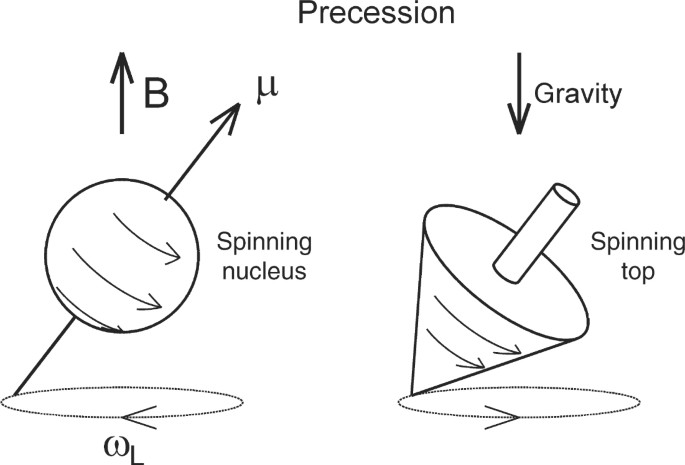
\includegraphics[width = 0.45 \textwidth]{figures/lamor.jpg}
    \caption{Left, model of Larmor precession of the nuclear spin about the direction of a steady applied magnetic field \textbf{B}. Right, analogous system a spinning top in a gravitational field.~\cite{Prasad2008}}
    \label{fig:lamor}
\end{figure}

  In the classical description of the resonance condition a rotating charge can be treated as a circulating current loop and as a result will have a magnetic dipole ($\mu$) described by $\mu = iA$, where `$i$' is the current and `$A$' is the cross-sectional area of the enclosed loop.~\cite{nmr65} However, as a proton is quantum object its magnetic moment is characterized by $\mu = \hbar \gamma \mathbf{I}$, where $\gamma$ is magnetogyric ratio and \textbf{I} is the magnetic quantum number given by nuclear spin.~\cite{nmr65}  When the a nucleon with magnetic moment $\mu$ is placed in a magnetic field the Hamiltonian for the system is given by

  \begin{gather}
    \mathscr{H} = -\mathbf{\mu}\cdot \mathbf{B} = -\hbar \gamma\mathbf{I}\cdot \mathbf{B} 
  \end{gather}
  with eigenvalues given by equation~\ref{eq:eigval}, ~\cite{nmr65}
  \begin{gather}
    E = \hbar \gamma m_z B_0 \label{eq:eigval}\\
    \Delta E = 2 \hbar \gamma m_z B_0 \label{eq:esplit}
  \end{gather}
  In the case of a proton $m_z = \pm 1/2$. This causes an energy split given by equation~\ref{eq:esplit} between the two levels as one state will align with the applied magnetic field while the other will be anti-aligned. Here m$_z$ are the projected values of \textbf{I} onto the z-axis defined by the magnetic field. 


  As this motion is akin to a harmonic oscillator we can set the energy difference equal to a characteristic, or in this case resonant frequency. The harmonic motion is the rotation or precession about the axis of the applied magnetic field. A toy model of this can be seen in figure~\ref{fig:lamor}. 

  \begin{gather}
    \Delta E_{proton} = \hbar \omega =  \hbar \gamma B_0 \nonumber \\
    \omega_0 = \gamma B_0 \rightarrow f_0 = \frac{\gamma B_0}{2 \pi}
  \end{gather}

  In properly address macroscopic samples we must define a net magnetization $\mathbf{M} = \sum_{i} \mu_i$. Now  we are able to look at a population of spins precessing about an applied magnetic field axis. However, the current model is only useful in a static equilibrium system, so in order to see the time evolution we can consider the system relaxing \textit{towards} equilibrium under the influence of an applied magentic field $\mathbf{B} = B_0 \hat{z}$ and solve the differential equation as shown by equations~\ref{eq:diff1}--\ref{eq:mzt1}.

\begin{gather}
    \mathbf{M}|_{\mathbf{B}} = M_0 \hat{z} \label{eq:diff1} \\
    \frac{dM_z}{dt} = \frac{M_0 - M_{z}}{T_1} \\
    M_z(t) = M_0 \left(1-2 e^\frac{-t}{T_1}\right) \label{eq:mzt1}
\end{gather}

  Here we took $M_z(t=0) = -M_0$, such that the initial magnetization vector pointed in the $-\hat{z}$-axis.This corresponds to complete anti-alignment with the applied field. Notice that we included a characteristic constant $T_1$, which is a characteristic constant that corresponds to the spin-lattice relaxation constant. This name comes from how the spins give the energy gained from the RF pulse to the surrounding lattice.~\cite{nmr65}

  The previous analysis fails to take into account the transverse magnetizations $M_x$ and $M_y$. This can be treated by solving the differential equation

  \begin{gather}
    \frac{dM_{i^*}}{dt} = \frac{M_0 - M_{i^*}}{T_2} \\
    \text{where } i = x , y
  \end{gather}


  Solving this system gives a simple exponential, with a characteristic time constant \tg that defines the spin-spin relaxation time constant (eq~\ref{eq:mzt2_wrong}). However, the signal due to the pulse is difficult to measure experimentally as there is some loss of the transverse magnetization due to stochastic fluctuations in the local nuclear fields. ~\cite{manual} As a result the spin echo is typically measured instead (equation~\ref{eq:mzt2}). 

  \begin{gather}
    M_{x,y}(t) = M_0  e^\frac{-t}{T_2}  \label{eq:mzt2_wrong}\\
    M_{x,y}(2\tau) = M_0  e^\frac{-2\tau}{T_2}  \label{eq:mzt2}
  \end{gather}

  The spin echo is related to how the spins dephase and rephase. Once the system is allowed to evolve the nuclear spins can precess in any direction as a result the measured signal is lost. If the spins are pulsed with a RF wave, they can be forced to realign themselves. This realignment and subsequent thermalization is the spin echo. In order to probe this various pulse sequences are used to coax the nuclear spins into behaving as desired.  


\section*{Experimental }

\subsection*{Equipment}

    \begin{figure}[h]
      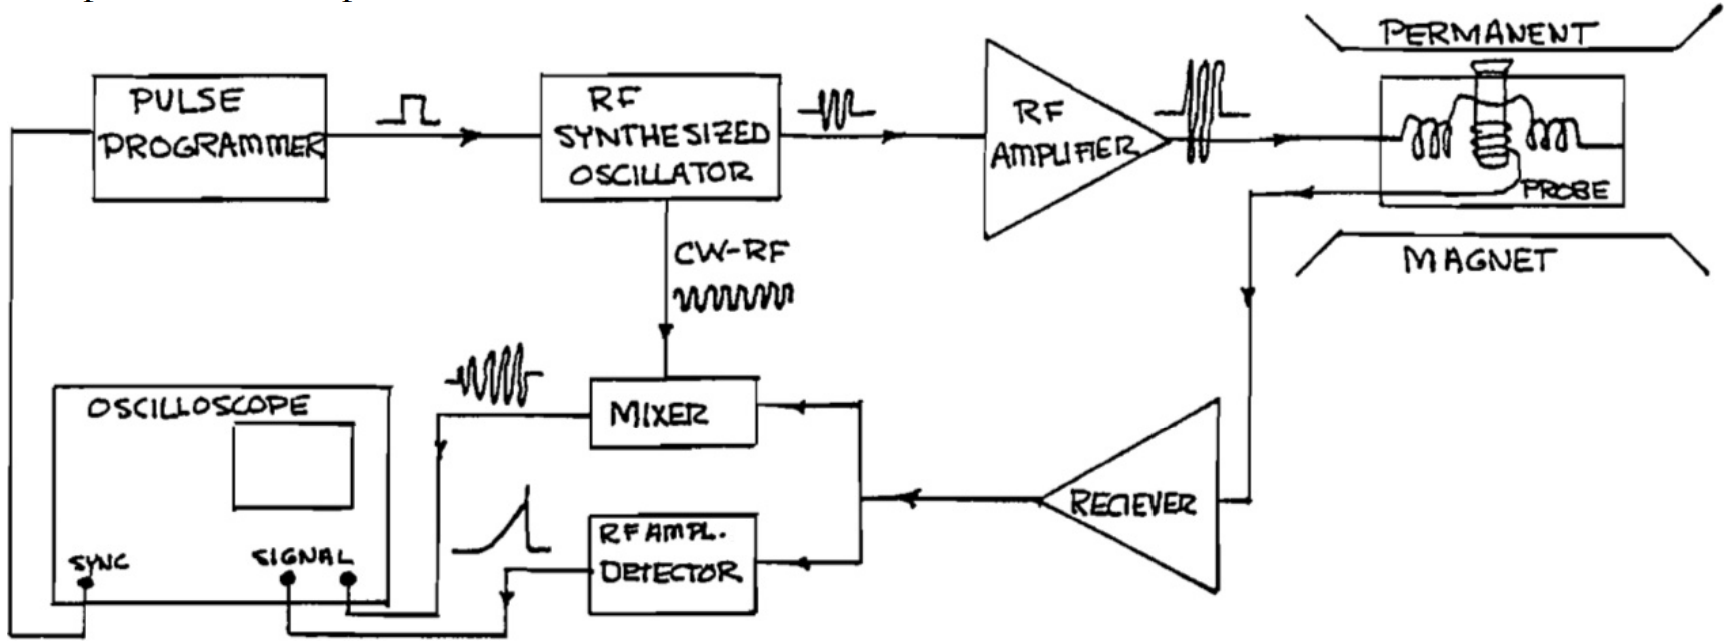
\includegraphics[width=0.4 \textwidth]{figures/block_diagram.png}
      \caption{Block diagram of experimental set up.\cite{manual}}
      \label{fig:block}
    \end{figure}


    For these experiments, a TeachSpin PS1-A system was used to produce/amplify the pulse sequences, and pickup/amplify the output signal. The signal was then processed/synced and displayed on a Tektronix TBS 1052B Digital Oscilloscope. A simplified block diagram of the system is shown in figure~\ref{fig:block}. The pulse sequence begins at the \textbf{pulse programer}. The exact number of pulses, their widths, and time characteristics are defined in this module. This sends two signals, the first goes to the \textbf{oscilloscope}, the second to the \textbf{RF synthesized oscillator}. This first signal is to let the oscilloscope know when a output signal is coming. The second signal tells the RF synthesized oscillator what pulse sequence to generate. From there the pulse sequence is sent to an \textbf{RF amplifier} and the \textbf{mixer}. The amplifier ensure that a strong enough signal sequence is transmitted to the transmitter Helmholtz coils in the sample chamber such that it influences the nuclear spins. The mixer combines the reference signal with the sample output signal. Before getting to the mixer the sample output signal goes to the \textbf{receiver}. The receiver also sends the output signal to a \textbf{RF amplifier detector}. The mixer and RF amplifier detector both send the signal to the oscilloscope. 
    
    The \textbf{pulse programer} outputs pulses that are about 4V with a rise time of 15ns. The length of these pulses can be controlled with the A-width or B-width knobs and ranges from 1-30$\mu$s. The two knobs exists because it is able to program the number of pulses. Its capable of producing 1 A-pulse and between 0-99 B-pulses for a maximum of 100 pulses. It also can set the delay time ($\tau$) between pulses. This is done using the dial switches between the pulse width knobs.  If there are more than one B-pulses then the delay between the B-pulses is 2$\tau$. The repetition time knobs in the center of the module decide how long to wait before starting the next pulse train. 
    
    \begin{figure}[h]
      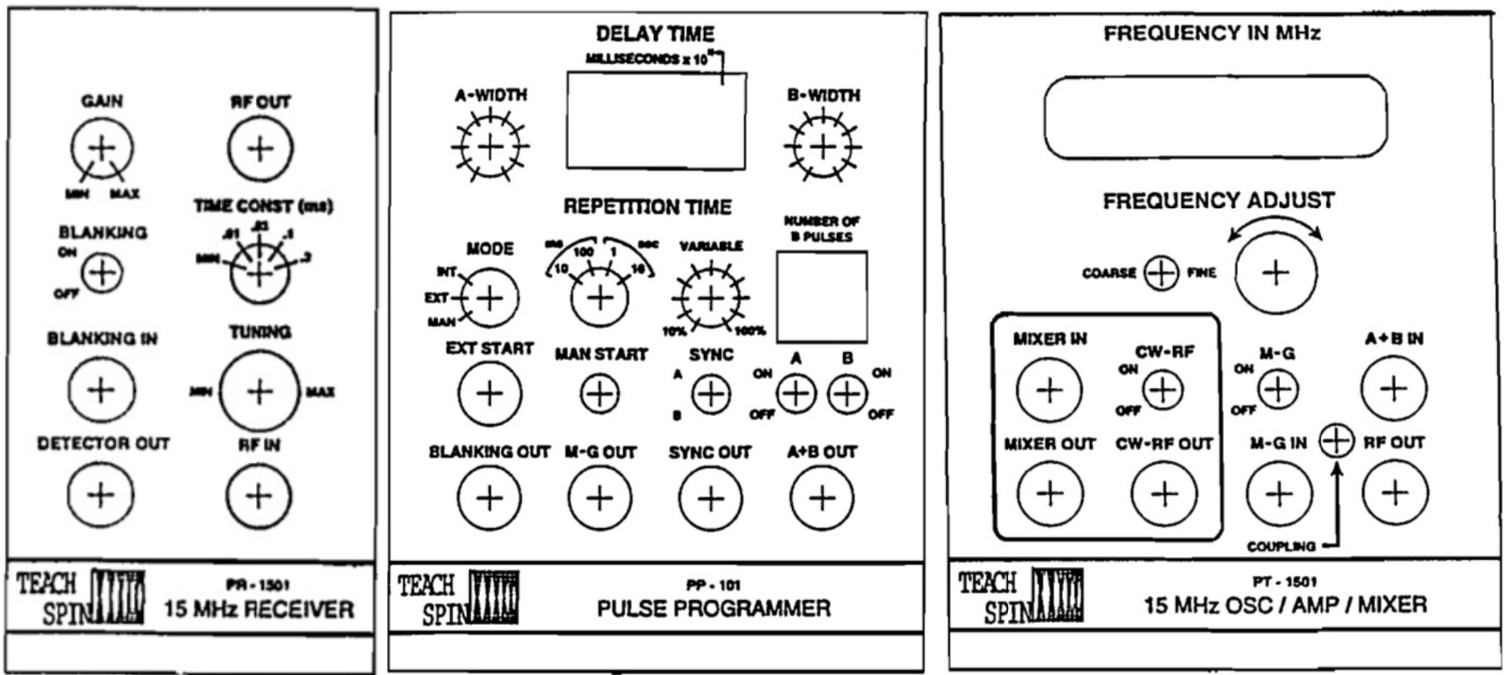
\includegraphics[width=0.48 \textwidth]{figures/threemods.jpg}
      \caption{Left to right: The spectrometer's receiver, pulse programer, and RF synthesized oscillator/amplifier/mixer modules.\cite{manual}}
      \label{fig:threemods}
    \end{figure}


    The \textbf{RF synthesized oscillator}, \textbf{RF amplifier}, and \textbf{mixer} are all part of one module. For the most part this module sends and receives signals. There are two tunable parameters in this module though. The first is the ability to adjust the transmitted frequency using the frequency adjust knob. The second is a switch that allows the user to turn on the MG corrections. 
    
    The \textbf{receiver} is the last module. It picks up the signal from the sample probe. The blanking switch tells the receiver to ignore the part of the output signal that comes from the excitation pulse. This is generally kept on. The gain knob controls the output to input signal ratio, this acts as a form of noise control. The time constant knob controls the RC time constant of the detector output. It also removes noise but can also distort the desired signal if its too high. The final knob is the tuning knob which tunes the receiver to the first stage of the amplifier.~\cite{manual}


    \begin{figure}[h]
      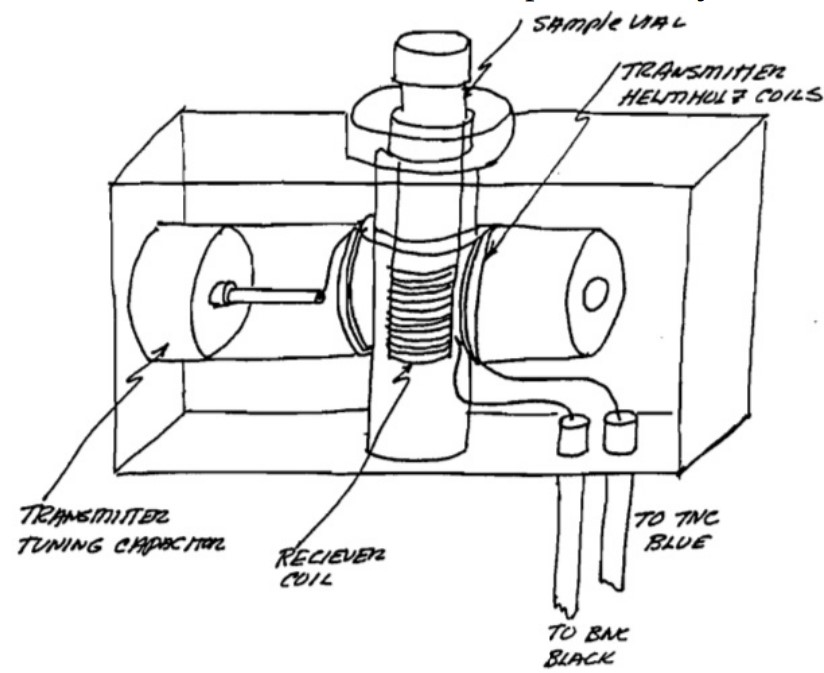
\includegraphics[width=0.4 \textwidth]{figures/probe.jpg}
      \caption{NMR Sample probe.\cite{manual}}
      \label{fig:probe}
    \end{figure}

    The sample probe is comprised of 5 major components (fig~\ref{fig:probe}). First there is the casing which houses the permanent ferromagnet. Secondly, there is a center region where the sample is held. The third component are the transmitter Helmholtz coils. These are made of two induction coils perpendicular to both the sample vial and the permanent magnet. The receiver coils are wrapped around the sample vial. The impedance of this induction coil changes with respect to the magnetization of the sample. When a component of the magnetization vector passes through the area inclosed by loop, it acts as a magnetic flux that increases or decreases the impedance. The final component are the sample placement dials on the outside of the housing. 

    The final component of the experimental set up is the oscilloscope. This instrument served as the screen where our data was shown. In order to ensure that the signal appeared in the same spot of the screen, the oscilloscope received a trigger signal from the pulse generator. Additionally to ensure that the data is easily readable its imporant to set the voltage (y-axis) to either 1 or 2 V using the yellow and/or blue vertical scale knobs. The horizontal scale knob controls how much time a single box on the oscilloscope grid is. 

\subsection*{Procedure}

\subsubsection*{Sample Preparation} 
    The two chemical species of interest were mineral oil, and CuSO$_{4} \boldsymbol{\cdot} $H$_2$O. The mineral oil was used as purchased from supplier. As CuSO$_{4}$ is a blue crystalline solid it was dissolved in deionized water prior to measurement.Seven sample concentrations of 0.005M, 0.01M, 0.05M, 0.1M, 0.2M 0.5M, \& 1M \cuso were prepared. 

    Chemical species were loaded into their own glass sample vials. Samples should be approximately cubical (~5mm tall) so that the magnetic field is experienced uniformly in the entire sample. Sample vials are caped with a rubber stop to ensure that concentrations are consistent and there is minimal evaporation or contamination. A rubber o-ring was used to adjust the sample depth inside of the probe. The optimal depth maximizes the signal amplitude and is roughly 1.5 inches from the bottom of the sample vial. The o-ring was placed at the same height for all sample. 


\subsubsection*{Single pulse FID}
    
    The procedure used in this section are used for the rest of the sections as well, as the goal of this section is to get a spectra that is in resonance. It should be assumed that for all measurements after this that this section is repeated.

    In order to maximize signal output on the oscilloscope, the spectrometer receiver must be tuned. First the signal to noise ratio must be reasonable. There are two parameters that control this. The gain knob on the receiver was set to 50\%. Additionally, the time constant knob was set to 0.1ms, because above this point the signal amplitude decreased. From there the spectrometer was tuned using the tuning knob is located on the receiver. This knob turns a capacitor inside the receiver and should be rotated in such a way that the signal amplitude is maximized. These parameters are relatively consistent between samples however some minor tuning may be necessary.

    On the pulse programer the mode was set to int. Additionally, the repetition time is set to be long enough for the magnetization vector to return to its equilibrium position. In the case of mineral oil we set the repetition time to 500 ms. At this point, the pulse sequence needs to be programed. Each sequence is unique but the programming of them is procedurally the same. In the case of the one pulse free induction decay (FID) pulse sequence we have a single $90^\circ$ A-pulse. However, other sequences may have multiple pulses. In those cases you turn on the B-pulses as well, select the number of B-pulses and choose the desired B-pulse-angle in a similar manner to the A-pulse. 

    To find the desired pulse angle the A- or B-width knob is rotated clockwise starting from the zero point. For a $90^\circ$ pulse the signal amplitude will be at a maximum. On our instrument that was about 20\% of the way on. It is recommended that while finding the desired pulse length the other pulse is turned off and the sync is set to the pulse of interest. For example, if tuning the B-pulse to $90^\circ$ the A-pulse should be switched off, the sync should be on B and the number of pulses should be 1. This is so that no other factors influence the peak amplitude. The same is true when tuning the A-pulse; B-pulse should be off and sync set to A. 

    
    \begin{figure}
        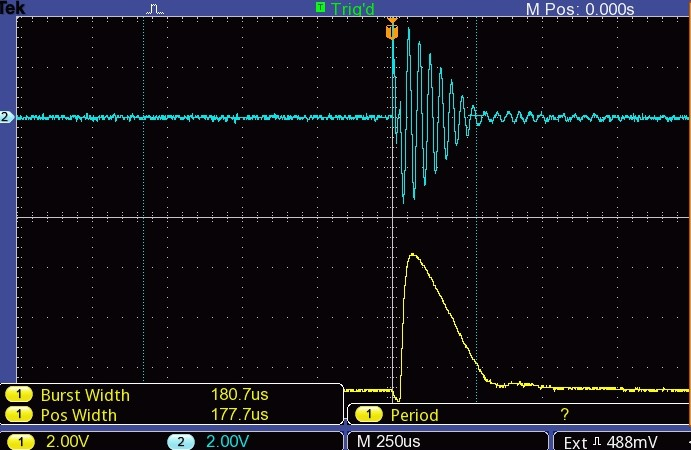
\includegraphics[width= 0.45\textwidth]{figures/noResonance.JPG}
        \caption{Single Pulse Free Induction Decay (FID) when out of resonance.}
        \label{fig:beats}
    \end{figure}

    \begin{figure}
      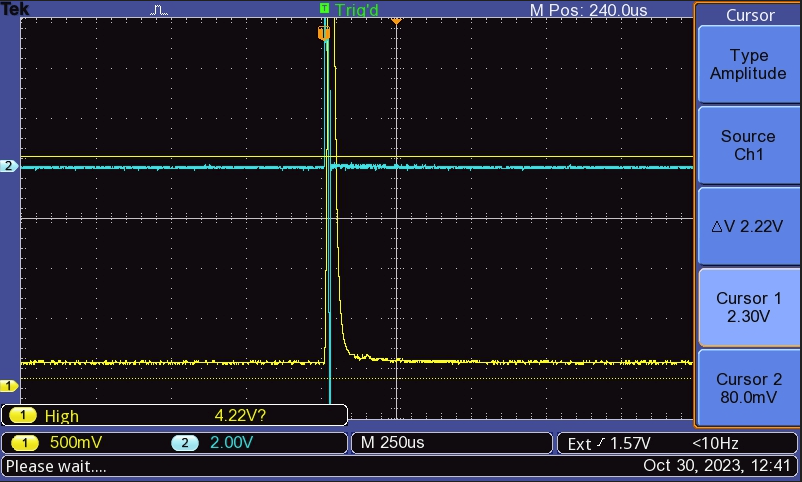
\includegraphics[width= 0.45\textwidth]{figures/FID-2.png}
      \caption{Single Pulse Free Induction Decay (FID) when out of resonance.}
      \label{fig:fid}
  \end{figure}

    As the magnet is $\sim 0.35$ Tesla, the resonant frequency will be around 15MHz. To find resonant frequency the frequency adjust knob is rotated until the mixer out spectra on the oscilloscope doesn't show any ``beats''. If the frequency is incorrect the displayed pulse will have multiple peaks within a single pulse, this is known as a beat (figure~\ref{fig:beats}). The resonance condition is when there is a single clean line that outlines a pulse or if it is perfectly flat (fig~\ref{fig:fid}). 

    Taking these parameters into account in order to acquire a single pulse FID of mineral oil the spectrometer must be set to output only the A-pulse, with a width of $\sim 20\%$, and a repetition time of 500m. From there a single clean pulse was found by tuning the frequency to 15.42707 MHz. A screenshot of the oscilloscope was taken. 

\subsubsection*{Magnetic Field Contours}

    In order to maximize signal amplitude the spatial dependence of the magnetic field was mapped so the sample can be placed in the section with the most uniform field. This was done by finding the resonant frequency at every point in a regular grid. Field uniformity is determined by a region with minimal change in the resonant frequency. Due to thermal effects the resonant frequency of the magnet drifts over time, thus  it is crucial to take these measurements rapidly. As the constant magnetic field $(B_0)$ was produced by a permanent ferromagnet, magnetic domain effects come into play. Some domains may be smaller than other and the most uniform field may not necessarily be in the center. However, it is also critical to avoid edge effects. 
    
    The direction of $B_0$ is parallel to the table top and will be called the z-axis. The sample holder allowed for freedom of movement in the x and y directions. Here the y-axis moved the sample up and down relative to table surface, while the x-direction moved the sample parallel to the surface but perpendicular to $B_0$. The values of the y-axis range from $0\ldots20~cm$ and begin at the bottom of the magnet and finish at the top. The x-axis places its zero point at the center of the magnet and ranges from $-10\ldots10~cm$. The field was mapped from $-1~cm \leq x \leq +1~cm$ with step sizes of $0.2~cm$ and from $9~cm \leq y \leq 11~cm$ with step sizes of $0.5~cm$. The resonance frequency values were mapped onto a contour plot and the section with the least change  in the resonant frequency was determined to have the most uniform magnetic field. 

\subsubsection*{Spin-Lattice Relaxation: T1 Sequence}


    A quick estimate of T$_1$ was acquired. First the spectrometer was set to resonance for a single pulse FID with a large repetition time. The repetition time was slowly lowered until the maximum amplitude of the FID decreased. The point just before the amplitude decrease is $\sim 4-5\times$T$_1$.

    For accurate measurement of T$_1$ a two pulse sequence of: $180^{\circ}- \tau \text{(variable)} - 90^{\circ}\text{ (FID)}$. An $180^{\circ}$ pulse is characterized by the amplitude of the pulse of interest being at a minimum, while a $90^{\circ}$ pulse is when the pulse amplitude is at a maximum as previously stated. So in this sequence the `A' pulse should be a minimum while the `B' pulse is maximized. However, if the sample is back in alignment with $B_0$ the signal received after the B-pulse will be unchanging. Thus by varying the delay time $(\tau )$ the amplitude of the B-pulse will vary until the saturation point is reached. By measuring the B-pulse amplitude over a range of delay times a fit can be made to equation~\ref{eq:mzt1}. \textbf{Note:} as the oscilloscope outputs the magnitude of the signal it will first appear as the signal is decreasing then increasing once it reaches zero see fig~\ref{fig:magnetization_t1}. Also for ease of measurement insure that pulse programer is synced to the B-pulse makes the measurement easier. 

    \begin{center}
        \begin{figure}[b]
            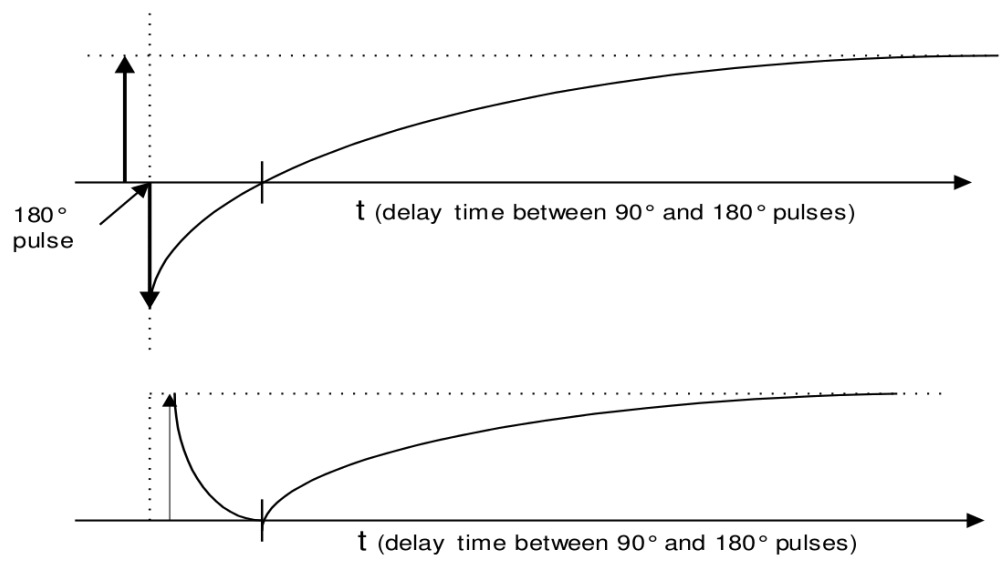
\includegraphics[width=0.4\textwidth]{figures/t1_pulse_magnetization.png}
            \caption{Top the z-component of the magnetization $(M_z)$vector over time. Bottom the amplitude of the magnetization.}
            \label{fig:magnetization_t1}
          \end{figure}
    \end{center}

\subsubsection*{Spin-Echo and Carl-Purcell methods}

    Both spin-echo and the Carl-Purcell method of measuring $T_2$ were only done on the mineral oil sample as the Meiboom-Gill pulse sequence is more accurate in nearly all cases.

    The spin-echo sequence is also a two pulse method however its sequence is: $90^{\circ}- \tau  - 180^{\circ}-\tau-\text{echo(at $2\tau$)}$. Similar to the $T_1$ measurement the signal amplitude decays as a function of the delay time. Thus the delay was varied by intervals of 10. The first two values were 1.5ms and 10ms and measurements ended at 90ms. The amplitudes were measured at varying delay times just like in the $T_1$ two-pulse method. A plot of delay time versus spin-echo amplitude was made and the $T_2$ was found by fitting equation~\ref{eq:mzt2}.

    The CP sequence is like the spin-echo method but with multiple B-pulses. Its sequence is: $90^{\circ}- \tau  - 180^{\circ}-2\tau- 180^{\circ}-2\tau- \dots$. Here the choice of delay time is critical as the spacing $2\tau$ should be short compared to the diffusion time of the spin through the magnetic field gradient. We used a delay time of 5 ms and 80 B-pulses for our measurements. The oscilloscope output was frozen and the spin-echo amplitude was measured at 10 points in intervals of $\sim$16 ms between peaks. Again the results were plotted and fitted to equation~\ref{eq:mzt2}.


    \begin{table}
    \begin{center}
    \begin{tabular}[t]{ |c|c|c| }
        \hline
        \multicolumn{3}{|c|}{Mineral Oil} \\ \hline 
        Molarity (mol/L) & Delay Time (ms) & Num. Pulses \\ \hline
        - & 4 & 60 \\ \hline 
    
        \multicolumn{3}{|c|}{CuSO$_{4} \boldsymbol{\cdot} $H$_2$O} \\ \hline
        Molarity (mol/L) & Delay Time (ms) & Num. Pulses \\ \hline
        0.005 M & 4 & 50 \\ \hline 
        0.01 M & 4 & 40  \\ \hline
        0.05 M & 1 & 50  \\ \hline 
        0.1 M & 0.8 & 50  \\ \hline
        0.2 M & 0.8 & 50  \\ \hline 
        0.5 M & 0.8 & 50  \\ \hline
        1.0 M & 0.1 & 20  \\ \hline 
    \end{tabular}
    \caption{The delay time and number of pulses used in the Meiboom-Gill pulse sequence for each mineral oil and \cuso. }
    \label{tab:delaytime}
    \end{center}
    \end{table}

\subsubsection*{Meiboom-Gill method}

    The MG method was used to find $T_2$ for the mineral oil and all the \cuso samples. This sequence is nearly identical to the CP sequence the only difference is that the $180^\circ$ pulses alternate in their direction; i.e. the sequence is $90^{\circ}- \tau  - 180^{\circ}-2\tau- ^{-}180^{\circ}-2\tau- 180^{\circ}\dots$. This is accomplished by turning on the MG switch on the pulse amplifier/mixer. The output signal was frozen on the oscilloscope monitor and 10--15 amplitudes were measured at regular time intervals. As the spin diffusion time is dependent on the chemical species and environment the optimal delay time and number of pulses changed between samples. Table~\ref{tab:delaytime} displays the values used in our lab. The results for each chemical species and concentration were plotted and fitted to equation~\ref{eq:mzt2}.


\section*{Results \lowercase{and} Discussion }

    The measured $T_1$ and $T_2$ values for both mineral oil and \cuso are summarized in table~\ref{tab:summery}. Additionally, detailed plots for all of the \cuso concentrations can be found in the Appendix. These sections will discuss the trends in the results with key examples.
  
\subsubsection*{Magnetic Field Contours}

  \begin{figure}[h]
    \resizebox{0.45\textwidth}{!}{%% Creator: Matplotlib, PGF backend
%%
%% To include the figure in your LaTeX document, write
%%   \input{<filename>.pgf}
%%
%% Make sure the required packages are loaded in your preamble
%%   \usepackage{pgf}
%%
%% Also ensure that all the required font packages are loaded; for instance,
%% the lmodern package is sometimes necessary when using math font.
%%   \usepackage{lmodern}
%%
%% Figures using additional raster images can only be included by \input if
%% they are in the same directory as the main LaTeX file. For loading figures
%% from other directories you can use the `import` package
%%   \usepackage{import}
%%
%% and then include the figures with
%%   \import{<path to file>}{<filename>.pgf}
%%
%% Matplotlib used the following preamble
%%   \usepackage{fontspec}
%%   \setmainfont{DejaVuSerif.ttf}[Path=\detokenize{/usr/share/matplotlib/mpl-data/fonts/ttf/}]
%%   \setsansfont{DejaVuSans.ttf}[Path=\detokenize{/usr/share/matplotlib/mpl-data/fonts/ttf/}]
%%   \setmonofont{DejaVuSansMono.ttf}[Path=\detokenize{/usr/share/matplotlib/mpl-data/fonts/ttf/}]
%%
\begingroup%
\makeatletter%
\begin{pgfpicture}%
\pgfpathrectangle{\pgfpointorigin}{\pgfqpoint{6.400000in}{4.800000in}}%
\pgfusepath{use as bounding box, clip}%
\begin{pgfscope}%
\pgfsetbuttcap%
\pgfsetmiterjoin%
\definecolor{currentfill}{rgb}{1.000000,1.000000,1.000000}%
\pgfsetfillcolor{currentfill}%
\pgfsetlinewidth{0.000000pt}%
\definecolor{currentstroke}{rgb}{1.000000,1.000000,1.000000}%
\pgfsetstrokecolor{currentstroke}%
\pgfsetdash{}{0pt}%
\pgfpathmoveto{\pgfqpoint{0.000000in}{0.000000in}}%
\pgfpathlineto{\pgfqpoint{6.400000in}{0.000000in}}%
\pgfpathlineto{\pgfqpoint{6.400000in}{4.800000in}}%
\pgfpathlineto{\pgfqpoint{0.000000in}{4.800000in}}%
\pgfpathlineto{\pgfqpoint{0.000000in}{0.000000in}}%
\pgfpathclose%
\pgfusepath{fill}%
\end{pgfscope}%
\begin{pgfscope}%
\pgfsetbuttcap%
\pgfsetmiterjoin%
\definecolor{currentfill}{rgb}{1.000000,1.000000,1.000000}%
\pgfsetfillcolor{currentfill}%
\pgfsetlinewidth{0.000000pt}%
\definecolor{currentstroke}{rgb}{0.000000,0.000000,0.000000}%
\pgfsetstrokecolor{currentstroke}%
\pgfsetstrokeopacity{0.000000}%
\pgfsetdash{}{0pt}%
\pgfpathmoveto{\pgfqpoint{1.485698in}{0.840429in}}%
\pgfpathlineto{\pgfqpoint{4.958681in}{0.840429in}}%
\pgfpathlineto{\pgfqpoint{4.958681in}{4.313411in}}%
\pgfpathlineto{\pgfqpoint{1.485698in}{4.313411in}}%
\pgfpathlineto{\pgfqpoint{1.485698in}{0.840429in}}%
\pgfpathclose%
\pgfusepath{fill}%
\end{pgfscope}%
\begin{pgfscope}%
\pgfpathrectangle{\pgfqpoint{1.485698in}{0.840429in}}{\pgfqpoint{3.472982in}{3.472982in}}%
\pgfusepath{clip}%
\pgfsetbuttcap%
\pgfsetroundjoin%
\definecolor{currentfill}{rgb}{0.020588,0.020588,0.028645}%
\pgfsetfillcolor{currentfill}%
\pgfsetlinewidth{0.000000pt}%
\definecolor{currentstroke}{rgb}{0.000000,0.000000,0.000000}%
\pgfsetstrokecolor{currentstroke}%
\pgfsetdash{}{0pt}%
\pgfpathmoveto{\pgfqpoint{4.958681in}{4.069795in}}%
\pgfpathlineto{\pgfqpoint{4.958681in}{4.313411in}}%
\pgfpathlineto{\pgfqpoint{4.717629in}{4.313411in}}%
\pgfpathlineto{\pgfqpoint{4.958681in}{4.069795in}}%
\pgfpathclose%
\pgfusepath{fill}%
\end{pgfscope}%
\begin{pgfscope}%
\pgfpathrectangle{\pgfqpoint{1.485698in}{0.840429in}}{\pgfqpoint{3.472982in}{3.472982in}}%
\pgfusepath{clip}%
\pgfsetbuttcap%
\pgfsetroundjoin%
\definecolor{currentfill}{rgb}{0.065196,0.065196,0.090708}%
\pgfsetfillcolor{currentfill}%
\pgfsetlinewidth{0.000000pt}%
\definecolor{currentstroke}{rgb}{0.000000,0.000000,0.000000}%
\pgfsetstrokecolor{currentstroke}%
\pgfsetdash{}{0pt}%
\pgfpathmoveto{\pgfqpoint{4.611382in}{4.004099in}}%
\pgfpathlineto{\pgfqpoint{4.958681in}{3.699174in}}%
\pgfpathlineto{\pgfqpoint{4.958681in}{4.069795in}}%
\pgfpathlineto{\pgfqpoint{4.717629in}{4.313411in}}%
\pgfpathlineto{\pgfqpoint{4.611382in}{4.313411in}}%
\pgfpathlineto{\pgfqpoint{4.428086in}{4.313411in}}%
\pgfpathlineto{\pgfqpoint{4.611382in}{4.004099in}}%
\pgfpathclose%
\pgfusepath{fill}%
\end{pgfscope}%
\begin{pgfscope}%
\pgfpathrectangle{\pgfqpoint{1.485698in}{0.840429in}}{\pgfqpoint{3.472982in}{3.472982in}}%
\pgfusepath{clip}%
\pgfsetbuttcap%
\pgfsetroundjoin%
\definecolor{currentfill}{rgb}{0.109804,0.109804,0.152771}%
\pgfsetfillcolor{currentfill}%
\pgfsetlinewidth{0.000000pt}%
\definecolor{currentstroke}{rgb}{0.000000,0.000000,0.000000}%
\pgfsetstrokecolor{currentstroke}%
\pgfsetdash{}{0pt}%
\pgfpathmoveto{\pgfqpoint{4.958681in}{2.478796in}}%
\pgfpathlineto{\pgfqpoint{4.958681in}{2.576920in}}%
\pgfpathlineto{\pgfqpoint{4.958681in}{3.445166in}}%
\pgfpathlineto{\pgfqpoint{4.958681in}{3.699174in}}%
\pgfpathlineto{\pgfqpoint{4.611382in}{4.004099in}}%
\pgfpathlineto{\pgfqpoint{4.428086in}{4.313411in}}%
\pgfpathlineto{\pgfqpoint{4.264084in}{4.313411in}}%
\pgfpathlineto{\pgfqpoint{4.212255in}{4.313411in}}%
\pgfpathlineto{\pgfqpoint{4.264084in}{4.137049in}}%
\pgfpathlineto{\pgfqpoint{4.611382in}{3.568620in}}%
\pgfpathlineto{\pgfqpoint{4.775987in}{3.445166in}}%
\pgfpathlineto{\pgfqpoint{4.835180in}{2.576920in}}%
\pgfpathlineto{\pgfqpoint{4.958681in}{2.478796in}}%
\pgfpathclose%
\pgfusepath{fill}%
\end{pgfscope}%
\begin{pgfscope}%
\pgfpathrectangle{\pgfqpoint{1.485698in}{0.840429in}}{\pgfqpoint{3.472982in}{3.472982in}}%
\pgfusepath{clip}%
\pgfsetbuttcap%
\pgfsetroundjoin%
\definecolor{currentfill}{rgb}{0.150980,0.150980,0.210060}%
\pgfsetfillcolor{currentfill}%
\pgfsetlinewidth{0.000000pt}%
\definecolor{currentstroke}{rgb}{0.000000,0.000000,0.000000}%
\pgfsetstrokecolor{currentstroke}%
\pgfsetdash{}{0pt}%
\pgfpathmoveto{\pgfqpoint{4.611382in}{2.561760in}}%
\pgfpathlineto{\pgfqpoint{4.958681in}{2.287901in}}%
\pgfpathlineto{\pgfqpoint{4.958681in}{2.478796in}}%
\pgfpathlineto{\pgfqpoint{4.835180in}{2.576920in}}%
\pgfpathlineto{\pgfqpoint{4.775987in}{3.445166in}}%
\pgfpathlineto{\pgfqpoint{4.611382in}{3.568620in}}%
\pgfpathlineto{\pgfqpoint{4.264084in}{4.137049in}}%
\pgfpathlineto{\pgfqpoint{4.212255in}{4.313411in}}%
\pgfpathlineto{\pgfqpoint{4.070058in}{4.313411in}}%
\pgfpathlineto{\pgfqpoint{4.264084in}{3.653183in}}%
\pgfpathlineto{\pgfqpoint{4.394321in}{3.445166in}}%
\pgfpathlineto{\pgfqpoint{4.588088in}{2.576920in}}%
\pgfpathlineto{\pgfqpoint{4.611382in}{2.561760in}}%
\pgfpathclose%
\pgfusepath{fill}%
\end{pgfscope}%
\begin{pgfscope}%
\pgfpathrectangle{\pgfqpoint{1.485698in}{0.840429in}}{\pgfqpoint{3.472982in}{3.472982in}}%
\pgfusepath{clip}%
\pgfsetbuttcap%
\pgfsetroundjoin%
\definecolor{currentfill}{rgb}{0.195588,0.195588,0.272123}%
\pgfsetfillcolor{currentfill}%
\pgfsetlinewidth{0.000000pt}%
\definecolor{currentstroke}{rgb}{0.000000,0.000000,0.000000}%
\pgfsetstrokecolor{currentstroke}%
\pgfsetdash{}{0pt}%
\pgfpathmoveto{\pgfqpoint{4.264084in}{2.565957in}}%
\pgfpathlineto{\pgfqpoint{4.611382in}{2.340564in}}%
\pgfpathlineto{\pgfqpoint{4.958681in}{2.097006in}}%
\pgfpathlineto{\pgfqpoint{4.958681in}{2.287901in}}%
\pgfpathlineto{\pgfqpoint{4.611382in}{2.561760in}}%
\pgfpathlineto{\pgfqpoint{4.588088in}{2.576920in}}%
\pgfpathlineto{\pgfqpoint{4.394321in}{3.445166in}}%
\pgfpathlineto{\pgfqpoint{4.264084in}{3.653183in}}%
\pgfpathlineto{\pgfqpoint{4.070058in}{4.313411in}}%
\pgfpathlineto{\pgfqpoint{3.927860in}{4.313411in}}%
\pgfpathlineto{\pgfqpoint{4.141862in}{3.445166in}}%
\pgfpathlineto{\pgfqpoint{4.251681in}{2.576920in}}%
\pgfpathlineto{\pgfqpoint{4.264084in}{2.565957in}}%
\pgfpathclose%
\pgfusepath{fill}%
\end{pgfscope}%
\begin{pgfscope}%
\pgfpathrectangle{\pgfqpoint{1.485698in}{0.840429in}}{\pgfqpoint{3.472982in}{3.472982in}}%
\pgfusepath{clip}%
\pgfsetbuttcap%
\pgfsetroundjoin%
\definecolor{currentfill}{rgb}{0.240196,0.240196,0.334186}%
\pgfsetfillcolor{currentfill}%
\pgfsetlinewidth{0.000000pt}%
\definecolor{currentstroke}{rgb}{0.000000,0.000000,0.000000}%
\pgfsetstrokecolor{currentstroke}%
\pgfsetdash{}{0pt}%
\pgfpathmoveto{\pgfqpoint{4.264084in}{2.331356in}}%
\pgfpathlineto{\pgfqpoint{4.611382in}{2.119368in}}%
\pgfpathlineto{\pgfqpoint{4.958681in}{1.906111in}}%
\pgfpathlineto{\pgfqpoint{4.958681in}{2.097006in}}%
\pgfpathlineto{\pgfqpoint{4.611382in}{2.340564in}}%
\pgfpathlineto{\pgfqpoint{4.264084in}{2.565957in}}%
\pgfpathlineto{\pgfqpoint{4.251681in}{2.576920in}}%
\pgfpathlineto{\pgfqpoint{4.141862in}{3.445166in}}%
\pgfpathlineto{\pgfqpoint{3.927860in}{4.313411in}}%
\pgfpathlineto{\pgfqpoint{3.916786in}{4.313411in}}%
\pgfpathlineto{\pgfqpoint{3.591469in}{4.313411in}}%
\pgfpathlineto{\pgfqpoint{3.916786in}{3.489690in}}%
\pgfpathlineto{\pgfqpoint{3.927472in}{3.445166in}}%
\pgfpathlineto{\pgfqpoint{3.986246in}{2.576920in}}%
\pgfpathlineto{\pgfqpoint{4.264084in}{2.331356in}}%
\pgfpathclose%
\pgfusepath{fill}%
\end{pgfscope}%
\begin{pgfscope}%
\pgfpathrectangle{\pgfqpoint{1.485698in}{0.840429in}}{\pgfqpoint{3.472982in}{3.472982in}}%
\pgfusepath{clip}%
\pgfsetbuttcap%
\pgfsetroundjoin%
\definecolor{currentfill}{rgb}{0.240196,0.240196,0.334186}%
\pgfsetfillcolor{currentfill}%
\pgfsetlinewidth{0.000000pt}%
\definecolor{currentstroke}{rgb}{0.000000,0.000000,0.000000}%
\pgfsetstrokecolor{currentstroke}%
\pgfsetdash{}{0pt}%
\pgfpathmoveto{\pgfqpoint{1.522432in}{4.313411in}}%
\pgfpathlineto{\pgfqpoint{1.485698in}{4.313411in}}%
\pgfpathlineto{\pgfqpoint{1.485698in}{4.304527in}}%
\pgfpathlineto{\pgfqpoint{1.522432in}{4.313411in}}%
\pgfpathclose%
\pgfusepath{fill}%
\end{pgfscope}%
\begin{pgfscope}%
\pgfpathrectangle{\pgfqpoint{1.485698in}{0.840429in}}{\pgfqpoint{3.472982in}{3.472982in}}%
\pgfusepath{clip}%
\pgfsetbuttcap%
\pgfsetroundjoin%
\definecolor{currentfill}{rgb}{0.284804,0.284804,0.396249}%
\pgfsetfillcolor{currentfill}%
\pgfsetlinewidth{0.000000pt}%
\definecolor{currentstroke}{rgb}{0.000000,0.000000,0.000000}%
\pgfsetstrokecolor{currentstroke}%
\pgfsetdash{}{0pt}%
\pgfpathmoveto{\pgfqpoint{4.958681in}{0.840429in}}%
\pgfpathlineto{\pgfqpoint{4.958681in}{1.657875in}}%
\pgfpathlineto{\pgfqpoint{4.771266in}{0.840429in}}%
\pgfpathlineto{\pgfqpoint{4.958681in}{0.840429in}}%
\pgfpathclose%
\pgfusepath{fill}%
\end{pgfscope}%
\begin{pgfscope}%
\pgfpathrectangle{\pgfqpoint{1.485698in}{0.840429in}}{\pgfqpoint{3.472982in}{3.472982in}}%
\pgfusepath{clip}%
\pgfsetbuttcap%
\pgfsetroundjoin%
\definecolor{currentfill}{rgb}{0.284804,0.284804,0.396249}%
\pgfsetfillcolor{currentfill}%
\pgfsetlinewidth{0.000000pt}%
\definecolor{currentstroke}{rgb}{0.000000,0.000000,0.000000}%
\pgfsetstrokecolor{currentstroke}%
\pgfsetdash{}{0pt}%
\pgfpathmoveto{\pgfqpoint{3.916786in}{2.370320in}}%
\pgfpathlineto{\pgfqpoint{4.264084in}{2.096754in}}%
\pgfpathlineto{\pgfqpoint{4.611382in}{1.898173in}}%
\pgfpathlineto{\pgfqpoint{4.958681in}{1.715216in}}%
\pgfpathlineto{\pgfqpoint{4.958681in}{1.906111in}}%
\pgfpathlineto{\pgfqpoint{4.611382in}{2.119368in}}%
\pgfpathlineto{\pgfqpoint{4.264084in}{2.331356in}}%
\pgfpathlineto{\pgfqpoint{3.986246in}{2.576920in}}%
\pgfpathlineto{\pgfqpoint{3.927472in}{3.445166in}}%
\pgfpathlineto{\pgfqpoint{3.916786in}{3.489690in}}%
\pgfpathlineto{\pgfqpoint{3.591469in}{4.313411in}}%
\pgfpathlineto{\pgfqpoint{3.569488in}{4.313411in}}%
\pgfpathlineto{\pgfqpoint{3.222190in}{4.313411in}}%
\pgfpathlineto{\pgfqpoint{3.101820in}{4.313411in}}%
\pgfpathlineto{\pgfqpoint{3.222190in}{4.118695in}}%
\pgfpathlineto{\pgfqpoint{3.569488in}{3.553697in}}%
\pgfpathlineto{\pgfqpoint{3.612401in}{3.445166in}}%
\pgfpathlineto{\pgfqpoint{3.822825in}{2.576920in}}%
\pgfpathlineto{\pgfqpoint{3.916786in}{2.370320in}}%
\pgfpathclose%
\pgfusepath{fill}%
\end{pgfscope}%
\begin{pgfscope}%
\pgfpathrectangle{\pgfqpoint{1.485698in}{0.840429in}}{\pgfqpoint{3.472982in}{3.472982in}}%
\pgfusepath{clip}%
\pgfsetbuttcap%
\pgfsetroundjoin%
\definecolor{currentfill}{rgb}{0.284804,0.284804,0.396249}%
\pgfsetfillcolor{currentfill}%
\pgfsetlinewidth{0.000000pt}%
\definecolor{currentstroke}{rgb}{0.000000,0.000000,0.000000}%
\pgfsetstrokecolor{currentstroke}%
\pgfsetdash{}{0pt}%
\pgfpathmoveto{\pgfqpoint{1.790419in}{4.313411in}}%
\pgfpathlineto{\pgfqpoint{1.522432in}{4.313411in}}%
\pgfpathlineto{\pgfqpoint{1.485698in}{4.304527in}}%
\pgfpathlineto{\pgfqpoint{1.485698in}{4.239712in}}%
\pgfpathlineto{\pgfqpoint{1.790419in}{4.313411in}}%
\pgfpathclose%
\pgfusepath{fill}%
\end{pgfscope}%
\begin{pgfscope}%
\pgfpathrectangle{\pgfqpoint{1.485698in}{0.840429in}}{\pgfqpoint{3.472982in}{3.472982in}}%
\pgfusepath{clip}%
\pgfsetbuttcap%
\pgfsetroundjoin%
\definecolor{currentfill}{rgb}{0.329412,0.333150,0.454412}%
\pgfsetfillcolor{currentfill}%
\pgfsetlinewidth{0.000000pt}%
\definecolor{currentstroke}{rgb}{0.000000,0.000000,0.000000}%
\pgfsetstrokecolor{currentstroke}%
\pgfsetdash{}{0pt}%
\pgfpathmoveto{\pgfqpoint{4.611382in}{0.840429in}}%
\pgfpathlineto{\pgfqpoint{4.771266in}{0.840429in}}%
\pgfpathlineto{\pgfqpoint{4.958681in}{1.657875in}}%
\pgfpathlineto{\pgfqpoint{4.958681in}{1.708675in}}%
\pgfpathlineto{\pgfqpoint{4.958681in}{1.715216in}}%
\pgfpathlineto{\pgfqpoint{4.611382in}{1.898173in}}%
\pgfpathlineto{\pgfqpoint{4.264084in}{2.096754in}}%
\pgfpathlineto{\pgfqpoint{3.916786in}{2.370320in}}%
\pgfpathlineto{\pgfqpoint{3.822825in}{2.576920in}}%
\pgfpathlineto{\pgfqpoint{3.612401in}{3.445166in}}%
\pgfpathlineto{\pgfqpoint{3.569488in}{3.553697in}}%
\pgfpathlineto{\pgfqpoint{3.222190in}{4.118695in}}%
\pgfpathlineto{\pgfqpoint{3.101820in}{4.313411in}}%
\pgfpathlineto{\pgfqpoint{2.874891in}{4.313411in}}%
\pgfpathlineto{\pgfqpoint{2.527593in}{4.313411in}}%
\pgfpathlineto{\pgfqpoint{2.180295in}{4.313411in}}%
\pgfpathlineto{\pgfqpoint{1.832997in}{4.313411in}}%
\pgfpathlineto{\pgfqpoint{1.790419in}{4.313411in}}%
\pgfpathlineto{\pgfqpoint{1.485698in}{4.239712in}}%
\pgfpathlineto{\pgfqpoint{1.485698in}{4.174896in}}%
\pgfpathlineto{\pgfqpoint{1.819156in}{3.445166in}}%
\pgfpathlineto{\pgfqpoint{1.832997in}{3.290122in}}%
\pgfpathlineto{\pgfqpoint{2.180295in}{3.274039in}}%
\pgfpathlineto{\pgfqpoint{2.527593in}{3.343494in}}%
\pgfpathlineto{\pgfqpoint{2.776227in}{3.445166in}}%
\pgfpathlineto{\pgfqpoint{2.874891in}{3.614745in}}%
\pgfpathlineto{\pgfqpoint{2.983422in}{3.445166in}}%
\pgfpathlineto{\pgfqpoint{3.222190in}{3.309502in}}%
\pgfpathlineto{\pgfqpoint{3.569488in}{3.040179in}}%
\pgfpathlineto{\pgfqpoint{3.695562in}{2.576920in}}%
\pgfpathlineto{\pgfqpoint{3.916786in}{2.090494in}}%
\pgfpathlineto{\pgfqpoint{4.264084in}{1.862153in}}%
\pgfpathlineto{\pgfqpoint{4.548977in}{1.708675in}}%
\pgfpathlineto{\pgfqpoint{4.474714in}{0.840429in}}%
\pgfpathlineto{\pgfqpoint{4.611382in}{0.840429in}}%
\pgfpathclose%
\pgfusepath{fill}%
\end{pgfscope}%
\begin{pgfscope}%
\pgfpathrectangle{\pgfqpoint{1.485698in}{0.840429in}}{\pgfqpoint{3.472982in}{3.472982in}}%
\pgfusepath{clip}%
\pgfsetbuttcap%
\pgfsetroundjoin%
\definecolor{currentfill}{rgb}{0.370588,0.389767,0.495588}%
\pgfsetfillcolor{currentfill}%
\pgfsetlinewidth{0.000000pt}%
\definecolor{currentstroke}{rgb}{0.000000,0.000000,0.000000}%
\pgfsetstrokecolor{currentstroke}%
\pgfsetdash{}{0pt}%
\pgfpathmoveto{\pgfqpoint{4.264084in}{0.840429in}}%
\pgfpathlineto{\pgfqpoint{4.474714in}{0.840429in}}%
\pgfpathlineto{\pgfqpoint{4.548977in}{1.708675in}}%
\pgfpathlineto{\pgfqpoint{4.264084in}{1.862153in}}%
\pgfpathlineto{\pgfqpoint{3.916786in}{2.090494in}}%
\pgfpathlineto{\pgfqpoint{3.695562in}{2.576920in}}%
\pgfpathlineto{\pgfqpoint{3.569488in}{3.040179in}}%
\pgfpathlineto{\pgfqpoint{3.222190in}{3.309502in}}%
\pgfpathlineto{\pgfqpoint{2.983422in}{3.445166in}}%
\pgfpathlineto{\pgfqpoint{2.874891in}{3.614745in}}%
\pgfpathlineto{\pgfqpoint{2.776227in}{3.445166in}}%
\pgfpathlineto{\pgfqpoint{2.527593in}{3.343494in}}%
\pgfpathlineto{\pgfqpoint{2.180295in}{3.274039in}}%
\pgfpathlineto{\pgfqpoint{1.832997in}{3.290122in}}%
\pgfpathlineto{\pgfqpoint{1.819156in}{3.445166in}}%
\pgfpathlineto{\pgfqpoint{1.485698in}{4.174896in}}%
\pgfpathlineto{\pgfqpoint{1.485698in}{4.110080in}}%
\pgfpathlineto{\pgfqpoint{1.789538in}{3.445166in}}%
\pgfpathlineto{\pgfqpoint{1.832997in}{2.958328in}}%
\pgfpathlineto{\pgfqpoint{2.180295in}{2.984923in}}%
\pgfpathlineto{\pgfqpoint{2.527593in}{3.084473in}}%
\pgfpathlineto{\pgfqpoint{2.874891in}{3.133930in}}%
\pgfpathlineto{\pgfqpoint{3.222190in}{2.913612in}}%
\pgfpathlineto{\pgfqpoint{3.565713in}{2.576920in}}%
\pgfpathlineto{\pgfqpoint{3.569488in}{2.573863in}}%
\pgfpathlineto{\pgfqpoint{3.916786in}{1.810668in}}%
\pgfpathlineto{\pgfqpoint{4.095005in}{1.708675in}}%
\pgfpathlineto{\pgfqpoint{4.218346in}{0.840429in}}%
\pgfpathlineto{\pgfqpoint{4.264084in}{0.840429in}}%
\pgfpathclose%
\pgfusepath{fill}%
\end{pgfscope}%
\begin{pgfscope}%
\pgfpathrectangle{\pgfqpoint{1.485698in}{0.840429in}}{\pgfqpoint{3.472982in}{3.472982in}}%
\pgfusepath{clip}%
\pgfsetbuttcap%
\pgfsetroundjoin%
\definecolor{currentfill}{rgb}{0.415196,0.451103,0.540196}%
\pgfsetfillcolor{currentfill}%
\pgfsetlinewidth{0.000000pt}%
\definecolor{currentstroke}{rgb}{0.000000,0.000000,0.000000}%
\pgfsetstrokecolor{currentstroke}%
\pgfsetdash{}{0pt}%
\pgfpathmoveto{\pgfqpoint{1.521626in}{1.708675in}}%
\pgfpathlineto{\pgfqpoint{1.535314in}{2.576920in}}%
\pgfpathlineto{\pgfqpoint{1.485698in}{2.579251in}}%
\pgfpathlineto{\pgfqpoint{1.485698in}{2.576920in}}%
\pgfpathlineto{\pgfqpoint{1.485698in}{1.708675in}}%
\pgfpathlineto{\pgfqpoint{1.485698in}{1.689890in}}%
\pgfpathlineto{\pgfqpoint{1.521626in}{1.708675in}}%
\pgfpathclose%
\pgfusepath{fill}%
\end{pgfscope}%
\begin{pgfscope}%
\pgfpathrectangle{\pgfqpoint{1.485698in}{0.840429in}}{\pgfqpoint{3.472982in}{3.472982in}}%
\pgfusepath{clip}%
\pgfsetbuttcap%
\pgfsetroundjoin%
\definecolor{currentfill}{rgb}{0.415196,0.451103,0.540196}%
\pgfsetfillcolor{currentfill}%
\pgfsetlinewidth{0.000000pt}%
\definecolor{currentstroke}{rgb}{0.000000,0.000000,0.000000}%
\pgfsetstrokecolor{currentstroke}%
\pgfsetdash{}{0pt}%
\pgfpathmoveto{\pgfqpoint{3.916786in}{1.057490in}}%
\pgfpathlineto{\pgfqpoint{3.969501in}{0.840429in}}%
\pgfpathlineto{\pgfqpoint{4.218346in}{0.840429in}}%
\pgfpathlineto{\pgfqpoint{4.095005in}{1.708675in}}%
\pgfpathlineto{\pgfqpoint{3.916786in}{1.810668in}}%
\pgfpathlineto{\pgfqpoint{3.569488in}{2.573863in}}%
\pgfpathlineto{\pgfqpoint{3.565713in}{2.576920in}}%
\pgfpathlineto{\pgfqpoint{3.222190in}{2.913612in}}%
\pgfpathlineto{\pgfqpoint{2.874891in}{3.133930in}}%
\pgfpathlineto{\pgfqpoint{2.527593in}{3.084473in}}%
\pgfpathlineto{\pgfqpoint{2.180295in}{2.984923in}}%
\pgfpathlineto{\pgfqpoint{1.832997in}{2.958328in}}%
\pgfpathlineto{\pgfqpoint{1.789538in}{3.445166in}}%
\pgfpathlineto{\pgfqpoint{1.485698in}{4.110080in}}%
\pgfpathlineto{\pgfqpoint{1.485698in}{4.045265in}}%
\pgfpathlineto{\pgfqpoint{1.759920in}{3.445166in}}%
\pgfpathlineto{\pgfqpoint{1.832997in}{2.626534in}}%
\pgfpathlineto{\pgfqpoint{2.180295in}{2.695808in}}%
\pgfpathlineto{\pgfqpoint{2.527593in}{2.825451in}}%
\pgfpathlineto{\pgfqpoint{2.874891in}{2.765270in}}%
\pgfpathlineto{\pgfqpoint{3.143556in}{2.576920in}}%
\pgfpathlineto{\pgfqpoint{3.222190in}{2.524564in}}%
\pgfpathlineto{\pgfqpoint{3.569488in}{2.246742in}}%
\pgfpathlineto{\pgfqpoint{3.819998in}{1.708675in}}%
\pgfpathlineto{\pgfqpoint{3.916786in}{1.057490in}}%
\pgfpathclose%
\pgfusepath{fill}%
\end{pgfscope}%
\begin{pgfscope}%
\pgfpathrectangle{\pgfqpoint{1.485698in}{0.840429in}}{\pgfqpoint{3.472982in}{3.472982in}}%
\pgfusepath{clip}%
\pgfsetbuttcap%
\pgfsetroundjoin%
\definecolor{currentfill}{rgb}{0.459804,0.512439,0.584804}%
\pgfsetfillcolor{currentfill}%
\pgfsetlinewidth{0.000000pt}%
\definecolor{currentstroke}{rgb}{0.000000,0.000000,0.000000}%
\pgfsetstrokecolor{currentstroke}%
\pgfsetdash{}{0pt}%
\pgfpathmoveto{\pgfqpoint{1.832997in}{1.703337in}}%
\pgfpathlineto{\pgfqpoint{1.843850in}{1.708675in}}%
\pgfpathlineto{\pgfqpoint{2.180295in}{2.226282in}}%
\pgfpathlineto{\pgfqpoint{2.527593in}{2.560418in}}%
\pgfpathlineto{\pgfqpoint{2.874891in}{2.269905in}}%
\pgfpathlineto{\pgfqpoint{3.222190in}{2.174429in}}%
\pgfpathlineto{\pgfqpoint{3.569488in}{1.919622in}}%
\pgfpathlineto{\pgfqpoint{3.667699in}{1.708675in}}%
\pgfpathlineto{\pgfqpoint{3.703518in}{0.840429in}}%
\pgfpathlineto{\pgfqpoint{3.916786in}{0.840429in}}%
\pgfpathlineto{\pgfqpoint{3.969501in}{0.840429in}}%
\pgfpathlineto{\pgfqpoint{3.916786in}{1.057490in}}%
\pgfpathlineto{\pgfqpoint{3.819998in}{1.708675in}}%
\pgfpathlineto{\pgfqpoint{3.569488in}{2.246742in}}%
\pgfpathlineto{\pgfqpoint{3.222190in}{2.524564in}}%
\pgfpathlineto{\pgfqpoint{3.143556in}{2.576920in}}%
\pgfpathlineto{\pgfqpoint{2.874891in}{2.765270in}}%
\pgfpathlineto{\pgfqpoint{2.527593in}{2.825451in}}%
\pgfpathlineto{\pgfqpoint{2.180295in}{2.695808in}}%
\pgfpathlineto{\pgfqpoint{1.832997in}{2.626534in}}%
\pgfpathlineto{\pgfqpoint{1.759920in}{3.445166in}}%
\pgfpathlineto{\pgfqpoint{1.485698in}{4.045265in}}%
\pgfpathlineto{\pgfqpoint{1.485698in}{3.980449in}}%
\pgfpathlineto{\pgfqpoint{1.730302in}{3.445166in}}%
\pgfpathlineto{\pgfqpoint{1.485698in}{2.672777in}}%
\pgfpathlineto{\pgfqpoint{1.485698in}{2.579251in}}%
\pgfpathlineto{\pgfqpoint{1.535314in}{2.576920in}}%
\pgfpathlineto{\pgfqpoint{1.521626in}{1.708675in}}%
\pgfpathlineto{\pgfqpoint{1.485698in}{1.689890in}}%
\pgfpathlineto{\pgfqpoint{1.485698in}{1.522398in}}%
\pgfpathlineto{\pgfqpoint{1.832997in}{1.703337in}}%
\pgfpathclose%
\pgfusepath{fill}%
\end{pgfscope}%
\begin{pgfscope}%
\pgfpathrectangle{\pgfqpoint{1.485698in}{0.840429in}}{\pgfqpoint{3.472982in}{3.472982in}}%
\pgfusepath{clip}%
\pgfsetbuttcap%
\pgfsetroundjoin%
\definecolor{currentfill}{rgb}{0.504412,0.573774,0.629412}%
\pgfsetfillcolor{currentfill}%
\pgfsetlinewidth{0.000000pt}%
\definecolor{currentstroke}{rgb}{0.000000,0.000000,0.000000}%
\pgfsetstrokecolor{currentstroke}%
\pgfsetdash{}{0pt}%
\pgfpathmoveto{\pgfqpoint{1.832997in}{1.512964in}}%
\pgfpathlineto{\pgfqpoint{2.180295in}{1.677020in}}%
\pgfpathlineto{\pgfqpoint{2.217505in}{1.708675in}}%
\pgfpathlineto{\pgfqpoint{2.527593in}{2.152952in}}%
\pgfpathlineto{\pgfqpoint{2.844141in}{1.708675in}}%
\pgfpathlineto{\pgfqpoint{2.874891in}{1.667213in}}%
\pgfpathlineto{\pgfqpoint{2.959236in}{1.708675in}}%
\pgfpathlineto{\pgfqpoint{3.222190in}{1.824295in}}%
\pgfpathlineto{\pgfqpoint{3.389524in}{1.708675in}}%
\pgfpathlineto{\pgfqpoint{3.520135in}{0.840429in}}%
\pgfpathlineto{\pgfqpoint{3.569488in}{0.840429in}}%
\pgfpathlineto{\pgfqpoint{3.703518in}{0.840429in}}%
\pgfpathlineto{\pgfqpoint{3.667699in}{1.708675in}}%
\pgfpathlineto{\pgfqpoint{3.569488in}{1.919622in}}%
\pgfpathlineto{\pgfqpoint{3.222190in}{2.174429in}}%
\pgfpathlineto{\pgfqpoint{2.874891in}{2.269905in}}%
\pgfpathlineto{\pgfqpoint{2.527593in}{2.560418in}}%
\pgfpathlineto{\pgfqpoint{2.180295in}{2.226282in}}%
\pgfpathlineto{\pgfqpoint{1.843850in}{1.708675in}}%
\pgfpathlineto{\pgfqpoint{1.832997in}{1.703337in}}%
\pgfpathlineto{\pgfqpoint{1.485698in}{1.522398in}}%
\pgfpathlineto{\pgfqpoint{1.485698in}{1.354906in}}%
\pgfpathlineto{\pgfqpoint{1.832997in}{1.512964in}}%
\pgfpathclose%
\pgfusepath{fill}%
\end{pgfscope}%
\begin{pgfscope}%
\pgfpathrectangle{\pgfqpoint{1.485698in}{0.840429in}}{\pgfqpoint{3.472982in}{3.472982in}}%
\pgfusepath{clip}%
\pgfsetbuttcap%
\pgfsetroundjoin%
\definecolor{currentfill}{rgb}{0.504412,0.573774,0.629412}%
\pgfsetfillcolor{currentfill}%
\pgfsetlinewidth{0.000000pt}%
\definecolor{currentstroke}{rgb}{0.000000,0.000000,0.000000}%
\pgfsetstrokecolor{currentstroke}%
\pgfsetdash{}{0pt}%
\pgfpathmoveto{\pgfqpoint{2.527593in}{0.840429in}}%
\pgfpathlineto{\pgfqpoint{2.616703in}{0.840429in}}%
\pgfpathlineto{\pgfqpoint{2.527593in}{1.188322in}}%
\pgfpathlineto{\pgfqpoint{2.467126in}{0.840429in}}%
\pgfpathlineto{\pgfqpoint{2.527593in}{0.840429in}}%
\pgfpathclose%
\pgfusepath{fill}%
\end{pgfscope}%
\begin{pgfscope}%
\pgfpathrectangle{\pgfqpoint{1.485698in}{0.840429in}}{\pgfqpoint{3.472982in}{3.472982in}}%
\pgfusepath{clip}%
\pgfsetbuttcap%
\pgfsetroundjoin%
\definecolor{currentfill}{rgb}{0.504412,0.573774,0.629412}%
\pgfsetfillcolor{currentfill}%
\pgfsetlinewidth{0.000000pt}%
\definecolor{currentstroke}{rgb}{0.000000,0.000000,0.000000}%
\pgfsetstrokecolor{currentstroke}%
\pgfsetdash{}{0pt}%
\pgfpathmoveto{\pgfqpoint{1.730302in}{3.445166in}}%
\pgfpathlineto{\pgfqpoint{1.485698in}{3.980449in}}%
\pgfpathlineto{\pgfqpoint{1.485698in}{3.915634in}}%
\pgfpathlineto{\pgfqpoint{1.700684in}{3.445166in}}%
\pgfpathlineto{\pgfqpoint{1.485698in}{2.766303in}}%
\pgfpathlineto{\pgfqpoint{1.485698in}{2.672777in}}%
\pgfpathlineto{\pgfqpoint{1.730302in}{3.445166in}}%
\pgfpathclose%
\pgfusepath{fill}%
\end{pgfscope}%
\begin{pgfscope}%
\pgfpathrectangle{\pgfqpoint{1.485698in}{0.840429in}}{\pgfqpoint{3.472982in}{3.472982in}}%
\pgfusepath{clip}%
\pgfsetbuttcap%
\pgfsetroundjoin%
\definecolor{currentfill}{rgb}{0.549020,0.635110,0.674020}%
\pgfsetfillcolor{currentfill}%
\pgfsetlinewidth{0.000000pt}%
\definecolor{currentstroke}{rgb}{0.000000,0.000000,0.000000}%
\pgfsetstrokecolor{currentstroke}%
\pgfsetdash{}{0pt}%
\pgfpathmoveto{\pgfqpoint{1.832997in}{1.322590in}}%
\pgfpathlineto{\pgfqpoint{2.180295in}{1.435087in}}%
\pgfpathlineto{\pgfqpoint{2.384178in}{0.840429in}}%
\pgfpathlineto{\pgfqpoint{2.467126in}{0.840429in}}%
\pgfpathlineto{\pgfqpoint{2.527593in}{1.188322in}}%
\pgfpathlineto{\pgfqpoint{2.616703in}{0.840429in}}%
\pgfpathlineto{\pgfqpoint{2.738942in}{0.840429in}}%
\pgfpathlineto{\pgfqpoint{2.874891in}{1.275771in}}%
\pgfpathlineto{\pgfqpoint{3.222190in}{1.494600in}}%
\pgfpathlineto{\pgfqpoint{3.422343in}{0.840429in}}%
\pgfpathlineto{\pgfqpoint{3.520135in}{0.840429in}}%
\pgfpathlineto{\pgfqpoint{3.389524in}{1.708675in}}%
\pgfpathlineto{\pgfqpoint{3.222190in}{1.824295in}}%
\pgfpathlineto{\pgfqpoint{2.959236in}{1.708675in}}%
\pgfpathlineto{\pgfqpoint{2.874891in}{1.667213in}}%
\pgfpathlineto{\pgfqpoint{2.844141in}{1.708675in}}%
\pgfpathlineto{\pgfqpoint{2.527593in}{2.152952in}}%
\pgfpathlineto{\pgfqpoint{2.217505in}{1.708675in}}%
\pgfpathlineto{\pgfqpoint{2.180295in}{1.677020in}}%
\pgfpathlineto{\pgfqpoint{1.832997in}{1.512964in}}%
\pgfpathlineto{\pgfqpoint{1.485698in}{1.354906in}}%
\pgfpathlineto{\pgfqpoint{1.485698in}{1.187414in}}%
\pgfpathlineto{\pgfqpoint{1.832997in}{1.322590in}}%
\pgfpathclose%
\pgfpathmoveto{\pgfqpoint{2.501900in}{1.708675in}}%
\pgfpathlineto{\pgfqpoint{2.527593in}{1.745487in}}%
\pgfpathlineto{\pgfqpoint{2.553822in}{1.708675in}}%
\pgfpathlineto{\pgfqpoint{2.527593in}{1.665560in}}%
\pgfpathlineto{\pgfqpoint{2.501900in}{1.708675in}}%
\pgfpathclose%
\pgfusepath{fill}%
\end{pgfscope}%
\begin{pgfscope}%
\pgfpathrectangle{\pgfqpoint{1.485698in}{0.840429in}}{\pgfqpoint{3.472982in}{3.472982in}}%
\pgfusepath{clip}%
\pgfsetbuttcap%
\pgfsetroundjoin%
\definecolor{currentfill}{rgb}{0.549020,0.635110,0.674020}%
\pgfsetfillcolor{currentfill}%
\pgfsetlinewidth{0.000000pt}%
\definecolor{currentstroke}{rgb}{0.000000,0.000000,0.000000}%
\pgfsetstrokecolor{currentstroke}%
\pgfsetdash{}{0pt}%
\pgfpathmoveto{\pgfqpoint{1.700684in}{3.445166in}}%
\pgfpathlineto{\pgfqpoint{1.485698in}{3.915634in}}%
\pgfpathlineto{\pgfqpoint{1.485698in}{3.850818in}}%
\pgfpathlineto{\pgfqpoint{1.671066in}{3.445166in}}%
\pgfpathlineto{\pgfqpoint{1.485698in}{2.859829in}}%
\pgfpathlineto{\pgfqpoint{1.485698in}{2.766303in}}%
\pgfpathlineto{\pgfqpoint{1.700684in}{3.445166in}}%
\pgfpathclose%
\pgfusepath{fill}%
\end{pgfscope}%
\begin{pgfscope}%
\pgfpathrectangle{\pgfqpoint{1.485698in}{0.840429in}}{\pgfqpoint{3.472982in}{3.472982in}}%
\pgfusepath{clip}%
\pgfsetbuttcap%
\pgfsetroundjoin%
\definecolor{currentfill}{rgb}{0.590196,0.691728,0.715196}%
\pgfsetfillcolor{currentfill}%
\pgfsetlinewidth{0.000000pt}%
\definecolor{currentstroke}{rgb}{0.000000,0.000000,0.000000}%
\pgfsetstrokecolor{currentstroke}%
\pgfsetdash{}{0pt}%
\pgfpathmoveto{\pgfqpoint{1.832997in}{1.132217in}}%
\pgfpathlineto{\pgfqpoint{2.180295in}{1.193154in}}%
\pgfpathlineto{\pgfqpoint{2.301229in}{0.840429in}}%
\pgfpathlineto{\pgfqpoint{2.384178in}{0.840429in}}%
\pgfpathlineto{\pgfqpoint{2.180295in}{1.435087in}}%
\pgfpathlineto{\pgfqpoint{1.832997in}{1.322590in}}%
\pgfpathlineto{\pgfqpoint{1.485698in}{1.187414in}}%
\pgfpathlineto{\pgfqpoint{1.485698in}{1.019922in}}%
\pgfpathlineto{\pgfqpoint{1.832997in}{1.132217in}}%
\pgfpathclose%
\pgfusepath{fill}%
\end{pgfscope}%
\begin{pgfscope}%
\pgfpathrectangle{\pgfqpoint{1.485698in}{0.840429in}}{\pgfqpoint{3.472982in}{3.472982in}}%
\pgfusepath{clip}%
\pgfsetbuttcap%
\pgfsetroundjoin%
\definecolor{currentfill}{rgb}{0.590196,0.691728,0.715196}%
\pgfsetfillcolor{currentfill}%
\pgfsetlinewidth{0.000000pt}%
\definecolor{currentstroke}{rgb}{0.000000,0.000000,0.000000}%
\pgfsetstrokecolor{currentstroke}%
\pgfsetdash{}{0pt}%
\pgfpathmoveto{\pgfqpoint{2.527593in}{1.665560in}}%
\pgfpathlineto{\pgfqpoint{2.553822in}{1.708675in}}%
\pgfpathlineto{\pgfqpoint{2.527593in}{1.745487in}}%
\pgfpathlineto{\pgfqpoint{2.501900in}{1.708675in}}%
\pgfpathlineto{\pgfqpoint{2.527593in}{1.665560in}}%
\pgfpathclose%
\pgfusepath{fill}%
\end{pgfscope}%
\begin{pgfscope}%
\pgfpathrectangle{\pgfqpoint{1.485698in}{0.840429in}}{\pgfqpoint{3.472982in}{3.472982in}}%
\pgfusepath{clip}%
\pgfsetbuttcap%
\pgfsetroundjoin%
\definecolor{currentfill}{rgb}{0.590196,0.691728,0.715196}%
\pgfsetfillcolor{currentfill}%
\pgfsetlinewidth{0.000000pt}%
\definecolor{currentstroke}{rgb}{0.000000,0.000000,0.000000}%
\pgfsetstrokecolor{currentstroke}%
\pgfsetdash{}{0pt}%
\pgfpathmoveto{\pgfqpoint{2.874891in}{0.884329in}}%
\pgfpathlineto{\pgfqpoint{3.222190in}{1.174983in}}%
\pgfpathlineto{\pgfqpoint{3.324551in}{0.840429in}}%
\pgfpathlineto{\pgfqpoint{3.422343in}{0.840429in}}%
\pgfpathlineto{\pgfqpoint{3.222190in}{1.494600in}}%
\pgfpathlineto{\pgfqpoint{2.874891in}{1.275771in}}%
\pgfpathlineto{\pgfqpoint{2.738942in}{0.840429in}}%
\pgfpathlineto{\pgfqpoint{2.861182in}{0.840429in}}%
\pgfpathlineto{\pgfqpoint{2.874891in}{0.884329in}}%
\pgfpathclose%
\pgfusepath{fill}%
\end{pgfscope}%
\begin{pgfscope}%
\pgfpathrectangle{\pgfqpoint{1.485698in}{0.840429in}}{\pgfqpoint{3.472982in}{3.472982in}}%
\pgfusepath{clip}%
\pgfsetbuttcap%
\pgfsetroundjoin%
\definecolor{currentfill}{rgb}{0.590196,0.691728,0.715196}%
\pgfsetfillcolor{currentfill}%
\pgfsetlinewidth{0.000000pt}%
\definecolor{currentstroke}{rgb}{0.000000,0.000000,0.000000}%
\pgfsetstrokecolor{currentstroke}%
\pgfsetdash{}{0pt}%
\pgfpathmoveto{\pgfqpoint{1.671066in}{3.445166in}}%
\pgfpathlineto{\pgfqpoint{1.485698in}{3.850818in}}%
\pgfpathlineto{\pgfqpoint{1.485698in}{3.786003in}}%
\pgfpathlineto{\pgfqpoint{1.641448in}{3.445166in}}%
\pgfpathlineto{\pgfqpoint{1.485698in}{2.953354in}}%
\pgfpathlineto{\pgfqpoint{1.485698in}{2.859829in}}%
\pgfpathlineto{\pgfqpoint{1.671066in}{3.445166in}}%
\pgfpathclose%
\pgfusepath{fill}%
\end{pgfscope}%
\begin{pgfscope}%
\pgfpathrectangle{\pgfqpoint{1.485698in}{0.840429in}}{\pgfqpoint{3.472982in}{3.472982in}}%
\pgfusepath{clip}%
\pgfsetbuttcap%
\pgfsetroundjoin%
\definecolor{currentfill}{rgb}{0.634804,0.753064,0.759804}%
\pgfsetfillcolor{currentfill}%
\pgfsetlinewidth{0.000000pt}%
\definecolor{currentstroke}{rgb}{0.000000,0.000000,0.000000}%
\pgfsetstrokecolor{currentstroke}%
\pgfsetdash{}{0pt}%
\pgfpathmoveto{\pgfqpoint{1.832997in}{0.941843in}}%
\pgfpathlineto{\pgfqpoint{2.180295in}{0.951221in}}%
\pgfpathlineto{\pgfqpoint{2.218281in}{0.840429in}}%
\pgfpathlineto{\pgfqpoint{2.301229in}{0.840429in}}%
\pgfpathlineto{\pgfqpoint{2.180295in}{1.193154in}}%
\pgfpathlineto{\pgfqpoint{1.832997in}{1.132217in}}%
\pgfpathlineto{\pgfqpoint{1.485698in}{1.019922in}}%
\pgfpathlineto{\pgfqpoint{1.485698in}{0.852430in}}%
\pgfpathlineto{\pgfqpoint{1.832997in}{0.941843in}}%
\pgfpathclose%
\pgfusepath{fill}%
\end{pgfscope}%
\begin{pgfscope}%
\pgfpathrectangle{\pgfqpoint{1.485698in}{0.840429in}}{\pgfqpoint{3.472982in}{3.472982in}}%
\pgfusepath{clip}%
\pgfsetbuttcap%
\pgfsetroundjoin%
\definecolor{currentfill}{rgb}{0.634804,0.753064,0.759804}%
\pgfsetfillcolor{currentfill}%
\pgfsetlinewidth{0.000000pt}%
\definecolor{currentstroke}{rgb}{0.000000,0.000000,0.000000}%
\pgfsetstrokecolor{currentstroke}%
\pgfsetdash{}{0pt}%
\pgfpathmoveto{\pgfqpoint{2.874891in}{0.840429in}}%
\pgfpathlineto{\pgfqpoint{3.204824in}{0.840429in}}%
\pgfpathlineto{\pgfqpoint{3.222190in}{0.855365in}}%
\pgfpathlineto{\pgfqpoint{3.226759in}{0.840429in}}%
\pgfpathlineto{\pgfqpoint{3.324551in}{0.840429in}}%
\pgfpathlineto{\pgfqpoint{3.222190in}{1.174983in}}%
\pgfpathlineto{\pgfqpoint{2.874891in}{0.884329in}}%
\pgfpathlineto{\pgfqpoint{2.861182in}{0.840429in}}%
\pgfpathlineto{\pgfqpoint{2.874891in}{0.840429in}}%
\pgfpathclose%
\pgfusepath{fill}%
\end{pgfscope}%
\begin{pgfscope}%
\pgfpathrectangle{\pgfqpoint{1.485698in}{0.840429in}}{\pgfqpoint{3.472982in}{3.472982in}}%
\pgfusepath{clip}%
\pgfsetbuttcap%
\pgfsetroundjoin%
\definecolor{currentfill}{rgb}{0.634804,0.753064,0.759804}%
\pgfsetfillcolor{currentfill}%
\pgfsetlinewidth{0.000000pt}%
\definecolor{currentstroke}{rgb}{0.000000,0.000000,0.000000}%
\pgfsetstrokecolor{currentstroke}%
\pgfsetdash{}{0pt}%
\pgfpathmoveto{\pgfqpoint{1.641448in}{3.445166in}}%
\pgfpathlineto{\pgfqpoint{1.485698in}{3.786003in}}%
\pgfpathlineto{\pgfqpoint{1.485698in}{3.721187in}}%
\pgfpathlineto{\pgfqpoint{1.611829in}{3.445166in}}%
\pgfpathlineto{\pgfqpoint{1.485698in}{3.046880in}}%
\pgfpathlineto{\pgfqpoint{1.485698in}{2.953354in}}%
\pgfpathlineto{\pgfqpoint{1.641448in}{3.445166in}}%
\pgfpathclose%
\pgfusepath{fill}%
\end{pgfscope}%
\begin{pgfscope}%
\pgfpathrectangle{\pgfqpoint{1.485698in}{0.840429in}}{\pgfqpoint{3.472982in}{3.472982in}}%
\pgfusepath{clip}%
\pgfsetbuttcap%
\pgfsetroundjoin%
\definecolor{currentfill}{rgb}{0.694393,0.804412,0.804412}%
\pgfsetfillcolor{currentfill}%
\pgfsetlinewidth{0.000000pt}%
\definecolor{currentstroke}{rgb}{0.000000,0.000000,0.000000}%
\pgfsetstrokecolor{currentstroke}%
\pgfsetdash{}{0pt}%
\pgfpathmoveto{\pgfqpoint{1.832997in}{0.840429in}}%
\pgfpathlineto{\pgfqpoint{2.180295in}{0.840429in}}%
\pgfpathlineto{\pgfqpoint{2.218281in}{0.840429in}}%
\pgfpathlineto{\pgfqpoint{2.180295in}{0.951221in}}%
\pgfpathlineto{\pgfqpoint{1.832997in}{0.941843in}}%
\pgfpathlineto{\pgfqpoint{1.485698in}{0.852430in}}%
\pgfpathlineto{\pgfqpoint{1.485698in}{0.840429in}}%
\pgfpathlineto{\pgfqpoint{1.832997in}{0.840429in}}%
\pgfpathclose%
\pgfusepath{fill}%
\end{pgfscope}%
\begin{pgfscope}%
\pgfpathrectangle{\pgfqpoint{1.485698in}{0.840429in}}{\pgfqpoint{3.472982in}{3.472982in}}%
\pgfusepath{clip}%
\pgfsetbuttcap%
\pgfsetroundjoin%
\definecolor{currentfill}{rgb}{0.694393,0.804412,0.804412}%
\pgfsetfillcolor{currentfill}%
\pgfsetlinewidth{0.000000pt}%
\definecolor{currentstroke}{rgb}{0.000000,0.000000,0.000000}%
\pgfsetstrokecolor{currentstroke}%
\pgfsetdash{}{0pt}%
\pgfpathmoveto{\pgfqpoint{3.222190in}{0.840429in}}%
\pgfpathlineto{\pgfqpoint{3.226759in}{0.840429in}}%
\pgfpathlineto{\pgfqpoint{3.222190in}{0.855365in}}%
\pgfpathlineto{\pgfqpoint{3.204824in}{0.840429in}}%
\pgfpathlineto{\pgfqpoint{3.222190in}{0.840429in}}%
\pgfpathclose%
\pgfusepath{fill}%
\end{pgfscope}%
\begin{pgfscope}%
\pgfpathrectangle{\pgfqpoint{1.485698in}{0.840429in}}{\pgfqpoint{3.472982in}{3.472982in}}%
\pgfusepath{clip}%
\pgfsetbuttcap%
\pgfsetroundjoin%
\definecolor{currentfill}{rgb}{0.694393,0.804412,0.804412}%
\pgfsetfillcolor{currentfill}%
\pgfsetlinewidth{0.000000pt}%
\definecolor{currentstroke}{rgb}{0.000000,0.000000,0.000000}%
\pgfsetstrokecolor{currentstroke}%
\pgfsetdash{}{0pt}%
\pgfpathmoveto{\pgfqpoint{1.611829in}{3.445166in}}%
\pgfpathlineto{\pgfqpoint{1.485698in}{3.721187in}}%
\pgfpathlineto{\pgfqpoint{1.485698in}{3.656372in}}%
\pgfpathlineto{\pgfqpoint{1.582211in}{3.445166in}}%
\pgfpathlineto{\pgfqpoint{1.485698in}{3.140406in}}%
\pgfpathlineto{\pgfqpoint{1.485698in}{3.046880in}}%
\pgfpathlineto{\pgfqpoint{1.611829in}{3.445166in}}%
\pgfpathclose%
\pgfusepath{fill}%
\end{pgfscope}%
\begin{pgfscope}%
\pgfpathrectangle{\pgfqpoint{1.485698in}{0.840429in}}{\pgfqpoint{3.472982in}{3.472982in}}%
\pgfusepath{clip}%
\pgfsetbuttcap%
\pgfsetroundjoin%
\definecolor{currentfill}{rgb}{0.764093,0.849020,0.849020}%
\pgfsetfillcolor{currentfill}%
\pgfsetlinewidth{0.000000pt}%
\definecolor{currentstroke}{rgb}{0.000000,0.000000,0.000000}%
\pgfsetstrokecolor{currentstroke}%
\pgfsetdash{}{0pt}%
\pgfpathmoveto{\pgfqpoint{1.582211in}{3.445166in}}%
\pgfpathlineto{\pgfqpoint{1.485698in}{3.656372in}}%
\pgfpathlineto{\pgfqpoint{1.485698in}{3.591556in}}%
\pgfpathlineto{\pgfqpoint{1.552593in}{3.445166in}}%
\pgfpathlineto{\pgfqpoint{1.485698in}{3.233932in}}%
\pgfpathlineto{\pgfqpoint{1.485698in}{3.140406in}}%
\pgfpathlineto{\pgfqpoint{1.582211in}{3.445166in}}%
\pgfpathclose%
\pgfusepath{fill}%
\end{pgfscope}%
\begin{pgfscope}%
\pgfpathrectangle{\pgfqpoint{1.485698in}{0.840429in}}{\pgfqpoint{3.472982in}{3.472982in}}%
\pgfusepath{clip}%
\pgfsetbuttcap%
\pgfsetroundjoin%
\definecolor{currentfill}{rgb}{0.833793,0.893627,0.893627}%
\pgfsetfillcolor{currentfill}%
\pgfsetlinewidth{0.000000pt}%
\definecolor{currentstroke}{rgb}{0.000000,0.000000,0.000000}%
\pgfsetstrokecolor{currentstroke}%
\pgfsetdash{}{0pt}%
\pgfpathmoveto{\pgfqpoint{1.552593in}{3.445166in}}%
\pgfpathlineto{\pgfqpoint{1.485698in}{3.591556in}}%
\pgfpathlineto{\pgfqpoint{1.485698in}{3.526741in}}%
\pgfpathlineto{\pgfqpoint{1.522975in}{3.445166in}}%
\pgfpathlineto{\pgfqpoint{1.485698in}{3.327457in}}%
\pgfpathlineto{\pgfqpoint{1.485698in}{3.233932in}}%
\pgfpathlineto{\pgfqpoint{1.552593in}{3.445166in}}%
\pgfpathclose%
\pgfusepath{fill}%
\end{pgfscope}%
\begin{pgfscope}%
\pgfpathrectangle{\pgfqpoint{1.485698in}{0.840429in}}{\pgfqpoint{3.472982in}{3.472982in}}%
\pgfusepath{clip}%
\pgfsetbuttcap%
\pgfsetroundjoin%
\definecolor{currentfill}{rgb}{0.898131,0.934804,0.934804}%
\pgfsetfillcolor{currentfill}%
\pgfsetlinewidth{0.000000pt}%
\definecolor{currentstroke}{rgb}{0.000000,0.000000,0.000000}%
\pgfsetstrokecolor{currentstroke}%
\pgfsetdash{}{0pt}%
\pgfpathmoveto{\pgfqpoint{1.522975in}{3.445166in}}%
\pgfpathlineto{\pgfqpoint{1.485698in}{3.526741in}}%
\pgfpathlineto{\pgfqpoint{1.485698in}{3.461925in}}%
\pgfpathlineto{\pgfqpoint{1.493357in}{3.445166in}}%
\pgfpathlineto{\pgfqpoint{1.485698in}{3.420983in}}%
\pgfpathlineto{\pgfqpoint{1.485698in}{3.327457in}}%
\pgfpathlineto{\pgfqpoint{1.522975in}{3.445166in}}%
\pgfpathclose%
\pgfusepath{fill}%
\end{pgfscope}%
\begin{pgfscope}%
\pgfpathrectangle{\pgfqpoint{1.485698in}{0.840429in}}{\pgfqpoint{3.472982in}{3.472982in}}%
\pgfusepath{clip}%
\pgfsetbuttcap%
\pgfsetroundjoin%
\definecolor{currentfill}{rgb}{0.967831,0.979412,0.979412}%
\pgfsetfillcolor{currentfill}%
\pgfsetlinewidth{0.000000pt}%
\definecolor{currentstroke}{rgb}{0.000000,0.000000,0.000000}%
\pgfsetstrokecolor{currentstroke}%
\pgfsetdash{}{0pt}%
\pgfpathmoveto{\pgfqpoint{1.493357in}{3.445166in}}%
\pgfpathlineto{\pgfqpoint{1.485698in}{3.461925in}}%
\pgfpathlineto{\pgfqpoint{1.485698in}{3.445166in}}%
\pgfpathlineto{\pgfqpoint{1.485698in}{3.420983in}}%
\pgfpathlineto{\pgfqpoint{1.493357in}{3.445166in}}%
\pgfpathclose%
\pgfusepath{fill}%
\end{pgfscope}%
\begin{pgfscope}%
\pgfsetbuttcap%
\pgfsetroundjoin%
\definecolor{currentfill}{rgb}{0.000000,0.000000,0.000000}%
\pgfsetfillcolor{currentfill}%
\pgfsetlinewidth{0.803000pt}%
\definecolor{currentstroke}{rgb}{0.000000,0.000000,0.000000}%
\pgfsetstrokecolor{currentstroke}%
\pgfsetdash{}{0pt}%
\pgfsys@defobject{currentmarker}{\pgfqpoint{0.000000in}{-0.048611in}}{\pgfqpoint{0.000000in}{0.000000in}}{%
\pgfpathmoveto{\pgfqpoint{0.000000in}{0.000000in}}%
\pgfpathlineto{\pgfqpoint{0.000000in}{-0.048611in}}%
\pgfusepath{stroke,fill}%
}%
\begin{pgfscope}%
\pgfsys@transformshift{1.485698in}{0.840429in}%
\pgfsys@useobject{currentmarker}{}%
\end{pgfscope}%
\end{pgfscope}%
\begin{pgfscope}%
\definecolor{textcolor}{rgb}{0.000000,0.000000,0.000000}%
\pgfsetstrokecolor{textcolor}%
\pgfsetfillcolor{textcolor}%
\pgftext[x=1.485698in,y=0.743207in,,top]{\color{textcolor}\sffamily\fontsize{20.000000}{24.000000}\selectfont \ensuremath{-}1.0}%
\end{pgfscope}%
\begin{pgfscope}%
\pgfsetbuttcap%
\pgfsetroundjoin%
\definecolor{currentfill}{rgb}{0.000000,0.000000,0.000000}%
\pgfsetfillcolor{currentfill}%
\pgfsetlinewidth{0.803000pt}%
\definecolor{currentstroke}{rgb}{0.000000,0.000000,0.000000}%
\pgfsetstrokecolor{currentstroke}%
\pgfsetdash{}{0pt}%
\pgfsys@defobject{currentmarker}{\pgfqpoint{0.000000in}{-0.048611in}}{\pgfqpoint{0.000000in}{0.000000in}}{%
\pgfpathmoveto{\pgfqpoint{0.000000in}{0.000000in}}%
\pgfpathlineto{\pgfqpoint{0.000000in}{-0.048611in}}%
\pgfusepath{stroke,fill}%
}%
\begin{pgfscope}%
\pgfsys@transformshift{2.353944in}{0.840429in}%
\pgfsys@useobject{currentmarker}{}%
\end{pgfscope}%
\end{pgfscope}%
\begin{pgfscope}%
\definecolor{textcolor}{rgb}{0.000000,0.000000,0.000000}%
\pgfsetstrokecolor{textcolor}%
\pgfsetfillcolor{textcolor}%
\pgftext[x=2.353944in,y=0.743207in,,top]{\color{textcolor}\sffamily\fontsize{20.000000}{24.000000}\selectfont \ensuremath{-}0.5}%
\end{pgfscope}%
\begin{pgfscope}%
\pgfsetbuttcap%
\pgfsetroundjoin%
\definecolor{currentfill}{rgb}{0.000000,0.000000,0.000000}%
\pgfsetfillcolor{currentfill}%
\pgfsetlinewidth{0.803000pt}%
\definecolor{currentstroke}{rgb}{0.000000,0.000000,0.000000}%
\pgfsetstrokecolor{currentstroke}%
\pgfsetdash{}{0pt}%
\pgfsys@defobject{currentmarker}{\pgfqpoint{0.000000in}{-0.048611in}}{\pgfqpoint{0.000000in}{0.000000in}}{%
\pgfpathmoveto{\pgfqpoint{0.000000in}{0.000000in}}%
\pgfpathlineto{\pgfqpoint{0.000000in}{-0.048611in}}%
\pgfusepath{stroke,fill}%
}%
\begin{pgfscope}%
\pgfsys@transformshift{3.222190in}{0.840429in}%
\pgfsys@useobject{currentmarker}{}%
\end{pgfscope}%
\end{pgfscope}%
\begin{pgfscope}%
\definecolor{textcolor}{rgb}{0.000000,0.000000,0.000000}%
\pgfsetstrokecolor{textcolor}%
\pgfsetfillcolor{textcolor}%
\pgftext[x=3.222190in,y=0.743207in,,top]{\color{textcolor}\sffamily\fontsize{20.000000}{24.000000}\selectfont 0.0}%
\end{pgfscope}%
\begin{pgfscope}%
\pgfsetbuttcap%
\pgfsetroundjoin%
\definecolor{currentfill}{rgb}{0.000000,0.000000,0.000000}%
\pgfsetfillcolor{currentfill}%
\pgfsetlinewidth{0.803000pt}%
\definecolor{currentstroke}{rgb}{0.000000,0.000000,0.000000}%
\pgfsetstrokecolor{currentstroke}%
\pgfsetdash{}{0pt}%
\pgfsys@defobject{currentmarker}{\pgfqpoint{0.000000in}{-0.048611in}}{\pgfqpoint{0.000000in}{0.000000in}}{%
\pgfpathmoveto{\pgfqpoint{0.000000in}{0.000000in}}%
\pgfpathlineto{\pgfqpoint{0.000000in}{-0.048611in}}%
\pgfusepath{stroke,fill}%
}%
\begin{pgfscope}%
\pgfsys@transformshift{4.090435in}{0.840429in}%
\pgfsys@useobject{currentmarker}{}%
\end{pgfscope}%
\end{pgfscope}%
\begin{pgfscope}%
\definecolor{textcolor}{rgb}{0.000000,0.000000,0.000000}%
\pgfsetstrokecolor{textcolor}%
\pgfsetfillcolor{textcolor}%
\pgftext[x=4.090435in,y=0.743207in,,top]{\color{textcolor}\sffamily\fontsize{20.000000}{24.000000}\selectfont 0.5}%
\end{pgfscope}%
\begin{pgfscope}%
\pgfsetbuttcap%
\pgfsetroundjoin%
\definecolor{currentfill}{rgb}{0.000000,0.000000,0.000000}%
\pgfsetfillcolor{currentfill}%
\pgfsetlinewidth{0.803000pt}%
\definecolor{currentstroke}{rgb}{0.000000,0.000000,0.000000}%
\pgfsetstrokecolor{currentstroke}%
\pgfsetdash{}{0pt}%
\pgfsys@defobject{currentmarker}{\pgfqpoint{0.000000in}{-0.048611in}}{\pgfqpoint{0.000000in}{0.000000in}}{%
\pgfpathmoveto{\pgfqpoint{0.000000in}{0.000000in}}%
\pgfpathlineto{\pgfqpoint{0.000000in}{-0.048611in}}%
\pgfusepath{stroke,fill}%
}%
\begin{pgfscope}%
\pgfsys@transformshift{4.958681in}{0.840429in}%
\pgfsys@useobject{currentmarker}{}%
\end{pgfscope}%
\end{pgfscope}%
\begin{pgfscope}%
\definecolor{textcolor}{rgb}{0.000000,0.000000,0.000000}%
\pgfsetstrokecolor{textcolor}%
\pgfsetfillcolor{textcolor}%
\pgftext[x=4.958681in,y=0.743207in,,top]{\color{textcolor}\sffamily\fontsize{20.000000}{24.000000}\selectfont 1.0}%
\end{pgfscope}%
\begin{pgfscope}%
\definecolor{textcolor}{rgb}{0.000000,0.000000,0.000000}%
\pgfsetstrokecolor{textcolor}%
\pgfsetfillcolor{textcolor}%
\pgftext[x=3.222190in,y=0.418826in,,top]{\color{textcolor}\sffamily\fontsize{20.000000}{24.000000}\selectfont X-axis (cm)}%
\end{pgfscope}%
\begin{pgfscope}%
\pgfsetbuttcap%
\pgfsetroundjoin%
\definecolor{currentfill}{rgb}{0.000000,0.000000,0.000000}%
\pgfsetfillcolor{currentfill}%
\pgfsetlinewidth{0.803000pt}%
\definecolor{currentstroke}{rgb}{0.000000,0.000000,0.000000}%
\pgfsetstrokecolor{currentstroke}%
\pgfsetdash{}{0pt}%
\pgfsys@defobject{currentmarker}{\pgfqpoint{-0.048611in}{0.000000in}}{\pgfqpoint{-0.000000in}{0.000000in}}{%
\pgfpathmoveto{\pgfqpoint{-0.000000in}{0.000000in}}%
\pgfpathlineto{\pgfqpoint{-0.048611in}{0.000000in}}%
\pgfusepath{stroke,fill}%
}%
\begin{pgfscope}%
\pgfsys@transformshift{1.485698in}{0.840429in}%
\pgfsys@useobject{currentmarker}{}%
\end{pgfscope}%
\end{pgfscope}%
\begin{pgfscope}%
\definecolor{textcolor}{rgb}{0.000000,0.000000,0.000000}%
\pgfsetstrokecolor{textcolor}%
\pgfsetfillcolor{textcolor}%
\pgftext[x=0.946717in, y=0.734906in, left, base]{\color{textcolor}\sffamily\fontsize{20.000000}{24.000000}\selectfont 9.0}%
\end{pgfscope}%
\begin{pgfscope}%
\pgfsetbuttcap%
\pgfsetroundjoin%
\definecolor{currentfill}{rgb}{0.000000,0.000000,0.000000}%
\pgfsetfillcolor{currentfill}%
\pgfsetlinewidth{0.803000pt}%
\definecolor{currentstroke}{rgb}{0.000000,0.000000,0.000000}%
\pgfsetstrokecolor{currentstroke}%
\pgfsetdash{}{0pt}%
\pgfsys@defobject{currentmarker}{\pgfqpoint{-0.048611in}{0.000000in}}{\pgfqpoint{-0.000000in}{0.000000in}}{%
\pgfpathmoveto{\pgfqpoint{-0.000000in}{0.000000in}}%
\pgfpathlineto{\pgfqpoint{-0.048611in}{0.000000in}}%
\pgfusepath{stroke,fill}%
}%
\begin{pgfscope}%
\pgfsys@transformshift{1.485698in}{1.708675in}%
\pgfsys@useobject{currentmarker}{}%
\end{pgfscope}%
\end{pgfscope}%
\begin{pgfscope}%
\definecolor{textcolor}{rgb}{0.000000,0.000000,0.000000}%
\pgfsetstrokecolor{textcolor}%
\pgfsetfillcolor{textcolor}%
\pgftext[x=0.946717in, y=1.603152in, left, base]{\color{textcolor}\sffamily\fontsize{20.000000}{24.000000}\selectfont 9.5}%
\end{pgfscope}%
\begin{pgfscope}%
\pgfsetbuttcap%
\pgfsetroundjoin%
\definecolor{currentfill}{rgb}{0.000000,0.000000,0.000000}%
\pgfsetfillcolor{currentfill}%
\pgfsetlinewidth{0.803000pt}%
\definecolor{currentstroke}{rgb}{0.000000,0.000000,0.000000}%
\pgfsetstrokecolor{currentstroke}%
\pgfsetdash{}{0pt}%
\pgfsys@defobject{currentmarker}{\pgfqpoint{-0.048611in}{0.000000in}}{\pgfqpoint{-0.000000in}{0.000000in}}{%
\pgfpathmoveto{\pgfqpoint{-0.000000in}{0.000000in}}%
\pgfpathlineto{\pgfqpoint{-0.048611in}{0.000000in}}%
\pgfusepath{stroke,fill}%
}%
\begin{pgfscope}%
\pgfsys@transformshift{1.485698in}{2.576920in}%
\pgfsys@useobject{currentmarker}{}%
\end{pgfscope}%
\end{pgfscope}%
\begin{pgfscope}%
\definecolor{textcolor}{rgb}{0.000000,0.000000,0.000000}%
\pgfsetstrokecolor{textcolor}%
\pgfsetfillcolor{textcolor}%
\pgftext[x=0.769987in, y=2.471397in, left, base]{\color{textcolor}\sffamily\fontsize{20.000000}{24.000000}\selectfont 10.0}%
\end{pgfscope}%
\begin{pgfscope}%
\pgfsetbuttcap%
\pgfsetroundjoin%
\definecolor{currentfill}{rgb}{0.000000,0.000000,0.000000}%
\pgfsetfillcolor{currentfill}%
\pgfsetlinewidth{0.803000pt}%
\definecolor{currentstroke}{rgb}{0.000000,0.000000,0.000000}%
\pgfsetstrokecolor{currentstroke}%
\pgfsetdash{}{0pt}%
\pgfsys@defobject{currentmarker}{\pgfqpoint{-0.048611in}{0.000000in}}{\pgfqpoint{-0.000000in}{0.000000in}}{%
\pgfpathmoveto{\pgfqpoint{-0.000000in}{0.000000in}}%
\pgfpathlineto{\pgfqpoint{-0.048611in}{0.000000in}}%
\pgfusepath{stroke,fill}%
}%
\begin{pgfscope}%
\pgfsys@transformshift{1.485698in}{3.445166in}%
\pgfsys@useobject{currentmarker}{}%
\end{pgfscope}%
\end{pgfscope}%
\begin{pgfscope}%
\definecolor{textcolor}{rgb}{0.000000,0.000000,0.000000}%
\pgfsetstrokecolor{textcolor}%
\pgfsetfillcolor{textcolor}%
\pgftext[x=0.769987in, y=3.339643in, left, base]{\color{textcolor}\sffamily\fontsize{20.000000}{24.000000}\selectfont 10.5}%
\end{pgfscope}%
\begin{pgfscope}%
\pgfsetbuttcap%
\pgfsetroundjoin%
\definecolor{currentfill}{rgb}{0.000000,0.000000,0.000000}%
\pgfsetfillcolor{currentfill}%
\pgfsetlinewidth{0.803000pt}%
\definecolor{currentstroke}{rgb}{0.000000,0.000000,0.000000}%
\pgfsetstrokecolor{currentstroke}%
\pgfsetdash{}{0pt}%
\pgfsys@defobject{currentmarker}{\pgfqpoint{-0.048611in}{0.000000in}}{\pgfqpoint{-0.000000in}{0.000000in}}{%
\pgfpathmoveto{\pgfqpoint{-0.000000in}{0.000000in}}%
\pgfpathlineto{\pgfqpoint{-0.048611in}{0.000000in}}%
\pgfusepath{stroke,fill}%
}%
\begin{pgfscope}%
\pgfsys@transformshift{1.485698in}{4.313411in}%
\pgfsys@useobject{currentmarker}{}%
\end{pgfscope}%
\end{pgfscope}%
\begin{pgfscope}%
\definecolor{textcolor}{rgb}{0.000000,0.000000,0.000000}%
\pgfsetstrokecolor{textcolor}%
\pgfsetfillcolor{textcolor}%
\pgftext[x=0.769987in, y=4.207888in, left, base]{\color{textcolor}\sffamily\fontsize{20.000000}{24.000000}\selectfont 11.0}%
\end{pgfscope}%
\begin{pgfscope}%
\definecolor{textcolor}{rgb}{0.000000,0.000000,0.000000}%
\pgfsetstrokecolor{textcolor}%
\pgfsetfillcolor{textcolor}%
\pgftext[x=0.714431in,y=2.576920in,,bottom,rotate=90.000000]{\color{textcolor}\sffamily\fontsize{20.000000}{24.000000}\selectfont Y-axis (cm)}%
\end{pgfscope}%
\begin{pgfscope}%
\pgfsetrectcap%
\pgfsetmiterjoin%
\pgfsetlinewidth{0.803000pt}%
\definecolor{currentstroke}{rgb}{0.000000,0.000000,0.000000}%
\pgfsetstrokecolor{currentstroke}%
\pgfsetdash{}{0pt}%
\pgfpathmoveto{\pgfqpoint{1.485698in}{0.840429in}}%
\pgfpathlineto{\pgfqpoint{1.485698in}{4.313411in}}%
\pgfusepath{stroke}%
\end{pgfscope}%
\begin{pgfscope}%
\pgfsetrectcap%
\pgfsetmiterjoin%
\pgfsetlinewidth{0.803000pt}%
\definecolor{currentstroke}{rgb}{0.000000,0.000000,0.000000}%
\pgfsetstrokecolor{currentstroke}%
\pgfsetdash{}{0pt}%
\pgfpathmoveto{\pgfqpoint{4.958681in}{0.840429in}}%
\pgfpathlineto{\pgfqpoint{4.958681in}{4.313411in}}%
\pgfusepath{stroke}%
\end{pgfscope}%
\begin{pgfscope}%
\pgfsetrectcap%
\pgfsetmiterjoin%
\pgfsetlinewidth{0.803000pt}%
\definecolor{currentstroke}{rgb}{0.000000,0.000000,0.000000}%
\pgfsetstrokecolor{currentstroke}%
\pgfsetdash{}{0pt}%
\pgfpathmoveto{\pgfqpoint{1.485698in}{0.840429in}}%
\pgfpathlineto{\pgfqpoint{4.958681in}{0.840429in}}%
\pgfusepath{stroke}%
\end{pgfscope}%
\begin{pgfscope}%
\pgfsetrectcap%
\pgfsetmiterjoin%
\pgfsetlinewidth{0.803000pt}%
\definecolor{currentstroke}{rgb}{0.000000,0.000000,0.000000}%
\pgfsetstrokecolor{currentstroke}%
\pgfsetdash{}{0pt}%
\pgfpathmoveto{\pgfqpoint{1.485698in}{4.313411in}}%
\pgfpathlineto{\pgfqpoint{4.958681in}{4.313411in}}%
\pgfusepath{stroke}%
\end{pgfscope}%
\begin{pgfscope}%
\definecolor{textcolor}{rgb}{0.000000,0.000000,0.000000}%
\pgfsetstrokecolor{textcolor}%
\pgfsetfillcolor{textcolor}%
\pgftext[x=3.222190in,y=4.396745in,,base]{\color{textcolor}\sffamily\fontsize{24.000000}{28.800000}\selectfont Magnetic Field Contour}%
\end{pgfscope}%
\begin{pgfscope}%
\pgfsetbuttcap%
\pgfsetmiterjoin%
\definecolor{currentfill}{rgb}{1.000000,1.000000,1.000000}%
\pgfsetfillcolor{currentfill}%
\pgfsetlinewidth{0.000000pt}%
\definecolor{currentstroke}{rgb}{0.000000,0.000000,0.000000}%
\pgfsetstrokecolor{currentstroke}%
\pgfsetstrokeopacity{0.000000}%
\pgfsetdash{}{0pt}%
\pgfpathmoveto{\pgfqpoint{5.211217in}{0.840429in}}%
\pgfpathlineto{\pgfqpoint{5.384867in}{0.840429in}}%
\pgfpathlineto{\pgfqpoint{5.384867in}{4.313411in}}%
\pgfpathlineto{\pgfqpoint{5.211217in}{4.313411in}}%
\pgfpathlineto{\pgfqpoint{5.211217in}{0.840429in}}%
\pgfpathclose%
\pgfusepath{fill}%
\end{pgfscope}%
\begin{pgfscope}%
\pgfpathrectangle{\pgfqpoint{5.211217in}{0.840429in}}{\pgfqpoint{0.173649in}{3.472982in}}%
\pgfusepath{clip}%
\pgfsetbuttcap%
\pgfsetmiterjoin%
\definecolor{currentfill}{rgb}{1.000000,1.000000,1.000000}%
\pgfsetfillcolor{currentfill}%
\pgfsetlinewidth{0.010037pt}%
\definecolor{currentstroke}{rgb}{1.000000,1.000000,1.000000}%
\pgfsetstrokecolor{currentstroke}%
\pgfsetdash{}{0pt}%
\pgfusepath{stroke,fill}%
\end{pgfscope}%
\begin{pgfscope}%
\pgfpathrectangle{\pgfqpoint{5.211217in}{0.840429in}}{\pgfqpoint{0.173649in}{3.472982in}}%
\pgfusepath{clip}%
\pgfsetbuttcap%
\pgfsetroundjoin%
\definecolor{currentfill}{rgb}{0.020588,0.020588,0.028645}%
\pgfsetfillcolor{currentfill}%
\pgfsetlinewidth{0.000000pt}%
\definecolor{currentstroke}{rgb}{0.000000,0.000000,0.000000}%
\pgfsetstrokecolor{currentstroke}%
\pgfsetdash{}{0pt}%
\pgfpathmoveto{\pgfqpoint{5.211217in}{0.840429in}}%
\pgfpathlineto{\pgfqpoint{5.384867in}{0.840429in}}%
\pgfpathlineto{\pgfqpoint{5.384867in}{1.014078in}}%
\pgfpathlineto{\pgfqpoint{5.211217in}{1.014078in}}%
\pgfpathlineto{\pgfqpoint{5.211217in}{0.840429in}}%
\pgfusepath{fill}%
\end{pgfscope}%
\begin{pgfscope}%
\pgfpathrectangle{\pgfqpoint{5.211217in}{0.840429in}}{\pgfqpoint{0.173649in}{3.472982in}}%
\pgfusepath{clip}%
\pgfsetbuttcap%
\pgfsetroundjoin%
\definecolor{currentfill}{rgb}{0.065196,0.065196,0.090708}%
\pgfsetfillcolor{currentfill}%
\pgfsetlinewidth{0.000000pt}%
\definecolor{currentstroke}{rgb}{0.000000,0.000000,0.000000}%
\pgfsetstrokecolor{currentstroke}%
\pgfsetdash{}{0pt}%
\pgfpathmoveto{\pgfqpoint{5.211217in}{1.014078in}}%
\pgfpathlineto{\pgfqpoint{5.384867in}{1.014078in}}%
\pgfpathlineto{\pgfqpoint{5.384867in}{1.187727in}}%
\pgfpathlineto{\pgfqpoint{5.211217in}{1.187727in}}%
\pgfpathlineto{\pgfqpoint{5.211217in}{1.014078in}}%
\pgfusepath{fill}%
\end{pgfscope}%
\begin{pgfscope}%
\pgfpathrectangle{\pgfqpoint{5.211217in}{0.840429in}}{\pgfqpoint{0.173649in}{3.472982in}}%
\pgfusepath{clip}%
\pgfsetbuttcap%
\pgfsetroundjoin%
\definecolor{currentfill}{rgb}{0.109804,0.109804,0.152771}%
\pgfsetfillcolor{currentfill}%
\pgfsetlinewidth{0.000000pt}%
\definecolor{currentstroke}{rgb}{0.000000,0.000000,0.000000}%
\pgfsetstrokecolor{currentstroke}%
\pgfsetdash{}{0pt}%
\pgfpathmoveto{\pgfqpoint{5.211217in}{1.187727in}}%
\pgfpathlineto{\pgfqpoint{5.384867in}{1.187727in}}%
\pgfpathlineto{\pgfqpoint{5.384867in}{1.361377in}}%
\pgfpathlineto{\pgfqpoint{5.211217in}{1.361377in}}%
\pgfpathlineto{\pgfqpoint{5.211217in}{1.187727in}}%
\pgfusepath{fill}%
\end{pgfscope}%
\begin{pgfscope}%
\pgfpathrectangle{\pgfqpoint{5.211217in}{0.840429in}}{\pgfqpoint{0.173649in}{3.472982in}}%
\pgfusepath{clip}%
\pgfsetbuttcap%
\pgfsetroundjoin%
\definecolor{currentfill}{rgb}{0.150980,0.150980,0.210060}%
\pgfsetfillcolor{currentfill}%
\pgfsetlinewidth{0.000000pt}%
\definecolor{currentstroke}{rgb}{0.000000,0.000000,0.000000}%
\pgfsetstrokecolor{currentstroke}%
\pgfsetdash{}{0pt}%
\pgfpathmoveto{\pgfqpoint{5.211217in}{1.361377in}}%
\pgfpathlineto{\pgfqpoint{5.384867in}{1.361377in}}%
\pgfpathlineto{\pgfqpoint{5.384867in}{1.535026in}}%
\pgfpathlineto{\pgfqpoint{5.211217in}{1.535026in}}%
\pgfpathlineto{\pgfqpoint{5.211217in}{1.361377in}}%
\pgfusepath{fill}%
\end{pgfscope}%
\begin{pgfscope}%
\pgfpathrectangle{\pgfqpoint{5.211217in}{0.840429in}}{\pgfqpoint{0.173649in}{3.472982in}}%
\pgfusepath{clip}%
\pgfsetbuttcap%
\pgfsetroundjoin%
\definecolor{currentfill}{rgb}{0.195588,0.195588,0.272123}%
\pgfsetfillcolor{currentfill}%
\pgfsetlinewidth{0.000000pt}%
\definecolor{currentstroke}{rgb}{0.000000,0.000000,0.000000}%
\pgfsetstrokecolor{currentstroke}%
\pgfsetdash{}{0pt}%
\pgfpathmoveto{\pgfqpoint{5.211217in}{1.535026in}}%
\pgfpathlineto{\pgfqpoint{5.384867in}{1.535026in}}%
\pgfpathlineto{\pgfqpoint{5.384867in}{1.708675in}}%
\pgfpathlineto{\pgfqpoint{5.211217in}{1.708675in}}%
\pgfpathlineto{\pgfqpoint{5.211217in}{1.535026in}}%
\pgfusepath{fill}%
\end{pgfscope}%
\begin{pgfscope}%
\pgfpathrectangle{\pgfqpoint{5.211217in}{0.840429in}}{\pgfqpoint{0.173649in}{3.472982in}}%
\pgfusepath{clip}%
\pgfsetbuttcap%
\pgfsetroundjoin%
\definecolor{currentfill}{rgb}{0.240196,0.240196,0.334186}%
\pgfsetfillcolor{currentfill}%
\pgfsetlinewidth{0.000000pt}%
\definecolor{currentstroke}{rgb}{0.000000,0.000000,0.000000}%
\pgfsetstrokecolor{currentstroke}%
\pgfsetdash{}{0pt}%
\pgfpathmoveto{\pgfqpoint{5.211217in}{1.708675in}}%
\pgfpathlineto{\pgfqpoint{5.384867in}{1.708675in}}%
\pgfpathlineto{\pgfqpoint{5.384867in}{1.882324in}}%
\pgfpathlineto{\pgfqpoint{5.211217in}{1.882324in}}%
\pgfpathlineto{\pgfqpoint{5.211217in}{1.708675in}}%
\pgfusepath{fill}%
\end{pgfscope}%
\begin{pgfscope}%
\pgfpathrectangle{\pgfqpoint{5.211217in}{0.840429in}}{\pgfqpoint{0.173649in}{3.472982in}}%
\pgfusepath{clip}%
\pgfsetbuttcap%
\pgfsetroundjoin%
\definecolor{currentfill}{rgb}{0.284804,0.284804,0.396249}%
\pgfsetfillcolor{currentfill}%
\pgfsetlinewidth{0.000000pt}%
\definecolor{currentstroke}{rgb}{0.000000,0.000000,0.000000}%
\pgfsetstrokecolor{currentstroke}%
\pgfsetdash{}{0pt}%
\pgfpathmoveto{\pgfqpoint{5.211217in}{1.882324in}}%
\pgfpathlineto{\pgfqpoint{5.384867in}{1.882324in}}%
\pgfpathlineto{\pgfqpoint{5.384867in}{2.055973in}}%
\pgfpathlineto{\pgfqpoint{5.211217in}{2.055973in}}%
\pgfpathlineto{\pgfqpoint{5.211217in}{1.882324in}}%
\pgfusepath{fill}%
\end{pgfscope}%
\begin{pgfscope}%
\pgfpathrectangle{\pgfqpoint{5.211217in}{0.840429in}}{\pgfqpoint{0.173649in}{3.472982in}}%
\pgfusepath{clip}%
\pgfsetbuttcap%
\pgfsetroundjoin%
\definecolor{currentfill}{rgb}{0.329412,0.333150,0.454412}%
\pgfsetfillcolor{currentfill}%
\pgfsetlinewidth{0.000000pt}%
\definecolor{currentstroke}{rgb}{0.000000,0.000000,0.000000}%
\pgfsetstrokecolor{currentstroke}%
\pgfsetdash{}{0pt}%
\pgfpathmoveto{\pgfqpoint{5.211217in}{2.055973in}}%
\pgfpathlineto{\pgfqpoint{5.384867in}{2.055973in}}%
\pgfpathlineto{\pgfqpoint{5.384867in}{2.229622in}}%
\pgfpathlineto{\pgfqpoint{5.211217in}{2.229622in}}%
\pgfpathlineto{\pgfqpoint{5.211217in}{2.055973in}}%
\pgfusepath{fill}%
\end{pgfscope}%
\begin{pgfscope}%
\pgfpathrectangle{\pgfqpoint{5.211217in}{0.840429in}}{\pgfqpoint{0.173649in}{3.472982in}}%
\pgfusepath{clip}%
\pgfsetbuttcap%
\pgfsetroundjoin%
\definecolor{currentfill}{rgb}{0.370588,0.389767,0.495588}%
\pgfsetfillcolor{currentfill}%
\pgfsetlinewidth{0.000000pt}%
\definecolor{currentstroke}{rgb}{0.000000,0.000000,0.000000}%
\pgfsetstrokecolor{currentstroke}%
\pgfsetdash{}{0pt}%
\pgfpathmoveto{\pgfqpoint{5.211217in}{2.229622in}}%
\pgfpathlineto{\pgfqpoint{5.384867in}{2.229622in}}%
\pgfpathlineto{\pgfqpoint{5.384867in}{2.403271in}}%
\pgfpathlineto{\pgfqpoint{5.211217in}{2.403271in}}%
\pgfpathlineto{\pgfqpoint{5.211217in}{2.229622in}}%
\pgfusepath{fill}%
\end{pgfscope}%
\begin{pgfscope}%
\pgfpathrectangle{\pgfqpoint{5.211217in}{0.840429in}}{\pgfqpoint{0.173649in}{3.472982in}}%
\pgfusepath{clip}%
\pgfsetbuttcap%
\pgfsetroundjoin%
\definecolor{currentfill}{rgb}{0.415196,0.451103,0.540196}%
\pgfsetfillcolor{currentfill}%
\pgfsetlinewidth{0.000000pt}%
\definecolor{currentstroke}{rgb}{0.000000,0.000000,0.000000}%
\pgfsetstrokecolor{currentstroke}%
\pgfsetdash{}{0pt}%
\pgfpathmoveto{\pgfqpoint{5.211217in}{2.403271in}}%
\pgfpathlineto{\pgfqpoint{5.384867in}{2.403271in}}%
\pgfpathlineto{\pgfqpoint{5.384867in}{2.576920in}}%
\pgfpathlineto{\pgfqpoint{5.211217in}{2.576920in}}%
\pgfpathlineto{\pgfqpoint{5.211217in}{2.403271in}}%
\pgfusepath{fill}%
\end{pgfscope}%
\begin{pgfscope}%
\pgfpathrectangle{\pgfqpoint{5.211217in}{0.840429in}}{\pgfqpoint{0.173649in}{3.472982in}}%
\pgfusepath{clip}%
\pgfsetbuttcap%
\pgfsetroundjoin%
\definecolor{currentfill}{rgb}{0.459804,0.512439,0.584804}%
\pgfsetfillcolor{currentfill}%
\pgfsetlinewidth{0.000000pt}%
\definecolor{currentstroke}{rgb}{0.000000,0.000000,0.000000}%
\pgfsetstrokecolor{currentstroke}%
\pgfsetdash{}{0pt}%
\pgfpathmoveto{\pgfqpoint{5.211217in}{2.576920in}}%
\pgfpathlineto{\pgfqpoint{5.384867in}{2.576920in}}%
\pgfpathlineto{\pgfqpoint{5.384867in}{2.750569in}}%
\pgfpathlineto{\pgfqpoint{5.211217in}{2.750569in}}%
\pgfpathlineto{\pgfqpoint{5.211217in}{2.576920in}}%
\pgfusepath{fill}%
\end{pgfscope}%
\begin{pgfscope}%
\pgfpathrectangle{\pgfqpoint{5.211217in}{0.840429in}}{\pgfqpoint{0.173649in}{3.472982in}}%
\pgfusepath{clip}%
\pgfsetbuttcap%
\pgfsetroundjoin%
\definecolor{currentfill}{rgb}{0.504412,0.573774,0.629412}%
\pgfsetfillcolor{currentfill}%
\pgfsetlinewidth{0.000000pt}%
\definecolor{currentstroke}{rgb}{0.000000,0.000000,0.000000}%
\pgfsetstrokecolor{currentstroke}%
\pgfsetdash{}{0pt}%
\pgfpathmoveto{\pgfqpoint{5.211217in}{2.750569in}}%
\pgfpathlineto{\pgfqpoint{5.384867in}{2.750569in}}%
\pgfpathlineto{\pgfqpoint{5.384867in}{2.924219in}}%
\pgfpathlineto{\pgfqpoint{5.211217in}{2.924219in}}%
\pgfpathlineto{\pgfqpoint{5.211217in}{2.750569in}}%
\pgfusepath{fill}%
\end{pgfscope}%
\begin{pgfscope}%
\pgfpathrectangle{\pgfqpoint{5.211217in}{0.840429in}}{\pgfqpoint{0.173649in}{3.472982in}}%
\pgfusepath{clip}%
\pgfsetbuttcap%
\pgfsetroundjoin%
\definecolor{currentfill}{rgb}{0.549020,0.635110,0.674020}%
\pgfsetfillcolor{currentfill}%
\pgfsetlinewidth{0.000000pt}%
\definecolor{currentstroke}{rgb}{0.000000,0.000000,0.000000}%
\pgfsetstrokecolor{currentstroke}%
\pgfsetdash{}{0pt}%
\pgfpathmoveto{\pgfqpoint{5.211217in}{2.924219in}}%
\pgfpathlineto{\pgfqpoint{5.384867in}{2.924219in}}%
\pgfpathlineto{\pgfqpoint{5.384867in}{3.097868in}}%
\pgfpathlineto{\pgfqpoint{5.211217in}{3.097868in}}%
\pgfpathlineto{\pgfqpoint{5.211217in}{2.924219in}}%
\pgfusepath{fill}%
\end{pgfscope}%
\begin{pgfscope}%
\pgfpathrectangle{\pgfqpoint{5.211217in}{0.840429in}}{\pgfqpoint{0.173649in}{3.472982in}}%
\pgfusepath{clip}%
\pgfsetbuttcap%
\pgfsetroundjoin%
\definecolor{currentfill}{rgb}{0.590196,0.691728,0.715196}%
\pgfsetfillcolor{currentfill}%
\pgfsetlinewidth{0.000000pt}%
\definecolor{currentstroke}{rgb}{0.000000,0.000000,0.000000}%
\pgfsetstrokecolor{currentstroke}%
\pgfsetdash{}{0pt}%
\pgfpathmoveto{\pgfqpoint{5.211217in}{3.097868in}}%
\pgfpathlineto{\pgfqpoint{5.384867in}{3.097868in}}%
\pgfpathlineto{\pgfqpoint{5.384867in}{3.271517in}}%
\pgfpathlineto{\pgfqpoint{5.211217in}{3.271517in}}%
\pgfpathlineto{\pgfqpoint{5.211217in}{3.097868in}}%
\pgfusepath{fill}%
\end{pgfscope}%
\begin{pgfscope}%
\pgfpathrectangle{\pgfqpoint{5.211217in}{0.840429in}}{\pgfqpoint{0.173649in}{3.472982in}}%
\pgfusepath{clip}%
\pgfsetbuttcap%
\pgfsetroundjoin%
\definecolor{currentfill}{rgb}{0.634804,0.753064,0.759804}%
\pgfsetfillcolor{currentfill}%
\pgfsetlinewidth{0.000000pt}%
\definecolor{currentstroke}{rgb}{0.000000,0.000000,0.000000}%
\pgfsetstrokecolor{currentstroke}%
\pgfsetdash{}{0pt}%
\pgfpathmoveto{\pgfqpoint{5.211217in}{3.271517in}}%
\pgfpathlineto{\pgfqpoint{5.384867in}{3.271517in}}%
\pgfpathlineto{\pgfqpoint{5.384867in}{3.445166in}}%
\pgfpathlineto{\pgfqpoint{5.211217in}{3.445166in}}%
\pgfpathlineto{\pgfqpoint{5.211217in}{3.271517in}}%
\pgfusepath{fill}%
\end{pgfscope}%
\begin{pgfscope}%
\pgfpathrectangle{\pgfqpoint{5.211217in}{0.840429in}}{\pgfqpoint{0.173649in}{3.472982in}}%
\pgfusepath{clip}%
\pgfsetbuttcap%
\pgfsetroundjoin%
\definecolor{currentfill}{rgb}{0.694393,0.804412,0.804412}%
\pgfsetfillcolor{currentfill}%
\pgfsetlinewidth{0.000000pt}%
\definecolor{currentstroke}{rgb}{0.000000,0.000000,0.000000}%
\pgfsetstrokecolor{currentstroke}%
\pgfsetdash{}{0pt}%
\pgfpathmoveto{\pgfqpoint{5.211217in}{3.445166in}}%
\pgfpathlineto{\pgfqpoint{5.384867in}{3.445166in}}%
\pgfpathlineto{\pgfqpoint{5.384867in}{3.618815in}}%
\pgfpathlineto{\pgfqpoint{5.211217in}{3.618815in}}%
\pgfpathlineto{\pgfqpoint{5.211217in}{3.445166in}}%
\pgfusepath{fill}%
\end{pgfscope}%
\begin{pgfscope}%
\pgfpathrectangle{\pgfqpoint{5.211217in}{0.840429in}}{\pgfqpoint{0.173649in}{3.472982in}}%
\pgfusepath{clip}%
\pgfsetbuttcap%
\pgfsetroundjoin%
\definecolor{currentfill}{rgb}{0.764093,0.849020,0.849020}%
\pgfsetfillcolor{currentfill}%
\pgfsetlinewidth{0.000000pt}%
\definecolor{currentstroke}{rgb}{0.000000,0.000000,0.000000}%
\pgfsetstrokecolor{currentstroke}%
\pgfsetdash{}{0pt}%
\pgfpathmoveto{\pgfqpoint{5.211217in}{3.618815in}}%
\pgfpathlineto{\pgfqpoint{5.384867in}{3.618815in}}%
\pgfpathlineto{\pgfqpoint{5.384867in}{3.792464in}}%
\pgfpathlineto{\pgfqpoint{5.211217in}{3.792464in}}%
\pgfpathlineto{\pgfqpoint{5.211217in}{3.618815in}}%
\pgfusepath{fill}%
\end{pgfscope}%
\begin{pgfscope}%
\pgfpathrectangle{\pgfqpoint{5.211217in}{0.840429in}}{\pgfqpoint{0.173649in}{3.472982in}}%
\pgfusepath{clip}%
\pgfsetbuttcap%
\pgfsetroundjoin%
\definecolor{currentfill}{rgb}{0.833793,0.893627,0.893627}%
\pgfsetfillcolor{currentfill}%
\pgfsetlinewidth{0.000000pt}%
\definecolor{currentstroke}{rgb}{0.000000,0.000000,0.000000}%
\pgfsetstrokecolor{currentstroke}%
\pgfsetdash{}{0pt}%
\pgfpathmoveto{\pgfqpoint{5.211217in}{3.792464in}}%
\pgfpathlineto{\pgfqpoint{5.384867in}{3.792464in}}%
\pgfpathlineto{\pgfqpoint{5.384867in}{3.966113in}}%
\pgfpathlineto{\pgfqpoint{5.211217in}{3.966113in}}%
\pgfpathlineto{\pgfqpoint{5.211217in}{3.792464in}}%
\pgfusepath{fill}%
\end{pgfscope}%
\begin{pgfscope}%
\pgfpathrectangle{\pgfqpoint{5.211217in}{0.840429in}}{\pgfqpoint{0.173649in}{3.472982in}}%
\pgfusepath{clip}%
\pgfsetbuttcap%
\pgfsetroundjoin%
\definecolor{currentfill}{rgb}{0.898131,0.934804,0.934804}%
\pgfsetfillcolor{currentfill}%
\pgfsetlinewidth{0.000000pt}%
\definecolor{currentstroke}{rgb}{0.000000,0.000000,0.000000}%
\pgfsetstrokecolor{currentstroke}%
\pgfsetdash{}{0pt}%
\pgfpathmoveto{\pgfqpoint{5.211217in}{3.966113in}}%
\pgfpathlineto{\pgfqpoint{5.384867in}{3.966113in}}%
\pgfpathlineto{\pgfqpoint{5.384867in}{4.139762in}}%
\pgfpathlineto{\pgfqpoint{5.211217in}{4.139762in}}%
\pgfpathlineto{\pgfqpoint{5.211217in}{3.966113in}}%
\pgfusepath{fill}%
\end{pgfscope}%
\begin{pgfscope}%
\pgfpathrectangle{\pgfqpoint{5.211217in}{0.840429in}}{\pgfqpoint{0.173649in}{3.472982in}}%
\pgfusepath{clip}%
\pgfsetbuttcap%
\pgfsetroundjoin%
\definecolor{currentfill}{rgb}{0.967831,0.979412,0.979412}%
\pgfsetfillcolor{currentfill}%
\pgfsetlinewidth{0.000000pt}%
\definecolor{currentstroke}{rgb}{0.000000,0.000000,0.000000}%
\pgfsetstrokecolor{currentstroke}%
\pgfsetdash{}{0pt}%
\pgfpathmoveto{\pgfqpoint{5.211217in}{4.139762in}}%
\pgfpathlineto{\pgfqpoint{5.384867in}{4.139762in}}%
\pgfpathlineto{\pgfqpoint{5.384867in}{4.313411in}}%
\pgfpathlineto{\pgfqpoint{5.211217in}{4.313411in}}%
\pgfpathlineto{\pgfqpoint{5.211217in}{4.139762in}}%
\pgfusepath{fill}%
\end{pgfscope}%
\begin{pgfscope}%
\pgfsetbuttcap%
\pgfsetroundjoin%
\definecolor{currentfill}{rgb}{0.000000,0.000000,0.000000}%
\pgfsetfillcolor{currentfill}%
\pgfsetlinewidth{0.803000pt}%
\definecolor{currentstroke}{rgb}{0.000000,0.000000,0.000000}%
\pgfsetstrokecolor{currentstroke}%
\pgfsetdash{}{0pt}%
\pgfsys@defobject{currentmarker}{\pgfqpoint{0.000000in}{0.000000in}}{\pgfqpoint{0.048611in}{0.000000in}}{%
\pgfpathmoveto{\pgfqpoint{0.000000in}{0.000000in}}%
\pgfpathlineto{\pgfqpoint{0.048611in}{0.000000in}}%
\pgfusepath{stroke,fill}%
}%
\begin{pgfscope}%
\pgfsys@transformshift{5.384867in}{0.840429in}%
\pgfsys@useobject{currentmarker}{}%
\end{pgfscope}%
\end{pgfscope}%
\begin{pgfscope}%
\definecolor{textcolor}{rgb}{0.000000,0.000000,0.000000}%
\pgfsetstrokecolor{textcolor}%
\pgfsetfillcolor{textcolor}%
\pgftext[x=5.482089in, y=0.787668in, left, base]{\color{textcolor}\sffamily\fontsize{10.000000}{12.000000}\selectfont 57.658}%
\end{pgfscope}%
\begin{pgfscope}%
\pgfsetbuttcap%
\pgfsetroundjoin%
\definecolor{currentfill}{rgb}{0.000000,0.000000,0.000000}%
\pgfsetfillcolor{currentfill}%
\pgfsetlinewidth{0.803000pt}%
\definecolor{currentstroke}{rgb}{0.000000,0.000000,0.000000}%
\pgfsetstrokecolor{currentstroke}%
\pgfsetdash{}{0pt}%
\pgfsys@defobject{currentmarker}{\pgfqpoint{0.000000in}{0.000000in}}{\pgfqpoint{0.048611in}{0.000000in}}{%
\pgfpathmoveto{\pgfqpoint{0.000000in}{0.000000in}}%
\pgfpathlineto{\pgfqpoint{0.048611in}{0.000000in}}%
\pgfusepath{stroke,fill}%
}%
\begin{pgfscope}%
\pgfsys@transformshift{5.384867in}{1.361377in}%
\pgfsys@useobject{currentmarker}{}%
\end{pgfscope}%
\end{pgfscope}%
\begin{pgfscope}%
\definecolor{textcolor}{rgb}{0.000000,0.000000,0.000000}%
\pgfsetstrokecolor{textcolor}%
\pgfsetfillcolor{textcolor}%
\pgftext[x=5.482089in, y=1.308615in, left, base]{\color{textcolor}\sffamily\fontsize{10.000000}{12.000000}\selectfont 57.667}%
\end{pgfscope}%
\begin{pgfscope}%
\pgfsetbuttcap%
\pgfsetroundjoin%
\definecolor{currentfill}{rgb}{0.000000,0.000000,0.000000}%
\pgfsetfillcolor{currentfill}%
\pgfsetlinewidth{0.803000pt}%
\definecolor{currentstroke}{rgb}{0.000000,0.000000,0.000000}%
\pgfsetstrokecolor{currentstroke}%
\pgfsetdash{}{0pt}%
\pgfsys@defobject{currentmarker}{\pgfqpoint{0.000000in}{0.000000in}}{\pgfqpoint{0.048611in}{0.000000in}}{%
\pgfpathmoveto{\pgfqpoint{0.000000in}{0.000000in}}%
\pgfpathlineto{\pgfqpoint{0.048611in}{0.000000in}}%
\pgfusepath{stroke,fill}%
}%
\begin{pgfscope}%
\pgfsys@transformshift{5.384867in}{1.882324in}%
\pgfsys@useobject{currentmarker}{}%
\end{pgfscope}%
\end{pgfscope}%
\begin{pgfscope}%
\definecolor{textcolor}{rgb}{0.000000,0.000000,0.000000}%
\pgfsetstrokecolor{textcolor}%
\pgfsetfillcolor{textcolor}%
\pgftext[x=5.482089in, y=1.829562in, left, base]{\color{textcolor}\sffamily\fontsize{10.000000}{12.000000}\selectfont 57.676}%
\end{pgfscope}%
\begin{pgfscope}%
\pgfsetbuttcap%
\pgfsetroundjoin%
\definecolor{currentfill}{rgb}{0.000000,0.000000,0.000000}%
\pgfsetfillcolor{currentfill}%
\pgfsetlinewidth{0.803000pt}%
\definecolor{currentstroke}{rgb}{0.000000,0.000000,0.000000}%
\pgfsetstrokecolor{currentstroke}%
\pgfsetdash{}{0pt}%
\pgfsys@defobject{currentmarker}{\pgfqpoint{0.000000in}{0.000000in}}{\pgfqpoint{0.048611in}{0.000000in}}{%
\pgfpathmoveto{\pgfqpoint{0.000000in}{0.000000in}}%
\pgfpathlineto{\pgfqpoint{0.048611in}{0.000000in}}%
\pgfusepath{stroke,fill}%
}%
\begin{pgfscope}%
\pgfsys@transformshift{5.384867in}{2.403271in}%
\pgfsys@useobject{currentmarker}{}%
\end{pgfscope}%
\end{pgfscope}%
\begin{pgfscope}%
\definecolor{textcolor}{rgb}{0.000000,0.000000,0.000000}%
\pgfsetstrokecolor{textcolor}%
\pgfsetfillcolor{textcolor}%
\pgftext[x=5.482089in, y=2.350510in, left, base]{\color{textcolor}\sffamily\fontsize{10.000000}{12.000000}\selectfont 57.685}%
\end{pgfscope}%
\begin{pgfscope}%
\pgfsetbuttcap%
\pgfsetroundjoin%
\definecolor{currentfill}{rgb}{0.000000,0.000000,0.000000}%
\pgfsetfillcolor{currentfill}%
\pgfsetlinewidth{0.803000pt}%
\definecolor{currentstroke}{rgb}{0.000000,0.000000,0.000000}%
\pgfsetstrokecolor{currentstroke}%
\pgfsetdash{}{0pt}%
\pgfsys@defobject{currentmarker}{\pgfqpoint{0.000000in}{0.000000in}}{\pgfqpoint{0.048611in}{0.000000in}}{%
\pgfpathmoveto{\pgfqpoint{0.000000in}{0.000000in}}%
\pgfpathlineto{\pgfqpoint{0.048611in}{0.000000in}}%
\pgfusepath{stroke,fill}%
}%
\begin{pgfscope}%
\pgfsys@transformshift{5.384867in}{2.924219in}%
\pgfsys@useobject{currentmarker}{}%
\end{pgfscope}%
\end{pgfscope}%
\begin{pgfscope}%
\definecolor{textcolor}{rgb}{0.000000,0.000000,0.000000}%
\pgfsetstrokecolor{textcolor}%
\pgfsetfillcolor{textcolor}%
\pgftext[x=5.482089in, y=2.871457in, left, base]{\color{textcolor}\sffamily\fontsize{10.000000}{12.000000}\selectfont 57.694}%
\end{pgfscope}%
\begin{pgfscope}%
\pgfsetbuttcap%
\pgfsetroundjoin%
\definecolor{currentfill}{rgb}{0.000000,0.000000,0.000000}%
\pgfsetfillcolor{currentfill}%
\pgfsetlinewidth{0.803000pt}%
\definecolor{currentstroke}{rgb}{0.000000,0.000000,0.000000}%
\pgfsetstrokecolor{currentstroke}%
\pgfsetdash{}{0pt}%
\pgfsys@defobject{currentmarker}{\pgfqpoint{0.000000in}{0.000000in}}{\pgfqpoint{0.048611in}{0.000000in}}{%
\pgfpathmoveto{\pgfqpoint{0.000000in}{0.000000in}}%
\pgfpathlineto{\pgfqpoint{0.048611in}{0.000000in}}%
\pgfusepath{stroke,fill}%
}%
\begin{pgfscope}%
\pgfsys@transformshift{5.384867in}{3.445166in}%
\pgfsys@useobject{currentmarker}{}%
\end{pgfscope}%
\end{pgfscope}%
\begin{pgfscope}%
\definecolor{textcolor}{rgb}{0.000000,0.000000,0.000000}%
\pgfsetstrokecolor{textcolor}%
\pgfsetfillcolor{textcolor}%
\pgftext[x=5.482089in, y=3.392404in, left, base]{\color{textcolor}\sffamily\fontsize{10.000000}{12.000000}\selectfont 57.703}%
\end{pgfscope}%
\begin{pgfscope}%
\pgfsetbuttcap%
\pgfsetroundjoin%
\definecolor{currentfill}{rgb}{0.000000,0.000000,0.000000}%
\pgfsetfillcolor{currentfill}%
\pgfsetlinewidth{0.803000pt}%
\definecolor{currentstroke}{rgb}{0.000000,0.000000,0.000000}%
\pgfsetstrokecolor{currentstroke}%
\pgfsetdash{}{0pt}%
\pgfsys@defobject{currentmarker}{\pgfqpoint{0.000000in}{0.000000in}}{\pgfqpoint{0.048611in}{0.000000in}}{%
\pgfpathmoveto{\pgfqpoint{0.000000in}{0.000000in}}%
\pgfpathlineto{\pgfqpoint{0.048611in}{0.000000in}}%
\pgfusepath{stroke,fill}%
}%
\begin{pgfscope}%
\pgfsys@transformshift{5.384867in}{3.966113in}%
\pgfsys@useobject{currentmarker}{}%
\end{pgfscope}%
\end{pgfscope}%
\begin{pgfscope}%
\definecolor{textcolor}{rgb}{0.000000,0.000000,0.000000}%
\pgfsetstrokecolor{textcolor}%
\pgfsetfillcolor{textcolor}%
\pgftext[x=5.482089in, y=3.913352in, left, base]{\color{textcolor}\sffamily\fontsize{10.000000}{12.000000}\selectfont 57.712}%
\end{pgfscope}%
\begin{pgfscope}%
\definecolor{textcolor}{rgb}{0.000000,0.000000,0.000000}%
\pgfsetstrokecolor{textcolor}%
\pgfsetfillcolor{textcolor}%
\pgftext[x=6.023620in,y=2.576920in,,top,rotate=90.000000]{\color{textcolor}\sffamily\fontsize{15.000000}{18.000000}\selectfont B (mT)}%
\end{pgfscope}%
\begin{pgfscope}%
\pgfsetrectcap%
\pgfsetmiterjoin%
\pgfsetlinewidth{0.803000pt}%
\definecolor{currentstroke}{rgb}{0.000000,0.000000,0.000000}%
\pgfsetstrokecolor{currentstroke}%
\pgfsetdash{}{0pt}%
\pgfpathmoveto{\pgfqpoint{5.211217in}{0.840429in}}%
\pgfpathlineto{\pgfqpoint{5.298042in}{0.840429in}}%
\pgfpathlineto{\pgfqpoint{5.384867in}{0.840429in}}%
\pgfpathlineto{\pgfqpoint{5.384867in}{4.313411in}}%
\pgfpathlineto{\pgfqpoint{5.298042in}{4.313411in}}%
\pgfpathlineto{\pgfqpoint{5.211217in}{4.313411in}}%
\pgfpathlineto{\pgfqpoint{5.211217in}{0.840429in}}%
\pgfpathclose%
\pgfusepath{stroke}%
\end{pgfscope}%
\end{pgfpicture}%
\makeatother%
\endgroup%
}
    \caption{Contour plot of magnetic field produced by the permanent magnet}
    \label{fig:magContour}
  \end{figure}

  By plotting the spatial dependence of the resonant frequency (fig~\ref{fig:magContour}) we were able to determine that the most uniform magnetic field was in the domain between $-0.75 \leq x \leq 0.1 $ cm and $10.5 \leq y \leq 11 $ cm. We chose to place the samples in center of this region as a ``buffer'' to any thermal drift that may occur over time. Hence all future measurements were done with the sample at $ (x,y) = (-0.2, 10.75)$. 

\subsubsection*{Spin-Lattice $T_1$}

    All data was fit using the standard python library scipy with the command  ``\textbf{scipy.optimize.curve\textunderscore fit}''. In the case of the \tc fit to eq.~\ref{eq:mzt1}. Here the `$+c$' comes from the offset value when taking measurements on the oscilloscope. 

    \begin{gather*}
        M_z(t) = M_0 \left(1-2 e^\frac{-t}{T_1}\right) + c \tag{\ref{eq:mzt1} revisted}
    \end{gather*}

    
    \begin{figure}[b]
        \resizebox{0.45\textwidth}{!}{%% Creator: Matplotlib, PGF backend
%%
%% To include the figure in your LaTeX document, write
%%   \input{<filename>.pgf}
%%
%% Make sure the required packages are loaded in your preamble
%%   \usepackage{pgf}
%%
%% Also ensure that all the required font packages are loaded; for instance,
%% the lmodern package is sometimes necessary when using math font.
%%   \usepackage{lmodern}
%%
%% Figures using additional raster images can only be included by \input if
%% they are in the same directory as the main LaTeX file. For loading figures
%% from other directories you can use the `import` package
%%   \usepackage{import}
%%
%% and then include the figures with
%%   \import{<path to file>}{<filename>.pgf}
%%
%% Matplotlib used the following preamble
%%   \usepackage{fontspec}
%%   \setmainfont{DejaVuSerif.ttf}[Path=\detokenize{/usr/share/matplotlib/mpl-data/fonts/ttf/}]
%%   \setsansfont{DejaVuSans.ttf}[Path=\detokenize{/usr/share/matplotlib/mpl-data/fonts/ttf/}]
%%   \setmonofont{DejaVuSansMono.ttf}[Path=\detokenize{/usr/share/matplotlib/mpl-data/fonts/ttf/}]
%%
\begingroup%
\makeatletter%
\begin{pgfpicture}%
\pgfpathrectangle{\pgfpointorigin}{\pgfqpoint{8.000000in}{5.500000in}}%
\pgfusepath{use as bounding box, clip}%
\begin{pgfscope}%
\pgfsetbuttcap%
\pgfsetmiterjoin%
\definecolor{currentfill}{rgb}{1.000000,1.000000,1.000000}%
\pgfsetfillcolor{currentfill}%
\pgfsetlinewidth{0.000000pt}%
\definecolor{currentstroke}{rgb}{1.000000,1.000000,1.000000}%
\pgfsetstrokecolor{currentstroke}%
\pgfsetdash{}{0pt}%
\pgfpathmoveto{\pgfqpoint{0.000000in}{0.000000in}}%
\pgfpathlineto{\pgfqpoint{8.000000in}{0.000000in}}%
\pgfpathlineto{\pgfqpoint{8.000000in}{5.500000in}}%
\pgfpathlineto{\pgfqpoint{0.000000in}{5.500000in}}%
\pgfpathlineto{\pgfqpoint{0.000000in}{0.000000in}}%
\pgfpathclose%
\pgfusepath{fill}%
\end{pgfscope}%
\begin{pgfscope}%
\pgfsetbuttcap%
\pgfsetmiterjoin%
\definecolor{currentfill}{rgb}{0.917647,0.917647,0.949020}%
\pgfsetfillcolor{currentfill}%
\pgfsetlinewidth{0.000000pt}%
\definecolor{currentstroke}{rgb}{0.000000,0.000000,0.000000}%
\pgfsetstrokecolor{currentstroke}%
\pgfsetstrokeopacity{0.000000}%
\pgfsetdash{}{0pt}%
\pgfpathmoveto{\pgfqpoint{1.026143in}{0.898915in}}%
\pgfpathlineto{\pgfqpoint{7.850000in}{0.898915in}}%
\pgfpathlineto{\pgfqpoint{7.850000in}{5.013411in}}%
\pgfpathlineto{\pgfqpoint{1.026143in}{5.013411in}}%
\pgfpathlineto{\pgfqpoint{1.026143in}{0.898915in}}%
\pgfpathclose%
\pgfusepath{fill}%
\end{pgfscope}%
\begin{pgfscope}%
\pgfpathrectangle{\pgfqpoint{1.026143in}{0.898915in}}{\pgfqpoint{6.823857in}{4.114497in}}%
\pgfusepath{clip}%
\pgfsetroundcap%
\pgfsetroundjoin%
\pgfsetlinewidth{1.003750pt}%
\definecolor{currentstroke}{rgb}{1.000000,1.000000,1.000000}%
\pgfsetstrokecolor{currentstroke}%
\pgfsetdash{}{0pt}%
\pgfpathmoveto{\pgfqpoint{1.273657in}{0.898915in}}%
\pgfpathlineto{\pgfqpoint{1.273657in}{5.013411in}}%
\pgfusepath{stroke}%
\end{pgfscope}%
\begin{pgfscope}%
\definecolor{textcolor}{rgb}{0.150000,0.150000,0.150000}%
\pgfsetstrokecolor{textcolor}%
\pgfsetfillcolor{textcolor}%
\pgftext[x=1.273657in,y=0.801692in,,top]{\color{textcolor}\rmfamily\fontsize{20.000000}{24.000000}\selectfont 0}%
\end{pgfscope}%
\begin{pgfscope}%
\pgfpathrectangle{\pgfqpoint{1.026143in}{0.898915in}}{\pgfqpoint{6.823857in}{4.114497in}}%
\pgfusepath{clip}%
\pgfsetroundcap%
\pgfsetroundjoin%
\pgfsetlinewidth{1.003750pt}%
\definecolor{currentstroke}{rgb}{1.000000,1.000000,1.000000}%
\pgfsetstrokecolor{currentstroke}%
\pgfsetdash{}{0pt}%
\pgfpathmoveto{\pgfqpoint{2.526891in}{0.898915in}}%
\pgfpathlineto{\pgfqpoint{2.526891in}{5.013411in}}%
\pgfusepath{stroke}%
\end{pgfscope}%
\begin{pgfscope}%
\definecolor{textcolor}{rgb}{0.150000,0.150000,0.150000}%
\pgfsetstrokecolor{textcolor}%
\pgfsetfillcolor{textcolor}%
\pgftext[x=2.526891in,y=0.801692in,,top]{\color{textcolor}\rmfamily\fontsize{20.000000}{24.000000}\selectfont 20}%
\end{pgfscope}%
\begin{pgfscope}%
\pgfpathrectangle{\pgfqpoint{1.026143in}{0.898915in}}{\pgfqpoint{6.823857in}{4.114497in}}%
\pgfusepath{clip}%
\pgfsetroundcap%
\pgfsetroundjoin%
\pgfsetlinewidth{1.003750pt}%
\definecolor{currentstroke}{rgb}{1.000000,1.000000,1.000000}%
\pgfsetstrokecolor{currentstroke}%
\pgfsetdash{}{0pt}%
\pgfpathmoveto{\pgfqpoint{3.780124in}{0.898915in}}%
\pgfpathlineto{\pgfqpoint{3.780124in}{5.013411in}}%
\pgfusepath{stroke}%
\end{pgfscope}%
\begin{pgfscope}%
\definecolor{textcolor}{rgb}{0.150000,0.150000,0.150000}%
\pgfsetstrokecolor{textcolor}%
\pgfsetfillcolor{textcolor}%
\pgftext[x=3.780124in,y=0.801692in,,top]{\color{textcolor}\rmfamily\fontsize{20.000000}{24.000000}\selectfont 40}%
\end{pgfscope}%
\begin{pgfscope}%
\pgfpathrectangle{\pgfqpoint{1.026143in}{0.898915in}}{\pgfqpoint{6.823857in}{4.114497in}}%
\pgfusepath{clip}%
\pgfsetroundcap%
\pgfsetroundjoin%
\pgfsetlinewidth{1.003750pt}%
\definecolor{currentstroke}{rgb}{1.000000,1.000000,1.000000}%
\pgfsetstrokecolor{currentstroke}%
\pgfsetdash{}{0pt}%
\pgfpathmoveto{\pgfqpoint{5.033358in}{0.898915in}}%
\pgfpathlineto{\pgfqpoint{5.033358in}{5.013411in}}%
\pgfusepath{stroke}%
\end{pgfscope}%
\begin{pgfscope}%
\definecolor{textcolor}{rgb}{0.150000,0.150000,0.150000}%
\pgfsetstrokecolor{textcolor}%
\pgfsetfillcolor{textcolor}%
\pgftext[x=5.033358in,y=0.801692in,,top]{\color{textcolor}\rmfamily\fontsize{20.000000}{24.000000}\selectfont 60}%
\end{pgfscope}%
\begin{pgfscope}%
\pgfpathrectangle{\pgfqpoint{1.026143in}{0.898915in}}{\pgfqpoint{6.823857in}{4.114497in}}%
\pgfusepath{clip}%
\pgfsetroundcap%
\pgfsetroundjoin%
\pgfsetlinewidth{1.003750pt}%
\definecolor{currentstroke}{rgb}{1.000000,1.000000,1.000000}%
\pgfsetstrokecolor{currentstroke}%
\pgfsetdash{}{0pt}%
\pgfpathmoveto{\pgfqpoint{6.286591in}{0.898915in}}%
\pgfpathlineto{\pgfqpoint{6.286591in}{5.013411in}}%
\pgfusepath{stroke}%
\end{pgfscope}%
\begin{pgfscope}%
\definecolor{textcolor}{rgb}{0.150000,0.150000,0.150000}%
\pgfsetstrokecolor{textcolor}%
\pgfsetfillcolor{textcolor}%
\pgftext[x=6.286591in,y=0.801692in,,top]{\color{textcolor}\rmfamily\fontsize{20.000000}{24.000000}\selectfont 80}%
\end{pgfscope}%
\begin{pgfscope}%
\pgfpathrectangle{\pgfqpoint{1.026143in}{0.898915in}}{\pgfqpoint{6.823857in}{4.114497in}}%
\pgfusepath{clip}%
\pgfsetroundcap%
\pgfsetroundjoin%
\pgfsetlinewidth{1.003750pt}%
\definecolor{currentstroke}{rgb}{1.000000,1.000000,1.000000}%
\pgfsetstrokecolor{currentstroke}%
\pgfsetdash{}{0pt}%
\pgfpathmoveto{\pgfqpoint{7.539825in}{0.898915in}}%
\pgfpathlineto{\pgfqpoint{7.539825in}{5.013411in}}%
\pgfusepath{stroke}%
\end{pgfscope}%
\begin{pgfscope}%
\definecolor{textcolor}{rgb}{0.150000,0.150000,0.150000}%
\pgfsetstrokecolor{textcolor}%
\pgfsetfillcolor{textcolor}%
\pgftext[x=7.539825in,y=0.801692in,,top]{\color{textcolor}\rmfamily\fontsize{20.000000}{24.000000}\selectfont 100}%
\end{pgfscope}%
\begin{pgfscope}%
\definecolor{textcolor}{rgb}{0.150000,0.150000,0.150000}%
\pgfsetstrokecolor{textcolor}%
\pgfsetfillcolor{textcolor}%
\pgftext[x=4.438072in,y=0.477311in,,top]{\color{textcolor}\rmfamily\fontsize{24.000000}{28.800000}\selectfont Delay Time (ms)}%
\end{pgfscope}%
\begin{pgfscope}%
\pgfpathrectangle{\pgfqpoint{1.026143in}{0.898915in}}{\pgfqpoint{6.823857in}{4.114497in}}%
\pgfusepath{clip}%
\pgfsetroundcap%
\pgfsetroundjoin%
\pgfsetlinewidth{1.003750pt}%
\definecolor{currentstroke}{rgb}{1.000000,1.000000,1.000000}%
\pgfsetstrokecolor{currentstroke}%
\pgfsetdash{}{0pt}%
\pgfpathmoveto{\pgfqpoint{1.026143in}{1.222157in}}%
\pgfpathlineto{\pgfqpoint{7.850000in}{1.222157in}}%
\pgfusepath{stroke}%
\end{pgfscope}%
\begin{pgfscope}%
\definecolor{textcolor}{rgb}{0.150000,0.150000,0.150000}%
\pgfsetstrokecolor{textcolor}%
\pgfsetfillcolor{textcolor}%
\pgftext[x=0.528147in, y=1.116634in, left, base]{\color{textcolor}\rmfamily\fontsize{20.000000}{24.000000}\selectfont \ensuremath{-}6}%
\end{pgfscope}%
\begin{pgfscope}%
\pgfpathrectangle{\pgfqpoint{1.026143in}{0.898915in}}{\pgfqpoint{6.823857in}{4.114497in}}%
\pgfusepath{clip}%
\pgfsetroundcap%
\pgfsetroundjoin%
\pgfsetlinewidth{1.003750pt}%
\definecolor{currentstroke}{rgb}{1.000000,1.000000,1.000000}%
\pgfsetstrokecolor{currentstroke}%
\pgfsetdash{}{0pt}%
\pgfpathmoveto{\pgfqpoint{1.026143in}{1.928444in}}%
\pgfpathlineto{\pgfqpoint{7.850000in}{1.928444in}}%
\pgfusepath{stroke}%
\end{pgfscope}%
\begin{pgfscope}%
\definecolor{textcolor}{rgb}{0.150000,0.150000,0.150000}%
\pgfsetstrokecolor{textcolor}%
\pgfsetfillcolor{textcolor}%
\pgftext[x=0.528147in, y=1.822921in, left, base]{\color{textcolor}\rmfamily\fontsize{20.000000}{24.000000}\selectfont \ensuremath{-}4}%
\end{pgfscope}%
\begin{pgfscope}%
\pgfpathrectangle{\pgfqpoint{1.026143in}{0.898915in}}{\pgfqpoint{6.823857in}{4.114497in}}%
\pgfusepath{clip}%
\pgfsetroundcap%
\pgfsetroundjoin%
\pgfsetlinewidth{1.003750pt}%
\definecolor{currentstroke}{rgb}{1.000000,1.000000,1.000000}%
\pgfsetstrokecolor{currentstroke}%
\pgfsetdash{}{0pt}%
\pgfpathmoveto{\pgfqpoint{1.026143in}{2.634730in}}%
\pgfpathlineto{\pgfqpoint{7.850000in}{2.634730in}}%
\pgfusepath{stroke}%
\end{pgfscope}%
\begin{pgfscope}%
\definecolor{textcolor}{rgb}{0.150000,0.150000,0.150000}%
\pgfsetstrokecolor{textcolor}%
\pgfsetfillcolor{textcolor}%
\pgftext[x=0.528147in, y=2.529207in, left, base]{\color{textcolor}\rmfamily\fontsize{20.000000}{24.000000}\selectfont \ensuremath{-}2}%
\end{pgfscope}%
\begin{pgfscope}%
\pgfpathrectangle{\pgfqpoint{1.026143in}{0.898915in}}{\pgfqpoint{6.823857in}{4.114497in}}%
\pgfusepath{clip}%
\pgfsetroundcap%
\pgfsetroundjoin%
\pgfsetlinewidth{1.003750pt}%
\definecolor{currentstroke}{rgb}{1.000000,1.000000,1.000000}%
\pgfsetstrokecolor{currentstroke}%
\pgfsetdash{}{0pt}%
\pgfpathmoveto{\pgfqpoint{1.026143in}{3.341017in}}%
\pgfpathlineto{\pgfqpoint{7.850000in}{3.341017in}}%
\pgfusepath{stroke}%
\end{pgfscope}%
\begin{pgfscope}%
\definecolor{textcolor}{rgb}{0.150000,0.150000,0.150000}%
\pgfsetstrokecolor{textcolor}%
\pgfsetfillcolor{textcolor}%
\pgftext[x=0.752190in, y=3.235494in, left, base]{\color{textcolor}\rmfamily\fontsize{20.000000}{24.000000}\selectfont 0}%
\end{pgfscope}%
\begin{pgfscope}%
\pgfpathrectangle{\pgfqpoint{1.026143in}{0.898915in}}{\pgfqpoint{6.823857in}{4.114497in}}%
\pgfusepath{clip}%
\pgfsetroundcap%
\pgfsetroundjoin%
\pgfsetlinewidth{1.003750pt}%
\definecolor{currentstroke}{rgb}{1.000000,1.000000,1.000000}%
\pgfsetstrokecolor{currentstroke}%
\pgfsetdash{}{0pt}%
\pgfpathmoveto{\pgfqpoint{1.026143in}{4.047303in}}%
\pgfpathlineto{\pgfqpoint{7.850000in}{4.047303in}}%
\pgfusepath{stroke}%
\end{pgfscope}%
\begin{pgfscope}%
\definecolor{textcolor}{rgb}{0.150000,0.150000,0.150000}%
\pgfsetstrokecolor{textcolor}%
\pgfsetfillcolor{textcolor}%
\pgftext[x=0.752190in, y=3.941780in, left, base]{\color{textcolor}\rmfamily\fontsize{20.000000}{24.000000}\selectfont 2}%
\end{pgfscope}%
\begin{pgfscope}%
\pgfpathrectangle{\pgfqpoint{1.026143in}{0.898915in}}{\pgfqpoint{6.823857in}{4.114497in}}%
\pgfusepath{clip}%
\pgfsetroundcap%
\pgfsetroundjoin%
\pgfsetlinewidth{1.003750pt}%
\definecolor{currentstroke}{rgb}{1.000000,1.000000,1.000000}%
\pgfsetstrokecolor{currentstroke}%
\pgfsetdash{}{0pt}%
\pgfpathmoveto{\pgfqpoint{1.026143in}{4.753590in}}%
\pgfpathlineto{\pgfqpoint{7.850000in}{4.753590in}}%
\pgfusepath{stroke}%
\end{pgfscope}%
\begin{pgfscope}%
\definecolor{textcolor}{rgb}{0.150000,0.150000,0.150000}%
\pgfsetstrokecolor{textcolor}%
\pgfsetfillcolor{textcolor}%
\pgftext[x=0.752190in, y=4.648067in, left, base]{\color{textcolor}\rmfamily\fontsize{20.000000}{24.000000}\selectfont 4}%
\end{pgfscope}%
\begin{pgfscope}%
\definecolor{textcolor}{rgb}{0.150000,0.150000,0.150000}%
\pgfsetstrokecolor{textcolor}%
\pgfsetfillcolor{textcolor}%
\pgftext[x=0.472591in,y=2.956163in,,bottom,rotate=90.000000]{\color{textcolor}\rmfamily\fontsize{24.000000}{28.800000}\selectfont Pulse Amplitude (V)}%
\end{pgfscope}%
\begin{pgfscope}%
\pgfpathrectangle{\pgfqpoint{1.026143in}{0.898915in}}{\pgfqpoint{6.823857in}{4.114497in}}%
\pgfusepath{clip}%
\pgfsetbuttcap%
\pgfsetroundjoin%
\definecolor{currentfill}{rgb}{0.392157,0.584314,0.929412}%
\pgfsetfillcolor{currentfill}%
\pgfsetlinewidth{0.301125pt}%
\definecolor{currentstroke}{rgb}{0.392157,0.584314,0.929412}%
\pgfsetstrokecolor{currentstroke}%
\pgfsetdash{}{0pt}%
\pgfsys@defobject{currentmarker}{\pgfqpoint{-0.048611in}{-0.048611in}}{\pgfqpoint{0.048611in}{0.048611in}}{%
\pgfpathmoveto{\pgfqpoint{0.000000in}{-0.048611in}}%
\pgfpathcurveto{\pgfqpoint{0.012892in}{-0.048611in}}{\pgfqpoint{0.025257in}{-0.043489in}}{\pgfqpoint{0.034373in}{-0.034373in}}%
\pgfpathcurveto{\pgfqpoint{0.043489in}{-0.025257in}}{\pgfqpoint{0.048611in}{-0.012892in}}{\pgfqpoint{0.048611in}{0.000000in}}%
\pgfpathcurveto{\pgfqpoint{0.048611in}{0.012892in}}{\pgfqpoint{0.043489in}{0.025257in}}{\pgfqpoint{0.034373in}{0.034373in}}%
\pgfpathcurveto{\pgfqpoint{0.025257in}{0.043489in}}{\pgfqpoint{0.012892in}{0.048611in}}{\pgfqpoint{0.000000in}{0.048611in}}%
\pgfpathcurveto{\pgfqpoint{-0.012892in}{0.048611in}}{\pgfqpoint{-0.025257in}{0.043489in}}{\pgfqpoint{-0.034373in}{0.034373in}}%
\pgfpathcurveto{\pgfqpoint{-0.043489in}{0.025257in}}{\pgfqpoint{-0.048611in}{0.012892in}}{\pgfqpoint{-0.048611in}{0.000000in}}%
\pgfpathcurveto{\pgfqpoint{-0.048611in}{-0.012892in}}{\pgfqpoint{-0.043489in}{-0.025257in}}{\pgfqpoint{-0.034373in}{-0.034373in}}%
\pgfpathcurveto{\pgfqpoint{-0.025257in}{-0.043489in}}{\pgfqpoint{-0.012892in}{-0.048611in}}{\pgfqpoint{0.000000in}{-0.048611in}}%
\pgfpathlineto{\pgfqpoint{0.000000in}{-0.048611in}}%
\pgfpathclose%
\pgfusepath{stroke,fill}%
}%
\begin{pgfscope}%
\pgfsys@transformshift{1.336319in}{1.123277in}%
\pgfsys@useobject{currentmarker}{}%
\end{pgfscope}%
\begin{pgfscope}%
\pgfsys@transformshift{1.586965in}{1.504672in}%
\pgfsys@useobject{currentmarker}{}%
\end{pgfscope}%
\begin{pgfscope}%
\pgfsys@transformshift{1.900274in}{1.843689in}%
\pgfsys@useobject{currentmarker}{}%
\end{pgfscope}%
\begin{pgfscope}%
\pgfsys@transformshift{2.213582in}{2.154455in}%
\pgfsys@useobject{currentmarker}{}%
\end{pgfscope}%
\begin{pgfscope}%
\pgfsys@transformshift{2.526891in}{2.422844in}%
\pgfsys@useobject{currentmarker}{}%
\end{pgfscope}%
\begin{pgfscope}%
\pgfsys@transformshift{2.840199in}{2.648856in}%
\pgfsys@useobject{currentmarker}{}%
\end{pgfscope}%
\begin{pgfscope}%
\pgfsys@transformshift{3.153507in}{2.903119in}%
\pgfsys@useobject{currentmarker}{}%
\end{pgfscope}%
\begin{pgfscope}%
\pgfsys@transformshift{3.466816in}{3.228011in}%
\pgfsys@useobject{currentmarker}{}%
\end{pgfscope}%
\begin{pgfscope}%
\pgfsys@transformshift{3.780124in}{3.581154in}%
\pgfsys@useobject{currentmarker}{}%
\end{pgfscope}%
\begin{pgfscope}%
\pgfsys@transformshift{4.093432in}{3.821292in}%
\pgfsys@useobject{currentmarker}{}%
\end{pgfscope}%
\begin{pgfscope}%
\pgfsys@transformshift{4.406741in}{3.990800in}%
\pgfsys@useobject{currentmarker}{}%
\end{pgfscope}%
\begin{pgfscope}%
\pgfsys@transformshift{5.033358in}{4.202686in}%
\pgfsys@useobject{currentmarker}{}%
\end{pgfscope}%
\begin{pgfscope}%
\pgfsys@transformshift{5.659974in}{4.372195in}%
\pgfsys@useobject{currentmarker}{}%
\end{pgfscope}%
\begin{pgfscope}%
\pgfsys@transformshift{6.286591in}{4.527578in}%
\pgfsys@useobject{currentmarker}{}%
\end{pgfscope}%
\begin{pgfscope}%
\pgfsys@transformshift{6.913208in}{4.654710in}%
\pgfsys@useobject{currentmarker}{}%
\end{pgfscope}%
\begin{pgfscope}%
\pgfsys@transformshift{7.539825in}{4.767715in}%
\pgfsys@useobject{currentmarker}{}%
\end{pgfscope}%
\end{pgfscope}%
\begin{pgfscope}%
\pgfpathrectangle{\pgfqpoint{1.026143in}{0.898915in}}{\pgfqpoint{6.823857in}{4.114497in}}%
\pgfusepath{clip}%
\pgfsetroundcap%
\pgfsetroundjoin%
\pgfsetlinewidth{1.756562pt}%
\definecolor{currentstroke}{rgb}{0.298039,0.447059,0.690196}%
\pgfsetstrokecolor{currentstroke}%
\pgfsetdash{}{0pt}%
\pgfpathmoveto{\pgfqpoint{1.336319in}{1.085937in}}%
\pgfpathlineto{\pgfqpoint{1.398980in}{1.175730in}}%
\pgfpathlineto{\pgfqpoint{1.461642in}{1.263628in}}%
\pgfpathlineto{\pgfqpoint{1.524304in}{1.349672in}}%
\pgfpathlineto{\pgfqpoint{1.586965in}{1.433900in}}%
\pgfpathlineto{\pgfqpoint{1.649627in}{1.516351in}}%
\pgfpathlineto{\pgfqpoint{1.712289in}{1.597063in}}%
\pgfpathlineto{\pgfqpoint{1.774950in}{1.676071in}}%
\pgfpathlineto{\pgfqpoint{1.837612in}{1.753413in}}%
\pgfpathlineto{\pgfqpoint{1.900274in}{1.829123in}}%
\pgfpathlineto{\pgfqpoint{1.962935in}{1.903235in}}%
\pgfpathlineto{\pgfqpoint{2.025597in}{1.975784in}}%
\pgfpathlineto{\pgfqpoint{2.088259in}{2.046802in}}%
\pgfpathlineto{\pgfqpoint{2.150920in}{2.116322in}}%
\pgfpathlineto{\pgfqpoint{2.213582in}{2.184375in}}%
\pgfpathlineto{\pgfqpoint{2.276244in}{2.250992in}}%
\pgfpathlineto{\pgfqpoint{2.338905in}{2.316203in}}%
\pgfpathlineto{\pgfqpoint{2.401567in}{2.380039in}}%
\pgfpathlineto{\pgfqpoint{2.464229in}{2.442528in}}%
\pgfpathlineto{\pgfqpoint{2.526891in}{2.503698in}}%
\pgfpathlineto{\pgfqpoint{2.589552in}{2.563578in}}%
\pgfpathlineto{\pgfqpoint{2.652214in}{2.622194in}}%
\pgfpathlineto{\pgfqpoint{2.714876in}{2.679574in}}%
\pgfpathlineto{\pgfqpoint{2.777537in}{2.735743in}}%
\pgfpathlineto{\pgfqpoint{2.840199in}{2.790727in}}%
\pgfpathlineto{\pgfqpoint{2.902861in}{2.844551in}}%
\pgfpathlineto{\pgfqpoint{2.965522in}{2.897239in}}%
\pgfpathlineto{\pgfqpoint{3.028184in}{2.948816in}}%
\pgfpathlineto{\pgfqpoint{3.090846in}{2.999304in}}%
\pgfpathlineto{\pgfqpoint{3.153507in}{3.048727in}}%
\pgfpathlineto{\pgfqpoint{3.216169in}{3.097108in}}%
\pgfpathlineto{\pgfqpoint{3.278831in}{3.144468in}}%
\pgfpathlineto{\pgfqpoint{3.341492in}{3.190828in}}%
\pgfpathlineto{\pgfqpoint{3.404154in}{3.236210in}}%
\pgfpathlineto{\pgfqpoint{3.466816in}{3.280635in}}%
\pgfpathlineto{\pgfqpoint{3.529477in}{3.324122in}}%
\pgfpathlineto{\pgfqpoint{3.592139in}{3.366692in}}%
\pgfpathlineto{\pgfqpoint{3.654801in}{3.408364in}}%
\pgfpathlineto{\pgfqpoint{3.717462in}{3.449157in}}%
\pgfpathlineto{\pgfqpoint{3.780124in}{3.489089in}}%
\pgfpathlineto{\pgfqpoint{3.842786in}{3.528178in}}%
\pgfpathlineto{\pgfqpoint{3.905447in}{3.566443in}}%
\pgfpathlineto{\pgfqpoint{3.968109in}{3.603900in}}%
\pgfpathlineto{\pgfqpoint{4.030771in}{3.640567in}}%
\pgfpathlineto{\pgfqpoint{4.093432in}{3.676460in}}%
\pgfpathlineto{\pgfqpoint{4.156094in}{3.711596in}}%
\pgfpathlineto{\pgfqpoint{4.218756in}{3.745991in}}%
\pgfpathlineto{\pgfqpoint{4.281417in}{3.779660in}}%
\pgfpathlineto{\pgfqpoint{4.344079in}{3.812619in}}%
\pgfpathlineto{\pgfqpoint{4.406741in}{3.844882in}}%
\pgfpathlineto{\pgfqpoint{4.469403in}{3.876465in}}%
\pgfpathlineto{\pgfqpoint{4.532064in}{3.907381in}}%
\pgfpathlineto{\pgfqpoint{4.594726in}{3.937645in}}%
\pgfpathlineto{\pgfqpoint{4.657388in}{3.967270in}}%
\pgfpathlineto{\pgfqpoint{4.720049in}{3.996271in}}%
\pgfpathlineto{\pgfqpoint{4.782711in}{4.024659in}}%
\pgfpathlineto{\pgfqpoint{4.845373in}{4.052449in}}%
\pgfpathlineto{\pgfqpoint{4.908034in}{4.079652in}}%
\pgfpathlineto{\pgfqpoint{4.970696in}{4.106281in}}%
\pgfpathlineto{\pgfqpoint{5.033358in}{4.132349in}}%
\pgfpathlineto{\pgfqpoint{5.096019in}{4.157866in}}%
\pgfpathlineto{\pgfqpoint{5.158681in}{4.182845in}}%
\pgfpathlineto{\pgfqpoint{5.221343in}{4.207297in}}%
\pgfpathlineto{\pgfqpoint{5.284004in}{4.231233in}}%
\pgfpathlineto{\pgfqpoint{5.346666in}{4.254664in}}%
\pgfpathlineto{\pgfqpoint{5.409328in}{4.277601in}}%
\pgfpathlineto{\pgfqpoint{5.471989in}{4.300054in}}%
\pgfpathlineto{\pgfqpoint{5.534651in}{4.322033in}}%
\pgfpathlineto{\pgfqpoint{5.597313in}{4.343548in}}%
\pgfpathlineto{\pgfqpoint{5.659974in}{4.364610in}}%
\pgfpathlineto{\pgfqpoint{5.722636in}{4.385227in}}%
\pgfpathlineto{\pgfqpoint{5.785298in}{4.405409in}}%
\pgfpathlineto{\pgfqpoint{5.847959in}{4.425165in}}%
\pgfpathlineto{\pgfqpoint{5.910621in}{4.444505in}}%
\pgfpathlineto{\pgfqpoint{5.973283in}{4.463436in}}%
\pgfpathlineto{\pgfqpoint{6.035944in}{4.481968in}}%
\pgfpathlineto{\pgfqpoint{6.098606in}{4.500109in}}%
\pgfpathlineto{\pgfqpoint{6.161268in}{4.517867in}}%
\pgfpathlineto{\pgfqpoint{6.223929in}{4.535250in}}%
\pgfpathlineto{\pgfqpoint{6.286591in}{4.552267in}}%
\pgfpathlineto{\pgfqpoint{6.349253in}{4.568925in}}%
\pgfpathlineto{\pgfqpoint{6.411915in}{4.585231in}}%
\pgfpathlineto{\pgfqpoint{6.474576in}{4.601193in}}%
\pgfpathlineto{\pgfqpoint{6.537238in}{4.616819in}}%
\pgfpathlineto{\pgfqpoint{6.599900in}{4.632115in}}%
\pgfpathlineto{\pgfqpoint{6.662561in}{4.647088in}}%
\pgfpathlineto{\pgfqpoint{6.725223in}{4.661745in}}%
\pgfpathlineto{\pgfqpoint{6.787885in}{4.676093in}}%
\pgfpathlineto{\pgfqpoint{6.850546in}{4.690138in}}%
\pgfpathlineto{\pgfqpoint{6.913208in}{4.703887in}}%
\pgfpathlineto{\pgfqpoint{6.975870in}{4.717345in}}%
\pgfpathlineto{\pgfqpoint{7.038531in}{4.730520in}}%
\pgfpathlineto{\pgfqpoint{7.101193in}{4.743417in}}%
\pgfpathlineto{\pgfqpoint{7.163855in}{4.756042in}}%
\pgfpathlineto{\pgfqpoint{7.226516in}{4.768400in}}%
\pgfpathlineto{\pgfqpoint{7.289178in}{4.780498in}}%
\pgfpathlineto{\pgfqpoint{7.351840in}{4.792340in}}%
\pgfpathlineto{\pgfqpoint{7.414501in}{4.803932in}}%
\pgfpathlineto{\pgfqpoint{7.477163in}{4.815280in}}%
\pgfpathlineto{\pgfqpoint{7.539825in}{4.826389in}}%
\pgfusepath{stroke}%
\end{pgfscope}%
\begin{pgfscope}%
\pgfsetrectcap%
\pgfsetmiterjoin%
\pgfsetlinewidth{0.000000pt}%
\definecolor{currentstroke}{rgb}{1.000000,1.000000,1.000000}%
\pgfsetstrokecolor{currentstroke}%
\pgfsetdash{}{0pt}%
\pgfpathmoveto{\pgfqpoint{1.026143in}{0.898915in}}%
\pgfpathlineto{\pgfqpoint{1.026143in}{5.013411in}}%
\pgfusepath{}%
\end{pgfscope}%
\begin{pgfscope}%
\pgfsetrectcap%
\pgfsetmiterjoin%
\pgfsetlinewidth{0.000000pt}%
\definecolor{currentstroke}{rgb}{1.000000,1.000000,1.000000}%
\pgfsetstrokecolor{currentstroke}%
\pgfsetdash{}{0pt}%
\pgfpathmoveto{\pgfqpoint{7.850000in}{0.898915in}}%
\pgfpathlineto{\pgfqpoint{7.850000in}{5.013411in}}%
\pgfusepath{}%
\end{pgfscope}%
\begin{pgfscope}%
\pgfsetrectcap%
\pgfsetmiterjoin%
\pgfsetlinewidth{0.000000pt}%
\definecolor{currentstroke}{rgb}{1.000000,1.000000,1.000000}%
\pgfsetstrokecolor{currentstroke}%
\pgfsetdash{}{0pt}%
\pgfpathmoveto{\pgfqpoint{1.026143in}{0.898915in}}%
\pgfpathlineto{\pgfqpoint{7.850000in}{0.898915in}}%
\pgfusepath{}%
\end{pgfscope}%
\begin{pgfscope}%
\pgfsetrectcap%
\pgfsetmiterjoin%
\pgfsetlinewidth{0.000000pt}%
\definecolor{currentstroke}{rgb}{1.000000,1.000000,1.000000}%
\pgfsetstrokecolor{currentstroke}%
\pgfsetdash{}{0pt}%
\pgfpathmoveto{\pgfqpoint{1.026143in}{5.013411in}}%
\pgfpathlineto{\pgfqpoint{7.850000in}{5.013411in}}%
\pgfusepath{}%
\end{pgfscope}%
\begin{pgfscope}%
\definecolor{textcolor}{rgb}{0.150000,0.150000,0.150000}%
\pgfsetstrokecolor{textcolor}%
\pgfsetfillcolor{textcolor}%
\pgftext[x=2.526891in, y=1.716213in, left, base]{\color{textcolor}\rmfamily\fontsize{20.000000}{24.000000}\selectfont M\(\displaystyle _z\)(t) = 6.16(1\(\displaystyle -\)2\(\displaystyle exp[\frac{-t}{T_1}]\))\(\displaystyle +\)-0.49}%
\end{pgfscope}%
\begin{pgfscope}%
\definecolor{textcolor}{rgb}{0.150000,0.150000,0.150000}%
\pgfsetstrokecolor{textcolor}%
\pgfsetfillcolor{textcolor}%
\pgftext[x=2.526891in, y=1.222157in, left, base]{\color{textcolor}\rmfamily\fontsize{20.000000}{24.000000}\selectfont T\(\displaystyle _1\) = 46.8\(\displaystyle \pm\)3.7 ms}%
\end{pgfscope}%
\begin{pgfscope}%
\definecolor{textcolor}{rgb}{0.150000,0.150000,0.150000}%
\pgfsetstrokecolor{textcolor}%
\pgfsetfillcolor{textcolor}%
\pgftext[x=4.438072in,y=5.096745in,,base]{\color{textcolor}\rmfamily\fontsize{24.000000}{28.800000}\selectfont T\(\displaystyle _1\) measurement of Mineral Oil}%
\end{pgfscope}%
\begin{pgfscope}%
\pgfsetbuttcap%
\pgfsetroundjoin%
\definecolor{currentfill}{rgb}{0.392157,0.584314,0.929412}%
\pgfsetfillcolor{currentfill}%
\pgfsetlinewidth{0.301125pt}%
\definecolor{currentstroke}{rgb}{0.392157,0.584314,0.929412}%
\pgfsetstrokecolor{currentstroke}%
\pgfsetdash{}{0pt}%
\pgfsys@defobject{currentmarker}{\pgfqpoint{-0.048611in}{-0.048611in}}{\pgfqpoint{0.048611in}{0.048611in}}{%
\pgfpathmoveto{\pgfqpoint{0.000000in}{-0.048611in}}%
\pgfpathcurveto{\pgfqpoint{0.012892in}{-0.048611in}}{\pgfqpoint{0.025257in}{-0.043489in}}{\pgfqpoint{0.034373in}{-0.034373in}}%
\pgfpathcurveto{\pgfqpoint{0.043489in}{-0.025257in}}{\pgfqpoint{0.048611in}{-0.012892in}}{\pgfqpoint{0.048611in}{0.000000in}}%
\pgfpathcurveto{\pgfqpoint{0.048611in}{0.012892in}}{\pgfqpoint{0.043489in}{0.025257in}}{\pgfqpoint{0.034373in}{0.034373in}}%
\pgfpathcurveto{\pgfqpoint{0.025257in}{0.043489in}}{\pgfqpoint{0.012892in}{0.048611in}}{\pgfqpoint{0.000000in}{0.048611in}}%
\pgfpathcurveto{\pgfqpoint{-0.012892in}{0.048611in}}{\pgfqpoint{-0.025257in}{0.043489in}}{\pgfqpoint{-0.034373in}{0.034373in}}%
\pgfpathcurveto{\pgfqpoint{-0.043489in}{0.025257in}}{\pgfqpoint{-0.048611in}{0.012892in}}{\pgfqpoint{-0.048611in}{0.000000in}}%
\pgfpathcurveto{\pgfqpoint{-0.048611in}{-0.012892in}}{\pgfqpoint{-0.043489in}{-0.025257in}}{\pgfqpoint{-0.034373in}{-0.034373in}}%
\pgfpathcurveto{\pgfqpoint{-0.025257in}{-0.043489in}}{\pgfqpoint{-0.012892in}{-0.048611in}}{\pgfqpoint{0.000000in}{-0.048611in}}%
\pgfpathlineto{\pgfqpoint{0.000000in}{-0.048611in}}%
\pgfpathclose%
\pgfusepath{stroke,fill}%
}%
\begin{pgfscope}%
\pgfsys@transformshift{1.553921in}{4.625282in}%
\pgfsys@useobject{currentmarker}{}%
\end{pgfscope}%
\end{pgfscope}%
\begin{pgfscope}%
\definecolor{textcolor}{rgb}{0.150000,0.150000,0.150000}%
\pgfsetstrokecolor{textcolor}%
\pgfsetfillcolor{textcolor}%
\pgftext[x=2.053921in,y=4.552365in,left,base]{\color{textcolor}\rmfamily\fontsize{20.000000}{24.000000}\selectfont Data}%
\end{pgfscope}%
\begin{pgfscope}%
\pgfsetroundcap%
\pgfsetroundjoin%
\pgfsetlinewidth{1.756562pt}%
\definecolor{currentstroke}{rgb}{0.298039,0.447059,0.690196}%
\pgfsetstrokecolor{currentstroke}%
\pgfsetdash{}{0pt}%
\pgfpathmoveto{\pgfqpoint{1.276143in}{4.241873in}}%
\pgfpathlineto{\pgfqpoint{1.553921in}{4.241873in}}%
\pgfpathlineto{\pgfqpoint{1.831699in}{4.241873in}}%
\pgfusepath{stroke}%
\end{pgfscope}%
\begin{pgfscope}%
\definecolor{textcolor}{rgb}{0.150000,0.150000,0.150000}%
\pgfsetstrokecolor{textcolor}%
\pgfsetfillcolor{textcolor}%
\pgftext[x=2.053921in,y=4.144651in,left,base]{\color{textcolor}\rmfamily\fontsize{20.000000}{24.000000}\selectfont Fitted Curve}%
\end{pgfscope}%
\end{pgfpicture}%
\makeatother%
\endgroup%
}
        \caption{T1 measurement of mineral oil using the two-pulse method }
        \label{fig:mo_t1}
      \end{figure}

    The first sample analyzed was mineral oil. The quick estimate of \tc acquired by lowering the repetition time yielded a value of 60-75 ms as the amplitude began to drop around 300 ms. A more accurate value comes from solving eq~\ref{eq:mzt1} for \tc when the magnetization in the z-direction is zero eq~\ref{eq:t1_2}. The zero crossing in our data is between 35-40 ms which gives a range of 50.5-57.7 ms. However, the most accurate value comes from fitting the data (fig~\ref{fig:mo_t1}). This returned a value of $T_1=47\pm 4$ ms.

    \begin{gather}
        T_1 = \frac{t|_{M_z=0}}{ln(2)} \label{eq:t1_2}
    \end{gather}

    To maintain accuracy, only the curve fit was used to find \tc for the \cuso samples. The spin-lattice relaxation time had an inverse relationship with the concentration of CuSO$_4$. In our measurements it ranged from $240\pm40$ ms for a 5 mM solution to $0.75\pm0.05$ cm at a concentration of 1.0 M. For reference the \tc of deionized water in a 14.71MHz magnet is $\sim$2700 ms.~\cite{medphys} Due to CuSO$_4$ ions having unpaired electron spins on the copper atoms, the hydrogen atoms in the hydrate-complex experience a large localized magnetic field from the ionic magnetic moment. This results in even a small amount of CuSO$_4$ causing both \tc and most notably \tc[2] to shift dramatically.~\cite{nmr65}

    
    \begin{figure}[t]
        \resizebox{0.45\textwidth}{!}{%% Creator: Matplotlib, PGF backend
%%
%% To include the figure in your LaTeX document, write
%%   \input{<filename>.pgf}
%%
%% Make sure the required packages are loaded in your preamble
%%   \usepackage{pgf}
%%
%% Also ensure that all the required font packages are loaded; for instance,
%% the lmodern package is sometimes necessary when using math font.
%%   \usepackage{lmodern}
%%
%% Figures using additional raster images can only be included by \input if
%% they are in the same directory as the main LaTeX file. For loading figures
%% from other directories you can use the `import` package
%%   \usepackage{import}
%%
%% and then include the figures with
%%   \import{<path to file>}{<filename>.pgf}
%%
%% Matplotlib used the following preamble
%%   \usepackage{fontspec}
%%   \setmainfont{DejaVuSerif.ttf}[Path=\detokenize{/usr/share/matplotlib/mpl-data/fonts/ttf/}]
%%   \setsansfont{DejaVuSans.ttf}[Path=\detokenize{/usr/share/matplotlib/mpl-data/fonts/ttf/}]
%%   \setmonofont{DejaVuSansMono.ttf}[Path=\detokenize{/usr/share/matplotlib/mpl-data/fonts/ttf/}]
%%
\begingroup%
\makeatletter%
\begin{pgfpicture}%
\pgfpathrectangle{\pgfpointorigin}{\pgfqpoint{8.000000in}{5.500000in}}%
\pgfusepath{use as bounding box, clip}%
\begin{pgfscope}%
\pgfsetbuttcap%
\pgfsetmiterjoin%
\definecolor{currentfill}{rgb}{1.000000,1.000000,1.000000}%
\pgfsetfillcolor{currentfill}%
\pgfsetlinewidth{0.000000pt}%
\definecolor{currentstroke}{rgb}{1.000000,1.000000,1.000000}%
\pgfsetstrokecolor{currentstroke}%
\pgfsetdash{}{0pt}%
\pgfpathmoveto{\pgfqpoint{0.000000in}{0.000000in}}%
\pgfpathlineto{\pgfqpoint{8.000000in}{0.000000in}}%
\pgfpathlineto{\pgfqpoint{8.000000in}{5.500000in}}%
\pgfpathlineto{\pgfqpoint{0.000000in}{5.500000in}}%
\pgfpathlineto{\pgfqpoint{0.000000in}{0.000000in}}%
\pgfpathclose%
\pgfusepath{fill}%
\end{pgfscope}%
\begin{pgfscope}%
\pgfsetbuttcap%
\pgfsetmiterjoin%
\definecolor{currentfill}{rgb}{0.917647,0.917647,0.949020}%
\pgfsetfillcolor{currentfill}%
\pgfsetlinewidth{0.000000pt}%
\definecolor{currentstroke}{rgb}{0.000000,0.000000,0.000000}%
\pgfsetstrokecolor{currentstroke}%
\pgfsetstrokeopacity{0.000000}%
\pgfsetdash{}{0pt}%
\pgfpathmoveto{\pgfqpoint{1.026143in}{0.898915in}}%
\pgfpathlineto{\pgfqpoint{7.788711in}{0.898915in}}%
\pgfpathlineto{\pgfqpoint{7.788711in}{5.013411in}}%
\pgfpathlineto{\pgfqpoint{1.026143in}{5.013411in}}%
\pgfpathlineto{\pgfqpoint{1.026143in}{0.898915in}}%
\pgfpathclose%
\pgfusepath{fill}%
\end{pgfscope}%
\begin{pgfscope}%
\pgfpathrectangle{\pgfqpoint{1.026143in}{0.898915in}}{\pgfqpoint{6.762568in}{4.114497in}}%
\pgfusepath{clip}%
\pgfsetroundcap%
\pgfsetroundjoin%
\pgfsetlinewidth{1.003750pt}%
\definecolor{currentstroke}{rgb}{1.000000,1.000000,1.000000}%
\pgfsetstrokecolor{currentstroke}%
\pgfsetdash{}{0pt}%
\pgfpathmoveto{\pgfqpoint{1.277131in}{0.898915in}}%
\pgfpathlineto{\pgfqpoint{1.277131in}{5.013411in}}%
\pgfusepath{stroke}%
\end{pgfscope}%
\begin{pgfscope}%
\definecolor{textcolor}{rgb}{0.150000,0.150000,0.150000}%
\pgfsetstrokecolor{textcolor}%
\pgfsetfillcolor{textcolor}%
\pgftext[x=1.277131in,y=0.801692in,,top]{\color{textcolor}\rmfamily\fontsize{20.000000}{24.000000}\selectfont 0}%
\end{pgfscope}%
\begin{pgfscope}%
\pgfpathrectangle{\pgfqpoint{1.026143in}{0.898915in}}{\pgfqpoint{6.762568in}{4.114497in}}%
\pgfusepath{clip}%
\pgfsetroundcap%
\pgfsetroundjoin%
\pgfsetlinewidth{1.003750pt}%
\definecolor{currentstroke}{rgb}{1.000000,1.000000,1.000000}%
\pgfsetstrokecolor{currentstroke}%
\pgfsetdash{}{0pt}%
\pgfpathmoveto{\pgfqpoint{2.405166in}{0.898915in}}%
\pgfpathlineto{\pgfqpoint{2.405166in}{5.013411in}}%
\pgfusepath{stroke}%
\end{pgfscope}%
\begin{pgfscope}%
\definecolor{textcolor}{rgb}{0.150000,0.150000,0.150000}%
\pgfsetstrokecolor{textcolor}%
\pgfsetfillcolor{textcolor}%
\pgftext[x=2.405166in,y=0.801692in,,top]{\color{textcolor}\rmfamily\fontsize{20.000000}{24.000000}\selectfont 20}%
\end{pgfscope}%
\begin{pgfscope}%
\pgfpathrectangle{\pgfqpoint{1.026143in}{0.898915in}}{\pgfqpoint{6.762568in}{4.114497in}}%
\pgfusepath{clip}%
\pgfsetroundcap%
\pgfsetroundjoin%
\pgfsetlinewidth{1.003750pt}%
\definecolor{currentstroke}{rgb}{1.000000,1.000000,1.000000}%
\pgfsetstrokecolor{currentstroke}%
\pgfsetdash{}{0pt}%
\pgfpathmoveto{\pgfqpoint{3.533200in}{0.898915in}}%
\pgfpathlineto{\pgfqpoint{3.533200in}{5.013411in}}%
\pgfusepath{stroke}%
\end{pgfscope}%
\begin{pgfscope}%
\definecolor{textcolor}{rgb}{0.150000,0.150000,0.150000}%
\pgfsetstrokecolor{textcolor}%
\pgfsetfillcolor{textcolor}%
\pgftext[x=3.533200in,y=0.801692in,,top]{\color{textcolor}\rmfamily\fontsize{20.000000}{24.000000}\selectfont 40}%
\end{pgfscope}%
\begin{pgfscope}%
\pgfpathrectangle{\pgfqpoint{1.026143in}{0.898915in}}{\pgfqpoint{6.762568in}{4.114497in}}%
\pgfusepath{clip}%
\pgfsetroundcap%
\pgfsetroundjoin%
\pgfsetlinewidth{1.003750pt}%
\definecolor{currentstroke}{rgb}{1.000000,1.000000,1.000000}%
\pgfsetstrokecolor{currentstroke}%
\pgfsetdash{}{0pt}%
\pgfpathmoveto{\pgfqpoint{4.661235in}{0.898915in}}%
\pgfpathlineto{\pgfqpoint{4.661235in}{5.013411in}}%
\pgfusepath{stroke}%
\end{pgfscope}%
\begin{pgfscope}%
\definecolor{textcolor}{rgb}{0.150000,0.150000,0.150000}%
\pgfsetstrokecolor{textcolor}%
\pgfsetfillcolor{textcolor}%
\pgftext[x=4.661235in,y=0.801692in,,top]{\color{textcolor}\rmfamily\fontsize{20.000000}{24.000000}\selectfont 60}%
\end{pgfscope}%
\begin{pgfscope}%
\pgfpathrectangle{\pgfqpoint{1.026143in}{0.898915in}}{\pgfqpoint{6.762568in}{4.114497in}}%
\pgfusepath{clip}%
\pgfsetroundcap%
\pgfsetroundjoin%
\pgfsetlinewidth{1.003750pt}%
\definecolor{currentstroke}{rgb}{1.000000,1.000000,1.000000}%
\pgfsetstrokecolor{currentstroke}%
\pgfsetdash{}{0pt}%
\pgfpathmoveto{\pgfqpoint{5.789270in}{0.898915in}}%
\pgfpathlineto{\pgfqpoint{5.789270in}{5.013411in}}%
\pgfusepath{stroke}%
\end{pgfscope}%
\begin{pgfscope}%
\definecolor{textcolor}{rgb}{0.150000,0.150000,0.150000}%
\pgfsetstrokecolor{textcolor}%
\pgfsetfillcolor{textcolor}%
\pgftext[x=5.789270in,y=0.801692in,,top]{\color{textcolor}\rmfamily\fontsize{20.000000}{24.000000}\selectfont 80}%
\end{pgfscope}%
\begin{pgfscope}%
\pgfpathrectangle{\pgfqpoint{1.026143in}{0.898915in}}{\pgfqpoint{6.762568in}{4.114497in}}%
\pgfusepath{clip}%
\pgfsetroundcap%
\pgfsetroundjoin%
\pgfsetlinewidth{1.003750pt}%
\definecolor{currentstroke}{rgb}{1.000000,1.000000,1.000000}%
\pgfsetstrokecolor{currentstroke}%
\pgfsetdash{}{0pt}%
\pgfpathmoveto{\pgfqpoint{6.917304in}{0.898915in}}%
\pgfpathlineto{\pgfqpoint{6.917304in}{5.013411in}}%
\pgfusepath{stroke}%
\end{pgfscope}%
\begin{pgfscope}%
\definecolor{textcolor}{rgb}{0.150000,0.150000,0.150000}%
\pgfsetstrokecolor{textcolor}%
\pgfsetfillcolor{textcolor}%
\pgftext[x=6.917304in,y=0.801692in,,top]{\color{textcolor}\rmfamily\fontsize{20.000000}{24.000000}\selectfont 100}%
\end{pgfscope}%
\begin{pgfscope}%
\definecolor{textcolor}{rgb}{0.150000,0.150000,0.150000}%
\pgfsetstrokecolor{textcolor}%
\pgfsetfillcolor{textcolor}%
\pgftext[x=4.407427in,y=0.477311in,,top]{\color{textcolor}\rmfamily\fontsize{24.000000}{28.800000}\selectfont Delay Time (ms)}%
\end{pgfscope}%
\begin{pgfscope}%
\pgfpathrectangle{\pgfqpoint{1.026143in}{0.898915in}}{\pgfqpoint{6.762568in}{4.114497in}}%
\pgfusepath{clip}%
\pgfsetroundcap%
\pgfsetroundjoin%
\pgfsetlinewidth{1.003750pt}%
\definecolor{currentstroke}{rgb}{1.000000,1.000000,1.000000}%
\pgfsetstrokecolor{currentstroke}%
\pgfsetdash{}{0pt}%
\pgfpathmoveto{\pgfqpoint{1.026143in}{1.553260in}}%
\pgfpathlineto{\pgfqpoint{7.788711in}{1.553260in}}%
\pgfusepath{stroke}%
\end{pgfscope}%
\begin{pgfscope}%
\definecolor{textcolor}{rgb}{0.150000,0.150000,0.150000}%
\pgfsetstrokecolor{textcolor}%
\pgfsetfillcolor{textcolor}%
\pgftext[x=0.528147in, y=1.447737in, left, base]{\color{textcolor}\rmfamily\fontsize{20.000000}{24.000000}\selectfont \ensuremath{-}8}%
\end{pgfscope}%
\begin{pgfscope}%
\pgfpathrectangle{\pgfqpoint{1.026143in}{0.898915in}}{\pgfqpoint{6.762568in}{4.114497in}}%
\pgfusepath{clip}%
\pgfsetroundcap%
\pgfsetroundjoin%
\pgfsetlinewidth{1.003750pt}%
\definecolor{currentstroke}{rgb}{1.000000,1.000000,1.000000}%
\pgfsetstrokecolor{currentstroke}%
\pgfsetdash{}{0pt}%
\pgfpathmoveto{\pgfqpoint{1.026143in}{2.451958in}}%
\pgfpathlineto{\pgfqpoint{7.788711in}{2.451958in}}%
\pgfusepath{stroke}%
\end{pgfscope}%
\begin{pgfscope}%
\definecolor{textcolor}{rgb}{0.150000,0.150000,0.150000}%
\pgfsetstrokecolor{textcolor}%
\pgfsetfillcolor{textcolor}%
\pgftext[x=0.528147in, y=2.346435in, left, base]{\color{textcolor}\rmfamily\fontsize{20.000000}{24.000000}\selectfont \ensuremath{-}6}%
\end{pgfscope}%
\begin{pgfscope}%
\pgfpathrectangle{\pgfqpoint{1.026143in}{0.898915in}}{\pgfqpoint{6.762568in}{4.114497in}}%
\pgfusepath{clip}%
\pgfsetroundcap%
\pgfsetroundjoin%
\pgfsetlinewidth{1.003750pt}%
\definecolor{currentstroke}{rgb}{1.000000,1.000000,1.000000}%
\pgfsetstrokecolor{currentstroke}%
\pgfsetdash{}{0pt}%
\pgfpathmoveto{\pgfqpoint{1.026143in}{3.350656in}}%
\pgfpathlineto{\pgfqpoint{7.788711in}{3.350656in}}%
\pgfusepath{stroke}%
\end{pgfscope}%
\begin{pgfscope}%
\definecolor{textcolor}{rgb}{0.150000,0.150000,0.150000}%
\pgfsetstrokecolor{textcolor}%
\pgfsetfillcolor{textcolor}%
\pgftext[x=0.528147in, y=3.245133in, left, base]{\color{textcolor}\rmfamily\fontsize{20.000000}{24.000000}\selectfont \ensuremath{-}4}%
\end{pgfscope}%
\begin{pgfscope}%
\pgfpathrectangle{\pgfqpoint{1.026143in}{0.898915in}}{\pgfqpoint{6.762568in}{4.114497in}}%
\pgfusepath{clip}%
\pgfsetroundcap%
\pgfsetroundjoin%
\pgfsetlinewidth{1.003750pt}%
\definecolor{currentstroke}{rgb}{1.000000,1.000000,1.000000}%
\pgfsetstrokecolor{currentstroke}%
\pgfsetdash{}{0pt}%
\pgfpathmoveto{\pgfqpoint{1.026143in}{4.249355in}}%
\pgfpathlineto{\pgfqpoint{7.788711in}{4.249355in}}%
\pgfusepath{stroke}%
\end{pgfscope}%
\begin{pgfscope}%
\definecolor{textcolor}{rgb}{0.150000,0.150000,0.150000}%
\pgfsetstrokecolor{textcolor}%
\pgfsetfillcolor{textcolor}%
\pgftext[x=0.528147in, y=4.143832in, left, base]{\color{textcolor}\rmfamily\fontsize{20.000000}{24.000000}\selectfont \ensuremath{-}2}%
\end{pgfscope}%
\begin{pgfscope}%
\definecolor{textcolor}{rgb}{0.150000,0.150000,0.150000}%
\pgfsetstrokecolor{textcolor}%
\pgfsetfillcolor{textcolor}%
\pgftext[x=0.472591in,y=2.956163in,,bottom,rotate=90.000000]{\color{textcolor}\rmfamily\fontsize{24.000000}{28.800000}\selectfont Pulse Amplitude (V)}%
\end{pgfscope}%
\begin{pgfscope}%
\pgfpathrectangle{\pgfqpoint{1.026143in}{0.898915in}}{\pgfqpoint{6.762568in}{4.114497in}}%
\pgfusepath{clip}%
\pgfsetbuttcap%
\pgfsetroundjoin%
\definecolor{currentfill}{rgb}{0.392157,0.584314,0.929412}%
\pgfsetfillcolor{currentfill}%
\pgfsetlinewidth{0.301125pt}%
\definecolor{currentstroke}{rgb}{0.392157,0.584314,0.929412}%
\pgfsetstrokecolor{currentstroke}%
\pgfsetdash{}{0pt}%
\pgfsys@defobject{currentmarker}{\pgfqpoint{-0.048611in}{-0.048611in}}{\pgfqpoint{0.048611in}{0.048611in}}{%
\pgfpathmoveto{\pgfqpoint{0.000000in}{-0.048611in}}%
\pgfpathcurveto{\pgfqpoint{0.012892in}{-0.048611in}}{\pgfqpoint{0.025257in}{-0.043489in}}{\pgfqpoint{0.034373in}{-0.034373in}}%
\pgfpathcurveto{\pgfqpoint{0.043489in}{-0.025257in}}{\pgfqpoint{0.048611in}{-0.012892in}}{\pgfqpoint{0.048611in}{0.000000in}}%
\pgfpathcurveto{\pgfqpoint{0.048611in}{0.012892in}}{\pgfqpoint{0.043489in}{0.025257in}}{\pgfqpoint{0.034373in}{0.034373in}}%
\pgfpathcurveto{\pgfqpoint{0.025257in}{0.043489in}}{\pgfqpoint{0.012892in}{0.048611in}}{\pgfqpoint{0.000000in}{0.048611in}}%
\pgfpathcurveto{\pgfqpoint{-0.012892in}{0.048611in}}{\pgfqpoint{-0.025257in}{0.043489in}}{\pgfqpoint{-0.034373in}{0.034373in}}%
\pgfpathcurveto{\pgfqpoint{-0.043489in}{0.025257in}}{\pgfqpoint{-0.048611in}{0.012892in}}{\pgfqpoint{-0.048611in}{0.000000in}}%
\pgfpathcurveto{\pgfqpoint{-0.048611in}{-0.012892in}}{\pgfqpoint{-0.043489in}{-0.025257in}}{\pgfqpoint{-0.034373in}{-0.034373in}}%
\pgfpathcurveto{\pgfqpoint{-0.025257in}{-0.043489in}}{\pgfqpoint{-0.012892in}{-0.048611in}}{\pgfqpoint{0.000000in}{-0.048611in}}%
\pgfpathlineto{\pgfqpoint{0.000000in}{-0.048611in}}%
\pgfpathclose%
\pgfusepath{stroke,fill}%
}%
\begin{pgfscope}%
\pgfsys@transformshift{1.333533in}{1.085937in}%
\pgfsys@useobject{currentmarker}{}%
\end{pgfscope}%
\begin{pgfscope}%
\pgfsys@transformshift{1.841148in}{1.517312in}%
\pgfsys@useobject{currentmarker}{}%
\end{pgfscope}%
\begin{pgfscope}%
\pgfsys@transformshift{2.405166in}{1.876792in}%
\pgfsys@useobject{currentmarker}{}%
\end{pgfscope}%
\begin{pgfscope}%
\pgfsys@transformshift{2.969183in}{2.272219in}%
\pgfsys@useobject{currentmarker}{}%
\end{pgfscope}%
\begin{pgfscope}%
\pgfsys@transformshift{3.533200in}{2.631698in}%
\pgfsys@useobject{currentmarker}{}%
\end{pgfscope}%
\begin{pgfscope}%
\pgfsys@transformshift{4.097218in}{2.991177in}%
\pgfsys@useobject{currentmarker}{}%
\end{pgfscope}%
\begin{pgfscope}%
\pgfsys@transformshift{4.661235in}{3.314709in}%
\pgfsys@useobject{currentmarker}{}%
\end{pgfscope}%
\begin{pgfscope}%
\pgfsys@transformshift{5.225252in}{3.638240in}%
\pgfsys@useobject{currentmarker}{}%
\end{pgfscope}%
\begin{pgfscope}%
\pgfsys@transformshift{5.789270in}{3.961771in}%
\pgfsys@useobject{currentmarker}{}%
\end{pgfscope}%
\begin{pgfscope}%
\pgfsys@transformshift{6.353287in}{4.249355in}%
\pgfsys@useobject{currentmarker}{}%
\end{pgfscope}%
\begin{pgfscope}%
\pgfsys@transformshift{6.917304in}{4.644782in}%
\pgfsys@useobject{currentmarker}{}%
\end{pgfscope}%
\begin{pgfscope}%
\pgfsys@transformshift{7.481321in}{4.770600in}%
\pgfsys@useobject{currentmarker}{}%
\end{pgfscope}%
\end{pgfscope}%
\begin{pgfscope}%
\pgfpathrectangle{\pgfqpoint{1.026143in}{0.898915in}}{\pgfqpoint{6.762568in}{4.114497in}}%
\pgfusepath{clip}%
\pgfsetroundcap%
\pgfsetroundjoin%
\pgfsetlinewidth{1.756562pt}%
\definecolor{currentstroke}{rgb}{0.298039,0.447059,0.690196}%
\pgfsetstrokecolor{currentstroke}%
\pgfsetdash{}{0pt}%
\pgfpathmoveto{\pgfqpoint{1.333533in}{1.107574in}}%
\pgfpathlineto{\pgfqpoint{1.395632in}{1.154216in}}%
\pgfpathlineto{\pgfqpoint{1.457731in}{1.200644in}}%
\pgfpathlineto{\pgfqpoint{1.519829in}{1.246859in}}%
\pgfpathlineto{\pgfqpoint{1.581928in}{1.292863in}}%
\pgfpathlineto{\pgfqpoint{1.644027in}{1.338655in}}%
\pgfpathlineto{\pgfqpoint{1.706126in}{1.384238in}}%
\pgfpathlineto{\pgfqpoint{1.768225in}{1.429612in}}%
\pgfpathlineto{\pgfqpoint{1.830324in}{1.474778in}}%
\pgfpathlineto{\pgfqpoint{1.892423in}{1.519737in}}%
\pgfpathlineto{\pgfqpoint{1.954522in}{1.564490in}}%
\pgfpathlineto{\pgfqpoint{2.016620in}{1.609038in}}%
\pgfpathlineto{\pgfqpoint{2.078719in}{1.653382in}}%
\pgfpathlineto{\pgfqpoint{2.140818in}{1.697523in}}%
\pgfpathlineto{\pgfqpoint{2.202917in}{1.741461in}}%
\pgfpathlineto{\pgfqpoint{2.265016in}{1.785198in}}%
\pgfpathlineto{\pgfqpoint{2.327115in}{1.828734in}}%
\pgfpathlineto{\pgfqpoint{2.389214in}{1.872072in}}%
\pgfpathlineto{\pgfqpoint{2.451313in}{1.915210in}}%
\pgfpathlineto{\pgfqpoint{2.513411in}{1.958151in}}%
\pgfpathlineto{\pgfqpoint{2.575510in}{2.000895in}}%
\pgfpathlineto{\pgfqpoint{2.637609in}{2.043443in}}%
\pgfpathlineto{\pgfqpoint{2.699708in}{2.085796in}}%
\pgfpathlineto{\pgfqpoint{2.761807in}{2.127955in}}%
\pgfpathlineto{\pgfqpoint{2.823906in}{2.169921in}}%
\pgfpathlineto{\pgfqpoint{2.886005in}{2.211695in}}%
\pgfpathlineto{\pgfqpoint{2.948104in}{2.253277in}}%
\pgfpathlineto{\pgfqpoint{3.010202in}{2.294669in}}%
\pgfpathlineto{\pgfqpoint{3.072301in}{2.335871in}}%
\pgfpathlineto{\pgfqpoint{3.134400in}{2.376884in}}%
\pgfpathlineto{\pgfqpoint{3.196499in}{2.417709in}}%
\pgfpathlineto{\pgfqpoint{3.258598in}{2.458347in}}%
\pgfpathlineto{\pgfqpoint{3.320697in}{2.498799in}}%
\pgfpathlineto{\pgfqpoint{3.382796in}{2.539066in}}%
\pgfpathlineto{\pgfqpoint{3.444895in}{2.579148in}}%
\pgfpathlineto{\pgfqpoint{3.506993in}{2.619046in}}%
\pgfpathlineto{\pgfqpoint{3.569092in}{2.658762in}}%
\pgfpathlineto{\pgfqpoint{3.631191in}{2.698295in}}%
\pgfpathlineto{\pgfqpoint{3.693290in}{2.737648in}}%
\pgfpathlineto{\pgfqpoint{3.755389in}{2.776820in}}%
\pgfpathlineto{\pgfqpoint{3.817488in}{2.815812in}}%
\pgfpathlineto{\pgfqpoint{3.879587in}{2.854626in}}%
\pgfpathlineto{\pgfqpoint{3.941686in}{2.893262in}}%
\pgfpathlineto{\pgfqpoint{4.003784in}{2.931721in}}%
\pgfpathlineto{\pgfqpoint{4.065883in}{2.970004in}}%
\pgfpathlineto{\pgfqpoint{4.127982in}{3.008111in}}%
\pgfpathlineto{\pgfqpoint{4.190081in}{3.046044in}}%
\pgfpathlineto{\pgfqpoint{4.252180in}{3.083803in}}%
\pgfpathlineto{\pgfqpoint{4.314279in}{3.121388in}}%
\pgfpathlineto{\pgfqpoint{4.376378in}{3.158802in}}%
\pgfpathlineto{\pgfqpoint{4.438477in}{3.196044in}}%
\pgfpathlineto{\pgfqpoint{4.500575in}{3.233116in}}%
\pgfpathlineto{\pgfqpoint{4.562674in}{3.270017in}}%
\pgfpathlineto{\pgfqpoint{4.624773in}{3.306750in}}%
\pgfpathlineto{\pgfqpoint{4.686872in}{3.343314in}}%
\pgfpathlineto{\pgfqpoint{4.748971in}{3.379711in}}%
\pgfpathlineto{\pgfqpoint{4.811070in}{3.415941in}}%
\pgfpathlineto{\pgfqpoint{4.873169in}{3.452004in}}%
\pgfpathlineto{\pgfqpoint{4.935268in}{3.487903in}}%
\pgfpathlineto{\pgfqpoint{4.997366in}{3.523637in}}%
\pgfpathlineto{\pgfqpoint{5.059465in}{3.559207in}}%
\pgfpathlineto{\pgfqpoint{5.121564in}{3.594615in}}%
\pgfpathlineto{\pgfqpoint{5.183663in}{3.629860in}}%
\pgfpathlineto{\pgfqpoint{5.245762in}{3.664943in}}%
\pgfpathlineto{\pgfqpoint{5.307861in}{3.699866in}}%
\pgfpathlineto{\pgfqpoint{5.369960in}{3.734629in}}%
\pgfpathlineto{\pgfqpoint{5.432059in}{3.769232in}}%
\pgfpathlineto{\pgfqpoint{5.494157in}{3.803677in}}%
\pgfpathlineto{\pgfqpoint{5.556256in}{3.837964in}}%
\pgfpathlineto{\pgfqpoint{5.618355in}{3.872094in}}%
\pgfpathlineto{\pgfqpoint{5.680454in}{3.906068in}}%
\pgfpathlineto{\pgfqpoint{5.742553in}{3.939886in}}%
\pgfpathlineto{\pgfqpoint{5.804652in}{3.973549in}}%
\pgfpathlineto{\pgfqpoint{5.866751in}{4.007057in}}%
\pgfpathlineto{\pgfqpoint{5.928850in}{4.040412in}}%
\pgfpathlineto{\pgfqpoint{5.990948in}{4.073615in}}%
\pgfpathlineto{\pgfqpoint{6.053047in}{4.106665in}}%
\pgfpathlineto{\pgfqpoint{6.115146in}{4.139563in}}%
\pgfpathlineto{\pgfqpoint{6.177245in}{4.172311in}}%
\pgfpathlineto{\pgfqpoint{6.239344in}{4.204909in}}%
\pgfpathlineto{\pgfqpoint{6.301443in}{4.237358in}}%
\pgfpathlineto{\pgfqpoint{6.363542in}{4.269657in}}%
\pgfpathlineto{\pgfqpoint{6.425641in}{4.301809in}}%
\pgfpathlineto{\pgfqpoint{6.487739in}{4.333814in}}%
\pgfpathlineto{\pgfqpoint{6.549838in}{4.365671in}}%
\pgfpathlineto{\pgfqpoint{6.611937in}{4.397383in}}%
\pgfpathlineto{\pgfqpoint{6.674036in}{4.428950in}}%
\pgfpathlineto{\pgfqpoint{6.736135in}{4.460371in}}%
\pgfpathlineto{\pgfqpoint{6.798234in}{4.491649in}}%
\pgfpathlineto{\pgfqpoint{6.860333in}{4.522784in}}%
\pgfpathlineto{\pgfqpoint{6.922432in}{4.553776in}}%
\pgfpathlineto{\pgfqpoint{6.984530in}{4.584625in}}%
\pgfpathlineto{\pgfqpoint{7.046629in}{4.615334in}}%
\pgfpathlineto{\pgfqpoint{7.108728in}{4.645902in}}%
\pgfpathlineto{\pgfqpoint{7.170827in}{4.676329in}}%
\pgfpathlineto{\pgfqpoint{7.232926in}{4.706617in}}%
\pgfpathlineto{\pgfqpoint{7.295025in}{4.736767in}}%
\pgfpathlineto{\pgfqpoint{7.357124in}{4.766778in}}%
\pgfpathlineto{\pgfqpoint{7.419223in}{4.796652in}}%
\pgfpathlineto{\pgfqpoint{7.481321in}{4.826389in}}%
\pgfusepath{stroke}%
\end{pgfscope}%
\begin{pgfscope}%
\pgfsetrectcap%
\pgfsetmiterjoin%
\pgfsetlinewidth{0.000000pt}%
\definecolor{currentstroke}{rgb}{1.000000,1.000000,1.000000}%
\pgfsetstrokecolor{currentstroke}%
\pgfsetdash{}{0pt}%
\pgfpathmoveto{\pgfqpoint{1.026143in}{0.898915in}}%
\pgfpathlineto{\pgfqpoint{1.026143in}{5.013411in}}%
\pgfusepath{}%
\end{pgfscope}%
\begin{pgfscope}%
\pgfsetrectcap%
\pgfsetmiterjoin%
\pgfsetlinewidth{0.000000pt}%
\definecolor{currentstroke}{rgb}{1.000000,1.000000,1.000000}%
\pgfsetstrokecolor{currentstroke}%
\pgfsetdash{}{0pt}%
\pgfpathmoveto{\pgfqpoint{7.788711in}{0.898915in}}%
\pgfpathlineto{\pgfqpoint{7.788711in}{5.013411in}}%
\pgfusepath{}%
\end{pgfscope}%
\begin{pgfscope}%
\pgfsetrectcap%
\pgfsetmiterjoin%
\pgfsetlinewidth{0.000000pt}%
\definecolor{currentstroke}{rgb}{1.000000,1.000000,1.000000}%
\pgfsetstrokecolor{currentstroke}%
\pgfsetdash{}{0pt}%
\pgfpathmoveto{\pgfqpoint{1.026143in}{0.898915in}}%
\pgfpathlineto{\pgfqpoint{7.788711in}{0.898915in}}%
\pgfusepath{}%
\end{pgfscope}%
\begin{pgfscope}%
\pgfsetrectcap%
\pgfsetmiterjoin%
\pgfsetlinewidth{0.000000pt}%
\definecolor{currentstroke}{rgb}{1.000000,1.000000,1.000000}%
\pgfsetstrokecolor{currentstroke}%
\pgfsetdash{}{0pt}%
\pgfpathmoveto{\pgfqpoint{1.026143in}{5.013411in}}%
\pgfpathlineto{\pgfqpoint{7.788711in}{5.013411in}}%
\pgfusepath{}%
\end{pgfscope}%
\begin{pgfscope}%
\definecolor{textcolor}{rgb}{0.150000,0.150000,0.150000}%
\pgfsetstrokecolor{textcolor}%
\pgfsetfillcolor{textcolor}%
\pgftext[x=2.969183in, y=1.597967in, left, base]{\color{textcolor}\rmfamily\fontsize{20.000000}{24.000000}\selectfont M\(\displaystyle _z\)(t) = 11.37(1\(\displaystyle -\)2\(\displaystyle exp[\frac{-t}{T_1}]\))\(\displaystyle +\)2.29}%
\end{pgfscope}%
\begin{pgfscope}%
\definecolor{textcolor}{rgb}{0.150000,0.150000,0.150000}%
\pgfsetstrokecolor{textcolor}%
\pgfsetfillcolor{textcolor}%
\pgftext[x=2.969183in, y=1.103911in, left, base]{\color{textcolor}\rmfamily\fontsize{20.000000}{24.000000}\selectfont T\(\displaystyle _1\) = 239.7\(\displaystyle \pm\)37.53 ms}%
\end{pgfscope}%
\begin{pgfscope}%
\definecolor{textcolor}{rgb}{0.150000,0.150000,0.150000}%
\pgfsetstrokecolor{textcolor}%
\pgfsetfillcolor{textcolor}%
\pgftext[x=4.407427in,y=5.096745in,,base]{\color{textcolor}\rmfamily\fontsize{24.000000}{28.800000}\selectfont T\(\displaystyle _1\) measurement of 0.005 M CuSO\(\displaystyle _4\)}%
\end{pgfscope}%
\begin{pgfscope}%
\pgfsetbuttcap%
\pgfsetroundjoin%
\definecolor{currentfill}{rgb}{0.392157,0.584314,0.929412}%
\pgfsetfillcolor{currentfill}%
\pgfsetlinewidth{0.301125pt}%
\definecolor{currentstroke}{rgb}{0.392157,0.584314,0.929412}%
\pgfsetstrokecolor{currentstroke}%
\pgfsetdash{}{0pt}%
\pgfsys@defobject{currentmarker}{\pgfqpoint{-0.048611in}{-0.048611in}}{\pgfqpoint{0.048611in}{0.048611in}}{%
\pgfpathmoveto{\pgfqpoint{0.000000in}{-0.048611in}}%
\pgfpathcurveto{\pgfqpoint{0.012892in}{-0.048611in}}{\pgfqpoint{0.025257in}{-0.043489in}}{\pgfqpoint{0.034373in}{-0.034373in}}%
\pgfpathcurveto{\pgfqpoint{0.043489in}{-0.025257in}}{\pgfqpoint{0.048611in}{-0.012892in}}{\pgfqpoint{0.048611in}{0.000000in}}%
\pgfpathcurveto{\pgfqpoint{0.048611in}{0.012892in}}{\pgfqpoint{0.043489in}{0.025257in}}{\pgfqpoint{0.034373in}{0.034373in}}%
\pgfpathcurveto{\pgfqpoint{0.025257in}{0.043489in}}{\pgfqpoint{0.012892in}{0.048611in}}{\pgfqpoint{0.000000in}{0.048611in}}%
\pgfpathcurveto{\pgfqpoint{-0.012892in}{0.048611in}}{\pgfqpoint{-0.025257in}{0.043489in}}{\pgfqpoint{-0.034373in}{0.034373in}}%
\pgfpathcurveto{\pgfqpoint{-0.043489in}{0.025257in}}{\pgfqpoint{-0.048611in}{0.012892in}}{\pgfqpoint{-0.048611in}{0.000000in}}%
\pgfpathcurveto{\pgfqpoint{-0.048611in}{-0.012892in}}{\pgfqpoint{-0.043489in}{-0.025257in}}{\pgfqpoint{-0.034373in}{-0.034373in}}%
\pgfpathcurveto{\pgfqpoint{-0.025257in}{-0.043489in}}{\pgfqpoint{-0.012892in}{-0.048611in}}{\pgfqpoint{0.000000in}{-0.048611in}}%
\pgfpathlineto{\pgfqpoint{0.000000in}{-0.048611in}}%
\pgfpathclose%
\pgfusepath{stroke,fill}%
}%
\begin{pgfscope}%
\pgfsys@transformshift{1.553921in}{4.625282in}%
\pgfsys@useobject{currentmarker}{}%
\end{pgfscope}%
\end{pgfscope}%
\begin{pgfscope}%
\definecolor{textcolor}{rgb}{0.150000,0.150000,0.150000}%
\pgfsetstrokecolor{textcolor}%
\pgfsetfillcolor{textcolor}%
\pgftext[x=2.053921in,y=4.552365in,left,base]{\color{textcolor}\rmfamily\fontsize{20.000000}{24.000000}\selectfont Data}%
\end{pgfscope}%
\begin{pgfscope}%
\pgfsetroundcap%
\pgfsetroundjoin%
\pgfsetlinewidth{1.756562pt}%
\definecolor{currentstroke}{rgb}{0.298039,0.447059,0.690196}%
\pgfsetstrokecolor{currentstroke}%
\pgfsetdash{}{0pt}%
\pgfpathmoveto{\pgfqpoint{1.276143in}{4.241873in}}%
\pgfpathlineto{\pgfqpoint{1.553921in}{4.241873in}}%
\pgfpathlineto{\pgfqpoint{1.831699in}{4.241873in}}%
\pgfusepath{stroke}%
\end{pgfscope}%
\begin{pgfscope}%
\definecolor{textcolor}{rgb}{0.150000,0.150000,0.150000}%
\pgfsetstrokecolor{textcolor}%
\pgfsetfillcolor{textcolor}%
\pgftext[x=2.053921in,y=4.144651in,left,base]{\color{textcolor}\rmfamily\fontsize{20.000000}{24.000000}\selectfont Fitted Curve}%
\end{pgfscope}%
\end{pgfpicture}%
\makeatother%
\endgroup%
}
        \caption{T1 measurement of 0.005 M  CuSO$_{4} \boldsymbol{\cdot} $H$_2$O using the two-pulse method }
        \label{fig:0d005_t1}
      \end{figure}
    
      \begin{figure}[b]
        \resizebox{0.45\textwidth}{!}{%% Creator: Matplotlib, PGF backend
%%
%% To include the figure in your LaTeX document, write
%%   \input{<filename>.pgf}
%%
%% Make sure the required packages are loaded in your preamble
%%   \usepackage{pgf}
%%
%% Also ensure that all the required font packages are loaded; for instance,
%% the lmodern package is sometimes necessary when using math font.
%%   \usepackage{lmodern}
%%
%% Figures using additional raster images can only be included by \input if
%% they are in the same directory as the main LaTeX file. For loading figures
%% from other directories you can use the `import` package
%%   \usepackage{import}
%%
%% and then include the figures with
%%   \import{<path to file>}{<filename>.pgf}
%%
%% Matplotlib used the following preamble
%%   \usepackage{fontspec}
%%   \setmainfont{DejaVuSerif.ttf}[Path=\detokenize{/usr/share/matplotlib/mpl-data/fonts/ttf/}]
%%   \setsansfont{DejaVuSans.ttf}[Path=\detokenize{/usr/share/matplotlib/mpl-data/fonts/ttf/}]
%%   \setmonofont{DejaVuSansMono.ttf}[Path=\detokenize{/usr/share/matplotlib/mpl-data/fonts/ttf/}]
%%
\begingroup%
\makeatletter%
\begin{pgfpicture}%
\pgfpathrectangle{\pgfpointorigin}{\pgfqpoint{8.000000in}{5.500000in}}%
\pgfusepath{use as bounding box, clip}%
\begin{pgfscope}%
\pgfsetbuttcap%
\pgfsetmiterjoin%
\definecolor{currentfill}{rgb}{1.000000,1.000000,1.000000}%
\pgfsetfillcolor{currentfill}%
\pgfsetlinewidth{0.000000pt}%
\definecolor{currentstroke}{rgb}{1.000000,1.000000,1.000000}%
\pgfsetstrokecolor{currentstroke}%
\pgfsetdash{}{0pt}%
\pgfpathmoveto{\pgfqpoint{0.000000in}{0.000000in}}%
\pgfpathlineto{\pgfqpoint{8.000000in}{0.000000in}}%
\pgfpathlineto{\pgfqpoint{8.000000in}{5.500000in}}%
\pgfpathlineto{\pgfqpoint{0.000000in}{5.500000in}}%
\pgfpathlineto{\pgfqpoint{0.000000in}{0.000000in}}%
\pgfpathclose%
\pgfusepath{fill}%
\end{pgfscope}%
\begin{pgfscope}%
\pgfsetbuttcap%
\pgfsetmiterjoin%
\definecolor{currentfill}{rgb}{0.917647,0.917647,0.949020}%
\pgfsetfillcolor{currentfill}%
\pgfsetlinewidth{0.000000pt}%
\definecolor{currentstroke}{rgb}{0.000000,0.000000,0.000000}%
\pgfsetstrokecolor{currentstroke}%
\pgfsetstrokeopacity{0.000000}%
\pgfsetdash{}{0pt}%
\pgfpathmoveto{\pgfqpoint{1.291172in}{0.898915in}}%
\pgfpathlineto{\pgfqpoint{7.816307in}{0.898915in}}%
\pgfpathlineto{\pgfqpoint{7.816307in}{5.013411in}}%
\pgfpathlineto{\pgfqpoint{1.291172in}{5.013411in}}%
\pgfpathlineto{\pgfqpoint{1.291172in}{0.898915in}}%
\pgfpathclose%
\pgfusepath{fill}%
\end{pgfscope}%
\begin{pgfscope}%
\pgfpathrectangle{\pgfqpoint{1.291172in}{0.898915in}}{\pgfqpoint{6.525136in}{4.114497in}}%
\pgfusepath{clip}%
\pgfsetroundcap%
\pgfsetroundjoin%
\pgfsetlinewidth{1.003750pt}%
\definecolor{currentstroke}{rgb}{1.000000,1.000000,1.000000}%
\pgfsetstrokecolor{currentstroke}%
\pgfsetdash{}{0pt}%
\pgfpathmoveto{\pgfqpoint{1.383219in}{0.898915in}}%
\pgfpathlineto{\pgfqpoint{1.383219in}{5.013411in}}%
\pgfusepath{stroke}%
\end{pgfscope}%
\begin{pgfscope}%
\definecolor{textcolor}{rgb}{0.150000,0.150000,0.150000}%
\pgfsetstrokecolor{textcolor}%
\pgfsetfillcolor{textcolor}%
\pgftext[x=1.383219in,y=0.801692in,,top]{\color{textcolor}\rmfamily\fontsize{20.000000}{24.000000}\selectfont 0.0}%
\end{pgfscope}%
\begin{pgfscope}%
\pgfpathrectangle{\pgfqpoint{1.291172in}{0.898915in}}{\pgfqpoint{6.525136in}{4.114497in}}%
\pgfusepath{clip}%
\pgfsetroundcap%
\pgfsetroundjoin%
\pgfsetlinewidth{1.003750pt}%
\definecolor{currentstroke}{rgb}{1.000000,1.000000,1.000000}%
\pgfsetstrokecolor{currentstroke}%
\pgfsetdash{}{0pt}%
\pgfpathmoveto{\pgfqpoint{2.405967in}{0.898915in}}%
\pgfpathlineto{\pgfqpoint{2.405967in}{5.013411in}}%
\pgfusepath{stroke}%
\end{pgfscope}%
\begin{pgfscope}%
\definecolor{textcolor}{rgb}{0.150000,0.150000,0.150000}%
\pgfsetstrokecolor{textcolor}%
\pgfsetfillcolor{textcolor}%
\pgftext[x=2.405967in,y=0.801692in,,top]{\color{textcolor}\rmfamily\fontsize{20.000000}{24.000000}\selectfont 0.5}%
\end{pgfscope}%
\begin{pgfscope}%
\pgfpathrectangle{\pgfqpoint{1.291172in}{0.898915in}}{\pgfqpoint{6.525136in}{4.114497in}}%
\pgfusepath{clip}%
\pgfsetroundcap%
\pgfsetroundjoin%
\pgfsetlinewidth{1.003750pt}%
\definecolor{currentstroke}{rgb}{1.000000,1.000000,1.000000}%
\pgfsetstrokecolor{currentstroke}%
\pgfsetdash{}{0pt}%
\pgfpathmoveto{\pgfqpoint{3.428716in}{0.898915in}}%
\pgfpathlineto{\pgfqpoint{3.428716in}{5.013411in}}%
\pgfusepath{stroke}%
\end{pgfscope}%
\begin{pgfscope}%
\definecolor{textcolor}{rgb}{0.150000,0.150000,0.150000}%
\pgfsetstrokecolor{textcolor}%
\pgfsetfillcolor{textcolor}%
\pgftext[x=3.428716in,y=0.801692in,,top]{\color{textcolor}\rmfamily\fontsize{20.000000}{24.000000}\selectfont 1.0}%
\end{pgfscope}%
\begin{pgfscope}%
\pgfpathrectangle{\pgfqpoint{1.291172in}{0.898915in}}{\pgfqpoint{6.525136in}{4.114497in}}%
\pgfusepath{clip}%
\pgfsetroundcap%
\pgfsetroundjoin%
\pgfsetlinewidth{1.003750pt}%
\definecolor{currentstroke}{rgb}{1.000000,1.000000,1.000000}%
\pgfsetstrokecolor{currentstroke}%
\pgfsetdash{}{0pt}%
\pgfpathmoveto{\pgfqpoint{4.451465in}{0.898915in}}%
\pgfpathlineto{\pgfqpoint{4.451465in}{5.013411in}}%
\pgfusepath{stroke}%
\end{pgfscope}%
\begin{pgfscope}%
\definecolor{textcolor}{rgb}{0.150000,0.150000,0.150000}%
\pgfsetstrokecolor{textcolor}%
\pgfsetfillcolor{textcolor}%
\pgftext[x=4.451465in,y=0.801692in,,top]{\color{textcolor}\rmfamily\fontsize{20.000000}{24.000000}\selectfont 1.5}%
\end{pgfscope}%
\begin{pgfscope}%
\pgfpathrectangle{\pgfqpoint{1.291172in}{0.898915in}}{\pgfqpoint{6.525136in}{4.114497in}}%
\pgfusepath{clip}%
\pgfsetroundcap%
\pgfsetroundjoin%
\pgfsetlinewidth{1.003750pt}%
\definecolor{currentstroke}{rgb}{1.000000,1.000000,1.000000}%
\pgfsetstrokecolor{currentstroke}%
\pgfsetdash{}{0pt}%
\pgfpathmoveto{\pgfqpoint{5.474213in}{0.898915in}}%
\pgfpathlineto{\pgfqpoint{5.474213in}{5.013411in}}%
\pgfusepath{stroke}%
\end{pgfscope}%
\begin{pgfscope}%
\definecolor{textcolor}{rgb}{0.150000,0.150000,0.150000}%
\pgfsetstrokecolor{textcolor}%
\pgfsetfillcolor{textcolor}%
\pgftext[x=5.474213in,y=0.801692in,,top]{\color{textcolor}\rmfamily\fontsize{20.000000}{24.000000}\selectfont 2.0}%
\end{pgfscope}%
\begin{pgfscope}%
\pgfpathrectangle{\pgfqpoint{1.291172in}{0.898915in}}{\pgfqpoint{6.525136in}{4.114497in}}%
\pgfusepath{clip}%
\pgfsetroundcap%
\pgfsetroundjoin%
\pgfsetlinewidth{1.003750pt}%
\definecolor{currentstroke}{rgb}{1.000000,1.000000,1.000000}%
\pgfsetstrokecolor{currentstroke}%
\pgfsetdash{}{0pt}%
\pgfpathmoveto{\pgfqpoint{6.496962in}{0.898915in}}%
\pgfpathlineto{\pgfqpoint{6.496962in}{5.013411in}}%
\pgfusepath{stroke}%
\end{pgfscope}%
\begin{pgfscope}%
\definecolor{textcolor}{rgb}{0.150000,0.150000,0.150000}%
\pgfsetstrokecolor{textcolor}%
\pgfsetfillcolor{textcolor}%
\pgftext[x=6.496962in,y=0.801692in,,top]{\color{textcolor}\rmfamily\fontsize{20.000000}{24.000000}\selectfont 2.5}%
\end{pgfscope}%
\begin{pgfscope}%
\pgfpathrectangle{\pgfqpoint{1.291172in}{0.898915in}}{\pgfqpoint{6.525136in}{4.114497in}}%
\pgfusepath{clip}%
\pgfsetroundcap%
\pgfsetroundjoin%
\pgfsetlinewidth{1.003750pt}%
\definecolor{currentstroke}{rgb}{1.000000,1.000000,1.000000}%
\pgfsetstrokecolor{currentstroke}%
\pgfsetdash{}{0pt}%
\pgfpathmoveto{\pgfqpoint{7.519710in}{0.898915in}}%
\pgfpathlineto{\pgfqpoint{7.519710in}{5.013411in}}%
\pgfusepath{stroke}%
\end{pgfscope}%
\begin{pgfscope}%
\definecolor{textcolor}{rgb}{0.150000,0.150000,0.150000}%
\pgfsetstrokecolor{textcolor}%
\pgfsetfillcolor{textcolor}%
\pgftext[x=7.519710in,y=0.801692in,,top]{\color{textcolor}\rmfamily\fontsize{20.000000}{24.000000}\selectfont 3.0}%
\end{pgfscope}%
\begin{pgfscope}%
\definecolor{textcolor}{rgb}{0.150000,0.150000,0.150000}%
\pgfsetstrokecolor{textcolor}%
\pgfsetfillcolor{textcolor}%
\pgftext[x=4.553739in,y=0.477311in,,top]{\color{textcolor}\rmfamily\fontsize{24.000000}{28.800000}\selectfont Delay Time (ms)}%
\end{pgfscope}%
\begin{pgfscope}%
\pgfpathrectangle{\pgfqpoint{1.291172in}{0.898915in}}{\pgfqpoint{6.525136in}{4.114497in}}%
\pgfusepath{clip}%
\pgfsetroundcap%
\pgfsetroundjoin%
\pgfsetlinewidth{1.003750pt}%
\definecolor{currentstroke}{rgb}{1.000000,1.000000,1.000000}%
\pgfsetstrokecolor{currentstroke}%
\pgfsetdash{}{0pt}%
\pgfpathmoveto{\pgfqpoint{1.291172in}{1.562066in}}%
\pgfpathlineto{\pgfqpoint{7.816307in}{1.562066in}}%
\pgfusepath{stroke}%
\end{pgfscope}%
\begin{pgfscope}%
\definecolor{textcolor}{rgb}{0.150000,0.150000,0.150000}%
\pgfsetstrokecolor{textcolor}%
\pgfsetfillcolor{textcolor}%
\pgftext[x=0.528147in, y=1.456543in, left, base]{\color{textcolor}\rmfamily\fontsize{20.000000}{24.000000}\selectfont \ensuremath{-}5.0}%
\end{pgfscope}%
\begin{pgfscope}%
\pgfpathrectangle{\pgfqpoint{1.291172in}{0.898915in}}{\pgfqpoint{6.525136in}{4.114497in}}%
\pgfusepath{clip}%
\pgfsetroundcap%
\pgfsetroundjoin%
\pgfsetlinewidth{1.003750pt}%
\definecolor{currentstroke}{rgb}{1.000000,1.000000,1.000000}%
\pgfsetstrokecolor{currentstroke}%
\pgfsetdash{}{0pt}%
\pgfpathmoveto{\pgfqpoint{1.291172in}{2.260745in}}%
\pgfpathlineto{\pgfqpoint{7.816307in}{2.260745in}}%
\pgfusepath{stroke}%
\end{pgfscope}%
\begin{pgfscope}%
\definecolor{textcolor}{rgb}{0.150000,0.150000,0.150000}%
\pgfsetstrokecolor{textcolor}%
\pgfsetfillcolor{textcolor}%
\pgftext[x=0.528147in, y=2.155222in, left, base]{\color{textcolor}\rmfamily\fontsize{20.000000}{24.000000}\selectfont \ensuremath{-}2.5}%
\end{pgfscope}%
\begin{pgfscope}%
\pgfpathrectangle{\pgfqpoint{1.291172in}{0.898915in}}{\pgfqpoint{6.525136in}{4.114497in}}%
\pgfusepath{clip}%
\pgfsetroundcap%
\pgfsetroundjoin%
\pgfsetlinewidth{1.003750pt}%
\definecolor{currentstroke}{rgb}{1.000000,1.000000,1.000000}%
\pgfsetstrokecolor{currentstroke}%
\pgfsetdash{}{0pt}%
\pgfpathmoveto{\pgfqpoint{1.291172in}{2.959424in}}%
\pgfpathlineto{\pgfqpoint{7.816307in}{2.959424in}}%
\pgfusepath{stroke}%
\end{pgfscope}%
\begin{pgfscope}%
\definecolor{textcolor}{rgb}{0.150000,0.150000,0.150000}%
\pgfsetstrokecolor{textcolor}%
\pgfsetfillcolor{textcolor}%
\pgftext[x=0.752190in, y=2.853901in, left, base]{\color{textcolor}\rmfamily\fontsize{20.000000}{24.000000}\selectfont 0.0}%
\end{pgfscope}%
\begin{pgfscope}%
\pgfpathrectangle{\pgfqpoint{1.291172in}{0.898915in}}{\pgfqpoint{6.525136in}{4.114497in}}%
\pgfusepath{clip}%
\pgfsetroundcap%
\pgfsetroundjoin%
\pgfsetlinewidth{1.003750pt}%
\definecolor{currentstroke}{rgb}{1.000000,1.000000,1.000000}%
\pgfsetstrokecolor{currentstroke}%
\pgfsetdash{}{0pt}%
\pgfpathmoveto{\pgfqpoint{1.291172in}{3.658103in}}%
\pgfpathlineto{\pgfqpoint{7.816307in}{3.658103in}}%
\pgfusepath{stroke}%
\end{pgfscope}%
\begin{pgfscope}%
\definecolor{textcolor}{rgb}{0.150000,0.150000,0.150000}%
\pgfsetstrokecolor{textcolor}%
\pgfsetfillcolor{textcolor}%
\pgftext[x=0.752190in, y=3.552580in, left, base]{\color{textcolor}\rmfamily\fontsize{20.000000}{24.000000}\selectfont 2.5}%
\end{pgfscope}%
\begin{pgfscope}%
\pgfpathrectangle{\pgfqpoint{1.291172in}{0.898915in}}{\pgfqpoint{6.525136in}{4.114497in}}%
\pgfusepath{clip}%
\pgfsetroundcap%
\pgfsetroundjoin%
\pgfsetlinewidth{1.003750pt}%
\definecolor{currentstroke}{rgb}{1.000000,1.000000,1.000000}%
\pgfsetstrokecolor{currentstroke}%
\pgfsetdash{}{0pt}%
\pgfpathmoveto{\pgfqpoint{1.291172in}{4.356782in}}%
\pgfpathlineto{\pgfqpoint{7.816307in}{4.356782in}}%
\pgfusepath{stroke}%
\end{pgfscope}%
\begin{pgfscope}%
\definecolor{textcolor}{rgb}{0.150000,0.150000,0.150000}%
\pgfsetstrokecolor{textcolor}%
\pgfsetfillcolor{textcolor}%
\pgftext[x=0.752190in, y=4.251259in, left, base]{\color{textcolor}\rmfamily\fontsize{20.000000}{24.000000}\selectfont 5.0}%
\end{pgfscope}%
\begin{pgfscope}%
\definecolor{textcolor}{rgb}{0.150000,0.150000,0.150000}%
\pgfsetstrokecolor{textcolor}%
\pgfsetfillcolor{textcolor}%
\pgftext[x=0.472591in,y=2.956163in,,bottom,rotate=90.000000]{\color{textcolor}\rmfamily\fontsize{24.000000}{28.800000}\selectfont Pulse Amplitude (V)}%
\end{pgfscope}%
\begin{pgfscope}%
\pgfpathrectangle{\pgfqpoint{1.291172in}{0.898915in}}{\pgfqpoint{6.525136in}{4.114497in}}%
\pgfusepath{clip}%
\pgfsetbuttcap%
\pgfsetroundjoin%
\definecolor{currentfill}{rgb}{0.392157,0.584314,0.929412}%
\pgfsetfillcolor{currentfill}%
\pgfsetlinewidth{0.301125pt}%
\definecolor{currentstroke}{rgb}{0.392157,0.584314,0.929412}%
\pgfsetstrokecolor{currentstroke}%
\pgfsetdash{}{0pt}%
\pgfsys@defobject{currentmarker}{\pgfqpoint{-0.048611in}{-0.048611in}}{\pgfqpoint{0.048611in}{0.048611in}}{%
\pgfpathmoveto{\pgfqpoint{0.000000in}{-0.048611in}}%
\pgfpathcurveto{\pgfqpoint{0.012892in}{-0.048611in}}{\pgfqpoint{0.025257in}{-0.043489in}}{\pgfqpoint{0.034373in}{-0.034373in}}%
\pgfpathcurveto{\pgfqpoint{0.043489in}{-0.025257in}}{\pgfqpoint{0.048611in}{-0.012892in}}{\pgfqpoint{0.048611in}{0.000000in}}%
\pgfpathcurveto{\pgfqpoint{0.048611in}{0.012892in}}{\pgfqpoint{0.043489in}{0.025257in}}{\pgfqpoint{0.034373in}{0.034373in}}%
\pgfpathcurveto{\pgfqpoint{0.025257in}{0.043489in}}{\pgfqpoint{0.012892in}{0.048611in}}{\pgfqpoint{0.000000in}{0.048611in}}%
\pgfpathcurveto{\pgfqpoint{-0.012892in}{0.048611in}}{\pgfqpoint{-0.025257in}{0.043489in}}{\pgfqpoint{-0.034373in}{0.034373in}}%
\pgfpathcurveto{\pgfqpoint{-0.043489in}{0.025257in}}{\pgfqpoint{-0.048611in}{0.012892in}}{\pgfqpoint{-0.048611in}{0.000000in}}%
\pgfpathcurveto{\pgfqpoint{-0.048611in}{-0.012892in}}{\pgfqpoint{-0.043489in}{-0.025257in}}{\pgfqpoint{-0.034373in}{-0.034373in}}%
\pgfpathcurveto{\pgfqpoint{-0.025257in}{-0.043489in}}{\pgfqpoint{-0.012892in}{-0.048611in}}{\pgfqpoint{0.000000in}{-0.048611in}}%
\pgfpathlineto{\pgfqpoint{0.000000in}{-0.048611in}}%
\pgfpathclose%
\pgfusepath{stroke,fill}%
}%
\begin{pgfscope}%
\pgfsys@transformshift{1.587769in}{1.215521in}%
\pgfsys@useobject{currentmarker}{}%
\end{pgfscope}%
\begin{pgfscope}%
\pgfsys@transformshift{1.792318in}{1.584423in}%
\pgfsys@useobject{currentmarker}{}%
\end{pgfscope}%
\begin{pgfscope}%
\pgfsys@transformshift{1.996868in}{1.908611in}%
\pgfsys@useobject{currentmarker}{}%
\end{pgfscope}%
\begin{pgfscope}%
\pgfsys@transformshift{2.201418in}{2.221619in}%
\pgfsys@useobject{currentmarker}{}%
\end{pgfscope}%
\begin{pgfscope}%
\pgfsys@transformshift{2.405967in}{2.512269in}%
\pgfsys@useobject{currentmarker}{}%
\end{pgfscope}%
\begin{pgfscope}%
\pgfsys@transformshift{2.610517in}{2.747026in}%
\pgfsys@useobject{currentmarker}{}%
\end{pgfscope}%
\begin{pgfscope}%
\pgfsys@transformshift{2.815067in}{3.317148in}%
\pgfsys@useobject{currentmarker}{}%
\end{pgfscope}%
\begin{pgfscope}%
\pgfsys@transformshift{3.019617in}{3.529546in}%
\pgfsys@useobject{currentmarker}{}%
\end{pgfscope}%
\begin{pgfscope}%
\pgfsys@transformshift{3.224166in}{3.686050in}%
\pgfsys@useobject{currentmarker}{}%
\end{pgfscope}%
\begin{pgfscope}%
\pgfsys@transformshift{3.428716in}{3.831375in}%
\pgfsys@useobject{currentmarker}{}%
\end{pgfscope}%
\begin{pgfscope}%
\pgfsys@transformshift{4.451465in}{4.334424in}%
\pgfsys@useobject{currentmarker}{}%
\end{pgfscope}%
\begin{pgfscope}%
\pgfsys@transformshift{5.474213in}{4.569181in}%
\pgfsys@useobject{currentmarker}{}%
\end{pgfscope}%
\begin{pgfscope}%
\pgfsys@transformshift{6.496962in}{4.725685in}%
\pgfsys@useobject{currentmarker}{}%
\end{pgfscope}%
\begin{pgfscope}%
\pgfsys@transformshift{7.519710in}{4.792758in}%
\pgfsys@useobject{currentmarker}{}%
\end{pgfscope}%
\end{pgfscope}%
\begin{pgfscope}%
\pgfpathrectangle{\pgfqpoint{1.291172in}{0.898915in}}{\pgfqpoint{6.525136in}{4.114497in}}%
\pgfusepath{clip}%
\pgfsetroundcap%
\pgfsetroundjoin%
\pgfsetlinewidth{1.756562pt}%
\definecolor{currentstroke}{rgb}{0.298039,0.447059,0.690196}%
\pgfsetstrokecolor{currentstroke}%
\pgfsetdash{}{0pt}%
\pgfpathmoveto{\pgfqpoint{1.587769in}{1.085937in}}%
\pgfpathlineto{\pgfqpoint{1.647687in}{1.231711in}}%
\pgfpathlineto{\pgfqpoint{1.707606in}{1.371925in}}%
\pgfpathlineto{\pgfqpoint{1.767524in}{1.506790in}}%
\pgfpathlineto{\pgfqpoint{1.827443in}{1.636512in}}%
\pgfpathlineto{\pgfqpoint{1.887362in}{1.761285in}}%
\pgfpathlineto{\pgfqpoint{1.947280in}{1.881299in}}%
\pgfpathlineto{\pgfqpoint{2.007199in}{1.996736in}}%
\pgfpathlineto{\pgfqpoint{2.067117in}{2.107769in}}%
\pgfpathlineto{\pgfqpoint{2.127036in}{2.214567in}}%
\pgfpathlineto{\pgfqpoint{2.186955in}{2.317292in}}%
\pgfpathlineto{\pgfqpoint{2.246873in}{2.416098in}}%
\pgfpathlineto{\pgfqpoint{2.306792in}{2.511136in}}%
\pgfpathlineto{\pgfqpoint{2.366710in}{2.602548in}}%
\pgfpathlineto{\pgfqpoint{2.426629in}{2.690474in}}%
\pgfpathlineto{\pgfqpoint{2.486548in}{2.775046in}}%
\pgfpathlineto{\pgfqpoint{2.546466in}{2.856392in}}%
\pgfpathlineto{\pgfqpoint{2.606385in}{2.934636in}}%
\pgfpathlineto{\pgfqpoint{2.666303in}{3.009895in}}%
\pgfpathlineto{\pgfqpoint{2.726222in}{3.082283in}}%
\pgfpathlineto{\pgfqpoint{2.786141in}{3.151911in}}%
\pgfpathlineto{\pgfqpoint{2.846059in}{3.218882in}}%
\pgfpathlineto{\pgfqpoint{2.905978in}{3.283299in}}%
\pgfpathlineto{\pgfqpoint{2.965896in}{3.345259in}}%
\pgfpathlineto{\pgfqpoint{3.025815in}{3.404856in}}%
\pgfpathlineto{\pgfqpoint{3.085734in}{3.462179in}}%
\pgfpathlineto{\pgfqpoint{3.145652in}{3.517316in}}%
\pgfpathlineto{\pgfqpoint{3.205571in}{3.570350in}}%
\pgfpathlineto{\pgfqpoint{3.265489in}{3.621361in}}%
\pgfpathlineto{\pgfqpoint{3.325408in}{3.670426in}}%
\pgfpathlineto{\pgfqpoint{3.385327in}{3.717620in}}%
\pgfpathlineto{\pgfqpoint{3.445245in}{3.763013in}}%
\pgfpathlineto{\pgfqpoint{3.505164in}{3.806676in}}%
\pgfpathlineto{\pgfqpoint{3.565082in}{3.848672in}}%
\pgfpathlineto{\pgfqpoint{3.625001in}{3.889067in}}%
\pgfpathlineto{\pgfqpoint{3.684920in}{3.927921in}}%
\pgfpathlineto{\pgfqpoint{3.744838in}{3.965293in}}%
\pgfpathlineto{\pgfqpoint{3.804757in}{4.001240in}}%
\pgfpathlineto{\pgfqpoint{3.864675in}{4.035816in}}%
\pgfpathlineto{\pgfqpoint{3.924594in}{4.069072in}}%
\pgfpathlineto{\pgfqpoint{3.984513in}{4.101060in}}%
\pgfpathlineto{\pgfqpoint{4.044431in}{4.131829in}}%
\pgfpathlineto{\pgfqpoint{4.104350in}{4.161423in}}%
\pgfpathlineto{\pgfqpoint{4.164268in}{4.189889in}}%
\pgfpathlineto{\pgfqpoint{4.224187in}{4.217269in}}%
\pgfpathlineto{\pgfqpoint{4.284106in}{4.243604in}}%
\pgfpathlineto{\pgfqpoint{4.344024in}{4.268935in}}%
\pgfpathlineto{\pgfqpoint{4.403943in}{4.293300in}}%
\pgfpathlineto{\pgfqpoint{4.463861in}{4.316735in}}%
\pgfpathlineto{\pgfqpoint{4.523780in}{4.339277in}}%
\pgfpathlineto{\pgfqpoint{4.583699in}{4.360959in}}%
\pgfpathlineto{\pgfqpoint{4.643617in}{4.381813in}}%
\pgfpathlineto{\pgfqpoint{4.703536in}{4.401873in}}%
\pgfpathlineto{\pgfqpoint{4.763454in}{4.421167in}}%
\pgfpathlineto{\pgfqpoint{4.823373in}{4.439725in}}%
\pgfpathlineto{\pgfqpoint{4.883292in}{4.457575in}}%
\pgfpathlineto{\pgfqpoint{4.943210in}{4.474745in}}%
\pgfpathlineto{\pgfqpoint{5.003129in}{4.491260in}}%
\pgfpathlineto{\pgfqpoint{5.063047in}{4.507144in}}%
\pgfpathlineto{\pgfqpoint{5.122966in}{4.522423in}}%
\pgfpathlineto{\pgfqpoint{5.182885in}{4.537119in}}%
\pgfpathlineto{\pgfqpoint{5.242803in}{4.551254in}}%
\pgfpathlineto{\pgfqpoint{5.302722in}{4.564851in}}%
\pgfpathlineto{\pgfqpoint{5.362640in}{4.577928in}}%
\pgfpathlineto{\pgfqpoint{5.422559in}{4.590507in}}%
\pgfpathlineto{\pgfqpoint{5.482478in}{4.602606in}}%
\pgfpathlineto{\pgfqpoint{5.542396in}{4.614244in}}%
\pgfpathlineto{\pgfqpoint{5.602315in}{4.625438in}}%
\pgfpathlineto{\pgfqpoint{5.662233in}{4.636204in}}%
\pgfpathlineto{\pgfqpoint{5.722152in}{4.646560in}}%
\pgfpathlineto{\pgfqpoint{5.782071in}{4.656521in}}%
\pgfpathlineto{\pgfqpoint{5.841989in}{4.666103in}}%
\pgfpathlineto{\pgfqpoint{5.901908in}{4.675318in}}%
\pgfpathlineto{\pgfqpoint{5.961826in}{4.684182in}}%
\pgfpathlineto{\pgfqpoint{6.021745in}{4.692708in}}%
\pgfpathlineto{\pgfqpoint{6.081664in}{4.700909in}}%
\pgfpathlineto{\pgfqpoint{6.141582in}{4.708797in}}%
\pgfpathlineto{\pgfqpoint{6.201501in}{4.716384in}}%
\pgfpathlineto{\pgfqpoint{6.261419in}{4.723682in}}%
\pgfpathlineto{\pgfqpoint{6.321338in}{4.730701in}}%
\pgfpathlineto{\pgfqpoint{6.381257in}{4.737453in}}%
\pgfpathlineto{\pgfqpoint{6.441175in}{4.743947in}}%
\pgfpathlineto{\pgfqpoint{6.501094in}{4.750194in}}%
\pgfpathlineto{\pgfqpoint{6.561012in}{4.756202in}}%
\pgfpathlineto{\pgfqpoint{6.620931in}{4.761981in}}%
\pgfpathlineto{\pgfqpoint{6.680850in}{4.767539in}}%
\pgfpathlineto{\pgfqpoint{6.740768in}{4.772886in}}%
\pgfpathlineto{\pgfqpoint{6.800687in}{4.778028in}}%
\pgfpathlineto{\pgfqpoint{6.860606in}{4.782975in}}%
\pgfpathlineto{\pgfqpoint{6.920524in}{4.787733in}}%
\pgfpathlineto{\pgfqpoint{6.980443in}{4.792309in}}%
\pgfpathlineto{\pgfqpoint{7.040361in}{4.796711in}}%
\pgfpathlineto{\pgfqpoint{7.100280in}{4.800945in}}%
\pgfpathlineto{\pgfqpoint{7.160199in}{4.805017in}}%
\pgfpathlineto{\pgfqpoint{7.220117in}{4.808934in}}%
\pgfpathlineto{\pgfqpoint{7.280036in}{4.812702in}}%
\pgfpathlineto{\pgfqpoint{7.339954in}{4.816326in}}%
\pgfpathlineto{\pgfqpoint{7.399873in}{4.819811in}}%
\pgfpathlineto{\pgfqpoint{7.459792in}{4.823164in}}%
\pgfpathlineto{\pgfqpoint{7.519710in}{4.826389in}}%
\pgfusepath{stroke}%
\end{pgfscope}%
\begin{pgfscope}%
\pgfsetrectcap%
\pgfsetmiterjoin%
\pgfsetlinewidth{0.000000pt}%
\definecolor{currentstroke}{rgb}{1.000000,1.000000,1.000000}%
\pgfsetstrokecolor{currentstroke}%
\pgfsetdash{}{0pt}%
\pgfpathmoveto{\pgfqpoint{1.291172in}{0.898915in}}%
\pgfpathlineto{\pgfqpoint{1.291172in}{5.013411in}}%
\pgfusepath{}%
\end{pgfscope}%
\begin{pgfscope}%
\pgfsetrectcap%
\pgfsetmiterjoin%
\pgfsetlinewidth{0.000000pt}%
\definecolor{currentstroke}{rgb}{1.000000,1.000000,1.000000}%
\pgfsetstrokecolor{currentstroke}%
\pgfsetdash{}{0pt}%
\pgfpathmoveto{\pgfqpoint{7.816307in}{0.898915in}}%
\pgfpathlineto{\pgfqpoint{7.816307in}{5.013411in}}%
\pgfusepath{}%
\end{pgfscope}%
\begin{pgfscope}%
\pgfsetrectcap%
\pgfsetmiterjoin%
\pgfsetlinewidth{0.000000pt}%
\definecolor{currentstroke}{rgb}{1.000000,1.000000,1.000000}%
\pgfsetstrokecolor{currentstroke}%
\pgfsetdash{}{0pt}%
\pgfpathmoveto{\pgfqpoint{1.291172in}{0.898915in}}%
\pgfpathlineto{\pgfqpoint{7.816307in}{0.898915in}}%
\pgfusepath{}%
\end{pgfscope}%
\begin{pgfscope}%
\pgfsetrectcap%
\pgfsetmiterjoin%
\pgfsetlinewidth{0.000000pt}%
\definecolor{currentstroke}{rgb}{1.000000,1.000000,1.000000}%
\pgfsetstrokecolor{currentstroke}%
\pgfsetdash{}{0pt}%
\pgfpathmoveto{\pgfqpoint{1.291172in}{5.013411in}}%
\pgfpathlineto{\pgfqpoint{7.816307in}{5.013411in}}%
\pgfusepath{}%
\end{pgfscope}%
\begin{pgfscope}%
\definecolor{textcolor}{rgb}{0.150000,0.150000,0.150000}%
\pgfsetstrokecolor{textcolor}%
\pgfsetfillcolor{textcolor}%
\pgftext[x=3.224166in, y=2.475329in, left, base]{\color{textcolor}\rmfamily\fontsize{20.000000}{24.000000}\selectfont M\(\displaystyle _z\)(t) = 7.81(1\(\displaystyle -\)2\(\displaystyle exp[\frac{-t}{T_1}]\))\(\displaystyle +\)-0.84}%
\end{pgfscope}%
\begin{pgfscope}%
\definecolor{textcolor}{rgb}{0.150000,0.150000,0.150000}%
\pgfsetstrokecolor{textcolor}%
\pgfsetfillcolor{textcolor}%
\pgftext[x=3.224166in, y=1.981273in, left, base]{\color{textcolor}\rmfamily\fontsize{20.000000}{24.000000}\selectfont T\(\displaystyle _1\) = 0.7532\(\displaystyle \pm\)0.0535 ms}%
\end{pgfscope}%
\begin{pgfscope}%
\definecolor{textcolor}{rgb}{0.150000,0.150000,0.150000}%
\pgfsetstrokecolor{textcolor}%
\pgfsetfillcolor{textcolor}%
\pgftext[x=4.553739in,y=5.096745in,,base]{\color{textcolor}\rmfamily\fontsize{24.000000}{28.800000}\selectfont T\(\displaystyle _1\) measurement of 1 M CuSO\(\displaystyle _4\)}%
\end{pgfscope}%
\begin{pgfscope}%
\pgfsetbuttcap%
\pgfsetroundjoin%
\definecolor{currentfill}{rgb}{0.392157,0.584314,0.929412}%
\pgfsetfillcolor{currentfill}%
\pgfsetlinewidth{0.301125pt}%
\definecolor{currentstroke}{rgb}{0.392157,0.584314,0.929412}%
\pgfsetstrokecolor{currentstroke}%
\pgfsetdash{}{0pt}%
\pgfsys@defobject{currentmarker}{\pgfqpoint{-0.048611in}{-0.048611in}}{\pgfqpoint{0.048611in}{0.048611in}}{%
\pgfpathmoveto{\pgfqpoint{0.000000in}{-0.048611in}}%
\pgfpathcurveto{\pgfqpoint{0.012892in}{-0.048611in}}{\pgfqpoint{0.025257in}{-0.043489in}}{\pgfqpoint{0.034373in}{-0.034373in}}%
\pgfpathcurveto{\pgfqpoint{0.043489in}{-0.025257in}}{\pgfqpoint{0.048611in}{-0.012892in}}{\pgfqpoint{0.048611in}{0.000000in}}%
\pgfpathcurveto{\pgfqpoint{0.048611in}{0.012892in}}{\pgfqpoint{0.043489in}{0.025257in}}{\pgfqpoint{0.034373in}{0.034373in}}%
\pgfpathcurveto{\pgfqpoint{0.025257in}{0.043489in}}{\pgfqpoint{0.012892in}{0.048611in}}{\pgfqpoint{0.000000in}{0.048611in}}%
\pgfpathcurveto{\pgfqpoint{-0.012892in}{0.048611in}}{\pgfqpoint{-0.025257in}{0.043489in}}{\pgfqpoint{-0.034373in}{0.034373in}}%
\pgfpathcurveto{\pgfqpoint{-0.043489in}{0.025257in}}{\pgfqpoint{-0.048611in}{0.012892in}}{\pgfqpoint{-0.048611in}{0.000000in}}%
\pgfpathcurveto{\pgfqpoint{-0.048611in}{-0.012892in}}{\pgfqpoint{-0.043489in}{-0.025257in}}{\pgfqpoint{-0.034373in}{-0.034373in}}%
\pgfpathcurveto{\pgfqpoint{-0.025257in}{-0.043489in}}{\pgfqpoint{-0.012892in}{-0.048611in}}{\pgfqpoint{0.000000in}{-0.048611in}}%
\pgfpathlineto{\pgfqpoint{0.000000in}{-0.048611in}}%
\pgfpathclose%
\pgfusepath{stroke,fill}%
}%
\begin{pgfscope}%
\pgfsys@transformshift{5.285437in}{1.687326in}%
\pgfsys@useobject{currentmarker}{}%
\end{pgfscope}%
\end{pgfscope}%
\begin{pgfscope}%
\definecolor{textcolor}{rgb}{0.150000,0.150000,0.150000}%
\pgfsetstrokecolor{textcolor}%
\pgfsetfillcolor{textcolor}%
\pgftext[x=5.785437in,y=1.614409in,left,base]{\color{textcolor}\rmfamily\fontsize{20.000000}{24.000000}\selectfont Data}%
\end{pgfscope}%
\begin{pgfscope}%
\pgfsetroundcap%
\pgfsetroundjoin%
\pgfsetlinewidth{1.756562pt}%
\definecolor{currentstroke}{rgb}{0.298039,0.447059,0.690196}%
\pgfsetstrokecolor{currentstroke}%
\pgfsetdash{}{0pt}%
\pgfpathmoveto{\pgfqpoint{5.007659in}{1.303917in}}%
\pgfpathlineto{\pgfqpoint{5.285437in}{1.303917in}}%
\pgfpathlineto{\pgfqpoint{5.563215in}{1.303917in}}%
\pgfusepath{stroke}%
\end{pgfscope}%
\begin{pgfscope}%
\definecolor{textcolor}{rgb}{0.150000,0.150000,0.150000}%
\pgfsetstrokecolor{textcolor}%
\pgfsetfillcolor{textcolor}%
\pgftext[x=5.785437in,y=1.206694in,left,base]{\color{textcolor}\rmfamily\fontsize{20.000000}{24.000000}\selectfont Fitted Curve}%
\end{pgfscope}%
\end{pgfpicture}%
\makeatother%
\endgroup%
}
        \caption{T1 measurement of 1.0 M  CuSO$_{4} \boldsymbol{\cdot} $H$_2$O using the two-pulse method }
        \label{fig:1d0_t1}
      \end{figure}
    
    The relative error (error/$T_1$) was larger for the lower concentration samples. The largest contributor to the error at these concentrations is that the data taken was in too small of a range. For the lower concentrations the delay times measured did not extend to the saturation point of the sample as seen by how fig~\ref{fig:0d005_t1} is almost linear and doesn't cross into the positive values, while fig~\ref{fig:1d0_t1} shows the distinctive asymptotic approach to the saturation point. There are additional sources of error that arise from the sample concentrations. At lower concentrations any extra or missing water can substantially alter the real concentration of the sample. Finally, as the temperature of the laboratory was not controlled there is likely minimal resonant frequency drift due to thermal fluctuations. 



\subsubsection*{Mineral Oil Spin-Spin Relaxation}

    
    The \tc[2] data for all the different pulse sequences were fitted using equation~\ref{eq:mzt2} where the `$+c$' is from the oscilloscope offset.
    
    \begin{gather*}
        M_{x,y}(2\tau) = M_0  e^\frac{-2\tau}{T_1} + c \tag{\ref{eq:mzt2} revisted}
    \end{gather*}


    \begin{figure}[t]
        \resizebox{0.45\textwidth}{!}{%% Creator: Matplotlib, PGF backend
%%
%% To include the figure in your LaTeX document, write
%%   \input{<filename>.pgf}
%%
%% Make sure the required packages are loaded in your preamble
%%   \usepackage{pgf}
%%
%% Also ensure that all the required font packages are loaded; for instance,
%% the lmodern package is sometimes necessary when using math font.
%%   \usepackage{lmodern}
%%
%% Figures using additional raster images can only be included by \input if
%% they are in the same directory as the main LaTeX file. For loading figures
%% from other directories you can use the `import` package
%%   \usepackage{import}
%%
%% and then include the figures with
%%   \import{<path to file>}{<filename>.pgf}
%%
%% Matplotlib used the following preamble
%%   \usepackage{fontspec}
%%   \setmainfont{DejaVuSerif.ttf}[Path=\detokenize{/usr/share/matplotlib/mpl-data/fonts/ttf/}]
%%   \setsansfont{DejaVuSans.ttf}[Path=\detokenize{/usr/share/matplotlib/mpl-data/fonts/ttf/}]
%%   \setmonofont{DejaVuSansMono.ttf}[Path=\detokenize{/usr/share/matplotlib/mpl-data/fonts/ttf/}]
%%
\begingroup%
\makeatletter%
\begin{pgfpicture}%
\pgfpathrectangle{\pgfpointorigin}{\pgfqpoint{8.000000in}{5.500000in}}%
\pgfusepath{use as bounding box, clip}%
\begin{pgfscope}%
\pgfsetbuttcap%
\pgfsetmiterjoin%
\definecolor{currentfill}{rgb}{1.000000,1.000000,1.000000}%
\pgfsetfillcolor{currentfill}%
\pgfsetlinewidth{0.000000pt}%
\definecolor{currentstroke}{rgb}{1.000000,1.000000,1.000000}%
\pgfsetstrokecolor{currentstroke}%
\pgfsetdash{}{0pt}%
\pgfpathmoveto{\pgfqpoint{0.000000in}{0.000000in}}%
\pgfpathlineto{\pgfqpoint{8.000000in}{0.000000in}}%
\pgfpathlineto{\pgfqpoint{8.000000in}{5.500000in}}%
\pgfpathlineto{\pgfqpoint{0.000000in}{5.500000in}}%
\pgfpathlineto{\pgfqpoint{0.000000in}{0.000000in}}%
\pgfpathclose%
\pgfusepath{fill}%
\end{pgfscope}%
\begin{pgfscope}%
\pgfsetbuttcap%
\pgfsetmiterjoin%
\definecolor{currentfill}{rgb}{0.917647,0.917647,0.949020}%
\pgfsetfillcolor{currentfill}%
\pgfsetlinewidth{0.000000pt}%
\definecolor{currentstroke}{rgb}{0.000000,0.000000,0.000000}%
\pgfsetstrokecolor{currentstroke}%
\pgfsetstrokeopacity{0.000000}%
\pgfsetdash{}{0pt}%
\pgfpathmoveto{\pgfqpoint{0.802099in}{0.894194in}}%
\pgfpathlineto{\pgfqpoint{7.675188in}{0.894194in}}%
\pgfpathlineto{\pgfqpoint{7.675188in}{5.013411in}}%
\pgfpathlineto{\pgfqpoint{0.802099in}{5.013411in}}%
\pgfpathlineto{\pgfqpoint{0.802099in}{0.894194in}}%
\pgfpathclose%
\pgfusepath{fill}%
\end{pgfscope}%
\begin{pgfscope}%
\pgfpathrectangle{\pgfqpoint{0.802099in}{0.894194in}}{\pgfqpoint{6.873088in}{4.119217in}}%
\pgfusepath{clip}%
\pgfsetroundcap%
\pgfsetroundjoin%
\pgfsetlinewidth{1.003750pt}%
\definecolor{currentstroke}{rgb}{1.000000,1.000000,1.000000}%
\pgfsetstrokecolor{currentstroke}%
\pgfsetdash{}{0pt}%
\pgfpathmoveto{\pgfqpoint{1.008610in}{0.894194in}}%
\pgfpathlineto{\pgfqpoint{1.008610in}{5.013411in}}%
\pgfusepath{stroke}%
\end{pgfscope}%
\begin{pgfscope}%
\definecolor{textcolor}{rgb}{0.150000,0.150000,0.150000}%
\pgfsetstrokecolor{textcolor}%
\pgfsetfillcolor{textcolor}%
\pgftext[x=1.008610in,y=0.796972in,,top]{\color{textcolor}\rmfamily\fontsize{20.000000}{24.000000}\selectfont 0}%
\end{pgfscope}%
\begin{pgfscope}%
\pgfpathrectangle{\pgfqpoint{0.802099in}{0.894194in}}{\pgfqpoint{6.873088in}{4.119217in}}%
\pgfusepath{clip}%
\pgfsetroundcap%
\pgfsetroundjoin%
\pgfsetlinewidth{1.003750pt}%
\definecolor{currentstroke}{rgb}{1.000000,1.000000,1.000000}%
\pgfsetstrokecolor{currentstroke}%
\pgfsetdash{}{0pt}%
\pgfpathmoveto{\pgfqpoint{2.420646in}{0.894194in}}%
\pgfpathlineto{\pgfqpoint{2.420646in}{5.013411in}}%
\pgfusepath{stroke}%
\end{pgfscope}%
\begin{pgfscope}%
\definecolor{textcolor}{rgb}{0.150000,0.150000,0.150000}%
\pgfsetstrokecolor{textcolor}%
\pgfsetfillcolor{textcolor}%
\pgftext[x=2.420646in,y=0.796972in,,top]{\color{textcolor}\rmfamily\fontsize{20.000000}{24.000000}\selectfont 20}%
\end{pgfscope}%
\begin{pgfscope}%
\pgfpathrectangle{\pgfqpoint{0.802099in}{0.894194in}}{\pgfqpoint{6.873088in}{4.119217in}}%
\pgfusepath{clip}%
\pgfsetroundcap%
\pgfsetroundjoin%
\pgfsetlinewidth{1.003750pt}%
\definecolor{currentstroke}{rgb}{1.000000,1.000000,1.000000}%
\pgfsetstrokecolor{currentstroke}%
\pgfsetdash{}{0pt}%
\pgfpathmoveto{\pgfqpoint{3.832683in}{0.894194in}}%
\pgfpathlineto{\pgfqpoint{3.832683in}{5.013411in}}%
\pgfusepath{stroke}%
\end{pgfscope}%
\begin{pgfscope}%
\definecolor{textcolor}{rgb}{0.150000,0.150000,0.150000}%
\pgfsetstrokecolor{textcolor}%
\pgfsetfillcolor{textcolor}%
\pgftext[x=3.832683in,y=0.796972in,,top]{\color{textcolor}\rmfamily\fontsize{20.000000}{24.000000}\selectfont 40}%
\end{pgfscope}%
\begin{pgfscope}%
\pgfpathrectangle{\pgfqpoint{0.802099in}{0.894194in}}{\pgfqpoint{6.873088in}{4.119217in}}%
\pgfusepath{clip}%
\pgfsetroundcap%
\pgfsetroundjoin%
\pgfsetlinewidth{1.003750pt}%
\definecolor{currentstroke}{rgb}{1.000000,1.000000,1.000000}%
\pgfsetstrokecolor{currentstroke}%
\pgfsetdash{}{0pt}%
\pgfpathmoveto{\pgfqpoint{5.244720in}{0.894194in}}%
\pgfpathlineto{\pgfqpoint{5.244720in}{5.013411in}}%
\pgfusepath{stroke}%
\end{pgfscope}%
\begin{pgfscope}%
\definecolor{textcolor}{rgb}{0.150000,0.150000,0.150000}%
\pgfsetstrokecolor{textcolor}%
\pgfsetfillcolor{textcolor}%
\pgftext[x=5.244720in,y=0.796972in,,top]{\color{textcolor}\rmfamily\fontsize{20.000000}{24.000000}\selectfont 60}%
\end{pgfscope}%
\begin{pgfscope}%
\pgfpathrectangle{\pgfqpoint{0.802099in}{0.894194in}}{\pgfqpoint{6.873088in}{4.119217in}}%
\pgfusepath{clip}%
\pgfsetroundcap%
\pgfsetroundjoin%
\pgfsetlinewidth{1.003750pt}%
\definecolor{currentstroke}{rgb}{1.000000,1.000000,1.000000}%
\pgfsetstrokecolor{currentstroke}%
\pgfsetdash{}{0pt}%
\pgfpathmoveto{\pgfqpoint{6.656756in}{0.894194in}}%
\pgfpathlineto{\pgfqpoint{6.656756in}{5.013411in}}%
\pgfusepath{stroke}%
\end{pgfscope}%
\begin{pgfscope}%
\definecolor{textcolor}{rgb}{0.150000,0.150000,0.150000}%
\pgfsetstrokecolor{textcolor}%
\pgfsetfillcolor{textcolor}%
\pgftext[x=6.656756in,y=0.796972in,,top]{\color{textcolor}\rmfamily\fontsize{20.000000}{24.000000}\selectfont 80}%
\end{pgfscope}%
\begin{pgfscope}%
\definecolor{textcolor}{rgb}{0.150000,0.150000,0.150000}%
\pgfsetstrokecolor{textcolor}%
\pgfsetfillcolor{textcolor}%
\pgftext[x=4.238644in,y=0.472591in,,top]{\color{textcolor}\rmfamily\fontsize{24.000000}{28.800000}\selectfont Time (ms)}%
\end{pgfscope}%
\begin{pgfscope}%
\pgfpathrectangle{\pgfqpoint{0.802099in}{0.894194in}}{\pgfqpoint{6.873088in}{4.119217in}}%
\pgfusepath{clip}%
\pgfsetroundcap%
\pgfsetroundjoin%
\pgfsetlinewidth{1.003750pt}%
\definecolor{currentstroke}{rgb}{1.000000,1.000000,1.000000}%
\pgfsetstrokecolor{currentstroke}%
\pgfsetdash{}{0pt}%
\pgfpathmoveto{\pgfqpoint{0.802099in}{1.529746in}}%
\pgfpathlineto{\pgfqpoint{7.675188in}{1.529746in}}%
\pgfusepath{stroke}%
\end{pgfscope}%
\begin{pgfscope}%
\definecolor{textcolor}{rgb}{0.150000,0.150000,0.150000}%
\pgfsetstrokecolor{textcolor}%
\pgfsetfillcolor{textcolor}%
\pgftext[x=0.528147in, y=1.424223in, left, base]{\color{textcolor}\rmfamily\fontsize{20.000000}{24.000000}\selectfont 1}%
\end{pgfscope}%
\begin{pgfscope}%
\pgfpathrectangle{\pgfqpoint{0.802099in}{0.894194in}}{\pgfqpoint{6.873088in}{4.119217in}}%
\pgfusepath{clip}%
\pgfsetroundcap%
\pgfsetroundjoin%
\pgfsetlinewidth{1.003750pt}%
\definecolor{currentstroke}{rgb}{1.000000,1.000000,1.000000}%
\pgfsetstrokecolor{currentstroke}%
\pgfsetdash{}{0pt}%
\pgfpathmoveto{\pgfqpoint{0.802099in}{2.189032in}}%
\pgfpathlineto{\pgfqpoint{7.675188in}{2.189032in}}%
\pgfusepath{stroke}%
\end{pgfscope}%
\begin{pgfscope}%
\definecolor{textcolor}{rgb}{0.150000,0.150000,0.150000}%
\pgfsetstrokecolor{textcolor}%
\pgfsetfillcolor{textcolor}%
\pgftext[x=0.528147in, y=2.083509in, left, base]{\color{textcolor}\rmfamily\fontsize{20.000000}{24.000000}\selectfont 2}%
\end{pgfscope}%
\begin{pgfscope}%
\pgfpathrectangle{\pgfqpoint{0.802099in}{0.894194in}}{\pgfqpoint{6.873088in}{4.119217in}}%
\pgfusepath{clip}%
\pgfsetroundcap%
\pgfsetroundjoin%
\pgfsetlinewidth{1.003750pt}%
\definecolor{currentstroke}{rgb}{1.000000,1.000000,1.000000}%
\pgfsetstrokecolor{currentstroke}%
\pgfsetdash{}{0pt}%
\pgfpathmoveto{\pgfqpoint{0.802099in}{2.848317in}}%
\pgfpathlineto{\pgfqpoint{7.675188in}{2.848317in}}%
\pgfusepath{stroke}%
\end{pgfscope}%
\begin{pgfscope}%
\definecolor{textcolor}{rgb}{0.150000,0.150000,0.150000}%
\pgfsetstrokecolor{textcolor}%
\pgfsetfillcolor{textcolor}%
\pgftext[x=0.528147in, y=2.742794in, left, base]{\color{textcolor}\rmfamily\fontsize{20.000000}{24.000000}\selectfont 3}%
\end{pgfscope}%
\begin{pgfscope}%
\pgfpathrectangle{\pgfqpoint{0.802099in}{0.894194in}}{\pgfqpoint{6.873088in}{4.119217in}}%
\pgfusepath{clip}%
\pgfsetroundcap%
\pgfsetroundjoin%
\pgfsetlinewidth{1.003750pt}%
\definecolor{currentstroke}{rgb}{1.000000,1.000000,1.000000}%
\pgfsetstrokecolor{currentstroke}%
\pgfsetdash{}{0pt}%
\pgfpathmoveto{\pgfqpoint{0.802099in}{3.507603in}}%
\pgfpathlineto{\pgfqpoint{7.675188in}{3.507603in}}%
\pgfusepath{stroke}%
\end{pgfscope}%
\begin{pgfscope}%
\definecolor{textcolor}{rgb}{0.150000,0.150000,0.150000}%
\pgfsetstrokecolor{textcolor}%
\pgfsetfillcolor{textcolor}%
\pgftext[x=0.528147in, y=3.402080in, left, base]{\color{textcolor}\rmfamily\fontsize{20.000000}{24.000000}\selectfont 4}%
\end{pgfscope}%
\begin{pgfscope}%
\pgfpathrectangle{\pgfqpoint{0.802099in}{0.894194in}}{\pgfqpoint{6.873088in}{4.119217in}}%
\pgfusepath{clip}%
\pgfsetroundcap%
\pgfsetroundjoin%
\pgfsetlinewidth{1.003750pt}%
\definecolor{currentstroke}{rgb}{1.000000,1.000000,1.000000}%
\pgfsetstrokecolor{currentstroke}%
\pgfsetdash{}{0pt}%
\pgfpathmoveto{\pgfqpoint{0.802099in}{4.166889in}}%
\pgfpathlineto{\pgfqpoint{7.675188in}{4.166889in}}%
\pgfusepath{stroke}%
\end{pgfscope}%
\begin{pgfscope}%
\definecolor{textcolor}{rgb}{0.150000,0.150000,0.150000}%
\pgfsetstrokecolor{textcolor}%
\pgfsetfillcolor{textcolor}%
\pgftext[x=0.528147in, y=4.061366in, left, base]{\color{textcolor}\rmfamily\fontsize{20.000000}{24.000000}\selectfont 5}%
\end{pgfscope}%
\begin{pgfscope}%
\pgfpathrectangle{\pgfqpoint{0.802099in}{0.894194in}}{\pgfqpoint{6.873088in}{4.119217in}}%
\pgfusepath{clip}%
\pgfsetroundcap%
\pgfsetroundjoin%
\pgfsetlinewidth{1.003750pt}%
\definecolor{currentstroke}{rgb}{1.000000,1.000000,1.000000}%
\pgfsetstrokecolor{currentstroke}%
\pgfsetdash{}{0pt}%
\pgfpathmoveto{\pgfqpoint{0.802099in}{4.826174in}}%
\pgfpathlineto{\pgfqpoint{7.675188in}{4.826174in}}%
\pgfusepath{stroke}%
\end{pgfscope}%
\begin{pgfscope}%
\definecolor{textcolor}{rgb}{0.150000,0.150000,0.150000}%
\pgfsetstrokecolor{textcolor}%
\pgfsetfillcolor{textcolor}%
\pgftext[x=0.528147in, y=4.720651in, left, base]{\color{textcolor}\rmfamily\fontsize{20.000000}{24.000000}\selectfont 6}%
\end{pgfscope}%
\begin{pgfscope}%
\definecolor{textcolor}{rgb}{0.150000,0.150000,0.150000}%
\pgfsetstrokecolor{textcolor}%
\pgfsetfillcolor{textcolor}%
\pgftext[x=0.472591in,y=2.953803in,,bottom,rotate=90.000000]{\color{textcolor}\rmfamily\fontsize{24.000000}{28.800000}\selectfont Pulse Amplitude (V)}%
\end{pgfscope}%
\begin{pgfscope}%
\pgfpathrectangle{\pgfqpoint{0.802099in}{0.894194in}}{\pgfqpoint{6.873088in}{4.119217in}}%
\pgfusepath{clip}%
\pgfsetbuttcap%
\pgfsetroundjoin%
\definecolor{currentfill}{rgb}{0.698039,0.133333,0.133333}%
\pgfsetfillcolor{currentfill}%
\pgfsetlinewidth{0.301125pt}%
\definecolor{currentstroke}{rgb}{0.698039,0.133333,0.133333}%
\pgfsetstrokecolor{currentstroke}%
\pgfsetdash{}{0pt}%
\pgfsys@defobject{currentmarker}{\pgfqpoint{-0.048611in}{-0.048611in}}{\pgfqpoint{0.048611in}{0.048611in}}{%
\pgfpathmoveto{\pgfqpoint{0.000000in}{-0.048611in}}%
\pgfpathcurveto{\pgfqpoint{0.012892in}{-0.048611in}}{\pgfqpoint{0.025257in}{-0.043489in}}{\pgfqpoint{0.034373in}{-0.034373in}}%
\pgfpathcurveto{\pgfqpoint{0.043489in}{-0.025257in}}{\pgfqpoint{0.048611in}{-0.012892in}}{\pgfqpoint{0.048611in}{0.000000in}}%
\pgfpathcurveto{\pgfqpoint{0.048611in}{0.012892in}}{\pgfqpoint{0.043489in}{0.025257in}}{\pgfqpoint{0.034373in}{0.034373in}}%
\pgfpathcurveto{\pgfqpoint{0.025257in}{0.043489in}}{\pgfqpoint{0.012892in}{0.048611in}}{\pgfqpoint{0.000000in}{0.048611in}}%
\pgfpathcurveto{\pgfqpoint{-0.012892in}{0.048611in}}{\pgfqpoint{-0.025257in}{0.043489in}}{\pgfqpoint{-0.034373in}{0.034373in}}%
\pgfpathcurveto{\pgfqpoint{-0.043489in}{0.025257in}}{\pgfqpoint{-0.048611in}{0.012892in}}{\pgfqpoint{-0.048611in}{0.000000in}}%
\pgfpathcurveto{\pgfqpoint{-0.048611in}{-0.012892in}}{\pgfqpoint{-0.043489in}{-0.025257in}}{\pgfqpoint{-0.034373in}{-0.034373in}}%
\pgfpathcurveto{\pgfqpoint{-0.025257in}{-0.043489in}}{\pgfqpoint{-0.012892in}{-0.048611in}}{\pgfqpoint{0.000000in}{-0.048611in}}%
\pgfpathlineto{\pgfqpoint{0.000000in}{-0.048611in}}%
\pgfpathclose%
\pgfusepath{stroke,fill}%
}%
\begin{pgfscope}%
\pgfsys@transformshift{1.114513in}{4.826174in}%
\pgfsys@useobject{currentmarker}{}%
\end{pgfscope}%
\begin{pgfscope}%
\pgfsys@transformshift{1.714628in}{3.692203in}%
\pgfsys@useobject{currentmarker}{}%
\end{pgfscope}%
\begin{pgfscope}%
\pgfsys@transformshift{2.420646in}{2.874689in}%
\pgfsys@useobject{currentmarker}{}%
\end{pgfscope}%
\begin{pgfscope}%
\pgfsys@transformshift{3.126665in}{2.347260in}%
\pgfsys@useobject{currentmarker}{}%
\end{pgfscope}%
\begin{pgfscope}%
\pgfsys@transformshift{3.832683in}{1.978060in}%
\pgfsys@useobject{currentmarker}{}%
\end{pgfscope}%
\begin{pgfscope}%
\pgfsys@transformshift{4.538701in}{1.740717in}%
\pgfsys@useobject{currentmarker}{}%
\end{pgfscope}%
\begin{pgfscope}%
\pgfsys@transformshift{5.244720in}{1.450632in}%
\pgfsys@useobject{currentmarker}{}%
\end{pgfscope}%
\begin{pgfscope}%
\pgfsys@transformshift{5.950738in}{1.318774in}%
\pgfsys@useobject{currentmarker}{}%
\end{pgfscope}%
\begin{pgfscope}%
\pgfsys@transformshift{6.656756in}{1.213289in}%
\pgfsys@useobject{currentmarker}{}%
\end{pgfscope}%
\begin{pgfscope}%
\pgfsys@transformshift{7.362775in}{1.081432in}%
\pgfsys@useobject{currentmarker}{}%
\end{pgfscope}%
\end{pgfscope}%
\begin{pgfscope}%
\pgfpathrectangle{\pgfqpoint{0.802099in}{0.894194in}}{\pgfqpoint{6.873088in}{4.119217in}}%
\pgfusepath{clip}%
\pgfsetroundcap%
\pgfsetroundjoin%
\pgfsetlinewidth{1.756562pt}%
\definecolor{currentstroke}{rgb}{0.298039,0.447059,0.690196}%
\pgfsetstrokecolor{currentstroke}%
\pgfsetdash{}{0pt}%
\pgfpathmoveto{\pgfqpoint{1.114513in}{4.767111in}}%
\pgfpathlineto{\pgfqpoint{1.177626in}{4.647254in}}%
\pgfpathlineto{\pgfqpoint{1.240740in}{4.531207in}}%
\pgfpathlineto{\pgfqpoint{1.303854in}{4.418848in}}%
\pgfpathlineto{\pgfqpoint{1.366968in}{4.310059in}}%
\pgfpathlineto{\pgfqpoint{1.430081in}{4.204728in}}%
\pgfpathlineto{\pgfqpoint{1.493195in}{4.102744in}}%
\pgfpathlineto{\pgfqpoint{1.556309in}{4.004001in}}%
\pgfpathlineto{\pgfqpoint{1.619423in}{3.908396in}}%
\pgfpathlineto{\pgfqpoint{1.682536in}{3.815830in}}%
\pgfpathlineto{\pgfqpoint{1.745650in}{3.726205in}}%
\pgfpathlineto{\pgfqpoint{1.808764in}{3.639428in}}%
\pgfpathlineto{\pgfqpoint{1.871878in}{3.555409in}}%
\pgfpathlineto{\pgfqpoint{1.934991in}{3.474061in}}%
\pgfpathlineto{\pgfqpoint{1.998105in}{3.395297in}}%
\pgfpathlineto{\pgfqpoint{2.061219in}{3.319037in}}%
\pgfpathlineto{\pgfqpoint{2.124333in}{3.245200in}}%
\pgfpathlineto{\pgfqpoint{2.187446in}{3.173710in}}%
\pgfpathlineto{\pgfqpoint{2.250560in}{3.104491in}}%
\pgfpathlineto{\pgfqpoint{2.313674in}{3.037473in}}%
\pgfpathlineto{\pgfqpoint{2.376788in}{2.972584in}}%
\pgfpathlineto{\pgfqpoint{2.439901in}{2.909757in}}%
\pgfpathlineto{\pgfqpoint{2.503015in}{2.848927in}}%
\pgfpathlineto{\pgfqpoint{2.566129in}{2.790031in}}%
\pgfpathlineto{\pgfqpoint{2.629243in}{2.733006in}}%
\pgfpathlineto{\pgfqpoint{2.692357in}{2.677793in}}%
\pgfpathlineto{\pgfqpoint{2.755470in}{2.624334in}}%
\pgfpathlineto{\pgfqpoint{2.818584in}{2.572575in}}%
\pgfpathlineto{\pgfqpoint{2.881698in}{2.522461in}}%
\pgfpathlineto{\pgfqpoint{2.944812in}{2.473939in}}%
\pgfpathlineto{\pgfqpoint{3.007925in}{2.426959in}}%
\pgfpathlineto{\pgfqpoint{3.071039in}{2.381472in}}%
\pgfpathlineto{\pgfqpoint{3.134153in}{2.337431in}}%
\pgfpathlineto{\pgfqpoint{3.197267in}{2.294790in}}%
\pgfpathlineto{\pgfqpoint{3.260380in}{2.253503in}}%
\pgfpathlineto{\pgfqpoint{3.323494in}{2.213529in}}%
\pgfpathlineto{\pgfqpoint{3.386608in}{2.174825in}}%
\pgfpathlineto{\pgfqpoint{3.449722in}{2.137351in}}%
\pgfpathlineto{\pgfqpoint{3.512835in}{2.101068in}}%
\pgfpathlineto{\pgfqpoint{3.575949in}{2.065938in}}%
\pgfpathlineto{\pgfqpoint{3.639063in}{2.031924in}}%
\pgfpathlineto{\pgfqpoint{3.702177in}{1.998992in}}%
\pgfpathlineto{\pgfqpoint{3.765290in}{1.967106in}}%
\pgfpathlineto{\pgfqpoint{3.828404in}{1.936233in}}%
\pgfpathlineto{\pgfqpoint{3.891518in}{1.906341in}}%
\pgfpathlineto{\pgfqpoint{3.954632in}{1.877400in}}%
\pgfpathlineto{\pgfqpoint{4.017745in}{1.849378in}}%
\pgfpathlineto{\pgfqpoint{4.080859in}{1.822247in}}%
\pgfpathlineto{\pgfqpoint{4.143973in}{1.795977in}}%
\pgfpathlineto{\pgfqpoint{4.207087in}{1.770543in}}%
\pgfpathlineto{\pgfqpoint{4.270200in}{1.745917in}}%
\pgfpathlineto{\pgfqpoint{4.333314in}{1.722074in}}%
\pgfpathlineto{\pgfqpoint{4.396428in}{1.698988in}}%
\pgfpathlineto{\pgfqpoint{4.459542in}{1.676636in}}%
\pgfpathlineto{\pgfqpoint{4.522656in}{1.654995in}}%
\pgfpathlineto{\pgfqpoint{4.585769in}{1.634041in}}%
\pgfpathlineto{\pgfqpoint{4.648883in}{1.613753in}}%
\pgfpathlineto{\pgfqpoint{4.711997in}{1.594110in}}%
\pgfpathlineto{\pgfqpoint{4.775111in}{1.575091in}}%
\pgfpathlineto{\pgfqpoint{4.838224in}{1.556676in}}%
\pgfpathlineto{\pgfqpoint{4.901338in}{1.538847in}}%
\pgfpathlineto{\pgfqpoint{4.964452in}{1.521584in}}%
\pgfpathlineto{\pgfqpoint{5.027566in}{1.504870in}}%
\pgfpathlineto{\pgfqpoint{5.090679in}{1.488687in}}%
\pgfpathlineto{\pgfqpoint{5.153793in}{1.473018in}}%
\pgfpathlineto{\pgfqpoint{5.216907in}{1.457848in}}%
\pgfpathlineto{\pgfqpoint{5.280021in}{1.443159in}}%
\pgfpathlineto{\pgfqpoint{5.343134in}{1.428937in}}%
\pgfpathlineto{\pgfqpoint{5.406248in}{1.415168in}}%
\pgfpathlineto{\pgfqpoint{5.469362in}{1.401835in}}%
\pgfpathlineto{\pgfqpoint{5.532476in}{1.388927in}}%
\pgfpathlineto{\pgfqpoint{5.595589in}{1.376429in}}%
\pgfpathlineto{\pgfqpoint{5.658703in}{1.364327in}}%
\pgfpathlineto{\pgfqpoint{5.721817in}{1.352611in}}%
\pgfpathlineto{\pgfqpoint{5.784931in}{1.341267in}}%
\pgfpathlineto{\pgfqpoint{5.848044in}{1.330283in}}%
\pgfpathlineto{\pgfqpoint{5.911158in}{1.319648in}}%
\pgfpathlineto{\pgfqpoint{5.974272in}{1.309352in}}%
\pgfpathlineto{\pgfqpoint{6.037386in}{1.299382in}}%
\pgfpathlineto{\pgfqpoint{6.100499in}{1.289730in}}%
\pgfpathlineto{\pgfqpoint{6.163613in}{1.280384in}}%
\pgfpathlineto{\pgfqpoint{6.226727in}{1.271335in}}%
\pgfpathlineto{\pgfqpoint{6.289841in}{1.262574in}}%
\pgfpathlineto{\pgfqpoint{6.352955in}{1.254091in}}%
\pgfpathlineto{\pgfqpoint{6.416068in}{1.245878in}}%
\pgfpathlineto{\pgfqpoint{6.479182in}{1.237926in}}%
\pgfpathlineto{\pgfqpoint{6.542296in}{1.230226in}}%
\pgfpathlineto{\pgfqpoint{6.605410in}{1.222771in}}%
\pgfpathlineto{\pgfqpoint{6.668523in}{1.215554in}}%
\pgfpathlineto{\pgfqpoint{6.731637in}{1.208565in}}%
\pgfpathlineto{\pgfqpoint{6.794751in}{1.201799in}}%
\pgfpathlineto{\pgfqpoint{6.857865in}{1.195247in}}%
\pgfpathlineto{\pgfqpoint{6.920978in}{1.188904in}}%
\pgfpathlineto{\pgfqpoint{6.984092in}{1.182762in}}%
\pgfpathlineto{\pgfqpoint{7.047206in}{1.176816in}}%
\pgfpathlineto{\pgfqpoint{7.110320in}{1.171059in}}%
\pgfpathlineto{\pgfqpoint{7.173433in}{1.165484in}}%
\pgfpathlineto{\pgfqpoint{7.236547in}{1.160087in}}%
\pgfpathlineto{\pgfqpoint{7.299661in}{1.154861in}}%
\pgfpathlineto{\pgfqpoint{7.362775in}{1.149801in}}%
\pgfusepath{stroke}%
\end{pgfscope}%
\begin{pgfscope}%
\pgfsetrectcap%
\pgfsetmiterjoin%
\pgfsetlinewidth{0.000000pt}%
\definecolor{currentstroke}{rgb}{1.000000,1.000000,1.000000}%
\pgfsetstrokecolor{currentstroke}%
\pgfsetdash{}{0pt}%
\pgfpathmoveto{\pgfqpoint{0.802099in}{0.894194in}}%
\pgfpathlineto{\pgfqpoint{0.802099in}{5.013411in}}%
\pgfusepath{}%
\end{pgfscope}%
\begin{pgfscope}%
\pgfsetrectcap%
\pgfsetmiterjoin%
\pgfsetlinewidth{0.000000pt}%
\definecolor{currentstroke}{rgb}{1.000000,1.000000,1.000000}%
\pgfsetstrokecolor{currentstroke}%
\pgfsetdash{}{0pt}%
\pgfpathmoveto{\pgfqpoint{7.675188in}{0.894194in}}%
\pgfpathlineto{\pgfqpoint{7.675188in}{5.013411in}}%
\pgfusepath{}%
\end{pgfscope}%
\begin{pgfscope}%
\pgfsetrectcap%
\pgfsetmiterjoin%
\pgfsetlinewidth{0.000000pt}%
\definecolor{currentstroke}{rgb}{1.000000,1.000000,1.000000}%
\pgfsetstrokecolor{currentstroke}%
\pgfsetdash{}{0pt}%
\pgfpathmoveto{\pgfqpoint{0.802099in}{0.894194in}}%
\pgfpathlineto{\pgfqpoint{7.675188in}{0.894194in}}%
\pgfusepath{}%
\end{pgfscope}%
\begin{pgfscope}%
\pgfsetrectcap%
\pgfsetmiterjoin%
\pgfsetlinewidth{0.000000pt}%
\definecolor{currentstroke}{rgb}{1.000000,1.000000,1.000000}%
\pgfsetstrokecolor{currentstroke}%
\pgfsetdash{}{0pt}%
\pgfpathmoveto{\pgfqpoint{0.802099in}{5.013411in}}%
\pgfpathlineto{\pgfqpoint{7.675188in}{5.013411in}}%
\pgfusepath{}%
\end{pgfscope}%
\begin{pgfscope}%
\definecolor{textcolor}{rgb}{0.150000,0.150000,0.150000}%
\pgfsetstrokecolor{textcolor}%
\pgfsetfillcolor{textcolor}%
\pgftext[x=3.832683in, y=3.507194in, left, base]{\color{textcolor}\rmfamily\fontsize{20.000000}{24.000000}\selectfont M\(\displaystyle _z\)(t) = 6.04\(\displaystyle exp[\frac{-2t}{T_2}]+\)0.19}%
\end{pgfscope}%
\begin{pgfscope}%
\definecolor{textcolor}{rgb}{0.150000,0.150000,0.150000}%
\pgfsetstrokecolor{textcolor}%
\pgfsetfillcolor{textcolor}%
\pgftext[x=3.832683in, y=3.013139in, left, base]{\color{textcolor}\rmfamily\fontsize{20.000000}{24.000000}\selectfont T\(\displaystyle _2\) = 55.3\(\displaystyle \pm\)2.8 ms}%
\end{pgfscope}%
\begin{pgfscope}%
\definecolor{textcolor}{rgb}{0.150000,0.150000,0.150000}%
\pgfsetstrokecolor{textcolor}%
\pgfsetfillcolor{textcolor}%
\pgftext[x=4.238644in,y=5.096745in,,base]{\color{textcolor}\rmfamily\fontsize{24.000000}{28.800000}\selectfont  Spin Echo T\(\displaystyle _2\) measurement of Mineral Oil}%
\end{pgfscope}%
\begin{pgfscope}%
\pgfsetbuttcap%
\pgfsetroundjoin%
\definecolor{currentfill}{rgb}{0.698039,0.133333,0.133333}%
\pgfsetfillcolor{currentfill}%
\pgfsetlinewidth{0.301125pt}%
\definecolor{currentstroke}{rgb}{0.698039,0.133333,0.133333}%
\pgfsetstrokecolor{currentstroke}%
\pgfsetdash{}{0pt}%
\pgfsys@defobject{currentmarker}{\pgfqpoint{-0.048611in}{-0.048611in}}{\pgfqpoint{0.048611in}{0.048611in}}{%
\pgfpathmoveto{\pgfqpoint{0.000000in}{-0.048611in}}%
\pgfpathcurveto{\pgfqpoint{0.012892in}{-0.048611in}}{\pgfqpoint{0.025257in}{-0.043489in}}{\pgfqpoint{0.034373in}{-0.034373in}}%
\pgfpathcurveto{\pgfqpoint{0.043489in}{-0.025257in}}{\pgfqpoint{0.048611in}{-0.012892in}}{\pgfqpoint{0.048611in}{0.000000in}}%
\pgfpathcurveto{\pgfqpoint{0.048611in}{0.012892in}}{\pgfqpoint{0.043489in}{0.025257in}}{\pgfqpoint{0.034373in}{0.034373in}}%
\pgfpathcurveto{\pgfqpoint{0.025257in}{0.043489in}}{\pgfqpoint{0.012892in}{0.048611in}}{\pgfqpoint{0.000000in}{0.048611in}}%
\pgfpathcurveto{\pgfqpoint{-0.012892in}{0.048611in}}{\pgfqpoint{-0.025257in}{0.043489in}}{\pgfqpoint{-0.034373in}{0.034373in}}%
\pgfpathcurveto{\pgfqpoint{-0.043489in}{0.025257in}}{\pgfqpoint{-0.048611in}{0.012892in}}{\pgfqpoint{-0.048611in}{0.000000in}}%
\pgfpathcurveto{\pgfqpoint{-0.048611in}{-0.012892in}}{\pgfqpoint{-0.043489in}{-0.025257in}}{\pgfqpoint{-0.034373in}{-0.034373in}}%
\pgfpathcurveto{\pgfqpoint{-0.025257in}{-0.043489in}}{\pgfqpoint{-0.012892in}{-0.048611in}}{\pgfqpoint{0.000000in}{-0.048611in}}%
\pgfpathlineto{\pgfqpoint{0.000000in}{-0.048611in}}%
\pgfpathclose%
\pgfusepath{stroke,fill}%
}%
\begin{pgfscope}%
\pgfsys@transformshift{5.144317in}{4.625282in}%
\pgfsys@useobject{currentmarker}{}%
\end{pgfscope}%
\end{pgfscope}%
\begin{pgfscope}%
\definecolor{textcolor}{rgb}{0.150000,0.150000,0.150000}%
\pgfsetstrokecolor{textcolor}%
\pgfsetfillcolor{textcolor}%
\pgftext[x=5.644317in,y=4.552365in,left,base]{\color{textcolor}\rmfamily\fontsize{20.000000}{24.000000}\selectfont Data}%
\end{pgfscope}%
\begin{pgfscope}%
\pgfsetroundcap%
\pgfsetroundjoin%
\pgfsetlinewidth{1.756562pt}%
\definecolor{currentstroke}{rgb}{0.298039,0.447059,0.690196}%
\pgfsetstrokecolor{currentstroke}%
\pgfsetdash{}{0pt}%
\pgfpathmoveto{\pgfqpoint{4.866540in}{4.241873in}}%
\pgfpathlineto{\pgfqpoint{5.144317in}{4.241873in}}%
\pgfpathlineto{\pgfqpoint{5.422095in}{4.241873in}}%
\pgfusepath{stroke}%
\end{pgfscope}%
\begin{pgfscope}%
\definecolor{textcolor}{rgb}{0.150000,0.150000,0.150000}%
\pgfsetstrokecolor{textcolor}%
\pgfsetfillcolor{textcolor}%
\pgftext[x=5.644317in,y=4.144651in,left,base]{\color{textcolor}\rmfamily\fontsize{20.000000}{24.000000}\selectfont Fitted Curve}%
\end{pgfscope}%
\end{pgfpicture}%
\makeatother%
\endgroup%
}
        \caption{T2 measurement of mineral oil using the spin-echo pulse sequence }
        \label{fig:mo_se}
    \end{figure}

    \begin{figure}[b]
        \resizebox{0.45\textwidth}{!}{%% Creator: Matplotlib, PGF backend
%%
%% To include the figure in your LaTeX document, write
%%   \input{<filename>.pgf}
%%
%% Make sure the required packages are loaded in your preamble
%%   \usepackage{pgf}
%%
%% Also ensure that all the required font packages are loaded; for instance,
%% the lmodern package is sometimes necessary when using math font.
%%   \usepackage{lmodern}
%%
%% Figures using additional raster images can only be included by \input if
%% they are in the same directory as the main LaTeX file. For loading figures
%% from other directories you can use the `import` package
%%   \usepackage{import}
%%
%% and then include the figures with
%%   \import{<path to file>}{<filename>.pgf}
%%
%% Matplotlib used the following preamble
%%   \usepackage{fontspec}
%%   \setmainfont{DejaVuSerif.ttf}[Path=\detokenize{/usr/share/matplotlib/mpl-data/fonts/ttf/}]
%%   \setsansfont{DejaVuSans.ttf}[Path=\detokenize{/usr/share/matplotlib/mpl-data/fonts/ttf/}]
%%   \setmonofont{DejaVuSansMono.ttf}[Path=\detokenize{/usr/share/matplotlib/mpl-data/fonts/ttf/}]
%%
\begingroup%
\makeatletter%
\begin{pgfpicture}%
\pgfpathrectangle{\pgfpointorigin}{\pgfqpoint{8.000000in}{5.500000in}}%
\pgfusepath{use as bounding box, clip}%
\begin{pgfscope}%
\pgfsetbuttcap%
\pgfsetmiterjoin%
\definecolor{currentfill}{rgb}{1.000000,1.000000,1.000000}%
\pgfsetfillcolor{currentfill}%
\pgfsetlinewidth{0.000000pt}%
\definecolor{currentstroke}{rgb}{1.000000,1.000000,1.000000}%
\pgfsetstrokecolor{currentstroke}%
\pgfsetdash{}{0pt}%
\pgfpathmoveto{\pgfqpoint{0.000000in}{0.000000in}}%
\pgfpathlineto{\pgfqpoint{8.000000in}{0.000000in}}%
\pgfpathlineto{\pgfqpoint{8.000000in}{5.500000in}}%
\pgfpathlineto{\pgfqpoint{0.000000in}{5.500000in}}%
\pgfpathlineto{\pgfqpoint{0.000000in}{0.000000in}}%
\pgfpathclose%
\pgfusepath{fill}%
\end{pgfscope}%
\begin{pgfscope}%
\pgfsetbuttcap%
\pgfsetmiterjoin%
\definecolor{currentfill}{rgb}{0.917647,0.917647,0.949020}%
\pgfsetfillcolor{currentfill}%
\pgfsetlinewidth{0.000000pt}%
\definecolor{currentstroke}{rgb}{0.000000,0.000000,0.000000}%
\pgfsetstrokecolor{currentstroke}%
\pgfsetstrokeopacity{0.000000}%
\pgfsetdash{}{0pt}%
\pgfpathmoveto{\pgfqpoint{0.802099in}{0.894194in}}%
\pgfpathlineto{\pgfqpoint{7.593478in}{0.894194in}}%
\pgfpathlineto{\pgfqpoint{7.593478in}{5.013411in}}%
\pgfpathlineto{\pgfqpoint{0.802099in}{5.013411in}}%
\pgfpathlineto{\pgfqpoint{0.802099in}{0.894194in}}%
\pgfpathclose%
\pgfusepath{fill}%
\end{pgfscope}%
\begin{pgfscope}%
\pgfpathrectangle{\pgfqpoint{0.802099in}{0.894194in}}{\pgfqpoint{6.791378in}{4.119217in}}%
\pgfusepath{clip}%
\pgfsetroundcap%
\pgfsetroundjoin%
\pgfsetlinewidth{1.003750pt}%
\definecolor{currentstroke}{rgb}{1.000000,1.000000,1.000000}%
\pgfsetstrokecolor{currentstroke}%
\pgfsetdash{}{0pt}%
\pgfpathmoveto{\pgfqpoint{0.834352in}{0.894194in}}%
\pgfpathlineto{\pgfqpoint{0.834352in}{5.013411in}}%
\pgfusepath{stroke}%
\end{pgfscope}%
\begin{pgfscope}%
\definecolor{textcolor}{rgb}{0.150000,0.150000,0.150000}%
\pgfsetstrokecolor{textcolor}%
\pgfsetfillcolor{textcolor}%
\pgftext[x=0.834352in,y=0.796972in,,top]{\color{textcolor}\rmfamily\fontsize{20.000000}{24.000000}\selectfont 0}%
\end{pgfscope}%
\begin{pgfscope}%
\pgfpathrectangle{\pgfqpoint{0.802099in}{0.894194in}}{\pgfqpoint{6.791378in}{4.119217in}}%
\pgfusepath{clip}%
\pgfsetroundcap%
\pgfsetroundjoin%
\pgfsetlinewidth{1.003750pt}%
\definecolor{currentstroke}{rgb}{1.000000,1.000000,1.000000}%
\pgfsetstrokecolor{currentstroke}%
\pgfsetdash{}{0pt}%
\pgfpathmoveto{\pgfqpoint{1.755841in}{0.894194in}}%
\pgfpathlineto{\pgfqpoint{1.755841in}{5.013411in}}%
\pgfusepath{stroke}%
\end{pgfscope}%
\begin{pgfscope}%
\definecolor{textcolor}{rgb}{0.150000,0.150000,0.150000}%
\pgfsetstrokecolor{textcolor}%
\pgfsetfillcolor{textcolor}%
\pgftext[x=1.755841in,y=0.796972in,,top]{\color{textcolor}\rmfamily\fontsize{20.000000}{24.000000}\selectfont 20}%
\end{pgfscope}%
\begin{pgfscope}%
\pgfpathrectangle{\pgfqpoint{0.802099in}{0.894194in}}{\pgfqpoint{6.791378in}{4.119217in}}%
\pgfusepath{clip}%
\pgfsetroundcap%
\pgfsetroundjoin%
\pgfsetlinewidth{1.003750pt}%
\definecolor{currentstroke}{rgb}{1.000000,1.000000,1.000000}%
\pgfsetstrokecolor{currentstroke}%
\pgfsetdash{}{0pt}%
\pgfpathmoveto{\pgfqpoint{2.677331in}{0.894194in}}%
\pgfpathlineto{\pgfqpoint{2.677331in}{5.013411in}}%
\pgfusepath{stroke}%
\end{pgfscope}%
\begin{pgfscope}%
\definecolor{textcolor}{rgb}{0.150000,0.150000,0.150000}%
\pgfsetstrokecolor{textcolor}%
\pgfsetfillcolor{textcolor}%
\pgftext[x=2.677331in,y=0.796972in,,top]{\color{textcolor}\rmfamily\fontsize{20.000000}{24.000000}\selectfont 40}%
\end{pgfscope}%
\begin{pgfscope}%
\pgfpathrectangle{\pgfqpoint{0.802099in}{0.894194in}}{\pgfqpoint{6.791378in}{4.119217in}}%
\pgfusepath{clip}%
\pgfsetroundcap%
\pgfsetroundjoin%
\pgfsetlinewidth{1.003750pt}%
\definecolor{currentstroke}{rgb}{1.000000,1.000000,1.000000}%
\pgfsetstrokecolor{currentstroke}%
\pgfsetdash{}{0pt}%
\pgfpathmoveto{\pgfqpoint{3.598820in}{0.894194in}}%
\pgfpathlineto{\pgfqpoint{3.598820in}{5.013411in}}%
\pgfusepath{stroke}%
\end{pgfscope}%
\begin{pgfscope}%
\definecolor{textcolor}{rgb}{0.150000,0.150000,0.150000}%
\pgfsetstrokecolor{textcolor}%
\pgfsetfillcolor{textcolor}%
\pgftext[x=3.598820in,y=0.796972in,,top]{\color{textcolor}\rmfamily\fontsize{20.000000}{24.000000}\selectfont 60}%
\end{pgfscope}%
\begin{pgfscope}%
\pgfpathrectangle{\pgfqpoint{0.802099in}{0.894194in}}{\pgfqpoint{6.791378in}{4.119217in}}%
\pgfusepath{clip}%
\pgfsetroundcap%
\pgfsetroundjoin%
\pgfsetlinewidth{1.003750pt}%
\definecolor{currentstroke}{rgb}{1.000000,1.000000,1.000000}%
\pgfsetstrokecolor{currentstroke}%
\pgfsetdash{}{0pt}%
\pgfpathmoveto{\pgfqpoint{4.520310in}{0.894194in}}%
\pgfpathlineto{\pgfqpoint{4.520310in}{5.013411in}}%
\pgfusepath{stroke}%
\end{pgfscope}%
\begin{pgfscope}%
\definecolor{textcolor}{rgb}{0.150000,0.150000,0.150000}%
\pgfsetstrokecolor{textcolor}%
\pgfsetfillcolor{textcolor}%
\pgftext[x=4.520310in,y=0.796972in,,top]{\color{textcolor}\rmfamily\fontsize{20.000000}{24.000000}\selectfont 80}%
\end{pgfscope}%
\begin{pgfscope}%
\pgfpathrectangle{\pgfqpoint{0.802099in}{0.894194in}}{\pgfqpoint{6.791378in}{4.119217in}}%
\pgfusepath{clip}%
\pgfsetroundcap%
\pgfsetroundjoin%
\pgfsetlinewidth{1.003750pt}%
\definecolor{currentstroke}{rgb}{1.000000,1.000000,1.000000}%
\pgfsetstrokecolor{currentstroke}%
\pgfsetdash{}{0pt}%
\pgfpathmoveto{\pgfqpoint{5.441799in}{0.894194in}}%
\pgfpathlineto{\pgfqpoint{5.441799in}{5.013411in}}%
\pgfusepath{stroke}%
\end{pgfscope}%
\begin{pgfscope}%
\definecolor{textcolor}{rgb}{0.150000,0.150000,0.150000}%
\pgfsetstrokecolor{textcolor}%
\pgfsetfillcolor{textcolor}%
\pgftext[x=5.441799in,y=0.796972in,,top]{\color{textcolor}\rmfamily\fontsize{20.000000}{24.000000}\selectfont 100}%
\end{pgfscope}%
\begin{pgfscope}%
\pgfpathrectangle{\pgfqpoint{0.802099in}{0.894194in}}{\pgfqpoint{6.791378in}{4.119217in}}%
\pgfusepath{clip}%
\pgfsetroundcap%
\pgfsetroundjoin%
\pgfsetlinewidth{1.003750pt}%
\definecolor{currentstroke}{rgb}{1.000000,1.000000,1.000000}%
\pgfsetstrokecolor{currentstroke}%
\pgfsetdash{}{0pt}%
\pgfpathmoveto{\pgfqpoint{6.363289in}{0.894194in}}%
\pgfpathlineto{\pgfqpoint{6.363289in}{5.013411in}}%
\pgfusepath{stroke}%
\end{pgfscope}%
\begin{pgfscope}%
\definecolor{textcolor}{rgb}{0.150000,0.150000,0.150000}%
\pgfsetstrokecolor{textcolor}%
\pgfsetfillcolor{textcolor}%
\pgftext[x=6.363289in,y=0.796972in,,top]{\color{textcolor}\rmfamily\fontsize{20.000000}{24.000000}\selectfont 120}%
\end{pgfscope}%
\begin{pgfscope}%
\pgfpathrectangle{\pgfqpoint{0.802099in}{0.894194in}}{\pgfqpoint{6.791378in}{4.119217in}}%
\pgfusepath{clip}%
\pgfsetroundcap%
\pgfsetroundjoin%
\pgfsetlinewidth{1.003750pt}%
\definecolor{currentstroke}{rgb}{1.000000,1.000000,1.000000}%
\pgfsetstrokecolor{currentstroke}%
\pgfsetdash{}{0pt}%
\pgfpathmoveto{\pgfqpoint{7.284779in}{0.894194in}}%
\pgfpathlineto{\pgfqpoint{7.284779in}{5.013411in}}%
\pgfusepath{stroke}%
\end{pgfscope}%
\begin{pgfscope}%
\definecolor{textcolor}{rgb}{0.150000,0.150000,0.150000}%
\pgfsetstrokecolor{textcolor}%
\pgfsetfillcolor{textcolor}%
\pgftext[x=7.284779in,y=0.796972in,,top]{\color{textcolor}\rmfamily\fontsize{20.000000}{24.000000}\selectfont 140}%
\end{pgfscope}%
\begin{pgfscope}%
\definecolor{textcolor}{rgb}{0.150000,0.150000,0.150000}%
\pgfsetstrokecolor{textcolor}%
\pgfsetfillcolor{textcolor}%
\pgftext[x=4.197788in,y=0.472591in,,top]{\color{textcolor}\rmfamily\fontsize{24.000000}{28.800000}\selectfont Time (ms)}%
\end{pgfscope}%
\begin{pgfscope}%
\pgfpathrectangle{\pgfqpoint{0.802099in}{0.894194in}}{\pgfqpoint{6.791378in}{4.119217in}}%
\pgfusepath{clip}%
\pgfsetroundcap%
\pgfsetroundjoin%
\pgfsetlinewidth{1.003750pt}%
\definecolor{currentstroke}{rgb}{1.000000,1.000000,1.000000}%
\pgfsetstrokecolor{currentstroke}%
\pgfsetdash{}{0pt}%
\pgfpathmoveto{\pgfqpoint{0.802099in}{1.621214in}}%
\pgfpathlineto{\pgfqpoint{7.593478in}{1.621214in}}%
\pgfusepath{stroke}%
\end{pgfscope}%
\begin{pgfscope}%
\definecolor{textcolor}{rgb}{0.150000,0.150000,0.150000}%
\pgfsetstrokecolor{textcolor}%
\pgfsetfillcolor{textcolor}%
\pgftext[x=0.528147in, y=1.515691in, left, base]{\color{textcolor}\rmfamily\fontsize{20.000000}{24.000000}\selectfont 1}%
\end{pgfscope}%
\begin{pgfscope}%
\pgfpathrectangle{\pgfqpoint{0.802099in}{0.894194in}}{\pgfqpoint{6.791378in}{4.119217in}}%
\pgfusepath{clip}%
\pgfsetroundcap%
\pgfsetroundjoin%
\pgfsetlinewidth{1.003750pt}%
\definecolor{currentstroke}{rgb}{1.000000,1.000000,1.000000}%
\pgfsetstrokecolor{currentstroke}%
\pgfsetdash{}{0pt}%
\pgfpathmoveto{\pgfqpoint{0.802099in}{2.464625in}}%
\pgfpathlineto{\pgfqpoint{7.593478in}{2.464625in}}%
\pgfusepath{stroke}%
\end{pgfscope}%
\begin{pgfscope}%
\definecolor{textcolor}{rgb}{0.150000,0.150000,0.150000}%
\pgfsetstrokecolor{textcolor}%
\pgfsetfillcolor{textcolor}%
\pgftext[x=0.528147in, y=2.359102in, left, base]{\color{textcolor}\rmfamily\fontsize{20.000000}{24.000000}\selectfont 2}%
\end{pgfscope}%
\begin{pgfscope}%
\pgfpathrectangle{\pgfqpoint{0.802099in}{0.894194in}}{\pgfqpoint{6.791378in}{4.119217in}}%
\pgfusepath{clip}%
\pgfsetroundcap%
\pgfsetroundjoin%
\pgfsetlinewidth{1.003750pt}%
\definecolor{currentstroke}{rgb}{1.000000,1.000000,1.000000}%
\pgfsetstrokecolor{currentstroke}%
\pgfsetdash{}{0pt}%
\pgfpathmoveto{\pgfqpoint{0.802099in}{3.308035in}}%
\pgfpathlineto{\pgfqpoint{7.593478in}{3.308035in}}%
\pgfusepath{stroke}%
\end{pgfscope}%
\begin{pgfscope}%
\definecolor{textcolor}{rgb}{0.150000,0.150000,0.150000}%
\pgfsetstrokecolor{textcolor}%
\pgfsetfillcolor{textcolor}%
\pgftext[x=0.528147in, y=3.202512in, left, base]{\color{textcolor}\rmfamily\fontsize{20.000000}{24.000000}\selectfont 3}%
\end{pgfscope}%
\begin{pgfscope}%
\pgfpathrectangle{\pgfqpoint{0.802099in}{0.894194in}}{\pgfqpoint{6.791378in}{4.119217in}}%
\pgfusepath{clip}%
\pgfsetroundcap%
\pgfsetroundjoin%
\pgfsetlinewidth{1.003750pt}%
\definecolor{currentstroke}{rgb}{1.000000,1.000000,1.000000}%
\pgfsetstrokecolor{currentstroke}%
\pgfsetdash{}{0pt}%
\pgfpathmoveto{\pgfqpoint{0.802099in}{4.151446in}}%
\pgfpathlineto{\pgfqpoint{7.593478in}{4.151446in}}%
\pgfusepath{stroke}%
\end{pgfscope}%
\begin{pgfscope}%
\definecolor{textcolor}{rgb}{0.150000,0.150000,0.150000}%
\pgfsetstrokecolor{textcolor}%
\pgfsetfillcolor{textcolor}%
\pgftext[x=0.528147in, y=4.045923in, left, base]{\color{textcolor}\rmfamily\fontsize{20.000000}{24.000000}\selectfont 4}%
\end{pgfscope}%
\begin{pgfscope}%
\pgfpathrectangle{\pgfqpoint{0.802099in}{0.894194in}}{\pgfqpoint{6.791378in}{4.119217in}}%
\pgfusepath{clip}%
\pgfsetroundcap%
\pgfsetroundjoin%
\pgfsetlinewidth{1.003750pt}%
\definecolor{currentstroke}{rgb}{1.000000,1.000000,1.000000}%
\pgfsetstrokecolor{currentstroke}%
\pgfsetdash{}{0pt}%
\pgfpathmoveto{\pgfqpoint{0.802099in}{4.994856in}}%
\pgfpathlineto{\pgfqpoint{7.593478in}{4.994856in}}%
\pgfusepath{stroke}%
\end{pgfscope}%
\begin{pgfscope}%
\definecolor{textcolor}{rgb}{0.150000,0.150000,0.150000}%
\pgfsetstrokecolor{textcolor}%
\pgfsetfillcolor{textcolor}%
\pgftext[x=0.528147in, y=4.889333in, left, base]{\color{textcolor}\rmfamily\fontsize{20.000000}{24.000000}\selectfont 5}%
\end{pgfscope}%
\begin{pgfscope}%
\definecolor{textcolor}{rgb}{0.150000,0.150000,0.150000}%
\pgfsetstrokecolor{textcolor}%
\pgfsetfillcolor{textcolor}%
\pgftext[x=0.472591in,y=2.953803in,,bottom,rotate=90.000000]{\color{textcolor}\rmfamily\fontsize{24.000000}{28.800000}\selectfont Pulse Amplitude (V)}%
\end{pgfscope}%
\begin{pgfscope}%
\pgfpathrectangle{\pgfqpoint{0.802099in}{0.894194in}}{\pgfqpoint{6.791378in}{4.119217in}}%
\pgfusepath{clip}%
\pgfsetbuttcap%
\pgfsetroundjoin%
\definecolor{currentfill}{rgb}{0.698039,0.133333,0.133333}%
\pgfsetfillcolor{currentfill}%
\pgfsetlinewidth{0.301125pt}%
\definecolor{currentstroke}{rgb}{0.698039,0.133333,0.133333}%
\pgfsetstrokecolor{currentstroke}%
\pgfsetdash{}{0pt}%
\pgfsys@defobject{currentmarker}{\pgfqpoint{-0.048611in}{-0.048611in}}{\pgfqpoint{0.048611in}{0.048611in}}{%
\pgfpathmoveto{\pgfqpoint{0.000000in}{-0.048611in}}%
\pgfpathcurveto{\pgfqpoint{0.012892in}{-0.048611in}}{\pgfqpoint{0.025257in}{-0.043489in}}{\pgfqpoint{0.034373in}{-0.034373in}}%
\pgfpathcurveto{\pgfqpoint{0.043489in}{-0.025257in}}{\pgfqpoint{0.048611in}{-0.012892in}}{\pgfqpoint{0.048611in}{0.000000in}}%
\pgfpathcurveto{\pgfqpoint{0.048611in}{0.012892in}}{\pgfqpoint{0.043489in}{0.025257in}}{\pgfqpoint{0.034373in}{0.034373in}}%
\pgfpathcurveto{\pgfqpoint{0.025257in}{0.043489in}}{\pgfqpoint{0.012892in}{0.048611in}}{\pgfqpoint{0.000000in}{0.048611in}}%
\pgfpathcurveto{\pgfqpoint{-0.012892in}{0.048611in}}{\pgfqpoint{-0.025257in}{0.043489in}}{\pgfqpoint{-0.034373in}{0.034373in}}%
\pgfpathcurveto{\pgfqpoint{-0.043489in}{0.025257in}}{\pgfqpoint{-0.048611in}{0.012892in}}{\pgfqpoint{-0.048611in}{0.000000in}}%
\pgfpathcurveto{\pgfqpoint{-0.048611in}{-0.012892in}}{\pgfqpoint{-0.043489in}{-0.025257in}}{\pgfqpoint{-0.034373in}{-0.034373in}}%
\pgfpathcurveto{\pgfqpoint{-0.025257in}{-0.043489in}}{\pgfqpoint{-0.012892in}{-0.048611in}}{\pgfqpoint{0.000000in}{-0.048611in}}%
\pgfpathlineto{\pgfqpoint{0.000000in}{-0.048611in}}%
\pgfpathclose%
\pgfusepath{stroke,fill}%
}%
\begin{pgfscope}%
\pgfsys@transformshift{1.110798in}{4.826174in}%
\pgfsys@useobject{currentmarker}{}%
\end{pgfscope}%
\begin{pgfscope}%
\pgfsys@transformshift{1.847990in}{3.915291in}%
\pgfsys@useobject{currentmarker}{}%
\end{pgfscope}%
\begin{pgfscope}%
\pgfsys@transformshift{2.493033in}{3.308035in}%
\pgfsys@useobject{currentmarker}{}%
\end{pgfscope}%
\begin{pgfscope}%
\pgfsys@transformshift{3.184150in}{2.869462in}%
\pgfsys@useobject{currentmarker}{}%
\end{pgfscope}%
\begin{pgfscope}%
\pgfsys@transformshift{3.875267in}{2.532098in}%
\pgfsys@useobject{currentmarker}{}%
\end{pgfscope}%
\begin{pgfscope}%
\pgfsys@transformshift{4.612459in}{2.295943in}%
\pgfsys@useobject{currentmarker}{}%
\end{pgfscope}%
\begin{pgfscope}%
\pgfsys@transformshift{5.257501in}{2.127261in}%
\pgfsys@useobject{currentmarker}{}%
\end{pgfscope}%
\begin{pgfscope}%
\pgfsys@transformshift{5.902544in}{1.823633in}%
\pgfsys@useobject{currentmarker}{}%
\end{pgfscope}%
\begin{pgfscope}%
\pgfsys@transformshift{6.639736in}{1.654951in}%
\pgfsys@useobject{currentmarker}{}%
\end{pgfscope}%
\begin{pgfscope}%
\pgfsys@transformshift{7.284779in}{1.081432in}%
\pgfsys@useobject{currentmarker}{}%
\end{pgfscope}%
\end{pgfscope}%
\begin{pgfscope}%
\pgfpathrectangle{\pgfqpoint{0.802099in}{0.894194in}}{\pgfqpoint{6.791378in}{4.119217in}}%
\pgfusepath{clip}%
\pgfsetroundcap%
\pgfsetroundjoin%
\pgfsetlinewidth{1.756562pt}%
\definecolor{currentstroke}{rgb}{0.298039,0.447059,0.690196}%
\pgfsetstrokecolor{currentstroke}%
\pgfsetdash{}{0pt}%
\pgfpathmoveto{\pgfqpoint{1.110798in}{4.711724in}}%
\pgfpathlineto{\pgfqpoint{1.173162in}{4.643839in}}%
\pgfpathlineto{\pgfqpoint{1.235525in}{4.577064in}}%
\pgfpathlineto{\pgfqpoint{1.297889in}{4.511383in}}%
\pgfpathlineto{\pgfqpoint{1.360252in}{4.446777in}}%
\pgfpathlineto{\pgfqpoint{1.422616in}{4.383229in}}%
\pgfpathlineto{\pgfqpoint{1.484979in}{4.320720in}}%
\pgfpathlineto{\pgfqpoint{1.547342in}{4.259235in}}%
\pgfpathlineto{\pgfqpoint{1.609706in}{4.198757in}}%
\pgfpathlineto{\pgfqpoint{1.672069in}{4.139268in}}%
\pgfpathlineto{\pgfqpoint{1.734433in}{4.080753in}}%
\pgfpathlineto{\pgfqpoint{1.796796in}{4.023196in}}%
\pgfpathlineto{\pgfqpoint{1.859160in}{3.966581in}}%
\pgfpathlineto{\pgfqpoint{1.921523in}{3.910892in}}%
\pgfpathlineto{\pgfqpoint{1.983887in}{3.856116in}}%
\pgfpathlineto{\pgfqpoint{2.046250in}{3.802236in}}%
\pgfpathlineto{\pgfqpoint{2.108613in}{3.749238in}}%
\pgfpathlineto{\pgfqpoint{2.170977in}{3.697107in}}%
\pgfpathlineto{\pgfqpoint{2.233340in}{3.645830in}}%
\pgfpathlineto{\pgfqpoint{2.295704in}{3.595392in}}%
\pgfpathlineto{\pgfqpoint{2.358067in}{3.545779in}}%
\pgfpathlineto{\pgfqpoint{2.420431in}{3.496979in}}%
\pgfpathlineto{\pgfqpoint{2.482794in}{3.448978in}}%
\pgfpathlineto{\pgfqpoint{2.545157in}{3.401762in}}%
\pgfpathlineto{\pgfqpoint{2.607521in}{3.355319in}}%
\pgfpathlineto{\pgfqpoint{2.669884in}{3.309637in}}%
\pgfpathlineto{\pgfqpoint{2.732248in}{3.264702in}}%
\pgfpathlineto{\pgfqpoint{2.794611in}{3.220502in}}%
\pgfpathlineto{\pgfqpoint{2.856975in}{3.177027in}}%
\pgfpathlineto{\pgfqpoint{2.919338in}{3.134262in}}%
\pgfpathlineto{\pgfqpoint{2.981701in}{3.092198in}}%
\pgfpathlineto{\pgfqpoint{3.044065in}{3.050823in}}%
\pgfpathlineto{\pgfqpoint{3.106428in}{3.010124in}}%
\pgfpathlineto{\pgfqpoint{3.168792in}{2.970092in}}%
\pgfpathlineto{\pgfqpoint{3.231155in}{2.930715in}}%
\pgfpathlineto{\pgfqpoint{3.293519in}{2.891983in}}%
\pgfpathlineto{\pgfqpoint{3.355882in}{2.853884in}}%
\pgfpathlineto{\pgfqpoint{3.418246in}{2.816410in}}%
\pgfpathlineto{\pgfqpoint{3.480609in}{2.779548in}}%
\pgfpathlineto{\pgfqpoint{3.542972in}{2.743290in}}%
\pgfpathlineto{\pgfqpoint{3.605336in}{2.707626in}}%
\pgfpathlineto{\pgfqpoint{3.667699in}{2.672545in}}%
\pgfpathlineto{\pgfqpoint{3.730063in}{2.638039in}}%
\pgfpathlineto{\pgfqpoint{3.792426in}{2.604097in}}%
\pgfpathlineto{\pgfqpoint{3.854790in}{2.570711in}}%
\pgfpathlineto{\pgfqpoint{3.917153in}{2.537872in}}%
\pgfpathlineto{\pgfqpoint{3.979516in}{2.505570in}}%
\pgfpathlineto{\pgfqpoint{4.041880in}{2.473797in}}%
\pgfpathlineto{\pgfqpoint{4.104243in}{2.442544in}}%
\pgfpathlineto{\pgfqpoint{4.166607in}{2.411802in}}%
\pgfpathlineto{\pgfqpoint{4.228970in}{2.381564in}}%
\pgfpathlineto{\pgfqpoint{4.291334in}{2.351820in}}%
\pgfpathlineto{\pgfqpoint{4.353697in}{2.322564in}}%
\pgfpathlineto{\pgfqpoint{4.416060in}{2.293786in}}%
\pgfpathlineto{\pgfqpoint{4.478424in}{2.265480in}}%
\pgfpathlineto{\pgfqpoint{4.540787in}{2.237636in}}%
\pgfpathlineto{\pgfqpoint{4.603151in}{2.210249in}}%
\pgfpathlineto{\pgfqpoint{4.665514in}{2.183310in}}%
\pgfpathlineto{\pgfqpoint{4.727878in}{2.156812in}}%
\pgfpathlineto{\pgfqpoint{4.790241in}{2.130747in}}%
\pgfpathlineto{\pgfqpoint{4.852605in}{2.105109in}}%
\pgfpathlineto{\pgfqpoint{4.914968in}{2.079891in}}%
\pgfpathlineto{\pgfqpoint{4.977331in}{2.055086in}}%
\pgfpathlineto{\pgfqpoint{5.039695in}{2.030687in}}%
\pgfpathlineto{\pgfqpoint{5.102058in}{2.006687in}}%
\pgfpathlineto{\pgfqpoint{5.164422in}{1.983080in}}%
\pgfpathlineto{\pgfqpoint{5.226785in}{1.959859in}}%
\pgfpathlineto{\pgfqpoint{5.289149in}{1.937018in}}%
\pgfpathlineto{\pgfqpoint{5.351512in}{1.914552in}}%
\pgfpathlineto{\pgfqpoint{5.413875in}{1.892453in}}%
\pgfpathlineto{\pgfqpoint{5.476239in}{1.870716in}}%
\pgfpathlineto{\pgfqpoint{5.538602in}{1.849334in}}%
\pgfpathlineto{\pgfqpoint{5.600966in}{1.828303in}}%
\pgfpathlineto{\pgfqpoint{5.663329in}{1.807616in}}%
\pgfpathlineto{\pgfqpoint{5.725693in}{1.787267in}}%
\pgfpathlineto{\pgfqpoint{5.788056in}{1.767252in}}%
\pgfpathlineto{\pgfqpoint{5.850420in}{1.747564in}}%
\pgfpathlineto{\pgfqpoint{5.912783in}{1.728198in}}%
\pgfpathlineto{\pgfqpoint{5.975146in}{1.709150in}}%
\pgfpathlineto{\pgfqpoint{6.037510in}{1.690413in}}%
\pgfpathlineto{\pgfqpoint{6.099873in}{1.671983in}}%
\pgfpathlineto{\pgfqpoint{6.162237in}{1.653855in}}%
\pgfpathlineto{\pgfqpoint{6.224600in}{1.636023in}}%
\pgfpathlineto{\pgfqpoint{6.286964in}{1.618483in}}%
\pgfpathlineto{\pgfqpoint{6.349327in}{1.601231in}}%
\pgfpathlineto{\pgfqpoint{6.411690in}{1.584260in}}%
\pgfpathlineto{\pgfqpoint{6.474054in}{1.567568in}}%
\pgfpathlineto{\pgfqpoint{6.536417in}{1.551149in}}%
\pgfpathlineto{\pgfqpoint{6.598781in}{1.534998in}}%
\pgfpathlineto{\pgfqpoint{6.661144in}{1.519112in}}%
\pgfpathlineto{\pgfqpoint{6.723508in}{1.503486in}}%
\pgfpathlineto{\pgfqpoint{6.785871in}{1.488116in}}%
\pgfpathlineto{\pgfqpoint{6.848234in}{1.472997in}}%
\pgfpathlineto{\pgfqpoint{6.910598in}{1.458126in}}%
\pgfpathlineto{\pgfqpoint{6.972961in}{1.443498in}}%
\pgfpathlineto{\pgfqpoint{7.035325in}{1.429110in}}%
\pgfpathlineto{\pgfqpoint{7.097688in}{1.414957in}}%
\pgfpathlineto{\pgfqpoint{7.160052in}{1.401036in}}%
\pgfpathlineto{\pgfqpoint{7.222415in}{1.387343in}}%
\pgfpathlineto{\pgfqpoint{7.284779in}{1.373873in}}%
\pgfusepath{stroke}%
\end{pgfscope}%
\begin{pgfscope}%
\pgfsetrectcap%
\pgfsetmiterjoin%
\pgfsetlinewidth{0.000000pt}%
\definecolor{currentstroke}{rgb}{1.000000,1.000000,1.000000}%
\pgfsetstrokecolor{currentstroke}%
\pgfsetdash{}{0pt}%
\pgfpathmoveto{\pgfqpoint{0.802099in}{0.894194in}}%
\pgfpathlineto{\pgfqpoint{0.802099in}{5.013411in}}%
\pgfusepath{}%
\end{pgfscope}%
\begin{pgfscope}%
\pgfsetrectcap%
\pgfsetmiterjoin%
\pgfsetlinewidth{0.000000pt}%
\definecolor{currentstroke}{rgb}{1.000000,1.000000,1.000000}%
\pgfsetstrokecolor{currentstroke}%
\pgfsetdash{}{0pt}%
\pgfpathmoveto{\pgfqpoint{7.593478in}{0.894194in}}%
\pgfpathlineto{\pgfqpoint{7.593478in}{5.013411in}}%
\pgfusepath{}%
\end{pgfscope}%
\begin{pgfscope}%
\pgfsetrectcap%
\pgfsetmiterjoin%
\pgfsetlinewidth{0.000000pt}%
\definecolor{currentstroke}{rgb}{1.000000,1.000000,1.000000}%
\pgfsetstrokecolor{currentstroke}%
\pgfsetdash{}{0pt}%
\pgfpathmoveto{\pgfqpoint{0.802099in}{0.894194in}}%
\pgfpathlineto{\pgfqpoint{7.593478in}{0.894194in}}%
\pgfusepath{}%
\end{pgfscope}%
\begin{pgfscope}%
\pgfsetrectcap%
\pgfsetmiterjoin%
\pgfsetlinewidth{0.000000pt}%
\definecolor{currentstroke}{rgb}{1.000000,1.000000,1.000000}%
\pgfsetstrokecolor{currentstroke}%
\pgfsetdash{}{0pt}%
\pgfpathmoveto{\pgfqpoint{0.802099in}{5.013411in}}%
\pgfpathlineto{\pgfqpoint{7.593478in}{5.013411in}}%
\pgfusepath{}%
\end{pgfscope}%
\begin{pgfscope}%
\definecolor{textcolor}{rgb}{0.150000,0.150000,0.150000}%
\pgfsetstrokecolor{textcolor}%
\pgfsetfillcolor{textcolor}%
\pgftext[x=3.598820in, y=3.633409in, left, base]{\color{textcolor}\rmfamily\fontsize{20.000000}{24.000000}\selectfont M\(\displaystyle _{x,y}\)(t) = 5.29\(\displaystyle exp[\frac{-2t}{T_2}]+\)-0.25}%
\end{pgfscope}%
\begin{pgfscope}%
\definecolor{textcolor}{rgb}{0.150000,0.150000,0.150000}%
\pgfsetstrokecolor{textcolor}%
\pgfsetfillcolor{textcolor}%
\pgftext[x=3.598820in, y=3.139353in, left, base]{\color{textcolor}\rmfamily\fontsize{20.000000}{24.000000}\selectfont T\(\displaystyle _2\) = 164.\(\displaystyle \pm\)38. ms}%
\end{pgfscope}%
\begin{pgfscope}%
\definecolor{textcolor}{rgb}{0.150000,0.150000,0.150000}%
\pgfsetstrokecolor{textcolor}%
\pgfsetfillcolor{textcolor}%
\pgftext[x=4.197788in,y=5.096745in,,base]{\color{textcolor}\rmfamily\fontsize{24.000000}{28.800000}\selectfont Carl-Purcell T\(\displaystyle _2\) measurement of Mineral Oil}%
\end{pgfscope}%
\begin{pgfscope}%
\pgfsetbuttcap%
\pgfsetroundjoin%
\definecolor{currentfill}{rgb}{0.698039,0.133333,0.133333}%
\pgfsetfillcolor{currentfill}%
\pgfsetlinewidth{0.301125pt}%
\definecolor{currentstroke}{rgb}{0.698039,0.133333,0.133333}%
\pgfsetstrokecolor{currentstroke}%
\pgfsetdash{}{0pt}%
\pgfsys@defobject{currentmarker}{\pgfqpoint{-0.048611in}{-0.048611in}}{\pgfqpoint{0.048611in}{0.048611in}}{%
\pgfpathmoveto{\pgfqpoint{0.000000in}{-0.048611in}}%
\pgfpathcurveto{\pgfqpoint{0.012892in}{-0.048611in}}{\pgfqpoint{0.025257in}{-0.043489in}}{\pgfqpoint{0.034373in}{-0.034373in}}%
\pgfpathcurveto{\pgfqpoint{0.043489in}{-0.025257in}}{\pgfqpoint{0.048611in}{-0.012892in}}{\pgfqpoint{0.048611in}{0.000000in}}%
\pgfpathcurveto{\pgfqpoint{0.048611in}{0.012892in}}{\pgfqpoint{0.043489in}{0.025257in}}{\pgfqpoint{0.034373in}{0.034373in}}%
\pgfpathcurveto{\pgfqpoint{0.025257in}{0.043489in}}{\pgfqpoint{0.012892in}{0.048611in}}{\pgfqpoint{0.000000in}{0.048611in}}%
\pgfpathcurveto{\pgfqpoint{-0.012892in}{0.048611in}}{\pgfqpoint{-0.025257in}{0.043489in}}{\pgfqpoint{-0.034373in}{0.034373in}}%
\pgfpathcurveto{\pgfqpoint{-0.043489in}{0.025257in}}{\pgfqpoint{-0.048611in}{0.012892in}}{\pgfqpoint{-0.048611in}{0.000000in}}%
\pgfpathcurveto{\pgfqpoint{-0.048611in}{-0.012892in}}{\pgfqpoint{-0.043489in}{-0.025257in}}{\pgfqpoint{-0.034373in}{-0.034373in}}%
\pgfpathcurveto{\pgfqpoint{-0.025257in}{-0.043489in}}{\pgfqpoint{-0.012892in}{-0.048611in}}{\pgfqpoint{0.000000in}{-0.048611in}}%
\pgfpathlineto{\pgfqpoint{0.000000in}{-0.048611in}}%
\pgfpathclose%
\pgfusepath{stroke,fill}%
}%
\begin{pgfscope}%
\pgfsys@transformshift{5.062607in}{4.625282in}%
\pgfsys@useobject{currentmarker}{}%
\end{pgfscope}%
\end{pgfscope}%
\begin{pgfscope}%
\definecolor{textcolor}{rgb}{0.150000,0.150000,0.150000}%
\pgfsetstrokecolor{textcolor}%
\pgfsetfillcolor{textcolor}%
\pgftext[x=5.562607in,y=4.552365in,left,base]{\color{textcolor}\rmfamily\fontsize{20.000000}{24.000000}\selectfont Data}%
\end{pgfscope}%
\begin{pgfscope}%
\pgfsetroundcap%
\pgfsetroundjoin%
\pgfsetlinewidth{1.756562pt}%
\definecolor{currentstroke}{rgb}{0.298039,0.447059,0.690196}%
\pgfsetstrokecolor{currentstroke}%
\pgfsetdash{}{0pt}%
\pgfpathmoveto{\pgfqpoint{4.784829in}{4.241873in}}%
\pgfpathlineto{\pgfqpoint{5.062607in}{4.241873in}}%
\pgfpathlineto{\pgfqpoint{5.340385in}{4.241873in}}%
\pgfusepath{stroke}%
\end{pgfscope}%
\begin{pgfscope}%
\definecolor{textcolor}{rgb}{0.150000,0.150000,0.150000}%
\pgfsetstrokecolor{textcolor}%
\pgfsetfillcolor{textcolor}%
\pgftext[x=5.562607in,y=4.144651in,left,base]{\color{textcolor}\rmfamily\fontsize{20.000000}{24.000000}\selectfont Fitted Curve}%
\end{pgfscope}%
\end{pgfpicture}%
\makeatother%
\endgroup%
}
        \caption{T2 measurement of mineral oil using the Carl-Purcell pulse sequence }
        \label{fig:mo_cp}
    \end{figure}
    
    The fitted \tc[2] values for mineral oil range have a broad range. When using the spin-echo technique $T_2 = 55 \pm 3$, for the CP method $T_2 = 160 \pm 40 $, while for the most accurate method the MG pulse sequence $T_2 = 120 \pm 10 $. According to H. M. Gach, the \tc[2] of `pure mineral oil' in a 14.71 MHz magnet is $71 \pm 2$ while that of `white mineral oil' is $111 \pm 2 $.~\cite{medphys} The MG measurement has overlapping ranges with the white mineral oil while the spin-echo method is closer to the pure mineral oil samples. There are multiple sources of error for these measurements.
    



    Mineral oil is a catch all term for hydrocarbons within a molecular weight range so its difficult to know what the exact chemical structure of our sample is without looking at a characteristic NMR spectra commonly analyzed by organic chemists. Additionally, hydrocarbon cocktails with similar molecular weights are often sold together as a single product as is the case with `hexane' solvents or `octane' fuel. Mineral oil is subject to the same trend. This may be a source of error although it depends on where the sample was purchases from.




      The larger sources of error come from the pulse sequences themselves. The simple spin-echo technique runs the risk of spin diffusion and chemical species diffusion. Meanwhile, the CP sequence is runs the likely risk of a phase shift over the course of a pulse train as any deviation from exactly $180^\circ$ will be magnified after dozens of pulses. Additionally, the various data points in the CP plot (fig~\ref{fig:mo_cp}) have a large spread, including the last point. These two things in conjunction combine to make the relative error of the CP sequence $\sim 25\%$. 

\subsubsection*{\cuso Spin-Spin Relaxation}

      The values for \tc[2] ranged from $250 \pm 20$ ms for the 5 mM solution to $2.0 \pm 1$ ms for the 1 M solution. This shows that the \tg values followed the same trend as the \tc values, meaning that as the concentration of \cuso increased the spin-spin relaxation time decreased (fig~\ref{fig:sumt2}). This is explained by the presence of a large electronic magnetic moment in the form of the Cu(II) paramagnetic ion.  

      \begin{figure}[]
        \resizebox{0.45\textwidth}{!}{%% Creator: Matplotlib, PGF backend
%%
%% To include the figure in your LaTeX document, write
%%   \input{<filename>.pgf}
%%
%% Make sure the required packages are loaded in your preamble
%%   \usepackage{pgf}
%%
%% Also ensure that all the required font packages are loaded; for instance,
%% the lmodern package is sometimes necessary when using math font.
%%   \usepackage{lmodern}
%%
%% Figures using additional raster images can only be included by \input if
%% they are in the same directory as the main LaTeX file. For loading figures
%% from other directories you can use the `import` package
%%   \usepackage{import}
%%
%% and then include the figures with
%%   \import{<path to file>}{<filename>.pgf}
%%
%% Matplotlib used the following preamble
%%   \usepackage{fontspec}
%%   \setmainfont{DejaVuSerif.ttf}[Path=\detokenize{/usr/share/matplotlib/mpl-data/fonts/ttf/}]
%%   \setsansfont{DejaVuSans.ttf}[Path=\detokenize{/usr/share/matplotlib/mpl-data/fonts/ttf/}]
%%   \setmonofont{DejaVuSansMono.ttf}[Path=\detokenize{/usr/share/matplotlib/mpl-data/fonts/ttf/}]
%%
\begingroup%
\makeatletter%
\begin{pgfpicture}%
\pgfpathrectangle{\pgfpointorigin}{\pgfqpoint{8.000000in}{5.500000in}}%
\pgfusepath{use as bounding box, clip}%
\begin{pgfscope}%
\pgfsetbuttcap%
\pgfsetmiterjoin%
\definecolor{currentfill}{rgb}{1.000000,1.000000,1.000000}%
\pgfsetfillcolor{currentfill}%
\pgfsetlinewidth{0.000000pt}%
\definecolor{currentstroke}{rgb}{1.000000,1.000000,1.000000}%
\pgfsetstrokecolor{currentstroke}%
\pgfsetdash{}{0pt}%
\pgfpathmoveto{\pgfqpoint{0.000000in}{0.000000in}}%
\pgfpathlineto{\pgfqpoint{8.000000in}{0.000000in}}%
\pgfpathlineto{\pgfqpoint{8.000000in}{5.500000in}}%
\pgfpathlineto{\pgfqpoint{0.000000in}{5.500000in}}%
\pgfpathlineto{\pgfqpoint{0.000000in}{0.000000in}}%
\pgfpathclose%
\pgfusepath{fill}%
\end{pgfscope}%
\begin{pgfscope}%
\pgfsetbuttcap%
\pgfsetmiterjoin%
\definecolor{currentfill}{rgb}{0.917647,0.917647,0.949020}%
\pgfsetfillcolor{currentfill}%
\pgfsetlinewidth{0.000000pt}%
\definecolor{currentstroke}{rgb}{0.000000,0.000000,0.000000}%
\pgfsetstrokecolor{currentstroke}%
\pgfsetstrokeopacity{0.000000}%
\pgfsetdash{}{0pt}%
\pgfpathmoveto{\pgfqpoint{0.802099in}{0.894194in}}%
\pgfpathlineto{\pgfqpoint{7.850000in}{0.894194in}}%
\pgfpathlineto{\pgfqpoint{7.850000in}{5.013411in}}%
\pgfpathlineto{\pgfqpoint{0.802099in}{5.013411in}}%
\pgfpathlineto{\pgfqpoint{0.802099in}{0.894194in}}%
\pgfpathclose%
\pgfusepath{fill}%
\end{pgfscope}%
\begin{pgfscope}%
\pgfpathrectangle{\pgfqpoint{0.802099in}{0.894194in}}{\pgfqpoint{7.047901in}{4.119217in}}%
\pgfusepath{clip}%
\pgfsetroundcap%
\pgfsetroundjoin%
\pgfsetlinewidth{1.003750pt}%
\definecolor{currentstroke}{rgb}{1.000000,1.000000,1.000000}%
\pgfsetstrokecolor{currentstroke}%
\pgfsetdash{}{0pt}%
\pgfpathmoveto{\pgfqpoint{1.116408in}{0.894194in}}%
\pgfpathlineto{\pgfqpoint{1.116408in}{5.013411in}}%
\pgfusepath{stroke}%
\end{pgfscope}%
\begin{pgfscope}%
\definecolor{textcolor}{rgb}{0.150000,0.150000,0.150000}%
\pgfsetstrokecolor{textcolor}%
\pgfsetfillcolor{textcolor}%
\pgftext[x=1.116408in,y=0.796972in,,top]{\color{textcolor}\rmfamily\fontsize{20.000000}{24.000000}\selectfont 0}%
\end{pgfscope}%
\begin{pgfscope}%
\pgfpathrectangle{\pgfqpoint{0.802099in}{0.894194in}}{\pgfqpoint{7.047901in}{4.119217in}}%
\pgfusepath{clip}%
\pgfsetroundcap%
\pgfsetroundjoin%
\pgfsetlinewidth{1.003750pt}%
\definecolor{currentstroke}{rgb}{1.000000,1.000000,1.000000}%
\pgfsetstrokecolor{currentstroke}%
\pgfsetdash{}{0pt}%
\pgfpathmoveto{\pgfqpoint{2.628963in}{0.894194in}}%
\pgfpathlineto{\pgfqpoint{2.628963in}{5.013411in}}%
\pgfusepath{stroke}%
\end{pgfscope}%
\begin{pgfscope}%
\definecolor{textcolor}{rgb}{0.150000,0.150000,0.150000}%
\pgfsetstrokecolor{textcolor}%
\pgfsetfillcolor{textcolor}%
\pgftext[x=2.628963in,y=0.796972in,,top]{\color{textcolor}\rmfamily\fontsize{20.000000}{24.000000}\selectfont 50}%
\end{pgfscope}%
\begin{pgfscope}%
\pgfpathrectangle{\pgfqpoint{0.802099in}{0.894194in}}{\pgfqpoint{7.047901in}{4.119217in}}%
\pgfusepath{clip}%
\pgfsetroundcap%
\pgfsetroundjoin%
\pgfsetlinewidth{1.003750pt}%
\definecolor{currentstroke}{rgb}{1.000000,1.000000,1.000000}%
\pgfsetstrokecolor{currentstroke}%
\pgfsetdash{}{0pt}%
\pgfpathmoveto{\pgfqpoint{4.141518in}{0.894194in}}%
\pgfpathlineto{\pgfqpoint{4.141518in}{5.013411in}}%
\pgfusepath{stroke}%
\end{pgfscope}%
\begin{pgfscope}%
\definecolor{textcolor}{rgb}{0.150000,0.150000,0.150000}%
\pgfsetstrokecolor{textcolor}%
\pgfsetfillcolor{textcolor}%
\pgftext[x=4.141518in,y=0.796972in,,top]{\color{textcolor}\rmfamily\fontsize{20.000000}{24.000000}\selectfont 100}%
\end{pgfscope}%
\begin{pgfscope}%
\pgfpathrectangle{\pgfqpoint{0.802099in}{0.894194in}}{\pgfqpoint{7.047901in}{4.119217in}}%
\pgfusepath{clip}%
\pgfsetroundcap%
\pgfsetroundjoin%
\pgfsetlinewidth{1.003750pt}%
\definecolor{currentstroke}{rgb}{1.000000,1.000000,1.000000}%
\pgfsetstrokecolor{currentstroke}%
\pgfsetdash{}{0pt}%
\pgfpathmoveto{\pgfqpoint{5.654073in}{0.894194in}}%
\pgfpathlineto{\pgfqpoint{5.654073in}{5.013411in}}%
\pgfusepath{stroke}%
\end{pgfscope}%
\begin{pgfscope}%
\definecolor{textcolor}{rgb}{0.150000,0.150000,0.150000}%
\pgfsetstrokecolor{textcolor}%
\pgfsetfillcolor{textcolor}%
\pgftext[x=5.654073in,y=0.796972in,,top]{\color{textcolor}\rmfamily\fontsize{20.000000}{24.000000}\selectfont 150}%
\end{pgfscope}%
\begin{pgfscope}%
\pgfpathrectangle{\pgfqpoint{0.802099in}{0.894194in}}{\pgfqpoint{7.047901in}{4.119217in}}%
\pgfusepath{clip}%
\pgfsetroundcap%
\pgfsetroundjoin%
\pgfsetlinewidth{1.003750pt}%
\definecolor{currentstroke}{rgb}{1.000000,1.000000,1.000000}%
\pgfsetstrokecolor{currentstroke}%
\pgfsetdash{}{0pt}%
\pgfpathmoveto{\pgfqpoint{7.166628in}{0.894194in}}%
\pgfpathlineto{\pgfqpoint{7.166628in}{5.013411in}}%
\pgfusepath{stroke}%
\end{pgfscope}%
\begin{pgfscope}%
\definecolor{textcolor}{rgb}{0.150000,0.150000,0.150000}%
\pgfsetstrokecolor{textcolor}%
\pgfsetfillcolor{textcolor}%
\pgftext[x=7.166628in,y=0.796972in,,top]{\color{textcolor}\rmfamily\fontsize{20.000000}{24.000000}\selectfont 200}%
\end{pgfscope}%
\begin{pgfscope}%
\definecolor{textcolor}{rgb}{0.150000,0.150000,0.150000}%
\pgfsetstrokecolor{textcolor}%
\pgfsetfillcolor{textcolor}%
\pgftext[x=4.326050in,y=0.472591in,,top]{\color{textcolor}\rmfamily\fontsize{24.000000}{28.800000}\selectfont Time (ms)}%
\end{pgfscope}%
\begin{pgfscope}%
\pgfpathrectangle{\pgfqpoint{0.802099in}{0.894194in}}{\pgfqpoint{7.047901in}{4.119217in}}%
\pgfusepath{clip}%
\pgfsetroundcap%
\pgfsetroundjoin%
\pgfsetlinewidth{1.003750pt}%
\definecolor{currentstroke}{rgb}{1.000000,1.000000,1.000000}%
\pgfsetstrokecolor{currentstroke}%
\pgfsetdash{}{0pt}%
\pgfpathmoveto{\pgfqpoint{0.802099in}{1.032840in}}%
\pgfpathlineto{\pgfqpoint{7.850000in}{1.032840in}}%
\pgfusepath{stroke}%
\end{pgfscope}%
\begin{pgfscope}%
\definecolor{textcolor}{rgb}{0.150000,0.150000,0.150000}%
\pgfsetstrokecolor{textcolor}%
\pgfsetfillcolor{textcolor}%
\pgftext[x=0.528147in, y=0.927317in, left, base]{\color{textcolor}\rmfamily\fontsize{20.000000}{24.000000}\selectfont 0}%
\end{pgfscope}%
\begin{pgfscope}%
\pgfpathrectangle{\pgfqpoint{0.802099in}{0.894194in}}{\pgfqpoint{7.047901in}{4.119217in}}%
\pgfusepath{clip}%
\pgfsetroundcap%
\pgfsetroundjoin%
\pgfsetlinewidth{1.003750pt}%
\definecolor{currentstroke}{rgb}{1.000000,1.000000,1.000000}%
\pgfsetstrokecolor{currentstroke}%
\pgfsetdash{}{0pt}%
\pgfpathmoveto{\pgfqpoint{0.802099in}{1.842697in}}%
\pgfpathlineto{\pgfqpoint{7.850000in}{1.842697in}}%
\pgfusepath{stroke}%
\end{pgfscope}%
\begin{pgfscope}%
\definecolor{textcolor}{rgb}{0.150000,0.150000,0.150000}%
\pgfsetstrokecolor{textcolor}%
\pgfsetfillcolor{textcolor}%
\pgftext[x=0.528147in, y=1.737174in, left, base]{\color{textcolor}\rmfamily\fontsize{20.000000}{24.000000}\selectfont 2}%
\end{pgfscope}%
\begin{pgfscope}%
\pgfpathrectangle{\pgfqpoint{0.802099in}{0.894194in}}{\pgfqpoint{7.047901in}{4.119217in}}%
\pgfusepath{clip}%
\pgfsetroundcap%
\pgfsetroundjoin%
\pgfsetlinewidth{1.003750pt}%
\definecolor{currentstroke}{rgb}{1.000000,1.000000,1.000000}%
\pgfsetstrokecolor{currentstroke}%
\pgfsetdash{}{0pt}%
\pgfpathmoveto{\pgfqpoint{0.802099in}{2.652553in}}%
\pgfpathlineto{\pgfqpoint{7.850000in}{2.652553in}}%
\pgfusepath{stroke}%
\end{pgfscope}%
\begin{pgfscope}%
\definecolor{textcolor}{rgb}{0.150000,0.150000,0.150000}%
\pgfsetstrokecolor{textcolor}%
\pgfsetfillcolor{textcolor}%
\pgftext[x=0.528147in, y=2.547030in, left, base]{\color{textcolor}\rmfamily\fontsize{20.000000}{24.000000}\selectfont 4}%
\end{pgfscope}%
\begin{pgfscope}%
\pgfpathrectangle{\pgfqpoint{0.802099in}{0.894194in}}{\pgfqpoint{7.047901in}{4.119217in}}%
\pgfusepath{clip}%
\pgfsetroundcap%
\pgfsetroundjoin%
\pgfsetlinewidth{1.003750pt}%
\definecolor{currentstroke}{rgb}{1.000000,1.000000,1.000000}%
\pgfsetstrokecolor{currentstroke}%
\pgfsetdash{}{0pt}%
\pgfpathmoveto{\pgfqpoint{0.802099in}{3.462410in}}%
\pgfpathlineto{\pgfqpoint{7.850000in}{3.462410in}}%
\pgfusepath{stroke}%
\end{pgfscope}%
\begin{pgfscope}%
\definecolor{textcolor}{rgb}{0.150000,0.150000,0.150000}%
\pgfsetstrokecolor{textcolor}%
\pgfsetfillcolor{textcolor}%
\pgftext[x=0.528147in, y=3.356887in, left, base]{\color{textcolor}\rmfamily\fontsize{20.000000}{24.000000}\selectfont 6}%
\end{pgfscope}%
\begin{pgfscope}%
\pgfpathrectangle{\pgfqpoint{0.802099in}{0.894194in}}{\pgfqpoint{7.047901in}{4.119217in}}%
\pgfusepath{clip}%
\pgfsetroundcap%
\pgfsetroundjoin%
\pgfsetlinewidth{1.003750pt}%
\definecolor{currentstroke}{rgb}{1.000000,1.000000,1.000000}%
\pgfsetstrokecolor{currentstroke}%
\pgfsetdash{}{0pt}%
\pgfpathmoveto{\pgfqpoint{0.802099in}{4.272266in}}%
\pgfpathlineto{\pgfqpoint{7.850000in}{4.272266in}}%
\pgfusepath{stroke}%
\end{pgfscope}%
\begin{pgfscope}%
\definecolor{textcolor}{rgb}{0.150000,0.150000,0.150000}%
\pgfsetstrokecolor{textcolor}%
\pgfsetfillcolor{textcolor}%
\pgftext[x=0.528147in, y=4.166743in, left, base]{\color{textcolor}\rmfamily\fontsize{20.000000}{24.000000}\selectfont 8}%
\end{pgfscope}%
\begin{pgfscope}%
\definecolor{textcolor}{rgb}{0.150000,0.150000,0.150000}%
\pgfsetstrokecolor{textcolor}%
\pgfsetfillcolor{textcolor}%
\pgftext[x=0.472591in,y=2.953803in,,bottom,rotate=90.000000]{\color{textcolor}\rmfamily\fontsize{24.000000}{28.800000}\selectfont Pulse Amplitude (V)}%
\end{pgfscope}%
\begin{pgfscope}%
\pgfpathrectangle{\pgfqpoint{0.802099in}{0.894194in}}{\pgfqpoint{7.047901in}{4.119217in}}%
\pgfusepath{clip}%
\pgfsetbuttcap%
\pgfsetroundjoin%
\definecolor{currentfill}{rgb}{0.298039,0.447059,0.690196}%
\pgfsetfillcolor{currentfill}%
\pgfsetlinewidth{0.301125pt}%
\definecolor{currentstroke}{rgb}{0.298039,0.447059,0.690196}%
\pgfsetstrokecolor{currentstroke}%
\pgfsetdash{}{0pt}%
\pgfsys@defobject{currentmarker}{\pgfqpoint{-0.048611in}{-0.048611in}}{\pgfqpoint{0.048611in}{0.048611in}}{%
\pgfpathmoveto{\pgfqpoint{0.000000in}{-0.048611in}}%
\pgfpathcurveto{\pgfqpoint{0.012892in}{-0.048611in}}{\pgfqpoint{0.025257in}{-0.043489in}}{\pgfqpoint{0.034373in}{-0.034373in}}%
\pgfpathcurveto{\pgfqpoint{0.043489in}{-0.025257in}}{\pgfqpoint{0.048611in}{-0.012892in}}{\pgfqpoint{0.048611in}{0.000000in}}%
\pgfpathcurveto{\pgfqpoint{0.048611in}{0.012892in}}{\pgfqpoint{0.043489in}{0.025257in}}{\pgfqpoint{0.034373in}{0.034373in}}%
\pgfpathcurveto{\pgfqpoint{0.025257in}{0.043489in}}{\pgfqpoint{0.012892in}{0.048611in}}{\pgfqpoint{0.000000in}{0.048611in}}%
\pgfpathcurveto{\pgfqpoint{-0.012892in}{0.048611in}}{\pgfqpoint{-0.025257in}{0.043489in}}{\pgfqpoint{-0.034373in}{0.034373in}}%
\pgfpathcurveto{\pgfqpoint{-0.043489in}{0.025257in}}{\pgfqpoint{-0.048611in}{0.012892in}}{\pgfqpoint{-0.048611in}{0.000000in}}%
\pgfpathcurveto{\pgfqpoint{-0.048611in}{-0.012892in}}{\pgfqpoint{-0.043489in}{-0.025257in}}{\pgfqpoint{-0.034373in}{-0.034373in}}%
\pgfpathcurveto{\pgfqpoint{-0.025257in}{-0.043489in}}{\pgfqpoint{-0.012892in}{-0.048611in}}{\pgfqpoint{0.000000in}{-0.048611in}}%
\pgfpathlineto{\pgfqpoint{0.000000in}{-0.048611in}}%
\pgfpathclose%
\pgfusepath{stroke,fill}%
}%
\begin{pgfscope}%
\pgfsys@transformshift{1.237413in}{4.272266in}%
\pgfsys@useobject{currentmarker}{}%
\end{pgfscope}%
\begin{pgfscope}%
\pgfsys@transformshift{1.721430in}{3.948324in}%
\pgfsys@useobject{currentmarker}{}%
\end{pgfscope}%
\begin{pgfscope}%
\pgfsys@transformshift{2.205448in}{3.689169in}%
\pgfsys@useobject{currentmarker}{}%
\end{pgfscope}%
\begin{pgfscope}%
\pgfsys@transformshift{2.689465in}{3.300438in}%
\pgfsys@useobject{currentmarker}{}%
\end{pgfscope}%
\begin{pgfscope}%
\pgfsys@transformshift{3.173483in}{3.008890in}%
\pgfsys@useobject{currentmarker}{}%
\end{pgfscope}%
\begin{pgfscope}%
\pgfsys@transformshift{3.657500in}{2.944102in}%
\pgfsys@useobject{currentmarker}{}%
\end{pgfscope}%
\begin{pgfscope}%
\pgfsys@transformshift{4.141518in}{2.717342in}%
\pgfsys@useobject{currentmarker}{}%
\end{pgfscope}%
\begin{pgfscope}%
\pgfsys@transformshift{4.625536in}{2.522976in}%
\pgfsys@useobject{currentmarker}{}%
\end{pgfscope}%
\begin{pgfscope}%
\pgfsys@transformshift{5.109553in}{2.328611in}%
\pgfsys@useobject{currentmarker}{}%
\end{pgfscope}%
\begin{pgfscope}%
\pgfsys@transformshift{5.593571in}{2.263822in}%
\pgfsys@useobject{currentmarker}{}%
\end{pgfscope}%
\begin{pgfscope}%
\pgfsys@transformshift{6.077588in}{2.166639in}%
\pgfsys@useobject{currentmarker}{}%
\end{pgfscope}%
\begin{pgfscope}%
\pgfsys@transformshift{6.561606in}{2.037062in}%
\pgfsys@useobject{currentmarker}{}%
\end{pgfscope}%
\begin{pgfscope}%
\pgfsys@transformshift{7.045623in}{1.972274in}%
\pgfsys@useobject{currentmarker}{}%
\end{pgfscope}%
\begin{pgfscope}%
\pgfsys@transformshift{7.529641in}{1.842697in}%
\pgfsys@useobject{currentmarker}{}%
\end{pgfscope}%
\end{pgfscope}%
\begin{pgfscope}%
\pgfpathrectangle{\pgfqpoint{0.802099in}{0.894194in}}{\pgfqpoint{7.047901in}{4.119217in}}%
\pgfusepath{clip}%
\pgfsetbuttcap%
\pgfsetroundjoin%
\definecolor{currentfill}{rgb}{0.333333,0.658824,0.407843}%
\pgfsetfillcolor{currentfill}%
\pgfsetlinewidth{0.301125pt}%
\definecolor{currentstroke}{rgb}{0.333333,0.658824,0.407843}%
\pgfsetstrokecolor{currentstroke}%
\pgfsetdash{}{0pt}%
\pgfsys@defobject{currentmarker}{\pgfqpoint{-0.048611in}{-0.048611in}}{\pgfqpoint{0.048611in}{0.048611in}}{%
\pgfpathmoveto{\pgfqpoint{0.000000in}{-0.048611in}}%
\pgfpathcurveto{\pgfqpoint{0.012892in}{-0.048611in}}{\pgfqpoint{0.025257in}{-0.043489in}}{\pgfqpoint{0.034373in}{-0.034373in}}%
\pgfpathcurveto{\pgfqpoint{0.043489in}{-0.025257in}}{\pgfqpoint{0.048611in}{-0.012892in}}{\pgfqpoint{0.048611in}{0.000000in}}%
\pgfpathcurveto{\pgfqpoint{0.048611in}{0.012892in}}{\pgfqpoint{0.043489in}{0.025257in}}{\pgfqpoint{0.034373in}{0.034373in}}%
\pgfpathcurveto{\pgfqpoint{0.025257in}{0.043489in}}{\pgfqpoint{0.012892in}{0.048611in}}{\pgfqpoint{0.000000in}{0.048611in}}%
\pgfpathcurveto{\pgfqpoint{-0.012892in}{0.048611in}}{\pgfqpoint{-0.025257in}{0.043489in}}{\pgfqpoint{-0.034373in}{0.034373in}}%
\pgfpathcurveto{\pgfqpoint{-0.043489in}{0.025257in}}{\pgfqpoint{-0.048611in}{0.012892in}}{\pgfqpoint{-0.048611in}{0.000000in}}%
\pgfpathcurveto{\pgfqpoint{-0.048611in}{-0.012892in}}{\pgfqpoint{-0.043489in}{-0.025257in}}{\pgfqpoint{-0.034373in}{-0.034373in}}%
\pgfpathcurveto{\pgfqpoint{-0.025257in}{-0.043489in}}{\pgfqpoint{-0.012892in}{-0.048611in}}{\pgfqpoint{0.000000in}{-0.048611in}}%
\pgfpathlineto{\pgfqpoint{0.000000in}{-0.048611in}}%
\pgfpathclose%
\pgfusepath{stroke,fill}%
}%
\begin{pgfscope}%
\pgfsys@transformshift{1.237413in}{4.369449in}%
\pgfsys@useobject{currentmarker}{}%
\end{pgfscope}%
\begin{pgfscope}%
\pgfsys@transformshift{1.721430in}{3.907831in}%
\pgfsys@useobject{currentmarker}{}%
\end{pgfscope}%
\begin{pgfscope}%
\pgfsys@transformshift{2.205448in}{3.300438in}%
\pgfsys@useobject{currentmarker}{}%
\end{pgfscope}%
\begin{pgfscope}%
\pgfsys@transformshift{2.689465in}{3.008890in}%
\pgfsys@useobject{currentmarker}{}%
\end{pgfscope}%
\begin{pgfscope}%
\pgfsys@transformshift{3.173483in}{2.684947in}%
\pgfsys@useobject{currentmarker}{}%
\end{pgfscope}%
\begin{pgfscope}%
\pgfsys@transformshift{3.657500in}{2.425793in}%
\pgfsys@useobject{currentmarker}{}%
\end{pgfscope}%
\begin{pgfscope}%
\pgfsys@transformshift{4.141518in}{2.199034in}%
\pgfsys@useobject{currentmarker}{}%
\end{pgfscope}%
\begin{pgfscope}%
\pgfsys@transformshift{4.625536in}{2.037062in}%
\pgfsys@useobject{currentmarker}{}%
\end{pgfscope}%
\begin{pgfscope}%
\pgfsys@transformshift{5.109553in}{2.247625in}%
\pgfsys@useobject{currentmarker}{}%
\end{pgfscope}%
\begin{pgfscope}%
\pgfsys@transformshift{5.593571in}{1.680725in}%
\pgfsys@useobject{currentmarker}{}%
\end{pgfscope}%
\begin{pgfscope}%
\pgfsys@transformshift{6.077588in}{1.615937in}%
\pgfsys@useobject{currentmarker}{}%
\end{pgfscope}%
\begin{pgfscope}%
\pgfsys@transformshift{6.561606in}{1.486360in}%
\pgfsys@useobject{currentmarker}{}%
\end{pgfscope}%
\begin{pgfscope}%
\pgfsys@transformshift{7.045623in}{1.453966in}%
\pgfsys@useobject{currentmarker}{}%
\end{pgfscope}%
\begin{pgfscope}%
\pgfsys@transformshift{7.529641in}{1.324389in}%
\pgfsys@useobject{currentmarker}{}%
\end{pgfscope}%
\end{pgfscope}%
\begin{pgfscope}%
\pgfpathrectangle{\pgfqpoint{0.802099in}{0.894194in}}{\pgfqpoint{7.047901in}{4.119217in}}%
\pgfusepath{clip}%
\pgfsetbuttcap%
\pgfsetroundjoin%
\definecolor{currentfill}{rgb}{0.768627,0.305882,0.321569}%
\pgfsetfillcolor{currentfill}%
\pgfsetlinewidth{0.301125pt}%
\definecolor{currentstroke}{rgb}{0.768627,0.305882,0.321569}%
\pgfsetstrokecolor{currentstroke}%
\pgfsetdash{}{0pt}%
\pgfsys@defobject{currentmarker}{\pgfqpoint{-0.048611in}{-0.048611in}}{\pgfqpoint{0.048611in}{0.048611in}}{%
\pgfpathmoveto{\pgfqpoint{0.000000in}{-0.048611in}}%
\pgfpathcurveto{\pgfqpoint{0.012892in}{-0.048611in}}{\pgfqpoint{0.025257in}{-0.043489in}}{\pgfqpoint{0.034373in}{-0.034373in}}%
\pgfpathcurveto{\pgfqpoint{0.043489in}{-0.025257in}}{\pgfqpoint{0.048611in}{-0.012892in}}{\pgfqpoint{0.048611in}{0.000000in}}%
\pgfpathcurveto{\pgfqpoint{0.048611in}{0.012892in}}{\pgfqpoint{0.043489in}{0.025257in}}{\pgfqpoint{0.034373in}{0.034373in}}%
\pgfpathcurveto{\pgfqpoint{0.025257in}{0.043489in}}{\pgfqpoint{0.012892in}{0.048611in}}{\pgfqpoint{0.000000in}{0.048611in}}%
\pgfpathcurveto{\pgfqpoint{-0.012892in}{0.048611in}}{\pgfqpoint{-0.025257in}{0.043489in}}{\pgfqpoint{-0.034373in}{0.034373in}}%
\pgfpathcurveto{\pgfqpoint{-0.043489in}{0.025257in}}{\pgfqpoint{-0.048611in}{0.012892in}}{\pgfqpoint{-0.048611in}{0.000000in}}%
\pgfpathcurveto{\pgfqpoint{-0.048611in}{-0.012892in}}{\pgfqpoint{-0.043489in}{-0.025257in}}{\pgfqpoint{-0.034373in}{-0.034373in}}%
\pgfpathcurveto{\pgfqpoint{-0.025257in}{-0.043489in}}{\pgfqpoint{-0.012892in}{-0.048611in}}{\pgfqpoint{0.000000in}{-0.048611in}}%
\pgfpathlineto{\pgfqpoint{0.000000in}{-0.048611in}}%
\pgfpathclose%
\pgfusepath{stroke,fill}%
}%
\begin{pgfscope}%
\pgfsys@transformshift{1.140609in}{4.822969in}%
\pgfsys@useobject{currentmarker}{}%
\end{pgfscope}%
\begin{pgfscope}%
\pgfsys@transformshift{1.261614in}{4.142689in}%
\pgfsys@useobject{currentmarker}{}%
\end{pgfscope}%
\begin{pgfscope}%
\pgfsys@transformshift{1.382618in}{3.527198in}%
\pgfsys@useobject{currentmarker}{}%
\end{pgfscope}%
\begin{pgfscope}%
\pgfsys@transformshift{1.503622in}{3.041284in}%
\pgfsys@useobject{currentmarker}{}%
\end{pgfscope}%
\begin{pgfscope}%
\pgfsys@transformshift{1.624627in}{2.652553in}%
\pgfsys@useobject{currentmarker}{}%
\end{pgfscope}%
\begin{pgfscope}%
\pgfsys@transformshift{1.745631in}{2.361005in}%
\pgfsys@useobject{currentmarker}{}%
\end{pgfscope}%
\begin{pgfscope}%
\pgfsys@transformshift{1.866636in}{2.134245in}%
\pgfsys@useobject{currentmarker}{}%
\end{pgfscope}%
\begin{pgfscope}%
\pgfsys@transformshift{1.987640in}{1.972274in}%
\pgfsys@useobject{currentmarker}{}%
\end{pgfscope}%
\begin{pgfscope}%
\pgfsys@transformshift{2.108644in}{1.810302in}%
\pgfsys@useobject{currentmarker}{}%
\end{pgfscope}%
\begin{pgfscope}%
\pgfsys@transformshift{2.229649in}{1.648331in}%
\pgfsys@useobject{currentmarker}{}%
\end{pgfscope}%
\begin{pgfscope}%
\pgfsys@transformshift{2.350653in}{1.551148in}%
\pgfsys@useobject{currentmarker}{}%
\end{pgfscope}%
\begin{pgfscope}%
\pgfsys@transformshift{2.471657in}{1.421571in}%
\pgfsys@useobject{currentmarker}{}%
\end{pgfscope}%
\begin{pgfscope}%
\pgfsys@transformshift{2.592662in}{1.324389in}%
\pgfsys@useobject{currentmarker}{}%
\end{pgfscope}%
\end{pgfscope}%
\begin{pgfscope}%
\pgfpathrectangle{\pgfqpoint{0.802099in}{0.894194in}}{\pgfqpoint{7.047901in}{4.119217in}}%
\pgfusepath{clip}%
\pgfsetbuttcap%
\pgfsetroundjoin%
\definecolor{currentfill}{rgb}{0.505882,0.447059,0.698039}%
\pgfsetfillcolor{currentfill}%
\pgfsetlinewidth{0.301125pt}%
\definecolor{currentstroke}{rgb}{0.505882,0.447059,0.698039}%
\pgfsetstrokecolor{currentstroke}%
\pgfsetdash{}{0pt}%
\pgfsys@defobject{currentmarker}{\pgfqpoint{-0.048611in}{-0.048611in}}{\pgfqpoint{0.048611in}{0.048611in}}{%
\pgfpathmoveto{\pgfqpoint{0.000000in}{-0.048611in}}%
\pgfpathcurveto{\pgfqpoint{0.012892in}{-0.048611in}}{\pgfqpoint{0.025257in}{-0.043489in}}{\pgfqpoint{0.034373in}{-0.034373in}}%
\pgfpathcurveto{\pgfqpoint{0.043489in}{-0.025257in}}{\pgfqpoint{0.048611in}{-0.012892in}}{\pgfqpoint{0.048611in}{0.000000in}}%
\pgfpathcurveto{\pgfqpoint{0.048611in}{0.012892in}}{\pgfqpoint{0.043489in}{0.025257in}}{\pgfqpoint{0.034373in}{0.034373in}}%
\pgfpathcurveto{\pgfqpoint{0.025257in}{0.043489in}}{\pgfqpoint{0.012892in}{0.048611in}}{\pgfqpoint{0.000000in}{0.048611in}}%
\pgfpathcurveto{\pgfqpoint{-0.012892in}{0.048611in}}{\pgfqpoint{-0.025257in}{0.043489in}}{\pgfqpoint{-0.034373in}{0.034373in}}%
\pgfpathcurveto{\pgfqpoint{-0.043489in}{0.025257in}}{\pgfqpoint{-0.048611in}{0.012892in}}{\pgfqpoint{-0.048611in}{0.000000in}}%
\pgfpathcurveto{\pgfqpoint{-0.048611in}{-0.012892in}}{\pgfqpoint{-0.043489in}{-0.025257in}}{\pgfqpoint{-0.034373in}{-0.034373in}}%
\pgfpathcurveto{\pgfqpoint{-0.025257in}{-0.043489in}}{\pgfqpoint{-0.012892in}{-0.048611in}}{\pgfqpoint{0.000000in}{-0.048611in}}%
\pgfpathlineto{\pgfqpoint{0.000000in}{-0.048611in}}%
\pgfpathclose%
\pgfusepath{stroke,fill}%
}%
\begin{pgfscope}%
\pgfsys@transformshift{1.140609in}{4.466632in}%
\pgfsys@useobject{currentmarker}{}%
\end{pgfscope}%
\begin{pgfscope}%
\pgfsys@transformshift{1.189011in}{3.721564in}%
\pgfsys@useobject{currentmarker}{}%
\end{pgfscope}%
\begin{pgfscope}%
\pgfsys@transformshift{1.237413in}{3.268044in}%
\pgfsys@useobject{currentmarker}{}%
\end{pgfscope}%
\begin{pgfscope}%
\pgfsys@transformshift{1.285814in}{2.911707in}%
\pgfsys@useobject{currentmarker}{}%
\end{pgfscope}%
\begin{pgfscope}%
\pgfsys@transformshift{1.334216in}{2.652553in}%
\pgfsys@useobject{currentmarker}{}%
\end{pgfscope}%
\begin{pgfscope}%
\pgfsys@transformshift{1.382618in}{2.389350in}%
\pgfsys@useobject{currentmarker}{}%
\end{pgfscope}%
\begin{pgfscope}%
\pgfsys@transformshift{1.431020in}{2.199034in}%
\pgfsys@useobject{currentmarker}{}%
\end{pgfscope}%
\begin{pgfscope}%
\pgfsys@transformshift{1.479422in}{2.004668in}%
\pgfsys@useobject{currentmarker}{}%
\end{pgfscope}%
\begin{pgfscope}%
\pgfsys@transformshift{1.527823in}{1.875091in}%
\pgfsys@useobject{currentmarker}{}%
\end{pgfscope}%
\begin{pgfscope}%
\pgfsys@transformshift{1.576225in}{1.745514in}%
\pgfsys@useobject{currentmarker}{}%
\end{pgfscope}%
\begin{pgfscope}%
\pgfsys@transformshift{1.624627in}{1.648331in}%
\pgfsys@useobject{currentmarker}{}%
\end{pgfscope}%
\begin{pgfscope}%
\pgfsys@transformshift{1.673029in}{1.551148in}%
\pgfsys@useobject{currentmarker}{}%
\end{pgfscope}%
\begin{pgfscope}%
\pgfsys@transformshift{1.721430in}{1.486360in}%
\pgfsys@useobject{currentmarker}{}%
\end{pgfscope}%
\begin{pgfscope}%
\pgfsys@transformshift{1.769832in}{1.356783in}%
\pgfsys@useobject{currentmarker}{}%
\end{pgfscope}%
\end{pgfscope}%
\begin{pgfscope}%
\pgfpathrectangle{\pgfqpoint{0.802099in}{0.894194in}}{\pgfqpoint{7.047901in}{4.119217in}}%
\pgfusepath{clip}%
\pgfsetbuttcap%
\pgfsetroundjoin%
\definecolor{currentfill}{rgb}{0.800000,0.725490,0.454902}%
\pgfsetfillcolor{currentfill}%
\pgfsetlinewidth{0.301125pt}%
\definecolor{currentstroke}{rgb}{0.800000,0.725490,0.454902}%
\pgfsetstrokecolor{currentstroke}%
\pgfsetdash{}{0pt}%
\pgfsys@defobject{currentmarker}{\pgfqpoint{-0.048611in}{-0.048611in}}{\pgfqpoint{0.048611in}{0.048611in}}{%
\pgfpathmoveto{\pgfqpoint{0.000000in}{-0.048611in}}%
\pgfpathcurveto{\pgfqpoint{0.012892in}{-0.048611in}}{\pgfqpoint{0.025257in}{-0.043489in}}{\pgfqpoint{0.034373in}{-0.034373in}}%
\pgfpathcurveto{\pgfqpoint{0.043489in}{-0.025257in}}{\pgfqpoint{0.048611in}{-0.012892in}}{\pgfqpoint{0.048611in}{0.000000in}}%
\pgfpathcurveto{\pgfqpoint{0.048611in}{0.012892in}}{\pgfqpoint{0.043489in}{0.025257in}}{\pgfqpoint{0.034373in}{0.034373in}}%
\pgfpathcurveto{\pgfqpoint{0.025257in}{0.043489in}}{\pgfqpoint{0.012892in}{0.048611in}}{\pgfqpoint{0.000000in}{0.048611in}}%
\pgfpathcurveto{\pgfqpoint{-0.012892in}{0.048611in}}{\pgfqpoint{-0.025257in}{0.043489in}}{\pgfqpoint{-0.034373in}{0.034373in}}%
\pgfpathcurveto{\pgfqpoint{-0.043489in}{0.025257in}}{\pgfqpoint{-0.048611in}{0.012892in}}{\pgfqpoint{-0.048611in}{0.000000in}}%
\pgfpathcurveto{\pgfqpoint{-0.048611in}{-0.012892in}}{\pgfqpoint{-0.043489in}{-0.025257in}}{\pgfqpoint{-0.034373in}{-0.034373in}}%
\pgfpathcurveto{\pgfqpoint{-0.025257in}{-0.043489in}}{\pgfqpoint{-0.012892in}{-0.048611in}}{\pgfqpoint{0.000000in}{-0.048611in}}%
\pgfpathlineto{\pgfqpoint{0.000000in}{-0.048611in}}%
\pgfpathclose%
\pgfusepath{stroke,fill}%
}%
\begin{pgfscope}%
\pgfsys@transformshift{1.122459in}{3.948324in}%
\pgfsys@useobject{currentmarker}{}%
\end{pgfscope}%
\begin{pgfscope}%
\pgfsys@transformshift{1.137584in}{3.721564in}%
\pgfsys@useobject{currentmarker}{}%
\end{pgfscope}%
\begin{pgfscope}%
\pgfsys@transformshift{1.149685in}{3.494804in}%
\pgfsys@useobject{currentmarker}{}%
\end{pgfscope}%
\begin{pgfscope}%
\pgfsys@transformshift{1.161785in}{3.268044in}%
\pgfsys@useobject{currentmarker}{}%
\end{pgfscope}%
\begin{pgfscope}%
\pgfsys@transformshift{1.176911in}{3.073679in}%
\pgfsys@useobject{currentmarker}{}%
\end{pgfscope}%
\begin{pgfscope}%
\pgfsys@transformshift{1.192036in}{2.944102in}%
\pgfsys@useobject{currentmarker}{}%
\end{pgfscope}%
\begin{pgfscope}%
\pgfsys@transformshift{1.201111in}{2.814524in}%
\pgfsys@useobject{currentmarker}{}%
\end{pgfscope}%
\begin{pgfscope}%
\pgfsys@transformshift{1.216237in}{2.652553in}%
\pgfsys@useobject{currentmarker}{}%
\end{pgfscope}%
\begin{pgfscope}%
\pgfsys@transformshift{1.231363in}{2.555370in}%
\pgfsys@useobject{currentmarker}{}%
\end{pgfscope}%
\begin{pgfscope}%
\pgfsys@transformshift{1.243463in}{2.393399in}%
\pgfsys@useobject{currentmarker}{}%
\end{pgfscope}%
\begin{pgfscope}%
\pgfsys@transformshift{1.255563in}{2.296216in}%
\pgfsys@useobject{currentmarker}{}%
\end{pgfscope}%
\begin{pgfscope}%
\pgfsys@transformshift{1.270689in}{2.199034in}%
\pgfsys@useobject{currentmarker}{}%
\end{pgfscope}%
\begin{pgfscope}%
\pgfsys@transformshift{1.282789in}{2.134245in}%
\pgfsys@useobject{currentmarker}{}%
\end{pgfscope}%
\begin{pgfscope}%
\pgfsys@transformshift{1.294890in}{2.037062in}%
\pgfsys@useobject{currentmarker}{}%
\end{pgfscope}%
\end{pgfscope}%
\begin{pgfscope}%
\pgfpathrectangle{\pgfqpoint{0.802099in}{0.894194in}}{\pgfqpoint{7.047901in}{4.119217in}}%
\pgfusepath{clip}%
\pgfsetbuttcap%
\pgfsetroundjoin%
\definecolor{currentfill}{rgb}{0.392157,0.709804,0.803922}%
\pgfsetfillcolor{currentfill}%
\pgfsetlinewidth{0.301125pt}%
\definecolor{currentstroke}{rgb}{0.392157,0.709804,0.803922}%
\pgfsetstrokecolor{currentstroke}%
\pgfsetdash{}{0pt}%
\pgfsys@defobject{currentmarker}{\pgfqpoint{-0.048611in}{-0.048611in}}{\pgfqpoint{0.048611in}{0.048611in}}{%
\pgfpathmoveto{\pgfqpoint{0.000000in}{-0.048611in}}%
\pgfpathcurveto{\pgfqpoint{0.012892in}{-0.048611in}}{\pgfqpoint{0.025257in}{-0.043489in}}{\pgfqpoint{0.034373in}{-0.034373in}}%
\pgfpathcurveto{\pgfqpoint{0.043489in}{-0.025257in}}{\pgfqpoint{0.048611in}{-0.012892in}}{\pgfqpoint{0.048611in}{0.000000in}}%
\pgfpathcurveto{\pgfqpoint{0.048611in}{0.012892in}}{\pgfqpoint{0.043489in}{0.025257in}}{\pgfqpoint{0.034373in}{0.034373in}}%
\pgfpathcurveto{\pgfqpoint{0.025257in}{0.043489in}}{\pgfqpoint{0.012892in}{0.048611in}}{\pgfqpoint{0.000000in}{0.048611in}}%
\pgfpathcurveto{\pgfqpoint{-0.012892in}{0.048611in}}{\pgfqpoint{-0.025257in}{0.043489in}}{\pgfqpoint{-0.034373in}{0.034373in}}%
\pgfpathcurveto{\pgfqpoint{-0.043489in}{0.025257in}}{\pgfqpoint{-0.048611in}{0.012892in}}{\pgfqpoint{-0.048611in}{0.000000in}}%
\pgfpathcurveto{\pgfqpoint{-0.048611in}{-0.012892in}}{\pgfqpoint{-0.043489in}{-0.025257in}}{\pgfqpoint{-0.034373in}{-0.034373in}}%
\pgfpathcurveto{\pgfqpoint{-0.025257in}{-0.043489in}}{\pgfqpoint{-0.012892in}{-0.048611in}}{\pgfqpoint{0.000000in}{-0.048611in}}%
\pgfpathlineto{\pgfqpoint{0.000000in}{-0.048611in}}%
\pgfpathclose%
\pgfusepath{stroke,fill}%
}%
\begin{pgfscope}%
\pgfsys@transformshift{1.122459in}{3.948324in}%
\pgfsys@useobject{currentmarker}{}%
\end{pgfscope}%
\begin{pgfscope}%
\pgfsys@transformshift{1.137584in}{3.721564in}%
\pgfsys@useobject{currentmarker}{}%
\end{pgfscope}%
\begin{pgfscope}%
\pgfsys@transformshift{1.149685in}{3.494804in}%
\pgfsys@useobject{currentmarker}{}%
\end{pgfscope}%
\begin{pgfscope}%
\pgfsys@transformshift{1.161785in}{3.268044in}%
\pgfsys@useobject{currentmarker}{}%
\end{pgfscope}%
\begin{pgfscope}%
\pgfsys@transformshift{1.176911in}{3.073679in}%
\pgfsys@useobject{currentmarker}{}%
\end{pgfscope}%
\begin{pgfscope}%
\pgfsys@transformshift{1.192036in}{2.944102in}%
\pgfsys@useobject{currentmarker}{}%
\end{pgfscope}%
\begin{pgfscope}%
\pgfsys@transformshift{1.201111in}{2.814524in}%
\pgfsys@useobject{currentmarker}{}%
\end{pgfscope}%
\begin{pgfscope}%
\pgfsys@transformshift{1.216237in}{2.652553in}%
\pgfsys@useobject{currentmarker}{}%
\end{pgfscope}%
\begin{pgfscope}%
\pgfsys@transformshift{1.231363in}{2.555370in}%
\pgfsys@useobject{currentmarker}{}%
\end{pgfscope}%
\begin{pgfscope}%
\pgfsys@transformshift{1.243463in}{2.393399in}%
\pgfsys@useobject{currentmarker}{}%
\end{pgfscope}%
\begin{pgfscope}%
\pgfsys@transformshift{1.255563in}{2.296216in}%
\pgfsys@useobject{currentmarker}{}%
\end{pgfscope}%
\begin{pgfscope}%
\pgfsys@transformshift{1.270689in}{2.199034in}%
\pgfsys@useobject{currentmarker}{}%
\end{pgfscope}%
\begin{pgfscope}%
\pgfsys@transformshift{1.282789in}{2.134245in}%
\pgfsys@useobject{currentmarker}{}%
\end{pgfscope}%
\begin{pgfscope}%
\pgfsys@transformshift{1.294890in}{2.037062in}%
\pgfsys@useobject{currentmarker}{}%
\end{pgfscope}%
\end{pgfscope}%
\begin{pgfscope}%
\pgfpathrectangle{\pgfqpoint{0.802099in}{0.894194in}}{\pgfqpoint{7.047901in}{4.119217in}}%
\pgfusepath{clip}%
\pgfsetbuttcap%
\pgfsetroundjoin%
\definecolor{currentfill}{rgb}{0.392157,0.584314,0.929412}%
\pgfsetfillcolor{currentfill}%
\pgfsetlinewidth{0.301125pt}%
\definecolor{currentstroke}{rgb}{0.392157,0.584314,0.929412}%
\pgfsetstrokecolor{currentstroke}%
\pgfsetdash{}{0pt}%
\pgfsys@defobject{currentmarker}{\pgfqpoint{-0.048611in}{-0.048611in}}{\pgfqpoint{0.048611in}{0.048611in}}{%
\pgfpathmoveto{\pgfqpoint{0.000000in}{-0.048611in}}%
\pgfpathcurveto{\pgfqpoint{0.012892in}{-0.048611in}}{\pgfqpoint{0.025257in}{-0.043489in}}{\pgfqpoint{0.034373in}{-0.034373in}}%
\pgfpathcurveto{\pgfqpoint{0.043489in}{-0.025257in}}{\pgfqpoint{0.048611in}{-0.012892in}}{\pgfqpoint{0.048611in}{0.000000in}}%
\pgfpathcurveto{\pgfqpoint{0.048611in}{0.012892in}}{\pgfqpoint{0.043489in}{0.025257in}}{\pgfqpoint{0.034373in}{0.034373in}}%
\pgfpathcurveto{\pgfqpoint{0.025257in}{0.043489in}}{\pgfqpoint{0.012892in}{0.048611in}}{\pgfqpoint{0.000000in}{0.048611in}}%
\pgfpathcurveto{\pgfqpoint{-0.012892in}{0.048611in}}{\pgfqpoint{-0.025257in}{0.043489in}}{\pgfqpoint{-0.034373in}{0.034373in}}%
\pgfpathcurveto{\pgfqpoint{-0.043489in}{0.025257in}}{\pgfqpoint{-0.048611in}{0.012892in}}{\pgfqpoint{-0.048611in}{0.000000in}}%
\pgfpathcurveto{\pgfqpoint{-0.048611in}{-0.012892in}}{\pgfqpoint{-0.043489in}{-0.025257in}}{\pgfqpoint{-0.034373in}{-0.034373in}}%
\pgfpathcurveto{\pgfqpoint{-0.025257in}{-0.043489in}}{\pgfqpoint{-0.012892in}{-0.048611in}}{\pgfqpoint{0.000000in}{-0.048611in}}%
\pgfpathlineto{\pgfqpoint{0.000000in}{-0.048611in}}%
\pgfpathclose%
\pgfusepath{stroke,fill}%
}%
\begin{pgfscope}%
\pgfsys@transformshift{1.124879in}{3.462410in}%
\pgfsys@useobject{currentmarker}{}%
\end{pgfscope}%
\begin{pgfscope}%
\pgfsys@transformshift{1.130929in}{2.960299in}%
\pgfsys@useobject{currentmarker}{}%
\end{pgfscope}%
\begin{pgfscope}%
\pgfsys@transformshift{1.136979in}{2.522976in}%
\pgfsys@useobject{currentmarker}{}%
\end{pgfscope}%
\begin{pgfscope}%
\pgfsys@transformshift{1.143029in}{2.215231in}%
\pgfsys@useobject{currentmarker}{}%
\end{pgfscope}%
\begin{pgfscope}%
\pgfsys@transformshift{1.150290in}{1.939879in}%
\pgfsys@useobject{currentmarker}{}%
\end{pgfscope}%
\begin{pgfscope}%
\pgfsys@transformshift{1.155130in}{1.745514in}%
\pgfsys@useobject{currentmarker}{}%
\end{pgfscope}%
\begin{pgfscope}%
\pgfsys@transformshift{1.161180in}{1.583543in}%
\pgfsys@useobject{currentmarker}{}%
\end{pgfscope}%
\begin{pgfscope}%
\pgfsys@transformshift{1.167230in}{1.421571in}%
\pgfsys@useobject{currentmarker}{}%
\end{pgfscope}%
\begin{pgfscope}%
\pgfsys@transformshift{1.173280in}{1.275797in}%
\pgfsys@useobject{currentmarker}{}%
\end{pgfscope}%
\begin{pgfscope}%
\pgfsys@transformshift{1.179331in}{1.211009in}%
\pgfsys@useobject{currentmarker}{}%
\end{pgfscope}%
\begin{pgfscope}%
\pgfsys@transformshift{1.185381in}{1.081432in}%
\pgfsys@useobject{currentmarker}{}%
\end{pgfscope}%
\end{pgfscope}%
\begin{pgfscope}%
\pgfpathrectangle{\pgfqpoint{0.802099in}{0.894194in}}{\pgfqpoint{7.047901in}{4.119217in}}%
\pgfusepath{clip}%
\pgfsetroundcap%
\pgfsetroundjoin%
\pgfsetlinewidth{1.756562pt}%
\definecolor{currentstroke}{rgb}{0.298039,0.447059,0.690196}%
\pgfsetstrokecolor{currentstroke}%
\pgfsetdash{}{0pt}%
\pgfpathmoveto{\pgfqpoint{1.237413in}{4.292526in}}%
\pgfpathlineto{\pgfqpoint{1.300971in}{4.242863in}}%
\pgfpathlineto{\pgfqpoint{1.364528in}{4.194025in}}%
\pgfpathlineto{\pgfqpoint{1.428086in}{4.145997in}}%
\pgfpathlineto{\pgfqpoint{1.491644in}{4.098767in}}%
\pgfpathlineto{\pgfqpoint{1.555202in}{4.052322in}}%
\pgfpathlineto{\pgfqpoint{1.618760in}{4.006647in}}%
\pgfpathlineto{\pgfqpoint{1.682318in}{3.961731in}}%
\pgfpathlineto{\pgfqpoint{1.745876in}{3.917561in}}%
\pgfpathlineto{\pgfqpoint{1.809433in}{3.874125in}}%
\pgfpathlineto{\pgfqpoint{1.872991in}{3.831409in}}%
\pgfpathlineto{\pgfqpoint{1.936549in}{3.789403in}}%
\pgfpathlineto{\pgfqpoint{2.000107in}{3.748095in}}%
\pgfpathlineto{\pgfqpoint{2.063665in}{3.707472in}}%
\pgfpathlineto{\pgfqpoint{2.127223in}{3.667524in}}%
\pgfpathlineto{\pgfqpoint{2.190781in}{3.628239in}}%
\pgfpathlineto{\pgfqpoint{2.254338in}{3.589607in}}%
\pgfpathlineto{\pgfqpoint{2.317896in}{3.551616in}}%
\pgfpathlineto{\pgfqpoint{2.381454in}{3.514256in}}%
\pgfpathlineto{\pgfqpoint{2.445012in}{3.477516in}}%
\pgfpathlineto{\pgfqpoint{2.508570in}{3.441387in}}%
\pgfpathlineto{\pgfqpoint{2.572128in}{3.405857in}}%
\pgfpathlineto{\pgfqpoint{2.635686in}{3.370917in}}%
\pgfpathlineto{\pgfqpoint{2.699244in}{3.336558in}}%
\pgfpathlineto{\pgfqpoint{2.762801in}{3.302769in}}%
\pgfpathlineto{\pgfqpoint{2.826359in}{3.269541in}}%
\pgfpathlineto{\pgfqpoint{2.889917in}{3.236865in}}%
\pgfpathlineto{\pgfqpoint{2.953475in}{3.204731in}}%
\pgfpathlineto{\pgfqpoint{3.017033in}{3.173131in}}%
\pgfpathlineto{\pgfqpoint{3.080591in}{3.142056in}}%
\pgfpathlineto{\pgfqpoint{3.144149in}{3.111496in}}%
\pgfpathlineto{\pgfqpoint{3.207706in}{3.081445in}}%
\pgfpathlineto{\pgfqpoint{3.271264in}{3.051892in}}%
\pgfpathlineto{\pgfqpoint{3.334822in}{3.022830in}}%
\pgfpathlineto{\pgfqpoint{3.398380in}{2.994250in}}%
\pgfpathlineto{\pgfqpoint{3.461938in}{2.966145in}}%
\pgfpathlineto{\pgfqpoint{3.525496in}{2.938507in}}%
\pgfpathlineto{\pgfqpoint{3.589054in}{2.911328in}}%
\pgfpathlineto{\pgfqpoint{3.652611in}{2.884600in}}%
\pgfpathlineto{\pgfqpoint{3.716169in}{2.858316in}}%
\pgfpathlineto{\pgfqpoint{3.779727in}{2.832468in}}%
\pgfpathlineto{\pgfqpoint{3.843285in}{2.807049in}}%
\pgfpathlineto{\pgfqpoint{3.906843in}{2.782053in}}%
\pgfpathlineto{\pgfqpoint{3.970401in}{2.757472in}}%
\pgfpathlineto{\pgfqpoint{4.033959in}{2.733298in}}%
\pgfpathlineto{\pgfqpoint{4.097516in}{2.709527in}}%
\pgfpathlineto{\pgfqpoint{4.161074in}{2.686150in}}%
\pgfpathlineto{\pgfqpoint{4.224632in}{2.663161in}}%
\pgfpathlineto{\pgfqpoint{4.288190in}{2.640554in}}%
\pgfpathlineto{\pgfqpoint{4.351748in}{2.618322in}}%
\pgfpathlineto{\pgfqpoint{4.415306in}{2.596459in}}%
\pgfpathlineto{\pgfqpoint{4.478864in}{2.574960in}}%
\pgfpathlineto{\pgfqpoint{4.542421in}{2.553817in}}%
\pgfpathlineto{\pgfqpoint{4.605979in}{2.533026in}}%
\pgfpathlineto{\pgfqpoint{4.669537in}{2.512580in}}%
\pgfpathlineto{\pgfqpoint{4.733095in}{2.492473in}}%
\pgfpathlineto{\pgfqpoint{4.796653in}{2.472700in}}%
\pgfpathlineto{\pgfqpoint{4.860211in}{2.453256in}}%
\pgfpathlineto{\pgfqpoint{4.923769in}{2.434134in}}%
\pgfpathlineto{\pgfqpoint{4.987326in}{2.415330in}}%
\pgfpathlineto{\pgfqpoint{5.050884in}{2.396838in}}%
\pgfpathlineto{\pgfqpoint{5.114442in}{2.378653in}}%
\pgfpathlineto{\pgfqpoint{5.178000in}{2.360770in}}%
\pgfpathlineto{\pgfqpoint{5.241558in}{2.343184in}}%
\pgfpathlineto{\pgfqpoint{5.305116in}{2.325890in}}%
\pgfpathlineto{\pgfqpoint{5.368674in}{2.308884in}}%
\pgfpathlineto{\pgfqpoint{5.432231in}{2.292159in}}%
\pgfpathlineto{\pgfqpoint{5.495789in}{2.275713in}}%
\pgfpathlineto{\pgfqpoint{5.559347in}{2.259539in}}%
\pgfpathlineto{\pgfqpoint{5.622905in}{2.243634in}}%
\pgfpathlineto{\pgfqpoint{5.686463in}{2.227994in}}%
\pgfpathlineto{\pgfqpoint{5.750021in}{2.212612in}}%
\pgfpathlineto{\pgfqpoint{5.813579in}{2.197487in}}%
\pgfpathlineto{\pgfqpoint{5.877137in}{2.182612in}}%
\pgfpathlineto{\pgfqpoint{5.940694in}{2.167985in}}%
\pgfpathlineto{\pgfqpoint{6.004252in}{2.153600in}}%
\pgfpathlineto{\pgfqpoint{6.067810in}{2.139454in}}%
\pgfpathlineto{\pgfqpoint{6.131368in}{2.125543in}}%
\pgfpathlineto{\pgfqpoint{6.194926in}{2.111863in}}%
\pgfpathlineto{\pgfqpoint{6.258484in}{2.098411in}}%
\pgfpathlineto{\pgfqpoint{6.322042in}{2.085181in}}%
\pgfpathlineto{\pgfqpoint{6.385599in}{2.072172in}}%
\pgfpathlineto{\pgfqpoint{6.449157in}{2.059378in}}%
\pgfpathlineto{\pgfqpoint{6.512715in}{2.046797in}}%
\pgfpathlineto{\pgfqpoint{6.576273in}{2.034424in}}%
\pgfpathlineto{\pgfqpoint{6.639831in}{2.022257in}}%
\pgfpathlineto{\pgfqpoint{6.703389in}{2.010293in}}%
\pgfpathlineto{\pgfqpoint{6.766947in}{1.998526in}}%
\pgfpathlineto{\pgfqpoint{6.830504in}{1.986956in}}%
\pgfpathlineto{\pgfqpoint{6.894062in}{1.975577in}}%
\pgfpathlineto{\pgfqpoint{6.957620in}{1.964387in}}%
\pgfpathlineto{\pgfqpoint{7.021178in}{1.953383in}}%
\pgfpathlineto{\pgfqpoint{7.084736in}{1.942562in}}%
\pgfpathlineto{\pgfqpoint{7.148294in}{1.931921in}}%
\pgfpathlineto{\pgfqpoint{7.211852in}{1.921456in}}%
\pgfpathlineto{\pgfqpoint{7.275409in}{1.911165in}}%
\pgfpathlineto{\pgfqpoint{7.338967in}{1.901045in}}%
\pgfpathlineto{\pgfqpoint{7.402525in}{1.891093in}}%
\pgfpathlineto{\pgfqpoint{7.466083in}{1.881306in}}%
\pgfpathlineto{\pgfqpoint{7.529641in}{1.871682in}}%
\pgfusepath{stroke}%
\end{pgfscope}%
\begin{pgfscope}%
\pgfpathrectangle{\pgfqpoint{0.802099in}{0.894194in}}{\pgfqpoint{7.047901in}{4.119217in}}%
\pgfusepath{clip}%
\pgfsetroundcap%
\pgfsetroundjoin%
\pgfsetlinewidth{1.756562pt}%
\definecolor{currentstroke}{rgb}{0.333333,0.658824,0.407843}%
\pgfsetstrokecolor{currentstroke}%
\pgfsetdash{}{0pt}%
\pgfpathmoveto{\pgfqpoint{1.237413in}{4.346346in}}%
\pgfpathlineto{\pgfqpoint{1.300971in}{4.274458in}}%
\pgfpathlineto{\pgfqpoint{1.364528in}{4.204110in}}%
\pgfpathlineto{\pgfqpoint{1.428086in}{4.135269in}}%
\pgfpathlineto{\pgfqpoint{1.491644in}{4.067902in}}%
\pgfpathlineto{\pgfqpoint{1.555202in}{4.001977in}}%
\pgfpathlineto{\pgfqpoint{1.618760in}{3.937464in}}%
\pgfpathlineto{\pgfqpoint{1.682318in}{3.874333in}}%
\pgfpathlineto{\pgfqpoint{1.745876in}{3.812553in}}%
\pgfpathlineto{\pgfqpoint{1.809433in}{3.752097in}}%
\pgfpathlineto{\pgfqpoint{1.872991in}{3.692935in}}%
\pgfpathlineto{\pgfqpoint{1.936549in}{3.635040in}}%
\pgfpathlineto{\pgfqpoint{2.000107in}{3.578384in}}%
\pgfpathlineto{\pgfqpoint{2.063665in}{3.522942in}}%
\pgfpathlineto{\pgfqpoint{2.127223in}{3.468688in}}%
\pgfpathlineto{\pgfqpoint{2.190781in}{3.415595in}}%
\pgfpathlineto{\pgfqpoint{2.254338in}{3.363639in}}%
\pgfpathlineto{\pgfqpoint{2.317896in}{3.312795in}}%
\pgfpathlineto{\pgfqpoint{2.381454in}{3.263041in}}%
\pgfpathlineto{\pgfqpoint{2.445012in}{3.214352in}}%
\pgfpathlineto{\pgfqpoint{2.508570in}{3.166705in}}%
\pgfpathlineto{\pgfqpoint{2.572128in}{3.120079in}}%
\pgfpathlineto{\pgfqpoint{2.635686in}{3.074451in}}%
\pgfpathlineto{\pgfqpoint{2.699244in}{3.029801in}}%
\pgfpathlineto{\pgfqpoint{2.762801in}{2.986106in}}%
\pgfpathlineto{\pgfqpoint{2.826359in}{2.943347in}}%
\pgfpathlineto{\pgfqpoint{2.889917in}{2.901504in}}%
\pgfpathlineto{\pgfqpoint{2.953475in}{2.860557in}}%
\pgfpathlineto{\pgfqpoint{3.017033in}{2.820487in}}%
\pgfpathlineto{\pgfqpoint{3.080591in}{2.781275in}}%
\pgfpathlineto{\pgfqpoint{3.144149in}{2.742902in}}%
\pgfpathlineto{\pgfqpoint{3.207706in}{2.705351in}}%
\pgfpathlineto{\pgfqpoint{3.271264in}{2.668605in}}%
\pgfpathlineto{\pgfqpoint{3.334822in}{2.632645in}}%
\pgfpathlineto{\pgfqpoint{3.398380in}{2.597455in}}%
\pgfpathlineto{\pgfqpoint{3.461938in}{2.563019in}}%
\pgfpathlineto{\pgfqpoint{3.525496in}{2.529320in}}%
\pgfpathlineto{\pgfqpoint{3.589054in}{2.496343in}}%
\pgfpathlineto{\pgfqpoint{3.652611in}{2.464073in}}%
\pgfpathlineto{\pgfqpoint{3.716169in}{2.432493in}}%
\pgfpathlineto{\pgfqpoint{3.779727in}{2.401589in}}%
\pgfpathlineto{\pgfqpoint{3.843285in}{2.371347in}}%
\pgfpathlineto{\pgfqpoint{3.906843in}{2.341753in}}%
\pgfpathlineto{\pgfqpoint{3.970401in}{2.312793in}}%
\pgfpathlineto{\pgfqpoint{4.033959in}{2.284452in}}%
\pgfpathlineto{\pgfqpoint{4.097516in}{2.256719in}}%
\pgfpathlineto{\pgfqpoint{4.161074in}{2.229579in}}%
\pgfpathlineto{\pgfqpoint{4.224632in}{2.203021in}}%
\pgfpathlineto{\pgfqpoint{4.288190in}{2.177031in}}%
\pgfpathlineto{\pgfqpoint{4.351748in}{2.151598in}}%
\pgfpathlineto{\pgfqpoint{4.415306in}{2.126710in}}%
\pgfpathlineto{\pgfqpoint{4.478864in}{2.102355in}}%
\pgfpathlineto{\pgfqpoint{4.542421in}{2.078521in}}%
\pgfpathlineto{\pgfqpoint{4.605979in}{2.055197in}}%
\pgfpathlineto{\pgfqpoint{4.669537in}{2.032373in}}%
\pgfpathlineto{\pgfqpoint{4.733095in}{2.010038in}}%
\pgfpathlineto{\pgfqpoint{4.796653in}{1.988181in}}%
\pgfpathlineto{\pgfqpoint{4.860211in}{1.966792in}}%
\pgfpathlineto{\pgfqpoint{4.923769in}{1.945861in}}%
\pgfpathlineto{\pgfqpoint{4.987326in}{1.925378in}}%
\pgfpathlineto{\pgfqpoint{5.050884in}{1.905334in}}%
\pgfpathlineto{\pgfqpoint{5.114442in}{1.885719in}}%
\pgfpathlineto{\pgfqpoint{5.178000in}{1.866524in}}%
\pgfpathlineto{\pgfqpoint{5.241558in}{1.847741in}}%
\pgfpathlineto{\pgfqpoint{5.305116in}{1.829359in}}%
\pgfpathlineto{\pgfqpoint{5.368674in}{1.811371in}}%
\pgfpathlineto{\pgfqpoint{5.432231in}{1.793768in}}%
\pgfpathlineto{\pgfqpoint{5.495789in}{1.776543in}}%
\pgfpathlineto{\pgfqpoint{5.559347in}{1.759686in}}%
\pgfpathlineto{\pgfqpoint{5.622905in}{1.743190in}}%
\pgfpathlineto{\pgfqpoint{5.686463in}{1.727047in}}%
\pgfpathlineto{\pgfqpoint{5.750021in}{1.711250in}}%
\pgfpathlineto{\pgfqpoint{5.813579in}{1.695791in}}%
\pgfpathlineto{\pgfqpoint{5.877137in}{1.680664in}}%
\pgfpathlineto{\pgfqpoint{5.940694in}{1.665860in}}%
\pgfpathlineto{\pgfqpoint{6.004252in}{1.651373in}}%
\pgfpathlineto{\pgfqpoint{6.067810in}{1.637197in}}%
\pgfpathlineto{\pgfqpoint{6.131368in}{1.623324in}}%
\pgfpathlineto{\pgfqpoint{6.194926in}{1.609748in}}%
\pgfpathlineto{\pgfqpoint{6.258484in}{1.596463in}}%
\pgfpathlineto{\pgfqpoint{6.322042in}{1.583462in}}%
\pgfpathlineto{\pgfqpoint{6.385599in}{1.570740in}}%
\pgfpathlineto{\pgfqpoint{6.449157in}{1.558290in}}%
\pgfpathlineto{\pgfqpoint{6.512715in}{1.546107in}}%
\pgfpathlineto{\pgfqpoint{6.576273in}{1.534185in}}%
\pgfpathlineto{\pgfqpoint{6.639831in}{1.522518in}}%
\pgfpathlineto{\pgfqpoint{6.703389in}{1.511101in}}%
\pgfpathlineto{\pgfqpoint{6.766947in}{1.499928in}}%
\pgfpathlineto{\pgfqpoint{6.830504in}{1.488995in}}%
\pgfpathlineto{\pgfqpoint{6.894062in}{1.478295in}}%
\pgfpathlineto{\pgfqpoint{6.957620in}{1.467825in}}%
\pgfpathlineto{\pgfqpoint{7.021178in}{1.457579in}}%
\pgfpathlineto{\pgfqpoint{7.084736in}{1.447553in}}%
\pgfpathlineto{\pgfqpoint{7.148294in}{1.437741in}}%
\pgfpathlineto{\pgfqpoint{7.211852in}{1.428139in}}%
\pgfpathlineto{\pgfqpoint{7.275409in}{1.418743in}}%
\pgfpathlineto{\pgfqpoint{7.338967in}{1.409548in}}%
\pgfpathlineto{\pgfqpoint{7.402525in}{1.400550in}}%
\pgfpathlineto{\pgfqpoint{7.466083in}{1.391745in}}%
\pgfpathlineto{\pgfqpoint{7.529641in}{1.383128in}}%
\pgfusepath{stroke}%
\end{pgfscope}%
\begin{pgfscope}%
\pgfpathrectangle{\pgfqpoint{0.802099in}{0.894194in}}{\pgfqpoint{7.047901in}{4.119217in}}%
\pgfusepath{clip}%
\pgfsetroundcap%
\pgfsetroundjoin%
\pgfsetlinewidth{1.756562pt}%
\definecolor{currentstroke}{rgb}{0.768627,0.305882,0.321569}%
\pgfsetstrokecolor{currentstroke}%
\pgfsetdash{}{0pt}%
\pgfpathmoveto{\pgfqpoint{1.140609in}{4.826174in}}%
\pgfpathlineto{\pgfqpoint{1.155276in}{4.731403in}}%
\pgfpathlineto{\pgfqpoint{1.169944in}{4.639025in}}%
\pgfpathlineto{\pgfqpoint{1.184611in}{4.548980in}}%
\pgfpathlineto{\pgfqpoint{1.199278in}{4.461209in}}%
\pgfpathlineto{\pgfqpoint{1.213945in}{4.375654in}}%
\pgfpathlineto{\pgfqpoint{1.228612in}{4.292260in}}%
\pgfpathlineto{\pgfqpoint{1.243280in}{4.210971in}}%
\pgfpathlineto{\pgfqpoint{1.257947in}{4.131735in}}%
\pgfpathlineto{\pgfqpoint{1.272614in}{4.054500in}}%
\pgfpathlineto{\pgfqpoint{1.287281in}{3.979215in}}%
\pgfpathlineto{\pgfqpoint{1.301948in}{3.905832in}}%
\pgfpathlineto{\pgfqpoint{1.316616in}{3.834301in}}%
\pgfpathlineto{\pgfqpoint{1.331283in}{3.764577in}}%
\pgfpathlineto{\pgfqpoint{1.345950in}{3.696614in}}%
\pgfpathlineto{\pgfqpoint{1.360617in}{3.630366in}}%
\pgfpathlineto{\pgfqpoint{1.375284in}{3.565792in}}%
\pgfpathlineto{\pgfqpoint{1.389952in}{3.502848in}}%
\pgfpathlineto{\pgfqpoint{1.404619in}{3.441493in}}%
\pgfpathlineto{\pgfqpoint{1.419286in}{3.381688in}}%
\pgfpathlineto{\pgfqpoint{1.433953in}{3.323394in}}%
\pgfpathlineto{\pgfqpoint{1.448620in}{3.266571in}}%
\pgfpathlineto{\pgfqpoint{1.463288in}{3.211183in}}%
\pgfpathlineto{\pgfqpoint{1.477955in}{3.157194in}}%
\pgfpathlineto{\pgfqpoint{1.492622in}{3.104568in}}%
\pgfpathlineto{\pgfqpoint{1.507289in}{3.053271in}}%
\pgfpathlineto{\pgfqpoint{1.521956in}{3.003269in}}%
\pgfpathlineto{\pgfqpoint{1.536624in}{2.954530in}}%
\pgfpathlineto{\pgfqpoint{1.551291in}{2.907022in}}%
\pgfpathlineto{\pgfqpoint{1.565958in}{2.860713in}}%
\pgfpathlineto{\pgfqpoint{1.580625in}{2.815574in}}%
\pgfpathlineto{\pgfqpoint{1.595292in}{2.771574in}}%
\pgfpathlineto{\pgfqpoint{1.609960in}{2.728686in}}%
\pgfpathlineto{\pgfqpoint{1.624627in}{2.686881in}}%
\pgfpathlineto{\pgfqpoint{1.639294in}{2.646131in}}%
\pgfpathlineto{\pgfqpoint{1.653961in}{2.606411in}}%
\pgfpathlineto{\pgfqpoint{1.668628in}{2.567693in}}%
\pgfpathlineto{\pgfqpoint{1.683296in}{2.529953in}}%
\pgfpathlineto{\pgfqpoint{1.697963in}{2.493166in}}%
\pgfpathlineto{\pgfqpoint{1.712630in}{2.457308in}}%
\pgfpathlineto{\pgfqpoint{1.727297in}{2.422356in}}%
\pgfpathlineto{\pgfqpoint{1.741964in}{2.388286in}}%
\pgfpathlineto{\pgfqpoint{1.756632in}{2.355076in}}%
\pgfpathlineto{\pgfqpoint{1.771299in}{2.322706in}}%
\pgfpathlineto{\pgfqpoint{1.785966in}{2.291152in}}%
\pgfpathlineto{\pgfqpoint{1.800633in}{2.260395in}}%
\pgfpathlineto{\pgfqpoint{1.815300in}{2.230415in}}%
\pgfpathlineto{\pgfqpoint{1.829968in}{2.201192in}}%
\pgfpathlineto{\pgfqpoint{1.844635in}{2.172707in}}%
\pgfpathlineto{\pgfqpoint{1.859302in}{2.144942in}}%
\pgfpathlineto{\pgfqpoint{1.873969in}{2.117877in}}%
\pgfpathlineto{\pgfqpoint{1.888636in}{2.091496in}}%
\pgfpathlineto{\pgfqpoint{1.903304in}{2.065781in}}%
\pgfpathlineto{\pgfqpoint{1.917971in}{2.040715in}}%
\pgfpathlineto{\pgfqpoint{1.932638in}{2.016283in}}%
\pgfpathlineto{\pgfqpoint{1.947305in}{1.992467in}}%
\pgfpathlineto{\pgfqpoint{1.961972in}{1.969253in}}%
\pgfpathlineto{\pgfqpoint{1.976640in}{1.946625in}}%
\pgfpathlineto{\pgfqpoint{1.991307in}{1.924568in}}%
\pgfpathlineto{\pgfqpoint{2.005974in}{1.903068in}}%
\pgfpathlineto{\pgfqpoint{2.020641in}{1.882111in}}%
\pgfpathlineto{\pgfqpoint{2.035308in}{1.861684in}}%
\pgfpathlineto{\pgfqpoint{2.049976in}{1.841772in}}%
\pgfpathlineto{\pgfqpoint{2.064643in}{1.822363in}}%
\pgfpathlineto{\pgfqpoint{2.079310in}{1.803444in}}%
\pgfpathlineto{\pgfqpoint{2.093977in}{1.785003in}}%
\pgfpathlineto{\pgfqpoint{2.108644in}{1.767028in}}%
\pgfpathlineto{\pgfqpoint{2.123312in}{1.749506in}}%
\pgfpathlineto{\pgfqpoint{2.137979in}{1.732427in}}%
\pgfpathlineto{\pgfqpoint{2.152646in}{1.715779in}}%
\pgfpathlineto{\pgfqpoint{2.167313in}{1.699552in}}%
\pgfpathlineto{\pgfqpoint{2.181980in}{1.683734in}}%
\pgfpathlineto{\pgfqpoint{2.196648in}{1.668316in}}%
\pgfpathlineto{\pgfqpoint{2.211315in}{1.653287in}}%
\pgfpathlineto{\pgfqpoint{2.225982in}{1.638638in}}%
\pgfpathlineto{\pgfqpoint{2.240649in}{1.624358in}}%
\pgfpathlineto{\pgfqpoint{2.255316in}{1.610440in}}%
\pgfpathlineto{\pgfqpoint{2.269984in}{1.596872in}}%
\pgfpathlineto{\pgfqpoint{2.284651in}{1.583647in}}%
\pgfpathlineto{\pgfqpoint{2.299318in}{1.570757in}}%
\pgfpathlineto{\pgfqpoint{2.313985in}{1.558191in}}%
\pgfpathlineto{\pgfqpoint{2.328652in}{1.545943in}}%
\pgfpathlineto{\pgfqpoint{2.343319in}{1.534005in}}%
\pgfpathlineto{\pgfqpoint{2.357987in}{1.522367in}}%
\pgfpathlineto{\pgfqpoint{2.372654in}{1.511024in}}%
\pgfpathlineto{\pgfqpoint{2.387321in}{1.499967in}}%
\pgfpathlineto{\pgfqpoint{2.401988in}{1.489189in}}%
\pgfpathlineto{\pgfqpoint{2.416655in}{1.478684in}}%
\pgfpathlineto{\pgfqpoint{2.431323in}{1.468444in}}%
\pgfpathlineto{\pgfqpoint{2.445990in}{1.458462in}}%
\pgfpathlineto{\pgfqpoint{2.460657in}{1.448732in}}%
\pgfpathlineto{\pgfqpoint{2.475324in}{1.439248in}}%
\pgfpathlineto{\pgfqpoint{2.489991in}{1.430004in}}%
\pgfpathlineto{\pgfqpoint{2.504659in}{1.420993in}}%
\pgfpathlineto{\pgfqpoint{2.519326in}{1.412209in}}%
\pgfpathlineto{\pgfqpoint{2.533993in}{1.403648in}}%
\pgfpathlineto{\pgfqpoint{2.548660in}{1.395302in}}%
\pgfpathlineto{\pgfqpoint{2.563327in}{1.387168in}}%
\pgfpathlineto{\pgfqpoint{2.577995in}{1.379238in}}%
\pgfpathlineto{\pgfqpoint{2.592662in}{1.371509in}}%
\pgfusepath{stroke}%
\end{pgfscope}%
\begin{pgfscope}%
\pgfpathrectangle{\pgfqpoint{0.802099in}{0.894194in}}{\pgfqpoint{7.047901in}{4.119217in}}%
\pgfusepath{clip}%
\pgfsetroundcap%
\pgfsetroundjoin%
\pgfsetlinewidth{1.756562pt}%
\definecolor{currentstroke}{rgb}{0.505882,0.447059,0.698039}%
\pgfsetstrokecolor{currentstroke}%
\pgfsetdash{}{0pt}%
\pgfpathmoveto{\pgfqpoint{1.140609in}{4.377646in}}%
\pgfpathlineto{\pgfqpoint{1.146965in}{4.295520in}}%
\pgfpathlineto{\pgfqpoint{1.153321in}{4.215513in}}%
\pgfpathlineto{\pgfqpoint{1.159677in}{4.137571in}}%
\pgfpathlineto{\pgfqpoint{1.166032in}{4.061640in}}%
\pgfpathlineto{\pgfqpoint{1.172388in}{3.987669in}}%
\pgfpathlineto{\pgfqpoint{1.178744in}{3.915607in}}%
\pgfpathlineto{\pgfqpoint{1.185100in}{3.845405in}}%
\pgfpathlineto{\pgfqpoint{1.191456in}{3.777015in}}%
\pgfpathlineto{\pgfqpoint{1.197811in}{3.710390in}}%
\pgfpathlineto{\pgfqpoint{1.204167in}{3.645485in}}%
\pgfpathlineto{\pgfqpoint{1.210523in}{3.582254in}}%
\pgfpathlineto{\pgfqpoint{1.216879in}{3.520656in}}%
\pgfpathlineto{\pgfqpoint{1.223234in}{3.460647in}}%
\pgfpathlineto{\pgfqpoint{1.229590in}{3.402187in}}%
\pgfpathlineto{\pgfqpoint{1.235946in}{3.345236in}}%
\pgfpathlineto{\pgfqpoint{1.242302in}{3.289755in}}%
\pgfpathlineto{\pgfqpoint{1.248658in}{3.235705in}}%
\pgfpathlineto{\pgfqpoint{1.255013in}{3.183051in}}%
\pgfpathlineto{\pgfqpoint{1.261369in}{3.131755in}}%
\pgfpathlineto{\pgfqpoint{1.267725in}{3.081783in}}%
\pgfpathlineto{\pgfqpoint{1.274081in}{3.033101in}}%
\pgfpathlineto{\pgfqpoint{1.280437in}{2.985676in}}%
\pgfpathlineto{\pgfqpoint{1.286792in}{2.939474in}}%
\pgfpathlineto{\pgfqpoint{1.293148in}{2.894465in}}%
\pgfpathlineto{\pgfqpoint{1.299504in}{2.850617in}}%
\pgfpathlineto{\pgfqpoint{1.305860in}{2.807902in}}%
\pgfpathlineto{\pgfqpoint{1.312215in}{2.766288in}}%
\pgfpathlineto{\pgfqpoint{1.318571in}{2.725749in}}%
\pgfpathlineto{\pgfqpoint{1.324927in}{2.686255in}}%
\pgfpathlineto{\pgfqpoint{1.331283in}{2.647781in}}%
\pgfpathlineto{\pgfqpoint{1.337639in}{2.610300in}}%
\pgfpathlineto{\pgfqpoint{1.343994in}{2.573787in}}%
\pgfpathlineto{\pgfqpoint{1.350350in}{2.538216in}}%
\pgfpathlineto{\pgfqpoint{1.356706in}{2.503562in}}%
\pgfpathlineto{\pgfqpoint{1.363062in}{2.469804in}}%
\pgfpathlineto{\pgfqpoint{1.369418in}{2.436916in}}%
\pgfpathlineto{\pgfqpoint{1.375773in}{2.404877in}}%
\pgfpathlineto{\pgfqpoint{1.382129in}{2.373665in}}%
\pgfpathlineto{\pgfqpoint{1.388485in}{2.343259in}}%
\pgfpathlineto{\pgfqpoint{1.394841in}{2.313637in}}%
\pgfpathlineto{\pgfqpoint{1.401196in}{2.284780in}}%
\pgfpathlineto{\pgfqpoint{1.407552in}{2.256668in}}%
\pgfpathlineto{\pgfqpoint{1.413908in}{2.229281in}}%
\pgfpathlineto{\pgfqpoint{1.420264in}{2.202601in}}%
\pgfpathlineto{\pgfqpoint{1.426620in}{2.176610in}}%
\pgfpathlineto{\pgfqpoint{1.432975in}{2.151289in}}%
\pgfpathlineto{\pgfqpoint{1.439331in}{2.126622in}}%
\pgfpathlineto{\pgfqpoint{1.445687in}{2.102591in}}%
\pgfpathlineto{\pgfqpoint{1.452043in}{2.079181in}}%
\pgfpathlineto{\pgfqpoint{1.458399in}{2.056375in}}%
\pgfpathlineto{\pgfqpoint{1.464754in}{2.034157in}}%
\pgfpathlineto{\pgfqpoint{1.471110in}{2.012513in}}%
\pgfpathlineto{\pgfqpoint{1.477466in}{1.991428in}}%
\pgfpathlineto{\pgfqpoint{1.483822in}{1.970886in}}%
\pgfpathlineto{\pgfqpoint{1.490177in}{1.950875in}}%
\pgfpathlineto{\pgfqpoint{1.496533in}{1.931381in}}%
\pgfpathlineto{\pgfqpoint{1.502889in}{1.912389in}}%
\pgfpathlineto{\pgfqpoint{1.509245in}{1.893888in}}%
\pgfpathlineto{\pgfqpoint{1.515601in}{1.875864in}}%
\pgfpathlineto{\pgfqpoint{1.521956in}{1.858305in}}%
\pgfpathlineto{\pgfqpoint{1.528312in}{1.841199in}}%
\pgfpathlineto{\pgfqpoint{1.534668in}{1.824535in}}%
\pgfpathlineto{\pgfqpoint{1.541024in}{1.808301in}}%
\pgfpathlineto{\pgfqpoint{1.547380in}{1.792486in}}%
\pgfpathlineto{\pgfqpoint{1.553735in}{1.777079in}}%
\pgfpathlineto{\pgfqpoint{1.560091in}{1.762070in}}%
\pgfpathlineto{\pgfqpoint{1.566447in}{1.747448in}}%
\pgfpathlineto{\pgfqpoint{1.572803in}{1.733204in}}%
\pgfpathlineto{\pgfqpoint{1.579158in}{1.719327in}}%
\pgfpathlineto{\pgfqpoint{1.585514in}{1.705808in}}%
\pgfpathlineto{\pgfqpoint{1.591870in}{1.692638in}}%
\pgfpathlineto{\pgfqpoint{1.598226in}{1.679808in}}%
\pgfpathlineto{\pgfqpoint{1.604582in}{1.667309in}}%
\pgfpathlineto{\pgfqpoint{1.610937in}{1.655133in}}%
\pgfpathlineto{\pgfqpoint{1.617293in}{1.643271in}}%
\pgfpathlineto{\pgfqpoint{1.623649in}{1.631715in}}%
\pgfpathlineto{\pgfqpoint{1.630005in}{1.620458in}}%
\pgfpathlineto{\pgfqpoint{1.636361in}{1.609491in}}%
\pgfpathlineto{\pgfqpoint{1.642716in}{1.598807in}}%
\pgfpathlineto{\pgfqpoint{1.649072in}{1.588398in}}%
\pgfpathlineto{\pgfqpoint{1.655428in}{1.578259in}}%
\pgfpathlineto{\pgfqpoint{1.661784in}{1.568381in}}%
\pgfpathlineto{\pgfqpoint{1.668139in}{1.558758in}}%
\pgfpathlineto{\pgfqpoint{1.674495in}{1.549383in}}%
\pgfpathlineto{\pgfqpoint{1.680851in}{1.540250in}}%
\pgfpathlineto{\pgfqpoint{1.687207in}{1.531353in}}%
\pgfpathlineto{\pgfqpoint{1.693563in}{1.522686in}}%
\pgfpathlineto{\pgfqpoint{1.699918in}{1.514242in}}%
\pgfpathlineto{\pgfqpoint{1.706274in}{1.506017in}}%
\pgfpathlineto{\pgfqpoint{1.712630in}{1.498003in}}%
\pgfpathlineto{\pgfqpoint{1.718986in}{1.490196in}}%
\pgfpathlineto{\pgfqpoint{1.725342in}{1.482591in}}%
\pgfpathlineto{\pgfqpoint{1.731697in}{1.475182in}}%
\pgfpathlineto{\pgfqpoint{1.738053in}{1.467965in}}%
\pgfpathlineto{\pgfqpoint{1.744409in}{1.460933in}}%
\pgfpathlineto{\pgfqpoint{1.750765in}{1.454083in}}%
\pgfpathlineto{\pgfqpoint{1.757120in}{1.447410in}}%
\pgfpathlineto{\pgfqpoint{1.763476in}{1.440909in}}%
\pgfpathlineto{\pgfqpoint{1.769832in}{1.434576in}}%
\pgfusepath{stroke}%
\end{pgfscope}%
\begin{pgfscope}%
\pgfpathrectangle{\pgfqpoint{0.802099in}{0.894194in}}{\pgfqpoint{7.047901in}{4.119217in}}%
\pgfusepath{clip}%
\pgfsetroundcap%
\pgfsetroundjoin%
\pgfsetlinewidth{1.756562pt}%
\definecolor{currentstroke}{rgb}{0.800000,0.725490,0.454902}%
\pgfsetstrokecolor{currentstroke}%
\pgfsetdash{}{0pt}%
\pgfpathmoveto{\pgfqpoint{1.122459in}{3.956284in}}%
\pgfpathlineto{\pgfqpoint{1.124200in}{3.923854in}}%
\pgfpathlineto{\pgfqpoint{1.125942in}{3.891802in}}%
\pgfpathlineto{\pgfqpoint{1.127684in}{3.860125in}}%
\pgfpathlineto{\pgfqpoint{1.129425in}{3.828818in}}%
\pgfpathlineto{\pgfqpoint{1.131167in}{3.797877in}}%
\pgfpathlineto{\pgfqpoint{1.132909in}{3.767298in}}%
\pgfpathlineto{\pgfqpoint{1.134651in}{3.737076in}}%
\pgfpathlineto{\pgfqpoint{1.136392in}{3.707207in}}%
\pgfpathlineto{\pgfqpoint{1.138134in}{3.677688in}}%
\pgfpathlineto{\pgfqpoint{1.139876in}{3.648513in}}%
\pgfpathlineto{\pgfqpoint{1.141618in}{3.619680in}}%
\pgfpathlineto{\pgfqpoint{1.143359in}{3.591183in}}%
\pgfpathlineto{\pgfqpoint{1.145101in}{3.563020in}}%
\pgfpathlineto{\pgfqpoint{1.146843in}{3.535185in}}%
\pgfpathlineto{\pgfqpoint{1.148585in}{3.507676in}}%
\pgfpathlineto{\pgfqpoint{1.150326in}{3.480489in}}%
\pgfpathlineto{\pgfqpoint{1.152068in}{3.453619in}}%
\pgfpathlineto{\pgfqpoint{1.153810in}{3.427064in}}%
\pgfpathlineto{\pgfqpoint{1.155551in}{3.400818in}}%
\pgfpathlineto{\pgfqpoint{1.157293in}{3.374880in}}%
\pgfpathlineto{\pgfqpoint{1.159035in}{3.349245in}}%
\pgfpathlineto{\pgfqpoint{1.160777in}{3.323909in}}%
\pgfpathlineto{\pgfqpoint{1.162518in}{3.298869in}}%
\pgfpathlineto{\pgfqpoint{1.164260in}{3.274122in}}%
\pgfpathlineto{\pgfqpoint{1.166002in}{3.249665in}}%
\pgfpathlineto{\pgfqpoint{1.167744in}{3.225493in}}%
\pgfpathlineto{\pgfqpoint{1.169485in}{3.201604in}}%
\pgfpathlineto{\pgfqpoint{1.171227in}{3.177993in}}%
\pgfpathlineto{\pgfqpoint{1.172969in}{3.154659in}}%
\pgfpathlineto{\pgfqpoint{1.174710in}{3.131598in}}%
\pgfpathlineto{\pgfqpoint{1.176452in}{3.108806in}}%
\pgfpathlineto{\pgfqpoint{1.178194in}{3.086281in}}%
\pgfpathlineto{\pgfqpoint{1.179936in}{3.064018in}}%
\pgfpathlineto{\pgfqpoint{1.181677in}{3.042016in}}%
\pgfpathlineto{\pgfqpoint{1.183419in}{3.020271in}}%
\pgfpathlineto{\pgfqpoint{1.185161in}{2.998781in}}%
\pgfpathlineto{\pgfqpoint{1.186903in}{2.977541in}}%
\pgfpathlineto{\pgfqpoint{1.188644in}{2.956550in}}%
\pgfpathlineto{\pgfqpoint{1.190386in}{2.935804in}}%
\pgfpathlineto{\pgfqpoint{1.192128in}{2.915301in}}%
\pgfpathlineto{\pgfqpoint{1.193869in}{2.895037in}}%
\pgfpathlineto{\pgfqpoint{1.195611in}{2.875010in}}%
\pgfpathlineto{\pgfqpoint{1.197353in}{2.855217in}}%
\pgfpathlineto{\pgfqpoint{1.199095in}{2.835655in}}%
\pgfpathlineto{\pgfqpoint{1.200836in}{2.816323in}}%
\pgfpathlineto{\pgfqpoint{1.202578in}{2.797216in}}%
\pgfpathlineto{\pgfqpoint{1.204320in}{2.778332in}}%
\pgfpathlineto{\pgfqpoint{1.206062in}{2.759669in}}%
\pgfpathlineto{\pgfqpoint{1.207803in}{2.741224in}}%
\pgfpathlineto{\pgfqpoint{1.209545in}{2.722995in}}%
\pgfpathlineto{\pgfqpoint{1.211287in}{2.704979in}}%
\pgfpathlineto{\pgfqpoint{1.213029in}{2.687173in}}%
\pgfpathlineto{\pgfqpoint{1.214770in}{2.669576in}}%
\pgfpathlineto{\pgfqpoint{1.216512in}{2.652184in}}%
\pgfpathlineto{\pgfqpoint{1.218254in}{2.634996in}}%
\pgfpathlineto{\pgfqpoint{1.219995in}{2.618008in}}%
\pgfpathlineto{\pgfqpoint{1.221737in}{2.601219in}}%
\pgfpathlineto{\pgfqpoint{1.223479in}{2.584626in}}%
\pgfpathlineto{\pgfqpoint{1.225221in}{2.568227in}}%
\pgfpathlineto{\pgfqpoint{1.226962in}{2.552020in}}%
\pgfpathlineto{\pgfqpoint{1.228704in}{2.536002in}}%
\pgfpathlineto{\pgfqpoint{1.230446in}{2.520172in}}%
\pgfpathlineto{\pgfqpoint{1.232188in}{2.504526in}}%
\pgfpathlineto{\pgfqpoint{1.233929in}{2.489063in}}%
\pgfpathlineto{\pgfqpoint{1.235671in}{2.473781in}}%
\pgfpathlineto{\pgfqpoint{1.237413in}{2.458678in}}%
\pgfpathlineto{\pgfqpoint{1.239154in}{2.443751in}}%
\pgfpathlineto{\pgfqpoint{1.240896in}{2.428999in}}%
\pgfpathlineto{\pgfqpoint{1.242638in}{2.414419in}}%
\pgfpathlineto{\pgfqpoint{1.244380in}{2.400009in}}%
\pgfpathlineto{\pgfqpoint{1.246121in}{2.385768in}}%
\pgfpathlineto{\pgfqpoint{1.247863in}{2.371694in}}%
\pgfpathlineto{\pgfqpoint{1.249605in}{2.357783in}}%
\pgfpathlineto{\pgfqpoint{1.251347in}{2.344036in}}%
\pgfpathlineto{\pgfqpoint{1.253088in}{2.330449in}}%
\pgfpathlineto{\pgfqpoint{1.254830in}{2.317021in}}%
\pgfpathlineto{\pgfqpoint{1.256572in}{2.303750in}}%
\pgfpathlineto{\pgfqpoint{1.258313in}{2.290634in}}%
\pgfpathlineto{\pgfqpoint{1.260055in}{2.277671in}}%
\pgfpathlineto{\pgfqpoint{1.261797in}{2.264860in}}%
\pgfpathlineto{\pgfqpoint{1.263539in}{2.252198in}}%
\pgfpathlineto{\pgfqpoint{1.265280in}{2.239685in}}%
\pgfpathlineto{\pgfqpoint{1.267022in}{2.227317in}}%
\pgfpathlineto{\pgfqpoint{1.268764in}{2.215095in}}%
\pgfpathlineto{\pgfqpoint{1.270506in}{2.203015in}}%
\pgfpathlineto{\pgfqpoint{1.272247in}{2.191076in}}%
\pgfpathlineto{\pgfqpoint{1.273989in}{2.179277in}}%
\pgfpathlineto{\pgfqpoint{1.275731in}{2.167616in}}%
\pgfpathlineto{\pgfqpoint{1.277473in}{2.156091in}}%
\pgfpathlineto{\pgfqpoint{1.279214in}{2.144701in}}%
\pgfpathlineto{\pgfqpoint{1.280956in}{2.133444in}}%
\pgfpathlineto{\pgfqpoint{1.282698in}{2.122318in}}%
\pgfpathlineto{\pgfqpoint{1.284439in}{2.111323in}}%
\pgfpathlineto{\pgfqpoint{1.286181in}{2.100456in}}%
\pgfpathlineto{\pgfqpoint{1.287923in}{2.089716in}}%
\pgfpathlineto{\pgfqpoint{1.289665in}{2.079101in}}%
\pgfpathlineto{\pgfqpoint{1.291406in}{2.068611in}}%
\pgfpathlineto{\pgfqpoint{1.293148in}{2.058243in}}%
\pgfpathlineto{\pgfqpoint{1.294890in}{2.047997in}}%
\pgfusepath{stroke}%
\end{pgfscope}%
\begin{pgfscope}%
\pgfpathrectangle{\pgfqpoint{0.802099in}{0.894194in}}{\pgfqpoint{7.047901in}{4.119217in}}%
\pgfusepath{clip}%
\pgfsetroundcap%
\pgfsetroundjoin%
\pgfsetlinewidth{1.756562pt}%
\definecolor{currentstroke}{rgb}{0.392157,0.709804,0.803922}%
\pgfsetstrokecolor{currentstroke}%
\pgfsetdash{}{0pt}%
\pgfpathmoveto{\pgfqpoint{1.122459in}{3.956284in}}%
\pgfpathlineto{\pgfqpoint{1.124200in}{3.923854in}}%
\pgfpathlineto{\pgfqpoint{1.125942in}{3.891802in}}%
\pgfpathlineto{\pgfqpoint{1.127684in}{3.860125in}}%
\pgfpathlineto{\pgfqpoint{1.129425in}{3.828818in}}%
\pgfpathlineto{\pgfqpoint{1.131167in}{3.797877in}}%
\pgfpathlineto{\pgfqpoint{1.132909in}{3.767298in}}%
\pgfpathlineto{\pgfqpoint{1.134651in}{3.737076in}}%
\pgfpathlineto{\pgfqpoint{1.136392in}{3.707207in}}%
\pgfpathlineto{\pgfqpoint{1.138134in}{3.677688in}}%
\pgfpathlineto{\pgfqpoint{1.139876in}{3.648513in}}%
\pgfpathlineto{\pgfqpoint{1.141618in}{3.619680in}}%
\pgfpathlineto{\pgfqpoint{1.143359in}{3.591183in}}%
\pgfpathlineto{\pgfqpoint{1.145101in}{3.563020in}}%
\pgfpathlineto{\pgfqpoint{1.146843in}{3.535185in}}%
\pgfpathlineto{\pgfqpoint{1.148585in}{3.507676in}}%
\pgfpathlineto{\pgfqpoint{1.150326in}{3.480489in}}%
\pgfpathlineto{\pgfqpoint{1.152068in}{3.453619in}}%
\pgfpathlineto{\pgfqpoint{1.153810in}{3.427064in}}%
\pgfpathlineto{\pgfqpoint{1.155551in}{3.400818in}}%
\pgfpathlineto{\pgfqpoint{1.157293in}{3.374880in}}%
\pgfpathlineto{\pgfqpoint{1.159035in}{3.349245in}}%
\pgfpathlineto{\pgfqpoint{1.160777in}{3.323909in}}%
\pgfpathlineto{\pgfqpoint{1.162518in}{3.298869in}}%
\pgfpathlineto{\pgfqpoint{1.164260in}{3.274122in}}%
\pgfpathlineto{\pgfqpoint{1.166002in}{3.249665in}}%
\pgfpathlineto{\pgfqpoint{1.167744in}{3.225493in}}%
\pgfpathlineto{\pgfqpoint{1.169485in}{3.201603in}}%
\pgfpathlineto{\pgfqpoint{1.171227in}{3.177993in}}%
\pgfpathlineto{\pgfqpoint{1.172969in}{3.154659in}}%
\pgfpathlineto{\pgfqpoint{1.174710in}{3.131598in}}%
\pgfpathlineto{\pgfqpoint{1.176452in}{3.108806in}}%
\pgfpathlineto{\pgfqpoint{1.178194in}{3.086281in}}%
\pgfpathlineto{\pgfqpoint{1.179936in}{3.064018in}}%
\pgfpathlineto{\pgfqpoint{1.181677in}{3.042016in}}%
\pgfpathlineto{\pgfqpoint{1.183419in}{3.020271in}}%
\pgfpathlineto{\pgfqpoint{1.185161in}{2.998781in}}%
\pgfpathlineto{\pgfqpoint{1.186903in}{2.977541in}}%
\pgfpathlineto{\pgfqpoint{1.188644in}{2.956550in}}%
\pgfpathlineto{\pgfqpoint{1.190386in}{2.935804in}}%
\pgfpathlineto{\pgfqpoint{1.192128in}{2.915301in}}%
\pgfpathlineto{\pgfqpoint{1.193869in}{2.895037in}}%
\pgfpathlineto{\pgfqpoint{1.195611in}{2.875010in}}%
\pgfpathlineto{\pgfqpoint{1.197353in}{2.855217in}}%
\pgfpathlineto{\pgfqpoint{1.199095in}{2.835655in}}%
\pgfpathlineto{\pgfqpoint{1.200836in}{2.816323in}}%
\pgfpathlineto{\pgfqpoint{1.202578in}{2.797216in}}%
\pgfpathlineto{\pgfqpoint{1.204320in}{2.778332in}}%
\pgfpathlineto{\pgfqpoint{1.206062in}{2.759669in}}%
\pgfpathlineto{\pgfqpoint{1.207803in}{2.741224in}}%
\pgfpathlineto{\pgfqpoint{1.209545in}{2.722995in}}%
\pgfpathlineto{\pgfqpoint{1.211287in}{2.704979in}}%
\pgfpathlineto{\pgfqpoint{1.213029in}{2.687173in}}%
\pgfpathlineto{\pgfqpoint{1.214770in}{2.669576in}}%
\pgfpathlineto{\pgfqpoint{1.216512in}{2.652184in}}%
\pgfpathlineto{\pgfqpoint{1.218254in}{2.634996in}}%
\pgfpathlineto{\pgfqpoint{1.219995in}{2.618008in}}%
\pgfpathlineto{\pgfqpoint{1.221737in}{2.601219in}}%
\pgfpathlineto{\pgfqpoint{1.223479in}{2.584626in}}%
\pgfpathlineto{\pgfqpoint{1.225221in}{2.568227in}}%
\pgfpathlineto{\pgfqpoint{1.226962in}{2.552020in}}%
\pgfpathlineto{\pgfqpoint{1.228704in}{2.536002in}}%
\pgfpathlineto{\pgfqpoint{1.230446in}{2.520172in}}%
\pgfpathlineto{\pgfqpoint{1.232188in}{2.504526in}}%
\pgfpathlineto{\pgfqpoint{1.233929in}{2.489063in}}%
\pgfpathlineto{\pgfqpoint{1.235671in}{2.473781in}}%
\pgfpathlineto{\pgfqpoint{1.237413in}{2.458678in}}%
\pgfpathlineto{\pgfqpoint{1.239154in}{2.443751in}}%
\pgfpathlineto{\pgfqpoint{1.240896in}{2.428999in}}%
\pgfpathlineto{\pgfqpoint{1.242638in}{2.414419in}}%
\pgfpathlineto{\pgfqpoint{1.244380in}{2.400009in}}%
\pgfpathlineto{\pgfqpoint{1.246121in}{2.385768in}}%
\pgfpathlineto{\pgfqpoint{1.247863in}{2.371694in}}%
\pgfpathlineto{\pgfqpoint{1.249605in}{2.357783in}}%
\pgfpathlineto{\pgfqpoint{1.251347in}{2.344036in}}%
\pgfpathlineto{\pgfqpoint{1.253088in}{2.330449in}}%
\pgfpathlineto{\pgfqpoint{1.254830in}{2.317021in}}%
\pgfpathlineto{\pgfqpoint{1.256572in}{2.303750in}}%
\pgfpathlineto{\pgfqpoint{1.258313in}{2.290634in}}%
\pgfpathlineto{\pgfqpoint{1.260055in}{2.277671in}}%
\pgfpathlineto{\pgfqpoint{1.261797in}{2.264860in}}%
\pgfpathlineto{\pgfqpoint{1.263539in}{2.252198in}}%
\pgfpathlineto{\pgfqpoint{1.265280in}{2.239685in}}%
\pgfpathlineto{\pgfqpoint{1.267022in}{2.227317in}}%
\pgfpathlineto{\pgfqpoint{1.268764in}{2.215095in}}%
\pgfpathlineto{\pgfqpoint{1.270506in}{2.203015in}}%
\pgfpathlineto{\pgfqpoint{1.272247in}{2.191076in}}%
\pgfpathlineto{\pgfqpoint{1.273989in}{2.179277in}}%
\pgfpathlineto{\pgfqpoint{1.275731in}{2.167616in}}%
\pgfpathlineto{\pgfqpoint{1.277473in}{2.156091in}}%
\pgfpathlineto{\pgfqpoint{1.279214in}{2.144701in}}%
\pgfpathlineto{\pgfqpoint{1.280956in}{2.133444in}}%
\pgfpathlineto{\pgfqpoint{1.282698in}{2.122318in}}%
\pgfpathlineto{\pgfqpoint{1.284439in}{2.111323in}}%
\pgfpathlineto{\pgfqpoint{1.286181in}{2.100456in}}%
\pgfpathlineto{\pgfqpoint{1.287923in}{2.089716in}}%
\pgfpathlineto{\pgfqpoint{1.289665in}{2.079101in}}%
\pgfpathlineto{\pgfqpoint{1.291406in}{2.068611in}}%
\pgfpathlineto{\pgfqpoint{1.293148in}{2.058243in}}%
\pgfpathlineto{\pgfqpoint{1.294890in}{2.047997in}}%
\pgfusepath{stroke}%
\end{pgfscope}%
\begin{pgfscope}%
\pgfpathrectangle{\pgfqpoint{0.802099in}{0.894194in}}{\pgfqpoint{7.047901in}{4.119217in}}%
\pgfusepath{clip}%
\pgfsetroundcap%
\pgfsetroundjoin%
\pgfsetlinewidth{1.756562pt}%
\definecolor{currentstroke}{rgb}{0.392157,0.584314,0.929412}%
\pgfsetstrokecolor{currentstroke}%
\pgfsetdash{}{0pt}%
\pgfpathmoveto{\pgfqpoint{1.124879in}{3.447044in}}%
\pgfpathlineto{\pgfqpoint{1.125490in}{3.393292in}}%
\pgfpathlineto{\pgfqpoint{1.126101in}{3.340606in}}%
\pgfpathlineto{\pgfqpoint{1.126712in}{3.288964in}}%
\pgfpathlineto{\pgfqpoint{1.127323in}{3.238346in}}%
\pgfpathlineto{\pgfqpoint{1.127934in}{3.188732in}}%
\pgfpathlineto{\pgfqpoint{1.128545in}{3.140101in}}%
\pgfpathlineto{\pgfqpoint{1.129157in}{3.092434in}}%
\pgfpathlineto{\pgfqpoint{1.129768in}{3.045713in}}%
\pgfpathlineto{\pgfqpoint{1.130379in}{2.999917in}}%
\pgfpathlineto{\pgfqpoint{1.130990in}{2.955030in}}%
\pgfpathlineto{\pgfqpoint{1.131601in}{2.911033in}}%
\pgfpathlineto{\pgfqpoint{1.132212in}{2.867907in}}%
\pgfpathlineto{\pgfqpoint{1.132823in}{2.825637in}}%
\pgfpathlineto{\pgfqpoint{1.133435in}{2.784205in}}%
\pgfpathlineto{\pgfqpoint{1.134046in}{2.743594in}}%
\pgfpathlineto{\pgfqpoint{1.134657in}{2.703789in}}%
\pgfpathlineto{\pgfqpoint{1.135268in}{2.664772in}}%
\pgfpathlineto{\pgfqpoint{1.135879in}{2.626529in}}%
\pgfpathlineto{\pgfqpoint{1.136490in}{2.589045in}}%
\pgfpathlineto{\pgfqpoint{1.137101in}{2.552303in}}%
\pgfpathlineto{\pgfqpoint{1.137712in}{2.516290in}}%
\pgfpathlineto{\pgfqpoint{1.138324in}{2.480991in}}%
\pgfpathlineto{\pgfqpoint{1.138935in}{2.446391in}}%
\pgfpathlineto{\pgfqpoint{1.139546in}{2.412478in}}%
\pgfpathlineto{\pgfqpoint{1.140157in}{2.379237in}}%
\pgfpathlineto{\pgfqpoint{1.140768in}{2.346655in}}%
\pgfpathlineto{\pgfqpoint{1.141379in}{2.314719in}}%
\pgfpathlineto{\pgfqpoint{1.141990in}{2.283416in}}%
\pgfpathlineto{\pgfqpoint{1.142602in}{2.252734in}}%
\pgfpathlineto{\pgfqpoint{1.143213in}{2.222660in}}%
\pgfpathlineto{\pgfqpoint{1.143824in}{2.193182in}}%
\pgfpathlineto{\pgfqpoint{1.144435in}{2.164289in}}%
\pgfpathlineto{\pgfqpoint{1.145046in}{2.135968in}}%
\pgfpathlineto{\pgfqpoint{1.145657in}{2.108209in}}%
\pgfpathlineto{\pgfqpoint{1.146268in}{2.081000in}}%
\pgfpathlineto{\pgfqpoint{1.146879in}{2.054331in}}%
\pgfpathlineto{\pgfqpoint{1.147491in}{2.028191in}}%
\pgfpathlineto{\pgfqpoint{1.148102in}{2.002568in}}%
\pgfpathlineto{\pgfqpoint{1.148713in}{1.977454in}}%
\pgfpathlineto{\pgfqpoint{1.149324in}{1.952838in}}%
\pgfpathlineto{\pgfqpoint{1.149935in}{1.928709in}}%
\pgfpathlineto{\pgfqpoint{1.150546in}{1.905059in}}%
\pgfpathlineto{\pgfqpoint{1.151157in}{1.881878in}}%
\pgfpathlineto{\pgfqpoint{1.151769in}{1.859157in}}%
\pgfpathlineto{\pgfqpoint{1.152380in}{1.836886in}}%
\pgfpathlineto{\pgfqpoint{1.152991in}{1.815056in}}%
\pgfpathlineto{\pgfqpoint{1.153602in}{1.793659in}}%
\pgfpathlineto{\pgfqpoint{1.154213in}{1.772687in}}%
\pgfpathlineto{\pgfqpoint{1.154824in}{1.752130in}}%
\pgfpathlineto{\pgfqpoint{1.155435in}{1.731981in}}%
\pgfpathlineto{\pgfqpoint{1.156046in}{1.712231in}}%
\pgfpathlineto{\pgfqpoint{1.156658in}{1.692873in}}%
\pgfpathlineto{\pgfqpoint{1.157269in}{1.673899in}}%
\pgfpathlineto{\pgfqpoint{1.157880in}{1.655300in}}%
\pgfpathlineto{\pgfqpoint{1.158491in}{1.637071in}}%
\pgfpathlineto{\pgfqpoint{1.159102in}{1.619203in}}%
\pgfpathlineto{\pgfqpoint{1.159713in}{1.601689in}}%
\pgfpathlineto{\pgfqpoint{1.160324in}{1.584522in}}%
\pgfpathlineto{\pgfqpoint{1.160936in}{1.567696in}}%
\pgfpathlineto{\pgfqpoint{1.161547in}{1.551204in}}%
\pgfpathlineto{\pgfqpoint{1.162158in}{1.535038in}}%
\pgfpathlineto{\pgfqpoint{1.162769in}{1.519193in}}%
\pgfpathlineto{\pgfqpoint{1.163380in}{1.503662in}}%
\pgfpathlineto{\pgfqpoint{1.163991in}{1.488438in}}%
\pgfpathlineto{\pgfqpoint{1.164602in}{1.473517in}}%
\pgfpathlineto{\pgfqpoint{1.165213in}{1.458892in}}%
\pgfpathlineto{\pgfqpoint{1.165825in}{1.444556in}}%
\pgfpathlineto{\pgfqpoint{1.166436in}{1.430505in}}%
\pgfpathlineto{\pgfqpoint{1.167047in}{1.416732in}}%
\pgfpathlineto{\pgfqpoint{1.167658in}{1.403232in}}%
\pgfpathlineto{\pgfqpoint{1.168269in}{1.390000in}}%
\pgfpathlineto{\pgfqpoint{1.168880in}{1.377030in}}%
\pgfpathlineto{\pgfqpoint{1.169491in}{1.364318in}}%
\pgfpathlineto{\pgfqpoint{1.170103in}{1.351857in}}%
\pgfpathlineto{\pgfqpoint{1.170714in}{1.339644in}}%
\pgfpathlineto{\pgfqpoint{1.171325in}{1.327672in}}%
\pgfpathlineto{\pgfqpoint{1.171936in}{1.315938in}}%
\pgfpathlineto{\pgfqpoint{1.172547in}{1.304437in}}%
\pgfpathlineto{\pgfqpoint{1.173158in}{1.293164in}}%
\pgfpathlineto{\pgfqpoint{1.173769in}{1.282114in}}%
\pgfpathlineto{\pgfqpoint{1.174380in}{1.271283in}}%
\pgfpathlineto{\pgfqpoint{1.174992in}{1.260667in}}%
\pgfpathlineto{\pgfqpoint{1.175603in}{1.250261in}}%
\pgfpathlineto{\pgfqpoint{1.176214in}{1.240062in}}%
\pgfpathlineto{\pgfqpoint{1.176825in}{1.230065in}}%
\pgfpathlineto{\pgfqpoint{1.177436in}{1.220266in}}%
\pgfpathlineto{\pgfqpoint{1.178047in}{1.210661in}}%
\pgfpathlineto{\pgfqpoint{1.178658in}{1.201247in}}%
\pgfpathlineto{\pgfqpoint{1.179270in}{1.192019in}}%
\pgfpathlineto{\pgfqpoint{1.179881in}{1.182975in}}%
\pgfpathlineto{\pgfqpoint{1.180492in}{1.174110in}}%
\pgfpathlineto{\pgfqpoint{1.181103in}{1.165420in}}%
\pgfpathlineto{\pgfqpoint{1.181714in}{1.156903in}}%
\pgfpathlineto{\pgfqpoint{1.182325in}{1.148554in}}%
\pgfpathlineto{\pgfqpoint{1.182936in}{1.140371in}}%
\pgfpathlineto{\pgfqpoint{1.183547in}{1.132351in}}%
\pgfpathlineto{\pgfqpoint{1.184159in}{1.124489in}}%
\pgfpathlineto{\pgfqpoint{1.184770in}{1.116783in}}%
\pgfpathlineto{\pgfqpoint{1.185381in}{1.109230in}}%
\pgfusepath{stroke}%
\end{pgfscope}%
\begin{pgfscope}%
\pgfsetrectcap%
\pgfsetmiterjoin%
\pgfsetlinewidth{0.000000pt}%
\definecolor{currentstroke}{rgb}{1.000000,1.000000,1.000000}%
\pgfsetstrokecolor{currentstroke}%
\pgfsetdash{}{0pt}%
\pgfpathmoveto{\pgfqpoint{0.802099in}{0.894194in}}%
\pgfpathlineto{\pgfqpoint{0.802099in}{5.013411in}}%
\pgfusepath{}%
\end{pgfscope}%
\begin{pgfscope}%
\pgfsetrectcap%
\pgfsetmiterjoin%
\pgfsetlinewidth{0.000000pt}%
\definecolor{currentstroke}{rgb}{1.000000,1.000000,1.000000}%
\pgfsetstrokecolor{currentstroke}%
\pgfsetdash{}{0pt}%
\pgfpathmoveto{\pgfqpoint{7.850000in}{0.894194in}}%
\pgfpathlineto{\pgfqpoint{7.850000in}{5.013411in}}%
\pgfusepath{}%
\end{pgfscope}%
\begin{pgfscope}%
\pgfsetrectcap%
\pgfsetmiterjoin%
\pgfsetlinewidth{0.000000pt}%
\definecolor{currentstroke}{rgb}{1.000000,1.000000,1.000000}%
\pgfsetstrokecolor{currentstroke}%
\pgfsetdash{}{0pt}%
\pgfpathmoveto{\pgfqpoint{0.802099in}{0.894194in}}%
\pgfpathlineto{\pgfqpoint{7.850000in}{0.894194in}}%
\pgfusepath{}%
\end{pgfscope}%
\begin{pgfscope}%
\pgfsetrectcap%
\pgfsetmiterjoin%
\pgfsetlinewidth{0.000000pt}%
\definecolor{currentstroke}{rgb}{1.000000,1.000000,1.000000}%
\pgfsetstrokecolor{currentstroke}%
\pgfsetdash{}{0pt}%
\pgfpathmoveto{\pgfqpoint{0.802099in}{5.013411in}}%
\pgfpathlineto{\pgfqpoint{7.850000in}{5.013411in}}%
\pgfusepath{}%
\end{pgfscope}%
\begin{pgfscope}%
\definecolor{textcolor}{rgb}{0.150000,0.150000,0.150000}%
\pgfsetstrokecolor{textcolor}%
\pgfsetfillcolor{textcolor}%
\pgftext[x=4.326050in,y=5.096745in,,base]{\color{textcolor}\rmfamily\fontsize{24.000000}{28.800000}\selectfont CuSO\(\displaystyle _4\) T\(\displaystyle _2\) Overlay}%
\end{pgfscope}%
\begin{pgfscope}%
\pgfsetbuttcap%
\pgfsetroundjoin%
\definecolor{currentfill}{rgb}{0.298039,0.447059,0.690196}%
\pgfsetfillcolor{currentfill}%
\pgfsetlinewidth{0.301125pt}%
\definecolor{currentstroke}{rgb}{0.298039,0.447059,0.690196}%
\pgfsetstrokecolor{currentstroke}%
\pgfsetdash{}{0pt}%
\pgfsys@defobject{currentmarker}{\pgfqpoint{-0.048611in}{-0.048611in}}{\pgfqpoint{0.048611in}{0.048611in}}{%
\pgfpathmoveto{\pgfqpoint{0.000000in}{-0.048611in}}%
\pgfpathcurveto{\pgfqpoint{0.012892in}{-0.048611in}}{\pgfqpoint{0.025257in}{-0.043489in}}{\pgfqpoint{0.034373in}{-0.034373in}}%
\pgfpathcurveto{\pgfqpoint{0.043489in}{-0.025257in}}{\pgfqpoint{0.048611in}{-0.012892in}}{\pgfqpoint{0.048611in}{0.000000in}}%
\pgfpathcurveto{\pgfqpoint{0.048611in}{0.012892in}}{\pgfqpoint{0.043489in}{0.025257in}}{\pgfqpoint{0.034373in}{0.034373in}}%
\pgfpathcurveto{\pgfqpoint{0.025257in}{0.043489in}}{\pgfqpoint{0.012892in}{0.048611in}}{\pgfqpoint{0.000000in}{0.048611in}}%
\pgfpathcurveto{\pgfqpoint{-0.012892in}{0.048611in}}{\pgfqpoint{-0.025257in}{0.043489in}}{\pgfqpoint{-0.034373in}{0.034373in}}%
\pgfpathcurveto{\pgfqpoint{-0.043489in}{0.025257in}}{\pgfqpoint{-0.048611in}{0.012892in}}{\pgfqpoint{-0.048611in}{0.000000in}}%
\pgfpathcurveto{\pgfqpoint{-0.048611in}{-0.012892in}}{\pgfqpoint{-0.043489in}{-0.025257in}}{\pgfqpoint{-0.034373in}{-0.034373in}}%
\pgfpathcurveto{\pgfqpoint{-0.025257in}{-0.043489in}}{\pgfqpoint{-0.012892in}{-0.048611in}}{\pgfqpoint{0.000000in}{-0.048611in}}%
\pgfpathlineto{\pgfqpoint{0.000000in}{-0.048611in}}%
\pgfpathclose%
\pgfusepath{stroke,fill}%
}%
\begin{pgfscope}%
\pgfsys@transformshift{5.640392in}{4.819347in}%
\pgfsys@useobject{currentmarker}{}%
\end{pgfscope}%
\end{pgfscope}%
\begin{pgfscope}%
\definecolor{textcolor}{rgb}{0.150000,0.150000,0.150000}%
\pgfsetstrokecolor{textcolor}%
\pgfsetfillcolor{textcolor}%
\pgftext[x=5.890392in,y=4.782888in,left,base]{\color{textcolor}\rmfamily\fontsize{10.000000}{12.000000}\selectfont 0.005 M}%
\end{pgfscope}%
\begin{pgfscope}%
\pgfsetbuttcap%
\pgfsetroundjoin%
\definecolor{currentfill}{rgb}{0.333333,0.658824,0.407843}%
\pgfsetfillcolor{currentfill}%
\pgfsetlinewidth{0.301125pt}%
\definecolor{currentstroke}{rgb}{0.333333,0.658824,0.407843}%
\pgfsetstrokecolor{currentstroke}%
\pgfsetdash{}{0pt}%
\pgfsys@defobject{currentmarker}{\pgfqpoint{-0.048611in}{-0.048611in}}{\pgfqpoint{0.048611in}{0.048611in}}{%
\pgfpathmoveto{\pgfqpoint{0.000000in}{-0.048611in}}%
\pgfpathcurveto{\pgfqpoint{0.012892in}{-0.048611in}}{\pgfqpoint{0.025257in}{-0.043489in}}{\pgfqpoint{0.034373in}{-0.034373in}}%
\pgfpathcurveto{\pgfqpoint{0.043489in}{-0.025257in}}{\pgfqpoint{0.048611in}{-0.012892in}}{\pgfqpoint{0.048611in}{0.000000in}}%
\pgfpathcurveto{\pgfqpoint{0.048611in}{0.012892in}}{\pgfqpoint{0.043489in}{0.025257in}}{\pgfqpoint{0.034373in}{0.034373in}}%
\pgfpathcurveto{\pgfqpoint{0.025257in}{0.043489in}}{\pgfqpoint{0.012892in}{0.048611in}}{\pgfqpoint{0.000000in}{0.048611in}}%
\pgfpathcurveto{\pgfqpoint{-0.012892in}{0.048611in}}{\pgfqpoint{-0.025257in}{0.043489in}}{\pgfqpoint{-0.034373in}{0.034373in}}%
\pgfpathcurveto{\pgfqpoint{-0.043489in}{0.025257in}}{\pgfqpoint{-0.048611in}{0.012892in}}{\pgfqpoint{-0.048611in}{0.000000in}}%
\pgfpathcurveto{\pgfqpoint{-0.048611in}{-0.012892in}}{\pgfqpoint{-0.043489in}{-0.025257in}}{\pgfqpoint{-0.034373in}{-0.034373in}}%
\pgfpathcurveto{\pgfqpoint{-0.025257in}{-0.043489in}}{\pgfqpoint{-0.012892in}{-0.048611in}}{\pgfqpoint{0.000000in}{-0.048611in}}%
\pgfpathlineto{\pgfqpoint{0.000000in}{-0.048611in}}%
\pgfpathclose%
\pgfusepath{stroke,fill}%
}%
\begin{pgfscope}%
\pgfsys@transformshift{5.640392in}{4.615489in}%
\pgfsys@useobject{currentmarker}{}%
\end{pgfscope}%
\end{pgfscope}%
\begin{pgfscope}%
\definecolor{textcolor}{rgb}{0.150000,0.150000,0.150000}%
\pgfsetstrokecolor{textcolor}%
\pgfsetfillcolor{textcolor}%
\pgftext[x=5.890392in,y=4.579031in,left,base]{\color{textcolor}\rmfamily\fontsize{10.000000}{12.000000}\selectfont 0.01 M}%
\end{pgfscope}%
\begin{pgfscope}%
\pgfsetbuttcap%
\pgfsetroundjoin%
\definecolor{currentfill}{rgb}{0.768627,0.305882,0.321569}%
\pgfsetfillcolor{currentfill}%
\pgfsetlinewidth{0.301125pt}%
\definecolor{currentstroke}{rgb}{0.768627,0.305882,0.321569}%
\pgfsetstrokecolor{currentstroke}%
\pgfsetdash{}{0pt}%
\pgfsys@defobject{currentmarker}{\pgfqpoint{-0.048611in}{-0.048611in}}{\pgfqpoint{0.048611in}{0.048611in}}{%
\pgfpathmoveto{\pgfqpoint{0.000000in}{-0.048611in}}%
\pgfpathcurveto{\pgfqpoint{0.012892in}{-0.048611in}}{\pgfqpoint{0.025257in}{-0.043489in}}{\pgfqpoint{0.034373in}{-0.034373in}}%
\pgfpathcurveto{\pgfqpoint{0.043489in}{-0.025257in}}{\pgfqpoint{0.048611in}{-0.012892in}}{\pgfqpoint{0.048611in}{0.000000in}}%
\pgfpathcurveto{\pgfqpoint{0.048611in}{0.012892in}}{\pgfqpoint{0.043489in}{0.025257in}}{\pgfqpoint{0.034373in}{0.034373in}}%
\pgfpathcurveto{\pgfqpoint{0.025257in}{0.043489in}}{\pgfqpoint{0.012892in}{0.048611in}}{\pgfqpoint{0.000000in}{0.048611in}}%
\pgfpathcurveto{\pgfqpoint{-0.012892in}{0.048611in}}{\pgfqpoint{-0.025257in}{0.043489in}}{\pgfqpoint{-0.034373in}{0.034373in}}%
\pgfpathcurveto{\pgfqpoint{-0.043489in}{0.025257in}}{\pgfqpoint{-0.048611in}{0.012892in}}{\pgfqpoint{-0.048611in}{0.000000in}}%
\pgfpathcurveto{\pgfqpoint{-0.048611in}{-0.012892in}}{\pgfqpoint{-0.043489in}{-0.025257in}}{\pgfqpoint{-0.034373in}{-0.034373in}}%
\pgfpathcurveto{\pgfqpoint{-0.025257in}{-0.043489in}}{\pgfqpoint{-0.012892in}{-0.048611in}}{\pgfqpoint{0.000000in}{-0.048611in}}%
\pgfpathlineto{\pgfqpoint{0.000000in}{-0.048611in}}%
\pgfpathclose%
\pgfusepath{stroke,fill}%
}%
\begin{pgfscope}%
\pgfsys@transformshift{5.640392in}{4.411632in}%
\pgfsys@useobject{currentmarker}{}%
\end{pgfscope}%
\end{pgfscope}%
\begin{pgfscope}%
\definecolor{textcolor}{rgb}{0.150000,0.150000,0.150000}%
\pgfsetstrokecolor{textcolor}%
\pgfsetfillcolor{textcolor}%
\pgftext[x=5.890392in,y=4.375174in,left,base]{\color{textcolor}\rmfamily\fontsize{10.000000}{12.000000}\selectfont 0.05 M}%
\end{pgfscope}%
\begin{pgfscope}%
\pgfsetbuttcap%
\pgfsetroundjoin%
\definecolor{currentfill}{rgb}{0.505882,0.447059,0.698039}%
\pgfsetfillcolor{currentfill}%
\pgfsetlinewidth{0.301125pt}%
\definecolor{currentstroke}{rgb}{0.505882,0.447059,0.698039}%
\pgfsetstrokecolor{currentstroke}%
\pgfsetdash{}{0pt}%
\pgfsys@defobject{currentmarker}{\pgfqpoint{-0.048611in}{-0.048611in}}{\pgfqpoint{0.048611in}{0.048611in}}{%
\pgfpathmoveto{\pgfqpoint{0.000000in}{-0.048611in}}%
\pgfpathcurveto{\pgfqpoint{0.012892in}{-0.048611in}}{\pgfqpoint{0.025257in}{-0.043489in}}{\pgfqpoint{0.034373in}{-0.034373in}}%
\pgfpathcurveto{\pgfqpoint{0.043489in}{-0.025257in}}{\pgfqpoint{0.048611in}{-0.012892in}}{\pgfqpoint{0.048611in}{0.000000in}}%
\pgfpathcurveto{\pgfqpoint{0.048611in}{0.012892in}}{\pgfqpoint{0.043489in}{0.025257in}}{\pgfqpoint{0.034373in}{0.034373in}}%
\pgfpathcurveto{\pgfqpoint{0.025257in}{0.043489in}}{\pgfqpoint{0.012892in}{0.048611in}}{\pgfqpoint{0.000000in}{0.048611in}}%
\pgfpathcurveto{\pgfqpoint{-0.012892in}{0.048611in}}{\pgfqpoint{-0.025257in}{0.043489in}}{\pgfqpoint{-0.034373in}{0.034373in}}%
\pgfpathcurveto{\pgfqpoint{-0.043489in}{0.025257in}}{\pgfqpoint{-0.048611in}{0.012892in}}{\pgfqpoint{-0.048611in}{0.000000in}}%
\pgfpathcurveto{\pgfqpoint{-0.048611in}{-0.012892in}}{\pgfqpoint{-0.043489in}{-0.025257in}}{\pgfqpoint{-0.034373in}{-0.034373in}}%
\pgfpathcurveto{\pgfqpoint{-0.025257in}{-0.043489in}}{\pgfqpoint{-0.012892in}{-0.048611in}}{\pgfqpoint{0.000000in}{-0.048611in}}%
\pgfpathlineto{\pgfqpoint{0.000000in}{-0.048611in}}%
\pgfpathclose%
\pgfusepath{stroke,fill}%
}%
\begin{pgfscope}%
\pgfsys@transformshift{5.640392in}{4.207775in}%
\pgfsys@useobject{currentmarker}{}%
\end{pgfscope}%
\end{pgfscope}%
\begin{pgfscope}%
\definecolor{textcolor}{rgb}{0.150000,0.150000,0.150000}%
\pgfsetstrokecolor{textcolor}%
\pgfsetfillcolor{textcolor}%
\pgftext[x=5.890392in,y=4.171317in,left,base]{\color{textcolor}\rmfamily\fontsize{10.000000}{12.000000}\selectfont 0.1 M}%
\end{pgfscope}%
\begin{pgfscope}%
\pgfsetbuttcap%
\pgfsetroundjoin%
\definecolor{currentfill}{rgb}{0.800000,0.725490,0.454902}%
\pgfsetfillcolor{currentfill}%
\pgfsetlinewidth{0.301125pt}%
\definecolor{currentstroke}{rgb}{0.800000,0.725490,0.454902}%
\pgfsetstrokecolor{currentstroke}%
\pgfsetdash{}{0pt}%
\pgfsys@defobject{currentmarker}{\pgfqpoint{-0.048611in}{-0.048611in}}{\pgfqpoint{0.048611in}{0.048611in}}{%
\pgfpathmoveto{\pgfqpoint{0.000000in}{-0.048611in}}%
\pgfpathcurveto{\pgfqpoint{0.012892in}{-0.048611in}}{\pgfqpoint{0.025257in}{-0.043489in}}{\pgfqpoint{0.034373in}{-0.034373in}}%
\pgfpathcurveto{\pgfqpoint{0.043489in}{-0.025257in}}{\pgfqpoint{0.048611in}{-0.012892in}}{\pgfqpoint{0.048611in}{0.000000in}}%
\pgfpathcurveto{\pgfqpoint{0.048611in}{0.012892in}}{\pgfqpoint{0.043489in}{0.025257in}}{\pgfqpoint{0.034373in}{0.034373in}}%
\pgfpathcurveto{\pgfqpoint{0.025257in}{0.043489in}}{\pgfqpoint{0.012892in}{0.048611in}}{\pgfqpoint{0.000000in}{0.048611in}}%
\pgfpathcurveto{\pgfqpoint{-0.012892in}{0.048611in}}{\pgfqpoint{-0.025257in}{0.043489in}}{\pgfqpoint{-0.034373in}{0.034373in}}%
\pgfpathcurveto{\pgfqpoint{-0.043489in}{0.025257in}}{\pgfqpoint{-0.048611in}{0.012892in}}{\pgfqpoint{-0.048611in}{0.000000in}}%
\pgfpathcurveto{\pgfqpoint{-0.048611in}{-0.012892in}}{\pgfqpoint{-0.043489in}{-0.025257in}}{\pgfqpoint{-0.034373in}{-0.034373in}}%
\pgfpathcurveto{\pgfqpoint{-0.025257in}{-0.043489in}}{\pgfqpoint{-0.012892in}{-0.048611in}}{\pgfqpoint{0.000000in}{-0.048611in}}%
\pgfpathlineto{\pgfqpoint{0.000000in}{-0.048611in}}%
\pgfpathclose%
\pgfusepath{stroke,fill}%
}%
\begin{pgfscope}%
\pgfsys@transformshift{5.640392in}{4.003918in}%
\pgfsys@useobject{currentmarker}{}%
\end{pgfscope}%
\end{pgfscope}%
\begin{pgfscope}%
\definecolor{textcolor}{rgb}{0.150000,0.150000,0.150000}%
\pgfsetstrokecolor{textcolor}%
\pgfsetfillcolor{textcolor}%
\pgftext[x=5.890392in,y=3.967459in,left,base]{\color{textcolor}\rmfamily\fontsize{10.000000}{12.000000}\selectfont 0.2 M}%
\end{pgfscope}%
\begin{pgfscope}%
\pgfsetbuttcap%
\pgfsetroundjoin%
\definecolor{currentfill}{rgb}{0.392157,0.709804,0.803922}%
\pgfsetfillcolor{currentfill}%
\pgfsetlinewidth{0.301125pt}%
\definecolor{currentstroke}{rgb}{0.392157,0.709804,0.803922}%
\pgfsetstrokecolor{currentstroke}%
\pgfsetdash{}{0pt}%
\pgfsys@defobject{currentmarker}{\pgfqpoint{-0.048611in}{-0.048611in}}{\pgfqpoint{0.048611in}{0.048611in}}{%
\pgfpathmoveto{\pgfqpoint{0.000000in}{-0.048611in}}%
\pgfpathcurveto{\pgfqpoint{0.012892in}{-0.048611in}}{\pgfqpoint{0.025257in}{-0.043489in}}{\pgfqpoint{0.034373in}{-0.034373in}}%
\pgfpathcurveto{\pgfqpoint{0.043489in}{-0.025257in}}{\pgfqpoint{0.048611in}{-0.012892in}}{\pgfqpoint{0.048611in}{0.000000in}}%
\pgfpathcurveto{\pgfqpoint{0.048611in}{0.012892in}}{\pgfqpoint{0.043489in}{0.025257in}}{\pgfqpoint{0.034373in}{0.034373in}}%
\pgfpathcurveto{\pgfqpoint{0.025257in}{0.043489in}}{\pgfqpoint{0.012892in}{0.048611in}}{\pgfqpoint{0.000000in}{0.048611in}}%
\pgfpathcurveto{\pgfqpoint{-0.012892in}{0.048611in}}{\pgfqpoint{-0.025257in}{0.043489in}}{\pgfqpoint{-0.034373in}{0.034373in}}%
\pgfpathcurveto{\pgfqpoint{-0.043489in}{0.025257in}}{\pgfqpoint{-0.048611in}{0.012892in}}{\pgfqpoint{-0.048611in}{0.000000in}}%
\pgfpathcurveto{\pgfqpoint{-0.048611in}{-0.012892in}}{\pgfqpoint{-0.043489in}{-0.025257in}}{\pgfqpoint{-0.034373in}{-0.034373in}}%
\pgfpathcurveto{\pgfqpoint{-0.025257in}{-0.043489in}}{\pgfqpoint{-0.012892in}{-0.048611in}}{\pgfqpoint{0.000000in}{-0.048611in}}%
\pgfpathlineto{\pgfqpoint{0.000000in}{-0.048611in}}%
\pgfpathclose%
\pgfusepath{stroke,fill}%
}%
\begin{pgfscope}%
\pgfsys@transformshift{5.640392in}{3.800061in}%
\pgfsys@useobject{currentmarker}{}%
\end{pgfscope}%
\end{pgfscope}%
\begin{pgfscope}%
\definecolor{textcolor}{rgb}{0.150000,0.150000,0.150000}%
\pgfsetstrokecolor{textcolor}%
\pgfsetfillcolor{textcolor}%
\pgftext[x=5.890392in,y=3.763602in,left,base]{\color{textcolor}\rmfamily\fontsize{10.000000}{12.000000}\selectfont 0.5 M}%
\end{pgfscope}%
\begin{pgfscope}%
\pgfsetbuttcap%
\pgfsetroundjoin%
\definecolor{currentfill}{rgb}{0.392157,0.584314,0.929412}%
\pgfsetfillcolor{currentfill}%
\pgfsetlinewidth{0.301125pt}%
\definecolor{currentstroke}{rgb}{0.392157,0.584314,0.929412}%
\pgfsetstrokecolor{currentstroke}%
\pgfsetdash{}{0pt}%
\pgfsys@defobject{currentmarker}{\pgfqpoint{-0.048611in}{-0.048611in}}{\pgfqpoint{0.048611in}{0.048611in}}{%
\pgfpathmoveto{\pgfqpoint{0.000000in}{-0.048611in}}%
\pgfpathcurveto{\pgfqpoint{0.012892in}{-0.048611in}}{\pgfqpoint{0.025257in}{-0.043489in}}{\pgfqpoint{0.034373in}{-0.034373in}}%
\pgfpathcurveto{\pgfqpoint{0.043489in}{-0.025257in}}{\pgfqpoint{0.048611in}{-0.012892in}}{\pgfqpoint{0.048611in}{0.000000in}}%
\pgfpathcurveto{\pgfqpoint{0.048611in}{0.012892in}}{\pgfqpoint{0.043489in}{0.025257in}}{\pgfqpoint{0.034373in}{0.034373in}}%
\pgfpathcurveto{\pgfqpoint{0.025257in}{0.043489in}}{\pgfqpoint{0.012892in}{0.048611in}}{\pgfqpoint{0.000000in}{0.048611in}}%
\pgfpathcurveto{\pgfqpoint{-0.012892in}{0.048611in}}{\pgfqpoint{-0.025257in}{0.043489in}}{\pgfqpoint{-0.034373in}{0.034373in}}%
\pgfpathcurveto{\pgfqpoint{-0.043489in}{0.025257in}}{\pgfqpoint{-0.048611in}{0.012892in}}{\pgfqpoint{-0.048611in}{0.000000in}}%
\pgfpathcurveto{\pgfqpoint{-0.048611in}{-0.012892in}}{\pgfqpoint{-0.043489in}{-0.025257in}}{\pgfqpoint{-0.034373in}{-0.034373in}}%
\pgfpathcurveto{\pgfqpoint{-0.025257in}{-0.043489in}}{\pgfqpoint{-0.012892in}{-0.048611in}}{\pgfqpoint{0.000000in}{-0.048611in}}%
\pgfpathlineto{\pgfqpoint{0.000000in}{-0.048611in}}%
\pgfpathclose%
\pgfusepath{stroke,fill}%
}%
\begin{pgfscope}%
\pgfsys@transformshift{5.640392in}{3.596203in}%
\pgfsys@useobject{currentmarker}{}%
\end{pgfscope}%
\end{pgfscope}%
\begin{pgfscope}%
\definecolor{textcolor}{rgb}{0.150000,0.150000,0.150000}%
\pgfsetstrokecolor{textcolor}%
\pgfsetfillcolor{textcolor}%
\pgftext[x=5.890392in,y=3.559745in,left,base]{\color{textcolor}\rmfamily\fontsize{10.000000}{12.000000}\selectfont 1.0 M}%
\end{pgfscope}%
\begin{pgfscope}%
\pgfsetroundcap%
\pgfsetroundjoin%
\pgfsetlinewidth{1.756562pt}%
\definecolor{currentstroke}{rgb}{0.298039,0.447059,0.690196}%
\pgfsetstrokecolor{currentstroke}%
\pgfsetdash{}{0pt}%
\pgfpathmoveto{\pgfqpoint{6.752140in}{4.831499in}}%
\pgfpathlineto{\pgfqpoint{6.891029in}{4.831499in}}%
\pgfpathlineto{\pgfqpoint{7.029918in}{4.831499in}}%
\pgfusepath{stroke}%
\end{pgfscope}%
\begin{pgfscope}%
\definecolor{textcolor}{rgb}{0.150000,0.150000,0.150000}%
\pgfsetstrokecolor{textcolor}%
\pgfsetfillcolor{textcolor}%
\pgftext[x=7.141029in,y=4.782888in,left,base]{\color{textcolor}\rmfamily\fontsize{10.000000}{12.000000}\selectfont 0.005 M}%
\end{pgfscope}%
\begin{pgfscope}%
\pgfsetroundcap%
\pgfsetroundjoin%
\pgfsetlinewidth{1.756562pt}%
\definecolor{currentstroke}{rgb}{0.333333,0.658824,0.407843}%
\pgfsetstrokecolor{currentstroke}%
\pgfsetdash{}{0pt}%
\pgfpathmoveto{\pgfqpoint{6.752140in}{4.627642in}}%
\pgfpathlineto{\pgfqpoint{6.891029in}{4.627642in}}%
\pgfpathlineto{\pgfqpoint{7.029918in}{4.627642in}}%
\pgfusepath{stroke}%
\end{pgfscope}%
\begin{pgfscope}%
\definecolor{textcolor}{rgb}{0.150000,0.150000,0.150000}%
\pgfsetstrokecolor{textcolor}%
\pgfsetfillcolor{textcolor}%
\pgftext[x=7.141029in,y=4.579031in,left,base]{\color{textcolor}\rmfamily\fontsize{10.000000}{12.000000}\selectfont 0.01 M}%
\end{pgfscope}%
\begin{pgfscope}%
\pgfsetroundcap%
\pgfsetroundjoin%
\pgfsetlinewidth{1.756562pt}%
\definecolor{currentstroke}{rgb}{0.768627,0.305882,0.321569}%
\pgfsetstrokecolor{currentstroke}%
\pgfsetdash{}{0pt}%
\pgfpathmoveto{\pgfqpoint{6.752140in}{4.423785in}}%
\pgfpathlineto{\pgfqpoint{6.891029in}{4.423785in}}%
\pgfpathlineto{\pgfqpoint{7.029918in}{4.423785in}}%
\pgfusepath{stroke}%
\end{pgfscope}%
\begin{pgfscope}%
\definecolor{textcolor}{rgb}{0.150000,0.150000,0.150000}%
\pgfsetstrokecolor{textcolor}%
\pgfsetfillcolor{textcolor}%
\pgftext[x=7.141029in,y=4.375174in,left,base]{\color{textcolor}\rmfamily\fontsize{10.000000}{12.000000}\selectfont 0.05 M}%
\end{pgfscope}%
\begin{pgfscope}%
\pgfsetroundcap%
\pgfsetroundjoin%
\pgfsetlinewidth{1.756562pt}%
\definecolor{currentstroke}{rgb}{0.505882,0.447059,0.698039}%
\pgfsetstrokecolor{currentstroke}%
\pgfsetdash{}{0pt}%
\pgfpathmoveto{\pgfqpoint{6.752140in}{4.219928in}}%
\pgfpathlineto{\pgfqpoint{6.891029in}{4.219928in}}%
\pgfpathlineto{\pgfqpoint{7.029918in}{4.219928in}}%
\pgfusepath{stroke}%
\end{pgfscope}%
\begin{pgfscope}%
\definecolor{textcolor}{rgb}{0.150000,0.150000,0.150000}%
\pgfsetstrokecolor{textcolor}%
\pgfsetfillcolor{textcolor}%
\pgftext[x=7.141029in,y=4.171317in,left,base]{\color{textcolor}\rmfamily\fontsize{10.000000}{12.000000}\selectfont 0.1 M}%
\end{pgfscope}%
\begin{pgfscope}%
\pgfsetroundcap%
\pgfsetroundjoin%
\pgfsetlinewidth{1.756562pt}%
\definecolor{currentstroke}{rgb}{0.800000,0.725490,0.454902}%
\pgfsetstrokecolor{currentstroke}%
\pgfsetdash{}{0pt}%
\pgfpathmoveto{\pgfqpoint{6.752140in}{4.016071in}}%
\pgfpathlineto{\pgfqpoint{6.891029in}{4.016071in}}%
\pgfpathlineto{\pgfqpoint{7.029918in}{4.016071in}}%
\pgfusepath{stroke}%
\end{pgfscope}%
\begin{pgfscope}%
\definecolor{textcolor}{rgb}{0.150000,0.150000,0.150000}%
\pgfsetstrokecolor{textcolor}%
\pgfsetfillcolor{textcolor}%
\pgftext[x=7.141029in,y=3.967459in,left,base]{\color{textcolor}\rmfamily\fontsize{10.000000}{12.000000}\selectfont 0.2 M}%
\end{pgfscope}%
\begin{pgfscope}%
\pgfsetroundcap%
\pgfsetroundjoin%
\pgfsetlinewidth{1.756562pt}%
\definecolor{currentstroke}{rgb}{0.392157,0.709804,0.803922}%
\pgfsetstrokecolor{currentstroke}%
\pgfsetdash{}{0pt}%
\pgfpathmoveto{\pgfqpoint{6.752140in}{3.812213in}}%
\pgfpathlineto{\pgfqpoint{6.891029in}{3.812213in}}%
\pgfpathlineto{\pgfqpoint{7.029918in}{3.812213in}}%
\pgfusepath{stroke}%
\end{pgfscope}%
\begin{pgfscope}%
\definecolor{textcolor}{rgb}{0.150000,0.150000,0.150000}%
\pgfsetstrokecolor{textcolor}%
\pgfsetfillcolor{textcolor}%
\pgftext[x=7.141029in,y=3.763602in,left,base]{\color{textcolor}\rmfamily\fontsize{10.000000}{12.000000}\selectfont 0.5 M}%
\end{pgfscope}%
\begin{pgfscope}%
\pgfsetroundcap%
\pgfsetroundjoin%
\pgfsetlinewidth{1.756562pt}%
\definecolor{currentstroke}{rgb}{0.392157,0.584314,0.929412}%
\pgfsetstrokecolor{currentstroke}%
\pgfsetdash{}{0pt}%
\pgfpathmoveto{\pgfqpoint{6.752140in}{3.608356in}}%
\pgfpathlineto{\pgfqpoint{6.891029in}{3.608356in}}%
\pgfpathlineto{\pgfqpoint{7.029918in}{3.608356in}}%
\pgfusepath{stroke}%
\end{pgfscope}%
\begin{pgfscope}%
\definecolor{textcolor}{rgb}{0.150000,0.150000,0.150000}%
\pgfsetstrokecolor{textcolor}%
\pgfsetfillcolor{textcolor}%
\pgftext[x=7.141029in,y=3.559745in,left,base]{\color{textcolor}\rmfamily\fontsize{10.000000}{12.000000}\selectfont 1.0 M}%
\end{pgfscope}%
\end{pgfpicture}%
\makeatother%
\endgroup%
}
        \caption{Overlay of all \cuso \tg measurements. }
        \label{fig:sumt2}
     \end{figure}

      Our results are in good agreement with the literature, Kalaivani et. al report a \tg of $248 \pm 6$ for a 5 mM \cuso solution.~\cite{THANGAVEL2017} This has an overlapping range with our measured value. 

\subsubsection*{\cuso Molarity Fits}

    \begin{figure}[h]
        \resizebox{0.45\textwidth}{!}{%% Creator: Matplotlib, PGF backend
%%
%% To include the figure in your LaTeX document, write
%%   \input{<filename>.pgf}
%%
%% Make sure the required packages are loaded in your preamble
%%   \usepackage{pgf}
%%
%% Also ensure that all the required font packages are loaded; for instance,
%% the lmodern package is sometimes necessary when using math font.
%%   \usepackage{lmodern}
%%
%% Figures using additional raster images can only be included by \input if
%% they are in the same directory as the main LaTeX file. For loading figures
%% from other directories you can use the `import` package
%%   \usepackage{import}
%%
%% and then include the figures with
%%   \import{<path to file>}{<filename>.pgf}
%%
%% Matplotlib used the following preamble
%%   \usepackage{fontspec}
%%   \setmainfont{DejaVuSerif.ttf}[Path=\detokenize{/usr/share/matplotlib/mpl-data/fonts/ttf/}]
%%   \setsansfont{DejaVuSans.ttf}[Path=\detokenize{/usr/share/matplotlib/mpl-data/fonts/ttf/}]
%%   \setmonofont{DejaVuSansMono.ttf}[Path=\detokenize{/usr/share/matplotlib/mpl-data/fonts/ttf/}]
%%
\begingroup%
\makeatletter%
\begin{pgfpicture}%
\pgfpathrectangle{\pgfpointorigin}{\pgfqpoint{8.000000in}{5.500000in}}%
\pgfusepath{use as bounding box, clip}%
\begin{pgfscope}%
\pgfsetbuttcap%
\pgfsetmiterjoin%
\definecolor{currentfill}{rgb}{1.000000,1.000000,1.000000}%
\pgfsetfillcolor{currentfill}%
\pgfsetlinewidth{0.000000pt}%
\definecolor{currentstroke}{rgb}{1.000000,1.000000,1.000000}%
\pgfsetstrokecolor{currentstroke}%
\pgfsetdash{}{0pt}%
\pgfpathmoveto{\pgfqpoint{0.000000in}{0.000000in}}%
\pgfpathlineto{\pgfqpoint{8.000000in}{0.000000in}}%
\pgfpathlineto{\pgfqpoint{8.000000in}{5.500000in}}%
\pgfpathlineto{\pgfqpoint{0.000000in}{5.500000in}}%
\pgfpathlineto{\pgfqpoint{0.000000in}{0.000000in}}%
\pgfpathclose%
\pgfusepath{fill}%
\end{pgfscope}%
\begin{pgfscope}%
\pgfsetbuttcap%
\pgfsetmiterjoin%
\definecolor{currentfill}{rgb}{0.917647,0.917647,0.949020}%
\pgfsetfillcolor{currentfill}%
\pgfsetlinewidth{0.000000pt}%
\definecolor{currentstroke}{rgb}{0.000000,0.000000,0.000000}%
\pgfsetstrokecolor{currentstroke}%
\pgfsetstrokeopacity{0.000000}%
\pgfsetdash{}{0pt}%
\pgfpathmoveto{\pgfqpoint{1.666655in}{0.898915in}}%
\pgfpathlineto{\pgfqpoint{7.850000in}{0.898915in}}%
\pgfpathlineto{\pgfqpoint{7.850000in}{5.013411in}}%
\pgfpathlineto{\pgfqpoint{1.666655in}{5.013411in}}%
\pgfpathlineto{\pgfqpoint{1.666655in}{0.898915in}}%
\pgfpathclose%
\pgfusepath{fill}%
\end{pgfscope}%
\begin{pgfscope}%
\pgfpathrectangle{\pgfqpoint{1.666655in}{0.898915in}}{\pgfqpoint{6.183345in}{4.114497in}}%
\pgfusepath{clip}%
\pgfsetroundcap%
\pgfsetroundjoin%
\pgfsetlinewidth{1.003750pt}%
\definecolor{currentstroke}{rgb}{1.000000,1.000000,1.000000}%
\pgfsetstrokecolor{currentstroke}%
\pgfsetdash{}{0pt}%
\pgfpathmoveto{\pgfqpoint{1.947716in}{0.898915in}}%
\pgfpathlineto{\pgfqpoint{1.947716in}{5.013411in}}%
\pgfusepath{stroke}%
\end{pgfscope}%
\begin{pgfscope}%
\definecolor{textcolor}{rgb}{0.150000,0.150000,0.150000}%
\pgfsetstrokecolor{textcolor}%
\pgfsetfillcolor{textcolor}%
\pgftext[x=1.947716in,y=0.801692in,,top]{\color{textcolor}\rmfamily\fontsize{20.000000}{24.000000}\selectfont 0.0}%
\end{pgfscope}%
\begin{pgfscope}%
\pgfpathrectangle{\pgfqpoint{1.666655in}{0.898915in}}{\pgfqpoint{6.183345in}{4.114497in}}%
\pgfusepath{clip}%
\pgfsetroundcap%
\pgfsetroundjoin%
\pgfsetlinewidth{1.003750pt}%
\definecolor{currentstroke}{rgb}{1.000000,1.000000,1.000000}%
\pgfsetstrokecolor{currentstroke}%
\pgfsetdash{}{0pt}%
\pgfpathmoveto{\pgfqpoint{3.071961in}{0.898915in}}%
\pgfpathlineto{\pgfqpoint{3.071961in}{5.013411in}}%
\pgfusepath{stroke}%
\end{pgfscope}%
\begin{pgfscope}%
\definecolor{textcolor}{rgb}{0.150000,0.150000,0.150000}%
\pgfsetstrokecolor{textcolor}%
\pgfsetfillcolor{textcolor}%
\pgftext[x=3.071961in,y=0.801692in,,top]{\color{textcolor}\rmfamily\fontsize{20.000000}{24.000000}\selectfont 0.2}%
\end{pgfscope}%
\begin{pgfscope}%
\pgfpathrectangle{\pgfqpoint{1.666655in}{0.898915in}}{\pgfqpoint{6.183345in}{4.114497in}}%
\pgfusepath{clip}%
\pgfsetroundcap%
\pgfsetroundjoin%
\pgfsetlinewidth{1.003750pt}%
\definecolor{currentstroke}{rgb}{1.000000,1.000000,1.000000}%
\pgfsetstrokecolor{currentstroke}%
\pgfsetdash{}{0pt}%
\pgfpathmoveto{\pgfqpoint{4.196205in}{0.898915in}}%
\pgfpathlineto{\pgfqpoint{4.196205in}{5.013411in}}%
\pgfusepath{stroke}%
\end{pgfscope}%
\begin{pgfscope}%
\definecolor{textcolor}{rgb}{0.150000,0.150000,0.150000}%
\pgfsetstrokecolor{textcolor}%
\pgfsetfillcolor{textcolor}%
\pgftext[x=4.196205in,y=0.801692in,,top]{\color{textcolor}\rmfamily\fontsize{20.000000}{24.000000}\selectfont 0.4}%
\end{pgfscope}%
\begin{pgfscope}%
\pgfpathrectangle{\pgfqpoint{1.666655in}{0.898915in}}{\pgfqpoint{6.183345in}{4.114497in}}%
\pgfusepath{clip}%
\pgfsetroundcap%
\pgfsetroundjoin%
\pgfsetlinewidth{1.003750pt}%
\definecolor{currentstroke}{rgb}{1.000000,1.000000,1.000000}%
\pgfsetstrokecolor{currentstroke}%
\pgfsetdash{}{0pt}%
\pgfpathmoveto{\pgfqpoint{5.320450in}{0.898915in}}%
\pgfpathlineto{\pgfqpoint{5.320450in}{5.013411in}}%
\pgfusepath{stroke}%
\end{pgfscope}%
\begin{pgfscope}%
\definecolor{textcolor}{rgb}{0.150000,0.150000,0.150000}%
\pgfsetstrokecolor{textcolor}%
\pgfsetfillcolor{textcolor}%
\pgftext[x=5.320450in,y=0.801692in,,top]{\color{textcolor}\rmfamily\fontsize{20.000000}{24.000000}\selectfont 0.6}%
\end{pgfscope}%
\begin{pgfscope}%
\pgfpathrectangle{\pgfqpoint{1.666655in}{0.898915in}}{\pgfqpoint{6.183345in}{4.114497in}}%
\pgfusepath{clip}%
\pgfsetroundcap%
\pgfsetroundjoin%
\pgfsetlinewidth{1.003750pt}%
\definecolor{currentstroke}{rgb}{1.000000,1.000000,1.000000}%
\pgfsetstrokecolor{currentstroke}%
\pgfsetdash{}{0pt}%
\pgfpathmoveto{\pgfqpoint{6.444694in}{0.898915in}}%
\pgfpathlineto{\pgfqpoint{6.444694in}{5.013411in}}%
\pgfusepath{stroke}%
\end{pgfscope}%
\begin{pgfscope}%
\definecolor{textcolor}{rgb}{0.150000,0.150000,0.150000}%
\pgfsetstrokecolor{textcolor}%
\pgfsetfillcolor{textcolor}%
\pgftext[x=6.444694in,y=0.801692in,,top]{\color{textcolor}\rmfamily\fontsize{20.000000}{24.000000}\selectfont 0.8}%
\end{pgfscope}%
\begin{pgfscope}%
\pgfpathrectangle{\pgfqpoint{1.666655in}{0.898915in}}{\pgfqpoint{6.183345in}{4.114497in}}%
\pgfusepath{clip}%
\pgfsetroundcap%
\pgfsetroundjoin%
\pgfsetlinewidth{1.003750pt}%
\definecolor{currentstroke}{rgb}{1.000000,1.000000,1.000000}%
\pgfsetstrokecolor{currentstroke}%
\pgfsetdash{}{0pt}%
\pgfpathmoveto{\pgfqpoint{7.568939in}{0.898915in}}%
\pgfpathlineto{\pgfqpoint{7.568939in}{5.013411in}}%
\pgfusepath{stroke}%
\end{pgfscope}%
\begin{pgfscope}%
\definecolor{textcolor}{rgb}{0.150000,0.150000,0.150000}%
\pgfsetstrokecolor{textcolor}%
\pgfsetfillcolor{textcolor}%
\pgftext[x=7.568939in,y=0.801692in,,top]{\color{textcolor}\rmfamily\fontsize{20.000000}{24.000000}\selectfont 1.0}%
\end{pgfscope}%
\begin{pgfscope}%
\definecolor{textcolor}{rgb}{0.150000,0.150000,0.150000}%
\pgfsetstrokecolor{textcolor}%
\pgfsetfillcolor{textcolor}%
\pgftext[x=4.758327in,y=0.477311in,,top]{\color{textcolor}\rmfamily\fontsize{24.000000}{28.800000}\selectfont Molarity (mol/L)}%
\end{pgfscope}%
\begin{pgfscope}%
\pgfpathrectangle{\pgfqpoint{1.666655in}{0.898915in}}{\pgfqpoint{6.183345in}{4.114497in}}%
\pgfusepath{clip}%
\pgfsetroundcap%
\pgfsetroundjoin%
\pgfsetlinewidth{1.003750pt}%
\definecolor{currentstroke}{rgb}{1.000000,1.000000,1.000000}%
\pgfsetstrokecolor{currentstroke}%
\pgfsetdash{}{0pt}%
\pgfpathmoveto{\pgfqpoint{1.666655in}{1.125811in}}%
\pgfpathlineto{\pgfqpoint{7.850000in}{1.125811in}}%
\pgfusepath{stroke}%
\end{pgfscope}%
\begin{pgfscope}%
\definecolor{textcolor}{rgb}{0.150000,0.150000,0.150000}%
\pgfsetstrokecolor{textcolor}%
\pgfsetfillcolor{textcolor}%
\pgftext[x=0.950943in, y=1.020288in, left, base]{\color{textcolor}\rmfamily\fontsize{20.000000}{24.000000}\selectfont 0.00}%
\end{pgfscope}%
\begin{pgfscope}%
\pgfpathrectangle{\pgfqpoint{1.666655in}{0.898915in}}{\pgfqpoint{6.183345in}{4.114497in}}%
\pgfusepath{clip}%
\pgfsetroundcap%
\pgfsetroundjoin%
\pgfsetlinewidth{1.003750pt}%
\definecolor{currentstroke}{rgb}{1.000000,1.000000,1.000000}%
\pgfsetstrokecolor{currentstroke}%
\pgfsetdash{}{0pt}%
\pgfpathmoveto{\pgfqpoint{1.666655in}{1.776384in}}%
\pgfpathlineto{\pgfqpoint{7.850000in}{1.776384in}}%
\pgfusepath{stroke}%
\end{pgfscope}%
\begin{pgfscope}%
\definecolor{textcolor}{rgb}{0.150000,0.150000,0.150000}%
\pgfsetstrokecolor{textcolor}%
\pgfsetfillcolor{textcolor}%
\pgftext[x=0.950943in, y=1.670861in, left, base]{\color{textcolor}\rmfamily\fontsize{20.000000}{24.000000}\selectfont 0.25}%
\end{pgfscope}%
\begin{pgfscope}%
\pgfpathrectangle{\pgfqpoint{1.666655in}{0.898915in}}{\pgfqpoint{6.183345in}{4.114497in}}%
\pgfusepath{clip}%
\pgfsetroundcap%
\pgfsetroundjoin%
\pgfsetlinewidth{1.003750pt}%
\definecolor{currentstroke}{rgb}{1.000000,1.000000,1.000000}%
\pgfsetstrokecolor{currentstroke}%
\pgfsetdash{}{0pt}%
\pgfpathmoveto{\pgfqpoint{1.666655in}{2.426957in}}%
\pgfpathlineto{\pgfqpoint{7.850000in}{2.426957in}}%
\pgfusepath{stroke}%
\end{pgfscope}%
\begin{pgfscope}%
\definecolor{textcolor}{rgb}{0.150000,0.150000,0.150000}%
\pgfsetstrokecolor{textcolor}%
\pgfsetfillcolor{textcolor}%
\pgftext[x=0.950943in, y=2.321434in, left, base]{\color{textcolor}\rmfamily\fontsize{20.000000}{24.000000}\selectfont 0.50}%
\end{pgfscope}%
\begin{pgfscope}%
\pgfpathrectangle{\pgfqpoint{1.666655in}{0.898915in}}{\pgfqpoint{6.183345in}{4.114497in}}%
\pgfusepath{clip}%
\pgfsetroundcap%
\pgfsetroundjoin%
\pgfsetlinewidth{1.003750pt}%
\definecolor{currentstroke}{rgb}{1.000000,1.000000,1.000000}%
\pgfsetstrokecolor{currentstroke}%
\pgfsetdash{}{0pt}%
\pgfpathmoveto{\pgfqpoint{1.666655in}{3.077530in}}%
\pgfpathlineto{\pgfqpoint{7.850000in}{3.077530in}}%
\pgfusepath{stroke}%
\end{pgfscope}%
\begin{pgfscope}%
\definecolor{textcolor}{rgb}{0.150000,0.150000,0.150000}%
\pgfsetstrokecolor{textcolor}%
\pgfsetfillcolor{textcolor}%
\pgftext[x=0.950943in, y=2.972007in, left, base]{\color{textcolor}\rmfamily\fontsize{20.000000}{24.000000}\selectfont 0.75}%
\end{pgfscope}%
\begin{pgfscope}%
\pgfpathrectangle{\pgfqpoint{1.666655in}{0.898915in}}{\pgfqpoint{6.183345in}{4.114497in}}%
\pgfusepath{clip}%
\pgfsetroundcap%
\pgfsetroundjoin%
\pgfsetlinewidth{1.003750pt}%
\definecolor{currentstroke}{rgb}{1.000000,1.000000,1.000000}%
\pgfsetstrokecolor{currentstroke}%
\pgfsetdash{}{0pt}%
\pgfpathmoveto{\pgfqpoint{1.666655in}{3.728102in}}%
\pgfpathlineto{\pgfqpoint{7.850000in}{3.728102in}}%
\pgfusepath{stroke}%
\end{pgfscope}%
\begin{pgfscope}%
\definecolor{textcolor}{rgb}{0.150000,0.150000,0.150000}%
\pgfsetstrokecolor{textcolor}%
\pgfsetfillcolor{textcolor}%
\pgftext[x=0.950943in, y=3.622579in, left, base]{\color{textcolor}\rmfamily\fontsize{20.000000}{24.000000}\selectfont 1.00}%
\end{pgfscope}%
\begin{pgfscope}%
\pgfpathrectangle{\pgfqpoint{1.666655in}{0.898915in}}{\pgfqpoint{6.183345in}{4.114497in}}%
\pgfusepath{clip}%
\pgfsetroundcap%
\pgfsetroundjoin%
\pgfsetlinewidth{1.003750pt}%
\definecolor{currentstroke}{rgb}{1.000000,1.000000,1.000000}%
\pgfsetstrokecolor{currentstroke}%
\pgfsetdash{}{0pt}%
\pgfpathmoveto{\pgfqpoint{1.666655in}{4.378675in}}%
\pgfpathlineto{\pgfqpoint{7.850000in}{4.378675in}}%
\pgfusepath{stroke}%
\end{pgfscope}%
\begin{pgfscope}%
\definecolor{textcolor}{rgb}{0.150000,0.150000,0.150000}%
\pgfsetstrokecolor{textcolor}%
\pgfsetfillcolor{textcolor}%
\pgftext[x=0.950943in, y=4.273152in, left, base]{\color{textcolor}\rmfamily\fontsize{20.000000}{24.000000}\selectfont 1.25}%
\end{pgfscope}%
\begin{pgfscope}%
\definecolor{textcolor}{rgb}{0.150000,0.150000,0.150000}%
\pgfsetstrokecolor{textcolor}%
\pgfsetfillcolor{textcolor}%
\pgftext[x=0.895387in,y=2.956163in,,bottom,rotate=90.000000]{\color{textcolor}\rmfamily\fontsize{24.000000}{28.800000}\selectfont \(\displaystyle \frac{1}{T_i}\) \(\displaystyle  (\frac{1}{ms})\)}%
\end{pgfscope}%
\begin{pgfscope}%
\pgfpathrectangle{\pgfqpoint{1.666655in}{0.898915in}}{\pgfqpoint{6.183345in}{4.114497in}}%
\pgfusepath{clip}%
\pgfsetbuttcap%
\pgfsetroundjoin%
\definecolor{currentfill}{rgb}{0.392157,0.584314,0.929412}%
\pgfsetfillcolor{currentfill}%
\pgfsetlinewidth{0.301125pt}%
\definecolor{currentstroke}{rgb}{0.392157,0.584314,0.929412}%
\pgfsetstrokecolor{currentstroke}%
\pgfsetdash{}{0pt}%
\pgfsys@defobject{currentmarker}{\pgfqpoint{-0.048611in}{-0.048611in}}{\pgfqpoint{0.048611in}{0.048611in}}{%
\pgfpathmoveto{\pgfqpoint{0.000000in}{-0.048611in}}%
\pgfpathcurveto{\pgfqpoint{0.012892in}{-0.048611in}}{\pgfqpoint{0.025257in}{-0.043489in}}{\pgfqpoint{0.034373in}{-0.034373in}}%
\pgfpathcurveto{\pgfqpoint{0.043489in}{-0.025257in}}{\pgfqpoint{0.048611in}{-0.012892in}}{\pgfqpoint{0.048611in}{0.000000in}}%
\pgfpathcurveto{\pgfqpoint{0.048611in}{0.012892in}}{\pgfqpoint{0.043489in}{0.025257in}}{\pgfqpoint{0.034373in}{0.034373in}}%
\pgfpathcurveto{\pgfqpoint{0.025257in}{0.043489in}}{\pgfqpoint{0.012892in}{0.048611in}}{\pgfqpoint{0.000000in}{0.048611in}}%
\pgfpathcurveto{\pgfqpoint{-0.012892in}{0.048611in}}{\pgfqpoint{-0.025257in}{0.043489in}}{\pgfqpoint{-0.034373in}{0.034373in}}%
\pgfpathcurveto{\pgfqpoint{-0.043489in}{0.025257in}}{\pgfqpoint{-0.048611in}{0.012892in}}{\pgfqpoint{-0.048611in}{0.000000in}}%
\pgfpathcurveto{\pgfqpoint{-0.048611in}{-0.012892in}}{\pgfqpoint{-0.043489in}{-0.025257in}}{\pgfqpoint{-0.034373in}{-0.034373in}}%
\pgfpathcurveto{\pgfqpoint{-0.025257in}{-0.043489in}}{\pgfqpoint{-0.012892in}{-0.048611in}}{\pgfqpoint{0.000000in}{-0.048611in}}%
\pgfpathlineto{\pgfqpoint{0.000000in}{-0.048611in}}%
\pgfpathclose%
\pgfusepath{stroke,fill}%
}%
\begin{pgfscope}%
\pgfsys@transformshift{1.975822in}{1.136666in}%
\pgfsys@useobject{currentmarker}{}%
\end{pgfscope}%
\begin{pgfscope}%
\pgfsys@transformshift{2.003928in}{1.143851in}%
\pgfsys@useobject{currentmarker}{}%
\end{pgfscope}%
\begin{pgfscope}%
\pgfsys@transformshift{2.228777in}{1.275414in}%
\pgfsys@useobject{currentmarker}{}%
\end{pgfscope}%
\begin{pgfscope}%
\pgfsys@transformshift{2.509838in}{1.442732in}%
\pgfsys@useobject{currentmarker}{}%
\end{pgfscope}%
\begin{pgfscope}%
\pgfsys@transformshift{3.071961in}{1.753085in}%
\pgfsys@useobject{currentmarker}{}%
\end{pgfscope}%
\begin{pgfscope}%
\pgfsys@transformshift{4.758327in}{2.646999in}%
\pgfsys@useobject{currentmarker}{}%
\end{pgfscope}%
\begin{pgfscope}%
\pgfsys@transformshift{7.568939in}{4.580632in}%
\pgfsys@useobject{currentmarker}{}%
\end{pgfscope}%
\end{pgfscope}%
\begin{pgfscope}%
\pgfpathrectangle{\pgfqpoint{1.666655in}{0.898915in}}{\pgfqpoint{6.183345in}{4.114497in}}%
\pgfusepath{clip}%
\pgfsetbuttcap%
\pgfsetroundjoin%
\definecolor{currentfill}{rgb}{0.698039,0.133333,0.133333}%
\pgfsetfillcolor{currentfill}%
\pgfsetlinewidth{0.301125pt}%
\definecolor{currentstroke}{rgb}{0.698039,0.133333,0.133333}%
\pgfsetstrokecolor{currentstroke}%
\pgfsetdash{}{0pt}%
\pgfsys@defobject{currentmarker}{\pgfqpoint{-0.048611in}{-0.048611in}}{\pgfqpoint{0.048611in}{0.048611in}}{%
\pgfpathmoveto{\pgfqpoint{0.000000in}{-0.048611in}}%
\pgfpathcurveto{\pgfqpoint{0.012892in}{-0.048611in}}{\pgfqpoint{0.025257in}{-0.043489in}}{\pgfqpoint{0.034373in}{-0.034373in}}%
\pgfpathcurveto{\pgfqpoint{0.043489in}{-0.025257in}}{\pgfqpoint{0.048611in}{-0.012892in}}{\pgfqpoint{0.048611in}{0.000000in}}%
\pgfpathcurveto{\pgfqpoint{0.048611in}{0.012892in}}{\pgfqpoint{0.043489in}{0.025257in}}{\pgfqpoint{0.034373in}{0.034373in}}%
\pgfpathcurveto{\pgfqpoint{0.025257in}{0.043489in}}{\pgfqpoint{0.012892in}{0.048611in}}{\pgfqpoint{0.000000in}{0.048611in}}%
\pgfpathcurveto{\pgfqpoint{-0.012892in}{0.048611in}}{\pgfqpoint{-0.025257in}{0.043489in}}{\pgfqpoint{-0.034373in}{0.034373in}}%
\pgfpathcurveto{\pgfqpoint{-0.043489in}{0.025257in}}{\pgfqpoint{-0.048611in}{0.012892in}}{\pgfqpoint{-0.048611in}{0.000000in}}%
\pgfpathcurveto{\pgfqpoint{-0.048611in}{-0.012892in}}{\pgfqpoint{-0.043489in}{-0.025257in}}{\pgfqpoint{-0.034373in}{-0.034373in}}%
\pgfpathcurveto{\pgfqpoint{-0.025257in}{-0.043489in}}{\pgfqpoint{-0.012892in}{-0.048611in}}{\pgfqpoint{0.000000in}{-0.048611in}}%
\pgfpathlineto{\pgfqpoint{0.000000in}{-0.048611in}}%
\pgfpathclose%
\pgfusepath{stroke,fill}%
}%
\begin{pgfscope}%
\pgfsys@transformshift{1.975822in}{1.146550in}%
\pgfsys@useobject{currentmarker}{}%
\end{pgfscope}%
\begin{pgfscope}%
\pgfsys@transformshift{2.003928in}{1.152622in}%
\pgfsys@useobject{currentmarker}{}%
\end{pgfscope}%
\begin{pgfscope}%
\pgfsys@transformshift{2.228777in}{1.263084in}%
\pgfsys@useobject{currentmarker}{}%
\end{pgfscope}%
\begin{pgfscope}%
\pgfsys@transformshift{2.509838in}{1.449672in}%
\pgfsys@useobject{currentmarker}{}%
\end{pgfscope}%
\begin{pgfscope}%
\pgfsys@transformshift{3.071961in}{1.657190in}%
\pgfsys@useobject{currentmarker}{}%
\end{pgfscope}%
\begin{pgfscope}%
\pgfsys@transformshift{4.758327in}{2.149995in}%
\pgfsys@useobject{currentmarker}{}%
\end{pgfscope}%
\begin{pgfscope}%
\pgfsys@transformshift{7.568939in}{3.705277in}%
\pgfsys@useobject{currentmarker}{}%
\end{pgfscope}%
\end{pgfscope}%
\begin{pgfscope}%
\pgfpathrectangle{\pgfqpoint{1.666655in}{0.898915in}}{\pgfqpoint{6.183345in}{4.114497in}}%
\pgfusepath{clip}%
\pgfsetroundcap%
\pgfsetroundjoin%
\pgfsetlinewidth{1.756562pt}%
\definecolor{currentstroke}{rgb}{0.392157,0.584314,0.929412}%
\pgfsetstrokecolor{currentstroke}%
\pgfsetdash{}{0pt}%
\pgfpathmoveto{\pgfqpoint{1.947716in}{1.085937in}}%
\pgfpathlineto{\pgfqpoint{2.004496in}{1.120480in}}%
\pgfpathlineto{\pgfqpoint{2.061276in}{1.155023in}}%
\pgfpathlineto{\pgfqpoint{2.118056in}{1.189566in}}%
\pgfpathlineto{\pgfqpoint{2.174836in}{1.224109in}}%
\pgfpathlineto{\pgfqpoint{2.231616in}{1.258651in}}%
\pgfpathlineto{\pgfqpoint{2.288396in}{1.293194in}}%
\pgfpathlineto{\pgfqpoint{2.345176in}{1.327737in}}%
\pgfpathlineto{\pgfqpoint{2.401956in}{1.362280in}}%
\pgfpathlineto{\pgfqpoint{2.458736in}{1.396823in}}%
\pgfpathlineto{\pgfqpoint{2.515516in}{1.431366in}}%
\pgfpathlineto{\pgfqpoint{2.572296in}{1.465909in}}%
\pgfpathlineto{\pgfqpoint{2.629076in}{1.500451in}}%
\pgfpathlineto{\pgfqpoint{2.685856in}{1.534994in}}%
\pgfpathlineto{\pgfqpoint{2.742636in}{1.569537in}}%
\pgfpathlineto{\pgfqpoint{2.799416in}{1.604080in}}%
\pgfpathlineto{\pgfqpoint{2.856196in}{1.638623in}}%
\pgfpathlineto{\pgfqpoint{2.912976in}{1.673166in}}%
\pgfpathlineto{\pgfqpoint{2.969757in}{1.707708in}}%
\pgfpathlineto{\pgfqpoint{3.026537in}{1.742251in}}%
\pgfpathlineto{\pgfqpoint{3.083317in}{1.776794in}}%
\pgfpathlineto{\pgfqpoint{3.140097in}{1.811337in}}%
\pgfpathlineto{\pgfqpoint{3.196877in}{1.845880in}}%
\pgfpathlineto{\pgfqpoint{3.253657in}{1.880423in}}%
\pgfpathlineto{\pgfqpoint{3.310437in}{1.914966in}}%
\pgfpathlineto{\pgfqpoint{3.367217in}{1.949508in}}%
\pgfpathlineto{\pgfqpoint{3.423997in}{1.984051in}}%
\pgfpathlineto{\pgfqpoint{3.480777in}{2.018594in}}%
\pgfpathlineto{\pgfqpoint{3.537557in}{2.053137in}}%
\pgfpathlineto{\pgfqpoint{3.594337in}{2.087680in}}%
\pgfpathlineto{\pgfqpoint{3.651117in}{2.122223in}}%
\pgfpathlineto{\pgfqpoint{3.707897in}{2.156766in}}%
\pgfpathlineto{\pgfqpoint{3.764677in}{2.191308in}}%
\pgfpathlineto{\pgfqpoint{3.821457in}{2.225851in}}%
\pgfpathlineto{\pgfqpoint{3.878237in}{2.260394in}}%
\pgfpathlineto{\pgfqpoint{3.935017in}{2.294937in}}%
\pgfpathlineto{\pgfqpoint{3.991797in}{2.329480in}}%
\pgfpathlineto{\pgfqpoint{4.048577in}{2.364023in}}%
\pgfpathlineto{\pgfqpoint{4.105357in}{2.398565in}}%
\pgfpathlineto{\pgfqpoint{4.162137in}{2.433108in}}%
\pgfpathlineto{\pgfqpoint{4.218917in}{2.467651in}}%
\pgfpathlineto{\pgfqpoint{4.275697in}{2.502194in}}%
\pgfpathlineto{\pgfqpoint{4.332477in}{2.536737in}}%
\pgfpathlineto{\pgfqpoint{4.389257in}{2.571280in}}%
\pgfpathlineto{\pgfqpoint{4.446037in}{2.605823in}}%
\pgfpathlineto{\pgfqpoint{4.502817in}{2.640365in}}%
\pgfpathlineto{\pgfqpoint{4.559597in}{2.674908in}}%
\pgfpathlineto{\pgfqpoint{4.616377in}{2.709451in}}%
\pgfpathlineto{\pgfqpoint{4.673157in}{2.743994in}}%
\pgfpathlineto{\pgfqpoint{4.729937in}{2.778537in}}%
\pgfpathlineto{\pgfqpoint{4.786717in}{2.813080in}}%
\pgfpathlineto{\pgfqpoint{4.843497in}{2.847623in}}%
\pgfpathlineto{\pgfqpoint{4.900278in}{2.882165in}}%
\pgfpathlineto{\pgfqpoint{4.957058in}{2.916708in}}%
\pgfpathlineto{\pgfqpoint{5.013838in}{2.951251in}}%
\pgfpathlineto{\pgfqpoint{5.070618in}{2.985794in}}%
\pgfpathlineto{\pgfqpoint{5.127398in}{3.020337in}}%
\pgfpathlineto{\pgfqpoint{5.184178in}{3.054880in}}%
\pgfpathlineto{\pgfqpoint{5.240958in}{3.089423in}}%
\pgfpathlineto{\pgfqpoint{5.297738in}{3.123965in}}%
\pgfpathlineto{\pgfqpoint{5.354518in}{3.158508in}}%
\pgfpathlineto{\pgfqpoint{5.411298in}{3.193051in}}%
\pgfpathlineto{\pgfqpoint{5.468078in}{3.227594in}}%
\pgfpathlineto{\pgfqpoint{5.524858in}{3.262137in}}%
\pgfpathlineto{\pgfqpoint{5.581638in}{3.296680in}}%
\pgfpathlineto{\pgfqpoint{5.638418in}{3.331222in}}%
\pgfpathlineto{\pgfqpoint{5.695198in}{3.365765in}}%
\pgfpathlineto{\pgfqpoint{5.751978in}{3.400308in}}%
\pgfpathlineto{\pgfqpoint{5.808758in}{3.434851in}}%
\pgfpathlineto{\pgfqpoint{5.865538in}{3.469394in}}%
\pgfpathlineto{\pgfqpoint{5.922318in}{3.503937in}}%
\pgfpathlineto{\pgfqpoint{5.979098in}{3.538480in}}%
\pgfpathlineto{\pgfqpoint{6.035878in}{3.573022in}}%
\pgfpathlineto{\pgfqpoint{6.092658in}{3.607565in}}%
\pgfpathlineto{\pgfqpoint{6.149438in}{3.642108in}}%
\pgfpathlineto{\pgfqpoint{6.206218in}{3.676651in}}%
\pgfpathlineto{\pgfqpoint{6.262998in}{3.711194in}}%
\pgfpathlineto{\pgfqpoint{6.319778in}{3.745737in}}%
\pgfpathlineto{\pgfqpoint{6.376558in}{3.780280in}}%
\pgfpathlineto{\pgfqpoint{6.433338in}{3.814822in}}%
\pgfpathlineto{\pgfqpoint{6.490118in}{3.849365in}}%
\pgfpathlineto{\pgfqpoint{6.546898in}{3.883908in}}%
\pgfpathlineto{\pgfqpoint{6.603678in}{3.918451in}}%
\pgfpathlineto{\pgfqpoint{6.660458in}{3.952994in}}%
\pgfpathlineto{\pgfqpoint{6.717238in}{3.987537in}}%
\pgfpathlineto{\pgfqpoint{6.774018in}{4.022079in}}%
\pgfpathlineto{\pgfqpoint{6.830798in}{4.056622in}}%
\pgfpathlineto{\pgfqpoint{6.887579in}{4.091165in}}%
\pgfpathlineto{\pgfqpoint{6.944359in}{4.125708in}}%
\pgfpathlineto{\pgfqpoint{7.001139in}{4.160251in}}%
\pgfpathlineto{\pgfqpoint{7.057919in}{4.194794in}}%
\pgfpathlineto{\pgfqpoint{7.114699in}{4.229337in}}%
\pgfpathlineto{\pgfqpoint{7.171479in}{4.263879in}}%
\pgfpathlineto{\pgfqpoint{7.228259in}{4.298422in}}%
\pgfpathlineto{\pgfqpoint{7.285039in}{4.332965in}}%
\pgfpathlineto{\pgfqpoint{7.341819in}{4.367508in}}%
\pgfpathlineto{\pgfqpoint{7.398599in}{4.402051in}}%
\pgfpathlineto{\pgfqpoint{7.455379in}{4.436594in}}%
\pgfpathlineto{\pgfqpoint{7.512159in}{4.471137in}}%
\pgfpathlineto{\pgfqpoint{7.568939in}{4.505679in}}%
\pgfusepath{stroke}%
\end{pgfscope}%
\begin{pgfscope}%
\pgfpathrectangle{\pgfqpoint{1.666655in}{0.898915in}}{\pgfqpoint{6.183345in}{4.114497in}}%
\pgfusepath{clip}%
\pgfsetbuttcap%
\pgfsetroundjoin%
\pgfsetlinewidth{1.756562pt}%
\definecolor{currentstroke}{rgb}{0.000000,0.000000,1.000000}%
\pgfsetstrokecolor{currentstroke}%
\pgfsetdash{}{0pt}%
\pgfpathmoveto{\pgfqpoint{1.975822in}{1.134966in}}%
\pgfpathlineto{\pgfqpoint{1.975822in}{1.138366in}}%
\pgfusepath{stroke}%
\end{pgfscope}%
\begin{pgfscope}%
\pgfpathrectangle{\pgfqpoint{1.666655in}{0.898915in}}{\pgfqpoint{6.183345in}{4.114497in}}%
\pgfusepath{clip}%
\pgfsetbuttcap%
\pgfsetroundjoin%
\pgfsetlinewidth{1.756562pt}%
\definecolor{currentstroke}{rgb}{0.000000,0.000000,1.000000}%
\pgfsetstrokecolor{currentstroke}%
\pgfsetdash{}{0pt}%
\pgfpathmoveto{\pgfqpoint{2.003928in}{1.139700in}}%
\pgfpathlineto{\pgfqpoint{2.003928in}{1.148002in}}%
\pgfusepath{stroke}%
\end{pgfscope}%
\begin{pgfscope}%
\pgfpathrectangle{\pgfqpoint{1.666655in}{0.898915in}}{\pgfqpoint{6.183345in}{4.114497in}}%
\pgfusepath{clip}%
\pgfsetbuttcap%
\pgfsetroundjoin%
\pgfsetlinewidth{1.756562pt}%
\definecolor{currentstroke}{rgb}{0.000000,0.000000,1.000000}%
\pgfsetstrokecolor{currentstroke}%
\pgfsetdash{}{0pt}%
\pgfpathmoveto{\pgfqpoint{2.228777in}{1.269125in}}%
\pgfpathlineto{\pgfqpoint{2.228777in}{1.281702in}}%
\pgfusepath{stroke}%
\end{pgfscope}%
\begin{pgfscope}%
\pgfpathrectangle{\pgfqpoint{1.666655in}{0.898915in}}{\pgfqpoint{6.183345in}{4.114497in}}%
\pgfusepath{clip}%
\pgfsetbuttcap%
\pgfsetroundjoin%
\pgfsetlinewidth{1.756562pt}%
\definecolor{currentstroke}{rgb}{0.000000,0.000000,1.000000}%
\pgfsetstrokecolor{currentstroke}%
\pgfsetdash{}{0pt}%
\pgfpathmoveto{\pgfqpoint{2.509838in}{1.420333in}}%
\pgfpathlineto{\pgfqpoint{2.509838in}{1.465132in}}%
\pgfusepath{stroke}%
\end{pgfscope}%
\begin{pgfscope}%
\pgfpathrectangle{\pgfqpoint{1.666655in}{0.898915in}}{\pgfqpoint{6.183345in}{4.114497in}}%
\pgfusepath{clip}%
\pgfsetbuttcap%
\pgfsetroundjoin%
\pgfsetlinewidth{1.756562pt}%
\definecolor{currentstroke}{rgb}{0.000000,0.000000,1.000000}%
\pgfsetstrokecolor{currentstroke}%
\pgfsetdash{}{0pt}%
\pgfpathmoveto{\pgfqpoint{3.071961in}{1.704808in}}%
\pgfpathlineto{\pgfqpoint{3.071961in}{1.801362in}}%
\pgfusepath{stroke}%
\end{pgfscope}%
\begin{pgfscope}%
\pgfpathrectangle{\pgfqpoint{1.666655in}{0.898915in}}{\pgfqpoint{6.183345in}{4.114497in}}%
\pgfusepath{clip}%
\pgfsetbuttcap%
\pgfsetroundjoin%
\pgfsetlinewidth{1.756562pt}%
\definecolor{currentstroke}{rgb}{0.000000,0.000000,1.000000}%
\pgfsetstrokecolor{currentstroke}%
\pgfsetdash{}{0pt}%
\pgfpathmoveto{\pgfqpoint{4.758327in}{2.548860in}}%
\pgfpathlineto{\pgfqpoint{4.758327in}{2.745138in}}%
\pgfusepath{stroke}%
\end{pgfscope}%
\begin{pgfscope}%
\pgfpathrectangle{\pgfqpoint{1.666655in}{0.898915in}}{\pgfqpoint{6.183345in}{4.114497in}}%
\pgfusepath{clip}%
\pgfsetbuttcap%
\pgfsetroundjoin%
\pgfsetlinewidth{1.756562pt}%
\definecolor{currentstroke}{rgb}{0.000000,0.000000,1.000000}%
\pgfsetstrokecolor{currentstroke}%
\pgfsetdash{}{0pt}%
\pgfpathmoveto{\pgfqpoint{7.568939in}{4.334876in}}%
\pgfpathlineto{\pgfqpoint{7.568939in}{4.826389in}}%
\pgfusepath{stroke}%
\end{pgfscope}%
\begin{pgfscope}%
\pgfpathrectangle{\pgfqpoint{1.666655in}{0.898915in}}{\pgfqpoint{6.183345in}{4.114497in}}%
\pgfusepath{clip}%
\pgfsetbuttcap%
\pgfsetroundjoin%
\definecolor{currentfill}{rgb}{0.000000,0.000000,1.000000}%
\pgfsetfillcolor{currentfill}%
\pgfsetlinewidth{1.003750pt}%
\definecolor{currentstroke}{rgb}{0.000000,0.000000,1.000000}%
\pgfsetstrokecolor{currentstroke}%
\pgfsetdash{}{0pt}%
\pgfsys@defobject{currentmarker}{\pgfqpoint{-0.069444in}{-0.000000in}}{\pgfqpoint{0.069444in}{0.000000in}}{%
\pgfpathmoveto{\pgfqpoint{0.069444in}{-0.000000in}}%
\pgfpathlineto{\pgfqpoint{-0.069444in}{0.000000in}}%
\pgfusepath{stroke,fill}%
}%
\begin{pgfscope}%
\pgfsys@transformshift{1.975822in}{1.134966in}%
\pgfsys@useobject{currentmarker}{}%
\end{pgfscope}%
\begin{pgfscope}%
\pgfsys@transformshift{2.003928in}{1.139700in}%
\pgfsys@useobject{currentmarker}{}%
\end{pgfscope}%
\begin{pgfscope}%
\pgfsys@transformshift{2.228777in}{1.269125in}%
\pgfsys@useobject{currentmarker}{}%
\end{pgfscope}%
\begin{pgfscope}%
\pgfsys@transformshift{2.509838in}{1.420333in}%
\pgfsys@useobject{currentmarker}{}%
\end{pgfscope}%
\begin{pgfscope}%
\pgfsys@transformshift{3.071961in}{1.704808in}%
\pgfsys@useobject{currentmarker}{}%
\end{pgfscope}%
\begin{pgfscope}%
\pgfsys@transformshift{4.758327in}{2.548860in}%
\pgfsys@useobject{currentmarker}{}%
\end{pgfscope}%
\begin{pgfscope}%
\pgfsys@transformshift{7.568939in}{4.334876in}%
\pgfsys@useobject{currentmarker}{}%
\end{pgfscope}%
\end{pgfscope}%
\begin{pgfscope}%
\pgfpathrectangle{\pgfqpoint{1.666655in}{0.898915in}}{\pgfqpoint{6.183345in}{4.114497in}}%
\pgfusepath{clip}%
\pgfsetbuttcap%
\pgfsetroundjoin%
\definecolor{currentfill}{rgb}{0.000000,0.000000,1.000000}%
\pgfsetfillcolor{currentfill}%
\pgfsetlinewidth{1.003750pt}%
\definecolor{currentstroke}{rgb}{0.000000,0.000000,1.000000}%
\pgfsetstrokecolor{currentstroke}%
\pgfsetdash{}{0pt}%
\pgfsys@defobject{currentmarker}{\pgfqpoint{-0.069444in}{-0.000000in}}{\pgfqpoint{0.069444in}{0.000000in}}{%
\pgfpathmoveto{\pgfqpoint{0.069444in}{-0.000000in}}%
\pgfpathlineto{\pgfqpoint{-0.069444in}{0.000000in}}%
\pgfusepath{stroke,fill}%
}%
\begin{pgfscope}%
\pgfsys@transformshift{1.975822in}{1.138366in}%
\pgfsys@useobject{currentmarker}{}%
\end{pgfscope}%
\begin{pgfscope}%
\pgfsys@transformshift{2.003928in}{1.148002in}%
\pgfsys@useobject{currentmarker}{}%
\end{pgfscope}%
\begin{pgfscope}%
\pgfsys@transformshift{2.228777in}{1.281702in}%
\pgfsys@useobject{currentmarker}{}%
\end{pgfscope}%
\begin{pgfscope}%
\pgfsys@transformshift{2.509838in}{1.465132in}%
\pgfsys@useobject{currentmarker}{}%
\end{pgfscope}%
\begin{pgfscope}%
\pgfsys@transformshift{3.071961in}{1.801362in}%
\pgfsys@useobject{currentmarker}{}%
\end{pgfscope}%
\begin{pgfscope}%
\pgfsys@transformshift{4.758327in}{2.745138in}%
\pgfsys@useobject{currentmarker}{}%
\end{pgfscope}%
\begin{pgfscope}%
\pgfsys@transformshift{7.568939in}{4.826389in}%
\pgfsys@useobject{currentmarker}{}%
\end{pgfscope}%
\end{pgfscope}%
\begin{pgfscope}%
\pgfpathrectangle{\pgfqpoint{1.666655in}{0.898915in}}{\pgfqpoint{6.183345in}{4.114497in}}%
\pgfusepath{clip}%
\pgfsetroundcap%
\pgfsetroundjoin%
\pgfsetlinewidth{1.756562pt}%
\definecolor{currentstroke}{rgb}{0.698039,0.133333,0.133333}%
\pgfsetstrokecolor{currentstroke}%
\pgfsetdash{}{0pt}%
\pgfpathmoveto{\pgfqpoint{1.947716in}{1.127790in}}%
\pgfpathlineto{\pgfqpoint{2.004496in}{1.152866in}}%
\pgfpathlineto{\pgfqpoint{2.061276in}{1.177942in}}%
\pgfpathlineto{\pgfqpoint{2.118056in}{1.203017in}}%
\pgfpathlineto{\pgfqpoint{2.174836in}{1.228093in}}%
\pgfpathlineto{\pgfqpoint{2.231616in}{1.253169in}}%
\pgfpathlineto{\pgfqpoint{2.288396in}{1.278245in}}%
\pgfpathlineto{\pgfqpoint{2.345176in}{1.303320in}}%
\pgfpathlineto{\pgfqpoint{2.401956in}{1.328396in}}%
\pgfpathlineto{\pgfqpoint{2.458736in}{1.353472in}}%
\pgfpathlineto{\pgfqpoint{2.515516in}{1.378548in}}%
\pgfpathlineto{\pgfqpoint{2.572296in}{1.403623in}}%
\pgfpathlineto{\pgfqpoint{2.629076in}{1.428699in}}%
\pgfpathlineto{\pgfqpoint{2.685856in}{1.453775in}}%
\pgfpathlineto{\pgfqpoint{2.742636in}{1.478851in}}%
\pgfpathlineto{\pgfqpoint{2.799416in}{1.503926in}}%
\pgfpathlineto{\pgfqpoint{2.856196in}{1.529002in}}%
\pgfpathlineto{\pgfqpoint{2.912976in}{1.554078in}}%
\pgfpathlineto{\pgfqpoint{2.969757in}{1.579154in}}%
\pgfpathlineto{\pgfqpoint{3.026537in}{1.604229in}}%
\pgfpathlineto{\pgfqpoint{3.083317in}{1.629305in}}%
\pgfpathlineto{\pgfqpoint{3.140097in}{1.654381in}}%
\pgfpathlineto{\pgfqpoint{3.196877in}{1.679457in}}%
\pgfpathlineto{\pgfqpoint{3.253657in}{1.704532in}}%
\pgfpathlineto{\pgfqpoint{3.310437in}{1.729608in}}%
\pgfpathlineto{\pgfqpoint{3.367217in}{1.754684in}}%
\pgfpathlineto{\pgfqpoint{3.423997in}{1.779759in}}%
\pgfpathlineto{\pgfqpoint{3.480777in}{1.804835in}}%
\pgfpathlineto{\pgfqpoint{3.537557in}{1.829911in}}%
\pgfpathlineto{\pgfqpoint{3.594337in}{1.854987in}}%
\pgfpathlineto{\pgfqpoint{3.651117in}{1.880062in}}%
\pgfpathlineto{\pgfqpoint{3.707897in}{1.905138in}}%
\pgfpathlineto{\pgfqpoint{3.764677in}{1.930214in}}%
\pgfpathlineto{\pgfqpoint{3.821457in}{1.955290in}}%
\pgfpathlineto{\pgfqpoint{3.878237in}{1.980365in}}%
\pgfpathlineto{\pgfqpoint{3.935017in}{2.005441in}}%
\pgfpathlineto{\pgfqpoint{3.991797in}{2.030517in}}%
\pgfpathlineto{\pgfqpoint{4.048577in}{2.055593in}}%
\pgfpathlineto{\pgfqpoint{4.105357in}{2.080668in}}%
\pgfpathlineto{\pgfqpoint{4.162137in}{2.105744in}}%
\pgfpathlineto{\pgfqpoint{4.218917in}{2.130820in}}%
\pgfpathlineto{\pgfqpoint{4.275697in}{2.155896in}}%
\pgfpathlineto{\pgfqpoint{4.332477in}{2.180971in}}%
\pgfpathlineto{\pgfqpoint{4.389257in}{2.206047in}}%
\pgfpathlineto{\pgfqpoint{4.446037in}{2.231123in}}%
\pgfpathlineto{\pgfqpoint{4.502817in}{2.256199in}}%
\pgfpathlineto{\pgfqpoint{4.559597in}{2.281274in}}%
\pgfpathlineto{\pgfqpoint{4.616377in}{2.306350in}}%
\pgfpathlineto{\pgfqpoint{4.673157in}{2.331426in}}%
\pgfpathlineto{\pgfqpoint{4.729937in}{2.356502in}}%
\pgfpathlineto{\pgfqpoint{4.786717in}{2.381577in}}%
\pgfpathlineto{\pgfqpoint{4.843497in}{2.406653in}}%
\pgfpathlineto{\pgfqpoint{4.900278in}{2.431729in}}%
\pgfpathlineto{\pgfqpoint{4.957058in}{2.456805in}}%
\pgfpathlineto{\pgfqpoint{5.013838in}{2.481880in}}%
\pgfpathlineto{\pgfqpoint{5.070618in}{2.506956in}}%
\pgfpathlineto{\pgfqpoint{5.127398in}{2.532032in}}%
\pgfpathlineto{\pgfqpoint{5.184178in}{2.557107in}}%
\pgfpathlineto{\pgfqpoint{5.240958in}{2.582183in}}%
\pgfpathlineto{\pgfqpoint{5.297738in}{2.607259in}}%
\pgfpathlineto{\pgfqpoint{5.354518in}{2.632335in}}%
\pgfpathlineto{\pgfqpoint{5.411298in}{2.657410in}}%
\pgfpathlineto{\pgfqpoint{5.468078in}{2.682486in}}%
\pgfpathlineto{\pgfqpoint{5.524858in}{2.707562in}}%
\pgfpathlineto{\pgfqpoint{5.581638in}{2.732638in}}%
\pgfpathlineto{\pgfqpoint{5.638418in}{2.757713in}}%
\pgfpathlineto{\pgfqpoint{5.695198in}{2.782789in}}%
\pgfpathlineto{\pgfqpoint{5.751978in}{2.807865in}}%
\pgfpathlineto{\pgfqpoint{5.808758in}{2.832941in}}%
\pgfpathlineto{\pgfqpoint{5.865538in}{2.858016in}}%
\pgfpathlineto{\pgfqpoint{5.922318in}{2.883092in}}%
\pgfpathlineto{\pgfqpoint{5.979098in}{2.908168in}}%
\pgfpathlineto{\pgfqpoint{6.035878in}{2.933244in}}%
\pgfpathlineto{\pgfqpoint{6.092658in}{2.958319in}}%
\pgfpathlineto{\pgfqpoint{6.149438in}{2.983395in}}%
\pgfpathlineto{\pgfqpoint{6.206218in}{3.008471in}}%
\pgfpathlineto{\pgfqpoint{6.262998in}{3.033547in}}%
\pgfpathlineto{\pgfqpoint{6.319778in}{3.058622in}}%
\pgfpathlineto{\pgfqpoint{6.376558in}{3.083698in}}%
\pgfpathlineto{\pgfqpoint{6.433338in}{3.108774in}}%
\pgfpathlineto{\pgfqpoint{6.490118in}{3.133850in}}%
\pgfpathlineto{\pgfqpoint{6.546898in}{3.158925in}}%
\pgfpathlineto{\pgfqpoint{6.603678in}{3.184001in}}%
\pgfpathlineto{\pgfqpoint{6.660458in}{3.209077in}}%
\pgfpathlineto{\pgfqpoint{6.717238in}{3.234153in}}%
\pgfpathlineto{\pgfqpoint{6.774018in}{3.259228in}}%
\pgfpathlineto{\pgfqpoint{6.830798in}{3.284304in}}%
\pgfpathlineto{\pgfqpoint{6.887579in}{3.309380in}}%
\pgfpathlineto{\pgfqpoint{6.944359in}{3.334456in}}%
\pgfpathlineto{\pgfqpoint{7.001139in}{3.359531in}}%
\pgfpathlineto{\pgfqpoint{7.057919in}{3.384607in}}%
\pgfpathlineto{\pgfqpoint{7.114699in}{3.409683in}}%
\pgfpathlineto{\pgfqpoint{7.171479in}{3.434758in}}%
\pgfpathlineto{\pgfqpoint{7.228259in}{3.459834in}}%
\pgfpathlineto{\pgfqpoint{7.285039in}{3.484910in}}%
\pgfpathlineto{\pgfqpoint{7.341819in}{3.509986in}}%
\pgfpathlineto{\pgfqpoint{7.398599in}{3.535061in}}%
\pgfpathlineto{\pgfqpoint{7.455379in}{3.560137in}}%
\pgfpathlineto{\pgfqpoint{7.512159in}{3.585213in}}%
\pgfpathlineto{\pgfqpoint{7.568939in}{3.610289in}}%
\pgfusepath{stroke}%
\end{pgfscope}%
\begin{pgfscope}%
\pgfpathrectangle{\pgfqpoint{1.666655in}{0.898915in}}{\pgfqpoint{6.183345in}{4.114497in}}%
\pgfusepath{clip}%
\pgfsetbuttcap%
\pgfsetroundjoin%
\pgfsetlinewidth{1.756562pt}%
\definecolor{currentstroke}{rgb}{1.000000,0.000000,0.000000}%
\pgfsetstrokecolor{currentstroke}%
\pgfsetdash{}{0pt}%
\pgfpathmoveto{\pgfqpoint{1.975822in}{1.144890in}}%
\pgfpathlineto{\pgfqpoint{1.975822in}{1.148211in}}%
\pgfusepath{stroke}%
\end{pgfscope}%
\begin{pgfscope}%
\pgfpathrectangle{\pgfqpoint{1.666655in}{0.898915in}}{\pgfqpoint{6.183345in}{4.114497in}}%
\pgfusepath{clip}%
\pgfsetbuttcap%
\pgfsetroundjoin%
\pgfsetlinewidth{1.756562pt}%
\definecolor{currentstroke}{rgb}{1.000000,0.000000,0.000000}%
\pgfsetstrokecolor{currentstroke}%
\pgfsetdash{}{0pt}%
\pgfpathmoveto{\pgfqpoint{2.003928in}{1.148939in}}%
\pgfpathlineto{\pgfqpoint{2.003928in}{1.156306in}}%
\pgfusepath{stroke}%
\end{pgfscope}%
\begin{pgfscope}%
\pgfpathrectangle{\pgfqpoint{1.666655in}{0.898915in}}{\pgfqpoint{6.183345in}{4.114497in}}%
\pgfusepath{clip}%
\pgfsetbuttcap%
\pgfsetroundjoin%
\pgfsetlinewidth{1.756562pt}%
\definecolor{currentstroke}{rgb}{1.000000,0.000000,0.000000}%
\pgfsetstrokecolor{currentstroke}%
\pgfsetdash{}{0pt}%
\pgfpathmoveto{\pgfqpoint{2.228777in}{1.259221in}}%
\pgfpathlineto{\pgfqpoint{2.228777in}{1.266948in}}%
\pgfusepath{stroke}%
\end{pgfscope}%
\begin{pgfscope}%
\pgfpathrectangle{\pgfqpoint{1.666655in}{0.898915in}}{\pgfqpoint{6.183345in}{4.114497in}}%
\pgfusepath{clip}%
\pgfsetbuttcap%
\pgfsetroundjoin%
\pgfsetlinewidth{1.756562pt}%
\definecolor{currentstroke}{rgb}{1.000000,0.000000,0.000000}%
\pgfsetstrokecolor{currentstroke}%
\pgfsetdash{}{0pt}%
\pgfpathmoveto{\pgfqpoint{2.509838in}{1.432682in}}%
\pgfpathlineto{\pgfqpoint{2.509838in}{1.466662in}}%
\pgfusepath{stroke}%
\end{pgfscope}%
\begin{pgfscope}%
\pgfpathrectangle{\pgfqpoint{1.666655in}{0.898915in}}{\pgfqpoint{6.183345in}{4.114497in}}%
\pgfusepath{clip}%
\pgfsetbuttcap%
\pgfsetroundjoin%
\pgfsetlinewidth{1.756562pt}%
\definecolor{currentstroke}{rgb}{1.000000,0.000000,0.000000}%
\pgfsetstrokecolor{currentstroke}%
\pgfsetdash{}{0pt}%
\pgfpathmoveto{\pgfqpoint{3.071961in}{1.617085in}}%
\pgfpathlineto{\pgfqpoint{3.071961in}{1.697295in}}%
\pgfusepath{stroke}%
\end{pgfscope}%
\begin{pgfscope}%
\pgfpathrectangle{\pgfqpoint{1.666655in}{0.898915in}}{\pgfqpoint{6.183345in}{4.114497in}}%
\pgfusepath{clip}%
\pgfsetbuttcap%
\pgfsetroundjoin%
\pgfsetlinewidth{1.756562pt}%
\definecolor{currentstroke}{rgb}{1.000000,0.000000,0.000000}%
\pgfsetstrokecolor{currentstroke}%
\pgfsetdash{}{0pt}%
\pgfpathmoveto{\pgfqpoint{4.758327in}{1.968099in}}%
\pgfpathlineto{\pgfqpoint{4.758327in}{2.331892in}}%
\pgfusepath{stroke}%
\end{pgfscope}%
\begin{pgfscope}%
\pgfpathrectangle{\pgfqpoint{1.666655in}{0.898915in}}{\pgfqpoint{6.183345in}{4.114497in}}%
\pgfusepath{clip}%
\pgfsetbuttcap%
\pgfsetroundjoin%
\pgfsetlinewidth{1.756562pt}%
\definecolor{currentstroke}{rgb}{1.000000,0.000000,0.000000}%
\pgfsetstrokecolor{currentstroke}%
\pgfsetdash{}{0pt}%
\pgfpathmoveto{\pgfqpoint{7.568939in}{3.603905in}}%
\pgfpathlineto{\pgfqpoint{7.568939in}{3.806650in}}%
\pgfusepath{stroke}%
\end{pgfscope}%
\begin{pgfscope}%
\pgfpathrectangle{\pgfqpoint{1.666655in}{0.898915in}}{\pgfqpoint{6.183345in}{4.114497in}}%
\pgfusepath{clip}%
\pgfsetbuttcap%
\pgfsetroundjoin%
\definecolor{currentfill}{rgb}{1.000000,0.000000,0.000000}%
\pgfsetfillcolor{currentfill}%
\pgfsetlinewidth{1.003750pt}%
\definecolor{currentstroke}{rgb}{1.000000,0.000000,0.000000}%
\pgfsetstrokecolor{currentstroke}%
\pgfsetdash{}{0pt}%
\pgfsys@defobject{currentmarker}{\pgfqpoint{-0.069444in}{-0.000000in}}{\pgfqpoint{0.069444in}{0.000000in}}{%
\pgfpathmoveto{\pgfqpoint{0.069444in}{-0.000000in}}%
\pgfpathlineto{\pgfqpoint{-0.069444in}{0.000000in}}%
\pgfusepath{stroke,fill}%
}%
\begin{pgfscope}%
\pgfsys@transformshift{1.975822in}{1.144890in}%
\pgfsys@useobject{currentmarker}{}%
\end{pgfscope}%
\begin{pgfscope}%
\pgfsys@transformshift{2.003928in}{1.148939in}%
\pgfsys@useobject{currentmarker}{}%
\end{pgfscope}%
\begin{pgfscope}%
\pgfsys@transformshift{2.228777in}{1.259221in}%
\pgfsys@useobject{currentmarker}{}%
\end{pgfscope}%
\begin{pgfscope}%
\pgfsys@transformshift{2.509838in}{1.432682in}%
\pgfsys@useobject{currentmarker}{}%
\end{pgfscope}%
\begin{pgfscope}%
\pgfsys@transformshift{3.071961in}{1.617085in}%
\pgfsys@useobject{currentmarker}{}%
\end{pgfscope}%
\begin{pgfscope}%
\pgfsys@transformshift{4.758327in}{1.968099in}%
\pgfsys@useobject{currentmarker}{}%
\end{pgfscope}%
\begin{pgfscope}%
\pgfsys@transformshift{7.568939in}{3.603905in}%
\pgfsys@useobject{currentmarker}{}%
\end{pgfscope}%
\end{pgfscope}%
\begin{pgfscope}%
\pgfpathrectangle{\pgfqpoint{1.666655in}{0.898915in}}{\pgfqpoint{6.183345in}{4.114497in}}%
\pgfusepath{clip}%
\pgfsetbuttcap%
\pgfsetroundjoin%
\definecolor{currentfill}{rgb}{1.000000,0.000000,0.000000}%
\pgfsetfillcolor{currentfill}%
\pgfsetlinewidth{1.003750pt}%
\definecolor{currentstroke}{rgb}{1.000000,0.000000,0.000000}%
\pgfsetstrokecolor{currentstroke}%
\pgfsetdash{}{0pt}%
\pgfsys@defobject{currentmarker}{\pgfqpoint{-0.069444in}{-0.000000in}}{\pgfqpoint{0.069444in}{0.000000in}}{%
\pgfpathmoveto{\pgfqpoint{0.069444in}{-0.000000in}}%
\pgfpathlineto{\pgfqpoint{-0.069444in}{0.000000in}}%
\pgfusepath{stroke,fill}%
}%
\begin{pgfscope}%
\pgfsys@transformshift{1.975822in}{1.148211in}%
\pgfsys@useobject{currentmarker}{}%
\end{pgfscope}%
\begin{pgfscope}%
\pgfsys@transformshift{2.003928in}{1.156306in}%
\pgfsys@useobject{currentmarker}{}%
\end{pgfscope}%
\begin{pgfscope}%
\pgfsys@transformshift{2.228777in}{1.266948in}%
\pgfsys@useobject{currentmarker}{}%
\end{pgfscope}%
\begin{pgfscope}%
\pgfsys@transformshift{2.509838in}{1.466662in}%
\pgfsys@useobject{currentmarker}{}%
\end{pgfscope}%
\begin{pgfscope}%
\pgfsys@transformshift{3.071961in}{1.697295in}%
\pgfsys@useobject{currentmarker}{}%
\end{pgfscope}%
\begin{pgfscope}%
\pgfsys@transformshift{4.758327in}{2.331892in}%
\pgfsys@useobject{currentmarker}{}%
\end{pgfscope}%
\begin{pgfscope}%
\pgfsys@transformshift{7.568939in}{3.806650in}%
\pgfsys@useobject{currentmarker}{}%
\end{pgfscope}%
\end{pgfscope}%
\begin{pgfscope}%
\pgfsetrectcap%
\pgfsetmiterjoin%
\pgfsetlinewidth{0.000000pt}%
\definecolor{currentstroke}{rgb}{1.000000,1.000000,1.000000}%
\pgfsetstrokecolor{currentstroke}%
\pgfsetdash{}{0pt}%
\pgfpathmoveto{\pgfqpoint{1.666655in}{0.898915in}}%
\pgfpathlineto{\pgfqpoint{1.666655in}{5.013411in}}%
\pgfusepath{}%
\end{pgfscope}%
\begin{pgfscope}%
\pgfsetrectcap%
\pgfsetmiterjoin%
\pgfsetlinewidth{0.000000pt}%
\definecolor{currentstroke}{rgb}{1.000000,1.000000,1.000000}%
\pgfsetstrokecolor{currentstroke}%
\pgfsetdash{}{0pt}%
\pgfpathmoveto{\pgfqpoint{7.850000in}{0.898915in}}%
\pgfpathlineto{\pgfqpoint{7.850000in}{5.013411in}}%
\pgfusepath{}%
\end{pgfscope}%
\begin{pgfscope}%
\pgfsetrectcap%
\pgfsetmiterjoin%
\pgfsetlinewidth{0.000000pt}%
\definecolor{currentstroke}{rgb}{1.000000,1.000000,1.000000}%
\pgfsetstrokecolor{currentstroke}%
\pgfsetdash{}{0pt}%
\pgfpathmoveto{\pgfqpoint{1.666655in}{0.898915in}}%
\pgfpathlineto{\pgfqpoint{7.850000in}{0.898915in}}%
\pgfusepath{}%
\end{pgfscope}%
\begin{pgfscope}%
\pgfsetrectcap%
\pgfsetmiterjoin%
\pgfsetlinewidth{0.000000pt}%
\definecolor{currentstroke}{rgb}{1.000000,1.000000,1.000000}%
\pgfsetstrokecolor{currentstroke}%
\pgfsetdash{}{0pt}%
\pgfpathmoveto{\pgfqpoint{1.666655in}{5.013411in}}%
\pgfpathlineto{\pgfqpoint{7.850000in}{5.013411in}}%
\pgfusepath{}%
\end{pgfscope}%
\begin{pgfscope}%
\definecolor{textcolor}{rgb}{0.150000,0.150000,0.150000}%
\pgfsetstrokecolor{textcolor}%
\pgfsetfillcolor{textcolor}%
\pgftext[x=4.196205in, y=1.849301in, left, base]{\color{textcolor}\rmfamily\fontsize{20.000000}{24.000000}\selectfont \(\displaystyle \frac{1}{T_1} =\) 1.31\(\displaystyle x +\) -0.0153}%
\end{pgfscope}%
\begin{pgfscope}%
\definecolor{textcolor}{rgb}{0.150000,0.150000,0.150000}%
\pgfsetstrokecolor{textcolor}%
\pgfsetfillcolor{textcolor}%
\pgftext[x=4.196205in, y=1.151833in, left, base]{\color{textcolor}\rmfamily\fontsize{20.000000}{24.000000}\selectfont \(\displaystyle \frac{1}{T_2} =\) 0.954\(\displaystyle x +\) 0.000761}%
\end{pgfscope}%
\begin{pgfscope}%
\definecolor{textcolor}{rgb}{0.150000,0.150000,0.150000}%
\pgfsetstrokecolor{textcolor}%
\pgfsetfillcolor{textcolor}%
\pgftext[x=4.758327in,y=5.096745in,,base]{\color{textcolor}\rmfamily\fontsize{24.000000}{28.800000}\selectfont  CuSO\(\displaystyle _4\)  }%
\end{pgfscope}%
\begin{pgfscope}%
\pgfsetbuttcap%
\pgfsetroundjoin%
\definecolor{currentfill}{rgb}{0.392157,0.584314,0.929412}%
\pgfsetfillcolor{currentfill}%
\pgfsetlinewidth{0.301125pt}%
\definecolor{currentstroke}{rgb}{0.392157,0.584314,0.929412}%
\pgfsetstrokecolor{currentstroke}%
\pgfsetdash{}{0pt}%
\pgfsys@defobject{currentmarker}{\pgfqpoint{-0.048611in}{-0.048611in}}{\pgfqpoint{0.048611in}{0.048611in}}{%
\pgfpathmoveto{\pgfqpoint{0.000000in}{-0.048611in}}%
\pgfpathcurveto{\pgfqpoint{0.012892in}{-0.048611in}}{\pgfqpoint{0.025257in}{-0.043489in}}{\pgfqpoint{0.034373in}{-0.034373in}}%
\pgfpathcurveto{\pgfqpoint{0.043489in}{-0.025257in}}{\pgfqpoint{0.048611in}{-0.012892in}}{\pgfqpoint{0.048611in}{0.000000in}}%
\pgfpathcurveto{\pgfqpoint{0.048611in}{0.012892in}}{\pgfqpoint{0.043489in}{0.025257in}}{\pgfqpoint{0.034373in}{0.034373in}}%
\pgfpathcurveto{\pgfqpoint{0.025257in}{0.043489in}}{\pgfqpoint{0.012892in}{0.048611in}}{\pgfqpoint{0.000000in}{0.048611in}}%
\pgfpathcurveto{\pgfqpoint{-0.012892in}{0.048611in}}{\pgfqpoint{-0.025257in}{0.043489in}}{\pgfqpoint{-0.034373in}{0.034373in}}%
\pgfpathcurveto{\pgfqpoint{-0.043489in}{0.025257in}}{\pgfqpoint{-0.048611in}{0.012892in}}{\pgfqpoint{-0.048611in}{0.000000in}}%
\pgfpathcurveto{\pgfqpoint{-0.048611in}{-0.012892in}}{\pgfqpoint{-0.043489in}{-0.025257in}}{\pgfqpoint{-0.034373in}{-0.034373in}}%
\pgfpathcurveto{\pgfqpoint{-0.025257in}{-0.043489in}}{\pgfqpoint{-0.012892in}{-0.048611in}}{\pgfqpoint{0.000000in}{-0.048611in}}%
\pgfpathlineto{\pgfqpoint{0.000000in}{-0.048611in}}%
\pgfpathclose%
\pgfusepath{stroke,fill}%
}%
\begin{pgfscope}%
\pgfsys@transformshift{2.194433in}{4.625282in}%
\pgfsys@useobject{currentmarker}{}%
\end{pgfscope}%
\end{pgfscope}%
\begin{pgfscope}%
\definecolor{textcolor}{rgb}{0.150000,0.150000,0.150000}%
\pgfsetstrokecolor{textcolor}%
\pgfsetfillcolor{textcolor}%
\pgftext[x=2.694433in,y=4.552365in,left,base]{\color{textcolor}\rmfamily\fontsize{20.000000}{24.000000}\selectfont Data T1}%
\end{pgfscope}%
\begin{pgfscope}%
\pgfsetroundcap%
\pgfsetroundjoin%
\pgfsetlinewidth{1.756562pt}%
\definecolor{currentstroke}{rgb}{0.392157,0.584314,0.929412}%
\pgfsetstrokecolor{currentstroke}%
\pgfsetdash{}{0pt}%
\pgfpathmoveto{\pgfqpoint{1.916655in}{4.241873in}}%
\pgfpathlineto{\pgfqpoint{2.194433in}{4.241873in}}%
\pgfpathlineto{\pgfqpoint{2.472210in}{4.241873in}}%
\pgfusepath{stroke}%
\end{pgfscope}%
\begin{pgfscope}%
\definecolor{textcolor}{rgb}{0.150000,0.150000,0.150000}%
\pgfsetstrokecolor{textcolor}%
\pgfsetfillcolor{textcolor}%
\pgftext[x=2.694433in,y=4.144651in,left,base]{\color{textcolor}\rmfamily\fontsize{20.000000}{24.000000}\selectfont T\(\displaystyle _1\) Fit}%
\end{pgfscope}%
\begin{pgfscope}%
\pgfsetbuttcap%
\pgfsetroundjoin%
\definecolor{currentfill}{rgb}{0.698039,0.133333,0.133333}%
\pgfsetfillcolor{currentfill}%
\pgfsetlinewidth{0.301125pt}%
\definecolor{currentstroke}{rgb}{0.698039,0.133333,0.133333}%
\pgfsetstrokecolor{currentstroke}%
\pgfsetdash{}{0pt}%
\pgfsys@defobject{currentmarker}{\pgfqpoint{-0.048611in}{-0.048611in}}{\pgfqpoint{0.048611in}{0.048611in}}{%
\pgfpathmoveto{\pgfqpoint{0.000000in}{-0.048611in}}%
\pgfpathcurveto{\pgfqpoint{0.012892in}{-0.048611in}}{\pgfqpoint{0.025257in}{-0.043489in}}{\pgfqpoint{0.034373in}{-0.034373in}}%
\pgfpathcurveto{\pgfqpoint{0.043489in}{-0.025257in}}{\pgfqpoint{0.048611in}{-0.012892in}}{\pgfqpoint{0.048611in}{0.000000in}}%
\pgfpathcurveto{\pgfqpoint{0.048611in}{0.012892in}}{\pgfqpoint{0.043489in}{0.025257in}}{\pgfqpoint{0.034373in}{0.034373in}}%
\pgfpathcurveto{\pgfqpoint{0.025257in}{0.043489in}}{\pgfqpoint{0.012892in}{0.048611in}}{\pgfqpoint{0.000000in}{0.048611in}}%
\pgfpathcurveto{\pgfqpoint{-0.012892in}{0.048611in}}{\pgfqpoint{-0.025257in}{0.043489in}}{\pgfqpoint{-0.034373in}{0.034373in}}%
\pgfpathcurveto{\pgfqpoint{-0.043489in}{0.025257in}}{\pgfqpoint{-0.048611in}{0.012892in}}{\pgfqpoint{-0.048611in}{0.000000in}}%
\pgfpathcurveto{\pgfqpoint{-0.048611in}{-0.012892in}}{\pgfqpoint{-0.043489in}{-0.025257in}}{\pgfqpoint{-0.034373in}{-0.034373in}}%
\pgfpathcurveto{\pgfqpoint{-0.025257in}{-0.043489in}}{\pgfqpoint{-0.012892in}{-0.048611in}}{\pgfqpoint{0.000000in}{-0.048611in}}%
\pgfpathlineto{\pgfqpoint{0.000000in}{-0.048611in}}%
\pgfpathclose%
\pgfusepath{stroke,fill}%
}%
\begin{pgfscope}%
\pgfsys@transformshift{2.194433in}{3.809853in}%
\pgfsys@useobject{currentmarker}{}%
\end{pgfscope}%
\end{pgfscope}%
\begin{pgfscope}%
\definecolor{textcolor}{rgb}{0.150000,0.150000,0.150000}%
\pgfsetstrokecolor{textcolor}%
\pgfsetfillcolor{textcolor}%
\pgftext[x=2.694433in,y=3.736936in,left,base]{\color{textcolor}\rmfamily\fontsize{20.000000}{24.000000}\selectfont Data T2}%
\end{pgfscope}%
\begin{pgfscope}%
\pgfsetroundcap%
\pgfsetroundjoin%
\pgfsetlinewidth{1.756562pt}%
\definecolor{currentstroke}{rgb}{0.698039,0.133333,0.133333}%
\pgfsetstrokecolor{currentstroke}%
\pgfsetdash{}{0pt}%
\pgfpathmoveto{\pgfqpoint{1.916655in}{3.426444in}}%
\pgfpathlineto{\pgfqpoint{2.194433in}{3.426444in}}%
\pgfpathlineto{\pgfqpoint{2.472210in}{3.426444in}}%
\pgfusepath{stroke}%
\end{pgfscope}%
\begin{pgfscope}%
\definecolor{textcolor}{rgb}{0.150000,0.150000,0.150000}%
\pgfsetstrokecolor{textcolor}%
\pgfsetfillcolor{textcolor}%
\pgftext[x=2.694433in,y=3.329222in,left,base]{\color{textcolor}\rmfamily\fontsize{20.000000}{24.000000}\selectfont T\(\displaystyle _2\) Fit}%
\end{pgfscope}%
\end{pgfpicture}%
\makeatother%
\endgroup%
}
        \caption{Inverse Time constants of CuSO$_{4} \boldsymbol{\cdot} $H$_2$O vs Molarity. }
        \label{fig:cu_linear}
    \end{figure}

     As there is an inverse relationship with the relaxation times and the molarity of the solution, we performed a linear fit of this relationship. Here the slope of the lines is proportional to $\gamma^2_p \mu^2_{eff} N_{A} \eta / NkT$. Where $N_{A}$ is the Avogadro's number, $\gamma_p$ and $\eta$ are the gyromagnetic ratio of the proton and the viscosity of water. The value of interest is $\mu_{eff}$ which is the effective magnetic moment of Cu (II). By plugging in the relevant constants into equation~\ref{eq:mageff} at 20 $^\circ$C a very rough estimate of the effective magnetic dipole moment could be made. 


     \begin{gather}
        \mu_{eff} = \gamma_p \sqrt{\frac{\text{slope}~k_b T}{N_A \eta}} \label{eq:mageff}
     \end{gather}

     While it appears that the errors are larger at the higher concentrations this is misleading. The relative error is what matters in these plots. The errors were calculated by taking the previous error in the \tc and \tg measurements and finding their percent error before inversion. This percentage was then applied to the inverted values to get the relative error in these values as well. There for this plot is subject to the same sources of error as the \tc and \tg fits; mainly that for low concentrations the measured delay time was long enough. 




    \begin{table}[h]
    \begin{center}
    \begin{tabular}[b]{ |c|c|c| }
        \hline
        \multicolumn{3}{|c|}{Mineral Oil} \\ \hline
        Method & T$_1\pm$ error (ms) & T$_2\pm$ error (ms) \\ \hline
        Single Pulse & $47\pm 4$ & - \\ \hline 
        Spin Echo & - & $55\pm 3$ \\ \hline
        Carl-Purcell & - & $160\pm 40$ \\ \hline 
        Meiboom-Gill & - & $120\pm 10$ \\ \hline
        \multicolumn{3}{|c|}{CuSO$_{4} \boldsymbol{\cdot} $H$_2$O} \\ \hline
        Molarity (mol/L) & T$_1\pm$ error (ms) & T$_2\pm$ error (ms) \\ \hline
        0.005 M & $240\pm 40 $ & $250 \pm 20$ \\ \hline 
        0.01 M & $140 \pm 30$ & $190 \pm 30$ \\ \hline
        0.05 M & $17.4 \pm 0.7 $ & $ 38 \pm 1$ \\ \hline 
        0.1 M & $8.2 \pm 0.6$ & $16 \pm 1$ \\ \hline
        0.2 M & $4.1 \pm 0.3$ & $10 \pm 1$ \\ \hline 
        0.5 M & $1.7 \pm 0.1$ & $5 \pm 1$ \\ \hline
        1.0 M & $0.75 \pm 0.05$ & $2.0 \pm 0.1$ \\ \hline 
    \end{tabular}
        
        \caption{Summery table of the $T_1$ and $T_2$ values for mineral oil and \cuso}
        \label{tab:summery}
    \end{center}
    \end{table}
  

\section*{Summary \lowercase{and} Conclusion}


    Using a TeachSpin PS1-A spectrometer were able to identify the spin-lattice and spin-spin relaxation times for \cuso and mineral oil. This was accomplished by first identifying the region with the most uniform magnetic field in our equipment, finding the resonant frequency, programming the pulse sequence, measuring the outputs on our oscilloscope, and finally fitting our data. Using this frame work we found the \tc values using the two pulse method. The exact values are summerized in table~\ref{tab:summery}. Furthermore, we used the Meiboom-Gill pulse sequence to find the \tg for all our samples. In the case of mineral oil we compared the \tg values obtained using MG sequence with those from two-pulse spin-echo sequence and the Carl-Purcell pulse sequence. In the future, more accurate results could be  obtained by increasing the delay time to larger values so that lower concentration solutions of \cuso can reach saturation.



\clearpage

\bibliography{nmr_DA}{}

\clearpage


\onecolumngrid

\section*{Appendix}



  
\begin{figure}[h]
  \resizebox{0.75\textwidth}{!}{%% Creator: Matplotlib, PGF backend
%%
%% To include the figure in your LaTeX document, write
%%   \input{<filename>.pgf}
%%
%% Make sure the required packages are loaded in your preamble
%%   \usepackage{pgf}
%%
%% Also ensure that all the required font packages are loaded; for instance,
%% the lmodern package is sometimes necessary when using math font.
%%   \usepackage{lmodern}
%%
%% Figures using additional raster images can only be included by \input if
%% they are in the same directory as the main LaTeX file. For loading figures
%% from other directories you can use the `import` package
%%   \usepackage{import}
%%
%% and then include the figures with
%%   \import{<path to file>}{<filename>.pgf}
%%
%% Matplotlib used the following preamble
%%   \usepackage{fontspec}
%%   \setmainfont{DejaVuSerif.ttf}[Path=\detokenize{/usr/share/matplotlib/mpl-data/fonts/ttf/}]
%%   \setsansfont{DejaVuSans.ttf}[Path=\detokenize{/usr/share/matplotlib/mpl-data/fonts/ttf/}]
%%   \setmonofont{DejaVuSansMono.ttf}[Path=\detokenize{/usr/share/matplotlib/mpl-data/fonts/ttf/}]
%%
\begingroup%
\makeatletter%
\begin{pgfpicture}%
\pgfpathrectangle{\pgfpointorigin}{\pgfqpoint{8.000000in}{5.500000in}}%
\pgfusepath{use as bounding box, clip}%
\begin{pgfscope}%
\pgfsetbuttcap%
\pgfsetmiterjoin%
\definecolor{currentfill}{rgb}{1.000000,1.000000,1.000000}%
\pgfsetfillcolor{currentfill}%
\pgfsetlinewidth{0.000000pt}%
\definecolor{currentstroke}{rgb}{1.000000,1.000000,1.000000}%
\pgfsetstrokecolor{currentstroke}%
\pgfsetdash{}{0pt}%
\pgfpathmoveto{\pgfqpoint{0.000000in}{0.000000in}}%
\pgfpathlineto{\pgfqpoint{8.000000in}{0.000000in}}%
\pgfpathlineto{\pgfqpoint{8.000000in}{5.500000in}}%
\pgfpathlineto{\pgfqpoint{0.000000in}{5.500000in}}%
\pgfpathlineto{\pgfqpoint{0.000000in}{0.000000in}}%
\pgfpathclose%
\pgfusepath{fill}%
\end{pgfscope}%
\begin{pgfscope}%
\pgfsetbuttcap%
\pgfsetmiterjoin%
\definecolor{currentfill}{rgb}{0.917647,0.917647,0.949020}%
\pgfsetfillcolor{currentfill}%
\pgfsetlinewidth{0.000000pt}%
\definecolor{currentstroke}{rgb}{0.000000,0.000000,0.000000}%
\pgfsetstrokecolor{currentstroke}%
\pgfsetstrokeopacity{0.000000}%
\pgfsetdash{}{0pt}%
\pgfpathmoveto{\pgfqpoint{1.026143in}{0.898915in}}%
\pgfpathlineto{\pgfqpoint{7.850000in}{0.898915in}}%
\pgfpathlineto{\pgfqpoint{7.850000in}{5.013411in}}%
\pgfpathlineto{\pgfqpoint{1.026143in}{5.013411in}}%
\pgfpathlineto{\pgfqpoint{1.026143in}{0.898915in}}%
\pgfpathclose%
\pgfusepath{fill}%
\end{pgfscope}%
\begin{pgfscope}%
\pgfpathrectangle{\pgfqpoint{1.026143in}{0.898915in}}{\pgfqpoint{6.823857in}{4.114497in}}%
\pgfusepath{clip}%
\pgfsetroundcap%
\pgfsetroundjoin%
\pgfsetlinewidth{1.003750pt}%
\definecolor{currentstroke}{rgb}{1.000000,1.000000,1.000000}%
\pgfsetstrokecolor{currentstroke}%
\pgfsetdash{}{0pt}%
\pgfpathmoveto{\pgfqpoint{1.273657in}{0.898915in}}%
\pgfpathlineto{\pgfqpoint{1.273657in}{5.013411in}}%
\pgfusepath{stroke}%
\end{pgfscope}%
\begin{pgfscope}%
\definecolor{textcolor}{rgb}{0.150000,0.150000,0.150000}%
\pgfsetstrokecolor{textcolor}%
\pgfsetfillcolor{textcolor}%
\pgftext[x=1.273657in,y=0.801692in,,top]{\color{textcolor}\rmfamily\fontsize{20.000000}{24.000000}\selectfont 0}%
\end{pgfscope}%
\begin{pgfscope}%
\pgfpathrectangle{\pgfqpoint{1.026143in}{0.898915in}}{\pgfqpoint{6.823857in}{4.114497in}}%
\pgfusepath{clip}%
\pgfsetroundcap%
\pgfsetroundjoin%
\pgfsetlinewidth{1.003750pt}%
\definecolor{currentstroke}{rgb}{1.000000,1.000000,1.000000}%
\pgfsetstrokecolor{currentstroke}%
\pgfsetdash{}{0pt}%
\pgfpathmoveto{\pgfqpoint{2.526891in}{0.898915in}}%
\pgfpathlineto{\pgfqpoint{2.526891in}{5.013411in}}%
\pgfusepath{stroke}%
\end{pgfscope}%
\begin{pgfscope}%
\definecolor{textcolor}{rgb}{0.150000,0.150000,0.150000}%
\pgfsetstrokecolor{textcolor}%
\pgfsetfillcolor{textcolor}%
\pgftext[x=2.526891in,y=0.801692in,,top]{\color{textcolor}\rmfamily\fontsize{20.000000}{24.000000}\selectfont 20}%
\end{pgfscope}%
\begin{pgfscope}%
\pgfpathrectangle{\pgfqpoint{1.026143in}{0.898915in}}{\pgfqpoint{6.823857in}{4.114497in}}%
\pgfusepath{clip}%
\pgfsetroundcap%
\pgfsetroundjoin%
\pgfsetlinewidth{1.003750pt}%
\definecolor{currentstroke}{rgb}{1.000000,1.000000,1.000000}%
\pgfsetstrokecolor{currentstroke}%
\pgfsetdash{}{0pt}%
\pgfpathmoveto{\pgfqpoint{3.780124in}{0.898915in}}%
\pgfpathlineto{\pgfqpoint{3.780124in}{5.013411in}}%
\pgfusepath{stroke}%
\end{pgfscope}%
\begin{pgfscope}%
\definecolor{textcolor}{rgb}{0.150000,0.150000,0.150000}%
\pgfsetstrokecolor{textcolor}%
\pgfsetfillcolor{textcolor}%
\pgftext[x=3.780124in,y=0.801692in,,top]{\color{textcolor}\rmfamily\fontsize{20.000000}{24.000000}\selectfont 40}%
\end{pgfscope}%
\begin{pgfscope}%
\pgfpathrectangle{\pgfqpoint{1.026143in}{0.898915in}}{\pgfqpoint{6.823857in}{4.114497in}}%
\pgfusepath{clip}%
\pgfsetroundcap%
\pgfsetroundjoin%
\pgfsetlinewidth{1.003750pt}%
\definecolor{currentstroke}{rgb}{1.000000,1.000000,1.000000}%
\pgfsetstrokecolor{currentstroke}%
\pgfsetdash{}{0pt}%
\pgfpathmoveto{\pgfqpoint{5.033358in}{0.898915in}}%
\pgfpathlineto{\pgfqpoint{5.033358in}{5.013411in}}%
\pgfusepath{stroke}%
\end{pgfscope}%
\begin{pgfscope}%
\definecolor{textcolor}{rgb}{0.150000,0.150000,0.150000}%
\pgfsetstrokecolor{textcolor}%
\pgfsetfillcolor{textcolor}%
\pgftext[x=5.033358in,y=0.801692in,,top]{\color{textcolor}\rmfamily\fontsize{20.000000}{24.000000}\selectfont 60}%
\end{pgfscope}%
\begin{pgfscope}%
\pgfpathrectangle{\pgfqpoint{1.026143in}{0.898915in}}{\pgfqpoint{6.823857in}{4.114497in}}%
\pgfusepath{clip}%
\pgfsetroundcap%
\pgfsetroundjoin%
\pgfsetlinewidth{1.003750pt}%
\definecolor{currentstroke}{rgb}{1.000000,1.000000,1.000000}%
\pgfsetstrokecolor{currentstroke}%
\pgfsetdash{}{0pt}%
\pgfpathmoveto{\pgfqpoint{6.286591in}{0.898915in}}%
\pgfpathlineto{\pgfqpoint{6.286591in}{5.013411in}}%
\pgfusepath{stroke}%
\end{pgfscope}%
\begin{pgfscope}%
\definecolor{textcolor}{rgb}{0.150000,0.150000,0.150000}%
\pgfsetstrokecolor{textcolor}%
\pgfsetfillcolor{textcolor}%
\pgftext[x=6.286591in,y=0.801692in,,top]{\color{textcolor}\rmfamily\fontsize{20.000000}{24.000000}\selectfont 80}%
\end{pgfscope}%
\begin{pgfscope}%
\pgfpathrectangle{\pgfqpoint{1.026143in}{0.898915in}}{\pgfqpoint{6.823857in}{4.114497in}}%
\pgfusepath{clip}%
\pgfsetroundcap%
\pgfsetroundjoin%
\pgfsetlinewidth{1.003750pt}%
\definecolor{currentstroke}{rgb}{1.000000,1.000000,1.000000}%
\pgfsetstrokecolor{currentstroke}%
\pgfsetdash{}{0pt}%
\pgfpathmoveto{\pgfqpoint{7.539825in}{0.898915in}}%
\pgfpathlineto{\pgfqpoint{7.539825in}{5.013411in}}%
\pgfusepath{stroke}%
\end{pgfscope}%
\begin{pgfscope}%
\definecolor{textcolor}{rgb}{0.150000,0.150000,0.150000}%
\pgfsetstrokecolor{textcolor}%
\pgfsetfillcolor{textcolor}%
\pgftext[x=7.539825in,y=0.801692in,,top]{\color{textcolor}\rmfamily\fontsize{20.000000}{24.000000}\selectfont 100}%
\end{pgfscope}%
\begin{pgfscope}%
\definecolor{textcolor}{rgb}{0.150000,0.150000,0.150000}%
\pgfsetstrokecolor{textcolor}%
\pgfsetfillcolor{textcolor}%
\pgftext[x=4.438072in,y=0.477311in,,top]{\color{textcolor}\rmfamily\fontsize{24.000000}{28.800000}\selectfont Delay Time (ms)}%
\end{pgfscope}%
\begin{pgfscope}%
\pgfpathrectangle{\pgfqpoint{1.026143in}{0.898915in}}{\pgfqpoint{6.823857in}{4.114497in}}%
\pgfusepath{clip}%
\pgfsetroundcap%
\pgfsetroundjoin%
\pgfsetlinewidth{1.003750pt}%
\definecolor{currentstroke}{rgb}{1.000000,1.000000,1.000000}%
\pgfsetstrokecolor{currentstroke}%
\pgfsetdash{}{0pt}%
\pgfpathmoveto{\pgfqpoint{1.026143in}{1.222157in}}%
\pgfpathlineto{\pgfqpoint{7.850000in}{1.222157in}}%
\pgfusepath{stroke}%
\end{pgfscope}%
\begin{pgfscope}%
\definecolor{textcolor}{rgb}{0.150000,0.150000,0.150000}%
\pgfsetstrokecolor{textcolor}%
\pgfsetfillcolor{textcolor}%
\pgftext[x=0.528147in, y=1.116634in, left, base]{\color{textcolor}\rmfamily\fontsize{20.000000}{24.000000}\selectfont \ensuremath{-}6}%
\end{pgfscope}%
\begin{pgfscope}%
\pgfpathrectangle{\pgfqpoint{1.026143in}{0.898915in}}{\pgfqpoint{6.823857in}{4.114497in}}%
\pgfusepath{clip}%
\pgfsetroundcap%
\pgfsetroundjoin%
\pgfsetlinewidth{1.003750pt}%
\definecolor{currentstroke}{rgb}{1.000000,1.000000,1.000000}%
\pgfsetstrokecolor{currentstroke}%
\pgfsetdash{}{0pt}%
\pgfpathmoveto{\pgfqpoint{1.026143in}{1.928444in}}%
\pgfpathlineto{\pgfqpoint{7.850000in}{1.928444in}}%
\pgfusepath{stroke}%
\end{pgfscope}%
\begin{pgfscope}%
\definecolor{textcolor}{rgb}{0.150000,0.150000,0.150000}%
\pgfsetstrokecolor{textcolor}%
\pgfsetfillcolor{textcolor}%
\pgftext[x=0.528147in, y=1.822921in, left, base]{\color{textcolor}\rmfamily\fontsize{20.000000}{24.000000}\selectfont \ensuremath{-}4}%
\end{pgfscope}%
\begin{pgfscope}%
\pgfpathrectangle{\pgfqpoint{1.026143in}{0.898915in}}{\pgfqpoint{6.823857in}{4.114497in}}%
\pgfusepath{clip}%
\pgfsetroundcap%
\pgfsetroundjoin%
\pgfsetlinewidth{1.003750pt}%
\definecolor{currentstroke}{rgb}{1.000000,1.000000,1.000000}%
\pgfsetstrokecolor{currentstroke}%
\pgfsetdash{}{0pt}%
\pgfpathmoveto{\pgfqpoint{1.026143in}{2.634730in}}%
\pgfpathlineto{\pgfqpoint{7.850000in}{2.634730in}}%
\pgfusepath{stroke}%
\end{pgfscope}%
\begin{pgfscope}%
\definecolor{textcolor}{rgb}{0.150000,0.150000,0.150000}%
\pgfsetstrokecolor{textcolor}%
\pgfsetfillcolor{textcolor}%
\pgftext[x=0.528147in, y=2.529207in, left, base]{\color{textcolor}\rmfamily\fontsize{20.000000}{24.000000}\selectfont \ensuremath{-}2}%
\end{pgfscope}%
\begin{pgfscope}%
\pgfpathrectangle{\pgfqpoint{1.026143in}{0.898915in}}{\pgfqpoint{6.823857in}{4.114497in}}%
\pgfusepath{clip}%
\pgfsetroundcap%
\pgfsetroundjoin%
\pgfsetlinewidth{1.003750pt}%
\definecolor{currentstroke}{rgb}{1.000000,1.000000,1.000000}%
\pgfsetstrokecolor{currentstroke}%
\pgfsetdash{}{0pt}%
\pgfpathmoveto{\pgfqpoint{1.026143in}{3.341017in}}%
\pgfpathlineto{\pgfqpoint{7.850000in}{3.341017in}}%
\pgfusepath{stroke}%
\end{pgfscope}%
\begin{pgfscope}%
\definecolor{textcolor}{rgb}{0.150000,0.150000,0.150000}%
\pgfsetstrokecolor{textcolor}%
\pgfsetfillcolor{textcolor}%
\pgftext[x=0.752190in, y=3.235494in, left, base]{\color{textcolor}\rmfamily\fontsize{20.000000}{24.000000}\selectfont 0}%
\end{pgfscope}%
\begin{pgfscope}%
\pgfpathrectangle{\pgfqpoint{1.026143in}{0.898915in}}{\pgfqpoint{6.823857in}{4.114497in}}%
\pgfusepath{clip}%
\pgfsetroundcap%
\pgfsetroundjoin%
\pgfsetlinewidth{1.003750pt}%
\definecolor{currentstroke}{rgb}{1.000000,1.000000,1.000000}%
\pgfsetstrokecolor{currentstroke}%
\pgfsetdash{}{0pt}%
\pgfpathmoveto{\pgfqpoint{1.026143in}{4.047303in}}%
\pgfpathlineto{\pgfqpoint{7.850000in}{4.047303in}}%
\pgfusepath{stroke}%
\end{pgfscope}%
\begin{pgfscope}%
\definecolor{textcolor}{rgb}{0.150000,0.150000,0.150000}%
\pgfsetstrokecolor{textcolor}%
\pgfsetfillcolor{textcolor}%
\pgftext[x=0.752190in, y=3.941780in, left, base]{\color{textcolor}\rmfamily\fontsize{20.000000}{24.000000}\selectfont 2}%
\end{pgfscope}%
\begin{pgfscope}%
\pgfpathrectangle{\pgfqpoint{1.026143in}{0.898915in}}{\pgfqpoint{6.823857in}{4.114497in}}%
\pgfusepath{clip}%
\pgfsetroundcap%
\pgfsetroundjoin%
\pgfsetlinewidth{1.003750pt}%
\definecolor{currentstroke}{rgb}{1.000000,1.000000,1.000000}%
\pgfsetstrokecolor{currentstroke}%
\pgfsetdash{}{0pt}%
\pgfpathmoveto{\pgfqpoint{1.026143in}{4.753590in}}%
\pgfpathlineto{\pgfqpoint{7.850000in}{4.753590in}}%
\pgfusepath{stroke}%
\end{pgfscope}%
\begin{pgfscope}%
\definecolor{textcolor}{rgb}{0.150000,0.150000,0.150000}%
\pgfsetstrokecolor{textcolor}%
\pgfsetfillcolor{textcolor}%
\pgftext[x=0.752190in, y=4.648067in, left, base]{\color{textcolor}\rmfamily\fontsize{20.000000}{24.000000}\selectfont 4}%
\end{pgfscope}%
\begin{pgfscope}%
\definecolor{textcolor}{rgb}{0.150000,0.150000,0.150000}%
\pgfsetstrokecolor{textcolor}%
\pgfsetfillcolor{textcolor}%
\pgftext[x=0.472591in,y=2.956163in,,bottom,rotate=90.000000]{\color{textcolor}\rmfamily\fontsize{24.000000}{28.800000}\selectfont Pulse Amplitude (V)}%
\end{pgfscope}%
\begin{pgfscope}%
\pgfpathrectangle{\pgfqpoint{1.026143in}{0.898915in}}{\pgfqpoint{6.823857in}{4.114497in}}%
\pgfusepath{clip}%
\pgfsetbuttcap%
\pgfsetroundjoin%
\definecolor{currentfill}{rgb}{0.392157,0.584314,0.929412}%
\pgfsetfillcolor{currentfill}%
\pgfsetlinewidth{0.301125pt}%
\definecolor{currentstroke}{rgb}{0.392157,0.584314,0.929412}%
\pgfsetstrokecolor{currentstroke}%
\pgfsetdash{}{0pt}%
\pgfsys@defobject{currentmarker}{\pgfqpoint{-0.048611in}{-0.048611in}}{\pgfqpoint{0.048611in}{0.048611in}}{%
\pgfpathmoveto{\pgfqpoint{0.000000in}{-0.048611in}}%
\pgfpathcurveto{\pgfqpoint{0.012892in}{-0.048611in}}{\pgfqpoint{0.025257in}{-0.043489in}}{\pgfqpoint{0.034373in}{-0.034373in}}%
\pgfpathcurveto{\pgfqpoint{0.043489in}{-0.025257in}}{\pgfqpoint{0.048611in}{-0.012892in}}{\pgfqpoint{0.048611in}{0.000000in}}%
\pgfpathcurveto{\pgfqpoint{0.048611in}{0.012892in}}{\pgfqpoint{0.043489in}{0.025257in}}{\pgfqpoint{0.034373in}{0.034373in}}%
\pgfpathcurveto{\pgfqpoint{0.025257in}{0.043489in}}{\pgfqpoint{0.012892in}{0.048611in}}{\pgfqpoint{0.000000in}{0.048611in}}%
\pgfpathcurveto{\pgfqpoint{-0.012892in}{0.048611in}}{\pgfqpoint{-0.025257in}{0.043489in}}{\pgfqpoint{-0.034373in}{0.034373in}}%
\pgfpathcurveto{\pgfqpoint{-0.043489in}{0.025257in}}{\pgfqpoint{-0.048611in}{0.012892in}}{\pgfqpoint{-0.048611in}{0.000000in}}%
\pgfpathcurveto{\pgfqpoint{-0.048611in}{-0.012892in}}{\pgfqpoint{-0.043489in}{-0.025257in}}{\pgfqpoint{-0.034373in}{-0.034373in}}%
\pgfpathcurveto{\pgfqpoint{-0.025257in}{-0.043489in}}{\pgfqpoint{-0.012892in}{-0.048611in}}{\pgfqpoint{0.000000in}{-0.048611in}}%
\pgfpathlineto{\pgfqpoint{0.000000in}{-0.048611in}}%
\pgfpathclose%
\pgfusepath{stroke,fill}%
}%
\begin{pgfscope}%
\pgfsys@transformshift{1.336319in}{1.123277in}%
\pgfsys@useobject{currentmarker}{}%
\end{pgfscope}%
\begin{pgfscope}%
\pgfsys@transformshift{1.586965in}{1.504672in}%
\pgfsys@useobject{currentmarker}{}%
\end{pgfscope}%
\begin{pgfscope}%
\pgfsys@transformshift{1.900274in}{1.843689in}%
\pgfsys@useobject{currentmarker}{}%
\end{pgfscope}%
\begin{pgfscope}%
\pgfsys@transformshift{2.213582in}{2.154455in}%
\pgfsys@useobject{currentmarker}{}%
\end{pgfscope}%
\begin{pgfscope}%
\pgfsys@transformshift{2.526891in}{2.422844in}%
\pgfsys@useobject{currentmarker}{}%
\end{pgfscope}%
\begin{pgfscope}%
\pgfsys@transformshift{2.840199in}{2.648856in}%
\pgfsys@useobject{currentmarker}{}%
\end{pgfscope}%
\begin{pgfscope}%
\pgfsys@transformshift{3.153507in}{2.903119in}%
\pgfsys@useobject{currentmarker}{}%
\end{pgfscope}%
\begin{pgfscope}%
\pgfsys@transformshift{3.466816in}{3.228011in}%
\pgfsys@useobject{currentmarker}{}%
\end{pgfscope}%
\begin{pgfscope}%
\pgfsys@transformshift{3.780124in}{3.581154in}%
\pgfsys@useobject{currentmarker}{}%
\end{pgfscope}%
\begin{pgfscope}%
\pgfsys@transformshift{4.093432in}{3.821292in}%
\pgfsys@useobject{currentmarker}{}%
\end{pgfscope}%
\begin{pgfscope}%
\pgfsys@transformshift{4.406741in}{3.990800in}%
\pgfsys@useobject{currentmarker}{}%
\end{pgfscope}%
\begin{pgfscope}%
\pgfsys@transformshift{5.033358in}{4.202686in}%
\pgfsys@useobject{currentmarker}{}%
\end{pgfscope}%
\begin{pgfscope}%
\pgfsys@transformshift{5.659974in}{4.372195in}%
\pgfsys@useobject{currentmarker}{}%
\end{pgfscope}%
\begin{pgfscope}%
\pgfsys@transformshift{6.286591in}{4.527578in}%
\pgfsys@useobject{currentmarker}{}%
\end{pgfscope}%
\begin{pgfscope}%
\pgfsys@transformshift{6.913208in}{4.654710in}%
\pgfsys@useobject{currentmarker}{}%
\end{pgfscope}%
\begin{pgfscope}%
\pgfsys@transformshift{7.539825in}{4.767715in}%
\pgfsys@useobject{currentmarker}{}%
\end{pgfscope}%
\end{pgfscope}%
\begin{pgfscope}%
\pgfpathrectangle{\pgfqpoint{1.026143in}{0.898915in}}{\pgfqpoint{6.823857in}{4.114497in}}%
\pgfusepath{clip}%
\pgfsetroundcap%
\pgfsetroundjoin%
\pgfsetlinewidth{1.756562pt}%
\definecolor{currentstroke}{rgb}{0.298039,0.447059,0.690196}%
\pgfsetstrokecolor{currentstroke}%
\pgfsetdash{}{0pt}%
\pgfpathmoveto{\pgfqpoint{1.336319in}{1.085937in}}%
\pgfpathlineto{\pgfqpoint{1.398980in}{1.175730in}}%
\pgfpathlineto{\pgfqpoint{1.461642in}{1.263628in}}%
\pgfpathlineto{\pgfqpoint{1.524304in}{1.349672in}}%
\pgfpathlineto{\pgfqpoint{1.586965in}{1.433900in}}%
\pgfpathlineto{\pgfqpoint{1.649627in}{1.516351in}}%
\pgfpathlineto{\pgfqpoint{1.712289in}{1.597063in}}%
\pgfpathlineto{\pgfqpoint{1.774950in}{1.676071in}}%
\pgfpathlineto{\pgfqpoint{1.837612in}{1.753413in}}%
\pgfpathlineto{\pgfqpoint{1.900274in}{1.829123in}}%
\pgfpathlineto{\pgfqpoint{1.962935in}{1.903235in}}%
\pgfpathlineto{\pgfqpoint{2.025597in}{1.975784in}}%
\pgfpathlineto{\pgfqpoint{2.088259in}{2.046802in}}%
\pgfpathlineto{\pgfqpoint{2.150920in}{2.116322in}}%
\pgfpathlineto{\pgfqpoint{2.213582in}{2.184375in}}%
\pgfpathlineto{\pgfqpoint{2.276244in}{2.250992in}}%
\pgfpathlineto{\pgfqpoint{2.338905in}{2.316203in}}%
\pgfpathlineto{\pgfqpoint{2.401567in}{2.380039in}}%
\pgfpathlineto{\pgfqpoint{2.464229in}{2.442528in}}%
\pgfpathlineto{\pgfqpoint{2.526891in}{2.503698in}}%
\pgfpathlineto{\pgfqpoint{2.589552in}{2.563578in}}%
\pgfpathlineto{\pgfqpoint{2.652214in}{2.622194in}}%
\pgfpathlineto{\pgfqpoint{2.714876in}{2.679574in}}%
\pgfpathlineto{\pgfqpoint{2.777537in}{2.735743in}}%
\pgfpathlineto{\pgfqpoint{2.840199in}{2.790727in}}%
\pgfpathlineto{\pgfqpoint{2.902861in}{2.844551in}}%
\pgfpathlineto{\pgfqpoint{2.965522in}{2.897239in}}%
\pgfpathlineto{\pgfqpoint{3.028184in}{2.948816in}}%
\pgfpathlineto{\pgfqpoint{3.090846in}{2.999304in}}%
\pgfpathlineto{\pgfqpoint{3.153507in}{3.048727in}}%
\pgfpathlineto{\pgfqpoint{3.216169in}{3.097108in}}%
\pgfpathlineto{\pgfqpoint{3.278831in}{3.144468in}}%
\pgfpathlineto{\pgfqpoint{3.341492in}{3.190828in}}%
\pgfpathlineto{\pgfqpoint{3.404154in}{3.236210in}}%
\pgfpathlineto{\pgfqpoint{3.466816in}{3.280635in}}%
\pgfpathlineto{\pgfqpoint{3.529477in}{3.324122in}}%
\pgfpathlineto{\pgfqpoint{3.592139in}{3.366692in}}%
\pgfpathlineto{\pgfqpoint{3.654801in}{3.408364in}}%
\pgfpathlineto{\pgfqpoint{3.717462in}{3.449157in}}%
\pgfpathlineto{\pgfqpoint{3.780124in}{3.489089in}}%
\pgfpathlineto{\pgfqpoint{3.842786in}{3.528178in}}%
\pgfpathlineto{\pgfqpoint{3.905447in}{3.566443in}}%
\pgfpathlineto{\pgfqpoint{3.968109in}{3.603900in}}%
\pgfpathlineto{\pgfqpoint{4.030771in}{3.640567in}}%
\pgfpathlineto{\pgfqpoint{4.093432in}{3.676460in}}%
\pgfpathlineto{\pgfqpoint{4.156094in}{3.711596in}}%
\pgfpathlineto{\pgfqpoint{4.218756in}{3.745991in}}%
\pgfpathlineto{\pgfqpoint{4.281417in}{3.779660in}}%
\pgfpathlineto{\pgfqpoint{4.344079in}{3.812619in}}%
\pgfpathlineto{\pgfqpoint{4.406741in}{3.844882in}}%
\pgfpathlineto{\pgfqpoint{4.469403in}{3.876465in}}%
\pgfpathlineto{\pgfqpoint{4.532064in}{3.907381in}}%
\pgfpathlineto{\pgfqpoint{4.594726in}{3.937645in}}%
\pgfpathlineto{\pgfqpoint{4.657388in}{3.967270in}}%
\pgfpathlineto{\pgfqpoint{4.720049in}{3.996271in}}%
\pgfpathlineto{\pgfqpoint{4.782711in}{4.024659in}}%
\pgfpathlineto{\pgfqpoint{4.845373in}{4.052449in}}%
\pgfpathlineto{\pgfqpoint{4.908034in}{4.079652in}}%
\pgfpathlineto{\pgfqpoint{4.970696in}{4.106281in}}%
\pgfpathlineto{\pgfqpoint{5.033358in}{4.132349in}}%
\pgfpathlineto{\pgfqpoint{5.096019in}{4.157866in}}%
\pgfpathlineto{\pgfqpoint{5.158681in}{4.182845in}}%
\pgfpathlineto{\pgfqpoint{5.221343in}{4.207297in}}%
\pgfpathlineto{\pgfqpoint{5.284004in}{4.231233in}}%
\pgfpathlineto{\pgfqpoint{5.346666in}{4.254664in}}%
\pgfpathlineto{\pgfqpoint{5.409328in}{4.277601in}}%
\pgfpathlineto{\pgfqpoint{5.471989in}{4.300054in}}%
\pgfpathlineto{\pgfqpoint{5.534651in}{4.322033in}}%
\pgfpathlineto{\pgfqpoint{5.597313in}{4.343548in}}%
\pgfpathlineto{\pgfqpoint{5.659974in}{4.364610in}}%
\pgfpathlineto{\pgfqpoint{5.722636in}{4.385227in}}%
\pgfpathlineto{\pgfqpoint{5.785298in}{4.405409in}}%
\pgfpathlineto{\pgfqpoint{5.847959in}{4.425165in}}%
\pgfpathlineto{\pgfqpoint{5.910621in}{4.444505in}}%
\pgfpathlineto{\pgfqpoint{5.973283in}{4.463436in}}%
\pgfpathlineto{\pgfqpoint{6.035944in}{4.481968in}}%
\pgfpathlineto{\pgfqpoint{6.098606in}{4.500109in}}%
\pgfpathlineto{\pgfqpoint{6.161268in}{4.517867in}}%
\pgfpathlineto{\pgfqpoint{6.223929in}{4.535250in}}%
\pgfpathlineto{\pgfqpoint{6.286591in}{4.552267in}}%
\pgfpathlineto{\pgfqpoint{6.349253in}{4.568925in}}%
\pgfpathlineto{\pgfqpoint{6.411915in}{4.585231in}}%
\pgfpathlineto{\pgfqpoint{6.474576in}{4.601193in}}%
\pgfpathlineto{\pgfqpoint{6.537238in}{4.616819in}}%
\pgfpathlineto{\pgfqpoint{6.599900in}{4.632115in}}%
\pgfpathlineto{\pgfqpoint{6.662561in}{4.647088in}}%
\pgfpathlineto{\pgfqpoint{6.725223in}{4.661745in}}%
\pgfpathlineto{\pgfqpoint{6.787885in}{4.676093in}}%
\pgfpathlineto{\pgfqpoint{6.850546in}{4.690138in}}%
\pgfpathlineto{\pgfqpoint{6.913208in}{4.703887in}}%
\pgfpathlineto{\pgfqpoint{6.975870in}{4.717345in}}%
\pgfpathlineto{\pgfqpoint{7.038531in}{4.730520in}}%
\pgfpathlineto{\pgfqpoint{7.101193in}{4.743417in}}%
\pgfpathlineto{\pgfqpoint{7.163855in}{4.756042in}}%
\pgfpathlineto{\pgfqpoint{7.226516in}{4.768400in}}%
\pgfpathlineto{\pgfqpoint{7.289178in}{4.780498in}}%
\pgfpathlineto{\pgfqpoint{7.351840in}{4.792340in}}%
\pgfpathlineto{\pgfqpoint{7.414501in}{4.803932in}}%
\pgfpathlineto{\pgfqpoint{7.477163in}{4.815280in}}%
\pgfpathlineto{\pgfqpoint{7.539825in}{4.826389in}}%
\pgfusepath{stroke}%
\end{pgfscope}%
\begin{pgfscope}%
\pgfsetrectcap%
\pgfsetmiterjoin%
\pgfsetlinewidth{0.000000pt}%
\definecolor{currentstroke}{rgb}{1.000000,1.000000,1.000000}%
\pgfsetstrokecolor{currentstroke}%
\pgfsetdash{}{0pt}%
\pgfpathmoveto{\pgfqpoint{1.026143in}{0.898915in}}%
\pgfpathlineto{\pgfqpoint{1.026143in}{5.013411in}}%
\pgfusepath{}%
\end{pgfscope}%
\begin{pgfscope}%
\pgfsetrectcap%
\pgfsetmiterjoin%
\pgfsetlinewidth{0.000000pt}%
\definecolor{currentstroke}{rgb}{1.000000,1.000000,1.000000}%
\pgfsetstrokecolor{currentstroke}%
\pgfsetdash{}{0pt}%
\pgfpathmoveto{\pgfqpoint{7.850000in}{0.898915in}}%
\pgfpathlineto{\pgfqpoint{7.850000in}{5.013411in}}%
\pgfusepath{}%
\end{pgfscope}%
\begin{pgfscope}%
\pgfsetrectcap%
\pgfsetmiterjoin%
\pgfsetlinewidth{0.000000pt}%
\definecolor{currentstroke}{rgb}{1.000000,1.000000,1.000000}%
\pgfsetstrokecolor{currentstroke}%
\pgfsetdash{}{0pt}%
\pgfpathmoveto{\pgfqpoint{1.026143in}{0.898915in}}%
\pgfpathlineto{\pgfqpoint{7.850000in}{0.898915in}}%
\pgfusepath{}%
\end{pgfscope}%
\begin{pgfscope}%
\pgfsetrectcap%
\pgfsetmiterjoin%
\pgfsetlinewidth{0.000000pt}%
\definecolor{currentstroke}{rgb}{1.000000,1.000000,1.000000}%
\pgfsetstrokecolor{currentstroke}%
\pgfsetdash{}{0pt}%
\pgfpathmoveto{\pgfqpoint{1.026143in}{5.013411in}}%
\pgfpathlineto{\pgfqpoint{7.850000in}{5.013411in}}%
\pgfusepath{}%
\end{pgfscope}%
\begin{pgfscope}%
\definecolor{textcolor}{rgb}{0.150000,0.150000,0.150000}%
\pgfsetstrokecolor{textcolor}%
\pgfsetfillcolor{textcolor}%
\pgftext[x=2.526891in, y=1.716213in, left, base]{\color{textcolor}\rmfamily\fontsize{20.000000}{24.000000}\selectfont M\(\displaystyle _z\)(t) = 6.16(1\(\displaystyle -\)2\(\displaystyle exp[\frac{-t}{T_1}]\))\(\displaystyle +\)-0.49}%
\end{pgfscope}%
\begin{pgfscope}%
\definecolor{textcolor}{rgb}{0.150000,0.150000,0.150000}%
\pgfsetstrokecolor{textcolor}%
\pgfsetfillcolor{textcolor}%
\pgftext[x=2.526891in, y=1.222157in, left, base]{\color{textcolor}\rmfamily\fontsize{20.000000}{24.000000}\selectfont T\(\displaystyle _1\) = 46.8\(\displaystyle \pm\)3.7 ms}%
\end{pgfscope}%
\begin{pgfscope}%
\definecolor{textcolor}{rgb}{0.150000,0.150000,0.150000}%
\pgfsetstrokecolor{textcolor}%
\pgfsetfillcolor{textcolor}%
\pgftext[x=4.438072in,y=5.096745in,,base]{\color{textcolor}\rmfamily\fontsize{24.000000}{28.800000}\selectfont T\(\displaystyle _1\) measurement of Mineral Oil}%
\end{pgfscope}%
\begin{pgfscope}%
\pgfsetbuttcap%
\pgfsetroundjoin%
\definecolor{currentfill}{rgb}{0.392157,0.584314,0.929412}%
\pgfsetfillcolor{currentfill}%
\pgfsetlinewidth{0.301125pt}%
\definecolor{currentstroke}{rgb}{0.392157,0.584314,0.929412}%
\pgfsetstrokecolor{currentstroke}%
\pgfsetdash{}{0pt}%
\pgfsys@defobject{currentmarker}{\pgfqpoint{-0.048611in}{-0.048611in}}{\pgfqpoint{0.048611in}{0.048611in}}{%
\pgfpathmoveto{\pgfqpoint{0.000000in}{-0.048611in}}%
\pgfpathcurveto{\pgfqpoint{0.012892in}{-0.048611in}}{\pgfqpoint{0.025257in}{-0.043489in}}{\pgfqpoint{0.034373in}{-0.034373in}}%
\pgfpathcurveto{\pgfqpoint{0.043489in}{-0.025257in}}{\pgfqpoint{0.048611in}{-0.012892in}}{\pgfqpoint{0.048611in}{0.000000in}}%
\pgfpathcurveto{\pgfqpoint{0.048611in}{0.012892in}}{\pgfqpoint{0.043489in}{0.025257in}}{\pgfqpoint{0.034373in}{0.034373in}}%
\pgfpathcurveto{\pgfqpoint{0.025257in}{0.043489in}}{\pgfqpoint{0.012892in}{0.048611in}}{\pgfqpoint{0.000000in}{0.048611in}}%
\pgfpathcurveto{\pgfqpoint{-0.012892in}{0.048611in}}{\pgfqpoint{-0.025257in}{0.043489in}}{\pgfqpoint{-0.034373in}{0.034373in}}%
\pgfpathcurveto{\pgfqpoint{-0.043489in}{0.025257in}}{\pgfqpoint{-0.048611in}{0.012892in}}{\pgfqpoint{-0.048611in}{0.000000in}}%
\pgfpathcurveto{\pgfqpoint{-0.048611in}{-0.012892in}}{\pgfqpoint{-0.043489in}{-0.025257in}}{\pgfqpoint{-0.034373in}{-0.034373in}}%
\pgfpathcurveto{\pgfqpoint{-0.025257in}{-0.043489in}}{\pgfqpoint{-0.012892in}{-0.048611in}}{\pgfqpoint{0.000000in}{-0.048611in}}%
\pgfpathlineto{\pgfqpoint{0.000000in}{-0.048611in}}%
\pgfpathclose%
\pgfusepath{stroke,fill}%
}%
\begin{pgfscope}%
\pgfsys@transformshift{1.553921in}{4.625282in}%
\pgfsys@useobject{currentmarker}{}%
\end{pgfscope}%
\end{pgfscope}%
\begin{pgfscope}%
\definecolor{textcolor}{rgb}{0.150000,0.150000,0.150000}%
\pgfsetstrokecolor{textcolor}%
\pgfsetfillcolor{textcolor}%
\pgftext[x=2.053921in,y=4.552365in,left,base]{\color{textcolor}\rmfamily\fontsize{20.000000}{24.000000}\selectfont Data}%
\end{pgfscope}%
\begin{pgfscope}%
\pgfsetroundcap%
\pgfsetroundjoin%
\pgfsetlinewidth{1.756562pt}%
\definecolor{currentstroke}{rgb}{0.298039,0.447059,0.690196}%
\pgfsetstrokecolor{currentstroke}%
\pgfsetdash{}{0pt}%
\pgfpathmoveto{\pgfqpoint{1.276143in}{4.241873in}}%
\pgfpathlineto{\pgfqpoint{1.553921in}{4.241873in}}%
\pgfpathlineto{\pgfqpoint{1.831699in}{4.241873in}}%
\pgfusepath{stroke}%
\end{pgfscope}%
\begin{pgfscope}%
\definecolor{textcolor}{rgb}{0.150000,0.150000,0.150000}%
\pgfsetstrokecolor{textcolor}%
\pgfsetfillcolor{textcolor}%
\pgftext[x=2.053921in,y=4.144651in,left,base]{\color{textcolor}\rmfamily\fontsize{20.000000}{24.000000}\selectfont Fitted Curve}%
\end{pgfscope}%
\end{pgfpicture}%
\makeatother%
\endgroup%
}
  \caption{T1 measurement of mineral oil using the two-pulse method }
  \label{figAp:mo_t1}
\end{figure}

\begin{figure}[h]
  \resizebox{0.75\textwidth}{!}{%% Creator: Matplotlib, PGF backend
%%
%% To include the figure in your LaTeX document, write
%%   \input{<filename>.pgf}
%%
%% Make sure the required packages are loaded in your preamble
%%   \usepackage{pgf}
%%
%% Also ensure that all the required font packages are loaded; for instance,
%% the lmodern package is sometimes necessary when using math font.
%%   \usepackage{lmodern}
%%
%% Figures using additional raster images can only be included by \input if
%% they are in the same directory as the main LaTeX file. For loading figures
%% from other directories you can use the `import` package
%%   \usepackage{import}
%%
%% and then include the figures with
%%   \import{<path to file>}{<filename>.pgf}
%%
%% Matplotlib used the following preamble
%%   \usepackage{fontspec}
%%   \setmainfont{DejaVuSerif.ttf}[Path=\detokenize{/usr/share/matplotlib/mpl-data/fonts/ttf/}]
%%   \setsansfont{DejaVuSans.ttf}[Path=\detokenize{/usr/share/matplotlib/mpl-data/fonts/ttf/}]
%%   \setmonofont{DejaVuSansMono.ttf}[Path=\detokenize{/usr/share/matplotlib/mpl-data/fonts/ttf/}]
%%
\begingroup%
\makeatletter%
\begin{pgfpicture}%
\pgfpathrectangle{\pgfpointorigin}{\pgfqpoint{8.000000in}{5.500000in}}%
\pgfusepath{use as bounding box, clip}%
\begin{pgfscope}%
\pgfsetbuttcap%
\pgfsetmiterjoin%
\definecolor{currentfill}{rgb}{1.000000,1.000000,1.000000}%
\pgfsetfillcolor{currentfill}%
\pgfsetlinewidth{0.000000pt}%
\definecolor{currentstroke}{rgb}{1.000000,1.000000,1.000000}%
\pgfsetstrokecolor{currentstroke}%
\pgfsetdash{}{0pt}%
\pgfpathmoveto{\pgfqpoint{0.000000in}{0.000000in}}%
\pgfpathlineto{\pgfqpoint{8.000000in}{0.000000in}}%
\pgfpathlineto{\pgfqpoint{8.000000in}{5.500000in}}%
\pgfpathlineto{\pgfqpoint{0.000000in}{5.500000in}}%
\pgfpathlineto{\pgfqpoint{0.000000in}{0.000000in}}%
\pgfpathclose%
\pgfusepath{fill}%
\end{pgfscope}%
\begin{pgfscope}%
\pgfsetbuttcap%
\pgfsetmiterjoin%
\definecolor{currentfill}{rgb}{0.917647,0.917647,0.949020}%
\pgfsetfillcolor{currentfill}%
\pgfsetlinewidth{0.000000pt}%
\definecolor{currentstroke}{rgb}{0.000000,0.000000,0.000000}%
\pgfsetstrokecolor{currentstroke}%
\pgfsetstrokeopacity{0.000000}%
\pgfsetdash{}{0pt}%
\pgfpathmoveto{\pgfqpoint{0.802099in}{0.894194in}}%
\pgfpathlineto{\pgfqpoint{7.675188in}{0.894194in}}%
\pgfpathlineto{\pgfqpoint{7.675188in}{5.013411in}}%
\pgfpathlineto{\pgfqpoint{0.802099in}{5.013411in}}%
\pgfpathlineto{\pgfqpoint{0.802099in}{0.894194in}}%
\pgfpathclose%
\pgfusepath{fill}%
\end{pgfscope}%
\begin{pgfscope}%
\pgfpathrectangle{\pgfqpoint{0.802099in}{0.894194in}}{\pgfqpoint{6.873088in}{4.119217in}}%
\pgfusepath{clip}%
\pgfsetroundcap%
\pgfsetroundjoin%
\pgfsetlinewidth{1.003750pt}%
\definecolor{currentstroke}{rgb}{1.000000,1.000000,1.000000}%
\pgfsetstrokecolor{currentstroke}%
\pgfsetdash{}{0pt}%
\pgfpathmoveto{\pgfqpoint{1.008610in}{0.894194in}}%
\pgfpathlineto{\pgfqpoint{1.008610in}{5.013411in}}%
\pgfusepath{stroke}%
\end{pgfscope}%
\begin{pgfscope}%
\definecolor{textcolor}{rgb}{0.150000,0.150000,0.150000}%
\pgfsetstrokecolor{textcolor}%
\pgfsetfillcolor{textcolor}%
\pgftext[x=1.008610in,y=0.796972in,,top]{\color{textcolor}\rmfamily\fontsize{20.000000}{24.000000}\selectfont 0}%
\end{pgfscope}%
\begin{pgfscope}%
\pgfpathrectangle{\pgfqpoint{0.802099in}{0.894194in}}{\pgfqpoint{6.873088in}{4.119217in}}%
\pgfusepath{clip}%
\pgfsetroundcap%
\pgfsetroundjoin%
\pgfsetlinewidth{1.003750pt}%
\definecolor{currentstroke}{rgb}{1.000000,1.000000,1.000000}%
\pgfsetstrokecolor{currentstroke}%
\pgfsetdash{}{0pt}%
\pgfpathmoveto{\pgfqpoint{2.420646in}{0.894194in}}%
\pgfpathlineto{\pgfqpoint{2.420646in}{5.013411in}}%
\pgfusepath{stroke}%
\end{pgfscope}%
\begin{pgfscope}%
\definecolor{textcolor}{rgb}{0.150000,0.150000,0.150000}%
\pgfsetstrokecolor{textcolor}%
\pgfsetfillcolor{textcolor}%
\pgftext[x=2.420646in,y=0.796972in,,top]{\color{textcolor}\rmfamily\fontsize{20.000000}{24.000000}\selectfont 20}%
\end{pgfscope}%
\begin{pgfscope}%
\pgfpathrectangle{\pgfqpoint{0.802099in}{0.894194in}}{\pgfqpoint{6.873088in}{4.119217in}}%
\pgfusepath{clip}%
\pgfsetroundcap%
\pgfsetroundjoin%
\pgfsetlinewidth{1.003750pt}%
\definecolor{currentstroke}{rgb}{1.000000,1.000000,1.000000}%
\pgfsetstrokecolor{currentstroke}%
\pgfsetdash{}{0pt}%
\pgfpathmoveto{\pgfqpoint{3.832683in}{0.894194in}}%
\pgfpathlineto{\pgfqpoint{3.832683in}{5.013411in}}%
\pgfusepath{stroke}%
\end{pgfscope}%
\begin{pgfscope}%
\definecolor{textcolor}{rgb}{0.150000,0.150000,0.150000}%
\pgfsetstrokecolor{textcolor}%
\pgfsetfillcolor{textcolor}%
\pgftext[x=3.832683in,y=0.796972in,,top]{\color{textcolor}\rmfamily\fontsize{20.000000}{24.000000}\selectfont 40}%
\end{pgfscope}%
\begin{pgfscope}%
\pgfpathrectangle{\pgfqpoint{0.802099in}{0.894194in}}{\pgfqpoint{6.873088in}{4.119217in}}%
\pgfusepath{clip}%
\pgfsetroundcap%
\pgfsetroundjoin%
\pgfsetlinewidth{1.003750pt}%
\definecolor{currentstroke}{rgb}{1.000000,1.000000,1.000000}%
\pgfsetstrokecolor{currentstroke}%
\pgfsetdash{}{0pt}%
\pgfpathmoveto{\pgfqpoint{5.244720in}{0.894194in}}%
\pgfpathlineto{\pgfqpoint{5.244720in}{5.013411in}}%
\pgfusepath{stroke}%
\end{pgfscope}%
\begin{pgfscope}%
\definecolor{textcolor}{rgb}{0.150000,0.150000,0.150000}%
\pgfsetstrokecolor{textcolor}%
\pgfsetfillcolor{textcolor}%
\pgftext[x=5.244720in,y=0.796972in,,top]{\color{textcolor}\rmfamily\fontsize{20.000000}{24.000000}\selectfont 60}%
\end{pgfscope}%
\begin{pgfscope}%
\pgfpathrectangle{\pgfqpoint{0.802099in}{0.894194in}}{\pgfqpoint{6.873088in}{4.119217in}}%
\pgfusepath{clip}%
\pgfsetroundcap%
\pgfsetroundjoin%
\pgfsetlinewidth{1.003750pt}%
\definecolor{currentstroke}{rgb}{1.000000,1.000000,1.000000}%
\pgfsetstrokecolor{currentstroke}%
\pgfsetdash{}{0pt}%
\pgfpathmoveto{\pgfqpoint{6.656756in}{0.894194in}}%
\pgfpathlineto{\pgfqpoint{6.656756in}{5.013411in}}%
\pgfusepath{stroke}%
\end{pgfscope}%
\begin{pgfscope}%
\definecolor{textcolor}{rgb}{0.150000,0.150000,0.150000}%
\pgfsetstrokecolor{textcolor}%
\pgfsetfillcolor{textcolor}%
\pgftext[x=6.656756in,y=0.796972in,,top]{\color{textcolor}\rmfamily\fontsize{20.000000}{24.000000}\selectfont 80}%
\end{pgfscope}%
\begin{pgfscope}%
\definecolor{textcolor}{rgb}{0.150000,0.150000,0.150000}%
\pgfsetstrokecolor{textcolor}%
\pgfsetfillcolor{textcolor}%
\pgftext[x=4.238644in,y=0.472591in,,top]{\color{textcolor}\rmfamily\fontsize{24.000000}{28.800000}\selectfont Time (ms)}%
\end{pgfscope}%
\begin{pgfscope}%
\pgfpathrectangle{\pgfqpoint{0.802099in}{0.894194in}}{\pgfqpoint{6.873088in}{4.119217in}}%
\pgfusepath{clip}%
\pgfsetroundcap%
\pgfsetroundjoin%
\pgfsetlinewidth{1.003750pt}%
\definecolor{currentstroke}{rgb}{1.000000,1.000000,1.000000}%
\pgfsetstrokecolor{currentstroke}%
\pgfsetdash{}{0pt}%
\pgfpathmoveto{\pgfqpoint{0.802099in}{1.529746in}}%
\pgfpathlineto{\pgfqpoint{7.675188in}{1.529746in}}%
\pgfusepath{stroke}%
\end{pgfscope}%
\begin{pgfscope}%
\definecolor{textcolor}{rgb}{0.150000,0.150000,0.150000}%
\pgfsetstrokecolor{textcolor}%
\pgfsetfillcolor{textcolor}%
\pgftext[x=0.528147in, y=1.424223in, left, base]{\color{textcolor}\rmfamily\fontsize{20.000000}{24.000000}\selectfont 1}%
\end{pgfscope}%
\begin{pgfscope}%
\pgfpathrectangle{\pgfqpoint{0.802099in}{0.894194in}}{\pgfqpoint{6.873088in}{4.119217in}}%
\pgfusepath{clip}%
\pgfsetroundcap%
\pgfsetroundjoin%
\pgfsetlinewidth{1.003750pt}%
\definecolor{currentstroke}{rgb}{1.000000,1.000000,1.000000}%
\pgfsetstrokecolor{currentstroke}%
\pgfsetdash{}{0pt}%
\pgfpathmoveto{\pgfqpoint{0.802099in}{2.189032in}}%
\pgfpathlineto{\pgfqpoint{7.675188in}{2.189032in}}%
\pgfusepath{stroke}%
\end{pgfscope}%
\begin{pgfscope}%
\definecolor{textcolor}{rgb}{0.150000,0.150000,0.150000}%
\pgfsetstrokecolor{textcolor}%
\pgfsetfillcolor{textcolor}%
\pgftext[x=0.528147in, y=2.083509in, left, base]{\color{textcolor}\rmfamily\fontsize{20.000000}{24.000000}\selectfont 2}%
\end{pgfscope}%
\begin{pgfscope}%
\pgfpathrectangle{\pgfqpoint{0.802099in}{0.894194in}}{\pgfqpoint{6.873088in}{4.119217in}}%
\pgfusepath{clip}%
\pgfsetroundcap%
\pgfsetroundjoin%
\pgfsetlinewidth{1.003750pt}%
\definecolor{currentstroke}{rgb}{1.000000,1.000000,1.000000}%
\pgfsetstrokecolor{currentstroke}%
\pgfsetdash{}{0pt}%
\pgfpathmoveto{\pgfqpoint{0.802099in}{2.848317in}}%
\pgfpathlineto{\pgfqpoint{7.675188in}{2.848317in}}%
\pgfusepath{stroke}%
\end{pgfscope}%
\begin{pgfscope}%
\definecolor{textcolor}{rgb}{0.150000,0.150000,0.150000}%
\pgfsetstrokecolor{textcolor}%
\pgfsetfillcolor{textcolor}%
\pgftext[x=0.528147in, y=2.742794in, left, base]{\color{textcolor}\rmfamily\fontsize{20.000000}{24.000000}\selectfont 3}%
\end{pgfscope}%
\begin{pgfscope}%
\pgfpathrectangle{\pgfqpoint{0.802099in}{0.894194in}}{\pgfqpoint{6.873088in}{4.119217in}}%
\pgfusepath{clip}%
\pgfsetroundcap%
\pgfsetroundjoin%
\pgfsetlinewidth{1.003750pt}%
\definecolor{currentstroke}{rgb}{1.000000,1.000000,1.000000}%
\pgfsetstrokecolor{currentstroke}%
\pgfsetdash{}{0pt}%
\pgfpathmoveto{\pgfqpoint{0.802099in}{3.507603in}}%
\pgfpathlineto{\pgfqpoint{7.675188in}{3.507603in}}%
\pgfusepath{stroke}%
\end{pgfscope}%
\begin{pgfscope}%
\definecolor{textcolor}{rgb}{0.150000,0.150000,0.150000}%
\pgfsetstrokecolor{textcolor}%
\pgfsetfillcolor{textcolor}%
\pgftext[x=0.528147in, y=3.402080in, left, base]{\color{textcolor}\rmfamily\fontsize{20.000000}{24.000000}\selectfont 4}%
\end{pgfscope}%
\begin{pgfscope}%
\pgfpathrectangle{\pgfqpoint{0.802099in}{0.894194in}}{\pgfqpoint{6.873088in}{4.119217in}}%
\pgfusepath{clip}%
\pgfsetroundcap%
\pgfsetroundjoin%
\pgfsetlinewidth{1.003750pt}%
\definecolor{currentstroke}{rgb}{1.000000,1.000000,1.000000}%
\pgfsetstrokecolor{currentstroke}%
\pgfsetdash{}{0pt}%
\pgfpathmoveto{\pgfqpoint{0.802099in}{4.166889in}}%
\pgfpathlineto{\pgfqpoint{7.675188in}{4.166889in}}%
\pgfusepath{stroke}%
\end{pgfscope}%
\begin{pgfscope}%
\definecolor{textcolor}{rgb}{0.150000,0.150000,0.150000}%
\pgfsetstrokecolor{textcolor}%
\pgfsetfillcolor{textcolor}%
\pgftext[x=0.528147in, y=4.061366in, left, base]{\color{textcolor}\rmfamily\fontsize{20.000000}{24.000000}\selectfont 5}%
\end{pgfscope}%
\begin{pgfscope}%
\pgfpathrectangle{\pgfqpoint{0.802099in}{0.894194in}}{\pgfqpoint{6.873088in}{4.119217in}}%
\pgfusepath{clip}%
\pgfsetroundcap%
\pgfsetroundjoin%
\pgfsetlinewidth{1.003750pt}%
\definecolor{currentstroke}{rgb}{1.000000,1.000000,1.000000}%
\pgfsetstrokecolor{currentstroke}%
\pgfsetdash{}{0pt}%
\pgfpathmoveto{\pgfqpoint{0.802099in}{4.826174in}}%
\pgfpathlineto{\pgfqpoint{7.675188in}{4.826174in}}%
\pgfusepath{stroke}%
\end{pgfscope}%
\begin{pgfscope}%
\definecolor{textcolor}{rgb}{0.150000,0.150000,0.150000}%
\pgfsetstrokecolor{textcolor}%
\pgfsetfillcolor{textcolor}%
\pgftext[x=0.528147in, y=4.720651in, left, base]{\color{textcolor}\rmfamily\fontsize{20.000000}{24.000000}\selectfont 6}%
\end{pgfscope}%
\begin{pgfscope}%
\definecolor{textcolor}{rgb}{0.150000,0.150000,0.150000}%
\pgfsetstrokecolor{textcolor}%
\pgfsetfillcolor{textcolor}%
\pgftext[x=0.472591in,y=2.953803in,,bottom,rotate=90.000000]{\color{textcolor}\rmfamily\fontsize{24.000000}{28.800000}\selectfont Pulse Amplitude (V)}%
\end{pgfscope}%
\begin{pgfscope}%
\pgfpathrectangle{\pgfqpoint{0.802099in}{0.894194in}}{\pgfqpoint{6.873088in}{4.119217in}}%
\pgfusepath{clip}%
\pgfsetbuttcap%
\pgfsetroundjoin%
\definecolor{currentfill}{rgb}{0.698039,0.133333,0.133333}%
\pgfsetfillcolor{currentfill}%
\pgfsetlinewidth{0.301125pt}%
\definecolor{currentstroke}{rgb}{0.698039,0.133333,0.133333}%
\pgfsetstrokecolor{currentstroke}%
\pgfsetdash{}{0pt}%
\pgfsys@defobject{currentmarker}{\pgfqpoint{-0.048611in}{-0.048611in}}{\pgfqpoint{0.048611in}{0.048611in}}{%
\pgfpathmoveto{\pgfqpoint{0.000000in}{-0.048611in}}%
\pgfpathcurveto{\pgfqpoint{0.012892in}{-0.048611in}}{\pgfqpoint{0.025257in}{-0.043489in}}{\pgfqpoint{0.034373in}{-0.034373in}}%
\pgfpathcurveto{\pgfqpoint{0.043489in}{-0.025257in}}{\pgfqpoint{0.048611in}{-0.012892in}}{\pgfqpoint{0.048611in}{0.000000in}}%
\pgfpathcurveto{\pgfqpoint{0.048611in}{0.012892in}}{\pgfqpoint{0.043489in}{0.025257in}}{\pgfqpoint{0.034373in}{0.034373in}}%
\pgfpathcurveto{\pgfqpoint{0.025257in}{0.043489in}}{\pgfqpoint{0.012892in}{0.048611in}}{\pgfqpoint{0.000000in}{0.048611in}}%
\pgfpathcurveto{\pgfqpoint{-0.012892in}{0.048611in}}{\pgfqpoint{-0.025257in}{0.043489in}}{\pgfqpoint{-0.034373in}{0.034373in}}%
\pgfpathcurveto{\pgfqpoint{-0.043489in}{0.025257in}}{\pgfqpoint{-0.048611in}{0.012892in}}{\pgfqpoint{-0.048611in}{0.000000in}}%
\pgfpathcurveto{\pgfqpoint{-0.048611in}{-0.012892in}}{\pgfqpoint{-0.043489in}{-0.025257in}}{\pgfqpoint{-0.034373in}{-0.034373in}}%
\pgfpathcurveto{\pgfqpoint{-0.025257in}{-0.043489in}}{\pgfqpoint{-0.012892in}{-0.048611in}}{\pgfqpoint{0.000000in}{-0.048611in}}%
\pgfpathlineto{\pgfqpoint{0.000000in}{-0.048611in}}%
\pgfpathclose%
\pgfusepath{stroke,fill}%
}%
\begin{pgfscope}%
\pgfsys@transformshift{1.114513in}{4.826174in}%
\pgfsys@useobject{currentmarker}{}%
\end{pgfscope}%
\begin{pgfscope}%
\pgfsys@transformshift{1.714628in}{3.692203in}%
\pgfsys@useobject{currentmarker}{}%
\end{pgfscope}%
\begin{pgfscope}%
\pgfsys@transformshift{2.420646in}{2.874689in}%
\pgfsys@useobject{currentmarker}{}%
\end{pgfscope}%
\begin{pgfscope}%
\pgfsys@transformshift{3.126665in}{2.347260in}%
\pgfsys@useobject{currentmarker}{}%
\end{pgfscope}%
\begin{pgfscope}%
\pgfsys@transformshift{3.832683in}{1.978060in}%
\pgfsys@useobject{currentmarker}{}%
\end{pgfscope}%
\begin{pgfscope}%
\pgfsys@transformshift{4.538701in}{1.740717in}%
\pgfsys@useobject{currentmarker}{}%
\end{pgfscope}%
\begin{pgfscope}%
\pgfsys@transformshift{5.244720in}{1.450632in}%
\pgfsys@useobject{currentmarker}{}%
\end{pgfscope}%
\begin{pgfscope}%
\pgfsys@transformshift{5.950738in}{1.318774in}%
\pgfsys@useobject{currentmarker}{}%
\end{pgfscope}%
\begin{pgfscope}%
\pgfsys@transformshift{6.656756in}{1.213289in}%
\pgfsys@useobject{currentmarker}{}%
\end{pgfscope}%
\begin{pgfscope}%
\pgfsys@transformshift{7.362775in}{1.081432in}%
\pgfsys@useobject{currentmarker}{}%
\end{pgfscope}%
\end{pgfscope}%
\begin{pgfscope}%
\pgfpathrectangle{\pgfqpoint{0.802099in}{0.894194in}}{\pgfqpoint{6.873088in}{4.119217in}}%
\pgfusepath{clip}%
\pgfsetroundcap%
\pgfsetroundjoin%
\pgfsetlinewidth{1.756562pt}%
\definecolor{currentstroke}{rgb}{0.298039,0.447059,0.690196}%
\pgfsetstrokecolor{currentstroke}%
\pgfsetdash{}{0pt}%
\pgfpathmoveto{\pgfqpoint{1.114513in}{4.767111in}}%
\pgfpathlineto{\pgfqpoint{1.177626in}{4.647254in}}%
\pgfpathlineto{\pgfqpoint{1.240740in}{4.531207in}}%
\pgfpathlineto{\pgfqpoint{1.303854in}{4.418848in}}%
\pgfpathlineto{\pgfqpoint{1.366968in}{4.310059in}}%
\pgfpathlineto{\pgfqpoint{1.430081in}{4.204728in}}%
\pgfpathlineto{\pgfqpoint{1.493195in}{4.102744in}}%
\pgfpathlineto{\pgfqpoint{1.556309in}{4.004001in}}%
\pgfpathlineto{\pgfqpoint{1.619423in}{3.908396in}}%
\pgfpathlineto{\pgfqpoint{1.682536in}{3.815830in}}%
\pgfpathlineto{\pgfqpoint{1.745650in}{3.726205in}}%
\pgfpathlineto{\pgfqpoint{1.808764in}{3.639428in}}%
\pgfpathlineto{\pgfqpoint{1.871878in}{3.555409in}}%
\pgfpathlineto{\pgfqpoint{1.934991in}{3.474061in}}%
\pgfpathlineto{\pgfqpoint{1.998105in}{3.395297in}}%
\pgfpathlineto{\pgfqpoint{2.061219in}{3.319037in}}%
\pgfpathlineto{\pgfqpoint{2.124333in}{3.245200in}}%
\pgfpathlineto{\pgfqpoint{2.187446in}{3.173710in}}%
\pgfpathlineto{\pgfqpoint{2.250560in}{3.104491in}}%
\pgfpathlineto{\pgfqpoint{2.313674in}{3.037473in}}%
\pgfpathlineto{\pgfqpoint{2.376788in}{2.972584in}}%
\pgfpathlineto{\pgfqpoint{2.439901in}{2.909757in}}%
\pgfpathlineto{\pgfqpoint{2.503015in}{2.848927in}}%
\pgfpathlineto{\pgfqpoint{2.566129in}{2.790031in}}%
\pgfpathlineto{\pgfqpoint{2.629243in}{2.733006in}}%
\pgfpathlineto{\pgfqpoint{2.692357in}{2.677793in}}%
\pgfpathlineto{\pgfqpoint{2.755470in}{2.624334in}}%
\pgfpathlineto{\pgfqpoint{2.818584in}{2.572575in}}%
\pgfpathlineto{\pgfqpoint{2.881698in}{2.522461in}}%
\pgfpathlineto{\pgfqpoint{2.944812in}{2.473939in}}%
\pgfpathlineto{\pgfqpoint{3.007925in}{2.426959in}}%
\pgfpathlineto{\pgfqpoint{3.071039in}{2.381472in}}%
\pgfpathlineto{\pgfqpoint{3.134153in}{2.337431in}}%
\pgfpathlineto{\pgfqpoint{3.197267in}{2.294790in}}%
\pgfpathlineto{\pgfqpoint{3.260380in}{2.253503in}}%
\pgfpathlineto{\pgfqpoint{3.323494in}{2.213529in}}%
\pgfpathlineto{\pgfqpoint{3.386608in}{2.174825in}}%
\pgfpathlineto{\pgfqpoint{3.449722in}{2.137351in}}%
\pgfpathlineto{\pgfqpoint{3.512835in}{2.101068in}}%
\pgfpathlineto{\pgfqpoint{3.575949in}{2.065938in}}%
\pgfpathlineto{\pgfqpoint{3.639063in}{2.031924in}}%
\pgfpathlineto{\pgfqpoint{3.702177in}{1.998992in}}%
\pgfpathlineto{\pgfqpoint{3.765290in}{1.967106in}}%
\pgfpathlineto{\pgfqpoint{3.828404in}{1.936233in}}%
\pgfpathlineto{\pgfqpoint{3.891518in}{1.906341in}}%
\pgfpathlineto{\pgfqpoint{3.954632in}{1.877400in}}%
\pgfpathlineto{\pgfqpoint{4.017745in}{1.849378in}}%
\pgfpathlineto{\pgfqpoint{4.080859in}{1.822247in}}%
\pgfpathlineto{\pgfqpoint{4.143973in}{1.795977in}}%
\pgfpathlineto{\pgfqpoint{4.207087in}{1.770543in}}%
\pgfpathlineto{\pgfqpoint{4.270200in}{1.745917in}}%
\pgfpathlineto{\pgfqpoint{4.333314in}{1.722074in}}%
\pgfpathlineto{\pgfqpoint{4.396428in}{1.698988in}}%
\pgfpathlineto{\pgfqpoint{4.459542in}{1.676636in}}%
\pgfpathlineto{\pgfqpoint{4.522656in}{1.654995in}}%
\pgfpathlineto{\pgfqpoint{4.585769in}{1.634041in}}%
\pgfpathlineto{\pgfqpoint{4.648883in}{1.613753in}}%
\pgfpathlineto{\pgfqpoint{4.711997in}{1.594110in}}%
\pgfpathlineto{\pgfqpoint{4.775111in}{1.575091in}}%
\pgfpathlineto{\pgfqpoint{4.838224in}{1.556676in}}%
\pgfpathlineto{\pgfqpoint{4.901338in}{1.538847in}}%
\pgfpathlineto{\pgfqpoint{4.964452in}{1.521584in}}%
\pgfpathlineto{\pgfqpoint{5.027566in}{1.504870in}}%
\pgfpathlineto{\pgfqpoint{5.090679in}{1.488687in}}%
\pgfpathlineto{\pgfqpoint{5.153793in}{1.473018in}}%
\pgfpathlineto{\pgfqpoint{5.216907in}{1.457848in}}%
\pgfpathlineto{\pgfqpoint{5.280021in}{1.443159in}}%
\pgfpathlineto{\pgfqpoint{5.343134in}{1.428937in}}%
\pgfpathlineto{\pgfqpoint{5.406248in}{1.415168in}}%
\pgfpathlineto{\pgfqpoint{5.469362in}{1.401835in}}%
\pgfpathlineto{\pgfqpoint{5.532476in}{1.388927in}}%
\pgfpathlineto{\pgfqpoint{5.595589in}{1.376429in}}%
\pgfpathlineto{\pgfqpoint{5.658703in}{1.364327in}}%
\pgfpathlineto{\pgfqpoint{5.721817in}{1.352611in}}%
\pgfpathlineto{\pgfqpoint{5.784931in}{1.341267in}}%
\pgfpathlineto{\pgfqpoint{5.848044in}{1.330283in}}%
\pgfpathlineto{\pgfqpoint{5.911158in}{1.319648in}}%
\pgfpathlineto{\pgfqpoint{5.974272in}{1.309352in}}%
\pgfpathlineto{\pgfqpoint{6.037386in}{1.299382in}}%
\pgfpathlineto{\pgfqpoint{6.100499in}{1.289730in}}%
\pgfpathlineto{\pgfqpoint{6.163613in}{1.280384in}}%
\pgfpathlineto{\pgfqpoint{6.226727in}{1.271335in}}%
\pgfpathlineto{\pgfqpoint{6.289841in}{1.262574in}}%
\pgfpathlineto{\pgfqpoint{6.352955in}{1.254091in}}%
\pgfpathlineto{\pgfqpoint{6.416068in}{1.245878in}}%
\pgfpathlineto{\pgfqpoint{6.479182in}{1.237926in}}%
\pgfpathlineto{\pgfqpoint{6.542296in}{1.230226in}}%
\pgfpathlineto{\pgfqpoint{6.605410in}{1.222771in}}%
\pgfpathlineto{\pgfqpoint{6.668523in}{1.215554in}}%
\pgfpathlineto{\pgfqpoint{6.731637in}{1.208565in}}%
\pgfpathlineto{\pgfqpoint{6.794751in}{1.201799in}}%
\pgfpathlineto{\pgfqpoint{6.857865in}{1.195247in}}%
\pgfpathlineto{\pgfqpoint{6.920978in}{1.188904in}}%
\pgfpathlineto{\pgfqpoint{6.984092in}{1.182762in}}%
\pgfpathlineto{\pgfqpoint{7.047206in}{1.176816in}}%
\pgfpathlineto{\pgfqpoint{7.110320in}{1.171059in}}%
\pgfpathlineto{\pgfqpoint{7.173433in}{1.165484in}}%
\pgfpathlineto{\pgfqpoint{7.236547in}{1.160087in}}%
\pgfpathlineto{\pgfqpoint{7.299661in}{1.154861in}}%
\pgfpathlineto{\pgfqpoint{7.362775in}{1.149801in}}%
\pgfusepath{stroke}%
\end{pgfscope}%
\begin{pgfscope}%
\pgfsetrectcap%
\pgfsetmiterjoin%
\pgfsetlinewidth{0.000000pt}%
\definecolor{currentstroke}{rgb}{1.000000,1.000000,1.000000}%
\pgfsetstrokecolor{currentstroke}%
\pgfsetdash{}{0pt}%
\pgfpathmoveto{\pgfqpoint{0.802099in}{0.894194in}}%
\pgfpathlineto{\pgfqpoint{0.802099in}{5.013411in}}%
\pgfusepath{}%
\end{pgfscope}%
\begin{pgfscope}%
\pgfsetrectcap%
\pgfsetmiterjoin%
\pgfsetlinewidth{0.000000pt}%
\definecolor{currentstroke}{rgb}{1.000000,1.000000,1.000000}%
\pgfsetstrokecolor{currentstroke}%
\pgfsetdash{}{0pt}%
\pgfpathmoveto{\pgfqpoint{7.675188in}{0.894194in}}%
\pgfpathlineto{\pgfqpoint{7.675188in}{5.013411in}}%
\pgfusepath{}%
\end{pgfscope}%
\begin{pgfscope}%
\pgfsetrectcap%
\pgfsetmiterjoin%
\pgfsetlinewidth{0.000000pt}%
\definecolor{currentstroke}{rgb}{1.000000,1.000000,1.000000}%
\pgfsetstrokecolor{currentstroke}%
\pgfsetdash{}{0pt}%
\pgfpathmoveto{\pgfqpoint{0.802099in}{0.894194in}}%
\pgfpathlineto{\pgfqpoint{7.675188in}{0.894194in}}%
\pgfusepath{}%
\end{pgfscope}%
\begin{pgfscope}%
\pgfsetrectcap%
\pgfsetmiterjoin%
\pgfsetlinewidth{0.000000pt}%
\definecolor{currentstroke}{rgb}{1.000000,1.000000,1.000000}%
\pgfsetstrokecolor{currentstroke}%
\pgfsetdash{}{0pt}%
\pgfpathmoveto{\pgfqpoint{0.802099in}{5.013411in}}%
\pgfpathlineto{\pgfqpoint{7.675188in}{5.013411in}}%
\pgfusepath{}%
\end{pgfscope}%
\begin{pgfscope}%
\definecolor{textcolor}{rgb}{0.150000,0.150000,0.150000}%
\pgfsetstrokecolor{textcolor}%
\pgfsetfillcolor{textcolor}%
\pgftext[x=3.832683in, y=3.507194in, left, base]{\color{textcolor}\rmfamily\fontsize{20.000000}{24.000000}\selectfont M\(\displaystyle _z\)(t) = 6.04\(\displaystyle exp[\frac{-2t}{T_2}]+\)0.19}%
\end{pgfscope}%
\begin{pgfscope}%
\definecolor{textcolor}{rgb}{0.150000,0.150000,0.150000}%
\pgfsetstrokecolor{textcolor}%
\pgfsetfillcolor{textcolor}%
\pgftext[x=3.832683in, y=3.013139in, left, base]{\color{textcolor}\rmfamily\fontsize{20.000000}{24.000000}\selectfont T\(\displaystyle _2\) = 55.3\(\displaystyle \pm\)2.8 ms}%
\end{pgfscope}%
\begin{pgfscope}%
\definecolor{textcolor}{rgb}{0.150000,0.150000,0.150000}%
\pgfsetstrokecolor{textcolor}%
\pgfsetfillcolor{textcolor}%
\pgftext[x=4.238644in,y=5.096745in,,base]{\color{textcolor}\rmfamily\fontsize{24.000000}{28.800000}\selectfont  Spin Echo T\(\displaystyle _2\) measurement of Mineral Oil}%
\end{pgfscope}%
\begin{pgfscope}%
\pgfsetbuttcap%
\pgfsetroundjoin%
\definecolor{currentfill}{rgb}{0.698039,0.133333,0.133333}%
\pgfsetfillcolor{currentfill}%
\pgfsetlinewidth{0.301125pt}%
\definecolor{currentstroke}{rgb}{0.698039,0.133333,0.133333}%
\pgfsetstrokecolor{currentstroke}%
\pgfsetdash{}{0pt}%
\pgfsys@defobject{currentmarker}{\pgfqpoint{-0.048611in}{-0.048611in}}{\pgfqpoint{0.048611in}{0.048611in}}{%
\pgfpathmoveto{\pgfqpoint{0.000000in}{-0.048611in}}%
\pgfpathcurveto{\pgfqpoint{0.012892in}{-0.048611in}}{\pgfqpoint{0.025257in}{-0.043489in}}{\pgfqpoint{0.034373in}{-0.034373in}}%
\pgfpathcurveto{\pgfqpoint{0.043489in}{-0.025257in}}{\pgfqpoint{0.048611in}{-0.012892in}}{\pgfqpoint{0.048611in}{0.000000in}}%
\pgfpathcurveto{\pgfqpoint{0.048611in}{0.012892in}}{\pgfqpoint{0.043489in}{0.025257in}}{\pgfqpoint{0.034373in}{0.034373in}}%
\pgfpathcurveto{\pgfqpoint{0.025257in}{0.043489in}}{\pgfqpoint{0.012892in}{0.048611in}}{\pgfqpoint{0.000000in}{0.048611in}}%
\pgfpathcurveto{\pgfqpoint{-0.012892in}{0.048611in}}{\pgfqpoint{-0.025257in}{0.043489in}}{\pgfqpoint{-0.034373in}{0.034373in}}%
\pgfpathcurveto{\pgfqpoint{-0.043489in}{0.025257in}}{\pgfqpoint{-0.048611in}{0.012892in}}{\pgfqpoint{-0.048611in}{0.000000in}}%
\pgfpathcurveto{\pgfqpoint{-0.048611in}{-0.012892in}}{\pgfqpoint{-0.043489in}{-0.025257in}}{\pgfqpoint{-0.034373in}{-0.034373in}}%
\pgfpathcurveto{\pgfqpoint{-0.025257in}{-0.043489in}}{\pgfqpoint{-0.012892in}{-0.048611in}}{\pgfqpoint{0.000000in}{-0.048611in}}%
\pgfpathlineto{\pgfqpoint{0.000000in}{-0.048611in}}%
\pgfpathclose%
\pgfusepath{stroke,fill}%
}%
\begin{pgfscope}%
\pgfsys@transformshift{5.144317in}{4.625282in}%
\pgfsys@useobject{currentmarker}{}%
\end{pgfscope}%
\end{pgfscope}%
\begin{pgfscope}%
\definecolor{textcolor}{rgb}{0.150000,0.150000,0.150000}%
\pgfsetstrokecolor{textcolor}%
\pgfsetfillcolor{textcolor}%
\pgftext[x=5.644317in,y=4.552365in,left,base]{\color{textcolor}\rmfamily\fontsize{20.000000}{24.000000}\selectfont Data}%
\end{pgfscope}%
\begin{pgfscope}%
\pgfsetroundcap%
\pgfsetroundjoin%
\pgfsetlinewidth{1.756562pt}%
\definecolor{currentstroke}{rgb}{0.298039,0.447059,0.690196}%
\pgfsetstrokecolor{currentstroke}%
\pgfsetdash{}{0pt}%
\pgfpathmoveto{\pgfqpoint{4.866540in}{4.241873in}}%
\pgfpathlineto{\pgfqpoint{5.144317in}{4.241873in}}%
\pgfpathlineto{\pgfqpoint{5.422095in}{4.241873in}}%
\pgfusepath{stroke}%
\end{pgfscope}%
\begin{pgfscope}%
\definecolor{textcolor}{rgb}{0.150000,0.150000,0.150000}%
\pgfsetstrokecolor{textcolor}%
\pgfsetfillcolor{textcolor}%
\pgftext[x=5.644317in,y=4.144651in,left,base]{\color{textcolor}\rmfamily\fontsize{20.000000}{24.000000}\selectfont Fitted Curve}%
\end{pgfscope}%
\end{pgfpicture}%
\makeatother%
\endgroup%
}
  \caption{T2 measurement of mineral oil using the spin-echo pulse sequence }
  \label{figAp:mo_se}
\end{figure}

\begin{figure}[h]
  \resizebox{0.75\textwidth}{!}{%% Creator: Matplotlib, PGF backend
%%
%% To include the figure in your LaTeX document, write
%%   \input{<filename>.pgf}
%%
%% Make sure the required packages are loaded in your preamble
%%   \usepackage{pgf}
%%
%% Also ensure that all the required font packages are loaded; for instance,
%% the lmodern package is sometimes necessary when using math font.
%%   \usepackage{lmodern}
%%
%% Figures using additional raster images can only be included by \input if
%% they are in the same directory as the main LaTeX file. For loading figures
%% from other directories you can use the `import` package
%%   \usepackage{import}
%%
%% and then include the figures with
%%   \import{<path to file>}{<filename>.pgf}
%%
%% Matplotlib used the following preamble
%%   \usepackage{fontspec}
%%   \setmainfont{DejaVuSerif.ttf}[Path=\detokenize{/usr/share/matplotlib/mpl-data/fonts/ttf/}]
%%   \setsansfont{DejaVuSans.ttf}[Path=\detokenize{/usr/share/matplotlib/mpl-data/fonts/ttf/}]
%%   \setmonofont{DejaVuSansMono.ttf}[Path=\detokenize{/usr/share/matplotlib/mpl-data/fonts/ttf/}]
%%
\begingroup%
\makeatletter%
\begin{pgfpicture}%
\pgfpathrectangle{\pgfpointorigin}{\pgfqpoint{8.000000in}{5.500000in}}%
\pgfusepath{use as bounding box, clip}%
\begin{pgfscope}%
\pgfsetbuttcap%
\pgfsetmiterjoin%
\definecolor{currentfill}{rgb}{1.000000,1.000000,1.000000}%
\pgfsetfillcolor{currentfill}%
\pgfsetlinewidth{0.000000pt}%
\definecolor{currentstroke}{rgb}{1.000000,1.000000,1.000000}%
\pgfsetstrokecolor{currentstroke}%
\pgfsetdash{}{0pt}%
\pgfpathmoveto{\pgfqpoint{0.000000in}{0.000000in}}%
\pgfpathlineto{\pgfqpoint{8.000000in}{0.000000in}}%
\pgfpathlineto{\pgfqpoint{8.000000in}{5.500000in}}%
\pgfpathlineto{\pgfqpoint{0.000000in}{5.500000in}}%
\pgfpathlineto{\pgfqpoint{0.000000in}{0.000000in}}%
\pgfpathclose%
\pgfusepath{fill}%
\end{pgfscope}%
\begin{pgfscope}%
\pgfsetbuttcap%
\pgfsetmiterjoin%
\definecolor{currentfill}{rgb}{0.917647,0.917647,0.949020}%
\pgfsetfillcolor{currentfill}%
\pgfsetlinewidth{0.000000pt}%
\definecolor{currentstroke}{rgb}{0.000000,0.000000,0.000000}%
\pgfsetstrokecolor{currentstroke}%
\pgfsetstrokeopacity{0.000000}%
\pgfsetdash{}{0pt}%
\pgfpathmoveto{\pgfqpoint{0.802099in}{0.894194in}}%
\pgfpathlineto{\pgfqpoint{7.593478in}{0.894194in}}%
\pgfpathlineto{\pgfqpoint{7.593478in}{5.013411in}}%
\pgfpathlineto{\pgfqpoint{0.802099in}{5.013411in}}%
\pgfpathlineto{\pgfqpoint{0.802099in}{0.894194in}}%
\pgfpathclose%
\pgfusepath{fill}%
\end{pgfscope}%
\begin{pgfscope}%
\pgfpathrectangle{\pgfqpoint{0.802099in}{0.894194in}}{\pgfqpoint{6.791378in}{4.119217in}}%
\pgfusepath{clip}%
\pgfsetroundcap%
\pgfsetroundjoin%
\pgfsetlinewidth{1.003750pt}%
\definecolor{currentstroke}{rgb}{1.000000,1.000000,1.000000}%
\pgfsetstrokecolor{currentstroke}%
\pgfsetdash{}{0pt}%
\pgfpathmoveto{\pgfqpoint{0.834352in}{0.894194in}}%
\pgfpathlineto{\pgfqpoint{0.834352in}{5.013411in}}%
\pgfusepath{stroke}%
\end{pgfscope}%
\begin{pgfscope}%
\definecolor{textcolor}{rgb}{0.150000,0.150000,0.150000}%
\pgfsetstrokecolor{textcolor}%
\pgfsetfillcolor{textcolor}%
\pgftext[x=0.834352in,y=0.796972in,,top]{\color{textcolor}\rmfamily\fontsize{20.000000}{24.000000}\selectfont 0}%
\end{pgfscope}%
\begin{pgfscope}%
\pgfpathrectangle{\pgfqpoint{0.802099in}{0.894194in}}{\pgfqpoint{6.791378in}{4.119217in}}%
\pgfusepath{clip}%
\pgfsetroundcap%
\pgfsetroundjoin%
\pgfsetlinewidth{1.003750pt}%
\definecolor{currentstroke}{rgb}{1.000000,1.000000,1.000000}%
\pgfsetstrokecolor{currentstroke}%
\pgfsetdash{}{0pt}%
\pgfpathmoveto{\pgfqpoint{1.755841in}{0.894194in}}%
\pgfpathlineto{\pgfqpoint{1.755841in}{5.013411in}}%
\pgfusepath{stroke}%
\end{pgfscope}%
\begin{pgfscope}%
\definecolor{textcolor}{rgb}{0.150000,0.150000,0.150000}%
\pgfsetstrokecolor{textcolor}%
\pgfsetfillcolor{textcolor}%
\pgftext[x=1.755841in,y=0.796972in,,top]{\color{textcolor}\rmfamily\fontsize{20.000000}{24.000000}\selectfont 20}%
\end{pgfscope}%
\begin{pgfscope}%
\pgfpathrectangle{\pgfqpoint{0.802099in}{0.894194in}}{\pgfqpoint{6.791378in}{4.119217in}}%
\pgfusepath{clip}%
\pgfsetroundcap%
\pgfsetroundjoin%
\pgfsetlinewidth{1.003750pt}%
\definecolor{currentstroke}{rgb}{1.000000,1.000000,1.000000}%
\pgfsetstrokecolor{currentstroke}%
\pgfsetdash{}{0pt}%
\pgfpathmoveto{\pgfqpoint{2.677331in}{0.894194in}}%
\pgfpathlineto{\pgfqpoint{2.677331in}{5.013411in}}%
\pgfusepath{stroke}%
\end{pgfscope}%
\begin{pgfscope}%
\definecolor{textcolor}{rgb}{0.150000,0.150000,0.150000}%
\pgfsetstrokecolor{textcolor}%
\pgfsetfillcolor{textcolor}%
\pgftext[x=2.677331in,y=0.796972in,,top]{\color{textcolor}\rmfamily\fontsize{20.000000}{24.000000}\selectfont 40}%
\end{pgfscope}%
\begin{pgfscope}%
\pgfpathrectangle{\pgfqpoint{0.802099in}{0.894194in}}{\pgfqpoint{6.791378in}{4.119217in}}%
\pgfusepath{clip}%
\pgfsetroundcap%
\pgfsetroundjoin%
\pgfsetlinewidth{1.003750pt}%
\definecolor{currentstroke}{rgb}{1.000000,1.000000,1.000000}%
\pgfsetstrokecolor{currentstroke}%
\pgfsetdash{}{0pt}%
\pgfpathmoveto{\pgfqpoint{3.598820in}{0.894194in}}%
\pgfpathlineto{\pgfqpoint{3.598820in}{5.013411in}}%
\pgfusepath{stroke}%
\end{pgfscope}%
\begin{pgfscope}%
\definecolor{textcolor}{rgb}{0.150000,0.150000,0.150000}%
\pgfsetstrokecolor{textcolor}%
\pgfsetfillcolor{textcolor}%
\pgftext[x=3.598820in,y=0.796972in,,top]{\color{textcolor}\rmfamily\fontsize{20.000000}{24.000000}\selectfont 60}%
\end{pgfscope}%
\begin{pgfscope}%
\pgfpathrectangle{\pgfqpoint{0.802099in}{0.894194in}}{\pgfqpoint{6.791378in}{4.119217in}}%
\pgfusepath{clip}%
\pgfsetroundcap%
\pgfsetroundjoin%
\pgfsetlinewidth{1.003750pt}%
\definecolor{currentstroke}{rgb}{1.000000,1.000000,1.000000}%
\pgfsetstrokecolor{currentstroke}%
\pgfsetdash{}{0pt}%
\pgfpathmoveto{\pgfqpoint{4.520310in}{0.894194in}}%
\pgfpathlineto{\pgfqpoint{4.520310in}{5.013411in}}%
\pgfusepath{stroke}%
\end{pgfscope}%
\begin{pgfscope}%
\definecolor{textcolor}{rgb}{0.150000,0.150000,0.150000}%
\pgfsetstrokecolor{textcolor}%
\pgfsetfillcolor{textcolor}%
\pgftext[x=4.520310in,y=0.796972in,,top]{\color{textcolor}\rmfamily\fontsize{20.000000}{24.000000}\selectfont 80}%
\end{pgfscope}%
\begin{pgfscope}%
\pgfpathrectangle{\pgfqpoint{0.802099in}{0.894194in}}{\pgfqpoint{6.791378in}{4.119217in}}%
\pgfusepath{clip}%
\pgfsetroundcap%
\pgfsetroundjoin%
\pgfsetlinewidth{1.003750pt}%
\definecolor{currentstroke}{rgb}{1.000000,1.000000,1.000000}%
\pgfsetstrokecolor{currentstroke}%
\pgfsetdash{}{0pt}%
\pgfpathmoveto{\pgfqpoint{5.441799in}{0.894194in}}%
\pgfpathlineto{\pgfqpoint{5.441799in}{5.013411in}}%
\pgfusepath{stroke}%
\end{pgfscope}%
\begin{pgfscope}%
\definecolor{textcolor}{rgb}{0.150000,0.150000,0.150000}%
\pgfsetstrokecolor{textcolor}%
\pgfsetfillcolor{textcolor}%
\pgftext[x=5.441799in,y=0.796972in,,top]{\color{textcolor}\rmfamily\fontsize{20.000000}{24.000000}\selectfont 100}%
\end{pgfscope}%
\begin{pgfscope}%
\pgfpathrectangle{\pgfqpoint{0.802099in}{0.894194in}}{\pgfqpoint{6.791378in}{4.119217in}}%
\pgfusepath{clip}%
\pgfsetroundcap%
\pgfsetroundjoin%
\pgfsetlinewidth{1.003750pt}%
\definecolor{currentstroke}{rgb}{1.000000,1.000000,1.000000}%
\pgfsetstrokecolor{currentstroke}%
\pgfsetdash{}{0pt}%
\pgfpathmoveto{\pgfqpoint{6.363289in}{0.894194in}}%
\pgfpathlineto{\pgfqpoint{6.363289in}{5.013411in}}%
\pgfusepath{stroke}%
\end{pgfscope}%
\begin{pgfscope}%
\definecolor{textcolor}{rgb}{0.150000,0.150000,0.150000}%
\pgfsetstrokecolor{textcolor}%
\pgfsetfillcolor{textcolor}%
\pgftext[x=6.363289in,y=0.796972in,,top]{\color{textcolor}\rmfamily\fontsize{20.000000}{24.000000}\selectfont 120}%
\end{pgfscope}%
\begin{pgfscope}%
\pgfpathrectangle{\pgfqpoint{0.802099in}{0.894194in}}{\pgfqpoint{6.791378in}{4.119217in}}%
\pgfusepath{clip}%
\pgfsetroundcap%
\pgfsetroundjoin%
\pgfsetlinewidth{1.003750pt}%
\definecolor{currentstroke}{rgb}{1.000000,1.000000,1.000000}%
\pgfsetstrokecolor{currentstroke}%
\pgfsetdash{}{0pt}%
\pgfpathmoveto{\pgfqpoint{7.284779in}{0.894194in}}%
\pgfpathlineto{\pgfqpoint{7.284779in}{5.013411in}}%
\pgfusepath{stroke}%
\end{pgfscope}%
\begin{pgfscope}%
\definecolor{textcolor}{rgb}{0.150000,0.150000,0.150000}%
\pgfsetstrokecolor{textcolor}%
\pgfsetfillcolor{textcolor}%
\pgftext[x=7.284779in,y=0.796972in,,top]{\color{textcolor}\rmfamily\fontsize{20.000000}{24.000000}\selectfont 140}%
\end{pgfscope}%
\begin{pgfscope}%
\definecolor{textcolor}{rgb}{0.150000,0.150000,0.150000}%
\pgfsetstrokecolor{textcolor}%
\pgfsetfillcolor{textcolor}%
\pgftext[x=4.197788in,y=0.472591in,,top]{\color{textcolor}\rmfamily\fontsize{24.000000}{28.800000}\selectfont Time (ms)}%
\end{pgfscope}%
\begin{pgfscope}%
\pgfpathrectangle{\pgfqpoint{0.802099in}{0.894194in}}{\pgfqpoint{6.791378in}{4.119217in}}%
\pgfusepath{clip}%
\pgfsetroundcap%
\pgfsetroundjoin%
\pgfsetlinewidth{1.003750pt}%
\definecolor{currentstroke}{rgb}{1.000000,1.000000,1.000000}%
\pgfsetstrokecolor{currentstroke}%
\pgfsetdash{}{0pt}%
\pgfpathmoveto{\pgfqpoint{0.802099in}{1.621214in}}%
\pgfpathlineto{\pgfqpoint{7.593478in}{1.621214in}}%
\pgfusepath{stroke}%
\end{pgfscope}%
\begin{pgfscope}%
\definecolor{textcolor}{rgb}{0.150000,0.150000,0.150000}%
\pgfsetstrokecolor{textcolor}%
\pgfsetfillcolor{textcolor}%
\pgftext[x=0.528147in, y=1.515691in, left, base]{\color{textcolor}\rmfamily\fontsize{20.000000}{24.000000}\selectfont 1}%
\end{pgfscope}%
\begin{pgfscope}%
\pgfpathrectangle{\pgfqpoint{0.802099in}{0.894194in}}{\pgfqpoint{6.791378in}{4.119217in}}%
\pgfusepath{clip}%
\pgfsetroundcap%
\pgfsetroundjoin%
\pgfsetlinewidth{1.003750pt}%
\definecolor{currentstroke}{rgb}{1.000000,1.000000,1.000000}%
\pgfsetstrokecolor{currentstroke}%
\pgfsetdash{}{0pt}%
\pgfpathmoveto{\pgfqpoint{0.802099in}{2.464625in}}%
\pgfpathlineto{\pgfqpoint{7.593478in}{2.464625in}}%
\pgfusepath{stroke}%
\end{pgfscope}%
\begin{pgfscope}%
\definecolor{textcolor}{rgb}{0.150000,0.150000,0.150000}%
\pgfsetstrokecolor{textcolor}%
\pgfsetfillcolor{textcolor}%
\pgftext[x=0.528147in, y=2.359102in, left, base]{\color{textcolor}\rmfamily\fontsize{20.000000}{24.000000}\selectfont 2}%
\end{pgfscope}%
\begin{pgfscope}%
\pgfpathrectangle{\pgfqpoint{0.802099in}{0.894194in}}{\pgfqpoint{6.791378in}{4.119217in}}%
\pgfusepath{clip}%
\pgfsetroundcap%
\pgfsetroundjoin%
\pgfsetlinewidth{1.003750pt}%
\definecolor{currentstroke}{rgb}{1.000000,1.000000,1.000000}%
\pgfsetstrokecolor{currentstroke}%
\pgfsetdash{}{0pt}%
\pgfpathmoveto{\pgfqpoint{0.802099in}{3.308035in}}%
\pgfpathlineto{\pgfqpoint{7.593478in}{3.308035in}}%
\pgfusepath{stroke}%
\end{pgfscope}%
\begin{pgfscope}%
\definecolor{textcolor}{rgb}{0.150000,0.150000,0.150000}%
\pgfsetstrokecolor{textcolor}%
\pgfsetfillcolor{textcolor}%
\pgftext[x=0.528147in, y=3.202512in, left, base]{\color{textcolor}\rmfamily\fontsize{20.000000}{24.000000}\selectfont 3}%
\end{pgfscope}%
\begin{pgfscope}%
\pgfpathrectangle{\pgfqpoint{0.802099in}{0.894194in}}{\pgfqpoint{6.791378in}{4.119217in}}%
\pgfusepath{clip}%
\pgfsetroundcap%
\pgfsetroundjoin%
\pgfsetlinewidth{1.003750pt}%
\definecolor{currentstroke}{rgb}{1.000000,1.000000,1.000000}%
\pgfsetstrokecolor{currentstroke}%
\pgfsetdash{}{0pt}%
\pgfpathmoveto{\pgfqpoint{0.802099in}{4.151446in}}%
\pgfpathlineto{\pgfqpoint{7.593478in}{4.151446in}}%
\pgfusepath{stroke}%
\end{pgfscope}%
\begin{pgfscope}%
\definecolor{textcolor}{rgb}{0.150000,0.150000,0.150000}%
\pgfsetstrokecolor{textcolor}%
\pgfsetfillcolor{textcolor}%
\pgftext[x=0.528147in, y=4.045923in, left, base]{\color{textcolor}\rmfamily\fontsize{20.000000}{24.000000}\selectfont 4}%
\end{pgfscope}%
\begin{pgfscope}%
\pgfpathrectangle{\pgfqpoint{0.802099in}{0.894194in}}{\pgfqpoint{6.791378in}{4.119217in}}%
\pgfusepath{clip}%
\pgfsetroundcap%
\pgfsetroundjoin%
\pgfsetlinewidth{1.003750pt}%
\definecolor{currentstroke}{rgb}{1.000000,1.000000,1.000000}%
\pgfsetstrokecolor{currentstroke}%
\pgfsetdash{}{0pt}%
\pgfpathmoveto{\pgfqpoint{0.802099in}{4.994856in}}%
\pgfpathlineto{\pgfqpoint{7.593478in}{4.994856in}}%
\pgfusepath{stroke}%
\end{pgfscope}%
\begin{pgfscope}%
\definecolor{textcolor}{rgb}{0.150000,0.150000,0.150000}%
\pgfsetstrokecolor{textcolor}%
\pgfsetfillcolor{textcolor}%
\pgftext[x=0.528147in, y=4.889333in, left, base]{\color{textcolor}\rmfamily\fontsize{20.000000}{24.000000}\selectfont 5}%
\end{pgfscope}%
\begin{pgfscope}%
\definecolor{textcolor}{rgb}{0.150000,0.150000,0.150000}%
\pgfsetstrokecolor{textcolor}%
\pgfsetfillcolor{textcolor}%
\pgftext[x=0.472591in,y=2.953803in,,bottom,rotate=90.000000]{\color{textcolor}\rmfamily\fontsize{24.000000}{28.800000}\selectfont Pulse Amplitude (V)}%
\end{pgfscope}%
\begin{pgfscope}%
\pgfpathrectangle{\pgfqpoint{0.802099in}{0.894194in}}{\pgfqpoint{6.791378in}{4.119217in}}%
\pgfusepath{clip}%
\pgfsetbuttcap%
\pgfsetroundjoin%
\definecolor{currentfill}{rgb}{0.698039,0.133333,0.133333}%
\pgfsetfillcolor{currentfill}%
\pgfsetlinewidth{0.301125pt}%
\definecolor{currentstroke}{rgb}{0.698039,0.133333,0.133333}%
\pgfsetstrokecolor{currentstroke}%
\pgfsetdash{}{0pt}%
\pgfsys@defobject{currentmarker}{\pgfqpoint{-0.048611in}{-0.048611in}}{\pgfqpoint{0.048611in}{0.048611in}}{%
\pgfpathmoveto{\pgfqpoint{0.000000in}{-0.048611in}}%
\pgfpathcurveto{\pgfqpoint{0.012892in}{-0.048611in}}{\pgfqpoint{0.025257in}{-0.043489in}}{\pgfqpoint{0.034373in}{-0.034373in}}%
\pgfpathcurveto{\pgfqpoint{0.043489in}{-0.025257in}}{\pgfqpoint{0.048611in}{-0.012892in}}{\pgfqpoint{0.048611in}{0.000000in}}%
\pgfpathcurveto{\pgfqpoint{0.048611in}{0.012892in}}{\pgfqpoint{0.043489in}{0.025257in}}{\pgfqpoint{0.034373in}{0.034373in}}%
\pgfpathcurveto{\pgfqpoint{0.025257in}{0.043489in}}{\pgfqpoint{0.012892in}{0.048611in}}{\pgfqpoint{0.000000in}{0.048611in}}%
\pgfpathcurveto{\pgfqpoint{-0.012892in}{0.048611in}}{\pgfqpoint{-0.025257in}{0.043489in}}{\pgfqpoint{-0.034373in}{0.034373in}}%
\pgfpathcurveto{\pgfqpoint{-0.043489in}{0.025257in}}{\pgfqpoint{-0.048611in}{0.012892in}}{\pgfqpoint{-0.048611in}{0.000000in}}%
\pgfpathcurveto{\pgfqpoint{-0.048611in}{-0.012892in}}{\pgfqpoint{-0.043489in}{-0.025257in}}{\pgfqpoint{-0.034373in}{-0.034373in}}%
\pgfpathcurveto{\pgfqpoint{-0.025257in}{-0.043489in}}{\pgfqpoint{-0.012892in}{-0.048611in}}{\pgfqpoint{0.000000in}{-0.048611in}}%
\pgfpathlineto{\pgfqpoint{0.000000in}{-0.048611in}}%
\pgfpathclose%
\pgfusepath{stroke,fill}%
}%
\begin{pgfscope}%
\pgfsys@transformshift{1.110798in}{4.826174in}%
\pgfsys@useobject{currentmarker}{}%
\end{pgfscope}%
\begin{pgfscope}%
\pgfsys@transformshift{1.847990in}{3.915291in}%
\pgfsys@useobject{currentmarker}{}%
\end{pgfscope}%
\begin{pgfscope}%
\pgfsys@transformshift{2.493033in}{3.308035in}%
\pgfsys@useobject{currentmarker}{}%
\end{pgfscope}%
\begin{pgfscope}%
\pgfsys@transformshift{3.184150in}{2.869462in}%
\pgfsys@useobject{currentmarker}{}%
\end{pgfscope}%
\begin{pgfscope}%
\pgfsys@transformshift{3.875267in}{2.532098in}%
\pgfsys@useobject{currentmarker}{}%
\end{pgfscope}%
\begin{pgfscope}%
\pgfsys@transformshift{4.612459in}{2.295943in}%
\pgfsys@useobject{currentmarker}{}%
\end{pgfscope}%
\begin{pgfscope}%
\pgfsys@transformshift{5.257501in}{2.127261in}%
\pgfsys@useobject{currentmarker}{}%
\end{pgfscope}%
\begin{pgfscope}%
\pgfsys@transformshift{5.902544in}{1.823633in}%
\pgfsys@useobject{currentmarker}{}%
\end{pgfscope}%
\begin{pgfscope}%
\pgfsys@transformshift{6.639736in}{1.654951in}%
\pgfsys@useobject{currentmarker}{}%
\end{pgfscope}%
\begin{pgfscope}%
\pgfsys@transformshift{7.284779in}{1.081432in}%
\pgfsys@useobject{currentmarker}{}%
\end{pgfscope}%
\end{pgfscope}%
\begin{pgfscope}%
\pgfpathrectangle{\pgfqpoint{0.802099in}{0.894194in}}{\pgfqpoint{6.791378in}{4.119217in}}%
\pgfusepath{clip}%
\pgfsetroundcap%
\pgfsetroundjoin%
\pgfsetlinewidth{1.756562pt}%
\definecolor{currentstroke}{rgb}{0.298039,0.447059,0.690196}%
\pgfsetstrokecolor{currentstroke}%
\pgfsetdash{}{0pt}%
\pgfpathmoveto{\pgfqpoint{1.110798in}{4.711724in}}%
\pgfpathlineto{\pgfqpoint{1.173162in}{4.643839in}}%
\pgfpathlineto{\pgfqpoint{1.235525in}{4.577064in}}%
\pgfpathlineto{\pgfqpoint{1.297889in}{4.511383in}}%
\pgfpathlineto{\pgfqpoint{1.360252in}{4.446777in}}%
\pgfpathlineto{\pgfqpoint{1.422616in}{4.383229in}}%
\pgfpathlineto{\pgfqpoint{1.484979in}{4.320720in}}%
\pgfpathlineto{\pgfqpoint{1.547342in}{4.259235in}}%
\pgfpathlineto{\pgfqpoint{1.609706in}{4.198757in}}%
\pgfpathlineto{\pgfqpoint{1.672069in}{4.139268in}}%
\pgfpathlineto{\pgfqpoint{1.734433in}{4.080753in}}%
\pgfpathlineto{\pgfqpoint{1.796796in}{4.023196in}}%
\pgfpathlineto{\pgfqpoint{1.859160in}{3.966581in}}%
\pgfpathlineto{\pgfqpoint{1.921523in}{3.910892in}}%
\pgfpathlineto{\pgfqpoint{1.983887in}{3.856116in}}%
\pgfpathlineto{\pgfqpoint{2.046250in}{3.802236in}}%
\pgfpathlineto{\pgfqpoint{2.108613in}{3.749238in}}%
\pgfpathlineto{\pgfqpoint{2.170977in}{3.697107in}}%
\pgfpathlineto{\pgfqpoint{2.233340in}{3.645830in}}%
\pgfpathlineto{\pgfqpoint{2.295704in}{3.595392in}}%
\pgfpathlineto{\pgfqpoint{2.358067in}{3.545779in}}%
\pgfpathlineto{\pgfqpoint{2.420431in}{3.496979in}}%
\pgfpathlineto{\pgfqpoint{2.482794in}{3.448978in}}%
\pgfpathlineto{\pgfqpoint{2.545157in}{3.401762in}}%
\pgfpathlineto{\pgfqpoint{2.607521in}{3.355319in}}%
\pgfpathlineto{\pgfqpoint{2.669884in}{3.309637in}}%
\pgfpathlineto{\pgfqpoint{2.732248in}{3.264702in}}%
\pgfpathlineto{\pgfqpoint{2.794611in}{3.220502in}}%
\pgfpathlineto{\pgfqpoint{2.856975in}{3.177027in}}%
\pgfpathlineto{\pgfqpoint{2.919338in}{3.134262in}}%
\pgfpathlineto{\pgfqpoint{2.981701in}{3.092198in}}%
\pgfpathlineto{\pgfqpoint{3.044065in}{3.050823in}}%
\pgfpathlineto{\pgfqpoint{3.106428in}{3.010124in}}%
\pgfpathlineto{\pgfqpoint{3.168792in}{2.970092in}}%
\pgfpathlineto{\pgfqpoint{3.231155in}{2.930715in}}%
\pgfpathlineto{\pgfqpoint{3.293519in}{2.891983in}}%
\pgfpathlineto{\pgfqpoint{3.355882in}{2.853884in}}%
\pgfpathlineto{\pgfqpoint{3.418246in}{2.816410in}}%
\pgfpathlineto{\pgfqpoint{3.480609in}{2.779548in}}%
\pgfpathlineto{\pgfqpoint{3.542972in}{2.743290in}}%
\pgfpathlineto{\pgfqpoint{3.605336in}{2.707626in}}%
\pgfpathlineto{\pgfqpoint{3.667699in}{2.672545in}}%
\pgfpathlineto{\pgfqpoint{3.730063in}{2.638039in}}%
\pgfpathlineto{\pgfqpoint{3.792426in}{2.604097in}}%
\pgfpathlineto{\pgfqpoint{3.854790in}{2.570711in}}%
\pgfpathlineto{\pgfqpoint{3.917153in}{2.537872in}}%
\pgfpathlineto{\pgfqpoint{3.979516in}{2.505570in}}%
\pgfpathlineto{\pgfqpoint{4.041880in}{2.473797in}}%
\pgfpathlineto{\pgfqpoint{4.104243in}{2.442544in}}%
\pgfpathlineto{\pgfqpoint{4.166607in}{2.411802in}}%
\pgfpathlineto{\pgfqpoint{4.228970in}{2.381564in}}%
\pgfpathlineto{\pgfqpoint{4.291334in}{2.351820in}}%
\pgfpathlineto{\pgfqpoint{4.353697in}{2.322564in}}%
\pgfpathlineto{\pgfqpoint{4.416060in}{2.293786in}}%
\pgfpathlineto{\pgfqpoint{4.478424in}{2.265480in}}%
\pgfpathlineto{\pgfqpoint{4.540787in}{2.237636in}}%
\pgfpathlineto{\pgfqpoint{4.603151in}{2.210249in}}%
\pgfpathlineto{\pgfqpoint{4.665514in}{2.183310in}}%
\pgfpathlineto{\pgfqpoint{4.727878in}{2.156812in}}%
\pgfpathlineto{\pgfqpoint{4.790241in}{2.130747in}}%
\pgfpathlineto{\pgfqpoint{4.852605in}{2.105109in}}%
\pgfpathlineto{\pgfqpoint{4.914968in}{2.079891in}}%
\pgfpathlineto{\pgfqpoint{4.977331in}{2.055086in}}%
\pgfpathlineto{\pgfqpoint{5.039695in}{2.030687in}}%
\pgfpathlineto{\pgfqpoint{5.102058in}{2.006687in}}%
\pgfpathlineto{\pgfqpoint{5.164422in}{1.983080in}}%
\pgfpathlineto{\pgfqpoint{5.226785in}{1.959859in}}%
\pgfpathlineto{\pgfqpoint{5.289149in}{1.937018in}}%
\pgfpathlineto{\pgfqpoint{5.351512in}{1.914552in}}%
\pgfpathlineto{\pgfqpoint{5.413875in}{1.892453in}}%
\pgfpathlineto{\pgfqpoint{5.476239in}{1.870716in}}%
\pgfpathlineto{\pgfqpoint{5.538602in}{1.849334in}}%
\pgfpathlineto{\pgfqpoint{5.600966in}{1.828303in}}%
\pgfpathlineto{\pgfqpoint{5.663329in}{1.807616in}}%
\pgfpathlineto{\pgfqpoint{5.725693in}{1.787267in}}%
\pgfpathlineto{\pgfqpoint{5.788056in}{1.767252in}}%
\pgfpathlineto{\pgfqpoint{5.850420in}{1.747564in}}%
\pgfpathlineto{\pgfqpoint{5.912783in}{1.728198in}}%
\pgfpathlineto{\pgfqpoint{5.975146in}{1.709150in}}%
\pgfpathlineto{\pgfqpoint{6.037510in}{1.690413in}}%
\pgfpathlineto{\pgfqpoint{6.099873in}{1.671983in}}%
\pgfpathlineto{\pgfqpoint{6.162237in}{1.653855in}}%
\pgfpathlineto{\pgfqpoint{6.224600in}{1.636023in}}%
\pgfpathlineto{\pgfqpoint{6.286964in}{1.618483in}}%
\pgfpathlineto{\pgfqpoint{6.349327in}{1.601231in}}%
\pgfpathlineto{\pgfqpoint{6.411690in}{1.584260in}}%
\pgfpathlineto{\pgfqpoint{6.474054in}{1.567568in}}%
\pgfpathlineto{\pgfqpoint{6.536417in}{1.551149in}}%
\pgfpathlineto{\pgfqpoint{6.598781in}{1.534998in}}%
\pgfpathlineto{\pgfqpoint{6.661144in}{1.519112in}}%
\pgfpathlineto{\pgfqpoint{6.723508in}{1.503486in}}%
\pgfpathlineto{\pgfqpoint{6.785871in}{1.488116in}}%
\pgfpathlineto{\pgfqpoint{6.848234in}{1.472997in}}%
\pgfpathlineto{\pgfqpoint{6.910598in}{1.458126in}}%
\pgfpathlineto{\pgfqpoint{6.972961in}{1.443498in}}%
\pgfpathlineto{\pgfqpoint{7.035325in}{1.429110in}}%
\pgfpathlineto{\pgfqpoint{7.097688in}{1.414957in}}%
\pgfpathlineto{\pgfqpoint{7.160052in}{1.401036in}}%
\pgfpathlineto{\pgfqpoint{7.222415in}{1.387343in}}%
\pgfpathlineto{\pgfqpoint{7.284779in}{1.373873in}}%
\pgfusepath{stroke}%
\end{pgfscope}%
\begin{pgfscope}%
\pgfsetrectcap%
\pgfsetmiterjoin%
\pgfsetlinewidth{0.000000pt}%
\definecolor{currentstroke}{rgb}{1.000000,1.000000,1.000000}%
\pgfsetstrokecolor{currentstroke}%
\pgfsetdash{}{0pt}%
\pgfpathmoveto{\pgfqpoint{0.802099in}{0.894194in}}%
\pgfpathlineto{\pgfqpoint{0.802099in}{5.013411in}}%
\pgfusepath{}%
\end{pgfscope}%
\begin{pgfscope}%
\pgfsetrectcap%
\pgfsetmiterjoin%
\pgfsetlinewidth{0.000000pt}%
\definecolor{currentstroke}{rgb}{1.000000,1.000000,1.000000}%
\pgfsetstrokecolor{currentstroke}%
\pgfsetdash{}{0pt}%
\pgfpathmoveto{\pgfqpoint{7.593478in}{0.894194in}}%
\pgfpathlineto{\pgfqpoint{7.593478in}{5.013411in}}%
\pgfusepath{}%
\end{pgfscope}%
\begin{pgfscope}%
\pgfsetrectcap%
\pgfsetmiterjoin%
\pgfsetlinewidth{0.000000pt}%
\definecolor{currentstroke}{rgb}{1.000000,1.000000,1.000000}%
\pgfsetstrokecolor{currentstroke}%
\pgfsetdash{}{0pt}%
\pgfpathmoveto{\pgfqpoint{0.802099in}{0.894194in}}%
\pgfpathlineto{\pgfqpoint{7.593478in}{0.894194in}}%
\pgfusepath{}%
\end{pgfscope}%
\begin{pgfscope}%
\pgfsetrectcap%
\pgfsetmiterjoin%
\pgfsetlinewidth{0.000000pt}%
\definecolor{currentstroke}{rgb}{1.000000,1.000000,1.000000}%
\pgfsetstrokecolor{currentstroke}%
\pgfsetdash{}{0pt}%
\pgfpathmoveto{\pgfqpoint{0.802099in}{5.013411in}}%
\pgfpathlineto{\pgfqpoint{7.593478in}{5.013411in}}%
\pgfusepath{}%
\end{pgfscope}%
\begin{pgfscope}%
\definecolor{textcolor}{rgb}{0.150000,0.150000,0.150000}%
\pgfsetstrokecolor{textcolor}%
\pgfsetfillcolor{textcolor}%
\pgftext[x=3.598820in, y=3.633409in, left, base]{\color{textcolor}\rmfamily\fontsize{20.000000}{24.000000}\selectfont M\(\displaystyle _{x,y}\)(t) = 5.29\(\displaystyle exp[\frac{-2t}{T_2}]+\)-0.25}%
\end{pgfscope}%
\begin{pgfscope}%
\definecolor{textcolor}{rgb}{0.150000,0.150000,0.150000}%
\pgfsetstrokecolor{textcolor}%
\pgfsetfillcolor{textcolor}%
\pgftext[x=3.598820in, y=3.139353in, left, base]{\color{textcolor}\rmfamily\fontsize{20.000000}{24.000000}\selectfont T\(\displaystyle _2\) = 164.\(\displaystyle \pm\)38. ms}%
\end{pgfscope}%
\begin{pgfscope}%
\definecolor{textcolor}{rgb}{0.150000,0.150000,0.150000}%
\pgfsetstrokecolor{textcolor}%
\pgfsetfillcolor{textcolor}%
\pgftext[x=4.197788in,y=5.096745in,,base]{\color{textcolor}\rmfamily\fontsize{24.000000}{28.800000}\selectfont Carl-Purcell T\(\displaystyle _2\) measurement of Mineral Oil}%
\end{pgfscope}%
\begin{pgfscope}%
\pgfsetbuttcap%
\pgfsetroundjoin%
\definecolor{currentfill}{rgb}{0.698039,0.133333,0.133333}%
\pgfsetfillcolor{currentfill}%
\pgfsetlinewidth{0.301125pt}%
\definecolor{currentstroke}{rgb}{0.698039,0.133333,0.133333}%
\pgfsetstrokecolor{currentstroke}%
\pgfsetdash{}{0pt}%
\pgfsys@defobject{currentmarker}{\pgfqpoint{-0.048611in}{-0.048611in}}{\pgfqpoint{0.048611in}{0.048611in}}{%
\pgfpathmoveto{\pgfqpoint{0.000000in}{-0.048611in}}%
\pgfpathcurveto{\pgfqpoint{0.012892in}{-0.048611in}}{\pgfqpoint{0.025257in}{-0.043489in}}{\pgfqpoint{0.034373in}{-0.034373in}}%
\pgfpathcurveto{\pgfqpoint{0.043489in}{-0.025257in}}{\pgfqpoint{0.048611in}{-0.012892in}}{\pgfqpoint{0.048611in}{0.000000in}}%
\pgfpathcurveto{\pgfqpoint{0.048611in}{0.012892in}}{\pgfqpoint{0.043489in}{0.025257in}}{\pgfqpoint{0.034373in}{0.034373in}}%
\pgfpathcurveto{\pgfqpoint{0.025257in}{0.043489in}}{\pgfqpoint{0.012892in}{0.048611in}}{\pgfqpoint{0.000000in}{0.048611in}}%
\pgfpathcurveto{\pgfqpoint{-0.012892in}{0.048611in}}{\pgfqpoint{-0.025257in}{0.043489in}}{\pgfqpoint{-0.034373in}{0.034373in}}%
\pgfpathcurveto{\pgfqpoint{-0.043489in}{0.025257in}}{\pgfqpoint{-0.048611in}{0.012892in}}{\pgfqpoint{-0.048611in}{0.000000in}}%
\pgfpathcurveto{\pgfqpoint{-0.048611in}{-0.012892in}}{\pgfqpoint{-0.043489in}{-0.025257in}}{\pgfqpoint{-0.034373in}{-0.034373in}}%
\pgfpathcurveto{\pgfqpoint{-0.025257in}{-0.043489in}}{\pgfqpoint{-0.012892in}{-0.048611in}}{\pgfqpoint{0.000000in}{-0.048611in}}%
\pgfpathlineto{\pgfqpoint{0.000000in}{-0.048611in}}%
\pgfpathclose%
\pgfusepath{stroke,fill}%
}%
\begin{pgfscope}%
\pgfsys@transformshift{5.062607in}{4.625282in}%
\pgfsys@useobject{currentmarker}{}%
\end{pgfscope}%
\end{pgfscope}%
\begin{pgfscope}%
\definecolor{textcolor}{rgb}{0.150000,0.150000,0.150000}%
\pgfsetstrokecolor{textcolor}%
\pgfsetfillcolor{textcolor}%
\pgftext[x=5.562607in,y=4.552365in,left,base]{\color{textcolor}\rmfamily\fontsize{20.000000}{24.000000}\selectfont Data}%
\end{pgfscope}%
\begin{pgfscope}%
\pgfsetroundcap%
\pgfsetroundjoin%
\pgfsetlinewidth{1.756562pt}%
\definecolor{currentstroke}{rgb}{0.298039,0.447059,0.690196}%
\pgfsetstrokecolor{currentstroke}%
\pgfsetdash{}{0pt}%
\pgfpathmoveto{\pgfqpoint{4.784829in}{4.241873in}}%
\pgfpathlineto{\pgfqpoint{5.062607in}{4.241873in}}%
\pgfpathlineto{\pgfqpoint{5.340385in}{4.241873in}}%
\pgfusepath{stroke}%
\end{pgfscope}%
\begin{pgfscope}%
\definecolor{textcolor}{rgb}{0.150000,0.150000,0.150000}%
\pgfsetstrokecolor{textcolor}%
\pgfsetfillcolor{textcolor}%
\pgftext[x=5.562607in,y=4.144651in,left,base]{\color{textcolor}\rmfamily\fontsize{20.000000}{24.000000}\selectfont Fitted Curve}%
\end{pgfscope}%
\end{pgfpicture}%
\makeatother%
\endgroup%
}
  \caption{T2 measurement of  using the Carl-Purcell pulse sequence }
  \label{figAp:mo_cp}
\end{figure}

\begin{figure}[h]
  \resizebox{0.75\textwidth}{!}{%% Creator: Matplotlib, PGF backend
%%
%% To include the figure in your LaTeX document, write
%%   \input{<filename>.pgf}
%%
%% Make sure the required packages are loaded in your preamble
%%   \usepackage{pgf}
%%
%% Also ensure that all the required font packages are loaded; for instance,
%% the lmodern package is sometimes necessary when using math font.
%%   \usepackage{lmodern}
%%
%% Figures using additional raster images can only be included by \input if
%% they are in the same directory as the main LaTeX file. For loading figures
%% from other directories you can use the `import` package
%%   \usepackage{import}
%%
%% and then include the figures with
%%   \import{<path to file>}{<filename>.pgf}
%%
%% Matplotlib used the following preamble
%%   \usepackage{fontspec}
%%   \setmainfont{DejaVuSerif.ttf}[Path=\detokenize{/usr/share/matplotlib/mpl-data/fonts/ttf/}]
%%   \setsansfont{DejaVuSans.ttf}[Path=\detokenize{/usr/share/matplotlib/mpl-data/fonts/ttf/}]
%%   \setmonofont{DejaVuSansMono.ttf}[Path=\detokenize{/usr/share/matplotlib/mpl-data/fonts/ttf/}]
%%
\begingroup%
\makeatletter%
\begin{pgfpicture}%
\pgfpathrectangle{\pgfpointorigin}{\pgfqpoint{8.000000in}{5.500000in}}%
\pgfusepath{use as bounding box, clip}%
\begin{pgfscope}%
\pgfsetbuttcap%
\pgfsetmiterjoin%
\definecolor{currentfill}{rgb}{1.000000,1.000000,1.000000}%
\pgfsetfillcolor{currentfill}%
\pgfsetlinewidth{0.000000pt}%
\definecolor{currentstroke}{rgb}{1.000000,1.000000,1.000000}%
\pgfsetstrokecolor{currentstroke}%
\pgfsetdash{}{0pt}%
\pgfpathmoveto{\pgfqpoint{0.000000in}{0.000000in}}%
\pgfpathlineto{\pgfqpoint{8.000000in}{0.000000in}}%
\pgfpathlineto{\pgfqpoint{8.000000in}{5.500000in}}%
\pgfpathlineto{\pgfqpoint{0.000000in}{5.500000in}}%
\pgfpathlineto{\pgfqpoint{0.000000in}{0.000000in}}%
\pgfpathclose%
\pgfusepath{fill}%
\end{pgfscope}%
\begin{pgfscope}%
\pgfsetbuttcap%
\pgfsetmiterjoin%
\definecolor{currentfill}{rgb}{0.917647,0.917647,0.949020}%
\pgfsetfillcolor{currentfill}%
\pgfsetlinewidth{0.000000pt}%
\definecolor{currentstroke}{rgb}{0.000000,0.000000,0.000000}%
\pgfsetstrokecolor{currentstroke}%
\pgfsetstrokeopacity{0.000000}%
\pgfsetdash{}{0pt}%
\pgfpathmoveto{\pgfqpoint{0.802099in}{0.894194in}}%
\pgfpathlineto{\pgfqpoint{7.494390in}{0.894194in}}%
\pgfpathlineto{\pgfqpoint{7.494390in}{5.013411in}}%
\pgfpathlineto{\pgfqpoint{0.802099in}{5.013411in}}%
\pgfpathlineto{\pgfqpoint{0.802099in}{0.894194in}}%
\pgfpathclose%
\pgfusepath{fill}%
\end{pgfscope}%
\begin{pgfscope}%
\pgfpathrectangle{\pgfqpoint{0.802099in}{0.894194in}}{\pgfqpoint{6.692291in}{4.119217in}}%
\pgfusepath{clip}%
\pgfsetroundcap%
\pgfsetroundjoin%
\pgfsetlinewidth{1.003750pt}%
\definecolor{currentstroke}{rgb}{1.000000,1.000000,1.000000}%
\pgfsetstrokecolor{currentstroke}%
\pgfsetdash{}{0pt}%
\pgfpathmoveto{\pgfqpoint{0.946192in}{0.894194in}}%
\pgfpathlineto{\pgfqpoint{0.946192in}{5.013411in}}%
\pgfusepath{stroke}%
\end{pgfscope}%
\begin{pgfscope}%
\definecolor{textcolor}{rgb}{0.150000,0.150000,0.150000}%
\pgfsetstrokecolor{textcolor}%
\pgfsetfillcolor{textcolor}%
\pgftext[x=0.946192in,y=0.796972in,,top]{\color{textcolor}\rmfamily\fontsize{20.000000}{24.000000}\selectfont 0}%
\end{pgfscope}%
\begin{pgfscope}%
\pgfpathrectangle{\pgfqpoint{0.802099in}{0.894194in}}{\pgfqpoint{6.692291in}{4.119217in}}%
\pgfusepath{clip}%
\pgfsetroundcap%
\pgfsetroundjoin%
\pgfsetlinewidth{1.003750pt}%
\definecolor{currentstroke}{rgb}{1.000000,1.000000,1.000000}%
\pgfsetstrokecolor{currentstroke}%
\pgfsetdash{}{0pt}%
\pgfpathmoveto{\pgfqpoint{1.946833in}{0.894194in}}%
\pgfpathlineto{\pgfqpoint{1.946833in}{5.013411in}}%
\pgfusepath{stroke}%
\end{pgfscope}%
\begin{pgfscope}%
\definecolor{textcolor}{rgb}{0.150000,0.150000,0.150000}%
\pgfsetstrokecolor{textcolor}%
\pgfsetfillcolor{textcolor}%
\pgftext[x=1.946833in,y=0.796972in,,top]{\color{textcolor}\rmfamily\fontsize{20.000000}{24.000000}\selectfont 25}%
\end{pgfscope}%
\begin{pgfscope}%
\pgfpathrectangle{\pgfqpoint{0.802099in}{0.894194in}}{\pgfqpoint{6.692291in}{4.119217in}}%
\pgfusepath{clip}%
\pgfsetroundcap%
\pgfsetroundjoin%
\pgfsetlinewidth{1.003750pt}%
\definecolor{currentstroke}{rgb}{1.000000,1.000000,1.000000}%
\pgfsetstrokecolor{currentstroke}%
\pgfsetdash{}{0pt}%
\pgfpathmoveto{\pgfqpoint{2.947475in}{0.894194in}}%
\pgfpathlineto{\pgfqpoint{2.947475in}{5.013411in}}%
\pgfusepath{stroke}%
\end{pgfscope}%
\begin{pgfscope}%
\definecolor{textcolor}{rgb}{0.150000,0.150000,0.150000}%
\pgfsetstrokecolor{textcolor}%
\pgfsetfillcolor{textcolor}%
\pgftext[x=2.947475in,y=0.796972in,,top]{\color{textcolor}\rmfamily\fontsize{20.000000}{24.000000}\selectfont 50}%
\end{pgfscope}%
\begin{pgfscope}%
\pgfpathrectangle{\pgfqpoint{0.802099in}{0.894194in}}{\pgfqpoint{6.692291in}{4.119217in}}%
\pgfusepath{clip}%
\pgfsetroundcap%
\pgfsetroundjoin%
\pgfsetlinewidth{1.003750pt}%
\definecolor{currentstroke}{rgb}{1.000000,1.000000,1.000000}%
\pgfsetstrokecolor{currentstroke}%
\pgfsetdash{}{0pt}%
\pgfpathmoveto{\pgfqpoint{3.948116in}{0.894194in}}%
\pgfpathlineto{\pgfqpoint{3.948116in}{5.013411in}}%
\pgfusepath{stroke}%
\end{pgfscope}%
\begin{pgfscope}%
\definecolor{textcolor}{rgb}{0.150000,0.150000,0.150000}%
\pgfsetstrokecolor{textcolor}%
\pgfsetfillcolor{textcolor}%
\pgftext[x=3.948116in,y=0.796972in,,top]{\color{textcolor}\rmfamily\fontsize{20.000000}{24.000000}\selectfont 75}%
\end{pgfscope}%
\begin{pgfscope}%
\pgfpathrectangle{\pgfqpoint{0.802099in}{0.894194in}}{\pgfqpoint{6.692291in}{4.119217in}}%
\pgfusepath{clip}%
\pgfsetroundcap%
\pgfsetroundjoin%
\pgfsetlinewidth{1.003750pt}%
\definecolor{currentstroke}{rgb}{1.000000,1.000000,1.000000}%
\pgfsetstrokecolor{currentstroke}%
\pgfsetdash{}{0pt}%
\pgfpathmoveto{\pgfqpoint{4.948758in}{0.894194in}}%
\pgfpathlineto{\pgfqpoint{4.948758in}{5.013411in}}%
\pgfusepath{stroke}%
\end{pgfscope}%
\begin{pgfscope}%
\definecolor{textcolor}{rgb}{0.150000,0.150000,0.150000}%
\pgfsetstrokecolor{textcolor}%
\pgfsetfillcolor{textcolor}%
\pgftext[x=4.948758in,y=0.796972in,,top]{\color{textcolor}\rmfamily\fontsize{20.000000}{24.000000}\selectfont 100}%
\end{pgfscope}%
\begin{pgfscope}%
\pgfpathrectangle{\pgfqpoint{0.802099in}{0.894194in}}{\pgfqpoint{6.692291in}{4.119217in}}%
\pgfusepath{clip}%
\pgfsetroundcap%
\pgfsetroundjoin%
\pgfsetlinewidth{1.003750pt}%
\definecolor{currentstroke}{rgb}{1.000000,1.000000,1.000000}%
\pgfsetstrokecolor{currentstroke}%
\pgfsetdash{}{0pt}%
\pgfpathmoveto{\pgfqpoint{5.949400in}{0.894194in}}%
\pgfpathlineto{\pgfqpoint{5.949400in}{5.013411in}}%
\pgfusepath{stroke}%
\end{pgfscope}%
\begin{pgfscope}%
\definecolor{textcolor}{rgb}{0.150000,0.150000,0.150000}%
\pgfsetstrokecolor{textcolor}%
\pgfsetfillcolor{textcolor}%
\pgftext[x=5.949400in,y=0.796972in,,top]{\color{textcolor}\rmfamily\fontsize{20.000000}{24.000000}\selectfont 125}%
\end{pgfscope}%
\begin{pgfscope}%
\pgfpathrectangle{\pgfqpoint{0.802099in}{0.894194in}}{\pgfqpoint{6.692291in}{4.119217in}}%
\pgfusepath{clip}%
\pgfsetroundcap%
\pgfsetroundjoin%
\pgfsetlinewidth{1.003750pt}%
\definecolor{currentstroke}{rgb}{1.000000,1.000000,1.000000}%
\pgfsetstrokecolor{currentstroke}%
\pgfsetdash{}{0pt}%
\pgfpathmoveto{\pgfqpoint{6.950041in}{0.894194in}}%
\pgfpathlineto{\pgfqpoint{6.950041in}{5.013411in}}%
\pgfusepath{stroke}%
\end{pgfscope}%
\begin{pgfscope}%
\definecolor{textcolor}{rgb}{0.150000,0.150000,0.150000}%
\pgfsetstrokecolor{textcolor}%
\pgfsetfillcolor{textcolor}%
\pgftext[x=6.950041in,y=0.796972in,,top]{\color{textcolor}\rmfamily\fontsize{20.000000}{24.000000}\selectfont 150}%
\end{pgfscope}%
\begin{pgfscope}%
\definecolor{textcolor}{rgb}{0.150000,0.150000,0.150000}%
\pgfsetstrokecolor{textcolor}%
\pgfsetfillcolor{textcolor}%
\pgftext[x=4.148245in,y=0.472591in,,top]{\color{textcolor}\rmfamily\fontsize{24.000000}{28.800000}\selectfont Time (ms)}%
\end{pgfscope}%
\begin{pgfscope}%
\pgfpathrectangle{\pgfqpoint{0.802099in}{0.894194in}}{\pgfqpoint{6.692291in}{4.119217in}}%
\pgfusepath{clip}%
\pgfsetroundcap%
\pgfsetroundjoin%
\pgfsetlinewidth{1.003750pt}%
\definecolor{currentstroke}{rgb}{1.000000,1.000000,1.000000}%
\pgfsetstrokecolor{currentstroke}%
\pgfsetdash{}{0pt}%
\pgfpathmoveto{\pgfqpoint{0.802099in}{1.301711in}}%
\pgfpathlineto{\pgfqpoint{7.494390in}{1.301711in}}%
\pgfusepath{stroke}%
\end{pgfscope}%
\begin{pgfscope}%
\definecolor{textcolor}{rgb}{0.150000,0.150000,0.150000}%
\pgfsetstrokecolor{textcolor}%
\pgfsetfillcolor{textcolor}%
\pgftext[x=0.528147in, y=1.196188in, left, base]{\color{textcolor}\rmfamily\fontsize{20.000000}{24.000000}\selectfont 1}%
\end{pgfscope}%
\begin{pgfscope}%
\pgfpathrectangle{\pgfqpoint{0.802099in}{0.894194in}}{\pgfqpoint{6.692291in}{4.119217in}}%
\pgfusepath{clip}%
\pgfsetroundcap%
\pgfsetroundjoin%
\pgfsetlinewidth{1.003750pt}%
\definecolor{currentstroke}{rgb}{1.000000,1.000000,1.000000}%
\pgfsetstrokecolor{currentstroke}%
\pgfsetdash{}{0pt}%
\pgfpathmoveto{\pgfqpoint{0.802099in}{2.219540in}}%
\pgfpathlineto{\pgfqpoint{7.494390in}{2.219540in}}%
\pgfusepath{stroke}%
\end{pgfscope}%
\begin{pgfscope}%
\definecolor{textcolor}{rgb}{0.150000,0.150000,0.150000}%
\pgfsetstrokecolor{textcolor}%
\pgfsetfillcolor{textcolor}%
\pgftext[x=0.528147in, y=2.114017in, left, base]{\color{textcolor}\rmfamily\fontsize{20.000000}{24.000000}\selectfont 2}%
\end{pgfscope}%
\begin{pgfscope}%
\pgfpathrectangle{\pgfqpoint{0.802099in}{0.894194in}}{\pgfqpoint{6.692291in}{4.119217in}}%
\pgfusepath{clip}%
\pgfsetroundcap%
\pgfsetroundjoin%
\pgfsetlinewidth{1.003750pt}%
\definecolor{currentstroke}{rgb}{1.000000,1.000000,1.000000}%
\pgfsetstrokecolor{currentstroke}%
\pgfsetdash{}{0pt}%
\pgfpathmoveto{\pgfqpoint{0.802099in}{3.137369in}}%
\pgfpathlineto{\pgfqpoint{7.494390in}{3.137369in}}%
\pgfusepath{stroke}%
\end{pgfscope}%
\begin{pgfscope}%
\definecolor{textcolor}{rgb}{0.150000,0.150000,0.150000}%
\pgfsetstrokecolor{textcolor}%
\pgfsetfillcolor{textcolor}%
\pgftext[x=0.528147in, y=3.031846in, left, base]{\color{textcolor}\rmfamily\fontsize{20.000000}{24.000000}\selectfont 3}%
\end{pgfscope}%
\begin{pgfscope}%
\pgfpathrectangle{\pgfqpoint{0.802099in}{0.894194in}}{\pgfqpoint{6.692291in}{4.119217in}}%
\pgfusepath{clip}%
\pgfsetroundcap%
\pgfsetroundjoin%
\pgfsetlinewidth{1.003750pt}%
\definecolor{currentstroke}{rgb}{1.000000,1.000000,1.000000}%
\pgfsetstrokecolor{currentstroke}%
\pgfsetdash{}{0pt}%
\pgfpathmoveto{\pgfqpoint{0.802099in}{4.055198in}}%
\pgfpathlineto{\pgfqpoint{7.494390in}{4.055198in}}%
\pgfusepath{stroke}%
\end{pgfscope}%
\begin{pgfscope}%
\definecolor{textcolor}{rgb}{0.150000,0.150000,0.150000}%
\pgfsetstrokecolor{textcolor}%
\pgfsetfillcolor{textcolor}%
\pgftext[x=0.528147in, y=3.949675in, left, base]{\color{textcolor}\rmfamily\fontsize{20.000000}{24.000000}\selectfont 4}%
\end{pgfscope}%
\begin{pgfscope}%
\pgfpathrectangle{\pgfqpoint{0.802099in}{0.894194in}}{\pgfqpoint{6.692291in}{4.119217in}}%
\pgfusepath{clip}%
\pgfsetroundcap%
\pgfsetroundjoin%
\pgfsetlinewidth{1.003750pt}%
\definecolor{currentstroke}{rgb}{1.000000,1.000000,1.000000}%
\pgfsetstrokecolor{currentstroke}%
\pgfsetdash{}{0pt}%
\pgfpathmoveto{\pgfqpoint{0.802099in}{4.973027in}}%
\pgfpathlineto{\pgfqpoint{7.494390in}{4.973027in}}%
\pgfusepath{stroke}%
\end{pgfscope}%
\begin{pgfscope}%
\definecolor{textcolor}{rgb}{0.150000,0.150000,0.150000}%
\pgfsetstrokecolor{textcolor}%
\pgfsetfillcolor{textcolor}%
\pgftext[x=0.528147in, y=4.867504in, left, base]{\color{textcolor}\rmfamily\fontsize{20.000000}{24.000000}\selectfont 5}%
\end{pgfscope}%
\begin{pgfscope}%
\definecolor{textcolor}{rgb}{0.150000,0.150000,0.150000}%
\pgfsetstrokecolor{textcolor}%
\pgfsetfillcolor{textcolor}%
\pgftext[x=0.472591in,y=2.953803in,,bottom,rotate=90.000000]{\color{textcolor}\rmfamily\fontsize{24.000000}{28.800000}\selectfont Pulse Amplitude (V)}%
\end{pgfscope}%
\begin{pgfscope}%
\pgfpathrectangle{\pgfqpoint{0.802099in}{0.894194in}}{\pgfqpoint{6.692291in}{4.119217in}}%
\pgfusepath{clip}%
\pgfsetbuttcap%
\pgfsetroundjoin%
\definecolor{currentfill}{rgb}{0.698039,0.133333,0.133333}%
\pgfsetfillcolor{currentfill}%
\pgfsetlinewidth{0.301125pt}%
\definecolor{currentstroke}{rgb}{0.698039,0.133333,0.133333}%
\pgfsetstrokecolor{currentstroke}%
\pgfsetdash{}{0pt}%
\pgfsys@defobject{currentmarker}{\pgfqpoint{-0.048611in}{-0.048611in}}{\pgfqpoint{0.048611in}{0.048611in}}{%
\pgfpathmoveto{\pgfqpoint{0.000000in}{-0.048611in}}%
\pgfpathcurveto{\pgfqpoint{0.012892in}{-0.048611in}}{\pgfqpoint{0.025257in}{-0.043489in}}{\pgfqpoint{0.034373in}{-0.034373in}}%
\pgfpathcurveto{\pgfqpoint{0.043489in}{-0.025257in}}{\pgfqpoint{0.048611in}{-0.012892in}}{\pgfqpoint{0.048611in}{0.000000in}}%
\pgfpathcurveto{\pgfqpoint{0.048611in}{0.012892in}}{\pgfqpoint{0.043489in}{0.025257in}}{\pgfqpoint{0.034373in}{0.034373in}}%
\pgfpathcurveto{\pgfqpoint{0.025257in}{0.043489in}}{\pgfqpoint{0.012892in}{0.048611in}}{\pgfqpoint{0.000000in}{0.048611in}}%
\pgfpathcurveto{\pgfqpoint{-0.012892in}{0.048611in}}{\pgfqpoint{-0.025257in}{0.043489in}}{\pgfqpoint{-0.034373in}{0.034373in}}%
\pgfpathcurveto{\pgfqpoint{-0.043489in}{0.025257in}}{\pgfqpoint{-0.048611in}{0.012892in}}{\pgfqpoint{-0.048611in}{0.000000in}}%
\pgfpathcurveto{\pgfqpoint{-0.048611in}{-0.012892in}}{\pgfqpoint{-0.043489in}{-0.025257in}}{\pgfqpoint{-0.034373in}{-0.034373in}}%
\pgfpathcurveto{\pgfqpoint{-0.025257in}{-0.043489in}}{\pgfqpoint{-0.012892in}{-0.048611in}}{\pgfqpoint{0.000000in}{-0.048611in}}%
\pgfpathlineto{\pgfqpoint{0.000000in}{-0.048611in}}%
\pgfpathclose%
\pgfusepath{stroke,fill}%
}%
\begin{pgfscope}%
\pgfsys@transformshift{1.106294in}{4.826174in}%
\pgfsys@useobject{currentmarker}{}%
\end{pgfscope}%
\begin{pgfscope}%
\pgfsys@transformshift{1.746705in}{3.761493in}%
\pgfsys@useobject{currentmarker}{}%
\end{pgfscope}%
\begin{pgfscope}%
\pgfsys@transformshift{2.387116in}{2.990516in}%
\pgfsys@useobject{currentmarker}{}%
\end{pgfscope}%
\begin{pgfscope}%
\pgfsys@transformshift{3.027526in}{2.660098in}%
\pgfsys@useobject{currentmarker}{}%
\end{pgfscope}%
\begin{pgfscope}%
\pgfsys@transformshift{3.667937in}{2.292966in}%
\pgfsys@useobject{currentmarker}{}%
\end{pgfscope}%
\begin{pgfscope}%
\pgfsys@transformshift{4.308347in}{1.999261in}%
\pgfsys@useobject{currentmarker}{}%
\end{pgfscope}%
\begin{pgfscope}%
\pgfsys@transformshift{4.948758in}{1.705555in}%
\pgfsys@useobject{currentmarker}{}%
\end{pgfscope}%
\begin{pgfscope}%
\pgfsys@transformshift{5.589169in}{1.595416in}%
\pgfsys@useobject{currentmarker}{}%
\end{pgfscope}%
\begin{pgfscope}%
\pgfsys@transformshift{6.229579in}{1.411850in}%
\pgfsys@useobject{currentmarker}{}%
\end{pgfscope}%
\begin{pgfscope}%
\pgfsys@transformshift{6.869990in}{1.191571in}%
\pgfsys@useobject{currentmarker}{}%
\end{pgfscope}%
\begin{pgfscope}%
\pgfsys@transformshift{7.190195in}{1.081432in}%
\pgfsys@useobject{currentmarker}{}%
\end{pgfscope}%
\end{pgfscope}%
\begin{pgfscope}%
\pgfpathrectangle{\pgfqpoint{0.802099in}{0.894194in}}{\pgfqpoint{6.692291in}{4.119217in}}%
\pgfusepath{clip}%
\pgfsetroundcap%
\pgfsetroundjoin%
\pgfsetlinewidth{1.756562pt}%
\definecolor{currentstroke}{rgb}{0.298039,0.447059,0.690196}%
\pgfsetstrokecolor{currentstroke}%
\pgfsetdash{}{0pt}%
\pgfpathmoveto{\pgfqpoint{1.106294in}{4.727949in}}%
\pgfpathlineto{\pgfqpoint{1.167748in}{4.632474in}}%
\pgfpathlineto{\pgfqpoint{1.229202in}{4.539374in}}%
\pgfpathlineto{\pgfqpoint{1.290655in}{4.448587in}}%
\pgfpathlineto{\pgfqpoint{1.352109in}{4.360058in}}%
\pgfpathlineto{\pgfqpoint{1.413562in}{4.273730in}}%
\pgfpathlineto{\pgfqpoint{1.475016in}{4.189548in}}%
\pgfpathlineto{\pgfqpoint{1.536469in}{4.107459in}}%
\pgfpathlineto{\pgfqpoint{1.597923in}{4.027410in}}%
\pgfpathlineto{\pgfqpoint{1.659376in}{3.949352in}}%
\pgfpathlineto{\pgfqpoint{1.720830in}{3.873235in}}%
\pgfpathlineto{\pgfqpoint{1.782283in}{3.799009in}}%
\pgfpathlineto{\pgfqpoint{1.843737in}{3.726630in}}%
\pgfpathlineto{\pgfqpoint{1.905191in}{3.656049in}}%
\pgfpathlineto{\pgfqpoint{1.966644in}{3.587223in}}%
\pgfpathlineto{\pgfqpoint{2.028098in}{3.520109in}}%
\pgfpathlineto{\pgfqpoint{2.089551in}{3.454663in}}%
\pgfpathlineto{\pgfqpoint{2.151005in}{3.390844in}}%
\pgfpathlineto{\pgfqpoint{2.212458in}{3.328611in}}%
\pgfpathlineto{\pgfqpoint{2.273912in}{3.267926in}}%
\pgfpathlineto{\pgfqpoint{2.335365in}{3.208750in}}%
\pgfpathlineto{\pgfqpoint{2.396819in}{3.151044in}}%
\pgfpathlineto{\pgfqpoint{2.458272in}{3.094774in}}%
\pgfpathlineto{\pgfqpoint{2.519726in}{3.039902in}}%
\pgfpathlineto{\pgfqpoint{2.581179in}{2.986394in}}%
\pgfpathlineto{\pgfqpoint{2.642633in}{2.934217in}}%
\pgfpathlineto{\pgfqpoint{2.704087in}{2.883337in}}%
\pgfpathlineto{\pgfqpoint{2.765540in}{2.833722in}}%
\pgfpathlineto{\pgfqpoint{2.826994in}{2.785340in}}%
\pgfpathlineto{\pgfqpoint{2.888447in}{2.738161in}}%
\pgfpathlineto{\pgfqpoint{2.949901in}{2.692155in}}%
\pgfpathlineto{\pgfqpoint{3.011354in}{2.647293in}}%
\pgfpathlineto{\pgfqpoint{3.072808in}{2.603546in}}%
\pgfpathlineto{\pgfqpoint{3.134261in}{2.560887in}}%
\pgfpathlineto{\pgfqpoint{3.195715in}{2.519288in}}%
\pgfpathlineto{\pgfqpoint{3.257168in}{2.478724in}}%
\pgfpathlineto{\pgfqpoint{3.318622in}{2.439168in}}%
\pgfpathlineto{\pgfqpoint{3.380075in}{2.400595in}}%
\pgfpathlineto{\pgfqpoint{3.441529in}{2.362981in}}%
\pgfpathlineto{\pgfqpoint{3.502983in}{2.326303in}}%
\pgfpathlineto{\pgfqpoint{3.564436in}{2.290536in}}%
\pgfpathlineto{\pgfqpoint{3.625890in}{2.255659in}}%
\pgfpathlineto{\pgfqpoint{3.687343in}{2.221648in}}%
\pgfpathlineto{\pgfqpoint{3.748797in}{2.188484in}}%
\pgfpathlineto{\pgfqpoint{3.810250in}{2.156143in}}%
\pgfpathlineto{\pgfqpoint{3.871704in}{2.124607in}}%
\pgfpathlineto{\pgfqpoint{3.933157in}{2.093855in}}%
\pgfpathlineto{\pgfqpoint{3.994611in}{2.063867in}}%
\pgfpathlineto{\pgfqpoint{4.056064in}{2.034625in}}%
\pgfpathlineto{\pgfqpoint{4.117518in}{2.006110in}}%
\pgfpathlineto{\pgfqpoint{4.178972in}{1.978303in}}%
\pgfpathlineto{\pgfqpoint{4.240425in}{1.951188in}}%
\pgfpathlineto{\pgfqpoint{4.301879in}{1.924748in}}%
\pgfpathlineto{\pgfqpoint{4.363332in}{1.898964in}}%
\pgfpathlineto{\pgfqpoint{4.424786in}{1.873822in}}%
\pgfpathlineto{\pgfqpoint{4.486239in}{1.849304in}}%
\pgfpathlineto{\pgfqpoint{4.547693in}{1.825396in}}%
\pgfpathlineto{\pgfqpoint{4.609146in}{1.802083in}}%
\pgfpathlineto{\pgfqpoint{4.670600in}{1.779349in}}%
\pgfpathlineto{\pgfqpoint{4.732053in}{1.757180in}}%
\pgfpathlineto{\pgfqpoint{4.793507in}{1.735563in}}%
\pgfpathlineto{\pgfqpoint{4.854960in}{1.714482in}}%
\pgfpathlineto{\pgfqpoint{4.916414in}{1.693926in}}%
\pgfpathlineto{\pgfqpoint{4.977868in}{1.673881in}}%
\pgfpathlineto{\pgfqpoint{5.039321in}{1.654335in}}%
\pgfpathlineto{\pgfqpoint{5.100775in}{1.635274in}}%
\pgfpathlineto{\pgfqpoint{5.162228in}{1.616687in}}%
\pgfpathlineto{\pgfqpoint{5.223682in}{1.598562in}}%
\pgfpathlineto{\pgfqpoint{5.285135in}{1.580888in}}%
\pgfpathlineto{\pgfqpoint{5.346589in}{1.563653in}}%
\pgfpathlineto{\pgfqpoint{5.408042in}{1.546847in}}%
\pgfpathlineto{\pgfqpoint{5.469496in}{1.530459in}}%
\pgfpathlineto{\pgfqpoint{5.530949in}{1.514478in}}%
\pgfpathlineto{\pgfqpoint{5.592403in}{1.498894in}}%
\pgfpathlineto{\pgfqpoint{5.653856in}{1.483698in}}%
\pgfpathlineto{\pgfqpoint{5.715310in}{1.468879in}}%
\pgfpathlineto{\pgfqpoint{5.776764in}{1.454429in}}%
\pgfpathlineto{\pgfqpoint{5.838217in}{1.440338in}}%
\pgfpathlineto{\pgfqpoint{5.899671in}{1.426598in}}%
\pgfpathlineto{\pgfqpoint{5.961124in}{1.413199in}}%
\pgfpathlineto{\pgfqpoint{6.022578in}{1.400133in}}%
\pgfpathlineto{\pgfqpoint{6.084031in}{1.387392in}}%
\pgfpathlineto{\pgfqpoint{6.145485in}{1.374968in}}%
\pgfpathlineto{\pgfqpoint{6.206938in}{1.362852in}}%
\pgfpathlineto{\pgfqpoint{6.268392in}{1.351038in}}%
\pgfpathlineto{\pgfqpoint{6.329845in}{1.339518in}}%
\pgfpathlineto{\pgfqpoint{6.391299in}{1.328284in}}%
\pgfpathlineto{\pgfqpoint{6.452753in}{1.317329in}}%
\pgfpathlineto{\pgfqpoint{6.514206in}{1.306647in}}%
\pgfpathlineto{\pgfqpoint{6.575660in}{1.296230in}}%
\pgfpathlineto{\pgfqpoint{6.637113in}{1.286072in}}%
\pgfpathlineto{\pgfqpoint{6.698567in}{1.276167in}}%
\pgfpathlineto{\pgfqpoint{6.760020in}{1.266508in}}%
\pgfpathlineto{\pgfqpoint{6.821474in}{1.257089in}}%
\pgfpathlineto{\pgfqpoint{6.882927in}{1.247904in}}%
\pgfpathlineto{\pgfqpoint{6.944381in}{1.238948in}}%
\pgfpathlineto{\pgfqpoint{7.005834in}{1.230214in}}%
\pgfpathlineto{\pgfqpoint{7.067288in}{1.221698in}}%
\pgfpathlineto{\pgfqpoint{7.128741in}{1.213393in}}%
\pgfpathlineto{\pgfqpoint{7.190195in}{1.205294in}}%
\pgfusepath{stroke}%
\end{pgfscope}%
\begin{pgfscope}%
\pgfsetrectcap%
\pgfsetmiterjoin%
\pgfsetlinewidth{0.000000pt}%
\definecolor{currentstroke}{rgb}{1.000000,1.000000,1.000000}%
\pgfsetstrokecolor{currentstroke}%
\pgfsetdash{}{0pt}%
\pgfpathmoveto{\pgfqpoint{0.802099in}{0.894194in}}%
\pgfpathlineto{\pgfqpoint{0.802099in}{5.013411in}}%
\pgfusepath{}%
\end{pgfscope}%
\begin{pgfscope}%
\pgfsetrectcap%
\pgfsetmiterjoin%
\pgfsetlinewidth{0.000000pt}%
\definecolor{currentstroke}{rgb}{1.000000,1.000000,1.000000}%
\pgfsetstrokecolor{currentstroke}%
\pgfsetdash{}{0pt}%
\pgfpathmoveto{\pgfqpoint{7.494390in}{0.894194in}}%
\pgfpathlineto{\pgfqpoint{7.494390in}{5.013411in}}%
\pgfusepath{}%
\end{pgfscope}%
\begin{pgfscope}%
\pgfsetrectcap%
\pgfsetmiterjoin%
\pgfsetlinewidth{0.000000pt}%
\definecolor{currentstroke}{rgb}{1.000000,1.000000,1.000000}%
\pgfsetstrokecolor{currentstroke}%
\pgfsetdash{}{0pt}%
\pgfpathmoveto{\pgfqpoint{0.802099in}{0.894194in}}%
\pgfpathlineto{\pgfqpoint{7.494390in}{0.894194in}}%
\pgfusepath{}%
\end{pgfscope}%
\begin{pgfscope}%
\pgfsetrectcap%
\pgfsetmiterjoin%
\pgfsetlinewidth{0.000000pt}%
\definecolor{currentstroke}{rgb}{1.000000,1.000000,1.000000}%
\pgfsetstrokecolor{currentstroke}%
\pgfsetdash{}{0pt}%
\pgfpathmoveto{\pgfqpoint{0.802099in}{5.013411in}}%
\pgfpathlineto{\pgfqpoint{7.494390in}{5.013411in}}%
\pgfusepath{}%
\end{pgfscope}%
\begin{pgfscope}%
\definecolor{textcolor}{rgb}{0.150000,0.150000,0.150000}%
\pgfsetstrokecolor{textcolor}%
\pgfsetfillcolor{textcolor}%
\pgftext[x=3.948116in, y=3.631424in, left, base]{\color{textcolor}\rmfamily\fontsize{20.000000}{24.000000}\selectfont M\(\displaystyle _z\)(t) = 4.47\(\displaystyle exp[\frac{-2t}{T_2}]+\)0.55}%
\end{pgfscope}%
\begin{pgfscope}%
\definecolor{textcolor}{rgb}{0.150000,0.150000,0.150000}%
\pgfsetstrokecolor{textcolor}%
\pgfsetfillcolor{textcolor}%
\pgftext[x=3.948116in, y=3.137369in, left, base]{\color{textcolor}\rmfamily\fontsize{20.000000}{24.000000}\selectfont T\(\displaystyle _2\) = 121.\(\displaystyle \pm\)11. ms}%
\end{pgfscope}%
\begin{pgfscope}%
\definecolor{textcolor}{rgb}{0.150000,0.150000,0.150000}%
\pgfsetstrokecolor{textcolor}%
\pgfsetfillcolor{textcolor}%
\pgftext[x=4.148245in,y=5.096745in,,base]{\color{textcolor}\rmfamily\fontsize{24.000000}{28.800000}\selectfont  Meiboom-Gill T\(\displaystyle _2\) measurement of Mineral Oil}%
\end{pgfscope}%
\begin{pgfscope}%
\pgfsetbuttcap%
\pgfsetroundjoin%
\definecolor{currentfill}{rgb}{0.698039,0.133333,0.133333}%
\pgfsetfillcolor{currentfill}%
\pgfsetlinewidth{0.301125pt}%
\definecolor{currentstroke}{rgb}{0.698039,0.133333,0.133333}%
\pgfsetstrokecolor{currentstroke}%
\pgfsetdash{}{0pt}%
\pgfsys@defobject{currentmarker}{\pgfqpoint{-0.048611in}{-0.048611in}}{\pgfqpoint{0.048611in}{0.048611in}}{%
\pgfpathmoveto{\pgfqpoint{0.000000in}{-0.048611in}}%
\pgfpathcurveto{\pgfqpoint{0.012892in}{-0.048611in}}{\pgfqpoint{0.025257in}{-0.043489in}}{\pgfqpoint{0.034373in}{-0.034373in}}%
\pgfpathcurveto{\pgfqpoint{0.043489in}{-0.025257in}}{\pgfqpoint{0.048611in}{-0.012892in}}{\pgfqpoint{0.048611in}{0.000000in}}%
\pgfpathcurveto{\pgfqpoint{0.048611in}{0.012892in}}{\pgfqpoint{0.043489in}{0.025257in}}{\pgfqpoint{0.034373in}{0.034373in}}%
\pgfpathcurveto{\pgfqpoint{0.025257in}{0.043489in}}{\pgfqpoint{0.012892in}{0.048611in}}{\pgfqpoint{0.000000in}{0.048611in}}%
\pgfpathcurveto{\pgfqpoint{-0.012892in}{0.048611in}}{\pgfqpoint{-0.025257in}{0.043489in}}{\pgfqpoint{-0.034373in}{0.034373in}}%
\pgfpathcurveto{\pgfqpoint{-0.043489in}{0.025257in}}{\pgfqpoint{-0.048611in}{0.012892in}}{\pgfqpoint{-0.048611in}{0.000000in}}%
\pgfpathcurveto{\pgfqpoint{-0.048611in}{-0.012892in}}{\pgfqpoint{-0.043489in}{-0.025257in}}{\pgfqpoint{-0.034373in}{-0.034373in}}%
\pgfpathcurveto{\pgfqpoint{-0.025257in}{-0.043489in}}{\pgfqpoint{-0.012892in}{-0.048611in}}{\pgfqpoint{0.000000in}{-0.048611in}}%
\pgfpathlineto{\pgfqpoint{0.000000in}{-0.048611in}}%
\pgfpathclose%
\pgfusepath{stroke,fill}%
}%
\begin{pgfscope}%
\pgfsys@transformshift{4.963520in}{4.625282in}%
\pgfsys@useobject{currentmarker}{}%
\end{pgfscope}%
\end{pgfscope}%
\begin{pgfscope}%
\definecolor{textcolor}{rgb}{0.150000,0.150000,0.150000}%
\pgfsetstrokecolor{textcolor}%
\pgfsetfillcolor{textcolor}%
\pgftext[x=5.463520in,y=4.552365in,left,base]{\color{textcolor}\rmfamily\fontsize{20.000000}{24.000000}\selectfont Data}%
\end{pgfscope}%
\begin{pgfscope}%
\pgfsetroundcap%
\pgfsetroundjoin%
\pgfsetlinewidth{1.756562pt}%
\definecolor{currentstroke}{rgb}{0.298039,0.447059,0.690196}%
\pgfsetstrokecolor{currentstroke}%
\pgfsetdash{}{0pt}%
\pgfpathmoveto{\pgfqpoint{4.685742in}{4.241873in}}%
\pgfpathlineto{\pgfqpoint{4.963520in}{4.241873in}}%
\pgfpathlineto{\pgfqpoint{5.241298in}{4.241873in}}%
\pgfusepath{stroke}%
\end{pgfscope}%
\begin{pgfscope}%
\definecolor{textcolor}{rgb}{0.150000,0.150000,0.150000}%
\pgfsetstrokecolor{textcolor}%
\pgfsetfillcolor{textcolor}%
\pgftext[x=5.463520in,y=4.144651in,left,base]{\color{textcolor}\rmfamily\fontsize{20.000000}{24.000000}\selectfont Fitted Curve}%
\end{pgfscope}%
\end{pgfpicture}%
\makeatother%
\endgroup%
}
  \caption{T2 measurement of Mineral oil using the Meiboom-Gill pulse sequence }
  \label{figAp:mo_t2}
\end{figure}

%%%%%%%%%%%%%%%%%%%%%%%%%%%%%%%%%
%%%%%%%%%% CuSo4 T1 %%%%%%%%%%%%%
%%%%%%%%%%%%%%%%%%%%%%%%%%%%%%%%%

\begin{figure}[h]
  \resizebox{0.75\textwidth}{!}{%% Creator: Matplotlib, PGF backend
%%
%% To include the figure in your LaTeX document, write
%%   \input{<filename>.pgf}
%%
%% Make sure the required packages are loaded in your preamble
%%   \usepackage{pgf}
%%
%% Also ensure that all the required font packages are loaded; for instance,
%% the lmodern package is sometimes necessary when using math font.
%%   \usepackage{lmodern}
%%
%% Figures using additional raster images can only be included by \input if
%% they are in the same directory as the main LaTeX file. For loading figures
%% from other directories you can use the `import` package
%%   \usepackage{import}
%%
%% and then include the figures with
%%   \import{<path to file>}{<filename>.pgf}
%%
%% Matplotlib used the following preamble
%%   \usepackage{fontspec}
%%   \setmainfont{DejaVuSerif.ttf}[Path=\detokenize{/usr/share/matplotlib/mpl-data/fonts/ttf/}]
%%   \setsansfont{DejaVuSans.ttf}[Path=\detokenize{/usr/share/matplotlib/mpl-data/fonts/ttf/}]
%%   \setmonofont{DejaVuSansMono.ttf}[Path=\detokenize{/usr/share/matplotlib/mpl-data/fonts/ttf/}]
%%
\begingroup%
\makeatletter%
\begin{pgfpicture}%
\pgfpathrectangle{\pgfpointorigin}{\pgfqpoint{8.000000in}{5.500000in}}%
\pgfusepath{use as bounding box, clip}%
\begin{pgfscope}%
\pgfsetbuttcap%
\pgfsetmiterjoin%
\definecolor{currentfill}{rgb}{1.000000,1.000000,1.000000}%
\pgfsetfillcolor{currentfill}%
\pgfsetlinewidth{0.000000pt}%
\definecolor{currentstroke}{rgb}{1.000000,1.000000,1.000000}%
\pgfsetstrokecolor{currentstroke}%
\pgfsetdash{}{0pt}%
\pgfpathmoveto{\pgfqpoint{0.000000in}{0.000000in}}%
\pgfpathlineto{\pgfqpoint{8.000000in}{0.000000in}}%
\pgfpathlineto{\pgfqpoint{8.000000in}{5.500000in}}%
\pgfpathlineto{\pgfqpoint{0.000000in}{5.500000in}}%
\pgfpathlineto{\pgfqpoint{0.000000in}{0.000000in}}%
\pgfpathclose%
\pgfusepath{fill}%
\end{pgfscope}%
\begin{pgfscope}%
\pgfsetbuttcap%
\pgfsetmiterjoin%
\definecolor{currentfill}{rgb}{0.917647,0.917647,0.949020}%
\pgfsetfillcolor{currentfill}%
\pgfsetlinewidth{0.000000pt}%
\definecolor{currentstroke}{rgb}{0.000000,0.000000,0.000000}%
\pgfsetstrokecolor{currentstroke}%
\pgfsetstrokeopacity{0.000000}%
\pgfsetdash{}{0pt}%
\pgfpathmoveto{\pgfqpoint{1.026143in}{0.898915in}}%
\pgfpathlineto{\pgfqpoint{7.788711in}{0.898915in}}%
\pgfpathlineto{\pgfqpoint{7.788711in}{5.013411in}}%
\pgfpathlineto{\pgfqpoint{1.026143in}{5.013411in}}%
\pgfpathlineto{\pgfqpoint{1.026143in}{0.898915in}}%
\pgfpathclose%
\pgfusepath{fill}%
\end{pgfscope}%
\begin{pgfscope}%
\pgfpathrectangle{\pgfqpoint{1.026143in}{0.898915in}}{\pgfqpoint{6.762568in}{4.114497in}}%
\pgfusepath{clip}%
\pgfsetroundcap%
\pgfsetroundjoin%
\pgfsetlinewidth{1.003750pt}%
\definecolor{currentstroke}{rgb}{1.000000,1.000000,1.000000}%
\pgfsetstrokecolor{currentstroke}%
\pgfsetdash{}{0pt}%
\pgfpathmoveto{\pgfqpoint{1.277131in}{0.898915in}}%
\pgfpathlineto{\pgfqpoint{1.277131in}{5.013411in}}%
\pgfusepath{stroke}%
\end{pgfscope}%
\begin{pgfscope}%
\definecolor{textcolor}{rgb}{0.150000,0.150000,0.150000}%
\pgfsetstrokecolor{textcolor}%
\pgfsetfillcolor{textcolor}%
\pgftext[x=1.277131in,y=0.801692in,,top]{\color{textcolor}\rmfamily\fontsize{20.000000}{24.000000}\selectfont 0}%
\end{pgfscope}%
\begin{pgfscope}%
\pgfpathrectangle{\pgfqpoint{1.026143in}{0.898915in}}{\pgfqpoint{6.762568in}{4.114497in}}%
\pgfusepath{clip}%
\pgfsetroundcap%
\pgfsetroundjoin%
\pgfsetlinewidth{1.003750pt}%
\definecolor{currentstroke}{rgb}{1.000000,1.000000,1.000000}%
\pgfsetstrokecolor{currentstroke}%
\pgfsetdash{}{0pt}%
\pgfpathmoveto{\pgfqpoint{2.405166in}{0.898915in}}%
\pgfpathlineto{\pgfqpoint{2.405166in}{5.013411in}}%
\pgfusepath{stroke}%
\end{pgfscope}%
\begin{pgfscope}%
\definecolor{textcolor}{rgb}{0.150000,0.150000,0.150000}%
\pgfsetstrokecolor{textcolor}%
\pgfsetfillcolor{textcolor}%
\pgftext[x=2.405166in,y=0.801692in,,top]{\color{textcolor}\rmfamily\fontsize{20.000000}{24.000000}\selectfont 20}%
\end{pgfscope}%
\begin{pgfscope}%
\pgfpathrectangle{\pgfqpoint{1.026143in}{0.898915in}}{\pgfqpoint{6.762568in}{4.114497in}}%
\pgfusepath{clip}%
\pgfsetroundcap%
\pgfsetroundjoin%
\pgfsetlinewidth{1.003750pt}%
\definecolor{currentstroke}{rgb}{1.000000,1.000000,1.000000}%
\pgfsetstrokecolor{currentstroke}%
\pgfsetdash{}{0pt}%
\pgfpathmoveto{\pgfqpoint{3.533200in}{0.898915in}}%
\pgfpathlineto{\pgfqpoint{3.533200in}{5.013411in}}%
\pgfusepath{stroke}%
\end{pgfscope}%
\begin{pgfscope}%
\definecolor{textcolor}{rgb}{0.150000,0.150000,0.150000}%
\pgfsetstrokecolor{textcolor}%
\pgfsetfillcolor{textcolor}%
\pgftext[x=3.533200in,y=0.801692in,,top]{\color{textcolor}\rmfamily\fontsize{20.000000}{24.000000}\selectfont 40}%
\end{pgfscope}%
\begin{pgfscope}%
\pgfpathrectangle{\pgfqpoint{1.026143in}{0.898915in}}{\pgfqpoint{6.762568in}{4.114497in}}%
\pgfusepath{clip}%
\pgfsetroundcap%
\pgfsetroundjoin%
\pgfsetlinewidth{1.003750pt}%
\definecolor{currentstroke}{rgb}{1.000000,1.000000,1.000000}%
\pgfsetstrokecolor{currentstroke}%
\pgfsetdash{}{0pt}%
\pgfpathmoveto{\pgfqpoint{4.661235in}{0.898915in}}%
\pgfpathlineto{\pgfqpoint{4.661235in}{5.013411in}}%
\pgfusepath{stroke}%
\end{pgfscope}%
\begin{pgfscope}%
\definecolor{textcolor}{rgb}{0.150000,0.150000,0.150000}%
\pgfsetstrokecolor{textcolor}%
\pgfsetfillcolor{textcolor}%
\pgftext[x=4.661235in,y=0.801692in,,top]{\color{textcolor}\rmfamily\fontsize{20.000000}{24.000000}\selectfont 60}%
\end{pgfscope}%
\begin{pgfscope}%
\pgfpathrectangle{\pgfqpoint{1.026143in}{0.898915in}}{\pgfqpoint{6.762568in}{4.114497in}}%
\pgfusepath{clip}%
\pgfsetroundcap%
\pgfsetroundjoin%
\pgfsetlinewidth{1.003750pt}%
\definecolor{currentstroke}{rgb}{1.000000,1.000000,1.000000}%
\pgfsetstrokecolor{currentstroke}%
\pgfsetdash{}{0pt}%
\pgfpathmoveto{\pgfqpoint{5.789270in}{0.898915in}}%
\pgfpathlineto{\pgfqpoint{5.789270in}{5.013411in}}%
\pgfusepath{stroke}%
\end{pgfscope}%
\begin{pgfscope}%
\definecolor{textcolor}{rgb}{0.150000,0.150000,0.150000}%
\pgfsetstrokecolor{textcolor}%
\pgfsetfillcolor{textcolor}%
\pgftext[x=5.789270in,y=0.801692in,,top]{\color{textcolor}\rmfamily\fontsize{20.000000}{24.000000}\selectfont 80}%
\end{pgfscope}%
\begin{pgfscope}%
\pgfpathrectangle{\pgfqpoint{1.026143in}{0.898915in}}{\pgfqpoint{6.762568in}{4.114497in}}%
\pgfusepath{clip}%
\pgfsetroundcap%
\pgfsetroundjoin%
\pgfsetlinewidth{1.003750pt}%
\definecolor{currentstroke}{rgb}{1.000000,1.000000,1.000000}%
\pgfsetstrokecolor{currentstroke}%
\pgfsetdash{}{0pt}%
\pgfpathmoveto{\pgfqpoint{6.917304in}{0.898915in}}%
\pgfpathlineto{\pgfqpoint{6.917304in}{5.013411in}}%
\pgfusepath{stroke}%
\end{pgfscope}%
\begin{pgfscope}%
\definecolor{textcolor}{rgb}{0.150000,0.150000,0.150000}%
\pgfsetstrokecolor{textcolor}%
\pgfsetfillcolor{textcolor}%
\pgftext[x=6.917304in,y=0.801692in,,top]{\color{textcolor}\rmfamily\fontsize{20.000000}{24.000000}\selectfont 100}%
\end{pgfscope}%
\begin{pgfscope}%
\definecolor{textcolor}{rgb}{0.150000,0.150000,0.150000}%
\pgfsetstrokecolor{textcolor}%
\pgfsetfillcolor{textcolor}%
\pgftext[x=4.407427in,y=0.477311in,,top]{\color{textcolor}\rmfamily\fontsize{24.000000}{28.800000}\selectfont Delay Time (ms)}%
\end{pgfscope}%
\begin{pgfscope}%
\pgfpathrectangle{\pgfqpoint{1.026143in}{0.898915in}}{\pgfqpoint{6.762568in}{4.114497in}}%
\pgfusepath{clip}%
\pgfsetroundcap%
\pgfsetroundjoin%
\pgfsetlinewidth{1.003750pt}%
\definecolor{currentstroke}{rgb}{1.000000,1.000000,1.000000}%
\pgfsetstrokecolor{currentstroke}%
\pgfsetdash{}{0pt}%
\pgfpathmoveto{\pgfqpoint{1.026143in}{1.553260in}}%
\pgfpathlineto{\pgfqpoint{7.788711in}{1.553260in}}%
\pgfusepath{stroke}%
\end{pgfscope}%
\begin{pgfscope}%
\definecolor{textcolor}{rgb}{0.150000,0.150000,0.150000}%
\pgfsetstrokecolor{textcolor}%
\pgfsetfillcolor{textcolor}%
\pgftext[x=0.528147in, y=1.447737in, left, base]{\color{textcolor}\rmfamily\fontsize{20.000000}{24.000000}\selectfont \ensuremath{-}8}%
\end{pgfscope}%
\begin{pgfscope}%
\pgfpathrectangle{\pgfqpoint{1.026143in}{0.898915in}}{\pgfqpoint{6.762568in}{4.114497in}}%
\pgfusepath{clip}%
\pgfsetroundcap%
\pgfsetroundjoin%
\pgfsetlinewidth{1.003750pt}%
\definecolor{currentstroke}{rgb}{1.000000,1.000000,1.000000}%
\pgfsetstrokecolor{currentstroke}%
\pgfsetdash{}{0pt}%
\pgfpathmoveto{\pgfqpoint{1.026143in}{2.451958in}}%
\pgfpathlineto{\pgfqpoint{7.788711in}{2.451958in}}%
\pgfusepath{stroke}%
\end{pgfscope}%
\begin{pgfscope}%
\definecolor{textcolor}{rgb}{0.150000,0.150000,0.150000}%
\pgfsetstrokecolor{textcolor}%
\pgfsetfillcolor{textcolor}%
\pgftext[x=0.528147in, y=2.346435in, left, base]{\color{textcolor}\rmfamily\fontsize{20.000000}{24.000000}\selectfont \ensuremath{-}6}%
\end{pgfscope}%
\begin{pgfscope}%
\pgfpathrectangle{\pgfqpoint{1.026143in}{0.898915in}}{\pgfqpoint{6.762568in}{4.114497in}}%
\pgfusepath{clip}%
\pgfsetroundcap%
\pgfsetroundjoin%
\pgfsetlinewidth{1.003750pt}%
\definecolor{currentstroke}{rgb}{1.000000,1.000000,1.000000}%
\pgfsetstrokecolor{currentstroke}%
\pgfsetdash{}{0pt}%
\pgfpathmoveto{\pgfqpoint{1.026143in}{3.350656in}}%
\pgfpathlineto{\pgfqpoint{7.788711in}{3.350656in}}%
\pgfusepath{stroke}%
\end{pgfscope}%
\begin{pgfscope}%
\definecolor{textcolor}{rgb}{0.150000,0.150000,0.150000}%
\pgfsetstrokecolor{textcolor}%
\pgfsetfillcolor{textcolor}%
\pgftext[x=0.528147in, y=3.245133in, left, base]{\color{textcolor}\rmfamily\fontsize{20.000000}{24.000000}\selectfont \ensuremath{-}4}%
\end{pgfscope}%
\begin{pgfscope}%
\pgfpathrectangle{\pgfqpoint{1.026143in}{0.898915in}}{\pgfqpoint{6.762568in}{4.114497in}}%
\pgfusepath{clip}%
\pgfsetroundcap%
\pgfsetroundjoin%
\pgfsetlinewidth{1.003750pt}%
\definecolor{currentstroke}{rgb}{1.000000,1.000000,1.000000}%
\pgfsetstrokecolor{currentstroke}%
\pgfsetdash{}{0pt}%
\pgfpathmoveto{\pgfqpoint{1.026143in}{4.249355in}}%
\pgfpathlineto{\pgfqpoint{7.788711in}{4.249355in}}%
\pgfusepath{stroke}%
\end{pgfscope}%
\begin{pgfscope}%
\definecolor{textcolor}{rgb}{0.150000,0.150000,0.150000}%
\pgfsetstrokecolor{textcolor}%
\pgfsetfillcolor{textcolor}%
\pgftext[x=0.528147in, y=4.143832in, left, base]{\color{textcolor}\rmfamily\fontsize{20.000000}{24.000000}\selectfont \ensuremath{-}2}%
\end{pgfscope}%
\begin{pgfscope}%
\definecolor{textcolor}{rgb}{0.150000,0.150000,0.150000}%
\pgfsetstrokecolor{textcolor}%
\pgfsetfillcolor{textcolor}%
\pgftext[x=0.472591in,y=2.956163in,,bottom,rotate=90.000000]{\color{textcolor}\rmfamily\fontsize{24.000000}{28.800000}\selectfont Pulse Amplitude (V)}%
\end{pgfscope}%
\begin{pgfscope}%
\pgfpathrectangle{\pgfqpoint{1.026143in}{0.898915in}}{\pgfqpoint{6.762568in}{4.114497in}}%
\pgfusepath{clip}%
\pgfsetbuttcap%
\pgfsetroundjoin%
\definecolor{currentfill}{rgb}{0.392157,0.584314,0.929412}%
\pgfsetfillcolor{currentfill}%
\pgfsetlinewidth{0.301125pt}%
\definecolor{currentstroke}{rgb}{0.392157,0.584314,0.929412}%
\pgfsetstrokecolor{currentstroke}%
\pgfsetdash{}{0pt}%
\pgfsys@defobject{currentmarker}{\pgfqpoint{-0.048611in}{-0.048611in}}{\pgfqpoint{0.048611in}{0.048611in}}{%
\pgfpathmoveto{\pgfqpoint{0.000000in}{-0.048611in}}%
\pgfpathcurveto{\pgfqpoint{0.012892in}{-0.048611in}}{\pgfqpoint{0.025257in}{-0.043489in}}{\pgfqpoint{0.034373in}{-0.034373in}}%
\pgfpathcurveto{\pgfqpoint{0.043489in}{-0.025257in}}{\pgfqpoint{0.048611in}{-0.012892in}}{\pgfqpoint{0.048611in}{0.000000in}}%
\pgfpathcurveto{\pgfqpoint{0.048611in}{0.012892in}}{\pgfqpoint{0.043489in}{0.025257in}}{\pgfqpoint{0.034373in}{0.034373in}}%
\pgfpathcurveto{\pgfqpoint{0.025257in}{0.043489in}}{\pgfqpoint{0.012892in}{0.048611in}}{\pgfqpoint{0.000000in}{0.048611in}}%
\pgfpathcurveto{\pgfqpoint{-0.012892in}{0.048611in}}{\pgfqpoint{-0.025257in}{0.043489in}}{\pgfqpoint{-0.034373in}{0.034373in}}%
\pgfpathcurveto{\pgfqpoint{-0.043489in}{0.025257in}}{\pgfqpoint{-0.048611in}{0.012892in}}{\pgfqpoint{-0.048611in}{0.000000in}}%
\pgfpathcurveto{\pgfqpoint{-0.048611in}{-0.012892in}}{\pgfqpoint{-0.043489in}{-0.025257in}}{\pgfqpoint{-0.034373in}{-0.034373in}}%
\pgfpathcurveto{\pgfqpoint{-0.025257in}{-0.043489in}}{\pgfqpoint{-0.012892in}{-0.048611in}}{\pgfqpoint{0.000000in}{-0.048611in}}%
\pgfpathlineto{\pgfqpoint{0.000000in}{-0.048611in}}%
\pgfpathclose%
\pgfusepath{stroke,fill}%
}%
\begin{pgfscope}%
\pgfsys@transformshift{1.333533in}{1.085937in}%
\pgfsys@useobject{currentmarker}{}%
\end{pgfscope}%
\begin{pgfscope}%
\pgfsys@transformshift{1.841148in}{1.517312in}%
\pgfsys@useobject{currentmarker}{}%
\end{pgfscope}%
\begin{pgfscope}%
\pgfsys@transformshift{2.405166in}{1.876792in}%
\pgfsys@useobject{currentmarker}{}%
\end{pgfscope}%
\begin{pgfscope}%
\pgfsys@transformshift{2.969183in}{2.272219in}%
\pgfsys@useobject{currentmarker}{}%
\end{pgfscope}%
\begin{pgfscope}%
\pgfsys@transformshift{3.533200in}{2.631698in}%
\pgfsys@useobject{currentmarker}{}%
\end{pgfscope}%
\begin{pgfscope}%
\pgfsys@transformshift{4.097218in}{2.991177in}%
\pgfsys@useobject{currentmarker}{}%
\end{pgfscope}%
\begin{pgfscope}%
\pgfsys@transformshift{4.661235in}{3.314709in}%
\pgfsys@useobject{currentmarker}{}%
\end{pgfscope}%
\begin{pgfscope}%
\pgfsys@transformshift{5.225252in}{3.638240in}%
\pgfsys@useobject{currentmarker}{}%
\end{pgfscope}%
\begin{pgfscope}%
\pgfsys@transformshift{5.789270in}{3.961771in}%
\pgfsys@useobject{currentmarker}{}%
\end{pgfscope}%
\begin{pgfscope}%
\pgfsys@transformshift{6.353287in}{4.249355in}%
\pgfsys@useobject{currentmarker}{}%
\end{pgfscope}%
\begin{pgfscope}%
\pgfsys@transformshift{6.917304in}{4.644782in}%
\pgfsys@useobject{currentmarker}{}%
\end{pgfscope}%
\begin{pgfscope}%
\pgfsys@transformshift{7.481321in}{4.770600in}%
\pgfsys@useobject{currentmarker}{}%
\end{pgfscope}%
\end{pgfscope}%
\begin{pgfscope}%
\pgfpathrectangle{\pgfqpoint{1.026143in}{0.898915in}}{\pgfqpoint{6.762568in}{4.114497in}}%
\pgfusepath{clip}%
\pgfsetroundcap%
\pgfsetroundjoin%
\pgfsetlinewidth{1.756562pt}%
\definecolor{currentstroke}{rgb}{0.298039,0.447059,0.690196}%
\pgfsetstrokecolor{currentstroke}%
\pgfsetdash{}{0pt}%
\pgfpathmoveto{\pgfqpoint{1.333533in}{1.107574in}}%
\pgfpathlineto{\pgfqpoint{1.395632in}{1.154216in}}%
\pgfpathlineto{\pgfqpoint{1.457731in}{1.200644in}}%
\pgfpathlineto{\pgfqpoint{1.519829in}{1.246859in}}%
\pgfpathlineto{\pgfqpoint{1.581928in}{1.292863in}}%
\pgfpathlineto{\pgfqpoint{1.644027in}{1.338655in}}%
\pgfpathlineto{\pgfqpoint{1.706126in}{1.384238in}}%
\pgfpathlineto{\pgfqpoint{1.768225in}{1.429612in}}%
\pgfpathlineto{\pgfqpoint{1.830324in}{1.474778in}}%
\pgfpathlineto{\pgfqpoint{1.892423in}{1.519737in}}%
\pgfpathlineto{\pgfqpoint{1.954522in}{1.564490in}}%
\pgfpathlineto{\pgfqpoint{2.016620in}{1.609038in}}%
\pgfpathlineto{\pgfqpoint{2.078719in}{1.653382in}}%
\pgfpathlineto{\pgfqpoint{2.140818in}{1.697523in}}%
\pgfpathlineto{\pgfqpoint{2.202917in}{1.741461in}}%
\pgfpathlineto{\pgfqpoint{2.265016in}{1.785198in}}%
\pgfpathlineto{\pgfqpoint{2.327115in}{1.828734in}}%
\pgfpathlineto{\pgfqpoint{2.389214in}{1.872072in}}%
\pgfpathlineto{\pgfqpoint{2.451313in}{1.915210in}}%
\pgfpathlineto{\pgfqpoint{2.513411in}{1.958151in}}%
\pgfpathlineto{\pgfqpoint{2.575510in}{2.000895in}}%
\pgfpathlineto{\pgfqpoint{2.637609in}{2.043443in}}%
\pgfpathlineto{\pgfqpoint{2.699708in}{2.085796in}}%
\pgfpathlineto{\pgfqpoint{2.761807in}{2.127955in}}%
\pgfpathlineto{\pgfqpoint{2.823906in}{2.169921in}}%
\pgfpathlineto{\pgfqpoint{2.886005in}{2.211695in}}%
\pgfpathlineto{\pgfqpoint{2.948104in}{2.253277in}}%
\pgfpathlineto{\pgfqpoint{3.010202in}{2.294669in}}%
\pgfpathlineto{\pgfqpoint{3.072301in}{2.335871in}}%
\pgfpathlineto{\pgfqpoint{3.134400in}{2.376884in}}%
\pgfpathlineto{\pgfqpoint{3.196499in}{2.417709in}}%
\pgfpathlineto{\pgfqpoint{3.258598in}{2.458347in}}%
\pgfpathlineto{\pgfqpoint{3.320697in}{2.498799in}}%
\pgfpathlineto{\pgfqpoint{3.382796in}{2.539066in}}%
\pgfpathlineto{\pgfqpoint{3.444895in}{2.579148in}}%
\pgfpathlineto{\pgfqpoint{3.506993in}{2.619046in}}%
\pgfpathlineto{\pgfqpoint{3.569092in}{2.658762in}}%
\pgfpathlineto{\pgfqpoint{3.631191in}{2.698295in}}%
\pgfpathlineto{\pgfqpoint{3.693290in}{2.737648in}}%
\pgfpathlineto{\pgfqpoint{3.755389in}{2.776820in}}%
\pgfpathlineto{\pgfqpoint{3.817488in}{2.815812in}}%
\pgfpathlineto{\pgfqpoint{3.879587in}{2.854626in}}%
\pgfpathlineto{\pgfqpoint{3.941686in}{2.893262in}}%
\pgfpathlineto{\pgfqpoint{4.003784in}{2.931721in}}%
\pgfpathlineto{\pgfqpoint{4.065883in}{2.970004in}}%
\pgfpathlineto{\pgfqpoint{4.127982in}{3.008111in}}%
\pgfpathlineto{\pgfqpoint{4.190081in}{3.046044in}}%
\pgfpathlineto{\pgfqpoint{4.252180in}{3.083803in}}%
\pgfpathlineto{\pgfqpoint{4.314279in}{3.121388in}}%
\pgfpathlineto{\pgfqpoint{4.376378in}{3.158802in}}%
\pgfpathlineto{\pgfqpoint{4.438477in}{3.196044in}}%
\pgfpathlineto{\pgfqpoint{4.500575in}{3.233116in}}%
\pgfpathlineto{\pgfqpoint{4.562674in}{3.270017in}}%
\pgfpathlineto{\pgfqpoint{4.624773in}{3.306750in}}%
\pgfpathlineto{\pgfqpoint{4.686872in}{3.343314in}}%
\pgfpathlineto{\pgfqpoint{4.748971in}{3.379711in}}%
\pgfpathlineto{\pgfqpoint{4.811070in}{3.415941in}}%
\pgfpathlineto{\pgfqpoint{4.873169in}{3.452004in}}%
\pgfpathlineto{\pgfqpoint{4.935268in}{3.487903in}}%
\pgfpathlineto{\pgfqpoint{4.997366in}{3.523637in}}%
\pgfpathlineto{\pgfqpoint{5.059465in}{3.559207in}}%
\pgfpathlineto{\pgfqpoint{5.121564in}{3.594615in}}%
\pgfpathlineto{\pgfqpoint{5.183663in}{3.629860in}}%
\pgfpathlineto{\pgfqpoint{5.245762in}{3.664943in}}%
\pgfpathlineto{\pgfqpoint{5.307861in}{3.699866in}}%
\pgfpathlineto{\pgfqpoint{5.369960in}{3.734629in}}%
\pgfpathlineto{\pgfqpoint{5.432059in}{3.769232in}}%
\pgfpathlineto{\pgfqpoint{5.494157in}{3.803677in}}%
\pgfpathlineto{\pgfqpoint{5.556256in}{3.837964in}}%
\pgfpathlineto{\pgfqpoint{5.618355in}{3.872094in}}%
\pgfpathlineto{\pgfqpoint{5.680454in}{3.906068in}}%
\pgfpathlineto{\pgfqpoint{5.742553in}{3.939886in}}%
\pgfpathlineto{\pgfqpoint{5.804652in}{3.973549in}}%
\pgfpathlineto{\pgfqpoint{5.866751in}{4.007057in}}%
\pgfpathlineto{\pgfqpoint{5.928850in}{4.040412in}}%
\pgfpathlineto{\pgfqpoint{5.990948in}{4.073615in}}%
\pgfpathlineto{\pgfqpoint{6.053047in}{4.106665in}}%
\pgfpathlineto{\pgfqpoint{6.115146in}{4.139563in}}%
\pgfpathlineto{\pgfqpoint{6.177245in}{4.172311in}}%
\pgfpathlineto{\pgfqpoint{6.239344in}{4.204909in}}%
\pgfpathlineto{\pgfqpoint{6.301443in}{4.237358in}}%
\pgfpathlineto{\pgfqpoint{6.363542in}{4.269657in}}%
\pgfpathlineto{\pgfqpoint{6.425641in}{4.301809in}}%
\pgfpathlineto{\pgfqpoint{6.487739in}{4.333814in}}%
\pgfpathlineto{\pgfqpoint{6.549838in}{4.365671in}}%
\pgfpathlineto{\pgfqpoint{6.611937in}{4.397383in}}%
\pgfpathlineto{\pgfqpoint{6.674036in}{4.428950in}}%
\pgfpathlineto{\pgfqpoint{6.736135in}{4.460371in}}%
\pgfpathlineto{\pgfqpoint{6.798234in}{4.491649in}}%
\pgfpathlineto{\pgfqpoint{6.860333in}{4.522784in}}%
\pgfpathlineto{\pgfqpoint{6.922432in}{4.553776in}}%
\pgfpathlineto{\pgfqpoint{6.984530in}{4.584625in}}%
\pgfpathlineto{\pgfqpoint{7.046629in}{4.615334in}}%
\pgfpathlineto{\pgfqpoint{7.108728in}{4.645902in}}%
\pgfpathlineto{\pgfqpoint{7.170827in}{4.676329in}}%
\pgfpathlineto{\pgfqpoint{7.232926in}{4.706617in}}%
\pgfpathlineto{\pgfqpoint{7.295025in}{4.736767in}}%
\pgfpathlineto{\pgfqpoint{7.357124in}{4.766778in}}%
\pgfpathlineto{\pgfqpoint{7.419223in}{4.796652in}}%
\pgfpathlineto{\pgfqpoint{7.481321in}{4.826389in}}%
\pgfusepath{stroke}%
\end{pgfscope}%
\begin{pgfscope}%
\pgfsetrectcap%
\pgfsetmiterjoin%
\pgfsetlinewidth{0.000000pt}%
\definecolor{currentstroke}{rgb}{1.000000,1.000000,1.000000}%
\pgfsetstrokecolor{currentstroke}%
\pgfsetdash{}{0pt}%
\pgfpathmoveto{\pgfqpoint{1.026143in}{0.898915in}}%
\pgfpathlineto{\pgfqpoint{1.026143in}{5.013411in}}%
\pgfusepath{}%
\end{pgfscope}%
\begin{pgfscope}%
\pgfsetrectcap%
\pgfsetmiterjoin%
\pgfsetlinewidth{0.000000pt}%
\definecolor{currentstroke}{rgb}{1.000000,1.000000,1.000000}%
\pgfsetstrokecolor{currentstroke}%
\pgfsetdash{}{0pt}%
\pgfpathmoveto{\pgfqpoint{7.788711in}{0.898915in}}%
\pgfpathlineto{\pgfqpoint{7.788711in}{5.013411in}}%
\pgfusepath{}%
\end{pgfscope}%
\begin{pgfscope}%
\pgfsetrectcap%
\pgfsetmiterjoin%
\pgfsetlinewidth{0.000000pt}%
\definecolor{currentstroke}{rgb}{1.000000,1.000000,1.000000}%
\pgfsetstrokecolor{currentstroke}%
\pgfsetdash{}{0pt}%
\pgfpathmoveto{\pgfqpoint{1.026143in}{0.898915in}}%
\pgfpathlineto{\pgfqpoint{7.788711in}{0.898915in}}%
\pgfusepath{}%
\end{pgfscope}%
\begin{pgfscope}%
\pgfsetrectcap%
\pgfsetmiterjoin%
\pgfsetlinewidth{0.000000pt}%
\definecolor{currentstroke}{rgb}{1.000000,1.000000,1.000000}%
\pgfsetstrokecolor{currentstroke}%
\pgfsetdash{}{0pt}%
\pgfpathmoveto{\pgfqpoint{1.026143in}{5.013411in}}%
\pgfpathlineto{\pgfqpoint{7.788711in}{5.013411in}}%
\pgfusepath{}%
\end{pgfscope}%
\begin{pgfscope}%
\definecolor{textcolor}{rgb}{0.150000,0.150000,0.150000}%
\pgfsetstrokecolor{textcolor}%
\pgfsetfillcolor{textcolor}%
\pgftext[x=2.969183in, y=1.597967in, left, base]{\color{textcolor}\rmfamily\fontsize{20.000000}{24.000000}\selectfont M\(\displaystyle _z\)(t) = 11.37(1\(\displaystyle -\)2\(\displaystyle exp[\frac{-t}{T_1}]\))\(\displaystyle +\)2.29}%
\end{pgfscope}%
\begin{pgfscope}%
\definecolor{textcolor}{rgb}{0.150000,0.150000,0.150000}%
\pgfsetstrokecolor{textcolor}%
\pgfsetfillcolor{textcolor}%
\pgftext[x=2.969183in, y=1.103911in, left, base]{\color{textcolor}\rmfamily\fontsize{20.000000}{24.000000}\selectfont T\(\displaystyle _1\) = 239.7\(\displaystyle \pm\)37.53 ms}%
\end{pgfscope}%
\begin{pgfscope}%
\definecolor{textcolor}{rgb}{0.150000,0.150000,0.150000}%
\pgfsetstrokecolor{textcolor}%
\pgfsetfillcolor{textcolor}%
\pgftext[x=4.407427in,y=5.096745in,,base]{\color{textcolor}\rmfamily\fontsize{24.000000}{28.800000}\selectfont T\(\displaystyle _1\) measurement of 0.005 M CuSO\(\displaystyle _4\)}%
\end{pgfscope}%
\begin{pgfscope}%
\pgfsetbuttcap%
\pgfsetroundjoin%
\definecolor{currentfill}{rgb}{0.392157,0.584314,0.929412}%
\pgfsetfillcolor{currentfill}%
\pgfsetlinewidth{0.301125pt}%
\definecolor{currentstroke}{rgb}{0.392157,0.584314,0.929412}%
\pgfsetstrokecolor{currentstroke}%
\pgfsetdash{}{0pt}%
\pgfsys@defobject{currentmarker}{\pgfqpoint{-0.048611in}{-0.048611in}}{\pgfqpoint{0.048611in}{0.048611in}}{%
\pgfpathmoveto{\pgfqpoint{0.000000in}{-0.048611in}}%
\pgfpathcurveto{\pgfqpoint{0.012892in}{-0.048611in}}{\pgfqpoint{0.025257in}{-0.043489in}}{\pgfqpoint{0.034373in}{-0.034373in}}%
\pgfpathcurveto{\pgfqpoint{0.043489in}{-0.025257in}}{\pgfqpoint{0.048611in}{-0.012892in}}{\pgfqpoint{0.048611in}{0.000000in}}%
\pgfpathcurveto{\pgfqpoint{0.048611in}{0.012892in}}{\pgfqpoint{0.043489in}{0.025257in}}{\pgfqpoint{0.034373in}{0.034373in}}%
\pgfpathcurveto{\pgfqpoint{0.025257in}{0.043489in}}{\pgfqpoint{0.012892in}{0.048611in}}{\pgfqpoint{0.000000in}{0.048611in}}%
\pgfpathcurveto{\pgfqpoint{-0.012892in}{0.048611in}}{\pgfqpoint{-0.025257in}{0.043489in}}{\pgfqpoint{-0.034373in}{0.034373in}}%
\pgfpathcurveto{\pgfqpoint{-0.043489in}{0.025257in}}{\pgfqpoint{-0.048611in}{0.012892in}}{\pgfqpoint{-0.048611in}{0.000000in}}%
\pgfpathcurveto{\pgfqpoint{-0.048611in}{-0.012892in}}{\pgfqpoint{-0.043489in}{-0.025257in}}{\pgfqpoint{-0.034373in}{-0.034373in}}%
\pgfpathcurveto{\pgfqpoint{-0.025257in}{-0.043489in}}{\pgfqpoint{-0.012892in}{-0.048611in}}{\pgfqpoint{0.000000in}{-0.048611in}}%
\pgfpathlineto{\pgfqpoint{0.000000in}{-0.048611in}}%
\pgfpathclose%
\pgfusepath{stroke,fill}%
}%
\begin{pgfscope}%
\pgfsys@transformshift{1.553921in}{4.625282in}%
\pgfsys@useobject{currentmarker}{}%
\end{pgfscope}%
\end{pgfscope}%
\begin{pgfscope}%
\definecolor{textcolor}{rgb}{0.150000,0.150000,0.150000}%
\pgfsetstrokecolor{textcolor}%
\pgfsetfillcolor{textcolor}%
\pgftext[x=2.053921in,y=4.552365in,left,base]{\color{textcolor}\rmfamily\fontsize{20.000000}{24.000000}\selectfont Data}%
\end{pgfscope}%
\begin{pgfscope}%
\pgfsetroundcap%
\pgfsetroundjoin%
\pgfsetlinewidth{1.756562pt}%
\definecolor{currentstroke}{rgb}{0.298039,0.447059,0.690196}%
\pgfsetstrokecolor{currentstroke}%
\pgfsetdash{}{0pt}%
\pgfpathmoveto{\pgfqpoint{1.276143in}{4.241873in}}%
\pgfpathlineto{\pgfqpoint{1.553921in}{4.241873in}}%
\pgfpathlineto{\pgfqpoint{1.831699in}{4.241873in}}%
\pgfusepath{stroke}%
\end{pgfscope}%
\begin{pgfscope}%
\definecolor{textcolor}{rgb}{0.150000,0.150000,0.150000}%
\pgfsetstrokecolor{textcolor}%
\pgfsetfillcolor{textcolor}%
\pgftext[x=2.053921in,y=4.144651in,left,base]{\color{textcolor}\rmfamily\fontsize{20.000000}{24.000000}\selectfont Fitted Curve}%
\end{pgfscope}%
\end{pgfpicture}%
\makeatother%
\endgroup%
}
  \caption{T1 measurement of 0.005 M  CuSO$_{4} \boldsymbol{\cdot} $H$_2$O using the two-pulse method }
  \label{figAp:0d005_t1}
\end{figure}

\begin{figure}[h]
  \resizebox{0.75\textwidth}{!}{%% Creator: Matplotlib, PGF backend
%%
%% To include the figure in your LaTeX document, write
%%   \input{<filename>.pgf}
%%
%% Make sure the required packages are loaded in your preamble
%%   \usepackage{pgf}
%%
%% Also ensure that all the required font packages are loaded; for instance,
%% the lmodern package is sometimes necessary when using math font.
%%   \usepackage{lmodern}
%%
%% Figures using additional raster images can only be included by \input if
%% they are in the same directory as the main LaTeX file. For loading figures
%% from other directories you can use the `import` package
%%   \usepackage{import}
%%
%% and then include the figures with
%%   \import{<path to file>}{<filename>.pgf}
%%
%% Matplotlib used the following preamble
%%   \usepackage{fontspec}
%%   \setmainfont{DejaVuSerif.ttf}[Path=\detokenize{/usr/share/matplotlib/mpl-data/fonts/ttf/}]
%%   \setsansfont{DejaVuSans.ttf}[Path=\detokenize{/usr/share/matplotlib/mpl-data/fonts/ttf/}]
%%   \setmonofont{DejaVuSansMono.ttf}[Path=\detokenize{/usr/share/matplotlib/mpl-data/fonts/ttf/}]
%%
\begingroup%
\makeatletter%
\begin{pgfpicture}%
\pgfpathrectangle{\pgfpointorigin}{\pgfqpoint{8.000000in}{5.500000in}}%
\pgfusepath{use as bounding box, clip}%
\begin{pgfscope}%
\pgfsetbuttcap%
\pgfsetmiterjoin%
\definecolor{currentfill}{rgb}{1.000000,1.000000,1.000000}%
\pgfsetfillcolor{currentfill}%
\pgfsetlinewidth{0.000000pt}%
\definecolor{currentstroke}{rgb}{1.000000,1.000000,1.000000}%
\pgfsetstrokecolor{currentstroke}%
\pgfsetdash{}{0pt}%
\pgfpathmoveto{\pgfqpoint{0.000000in}{0.000000in}}%
\pgfpathlineto{\pgfqpoint{8.000000in}{0.000000in}}%
\pgfpathlineto{\pgfqpoint{8.000000in}{5.500000in}}%
\pgfpathlineto{\pgfqpoint{0.000000in}{5.500000in}}%
\pgfpathlineto{\pgfqpoint{0.000000in}{0.000000in}}%
\pgfpathclose%
\pgfusepath{fill}%
\end{pgfscope}%
\begin{pgfscope}%
\pgfsetbuttcap%
\pgfsetmiterjoin%
\definecolor{currentfill}{rgb}{0.917647,0.917647,0.949020}%
\pgfsetfillcolor{currentfill}%
\pgfsetlinewidth{0.000000pt}%
\definecolor{currentstroke}{rgb}{0.000000,0.000000,0.000000}%
\pgfsetstrokecolor{currentstroke}%
\pgfsetstrokeopacity{0.000000}%
\pgfsetdash{}{0pt}%
\pgfpathmoveto{\pgfqpoint{1.467902in}{0.898915in}}%
\pgfpathlineto{\pgfqpoint{7.850000in}{0.898915in}}%
\pgfpathlineto{\pgfqpoint{7.850000in}{5.013411in}}%
\pgfpathlineto{\pgfqpoint{1.467902in}{5.013411in}}%
\pgfpathlineto{\pgfqpoint{1.467902in}{0.898915in}}%
\pgfpathclose%
\pgfusepath{fill}%
\end{pgfscope}%
\begin{pgfscope}%
\pgfpathrectangle{\pgfqpoint{1.467902in}{0.898915in}}{\pgfqpoint{6.382098in}{4.114497in}}%
\pgfusepath{clip}%
\pgfsetroundcap%
\pgfsetroundjoin%
\pgfsetlinewidth{1.003750pt}%
\definecolor{currentstroke}{rgb}{1.000000,1.000000,1.000000}%
\pgfsetstrokecolor{currentstroke}%
\pgfsetdash{}{0pt}%
\pgfpathmoveto{\pgfqpoint{1.704769in}{0.898915in}}%
\pgfpathlineto{\pgfqpoint{1.704769in}{5.013411in}}%
\pgfusepath{stroke}%
\end{pgfscope}%
\begin{pgfscope}%
\definecolor{textcolor}{rgb}{0.150000,0.150000,0.150000}%
\pgfsetstrokecolor{textcolor}%
\pgfsetfillcolor{textcolor}%
\pgftext[x=1.704769in,y=0.801692in,,top]{\color{textcolor}\rmfamily\fontsize{20.000000}{24.000000}\selectfont 0}%
\end{pgfscope}%
\begin{pgfscope}%
\pgfpathrectangle{\pgfqpoint{1.467902in}{0.898915in}}{\pgfqpoint{6.382098in}{4.114497in}}%
\pgfusepath{clip}%
\pgfsetroundcap%
\pgfsetroundjoin%
\pgfsetlinewidth{1.003750pt}%
\definecolor{currentstroke}{rgb}{1.000000,1.000000,1.000000}%
\pgfsetstrokecolor{currentstroke}%
\pgfsetdash{}{0pt}%
\pgfpathmoveto{\pgfqpoint{2.769339in}{0.898915in}}%
\pgfpathlineto{\pgfqpoint{2.769339in}{5.013411in}}%
\pgfusepath{stroke}%
\end{pgfscope}%
\begin{pgfscope}%
\definecolor{textcolor}{rgb}{0.150000,0.150000,0.150000}%
\pgfsetstrokecolor{textcolor}%
\pgfsetfillcolor{textcolor}%
\pgftext[x=2.769339in,y=0.801692in,,top]{\color{textcolor}\rmfamily\fontsize{20.000000}{24.000000}\selectfont 20}%
\end{pgfscope}%
\begin{pgfscope}%
\pgfpathrectangle{\pgfqpoint{1.467902in}{0.898915in}}{\pgfqpoint{6.382098in}{4.114497in}}%
\pgfusepath{clip}%
\pgfsetroundcap%
\pgfsetroundjoin%
\pgfsetlinewidth{1.003750pt}%
\definecolor{currentstroke}{rgb}{1.000000,1.000000,1.000000}%
\pgfsetstrokecolor{currentstroke}%
\pgfsetdash{}{0pt}%
\pgfpathmoveto{\pgfqpoint{3.833909in}{0.898915in}}%
\pgfpathlineto{\pgfqpoint{3.833909in}{5.013411in}}%
\pgfusepath{stroke}%
\end{pgfscope}%
\begin{pgfscope}%
\definecolor{textcolor}{rgb}{0.150000,0.150000,0.150000}%
\pgfsetstrokecolor{textcolor}%
\pgfsetfillcolor{textcolor}%
\pgftext[x=3.833909in,y=0.801692in,,top]{\color{textcolor}\rmfamily\fontsize{20.000000}{24.000000}\selectfont 40}%
\end{pgfscope}%
\begin{pgfscope}%
\pgfpathrectangle{\pgfqpoint{1.467902in}{0.898915in}}{\pgfqpoint{6.382098in}{4.114497in}}%
\pgfusepath{clip}%
\pgfsetroundcap%
\pgfsetroundjoin%
\pgfsetlinewidth{1.003750pt}%
\definecolor{currentstroke}{rgb}{1.000000,1.000000,1.000000}%
\pgfsetstrokecolor{currentstroke}%
\pgfsetdash{}{0pt}%
\pgfpathmoveto{\pgfqpoint{4.898479in}{0.898915in}}%
\pgfpathlineto{\pgfqpoint{4.898479in}{5.013411in}}%
\pgfusepath{stroke}%
\end{pgfscope}%
\begin{pgfscope}%
\definecolor{textcolor}{rgb}{0.150000,0.150000,0.150000}%
\pgfsetstrokecolor{textcolor}%
\pgfsetfillcolor{textcolor}%
\pgftext[x=4.898479in,y=0.801692in,,top]{\color{textcolor}\rmfamily\fontsize{20.000000}{24.000000}\selectfont 60}%
\end{pgfscope}%
\begin{pgfscope}%
\pgfpathrectangle{\pgfqpoint{1.467902in}{0.898915in}}{\pgfqpoint{6.382098in}{4.114497in}}%
\pgfusepath{clip}%
\pgfsetroundcap%
\pgfsetroundjoin%
\pgfsetlinewidth{1.003750pt}%
\definecolor{currentstroke}{rgb}{1.000000,1.000000,1.000000}%
\pgfsetstrokecolor{currentstroke}%
\pgfsetdash{}{0pt}%
\pgfpathmoveto{\pgfqpoint{5.963049in}{0.898915in}}%
\pgfpathlineto{\pgfqpoint{5.963049in}{5.013411in}}%
\pgfusepath{stroke}%
\end{pgfscope}%
\begin{pgfscope}%
\definecolor{textcolor}{rgb}{0.150000,0.150000,0.150000}%
\pgfsetstrokecolor{textcolor}%
\pgfsetfillcolor{textcolor}%
\pgftext[x=5.963049in,y=0.801692in,,top]{\color{textcolor}\rmfamily\fontsize{20.000000}{24.000000}\selectfont 80}%
\end{pgfscope}%
\begin{pgfscope}%
\pgfpathrectangle{\pgfqpoint{1.467902in}{0.898915in}}{\pgfqpoint{6.382098in}{4.114497in}}%
\pgfusepath{clip}%
\pgfsetroundcap%
\pgfsetroundjoin%
\pgfsetlinewidth{1.003750pt}%
\definecolor{currentstroke}{rgb}{1.000000,1.000000,1.000000}%
\pgfsetstrokecolor{currentstroke}%
\pgfsetdash{}{0pt}%
\pgfpathmoveto{\pgfqpoint{7.027620in}{0.898915in}}%
\pgfpathlineto{\pgfqpoint{7.027620in}{5.013411in}}%
\pgfusepath{stroke}%
\end{pgfscope}%
\begin{pgfscope}%
\definecolor{textcolor}{rgb}{0.150000,0.150000,0.150000}%
\pgfsetstrokecolor{textcolor}%
\pgfsetfillcolor{textcolor}%
\pgftext[x=7.027620in,y=0.801692in,,top]{\color{textcolor}\rmfamily\fontsize{20.000000}{24.000000}\selectfont 100}%
\end{pgfscope}%
\begin{pgfscope}%
\definecolor{textcolor}{rgb}{0.150000,0.150000,0.150000}%
\pgfsetstrokecolor{textcolor}%
\pgfsetfillcolor{textcolor}%
\pgftext[x=4.658951in,y=0.477311in,,top]{\color{textcolor}\rmfamily\fontsize{24.000000}{28.800000}\selectfont Delay Time (ms)}%
\end{pgfscope}%
\begin{pgfscope}%
\pgfpathrectangle{\pgfqpoint{1.467902in}{0.898915in}}{\pgfqpoint{6.382098in}{4.114497in}}%
\pgfusepath{clip}%
\pgfsetroundcap%
\pgfsetroundjoin%
\pgfsetlinewidth{1.003750pt}%
\definecolor{currentstroke}{rgb}{1.000000,1.000000,1.000000}%
\pgfsetstrokecolor{currentstroke}%
\pgfsetdash{}{0pt}%
\pgfpathmoveto{\pgfqpoint{1.467902in}{0.909745in}}%
\pgfpathlineto{\pgfqpoint{7.850000in}{0.909745in}}%
\pgfusepath{stroke}%
\end{pgfscope}%
\begin{pgfscope}%
\definecolor{textcolor}{rgb}{0.150000,0.150000,0.150000}%
\pgfsetstrokecolor{textcolor}%
\pgfsetfillcolor{textcolor}%
\pgftext[x=0.528147in, y=0.804222in, left, base]{\color{textcolor}\rmfamily\fontsize{20.000000}{24.000000}\selectfont \ensuremath{-}10.0}%
\end{pgfscope}%
\begin{pgfscope}%
\pgfpathrectangle{\pgfqpoint{1.467902in}{0.898915in}}{\pgfqpoint{6.382098in}{4.114497in}}%
\pgfusepath{clip}%
\pgfsetroundcap%
\pgfsetroundjoin%
\pgfsetlinewidth{1.003750pt}%
\definecolor{currentstroke}{rgb}{1.000000,1.000000,1.000000}%
\pgfsetstrokecolor{currentstroke}%
\pgfsetdash{}{0pt}%
\pgfpathmoveto{\pgfqpoint{1.467902in}{1.590201in}}%
\pgfpathlineto{\pgfqpoint{7.850000in}{1.590201in}}%
\pgfusepath{stroke}%
\end{pgfscope}%
\begin{pgfscope}%
\definecolor{textcolor}{rgb}{0.150000,0.150000,0.150000}%
\pgfsetstrokecolor{textcolor}%
\pgfsetfillcolor{textcolor}%
\pgftext[x=0.704877in, y=1.484678in, left, base]{\color{textcolor}\rmfamily\fontsize{20.000000}{24.000000}\selectfont \ensuremath{-}7.5}%
\end{pgfscope}%
\begin{pgfscope}%
\pgfpathrectangle{\pgfqpoint{1.467902in}{0.898915in}}{\pgfqpoint{6.382098in}{4.114497in}}%
\pgfusepath{clip}%
\pgfsetroundcap%
\pgfsetroundjoin%
\pgfsetlinewidth{1.003750pt}%
\definecolor{currentstroke}{rgb}{1.000000,1.000000,1.000000}%
\pgfsetstrokecolor{currentstroke}%
\pgfsetdash{}{0pt}%
\pgfpathmoveto{\pgfqpoint{1.467902in}{2.270658in}}%
\pgfpathlineto{\pgfqpoint{7.850000in}{2.270658in}}%
\pgfusepath{stroke}%
\end{pgfscope}%
\begin{pgfscope}%
\definecolor{textcolor}{rgb}{0.150000,0.150000,0.150000}%
\pgfsetstrokecolor{textcolor}%
\pgfsetfillcolor{textcolor}%
\pgftext[x=0.704877in, y=2.165135in, left, base]{\color{textcolor}\rmfamily\fontsize{20.000000}{24.000000}\selectfont \ensuremath{-}5.0}%
\end{pgfscope}%
\begin{pgfscope}%
\pgfpathrectangle{\pgfqpoint{1.467902in}{0.898915in}}{\pgfqpoint{6.382098in}{4.114497in}}%
\pgfusepath{clip}%
\pgfsetroundcap%
\pgfsetroundjoin%
\pgfsetlinewidth{1.003750pt}%
\definecolor{currentstroke}{rgb}{1.000000,1.000000,1.000000}%
\pgfsetstrokecolor{currentstroke}%
\pgfsetdash{}{0pt}%
\pgfpathmoveto{\pgfqpoint{1.467902in}{2.951114in}}%
\pgfpathlineto{\pgfqpoint{7.850000in}{2.951114in}}%
\pgfusepath{stroke}%
\end{pgfscope}%
\begin{pgfscope}%
\definecolor{textcolor}{rgb}{0.150000,0.150000,0.150000}%
\pgfsetstrokecolor{textcolor}%
\pgfsetfillcolor{textcolor}%
\pgftext[x=0.704877in, y=2.845591in, left, base]{\color{textcolor}\rmfamily\fontsize{20.000000}{24.000000}\selectfont \ensuremath{-}2.5}%
\end{pgfscope}%
\begin{pgfscope}%
\pgfpathrectangle{\pgfqpoint{1.467902in}{0.898915in}}{\pgfqpoint{6.382098in}{4.114497in}}%
\pgfusepath{clip}%
\pgfsetroundcap%
\pgfsetroundjoin%
\pgfsetlinewidth{1.003750pt}%
\definecolor{currentstroke}{rgb}{1.000000,1.000000,1.000000}%
\pgfsetstrokecolor{currentstroke}%
\pgfsetdash{}{0pt}%
\pgfpathmoveto{\pgfqpoint{1.467902in}{3.631570in}}%
\pgfpathlineto{\pgfqpoint{7.850000in}{3.631570in}}%
\pgfusepath{stroke}%
\end{pgfscope}%
\begin{pgfscope}%
\definecolor{textcolor}{rgb}{0.150000,0.150000,0.150000}%
\pgfsetstrokecolor{textcolor}%
\pgfsetfillcolor{textcolor}%
\pgftext[x=0.928921in, y=3.526047in, left, base]{\color{textcolor}\rmfamily\fontsize{20.000000}{24.000000}\selectfont 0.0}%
\end{pgfscope}%
\begin{pgfscope}%
\pgfpathrectangle{\pgfqpoint{1.467902in}{0.898915in}}{\pgfqpoint{6.382098in}{4.114497in}}%
\pgfusepath{clip}%
\pgfsetroundcap%
\pgfsetroundjoin%
\pgfsetlinewidth{1.003750pt}%
\definecolor{currentstroke}{rgb}{1.000000,1.000000,1.000000}%
\pgfsetstrokecolor{currentstroke}%
\pgfsetdash{}{0pt}%
\pgfpathmoveto{\pgfqpoint{1.467902in}{4.312026in}}%
\pgfpathlineto{\pgfqpoint{7.850000in}{4.312026in}}%
\pgfusepath{stroke}%
\end{pgfscope}%
\begin{pgfscope}%
\definecolor{textcolor}{rgb}{0.150000,0.150000,0.150000}%
\pgfsetstrokecolor{textcolor}%
\pgfsetfillcolor{textcolor}%
\pgftext[x=0.928921in, y=4.206503in, left, base]{\color{textcolor}\rmfamily\fontsize{20.000000}{24.000000}\selectfont 2.5}%
\end{pgfscope}%
\begin{pgfscope}%
\pgfpathrectangle{\pgfqpoint{1.467902in}{0.898915in}}{\pgfqpoint{6.382098in}{4.114497in}}%
\pgfusepath{clip}%
\pgfsetroundcap%
\pgfsetroundjoin%
\pgfsetlinewidth{1.003750pt}%
\definecolor{currentstroke}{rgb}{1.000000,1.000000,1.000000}%
\pgfsetstrokecolor{currentstroke}%
\pgfsetdash{}{0pt}%
\pgfpathmoveto{\pgfqpoint{1.467902in}{4.992482in}}%
\pgfpathlineto{\pgfqpoint{7.850000in}{4.992482in}}%
\pgfusepath{stroke}%
\end{pgfscope}%
\begin{pgfscope}%
\definecolor{textcolor}{rgb}{0.150000,0.150000,0.150000}%
\pgfsetstrokecolor{textcolor}%
\pgfsetfillcolor{textcolor}%
\pgftext[x=0.928921in, y=4.886959in, left, base]{\color{textcolor}\rmfamily\fontsize{20.000000}{24.000000}\selectfont 5.0}%
\end{pgfscope}%
\begin{pgfscope}%
\definecolor{textcolor}{rgb}{0.150000,0.150000,0.150000}%
\pgfsetstrokecolor{textcolor}%
\pgfsetfillcolor{textcolor}%
\pgftext[x=0.472591in,y=2.956163in,,bottom,rotate=90.000000]{\color{textcolor}\rmfamily\fontsize{24.000000}{28.800000}\selectfont Pulse Amplitude (V)}%
\end{pgfscope}%
\begin{pgfscope}%
\pgfpathrectangle{\pgfqpoint{1.467902in}{0.898915in}}{\pgfqpoint{6.382098in}{4.114497in}}%
\pgfusepath{clip}%
\pgfsetbuttcap%
\pgfsetroundjoin%
\definecolor{currentfill}{rgb}{0.392157,0.584314,0.929412}%
\pgfsetfillcolor{currentfill}%
\pgfsetlinewidth{0.301125pt}%
\definecolor{currentstroke}{rgb}{0.392157,0.584314,0.929412}%
\pgfsetstrokecolor{currentstroke}%
\pgfsetdash{}{0pt}%
\pgfsys@defobject{currentmarker}{\pgfqpoint{-0.048611in}{-0.048611in}}{\pgfqpoint{0.048611in}{0.048611in}}{%
\pgfpathmoveto{\pgfqpoint{0.000000in}{-0.048611in}}%
\pgfpathcurveto{\pgfqpoint{0.012892in}{-0.048611in}}{\pgfqpoint{0.025257in}{-0.043489in}}{\pgfqpoint{0.034373in}{-0.034373in}}%
\pgfpathcurveto{\pgfqpoint{0.043489in}{-0.025257in}}{\pgfqpoint{0.048611in}{-0.012892in}}{\pgfqpoint{0.048611in}{0.000000in}}%
\pgfpathcurveto{\pgfqpoint{0.048611in}{0.012892in}}{\pgfqpoint{0.043489in}{0.025257in}}{\pgfqpoint{0.034373in}{0.034373in}}%
\pgfpathcurveto{\pgfqpoint{0.025257in}{0.043489in}}{\pgfqpoint{0.012892in}{0.048611in}}{\pgfqpoint{0.000000in}{0.048611in}}%
\pgfpathcurveto{\pgfqpoint{-0.012892in}{0.048611in}}{\pgfqpoint{-0.025257in}{0.043489in}}{\pgfqpoint{-0.034373in}{0.034373in}}%
\pgfpathcurveto{\pgfqpoint{-0.043489in}{0.025257in}}{\pgfqpoint{-0.048611in}{0.012892in}}{\pgfqpoint{-0.048611in}{0.000000in}}%
\pgfpathcurveto{\pgfqpoint{-0.048611in}{-0.012892in}}{\pgfqpoint{-0.043489in}{-0.025257in}}{\pgfqpoint{-0.034373in}{-0.034373in}}%
\pgfpathcurveto{\pgfqpoint{-0.025257in}{-0.043489in}}{\pgfqpoint{-0.012892in}{-0.048611in}}{\pgfqpoint{0.000000in}{-0.048611in}}%
\pgfpathlineto{\pgfqpoint{0.000000in}{-0.048611in}}%
\pgfpathclose%
\pgfusepath{stroke,fill}%
}%
\begin{pgfscope}%
\pgfsys@transformshift{1.757998in}{1.127491in}%
\pgfsys@useobject{currentmarker}{}%
\end{pgfscope}%
\begin{pgfscope}%
\pgfsys@transformshift{2.237054in}{1.519434in}%
\pgfsys@useobject{currentmarker}{}%
\end{pgfscope}%
\begin{pgfscope}%
\pgfsys@transformshift{2.769339in}{1.965813in}%
\pgfsys@useobject{currentmarker}{}%
\end{pgfscope}%
\begin{pgfscope}%
\pgfsys@transformshift{3.301624in}{2.335981in}%
\pgfsys@useobject{currentmarker}{}%
\end{pgfscope}%
\begin{pgfscope}%
\pgfsys@transformshift{3.833909in}{2.684375in}%
\pgfsys@useobject{currentmarker}{}%
\end{pgfscope}%
\begin{pgfscope}%
\pgfsys@transformshift{4.366194in}{2.989219in}%
\pgfsys@useobject{currentmarker}{}%
\end{pgfscope}%
\begin{pgfscope}%
\pgfsys@transformshift{4.898479in}{3.424711in}%
\pgfsys@useobject{currentmarker}{}%
\end{pgfscope}%
\begin{pgfscope}%
\pgfsys@transformshift{5.430764in}{3.925527in}%
\pgfsys@useobject{currentmarker}{}%
\end{pgfscope}%
\begin{pgfscope}%
\pgfsys@transformshift{5.963049in}{4.197710in}%
\pgfsys@useobject{currentmarker}{}%
\end{pgfscope}%
\begin{pgfscope}%
\pgfsys@transformshift{6.495335in}{4.382794in}%
\pgfsys@useobject{currentmarker}{}%
\end{pgfscope}%
\begin{pgfscope}%
\pgfsys@transformshift{7.027620in}{4.556990in}%
\pgfsys@useobject{currentmarker}{}%
\end{pgfscope}%
\begin{pgfscope}%
\pgfsys@transformshift{7.559905in}{4.720300in}%
\pgfsys@useobject{currentmarker}{}%
\end{pgfscope}%
\end{pgfscope}%
\begin{pgfscope}%
\pgfpathrectangle{\pgfqpoint{1.467902in}{0.898915in}}{\pgfqpoint{6.382098in}{4.114497in}}%
\pgfusepath{clip}%
\pgfsetroundcap%
\pgfsetroundjoin%
\pgfsetlinewidth{1.756562pt}%
\definecolor{currentstroke}{rgb}{0.298039,0.447059,0.690196}%
\pgfsetstrokecolor{currentstroke}%
\pgfsetdash{}{0pt}%
\pgfpathmoveto{\pgfqpoint{1.757998in}{1.085937in}}%
\pgfpathlineto{\pgfqpoint{1.816603in}{1.139570in}}%
\pgfpathlineto{\pgfqpoint{1.875208in}{1.192796in}}%
\pgfpathlineto{\pgfqpoint{1.933813in}{1.245616in}}%
\pgfpathlineto{\pgfqpoint{1.992418in}{1.298035in}}%
\pgfpathlineto{\pgfqpoint{2.051023in}{1.350055in}}%
\pgfpathlineto{\pgfqpoint{2.109628in}{1.401680in}}%
\pgfpathlineto{\pgfqpoint{2.168233in}{1.452912in}}%
\pgfpathlineto{\pgfqpoint{2.226839in}{1.503755in}}%
\pgfpathlineto{\pgfqpoint{2.285444in}{1.554211in}}%
\pgfpathlineto{\pgfqpoint{2.344049in}{1.604284in}}%
\pgfpathlineto{\pgfqpoint{2.402654in}{1.653976in}}%
\pgfpathlineto{\pgfqpoint{2.461259in}{1.703290in}}%
\pgfpathlineto{\pgfqpoint{2.519864in}{1.752229in}}%
\pgfpathlineto{\pgfqpoint{2.578469in}{1.800795in}}%
\pgfpathlineto{\pgfqpoint{2.637074in}{1.848993in}}%
\pgfpathlineto{\pgfqpoint{2.695680in}{1.896824in}}%
\pgfpathlineto{\pgfqpoint{2.754285in}{1.944291in}}%
\pgfpathlineto{\pgfqpoint{2.812890in}{1.991398in}}%
\pgfpathlineto{\pgfqpoint{2.871495in}{2.038146in}}%
\pgfpathlineto{\pgfqpoint{2.930100in}{2.084539in}}%
\pgfpathlineto{\pgfqpoint{2.988705in}{2.130579in}}%
\pgfpathlineto{\pgfqpoint{3.047310in}{2.176269in}}%
\pgfpathlineto{\pgfqpoint{3.105915in}{2.221612in}}%
\pgfpathlineto{\pgfqpoint{3.164521in}{2.266610in}}%
\pgfpathlineto{\pgfqpoint{3.223126in}{2.311265in}}%
\pgfpathlineto{\pgfqpoint{3.281731in}{2.355582in}}%
\pgfpathlineto{\pgfqpoint{3.340336in}{2.399561in}}%
\pgfpathlineto{\pgfqpoint{3.398941in}{2.443206in}}%
\pgfpathlineto{\pgfqpoint{3.457546in}{2.486518in}}%
\pgfpathlineto{\pgfqpoint{3.516151in}{2.529502in}}%
\pgfpathlineto{\pgfqpoint{3.574756in}{2.572159in}}%
\pgfpathlineto{\pgfqpoint{3.633361in}{2.614491in}}%
\pgfpathlineto{\pgfqpoint{3.691967in}{2.656502in}}%
\pgfpathlineto{\pgfqpoint{3.750572in}{2.698193in}}%
\pgfpathlineto{\pgfqpoint{3.809177in}{2.739567in}}%
\pgfpathlineto{\pgfqpoint{3.867782in}{2.780627in}}%
\pgfpathlineto{\pgfqpoint{3.926387in}{2.821374in}}%
\pgfpathlineto{\pgfqpoint{3.984992in}{2.861811in}}%
\pgfpathlineto{\pgfqpoint{4.043597in}{2.901941in}}%
\pgfpathlineto{\pgfqpoint{4.102202in}{2.941766in}}%
\pgfpathlineto{\pgfqpoint{4.160808in}{2.981288in}}%
\pgfpathlineto{\pgfqpoint{4.219413in}{3.020510in}}%
\pgfpathlineto{\pgfqpoint{4.278018in}{3.059433in}}%
\pgfpathlineto{\pgfqpoint{4.336623in}{3.098061in}}%
\pgfpathlineto{\pgfqpoint{4.395228in}{3.136394in}}%
\pgfpathlineto{\pgfqpoint{4.453833in}{3.174437in}}%
\pgfpathlineto{\pgfqpoint{4.512438in}{3.212190in}}%
\pgfpathlineto{\pgfqpoint{4.571043in}{3.249655in}}%
\pgfpathlineto{\pgfqpoint{4.629649in}{3.286836in}}%
\pgfpathlineto{\pgfqpoint{4.688254in}{3.323735in}}%
\pgfpathlineto{\pgfqpoint{4.746859in}{3.360352in}}%
\pgfpathlineto{\pgfqpoint{4.805464in}{3.396692in}}%
\pgfpathlineto{\pgfqpoint{4.864069in}{3.432755in}}%
\pgfpathlineto{\pgfqpoint{4.922674in}{3.468544in}}%
\pgfpathlineto{\pgfqpoint{4.981279in}{3.504060in}}%
\pgfpathlineto{\pgfqpoint{5.039884in}{3.539307in}}%
\pgfpathlineto{\pgfqpoint{5.098490in}{3.574285in}}%
\pgfpathlineto{\pgfqpoint{5.157095in}{3.608998in}}%
\pgfpathlineto{\pgfqpoint{5.215700in}{3.643447in}}%
\pgfpathlineto{\pgfqpoint{5.274305in}{3.677634in}}%
\pgfpathlineto{\pgfqpoint{5.332910in}{3.711560in}}%
\pgfpathlineto{\pgfqpoint{5.391515in}{3.745229in}}%
\pgfpathlineto{\pgfqpoint{5.450120in}{3.778642in}}%
\pgfpathlineto{\pgfqpoint{5.508725in}{3.811801in}}%
\pgfpathlineto{\pgfqpoint{5.567331in}{3.844708in}}%
\pgfpathlineto{\pgfqpoint{5.625936in}{3.877364in}}%
\pgfpathlineto{\pgfqpoint{5.684541in}{3.909772in}}%
\pgfpathlineto{\pgfqpoint{5.743146in}{3.941934in}}%
\pgfpathlineto{\pgfqpoint{5.801751in}{3.973851in}}%
\pgfpathlineto{\pgfqpoint{5.860356in}{4.005526in}}%
\pgfpathlineto{\pgfqpoint{5.918961in}{4.036959in}}%
\pgfpathlineto{\pgfqpoint{5.977566in}{4.068154in}}%
\pgfpathlineto{\pgfqpoint{6.036171in}{4.099112in}}%
\pgfpathlineto{\pgfqpoint{6.094777in}{4.129834in}}%
\pgfpathlineto{\pgfqpoint{6.153382in}{4.160322in}}%
\pgfpathlineto{\pgfqpoint{6.211987in}{4.190579in}}%
\pgfpathlineto{\pgfqpoint{6.270592in}{4.220605in}}%
\pgfpathlineto{\pgfqpoint{6.329197in}{4.250404in}}%
\pgfpathlineto{\pgfqpoint{6.387802in}{4.279975in}}%
\pgfpathlineto{\pgfqpoint{6.446407in}{4.309322in}}%
\pgfpathlineto{\pgfqpoint{6.505012in}{4.338446in}}%
\pgfpathlineto{\pgfqpoint{6.563618in}{4.367348in}}%
\pgfpathlineto{\pgfqpoint{6.622223in}{4.396031in}}%
\pgfpathlineto{\pgfqpoint{6.680828in}{4.424495in}}%
\pgfpathlineto{\pgfqpoint{6.739433in}{4.452743in}}%
\pgfpathlineto{\pgfqpoint{6.798038in}{4.480776in}}%
\pgfpathlineto{\pgfqpoint{6.856643in}{4.508596in}}%
\pgfpathlineto{\pgfqpoint{6.915248in}{4.536205in}}%
\pgfpathlineto{\pgfqpoint{6.973853in}{4.563603in}}%
\pgfpathlineto{\pgfqpoint{7.032459in}{4.590794in}}%
\pgfpathlineto{\pgfqpoint{7.091064in}{4.617777in}}%
\pgfpathlineto{\pgfqpoint{7.149669in}{4.644556in}}%
\pgfpathlineto{\pgfqpoint{7.208274in}{4.671130in}}%
\pgfpathlineto{\pgfqpoint{7.266879in}{4.697503in}}%
\pgfpathlineto{\pgfqpoint{7.325484in}{4.723675in}}%
\pgfpathlineto{\pgfqpoint{7.384089in}{4.749648in}}%
\pgfpathlineto{\pgfqpoint{7.442694in}{4.775424in}}%
\pgfpathlineto{\pgfqpoint{7.501300in}{4.801004in}}%
\pgfpathlineto{\pgfqpoint{7.559905in}{4.826389in}}%
\pgfusepath{stroke}%
\end{pgfscope}%
\begin{pgfscope}%
\pgfsetrectcap%
\pgfsetmiterjoin%
\pgfsetlinewidth{0.000000pt}%
\definecolor{currentstroke}{rgb}{1.000000,1.000000,1.000000}%
\pgfsetstrokecolor{currentstroke}%
\pgfsetdash{}{0pt}%
\pgfpathmoveto{\pgfqpoint{1.467902in}{0.898915in}}%
\pgfpathlineto{\pgfqpoint{1.467902in}{5.013411in}}%
\pgfusepath{}%
\end{pgfscope}%
\begin{pgfscope}%
\pgfsetrectcap%
\pgfsetmiterjoin%
\pgfsetlinewidth{0.000000pt}%
\definecolor{currentstroke}{rgb}{1.000000,1.000000,1.000000}%
\pgfsetstrokecolor{currentstroke}%
\pgfsetdash{}{0pt}%
\pgfpathmoveto{\pgfqpoint{7.850000in}{0.898915in}}%
\pgfpathlineto{\pgfqpoint{7.850000in}{5.013411in}}%
\pgfusepath{}%
\end{pgfscope}%
\begin{pgfscope}%
\pgfsetrectcap%
\pgfsetmiterjoin%
\pgfsetlinewidth{0.000000pt}%
\definecolor{currentstroke}{rgb}{1.000000,1.000000,1.000000}%
\pgfsetstrokecolor{currentstroke}%
\pgfsetdash{}{0pt}%
\pgfpathmoveto{\pgfqpoint{1.467902in}{0.898915in}}%
\pgfpathlineto{\pgfqpoint{7.850000in}{0.898915in}}%
\pgfusepath{}%
\end{pgfscope}%
\begin{pgfscope}%
\pgfsetrectcap%
\pgfsetmiterjoin%
\pgfsetlinewidth{0.000000pt}%
\definecolor{currentstroke}{rgb}{1.000000,1.000000,1.000000}%
\pgfsetstrokecolor{currentstroke}%
\pgfsetdash{}{0pt}%
\pgfpathmoveto{\pgfqpoint{1.467902in}{5.013411in}}%
\pgfpathlineto{\pgfqpoint{7.850000in}{5.013411in}}%
\pgfusepath{}%
\end{pgfscope}%
\begin{pgfscope}%
\definecolor{textcolor}{rgb}{0.150000,0.150000,0.150000}%
\pgfsetstrokecolor{textcolor}%
\pgfsetfillcolor{textcolor}%
\pgftext[x=3.035482in, y=1.675983in, left, base]{\color{textcolor}\rmfamily\fontsize{20.000000}{24.000000}\selectfont M\(\displaystyle _z\)(t) = 13.05(1\(\displaystyle -\)2\(\displaystyle exp[\frac{-t}{T_1}]\))\(\displaystyle +\)3.51}%
\end{pgfscope}%
\begin{pgfscope}%
\definecolor{textcolor}{rgb}{0.150000,0.150000,0.150000}%
\pgfsetstrokecolor{textcolor}%
\pgfsetfillcolor{textcolor}%
\pgftext[x=3.035482in, y=1.181928in, left, base]{\color{textcolor}\rmfamily\fontsize{20.000000}{24.000000}\selectfont T\(\displaystyle _1\) = 144.2\(\displaystyle \pm\)33.18 ms}%
\end{pgfscope}%
\begin{pgfscope}%
\definecolor{textcolor}{rgb}{0.150000,0.150000,0.150000}%
\pgfsetstrokecolor{textcolor}%
\pgfsetfillcolor{textcolor}%
\pgftext[x=4.658951in,y=5.096745in,,base]{\color{textcolor}\rmfamily\fontsize{24.000000}{28.800000}\selectfont T\(\displaystyle _1\) measurement of 0.01 M CuSO\(\displaystyle _4\)}%
\end{pgfscope}%
\begin{pgfscope}%
\pgfsetbuttcap%
\pgfsetroundjoin%
\definecolor{currentfill}{rgb}{0.392157,0.584314,0.929412}%
\pgfsetfillcolor{currentfill}%
\pgfsetlinewidth{0.301125pt}%
\definecolor{currentstroke}{rgb}{0.392157,0.584314,0.929412}%
\pgfsetstrokecolor{currentstroke}%
\pgfsetdash{}{0pt}%
\pgfsys@defobject{currentmarker}{\pgfqpoint{-0.048611in}{-0.048611in}}{\pgfqpoint{0.048611in}{0.048611in}}{%
\pgfpathmoveto{\pgfqpoint{0.000000in}{-0.048611in}}%
\pgfpathcurveto{\pgfqpoint{0.012892in}{-0.048611in}}{\pgfqpoint{0.025257in}{-0.043489in}}{\pgfqpoint{0.034373in}{-0.034373in}}%
\pgfpathcurveto{\pgfqpoint{0.043489in}{-0.025257in}}{\pgfqpoint{0.048611in}{-0.012892in}}{\pgfqpoint{0.048611in}{0.000000in}}%
\pgfpathcurveto{\pgfqpoint{0.048611in}{0.012892in}}{\pgfqpoint{0.043489in}{0.025257in}}{\pgfqpoint{0.034373in}{0.034373in}}%
\pgfpathcurveto{\pgfqpoint{0.025257in}{0.043489in}}{\pgfqpoint{0.012892in}{0.048611in}}{\pgfqpoint{0.000000in}{0.048611in}}%
\pgfpathcurveto{\pgfqpoint{-0.012892in}{0.048611in}}{\pgfqpoint{-0.025257in}{0.043489in}}{\pgfqpoint{-0.034373in}{0.034373in}}%
\pgfpathcurveto{\pgfqpoint{-0.043489in}{0.025257in}}{\pgfqpoint{-0.048611in}{0.012892in}}{\pgfqpoint{-0.048611in}{0.000000in}}%
\pgfpathcurveto{\pgfqpoint{-0.048611in}{-0.012892in}}{\pgfqpoint{-0.043489in}{-0.025257in}}{\pgfqpoint{-0.034373in}{-0.034373in}}%
\pgfpathcurveto{\pgfqpoint{-0.025257in}{-0.043489in}}{\pgfqpoint{-0.012892in}{-0.048611in}}{\pgfqpoint{0.000000in}{-0.048611in}}%
\pgfpathlineto{\pgfqpoint{0.000000in}{-0.048611in}}%
\pgfpathclose%
\pgfusepath{stroke,fill}%
}%
\begin{pgfscope}%
\pgfsys@transformshift{1.995680in}{4.625282in}%
\pgfsys@useobject{currentmarker}{}%
\end{pgfscope}%
\end{pgfscope}%
\begin{pgfscope}%
\definecolor{textcolor}{rgb}{0.150000,0.150000,0.150000}%
\pgfsetstrokecolor{textcolor}%
\pgfsetfillcolor{textcolor}%
\pgftext[x=2.495680in,y=4.552365in,left,base]{\color{textcolor}\rmfamily\fontsize{20.000000}{24.000000}\selectfont Data}%
\end{pgfscope}%
\begin{pgfscope}%
\pgfsetroundcap%
\pgfsetroundjoin%
\pgfsetlinewidth{1.756562pt}%
\definecolor{currentstroke}{rgb}{0.298039,0.447059,0.690196}%
\pgfsetstrokecolor{currentstroke}%
\pgfsetdash{}{0pt}%
\pgfpathmoveto{\pgfqpoint{1.717902in}{4.241873in}}%
\pgfpathlineto{\pgfqpoint{1.995680in}{4.241873in}}%
\pgfpathlineto{\pgfqpoint{2.273458in}{4.241873in}}%
\pgfusepath{stroke}%
\end{pgfscope}%
\begin{pgfscope}%
\definecolor{textcolor}{rgb}{0.150000,0.150000,0.150000}%
\pgfsetstrokecolor{textcolor}%
\pgfsetfillcolor{textcolor}%
\pgftext[x=2.495680in,y=4.144651in,left,base]{\color{textcolor}\rmfamily\fontsize{20.000000}{24.000000}\selectfont Fitted Curve}%
\end{pgfscope}%
\end{pgfpicture}%
\makeatother%
\endgroup%
}
  \caption{T1 measurement of 0.01 M  CuSO$_{4} \boldsymbol{\cdot} $H$_2$O using the two-pulse method }
  \label{figAp:0d01_t1}
\end{figure}

\begin{figure}[h]
  \resizebox{0.75\textwidth}{!}{%% Creator: Matplotlib, PGF backend
%%
%% To include the figure in your LaTeX document, write
%%   \input{<filename>.pgf}
%%
%% Make sure the required packages are loaded in your preamble
%%   \usepackage{pgf}
%%
%% Also ensure that all the required font packages are loaded; for instance,
%% the lmodern package is sometimes necessary when using math font.
%%   \usepackage{lmodern}
%%
%% Figures using additional raster images can only be included by \input if
%% they are in the same directory as the main LaTeX file. For loading figures
%% from other directories you can use the `import` package
%%   \usepackage{import}
%%
%% and then include the figures with
%%   \import{<path to file>}{<filename>.pgf}
%%
%% Matplotlib used the following preamble
%%   \usepackage{fontspec}
%%   \setmainfont{DejaVuSerif.ttf}[Path=\detokenize{/usr/share/matplotlib/mpl-data/fonts/ttf/}]
%%   \setsansfont{DejaVuSans.ttf}[Path=\detokenize{/usr/share/matplotlib/mpl-data/fonts/ttf/}]
%%   \setmonofont{DejaVuSansMono.ttf}[Path=\detokenize{/usr/share/matplotlib/mpl-data/fonts/ttf/}]
%%
\begingroup%
\makeatletter%
\begin{pgfpicture}%
\pgfpathrectangle{\pgfpointorigin}{\pgfqpoint{8.000000in}{5.500000in}}%
\pgfusepath{use as bounding box, clip}%
\begin{pgfscope}%
\pgfsetbuttcap%
\pgfsetmiterjoin%
\definecolor{currentfill}{rgb}{1.000000,1.000000,1.000000}%
\pgfsetfillcolor{currentfill}%
\pgfsetlinewidth{0.000000pt}%
\definecolor{currentstroke}{rgb}{1.000000,1.000000,1.000000}%
\pgfsetstrokecolor{currentstroke}%
\pgfsetdash{}{0pt}%
\pgfpathmoveto{\pgfqpoint{0.000000in}{0.000000in}}%
\pgfpathlineto{\pgfqpoint{8.000000in}{0.000000in}}%
\pgfpathlineto{\pgfqpoint{8.000000in}{5.500000in}}%
\pgfpathlineto{\pgfqpoint{0.000000in}{5.500000in}}%
\pgfpathlineto{\pgfqpoint{0.000000in}{0.000000in}}%
\pgfpathclose%
\pgfusepath{fill}%
\end{pgfscope}%
\begin{pgfscope}%
\pgfsetbuttcap%
\pgfsetmiterjoin%
\definecolor{currentfill}{rgb}{0.917647,0.917647,0.949020}%
\pgfsetfillcolor{currentfill}%
\pgfsetlinewidth{0.000000pt}%
\definecolor{currentstroke}{rgb}{0.000000,0.000000,0.000000}%
\pgfsetstrokecolor{currentstroke}%
\pgfsetstrokeopacity{0.000000}%
\pgfsetdash{}{0pt}%
\pgfpathmoveto{\pgfqpoint{1.202874in}{0.898915in}}%
\pgfpathlineto{\pgfqpoint{7.850000in}{0.898915in}}%
\pgfpathlineto{\pgfqpoint{7.850000in}{5.013411in}}%
\pgfpathlineto{\pgfqpoint{1.202874in}{5.013411in}}%
\pgfpathlineto{\pgfqpoint{1.202874in}{0.898915in}}%
\pgfpathclose%
\pgfusepath{fill}%
\end{pgfscope}%
\begin{pgfscope}%
\pgfpathrectangle{\pgfqpoint{1.202874in}{0.898915in}}{\pgfqpoint{6.647126in}{4.114497in}}%
\pgfusepath{clip}%
\pgfsetroundcap%
\pgfsetroundjoin%
\pgfsetlinewidth{1.003750pt}%
\definecolor{currentstroke}{rgb}{1.000000,1.000000,1.000000}%
\pgfsetstrokecolor{currentstroke}%
\pgfsetdash{}{0pt}%
\pgfpathmoveto{\pgfqpoint{1.443977in}{0.898915in}}%
\pgfpathlineto{\pgfqpoint{1.443977in}{5.013411in}}%
\pgfusepath{stroke}%
\end{pgfscope}%
\begin{pgfscope}%
\definecolor{textcolor}{rgb}{0.150000,0.150000,0.150000}%
\pgfsetstrokecolor{textcolor}%
\pgfsetfillcolor{textcolor}%
\pgftext[x=1.443977in,y=0.801692in,,top]{\color{textcolor}\rmfamily\fontsize{20.000000}{24.000000}\selectfont 0}%
\end{pgfscope}%
\begin{pgfscope}%
\pgfpathrectangle{\pgfqpoint{1.202874in}{0.898915in}}{\pgfqpoint{6.647126in}{4.114497in}}%
\pgfusepath{clip}%
\pgfsetroundcap%
\pgfsetroundjoin%
\pgfsetlinewidth{1.003750pt}%
\definecolor{currentstroke}{rgb}{1.000000,1.000000,1.000000}%
\pgfsetstrokecolor{currentstroke}%
\pgfsetdash{}{0pt}%
\pgfpathmoveto{\pgfqpoint{2.664753in}{0.898915in}}%
\pgfpathlineto{\pgfqpoint{2.664753in}{5.013411in}}%
\pgfusepath{stroke}%
\end{pgfscope}%
\begin{pgfscope}%
\definecolor{textcolor}{rgb}{0.150000,0.150000,0.150000}%
\pgfsetstrokecolor{textcolor}%
\pgfsetfillcolor{textcolor}%
\pgftext[x=2.664753in,y=0.801692in,,top]{\color{textcolor}\rmfamily\fontsize{20.000000}{24.000000}\selectfont 20}%
\end{pgfscope}%
\begin{pgfscope}%
\pgfpathrectangle{\pgfqpoint{1.202874in}{0.898915in}}{\pgfqpoint{6.647126in}{4.114497in}}%
\pgfusepath{clip}%
\pgfsetroundcap%
\pgfsetroundjoin%
\pgfsetlinewidth{1.003750pt}%
\definecolor{currentstroke}{rgb}{1.000000,1.000000,1.000000}%
\pgfsetstrokecolor{currentstroke}%
\pgfsetdash{}{0pt}%
\pgfpathmoveto{\pgfqpoint{3.885530in}{0.898915in}}%
\pgfpathlineto{\pgfqpoint{3.885530in}{5.013411in}}%
\pgfusepath{stroke}%
\end{pgfscope}%
\begin{pgfscope}%
\definecolor{textcolor}{rgb}{0.150000,0.150000,0.150000}%
\pgfsetstrokecolor{textcolor}%
\pgfsetfillcolor{textcolor}%
\pgftext[x=3.885530in,y=0.801692in,,top]{\color{textcolor}\rmfamily\fontsize{20.000000}{24.000000}\selectfont 40}%
\end{pgfscope}%
\begin{pgfscope}%
\pgfpathrectangle{\pgfqpoint{1.202874in}{0.898915in}}{\pgfqpoint{6.647126in}{4.114497in}}%
\pgfusepath{clip}%
\pgfsetroundcap%
\pgfsetroundjoin%
\pgfsetlinewidth{1.003750pt}%
\definecolor{currentstroke}{rgb}{1.000000,1.000000,1.000000}%
\pgfsetstrokecolor{currentstroke}%
\pgfsetdash{}{0pt}%
\pgfpathmoveto{\pgfqpoint{5.106306in}{0.898915in}}%
\pgfpathlineto{\pgfqpoint{5.106306in}{5.013411in}}%
\pgfusepath{stroke}%
\end{pgfscope}%
\begin{pgfscope}%
\definecolor{textcolor}{rgb}{0.150000,0.150000,0.150000}%
\pgfsetstrokecolor{textcolor}%
\pgfsetfillcolor{textcolor}%
\pgftext[x=5.106306in,y=0.801692in,,top]{\color{textcolor}\rmfamily\fontsize{20.000000}{24.000000}\selectfont 60}%
\end{pgfscope}%
\begin{pgfscope}%
\pgfpathrectangle{\pgfqpoint{1.202874in}{0.898915in}}{\pgfqpoint{6.647126in}{4.114497in}}%
\pgfusepath{clip}%
\pgfsetroundcap%
\pgfsetroundjoin%
\pgfsetlinewidth{1.003750pt}%
\definecolor{currentstroke}{rgb}{1.000000,1.000000,1.000000}%
\pgfsetstrokecolor{currentstroke}%
\pgfsetdash{}{0pt}%
\pgfpathmoveto{\pgfqpoint{6.327082in}{0.898915in}}%
\pgfpathlineto{\pgfqpoint{6.327082in}{5.013411in}}%
\pgfusepath{stroke}%
\end{pgfscope}%
\begin{pgfscope}%
\definecolor{textcolor}{rgb}{0.150000,0.150000,0.150000}%
\pgfsetstrokecolor{textcolor}%
\pgfsetfillcolor{textcolor}%
\pgftext[x=6.327082in,y=0.801692in,,top]{\color{textcolor}\rmfamily\fontsize{20.000000}{24.000000}\selectfont 80}%
\end{pgfscope}%
\begin{pgfscope}%
\pgfpathrectangle{\pgfqpoint{1.202874in}{0.898915in}}{\pgfqpoint{6.647126in}{4.114497in}}%
\pgfusepath{clip}%
\pgfsetroundcap%
\pgfsetroundjoin%
\pgfsetlinewidth{1.003750pt}%
\definecolor{currentstroke}{rgb}{1.000000,1.000000,1.000000}%
\pgfsetstrokecolor{currentstroke}%
\pgfsetdash{}{0pt}%
\pgfpathmoveto{\pgfqpoint{7.547858in}{0.898915in}}%
\pgfpathlineto{\pgfqpoint{7.547858in}{5.013411in}}%
\pgfusepath{stroke}%
\end{pgfscope}%
\begin{pgfscope}%
\definecolor{textcolor}{rgb}{0.150000,0.150000,0.150000}%
\pgfsetstrokecolor{textcolor}%
\pgfsetfillcolor{textcolor}%
\pgftext[x=7.547858in,y=0.801692in,,top]{\color{textcolor}\rmfamily\fontsize{20.000000}{24.000000}\selectfont 100}%
\end{pgfscope}%
\begin{pgfscope}%
\definecolor{textcolor}{rgb}{0.150000,0.150000,0.150000}%
\pgfsetstrokecolor{textcolor}%
\pgfsetfillcolor{textcolor}%
\pgftext[x=4.526437in,y=0.477311in,,top]{\color{textcolor}\rmfamily\fontsize{24.000000}{28.800000}\selectfont Delay Time (ms)}%
\end{pgfscope}%
\begin{pgfscope}%
\pgfpathrectangle{\pgfqpoint{1.202874in}{0.898915in}}{\pgfqpoint{6.647126in}{4.114497in}}%
\pgfusepath{clip}%
\pgfsetroundcap%
\pgfsetroundjoin%
\pgfsetlinewidth{1.003750pt}%
\definecolor{currentstroke}{rgb}{1.000000,1.000000,1.000000}%
\pgfsetstrokecolor{currentstroke}%
\pgfsetdash{}{0pt}%
\pgfpathmoveto{\pgfqpoint{1.202874in}{0.975544in}}%
\pgfpathlineto{\pgfqpoint{7.850000in}{0.975544in}}%
\pgfusepath{stroke}%
\end{pgfscope}%
\begin{pgfscope}%
\definecolor{textcolor}{rgb}{0.150000,0.150000,0.150000}%
\pgfsetstrokecolor{textcolor}%
\pgfsetfillcolor{textcolor}%
\pgftext[x=0.528147in, y=0.870021in, left, base]{\color{textcolor}\rmfamily\fontsize{20.000000}{24.000000}\selectfont \ensuremath{-}10}%
\end{pgfscope}%
\begin{pgfscope}%
\pgfpathrectangle{\pgfqpoint{1.202874in}{0.898915in}}{\pgfqpoint{6.647126in}{4.114497in}}%
\pgfusepath{clip}%
\pgfsetroundcap%
\pgfsetroundjoin%
\pgfsetlinewidth{1.003750pt}%
\definecolor{currentstroke}{rgb}{1.000000,1.000000,1.000000}%
\pgfsetstrokecolor{currentstroke}%
\pgfsetdash{}{0pt}%
\pgfpathmoveto{\pgfqpoint{1.202874in}{1.972300in}}%
\pgfpathlineto{\pgfqpoint{7.850000in}{1.972300in}}%
\pgfusepath{stroke}%
\end{pgfscope}%
\begin{pgfscope}%
\definecolor{textcolor}{rgb}{0.150000,0.150000,0.150000}%
\pgfsetstrokecolor{textcolor}%
\pgfsetfillcolor{textcolor}%
\pgftext[x=0.704877in, y=1.866777in, left, base]{\color{textcolor}\rmfamily\fontsize{20.000000}{24.000000}\selectfont \ensuremath{-}5}%
\end{pgfscope}%
\begin{pgfscope}%
\pgfpathrectangle{\pgfqpoint{1.202874in}{0.898915in}}{\pgfqpoint{6.647126in}{4.114497in}}%
\pgfusepath{clip}%
\pgfsetroundcap%
\pgfsetroundjoin%
\pgfsetlinewidth{1.003750pt}%
\definecolor{currentstroke}{rgb}{1.000000,1.000000,1.000000}%
\pgfsetstrokecolor{currentstroke}%
\pgfsetdash{}{0pt}%
\pgfpathmoveto{\pgfqpoint{1.202874in}{2.969056in}}%
\pgfpathlineto{\pgfqpoint{7.850000in}{2.969056in}}%
\pgfusepath{stroke}%
\end{pgfscope}%
\begin{pgfscope}%
\definecolor{textcolor}{rgb}{0.150000,0.150000,0.150000}%
\pgfsetstrokecolor{textcolor}%
\pgfsetfillcolor{textcolor}%
\pgftext[x=0.928921in, y=2.863533in, left, base]{\color{textcolor}\rmfamily\fontsize{20.000000}{24.000000}\selectfont 0}%
\end{pgfscope}%
\begin{pgfscope}%
\pgfpathrectangle{\pgfqpoint{1.202874in}{0.898915in}}{\pgfqpoint{6.647126in}{4.114497in}}%
\pgfusepath{clip}%
\pgfsetroundcap%
\pgfsetroundjoin%
\pgfsetlinewidth{1.003750pt}%
\definecolor{currentstroke}{rgb}{1.000000,1.000000,1.000000}%
\pgfsetstrokecolor{currentstroke}%
\pgfsetdash{}{0pt}%
\pgfpathmoveto{\pgfqpoint{1.202874in}{3.965812in}}%
\pgfpathlineto{\pgfqpoint{7.850000in}{3.965812in}}%
\pgfusepath{stroke}%
\end{pgfscope}%
\begin{pgfscope}%
\definecolor{textcolor}{rgb}{0.150000,0.150000,0.150000}%
\pgfsetstrokecolor{textcolor}%
\pgfsetfillcolor{textcolor}%
\pgftext[x=0.928921in, y=3.860289in, left, base]{\color{textcolor}\rmfamily\fontsize{20.000000}{24.000000}\selectfont 5}%
\end{pgfscope}%
\begin{pgfscope}%
\pgfpathrectangle{\pgfqpoint{1.202874in}{0.898915in}}{\pgfqpoint{6.647126in}{4.114497in}}%
\pgfusepath{clip}%
\pgfsetroundcap%
\pgfsetroundjoin%
\pgfsetlinewidth{1.003750pt}%
\definecolor{currentstroke}{rgb}{1.000000,1.000000,1.000000}%
\pgfsetstrokecolor{currentstroke}%
\pgfsetdash{}{0pt}%
\pgfpathmoveto{\pgfqpoint{1.202874in}{4.962568in}}%
\pgfpathlineto{\pgfqpoint{7.850000in}{4.962568in}}%
\pgfusepath{stroke}%
\end{pgfscope}%
\begin{pgfscope}%
\definecolor{textcolor}{rgb}{0.150000,0.150000,0.150000}%
\pgfsetstrokecolor{textcolor}%
\pgfsetfillcolor{textcolor}%
\pgftext[x=0.752190in, y=4.857045in, left, base]{\color{textcolor}\rmfamily\fontsize{20.000000}{24.000000}\selectfont 10}%
\end{pgfscope}%
\begin{pgfscope}%
\definecolor{textcolor}{rgb}{0.150000,0.150000,0.150000}%
\pgfsetstrokecolor{textcolor}%
\pgfsetfillcolor{textcolor}%
\pgftext[x=0.472591in,y=2.956163in,,bottom,rotate=90.000000]{\color{textcolor}\rmfamily\fontsize{24.000000}{28.800000}\selectfont Pulse Amplitude (V)}%
\end{pgfscope}%
\begin{pgfscope}%
\pgfpathrectangle{\pgfqpoint{1.202874in}{0.898915in}}{\pgfqpoint{6.647126in}{4.114497in}}%
\pgfusepath{clip}%
\pgfsetbuttcap%
\pgfsetroundjoin%
\definecolor{currentfill}{rgb}{0.392157,0.584314,0.929412}%
\pgfsetfillcolor{currentfill}%
\pgfsetlinewidth{0.301125pt}%
\definecolor{currentstroke}{rgb}{0.392157,0.584314,0.929412}%
\pgfsetstrokecolor{currentstroke}%
\pgfsetdash{}{0pt}%
\pgfsys@defobject{currentmarker}{\pgfqpoint{-0.048611in}{-0.048611in}}{\pgfqpoint{0.048611in}{0.048611in}}{%
\pgfpathmoveto{\pgfqpoint{0.000000in}{-0.048611in}}%
\pgfpathcurveto{\pgfqpoint{0.012892in}{-0.048611in}}{\pgfqpoint{0.025257in}{-0.043489in}}{\pgfqpoint{0.034373in}{-0.034373in}}%
\pgfpathcurveto{\pgfqpoint{0.043489in}{-0.025257in}}{\pgfqpoint{0.048611in}{-0.012892in}}{\pgfqpoint{0.048611in}{0.000000in}}%
\pgfpathcurveto{\pgfqpoint{0.048611in}{0.012892in}}{\pgfqpoint{0.043489in}{0.025257in}}{\pgfqpoint{0.034373in}{0.034373in}}%
\pgfpathcurveto{\pgfqpoint{0.025257in}{0.043489in}}{\pgfqpoint{0.012892in}{0.048611in}}{\pgfqpoint{0.000000in}{0.048611in}}%
\pgfpathcurveto{\pgfqpoint{-0.012892in}{0.048611in}}{\pgfqpoint{-0.025257in}{0.043489in}}{\pgfqpoint{-0.034373in}{0.034373in}}%
\pgfpathcurveto{\pgfqpoint{-0.043489in}{0.025257in}}{\pgfqpoint{-0.048611in}{0.012892in}}{\pgfqpoint{-0.048611in}{0.000000in}}%
\pgfpathcurveto{\pgfqpoint{-0.048611in}{-0.012892in}}{\pgfqpoint{-0.043489in}{-0.025257in}}{\pgfqpoint{-0.034373in}{-0.034373in}}%
\pgfpathcurveto{\pgfqpoint{-0.025257in}{-0.043489in}}{\pgfqpoint{-0.012892in}{-0.048611in}}{\pgfqpoint{0.000000in}{-0.048611in}}%
\pgfpathlineto{\pgfqpoint{0.000000in}{-0.048611in}}%
\pgfpathclose%
\pgfusepath{stroke,fill}%
}%
\begin{pgfscope}%
\pgfsys@transformshift{1.505016in}{1.182869in}%
\pgfsys@useobject{currentmarker}{}%
\end{pgfscope}%
\begin{pgfscope}%
\pgfsys@transformshift{1.627094in}{1.501831in}%
\pgfsys@useobject{currentmarker}{}%
\end{pgfscope}%
\begin{pgfscope}%
\pgfsys@transformshift{1.749171in}{1.820793in}%
\pgfsys@useobject{currentmarker}{}%
\end{pgfscope}%
\begin{pgfscope}%
\pgfsys@transformshift{1.871249in}{2.107859in}%
\pgfsys@useobject{currentmarker}{}%
\end{pgfscope}%
\begin{pgfscope}%
\pgfsys@transformshift{2.054365in}{2.474665in}%
\pgfsys@useobject{currentmarker}{}%
\end{pgfscope}%
\begin{pgfscope}%
\pgfsys@transformshift{2.664753in}{3.702669in}%
\pgfsys@useobject{currentmarker}{}%
\end{pgfscope}%
\begin{pgfscope}%
\pgfsys@transformshift{3.275141in}{4.181112in}%
\pgfsys@useobject{currentmarker}{}%
\end{pgfscope}%
\begin{pgfscope}%
\pgfsys@transformshift{3.885530in}{4.452229in}%
\pgfsys@useobject{currentmarker}{}%
\end{pgfscope}%
\begin{pgfscope}%
\pgfsys@transformshift{4.495918in}{4.627658in}%
\pgfsys@useobject{currentmarker}{}%
\end{pgfscope}%
\begin{pgfscope}%
\pgfsys@transformshift{5.106306in}{4.707399in}%
\pgfsys@useobject{currentmarker}{}%
\end{pgfscope}%
\begin{pgfscope}%
\pgfsys@transformshift{5.716694in}{4.755243in}%
\pgfsys@useobject{currentmarker}{}%
\end{pgfscope}%
\begin{pgfscope}%
\pgfsys@transformshift{6.327082in}{4.787139in}%
\pgfsys@useobject{currentmarker}{}%
\end{pgfscope}%
\begin{pgfscope}%
\pgfsys@transformshift{6.937470in}{4.803087in}%
\pgfsys@useobject{currentmarker}{}%
\end{pgfscope}%
\begin{pgfscope}%
\pgfsys@transformshift{7.547858in}{4.803087in}%
\pgfsys@useobject{currentmarker}{}%
\end{pgfscope}%
\end{pgfscope}%
\begin{pgfscope}%
\pgfpathrectangle{\pgfqpoint{1.202874in}{0.898915in}}{\pgfqpoint{6.647126in}{4.114497in}}%
\pgfusepath{clip}%
\pgfsetroundcap%
\pgfsetroundjoin%
\pgfsetlinewidth{1.756562pt}%
\definecolor{currentstroke}{rgb}{0.298039,0.447059,0.690196}%
\pgfsetstrokecolor{currentstroke}%
\pgfsetdash{}{0pt}%
\pgfpathmoveto{\pgfqpoint{1.505016in}{1.085937in}}%
\pgfpathlineto{\pgfqpoint{1.566055in}{1.295615in}}%
\pgfpathlineto{\pgfqpoint{1.627094in}{1.493579in}}%
\pgfpathlineto{\pgfqpoint{1.688133in}{1.680483in}}%
\pgfpathlineto{\pgfqpoint{1.749171in}{1.856946in}}%
\pgfpathlineto{\pgfqpoint{1.810210in}{2.023549in}}%
\pgfpathlineto{\pgfqpoint{1.871249in}{2.180845in}}%
\pgfpathlineto{\pgfqpoint{1.932288in}{2.329353in}}%
\pgfpathlineto{\pgfqpoint{1.993327in}{2.469565in}}%
\pgfpathlineto{\pgfqpoint{2.054365in}{2.601943in}}%
\pgfpathlineto{\pgfqpoint{2.115404in}{2.726925in}}%
\pgfpathlineto{\pgfqpoint{2.176443in}{2.844925in}}%
\pgfpathlineto{\pgfqpoint{2.237482in}{2.956332in}}%
\pgfpathlineto{\pgfqpoint{2.298521in}{3.061516in}}%
\pgfpathlineto{\pgfqpoint{2.359559in}{3.160823in}}%
\pgfpathlineto{\pgfqpoint{2.420598in}{3.254582in}}%
\pgfpathlineto{\pgfqpoint{2.481637in}{3.343103in}}%
\pgfpathlineto{\pgfqpoint{2.542676in}{3.426678in}}%
\pgfpathlineto{\pgfqpoint{2.603715in}{3.505585in}}%
\pgfpathlineto{\pgfqpoint{2.664753in}{3.580082in}}%
\pgfpathlineto{\pgfqpoint{2.725792in}{3.650418in}}%
\pgfpathlineto{\pgfqpoint{2.786831in}{3.716825in}}%
\pgfpathlineto{\pgfqpoint{2.847870in}{3.779521in}}%
\pgfpathlineto{\pgfqpoint{2.908909in}{3.838715in}}%
\pgfpathlineto{\pgfqpoint{2.969947in}{3.894602in}}%
\pgfpathlineto{\pgfqpoint{3.030986in}{3.947366in}}%
\pgfpathlineto{\pgfqpoint{3.092025in}{3.997183in}}%
\pgfpathlineto{\pgfqpoint{3.153064in}{4.044216in}}%
\pgfpathlineto{\pgfqpoint{3.214103in}{4.088622in}}%
\pgfpathlineto{\pgfqpoint{3.275141in}{4.130547in}}%
\pgfpathlineto{\pgfqpoint{3.336180in}{4.170130in}}%
\pgfpathlineto{\pgfqpoint{3.397219in}{4.207501in}}%
\pgfpathlineto{\pgfqpoint{3.458258in}{4.242785in}}%
\pgfpathlineto{\pgfqpoint{3.519297in}{4.276097in}}%
\pgfpathlineto{\pgfqpoint{3.580336in}{4.307548in}}%
\pgfpathlineto{\pgfqpoint{3.641374in}{4.337242in}}%
\pgfpathlineto{\pgfqpoint{3.702413in}{4.365277in}}%
\pgfpathlineto{\pgfqpoint{3.763452in}{4.391746in}}%
\pgfpathlineto{\pgfqpoint{3.824491in}{4.416736in}}%
\pgfpathlineto{\pgfqpoint{3.885530in}{4.440330in}}%
\pgfpathlineto{\pgfqpoint{3.946568in}{4.462606in}}%
\pgfpathlineto{\pgfqpoint{4.007607in}{4.483637in}}%
\pgfpathlineto{\pgfqpoint{4.068646in}{4.503494in}}%
\pgfpathlineto{\pgfqpoint{4.129685in}{4.522241in}}%
\pgfpathlineto{\pgfqpoint{4.190724in}{4.539941in}}%
\pgfpathlineto{\pgfqpoint{4.251762in}{4.556651in}}%
\pgfpathlineto{\pgfqpoint{4.312801in}{4.572429in}}%
\pgfpathlineto{\pgfqpoint{4.373840in}{4.587324in}}%
\pgfpathlineto{\pgfqpoint{4.434879in}{4.601388in}}%
\pgfpathlineto{\pgfqpoint{4.495918in}{4.614666in}}%
\pgfpathlineto{\pgfqpoint{4.556956in}{4.627202in}}%
\pgfpathlineto{\pgfqpoint{4.617995in}{4.639038in}}%
\pgfpathlineto{\pgfqpoint{4.679034in}{4.650212in}}%
\pgfpathlineto{\pgfqpoint{4.740073in}{4.660762in}}%
\pgfpathlineto{\pgfqpoint{4.801112in}{4.670723in}}%
\pgfpathlineto{\pgfqpoint{4.862150in}{4.680128in}}%
\pgfpathlineto{\pgfqpoint{4.923189in}{4.689007in}}%
\pgfpathlineto{\pgfqpoint{4.984228in}{4.697389in}}%
\pgfpathlineto{\pgfqpoint{5.045267in}{4.705304in}}%
\pgfpathlineto{\pgfqpoint{5.106306in}{4.712776in}}%
\pgfpathlineto{\pgfqpoint{5.167344in}{4.719831in}}%
\pgfpathlineto{\pgfqpoint{5.228383in}{4.726492in}}%
\pgfpathlineto{\pgfqpoint{5.289422in}{4.732781in}}%
\pgfpathlineto{\pgfqpoint{5.350461in}{4.738718in}}%
\pgfpathlineto{\pgfqpoint{5.411500in}{4.744323in}}%
\pgfpathlineto{\pgfqpoint{5.472539in}{4.749616in}}%
\pgfpathlineto{\pgfqpoint{5.533577in}{4.754613in}}%
\pgfpathlineto{\pgfqpoint{5.594616in}{4.759330in}}%
\pgfpathlineto{\pgfqpoint{5.655655in}{4.763784in}}%
\pgfpathlineto{\pgfqpoint{5.716694in}{4.767989in}}%
\pgfpathlineto{\pgfqpoint{5.777733in}{4.771960in}}%
\pgfpathlineto{\pgfqpoint{5.838771in}{4.775708in}}%
\pgfpathlineto{\pgfqpoint{5.899810in}{4.779247in}}%
\pgfpathlineto{\pgfqpoint{5.960849in}{4.782589in}}%
\pgfpathlineto{\pgfqpoint{6.021888in}{4.785743in}}%
\pgfpathlineto{\pgfqpoint{6.082927in}{4.788722in}}%
\pgfpathlineto{\pgfqpoint{6.143965in}{4.791534in}}%
\pgfpathlineto{\pgfqpoint{6.205004in}{4.794189in}}%
\pgfpathlineto{\pgfqpoint{6.266043in}{4.796695in}}%
\pgfpathlineto{\pgfqpoint{6.327082in}{4.799062in}}%
\pgfpathlineto{\pgfqpoint{6.388121in}{4.801296in}}%
\pgfpathlineto{\pgfqpoint{6.449159in}{4.803406in}}%
\pgfpathlineto{\pgfqpoint{6.510198in}{4.805397in}}%
\pgfpathlineto{\pgfqpoint{6.571237in}{4.807278in}}%
\pgfpathlineto{\pgfqpoint{6.632276in}{4.809053in}}%
\pgfpathlineto{\pgfqpoint{6.693315in}{4.810729in}}%
\pgfpathlineto{\pgfqpoint{6.754353in}{4.812312in}}%
\pgfpathlineto{\pgfqpoint{6.815392in}{4.813806in}}%
\pgfpathlineto{\pgfqpoint{6.876431in}{4.815216in}}%
\pgfpathlineto{\pgfqpoint{6.937470in}{4.816548in}}%
\pgfpathlineto{\pgfqpoint{6.998509in}{4.817805in}}%
\pgfpathlineto{\pgfqpoint{7.059547in}{4.818993in}}%
\pgfpathlineto{\pgfqpoint{7.120586in}{4.820113in}}%
\pgfpathlineto{\pgfqpoint{7.181625in}{4.821172in}}%
\pgfpathlineto{\pgfqpoint{7.242664in}{4.822171in}}%
\pgfpathlineto{\pgfqpoint{7.303703in}{4.823114in}}%
\pgfpathlineto{\pgfqpoint{7.364741in}{4.824005in}}%
\pgfpathlineto{\pgfqpoint{7.425780in}{4.824845in}}%
\pgfpathlineto{\pgfqpoint{7.486819in}{4.825639in}}%
\pgfpathlineto{\pgfqpoint{7.547858in}{4.826389in}}%
\pgfusepath{stroke}%
\end{pgfscope}%
\begin{pgfscope}%
\pgfsetrectcap%
\pgfsetmiterjoin%
\pgfsetlinewidth{0.000000pt}%
\definecolor{currentstroke}{rgb}{1.000000,1.000000,1.000000}%
\pgfsetstrokecolor{currentstroke}%
\pgfsetdash{}{0pt}%
\pgfpathmoveto{\pgfqpoint{1.202874in}{0.898915in}}%
\pgfpathlineto{\pgfqpoint{1.202874in}{5.013411in}}%
\pgfusepath{}%
\end{pgfscope}%
\begin{pgfscope}%
\pgfsetrectcap%
\pgfsetmiterjoin%
\pgfsetlinewidth{0.000000pt}%
\definecolor{currentstroke}{rgb}{1.000000,1.000000,1.000000}%
\pgfsetstrokecolor{currentstroke}%
\pgfsetdash{}{0pt}%
\pgfpathmoveto{\pgfqpoint{7.850000in}{0.898915in}}%
\pgfpathlineto{\pgfqpoint{7.850000in}{5.013411in}}%
\pgfusepath{}%
\end{pgfscope}%
\begin{pgfscope}%
\pgfsetrectcap%
\pgfsetmiterjoin%
\pgfsetlinewidth{0.000000pt}%
\definecolor{currentstroke}{rgb}{1.000000,1.000000,1.000000}%
\pgfsetstrokecolor{currentstroke}%
\pgfsetdash{}{0pt}%
\pgfpathmoveto{\pgfqpoint{1.202874in}{0.898915in}}%
\pgfpathlineto{\pgfqpoint{7.850000in}{0.898915in}}%
\pgfusepath{}%
\end{pgfscope}%
\begin{pgfscope}%
\pgfsetrectcap%
\pgfsetmiterjoin%
\pgfsetlinewidth{0.000000pt}%
\definecolor{currentstroke}{rgb}{1.000000,1.000000,1.000000}%
\pgfsetstrokecolor{currentstroke}%
\pgfsetdash{}{0pt}%
\pgfpathmoveto{\pgfqpoint{1.202874in}{5.013411in}}%
\pgfpathlineto{\pgfqpoint{7.850000in}{5.013411in}}%
\pgfusepath{}%
\end{pgfscope}%
\begin{pgfscope}%
\definecolor{textcolor}{rgb}{0.150000,0.150000,0.150000}%
\pgfsetstrokecolor{textcolor}%
\pgfsetfillcolor{textcolor}%
\pgftext[x=2.969947in, y=2.865058in, left, base]{\color{textcolor}\rmfamily\fontsize{20.000000}{24.000000}\selectfont M\(\displaystyle _z\)(t) = 9.97(1\(\displaystyle -\)2\(\displaystyle exp[\frac{-t}{T_1}]\))\(\displaystyle +\)-0.59}%
\end{pgfscope}%
\begin{pgfscope}%
\definecolor{textcolor}{rgb}{0.150000,0.150000,0.150000}%
\pgfsetstrokecolor{textcolor}%
\pgfsetfillcolor{textcolor}%
\pgftext[x=2.969947in, y=2.371002in, left, base]{\color{textcolor}\rmfamily\fontsize{20.000000}{24.000000}\selectfont T\(\displaystyle _1\) = 17.39\(\displaystyle \pm\)0.73 ms}%
\end{pgfscope}%
\begin{pgfscope}%
\definecolor{textcolor}{rgb}{0.150000,0.150000,0.150000}%
\pgfsetstrokecolor{textcolor}%
\pgfsetfillcolor{textcolor}%
\pgftext[x=4.526437in,y=5.096745in,,base]{\color{textcolor}\rmfamily\fontsize{24.000000}{28.800000}\selectfont T\(\displaystyle _1\) measurement of 0.05 M CuSO\(\displaystyle _4\)}%
\end{pgfscope}%
\begin{pgfscope}%
\pgfsetbuttcap%
\pgfsetroundjoin%
\definecolor{currentfill}{rgb}{0.392157,0.584314,0.929412}%
\pgfsetfillcolor{currentfill}%
\pgfsetlinewidth{0.301125pt}%
\definecolor{currentstroke}{rgb}{0.392157,0.584314,0.929412}%
\pgfsetstrokecolor{currentstroke}%
\pgfsetdash{}{0pt}%
\pgfsys@defobject{currentmarker}{\pgfqpoint{-0.048611in}{-0.048611in}}{\pgfqpoint{0.048611in}{0.048611in}}{%
\pgfpathmoveto{\pgfqpoint{0.000000in}{-0.048611in}}%
\pgfpathcurveto{\pgfqpoint{0.012892in}{-0.048611in}}{\pgfqpoint{0.025257in}{-0.043489in}}{\pgfqpoint{0.034373in}{-0.034373in}}%
\pgfpathcurveto{\pgfqpoint{0.043489in}{-0.025257in}}{\pgfqpoint{0.048611in}{-0.012892in}}{\pgfqpoint{0.048611in}{0.000000in}}%
\pgfpathcurveto{\pgfqpoint{0.048611in}{0.012892in}}{\pgfqpoint{0.043489in}{0.025257in}}{\pgfqpoint{0.034373in}{0.034373in}}%
\pgfpathcurveto{\pgfqpoint{0.025257in}{0.043489in}}{\pgfqpoint{0.012892in}{0.048611in}}{\pgfqpoint{0.000000in}{0.048611in}}%
\pgfpathcurveto{\pgfqpoint{-0.012892in}{0.048611in}}{\pgfqpoint{-0.025257in}{0.043489in}}{\pgfqpoint{-0.034373in}{0.034373in}}%
\pgfpathcurveto{\pgfqpoint{-0.043489in}{0.025257in}}{\pgfqpoint{-0.048611in}{0.012892in}}{\pgfqpoint{-0.048611in}{0.000000in}}%
\pgfpathcurveto{\pgfqpoint{-0.048611in}{-0.012892in}}{\pgfqpoint{-0.043489in}{-0.025257in}}{\pgfqpoint{-0.034373in}{-0.034373in}}%
\pgfpathcurveto{\pgfqpoint{-0.025257in}{-0.043489in}}{\pgfqpoint{-0.012892in}{-0.048611in}}{\pgfqpoint{0.000000in}{-0.048611in}}%
\pgfpathlineto{\pgfqpoint{0.000000in}{-0.048611in}}%
\pgfpathclose%
\pgfusepath{stroke,fill}%
}%
\begin{pgfscope}%
\pgfsys@transformshift{5.319130in}{1.687326in}%
\pgfsys@useobject{currentmarker}{}%
\end{pgfscope}%
\end{pgfscope}%
\begin{pgfscope}%
\definecolor{textcolor}{rgb}{0.150000,0.150000,0.150000}%
\pgfsetstrokecolor{textcolor}%
\pgfsetfillcolor{textcolor}%
\pgftext[x=5.819130in,y=1.614409in,left,base]{\color{textcolor}\rmfamily\fontsize{20.000000}{24.000000}\selectfont Data}%
\end{pgfscope}%
\begin{pgfscope}%
\pgfsetroundcap%
\pgfsetroundjoin%
\pgfsetlinewidth{1.756562pt}%
\definecolor{currentstroke}{rgb}{0.298039,0.447059,0.690196}%
\pgfsetstrokecolor{currentstroke}%
\pgfsetdash{}{0pt}%
\pgfpathmoveto{\pgfqpoint{5.041352in}{1.303917in}}%
\pgfpathlineto{\pgfqpoint{5.319130in}{1.303917in}}%
\pgfpathlineto{\pgfqpoint{5.596907in}{1.303917in}}%
\pgfusepath{stroke}%
\end{pgfscope}%
\begin{pgfscope}%
\definecolor{textcolor}{rgb}{0.150000,0.150000,0.150000}%
\pgfsetstrokecolor{textcolor}%
\pgfsetfillcolor{textcolor}%
\pgftext[x=5.819130in,y=1.206694in,left,base]{\color{textcolor}\rmfamily\fontsize{20.000000}{24.000000}\selectfont Fitted Curve}%
\end{pgfscope}%
\end{pgfpicture}%
\makeatother%
\endgroup%
}
  \caption{T1 measurement of 0.05 M  CuSO$_{4} \boldsymbol{\cdot} $H$_2$O using the two-pulse method }
  \label{figAp:0d05_t1}
\end{figure}

\begin{figure}[h]
  \resizebox{0.75\textwidth}{!}{%% Creator: Matplotlib, PGF backend
%%
%% To include the figure in your LaTeX document, write
%%   \input{<filename>.pgf}
%%
%% Make sure the required packages are loaded in your preamble
%%   \usepackage{pgf}
%%
%% Also ensure that all the required font packages are loaded; for instance,
%% the lmodern package is sometimes necessary when using math font.
%%   \usepackage{lmodern}
%%
%% Figures using additional raster images can only be included by \input if
%% they are in the same directory as the main LaTeX file. For loading figures
%% from other directories you can use the `import` package
%%   \usepackage{import}
%%
%% and then include the figures with
%%   \import{<path to file>}{<filename>.pgf}
%%
%% Matplotlib used the following preamble
%%   \usepackage{fontspec}
%%   \setmainfont{DejaVuSerif.ttf}[Path=\detokenize{/usr/share/matplotlib/mpl-data/fonts/ttf/}]
%%   \setsansfont{DejaVuSans.ttf}[Path=\detokenize{/usr/share/matplotlib/mpl-data/fonts/ttf/}]
%%   \setmonofont{DejaVuSansMono.ttf}[Path=\detokenize{/usr/share/matplotlib/mpl-data/fonts/ttf/}]
%%
\begingroup%
\makeatletter%
\begin{pgfpicture}%
\pgfpathrectangle{\pgfpointorigin}{\pgfqpoint{8.000000in}{5.500000in}}%
\pgfusepath{use as bounding box, clip}%
\begin{pgfscope}%
\pgfsetbuttcap%
\pgfsetmiterjoin%
\definecolor{currentfill}{rgb}{1.000000,1.000000,1.000000}%
\pgfsetfillcolor{currentfill}%
\pgfsetlinewidth{0.000000pt}%
\definecolor{currentstroke}{rgb}{1.000000,1.000000,1.000000}%
\pgfsetstrokecolor{currentstroke}%
\pgfsetdash{}{0pt}%
\pgfpathmoveto{\pgfqpoint{0.000000in}{0.000000in}}%
\pgfpathlineto{\pgfqpoint{8.000000in}{0.000000in}}%
\pgfpathlineto{\pgfqpoint{8.000000in}{5.500000in}}%
\pgfpathlineto{\pgfqpoint{0.000000in}{5.500000in}}%
\pgfpathlineto{\pgfqpoint{0.000000in}{0.000000in}}%
\pgfpathclose%
\pgfusepath{fill}%
\end{pgfscope}%
\begin{pgfscope}%
\pgfsetbuttcap%
\pgfsetmiterjoin%
\definecolor{currentfill}{rgb}{0.917647,0.917647,0.949020}%
\pgfsetfillcolor{currentfill}%
\pgfsetlinewidth{0.000000pt}%
\definecolor{currentstroke}{rgb}{0.000000,0.000000,0.000000}%
\pgfsetstrokecolor{currentstroke}%
\pgfsetstrokeopacity{0.000000}%
\pgfsetdash{}{0pt}%
\pgfpathmoveto{\pgfqpoint{1.291172in}{0.898915in}}%
\pgfpathlineto{\pgfqpoint{7.850000in}{0.898915in}}%
\pgfpathlineto{\pgfqpoint{7.850000in}{5.013411in}}%
\pgfpathlineto{\pgfqpoint{1.291172in}{5.013411in}}%
\pgfpathlineto{\pgfqpoint{1.291172in}{0.898915in}}%
\pgfpathclose%
\pgfusepath{fill}%
\end{pgfscope}%
\begin{pgfscope}%
\pgfpathrectangle{\pgfqpoint{1.291172in}{0.898915in}}{\pgfqpoint{6.558828in}{4.114497in}}%
\pgfusepath{clip}%
\pgfsetroundcap%
\pgfsetroundjoin%
\pgfsetlinewidth{1.003750pt}%
\definecolor{currentstroke}{rgb}{1.000000,1.000000,1.000000}%
\pgfsetstrokecolor{currentstroke}%
\pgfsetdash{}{0pt}%
\pgfpathmoveto{\pgfqpoint{1.305368in}{0.898915in}}%
\pgfpathlineto{\pgfqpoint{1.305368in}{5.013411in}}%
\pgfusepath{stroke}%
\end{pgfscope}%
\begin{pgfscope}%
\definecolor{textcolor}{rgb}{0.150000,0.150000,0.150000}%
\pgfsetstrokecolor{textcolor}%
\pgfsetfillcolor{textcolor}%
\pgftext[x=1.305368in,y=0.801692in,,top]{\color{textcolor}\rmfamily\fontsize{20.000000}{24.000000}\selectfont 0}%
\end{pgfscope}%
\begin{pgfscope}%
\pgfpathrectangle{\pgfqpoint{1.291172in}{0.898915in}}{\pgfqpoint{6.558828in}{4.114497in}}%
\pgfusepath{clip}%
\pgfsetroundcap%
\pgfsetroundjoin%
\pgfsetlinewidth{1.003750pt}%
\definecolor{currentstroke}{rgb}{1.000000,1.000000,1.000000}%
\pgfsetstrokecolor{currentstroke}%
\pgfsetdash{}{0pt}%
\pgfpathmoveto{\pgfqpoint{2.725028in}{0.898915in}}%
\pgfpathlineto{\pgfqpoint{2.725028in}{5.013411in}}%
\pgfusepath{stroke}%
\end{pgfscope}%
\begin{pgfscope}%
\definecolor{textcolor}{rgb}{0.150000,0.150000,0.150000}%
\pgfsetstrokecolor{textcolor}%
\pgfsetfillcolor{textcolor}%
\pgftext[x=2.725028in,y=0.801692in,,top]{\color{textcolor}\rmfamily\fontsize{20.000000}{24.000000}\selectfont 5}%
\end{pgfscope}%
\begin{pgfscope}%
\pgfpathrectangle{\pgfqpoint{1.291172in}{0.898915in}}{\pgfqpoint{6.558828in}{4.114497in}}%
\pgfusepath{clip}%
\pgfsetroundcap%
\pgfsetroundjoin%
\pgfsetlinewidth{1.003750pt}%
\definecolor{currentstroke}{rgb}{1.000000,1.000000,1.000000}%
\pgfsetstrokecolor{currentstroke}%
\pgfsetdash{}{0pt}%
\pgfpathmoveto{\pgfqpoint{4.144688in}{0.898915in}}%
\pgfpathlineto{\pgfqpoint{4.144688in}{5.013411in}}%
\pgfusepath{stroke}%
\end{pgfscope}%
\begin{pgfscope}%
\definecolor{textcolor}{rgb}{0.150000,0.150000,0.150000}%
\pgfsetstrokecolor{textcolor}%
\pgfsetfillcolor{textcolor}%
\pgftext[x=4.144688in,y=0.801692in,,top]{\color{textcolor}\rmfamily\fontsize{20.000000}{24.000000}\selectfont 10}%
\end{pgfscope}%
\begin{pgfscope}%
\pgfpathrectangle{\pgfqpoint{1.291172in}{0.898915in}}{\pgfqpoint{6.558828in}{4.114497in}}%
\pgfusepath{clip}%
\pgfsetroundcap%
\pgfsetroundjoin%
\pgfsetlinewidth{1.003750pt}%
\definecolor{currentstroke}{rgb}{1.000000,1.000000,1.000000}%
\pgfsetstrokecolor{currentstroke}%
\pgfsetdash{}{0pt}%
\pgfpathmoveto{\pgfqpoint{5.564348in}{0.898915in}}%
\pgfpathlineto{\pgfqpoint{5.564348in}{5.013411in}}%
\pgfusepath{stroke}%
\end{pgfscope}%
\begin{pgfscope}%
\definecolor{textcolor}{rgb}{0.150000,0.150000,0.150000}%
\pgfsetstrokecolor{textcolor}%
\pgfsetfillcolor{textcolor}%
\pgftext[x=5.564348in,y=0.801692in,,top]{\color{textcolor}\rmfamily\fontsize{20.000000}{24.000000}\selectfont 15}%
\end{pgfscope}%
\begin{pgfscope}%
\pgfpathrectangle{\pgfqpoint{1.291172in}{0.898915in}}{\pgfqpoint{6.558828in}{4.114497in}}%
\pgfusepath{clip}%
\pgfsetroundcap%
\pgfsetroundjoin%
\pgfsetlinewidth{1.003750pt}%
\definecolor{currentstroke}{rgb}{1.000000,1.000000,1.000000}%
\pgfsetstrokecolor{currentstroke}%
\pgfsetdash{}{0pt}%
\pgfpathmoveto{\pgfqpoint{6.984007in}{0.898915in}}%
\pgfpathlineto{\pgfqpoint{6.984007in}{5.013411in}}%
\pgfusepath{stroke}%
\end{pgfscope}%
\begin{pgfscope}%
\definecolor{textcolor}{rgb}{0.150000,0.150000,0.150000}%
\pgfsetstrokecolor{textcolor}%
\pgfsetfillcolor{textcolor}%
\pgftext[x=6.984007in,y=0.801692in,,top]{\color{textcolor}\rmfamily\fontsize{20.000000}{24.000000}\selectfont 20}%
\end{pgfscope}%
\begin{pgfscope}%
\definecolor{textcolor}{rgb}{0.150000,0.150000,0.150000}%
\pgfsetstrokecolor{textcolor}%
\pgfsetfillcolor{textcolor}%
\pgftext[x=4.570586in,y=0.477311in,,top]{\color{textcolor}\rmfamily\fontsize{24.000000}{28.800000}\selectfont Delay Time (ms)}%
\end{pgfscope}%
\begin{pgfscope}%
\pgfpathrectangle{\pgfqpoint{1.291172in}{0.898915in}}{\pgfqpoint{6.558828in}{4.114497in}}%
\pgfusepath{clip}%
\pgfsetroundcap%
\pgfsetroundjoin%
\pgfsetlinewidth{1.003750pt}%
\definecolor{currentstroke}{rgb}{1.000000,1.000000,1.000000}%
\pgfsetstrokecolor{currentstroke}%
\pgfsetdash{}{0pt}%
\pgfpathmoveto{\pgfqpoint{1.291172in}{1.144656in}}%
\pgfpathlineto{\pgfqpoint{7.850000in}{1.144656in}}%
\pgfusepath{stroke}%
\end{pgfscope}%
\begin{pgfscope}%
\definecolor{textcolor}{rgb}{0.150000,0.150000,0.150000}%
\pgfsetstrokecolor{textcolor}%
\pgfsetfillcolor{textcolor}%
\pgftext[x=0.528147in, y=1.039133in, left, base]{\color{textcolor}\rmfamily\fontsize{20.000000}{24.000000}\selectfont \ensuremath{-}7.5}%
\end{pgfscope}%
\begin{pgfscope}%
\pgfpathrectangle{\pgfqpoint{1.291172in}{0.898915in}}{\pgfqpoint{6.558828in}{4.114497in}}%
\pgfusepath{clip}%
\pgfsetroundcap%
\pgfsetroundjoin%
\pgfsetlinewidth{1.003750pt}%
\definecolor{currentstroke}{rgb}{1.000000,1.000000,1.000000}%
\pgfsetstrokecolor{currentstroke}%
\pgfsetdash{}{0pt}%
\pgfpathmoveto{\pgfqpoint{1.291172in}{1.774765in}}%
\pgfpathlineto{\pgfqpoint{7.850000in}{1.774765in}}%
\pgfusepath{stroke}%
\end{pgfscope}%
\begin{pgfscope}%
\definecolor{textcolor}{rgb}{0.150000,0.150000,0.150000}%
\pgfsetstrokecolor{textcolor}%
\pgfsetfillcolor{textcolor}%
\pgftext[x=0.528147in, y=1.669242in, left, base]{\color{textcolor}\rmfamily\fontsize{20.000000}{24.000000}\selectfont \ensuremath{-}5.0}%
\end{pgfscope}%
\begin{pgfscope}%
\pgfpathrectangle{\pgfqpoint{1.291172in}{0.898915in}}{\pgfqpoint{6.558828in}{4.114497in}}%
\pgfusepath{clip}%
\pgfsetroundcap%
\pgfsetroundjoin%
\pgfsetlinewidth{1.003750pt}%
\definecolor{currentstroke}{rgb}{1.000000,1.000000,1.000000}%
\pgfsetstrokecolor{currentstroke}%
\pgfsetdash{}{0pt}%
\pgfpathmoveto{\pgfqpoint{1.291172in}{2.404874in}}%
\pgfpathlineto{\pgfqpoint{7.850000in}{2.404874in}}%
\pgfusepath{stroke}%
\end{pgfscope}%
\begin{pgfscope}%
\definecolor{textcolor}{rgb}{0.150000,0.150000,0.150000}%
\pgfsetstrokecolor{textcolor}%
\pgfsetfillcolor{textcolor}%
\pgftext[x=0.528147in, y=2.299351in, left, base]{\color{textcolor}\rmfamily\fontsize{20.000000}{24.000000}\selectfont \ensuremath{-}2.5}%
\end{pgfscope}%
\begin{pgfscope}%
\pgfpathrectangle{\pgfqpoint{1.291172in}{0.898915in}}{\pgfqpoint{6.558828in}{4.114497in}}%
\pgfusepath{clip}%
\pgfsetroundcap%
\pgfsetroundjoin%
\pgfsetlinewidth{1.003750pt}%
\definecolor{currentstroke}{rgb}{1.000000,1.000000,1.000000}%
\pgfsetstrokecolor{currentstroke}%
\pgfsetdash{}{0pt}%
\pgfpathmoveto{\pgfqpoint{1.291172in}{3.034983in}}%
\pgfpathlineto{\pgfqpoint{7.850000in}{3.034983in}}%
\pgfusepath{stroke}%
\end{pgfscope}%
\begin{pgfscope}%
\definecolor{textcolor}{rgb}{0.150000,0.150000,0.150000}%
\pgfsetstrokecolor{textcolor}%
\pgfsetfillcolor{textcolor}%
\pgftext[x=0.752190in, y=2.929460in, left, base]{\color{textcolor}\rmfamily\fontsize{20.000000}{24.000000}\selectfont 0.0}%
\end{pgfscope}%
\begin{pgfscope}%
\pgfpathrectangle{\pgfqpoint{1.291172in}{0.898915in}}{\pgfqpoint{6.558828in}{4.114497in}}%
\pgfusepath{clip}%
\pgfsetroundcap%
\pgfsetroundjoin%
\pgfsetlinewidth{1.003750pt}%
\definecolor{currentstroke}{rgb}{1.000000,1.000000,1.000000}%
\pgfsetstrokecolor{currentstroke}%
\pgfsetdash{}{0pt}%
\pgfpathmoveto{\pgfqpoint{1.291172in}{3.665092in}}%
\pgfpathlineto{\pgfqpoint{7.850000in}{3.665092in}}%
\pgfusepath{stroke}%
\end{pgfscope}%
\begin{pgfscope}%
\definecolor{textcolor}{rgb}{0.150000,0.150000,0.150000}%
\pgfsetstrokecolor{textcolor}%
\pgfsetfillcolor{textcolor}%
\pgftext[x=0.752190in, y=3.559569in, left, base]{\color{textcolor}\rmfamily\fontsize{20.000000}{24.000000}\selectfont 2.5}%
\end{pgfscope}%
\begin{pgfscope}%
\pgfpathrectangle{\pgfqpoint{1.291172in}{0.898915in}}{\pgfqpoint{6.558828in}{4.114497in}}%
\pgfusepath{clip}%
\pgfsetroundcap%
\pgfsetroundjoin%
\pgfsetlinewidth{1.003750pt}%
\definecolor{currentstroke}{rgb}{1.000000,1.000000,1.000000}%
\pgfsetstrokecolor{currentstroke}%
\pgfsetdash{}{0pt}%
\pgfpathmoveto{\pgfqpoint{1.291172in}{4.295201in}}%
\pgfpathlineto{\pgfqpoint{7.850000in}{4.295201in}}%
\pgfusepath{stroke}%
\end{pgfscope}%
\begin{pgfscope}%
\definecolor{textcolor}{rgb}{0.150000,0.150000,0.150000}%
\pgfsetstrokecolor{textcolor}%
\pgfsetfillcolor{textcolor}%
\pgftext[x=0.752190in, y=4.189678in, left, base]{\color{textcolor}\rmfamily\fontsize{20.000000}{24.000000}\selectfont 5.0}%
\end{pgfscope}%
\begin{pgfscope}%
\pgfpathrectangle{\pgfqpoint{1.291172in}{0.898915in}}{\pgfqpoint{6.558828in}{4.114497in}}%
\pgfusepath{clip}%
\pgfsetroundcap%
\pgfsetroundjoin%
\pgfsetlinewidth{1.003750pt}%
\definecolor{currentstroke}{rgb}{1.000000,1.000000,1.000000}%
\pgfsetstrokecolor{currentstroke}%
\pgfsetdash{}{0pt}%
\pgfpathmoveto{\pgfqpoint{1.291172in}{4.925310in}}%
\pgfpathlineto{\pgfqpoint{7.850000in}{4.925310in}}%
\pgfusepath{stroke}%
\end{pgfscope}%
\begin{pgfscope}%
\definecolor{textcolor}{rgb}{0.150000,0.150000,0.150000}%
\pgfsetstrokecolor{textcolor}%
\pgfsetfillcolor{textcolor}%
\pgftext[x=0.752190in, y=4.819787in, left, base]{\color{textcolor}\rmfamily\fontsize{20.000000}{24.000000}\selectfont 7.5}%
\end{pgfscope}%
\begin{pgfscope}%
\definecolor{textcolor}{rgb}{0.150000,0.150000,0.150000}%
\pgfsetstrokecolor{textcolor}%
\pgfsetfillcolor{textcolor}%
\pgftext[x=0.472591in,y=2.956163in,,bottom,rotate=90.000000]{\color{textcolor}\rmfamily\fontsize{24.000000}{28.800000}\selectfont Pulse Amplitude (V)}%
\end{pgfscope}%
\begin{pgfscope}%
\pgfpathrectangle{\pgfqpoint{1.291172in}{0.898915in}}{\pgfqpoint{6.558828in}{4.114497in}}%
\pgfusepath{clip}%
\pgfsetbuttcap%
\pgfsetroundjoin%
\definecolor{currentfill}{rgb}{0.392157,0.584314,0.929412}%
\pgfsetfillcolor{currentfill}%
\pgfsetlinewidth{0.301125pt}%
\definecolor{currentstroke}{rgb}{0.392157,0.584314,0.929412}%
\pgfsetstrokecolor{currentstroke}%
\pgfsetdash{}{0pt}%
\pgfsys@defobject{currentmarker}{\pgfqpoint{-0.048611in}{-0.048611in}}{\pgfqpoint{0.048611in}{0.048611in}}{%
\pgfpathmoveto{\pgfqpoint{0.000000in}{-0.048611in}}%
\pgfpathcurveto{\pgfqpoint{0.012892in}{-0.048611in}}{\pgfqpoint{0.025257in}{-0.043489in}}{\pgfqpoint{0.034373in}{-0.034373in}}%
\pgfpathcurveto{\pgfqpoint{0.043489in}{-0.025257in}}{\pgfqpoint{0.048611in}{-0.012892in}}{\pgfqpoint{0.048611in}{0.000000in}}%
\pgfpathcurveto{\pgfqpoint{0.048611in}{0.012892in}}{\pgfqpoint{0.043489in}{0.025257in}}{\pgfqpoint{0.034373in}{0.034373in}}%
\pgfpathcurveto{\pgfqpoint{0.025257in}{0.043489in}}{\pgfqpoint{0.012892in}{0.048611in}}{\pgfqpoint{0.000000in}{0.048611in}}%
\pgfpathcurveto{\pgfqpoint{-0.012892in}{0.048611in}}{\pgfqpoint{-0.025257in}{0.043489in}}{\pgfqpoint{-0.034373in}{0.034373in}}%
\pgfpathcurveto{\pgfqpoint{-0.043489in}{0.025257in}}{\pgfqpoint{-0.048611in}{0.012892in}}{\pgfqpoint{-0.048611in}{0.000000in}}%
\pgfpathcurveto{\pgfqpoint{-0.048611in}{-0.012892in}}{\pgfqpoint{-0.043489in}{-0.025257in}}{\pgfqpoint{-0.034373in}{-0.034373in}}%
\pgfpathcurveto{\pgfqpoint{-0.025257in}{-0.043489in}}{\pgfqpoint{-0.012892in}{-0.048611in}}{\pgfqpoint{0.000000in}{-0.048611in}}%
\pgfpathlineto{\pgfqpoint{0.000000in}{-0.048611in}}%
\pgfpathclose%
\pgfusepath{stroke,fill}%
}%
\begin{pgfscope}%
\pgfsys@transformshift{1.589300in}{1.159779in}%
\pgfsys@useobject{currentmarker}{}%
\end{pgfscope}%
\begin{pgfscope}%
\pgfsys@transformshift{1.873232in}{1.563049in}%
\pgfsys@useobject{currentmarker}{}%
\end{pgfscope}%
\begin{pgfscope}%
\pgfsys@transformshift{2.441096in}{2.167953in}%
\pgfsys@useobject{currentmarker}{}%
\end{pgfscope}%
\begin{pgfscope}%
\pgfsys@transformshift{3.008960in}{2.833348in}%
\pgfsys@useobject{currentmarker}{}%
\end{pgfscope}%
\begin{pgfscope}%
\pgfsys@transformshift{3.576824in}{3.518907in}%
\pgfsys@useobject{currentmarker}{}%
\end{pgfscope}%
\begin{pgfscope}%
\pgfsys@transformshift{4.144688in}{3.881849in}%
\pgfsys@useobject{currentmarker}{}%
\end{pgfscope}%
\begin{pgfscope}%
\pgfsys@transformshift{4.712552in}{4.103648in}%
\pgfsys@useobject{currentmarker}{}%
\end{pgfscope}%
\begin{pgfscope}%
\pgfsys@transformshift{5.280416in}{4.325446in}%
\pgfsys@useobject{currentmarker}{}%
\end{pgfscope}%
\begin{pgfscope}%
\pgfsys@transformshift{5.848280in}{4.486754in}%
\pgfsys@useobject{currentmarker}{}%
\end{pgfscope}%
\begin{pgfscope}%
\pgfsys@transformshift{6.416144in}{4.607735in}%
\pgfsys@useobject{currentmarker}{}%
\end{pgfscope}%
\begin{pgfscope}%
\pgfsys@transformshift{6.984007in}{4.728716in}%
\pgfsys@useobject{currentmarker}{}%
\end{pgfscope}%
\begin{pgfscope}%
\pgfsys@transformshift{7.551871in}{4.789206in}%
\pgfsys@useobject{currentmarker}{}%
\end{pgfscope}%
\end{pgfscope}%
\begin{pgfscope}%
\pgfpathrectangle{\pgfqpoint{1.291172in}{0.898915in}}{\pgfqpoint{6.558828in}{4.114497in}}%
\pgfusepath{clip}%
\pgfsetroundcap%
\pgfsetroundjoin%
\pgfsetlinewidth{1.756562pt}%
\definecolor{currentstroke}{rgb}{0.298039,0.447059,0.690196}%
\pgfsetstrokecolor{currentstroke}%
\pgfsetdash{}{0pt}%
\pgfpathmoveto{\pgfqpoint{1.589300in}{1.085937in}}%
\pgfpathlineto{\pgfqpoint{1.649528in}{1.189342in}}%
\pgfpathlineto{\pgfqpoint{1.709756in}{1.290109in}}%
\pgfpathlineto{\pgfqpoint{1.769984in}{1.388307in}}%
\pgfpathlineto{\pgfqpoint{1.830212in}{1.484000in}}%
\pgfpathlineto{\pgfqpoint{1.890440in}{1.577253in}}%
\pgfpathlineto{\pgfqpoint{1.950668in}{1.668128in}}%
\pgfpathlineto{\pgfqpoint{2.010896in}{1.756685in}}%
\pgfpathlineto{\pgfqpoint{2.071124in}{1.842984in}}%
\pgfpathlineto{\pgfqpoint{2.131352in}{1.927082in}}%
\pgfpathlineto{\pgfqpoint{2.191580in}{2.009035in}}%
\pgfpathlineto{\pgfqpoint{2.251808in}{2.088898in}}%
\pgfpathlineto{\pgfqpoint{2.312036in}{2.166725in}}%
\pgfpathlineto{\pgfqpoint{2.372264in}{2.242566in}}%
\pgfpathlineto{\pgfqpoint{2.432492in}{2.316474in}}%
\pgfpathlineto{\pgfqpoint{2.492720in}{2.388497in}}%
\pgfpathlineto{\pgfqpoint{2.552948in}{2.458683in}}%
\pgfpathlineto{\pgfqpoint{2.613176in}{2.527079in}}%
\pgfpathlineto{\pgfqpoint{2.673404in}{2.593731in}}%
\pgfpathlineto{\pgfqpoint{2.733632in}{2.658683in}}%
\pgfpathlineto{\pgfqpoint{2.793860in}{2.721978in}}%
\pgfpathlineto{\pgfqpoint{2.854088in}{2.783660in}}%
\pgfpathlineto{\pgfqpoint{2.914316in}{2.843768in}}%
\pgfpathlineto{\pgfqpoint{2.974544in}{2.902343in}}%
\pgfpathlineto{\pgfqpoint{3.034772in}{2.959425in}}%
\pgfpathlineto{\pgfqpoint{3.095000in}{3.015051in}}%
\pgfpathlineto{\pgfqpoint{3.155228in}{3.069258in}}%
\pgfpathlineto{\pgfqpoint{3.215456in}{3.122083in}}%
\pgfpathlineto{\pgfqpoint{3.275684in}{3.173561in}}%
\pgfpathlineto{\pgfqpoint{3.335912in}{3.223726in}}%
\pgfpathlineto{\pgfqpoint{3.396140in}{3.272611in}}%
\pgfpathlineto{\pgfqpoint{3.456368in}{3.320250in}}%
\pgfpathlineto{\pgfqpoint{3.516596in}{3.366674in}}%
\pgfpathlineto{\pgfqpoint{3.576824in}{3.411914in}}%
\pgfpathlineto{\pgfqpoint{3.637052in}{3.456000in}}%
\pgfpathlineto{\pgfqpoint{3.697280in}{3.498962in}}%
\pgfpathlineto{\pgfqpoint{3.757508in}{3.540829in}}%
\pgfpathlineto{\pgfqpoint{3.817736in}{3.581627in}}%
\pgfpathlineto{\pgfqpoint{3.877964in}{3.621386in}}%
\pgfpathlineto{\pgfqpoint{3.938192in}{3.660130in}}%
\pgfpathlineto{\pgfqpoint{3.998420in}{3.697886in}}%
\pgfpathlineto{\pgfqpoint{4.058648in}{3.734679in}}%
\pgfpathlineto{\pgfqpoint{4.118876in}{3.770534in}}%
\pgfpathlineto{\pgfqpoint{4.179104in}{3.805475in}}%
\pgfpathlineto{\pgfqpoint{4.239332in}{3.839525in}}%
\pgfpathlineto{\pgfqpoint{4.299560in}{3.872706in}}%
\pgfpathlineto{\pgfqpoint{4.359788in}{3.905041in}}%
\pgfpathlineto{\pgfqpoint{4.420016in}{3.936551in}}%
\pgfpathlineto{\pgfqpoint{4.480244in}{3.967258in}}%
\pgfpathlineto{\pgfqpoint{4.540472in}{3.997181in}}%
\pgfpathlineto{\pgfqpoint{4.600700in}{4.026342in}}%
\pgfpathlineto{\pgfqpoint{4.660928in}{4.054759in}}%
\pgfpathlineto{\pgfqpoint{4.721156in}{4.082451in}}%
\pgfpathlineto{\pgfqpoint{4.781384in}{4.109437in}}%
\pgfpathlineto{\pgfqpoint{4.841612in}{4.135735in}}%
\pgfpathlineto{\pgfqpoint{4.901840in}{4.161362in}}%
\pgfpathlineto{\pgfqpoint{4.962068in}{4.186335in}}%
\pgfpathlineto{\pgfqpoint{5.022296in}{4.210672in}}%
\pgfpathlineto{\pgfqpoint{5.082524in}{4.234388in}}%
\pgfpathlineto{\pgfqpoint{5.142752in}{4.257499in}}%
\pgfpathlineto{\pgfqpoint{5.202980in}{4.280021in}}%
\pgfpathlineto{\pgfqpoint{5.263208in}{4.301968in}}%
\pgfpathlineto{\pgfqpoint{5.323436in}{4.323356in}}%
\pgfpathlineto{\pgfqpoint{5.383664in}{4.344198in}}%
\pgfpathlineto{\pgfqpoint{5.443892in}{4.364509in}}%
\pgfpathlineto{\pgfqpoint{5.504120in}{4.384302in}}%
\pgfpathlineto{\pgfqpoint{5.564348in}{4.403590in}}%
\pgfpathlineto{\pgfqpoint{5.624576in}{4.422386in}}%
\pgfpathlineto{\pgfqpoint{5.684804in}{4.440703in}}%
\pgfpathlineto{\pgfqpoint{5.745032in}{4.458552in}}%
\pgfpathlineto{\pgfqpoint{5.805260in}{4.475947in}}%
\pgfpathlineto{\pgfqpoint{5.865488in}{4.492898in}}%
\pgfpathlineto{\pgfqpoint{5.925716in}{4.509416in}}%
\pgfpathlineto{\pgfqpoint{5.985944in}{4.525513in}}%
\pgfpathlineto{\pgfqpoint{6.046172in}{4.541200in}}%
\pgfpathlineto{\pgfqpoint{6.106400in}{4.556487in}}%
\pgfpathlineto{\pgfqpoint{6.166628in}{4.571384in}}%
\pgfpathlineto{\pgfqpoint{6.226856in}{4.585901in}}%
\pgfpathlineto{\pgfqpoint{6.287084in}{4.600047in}}%
\pgfpathlineto{\pgfqpoint{6.347312in}{4.613833in}}%
\pgfpathlineto{\pgfqpoint{6.407540in}{4.627268in}}%
\pgfpathlineto{\pgfqpoint{6.467768in}{4.640360in}}%
\pgfpathlineto{\pgfqpoint{6.527996in}{4.653117in}}%
\pgfpathlineto{\pgfqpoint{6.588224in}{4.665550in}}%
\pgfpathlineto{\pgfqpoint{6.648452in}{4.677665in}}%
\pgfpathlineto{\pgfqpoint{6.708680in}{4.689472in}}%
\pgfpathlineto{\pgfqpoint{6.768908in}{4.700977in}}%
\pgfpathlineto{\pgfqpoint{6.829136in}{4.712189in}}%
\pgfpathlineto{\pgfqpoint{6.889364in}{4.723115in}}%
\pgfpathlineto{\pgfqpoint{6.949591in}{4.733763in}}%
\pgfpathlineto{\pgfqpoint{7.009819in}{4.744139in}}%
\pgfpathlineto{\pgfqpoint{7.070047in}{4.754250in}}%
\pgfpathlineto{\pgfqpoint{7.130275in}{4.764103in}}%
\pgfpathlineto{\pgfqpoint{7.190503in}{4.773705in}}%
\pgfpathlineto{\pgfqpoint{7.250731in}{4.783063in}}%
\pgfpathlineto{\pgfqpoint{7.310959in}{4.792181in}}%
\pgfpathlineto{\pgfqpoint{7.371187in}{4.801067in}}%
\pgfpathlineto{\pgfqpoint{7.431415in}{4.809727in}}%
\pgfpathlineto{\pgfqpoint{7.491643in}{4.818165in}}%
\pgfpathlineto{\pgfqpoint{7.551871in}{4.826389in}}%
\pgfusepath{stroke}%
\end{pgfscope}%
\begin{pgfscope}%
\pgfsetrectcap%
\pgfsetmiterjoin%
\pgfsetlinewidth{0.000000pt}%
\definecolor{currentstroke}{rgb}{1.000000,1.000000,1.000000}%
\pgfsetstrokecolor{currentstroke}%
\pgfsetdash{}{0pt}%
\pgfpathmoveto{\pgfqpoint{1.291172in}{0.898915in}}%
\pgfpathlineto{\pgfqpoint{1.291172in}{5.013411in}}%
\pgfusepath{}%
\end{pgfscope}%
\begin{pgfscope}%
\pgfsetrectcap%
\pgfsetmiterjoin%
\pgfsetlinewidth{0.000000pt}%
\definecolor{currentstroke}{rgb}{1.000000,1.000000,1.000000}%
\pgfsetstrokecolor{currentstroke}%
\pgfsetdash{}{0pt}%
\pgfpathmoveto{\pgfqpoint{7.850000in}{0.898915in}}%
\pgfpathlineto{\pgfqpoint{7.850000in}{5.013411in}}%
\pgfusepath{}%
\end{pgfscope}%
\begin{pgfscope}%
\pgfsetrectcap%
\pgfsetmiterjoin%
\pgfsetlinewidth{0.000000pt}%
\definecolor{currentstroke}{rgb}{1.000000,1.000000,1.000000}%
\pgfsetstrokecolor{currentstroke}%
\pgfsetdash{}{0pt}%
\pgfpathmoveto{\pgfqpoint{1.291172in}{0.898915in}}%
\pgfpathlineto{\pgfqpoint{7.850000in}{0.898915in}}%
\pgfusepath{}%
\end{pgfscope}%
\begin{pgfscope}%
\pgfsetrectcap%
\pgfsetmiterjoin%
\pgfsetlinewidth{0.000000pt}%
\definecolor{currentstroke}{rgb}{1.000000,1.000000,1.000000}%
\pgfsetstrokecolor{currentstroke}%
\pgfsetdash{}{0pt}%
\pgfpathmoveto{\pgfqpoint{1.291172in}{5.013411in}}%
\pgfpathlineto{\pgfqpoint{7.850000in}{5.013411in}}%
\pgfusepath{}%
\end{pgfscope}%
\begin{pgfscope}%
\definecolor{textcolor}{rgb}{0.150000,0.150000,0.150000}%
\pgfsetstrokecolor{textcolor}%
\pgfsetfillcolor{textcolor}%
\pgftext[x=2.725028in, y=1.764734in, left, base]{\color{textcolor}\rmfamily\fontsize{20.000000}{24.000000}\selectfont M\(\displaystyle _z\)(t) = 9.09(1\(\displaystyle -\)2\(\displaystyle exp[\frac{-t}{T_1}]\))\(\displaystyle +\)-0.73}%
\end{pgfscope}%
\begin{pgfscope}%
\definecolor{textcolor}{rgb}{0.150000,0.150000,0.150000}%
\pgfsetstrokecolor{textcolor}%
\pgfsetfillcolor{textcolor}%
\pgftext[x=2.725028in, y=1.270678in, left, base]{\color{textcolor}\rmfamily\fontsize{20.000000}{24.000000}\selectfont T\(\displaystyle _1\) = 8.211\(\displaystyle \pm\)0.58 ms}%
\end{pgfscope}%
\begin{pgfscope}%
\definecolor{textcolor}{rgb}{0.150000,0.150000,0.150000}%
\pgfsetstrokecolor{textcolor}%
\pgfsetfillcolor{textcolor}%
\pgftext[x=4.570586in,y=5.096745in,,base]{\color{textcolor}\rmfamily\fontsize{24.000000}{28.800000}\selectfont T\(\displaystyle _1\) measurement of 0.1 M CuSO\(\displaystyle _4\)}%
\end{pgfscope}%
\begin{pgfscope}%
\pgfsetbuttcap%
\pgfsetroundjoin%
\definecolor{currentfill}{rgb}{0.392157,0.584314,0.929412}%
\pgfsetfillcolor{currentfill}%
\pgfsetlinewidth{0.301125pt}%
\definecolor{currentstroke}{rgb}{0.392157,0.584314,0.929412}%
\pgfsetstrokecolor{currentstroke}%
\pgfsetdash{}{0pt}%
\pgfsys@defobject{currentmarker}{\pgfqpoint{-0.048611in}{-0.048611in}}{\pgfqpoint{0.048611in}{0.048611in}}{%
\pgfpathmoveto{\pgfqpoint{0.000000in}{-0.048611in}}%
\pgfpathcurveto{\pgfqpoint{0.012892in}{-0.048611in}}{\pgfqpoint{0.025257in}{-0.043489in}}{\pgfqpoint{0.034373in}{-0.034373in}}%
\pgfpathcurveto{\pgfqpoint{0.043489in}{-0.025257in}}{\pgfqpoint{0.048611in}{-0.012892in}}{\pgfqpoint{0.048611in}{0.000000in}}%
\pgfpathcurveto{\pgfqpoint{0.048611in}{0.012892in}}{\pgfqpoint{0.043489in}{0.025257in}}{\pgfqpoint{0.034373in}{0.034373in}}%
\pgfpathcurveto{\pgfqpoint{0.025257in}{0.043489in}}{\pgfqpoint{0.012892in}{0.048611in}}{\pgfqpoint{0.000000in}{0.048611in}}%
\pgfpathcurveto{\pgfqpoint{-0.012892in}{0.048611in}}{\pgfqpoint{-0.025257in}{0.043489in}}{\pgfqpoint{-0.034373in}{0.034373in}}%
\pgfpathcurveto{\pgfqpoint{-0.043489in}{0.025257in}}{\pgfqpoint{-0.048611in}{0.012892in}}{\pgfqpoint{-0.048611in}{0.000000in}}%
\pgfpathcurveto{\pgfqpoint{-0.048611in}{-0.012892in}}{\pgfqpoint{-0.043489in}{-0.025257in}}{\pgfqpoint{-0.034373in}{-0.034373in}}%
\pgfpathcurveto{\pgfqpoint{-0.025257in}{-0.043489in}}{\pgfqpoint{-0.012892in}{-0.048611in}}{\pgfqpoint{0.000000in}{-0.048611in}}%
\pgfpathlineto{\pgfqpoint{0.000000in}{-0.048611in}}%
\pgfpathclose%
\pgfusepath{stroke,fill}%
}%
\begin{pgfscope}%
\pgfsys@transformshift{1.818949in}{4.625282in}%
\pgfsys@useobject{currentmarker}{}%
\end{pgfscope}%
\end{pgfscope}%
\begin{pgfscope}%
\definecolor{textcolor}{rgb}{0.150000,0.150000,0.150000}%
\pgfsetstrokecolor{textcolor}%
\pgfsetfillcolor{textcolor}%
\pgftext[x=2.318949in,y=4.552365in,left,base]{\color{textcolor}\rmfamily\fontsize{20.000000}{24.000000}\selectfont Data}%
\end{pgfscope}%
\begin{pgfscope}%
\pgfsetroundcap%
\pgfsetroundjoin%
\pgfsetlinewidth{1.756562pt}%
\definecolor{currentstroke}{rgb}{0.298039,0.447059,0.690196}%
\pgfsetstrokecolor{currentstroke}%
\pgfsetdash{}{0pt}%
\pgfpathmoveto{\pgfqpoint{1.541172in}{4.241873in}}%
\pgfpathlineto{\pgfqpoint{1.818949in}{4.241873in}}%
\pgfpathlineto{\pgfqpoint{2.096727in}{4.241873in}}%
\pgfusepath{stroke}%
\end{pgfscope}%
\begin{pgfscope}%
\definecolor{textcolor}{rgb}{0.150000,0.150000,0.150000}%
\pgfsetstrokecolor{textcolor}%
\pgfsetfillcolor{textcolor}%
\pgftext[x=2.318949in,y=4.144651in,left,base]{\color{textcolor}\rmfamily\fontsize{20.000000}{24.000000}\selectfont Fitted Curve}%
\end{pgfscope}%
\end{pgfpicture}%
\makeatother%
\endgroup%
}
  \caption{T1 measurement of 0.1 M  CuSO$_{4} \boldsymbol{\cdot} $H$_2$O using the two-pulse method }
  \label{figAp:0d1_t1}
\end{figure}

\begin{figure}[h]
  \resizebox{0.75\textwidth}{!}{%% Creator: Matplotlib, PGF backend
%%
%% To include the figure in your LaTeX document, write
%%   \input{<filename>.pgf}
%%
%% Make sure the required packages are loaded in your preamble
%%   \usepackage{pgf}
%%
%% Also ensure that all the required font packages are loaded; for instance,
%% the lmodern package is sometimes necessary when using math font.
%%   \usepackage{lmodern}
%%
%% Figures using additional raster images can only be included by \input if
%% they are in the same directory as the main LaTeX file. For loading figures
%% from other directories you can use the `import` package
%%   \usepackage{import}
%%
%% and then include the figures with
%%   \import{<path to file>}{<filename>.pgf}
%%
%% Matplotlib used the following preamble
%%   \usepackage{fontspec}
%%   \setmainfont{DejaVuSerif.ttf}[Path=\detokenize{/usr/share/matplotlib/mpl-data/fonts/ttf/}]
%%   \setsansfont{DejaVuSans.ttf}[Path=\detokenize{/usr/share/matplotlib/mpl-data/fonts/ttf/}]
%%   \setmonofont{DejaVuSansMono.ttf}[Path=\detokenize{/usr/share/matplotlib/mpl-data/fonts/ttf/}]
%%
\begingroup%
\makeatletter%
\begin{pgfpicture}%
\pgfpathrectangle{\pgfpointorigin}{\pgfqpoint{8.000000in}{5.500000in}}%
\pgfusepath{use as bounding box, clip}%
\begin{pgfscope}%
\pgfsetbuttcap%
\pgfsetmiterjoin%
\definecolor{currentfill}{rgb}{1.000000,1.000000,1.000000}%
\pgfsetfillcolor{currentfill}%
\pgfsetlinewidth{0.000000pt}%
\definecolor{currentstroke}{rgb}{1.000000,1.000000,1.000000}%
\pgfsetstrokecolor{currentstroke}%
\pgfsetdash{}{0pt}%
\pgfpathmoveto{\pgfqpoint{0.000000in}{0.000000in}}%
\pgfpathlineto{\pgfqpoint{8.000000in}{0.000000in}}%
\pgfpathlineto{\pgfqpoint{8.000000in}{5.500000in}}%
\pgfpathlineto{\pgfqpoint{0.000000in}{5.500000in}}%
\pgfpathlineto{\pgfqpoint{0.000000in}{0.000000in}}%
\pgfpathclose%
\pgfusepath{fill}%
\end{pgfscope}%
\begin{pgfscope}%
\pgfsetbuttcap%
\pgfsetmiterjoin%
\definecolor{currentfill}{rgb}{0.917647,0.917647,0.949020}%
\pgfsetfillcolor{currentfill}%
\pgfsetlinewidth{0.000000pt}%
\definecolor{currentstroke}{rgb}{0.000000,0.000000,0.000000}%
\pgfsetstrokecolor{currentstroke}%
\pgfsetstrokeopacity{0.000000}%
\pgfsetdash{}{0pt}%
\pgfpathmoveto{\pgfqpoint{1.026143in}{0.898915in}}%
\pgfpathlineto{\pgfqpoint{7.833976in}{0.898915in}}%
\pgfpathlineto{\pgfqpoint{7.833976in}{5.013411in}}%
\pgfpathlineto{\pgfqpoint{1.026143in}{5.013411in}}%
\pgfpathlineto{\pgfqpoint{1.026143in}{0.898915in}}%
\pgfpathclose%
\pgfusepath{fill}%
\end{pgfscope}%
\begin{pgfscope}%
\pgfpathrectangle{\pgfqpoint{1.026143in}{0.898915in}}{\pgfqpoint{6.807833in}{4.114497in}}%
\pgfusepath{clip}%
\pgfsetroundcap%
\pgfsetroundjoin%
\pgfsetlinewidth{1.003750pt}%
\definecolor{currentstroke}{rgb}{1.000000,1.000000,1.000000}%
\pgfsetstrokecolor{currentstroke}%
\pgfsetdash{}{0pt}%
\pgfpathmoveto{\pgfqpoint{1.898221in}{0.898915in}}%
\pgfpathlineto{\pgfqpoint{1.898221in}{5.013411in}}%
\pgfusepath{stroke}%
\end{pgfscope}%
\begin{pgfscope}%
\definecolor{textcolor}{rgb}{0.150000,0.150000,0.150000}%
\pgfsetstrokecolor{textcolor}%
\pgfsetfillcolor{textcolor}%
\pgftext[x=1.898221in,y=0.801692in,,top]{\color{textcolor}\rmfamily\fontsize{20.000000}{24.000000}\selectfont 2}%
\end{pgfscope}%
\begin{pgfscope}%
\pgfpathrectangle{\pgfqpoint{1.026143in}{0.898915in}}{\pgfqpoint{6.807833in}{4.114497in}}%
\pgfusepath{clip}%
\pgfsetroundcap%
\pgfsetroundjoin%
\pgfsetlinewidth{1.003750pt}%
\definecolor{currentstroke}{rgb}{1.000000,1.000000,1.000000}%
\pgfsetstrokecolor{currentstroke}%
\pgfsetdash{}{0pt}%
\pgfpathmoveto{\pgfqpoint{3.023483in}{0.898915in}}%
\pgfpathlineto{\pgfqpoint{3.023483in}{5.013411in}}%
\pgfusepath{stroke}%
\end{pgfscope}%
\begin{pgfscope}%
\definecolor{textcolor}{rgb}{0.150000,0.150000,0.150000}%
\pgfsetstrokecolor{textcolor}%
\pgfsetfillcolor{textcolor}%
\pgftext[x=3.023483in,y=0.801692in,,top]{\color{textcolor}\rmfamily\fontsize{20.000000}{24.000000}\selectfont 4}%
\end{pgfscope}%
\begin{pgfscope}%
\pgfpathrectangle{\pgfqpoint{1.026143in}{0.898915in}}{\pgfqpoint{6.807833in}{4.114497in}}%
\pgfusepath{clip}%
\pgfsetroundcap%
\pgfsetroundjoin%
\pgfsetlinewidth{1.003750pt}%
\definecolor{currentstroke}{rgb}{1.000000,1.000000,1.000000}%
\pgfsetstrokecolor{currentstroke}%
\pgfsetdash{}{0pt}%
\pgfpathmoveto{\pgfqpoint{4.148744in}{0.898915in}}%
\pgfpathlineto{\pgfqpoint{4.148744in}{5.013411in}}%
\pgfusepath{stroke}%
\end{pgfscope}%
\begin{pgfscope}%
\definecolor{textcolor}{rgb}{0.150000,0.150000,0.150000}%
\pgfsetstrokecolor{textcolor}%
\pgfsetfillcolor{textcolor}%
\pgftext[x=4.148744in,y=0.801692in,,top]{\color{textcolor}\rmfamily\fontsize{20.000000}{24.000000}\selectfont 6}%
\end{pgfscope}%
\begin{pgfscope}%
\pgfpathrectangle{\pgfqpoint{1.026143in}{0.898915in}}{\pgfqpoint{6.807833in}{4.114497in}}%
\pgfusepath{clip}%
\pgfsetroundcap%
\pgfsetroundjoin%
\pgfsetlinewidth{1.003750pt}%
\definecolor{currentstroke}{rgb}{1.000000,1.000000,1.000000}%
\pgfsetstrokecolor{currentstroke}%
\pgfsetdash{}{0pt}%
\pgfpathmoveto{\pgfqpoint{5.274006in}{0.898915in}}%
\pgfpathlineto{\pgfqpoint{5.274006in}{5.013411in}}%
\pgfusepath{stroke}%
\end{pgfscope}%
\begin{pgfscope}%
\definecolor{textcolor}{rgb}{0.150000,0.150000,0.150000}%
\pgfsetstrokecolor{textcolor}%
\pgfsetfillcolor{textcolor}%
\pgftext[x=5.274006in,y=0.801692in,,top]{\color{textcolor}\rmfamily\fontsize{20.000000}{24.000000}\selectfont 8}%
\end{pgfscope}%
\begin{pgfscope}%
\pgfpathrectangle{\pgfqpoint{1.026143in}{0.898915in}}{\pgfqpoint{6.807833in}{4.114497in}}%
\pgfusepath{clip}%
\pgfsetroundcap%
\pgfsetroundjoin%
\pgfsetlinewidth{1.003750pt}%
\definecolor{currentstroke}{rgb}{1.000000,1.000000,1.000000}%
\pgfsetstrokecolor{currentstroke}%
\pgfsetdash{}{0pt}%
\pgfpathmoveto{\pgfqpoint{6.399267in}{0.898915in}}%
\pgfpathlineto{\pgfqpoint{6.399267in}{5.013411in}}%
\pgfusepath{stroke}%
\end{pgfscope}%
\begin{pgfscope}%
\definecolor{textcolor}{rgb}{0.150000,0.150000,0.150000}%
\pgfsetstrokecolor{textcolor}%
\pgfsetfillcolor{textcolor}%
\pgftext[x=6.399267in,y=0.801692in,,top]{\color{textcolor}\rmfamily\fontsize{20.000000}{24.000000}\selectfont 10}%
\end{pgfscope}%
\begin{pgfscope}%
\pgfpathrectangle{\pgfqpoint{1.026143in}{0.898915in}}{\pgfqpoint{6.807833in}{4.114497in}}%
\pgfusepath{clip}%
\pgfsetroundcap%
\pgfsetroundjoin%
\pgfsetlinewidth{1.003750pt}%
\definecolor{currentstroke}{rgb}{1.000000,1.000000,1.000000}%
\pgfsetstrokecolor{currentstroke}%
\pgfsetdash{}{0pt}%
\pgfpathmoveto{\pgfqpoint{7.524529in}{0.898915in}}%
\pgfpathlineto{\pgfqpoint{7.524529in}{5.013411in}}%
\pgfusepath{stroke}%
\end{pgfscope}%
\begin{pgfscope}%
\definecolor{textcolor}{rgb}{0.150000,0.150000,0.150000}%
\pgfsetstrokecolor{textcolor}%
\pgfsetfillcolor{textcolor}%
\pgftext[x=7.524529in,y=0.801692in,,top]{\color{textcolor}\rmfamily\fontsize{20.000000}{24.000000}\selectfont 12}%
\end{pgfscope}%
\begin{pgfscope}%
\definecolor{textcolor}{rgb}{0.150000,0.150000,0.150000}%
\pgfsetstrokecolor{textcolor}%
\pgfsetfillcolor{textcolor}%
\pgftext[x=4.430060in,y=0.477311in,,top]{\color{textcolor}\rmfamily\fontsize{24.000000}{28.800000}\selectfont Delay Time (ms)}%
\end{pgfscope}%
\begin{pgfscope}%
\pgfpathrectangle{\pgfqpoint{1.026143in}{0.898915in}}{\pgfqpoint{6.807833in}{4.114497in}}%
\pgfusepath{clip}%
\pgfsetroundcap%
\pgfsetroundjoin%
\pgfsetlinewidth{1.003750pt}%
\definecolor{currentstroke}{rgb}{1.000000,1.000000,1.000000}%
\pgfsetstrokecolor{currentstroke}%
\pgfsetdash{}{0pt}%
\pgfpathmoveto{\pgfqpoint{1.026143in}{1.095485in}}%
\pgfpathlineto{\pgfqpoint{7.833976in}{1.095485in}}%
\pgfusepath{stroke}%
\end{pgfscope}%
\begin{pgfscope}%
\definecolor{textcolor}{rgb}{0.150000,0.150000,0.150000}%
\pgfsetstrokecolor{textcolor}%
\pgfsetfillcolor{textcolor}%
\pgftext[x=0.528147in, y=0.989962in, left, base]{\color{textcolor}\rmfamily\fontsize{20.000000}{24.000000}\selectfont \ensuremath{-}6}%
\end{pgfscope}%
\begin{pgfscope}%
\pgfpathrectangle{\pgfqpoint{1.026143in}{0.898915in}}{\pgfqpoint{6.807833in}{4.114497in}}%
\pgfusepath{clip}%
\pgfsetroundcap%
\pgfsetroundjoin%
\pgfsetlinewidth{1.003750pt}%
\definecolor{currentstroke}{rgb}{1.000000,1.000000,1.000000}%
\pgfsetstrokecolor{currentstroke}%
\pgfsetdash{}{0pt}%
\pgfpathmoveto{\pgfqpoint{1.026143in}{1.696417in}}%
\pgfpathlineto{\pgfqpoint{7.833976in}{1.696417in}}%
\pgfusepath{stroke}%
\end{pgfscope}%
\begin{pgfscope}%
\definecolor{textcolor}{rgb}{0.150000,0.150000,0.150000}%
\pgfsetstrokecolor{textcolor}%
\pgfsetfillcolor{textcolor}%
\pgftext[x=0.528147in, y=1.590894in, left, base]{\color{textcolor}\rmfamily\fontsize{20.000000}{24.000000}\selectfont \ensuremath{-}4}%
\end{pgfscope}%
\begin{pgfscope}%
\pgfpathrectangle{\pgfqpoint{1.026143in}{0.898915in}}{\pgfqpoint{6.807833in}{4.114497in}}%
\pgfusepath{clip}%
\pgfsetroundcap%
\pgfsetroundjoin%
\pgfsetlinewidth{1.003750pt}%
\definecolor{currentstroke}{rgb}{1.000000,1.000000,1.000000}%
\pgfsetstrokecolor{currentstroke}%
\pgfsetdash{}{0pt}%
\pgfpathmoveto{\pgfqpoint{1.026143in}{2.297349in}}%
\pgfpathlineto{\pgfqpoint{7.833976in}{2.297349in}}%
\pgfusepath{stroke}%
\end{pgfscope}%
\begin{pgfscope}%
\definecolor{textcolor}{rgb}{0.150000,0.150000,0.150000}%
\pgfsetstrokecolor{textcolor}%
\pgfsetfillcolor{textcolor}%
\pgftext[x=0.528147in, y=2.191826in, left, base]{\color{textcolor}\rmfamily\fontsize{20.000000}{24.000000}\selectfont \ensuremath{-}2}%
\end{pgfscope}%
\begin{pgfscope}%
\pgfpathrectangle{\pgfqpoint{1.026143in}{0.898915in}}{\pgfqpoint{6.807833in}{4.114497in}}%
\pgfusepath{clip}%
\pgfsetroundcap%
\pgfsetroundjoin%
\pgfsetlinewidth{1.003750pt}%
\definecolor{currentstroke}{rgb}{1.000000,1.000000,1.000000}%
\pgfsetstrokecolor{currentstroke}%
\pgfsetdash{}{0pt}%
\pgfpathmoveto{\pgfqpoint{1.026143in}{2.898281in}}%
\pgfpathlineto{\pgfqpoint{7.833976in}{2.898281in}}%
\pgfusepath{stroke}%
\end{pgfscope}%
\begin{pgfscope}%
\definecolor{textcolor}{rgb}{0.150000,0.150000,0.150000}%
\pgfsetstrokecolor{textcolor}%
\pgfsetfillcolor{textcolor}%
\pgftext[x=0.752190in, y=2.792758in, left, base]{\color{textcolor}\rmfamily\fontsize{20.000000}{24.000000}\selectfont 0}%
\end{pgfscope}%
\begin{pgfscope}%
\pgfpathrectangle{\pgfqpoint{1.026143in}{0.898915in}}{\pgfqpoint{6.807833in}{4.114497in}}%
\pgfusepath{clip}%
\pgfsetroundcap%
\pgfsetroundjoin%
\pgfsetlinewidth{1.003750pt}%
\definecolor{currentstroke}{rgb}{1.000000,1.000000,1.000000}%
\pgfsetstrokecolor{currentstroke}%
\pgfsetdash{}{0pt}%
\pgfpathmoveto{\pgfqpoint{1.026143in}{3.499213in}}%
\pgfpathlineto{\pgfqpoint{7.833976in}{3.499213in}}%
\pgfusepath{stroke}%
\end{pgfscope}%
\begin{pgfscope}%
\definecolor{textcolor}{rgb}{0.150000,0.150000,0.150000}%
\pgfsetstrokecolor{textcolor}%
\pgfsetfillcolor{textcolor}%
\pgftext[x=0.752190in, y=3.393690in, left, base]{\color{textcolor}\rmfamily\fontsize{20.000000}{24.000000}\selectfont 2}%
\end{pgfscope}%
\begin{pgfscope}%
\pgfpathrectangle{\pgfqpoint{1.026143in}{0.898915in}}{\pgfqpoint{6.807833in}{4.114497in}}%
\pgfusepath{clip}%
\pgfsetroundcap%
\pgfsetroundjoin%
\pgfsetlinewidth{1.003750pt}%
\definecolor{currentstroke}{rgb}{1.000000,1.000000,1.000000}%
\pgfsetstrokecolor{currentstroke}%
\pgfsetdash{}{0pt}%
\pgfpathmoveto{\pgfqpoint{1.026143in}{4.100145in}}%
\pgfpathlineto{\pgfqpoint{7.833976in}{4.100145in}}%
\pgfusepath{stroke}%
\end{pgfscope}%
\begin{pgfscope}%
\definecolor{textcolor}{rgb}{0.150000,0.150000,0.150000}%
\pgfsetstrokecolor{textcolor}%
\pgfsetfillcolor{textcolor}%
\pgftext[x=0.752190in, y=3.994622in, left, base]{\color{textcolor}\rmfamily\fontsize{20.000000}{24.000000}\selectfont 4}%
\end{pgfscope}%
\begin{pgfscope}%
\pgfpathrectangle{\pgfqpoint{1.026143in}{0.898915in}}{\pgfqpoint{6.807833in}{4.114497in}}%
\pgfusepath{clip}%
\pgfsetroundcap%
\pgfsetroundjoin%
\pgfsetlinewidth{1.003750pt}%
\definecolor{currentstroke}{rgb}{1.000000,1.000000,1.000000}%
\pgfsetstrokecolor{currentstroke}%
\pgfsetdash{}{0pt}%
\pgfpathmoveto{\pgfqpoint{1.026143in}{4.701077in}}%
\pgfpathlineto{\pgfqpoint{7.833976in}{4.701077in}}%
\pgfusepath{stroke}%
\end{pgfscope}%
\begin{pgfscope}%
\definecolor{textcolor}{rgb}{0.150000,0.150000,0.150000}%
\pgfsetstrokecolor{textcolor}%
\pgfsetfillcolor{textcolor}%
\pgftext[x=0.752190in, y=4.595554in, left, base]{\color{textcolor}\rmfamily\fontsize{20.000000}{24.000000}\selectfont 6}%
\end{pgfscope}%
\begin{pgfscope}%
\definecolor{textcolor}{rgb}{0.150000,0.150000,0.150000}%
\pgfsetstrokecolor{textcolor}%
\pgfsetfillcolor{textcolor}%
\pgftext[x=0.472591in,y=2.956163in,,bottom,rotate=90.000000]{\color{textcolor}\rmfamily\fontsize{24.000000}{28.800000}\selectfont Pulse Amplitude (V)}%
\end{pgfscope}%
\begin{pgfscope}%
\pgfpathrectangle{\pgfqpoint{1.026143in}{0.898915in}}{\pgfqpoint{6.807833in}{4.114497in}}%
\pgfusepath{clip}%
\pgfsetbuttcap%
\pgfsetroundjoin%
\definecolor{currentfill}{rgb}{0.392157,0.584314,0.929412}%
\pgfsetfillcolor{currentfill}%
\pgfsetlinewidth{0.301125pt}%
\definecolor{currentstroke}{rgb}{0.392157,0.584314,0.929412}%
\pgfsetstrokecolor{currentstroke}%
\pgfsetdash{}{0pt}%
\pgfsys@defobject{currentmarker}{\pgfqpoint{-0.048611in}{-0.048611in}}{\pgfqpoint{0.048611in}{0.048611in}}{%
\pgfpathmoveto{\pgfqpoint{0.000000in}{-0.048611in}}%
\pgfpathcurveto{\pgfqpoint{0.012892in}{-0.048611in}}{\pgfqpoint{0.025257in}{-0.043489in}}{\pgfqpoint{0.034373in}{-0.034373in}}%
\pgfpathcurveto{\pgfqpoint{0.043489in}{-0.025257in}}{\pgfqpoint{0.048611in}{-0.012892in}}{\pgfqpoint{0.048611in}{0.000000in}}%
\pgfpathcurveto{\pgfqpoint{0.048611in}{0.012892in}}{\pgfqpoint{0.043489in}{0.025257in}}{\pgfqpoint{0.034373in}{0.034373in}}%
\pgfpathcurveto{\pgfqpoint{0.025257in}{0.043489in}}{\pgfqpoint{0.012892in}{0.048611in}}{\pgfqpoint{0.000000in}{0.048611in}}%
\pgfpathcurveto{\pgfqpoint{-0.012892in}{0.048611in}}{\pgfqpoint{-0.025257in}{0.043489in}}{\pgfqpoint{-0.034373in}{0.034373in}}%
\pgfpathcurveto{\pgfqpoint{-0.043489in}{0.025257in}}{\pgfqpoint{-0.048611in}{0.012892in}}{\pgfqpoint{-0.048611in}{0.000000in}}%
\pgfpathcurveto{\pgfqpoint{-0.048611in}{-0.012892in}}{\pgfqpoint{-0.043489in}{-0.025257in}}{\pgfqpoint{-0.034373in}{-0.034373in}}%
\pgfpathcurveto{\pgfqpoint{-0.025257in}{-0.043489in}}{\pgfqpoint{-0.012892in}{-0.048611in}}{\pgfqpoint{0.000000in}{-0.048611in}}%
\pgfpathlineto{\pgfqpoint{0.000000in}{-0.048611in}}%
\pgfpathclose%
\pgfusepath{stroke,fill}%
}%
\begin{pgfscope}%
\pgfsys@transformshift{1.335590in}{1.215671in}%
\pgfsys@useobject{currentmarker}{}%
\end{pgfscope}%
\begin{pgfscope}%
\pgfsys@transformshift{1.616906in}{1.552193in}%
\pgfsys@useobject{currentmarker}{}%
\end{pgfscope}%
\begin{pgfscope}%
\pgfsys@transformshift{1.898221in}{1.888715in}%
\pgfsys@useobject{currentmarker}{}%
\end{pgfscope}%
\begin{pgfscope}%
\pgfsys@transformshift{2.179536in}{2.129088in}%
\pgfsys@useobject{currentmarker}{}%
\end{pgfscope}%
\begin{pgfscope}%
\pgfsys@transformshift{2.460852in}{2.489647in}%
\pgfsys@useobject{currentmarker}{}%
\end{pgfscope}%
\begin{pgfscope}%
\pgfsys@transformshift{3.023483in}{3.282878in}%
\pgfsys@useobject{currentmarker}{}%
\end{pgfscope}%
\begin{pgfscope}%
\pgfsys@transformshift{3.586113in}{3.667474in}%
\pgfsys@useobject{currentmarker}{}%
\end{pgfscope}%
\begin{pgfscope}%
\pgfsys@transformshift{4.148744in}{3.979959in}%
\pgfsys@useobject{currentmarker}{}%
\end{pgfscope}%
\begin{pgfscope}%
\pgfsys@transformshift{4.711375in}{4.172257in}%
\pgfsys@useobject{currentmarker}{}%
\end{pgfscope}%
\begin{pgfscope}%
\pgfsys@transformshift{5.274006in}{4.388593in}%
\pgfsys@useobject{currentmarker}{}%
\end{pgfscope}%
\begin{pgfscope}%
\pgfsys@transformshift{5.836637in}{4.508779in}%
\pgfsys@useobject{currentmarker}{}%
\end{pgfscope}%
\begin{pgfscope}%
\pgfsys@transformshift{6.399267in}{4.628966in}%
\pgfsys@useobject{currentmarker}{}%
\end{pgfscope}%
\begin{pgfscope}%
\pgfsys@transformshift{6.961898in}{4.749152in}%
\pgfsys@useobject{currentmarker}{}%
\end{pgfscope}%
\begin{pgfscope}%
\pgfsys@transformshift{7.524529in}{4.773189in}%
\pgfsys@useobject{currentmarker}{}%
\end{pgfscope}%
\end{pgfscope}%
\begin{pgfscope}%
\pgfpathrectangle{\pgfqpoint{1.026143in}{0.898915in}}{\pgfqpoint{6.807833in}{4.114497in}}%
\pgfusepath{clip}%
\pgfsetroundcap%
\pgfsetroundjoin%
\pgfsetlinewidth{1.756562pt}%
\definecolor{currentstroke}{rgb}{0.298039,0.447059,0.690196}%
\pgfsetstrokecolor{currentstroke}%
\pgfsetdash{}{0pt}%
\pgfpathmoveto{\pgfqpoint{1.335590in}{1.085937in}}%
\pgfpathlineto{\pgfqpoint{1.398105in}{1.192291in}}%
\pgfpathlineto{\pgfqpoint{1.460619in}{1.295833in}}%
\pgfpathlineto{\pgfqpoint{1.523134in}{1.396640in}}%
\pgfpathlineto{\pgfqpoint{1.585648in}{1.494782in}}%
\pgfpathlineto{\pgfqpoint{1.648163in}{1.590331in}}%
\pgfpathlineto{\pgfqpoint{1.710677in}{1.683354in}}%
\pgfpathlineto{\pgfqpoint{1.773192in}{1.773920in}}%
\pgfpathlineto{\pgfqpoint{1.835707in}{1.862091in}}%
\pgfpathlineto{\pgfqpoint{1.898221in}{1.947933in}}%
\pgfpathlineto{\pgfqpoint{1.960736in}{2.031506in}}%
\pgfpathlineto{\pgfqpoint{2.023250in}{2.112870in}}%
\pgfpathlineto{\pgfqpoint{2.085765in}{2.192085in}}%
\pgfpathlineto{\pgfqpoint{2.148279in}{2.269205in}}%
\pgfpathlineto{\pgfqpoint{2.210794in}{2.344288in}}%
\pgfpathlineto{\pgfqpoint{2.273308in}{2.417386in}}%
\pgfpathlineto{\pgfqpoint{2.335823in}{2.488553in}}%
\pgfpathlineto{\pgfqpoint{2.398337in}{2.557839in}}%
\pgfpathlineto{\pgfqpoint{2.460852in}{2.625293in}}%
\pgfpathlineto{\pgfqpoint{2.523366in}{2.690965in}}%
\pgfpathlineto{\pgfqpoint{2.585881in}{2.754902in}}%
\pgfpathlineto{\pgfqpoint{2.648395in}{2.817149in}}%
\pgfpathlineto{\pgfqpoint{2.710910in}{2.877751in}}%
\pgfpathlineto{\pgfqpoint{2.773425in}{2.936751in}}%
\pgfpathlineto{\pgfqpoint{2.835939in}{2.994192in}}%
\pgfpathlineto{\pgfqpoint{2.898454in}{3.050115in}}%
\pgfpathlineto{\pgfqpoint{2.960968in}{3.104560in}}%
\pgfpathlineto{\pgfqpoint{3.023483in}{3.157566in}}%
\pgfpathlineto{\pgfqpoint{3.085997in}{3.209172in}}%
\pgfpathlineto{\pgfqpoint{3.148512in}{3.259413in}}%
\pgfpathlineto{\pgfqpoint{3.211026in}{3.308327in}}%
\pgfpathlineto{\pgfqpoint{3.273541in}{3.355948in}}%
\pgfpathlineto{\pgfqpoint{3.336055in}{3.402311in}}%
\pgfpathlineto{\pgfqpoint{3.398570in}{3.447449in}}%
\pgfpathlineto{\pgfqpoint{3.461084in}{3.491393in}}%
\pgfpathlineto{\pgfqpoint{3.523599in}{3.534176in}}%
\pgfpathlineto{\pgfqpoint{3.586113in}{3.575829in}}%
\pgfpathlineto{\pgfqpoint{3.648628in}{3.616381in}}%
\pgfpathlineto{\pgfqpoint{3.711143in}{3.655861in}}%
\pgfpathlineto{\pgfqpoint{3.773657in}{3.694298in}}%
\pgfpathlineto{\pgfqpoint{3.836172in}{3.731719in}}%
\pgfpathlineto{\pgfqpoint{3.898686in}{3.768151in}}%
\pgfpathlineto{\pgfqpoint{3.961201in}{3.803620in}}%
\pgfpathlineto{\pgfqpoint{4.023715in}{3.838152in}}%
\pgfpathlineto{\pgfqpoint{4.086230in}{3.871771in}}%
\pgfpathlineto{\pgfqpoint{4.148744in}{3.904502in}}%
\pgfpathlineto{\pgfqpoint{4.211259in}{3.936368in}}%
\pgfpathlineto{\pgfqpoint{4.273773in}{3.967391in}}%
\pgfpathlineto{\pgfqpoint{4.336288in}{3.997595in}}%
\pgfpathlineto{\pgfqpoint{4.398802in}{4.027001in}}%
\pgfpathlineto{\pgfqpoint{4.461317in}{4.055629in}}%
\pgfpathlineto{\pgfqpoint{4.523831in}{4.083501in}}%
\pgfpathlineto{\pgfqpoint{4.586346in}{4.110636in}}%
\pgfpathlineto{\pgfqpoint{4.648861in}{4.137054in}}%
\pgfpathlineto{\pgfqpoint{4.711375in}{4.162774in}}%
\pgfpathlineto{\pgfqpoint{4.773890in}{4.187815in}}%
\pgfpathlineto{\pgfqpoint{4.836404in}{4.212193in}}%
\pgfpathlineto{\pgfqpoint{4.898919in}{4.235927in}}%
\pgfpathlineto{\pgfqpoint{4.961433in}{4.259035in}}%
\pgfpathlineto{\pgfqpoint{5.023948in}{4.281531in}}%
\pgfpathlineto{\pgfqpoint{5.086462in}{4.303433in}}%
\pgfpathlineto{\pgfqpoint{5.148977in}{4.324756in}}%
\pgfpathlineto{\pgfqpoint{5.211491in}{4.345515in}}%
\pgfpathlineto{\pgfqpoint{5.274006in}{4.365726in}}%
\pgfpathlineto{\pgfqpoint{5.336520in}{4.385403in}}%
\pgfpathlineto{\pgfqpoint{5.399035in}{4.404560in}}%
\pgfpathlineto{\pgfqpoint{5.461549in}{4.423210in}}%
\pgfpathlineto{\pgfqpoint{5.524064in}{4.441368in}}%
\pgfpathlineto{\pgfqpoint{5.586579in}{4.459046in}}%
\pgfpathlineto{\pgfqpoint{5.649093in}{4.476256in}}%
\pgfpathlineto{\pgfqpoint{5.711608in}{4.493012in}}%
\pgfpathlineto{\pgfqpoint{5.774122in}{4.509325in}}%
\pgfpathlineto{\pgfqpoint{5.836637in}{4.525207in}}%
\pgfpathlineto{\pgfqpoint{5.899151in}{4.540669in}}%
\pgfpathlineto{\pgfqpoint{5.961666in}{4.555722in}}%
\pgfpathlineto{\pgfqpoint{6.024180in}{4.570378in}}%
\pgfpathlineto{\pgfqpoint{6.086695in}{4.584646in}}%
\pgfpathlineto{\pgfqpoint{6.149209in}{4.598538in}}%
\pgfpathlineto{\pgfqpoint{6.211724in}{4.612062in}}%
\pgfpathlineto{\pgfqpoint{6.274238in}{4.625228in}}%
\pgfpathlineto{\pgfqpoint{6.336753in}{4.638047in}}%
\pgfpathlineto{\pgfqpoint{6.399267in}{4.650527in}}%
\pgfpathlineto{\pgfqpoint{6.461782in}{4.662677in}}%
\pgfpathlineto{\pgfqpoint{6.524297in}{4.674507in}}%
\pgfpathlineto{\pgfqpoint{6.586811in}{4.686023in}}%
\pgfpathlineto{\pgfqpoint{6.649326in}{4.697235in}}%
\pgfpathlineto{\pgfqpoint{6.711840in}{4.708151in}}%
\pgfpathlineto{\pgfqpoint{6.774355in}{4.718778in}}%
\pgfpathlineto{\pgfqpoint{6.836869in}{4.729125in}}%
\pgfpathlineto{\pgfqpoint{6.899384in}{4.739198in}}%
\pgfpathlineto{\pgfqpoint{6.961898in}{4.749005in}}%
\pgfpathlineto{\pgfqpoint{7.024413in}{4.758552in}}%
\pgfpathlineto{\pgfqpoint{7.086927in}{4.767848in}}%
\pgfpathlineto{\pgfqpoint{7.149442in}{4.776897in}}%
\pgfpathlineto{\pgfqpoint{7.211956in}{4.785708in}}%
\pgfpathlineto{\pgfqpoint{7.274471in}{4.794286in}}%
\pgfpathlineto{\pgfqpoint{7.336985in}{4.802637in}}%
\pgfpathlineto{\pgfqpoint{7.399500in}{4.810767in}}%
\pgfpathlineto{\pgfqpoint{7.462015in}{4.818683in}}%
\pgfpathlineto{\pgfqpoint{7.524529in}{4.826389in}}%
\pgfusepath{stroke}%
\end{pgfscope}%
\begin{pgfscope}%
\pgfsetrectcap%
\pgfsetmiterjoin%
\pgfsetlinewidth{0.000000pt}%
\definecolor{currentstroke}{rgb}{1.000000,1.000000,1.000000}%
\pgfsetstrokecolor{currentstroke}%
\pgfsetdash{}{0pt}%
\pgfpathmoveto{\pgfqpoint{1.026143in}{0.898915in}}%
\pgfpathlineto{\pgfqpoint{1.026143in}{5.013411in}}%
\pgfusepath{}%
\end{pgfscope}%
\begin{pgfscope}%
\pgfsetrectcap%
\pgfsetmiterjoin%
\pgfsetlinewidth{0.000000pt}%
\definecolor{currentstroke}{rgb}{1.000000,1.000000,1.000000}%
\pgfsetstrokecolor{currentstroke}%
\pgfsetdash{}{0pt}%
\pgfpathmoveto{\pgfqpoint{7.833976in}{0.898915in}}%
\pgfpathlineto{\pgfqpoint{7.833976in}{5.013411in}}%
\pgfusepath{}%
\end{pgfscope}%
\begin{pgfscope}%
\pgfsetrectcap%
\pgfsetmiterjoin%
\pgfsetlinewidth{0.000000pt}%
\definecolor{currentstroke}{rgb}{1.000000,1.000000,1.000000}%
\pgfsetstrokecolor{currentstroke}%
\pgfsetdash{}{0pt}%
\pgfpathmoveto{\pgfqpoint{1.026143in}{0.898915in}}%
\pgfpathlineto{\pgfqpoint{7.833976in}{0.898915in}}%
\pgfusepath{}%
\end{pgfscope}%
\begin{pgfscope}%
\pgfsetrectcap%
\pgfsetmiterjoin%
\pgfsetlinewidth{0.000000pt}%
\definecolor{currentstroke}{rgb}{1.000000,1.000000,1.000000}%
\pgfsetstrokecolor{currentstroke}%
\pgfsetdash{}{0pt}%
\pgfpathmoveto{\pgfqpoint{1.026143in}{5.013411in}}%
\pgfpathlineto{\pgfqpoint{7.833976in}{5.013411in}}%
\pgfusepath{}%
\end{pgfscope}%
\begin{pgfscope}%
\definecolor{textcolor}{rgb}{0.150000,0.150000,0.150000}%
\pgfsetstrokecolor{textcolor}%
\pgfsetfillcolor{textcolor}%
\pgftext[x=3.023483in, y=1.589540in, left, base]{\color{textcolor}\rmfamily\fontsize{20.000000}{24.000000}\selectfont M\(\displaystyle _z\)(t) = 8.52(1\(\displaystyle -\)2\(\displaystyle exp[\frac{-t}{T_1}]\))\(\displaystyle +\)-1.16}%
\end{pgfscope}%
\begin{pgfscope}%
\definecolor{textcolor}{rgb}{0.150000,0.150000,0.150000}%
\pgfsetstrokecolor{textcolor}%
\pgfsetfillcolor{textcolor}%
\pgftext[x=3.023483in, y=1.095485in, left, base]{\color{textcolor}\rmfamily\fontsize{20.000000}{24.000000}\selectfont T\(\displaystyle _1\) = 4.148\(\displaystyle \pm\)0.31 ms}%
\end{pgfscope}%
\begin{pgfscope}%
\definecolor{textcolor}{rgb}{0.150000,0.150000,0.150000}%
\pgfsetstrokecolor{textcolor}%
\pgfsetfillcolor{textcolor}%
\pgftext[x=4.430060in,y=5.096745in,,base]{\color{textcolor}\rmfamily\fontsize{24.000000}{28.800000}\selectfont T\(\displaystyle _1\) measurement of 0.2 M CuSO\(\displaystyle _4\)}%
\end{pgfscope}%
\begin{pgfscope}%
\pgfsetbuttcap%
\pgfsetroundjoin%
\definecolor{currentfill}{rgb}{0.392157,0.584314,0.929412}%
\pgfsetfillcolor{currentfill}%
\pgfsetlinewidth{0.301125pt}%
\definecolor{currentstroke}{rgb}{0.392157,0.584314,0.929412}%
\pgfsetstrokecolor{currentstroke}%
\pgfsetdash{}{0pt}%
\pgfsys@defobject{currentmarker}{\pgfqpoint{-0.048611in}{-0.048611in}}{\pgfqpoint{0.048611in}{0.048611in}}{%
\pgfpathmoveto{\pgfqpoint{0.000000in}{-0.048611in}}%
\pgfpathcurveto{\pgfqpoint{0.012892in}{-0.048611in}}{\pgfqpoint{0.025257in}{-0.043489in}}{\pgfqpoint{0.034373in}{-0.034373in}}%
\pgfpathcurveto{\pgfqpoint{0.043489in}{-0.025257in}}{\pgfqpoint{0.048611in}{-0.012892in}}{\pgfqpoint{0.048611in}{0.000000in}}%
\pgfpathcurveto{\pgfqpoint{0.048611in}{0.012892in}}{\pgfqpoint{0.043489in}{0.025257in}}{\pgfqpoint{0.034373in}{0.034373in}}%
\pgfpathcurveto{\pgfqpoint{0.025257in}{0.043489in}}{\pgfqpoint{0.012892in}{0.048611in}}{\pgfqpoint{0.000000in}{0.048611in}}%
\pgfpathcurveto{\pgfqpoint{-0.012892in}{0.048611in}}{\pgfqpoint{-0.025257in}{0.043489in}}{\pgfqpoint{-0.034373in}{0.034373in}}%
\pgfpathcurveto{\pgfqpoint{-0.043489in}{0.025257in}}{\pgfqpoint{-0.048611in}{0.012892in}}{\pgfqpoint{-0.048611in}{0.000000in}}%
\pgfpathcurveto{\pgfqpoint{-0.048611in}{-0.012892in}}{\pgfqpoint{-0.043489in}{-0.025257in}}{\pgfqpoint{-0.034373in}{-0.034373in}}%
\pgfpathcurveto{\pgfqpoint{-0.025257in}{-0.043489in}}{\pgfqpoint{-0.012892in}{-0.048611in}}{\pgfqpoint{0.000000in}{-0.048611in}}%
\pgfpathlineto{\pgfqpoint{0.000000in}{-0.048611in}}%
\pgfpathclose%
\pgfusepath{stroke,fill}%
}%
\begin{pgfscope}%
\pgfsys@transformshift{1.553921in}{4.625282in}%
\pgfsys@useobject{currentmarker}{}%
\end{pgfscope}%
\end{pgfscope}%
\begin{pgfscope}%
\definecolor{textcolor}{rgb}{0.150000,0.150000,0.150000}%
\pgfsetstrokecolor{textcolor}%
\pgfsetfillcolor{textcolor}%
\pgftext[x=2.053921in,y=4.552365in,left,base]{\color{textcolor}\rmfamily\fontsize{20.000000}{24.000000}\selectfont Data}%
\end{pgfscope}%
\begin{pgfscope}%
\pgfsetroundcap%
\pgfsetroundjoin%
\pgfsetlinewidth{1.756562pt}%
\definecolor{currentstroke}{rgb}{0.298039,0.447059,0.690196}%
\pgfsetstrokecolor{currentstroke}%
\pgfsetdash{}{0pt}%
\pgfpathmoveto{\pgfqpoint{1.276143in}{4.241873in}}%
\pgfpathlineto{\pgfqpoint{1.553921in}{4.241873in}}%
\pgfpathlineto{\pgfqpoint{1.831699in}{4.241873in}}%
\pgfusepath{stroke}%
\end{pgfscope}%
\begin{pgfscope}%
\definecolor{textcolor}{rgb}{0.150000,0.150000,0.150000}%
\pgfsetstrokecolor{textcolor}%
\pgfsetfillcolor{textcolor}%
\pgftext[x=2.053921in,y=4.144651in,left,base]{\color{textcolor}\rmfamily\fontsize{20.000000}{24.000000}\selectfont Fitted Curve}%
\end{pgfscope}%
\end{pgfpicture}%
\makeatother%
\endgroup%
}
  \caption{T1 measurement of 0.2 M  CuSO$_{4} \boldsymbol{\cdot} $H$_2$O using the two-pulse method }
  \label{figAp:0d2_t1}
\end{figure}

\begin{figure}[h]
  \resizebox{0.75\textwidth}{!}{%% Creator: Matplotlib, PGF backend
%%
%% To include the figure in your LaTeX document, write
%%   \input{<filename>.pgf}
%%
%% Make sure the required packages are loaded in your preamble
%%   \usepackage{pgf}
%%
%% Also ensure that all the required font packages are loaded; for instance,
%% the lmodern package is sometimes necessary when using math font.
%%   \usepackage{lmodern}
%%
%% Figures using additional raster images can only be included by \input if
%% they are in the same directory as the main LaTeX file. For loading figures
%% from other directories you can use the `import` package
%%   \usepackage{import}
%%
%% and then include the figures with
%%   \import{<path to file>}{<filename>.pgf}
%%
%% Matplotlib used the following preamble
%%   \usepackage{fontspec}
%%   \setmainfont{DejaVuSerif.ttf}[Path=\detokenize{/usr/share/matplotlib/mpl-data/fonts/ttf/}]
%%   \setsansfont{DejaVuSans.ttf}[Path=\detokenize{/usr/share/matplotlib/mpl-data/fonts/ttf/}]
%%   \setmonofont{DejaVuSansMono.ttf}[Path=\detokenize{/usr/share/matplotlib/mpl-data/fonts/ttf/}]
%%
\begingroup%
\makeatletter%
\begin{pgfpicture}%
\pgfpathrectangle{\pgfpointorigin}{\pgfqpoint{8.000000in}{5.500000in}}%
\pgfusepath{use as bounding box, clip}%
\begin{pgfscope}%
\pgfsetbuttcap%
\pgfsetmiterjoin%
\definecolor{currentfill}{rgb}{1.000000,1.000000,1.000000}%
\pgfsetfillcolor{currentfill}%
\pgfsetlinewidth{0.000000pt}%
\definecolor{currentstroke}{rgb}{1.000000,1.000000,1.000000}%
\pgfsetstrokecolor{currentstroke}%
\pgfsetdash{}{0pt}%
\pgfpathmoveto{\pgfqpoint{0.000000in}{0.000000in}}%
\pgfpathlineto{\pgfqpoint{8.000000in}{0.000000in}}%
\pgfpathlineto{\pgfqpoint{8.000000in}{5.500000in}}%
\pgfpathlineto{\pgfqpoint{0.000000in}{5.500000in}}%
\pgfpathlineto{\pgfqpoint{0.000000in}{0.000000in}}%
\pgfpathclose%
\pgfusepath{fill}%
\end{pgfscope}%
\begin{pgfscope}%
\pgfsetbuttcap%
\pgfsetmiterjoin%
\definecolor{currentfill}{rgb}{0.917647,0.917647,0.949020}%
\pgfsetfillcolor{currentfill}%
\pgfsetlinewidth{0.000000pt}%
\definecolor{currentstroke}{rgb}{0.000000,0.000000,0.000000}%
\pgfsetstrokecolor{currentstroke}%
\pgfsetstrokeopacity{0.000000}%
\pgfsetdash{}{0pt}%
\pgfpathmoveto{\pgfqpoint{1.026143in}{0.898915in}}%
\pgfpathlineto{\pgfqpoint{7.657218in}{0.898915in}}%
\pgfpathlineto{\pgfqpoint{7.657218in}{5.013411in}}%
\pgfpathlineto{\pgfqpoint{1.026143in}{5.013411in}}%
\pgfpathlineto{\pgfqpoint{1.026143in}{0.898915in}}%
\pgfpathclose%
\pgfusepath{fill}%
\end{pgfscope}%
\begin{pgfscope}%
\pgfpathrectangle{\pgfqpoint{1.026143in}{0.898915in}}{\pgfqpoint{6.631075in}{4.114497in}}%
\pgfusepath{clip}%
\pgfsetroundcap%
\pgfsetroundjoin%
\pgfsetlinewidth{1.003750pt}%
\definecolor{currentstroke}{rgb}{1.000000,1.000000,1.000000}%
\pgfsetstrokecolor{currentstroke}%
\pgfsetdash{}{0pt}%
\pgfpathmoveto{\pgfqpoint{1.251249in}{0.898915in}}%
\pgfpathlineto{\pgfqpoint{1.251249in}{5.013411in}}%
\pgfusepath{stroke}%
\end{pgfscope}%
\begin{pgfscope}%
\definecolor{textcolor}{rgb}{0.150000,0.150000,0.150000}%
\pgfsetstrokecolor{textcolor}%
\pgfsetfillcolor{textcolor}%
\pgftext[x=1.251249in,y=0.801692in,,top]{\color{textcolor}\rmfamily\fontsize{20.000000}{24.000000}\selectfont 0}%
\end{pgfscope}%
\begin{pgfscope}%
\pgfpathrectangle{\pgfqpoint{1.026143in}{0.898915in}}{\pgfqpoint{6.631075in}{4.114497in}}%
\pgfusepath{clip}%
\pgfsetroundcap%
\pgfsetroundjoin%
\pgfsetlinewidth{1.003750pt}%
\definecolor{currentstroke}{rgb}{1.000000,1.000000,1.000000}%
\pgfsetstrokecolor{currentstroke}%
\pgfsetdash{}{0pt}%
\pgfpathmoveto{\pgfqpoint{2.777388in}{0.898915in}}%
\pgfpathlineto{\pgfqpoint{2.777388in}{5.013411in}}%
\pgfusepath{stroke}%
\end{pgfscope}%
\begin{pgfscope}%
\definecolor{textcolor}{rgb}{0.150000,0.150000,0.150000}%
\pgfsetstrokecolor{textcolor}%
\pgfsetfillcolor{textcolor}%
\pgftext[x=2.777388in,y=0.801692in,,top]{\color{textcolor}\rmfamily\fontsize{20.000000}{24.000000}\selectfont 2}%
\end{pgfscope}%
\begin{pgfscope}%
\pgfpathrectangle{\pgfqpoint{1.026143in}{0.898915in}}{\pgfqpoint{6.631075in}{4.114497in}}%
\pgfusepath{clip}%
\pgfsetroundcap%
\pgfsetroundjoin%
\pgfsetlinewidth{1.003750pt}%
\definecolor{currentstroke}{rgb}{1.000000,1.000000,1.000000}%
\pgfsetstrokecolor{currentstroke}%
\pgfsetdash{}{0pt}%
\pgfpathmoveto{\pgfqpoint{4.303527in}{0.898915in}}%
\pgfpathlineto{\pgfqpoint{4.303527in}{5.013411in}}%
\pgfusepath{stroke}%
\end{pgfscope}%
\begin{pgfscope}%
\definecolor{textcolor}{rgb}{0.150000,0.150000,0.150000}%
\pgfsetstrokecolor{textcolor}%
\pgfsetfillcolor{textcolor}%
\pgftext[x=4.303527in,y=0.801692in,,top]{\color{textcolor}\rmfamily\fontsize{20.000000}{24.000000}\selectfont 4}%
\end{pgfscope}%
\begin{pgfscope}%
\pgfpathrectangle{\pgfqpoint{1.026143in}{0.898915in}}{\pgfqpoint{6.631075in}{4.114497in}}%
\pgfusepath{clip}%
\pgfsetroundcap%
\pgfsetroundjoin%
\pgfsetlinewidth{1.003750pt}%
\definecolor{currentstroke}{rgb}{1.000000,1.000000,1.000000}%
\pgfsetstrokecolor{currentstroke}%
\pgfsetdash{}{0pt}%
\pgfpathmoveto{\pgfqpoint{5.829666in}{0.898915in}}%
\pgfpathlineto{\pgfqpoint{5.829666in}{5.013411in}}%
\pgfusepath{stroke}%
\end{pgfscope}%
\begin{pgfscope}%
\definecolor{textcolor}{rgb}{0.150000,0.150000,0.150000}%
\pgfsetstrokecolor{textcolor}%
\pgfsetfillcolor{textcolor}%
\pgftext[x=5.829666in,y=0.801692in,,top]{\color{textcolor}\rmfamily\fontsize{20.000000}{24.000000}\selectfont 6}%
\end{pgfscope}%
\begin{pgfscope}%
\pgfpathrectangle{\pgfqpoint{1.026143in}{0.898915in}}{\pgfqpoint{6.631075in}{4.114497in}}%
\pgfusepath{clip}%
\pgfsetroundcap%
\pgfsetroundjoin%
\pgfsetlinewidth{1.003750pt}%
\definecolor{currentstroke}{rgb}{1.000000,1.000000,1.000000}%
\pgfsetstrokecolor{currentstroke}%
\pgfsetdash{}{0pt}%
\pgfpathmoveto{\pgfqpoint{7.355805in}{0.898915in}}%
\pgfpathlineto{\pgfqpoint{7.355805in}{5.013411in}}%
\pgfusepath{stroke}%
\end{pgfscope}%
\begin{pgfscope}%
\definecolor{textcolor}{rgb}{0.150000,0.150000,0.150000}%
\pgfsetstrokecolor{textcolor}%
\pgfsetfillcolor{textcolor}%
\pgftext[x=7.355805in,y=0.801692in,,top]{\color{textcolor}\rmfamily\fontsize{20.000000}{24.000000}\selectfont 8}%
\end{pgfscope}%
\begin{pgfscope}%
\definecolor{textcolor}{rgb}{0.150000,0.150000,0.150000}%
\pgfsetstrokecolor{textcolor}%
\pgfsetfillcolor{textcolor}%
\pgftext[x=4.341681in,y=0.477311in,,top]{\color{textcolor}\rmfamily\fontsize{24.000000}{28.800000}\selectfont Delay Time (ms)}%
\end{pgfscope}%
\begin{pgfscope}%
\pgfpathrectangle{\pgfqpoint{1.026143in}{0.898915in}}{\pgfqpoint{6.631075in}{4.114497in}}%
\pgfusepath{clip}%
\pgfsetroundcap%
\pgfsetroundjoin%
\pgfsetlinewidth{1.003750pt}%
\definecolor{currentstroke}{rgb}{1.000000,1.000000,1.000000}%
\pgfsetstrokecolor{currentstroke}%
\pgfsetdash{}{0pt}%
\pgfpathmoveto{\pgfqpoint{1.026143in}{1.151367in}}%
\pgfpathlineto{\pgfqpoint{7.657218in}{1.151367in}}%
\pgfusepath{stroke}%
\end{pgfscope}%
\begin{pgfscope}%
\definecolor{textcolor}{rgb}{0.150000,0.150000,0.150000}%
\pgfsetstrokecolor{textcolor}%
\pgfsetfillcolor{textcolor}%
\pgftext[x=0.528147in, y=1.045844in, left, base]{\color{textcolor}\rmfamily\fontsize{20.000000}{24.000000}\selectfont \ensuremath{-}6}%
\end{pgfscope}%
\begin{pgfscope}%
\pgfpathrectangle{\pgfqpoint{1.026143in}{0.898915in}}{\pgfqpoint{6.631075in}{4.114497in}}%
\pgfusepath{clip}%
\pgfsetroundcap%
\pgfsetroundjoin%
\pgfsetlinewidth{1.003750pt}%
\definecolor{currentstroke}{rgb}{1.000000,1.000000,1.000000}%
\pgfsetstrokecolor{currentstroke}%
\pgfsetdash{}{0pt}%
\pgfpathmoveto{\pgfqpoint{1.026143in}{1.767903in}}%
\pgfpathlineto{\pgfqpoint{7.657218in}{1.767903in}}%
\pgfusepath{stroke}%
\end{pgfscope}%
\begin{pgfscope}%
\definecolor{textcolor}{rgb}{0.150000,0.150000,0.150000}%
\pgfsetstrokecolor{textcolor}%
\pgfsetfillcolor{textcolor}%
\pgftext[x=0.528147in, y=1.662380in, left, base]{\color{textcolor}\rmfamily\fontsize{20.000000}{24.000000}\selectfont \ensuremath{-}4}%
\end{pgfscope}%
\begin{pgfscope}%
\pgfpathrectangle{\pgfqpoint{1.026143in}{0.898915in}}{\pgfqpoint{6.631075in}{4.114497in}}%
\pgfusepath{clip}%
\pgfsetroundcap%
\pgfsetroundjoin%
\pgfsetlinewidth{1.003750pt}%
\definecolor{currentstroke}{rgb}{1.000000,1.000000,1.000000}%
\pgfsetstrokecolor{currentstroke}%
\pgfsetdash{}{0pt}%
\pgfpathmoveto{\pgfqpoint{1.026143in}{2.384439in}}%
\pgfpathlineto{\pgfqpoint{7.657218in}{2.384439in}}%
\pgfusepath{stroke}%
\end{pgfscope}%
\begin{pgfscope}%
\definecolor{textcolor}{rgb}{0.150000,0.150000,0.150000}%
\pgfsetstrokecolor{textcolor}%
\pgfsetfillcolor{textcolor}%
\pgftext[x=0.528147in, y=2.278916in, left, base]{\color{textcolor}\rmfamily\fontsize{20.000000}{24.000000}\selectfont \ensuremath{-}2}%
\end{pgfscope}%
\begin{pgfscope}%
\pgfpathrectangle{\pgfqpoint{1.026143in}{0.898915in}}{\pgfqpoint{6.631075in}{4.114497in}}%
\pgfusepath{clip}%
\pgfsetroundcap%
\pgfsetroundjoin%
\pgfsetlinewidth{1.003750pt}%
\definecolor{currentstroke}{rgb}{1.000000,1.000000,1.000000}%
\pgfsetstrokecolor{currentstroke}%
\pgfsetdash{}{0pt}%
\pgfpathmoveto{\pgfqpoint{1.026143in}{3.000975in}}%
\pgfpathlineto{\pgfqpoint{7.657218in}{3.000975in}}%
\pgfusepath{stroke}%
\end{pgfscope}%
\begin{pgfscope}%
\definecolor{textcolor}{rgb}{0.150000,0.150000,0.150000}%
\pgfsetstrokecolor{textcolor}%
\pgfsetfillcolor{textcolor}%
\pgftext[x=0.752190in, y=2.895452in, left, base]{\color{textcolor}\rmfamily\fontsize{20.000000}{24.000000}\selectfont 0}%
\end{pgfscope}%
\begin{pgfscope}%
\pgfpathrectangle{\pgfqpoint{1.026143in}{0.898915in}}{\pgfqpoint{6.631075in}{4.114497in}}%
\pgfusepath{clip}%
\pgfsetroundcap%
\pgfsetroundjoin%
\pgfsetlinewidth{1.003750pt}%
\definecolor{currentstroke}{rgb}{1.000000,1.000000,1.000000}%
\pgfsetstrokecolor{currentstroke}%
\pgfsetdash{}{0pt}%
\pgfpathmoveto{\pgfqpoint{1.026143in}{3.617510in}}%
\pgfpathlineto{\pgfqpoint{7.657218in}{3.617510in}}%
\pgfusepath{stroke}%
\end{pgfscope}%
\begin{pgfscope}%
\definecolor{textcolor}{rgb}{0.150000,0.150000,0.150000}%
\pgfsetstrokecolor{textcolor}%
\pgfsetfillcolor{textcolor}%
\pgftext[x=0.752190in, y=3.511987in, left, base]{\color{textcolor}\rmfamily\fontsize{20.000000}{24.000000}\selectfont 2}%
\end{pgfscope}%
\begin{pgfscope}%
\pgfpathrectangle{\pgfqpoint{1.026143in}{0.898915in}}{\pgfqpoint{6.631075in}{4.114497in}}%
\pgfusepath{clip}%
\pgfsetroundcap%
\pgfsetroundjoin%
\pgfsetlinewidth{1.003750pt}%
\definecolor{currentstroke}{rgb}{1.000000,1.000000,1.000000}%
\pgfsetstrokecolor{currentstroke}%
\pgfsetdash{}{0pt}%
\pgfpathmoveto{\pgfqpoint{1.026143in}{4.234046in}}%
\pgfpathlineto{\pgfqpoint{7.657218in}{4.234046in}}%
\pgfusepath{stroke}%
\end{pgfscope}%
\begin{pgfscope}%
\definecolor{textcolor}{rgb}{0.150000,0.150000,0.150000}%
\pgfsetstrokecolor{textcolor}%
\pgfsetfillcolor{textcolor}%
\pgftext[x=0.752190in, y=4.128523in, left, base]{\color{textcolor}\rmfamily\fontsize{20.000000}{24.000000}\selectfont 4}%
\end{pgfscope}%
\begin{pgfscope}%
\pgfpathrectangle{\pgfqpoint{1.026143in}{0.898915in}}{\pgfqpoint{6.631075in}{4.114497in}}%
\pgfusepath{clip}%
\pgfsetroundcap%
\pgfsetroundjoin%
\pgfsetlinewidth{1.003750pt}%
\definecolor{currentstroke}{rgb}{1.000000,1.000000,1.000000}%
\pgfsetstrokecolor{currentstroke}%
\pgfsetdash{}{0pt}%
\pgfpathmoveto{\pgfqpoint{1.026143in}{4.850582in}}%
\pgfpathlineto{\pgfqpoint{7.657218in}{4.850582in}}%
\pgfusepath{stroke}%
\end{pgfscope}%
\begin{pgfscope}%
\definecolor{textcolor}{rgb}{0.150000,0.150000,0.150000}%
\pgfsetstrokecolor{textcolor}%
\pgfsetfillcolor{textcolor}%
\pgftext[x=0.752190in, y=4.745059in, left, base]{\color{textcolor}\rmfamily\fontsize{20.000000}{24.000000}\selectfont 6}%
\end{pgfscope}%
\begin{pgfscope}%
\definecolor{textcolor}{rgb}{0.150000,0.150000,0.150000}%
\pgfsetstrokecolor{textcolor}%
\pgfsetfillcolor{textcolor}%
\pgftext[x=0.472591in,y=2.956163in,,bottom,rotate=90.000000]{\color{textcolor}\rmfamily\fontsize{24.000000}{28.800000}\selectfont Pulse Amplitude (V)}%
\end{pgfscope}%
\begin{pgfscope}%
\pgfpathrectangle{\pgfqpoint{1.026143in}{0.898915in}}{\pgfqpoint{6.631075in}{4.114497in}}%
\pgfusepath{clip}%
\pgfsetbuttcap%
\pgfsetroundjoin%
\definecolor{currentfill}{rgb}{0.392157,0.584314,0.929412}%
\pgfsetfillcolor{currentfill}%
\pgfsetlinewidth{0.301125pt}%
\definecolor{currentstroke}{rgb}{0.392157,0.584314,0.929412}%
\pgfsetstrokecolor{currentstroke}%
\pgfsetdash{}{0pt}%
\pgfsys@defobject{currentmarker}{\pgfqpoint{-0.048611in}{-0.048611in}}{\pgfqpoint{0.048611in}{0.048611in}}{%
\pgfpathmoveto{\pgfqpoint{0.000000in}{-0.048611in}}%
\pgfpathcurveto{\pgfqpoint{0.012892in}{-0.048611in}}{\pgfqpoint{0.025257in}{-0.043489in}}{\pgfqpoint{0.034373in}{-0.034373in}}%
\pgfpathcurveto{\pgfqpoint{0.043489in}{-0.025257in}}{\pgfqpoint{0.048611in}{-0.012892in}}{\pgfqpoint{0.048611in}{0.000000in}}%
\pgfpathcurveto{\pgfqpoint{0.048611in}{0.012892in}}{\pgfqpoint{0.043489in}{0.025257in}}{\pgfqpoint{0.034373in}{0.034373in}}%
\pgfpathcurveto{\pgfqpoint{0.025257in}{0.043489in}}{\pgfqpoint{0.012892in}{0.048611in}}{\pgfqpoint{0.000000in}{0.048611in}}%
\pgfpathcurveto{\pgfqpoint{-0.012892in}{0.048611in}}{\pgfqpoint{-0.025257in}{0.043489in}}{\pgfqpoint{-0.034373in}{0.034373in}}%
\pgfpathcurveto{\pgfqpoint{-0.043489in}{0.025257in}}{\pgfqpoint{-0.048611in}{0.012892in}}{\pgfqpoint{-0.048611in}{0.000000in}}%
\pgfpathcurveto{\pgfqpoint{-0.048611in}{-0.012892in}}{\pgfqpoint{-0.043489in}{-0.025257in}}{\pgfqpoint{-0.034373in}{-0.034373in}}%
\pgfpathcurveto{\pgfqpoint{-0.025257in}{-0.043489in}}{\pgfqpoint{-0.012892in}{-0.048611in}}{\pgfqpoint{0.000000in}{-0.048611in}}%
\pgfpathlineto{\pgfqpoint{0.000000in}{-0.048611in}}%
\pgfpathclose%
\pgfusepath{stroke,fill}%
}%
\begin{pgfscope}%
\pgfsys@transformshift{1.327556in}{1.225352in}%
\pgfsys@useobject{currentmarker}{}%
\end{pgfscope}%
\begin{pgfscope}%
\pgfsys@transformshift{1.403863in}{1.323997in}%
\pgfsys@useobject{currentmarker}{}%
\end{pgfscope}%
\begin{pgfscope}%
\pgfsys@transformshift{1.556477in}{1.644596in}%
\pgfsys@useobject{currentmarker}{}%
\end{pgfscope}%
\begin{pgfscope}%
\pgfsys@transformshift{1.709091in}{1.965195in}%
\pgfsys@useobject{currentmarker}{}%
\end{pgfscope}%
\begin{pgfscope}%
\pgfsys@transformshift{1.861705in}{2.236470in}%
\pgfsys@useobject{currentmarker}{}%
\end{pgfscope}%
\begin{pgfscope}%
\pgfsys@transformshift{2.014318in}{2.532408in}%
\pgfsys@useobject{currentmarker}{}%
\end{pgfscope}%
\begin{pgfscope}%
\pgfsys@transformshift{2.777388in}{3.814802in}%
\pgfsys@useobject{currentmarker}{}%
\end{pgfscope}%
\begin{pgfscope}%
\pgfsys@transformshift{3.540458in}{4.234046in}%
\pgfsys@useobject{currentmarker}{}%
\end{pgfscope}%
\begin{pgfscope}%
\pgfsys@transformshift{4.303527in}{4.480660in}%
\pgfsys@useobject{currentmarker}{}%
\end{pgfscope}%
\begin{pgfscope}%
\pgfsys@transformshift{5.066597in}{4.653290in}%
\pgfsys@useobject{currentmarker}{}%
\end{pgfscope}%
\begin{pgfscope}%
\pgfsys@transformshift{5.829666in}{4.702613in}%
\pgfsys@useobject{currentmarker}{}%
\end{pgfscope}%
\begin{pgfscope}%
\pgfsys@transformshift{6.592736in}{4.776598in}%
\pgfsys@useobject{currentmarker}{}%
\end{pgfscope}%
\begin{pgfscope}%
\pgfsys@transformshift{7.355805in}{4.801259in}%
\pgfsys@useobject{currentmarker}{}%
\end{pgfscope}%
\end{pgfscope}%
\begin{pgfscope}%
\pgfpathrectangle{\pgfqpoint{1.026143in}{0.898915in}}{\pgfqpoint{6.631075in}{4.114497in}}%
\pgfusepath{clip}%
\pgfsetroundcap%
\pgfsetroundjoin%
\pgfsetlinewidth{1.756562pt}%
\definecolor{currentstroke}{rgb}{0.298039,0.447059,0.690196}%
\pgfsetstrokecolor{currentstroke}%
\pgfsetdash{}{0pt}%
\pgfpathmoveto{\pgfqpoint{1.327556in}{1.085937in}}%
\pgfpathlineto{\pgfqpoint{1.388447in}{1.258109in}}%
\pgfpathlineto{\pgfqpoint{1.449339in}{1.422434in}}%
\pgfpathlineto{\pgfqpoint{1.510230in}{1.579270in}}%
\pgfpathlineto{\pgfqpoint{1.571121in}{1.728958in}}%
\pgfpathlineto{\pgfqpoint{1.632013in}{1.871824in}}%
\pgfpathlineto{\pgfqpoint{1.692904in}{2.008179in}}%
\pgfpathlineto{\pgfqpoint{1.753796in}{2.138319in}}%
\pgfpathlineto{\pgfqpoint{1.814687in}{2.262528in}}%
\pgfpathlineto{\pgfqpoint{1.875579in}{2.381077in}}%
\pgfpathlineto{\pgfqpoint{1.936470in}{2.494222in}}%
\pgfpathlineto{\pgfqpoint{1.997361in}{2.602211in}}%
\pgfpathlineto{\pgfqpoint{2.058253in}{2.705278in}}%
\pgfpathlineto{\pgfqpoint{2.119144in}{2.803648in}}%
\pgfpathlineto{\pgfqpoint{2.180036in}{2.897535in}}%
\pgfpathlineto{\pgfqpoint{2.240927in}{2.987143in}}%
\pgfpathlineto{\pgfqpoint{2.301818in}{3.072667in}}%
\pgfpathlineto{\pgfqpoint{2.362710in}{3.154293in}}%
\pgfpathlineto{\pgfqpoint{2.423601in}{3.232199in}}%
\pgfpathlineto{\pgfqpoint{2.484493in}{3.306554in}}%
\pgfpathlineto{\pgfqpoint{2.545384in}{3.377521in}}%
\pgfpathlineto{\pgfqpoint{2.606275in}{3.445253in}}%
\pgfpathlineto{\pgfqpoint{2.667167in}{3.509898in}}%
\pgfpathlineto{\pgfqpoint{2.728058in}{3.571598in}}%
\pgfpathlineto{\pgfqpoint{2.788950in}{3.630485in}}%
\pgfpathlineto{\pgfqpoint{2.849841in}{3.686688in}}%
\pgfpathlineto{\pgfqpoint{2.910732in}{3.740330in}}%
\pgfpathlineto{\pgfqpoint{2.971624in}{3.791527in}}%
\pgfpathlineto{\pgfqpoint{3.032515in}{3.840391in}}%
\pgfpathlineto{\pgfqpoint{3.093407in}{3.887028in}}%
\pgfpathlineto{\pgfqpoint{3.154298in}{3.931539in}}%
\pgfpathlineto{\pgfqpoint{3.215190in}{3.974022in}}%
\pgfpathlineto{\pgfqpoint{3.276081in}{4.014569in}}%
\pgfpathlineto{\pgfqpoint{3.336972in}{4.053267in}}%
\pgfpathlineto{\pgfqpoint{3.397864in}{4.090202in}}%
\pgfpathlineto{\pgfqpoint{3.458755in}{4.125454in}}%
\pgfpathlineto{\pgfqpoint{3.519647in}{4.159099in}}%
\pgfpathlineto{\pgfqpoint{3.580538in}{4.191211in}}%
\pgfpathlineto{\pgfqpoint{3.641429in}{4.221859in}}%
\pgfpathlineto{\pgfqpoint{3.702321in}{4.251110in}}%
\pgfpathlineto{\pgfqpoint{3.763212in}{4.279029in}}%
\pgfpathlineto{\pgfqpoint{3.824104in}{4.305674in}}%
\pgfpathlineto{\pgfqpoint{3.884995in}{4.331106in}}%
\pgfpathlineto{\pgfqpoint{3.945886in}{4.355378in}}%
\pgfpathlineto{\pgfqpoint{4.006778in}{4.378544in}}%
\pgfpathlineto{\pgfqpoint{4.067669in}{4.400655in}}%
\pgfpathlineto{\pgfqpoint{4.128561in}{4.421758in}}%
\pgfpathlineto{\pgfqpoint{4.189452in}{4.441898in}}%
\pgfpathlineto{\pgfqpoint{4.250343in}{4.461122in}}%
\pgfpathlineto{\pgfqpoint{4.311235in}{4.479468in}}%
\pgfpathlineto{\pgfqpoint{4.372126in}{4.496979in}}%
\pgfpathlineto{\pgfqpoint{4.433018in}{4.513692in}}%
\pgfpathlineto{\pgfqpoint{4.493909in}{4.529643in}}%
\pgfpathlineto{\pgfqpoint{4.554801in}{4.544867in}}%
\pgfpathlineto{\pgfqpoint{4.615692in}{4.559397in}}%
\pgfpathlineto{\pgfqpoint{4.676583in}{4.573265in}}%
\pgfpathlineto{\pgfqpoint{4.737475in}{4.586501in}}%
\pgfpathlineto{\pgfqpoint{4.798366in}{4.599134in}}%
\pgfpathlineto{\pgfqpoint{4.859258in}{4.611191in}}%
\pgfpathlineto{\pgfqpoint{4.920149in}{4.622698in}}%
\pgfpathlineto{\pgfqpoint{4.981040in}{4.633681in}}%
\pgfpathlineto{\pgfqpoint{5.041932in}{4.644164in}}%
\pgfpathlineto{\pgfqpoint{5.102823in}{4.654168in}}%
\pgfpathlineto{\pgfqpoint{5.163715in}{4.663717in}}%
\pgfpathlineto{\pgfqpoint{5.224606in}{4.672831in}}%
\pgfpathlineto{\pgfqpoint{5.285497in}{4.681529in}}%
\pgfpathlineto{\pgfqpoint{5.346389in}{4.689831in}}%
\pgfpathlineto{\pgfqpoint{5.407280in}{4.697754in}}%
\pgfpathlineto{\pgfqpoint{5.468172in}{4.705317in}}%
\pgfpathlineto{\pgfqpoint{5.529063in}{4.712534in}}%
\pgfpathlineto{\pgfqpoint{5.589955in}{4.719423in}}%
\pgfpathlineto{\pgfqpoint{5.650846in}{4.725998in}}%
\pgfpathlineto{\pgfqpoint{5.711737in}{4.732273in}}%
\pgfpathlineto{\pgfqpoint{5.772629in}{4.738262in}}%
\pgfpathlineto{\pgfqpoint{5.833520in}{4.743978in}}%
\pgfpathlineto{\pgfqpoint{5.894412in}{4.749434in}}%
\pgfpathlineto{\pgfqpoint{5.955303in}{4.754641in}}%
\pgfpathlineto{\pgfqpoint{6.016194in}{4.759610in}}%
\pgfpathlineto{\pgfqpoint{6.077086in}{4.764354in}}%
\pgfpathlineto{\pgfqpoint{6.137977in}{4.768881in}}%
\pgfpathlineto{\pgfqpoint{6.198869in}{4.773201in}}%
\pgfpathlineto{\pgfqpoint{6.259760in}{4.777325in}}%
\pgfpathlineto{\pgfqpoint{6.320651in}{4.781261in}}%
\pgfpathlineto{\pgfqpoint{6.381543in}{4.785018in}}%
\pgfpathlineto{\pgfqpoint{6.442434in}{4.788603in}}%
\pgfpathlineto{\pgfqpoint{6.503326in}{4.792025in}}%
\pgfpathlineto{\pgfqpoint{6.564217in}{4.795291in}}%
\pgfpathlineto{\pgfqpoint{6.625108in}{4.798408in}}%
\pgfpathlineto{\pgfqpoint{6.686000in}{4.801383in}}%
\pgfpathlineto{\pgfqpoint{6.746891in}{4.804222in}}%
\pgfpathlineto{\pgfqpoint{6.807783in}{4.806932in}}%
\pgfpathlineto{\pgfqpoint{6.868674in}{4.809519in}}%
\pgfpathlineto{\pgfqpoint{6.929566in}{4.811987in}}%
\pgfpathlineto{\pgfqpoint{6.990457in}{4.814343in}}%
\pgfpathlineto{\pgfqpoint{7.051348in}{4.816592in}}%
\pgfpathlineto{\pgfqpoint{7.112240in}{4.818738in}}%
\pgfpathlineto{\pgfqpoint{7.173131in}{4.820787in}}%
\pgfpathlineto{\pgfqpoint{7.234023in}{4.822742in}}%
\pgfpathlineto{\pgfqpoint{7.294914in}{4.824608in}}%
\pgfpathlineto{\pgfqpoint{7.355805in}{4.826389in}}%
\pgfusepath{stroke}%
\end{pgfscope}%
\begin{pgfscope}%
\pgfsetrectcap%
\pgfsetmiterjoin%
\pgfsetlinewidth{0.000000pt}%
\definecolor{currentstroke}{rgb}{1.000000,1.000000,1.000000}%
\pgfsetstrokecolor{currentstroke}%
\pgfsetdash{}{0pt}%
\pgfpathmoveto{\pgfqpoint{1.026143in}{0.898915in}}%
\pgfpathlineto{\pgfqpoint{1.026143in}{5.013411in}}%
\pgfusepath{}%
\end{pgfscope}%
\begin{pgfscope}%
\pgfsetrectcap%
\pgfsetmiterjoin%
\pgfsetlinewidth{0.000000pt}%
\definecolor{currentstroke}{rgb}{1.000000,1.000000,1.000000}%
\pgfsetstrokecolor{currentstroke}%
\pgfsetdash{}{0pt}%
\pgfpathmoveto{\pgfqpoint{7.657218in}{0.898915in}}%
\pgfpathlineto{\pgfqpoint{7.657218in}{5.013411in}}%
\pgfusepath{}%
\end{pgfscope}%
\begin{pgfscope}%
\pgfsetrectcap%
\pgfsetmiterjoin%
\pgfsetlinewidth{0.000000pt}%
\definecolor{currentstroke}{rgb}{1.000000,1.000000,1.000000}%
\pgfsetstrokecolor{currentstroke}%
\pgfsetdash{}{0pt}%
\pgfpathmoveto{\pgfqpoint{1.026143in}{0.898915in}}%
\pgfpathlineto{\pgfqpoint{7.657218in}{0.898915in}}%
\pgfusepath{}%
\end{pgfscope}%
\begin{pgfscope}%
\pgfsetrectcap%
\pgfsetmiterjoin%
\pgfsetlinewidth{0.000000pt}%
\definecolor{currentstroke}{rgb}{1.000000,1.000000,1.000000}%
\pgfsetstrokecolor{currentstroke}%
\pgfsetdash{}{0pt}%
\pgfpathmoveto{\pgfqpoint{1.026143in}{5.013411in}}%
\pgfpathlineto{\pgfqpoint{7.657218in}{5.013411in}}%
\pgfusepath{}%
\end{pgfscope}%
\begin{pgfscope}%
\definecolor{textcolor}{rgb}{0.150000,0.150000,0.150000}%
\pgfsetstrokecolor{textcolor}%
\pgfsetfillcolor{textcolor}%
\pgftext[x=3.349690in, y=2.416093in, left, base]{\color{textcolor}\rmfamily\fontsize{20.000000}{24.000000}\selectfont M\(\displaystyle _z\)(t) = 6.5(1\(\displaystyle -\)2\(\displaystyle exp[\frac{-t}{T_1}]\))\(\displaystyle +\)-0.45}%
\end{pgfscope}%
\begin{pgfscope}%
\definecolor{textcolor}{rgb}{0.150000,0.150000,0.150000}%
\pgfsetstrokecolor{textcolor}%
\pgfsetfillcolor{textcolor}%
\pgftext[x=3.349690in, y=1.922037in, left, base]{\color{textcolor}\rmfamily\fontsize{20.000000}{24.000000}\selectfont T\(\displaystyle _1\) = 1.710\(\displaystyle \pm\)0.11 ms}%
\end{pgfscope}%
\begin{pgfscope}%
\definecolor{textcolor}{rgb}{0.150000,0.150000,0.150000}%
\pgfsetstrokecolor{textcolor}%
\pgfsetfillcolor{textcolor}%
\pgftext[x=4.341681in,y=5.096745in,,base]{\color{textcolor}\rmfamily\fontsize{24.000000}{28.800000}\selectfont T\(\displaystyle _1\) measurement of 0.5 M CuSO\(\displaystyle _4\)}%
\end{pgfscope}%
\begin{pgfscope}%
\pgfsetbuttcap%
\pgfsetroundjoin%
\definecolor{currentfill}{rgb}{0.392157,0.584314,0.929412}%
\pgfsetfillcolor{currentfill}%
\pgfsetlinewidth{0.301125pt}%
\definecolor{currentstroke}{rgb}{0.392157,0.584314,0.929412}%
\pgfsetstrokecolor{currentstroke}%
\pgfsetdash{}{0pt}%
\pgfsys@defobject{currentmarker}{\pgfqpoint{-0.048611in}{-0.048611in}}{\pgfqpoint{0.048611in}{0.048611in}}{%
\pgfpathmoveto{\pgfqpoint{0.000000in}{-0.048611in}}%
\pgfpathcurveto{\pgfqpoint{0.012892in}{-0.048611in}}{\pgfqpoint{0.025257in}{-0.043489in}}{\pgfqpoint{0.034373in}{-0.034373in}}%
\pgfpathcurveto{\pgfqpoint{0.043489in}{-0.025257in}}{\pgfqpoint{0.048611in}{-0.012892in}}{\pgfqpoint{0.048611in}{0.000000in}}%
\pgfpathcurveto{\pgfqpoint{0.048611in}{0.012892in}}{\pgfqpoint{0.043489in}{0.025257in}}{\pgfqpoint{0.034373in}{0.034373in}}%
\pgfpathcurveto{\pgfqpoint{0.025257in}{0.043489in}}{\pgfqpoint{0.012892in}{0.048611in}}{\pgfqpoint{0.000000in}{0.048611in}}%
\pgfpathcurveto{\pgfqpoint{-0.012892in}{0.048611in}}{\pgfqpoint{-0.025257in}{0.043489in}}{\pgfqpoint{-0.034373in}{0.034373in}}%
\pgfpathcurveto{\pgfqpoint{-0.043489in}{0.025257in}}{\pgfqpoint{-0.048611in}{0.012892in}}{\pgfqpoint{-0.048611in}{0.000000in}}%
\pgfpathcurveto{\pgfqpoint{-0.048611in}{-0.012892in}}{\pgfqpoint{-0.043489in}{-0.025257in}}{\pgfqpoint{-0.034373in}{-0.034373in}}%
\pgfpathcurveto{\pgfqpoint{-0.025257in}{-0.043489in}}{\pgfqpoint{-0.012892in}{-0.048611in}}{\pgfqpoint{0.000000in}{-0.048611in}}%
\pgfpathlineto{\pgfqpoint{0.000000in}{-0.048611in}}%
\pgfpathclose%
\pgfusepath{stroke,fill}%
}%
\begin{pgfscope}%
\pgfsys@transformshift{5.126348in}{1.687326in}%
\pgfsys@useobject{currentmarker}{}%
\end{pgfscope}%
\end{pgfscope}%
\begin{pgfscope}%
\definecolor{textcolor}{rgb}{0.150000,0.150000,0.150000}%
\pgfsetstrokecolor{textcolor}%
\pgfsetfillcolor{textcolor}%
\pgftext[x=5.626348in,y=1.614409in,left,base]{\color{textcolor}\rmfamily\fontsize{20.000000}{24.000000}\selectfont Data}%
\end{pgfscope}%
\begin{pgfscope}%
\pgfsetroundcap%
\pgfsetroundjoin%
\pgfsetlinewidth{1.756562pt}%
\definecolor{currentstroke}{rgb}{0.298039,0.447059,0.690196}%
\pgfsetstrokecolor{currentstroke}%
\pgfsetdash{}{0pt}%
\pgfpathmoveto{\pgfqpoint{4.848570in}{1.303917in}}%
\pgfpathlineto{\pgfqpoint{5.126348in}{1.303917in}}%
\pgfpathlineto{\pgfqpoint{5.404125in}{1.303917in}}%
\pgfusepath{stroke}%
\end{pgfscope}%
\begin{pgfscope}%
\definecolor{textcolor}{rgb}{0.150000,0.150000,0.150000}%
\pgfsetstrokecolor{textcolor}%
\pgfsetfillcolor{textcolor}%
\pgftext[x=5.626348in,y=1.206694in,left,base]{\color{textcolor}\rmfamily\fontsize{20.000000}{24.000000}\selectfont Fitted Curve}%
\end{pgfscope}%
\end{pgfpicture}%
\makeatother%
\endgroup%
}
  \caption{T1 measurement of 0.5 M  CuSO$_{4} \boldsymbol{\cdot} $H$_2$O using thetwo-pulse method }
  \label{figAp:0d5_t1}
\end{figure}

\begin{figure}[h]
  \resizebox{0.75\textwidth}{!}{%% Creator: Matplotlib, PGF backend
%%
%% To include the figure in your LaTeX document, write
%%   \input{<filename>.pgf}
%%
%% Make sure the required packages are loaded in your preamble
%%   \usepackage{pgf}
%%
%% Also ensure that all the required font packages are loaded; for instance,
%% the lmodern package is sometimes necessary when using math font.
%%   \usepackage{lmodern}
%%
%% Figures using additional raster images can only be included by \input if
%% they are in the same directory as the main LaTeX file. For loading figures
%% from other directories you can use the `import` package
%%   \usepackage{import}
%%
%% and then include the figures with
%%   \import{<path to file>}{<filename>.pgf}
%%
%% Matplotlib used the following preamble
%%   \usepackage{fontspec}
%%   \setmainfont{DejaVuSerif.ttf}[Path=\detokenize{/usr/share/matplotlib/mpl-data/fonts/ttf/}]
%%   \setsansfont{DejaVuSans.ttf}[Path=\detokenize{/usr/share/matplotlib/mpl-data/fonts/ttf/}]
%%   \setmonofont{DejaVuSansMono.ttf}[Path=\detokenize{/usr/share/matplotlib/mpl-data/fonts/ttf/}]
%%
\begingroup%
\makeatletter%
\begin{pgfpicture}%
\pgfpathrectangle{\pgfpointorigin}{\pgfqpoint{8.000000in}{5.500000in}}%
\pgfusepath{use as bounding box, clip}%
\begin{pgfscope}%
\pgfsetbuttcap%
\pgfsetmiterjoin%
\definecolor{currentfill}{rgb}{1.000000,1.000000,1.000000}%
\pgfsetfillcolor{currentfill}%
\pgfsetlinewidth{0.000000pt}%
\definecolor{currentstroke}{rgb}{1.000000,1.000000,1.000000}%
\pgfsetstrokecolor{currentstroke}%
\pgfsetdash{}{0pt}%
\pgfpathmoveto{\pgfqpoint{0.000000in}{0.000000in}}%
\pgfpathlineto{\pgfqpoint{8.000000in}{0.000000in}}%
\pgfpathlineto{\pgfqpoint{8.000000in}{5.500000in}}%
\pgfpathlineto{\pgfqpoint{0.000000in}{5.500000in}}%
\pgfpathlineto{\pgfqpoint{0.000000in}{0.000000in}}%
\pgfpathclose%
\pgfusepath{fill}%
\end{pgfscope}%
\begin{pgfscope}%
\pgfsetbuttcap%
\pgfsetmiterjoin%
\definecolor{currentfill}{rgb}{0.917647,0.917647,0.949020}%
\pgfsetfillcolor{currentfill}%
\pgfsetlinewidth{0.000000pt}%
\definecolor{currentstroke}{rgb}{0.000000,0.000000,0.000000}%
\pgfsetstrokecolor{currentstroke}%
\pgfsetstrokeopacity{0.000000}%
\pgfsetdash{}{0pt}%
\pgfpathmoveto{\pgfqpoint{1.291172in}{0.898915in}}%
\pgfpathlineto{\pgfqpoint{7.816307in}{0.898915in}}%
\pgfpathlineto{\pgfqpoint{7.816307in}{5.013411in}}%
\pgfpathlineto{\pgfqpoint{1.291172in}{5.013411in}}%
\pgfpathlineto{\pgfqpoint{1.291172in}{0.898915in}}%
\pgfpathclose%
\pgfusepath{fill}%
\end{pgfscope}%
\begin{pgfscope}%
\pgfpathrectangle{\pgfqpoint{1.291172in}{0.898915in}}{\pgfqpoint{6.525136in}{4.114497in}}%
\pgfusepath{clip}%
\pgfsetroundcap%
\pgfsetroundjoin%
\pgfsetlinewidth{1.003750pt}%
\definecolor{currentstroke}{rgb}{1.000000,1.000000,1.000000}%
\pgfsetstrokecolor{currentstroke}%
\pgfsetdash{}{0pt}%
\pgfpathmoveto{\pgfqpoint{1.383219in}{0.898915in}}%
\pgfpathlineto{\pgfqpoint{1.383219in}{5.013411in}}%
\pgfusepath{stroke}%
\end{pgfscope}%
\begin{pgfscope}%
\definecolor{textcolor}{rgb}{0.150000,0.150000,0.150000}%
\pgfsetstrokecolor{textcolor}%
\pgfsetfillcolor{textcolor}%
\pgftext[x=1.383219in,y=0.801692in,,top]{\color{textcolor}\rmfamily\fontsize{20.000000}{24.000000}\selectfont 0.0}%
\end{pgfscope}%
\begin{pgfscope}%
\pgfpathrectangle{\pgfqpoint{1.291172in}{0.898915in}}{\pgfqpoint{6.525136in}{4.114497in}}%
\pgfusepath{clip}%
\pgfsetroundcap%
\pgfsetroundjoin%
\pgfsetlinewidth{1.003750pt}%
\definecolor{currentstroke}{rgb}{1.000000,1.000000,1.000000}%
\pgfsetstrokecolor{currentstroke}%
\pgfsetdash{}{0pt}%
\pgfpathmoveto{\pgfqpoint{2.405967in}{0.898915in}}%
\pgfpathlineto{\pgfqpoint{2.405967in}{5.013411in}}%
\pgfusepath{stroke}%
\end{pgfscope}%
\begin{pgfscope}%
\definecolor{textcolor}{rgb}{0.150000,0.150000,0.150000}%
\pgfsetstrokecolor{textcolor}%
\pgfsetfillcolor{textcolor}%
\pgftext[x=2.405967in,y=0.801692in,,top]{\color{textcolor}\rmfamily\fontsize{20.000000}{24.000000}\selectfont 0.5}%
\end{pgfscope}%
\begin{pgfscope}%
\pgfpathrectangle{\pgfqpoint{1.291172in}{0.898915in}}{\pgfqpoint{6.525136in}{4.114497in}}%
\pgfusepath{clip}%
\pgfsetroundcap%
\pgfsetroundjoin%
\pgfsetlinewidth{1.003750pt}%
\definecolor{currentstroke}{rgb}{1.000000,1.000000,1.000000}%
\pgfsetstrokecolor{currentstroke}%
\pgfsetdash{}{0pt}%
\pgfpathmoveto{\pgfqpoint{3.428716in}{0.898915in}}%
\pgfpathlineto{\pgfqpoint{3.428716in}{5.013411in}}%
\pgfusepath{stroke}%
\end{pgfscope}%
\begin{pgfscope}%
\definecolor{textcolor}{rgb}{0.150000,0.150000,0.150000}%
\pgfsetstrokecolor{textcolor}%
\pgfsetfillcolor{textcolor}%
\pgftext[x=3.428716in,y=0.801692in,,top]{\color{textcolor}\rmfamily\fontsize{20.000000}{24.000000}\selectfont 1.0}%
\end{pgfscope}%
\begin{pgfscope}%
\pgfpathrectangle{\pgfqpoint{1.291172in}{0.898915in}}{\pgfqpoint{6.525136in}{4.114497in}}%
\pgfusepath{clip}%
\pgfsetroundcap%
\pgfsetroundjoin%
\pgfsetlinewidth{1.003750pt}%
\definecolor{currentstroke}{rgb}{1.000000,1.000000,1.000000}%
\pgfsetstrokecolor{currentstroke}%
\pgfsetdash{}{0pt}%
\pgfpathmoveto{\pgfqpoint{4.451465in}{0.898915in}}%
\pgfpathlineto{\pgfqpoint{4.451465in}{5.013411in}}%
\pgfusepath{stroke}%
\end{pgfscope}%
\begin{pgfscope}%
\definecolor{textcolor}{rgb}{0.150000,0.150000,0.150000}%
\pgfsetstrokecolor{textcolor}%
\pgfsetfillcolor{textcolor}%
\pgftext[x=4.451465in,y=0.801692in,,top]{\color{textcolor}\rmfamily\fontsize{20.000000}{24.000000}\selectfont 1.5}%
\end{pgfscope}%
\begin{pgfscope}%
\pgfpathrectangle{\pgfqpoint{1.291172in}{0.898915in}}{\pgfqpoint{6.525136in}{4.114497in}}%
\pgfusepath{clip}%
\pgfsetroundcap%
\pgfsetroundjoin%
\pgfsetlinewidth{1.003750pt}%
\definecolor{currentstroke}{rgb}{1.000000,1.000000,1.000000}%
\pgfsetstrokecolor{currentstroke}%
\pgfsetdash{}{0pt}%
\pgfpathmoveto{\pgfqpoint{5.474213in}{0.898915in}}%
\pgfpathlineto{\pgfqpoint{5.474213in}{5.013411in}}%
\pgfusepath{stroke}%
\end{pgfscope}%
\begin{pgfscope}%
\definecolor{textcolor}{rgb}{0.150000,0.150000,0.150000}%
\pgfsetstrokecolor{textcolor}%
\pgfsetfillcolor{textcolor}%
\pgftext[x=5.474213in,y=0.801692in,,top]{\color{textcolor}\rmfamily\fontsize{20.000000}{24.000000}\selectfont 2.0}%
\end{pgfscope}%
\begin{pgfscope}%
\pgfpathrectangle{\pgfqpoint{1.291172in}{0.898915in}}{\pgfqpoint{6.525136in}{4.114497in}}%
\pgfusepath{clip}%
\pgfsetroundcap%
\pgfsetroundjoin%
\pgfsetlinewidth{1.003750pt}%
\definecolor{currentstroke}{rgb}{1.000000,1.000000,1.000000}%
\pgfsetstrokecolor{currentstroke}%
\pgfsetdash{}{0pt}%
\pgfpathmoveto{\pgfqpoint{6.496962in}{0.898915in}}%
\pgfpathlineto{\pgfqpoint{6.496962in}{5.013411in}}%
\pgfusepath{stroke}%
\end{pgfscope}%
\begin{pgfscope}%
\definecolor{textcolor}{rgb}{0.150000,0.150000,0.150000}%
\pgfsetstrokecolor{textcolor}%
\pgfsetfillcolor{textcolor}%
\pgftext[x=6.496962in,y=0.801692in,,top]{\color{textcolor}\rmfamily\fontsize{20.000000}{24.000000}\selectfont 2.5}%
\end{pgfscope}%
\begin{pgfscope}%
\pgfpathrectangle{\pgfqpoint{1.291172in}{0.898915in}}{\pgfqpoint{6.525136in}{4.114497in}}%
\pgfusepath{clip}%
\pgfsetroundcap%
\pgfsetroundjoin%
\pgfsetlinewidth{1.003750pt}%
\definecolor{currentstroke}{rgb}{1.000000,1.000000,1.000000}%
\pgfsetstrokecolor{currentstroke}%
\pgfsetdash{}{0pt}%
\pgfpathmoveto{\pgfqpoint{7.519710in}{0.898915in}}%
\pgfpathlineto{\pgfqpoint{7.519710in}{5.013411in}}%
\pgfusepath{stroke}%
\end{pgfscope}%
\begin{pgfscope}%
\definecolor{textcolor}{rgb}{0.150000,0.150000,0.150000}%
\pgfsetstrokecolor{textcolor}%
\pgfsetfillcolor{textcolor}%
\pgftext[x=7.519710in,y=0.801692in,,top]{\color{textcolor}\rmfamily\fontsize{20.000000}{24.000000}\selectfont 3.0}%
\end{pgfscope}%
\begin{pgfscope}%
\definecolor{textcolor}{rgb}{0.150000,0.150000,0.150000}%
\pgfsetstrokecolor{textcolor}%
\pgfsetfillcolor{textcolor}%
\pgftext[x=4.553739in,y=0.477311in,,top]{\color{textcolor}\rmfamily\fontsize{24.000000}{28.800000}\selectfont Delay Time (ms)}%
\end{pgfscope}%
\begin{pgfscope}%
\pgfpathrectangle{\pgfqpoint{1.291172in}{0.898915in}}{\pgfqpoint{6.525136in}{4.114497in}}%
\pgfusepath{clip}%
\pgfsetroundcap%
\pgfsetroundjoin%
\pgfsetlinewidth{1.003750pt}%
\definecolor{currentstroke}{rgb}{1.000000,1.000000,1.000000}%
\pgfsetstrokecolor{currentstroke}%
\pgfsetdash{}{0pt}%
\pgfpathmoveto{\pgfqpoint{1.291172in}{1.562066in}}%
\pgfpathlineto{\pgfqpoint{7.816307in}{1.562066in}}%
\pgfusepath{stroke}%
\end{pgfscope}%
\begin{pgfscope}%
\definecolor{textcolor}{rgb}{0.150000,0.150000,0.150000}%
\pgfsetstrokecolor{textcolor}%
\pgfsetfillcolor{textcolor}%
\pgftext[x=0.528147in, y=1.456543in, left, base]{\color{textcolor}\rmfamily\fontsize{20.000000}{24.000000}\selectfont \ensuremath{-}5.0}%
\end{pgfscope}%
\begin{pgfscope}%
\pgfpathrectangle{\pgfqpoint{1.291172in}{0.898915in}}{\pgfqpoint{6.525136in}{4.114497in}}%
\pgfusepath{clip}%
\pgfsetroundcap%
\pgfsetroundjoin%
\pgfsetlinewidth{1.003750pt}%
\definecolor{currentstroke}{rgb}{1.000000,1.000000,1.000000}%
\pgfsetstrokecolor{currentstroke}%
\pgfsetdash{}{0pt}%
\pgfpathmoveto{\pgfqpoint{1.291172in}{2.260745in}}%
\pgfpathlineto{\pgfqpoint{7.816307in}{2.260745in}}%
\pgfusepath{stroke}%
\end{pgfscope}%
\begin{pgfscope}%
\definecolor{textcolor}{rgb}{0.150000,0.150000,0.150000}%
\pgfsetstrokecolor{textcolor}%
\pgfsetfillcolor{textcolor}%
\pgftext[x=0.528147in, y=2.155222in, left, base]{\color{textcolor}\rmfamily\fontsize{20.000000}{24.000000}\selectfont \ensuremath{-}2.5}%
\end{pgfscope}%
\begin{pgfscope}%
\pgfpathrectangle{\pgfqpoint{1.291172in}{0.898915in}}{\pgfqpoint{6.525136in}{4.114497in}}%
\pgfusepath{clip}%
\pgfsetroundcap%
\pgfsetroundjoin%
\pgfsetlinewidth{1.003750pt}%
\definecolor{currentstroke}{rgb}{1.000000,1.000000,1.000000}%
\pgfsetstrokecolor{currentstroke}%
\pgfsetdash{}{0pt}%
\pgfpathmoveto{\pgfqpoint{1.291172in}{2.959424in}}%
\pgfpathlineto{\pgfqpoint{7.816307in}{2.959424in}}%
\pgfusepath{stroke}%
\end{pgfscope}%
\begin{pgfscope}%
\definecolor{textcolor}{rgb}{0.150000,0.150000,0.150000}%
\pgfsetstrokecolor{textcolor}%
\pgfsetfillcolor{textcolor}%
\pgftext[x=0.752190in, y=2.853901in, left, base]{\color{textcolor}\rmfamily\fontsize{20.000000}{24.000000}\selectfont 0.0}%
\end{pgfscope}%
\begin{pgfscope}%
\pgfpathrectangle{\pgfqpoint{1.291172in}{0.898915in}}{\pgfqpoint{6.525136in}{4.114497in}}%
\pgfusepath{clip}%
\pgfsetroundcap%
\pgfsetroundjoin%
\pgfsetlinewidth{1.003750pt}%
\definecolor{currentstroke}{rgb}{1.000000,1.000000,1.000000}%
\pgfsetstrokecolor{currentstroke}%
\pgfsetdash{}{0pt}%
\pgfpathmoveto{\pgfqpoint{1.291172in}{3.658103in}}%
\pgfpathlineto{\pgfqpoint{7.816307in}{3.658103in}}%
\pgfusepath{stroke}%
\end{pgfscope}%
\begin{pgfscope}%
\definecolor{textcolor}{rgb}{0.150000,0.150000,0.150000}%
\pgfsetstrokecolor{textcolor}%
\pgfsetfillcolor{textcolor}%
\pgftext[x=0.752190in, y=3.552580in, left, base]{\color{textcolor}\rmfamily\fontsize{20.000000}{24.000000}\selectfont 2.5}%
\end{pgfscope}%
\begin{pgfscope}%
\pgfpathrectangle{\pgfqpoint{1.291172in}{0.898915in}}{\pgfqpoint{6.525136in}{4.114497in}}%
\pgfusepath{clip}%
\pgfsetroundcap%
\pgfsetroundjoin%
\pgfsetlinewidth{1.003750pt}%
\definecolor{currentstroke}{rgb}{1.000000,1.000000,1.000000}%
\pgfsetstrokecolor{currentstroke}%
\pgfsetdash{}{0pt}%
\pgfpathmoveto{\pgfqpoint{1.291172in}{4.356782in}}%
\pgfpathlineto{\pgfqpoint{7.816307in}{4.356782in}}%
\pgfusepath{stroke}%
\end{pgfscope}%
\begin{pgfscope}%
\definecolor{textcolor}{rgb}{0.150000,0.150000,0.150000}%
\pgfsetstrokecolor{textcolor}%
\pgfsetfillcolor{textcolor}%
\pgftext[x=0.752190in, y=4.251259in, left, base]{\color{textcolor}\rmfamily\fontsize{20.000000}{24.000000}\selectfont 5.0}%
\end{pgfscope}%
\begin{pgfscope}%
\definecolor{textcolor}{rgb}{0.150000,0.150000,0.150000}%
\pgfsetstrokecolor{textcolor}%
\pgfsetfillcolor{textcolor}%
\pgftext[x=0.472591in,y=2.956163in,,bottom,rotate=90.000000]{\color{textcolor}\rmfamily\fontsize{24.000000}{28.800000}\selectfont Pulse Amplitude (V)}%
\end{pgfscope}%
\begin{pgfscope}%
\pgfpathrectangle{\pgfqpoint{1.291172in}{0.898915in}}{\pgfqpoint{6.525136in}{4.114497in}}%
\pgfusepath{clip}%
\pgfsetbuttcap%
\pgfsetroundjoin%
\definecolor{currentfill}{rgb}{0.392157,0.584314,0.929412}%
\pgfsetfillcolor{currentfill}%
\pgfsetlinewidth{0.301125pt}%
\definecolor{currentstroke}{rgb}{0.392157,0.584314,0.929412}%
\pgfsetstrokecolor{currentstroke}%
\pgfsetdash{}{0pt}%
\pgfsys@defobject{currentmarker}{\pgfqpoint{-0.048611in}{-0.048611in}}{\pgfqpoint{0.048611in}{0.048611in}}{%
\pgfpathmoveto{\pgfqpoint{0.000000in}{-0.048611in}}%
\pgfpathcurveto{\pgfqpoint{0.012892in}{-0.048611in}}{\pgfqpoint{0.025257in}{-0.043489in}}{\pgfqpoint{0.034373in}{-0.034373in}}%
\pgfpathcurveto{\pgfqpoint{0.043489in}{-0.025257in}}{\pgfqpoint{0.048611in}{-0.012892in}}{\pgfqpoint{0.048611in}{0.000000in}}%
\pgfpathcurveto{\pgfqpoint{0.048611in}{0.012892in}}{\pgfqpoint{0.043489in}{0.025257in}}{\pgfqpoint{0.034373in}{0.034373in}}%
\pgfpathcurveto{\pgfqpoint{0.025257in}{0.043489in}}{\pgfqpoint{0.012892in}{0.048611in}}{\pgfqpoint{0.000000in}{0.048611in}}%
\pgfpathcurveto{\pgfqpoint{-0.012892in}{0.048611in}}{\pgfqpoint{-0.025257in}{0.043489in}}{\pgfqpoint{-0.034373in}{0.034373in}}%
\pgfpathcurveto{\pgfqpoint{-0.043489in}{0.025257in}}{\pgfqpoint{-0.048611in}{0.012892in}}{\pgfqpoint{-0.048611in}{0.000000in}}%
\pgfpathcurveto{\pgfqpoint{-0.048611in}{-0.012892in}}{\pgfqpoint{-0.043489in}{-0.025257in}}{\pgfqpoint{-0.034373in}{-0.034373in}}%
\pgfpathcurveto{\pgfqpoint{-0.025257in}{-0.043489in}}{\pgfqpoint{-0.012892in}{-0.048611in}}{\pgfqpoint{0.000000in}{-0.048611in}}%
\pgfpathlineto{\pgfqpoint{0.000000in}{-0.048611in}}%
\pgfpathclose%
\pgfusepath{stroke,fill}%
}%
\begin{pgfscope}%
\pgfsys@transformshift{1.587769in}{1.215521in}%
\pgfsys@useobject{currentmarker}{}%
\end{pgfscope}%
\begin{pgfscope}%
\pgfsys@transformshift{1.792318in}{1.584423in}%
\pgfsys@useobject{currentmarker}{}%
\end{pgfscope}%
\begin{pgfscope}%
\pgfsys@transformshift{1.996868in}{1.908611in}%
\pgfsys@useobject{currentmarker}{}%
\end{pgfscope}%
\begin{pgfscope}%
\pgfsys@transformshift{2.201418in}{2.221619in}%
\pgfsys@useobject{currentmarker}{}%
\end{pgfscope}%
\begin{pgfscope}%
\pgfsys@transformshift{2.405967in}{2.512269in}%
\pgfsys@useobject{currentmarker}{}%
\end{pgfscope}%
\begin{pgfscope}%
\pgfsys@transformshift{2.610517in}{2.747026in}%
\pgfsys@useobject{currentmarker}{}%
\end{pgfscope}%
\begin{pgfscope}%
\pgfsys@transformshift{2.815067in}{3.317148in}%
\pgfsys@useobject{currentmarker}{}%
\end{pgfscope}%
\begin{pgfscope}%
\pgfsys@transformshift{3.019617in}{3.529546in}%
\pgfsys@useobject{currentmarker}{}%
\end{pgfscope}%
\begin{pgfscope}%
\pgfsys@transformshift{3.224166in}{3.686050in}%
\pgfsys@useobject{currentmarker}{}%
\end{pgfscope}%
\begin{pgfscope}%
\pgfsys@transformshift{3.428716in}{3.831375in}%
\pgfsys@useobject{currentmarker}{}%
\end{pgfscope}%
\begin{pgfscope}%
\pgfsys@transformshift{4.451465in}{4.334424in}%
\pgfsys@useobject{currentmarker}{}%
\end{pgfscope}%
\begin{pgfscope}%
\pgfsys@transformshift{5.474213in}{4.569181in}%
\pgfsys@useobject{currentmarker}{}%
\end{pgfscope}%
\begin{pgfscope}%
\pgfsys@transformshift{6.496962in}{4.725685in}%
\pgfsys@useobject{currentmarker}{}%
\end{pgfscope}%
\begin{pgfscope}%
\pgfsys@transformshift{7.519710in}{4.792758in}%
\pgfsys@useobject{currentmarker}{}%
\end{pgfscope}%
\end{pgfscope}%
\begin{pgfscope}%
\pgfpathrectangle{\pgfqpoint{1.291172in}{0.898915in}}{\pgfqpoint{6.525136in}{4.114497in}}%
\pgfusepath{clip}%
\pgfsetroundcap%
\pgfsetroundjoin%
\pgfsetlinewidth{1.756562pt}%
\definecolor{currentstroke}{rgb}{0.298039,0.447059,0.690196}%
\pgfsetstrokecolor{currentstroke}%
\pgfsetdash{}{0pt}%
\pgfpathmoveto{\pgfqpoint{1.587769in}{1.085937in}}%
\pgfpathlineto{\pgfqpoint{1.647687in}{1.231711in}}%
\pgfpathlineto{\pgfqpoint{1.707606in}{1.371925in}}%
\pgfpathlineto{\pgfqpoint{1.767524in}{1.506790in}}%
\pgfpathlineto{\pgfqpoint{1.827443in}{1.636512in}}%
\pgfpathlineto{\pgfqpoint{1.887362in}{1.761285in}}%
\pgfpathlineto{\pgfqpoint{1.947280in}{1.881299in}}%
\pgfpathlineto{\pgfqpoint{2.007199in}{1.996736in}}%
\pgfpathlineto{\pgfqpoint{2.067117in}{2.107769in}}%
\pgfpathlineto{\pgfqpoint{2.127036in}{2.214567in}}%
\pgfpathlineto{\pgfqpoint{2.186955in}{2.317292in}}%
\pgfpathlineto{\pgfqpoint{2.246873in}{2.416098in}}%
\pgfpathlineto{\pgfqpoint{2.306792in}{2.511136in}}%
\pgfpathlineto{\pgfqpoint{2.366710in}{2.602548in}}%
\pgfpathlineto{\pgfqpoint{2.426629in}{2.690474in}}%
\pgfpathlineto{\pgfqpoint{2.486548in}{2.775046in}}%
\pgfpathlineto{\pgfqpoint{2.546466in}{2.856392in}}%
\pgfpathlineto{\pgfqpoint{2.606385in}{2.934636in}}%
\pgfpathlineto{\pgfqpoint{2.666303in}{3.009895in}}%
\pgfpathlineto{\pgfqpoint{2.726222in}{3.082283in}}%
\pgfpathlineto{\pgfqpoint{2.786141in}{3.151911in}}%
\pgfpathlineto{\pgfqpoint{2.846059in}{3.218882in}}%
\pgfpathlineto{\pgfqpoint{2.905978in}{3.283299in}}%
\pgfpathlineto{\pgfqpoint{2.965896in}{3.345259in}}%
\pgfpathlineto{\pgfqpoint{3.025815in}{3.404856in}}%
\pgfpathlineto{\pgfqpoint{3.085734in}{3.462179in}}%
\pgfpathlineto{\pgfqpoint{3.145652in}{3.517316in}}%
\pgfpathlineto{\pgfqpoint{3.205571in}{3.570350in}}%
\pgfpathlineto{\pgfqpoint{3.265489in}{3.621361in}}%
\pgfpathlineto{\pgfqpoint{3.325408in}{3.670426in}}%
\pgfpathlineto{\pgfqpoint{3.385327in}{3.717620in}}%
\pgfpathlineto{\pgfqpoint{3.445245in}{3.763013in}}%
\pgfpathlineto{\pgfqpoint{3.505164in}{3.806676in}}%
\pgfpathlineto{\pgfqpoint{3.565082in}{3.848672in}}%
\pgfpathlineto{\pgfqpoint{3.625001in}{3.889067in}}%
\pgfpathlineto{\pgfqpoint{3.684920in}{3.927921in}}%
\pgfpathlineto{\pgfqpoint{3.744838in}{3.965293in}}%
\pgfpathlineto{\pgfqpoint{3.804757in}{4.001240in}}%
\pgfpathlineto{\pgfqpoint{3.864675in}{4.035816in}}%
\pgfpathlineto{\pgfqpoint{3.924594in}{4.069072in}}%
\pgfpathlineto{\pgfqpoint{3.984513in}{4.101060in}}%
\pgfpathlineto{\pgfqpoint{4.044431in}{4.131829in}}%
\pgfpathlineto{\pgfqpoint{4.104350in}{4.161423in}}%
\pgfpathlineto{\pgfqpoint{4.164268in}{4.189889in}}%
\pgfpathlineto{\pgfqpoint{4.224187in}{4.217269in}}%
\pgfpathlineto{\pgfqpoint{4.284106in}{4.243604in}}%
\pgfpathlineto{\pgfqpoint{4.344024in}{4.268935in}}%
\pgfpathlineto{\pgfqpoint{4.403943in}{4.293300in}}%
\pgfpathlineto{\pgfqpoint{4.463861in}{4.316735in}}%
\pgfpathlineto{\pgfqpoint{4.523780in}{4.339277in}}%
\pgfpathlineto{\pgfqpoint{4.583699in}{4.360959in}}%
\pgfpathlineto{\pgfqpoint{4.643617in}{4.381813in}}%
\pgfpathlineto{\pgfqpoint{4.703536in}{4.401873in}}%
\pgfpathlineto{\pgfqpoint{4.763454in}{4.421167in}}%
\pgfpathlineto{\pgfqpoint{4.823373in}{4.439725in}}%
\pgfpathlineto{\pgfqpoint{4.883292in}{4.457575in}}%
\pgfpathlineto{\pgfqpoint{4.943210in}{4.474745in}}%
\pgfpathlineto{\pgfqpoint{5.003129in}{4.491260in}}%
\pgfpathlineto{\pgfqpoint{5.063047in}{4.507144in}}%
\pgfpathlineto{\pgfqpoint{5.122966in}{4.522423in}}%
\pgfpathlineto{\pgfqpoint{5.182885in}{4.537119in}}%
\pgfpathlineto{\pgfqpoint{5.242803in}{4.551254in}}%
\pgfpathlineto{\pgfqpoint{5.302722in}{4.564851in}}%
\pgfpathlineto{\pgfqpoint{5.362640in}{4.577928in}}%
\pgfpathlineto{\pgfqpoint{5.422559in}{4.590507in}}%
\pgfpathlineto{\pgfqpoint{5.482478in}{4.602606in}}%
\pgfpathlineto{\pgfqpoint{5.542396in}{4.614244in}}%
\pgfpathlineto{\pgfqpoint{5.602315in}{4.625438in}}%
\pgfpathlineto{\pgfqpoint{5.662233in}{4.636204in}}%
\pgfpathlineto{\pgfqpoint{5.722152in}{4.646560in}}%
\pgfpathlineto{\pgfqpoint{5.782071in}{4.656521in}}%
\pgfpathlineto{\pgfqpoint{5.841989in}{4.666103in}}%
\pgfpathlineto{\pgfqpoint{5.901908in}{4.675318in}}%
\pgfpathlineto{\pgfqpoint{5.961826in}{4.684182in}}%
\pgfpathlineto{\pgfqpoint{6.021745in}{4.692708in}}%
\pgfpathlineto{\pgfqpoint{6.081664in}{4.700909in}}%
\pgfpathlineto{\pgfqpoint{6.141582in}{4.708797in}}%
\pgfpathlineto{\pgfqpoint{6.201501in}{4.716384in}}%
\pgfpathlineto{\pgfqpoint{6.261419in}{4.723682in}}%
\pgfpathlineto{\pgfqpoint{6.321338in}{4.730701in}}%
\pgfpathlineto{\pgfqpoint{6.381257in}{4.737453in}}%
\pgfpathlineto{\pgfqpoint{6.441175in}{4.743947in}}%
\pgfpathlineto{\pgfqpoint{6.501094in}{4.750194in}}%
\pgfpathlineto{\pgfqpoint{6.561012in}{4.756202in}}%
\pgfpathlineto{\pgfqpoint{6.620931in}{4.761981in}}%
\pgfpathlineto{\pgfqpoint{6.680850in}{4.767539in}}%
\pgfpathlineto{\pgfqpoint{6.740768in}{4.772886in}}%
\pgfpathlineto{\pgfqpoint{6.800687in}{4.778028in}}%
\pgfpathlineto{\pgfqpoint{6.860606in}{4.782975in}}%
\pgfpathlineto{\pgfqpoint{6.920524in}{4.787733in}}%
\pgfpathlineto{\pgfqpoint{6.980443in}{4.792309in}}%
\pgfpathlineto{\pgfqpoint{7.040361in}{4.796711in}}%
\pgfpathlineto{\pgfqpoint{7.100280in}{4.800945in}}%
\pgfpathlineto{\pgfqpoint{7.160199in}{4.805017in}}%
\pgfpathlineto{\pgfqpoint{7.220117in}{4.808934in}}%
\pgfpathlineto{\pgfqpoint{7.280036in}{4.812702in}}%
\pgfpathlineto{\pgfqpoint{7.339954in}{4.816326in}}%
\pgfpathlineto{\pgfqpoint{7.399873in}{4.819811in}}%
\pgfpathlineto{\pgfqpoint{7.459792in}{4.823164in}}%
\pgfpathlineto{\pgfqpoint{7.519710in}{4.826389in}}%
\pgfusepath{stroke}%
\end{pgfscope}%
\begin{pgfscope}%
\pgfsetrectcap%
\pgfsetmiterjoin%
\pgfsetlinewidth{0.000000pt}%
\definecolor{currentstroke}{rgb}{1.000000,1.000000,1.000000}%
\pgfsetstrokecolor{currentstroke}%
\pgfsetdash{}{0pt}%
\pgfpathmoveto{\pgfqpoint{1.291172in}{0.898915in}}%
\pgfpathlineto{\pgfqpoint{1.291172in}{5.013411in}}%
\pgfusepath{}%
\end{pgfscope}%
\begin{pgfscope}%
\pgfsetrectcap%
\pgfsetmiterjoin%
\pgfsetlinewidth{0.000000pt}%
\definecolor{currentstroke}{rgb}{1.000000,1.000000,1.000000}%
\pgfsetstrokecolor{currentstroke}%
\pgfsetdash{}{0pt}%
\pgfpathmoveto{\pgfqpoint{7.816307in}{0.898915in}}%
\pgfpathlineto{\pgfqpoint{7.816307in}{5.013411in}}%
\pgfusepath{}%
\end{pgfscope}%
\begin{pgfscope}%
\pgfsetrectcap%
\pgfsetmiterjoin%
\pgfsetlinewidth{0.000000pt}%
\definecolor{currentstroke}{rgb}{1.000000,1.000000,1.000000}%
\pgfsetstrokecolor{currentstroke}%
\pgfsetdash{}{0pt}%
\pgfpathmoveto{\pgfqpoint{1.291172in}{0.898915in}}%
\pgfpathlineto{\pgfqpoint{7.816307in}{0.898915in}}%
\pgfusepath{}%
\end{pgfscope}%
\begin{pgfscope}%
\pgfsetrectcap%
\pgfsetmiterjoin%
\pgfsetlinewidth{0.000000pt}%
\definecolor{currentstroke}{rgb}{1.000000,1.000000,1.000000}%
\pgfsetstrokecolor{currentstroke}%
\pgfsetdash{}{0pt}%
\pgfpathmoveto{\pgfqpoint{1.291172in}{5.013411in}}%
\pgfpathlineto{\pgfqpoint{7.816307in}{5.013411in}}%
\pgfusepath{}%
\end{pgfscope}%
\begin{pgfscope}%
\definecolor{textcolor}{rgb}{0.150000,0.150000,0.150000}%
\pgfsetstrokecolor{textcolor}%
\pgfsetfillcolor{textcolor}%
\pgftext[x=3.224166in, y=2.475329in, left, base]{\color{textcolor}\rmfamily\fontsize{20.000000}{24.000000}\selectfont M\(\displaystyle _z\)(t) = 7.81(1\(\displaystyle -\)2\(\displaystyle exp[\frac{-t}{T_1}]\))\(\displaystyle +\)-0.84}%
\end{pgfscope}%
\begin{pgfscope}%
\definecolor{textcolor}{rgb}{0.150000,0.150000,0.150000}%
\pgfsetstrokecolor{textcolor}%
\pgfsetfillcolor{textcolor}%
\pgftext[x=3.224166in, y=1.981273in, left, base]{\color{textcolor}\rmfamily\fontsize{20.000000}{24.000000}\selectfont T\(\displaystyle _1\) = 0.7532\(\displaystyle \pm\)0.0535 ms}%
\end{pgfscope}%
\begin{pgfscope}%
\definecolor{textcolor}{rgb}{0.150000,0.150000,0.150000}%
\pgfsetstrokecolor{textcolor}%
\pgfsetfillcolor{textcolor}%
\pgftext[x=4.553739in,y=5.096745in,,base]{\color{textcolor}\rmfamily\fontsize{24.000000}{28.800000}\selectfont T\(\displaystyle _1\) measurement of 1 M CuSO\(\displaystyle _4\)}%
\end{pgfscope}%
\begin{pgfscope}%
\pgfsetbuttcap%
\pgfsetroundjoin%
\definecolor{currentfill}{rgb}{0.392157,0.584314,0.929412}%
\pgfsetfillcolor{currentfill}%
\pgfsetlinewidth{0.301125pt}%
\definecolor{currentstroke}{rgb}{0.392157,0.584314,0.929412}%
\pgfsetstrokecolor{currentstroke}%
\pgfsetdash{}{0pt}%
\pgfsys@defobject{currentmarker}{\pgfqpoint{-0.048611in}{-0.048611in}}{\pgfqpoint{0.048611in}{0.048611in}}{%
\pgfpathmoveto{\pgfqpoint{0.000000in}{-0.048611in}}%
\pgfpathcurveto{\pgfqpoint{0.012892in}{-0.048611in}}{\pgfqpoint{0.025257in}{-0.043489in}}{\pgfqpoint{0.034373in}{-0.034373in}}%
\pgfpathcurveto{\pgfqpoint{0.043489in}{-0.025257in}}{\pgfqpoint{0.048611in}{-0.012892in}}{\pgfqpoint{0.048611in}{0.000000in}}%
\pgfpathcurveto{\pgfqpoint{0.048611in}{0.012892in}}{\pgfqpoint{0.043489in}{0.025257in}}{\pgfqpoint{0.034373in}{0.034373in}}%
\pgfpathcurveto{\pgfqpoint{0.025257in}{0.043489in}}{\pgfqpoint{0.012892in}{0.048611in}}{\pgfqpoint{0.000000in}{0.048611in}}%
\pgfpathcurveto{\pgfqpoint{-0.012892in}{0.048611in}}{\pgfqpoint{-0.025257in}{0.043489in}}{\pgfqpoint{-0.034373in}{0.034373in}}%
\pgfpathcurveto{\pgfqpoint{-0.043489in}{0.025257in}}{\pgfqpoint{-0.048611in}{0.012892in}}{\pgfqpoint{-0.048611in}{0.000000in}}%
\pgfpathcurveto{\pgfqpoint{-0.048611in}{-0.012892in}}{\pgfqpoint{-0.043489in}{-0.025257in}}{\pgfqpoint{-0.034373in}{-0.034373in}}%
\pgfpathcurveto{\pgfqpoint{-0.025257in}{-0.043489in}}{\pgfqpoint{-0.012892in}{-0.048611in}}{\pgfqpoint{0.000000in}{-0.048611in}}%
\pgfpathlineto{\pgfqpoint{0.000000in}{-0.048611in}}%
\pgfpathclose%
\pgfusepath{stroke,fill}%
}%
\begin{pgfscope}%
\pgfsys@transformshift{5.285437in}{1.687326in}%
\pgfsys@useobject{currentmarker}{}%
\end{pgfscope}%
\end{pgfscope}%
\begin{pgfscope}%
\definecolor{textcolor}{rgb}{0.150000,0.150000,0.150000}%
\pgfsetstrokecolor{textcolor}%
\pgfsetfillcolor{textcolor}%
\pgftext[x=5.785437in,y=1.614409in,left,base]{\color{textcolor}\rmfamily\fontsize{20.000000}{24.000000}\selectfont Data}%
\end{pgfscope}%
\begin{pgfscope}%
\pgfsetroundcap%
\pgfsetroundjoin%
\pgfsetlinewidth{1.756562pt}%
\definecolor{currentstroke}{rgb}{0.298039,0.447059,0.690196}%
\pgfsetstrokecolor{currentstroke}%
\pgfsetdash{}{0pt}%
\pgfpathmoveto{\pgfqpoint{5.007659in}{1.303917in}}%
\pgfpathlineto{\pgfqpoint{5.285437in}{1.303917in}}%
\pgfpathlineto{\pgfqpoint{5.563215in}{1.303917in}}%
\pgfusepath{stroke}%
\end{pgfscope}%
\begin{pgfscope}%
\definecolor{textcolor}{rgb}{0.150000,0.150000,0.150000}%
\pgfsetstrokecolor{textcolor}%
\pgfsetfillcolor{textcolor}%
\pgftext[x=5.785437in,y=1.206694in,left,base]{\color{textcolor}\rmfamily\fontsize{20.000000}{24.000000}\selectfont Fitted Curve}%
\end{pgfscope}%
\end{pgfpicture}%
\makeatother%
\endgroup%
}
  \caption{T1 measurement of 1.0 M  CuSO$_{4} \boldsymbol{\cdot} $H$_2$O using the two-pulse method }
  \label{figAp:1d0_t1}
\end{figure}


%%%%%%%%%%%%%%%%%%%%%%%%%%%%%%%%%
%%%%%%%%%% CuSo4 T2 %%%%%%%%%%%%%
%%%%%%%%%%%%%%%%%%%%%%%%%%%%%%%%%

\begin{figure}[h]
  \resizebox{0.75\textwidth}{!}{%% Creator: Matplotlib, PGF backend
%%
%% To include the figure in your LaTeX document, write
%%   \input{<filename>.pgf}
%%
%% Make sure the required packages are loaded in your preamble
%%   \usepackage{pgf}
%%
%% Also ensure that all the required font packages are loaded; for instance,
%% the lmodern package is sometimes necessary when using math font.
%%   \usepackage{lmodern}
%%
%% Figures using additional raster images can only be included by \input if
%% they are in the same directory as the main LaTeX file. For loading figures
%% from other directories you can use the `import` package
%%   \usepackage{import}
%%
%% and then include the figures with
%%   \import{<path to file>}{<filename>.pgf}
%%
%% Matplotlib used the following preamble
%%   \usepackage{fontspec}
%%   \setmainfont{DejaVuSerif.ttf}[Path=\detokenize{/usr/share/matplotlib/mpl-data/fonts/ttf/}]
%%   \setsansfont{DejaVuSans.ttf}[Path=\detokenize{/usr/share/matplotlib/mpl-data/fonts/ttf/}]
%%   \setmonofont{DejaVuSansMono.ttf}[Path=\detokenize{/usr/share/matplotlib/mpl-data/fonts/ttf/}]
%%
\begingroup%
\makeatletter%
\begin{pgfpicture}%
\pgfpathrectangle{\pgfpointorigin}{\pgfqpoint{8.000000in}{5.500000in}}%
\pgfusepath{use as bounding box, clip}%
\begin{pgfscope}%
\pgfsetbuttcap%
\pgfsetmiterjoin%
\definecolor{currentfill}{rgb}{1.000000,1.000000,1.000000}%
\pgfsetfillcolor{currentfill}%
\pgfsetlinewidth{0.000000pt}%
\definecolor{currentstroke}{rgb}{1.000000,1.000000,1.000000}%
\pgfsetstrokecolor{currentstroke}%
\pgfsetdash{}{0pt}%
\pgfpathmoveto{\pgfqpoint{0.000000in}{0.000000in}}%
\pgfpathlineto{\pgfqpoint{8.000000in}{0.000000in}}%
\pgfpathlineto{\pgfqpoint{8.000000in}{5.500000in}}%
\pgfpathlineto{\pgfqpoint{0.000000in}{5.500000in}}%
\pgfpathlineto{\pgfqpoint{0.000000in}{0.000000in}}%
\pgfpathclose%
\pgfusepath{fill}%
\end{pgfscope}%
\begin{pgfscope}%
\pgfsetbuttcap%
\pgfsetmiterjoin%
\definecolor{currentfill}{rgb}{0.917647,0.917647,0.949020}%
\pgfsetfillcolor{currentfill}%
\pgfsetlinewidth{0.000000pt}%
\definecolor{currentstroke}{rgb}{0.000000,0.000000,0.000000}%
\pgfsetstrokecolor{currentstroke}%
\pgfsetstrokeopacity{0.000000}%
\pgfsetdash{}{0pt}%
\pgfpathmoveto{\pgfqpoint{0.802099in}{0.894194in}}%
\pgfpathlineto{\pgfqpoint{7.357308in}{0.894194in}}%
\pgfpathlineto{\pgfqpoint{7.357308in}{5.013411in}}%
\pgfpathlineto{\pgfqpoint{0.802099in}{5.013411in}}%
\pgfpathlineto{\pgfqpoint{0.802099in}{0.894194in}}%
\pgfpathclose%
\pgfusepath{fill}%
\end{pgfscope}%
\begin{pgfscope}%
\pgfpathrectangle{\pgfqpoint{0.802099in}{0.894194in}}{\pgfqpoint{6.555208in}{4.119217in}}%
\pgfusepath{clip}%
\pgfsetroundcap%
\pgfsetroundjoin%
\pgfsetlinewidth{1.003750pt}%
\definecolor{currentstroke}{rgb}{1.000000,1.000000,1.000000}%
\pgfsetstrokecolor{currentstroke}%
\pgfsetdash{}{0pt}%
\pgfpathmoveto{\pgfqpoint{0.985462in}{0.894194in}}%
\pgfpathlineto{\pgfqpoint{0.985462in}{5.013411in}}%
\pgfusepath{stroke}%
\end{pgfscope}%
\begin{pgfscope}%
\definecolor{textcolor}{rgb}{0.150000,0.150000,0.150000}%
\pgfsetstrokecolor{textcolor}%
\pgfsetfillcolor{textcolor}%
\pgftext[x=0.985462in,y=0.796972in,,top]{\color{textcolor}\rmfamily\fontsize{20.000000}{24.000000}\selectfont 0}%
\end{pgfscope}%
\begin{pgfscope}%
\pgfpathrectangle{\pgfqpoint{0.802099in}{0.894194in}}{\pgfqpoint{6.555208in}{4.119217in}}%
\pgfusepath{clip}%
\pgfsetroundcap%
\pgfsetroundjoin%
\pgfsetlinewidth{1.003750pt}%
\definecolor{currentstroke}{rgb}{1.000000,1.000000,1.000000}%
\pgfsetstrokecolor{currentstroke}%
\pgfsetdash{}{0pt}%
\pgfpathmoveto{\pgfqpoint{2.417981in}{0.894194in}}%
\pgfpathlineto{\pgfqpoint{2.417981in}{5.013411in}}%
\pgfusepath{stroke}%
\end{pgfscope}%
\begin{pgfscope}%
\definecolor{textcolor}{rgb}{0.150000,0.150000,0.150000}%
\pgfsetstrokecolor{textcolor}%
\pgfsetfillcolor{textcolor}%
\pgftext[x=2.417981in,y=0.796972in,,top]{\color{textcolor}\rmfamily\fontsize{20.000000}{24.000000}\selectfont 50}%
\end{pgfscope}%
\begin{pgfscope}%
\pgfpathrectangle{\pgfqpoint{0.802099in}{0.894194in}}{\pgfqpoint{6.555208in}{4.119217in}}%
\pgfusepath{clip}%
\pgfsetroundcap%
\pgfsetroundjoin%
\pgfsetlinewidth{1.003750pt}%
\definecolor{currentstroke}{rgb}{1.000000,1.000000,1.000000}%
\pgfsetstrokecolor{currentstroke}%
\pgfsetdash{}{0pt}%
\pgfpathmoveto{\pgfqpoint{3.850501in}{0.894194in}}%
\pgfpathlineto{\pgfqpoint{3.850501in}{5.013411in}}%
\pgfusepath{stroke}%
\end{pgfscope}%
\begin{pgfscope}%
\definecolor{textcolor}{rgb}{0.150000,0.150000,0.150000}%
\pgfsetstrokecolor{textcolor}%
\pgfsetfillcolor{textcolor}%
\pgftext[x=3.850501in,y=0.796972in,,top]{\color{textcolor}\rmfamily\fontsize{20.000000}{24.000000}\selectfont 100}%
\end{pgfscope}%
\begin{pgfscope}%
\pgfpathrectangle{\pgfqpoint{0.802099in}{0.894194in}}{\pgfqpoint{6.555208in}{4.119217in}}%
\pgfusepath{clip}%
\pgfsetroundcap%
\pgfsetroundjoin%
\pgfsetlinewidth{1.003750pt}%
\definecolor{currentstroke}{rgb}{1.000000,1.000000,1.000000}%
\pgfsetstrokecolor{currentstroke}%
\pgfsetdash{}{0pt}%
\pgfpathmoveto{\pgfqpoint{5.283020in}{0.894194in}}%
\pgfpathlineto{\pgfqpoint{5.283020in}{5.013411in}}%
\pgfusepath{stroke}%
\end{pgfscope}%
\begin{pgfscope}%
\definecolor{textcolor}{rgb}{0.150000,0.150000,0.150000}%
\pgfsetstrokecolor{textcolor}%
\pgfsetfillcolor{textcolor}%
\pgftext[x=5.283020in,y=0.796972in,,top]{\color{textcolor}\rmfamily\fontsize{20.000000}{24.000000}\selectfont 150}%
\end{pgfscope}%
\begin{pgfscope}%
\pgfpathrectangle{\pgfqpoint{0.802099in}{0.894194in}}{\pgfqpoint{6.555208in}{4.119217in}}%
\pgfusepath{clip}%
\pgfsetroundcap%
\pgfsetroundjoin%
\pgfsetlinewidth{1.003750pt}%
\definecolor{currentstroke}{rgb}{1.000000,1.000000,1.000000}%
\pgfsetstrokecolor{currentstroke}%
\pgfsetdash{}{0pt}%
\pgfpathmoveto{\pgfqpoint{6.715539in}{0.894194in}}%
\pgfpathlineto{\pgfqpoint{6.715539in}{5.013411in}}%
\pgfusepath{stroke}%
\end{pgfscope}%
\begin{pgfscope}%
\definecolor{textcolor}{rgb}{0.150000,0.150000,0.150000}%
\pgfsetstrokecolor{textcolor}%
\pgfsetfillcolor{textcolor}%
\pgftext[x=6.715539in,y=0.796972in,,top]{\color{textcolor}\rmfamily\fontsize{20.000000}{24.000000}\selectfont 200}%
\end{pgfscope}%
\begin{pgfscope}%
\definecolor{textcolor}{rgb}{0.150000,0.150000,0.150000}%
\pgfsetstrokecolor{textcolor}%
\pgfsetfillcolor{textcolor}%
\pgftext[x=4.079704in,y=0.472591in,,top]{\color{textcolor}\rmfamily\fontsize{24.000000}{28.800000}\selectfont Time (ms)}%
\end{pgfscope}%
\begin{pgfscope}%
\pgfpathrectangle{\pgfqpoint{0.802099in}{0.894194in}}{\pgfqpoint{6.555208in}{4.119217in}}%
\pgfusepath{clip}%
\pgfsetroundcap%
\pgfsetroundjoin%
\pgfsetlinewidth{1.003750pt}%
\definecolor{currentstroke}{rgb}{1.000000,1.000000,1.000000}%
\pgfsetstrokecolor{currentstroke}%
\pgfsetdash{}{0pt}%
\pgfpathmoveto{\pgfqpoint{0.802099in}{1.081432in}}%
\pgfpathlineto{\pgfqpoint{7.357308in}{1.081432in}}%
\pgfusepath{stroke}%
\end{pgfscope}%
\begin{pgfscope}%
\definecolor{textcolor}{rgb}{0.150000,0.150000,0.150000}%
\pgfsetstrokecolor{textcolor}%
\pgfsetfillcolor{textcolor}%
\pgftext[x=0.528147in, y=0.975909in, left, base]{\color{textcolor}\rmfamily\fontsize{20.000000}{24.000000}\selectfont 2}%
\end{pgfscope}%
\begin{pgfscope}%
\pgfpathrectangle{\pgfqpoint{0.802099in}{0.894194in}}{\pgfqpoint{6.555208in}{4.119217in}}%
\pgfusepath{clip}%
\pgfsetroundcap%
\pgfsetroundjoin%
\pgfsetlinewidth{1.003750pt}%
\definecolor{currentstroke}{rgb}{1.000000,1.000000,1.000000}%
\pgfsetstrokecolor{currentstroke}%
\pgfsetdash{}{0pt}%
\pgfpathmoveto{\pgfqpoint{0.802099in}{1.700394in}}%
\pgfpathlineto{\pgfqpoint{7.357308in}{1.700394in}}%
\pgfusepath{stroke}%
\end{pgfscope}%
\begin{pgfscope}%
\definecolor{textcolor}{rgb}{0.150000,0.150000,0.150000}%
\pgfsetstrokecolor{textcolor}%
\pgfsetfillcolor{textcolor}%
\pgftext[x=0.528147in, y=1.594871in, left, base]{\color{textcolor}\rmfamily\fontsize{20.000000}{24.000000}\selectfont 3}%
\end{pgfscope}%
\begin{pgfscope}%
\pgfpathrectangle{\pgfqpoint{0.802099in}{0.894194in}}{\pgfqpoint{6.555208in}{4.119217in}}%
\pgfusepath{clip}%
\pgfsetroundcap%
\pgfsetroundjoin%
\pgfsetlinewidth{1.003750pt}%
\definecolor{currentstroke}{rgb}{1.000000,1.000000,1.000000}%
\pgfsetstrokecolor{currentstroke}%
\pgfsetdash{}{0pt}%
\pgfpathmoveto{\pgfqpoint{0.802099in}{2.319356in}}%
\pgfpathlineto{\pgfqpoint{7.357308in}{2.319356in}}%
\pgfusepath{stroke}%
\end{pgfscope}%
\begin{pgfscope}%
\definecolor{textcolor}{rgb}{0.150000,0.150000,0.150000}%
\pgfsetstrokecolor{textcolor}%
\pgfsetfillcolor{textcolor}%
\pgftext[x=0.528147in, y=2.213833in, left, base]{\color{textcolor}\rmfamily\fontsize{20.000000}{24.000000}\selectfont 4}%
\end{pgfscope}%
\begin{pgfscope}%
\pgfpathrectangle{\pgfqpoint{0.802099in}{0.894194in}}{\pgfqpoint{6.555208in}{4.119217in}}%
\pgfusepath{clip}%
\pgfsetroundcap%
\pgfsetroundjoin%
\pgfsetlinewidth{1.003750pt}%
\definecolor{currentstroke}{rgb}{1.000000,1.000000,1.000000}%
\pgfsetstrokecolor{currentstroke}%
\pgfsetdash{}{0pt}%
\pgfpathmoveto{\pgfqpoint{0.802099in}{2.938319in}}%
\pgfpathlineto{\pgfqpoint{7.357308in}{2.938319in}}%
\pgfusepath{stroke}%
\end{pgfscope}%
\begin{pgfscope}%
\definecolor{textcolor}{rgb}{0.150000,0.150000,0.150000}%
\pgfsetstrokecolor{textcolor}%
\pgfsetfillcolor{textcolor}%
\pgftext[x=0.528147in, y=2.832796in, left, base]{\color{textcolor}\rmfamily\fontsize{20.000000}{24.000000}\selectfont 5}%
\end{pgfscope}%
\begin{pgfscope}%
\pgfpathrectangle{\pgfqpoint{0.802099in}{0.894194in}}{\pgfqpoint{6.555208in}{4.119217in}}%
\pgfusepath{clip}%
\pgfsetroundcap%
\pgfsetroundjoin%
\pgfsetlinewidth{1.003750pt}%
\definecolor{currentstroke}{rgb}{1.000000,1.000000,1.000000}%
\pgfsetstrokecolor{currentstroke}%
\pgfsetdash{}{0pt}%
\pgfpathmoveto{\pgfqpoint{0.802099in}{3.557281in}}%
\pgfpathlineto{\pgfqpoint{7.357308in}{3.557281in}}%
\pgfusepath{stroke}%
\end{pgfscope}%
\begin{pgfscope}%
\definecolor{textcolor}{rgb}{0.150000,0.150000,0.150000}%
\pgfsetstrokecolor{textcolor}%
\pgfsetfillcolor{textcolor}%
\pgftext[x=0.528147in, y=3.451758in, left, base]{\color{textcolor}\rmfamily\fontsize{20.000000}{24.000000}\selectfont 6}%
\end{pgfscope}%
\begin{pgfscope}%
\pgfpathrectangle{\pgfqpoint{0.802099in}{0.894194in}}{\pgfqpoint{6.555208in}{4.119217in}}%
\pgfusepath{clip}%
\pgfsetroundcap%
\pgfsetroundjoin%
\pgfsetlinewidth{1.003750pt}%
\definecolor{currentstroke}{rgb}{1.000000,1.000000,1.000000}%
\pgfsetstrokecolor{currentstroke}%
\pgfsetdash{}{0pt}%
\pgfpathmoveto{\pgfqpoint{0.802099in}{4.176243in}}%
\pgfpathlineto{\pgfqpoint{7.357308in}{4.176243in}}%
\pgfusepath{stroke}%
\end{pgfscope}%
\begin{pgfscope}%
\definecolor{textcolor}{rgb}{0.150000,0.150000,0.150000}%
\pgfsetstrokecolor{textcolor}%
\pgfsetfillcolor{textcolor}%
\pgftext[x=0.528147in, y=4.070720in, left, base]{\color{textcolor}\rmfamily\fontsize{20.000000}{24.000000}\selectfont 7}%
\end{pgfscope}%
\begin{pgfscope}%
\pgfpathrectangle{\pgfqpoint{0.802099in}{0.894194in}}{\pgfqpoint{6.555208in}{4.119217in}}%
\pgfusepath{clip}%
\pgfsetroundcap%
\pgfsetroundjoin%
\pgfsetlinewidth{1.003750pt}%
\definecolor{currentstroke}{rgb}{1.000000,1.000000,1.000000}%
\pgfsetstrokecolor{currentstroke}%
\pgfsetdash{}{0pt}%
\pgfpathmoveto{\pgfqpoint{0.802099in}{4.795206in}}%
\pgfpathlineto{\pgfqpoint{7.357308in}{4.795206in}}%
\pgfusepath{stroke}%
\end{pgfscope}%
\begin{pgfscope}%
\definecolor{textcolor}{rgb}{0.150000,0.150000,0.150000}%
\pgfsetstrokecolor{textcolor}%
\pgfsetfillcolor{textcolor}%
\pgftext[x=0.528147in, y=4.689683in, left, base]{\color{textcolor}\rmfamily\fontsize{20.000000}{24.000000}\selectfont 8}%
\end{pgfscope}%
\begin{pgfscope}%
\definecolor{textcolor}{rgb}{0.150000,0.150000,0.150000}%
\pgfsetstrokecolor{textcolor}%
\pgfsetfillcolor{textcolor}%
\pgftext[x=0.472591in,y=2.953803in,,bottom,rotate=90.000000]{\color{textcolor}\rmfamily\fontsize{24.000000}{28.800000}\selectfont Pulse Amplitude (V)}%
\end{pgfscope}%
\begin{pgfscope}%
\pgfpathrectangle{\pgfqpoint{0.802099in}{0.894194in}}{\pgfqpoint{6.555208in}{4.119217in}}%
\pgfusepath{clip}%
\pgfsetbuttcap%
\pgfsetroundjoin%
\definecolor{currentfill}{rgb}{0.698039,0.133333,0.133333}%
\pgfsetfillcolor{currentfill}%
\pgfsetlinewidth{0.301125pt}%
\definecolor{currentstroke}{rgb}{0.698039,0.133333,0.133333}%
\pgfsetstrokecolor{currentstroke}%
\pgfsetdash{}{0pt}%
\pgfsys@defobject{currentmarker}{\pgfqpoint{-0.048611in}{-0.048611in}}{\pgfqpoint{0.048611in}{0.048611in}}{%
\pgfpathmoveto{\pgfqpoint{0.000000in}{-0.048611in}}%
\pgfpathcurveto{\pgfqpoint{0.012892in}{-0.048611in}}{\pgfqpoint{0.025257in}{-0.043489in}}{\pgfqpoint{0.034373in}{-0.034373in}}%
\pgfpathcurveto{\pgfqpoint{0.043489in}{-0.025257in}}{\pgfqpoint{0.048611in}{-0.012892in}}{\pgfqpoint{0.048611in}{0.000000in}}%
\pgfpathcurveto{\pgfqpoint{0.048611in}{0.012892in}}{\pgfqpoint{0.043489in}{0.025257in}}{\pgfqpoint{0.034373in}{0.034373in}}%
\pgfpathcurveto{\pgfqpoint{0.025257in}{0.043489in}}{\pgfqpoint{0.012892in}{0.048611in}}{\pgfqpoint{0.000000in}{0.048611in}}%
\pgfpathcurveto{\pgfqpoint{-0.012892in}{0.048611in}}{\pgfqpoint{-0.025257in}{0.043489in}}{\pgfqpoint{-0.034373in}{0.034373in}}%
\pgfpathcurveto{\pgfqpoint{-0.043489in}{0.025257in}}{\pgfqpoint{-0.048611in}{0.012892in}}{\pgfqpoint{-0.048611in}{0.000000in}}%
\pgfpathcurveto{\pgfqpoint{-0.048611in}{-0.012892in}}{\pgfqpoint{-0.043489in}{-0.025257in}}{\pgfqpoint{-0.034373in}{-0.034373in}}%
\pgfpathcurveto{\pgfqpoint{-0.025257in}{-0.043489in}}{\pgfqpoint{-0.012892in}{-0.048611in}}{\pgfqpoint{0.000000in}{-0.048611in}}%
\pgfpathlineto{\pgfqpoint{0.000000in}{-0.048611in}}%
\pgfpathclose%
\pgfusepath{stroke,fill}%
}%
\begin{pgfscope}%
\pgfsys@transformshift{1.100063in}{4.795206in}%
\pgfsys@useobject{currentmarker}{}%
\end{pgfscope}%
\begin{pgfscope}%
\pgfsys@transformshift{1.558470in}{4.300036in}%
\pgfsys@useobject{currentmarker}{}%
\end{pgfscope}%
\begin{pgfscope}%
\pgfsys@transformshift{2.016876in}{3.903900in}%
\pgfsys@useobject{currentmarker}{}%
\end{pgfscope}%
\begin{pgfscope}%
\pgfsys@transformshift{2.475282in}{3.309696in}%
\pgfsys@useobject{currentmarker}{}%
\end{pgfscope}%
\begin{pgfscope}%
\pgfsys@transformshift{2.933688in}{2.864043in}%
\pgfsys@useobject{currentmarker}{}%
\end{pgfscope}%
\begin{pgfscope}%
\pgfsys@transformshift{3.392094in}{2.765009in}%
\pgfsys@useobject{currentmarker}{}%
\end{pgfscope}%
\begin{pgfscope}%
\pgfsys@transformshift{3.850501in}{2.418390in}%
\pgfsys@useobject{currentmarker}{}%
\end{pgfscope}%
\begin{pgfscope}%
\pgfsys@transformshift{4.308907in}{2.121288in}%
\pgfsys@useobject{currentmarker}{}%
\end{pgfscope}%
\begin{pgfscope}%
\pgfsys@transformshift{4.767313in}{1.824186in}%
\pgfsys@useobject{currentmarker}{}%
\end{pgfscope}%
\begin{pgfscope}%
\pgfsys@transformshift{5.225719in}{1.725152in}%
\pgfsys@useobject{currentmarker}{}%
\end{pgfscope}%
\begin{pgfscope}%
\pgfsys@transformshift{5.684125in}{1.576601in}%
\pgfsys@useobject{currentmarker}{}%
\end{pgfscope}%
\begin{pgfscope}%
\pgfsys@transformshift{6.142531in}{1.378534in}%
\pgfsys@useobject{currentmarker}{}%
\end{pgfscope}%
\begin{pgfscope}%
\pgfsys@transformshift{6.600938in}{1.279500in}%
\pgfsys@useobject{currentmarker}{}%
\end{pgfscope}%
\begin{pgfscope}%
\pgfsys@transformshift{7.059344in}{1.081432in}%
\pgfsys@useobject{currentmarker}{}%
\end{pgfscope}%
\end{pgfscope}%
\begin{pgfscope}%
\pgfpathrectangle{\pgfqpoint{0.802099in}{0.894194in}}{\pgfqpoint{6.555208in}{4.119217in}}%
\pgfusepath{clip}%
\pgfsetroundcap%
\pgfsetroundjoin%
\pgfsetlinewidth{1.756562pt}%
\definecolor{currentstroke}{rgb}{0.298039,0.447059,0.690196}%
\pgfsetstrokecolor{currentstroke}%
\pgfsetdash{}{0pt}%
\pgfpathmoveto{\pgfqpoint{1.100063in}{4.826174in}}%
\pgfpathlineto{\pgfqpoint{1.160258in}{4.750261in}}%
\pgfpathlineto{\pgfqpoint{1.220453in}{4.675608in}}%
\pgfpathlineto{\pgfqpoint{1.280648in}{4.602194in}}%
\pgfpathlineto{\pgfqpoint{1.340842in}{4.530000in}}%
\pgfpathlineto{\pgfqpoint{1.401037in}{4.459005in}}%
\pgfpathlineto{\pgfqpoint{1.461232in}{4.389188in}}%
\pgfpathlineto{\pgfqpoint{1.521427in}{4.320531in}}%
\pgfpathlineto{\pgfqpoint{1.581621in}{4.253014in}}%
\pgfpathlineto{\pgfqpoint{1.641816in}{4.186618in}}%
\pgfpathlineto{\pgfqpoint{1.702011in}{4.121324in}}%
\pgfpathlineto{\pgfqpoint{1.762206in}{4.057115in}}%
\pgfpathlineto{\pgfqpoint{1.822400in}{3.993971in}}%
\pgfpathlineto{\pgfqpoint{1.882595in}{3.931877in}}%
\pgfpathlineto{\pgfqpoint{1.942790in}{3.870813in}}%
\pgfpathlineto{\pgfqpoint{2.002985in}{3.810764in}}%
\pgfpathlineto{\pgfqpoint{2.063179in}{3.751711in}}%
\pgfpathlineto{\pgfqpoint{2.123374in}{3.693639in}}%
\pgfpathlineto{\pgfqpoint{2.183569in}{3.636532in}}%
\pgfpathlineto{\pgfqpoint{2.243764in}{3.580372in}}%
\pgfpathlineto{\pgfqpoint{2.303958in}{3.525146in}}%
\pgfpathlineto{\pgfqpoint{2.364153in}{3.470836in}}%
\pgfpathlineto{\pgfqpoint{2.424348in}{3.417428in}}%
\pgfpathlineto{\pgfqpoint{2.484543in}{3.364907in}}%
\pgfpathlineto{\pgfqpoint{2.544737in}{3.313258in}}%
\pgfpathlineto{\pgfqpoint{2.604932in}{3.262467in}}%
\pgfpathlineto{\pgfqpoint{2.665127in}{3.212519in}}%
\pgfpathlineto{\pgfqpoint{2.725322in}{3.163400in}}%
\pgfpathlineto{\pgfqpoint{2.785516in}{3.115097in}}%
\pgfpathlineto{\pgfqpoint{2.845711in}{3.067597in}}%
\pgfpathlineto{\pgfqpoint{2.905906in}{3.020885in}}%
\pgfpathlineto{\pgfqpoint{2.966101in}{2.974948in}}%
\pgfpathlineto{\pgfqpoint{3.026295in}{2.929775in}}%
\pgfpathlineto{\pgfqpoint{3.086490in}{2.885351in}}%
\pgfpathlineto{\pgfqpoint{3.146685in}{2.841665in}}%
\pgfpathlineto{\pgfqpoint{3.206880in}{2.798705in}}%
\pgfpathlineto{\pgfqpoint{3.267074in}{2.756458in}}%
\pgfpathlineto{\pgfqpoint{3.327269in}{2.714912in}}%
\pgfpathlineto{\pgfqpoint{3.387464in}{2.674057in}}%
\pgfpathlineto{\pgfqpoint{3.447659in}{2.633879in}}%
\pgfpathlineto{\pgfqpoint{3.507853in}{2.594369in}}%
\pgfpathlineto{\pgfqpoint{3.568048in}{2.555515in}}%
\pgfpathlineto{\pgfqpoint{3.628243in}{2.517306in}}%
\pgfpathlineto{\pgfqpoint{3.688438in}{2.479732in}}%
\pgfpathlineto{\pgfqpoint{3.748632in}{2.442781in}}%
\pgfpathlineto{\pgfqpoint{3.808827in}{2.406445in}}%
\pgfpathlineto{\pgfqpoint{3.869022in}{2.370711in}}%
\pgfpathlineto{\pgfqpoint{3.929217in}{2.335571in}}%
\pgfpathlineto{\pgfqpoint{3.989411in}{2.301014in}}%
\pgfpathlineto{\pgfqpoint{4.049606in}{2.267031in}}%
\pgfpathlineto{\pgfqpoint{4.109801in}{2.233613in}}%
\pgfpathlineto{\pgfqpoint{4.169996in}{2.200749in}}%
\pgfpathlineto{\pgfqpoint{4.230190in}{2.168431in}}%
\pgfpathlineto{\pgfqpoint{4.290385in}{2.136650in}}%
\pgfpathlineto{\pgfqpoint{4.350580in}{2.105396in}}%
\pgfpathlineto{\pgfqpoint{4.410775in}{2.074662in}}%
\pgfpathlineto{\pgfqpoint{4.470970in}{2.044438in}}%
\pgfpathlineto{\pgfqpoint{4.531164in}{2.014715in}}%
\pgfpathlineto{\pgfqpoint{4.591359in}{1.985486in}}%
\pgfpathlineto{\pgfqpoint{4.651554in}{1.956743in}}%
\pgfpathlineto{\pgfqpoint{4.711749in}{1.928477in}}%
\pgfpathlineto{\pgfqpoint{4.771943in}{1.900680in}}%
\pgfpathlineto{\pgfqpoint{4.832138in}{1.873345in}}%
\pgfpathlineto{\pgfqpoint{4.892333in}{1.846464in}}%
\pgfpathlineto{\pgfqpoint{4.952528in}{1.820029in}}%
\pgfpathlineto{\pgfqpoint{5.012722in}{1.794033in}}%
\pgfpathlineto{\pgfqpoint{5.072917in}{1.768468in}}%
\pgfpathlineto{\pgfqpoint{5.133112in}{1.743328in}}%
\pgfpathlineto{\pgfqpoint{5.193307in}{1.718606in}}%
\pgfpathlineto{\pgfqpoint{5.253501in}{1.694294in}}%
\pgfpathlineto{\pgfqpoint{5.313696in}{1.670386in}}%
\pgfpathlineto{\pgfqpoint{5.373891in}{1.646875in}}%
\pgfpathlineto{\pgfqpoint{5.434086in}{1.623754in}}%
\pgfpathlineto{\pgfqpoint{5.494280in}{1.601017in}}%
\pgfpathlineto{\pgfqpoint{5.554475in}{1.578658in}}%
\pgfpathlineto{\pgfqpoint{5.614670in}{1.556670in}}%
\pgfpathlineto{\pgfqpoint{5.674865in}{1.535047in}}%
\pgfpathlineto{\pgfqpoint{5.735059in}{1.513783in}}%
\pgfpathlineto{\pgfqpoint{5.795254in}{1.492873in}}%
\pgfpathlineto{\pgfqpoint{5.855449in}{1.472309in}}%
\pgfpathlineto{\pgfqpoint{5.915644in}{1.452087in}}%
\pgfpathlineto{\pgfqpoint{5.975838in}{1.432201in}}%
\pgfpathlineto{\pgfqpoint{6.036033in}{1.412645in}}%
\pgfpathlineto{\pgfqpoint{6.096228in}{1.393413in}}%
\pgfpathlineto{\pgfqpoint{6.156423in}{1.374501in}}%
\pgfpathlineto{\pgfqpoint{6.216617in}{1.355903in}}%
\pgfpathlineto{\pgfqpoint{6.276812in}{1.337614in}}%
\pgfpathlineto{\pgfqpoint{6.337007in}{1.319629in}}%
\pgfpathlineto{\pgfqpoint{6.397202in}{1.301942in}}%
\pgfpathlineto{\pgfqpoint{6.457396in}{1.284549in}}%
\pgfpathlineto{\pgfqpoint{6.517591in}{1.267445in}}%
\pgfpathlineto{\pgfqpoint{6.577786in}{1.250624in}}%
\pgfpathlineto{\pgfqpoint{6.637981in}{1.234083in}}%
\pgfpathlineto{\pgfqpoint{6.698175in}{1.217817in}}%
\pgfpathlineto{\pgfqpoint{6.758370in}{1.201821in}}%
\pgfpathlineto{\pgfqpoint{6.818565in}{1.186090in}}%
\pgfpathlineto{\pgfqpoint{6.878760in}{1.170621in}}%
\pgfpathlineto{\pgfqpoint{6.938954in}{1.155409in}}%
\pgfpathlineto{\pgfqpoint{6.999149in}{1.140449in}}%
\pgfpathlineto{\pgfqpoint{7.059344in}{1.125737in}}%
\pgfusepath{stroke}%
\end{pgfscope}%
\begin{pgfscope}%
\pgfsetrectcap%
\pgfsetmiterjoin%
\pgfsetlinewidth{0.000000pt}%
\definecolor{currentstroke}{rgb}{1.000000,1.000000,1.000000}%
\pgfsetstrokecolor{currentstroke}%
\pgfsetdash{}{0pt}%
\pgfpathmoveto{\pgfqpoint{0.802099in}{0.894194in}}%
\pgfpathlineto{\pgfqpoint{0.802099in}{5.013411in}}%
\pgfusepath{}%
\end{pgfscope}%
\begin{pgfscope}%
\pgfsetrectcap%
\pgfsetmiterjoin%
\pgfsetlinewidth{0.000000pt}%
\definecolor{currentstroke}{rgb}{1.000000,1.000000,1.000000}%
\pgfsetstrokecolor{currentstroke}%
\pgfsetdash{}{0pt}%
\pgfpathmoveto{\pgfqpoint{7.357308in}{0.894194in}}%
\pgfpathlineto{\pgfqpoint{7.357308in}{5.013411in}}%
\pgfusepath{}%
\end{pgfscope}%
\begin{pgfscope}%
\pgfsetrectcap%
\pgfsetmiterjoin%
\pgfsetlinewidth{0.000000pt}%
\definecolor{currentstroke}{rgb}{1.000000,1.000000,1.000000}%
\pgfsetstrokecolor{currentstroke}%
\pgfsetdash{}{0pt}%
\pgfpathmoveto{\pgfqpoint{0.802099in}{0.894194in}}%
\pgfpathlineto{\pgfqpoint{7.357308in}{0.894194in}}%
\pgfusepath{}%
\end{pgfscope}%
\begin{pgfscope}%
\pgfsetrectcap%
\pgfsetmiterjoin%
\pgfsetlinewidth{0.000000pt}%
\definecolor{currentstroke}{rgb}{1.000000,1.000000,1.000000}%
\pgfsetstrokecolor{currentstroke}%
\pgfsetdash{}{0pt}%
\pgfpathmoveto{\pgfqpoint{0.802099in}{5.013411in}}%
\pgfpathlineto{\pgfqpoint{7.357308in}{5.013411in}}%
\pgfusepath{}%
\end{pgfscope}%
\begin{pgfscope}%
\definecolor{textcolor}{rgb}{0.150000,0.150000,0.150000}%
\pgfsetstrokecolor{textcolor}%
\pgfsetfillcolor{textcolor}%
\pgftext[x=3.850501in, y=3.741855in, left, base]{\color{textcolor}\rmfamily\fontsize{20.000000}{24.000000}\selectfont M\(\displaystyle _{x,y}\)(t) = 7.63\(\displaystyle exp[\frac{-2t}{T_2}]+\)0.66}%
\end{pgfscope}%
\begin{pgfscope}%
\definecolor{textcolor}{rgb}{0.150000,0.150000,0.150000}%
\pgfsetstrokecolor{textcolor}%
\pgfsetfillcolor{textcolor}%
\pgftext[x=3.850501in, y=3.247800in, left, base]{\color{textcolor}\rmfamily\fontsize{20.000000}{24.000000}\selectfont T\(\displaystyle _2\) = 250.9\(\displaystyle \pm\)20.0 ms}%
\end{pgfscope}%
\begin{pgfscope}%
\definecolor{textcolor}{rgb}{0.150000,0.150000,0.150000}%
\pgfsetstrokecolor{textcolor}%
\pgfsetfillcolor{textcolor}%
\pgftext[x=4.079704in,y=5.096745in,,base]{\color{textcolor}\rmfamily\fontsize{24.000000}{28.800000}\selectfont  Meiboom-Gill T\(\displaystyle _2\) measurement of 0.005 M CuSO\(\displaystyle _4\)}%
\end{pgfscope}%
\begin{pgfscope}%
\pgfsetbuttcap%
\pgfsetroundjoin%
\definecolor{currentfill}{rgb}{0.698039,0.133333,0.133333}%
\pgfsetfillcolor{currentfill}%
\pgfsetlinewidth{0.301125pt}%
\definecolor{currentstroke}{rgb}{0.698039,0.133333,0.133333}%
\pgfsetstrokecolor{currentstroke}%
\pgfsetdash{}{0pt}%
\pgfsys@defobject{currentmarker}{\pgfqpoint{-0.048611in}{-0.048611in}}{\pgfqpoint{0.048611in}{0.048611in}}{%
\pgfpathmoveto{\pgfqpoint{0.000000in}{-0.048611in}}%
\pgfpathcurveto{\pgfqpoint{0.012892in}{-0.048611in}}{\pgfqpoint{0.025257in}{-0.043489in}}{\pgfqpoint{0.034373in}{-0.034373in}}%
\pgfpathcurveto{\pgfqpoint{0.043489in}{-0.025257in}}{\pgfqpoint{0.048611in}{-0.012892in}}{\pgfqpoint{0.048611in}{0.000000in}}%
\pgfpathcurveto{\pgfqpoint{0.048611in}{0.012892in}}{\pgfqpoint{0.043489in}{0.025257in}}{\pgfqpoint{0.034373in}{0.034373in}}%
\pgfpathcurveto{\pgfqpoint{0.025257in}{0.043489in}}{\pgfqpoint{0.012892in}{0.048611in}}{\pgfqpoint{0.000000in}{0.048611in}}%
\pgfpathcurveto{\pgfqpoint{-0.012892in}{0.048611in}}{\pgfqpoint{-0.025257in}{0.043489in}}{\pgfqpoint{-0.034373in}{0.034373in}}%
\pgfpathcurveto{\pgfqpoint{-0.043489in}{0.025257in}}{\pgfqpoint{-0.048611in}{0.012892in}}{\pgfqpoint{-0.048611in}{0.000000in}}%
\pgfpathcurveto{\pgfqpoint{-0.048611in}{-0.012892in}}{\pgfqpoint{-0.043489in}{-0.025257in}}{\pgfqpoint{-0.034373in}{-0.034373in}}%
\pgfpathcurveto{\pgfqpoint{-0.025257in}{-0.043489in}}{\pgfqpoint{-0.012892in}{-0.048611in}}{\pgfqpoint{0.000000in}{-0.048611in}}%
\pgfpathlineto{\pgfqpoint{0.000000in}{-0.048611in}}%
\pgfpathclose%
\pgfusepath{stroke,fill}%
}%
\begin{pgfscope}%
\pgfsys@transformshift{4.826438in}{4.625282in}%
\pgfsys@useobject{currentmarker}{}%
\end{pgfscope}%
\end{pgfscope}%
\begin{pgfscope}%
\definecolor{textcolor}{rgb}{0.150000,0.150000,0.150000}%
\pgfsetstrokecolor{textcolor}%
\pgfsetfillcolor{textcolor}%
\pgftext[x=5.326438in,y=4.552365in,left,base]{\color{textcolor}\rmfamily\fontsize{20.000000}{24.000000}\selectfont Data}%
\end{pgfscope}%
\begin{pgfscope}%
\pgfsetroundcap%
\pgfsetroundjoin%
\pgfsetlinewidth{1.756562pt}%
\definecolor{currentstroke}{rgb}{0.298039,0.447059,0.690196}%
\pgfsetstrokecolor{currentstroke}%
\pgfsetdash{}{0pt}%
\pgfpathmoveto{\pgfqpoint{4.548660in}{4.241873in}}%
\pgfpathlineto{\pgfqpoint{4.826438in}{4.241873in}}%
\pgfpathlineto{\pgfqpoint{5.104215in}{4.241873in}}%
\pgfusepath{stroke}%
\end{pgfscope}%
\begin{pgfscope}%
\definecolor{textcolor}{rgb}{0.150000,0.150000,0.150000}%
\pgfsetstrokecolor{textcolor}%
\pgfsetfillcolor{textcolor}%
\pgftext[x=5.326438in,y=4.144651in,left,base]{\color{textcolor}\rmfamily\fontsize{20.000000}{24.000000}\selectfont Fitted Curve}%
\end{pgfscope}%
\end{pgfpicture}%
\makeatother%
\endgroup%
}
  \caption{T2 measurement of 0.005 M CuSO$_{4} \boldsymbol{\cdot} $H$_2$O using the Meiboom-Gill pulse sequence }
  \label{figAp:0d005_t2}
\end{figure}

\begin{figure}[h]
  \resizebox{0.75\textwidth}{!}{%% Creator: Matplotlib, PGF backend
%%
%% To include the figure in your LaTeX document, write
%%   \input{<filename>.pgf}
%%
%% Make sure the required packages are loaded in your preamble
%%   \usepackage{pgf}
%%
%% Also ensure that all the required font packages are loaded; for instance,
%% the lmodern package is sometimes necessary when using math font.
%%   \usepackage{lmodern}
%%
%% Figures using additional raster images can only be included by \input if
%% they are in the same directory as the main LaTeX file. For loading figures
%% from other directories you can use the `import` package
%%   \usepackage{import}
%%
%% and then include the figures with
%%   \import{<path to file>}{<filename>.pgf}
%%
%% Matplotlib used the following preamble
%%   \usepackage{fontspec}
%%   \setmainfont{DejaVuSerif.ttf}[Path=\detokenize{/usr/share/matplotlib/mpl-data/fonts/ttf/}]
%%   \setsansfont{DejaVuSans.ttf}[Path=\detokenize{/usr/share/matplotlib/mpl-data/fonts/ttf/}]
%%   \setmonofont{DejaVuSansMono.ttf}[Path=\detokenize{/usr/share/matplotlib/mpl-data/fonts/ttf/}]
%%
\begingroup%
\makeatletter%
\begin{pgfpicture}%
\pgfpathrectangle{\pgfpointorigin}{\pgfqpoint{8.000000in}{5.500000in}}%
\pgfusepath{use as bounding box, clip}%
\begin{pgfscope}%
\pgfsetbuttcap%
\pgfsetmiterjoin%
\definecolor{currentfill}{rgb}{1.000000,1.000000,1.000000}%
\pgfsetfillcolor{currentfill}%
\pgfsetlinewidth{0.000000pt}%
\definecolor{currentstroke}{rgb}{1.000000,1.000000,1.000000}%
\pgfsetstrokecolor{currentstroke}%
\pgfsetdash{}{0pt}%
\pgfpathmoveto{\pgfqpoint{0.000000in}{0.000000in}}%
\pgfpathlineto{\pgfqpoint{8.000000in}{0.000000in}}%
\pgfpathlineto{\pgfqpoint{8.000000in}{5.500000in}}%
\pgfpathlineto{\pgfqpoint{0.000000in}{5.500000in}}%
\pgfpathlineto{\pgfqpoint{0.000000in}{0.000000in}}%
\pgfpathclose%
\pgfusepath{fill}%
\end{pgfscope}%
\begin{pgfscope}%
\pgfsetbuttcap%
\pgfsetmiterjoin%
\definecolor{currentfill}{rgb}{0.917647,0.917647,0.949020}%
\pgfsetfillcolor{currentfill}%
\pgfsetlinewidth{0.000000pt}%
\definecolor{currentstroke}{rgb}{0.000000,0.000000,0.000000}%
\pgfsetstrokecolor{currentstroke}%
\pgfsetstrokeopacity{0.000000}%
\pgfsetdash{}{0pt}%
\pgfpathmoveto{\pgfqpoint{0.802099in}{0.894194in}}%
\pgfpathlineto{\pgfqpoint{7.702887in}{0.894194in}}%
\pgfpathlineto{\pgfqpoint{7.702887in}{5.013411in}}%
\pgfpathlineto{\pgfqpoint{0.802099in}{5.013411in}}%
\pgfpathlineto{\pgfqpoint{0.802099in}{0.894194in}}%
\pgfpathclose%
\pgfusepath{fill}%
\end{pgfscope}%
\begin{pgfscope}%
\pgfpathrectangle{\pgfqpoint{0.802099in}{0.894194in}}{\pgfqpoint{6.900788in}{4.119217in}}%
\pgfusepath{clip}%
\pgfsetroundcap%
\pgfsetroundjoin%
\pgfsetlinewidth{1.003750pt}%
\definecolor{currentstroke}{rgb}{1.000000,1.000000,1.000000}%
\pgfsetstrokecolor{currentstroke}%
\pgfsetdash{}{0pt}%
\pgfpathmoveto{\pgfqpoint{0.995128in}{0.894194in}}%
\pgfpathlineto{\pgfqpoint{0.995128in}{5.013411in}}%
\pgfusepath{stroke}%
\end{pgfscope}%
\begin{pgfscope}%
\definecolor{textcolor}{rgb}{0.150000,0.150000,0.150000}%
\pgfsetstrokecolor{textcolor}%
\pgfsetfillcolor{textcolor}%
\pgftext[x=0.995128in,y=0.796972in,,top]{\color{textcolor}\rmfamily\fontsize{20.000000}{24.000000}\selectfont 0}%
\end{pgfscope}%
\begin{pgfscope}%
\pgfpathrectangle{\pgfqpoint{0.802099in}{0.894194in}}{\pgfqpoint{6.900788in}{4.119217in}}%
\pgfusepath{clip}%
\pgfsetroundcap%
\pgfsetroundjoin%
\pgfsetlinewidth{1.003750pt}%
\definecolor{currentstroke}{rgb}{1.000000,1.000000,1.000000}%
\pgfsetstrokecolor{currentstroke}%
\pgfsetdash{}{0pt}%
\pgfpathmoveto{\pgfqpoint{2.503168in}{0.894194in}}%
\pgfpathlineto{\pgfqpoint{2.503168in}{5.013411in}}%
\pgfusepath{stroke}%
\end{pgfscope}%
\begin{pgfscope}%
\definecolor{textcolor}{rgb}{0.150000,0.150000,0.150000}%
\pgfsetstrokecolor{textcolor}%
\pgfsetfillcolor{textcolor}%
\pgftext[x=2.503168in,y=0.796972in,,top]{\color{textcolor}\rmfamily\fontsize{20.000000}{24.000000}\selectfont 50}%
\end{pgfscope}%
\begin{pgfscope}%
\pgfpathrectangle{\pgfqpoint{0.802099in}{0.894194in}}{\pgfqpoint{6.900788in}{4.119217in}}%
\pgfusepath{clip}%
\pgfsetroundcap%
\pgfsetroundjoin%
\pgfsetlinewidth{1.003750pt}%
\definecolor{currentstroke}{rgb}{1.000000,1.000000,1.000000}%
\pgfsetstrokecolor{currentstroke}%
\pgfsetdash{}{0pt}%
\pgfpathmoveto{\pgfqpoint{4.011207in}{0.894194in}}%
\pgfpathlineto{\pgfqpoint{4.011207in}{5.013411in}}%
\pgfusepath{stroke}%
\end{pgfscope}%
\begin{pgfscope}%
\definecolor{textcolor}{rgb}{0.150000,0.150000,0.150000}%
\pgfsetstrokecolor{textcolor}%
\pgfsetfillcolor{textcolor}%
\pgftext[x=4.011207in,y=0.796972in,,top]{\color{textcolor}\rmfamily\fontsize{20.000000}{24.000000}\selectfont 100}%
\end{pgfscope}%
\begin{pgfscope}%
\pgfpathrectangle{\pgfqpoint{0.802099in}{0.894194in}}{\pgfqpoint{6.900788in}{4.119217in}}%
\pgfusepath{clip}%
\pgfsetroundcap%
\pgfsetroundjoin%
\pgfsetlinewidth{1.003750pt}%
\definecolor{currentstroke}{rgb}{1.000000,1.000000,1.000000}%
\pgfsetstrokecolor{currentstroke}%
\pgfsetdash{}{0pt}%
\pgfpathmoveto{\pgfqpoint{5.519246in}{0.894194in}}%
\pgfpathlineto{\pgfqpoint{5.519246in}{5.013411in}}%
\pgfusepath{stroke}%
\end{pgfscope}%
\begin{pgfscope}%
\definecolor{textcolor}{rgb}{0.150000,0.150000,0.150000}%
\pgfsetstrokecolor{textcolor}%
\pgfsetfillcolor{textcolor}%
\pgftext[x=5.519246in,y=0.796972in,,top]{\color{textcolor}\rmfamily\fontsize{20.000000}{24.000000}\selectfont 150}%
\end{pgfscope}%
\begin{pgfscope}%
\pgfpathrectangle{\pgfqpoint{0.802099in}{0.894194in}}{\pgfqpoint{6.900788in}{4.119217in}}%
\pgfusepath{clip}%
\pgfsetroundcap%
\pgfsetroundjoin%
\pgfsetlinewidth{1.003750pt}%
\definecolor{currentstroke}{rgb}{1.000000,1.000000,1.000000}%
\pgfsetstrokecolor{currentstroke}%
\pgfsetdash{}{0pt}%
\pgfpathmoveto{\pgfqpoint{7.027286in}{0.894194in}}%
\pgfpathlineto{\pgfqpoint{7.027286in}{5.013411in}}%
\pgfusepath{stroke}%
\end{pgfscope}%
\begin{pgfscope}%
\definecolor{textcolor}{rgb}{0.150000,0.150000,0.150000}%
\pgfsetstrokecolor{textcolor}%
\pgfsetfillcolor{textcolor}%
\pgftext[x=7.027286in,y=0.796972in,,top]{\color{textcolor}\rmfamily\fontsize{20.000000}{24.000000}\selectfont 200}%
\end{pgfscope}%
\begin{pgfscope}%
\definecolor{textcolor}{rgb}{0.150000,0.150000,0.150000}%
\pgfsetstrokecolor{textcolor}%
\pgfsetfillcolor{textcolor}%
\pgftext[x=4.252493in,y=0.472591in,,top]{\color{textcolor}\rmfamily\fontsize{24.000000}{28.800000}\selectfont Time (ms)}%
\end{pgfscope}%
\begin{pgfscope}%
\pgfpathrectangle{\pgfqpoint{0.802099in}{0.894194in}}{\pgfqpoint{6.900788in}{4.119217in}}%
\pgfusepath{clip}%
\pgfsetroundcap%
\pgfsetroundjoin%
\pgfsetlinewidth{1.003750pt}%
\definecolor{currentstroke}{rgb}{1.000000,1.000000,1.000000}%
\pgfsetstrokecolor{currentstroke}%
\pgfsetdash{}{0pt}%
\pgfpathmoveto{\pgfqpoint{0.802099in}{1.718835in}}%
\pgfpathlineto{\pgfqpoint{7.702887in}{1.718835in}}%
\pgfusepath{stroke}%
\end{pgfscope}%
\begin{pgfscope}%
\definecolor{textcolor}{rgb}{0.150000,0.150000,0.150000}%
\pgfsetstrokecolor{textcolor}%
\pgfsetfillcolor{textcolor}%
\pgftext[x=0.528147in, y=1.613312in, left, base]{\color{textcolor}\rmfamily\fontsize{20.000000}{24.000000}\selectfont 2}%
\end{pgfscope}%
\begin{pgfscope}%
\pgfpathrectangle{\pgfqpoint{0.802099in}{0.894194in}}{\pgfqpoint{6.900788in}{4.119217in}}%
\pgfusepath{clip}%
\pgfsetroundcap%
\pgfsetroundjoin%
\pgfsetlinewidth{1.003750pt}%
\definecolor{currentstroke}{rgb}{1.000000,1.000000,1.000000}%
\pgfsetstrokecolor{currentstroke}%
\pgfsetdash{}{0pt}%
\pgfpathmoveto{\pgfqpoint{0.802099in}{2.714777in}}%
\pgfpathlineto{\pgfqpoint{7.702887in}{2.714777in}}%
\pgfusepath{stroke}%
\end{pgfscope}%
\begin{pgfscope}%
\definecolor{textcolor}{rgb}{0.150000,0.150000,0.150000}%
\pgfsetstrokecolor{textcolor}%
\pgfsetfillcolor{textcolor}%
\pgftext[x=0.528147in, y=2.609254in, left, base]{\color{textcolor}\rmfamily\fontsize{20.000000}{24.000000}\selectfont 4}%
\end{pgfscope}%
\begin{pgfscope}%
\pgfpathrectangle{\pgfqpoint{0.802099in}{0.894194in}}{\pgfqpoint{6.900788in}{4.119217in}}%
\pgfusepath{clip}%
\pgfsetroundcap%
\pgfsetroundjoin%
\pgfsetlinewidth{1.003750pt}%
\definecolor{currentstroke}{rgb}{1.000000,1.000000,1.000000}%
\pgfsetstrokecolor{currentstroke}%
\pgfsetdash{}{0pt}%
\pgfpathmoveto{\pgfqpoint{0.802099in}{3.710719in}}%
\pgfpathlineto{\pgfqpoint{7.702887in}{3.710719in}}%
\pgfusepath{stroke}%
\end{pgfscope}%
\begin{pgfscope}%
\definecolor{textcolor}{rgb}{0.150000,0.150000,0.150000}%
\pgfsetstrokecolor{textcolor}%
\pgfsetfillcolor{textcolor}%
\pgftext[x=0.528147in, y=3.605196in, left, base]{\color{textcolor}\rmfamily\fontsize{20.000000}{24.000000}\selectfont 6}%
\end{pgfscope}%
\begin{pgfscope}%
\pgfpathrectangle{\pgfqpoint{0.802099in}{0.894194in}}{\pgfqpoint{6.900788in}{4.119217in}}%
\pgfusepath{clip}%
\pgfsetroundcap%
\pgfsetroundjoin%
\pgfsetlinewidth{1.003750pt}%
\definecolor{currentstroke}{rgb}{1.000000,1.000000,1.000000}%
\pgfsetstrokecolor{currentstroke}%
\pgfsetdash{}{0pt}%
\pgfpathmoveto{\pgfqpoint{0.802099in}{4.706661in}}%
\pgfpathlineto{\pgfqpoint{7.702887in}{4.706661in}}%
\pgfusepath{stroke}%
\end{pgfscope}%
\begin{pgfscope}%
\definecolor{textcolor}{rgb}{0.150000,0.150000,0.150000}%
\pgfsetstrokecolor{textcolor}%
\pgfsetfillcolor{textcolor}%
\pgftext[x=0.528147in, y=4.601138in, left, base]{\color{textcolor}\rmfamily\fontsize{20.000000}{24.000000}\selectfont 8}%
\end{pgfscope}%
\begin{pgfscope}%
\definecolor{textcolor}{rgb}{0.150000,0.150000,0.150000}%
\pgfsetstrokecolor{textcolor}%
\pgfsetfillcolor{textcolor}%
\pgftext[x=0.472591in,y=2.953803in,,bottom,rotate=90.000000]{\color{textcolor}\rmfamily\fontsize{24.000000}{28.800000}\selectfont Pulse Amplitude (V)}%
\end{pgfscope}%
\begin{pgfscope}%
\pgfpathrectangle{\pgfqpoint{0.802099in}{0.894194in}}{\pgfqpoint{6.900788in}{4.119217in}}%
\pgfusepath{clip}%
\pgfsetbuttcap%
\pgfsetroundjoin%
\definecolor{currentfill}{rgb}{0.698039,0.133333,0.133333}%
\pgfsetfillcolor{currentfill}%
\pgfsetlinewidth{0.301125pt}%
\definecolor{currentstroke}{rgb}{0.698039,0.133333,0.133333}%
\pgfsetstrokecolor{currentstroke}%
\pgfsetdash{}{0pt}%
\pgfsys@defobject{currentmarker}{\pgfqpoint{-0.048611in}{-0.048611in}}{\pgfqpoint{0.048611in}{0.048611in}}{%
\pgfpathmoveto{\pgfqpoint{0.000000in}{-0.048611in}}%
\pgfpathcurveto{\pgfqpoint{0.012892in}{-0.048611in}}{\pgfqpoint{0.025257in}{-0.043489in}}{\pgfqpoint{0.034373in}{-0.034373in}}%
\pgfpathcurveto{\pgfqpoint{0.043489in}{-0.025257in}}{\pgfqpoint{0.048611in}{-0.012892in}}{\pgfqpoint{0.048611in}{0.000000in}}%
\pgfpathcurveto{\pgfqpoint{0.048611in}{0.012892in}}{\pgfqpoint{0.043489in}{0.025257in}}{\pgfqpoint{0.034373in}{0.034373in}}%
\pgfpathcurveto{\pgfqpoint{0.025257in}{0.043489in}}{\pgfqpoint{0.012892in}{0.048611in}}{\pgfqpoint{0.000000in}{0.048611in}}%
\pgfpathcurveto{\pgfqpoint{-0.012892in}{0.048611in}}{\pgfqpoint{-0.025257in}{0.043489in}}{\pgfqpoint{-0.034373in}{0.034373in}}%
\pgfpathcurveto{\pgfqpoint{-0.043489in}{0.025257in}}{\pgfqpoint{-0.048611in}{0.012892in}}{\pgfqpoint{-0.048611in}{0.000000in}}%
\pgfpathcurveto{\pgfqpoint{-0.048611in}{-0.012892in}}{\pgfqpoint{-0.043489in}{-0.025257in}}{\pgfqpoint{-0.034373in}{-0.034373in}}%
\pgfpathcurveto{\pgfqpoint{-0.025257in}{-0.043489in}}{\pgfqpoint{-0.012892in}{-0.048611in}}{\pgfqpoint{0.000000in}{-0.048611in}}%
\pgfpathlineto{\pgfqpoint{0.000000in}{-0.048611in}}%
\pgfpathclose%
\pgfusepath{stroke,fill}%
}%
\begin{pgfscope}%
\pgfsys@transformshift{1.115772in}{4.826174in}%
\pgfsys@useobject{currentmarker}{}%
\end{pgfscope}%
\begin{pgfscope}%
\pgfsys@transformshift{1.598344in}{4.258487in}%
\pgfsys@useobject{currentmarker}{}%
\end{pgfscope}%
\begin{pgfscope}%
\pgfsys@transformshift{2.080917in}{3.511531in}%
\pgfsys@useobject{currentmarker}{}%
\end{pgfscope}%
\begin{pgfscope}%
\pgfsys@transformshift{2.563489in}{3.152991in}%
\pgfsys@useobject{currentmarker}{}%
\end{pgfscope}%
\begin{pgfscope}%
\pgfsys@transformshift{3.046062in}{2.754614in}%
\pgfsys@useobject{currentmarker}{}%
\end{pgfscope}%
\begin{pgfscope}%
\pgfsys@transformshift{3.528634in}{2.435913in}%
\pgfsys@useobject{currentmarker}{}%
\end{pgfscope}%
\begin{pgfscope}%
\pgfsys@transformshift{4.011207in}{2.157049in}%
\pgfsys@useobject{currentmarker}{}%
\end{pgfscope}%
\begin{pgfscope}%
\pgfsys@transformshift{4.493780in}{1.957861in}%
\pgfsys@useobject{currentmarker}{}%
\end{pgfscope}%
\begin{pgfscope}%
\pgfsys@transformshift{4.976352in}{2.216806in}%
\pgfsys@useobject{currentmarker}{}%
\end{pgfscope}%
\begin{pgfscope}%
\pgfsys@transformshift{5.458925in}{1.519646in}%
\pgfsys@useobject{currentmarker}{}%
\end{pgfscope}%
\begin{pgfscope}%
\pgfsys@transformshift{5.941497in}{1.439971in}%
\pgfsys@useobject{currentmarker}{}%
\end{pgfscope}%
\begin{pgfscope}%
\pgfsys@transformshift{6.424070in}{1.280620in}%
\pgfsys@useobject{currentmarker}{}%
\end{pgfscope}%
\begin{pgfscope}%
\pgfsys@transformshift{6.906642in}{1.240782in}%
\pgfsys@useobject{currentmarker}{}%
\end{pgfscope}%
\begin{pgfscope}%
\pgfsys@transformshift{7.389215in}{1.081432in}%
\pgfsys@useobject{currentmarker}{}%
\end{pgfscope}%
\end{pgfscope}%
\begin{pgfscope}%
\pgfpathrectangle{\pgfqpoint{0.802099in}{0.894194in}}{\pgfqpoint{6.900788in}{4.119217in}}%
\pgfusepath{clip}%
\pgfsetroundcap%
\pgfsetroundjoin%
\pgfsetlinewidth{1.756562pt}%
\definecolor{currentstroke}{rgb}{0.298039,0.447059,0.690196}%
\pgfsetstrokecolor{currentstroke}%
\pgfsetdash{}{0pt}%
\pgfpathmoveto{\pgfqpoint{1.115772in}{4.797762in}}%
\pgfpathlineto{\pgfqpoint{1.179140in}{4.709357in}}%
\pgfpathlineto{\pgfqpoint{1.242508in}{4.622845in}}%
\pgfpathlineto{\pgfqpoint{1.305876in}{4.538185in}}%
\pgfpathlineto{\pgfqpoint{1.369244in}{4.455339in}}%
\pgfpathlineto{\pgfqpoint{1.432612in}{4.374266in}}%
\pgfpathlineto{\pgfqpoint{1.495980in}{4.294930in}}%
\pgfpathlineto{\pgfqpoint{1.559348in}{4.217292in}}%
\pgfpathlineto{\pgfqpoint{1.622717in}{4.141317in}}%
\pgfpathlineto{\pgfqpoint{1.686085in}{4.066969in}}%
\pgfpathlineto{\pgfqpoint{1.749453in}{3.994213in}}%
\pgfpathlineto{\pgfqpoint{1.812821in}{3.923015in}}%
\pgfpathlineto{\pgfqpoint{1.876189in}{3.853342in}}%
\pgfpathlineto{\pgfqpoint{1.939557in}{3.785161in}}%
\pgfpathlineto{\pgfqpoint{2.002925in}{3.718440in}}%
\pgfpathlineto{\pgfqpoint{2.066293in}{3.653147in}}%
\pgfpathlineto{\pgfqpoint{2.129661in}{3.589253in}}%
\pgfpathlineto{\pgfqpoint{2.193030in}{3.526727in}}%
\pgfpathlineto{\pgfqpoint{2.256398in}{3.465540in}}%
\pgfpathlineto{\pgfqpoint{2.319766in}{3.405663in}}%
\pgfpathlineto{\pgfqpoint{2.383134in}{3.347069in}}%
\pgfpathlineto{\pgfqpoint{2.446502in}{3.289729in}}%
\pgfpathlineto{\pgfqpoint{2.509870in}{3.233617in}}%
\pgfpathlineto{\pgfqpoint{2.573238in}{3.178707in}}%
\pgfpathlineto{\pgfqpoint{2.636606in}{3.124972in}}%
\pgfpathlineto{\pgfqpoint{2.699974in}{3.072388in}}%
\pgfpathlineto{\pgfqpoint{2.763343in}{3.020931in}}%
\pgfpathlineto{\pgfqpoint{2.826711in}{2.970575in}}%
\pgfpathlineto{\pgfqpoint{2.890079in}{2.921298in}}%
\pgfpathlineto{\pgfqpoint{2.953447in}{2.873075in}}%
\pgfpathlineto{\pgfqpoint{3.016815in}{2.825886in}}%
\pgfpathlineto{\pgfqpoint{3.080183in}{2.779707in}}%
\pgfpathlineto{\pgfqpoint{3.143551in}{2.734517in}}%
\pgfpathlineto{\pgfqpoint{3.206919in}{2.690294in}}%
\pgfpathlineto{\pgfqpoint{3.270287in}{2.647019in}}%
\pgfpathlineto{\pgfqpoint{3.333656in}{2.604670in}}%
\pgfpathlineto{\pgfqpoint{3.397024in}{2.563228in}}%
\pgfpathlineto{\pgfqpoint{3.460392in}{2.522674in}}%
\pgfpathlineto{\pgfqpoint{3.523760in}{2.482988in}}%
\pgfpathlineto{\pgfqpoint{3.587128in}{2.444152in}}%
\pgfpathlineto{\pgfqpoint{3.650496in}{2.406147in}}%
\pgfpathlineto{\pgfqpoint{3.713864in}{2.368957in}}%
\pgfpathlineto{\pgfqpoint{3.777232in}{2.332562in}}%
\pgfpathlineto{\pgfqpoint{3.840601in}{2.296947in}}%
\pgfpathlineto{\pgfqpoint{3.903969in}{2.262095in}}%
\pgfpathlineto{\pgfqpoint{3.967337in}{2.227989in}}%
\pgfpathlineto{\pgfqpoint{4.030705in}{2.194614in}}%
\pgfpathlineto{\pgfqpoint{4.094073in}{2.161953in}}%
\pgfpathlineto{\pgfqpoint{4.157441in}{2.129992in}}%
\pgfpathlineto{\pgfqpoint{4.220809in}{2.098715in}}%
\pgfpathlineto{\pgfqpoint{4.284177in}{2.068107in}}%
\pgfpathlineto{\pgfqpoint{4.347545in}{2.038156in}}%
\pgfpathlineto{\pgfqpoint{4.410914in}{2.008845in}}%
\pgfpathlineto{\pgfqpoint{4.474282in}{1.980163in}}%
\pgfpathlineto{\pgfqpoint{4.537650in}{1.952094in}}%
\pgfpathlineto{\pgfqpoint{4.601018in}{1.924627in}}%
\pgfpathlineto{\pgfqpoint{4.664386in}{1.897747in}}%
\pgfpathlineto{\pgfqpoint{4.727754in}{1.871444in}}%
\pgfpathlineto{\pgfqpoint{4.791122in}{1.845703in}}%
\pgfpathlineto{\pgfqpoint{4.854490in}{1.820514in}}%
\pgfpathlineto{\pgfqpoint{4.917858in}{1.795864in}}%
\pgfpathlineto{\pgfqpoint{4.981227in}{1.771743in}}%
\pgfpathlineto{\pgfqpoint{5.044595in}{1.748137in}}%
\pgfpathlineto{\pgfqpoint{5.107963in}{1.725037in}}%
\pgfpathlineto{\pgfqpoint{5.171331in}{1.702432in}}%
\pgfpathlineto{\pgfqpoint{5.234699in}{1.680311in}}%
\pgfpathlineto{\pgfqpoint{5.298067in}{1.658664in}}%
\pgfpathlineto{\pgfqpoint{5.361435in}{1.637480in}}%
\pgfpathlineto{\pgfqpoint{5.424803in}{1.616750in}}%
\pgfpathlineto{\pgfqpoint{5.488172in}{1.596463in}}%
\pgfpathlineto{\pgfqpoint{5.551540in}{1.576611in}}%
\pgfpathlineto{\pgfqpoint{5.614908in}{1.557185in}}%
\pgfpathlineto{\pgfqpoint{5.678276in}{1.538174in}}%
\pgfpathlineto{\pgfqpoint{5.741644in}{1.519570in}}%
\pgfpathlineto{\pgfqpoint{5.805012in}{1.501365in}}%
\pgfpathlineto{\pgfqpoint{5.868380in}{1.483550in}}%
\pgfpathlineto{\pgfqpoint{5.931748in}{1.466116in}}%
\pgfpathlineto{\pgfqpoint{5.995116in}{1.449055in}}%
\pgfpathlineto{\pgfqpoint{6.058485in}{1.432360in}}%
\pgfpathlineto{\pgfqpoint{6.121853in}{1.416022in}}%
\pgfpathlineto{\pgfqpoint{6.185221in}{1.400034in}}%
\pgfpathlineto{\pgfqpoint{6.248589in}{1.384389in}}%
\pgfpathlineto{\pgfqpoint{6.311957in}{1.369078in}}%
\pgfpathlineto{\pgfqpoint{6.375325in}{1.354096in}}%
\pgfpathlineto{\pgfqpoint{6.438693in}{1.339434in}}%
\pgfpathlineto{\pgfqpoint{6.502061in}{1.325086in}}%
\pgfpathlineto{\pgfqpoint{6.565429in}{1.311046in}}%
\pgfpathlineto{\pgfqpoint{6.628798in}{1.297306in}}%
\pgfpathlineto{\pgfqpoint{6.692166in}{1.283860in}}%
\pgfpathlineto{\pgfqpoint{6.755534in}{1.270703in}}%
\pgfpathlineto{\pgfqpoint{6.818902in}{1.257827in}}%
\pgfpathlineto{\pgfqpoint{6.882270in}{1.245226in}}%
\pgfpathlineto{\pgfqpoint{6.945638in}{1.232896in}}%
\pgfpathlineto{\pgfqpoint{7.009006in}{1.220830in}}%
\pgfpathlineto{\pgfqpoint{7.072374in}{1.209022in}}%
\pgfpathlineto{\pgfqpoint{7.135742in}{1.197467in}}%
\pgfpathlineto{\pgfqpoint{7.199111in}{1.186159in}}%
\pgfpathlineto{\pgfqpoint{7.262479in}{1.175094in}}%
\pgfpathlineto{\pgfqpoint{7.325847in}{1.164265in}}%
\pgfpathlineto{\pgfqpoint{7.389215in}{1.153668in}}%
\pgfusepath{stroke}%
\end{pgfscope}%
\begin{pgfscope}%
\pgfsetrectcap%
\pgfsetmiterjoin%
\pgfsetlinewidth{0.000000pt}%
\definecolor{currentstroke}{rgb}{1.000000,1.000000,1.000000}%
\pgfsetstrokecolor{currentstroke}%
\pgfsetdash{}{0pt}%
\pgfpathmoveto{\pgfqpoint{0.802099in}{0.894194in}}%
\pgfpathlineto{\pgfqpoint{0.802099in}{5.013411in}}%
\pgfusepath{}%
\end{pgfscope}%
\begin{pgfscope}%
\pgfsetrectcap%
\pgfsetmiterjoin%
\pgfsetlinewidth{0.000000pt}%
\definecolor{currentstroke}{rgb}{1.000000,1.000000,1.000000}%
\pgfsetstrokecolor{currentstroke}%
\pgfsetdash{}{0pt}%
\pgfpathmoveto{\pgfqpoint{7.702887in}{0.894194in}}%
\pgfpathlineto{\pgfqpoint{7.702887in}{5.013411in}}%
\pgfusepath{}%
\end{pgfscope}%
\begin{pgfscope}%
\pgfsetrectcap%
\pgfsetmiterjoin%
\pgfsetlinewidth{0.000000pt}%
\definecolor{currentstroke}{rgb}{1.000000,1.000000,1.000000}%
\pgfsetstrokecolor{currentstroke}%
\pgfsetdash{}{0pt}%
\pgfpathmoveto{\pgfqpoint{0.802099in}{0.894194in}}%
\pgfpathlineto{\pgfqpoint{7.702887in}{0.894194in}}%
\pgfusepath{}%
\end{pgfscope}%
\begin{pgfscope}%
\pgfsetrectcap%
\pgfsetmiterjoin%
\pgfsetlinewidth{0.000000pt}%
\definecolor{currentstroke}{rgb}{1.000000,1.000000,1.000000}%
\pgfsetstrokecolor{currentstroke}%
\pgfsetdash{}{0pt}%
\pgfpathmoveto{\pgfqpoint{0.802099in}{5.013411in}}%
\pgfpathlineto{\pgfqpoint{7.702887in}{5.013411in}}%
\pgfusepath{}%
\end{pgfscope}%
\begin{pgfscope}%
\definecolor{textcolor}{rgb}{0.150000,0.150000,0.150000}%
\pgfsetstrokecolor{textcolor}%
\pgfsetfillcolor{textcolor}%
\pgftext[x=3.709599in, y=3.706803in, left, base]{\color{textcolor}\rmfamily\fontsize{20.000000}{24.000000}\selectfont M\(\displaystyle _z\)(t) = 8.64\(\displaystyle exp[\frac{-2t}{T_2}]+\)-0.11}%
\end{pgfscope}%
\begin{pgfscope}%
\definecolor{textcolor}{rgb}{0.150000,0.150000,0.150000}%
\pgfsetstrokecolor{textcolor}%
\pgfsetfillcolor{textcolor}%
\pgftext[x=3.709599in, y=3.212748in, left, base]{\color{textcolor}\rmfamily\fontsize{20.000000}{24.000000}\selectfont T\(\displaystyle _2\) = 194.1\(\displaystyle \pm\)26.67 ms}%
\end{pgfscope}%
\begin{pgfscope}%
\definecolor{textcolor}{rgb}{0.150000,0.150000,0.150000}%
\pgfsetstrokecolor{textcolor}%
\pgfsetfillcolor{textcolor}%
\pgftext[x=4.252493in,y=5.096745in,,base]{\color{textcolor}\rmfamily\fontsize{24.000000}{28.800000}\selectfont MG T\(\displaystyle _2\) measurement of 0.01 M CuSO\(\displaystyle _4\)}%
\end{pgfscope}%
\begin{pgfscope}%
\pgfsetbuttcap%
\pgfsetroundjoin%
\definecolor{currentfill}{rgb}{0.698039,0.133333,0.133333}%
\pgfsetfillcolor{currentfill}%
\pgfsetlinewidth{0.301125pt}%
\definecolor{currentstroke}{rgb}{0.698039,0.133333,0.133333}%
\pgfsetstrokecolor{currentstroke}%
\pgfsetdash{}{0pt}%
\pgfsys@defobject{currentmarker}{\pgfqpoint{-0.048611in}{-0.048611in}}{\pgfqpoint{0.048611in}{0.048611in}}{%
\pgfpathmoveto{\pgfqpoint{0.000000in}{-0.048611in}}%
\pgfpathcurveto{\pgfqpoint{0.012892in}{-0.048611in}}{\pgfqpoint{0.025257in}{-0.043489in}}{\pgfqpoint{0.034373in}{-0.034373in}}%
\pgfpathcurveto{\pgfqpoint{0.043489in}{-0.025257in}}{\pgfqpoint{0.048611in}{-0.012892in}}{\pgfqpoint{0.048611in}{0.000000in}}%
\pgfpathcurveto{\pgfqpoint{0.048611in}{0.012892in}}{\pgfqpoint{0.043489in}{0.025257in}}{\pgfqpoint{0.034373in}{0.034373in}}%
\pgfpathcurveto{\pgfqpoint{0.025257in}{0.043489in}}{\pgfqpoint{0.012892in}{0.048611in}}{\pgfqpoint{0.000000in}{0.048611in}}%
\pgfpathcurveto{\pgfqpoint{-0.012892in}{0.048611in}}{\pgfqpoint{-0.025257in}{0.043489in}}{\pgfqpoint{-0.034373in}{0.034373in}}%
\pgfpathcurveto{\pgfqpoint{-0.043489in}{0.025257in}}{\pgfqpoint{-0.048611in}{0.012892in}}{\pgfqpoint{-0.048611in}{0.000000in}}%
\pgfpathcurveto{\pgfqpoint{-0.048611in}{-0.012892in}}{\pgfqpoint{-0.043489in}{-0.025257in}}{\pgfqpoint{-0.034373in}{-0.034373in}}%
\pgfpathcurveto{\pgfqpoint{-0.025257in}{-0.043489in}}{\pgfqpoint{-0.012892in}{-0.048611in}}{\pgfqpoint{0.000000in}{-0.048611in}}%
\pgfpathlineto{\pgfqpoint{0.000000in}{-0.048611in}}%
\pgfpathclose%
\pgfusepath{stroke,fill}%
}%
\begin{pgfscope}%
\pgfsys@transformshift{5.172017in}{4.625282in}%
\pgfsys@useobject{currentmarker}{}%
\end{pgfscope}%
\end{pgfscope}%
\begin{pgfscope}%
\definecolor{textcolor}{rgb}{0.150000,0.150000,0.150000}%
\pgfsetstrokecolor{textcolor}%
\pgfsetfillcolor{textcolor}%
\pgftext[x=5.672017in,y=4.552365in,left,base]{\color{textcolor}\rmfamily\fontsize{20.000000}{24.000000}\selectfont Data}%
\end{pgfscope}%
\begin{pgfscope}%
\pgfsetroundcap%
\pgfsetroundjoin%
\pgfsetlinewidth{1.756562pt}%
\definecolor{currentstroke}{rgb}{0.298039,0.447059,0.690196}%
\pgfsetstrokecolor{currentstroke}%
\pgfsetdash{}{0pt}%
\pgfpathmoveto{\pgfqpoint{4.894239in}{4.241873in}}%
\pgfpathlineto{\pgfqpoint{5.172017in}{4.241873in}}%
\pgfpathlineto{\pgfqpoint{5.449795in}{4.241873in}}%
\pgfusepath{stroke}%
\end{pgfscope}%
\begin{pgfscope}%
\definecolor{textcolor}{rgb}{0.150000,0.150000,0.150000}%
\pgfsetstrokecolor{textcolor}%
\pgfsetfillcolor{textcolor}%
\pgftext[x=5.672017in,y=4.144651in,left,base]{\color{textcolor}\rmfamily\fontsize{20.000000}{24.000000}\selectfont Fitted Curve}%
\end{pgfscope}%
\end{pgfpicture}%
\makeatother%
\endgroup%
}
  \caption{T2 measurement of 0.01 M CuSO$_{4} \boldsymbol{\cdot} $H$_2$O using the Meiboom-Gill pulse sequence }
  \label{figAp:0d01_t2}
\end{figure}

\begin{figure}[h]
  \resizebox{0.75\textwidth}{!}{%% Creator: Matplotlib, PGF backend
%%
%% To include the figure in your LaTeX document, write
%%   \input{<filename>.pgf}
%%
%% Make sure the required packages are loaded in your preamble
%%   \usepackage{pgf}
%%
%% Also ensure that all the required font packages are loaded; for instance,
%% the lmodern package is sometimes necessary when using math font.
%%   \usepackage{lmodern}
%%
%% Figures using additional raster images can only be included by \input if
%% they are in the same directory as the main LaTeX file. For loading figures
%% from other directories you can use the `import` package
%%   \usepackage{import}
%%
%% and then include the figures with
%%   \import{<path to file>}{<filename>.pgf}
%%
%% Matplotlib used the following preamble
%%   \usepackage{fontspec}
%%   \setmainfont{DejaVuSerif.ttf}[Path=\detokenize{/usr/share/matplotlib/mpl-data/fonts/ttf/}]
%%   \setsansfont{DejaVuSans.ttf}[Path=\detokenize{/usr/share/matplotlib/mpl-data/fonts/ttf/}]
%%   \setmonofont{DejaVuSansMono.ttf}[Path=\detokenize{/usr/share/matplotlib/mpl-data/fonts/ttf/}]
%%
\begingroup%
\makeatletter%
\begin{pgfpicture}%
\pgfpathrectangle{\pgfpointorigin}{\pgfqpoint{8.000000in}{5.500000in}}%
\pgfusepath{use as bounding box, clip}%
\begin{pgfscope}%
\pgfsetbuttcap%
\pgfsetmiterjoin%
\definecolor{currentfill}{rgb}{1.000000,1.000000,1.000000}%
\pgfsetfillcolor{currentfill}%
\pgfsetlinewidth{0.000000pt}%
\definecolor{currentstroke}{rgb}{1.000000,1.000000,1.000000}%
\pgfsetstrokecolor{currentstroke}%
\pgfsetdash{}{0pt}%
\pgfpathmoveto{\pgfqpoint{0.000000in}{0.000000in}}%
\pgfpathlineto{\pgfqpoint{8.000000in}{0.000000in}}%
\pgfpathlineto{\pgfqpoint{8.000000in}{5.500000in}}%
\pgfpathlineto{\pgfqpoint{0.000000in}{5.500000in}}%
\pgfpathlineto{\pgfqpoint{0.000000in}{0.000000in}}%
\pgfpathclose%
\pgfusepath{fill}%
\end{pgfscope}%
\begin{pgfscope}%
\pgfsetbuttcap%
\pgfsetmiterjoin%
\definecolor{currentfill}{rgb}{0.917647,0.917647,0.949020}%
\pgfsetfillcolor{currentfill}%
\pgfsetlinewidth{0.000000pt}%
\definecolor{currentstroke}{rgb}{0.000000,0.000000,0.000000}%
\pgfsetstrokecolor{currentstroke}%
\pgfsetstrokeopacity{0.000000}%
\pgfsetdash{}{0pt}%
\pgfpathmoveto{\pgfqpoint{0.802099in}{0.894194in}}%
\pgfpathlineto{\pgfqpoint{7.814178in}{0.894194in}}%
\pgfpathlineto{\pgfqpoint{7.814178in}{5.013411in}}%
\pgfpathlineto{\pgfqpoint{0.802099in}{5.013411in}}%
\pgfpathlineto{\pgfqpoint{0.802099in}{0.894194in}}%
\pgfpathclose%
\pgfusepath{fill}%
\end{pgfscope}%
\begin{pgfscope}%
\pgfpathrectangle{\pgfqpoint{0.802099in}{0.894194in}}{\pgfqpoint{7.012079in}{4.119217in}}%
\pgfusepath{clip}%
\pgfsetroundcap%
\pgfsetroundjoin%
\pgfsetlinewidth{1.003750pt}%
\definecolor{currentstroke}{rgb}{1.000000,1.000000,1.000000}%
\pgfsetstrokecolor{currentstroke}%
\pgfsetdash{}{0pt}%
\pgfpathmoveto{\pgfqpoint{1.014587in}{0.894194in}}%
\pgfpathlineto{\pgfqpoint{1.014587in}{5.013411in}}%
\pgfusepath{stroke}%
\end{pgfscope}%
\begin{pgfscope}%
\definecolor{textcolor}{rgb}{0.150000,0.150000,0.150000}%
\pgfsetstrokecolor{textcolor}%
\pgfsetfillcolor{textcolor}%
\pgftext[x=1.014587in,y=0.796972in,,top]{\color{textcolor}\rmfamily\fontsize{20.000000}{24.000000}\selectfont 0}%
\end{pgfscope}%
\begin{pgfscope}%
\pgfpathrectangle{\pgfqpoint{0.802099in}{0.894194in}}{\pgfqpoint{7.012079in}{4.119217in}}%
\pgfusepath{clip}%
\pgfsetroundcap%
\pgfsetroundjoin%
\pgfsetlinewidth{1.003750pt}%
\definecolor{currentstroke}{rgb}{1.000000,1.000000,1.000000}%
\pgfsetstrokecolor{currentstroke}%
\pgfsetdash{}{0pt}%
\pgfpathmoveto{\pgfqpoint{2.342632in}{0.894194in}}%
\pgfpathlineto{\pgfqpoint{2.342632in}{5.013411in}}%
\pgfusepath{stroke}%
\end{pgfscope}%
\begin{pgfscope}%
\definecolor{textcolor}{rgb}{0.150000,0.150000,0.150000}%
\pgfsetstrokecolor{textcolor}%
\pgfsetfillcolor{textcolor}%
\pgftext[x=2.342632in,y=0.796972in,,top]{\color{textcolor}\rmfamily\fontsize{20.000000}{24.000000}\selectfont 10}%
\end{pgfscope}%
\begin{pgfscope}%
\pgfpathrectangle{\pgfqpoint{0.802099in}{0.894194in}}{\pgfqpoint{7.012079in}{4.119217in}}%
\pgfusepath{clip}%
\pgfsetroundcap%
\pgfsetroundjoin%
\pgfsetlinewidth{1.003750pt}%
\definecolor{currentstroke}{rgb}{1.000000,1.000000,1.000000}%
\pgfsetstrokecolor{currentstroke}%
\pgfsetdash{}{0pt}%
\pgfpathmoveto{\pgfqpoint{3.670677in}{0.894194in}}%
\pgfpathlineto{\pgfqpoint{3.670677in}{5.013411in}}%
\pgfusepath{stroke}%
\end{pgfscope}%
\begin{pgfscope}%
\definecolor{textcolor}{rgb}{0.150000,0.150000,0.150000}%
\pgfsetstrokecolor{textcolor}%
\pgfsetfillcolor{textcolor}%
\pgftext[x=3.670677in,y=0.796972in,,top]{\color{textcolor}\rmfamily\fontsize{20.000000}{24.000000}\selectfont 20}%
\end{pgfscope}%
\begin{pgfscope}%
\pgfpathrectangle{\pgfqpoint{0.802099in}{0.894194in}}{\pgfqpoint{7.012079in}{4.119217in}}%
\pgfusepath{clip}%
\pgfsetroundcap%
\pgfsetroundjoin%
\pgfsetlinewidth{1.003750pt}%
\definecolor{currentstroke}{rgb}{1.000000,1.000000,1.000000}%
\pgfsetstrokecolor{currentstroke}%
\pgfsetdash{}{0pt}%
\pgfpathmoveto{\pgfqpoint{4.998722in}{0.894194in}}%
\pgfpathlineto{\pgfqpoint{4.998722in}{5.013411in}}%
\pgfusepath{stroke}%
\end{pgfscope}%
\begin{pgfscope}%
\definecolor{textcolor}{rgb}{0.150000,0.150000,0.150000}%
\pgfsetstrokecolor{textcolor}%
\pgfsetfillcolor{textcolor}%
\pgftext[x=4.998722in,y=0.796972in,,top]{\color{textcolor}\rmfamily\fontsize{20.000000}{24.000000}\selectfont 30}%
\end{pgfscope}%
\begin{pgfscope}%
\pgfpathrectangle{\pgfqpoint{0.802099in}{0.894194in}}{\pgfqpoint{7.012079in}{4.119217in}}%
\pgfusepath{clip}%
\pgfsetroundcap%
\pgfsetroundjoin%
\pgfsetlinewidth{1.003750pt}%
\definecolor{currentstroke}{rgb}{1.000000,1.000000,1.000000}%
\pgfsetstrokecolor{currentstroke}%
\pgfsetdash{}{0pt}%
\pgfpathmoveto{\pgfqpoint{6.326768in}{0.894194in}}%
\pgfpathlineto{\pgfqpoint{6.326768in}{5.013411in}}%
\pgfusepath{stroke}%
\end{pgfscope}%
\begin{pgfscope}%
\definecolor{textcolor}{rgb}{0.150000,0.150000,0.150000}%
\pgfsetstrokecolor{textcolor}%
\pgfsetfillcolor{textcolor}%
\pgftext[x=6.326768in,y=0.796972in,,top]{\color{textcolor}\rmfamily\fontsize{20.000000}{24.000000}\selectfont 40}%
\end{pgfscope}%
\begin{pgfscope}%
\pgfpathrectangle{\pgfqpoint{0.802099in}{0.894194in}}{\pgfqpoint{7.012079in}{4.119217in}}%
\pgfusepath{clip}%
\pgfsetroundcap%
\pgfsetroundjoin%
\pgfsetlinewidth{1.003750pt}%
\definecolor{currentstroke}{rgb}{1.000000,1.000000,1.000000}%
\pgfsetstrokecolor{currentstroke}%
\pgfsetdash{}{0pt}%
\pgfpathmoveto{\pgfqpoint{7.654813in}{0.894194in}}%
\pgfpathlineto{\pgfqpoint{7.654813in}{5.013411in}}%
\pgfusepath{stroke}%
\end{pgfscope}%
\begin{pgfscope}%
\definecolor{textcolor}{rgb}{0.150000,0.150000,0.150000}%
\pgfsetstrokecolor{textcolor}%
\pgfsetfillcolor{textcolor}%
\pgftext[x=7.654813in,y=0.796972in,,top]{\color{textcolor}\rmfamily\fontsize{20.000000}{24.000000}\selectfont 50}%
\end{pgfscope}%
\begin{pgfscope}%
\definecolor{textcolor}{rgb}{0.150000,0.150000,0.150000}%
\pgfsetstrokecolor{textcolor}%
\pgfsetfillcolor{textcolor}%
\pgftext[x=4.308139in,y=0.472591in,,top]{\color{textcolor}\rmfamily\fontsize{24.000000}{28.800000}\selectfont Time (ms)}%
\end{pgfscope}%
\begin{pgfscope}%
\pgfpathrectangle{\pgfqpoint{0.802099in}{0.894194in}}{\pgfqpoint{7.012079in}{4.119217in}}%
\pgfusepath{clip}%
\pgfsetroundcap%
\pgfsetroundjoin%
\pgfsetlinewidth{1.003750pt}%
\definecolor{currentstroke}{rgb}{1.000000,1.000000,1.000000}%
\pgfsetstrokecolor{currentstroke}%
\pgfsetdash{}{0pt}%
\pgfpathmoveto{\pgfqpoint{0.802099in}{1.635700in}}%
\pgfpathlineto{\pgfqpoint{7.814178in}{1.635700in}}%
\pgfusepath{stroke}%
\end{pgfscope}%
\begin{pgfscope}%
\definecolor{textcolor}{rgb}{0.150000,0.150000,0.150000}%
\pgfsetstrokecolor{textcolor}%
\pgfsetfillcolor{textcolor}%
\pgftext[x=0.528147in, y=1.530177in, left, base]{\color{textcolor}\rmfamily\fontsize{20.000000}{24.000000}\selectfont 2}%
\end{pgfscope}%
\begin{pgfscope}%
\pgfpathrectangle{\pgfqpoint{0.802099in}{0.894194in}}{\pgfqpoint{7.012079in}{4.119217in}}%
\pgfusepath{clip}%
\pgfsetroundcap%
\pgfsetroundjoin%
\pgfsetlinewidth{1.003750pt}%
\definecolor{currentstroke}{rgb}{1.000000,1.000000,1.000000}%
\pgfsetstrokecolor{currentstroke}%
\pgfsetdash{}{0pt}%
\pgfpathmoveto{\pgfqpoint{0.802099in}{2.501745in}}%
\pgfpathlineto{\pgfqpoint{7.814178in}{2.501745in}}%
\pgfusepath{stroke}%
\end{pgfscope}%
\begin{pgfscope}%
\definecolor{textcolor}{rgb}{0.150000,0.150000,0.150000}%
\pgfsetstrokecolor{textcolor}%
\pgfsetfillcolor{textcolor}%
\pgftext[x=0.528147in, y=2.396222in, left, base]{\color{textcolor}\rmfamily\fontsize{20.000000}{24.000000}\selectfont 4}%
\end{pgfscope}%
\begin{pgfscope}%
\pgfpathrectangle{\pgfqpoint{0.802099in}{0.894194in}}{\pgfqpoint{7.012079in}{4.119217in}}%
\pgfusepath{clip}%
\pgfsetroundcap%
\pgfsetroundjoin%
\pgfsetlinewidth{1.003750pt}%
\definecolor{currentstroke}{rgb}{1.000000,1.000000,1.000000}%
\pgfsetstrokecolor{currentstroke}%
\pgfsetdash{}{0pt}%
\pgfpathmoveto{\pgfqpoint{0.802099in}{3.367790in}}%
\pgfpathlineto{\pgfqpoint{7.814178in}{3.367790in}}%
\pgfusepath{stroke}%
\end{pgfscope}%
\begin{pgfscope}%
\definecolor{textcolor}{rgb}{0.150000,0.150000,0.150000}%
\pgfsetstrokecolor{textcolor}%
\pgfsetfillcolor{textcolor}%
\pgftext[x=0.528147in, y=3.262267in, left, base]{\color{textcolor}\rmfamily\fontsize{20.000000}{24.000000}\selectfont 6}%
\end{pgfscope}%
\begin{pgfscope}%
\pgfpathrectangle{\pgfqpoint{0.802099in}{0.894194in}}{\pgfqpoint{7.012079in}{4.119217in}}%
\pgfusepath{clip}%
\pgfsetroundcap%
\pgfsetroundjoin%
\pgfsetlinewidth{1.003750pt}%
\definecolor{currentstroke}{rgb}{1.000000,1.000000,1.000000}%
\pgfsetstrokecolor{currentstroke}%
\pgfsetdash{}{0pt}%
\pgfpathmoveto{\pgfqpoint{0.802099in}{4.233835in}}%
\pgfpathlineto{\pgfqpoint{7.814178in}{4.233835in}}%
\pgfusepath{stroke}%
\end{pgfscope}%
\begin{pgfscope}%
\definecolor{textcolor}{rgb}{0.150000,0.150000,0.150000}%
\pgfsetstrokecolor{textcolor}%
\pgfsetfillcolor{textcolor}%
\pgftext[x=0.528147in, y=4.128312in, left, base]{\color{textcolor}\rmfamily\fontsize{20.000000}{24.000000}\selectfont 8}%
\end{pgfscope}%
\begin{pgfscope}%
\definecolor{textcolor}{rgb}{0.150000,0.150000,0.150000}%
\pgfsetstrokecolor{textcolor}%
\pgfsetfillcolor{textcolor}%
\pgftext[x=0.472591in,y=2.953803in,,bottom,rotate=90.000000]{\color{textcolor}\rmfamily\fontsize{24.000000}{28.800000}\selectfont Pulse Amplitude (V)}%
\end{pgfscope}%
\begin{pgfscope}%
\pgfpathrectangle{\pgfqpoint{0.802099in}{0.894194in}}{\pgfqpoint{7.012079in}{4.119217in}}%
\pgfusepath{clip}%
\pgfsetbuttcap%
\pgfsetroundjoin%
\definecolor{currentfill}{rgb}{0.698039,0.133333,0.133333}%
\pgfsetfillcolor{currentfill}%
\pgfsetlinewidth{0.301125pt}%
\definecolor{currentstroke}{rgb}{0.698039,0.133333,0.133333}%
\pgfsetstrokecolor{currentstroke}%
\pgfsetdash{}{0pt}%
\pgfsys@defobject{currentmarker}{\pgfqpoint{-0.048611in}{-0.048611in}}{\pgfqpoint{0.048611in}{0.048611in}}{%
\pgfpathmoveto{\pgfqpoint{0.000000in}{-0.048611in}}%
\pgfpathcurveto{\pgfqpoint{0.012892in}{-0.048611in}}{\pgfqpoint{0.025257in}{-0.043489in}}{\pgfqpoint{0.034373in}{-0.034373in}}%
\pgfpathcurveto{\pgfqpoint{0.043489in}{-0.025257in}}{\pgfqpoint{0.048611in}{-0.012892in}}{\pgfqpoint{0.048611in}{0.000000in}}%
\pgfpathcurveto{\pgfqpoint{0.048611in}{0.012892in}}{\pgfqpoint{0.043489in}{0.025257in}}{\pgfqpoint{0.034373in}{0.034373in}}%
\pgfpathcurveto{\pgfqpoint{0.025257in}{0.043489in}}{\pgfqpoint{0.012892in}{0.048611in}}{\pgfqpoint{0.000000in}{0.048611in}}%
\pgfpathcurveto{\pgfqpoint{-0.012892in}{0.048611in}}{\pgfqpoint{-0.025257in}{0.043489in}}{\pgfqpoint{-0.034373in}{0.034373in}}%
\pgfpathcurveto{\pgfqpoint{-0.043489in}{0.025257in}}{\pgfqpoint{-0.048611in}{0.012892in}}{\pgfqpoint{-0.048611in}{0.000000in}}%
\pgfpathcurveto{\pgfqpoint{-0.048611in}{-0.012892in}}{\pgfqpoint{-0.043489in}{-0.025257in}}{\pgfqpoint{-0.034373in}{-0.034373in}}%
\pgfpathcurveto{\pgfqpoint{-0.025257in}{-0.043489in}}{\pgfqpoint{-0.012892in}{-0.048611in}}{\pgfqpoint{0.000000in}{-0.048611in}}%
\pgfpathlineto{\pgfqpoint{0.000000in}{-0.048611in}}%
\pgfpathclose%
\pgfusepath{stroke,fill}%
}%
\begin{pgfscope}%
\pgfsys@transformshift{1.120830in}{4.822746in}%
\pgfsys@useobject{currentmarker}{}%
\end{pgfscope}%
\begin{pgfscope}%
\pgfsys@transformshift{1.652048in}{4.095268in}%
\pgfsys@useobject{currentmarker}{}%
\end{pgfscope}%
\begin{pgfscope}%
\pgfsys@transformshift{2.183267in}{3.437074in}%
\pgfsys@useobject{currentmarker}{}%
\end{pgfscope}%
\begin{pgfscope}%
\pgfsys@transformshift{2.714485in}{2.917447in}%
\pgfsys@useobject{currentmarker}{}%
\end{pgfscope}%
\begin{pgfscope}%
\pgfsys@transformshift{3.245703in}{2.501745in}%
\pgfsys@useobject{currentmarker}{}%
\end{pgfscope}%
\begin{pgfscope}%
\pgfsys@transformshift{3.776921in}{2.189969in}%
\pgfsys@useobject{currentmarker}{}%
\end{pgfscope}%
\begin{pgfscope}%
\pgfsys@transformshift{4.308139in}{1.947477in}%
\pgfsys@useobject{currentmarker}{}%
\end{pgfscope}%
\begin{pgfscope}%
\pgfsys@transformshift{4.839357in}{1.774268in}%
\pgfsys@useobject{currentmarker}{}%
\end{pgfscope}%
\begin{pgfscope}%
\pgfsys@transformshift{5.370575in}{1.601059in}%
\pgfsys@useobject{currentmarker}{}%
\end{pgfscope}%
\begin{pgfscope}%
\pgfsys@transformshift{5.901793in}{1.427850in}%
\pgfsys@useobject{currentmarker}{}%
\end{pgfscope}%
\begin{pgfscope}%
\pgfsys@transformshift{6.433011in}{1.323924in}%
\pgfsys@useobject{currentmarker}{}%
\end{pgfscope}%
\begin{pgfscope}%
\pgfsys@transformshift{6.964229in}{1.185357in}%
\pgfsys@useobject{currentmarker}{}%
\end{pgfscope}%
\begin{pgfscope}%
\pgfsys@transformshift{7.495448in}{1.081432in}%
\pgfsys@useobject{currentmarker}{}%
\end{pgfscope}%
\end{pgfscope}%
\begin{pgfscope}%
\pgfpathrectangle{\pgfqpoint{0.802099in}{0.894194in}}{\pgfqpoint{7.012079in}{4.119217in}}%
\pgfusepath{clip}%
\pgfsetroundcap%
\pgfsetroundjoin%
\pgfsetlinewidth{1.756562pt}%
\definecolor{currentstroke}{rgb}{0.298039,0.447059,0.690196}%
\pgfsetstrokecolor{currentstroke}%
\pgfsetdash{}{0pt}%
\pgfpathmoveto{\pgfqpoint{1.120830in}{4.826174in}}%
\pgfpathlineto{\pgfqpoint{1.185220in}{4.724828in}}%
\pgfpathlineto{\pgfqpoint{1.249610in}{4.626041in}}%
\pgfpathlineto{\pgfqpoint{1.314001in}{4.529748in}}%
\pgfpathlineto{\pgfqpoint{1.378391in}{4.435887in}}%
\pgfpathlineto{\pgfqpoint{1.442781in}{4.344397in}}%
\pgfpathlineto{\pgfqpoint{1.507171in}{4.255216in}}%
\pgfpathlineto{\pgfqpoint{1.571561in}{4.168288in}}%
\pgfpathlineto{\pgfqpoint{1.635951in}{4.083554in}}%
\pgfpathlineto{\pgfqpoint{1.700341in}{4.000961in}}%
\pgfpathlineto{\pgfqpoint{1.764731in}{3.920453in}}%
\pgfpathlineto{\pgfqpoint{1.829121in}{3.841978in}}%
\pgfpathlineto{\pgfqpoint{1.893511in}{3.765484in}}%
\pgfpathlineto{\pgfqpoint{1.957901in}{3.690922in}}%
\pgfpathlineto{\pgfqpoint{2.022291in}{3.618244in}}%
\pgfpathlineto{\pgfqpoint{2.086681in}{3.547400in}}%
\pgfpathlineto{\pgfqpoint{2.151071in}{3.478345in}}%
\pgfpathlineto{\pgfqpoint{2.215462in}{3.411034in}}%
\pgfpathlineto{\pgfqpoint{2.279852in}{3.345423in}}%
\pgfpathlineto{\pgfqpoint{2.344242in}{3.281469in}}%
\pgfpathlineto{\pgfqpoint{2.408632in}{3.219129in}}%
\pgfpathlineto{\pgfqpoint{2.473022in}{3.158364in}}%
\pgfpathlineto{\pgfqpoint{2.537412in}{3.099133in}}%
\pgfpathlineto{\pgfqpoint{2.601802in}{3.041398in}}%
\pgfpathlineto{\pgfqpoint{2.666192in}{2.985121in}}%
\pgfpathlineto{\pgfqpoint{2.730582in}{2.930265in}}%
\pgfpathlineto{\pgfqpoint{2.794972in}{2.876794in}}%
\pgfpathlineto{\pgfqpoint{2.859362in}{2.824673in}}%
\pgfpathlineto{\pgfqpoint{2.923752in}{2.773869in}}%
\pgfpathlineto{\pgfqpoint{2.988142in}{2.724347in}}%
\pgfpathlineto{\pgfqpoint{3.052532in}{2.676076in}}%
\pgfpathlineto{\pgfqpoint{3.116923in}{2.629024in}}%
\pgfpathlineto{\pgfqpoint{3.181313in}{2.583160in}}%
\pgfpathlineto{\pgfqpoint{3.245703in}{2.538455in}}%
\pgfpathlineto{\pgfqpoint{3.310093in}{2.494878in}}%
\pgfpathlineto{\pgfqpoint{3.374483in}{2.452401in}}%
\pgfpathlineto{\pgfqpoint{3.438873in}{2.410997in}}%
\pgfpathlineto{\pgfqpoint{3.503263in}{2.370639in}}%
\pgfpathlineto{\pgfqpoint{3.567653in}{2.331300in}}%
\pgfpathlineto{\pgfqpoint{3.632043in}{2.292954in}}%
\pgfpathlineto{\pgfqpoint{3.696433in}{2.255577in}}%
\pgfpathlineto{\pgfqpoint{3.760823in}{2.219143in}}%
\pgfpathlineto{\pgfqpoint{3.825213in}{2.183629in}}%
\pgfpathlineto{\pgfqpoint{3.889603in}{2.149013in}}%
\pgfpathlineto{\pgfqpoint{3.953994in}{2.115270in}}%
\pgfpathlineto{\pgfqpoint{4.018384in}{2.082379in}}%
\pgfpathlineto{\pgfqpoint{4.082774in}{2.050319in}}%
\pgfpathlineto{\pgfqpoint{4.147164in}{2.019069in}}%
\pgfpathlineto{\pgfqpoint{4.211554in}{1.988607in}}%
\pgfpathlineto{\pgfqpoint{4.275944in}{1.958915in}}%
\pgfpathlineto{\pgfqpoint{4.340334in}{1.929973in}}%
\pgfpathlineto{\pgfqpoint{4.404724in}{1.901761in}}%
\pgfpathlineto{\pgfqpoint{4.469114in}{1.874262in}}%
\pgfpathlineto{\pgfqpoint{4.533504in}{1.847458in}}%
\pgfpathlineto{\pgfqpoint{4.597894in}{1.821330in}}%
\pgfpathlineto{\pgfqpoint{4.662284in}{1.795862in}}%
\pgfpathlineto{\pgfqpoint{4.726674in}{1.771037in}}%
\pgfpathlineto{\pgfqpoint{4.791064in}{1.746839in}}%
\pgfpathlineto{\pgfqpoint{4.855455in}{1.723252in}}%
\pgfpathlineto{\pgfqpoint{4.919845in}{1.700260in}}%
\pgfpathlineto{\pgfqpoint{4.984235in}{1.677850in}}%
\pgfpathlineto{\pgfqpoint{5.048625in}{1.656005in}}%
\pgfpathlineto{\pgfqpoint{5.113015in}{1.634711in}}%
\pgfpathlineto{\pgfqpoint{5.177405in}{1.613956in}}%
\pgfpathlineto{\pgfqpoint{5.241795in}{1.593724in}}%
\pgfpathlineto{\pgfqpoint{5.306185in}{1.574004in}}%
\pgfpathlineto{\pgfqpoint{5.370575in}{1.554781in}}%
\pgfpathlineto{\pgfqpoint{5.434965in}{1.536044in}}%
\pgfpathlineto{\pgfqpoint{5.499355in}{1.517780in}}%
\pgfpathlineto{\pgfqpoint{5.563745in}{1.499977in}}%
\pgfpathlineto{\pgfqpoint{5.628135in}{1.482624in}}%
\pgfpathlineto{\pgfqpoint{5.692525in}{1.465709in}}%
\pgfpathlineto{\pgfqpoint{5.756916in}{1.449221in}}%
\pgfpathlineto{\pgfqpoint{5.821306in}{1.433150in}}%
\pgfpathlineto{\pgfqpoint{5.885696in}{1.417484in}}%
\pgfpathlineto{\pgfqpoint{5.950086in}{1.402214in}}%
\pgfpathlineto{\pgfqpoint{6.014476in}{1.387329in}}%
\pgfpathlineto{\pgfqpoint{6.078866in}{1.372820in}}%
\pgfpathlineto{\pgfqpoint{6.143256in}{1.358678in}}%
\pgfpathlineto{\pgfqpoint{6.207646in}{1.344893in}}%
\pgfpathlineto{\pgfqpoint{6.272036in}{1.331456in}}%
\pgfpathlineto{\pgfqpoint{6.336426in}{1.318358in}}%
\pgfpathlineto{\pgfqpoint{6.400816in}{1.305591in}}%
\pgfpathlineto{\pgfqpoint{6.465206in}{1.293147in}}%
\pgfpathlineto{\pgfqpoint{6.529596in}{1.281016in}}%
\pgfpathlineto{\pgfqpoint{6.593987in}{1.269192in}}%
\pgfpathlineto{\pgfqpoint{6.658377in}{1.257667in}}%
\pgfpathlineto{\pgfqpoint{6.722767in}{1.246432in}}%
\pgfpathlineto{\pgfqpoint{6.787157in}{1.235481in}}%
\pgfpathlineto{\pgfqpoint{6.851547in}{1.224807in}}%
\pgfpathlineto{\pgfqpoint{6.915937in}{1.214403in}}%
\pgfpathlineto{\pgfqpoint{6.980327in}{1.204261in}}%
\pgfpathlineto{\pgfqpoint{7.044717in}{1.194375in}}%
\pgfpathlineto{\pgfqpoint{7.109107in}{1.184739in}}%
\pgfpathlineto{\pgfqpoint{7.173497in}{1.175346in}}%
\pgfpathlineto{\pgfqpoint{7.237887in}{1.166190in}}%
\pgfpathlineto{\pgfqpoint{7.302277in}{1.157266in}}%
\pgfpathlineto{\pgfqpoint{7.366667in}{1.148566in}}%
\pgfpathlineto{\pgfqpoint{7.431057in}{1.140087in}}%
\pgfpathlineto{\pgfqpoint{7.495448in}{1.131822in}}%
\pgfusepath{stroke}%
\end{pgfscope}%
\begin{pgfscope}%
\pgfsetrectcap%
\pgfsetmiterjoin%
\pgfsetlinewidth{0.000000pt}%
\definecolor{currentstroke}{rgb}{1.000000,1.000000,1.000000}%
\pgfsetstrokecolor{currentstroke}%
\pgfsetdash{}{0pt}%
\pgfpathmoveto{\pgfqpoint{0.802099in}{0.894194in}}%
\pgfpathlineto{\pgfqpoint{0.802099in}{5.013411in}}%
\pgfusepath{}%
\end{pgfscope}%
\begin{pgfscope}%
\pgfsetrectcap%
\pgfsetmiterjoin%
\pgfsetlinewidth{0.000000pt}%
\definecolor{currentstroke}{rgb}{1.000000,1.000000,1.000000}%
\pgfsetstrokecolor{currentstroke}%
\pgfsetdash{}{0pt}%
\pgfpathmoveto{\pgfqpoint{7.814178in}{0.894194in}}%
\pgfpathlineto{\pgfqpoint{7.814178in}{5.013411in}}%
\pgfusepath{}%
\end{pgfscope}%
\begin{pgfscope}%
\pgfsetrectcap%
\pgfsetmiterjoin%
\pgfsetlinewidth{0.000000pt}%
\definecolor{currentstroke}{rgb}{1.000000,1.000000,1.000000}%
\pgfsetstrokecolor{currentstroke}%
\pgfsetdash{}{0pt}%
\pgfpathmoveto{\pgfqpoint{0.802099in}{0.894194in}}%
\pgfpathlineto{\pgfqpoint{7.814178in}{0.894194in}}%
\pgfusepath{}%
\end{pgfscope}%
\begin{pgfscope}%
\pgfsetrectcap%
\pgfsetmiterjoin%
\pgfsetlinewidth{0.000000pt}%
\definecolor{currentstroke}{rgb}{1.000000,1.000000,1.000000}%
\pgfsetstrokecolor{currentstroke}%
\pgfsetdash{}{0pt}%
\pgfpathmoveto{\pgfqpoint{0.802099in}{5.013411in}}%
\pgfpathlineto{\pgfqpoint{7.814178in}{5.013411in}}%
\pgfusepath{}%
\end{pgfscope}%
\begin{pgfscope}%
\definecolor{textcolor}{rgb}{0.150000,0.150000,0.150000}%
\pgfsetstrokecolor{textcolor}%
\pgfsetfillcolor{textcolor}%
\pgftext[x=3.936286in, y=3.428823in, left, base]{\color{textcolor}\rmfamily\fontsize{20.000000}{24.000000}\selectfont M\(\displaystyle _z\)(t) = 9.67\(\displaystyle exp[\frac{-2t}{T_2}]+\)0.1}%
\end{pgfscope}%
\begin{pgfscope}%
\definecolor{textcolor}{rgb}{0.150000,0.150000,0.150000}%
\pgfsetstrokecolor{textcolor}%
\pgfsetfillcolor{textcolor}%
\pgftext[x=3.936286in, y=2.934768in, left, base]{\color{textcolor}\rmfamily\fontsize{20.000000}{24.000000}\selectfont T\(\displaystyle _2\) = 37.91\(\displaystyle \pm\)1.06 ms}%
\end{pgfscope}%
\begin{pgfscope}%
\definecolor{textcolor}{rgb}{0.150000,0.150000,0.150000}%
\pgfsetstrokecolor{textcolor}%
\pgfsetfillcolor{textcolor}%
\pgftext[x=4.308139in,y=5.096745in,,base]{\color{textcolor}\rmfamily\fontsize{24.000000}{28.800000}\selectfont MG T\(\displaystyle _2\) measurement of 0.05 M CuSO\(\displaystyle _4\)}%
\end{pgfscope}%
\begin{pgfscope}%
\pgfsetbuttcap%
\pgfsetroundjoin%
\definecolor{currentfill}{rgb}{0.698039,0.133333,0.133333}%
\pgfsetfillcolor{currentfill}%
\pgfsetlinewidth{0.301125pt}%
\definecolor{currentstroke}{rgb}{0.698039,0.133333,0.133333}%
\pgfsetstrokecolor{currentstroke}%
\pgfsetdash{}{0pt}%
\pgfsys@defobject{currentmarker}{\pgfqpoint{-0.048611in}{-0.048611in}}{\pgfqpoint{0.048611in}{0.048611in}}{%
\pgfpathmoveto{\pgfqpoint{0.000000in}{-0.048611in}}%
\pgfpathcurveto{\pgfqpoint{0.012892in}{-0.048611in}}{\pgfqpoint{0.025257in}{-0.043489in}}{\pgfqpoint{0.034373in}{-0.034373in}}%
\pgfpathcurveto{\pgfqpoint{0.043489in}{-0.025257in}}{\pgfqpoint{0.048611in}{-0.012892in}}{\pgfqpoint{0.048611in}{0.000000in}}%
\pgfpathcurveto{\pgfqpoint{0.048611in}{0.012892in}}{\pgfqpoint{0.043489in}{0.025257in}}{\pgfqpoint{0.034373in}{0.034373in}}%
\pgfpathcurveto{\pgfqpoint{0.025257in}{0.043489in}}{\pgfqpoint{0.012892in}{0.048611in}}{\pgfqpoint{0.000000in}{0.048611in}}%
\pgfpathcurveto{\pgfqpoint{-0.012892in}{0.048611in}}{\pgfqpoint{-0.025257in}{0.043489in}}{\pgfqpoint{-0.034373in}{0.034373in}}%
\pgfpathcurveto{\pgfqpoint{-0.043489in}{0.025257in}}{\pgfqpoint{-0.048611in}{0.012892in}}{\pgfqpoint{-0.048611in}{0.000000in}}%
\pgfpathcurveto{\pgfqpoint{-0.048611in}{-0.012892in}}{\pgfqpoint{-0.043489in}{-0.025257in}}{\pgfqpoint{-0.034373in}{-0.034373in}}%
\pgfpathcurveto{\pgfqpoint{-0.025257in}{-0.043489in}}{\pgfqpoint{-0.012892in}{-0.048611in}}{\pgfqpoint{0.000000in}{-0.048611in}}%
\pgfpathlineto{\pgfqpoint{0.000000in}{-0.048611in}}%
\pgfpathclose%
\pgfusepath{stroke,fill}%
}%
\begin{pgfscope}%
\pgfsys@transformshift{5.283308in}{4.625282in}%
\pgfsys@useobject{currentmarker}{}%
\end{pgfscope}%
\end{pgfscope}%
\begin{pgfscope}%
\definecolor{textcolor}{rgb}{0.150000,0.150000,0.150000}%
\pgfsetstrokecolor{textcolor}%
\pgfsetfillcolor{textcolor}%
\pgftext[x=5.783308in,y=4.552365in,left,base]{\color{textcolor}\rmfamily\fontsize{20.000000}{24.000000}\selectfont Data}%
\end{pgfscope}%
\begin{pgfscope}%
\pgfsetroundcap%
\pgfsetroundjoin%
\pgfsetlinewidth{1.756562pt}%
\definecolor{currentstroke}{rgb}{0.298039,0.447059,0.690196}%
\pgfsetstrokecolor{currentstroke}%
\pgfsetdash{}{0pt}%
\pgfpathmoveto{\pgfqpoint{5.005530in}{4.241873in}}%
\pgfpathlineto{\pgfqpoint{5.283308in}{4.241873in}}%
\pgfpathlineto{\pgfqpoint{5.561086in}{4.241873in}}%
\pgfusepath{stroke}%
\end{pgfscope}%
\begin{pgfscope}%
\definecolor{textcolor}{rgb}{0.150000,0.150000,0.150000}%
\pgfsetstrokecolor{textcolor}%
\pgfsetfillcolor{textcolor}%
\pgftext[x=5.783308in,y=4.144651in,left,base]{\color{textcolor}\rmfamily\fontsize{20.000000}{24.000000}\selectfont Fitted Curve}%
\end{pgfscope}%
\end{pgfpicture}%
\makeatother%
\endgroup%
}
  \caption{T2 measurement of 0.05 M CuSO$_{4} \boldsymbol{\cdot} $H$_2$O using the Meiboom-Gill pulse sequence }
  \label{figAp:0d05_t2}
\end{figure}

\begin{figure}[h]
  \resizebox{0.75\textwidth}{!}{%% Creator: Matplotlib, PGF backend
%%
%% To include the figure in your LaTeX document, write
%%   \input{<filename>.pgf}
%%
%% Make sure the required packages are loaded in your preamble
%%   \usepackage{pgf}
%%
%% Also ensure that all the required font packages are loaded; for instance,
%% the lmodern package is sometimes necessary when using math font.
%%   \usepackage{lmodern}
%%
%% Figures using additional raster images can only be included by \input if
%% they are in the same directory as the main LaTeX file. For loading figures
%% from other directories you can use the `import` package
%%   \usepackage{import}
%%
%% and then include the figures with
%%   \import{<path to file>}{<filename>.pgf}
%%
%% Matplotlib used the following preamble
%%   \usepackage{fontspec}
%%   \setmainfont{DejaVuSerif.ttf}[Path=\detokenize{/usr/share/matplotlib/mpl-data/fonts/ttf/}]
%%   \setsansfont{DejaVuSans.ttf}[Path=\detokenize{/usr/share/matplotlib/mpl-data/fonts/ttf/}]
%%   \setmonofont{DejaVuSansMono.ttf}[Path=\detokenize{/usr/share/matplotlib/mpl-data/fonts/ttf/}]
%%
\begingroup%
\makeatletter%
\begin{pgfpicture}%
\pgfpathrectangle{\pgfpointorigin}{\pgfqpoint{8.000000in}{5.500000in}}%
\pgfusepath{use as bounding box, clip}%
\begin{pgfscope}%
\pgfsetbuttcap%
\pgfsetmiterjoin%
\definecolor{currentfill}{rgb}{1.000000,1.000000,1.000000}%
\pgfsetfillcolor{currentfill}%
\pgfsetlinewidth{0.000000pt}%
\definecolor{currentstroke}{rgb}{1.000000,1.000000,1.000000}%
\pgfsetstrokecolor{currentstroke}%
\pgfsetdash{}{0pt}%
\pgfpathmoveto{\pgfqpoint{0.000000in}{0.000000in}}%
\pgfpathlineto{\pgfqpoint{8.000000in}{0.000000in}}%
\pgfpathlineto{\pgfqpoint{8.000000in}{5.500000in}}%
\pgfpathlineto{\pgfqpoint{0.000000in}{5.500000in}}%
\pgfpathlineto{\pgfqpoint{0.000000in}{0.000000in}}%
\pgfpathclose%
\pgfusepath{fill}%
\end{pgfscope}%
\begin{pgfscope}%
\pgfsetbuttcap%
\pgfsetmiterjoin%
\definecolor{currentfill}{rgb}{0.917647,0.917647,0.949020}%
\pgfsetfillcolor{currentfill}%
\pgfsetlinewidth{0.000000pt}%
\definecolor{currentstroke}{rgb}{0.000000,0.000000,0.000000}%
\pgfsetstrokecolor{currentstroke}%
\pgfsetstrokeopacity{0.000000}%
\pgfsetdash{}{0pt}%
\pgfpathmoveto{\pgfqpoint{0.802099in}{0.894194in}}%
\pgfpathlineto{\pgfqpoint{7.642430in}{0.894194in}}%
\pgfpathlineto{\pgfqpoint{7.642430in}{5.013411in}}%
\pgfpathlineto{\pgfqpoint{0.802099in}{5.013411in}}%
\pgfpathlineto{\pgfqpoint{0.802099in}{0.894194in}}%
\pgfpathclose%
\pgfusepath{fill}%
\end{pgfscope}%
\begin{pgfscope}%
\pgfpathrectangle{\pgfqpoint{0.802099in}{0.894194in}}{\pgfqpoint{6.840331in}{4.119217in}}%
\pgfusepath{clip}%
\pgfsetroundcap%
\pgfsetroundjoin%
\pgfsetlinewidth{1.003750pt}%
\definecolor{currentstroke}{rgb}{1.000000,1.000000,1.000000}%
\pgfsetstrokecolor{currentstroke}%
\pgfsetdash{}{0pt}%
\pgfpathmoveto{\pgfqpoint{0.873851in}{0.894194in}}%
\pgfpathlineto{\pgfqpoint{0.873851in}{5.013411in}}%
\pgfusepath{stroke}%
\end{pgfscope}%
\begin{pgfscope}%
\definecolor{textcolor}{rgb}{0.150000,0.150000,0.150000}%
\pgfsetstrokecolor{textcolor}%
\pgfsetfillcolor{textcolor}%
\pgftext[x=0.873851in,y=0.796972in,,top]{\color{textcolor}\rmfamily\fontsize{20.000000}{24.000000}\selectfont 0}%
\end{pgfscope}%
\begin{pgfscope}%
\pgfpathrectangle{\pgfqpoint{0.802099in}{0.894194in}}{\pgfqpoint{6.840331in}{4.119217in}}%
\pgfusepath{clip}%
\pgfsetroundcap%
\pgfsetroundjoin%
\pgfsetlinewidth{1.003750pt}%
\definecolor{currentstroke}{rgb}{1.000000,1.000000,1.000000}%
\pgfsetstrokecolor{currentstroke}%
\pgfsetdash{}{0pt}%
\pgfpathmoveto{\pgfqpoint{2.368679in}{0.894194in}}%
\pgfpathlineto{\pgfqpoint{2.368679in}{5.013411in}}%
\pgfusepath{stroke}%
\end{pgfscope}%
\begin{pgfscope}%
\definecolor{textcolor}{rgb}{0.150000,0.150000,0.150000}%
\pgfsetstrokecolor{textcolor}%
\pgfsetfillcolor{textcolor}%
\pgftext[x=2.368679in,y=0.796972in,,top]{\color{textcolor}\rmfamily\fontsize{20.000000}{24.000000}\selectfont 5}%
\end{pgfscope}%
\begin{pgfscope}%
\pgfpathrectangle{\pgfqpoint{0.802099in}{0.894194in}}{\pgfqpoint{6.840331in}{4.119217in}}%
\pgfusepath{clip}%
\pgfsetroundcap%
\pgfsetroundjoin%
\pgfsetlinewidth{1.003750pt}%
\definecolor{currentstroke}{rgb}{1.000000,1.000000,1.000000}%
\pgfsetstrokecolor{currentstroke}%
\pgfsetdash{}{0pt}%
\pgfpathmoveto{\pgfqpoint{3.863506in}{0.894194in}}%
\pgfpathlineto{\pgfqpoint{3.863506in}{5.013411in}}%
\pgfusepath{stroke}%
\end{pgfscope}%
\begin{pgfscope}%
\definecolor{textcolor}{rgb}{0.150000,0.150000,0.150000}%
\pgfsetstrokecolor{textcolor}%
\pgfsetfillcolor{textcolor}%
\pgftext[x=3.863506in,y=0.796972in,,top]{\color{textcolor}\rmfamily\fontsize{20.000000}{24.000000}\selectfont 10}%
\end{pgfscope}%
\begin{pgfscope}%
\pgfpathrectangle{\pgfqpoint{0.802099in}{0.894194in}}{\pgfqpoint{6.840331in}{4.119217in}}%
\pgfusepath{clip}%
\pgfsetroundcap%
\pgfsetroundjoin%
\pgfsetlinewidth{1.003750pt}%
\definecolor{currentstroke}{rgb}{1.000000,1.000000,1.000000}%
\pgfsetstrokecolor{currentstroke}%
\pgfsetdash{}{0pt}%
\pgfpathmoveto{\pgfqpoint{5.358334in}{0.894194in}}%
\pgfpathlineto{\pgfqpoint{5.358334in}{5.013411in}}%
\pgfusepath{stroke}%
\end{pgfscope}%
\begin{pgfscope}%
\definecolor{textcolor}{rgb}{0.150000,0.150000,0.150000}%
\pgfsetstrokecolor{textcolor}%
\pgfsetfillcolor{textcolor}%
\pgftext[x=5.358334in,y=0.796972in,,top]{\color{textcolor}\rmfamily\fontsize{20.000000}{24.000000}\selectfont 15}%
\end{pgfscope}%
\begin{pgfscope}%
\pgfpathrectangle{\pgfqpoint{0.802099in}{0.894194in}}{\pgfqpoint{6.840331in}{4.119217in}}%
\pgfusepath{clip}%
\pgfsetroundcap%
\pgfsetroundjoin%
\pgfsetlinewidth{1.003750pt}%
\definecolor{currentstroke}{rgb}{1.000000,1.000000,1.000000}%
\pgfsetstrokecolor{currentstroke}%
\pgfsetdash{}{0pt}%
\pgfpathmoveto{\pgfqpoint{6.853161in}{0.894194in}}%
\pgfpathlineto{\pgfqpoint{6.853161in}{5.013411in}}%
\pgfusepath{stroke}%
\end{pgfscope}%
\begin{pgfscope}%
\definecolor{textcolor}{rgb}{0.150000,0.150000,0.150000}%
\pgfsetstrokecolor{textcolor}%
\pgfsetfillcolor{textcolor}%
\pgftext[x=6.853161in,y=0.796972in,,top]{\color{textcolor}\rmfamily\fontsize{20.000000}{24.000000}\selectfont 20}%
\end{pgfscope}%
\begin{pgfscope}%
\definecolor{textcolor}{rgb}{0.150000,0.150000,0.150000}%
\pgfsetstrokecolor{textcolor}%
\pgfsetfillcolor{textcolor}%
\pgftext[x=4.222265in,y=0.472591in,,top]{\color{textcolor}\rmfamily\fontsize{24.000000}{28.800000}\selectfont Time (ms)}%
\end{pgfscope}%
\begin{pgfscope}%
\pgfpathrectangle{\pgfqpoint{0.802099in}{0.894194in}}{\pgfqpoint{6.840331in}{4.119217in}}%
\pgfusepath{clip}%
\pgfsetroundcap%
\pgfsetroundjoin%
\pgfsetlinewidth{1.003750pt}%
\definecolor{currentstroke}{rgb}{1.000000,1.000000,1.000000}%
\pgfsetstrokecolor{currentstroke}%
\pgfsetdash{}{0pt}%
\pgfpathmoveto{\pgfqpoint{0.802099in}{1.666548in}}%
\pgfpathlineto{\pgfqpoint{7.642430in}{1.666548in}}%
\pgfusepath{stroke}%
\end{pgfscope}%
\begin{pgfscope}%
\definecolor{textcolor}{rgb}{0.150000,0.150000,0.150000}%
\pgfsetstrokecolor{textcolor}%
\pgfsetfillcolor{textcolor}%
\pgftext[x=0.528147in, y=1.561025in, left, base]{\color{textcolor}\rmfamily\fontsize{20.000000}{24.000000}\selectfont 2}%
\end{pgfscope}%
\begin{pgfscope}%
\pgfpathrectangle{\pgfqpoint{0.802099in}{0.894194in}}{\pgfqpoint{6.840331in}{4.119217in}}%
\pgfusepath{clip}%
\pgfsetroundcap%
\pgfsetroundjoin%
\pgfsetlinewidth{1.003750pt}%
\definecolor{currentstroke}{rgb}{1.000000,1.000000,1.000000}%
\pgfsetstrokecolor{currentstroke}%
\pgfsetdash{}{0pt}%
\pgfpathmoveto{\pgfqpoint{0.802099in}{2.641741in}}%
\pgfpathlineto{\pgfqpoint{7.642430in}{2.641741in}}%
\pgfusepath{stroke}%
\end{pgfscope}%
\begin{pgfscope}%
\definecolor{textcolor}{rgb}{0.150000,0.150000,0.150000}%
\pgfsetstrokecolor{textcolor}%
\pgfsetfillcolor{textcolor}%
\pgftext[x=0.528147in, y=2.536218in, left, base]{\color{textcolor}\rmfamily\fontsize{20.000000}{24.000000}\selectfont 4}%
\end{pgfscope}%
\begin{pgfscope}%
\pgfpathrectangle{\pgfqpoint{0.802099in}{0.894194in}}{\pgfqpoint{6.840331in}{4.119217in}}%
\pgfusepath{clip}%
\pgfsetroundcap%
\pgfsetroundjoin%
\pgfsetlinewidth{1.003750pt}%
\definecolor{currentstroke}{rgb}{1.000000,1.000000,1.000000}%
\pgfsetstrokecolor{currentstroke}%
\pgfsetdash{}{0pt}%
\pgfpathmoveto{\pgfqpoint{0.802099in}{3.616934in}}%
\pgfpathlineto{\pgfqpoint{7.642430in}{3.616934in}}%
\pgfusepath{stroke}%
\end{pgfscope}%
\begin{pgfscope}%
\definecolor{textcolor}{rgb}{0.150000,0.150000,0.150000}%
\pgfsetstrokecolor{textcolor}%
\pgfsetfillcolor{textcolor}%
\pgftext[x=0.528147in, y=3.511411in, left, base]{\color{textcolor}\rmfamily\fontsize{20.000000}{24.000000}\selectfont 6}%
\end{pgfscope}%
\begin{pgfscope}%
\pgfpathrectangle{\pgfqpoint{0.802099in}{0.894194in}}{\pgfqpoint{6.840331in}{4.119217in}}%
\pgfusepath{clip}%
\pgfsetroundcap%
\pgfsetroundjoin%
\pgfsetlinewidth{1.003750pt}%
\definecolor{currentstroke}{rgb}{1.000000,1.000000,1.000000}%
\pgfsetstrokecolor{currentstroke}%
\pgfsetdash{}{0pt}%
\pgfpathmoveto{\pgfqpoint{0.802099in}{4.592128in}}%
\pgfpathlineto{\pgfqpoint{7.642430in}{4.592128in}}%
\pgfusepath{stroke}%
\end{pgfscope}%
\begin{pgfscope}%
\definecolor{textcolor}{rgb}{0.150000,0.150000,0.150000}%
\pgfsetstrokecolor{textcolor}%
\pgfsetfillcolor{textcolor}%
\pgftext[x=0.528147in, y=4.486605in, left, base]{\color{textcolor}\rmfamily\fontsize{20.000000}{24.000000}\selectfont 8}%
\end{pgfscope}%
\begin{pgfscope}%
\definecolor{textcolor}{rgb}{0.150000,0.150000,0.150000}%
\pgfsetstrokecolor{textcolor}%
\pgfsetfillcolor{textcolor}%
\pgftext[x=0.472591in,y=2.953803in,,bottom,rotate=90.000000]{\color{textcolor}\rmfamily\fontsize{24.000000}{28.800000}\selectfont Pulse Amplitude (V)}%
\end{pgfscope}%
\begin{pgfscope}%
\pgfpathrectangle{\pgfqpoint{0.802099in}{0.894194in}}{\pgfqpoint{6.840331in}{4.119217in}}%
\pgfusepath{clip}%
\pgfsetbuttcap%
\pgfsetroundjoin%
\definecolor{currentfill}{rgb}{0.698039,0.133333,0.133333}%
\pgfsetfillcolor{currentfill}%
\pgfsetlinewidth{0.301125pt}%
\definecolor{currentstroke}{rgb}{0.698039,0.133333,0.133333}%
\pgfsetstrokecolor{currentstroke}%
\pgfsetdash{}{0pt}%
\pgfsys@defobject{currentmarker}{\pgfqpoint{-0.048611in}{-0.048611in}}{\pgfqpoint{0.048611in}{0.048611in}}{%
\pgfpathmoveto{\pgfqpoint{0.000000in}{-0.048611in}}%
\pgfpathcurveto{\pgfqpoint{0.012892in}{-0.048611in}}{\pgfqpoint{0.025257in}{-0.043489in}}{\pgfqpoint{0.034373in}{-0.034373in}}%
\pgfpathcurveto{\pgfqpoint{0.043489in}{-0.025257in}}{\pgfqpoint{0.048611in}{-0.012892in}}{\pgfqpoint{0.048611in}{0.000000in}}%
\pgfpathcurveto{\pgfqpoint{0.048611in}{0.012892in}}{\pgfqpoint{0.043489in}{0.025257in}}{\pgfqpoint{0.034373in}{0.034373in}}%
\pgfpathcurveto{\pgfqpoint{0.025257in}{0.043489in}}{\pgfqpoint{0.012892in}{0.048611in}}{\pgfqpoint{0.000000in}{0.048611in}}%
\pgfpathcurveto{\pgfqpoint{-0.012892in}{0.048611in}}{\pgfqpoint{-0.025257in}{0.043489in}}{\pgfqpoint{-0.034373in}{0.034373in}}%
\pgfpathcurveto{\pgfqpoint{-0.043489in}{0.025257in}}{\pgfqpoint{-0.048611in}{0.012892in}}{\pgfqpoint{-0.048611in}{0.000000in}}%
\pgfpathcurveto{\pgfqpoint{-0.048611in}{-0.012892in}}{\pgfqpoint{-0.043489in}{-0.025257in}}{\pgfqpoint{-0.034373in}{-0.034373in}}%
\pgfpathcurveto{\pgfqpoint{-0.025257in}{-0.043489in}}{\pgfqpoint{-0.012892in}{-0.048611in}}{\pgfqpoint{0.000000in}{-0.048611in}}%
\pgfpathlineto{\pgfqpoint{0.000000in}{-0.048611in}}%
\pgfpathclose%
\pgfusepath{stroke,fill}%
}%
\begin{pgfscope}%
\pgfsys@transformshift{1.113024in}{4.826174in}%
\pgfsys@useobject{currentmarker}{}%
\end{pgfscope}%
\begin{pgfscope}%
\pgfsys@transformshift{1.591368in}{3.928996in}%
\pgfsys@useobject{currentmarker}{}%
\end{pgfscope}%
\begin{pgfscope}%
\pgfsys@transformshift{2.069713in}{3.382888in}%
\pgfsys@useobject{currentmarker}{}%
\end{pgfscope}%
\begin{pgfscope}%
\pgfsys@transformshift{2.548058in}{2.953803in}%
\pgfsys@useobject{currentmarker}{}%
\end{pgfscope}%
\begin{pgfscope}%
\pgfsys@transformshift{3.026403in}{2.641741in}%
\pgfsys@useobject{currentmarker}{}%
\end{pgfscope}%
\begin{pgfscope}%
\pgfsys@transformshift{3.504748in}{2.324803in}%
\pgfsys@useobject{currentmarker}{}%
\end{pgfscope}%
\begin{pgfscope}%
\pgfsys@transformshift{3.983092in}{2.095633in}%
\pgfsys@useobject{currentmarker}{}%
\end{pgfscope}%
\begin{pgfscope}%
\pgfsys@transformshift{4.461437in}{1.861586in}%
\pgfsys@useobject{currentmarker}{}%
\end{pgfscope}%
\begin{pgfscope}%
\pgfsys@transformshift{4.939782in}{1.705555in}%
\pgfsys@useobject{currentmarker}{}%
\end{pgfscope}%
\begin{pgfscope}%
\pgfsys@transformshift{5.418127in}{1.549524in}%
\pgfsys@useobject{currentmarker}{}%
\end{pgfscope}%
\begin{pgfscope}%
\pgfsys@transformshift{5.896472in}{1.432501in}%
\pgfsys@useobject{currentmarker}{}%
\end{pgfscope}%
\begin{pgfscope}%
\pgfsys@transformshift{6.374816in}{1.315478in}%
\pgfsys@useobject{currentmarker}{}%
\end{pgfscope}%
\begin{pgfscope}%
\pgfsys@transformshift{6.853161in}{1.237463in}%
\pgfsys@useobject{currentmarker}{}%
\end{pgfscope}%
\begin{pgfscope}%
\pgfsys@transformshift{7.331506in}{1.081432in}%
\pgfsys@useobject{currentmarker}{}%
\end{pgfscope}%
\end{pgfscope}%
\begin{pgfscope}%
\pgfpathrectangle{\pgfqpoint{0.802099in}{0.894194in}}{\pgfqpoint{6.840331in}{4.119217in}}%
\pgfusepath{clip}%
\pgfsetroundcap%
\pgfsetroundjoin%
\pgfsetlinewidth{1.756562pt}%
\definecolor{currentstroke}{rgb}{0.298039,0.447059,0.690196}%
\pgfsetstrokecolor{currentstroke}%
\pgfsetdash{}{0pt}%
\pgfpathmoveto{\pgfqpoint{1.113024in}{4.719021in}}%
\pgfpathlineto{\pgfqpoint{1.175837in}{4.620128in}}%
\pgfpathlineto{\pgfqpoint{1.238649in}{4.523787in}}%
\pgfpathlineto{\pgfqpoint{1.301462in}{4.429933in}}%
\pgfpathlineto{\pgfqpoint{1.364275in}{4.338501in}}%
\pgfpathlineto{\pgfqpoint{1.427088in}{4.249429in}}%
\pgfpathlineto{\pgfqpoint{1.489901in}{4.162655in}}%
\pgfpathlineto{\pgfqpoint{1.552714in}{4.078121in}}%
\pgfpathlineto{\pgfqpoint{1.615527in}{3.995769in}}%
\pgfpathlineto{\pgfqpoint{1.678340in}{3.915542in}}%
\pgfpathlineto{\pgfqpoint{1.741153in}{3.837385in}}%
\pgfpathlineto{\pgfqpoint{1.803966in}{3.761246in}}%
\pgfpathlineto{\pgfqpoint{1.866779in}{3.687072in}}%
\pgfpathlineto{\pgfqpoint{1.929592in}{3.614812in}}%
\pgfpathlineto{\pgfqpoint{1.992405in}{3.544417in}}%
\pgfpathlineto{\pgfqpoint{2.055218in}{3.475839in}}%
\pgfpathlineto{\pgfqpoint{2.118031in}{3.409031in}}%
\pgfpathlineto{\pgfqpoint{2.180844in}{3.343947in}}%
\pgfpathlineto{\pgfqpoint{2.243657in}{3.280543in}}%
\pgfpathlineto{\pgfqpoint{2.306470in}{3.218775in}}%
\pgfpathlineto{\pgfqpoint{2.369283in}{3.158601in}}%
\pgfpathlineto{\pgfqpoint{2.432096in}{3.099980in}}%
\pgfpathlineto{\pgfqpoint{2.494909in}{3.042873in}}%
\pgfpathlineto{\pgfqpoint{2.557722in}{2.987239in}}%
\pgfpathlineto{\pgfqpoint{2.620534in}{2.933041in}}%
\pgfpathlineto{\pgfqpoint{2.683347in}{2.880241in}}%
\pgfpathlineto{\pgfqpoint{2.746160in}{2.828805in}}%
\pgfpathlineto{\pgfqpoint{2.808973in}{2.778696in}}%
\pgfpathlineto{\pgfqpoint{2.871786in}{2.729880in}}%
\pgfpathlineto{\pgfqpoint{2.934599in}{2.682324in}}%
\pgfpathlineto{\pgfqpoint{2.997412in}{2.635995in}}%
\pgfpathlineto{\pgfqpoint{3.060225in}{2.590862in}}%
\pgfpathlineto{\pgfqpoint{3.123038in}{2.546894in}}%
\pgfpathlineto{\pgfqpoint{3.185851in}{2.504061in}}%
\pgfpathlineto{\pgfqpoint{3.248664in}{2.462333in}}%
\pgfpathlineto{\pgfqpoint{3.311477in}{2.421682in}}%
\pgfpathlineto{\pgfqpoint{3.374290in}{2.382080in}}%
\pgfpathlineto{\pgfqpoint{3.437103in}{2.343501in}}%
\pgfpathlineto{\pgfqpoint{3.499916in}{2.305917in}}%
\pgfpathlineto{\pgfqpoint{3.562729in}{2.269303in}}%
\pgfpathlineto{\pgfqpoint{3.625542in}{2.233634in}}%
\pgfpathlineto{\pgfqpoint{3.688355in}{2.198885in}}%
\pgfpathlineto{\pgfqpoint{3.751168in}{2.165034in}}%
\pgfpathlineto{\pgfqpoint{3.813981in}{2.132056in}}%
\pgfpathlineto{\pgfqpoint{3.876794in}{2.099929in}}%
\pgfpathlineto{\pgfqpoint{3.939606in}{2.068631in}}%
\pgfpathlineto{\pgfqpoint{4.002419in}{2.038141in}}%
\pgfpathlineto{\pgfqpoint{4.065232in}{2.008438in}}%
\pgfpathlineto{\pgfqpoint{4.128045in}{1.979501in}}%
\pgfpathlineto{\pgfqpoint{4.190858in}{1.951312in}}%
\pgfpathlineto{\pgfqpoint{4.253671in}{1.923850in}}%
\pgfpathlineto{\pgfqpoint{4.316484in}{1.897096in}}%
\pgfpathlineto{\pgfqpoint{4.379297in}{1.871033in}}%
\pgfpathlineto{\pgfqpoint{4.442110in}{1.845643in}}%
\pgfpathlineto{\pgfqpoint{4.504923in}{1.820908in}}%
\pgfpathlineto{\pgfqpoint{4.567736in}{1.796812in}}%
\pgfpathlineto{\pgfqpoint{4.630549in}{1.773337in}}%
\pgfpathlineto{\pgfqpoint{4.693362in}{1.750468in}}%
\pgfpathlineto{\pgfqpoint{4.756175in}{1.728190in}}%
\pgfpathlineto{\pgfqpoint{4.818988in}{1.706486in}}%
\pgfpathlineto{\pgfqpoint{4.881801in}{1.685342in}}%
\pgfpathlineto{\pgfqpoint{4.944614in}{1.664745in}}%
\pgfpathlineto{\pgfqpoint{5.007427in}{1.644678in}}%
\pgfpathlineto{\pgfqpoint{5.070240in}{1.625130in}}%
\pgfpathlineto{\pgfqpoint{5.133053in}{1.606086in}}%
\pgfpathlineto{\pgfqpoint{5.195866in}{1.587534in}}%
\pgfpathlineto{\pgfqpoint{5.258679in}{1.569461in}}%
\pgfpathlineto{\pgfqpoint{5.321491in}{1.551853in}}%
\pgfpathlineto{\pgfqpoint{5.384304in}{1.534701in}}%
\pgfpathlineto{\pgfqpoint{5.447117in}{1.517991in}}%
\pgfpathlineto{\pgfqpoint{5.509930in}{1.501712in}}%
\pgfpathlineto{\pgfqpoint{5.572743in}{1.485854in}}%
\pgfpathlineto{\pgfqpoint{5.635556in}{1.470404in}}%
\pgfpathlineto{\pgfqpoint{5.698369in}{1.455354in}}%
\pgfpathlineto{\pgfqpoint{5.761182in}{1.440692in}}%
\pgfpathlineto{\pgfqpoint{5.823995in}{1.426408in}}%
\pgfpathlineto{\pgfqpoint{5.886808in}{1.412493in}}%
\pgfpathlineto{\pgfqpoint{5.949621in}{1.398937in}}%
\pgfpathlineto{\pgfqpoint{6.012434in}{1.385731in}}%
\pgfpathlineto{\pgfqpoint{6.075247in}{1.372866in}}%
\pgfpathlineto{\pgfqpoint{6.138060in}{1.360333in}}%
\pgfpathlineto{\pgfqpoint{6.200873in}{1.348123in}}%
\pgfpathlineto{\pgfqpoint{6.263686in}{1.336228in}}%
\pgfpathlineto{\pgfqpoint{6.326499in}{1.324641in}}%
\pgfpathlineto{\pgfqpoint{6.389312in}{1.313352in}}%
\pgfpathlineto{\pgfqpoint{6.452125in}{1.302355in}}%
\pgfpathlineto{\pgfqpoint{6.514938in}{1.291642in}}%
\pgfpathlineto{\pgfqpoint{6.577751in}{1.281205in}}%
\pgfpathlineto{\pgfqpoint{6.640563in}{1.271037in}}%
\pgfpathlineto{\pgfqpoint{6.703376in}{1.261132in}}%
\pgfpathlineto{\pgfqpoint{6.766189in}{1.251483in}}%
\pgfpathlineto{\pgfqpoint{6.829002in}{1.242082in}}%
\pgfpathlineto{\pgfqpoint{6.891815in}{1.232924in}}%
\pgfpathlineto{\pgfqpoint{6.954628in}{1.224003in}}%
\pgfpathlineto{\pgfqpoint{7.017441in}{1.215312in}}%
\pgfpathlineto{\pgfqpoint{7.080254in}{1.206845in}}%
\pgfpathlineto{\pgfqpoint{7.143067in}{1.198596in}}%
\pgfpathlineto{\pgfqpoint{7.205880in}{1.190561in}}%
\pgfpathlineto{\pgfqpoint{7.268693in}{1.182733in}}%
\pgfpathlineto{\pgfqpoint{7.331506in}{1.175107in}}%
\pgfusepath{stroke}%
\end{pgfscope}%
\begin{pgfscope}%
\pgfsetrectcap%
\pgfsetmiterjoin%
\pgfsetlinewidth{0.000000pt}%
\definecolor{currentstroke}{rgb}{1.000000,1.000000,1.000000}%
\pgfsetstrokecolor{currentstroke}%
\pgfsetdash{}{0pt}%
\pgfpathmoveto{\pgfqpoint{0.802099in}{0.894194in}}%
\pgfpathlineto{\pgfqpoint{0.802099in}{5.013411in}}%
\pgfusepath{}%
\end{pgfscope}%
\begin{pgfscope}%
\pgfsetrectcap%
\pgfsetmiterjoin%
\pgfsetlinewidth{0.000000pt}%
\definecolor{currentstroke}{rgb}{1.000000,1.000000,1.000000}%
\pgfsetstrokecolor{currentstroke}%
\pgfsetdash{}{0pt}%
\pgfpathmoveto{\pgfqpoint{7.642430in}{0.894194in}}%
\pgfpathlineto{\pgfqpoint{7.642430in}{5.013411in}}%
\pgfusepath{}%
\end{pgfscope}%
\begin{pgfscope}%
\pgfsetrectcap%
\pgfsetmiterjoin%
\pgfsetlinewidth{0.000000pt}%
\definecolor{currentstroke}{rgb}{1.000000,1.000000,1.000000}%
\pgfsetstrokecolor{currentstroke}%
\pgfsetdash{}{0pt}%
\pgfpathmoveto{\pgfqpoint{0.802099in}{0.894194in}}%
\pgfpathlineto{\pgfqpoint{7.642430in}{0.894194in}}%
\pgfusepath{}%
\end{pgfscope}%
\begin{pgfscope}%
\pgfsetrectcap%
\pgfsetmiterjoin%
\pgfsetlinewidth{0.000000pt}%
\definecolor{currentstroke}{rgb}{1.000000,1.000000,1.000000}%
\pgfsetstrokecolor{currentstroke}%
\pgfsetdash{}{0pt}%
\pgfpathmoveto{\pgfqpoint{0.802099in}{5.013411in}}%
\pgfpathlineto{\pgfqpoint{7.642430in}{5.013411in}}%
\pgfusepath{}%
\end{pgfscope}%
\begin{pgfscope}%
\definecolor{textcolor}{rgb}{0.150000,0.150000,0.150000}%
\pgfsetstrokecolor{textcolor}%
\pgfsetfillcolor{textcolor}%
\pgftext[x=3.863506in, y=3.623393in, left, base]{\color{textcolor}\rmfamily\fontsize{20.000000}{24.000000}\selectfont M\(\displaystyle _{x,y}\)(t) = 8.68\(\displaystyle exp[\frac{-2t}{T_2}]+\)0.4}%
\end{pgfscope}%
\begin{pgfscope}%
\definecolor{textcolor}{rgb}{0.150000,0.150000,0.150000}%
\pgfsetstrokecolor{textcolor}%
\pgfsetfillcolor{textcolor}%
\pgftext[x=3.863506in, y=3.129338in, left, base]{\color{textcolor}\rmfamily\fontsize{20.000000}{24.000000}\selectfont T\(\displaystyle _2\) = 16.07\(\displaystyle \pm\)0.84 ms}%
\end{pgfscope}%
\begin{pgfscope}%
\definecolor{textcolor}{rgb}{0.150000,0.150000,0.150000}%
\pgfsetstrokecolor{textcolor}%
\pgfsetfillcolor{textcolor}%
\pgftext[x=4.222265in,y=5.096745in,,base]{\color{textcolor}\rmfamily\fontsize{24.000000}{28.800000}\selectfont MG T\(\displaystyle _2\) measurement of 0.1 M CuSO\(\displaystyle _4\)}%
\end{pgfscope}%
\begin{pgfscope}%
\pgfsetbuttcap%
\pgfsetroundjoin%
\definecolor{currentfill}{rgb}{0.698039,0.133333,0.133333}%
\pgfsetfillcolor{currentfill}%
\pgfsetlinewidth{0.301125pt}%
\definecolor{currentstroke}{rgb}{0.698039,0.133333,0.133333}%
\pgfsetstrokecolor{currentstroke}%
\pgfsetdash{}{0pt}%
\pgfsys@defobject{currentmarker}{\pgfqpoint{-0.048611in}{-0.048611in}}{\pgfqpoint{0.048611in}{0.048611in}}{%
\pgfpathmoveto{\pgfqpoint{0.000000in}{-0.048611in}}%
\pgfpathcurveto{\pgfqpoint{0.012892in}{-0.048611in}}{\pgfqpoint{0.025257in}{-0.043489in}}{\pgfqpoint{0.034373in}{-0.034373in}}%
\pgfpathcurveto{\pgfqpoint{0.043489in}{-0.025257in}}{\pgfqpoint{0.048611in}{-0.012892in}}{\pgfqpoint{0.048611in}{0.000000in}}%
\pgfpathcurveto{\pgfqpoint{0.048611in}{0.012892in}}{\pgfqpoint{0.043489in}{0.025257in}}{\pgfqpoint{0.034373in}{0.034373in}}%
\pgfpathcurveto{\pgfqpoint{0.025257in}{0.043489in}}{\pgfqpoint{0.012892in}{0.048611in}}{\pgfqpoint{0.000000in}{0.048611in}}%
\pgfpathcurveto{\pgfqpoint{-0.012892in}{0.048611in}}{\pgfqpoint{-0.025257in}{0.043489in}}{\pgfqpoint{-0.034373in}{0.034373in}}%
\pgfpathcurveto{\pgfqpoint{-0.043489in}{0.025257in}}{\pgfqpoint{-0.048611in}{0.012892in}}{\pgfqpoint{-0.048611in}{0.000000in}}%
\pgfpathcurveto{\pgfqpoint{-0.048611in}{-0.012892in}}{\pgfqpoint{-0.043489in}{-0.025257in}}{\pgfqpoint{-0.034373in}{-0.034373in}}%
\pgfpathcurveto{\pgfqpoint{-0.025257in}{-0.043489in}}{\pgfqpoint{-0.012892in}{-0.048611in}}{\pgfqpoint{0.000000in}{-0.048611in}}%
\pgfpathlineto{\pgfqpoint{0.000000in}{-0.048611in}}%
\pgfpathclose%
\pgfusepath{stroke,fill}%
}%
\begin{pgfscope}%
\pgfsys@transformshift{5.111560in}{4.625282in}%
\pgfsys@useobject{currentmarker}{}%
\end{pgfscope}%
\end{pgfscope}%
\begin{pgfscope}%
\definecolor{textcolor}{rgb}{0.150000,0.150000,0.150000}%
\pgfsetstrokecolor{textcolor}%
\pgfsetfillcolor{textcolor}%
\pgftext[x=5.611560in,y=4.552365in,left,base]{\color{textcolor}\rmfamily\fontsize{20.000000}{24.000000}\selectfont Data}%
\end{pgfscope}%
\begin{pgfscope}%
\pgfsetroundcap%
\pgfsetroundjoin%
\pgfsetlinewidth{1.756562pt}%
\definecolor{currentstroke}{rgb}{0.298039,0.447059,0.690196}%
\pgfsetstrokecolor{currentstroke}%
\pgfsetdash{}{0pt}%
\pgfpathmoveto{\pgfqpoint{4.833782in}{4.241873in}}%
\pgfpathlineto{\pgfqpoint{5.111560in}{4.241873in}}%
\pgfpathlineto{\pgfqpoint{5.389338in}{4.241873in}}%
\pgfusepath{stroke}%
\end{pgfscope}%
\begin{pgfscope}%
\definecolor{textcolor}{rgb}{0.150000,0.150000,0.150000}%
\pgfsetstrokecolor{textcolor}%
\pgfsetfillcolor{textcolor}%
\pgftext[x=5.611560in,y=4.144651in,left,base]{\color{textcolor}\rmfamily\fontsize{20.000000}{24.000000}\selectfont Fitted Curve}%
\end{pgfscope}%
\end{pgfpicture}%
\makeatother%
\endgroup%
}
  \caption{T2 measurement of 0.1 M CuSO$_{4} \boldsymbol{\cdot} $H$_2$O using the Meiboom-Gill pulse sequence }
  \label{figAp:0d1_t2}
\end{figure}

\begin{figure}[h]
  \resizebox{0.75\textwidth}{!}{%% Creator: Matplotlib, PGF backend
%%
%% To include the figure in your LaTeX document, write
%%   \input{<filename>.pgf}
%%
%% Make sure the required packages are loaded in your preamble
%%   \usepackage{pgf}
%%
%% Also ensure that all the required font packages are loaded; for instance,
%% the lmodern package is sometimes necessary when using math font.
%%   \usepackage{lmodern}
%%
%% Figures using additional raster images can only be included by \input if
%% they are in the same directory as the main LaTeX file. For loading figures
%% from other directories you can use the `import` package
%%   \usepackage{import}
%%
%% and then include the figures with
%%   \import{<path to file>}{<filename>.pgf}
%%
%% Matplotlib used the following preamble
%%   \usepackage{fontspec}
%%   \setmainfont{DejaVuSerif.ttf}[Path=\detokenize{/usr/share/matplotlib/mpl-data/fonts/ttf/}]
%%   \setsansfont{DejaVuSans.ttf}[Path=\detokenize{/usr/share/matplotlib/mpl-data/fonts/ttf/}]
%%   \setmonofont{DejaVuSansMono.ttf}[Path=\detokenize{/usr/share/matplotlib/mpl-data/fonts/ttf/}]
%%
\begingroup%
\makeatletter%
\begin{pgfpicture}%
\pgfpathrectangle{\pgfpointorigin}{\pgfqpoint{8.000000in}{5.500000in}}%
\pgfusepath{use as bounding box, clip}%
\begin{pgfscope}%
\pgfsetbuttcap%
\pgfsetmiterjoin%
\definecolor{currentfill}{rgb}{1.000000,1.000000,1.000000}%
\pgfsetfillcolor{currentfill}%
\pgfsetlinewidth{0.000000pt}%
\definecolor{currentstroke}{rgb}{1.000000,1.000000,1.000000}%
\pgfsetstrokecolor{currentstroke}%
\pgfsetdash{}{0pt}%
\pgfpathmoveto{\pgfqpoint{0.000000in}{0.000000in}}%
\pgfpathlineto{\pgfqpoint{8.000000in}{0.000000in}}%
\pgfpathlineto{\pgfqpoint{8.000000in}{5.500000in}}%
\pgfpathlineto{\pgfqpoint{0.000000in}{5.500000in}}%
\pgfpathlineto{\pgfqpoint{0.000000in}{0.000000in}}%
\pgfpathclose%
\pgfusepath{fill}%
\end{pgfscope}%
\begin{pgfscope}%
\pgfsetbuttcap%
\pgfsetmiterjoin%
\definecolor{currentfill}{rgb}{0.917647,0.917647,0.949020}%
\pgfsetfillcolor{currentfill}%
\pgfsetlinewidth{0.000000pt}%
\definecolor{currentstroke}{rgb}{0.000000,0.000000,0.000000}%
\pgfsetstrokecolor{currentstroke}%
\pgfsetstrokeopacity{0.000000}%
\pgfsetdash{}{0pt}%
\pgfpathmoveto{\pgfqpoint{0.802099in}{0.894194in}}%
\pgfpathlineto{\pgfqpoint{7.437175in}{0.894194in}}%
\pgfpathlineto{\pgfqpoint{7.437175in}{5.013411in}}%
\pgfpathlineto{\pgfqpoint{0.802099in}{5.013411in}}%
\pgfpathlineto{\pgfqpoint{0.802099in}{0.894194in}}%
\pgfpathclose%
\pgfusepath{fill}%
\end{pgfscope}%
\begin{pgfscope}%
\pgfpathrectangle{\pgfqpoint{0.802099in}{0.894194in}}{\pgfqpoint{6.635076in}{4.119217in}}%
\pgfusepath{clip}%
\pgfsetroundcap%
\pgfsetroundjoin%
\pgfsetlinewidth{1.003750pt}%
\definecolor{currentstroke}{rgb}{1.000000,1.000000,1.000000}%
\pgfsetstrokecolor{currentstroke}%
\pgfsetdash{}{0pt}%
\pgfpathmoveto{\pgfqpoint{0.892049in}{0.894194in}}%
\pgfpathlineto{\pgfqpoint{0.892049in}{5.013411in}}%
\pgfusepath{stroke}%
\end{pgfscope}%
\begin{pgfscope}%
\definecolor{textcolor}{rgb}{0.150000,0.150000,0.150000}%
\pgfsetstrokecolor{textcolor}%
\pgfsetfillcolor{textcolor}%
\pgftext[x=0.892049in,y=0.796972in,,top]{\color{textcolor}\rmfamily\fontsize{20.000000}{24.000000}\selectfont 0}%
\end{pgfscope}%
\begin{pgfscope}%
\pgfpathrectangle{\pgfqpoint{0.802099in}{0.894194in}}{\pgfqpoint{6.635076in}{4.119217in}}%
\pgfusepath{clip}%
\pgfsetroundcap%
\pgfsetroundjoin%
\pgfsetlinewidth{1.003750pt}%
\definecolor{currentstroke}{rgb}{1.000000,1.000000,1.000000}%
\pgfsetstrokecolor{currentstroke}%
\pgfsetdash{}{0pt}%
\pgfpathmoveto{\pgfqpoint{1.950274in}{0.894194in}}%
\pgfpathlineto{\pgfqpoint{1.950274in}{5.013411in}}%
\pgfusepath{stroke}%
\end{pgfscope}%
\begin{pgfscope}%
\definecolor{textcolor}{rgb}{0.150000,0.150000,0.150000}%
\pgfsetstrokecolor{textcolor}%
\pgfsetfillcolor{textcolor}%
\pgftext[x=1.950274in,y=0.796972in,,top]{\color{textcolor}\rmfamily\fontsize{20.000000}{24.000000}\selectfont 1}%
\end{pgfscope}%
\begin{pgfscope}%
\pgfpathrectangle{\pgfqpoint{0.802099in}{0.894194in}}{\pgfqpoint{6.635076in}{4.119217in}}%
\pgfusepath{clip}%
\pgfsetroundcap%
\pgfsetroundjoin%
\pgfsetlinewidth{1.003750pt}%
\definecolor{currentstroke}{rgb}{1.000000,1.000000,1.000000}%
\pgfsetstrokecolor{currentstroke}%
\pgfsetdash{}{0pt}%
\pgfpathmoveto{\pgfqpoint{3.008500in}{0.894194in}}%
\pgfpathlineto{\pgfqpoint{3.008500in}{5.013411in}}%
\pgfusepath{stroke}%
\end{pgfscope}%
\begin{pgfscope}%
\definecolor{textcolor}{rgb}{0.150000,0.150000,0.150000}%
\pgfsetstrokecolor{textcolor}%
\pgfsetfillcolor{textcolor}%
\pgftext[x=3.008500in,y=0.796972in,,top]{\color{textcolor}\rmfamily\fontsize{20.000000}{24.000000}\selectfont 2}%
\end{pgfscope}%
\begin{pgfscope}%
\pgfpathrectangle{\pgfqpoint{0.802099in}{0.894194in}}{\pgfqpoint{6.635076in}{4.119217in}}%
\pgfusepath{clip}%
\pgfsetroundcap%
\pgfsetroundjoin%
\pgfsetlinewidth{1.003750pt}%
\definecolor{currentstroke}{rgb}{1.000000,1.000000,1.000000}%
\pgfsetstrokecolor{currentstroke}%
\pgfsetdash{}{0pt}%
\pgfpathmoveto{\pgfqpoint{4.066726in}{0.894194in}}%
\pgfpathlineto{\pgfqpoint{4.066726in}{5.013411in}}%
\pgfusepath{stroke}%
\end{pgfscope}%
\begin{pgfscope}%
\definecolor{textcolor}{rgb}{0.150000,0.150000,0.150000}%
\pgfsetstrokecolor{textcolor}%
\pgfsetfillcolor{textcolor}%
\pgftext[x=4.066726in,y=0.796972in,,top]{\color{textcolor}\rmfamily\fontsize{20.000000}{24.000000}\selectfont 3}%
\end{pgfscope}%
\begin{pgfscope}%
\pgfpathrectangle{\pgfqpoint{0.802099in}{0.894194in}}{\pgfqpoint{6.635076in}{4.119217in}}%
\pgfusepath{clip}%
\pgfsetroundcap%
\pgfsetroundjoin%
\pgfsetlinewidth{1.003750pt}%
\definecolor{currentstroke}{rgb}{1.000000,1.000000,1.000000}%
\pgfsetstrokecolor{currentstroke}%
\pgfsetdash{}{0pt}%
\pgfpathmoveto{\pgfqpoint{5.124952in}{0.894194in}}%
\pgfpathlineto{\pgfqpoint{5.124952in}{5.013411in}}%
\pgfusepath{stroke}%
\end{pgfscope}%
\begin{pgfscope}%
\definecolor{textcolor}{rgb}{0.150000,0.150000,0.150000}%
\pgfsetstrokecolor{textcolor}%
\pgfsetfillcolor{textcolor}%
\pgftext[x=5.124952in,y=0.796972in,,top]{\color{textcolor}\rmfamily\fontsize{20.000000}{24.000000}\selectfont 4}%
\end{pgfscope}%
\begin{pgfscope}%
\pgfpathrectangle{\pgfqpoint{0.802099in}{0.894194in}}{\pgfqpoint{6.635076in}{4.119217in}}%
\pgfusepath{clip}%
\pgfsetroundcap%
\pgfsetroundjoin%
\pgfsetlinewidth{1.003750pt}%
\definecolor{currentstroke}{rgb}{1.000000,1.000000,1.000000}%
\pgfsetstrokecolor{currentstroke}%
\pgfsetdash{}{0pt}%
\pgfpathmoveto{\pgfqpoint{6.183178in}{0.894194in}}%
\pgfpathlineto{\pgfqpoint{6.183178in}{5.013411in}}%
\pgfusepath{stroke}%
\end{pgfscope}%
\begin{pgfscope}%
\definecolor{textcolor}{rgb}{0.150000,0.150000,0.150000}%
\pgfsetstrokecolor{textcolor}%
\pgfsetfillcolor{textcolor}%
\pgftext[x=6.183178in,y=0.796972in,,top]{\color{textcolor}\rmfamily\fontsize{20.000000}{24.000000}\selectfont 5}%
\end{pgfscope}%
\begin{pgfscope}%
\pgfpathrectangle{\pgfqpoint{0.802099in}{0.894194in}}{\pgfqpoint{6.635076in}{4.119217in}}%
\pgfusepath{clip}%
\pgfsetroundcap%
\pgfsetroundjoin%
\pgfsetlinewidth{1.003750pt}%
\definecolor{currentstroke}{rgb}{1.000000,1.000000,1.000000}%
\pgfsetstrokecolor{currentstroke}%
\pgfsetdash{}{0pt}%
\pgfpathmoveto{\pgfqpoint{7.241404in}{0.894194in}}%
\pgfpathlineto{\pgfqpoint{7.241404in}{5.013411in}}%
\pgfusepath{stroke}%
\end{pgfscope}%
\begin{pgfscope}%
\definecolor{textcolor}{rgb}{0.150000,0.150000,0.150000}%
\pgfsetstrokecolor{textcolor}%
\pgfsetfillcolor{textcolor}%
\pgftext[x=7.241404in,y=0.796972in,,top]{\color{textcolor}\rmfamily\fontsize{20.000000}{24.000000}\selectfont 6}%
\end{pgfscope}%
\begin{pgfscope}%
\definecolor{textcolor}{rgb}{0.150000,0.150000,0.150000}%
\pgfsetstrokecolor{textcolor}%
\pgfsetfillcolor{textcolor}%
\pgftext[x=4.119637in,y=0.472591in,,top]{\color{textcolor}\rmfamily\fontsize{24.000000}{28.800000}\selectfont Time (ms)}%
\end{pgfscope}%
\begin{pgfscope}%
\pgfpathrectangle{\pgfqpoint{0.802099in}{0.894194in}}{\pgfqpoint{6.635076in}{4.119217in}}%
\pgfusepath{clip}%
\pgfsetroundcap%
\pgfsetroundjoin%
\pgfsetlinewidth{1.003750pt}%
\definecolor{currentstroke}{rgb}{1.000000,1.000000,1.000000}%
\pgfsetstrokecolor{currentstroke}%
\pgfsetdash{}{0pt}%
\pgfpathmoveto{\pgfqpoint{0.802099in}{1.492277in}}%
\pgfpathlineto{\pgfqpoint{7.437175in}{1.492277in}}%
\pgfusepath{stroke}%
\end{pgfscope}%
\begin{pgfscope}%
\definecolor{textcolor}{rgb}{0.150000,0.150000,0.150000}%
\pgfsetstrokecolor{textcolor}%
\pgfsetfillcolor{textcolor}%
\pgftext[x=0.528147in, y=1.386754in, left, base]{\color{textcolor}\rmfamily\fontsize{20.000000}{24.000000}\selectfont 3}%
\end{pgfscope}%
\begin{pgfscope}%
\pgfpathrectangle{\pgfqpoint{0.802099in}{0.894194in}}{\pgfqpoint{6.635076in}{4.119217in}}%
\pgfusepath{clip}%
\pgfsetroundcap%
\pgfsetroundjoin%
\pgfsetlinewidth{1.003750pt}%
\definecolor{currentstroke}{rgb}{1.000000,1.000000,1.000000}%
\pgfsetstrokecolor{currentstroke}%
\pgfsetdash{}{0pt}%
\pgfpathmoveto{\pgfqpoint{0.802099in}{2.282363in}}%
\pgfpathlineto{\pgfqpoint{7.437175in}{2.282363in}}%
\pgfusepath{stroke}%
\end{pgfscope}%
\begin{pgfscope}%
\definecolor{textcolor}{rgb}{0.150000,0.150000,0.150000}%
\pgfsetstrokecolor{textcolor}%
\pgfsetfillcolor{textcolor}%
\pgftext[x=0.528147in, y=2.176840in, left, base]{\color{textcolor}\rmfamily\fontsize{20.000000}{24.000000}\selectfont 4}%
\end{pgfscope}%
\begin{pgfscope}%
\pgfpathrectangle{\pgfqpoint{0.802099in}{0.894194in}}{\pgfqpoint{6.635076in}{4.119217in}}%
\pgfusepath{clip}%
\pgfsetroundcap%
\pgfsetroundjoin%
\pgfsetlinewidth{1.003750pt}%
\definecolor{currentstroke}{rgb}{1.000000,1.000000,1.000000}%
\pgfsetstrokecolor{currentstroke}%
\pgfsetdash{}{0pt}%
\pgfpathmoveto{\pgfqpoint{0.802099in}{3.072450in}}%
\pgfpathlineto{\pgfqpoint{7.437175in}{3.072450in}}%
\pgfusepath{stroke}%
\end{pgfscope}%
\begin{pgfscope}%
\definecolor{textcolor}{rgb}{0.150000,0.150000,0.150000}%
\pgfsetstrokecolor{textcolor}%
\pgfsetfillcolor{textcolor}%
\pgftext[x=0.528147in, y=2.966927in, left, base]{\color{textcolor}\rmfamily\fontsize{20.000000}{24.000000}\selectfont 5}%
\end{pgfscope}%
\begin{pgfscope}%
\pgfpathrectangle{\pgfqpoint{0.802099in}{0.894194in}}{\pgfqpoint{6.635076in}{4.119217in}}%
\pgfusepath{clip}%
\pgfsetroundcap%
\pgfsetroundjoin%
\pgfsetlinewidth{1.003750pt}%
\definecolor{currentstroke}{rgb}{1.000000,1.000000,1.000000}%
\pgfsetstrokecolor{currentstroke}%
\pgfsetdash{}{0pt}%
\pgfpathmoveto{\pgfqpoint{0.802099in}{3.862537in}}%
\pgfpathlineto{\pgfqpoint{7.437175in}{3.862537in}}%
\pgfusepath{stroke}%
\end{pgfscope}%
\begin{pgfscope}%
\definecolor{textcolor}{rgb}{0.150000,0.150000,0.150000}%
\pgfsetstrokecolor{textcolor}%
\pgfsetfillcolor{textcolor}%
\pgftext[x=0.528147in, y=3.757014in, left, base]{\color{textcolor}\rmfamily\fontsize{20.000000}{24.000000}\selectfont 6}%
\end{pgfscope}%
\begin{pgfscope}%
\pgfpathrectangle{\pgfqpoint{0.802099in}{0.894194in}}{\pgfqpoint{6.635076in}{4.119217in}}%
\pgfusepath{clip}%
\pgfsetroundcap%
\pgfsetroundjoin%
\pgfsetlinewidth{1.003750pt}%
\definecolor{currentstroke}{rgb}{1.000000,1.000000,1.000000}%
\pgfsetstrokecolor{currentstroke}%
\pgfsetdash{}{0pt}%
\pgfpathmoveto{\pgfqpoint{0.802099in}{4.652624in}}%
\pgfpathlineto{\pgfqpoint{7.437175in}{4.652624in}}%
\pgfusepath{stroke}%
\end{pgfscope}%
\begin{pgfscope}%
\definecolor{textcolor}{rgb}{0.150000,0.150000,0.150000}%
\pgfsetstrokecolor{textcolor}%
\pgfsetfillcolor{textcolor}%
\pgftext[x=0.528147in, y=4.547101in, left, base]{\color{textcolor}\rmfamily\fontsize{20.000000}{24.000000}\selectfont 7}%
\end{pgfscope}%
\begin{pgfscope}%
\definecolor{textcolor}{rgb}{0.150000,0.150000,0.150000}%
\pgfsetstrokecolor{textcolor}%
\pgfsetfillcolor{textcolor}%
\pgftext[x=0.472591in,y=2.953803in,,bottom,rotate=90.000000]{\color{textcolor}\rmfamily\fontsize{24.000000}{28.800000}\selectfont Pulse Amplitude (V)}%
\end{pgfscope}%
\begin{pgfscope}%
\pgfpathrectangle{\pgfqpoint{0.802099in}{0.894194in}}{\pgfqpoint{6.635076in}{4.119217in}}%
\pgfusepath{clip}%
\pgfsetbuttcap%
\pgfsetroundjoin%
\definecolor{currentfill}{rgb}{0.698039,0.133333,0.133333}%
\pgfsetfillcolor{currentfill}%
\pgfsetlinewidth{0.301125pt}%
\definecolor{currentstroke}{rgb}{0.698039,0.133333,0.133333}%
\pgfsetstrokecolor{currentstroke}%
\pgfsetdash{}{0pt}%
\pgfsys@defobject{currentmarker}{\pgfqpoint{-0.048611in}{-0.048611in}}{\pgfqpoint{0.048611in}{0.048611in}}{%
\pgfpathmoveto{\pgfqpoint{0.000000in}{-0.048611in}}%
\pgfpathcurveto{\pgfqpoint{0.012892in}{-0.048611in}}{\pgfqpoint{0.025257in}{-0.043489in}}{\pgfqpoint{0.034373in}{-0.034373in}}%
\pgfpathcurveto{\pgfqpoint{0.043489in}{-0.025257in}}{\pgfqpoint{0.048611in}{-0.012892in}}{\pgfqpoint{0.048611in}{0.000000in}}%
\pgfpathcurveto{\pgfqpoint{0.048611in}{0.012892in}}{\pgfqpoint{0.043489in}{0.025257in}}{\pgfqpoint{0.034373in}{0.034373in}}%
\pgfpathcurveto{\pgfqpoint{0.025257in}{0.043489in}}{\pgfqpoint{0.012892in}{0.048611in}}{\pgfqpoint{0.000000in}{0.048611in}}%
\pgfpathcurveto{\pgfqpoint{-0.012892in}{0.048611in}}{\pgfqpoint{-0.025257in}{0.043489in}}{\pgfqpoint{-0.034373in}{0.034373in}}%
\pgfpathcurveto{\pgfqpoint{-0.043489in}{0.025257in}}{\pgfqpoint{-0.048611in}{0.012892in}}{\pgfqpoint{-0.048611in}{0.000000in}}%
\pgfpathcurveto{\pgfqpoint{-0.048611in}{-0.012892in}}{\pgfqpoint{-0.043489in}{-0.025257in}}{\pgfqpoint{-0.034373in}{-0.034373in}}%
\pgfpathcurveto{\pgfqpoint{-0.025257in}{-0.043489in}}{\pgfqpoint{-0.012892in}{-0.048611in}}{\pgfqpoint{0.000000in}{-0.048611in}}%
\pgfpathlineto{\pgfqpoint{0.000000in}{-0.048611in}}%
\pgfpathclose%
\pgfusepath{stroke,fill}%
}%
\begin{pgfscope}%
\pgfsys@transformshift{1.103694in}{4.810641in}%
\pgfsys@useobject{currentmarker}{}%
\end{pgfscope}%
\begin{pgfscope}%
\pgfsys@transformshift{1.632807in}{4.368192in}%
\pgfsys@useobject{currentmarker}{}%
\end{pgfscope}%
\begin{pgfscope}%
\pgfsys@transformshift{2.056097in}{3.925744in}%
\pgfsys@useobject{currentmarker}{}%
\end{pgfscope}%
\begin{pgfscope}%
\pgfsys@transformshift{2.479387in}{3.483295in}%
\pgfsys@useobject{currentmarker}{}%
\end{pgfscope}%
\begin{pgfscope}%
\pgfsys@transformshift{3.008500in}{3.104054in}%
\pgfsys@useobject{currentmarker}{}%
\end{pgfscope}%
\begin{pgfscope}%
\pgfsys@transformshift{3.537613in}{2.851226in}%
\pgfsys@useobject{currentmarker}{}%
\end{pgfscope}%
\begin{pgfscope}%
\pgfsys@transformshift{3.855081in}{2.598398in}%
\pgfsys@useobject{currentmarker}{}%
\end{pgfscope}%
\begin{pgfscope}%
\pgfsys@transformshift{4.384194in}{2.282363in}%
\pgfsys@useobject{currentmarker}{}%
\end{pgfscope}%
\begin{pgfscope}%
\pgfsys@transformshift{4.913307in}{2.092743in}%
\pgfsys@useobject{currentmarker}{}%
\end{pgfscope}%
\begin{pgfscope}%
\pgfsys@transformshift{5.336597in}{1.776708in}%
\pgfsys@useobject{currentmarker}{}%
\end{pgfscope}%
\begin{pgfscope}%
\pgfsys@transformshift{5.759887in}{1.587087in}%
\pgfsys@useobject{currentmarker}{}%
\end{pgfscope}%
\begin{pgfscope}%
\pgfsys@transformshift{6.289000in}{1.397466in}%
\pgfsys@useobject{currentmarker}{}%
\end{pgfscope}%
\begin{pgfscope}%
\pgfsys@transformshift{6.712291in}{1.271052in}%
\pgfsys@useobject{currentmarker}{}%
\end{pgfscope}%
\begin{pgfscope}%
\pgfsys@transformshift{7.135581in}{1.081432in}%
\pgfsys@useobject{currentmarker}{}%
\end{pgfscope}%
\end{pgfscope}%
\begin{pgfscope}%
\pgfpathrectangle{\pgfqpoint{0.802099in}{0.894194in}}{\pgfqpoint{6.635076in}{4.119217in}}%
\pgfusepath{clip}%
\pgfsetroundcap%
\pgfsetroundjoin%
\pgfsetlinewidth{1.756562pt}%
\definecolor{currentstroke}{rgb}{0.298039,0.447059,0.690196}%
\pgfsetstrokecolor{currentstroke}%
\pgfsetdash{}{0pt}%
\pgfpathmoveto{\pgfqpoint{1.103694in}{4.826174in}}%
\pgfpathlineto{\pgfqpoint{1.164622in}{4.762896in}}%
\pgfpathlineto{\pgfqpoint{1.225550in}{4.700358in}}%
\pgfpathlineto{\pgfqpoint{1.286478in}{4.638550in}}%
\pgfpathlineto{\pgfqpoint{1.347406in}{4.577465in}}%
\pgfpathlineto{\pgfqpoint{1.408335in}{4.517093in}}%
\pgfpathlineto{\pgfqpoint{1.469263in}{4.457428in}}%
\pgfpathlineto{\pgfqpoint{1.530191in}{4.398460in}}%
\pgfpathlineto{\pgfqpoint{1.591119in}{4.340181in}}%
\pgfpathlineto{\pgfqpoint{1.652047in}{4.282583in}}%
\pgfpathlineto{\pgfqpoint{1.712975in}{4.225658in}}%
\pgfpathlineto{\pgfqpoint{1.773903in}{4.169399in}}%
\pgfpathlineto{\pgfqpoint{1.834832in}{4.113797in}}%
\pgfpathlineto{\pgfqpoint{1.895760in}{4.058845in}}%
\pgfpathlineto{\pgfqpoint{1.956688in}{4.004535in}}%
\pgfpathlineto{\pgfqpoint{2.017616in}{3.950860in}}%
\pgfpathlineto{\pgfqpoint{2.078544in}{3.897813in}}%
\pgfpathlineto{\pgfqpoint{2.139472in}{3.845385in}}%
\pgfpathlineto{\pgfqpoint{2.200401in}{3.793571in}}%
\pgfpathlineto{\pgfqpoint{2.261329in}{3.742361in}}%
\pgfpathlineto{\pgfqpoint{2.322257in}{3.691751in}}%
\pgfpathlineto{\pgfqpoint{2.383185in}{3.641732in}}%
\pgfpathlineto{\pgfqpoint{2.444113in}{3.592297in}}%
\pgfpathlineto{\pgfqpoint{2.505041in}{3.543441in}}%
\pgfpathlineto{\pgfqpoint{2.565969in}{3.495155in}}%
\pgfpathlineto{\pgfqpoint{2.626898in}{3.447434in}}%
\pgfpathlineto{\pgfqpoint{2.687826in}{3.400270in}}%
\pgfpathlineto{\pgfqpoint{2.748754in}{3.353658in}}%
\pgfpathlineto{\pgfqpoint{2.809682in}{3.307590in}}%
\pgfpathlineto{\pgfqpoint{2.870610in}{3.262061in}}%
\pgfpathlineto{\pgfqpoint{2.931538in}{3.217064in}}%
\pgfpathlineto{\pgfqpoint{2.992467in}{3.172594in}}%
\pgfpathlineto{\pgfqpoint{3.053395in}{3.128642in}}%
\pgfpathlineto{\pgfqpoint{3.114323in}{3.085205in}}%
\pgfpathlineto{\pgfqpoint{3.175251in}{3.042275in}}%
\pgfpathlineto{\pgfqpoint{3.236179in}{2.999847in}}%
\pgfpathlineto{\pgfqpoint{3.297107in}{2.957915in}}%
\pgfpathlineto{\pgfqpoint{3.358035in}{2.916473in}}%
\pgfpathlineto{\pgfqpoint{3.418964in}{2.875515in}}%
\pgfpathlineto{\pgfqpoint{3.479892in}{2.835036in}}%
\pgfpathlineto{\pgfqpoint{3.540820in}{2.795030in}}%
\pgfpathlineto{\pgfqpoint{3.601748in}{2.755492in}}%
\pgfpathlineto{\pgfqpoint{3.662676in}{2.716416in}}%
\pgfpathlineto{\pgfqpoint{3.723604in}{2.677796in}}%
\pgfpathlineto{\pgfqpoint{3.784533in}{2.639628in}}%
\pgfpathlineto{\pgfqpoint{3.845461in}{2.601906in}}%
\pgfpathlineto{\pgfqpoint{3.906389in}{2.564625in}}%
\pgfpathlineto{\pgfqpoint{3.967317in}{2.527780in}}%
\pgfpathlineto{\pgfqpoint{4.028245in}{2.491365in}}%
\pgfpathlineto{\pgfqpoint{4.089173in}{2.455376in}}%
\pgfpathlineto{\pgfqpoint{4.150101in}{2.419808in}}%
\pgfpathlineto{\pgfqpoint{4.211030in}{2.384655in}}%
\pgfpathlineto{\pgfqpoint{4.271958in}{2.349913in}}%
\pgfpathlineto{\pgfqpoint{4.332886in}{2.315578in}}%
\pgfpathlineto{\pgfqpoint{4.393814in}{2.281643in}}%
\pgfpathlineto{\pgfqpoint{4.454742in}{2.248105in}}%
\pgfpathlineto{\pgfqpoint{4.515670in}{2.214960in}}%
\pgfpathlineto{\pgfqpoint{4.576599in}{2.182201in}}%
\pgfpathlineto{\pgfqpoint{4.637527in}{2.149826in}}%
\pgfpathlineto{\pgfqpoint{4.698455in}{2.117828in}}%
\pgfpathlineto{\pgfqpoint{4.759383in}{2.086205in}}%
\pgfpathlineto{\pgfqpoint{4.820311in}{2.054952in}}%
\pgfpathlineto{\pgfqpoint{4.881239in}{2.024063in}}%
\pgfpathlineto{\pgfqpoint{4.942167in}{1.993536in}}%
\pgfpathlineto{\pgfqpoint{5.003096in}{1.963366in}}%
\pgfpathlineto{\pgfqpoint{5.064024in}{1.933548in}}%
\pgfpathlineto{\pgfqpoint{5.124952in}{1.904079in}}%
\pgfpathlineto{\pgfqpoint{5.185880in}{1.874954in}}%
\pgfpathlineto{\pgfqpoint{5.246808in}{1.846169in}}%
\pgfpathlineto{\pgfqpoint{5.307736in}{1.817721in}}%
\pgfpathlineto{\pgfqpoint{5.368665in}{1.789606in}}%
\pgfpathlineto{\pgfqpoint{5.429593in}{1.761819in}}%
\pgfpathlineto{\pgfqpoint{5.490521in}{1.734357in}}%
\pgfpathlineto{\pgfqpoint{5.551449in}{1.707215in}}%
\pgfpathlineto{\pgfqpoint{5.612377in}{1.680391in}}%
\pgfpathlineto{\pgfqpoint{5.673305in}{1.653881in}}%
\pgfpathlineto{\pgfqpoint{5.734233in}{1.627680in}}%
\pgfpathlineto{\pgfqpoint{5.795162in}{1.601786in}}%
\pgfpathlineto{\pgfqpoint{5.856090in}{1.576194in}}%
\pgfpathlineto{\pgfqpoint{5.917018in}{1.550902in}}%
\pgfpathlineto{\pgfqpoint{5.977946in}{1.525905in}}%
\pgfpathlineto{\pgfqpoint{6.038874in}{1.501200in}}%
\pgfpathlineto{\pgfqpoint{6.099802in}{1.476784in}}%
\pgfpathlineto{\pgfqpoint{6.160730in}{1.452653in}}%
\pgfpathlineto{\pgfqpoint{6.221659in}{1.428805in}}%
\pgfpathlineto{\pgfqpoint{6.282587in}{1.405235in}}%
\pgfpathlineto{\pgfqpoint{6.343515in}{1.381940in}}%
\pgfpathlineto{\pgfqpoint{6.404443in}{1.358918in}}%
\pgfpathlineto{\pgfqpoint{6.465371in}{1.336165in}}%
\pgfpathlineto{\pgfqpoint{6.526299in}{1.313678in}}%
\pgfpathlineto{\pgfqpoint{6.587228in}{1.291454in}}%
\pgfpathlineto{\pgfqpoint{6.648156in}{1.269489in}}%
\pgfpathlineto{\pgfqpoint{6.709084in}{1.247781in}}%
\pgfpathlineto{\pgfqpoint{6.770012in}{1.226327in}}%
\pgfpathlineto{\pgfqpoint{6.830940in}{1.205124in}}%
\pgfpathlineto{\pgfqpoint{6.891868in}{1.184168in}}%
\pgfpathlineto{\pgfqpoint{6.952796in}{1.163458in}}%
\pgfpathlineto{\pgfqpoint{7.013725in}{1.142989in}}%
\pgfpathlineto{\pgfqpoint{7.074653in}{1.122760in}}%
\pgfpathlineto{\pgfqpoint{7.135581in}{1.102767in}}%
\pgfusepath{stroke}%
\end{pgfscope}%
\begin{pgfscope}%
\pgfsetrectcap%
\pgfsetmiterjoin%
\pgfsetlinewidth{0.000000pt}%
\definecolor{currentstroke}{rgb}{1.000000,1.000000,1.000000}%
\pgfsetstrokecolor{currentstroke}%
\pgfsetdash{}{0pt}%
\pgfpathmoveto{\pgfqpoint{0.802099in}{0.894194in}}%
\pgfpathlineto{\pgfqpoint{0.802099in}{5.013411in}}%
\pgfusepath{}%
\end{pgfscope}%
\begin{pgfscope}%
\pgfsetrectcap%
\pgfsetmiterjoin%
\pgfsetlinewidth{0.000000pt}%
\definecolor{currentstroke}{rgb}{1.000000,1.000000,1.000000}%
\pgfsetstrokecolor{currentstroke}%
\pgfsetdash{}{0pt}%
\pgfpathmoveto{\pgfqpoint{7.437175in}{0.894194in}}%
\pgfpathlineto{\pgfqpoint{7.437175in}{5.013411in}}%
\pgfusepath{}%
\end{pgfscope}%
\begin{pgfscope}%
\pgfsetrectcap%
\pgfsetmiterjoin%
\pgfsetlinewidth{0.000000pt}%
\definecolor{currentstroke}{rgb}{1.000000,1.000000,1.000000}%
\pgfsetstrokecolor{currentstroke}%
\pgfsetdash{}{0pt}%
\pgfpathmoveto{\pgfqpoint{0.802099in}{0.894194in}}%
\pgfpathlineto{\pgfqpoint{7.437175in}{0.894194in}}%
\pgfusepath{}%
\end{pgfscope}%
\begin{pgfscope}%
\pgfsetrectcap%
\pgfsetmiterjoin%
\pgfsetlinewidth{0.000000pt}%
\definecolor{currentstroke}{rgb}{1.000000,1.000000,1.000000}%
\pgfsetstrokecolor{currentstroke}%
\pgfsetdash{}{0pt}%
\pgfpathmoveto{\pgfqpoint{0.802099in}{5.013411in}}%
\pgfpathlineto{\pgfqpoint{7.437175in}{5.013411in}}%
\pgfusepath{}%
\end{pgfscope}%
\begin{pgfscope}%
\definecolor{textcolor}{rgb}{0.150000,0.150000,0.150000}%
\pgfsetstrokecolor{textcolor}%
\pgfsetfillcolor{textcolor}%
\pgftext[x=3.802170in, y=3.566506in, left, base]{\color{textcolor}\rmfamily\fontsize{20.000000}{24.000000}\selectfont M\(\displaystyle _{x,y}\)(t) = 7.14\(\displaystyle exp[\frac{-2t}{T_2}]+\)0.37}%
\end{pgfscope}%
\begin{pgfscope}%
\definecolor{textcolor}{rgb}{0.150000,0.150000,0.150000}%
\pgfsetstrokecolor{textcolor}%
\pgfsetfillcolor{textcolor}%
\pgftext[x=3.802170in, y=3.072450in, left, base]{\color{textcolor}\rmfamily\fontsize{20.000000}{24.000000}\selectfont T\(\displaystyle _2\) = 9.794\(\displaystyle \pm\)0.73 ms}%
\end{pgfscope}%
\begin{pgfscope}%
\definecolor{textcolor}{rgb}{0.150000,0.150000,0.150000}%
\pgfsetstrokecolor{textcolor}%
\pgfsetfillcolor{textcolor}%
\pgftext[x=4.119637in,y=5.096745in,,base]{\color{textcolor}\rmfamily\fontsize{24.000000}{28.800000}\selectfont MG T\(\displaystyle _2\) measurement of 0.2 M CuSO\(\displaystyle _4\)}%
\end{pgfscope}%
\begin{pgfscope}%
\pgfsetbuttcap%
\pgfsetroundjoin%
\definecolor{currentfill}{rgb}{0.698039,0.133333,0.133333}%
\pgfsetfillcolor{currentfill}%
\pgfsetlinewidth{0.301125pt}%
\definecolor{currentstroke}{rgb}{0.698039,0.133333,0.133333}%
\pgfsetstrokecolor{currentstroke}%
\pgfsetdash{}{0pt}%
\pgfsys@defobject{currentmarker}{\pgfqpoint{-0.048611in}{-0.048611in}}{\pgfqpoint{0.048611in}{0.048611in}}{%
\pgfpathmoveto{\pgfqpoint{0.000000in}{-0.048611in}}%
\pgfpathcurveto{\pgfqpoint{0.012892in}{-0.048611in}}{\pgfqpoint{0.025257in}{-0.043489in}}{\pgfqpoint{0.034373in}{-0.034373in}}%
\pgfpathcurveto{\pgfqpoint{0.043489in}{-0.025257in}}{\pgfqpoint{0.048611in}{-0.012892in}}{\pgfqpoint{0.048611in}{0.000000in}}%
\pgfpathcurveto{\pgfqpoint{0.048611in}{0.012892in}}{\pgfqpoint{0.043489in}{0.025257in}}{\pgfqpoint{0.034373in}{0.034373in}}%
\pgfpathcurveto{\pgfqpoint{0.025257in}{0.043489in}}{\pgfqpoint{0.012892in}{0.048611in}}{\pgfqpoint{0.000000in}{0.048611in}}%
\pgfpathcurveto{\pgfqpoint{-0.012892in}{0.048611in}}{\pgfqpoint{-0.025257in}{0.043489in}}{\pgfqpoint{-0.034373in}{0.034373in}}%
\pgfpathcurveto{\pgfqpoint{-0.043489in}{0.025257in}}{\pgfqpoint{-0.048611in}{0.012892in}}{\pgfqpoint{-0.048611in}{0.000000in}}%
\pgfpathcurveto{\pgfqpoint{-0.048611in}{-0.012892in}}{\pgfqpoint{-0.043489in}{-0.025257in}}{\pgfqpoint{-0.034373in}{-0.034373in}}%
\pgfpathcurveto{\pgfqpoint{-0.025257in}{-0.043489in}}{\pgfqpoint{-0.012892in}{-0.048611in}}{\pgfqpoint{0.000000in}{-0.048611in}}%
\pgfpathlineto{\pgfqpoint{0.000000in}{-0.048611in}}%
\pgfpathclose%
\pgfusepath{stroke,fill}%
}%
\begin{pgfscope}%
\pgfsys@transformshift{4.906305in}{4.625282in}%
\pgfsys@useobject{currentmarker}{}%
\end{pgfscope}%
\end{pgfscope}%
\begin{pgfscope}%
\definecolor{textcolor}{rgb}{0.150000,0.150000,0.150000}%
\pgfsetstrokecolor{textcolor}%
\pgfsetfillcolor{textcolor}%
\pgftext[x=5.406305in,y=4.552365in,left,base]{\color{textcolor}\rmfamily\fontsize{20.000000}{24.000000}\selectfont Data}%
\end{pgfscope}%
\begin{pgfscope}%
\pgfsetroundcap%
\pgfsetroundjoin%
\pgfsetlinewidth{1.756562pt}%
\definecolor{currentstroke}{rgb}{0.298039,0.447059,0.690196}%
\pgfsetstrokecolor{currentstroke}%
\pgfsetdash{}{0pt}%
\pgfpathmoveto{\pgfqpoint{4.628527in}{4.241873in}}%
\pgfpathlineto{\pgfqpoint{4.906305in}{4.241873in}}%
\pgfpathlineto{\pgfqpoint{5.184083in}{4.241873in}}%
\pgfusepath{stroke}%
\end{pgfscope}%
\begin{pgfscope}%
\definecolor{textcolor}{rgb}{0.150000,0.150000,0.150000}%
\pgfsetstrokecolor{textcolor}%
\pgfsetfillcolor{textcolor}%
\pgftext[x=5.406305in,y=4.144651in,left,base]{\color{textcolor}\rmfamily\fontsize{20.000000}{24.000000}\selectfont Fitted Curve}%
\end{pgfscope}%
\end{pgfpicture}%
\makeatother%
\endgroup%
}
  \caption{T2 measurement of 0.2 M CuSO$_{4} \boldsymbol{\cdot} $H$_2$O using the Meiboom-Gill pulse sequence }
  \label{figAp:0d2_t2}
\end{figure}

\begin{figure}[h]
  \resizebox{0.75\textwidth}{!}{%% Creator: Matplotlib, PGF backend
%%
%% To include the figure in your LaTeX document, write
%%   \input{<filename>.pgf}
%%
%% Make sure the required packages are loaded in your preamble
%%   \usepackage{pgf}
%%
%% Also ensure that all the required font packages are loaded; for instance,
%% the lmodern package is sometimes necessary when using math font.
%%   \usepackage{lmodern}
%%
%% Figures using additional raster images can only be included by \input if
%% they are in the same directory as the main LaTeX file. For loading figures
%% from other directories you can use the `import` package
%%   \usepackage{import}
%%
%% and then include the figures with
%%   \import{<path to file>}{<filename>.pgf}
%%
%% Matplotlib used the following preamble
%%   \usepackage{fontspec}
%%   \setmainfont{DejaVuSerif.ttf}[Path=\detokenize{/usr/share/matplotlib/mpl-data/fonts/ttf/}]
%%   \setsansfont{DejaVuSans.ttf}[Path=\detokenize{/usr/share/matplotlib/mpl-data/fonts/ttf/}]
%%   \setmonofont{DejaVuSansMono.ttf}[Path=\detokenize{/usr/share/matplotlib/mpl-data/fonts/ttf/}]
%%
\begingroup%
\makeatletter%
\begin{pgfpicture}%
\pgfpathrectangle{\pgfpointorigin}{\pgfqpoint{8.000000in}{5.500000in}}%
\pgfusepath{use as bounding box, clip}%
\begin{pgfscope}%
\pgfsetbuttcap%
\pgfsetmiterjoin%
\definecolor{currentfill}{rgb}{1.000000,1.000000,1.000000}%
\pgfsetfillcolor{currentfill}%
\pgfsetlinewidth{0.000000pt}%
\definecolor{currentstroke}{rgb}{1.000000,1.000000,1.000000}%
\pgfsetstrokecolor{currentstroke}%
\pgfsetdash{}{0pt}%
\pgfpathmoveto{\pgfqpoint{0.000000in}{0.000000in}}%
\pgfpathlineto{\pgfqpoint{8.000000in}{0.000000in}}%
\pgfpathlineto{\pgfqpoint{8.000000in}{5.500000in}}%
\pgfpathlineto{\pgfqpoint{0.000000in}{5.500000in}}%
\pgfpathlineto{\pgfqpoint{0.000000in}{0.000000in}}%
\pgfpathclose%
\pgfusepath{fill}%
\end{pgfscope}%
\begin{pgfscope}%
\pgfsetbuttcap%
\pgfsetmiterjoin%
\definecolor{currentfill}{rgb}{0.917647,0.917647,0.949020}%
\pgfsetfillcolor{currentfill}%
\pgfsetlinewidth{0.000000pt}%
\definecolor{currentstroke}{rgb}{0.000000,0.000000,0.000000}%
\pgfsetstrokecolor{currentstroke}%
\pgfsetstrokeopacity{0.000000}%
\pgfsetdash{}{0pt}%
\pgfpathmoveto{\pgfqpoint{0.802099in}{0.894194in}}%
\pgfpathlineto{\pgfqpoint{7.850000in}{0.894194in}}%
\pgfpathlineto{\pgfqpoint{7.850000in}{5.013411in}}%
\pgfpathlineto{\pgfqpoint{0.802099in}{5.013411in}}%
\pgfpathlineto{\pgfqpoint{0.802099in}{0.894194in}}%
\pgfpathclose%
\pgfusepath{fill}%
\end{pgfscope}%
\begin{pgfscope}%
\pgfpathrectangle{\pgfqpoint{0.802099in}{0.894194in}}{\pgfqpoint{7.047901in}{4.119217in}}%
\pgfusepath{clip}%
\pgfsetroundcap%
\pgfsetroundjoin%
\pgfsetlinewidth{1.003750pt}%
\definecolor{currentstroke}{rgb}{1.000000,1.000000,1.000000}%
\pgfsetstrokecolor{currentstroke}%
\pgfsetdash{}{0pt}%
\pgfpathmoveto{\pgfqpoint{0.876028in}{0.894194in}}%
\pgfpathlineto{\pgfqpoint{0.876028in}{5.013411in}}%
\pgfusepath{stroke}%
\end{pgfscope}%
\begin{pgfscope}%
\definecolor{textcolor}{rgb}{0.150000,0.150000,0.150000}%
\pgfsetstrokecolor{textcolor}%
\pgfsetfillcolor{textcolor}%
\pgftext[x=0.876028in,y=0.796972in,,top]{\color{textcolor}\rmfamily\fontsize{20.000000}{24.000000}\selectfont 0.00}%
\end{pgfscope}%
\begin{pgfscope}%
\pgfpathrectangle{\pgfqpoint{0.802099in}{0.894194in}}{\pgfqpoint{7.047901in}{4.119217in}}%
\pgfusepath{clip}%
\pgfsetroundcap%
\pgfsetroundjoin%
\pgfsetlinewidth{1.003750pt}%
\definecolor{currentstroke}{rgb}{1.000000,1.000000,1.000000}%
\pgfsetstrokecolor{currentstroke}%
\pgfsetdash{}{0pt}%
\pgfpathmoveto{\pgfqpoint{1.902821in}{0.894194in}}%
\pgfpathlineto{\pgfqpoint{1.902821in}{5.013411in}}%
\pgfusepath{stroke}%
\end{pgfscope}%
\begin{pgfscope}%
\definecolor{textcolor}{rgb}{0.150000,0.150000,0.150000}%
\pgfsetstrokecolor{textcolor}%
\pgfsetfillcolor{textcolor}%
\pgftext[x=1.902821in,y=0.796972in,,top]{\color{textcolor}\rmfamily\fontsize{20.000000}{24.000000}\selectfont 0.25}%
\end{pgfscope}%
\begin{pgfscope}%
\pgfpathrectangle{\pgfqpoint{0.802099in}{0.894194in}}{\pgfqpoint{7.047901in}{4.119217in}}%
\pgfusepath{clip}%
\pgfsetroundcap%
\pgfsetroundjoin%
\pgfsetlinewidth{1.003750pt}%
\definecolor{currentstroke}{rgb}{1.000000,1.000000,1.000000}%
\pgfsetstrokecolor{currentstroke}%
\pgfsetdash{}{0pt}%
\pgfpathmoveto{\pgfqpoint{2.929613in}{0.894194in}}%
\pgfpathlineto{\pgfqpoint{2.929613in}{5.013411in}}%
\pgfusepath{stroke}%
\end{pgfscope}%
\begin{pgfscope}%
\definecolor{textcolor}{rgb}{0.150000,0.150000,0.150000}%
\pgfsetstrokecolor{textcolor}%
\pgfsetfillcolor{textcolor}%
\pgftext[x=2.929613in,y=0.796972in,,top]{\color{textcolor}\rmfamily\fontsize{20.000000}{24.000000}\selectfont 0.50}%
\end{pgfscope}%
\begin{pgfscope}%
\pgfpathrectangle{\pgfqpoint{0.802099in}{0.894194in}}{\pgfqpoint{7.047901in}{4.119217in}}%
\pgfusepath{clip}%
\pgfsetroundcap%
\pgfsetroundjoin%
\pgfsetlinewidth{1.003750pt}%
\definecolor{currentstroke}{rgb}{1.000000,1.000000,1.000000}%
\pgfsetstrokecolor{currentstroke}%
\pgfsetdash{}{0pt}%
\pgfpathmoveto{\pgfqpoint{3.956405in}{0.894194in}}%
\pgfpathlineto{\pgfqpoint{3.956405in}{5.013411in}}%
\pgfusepath{stroke}%
\end{pgfscope}%
\begin{pgfscope}%
\definecolor{textcolor}{rgb}{0.150000,0.150000,0.150000}%
\pgfsetstrokecolor{textcolor}%
\pgfsetfillcolor{textcolor}%
\pgftext[x=3.956405in,y=0.796972in,,top]{\color{textcolor}\rmfamily\fontsize{20.000000}{24.000000}\selectfont 0.75}%
\end{pgfscope}%
\begin{pgfscope}%
\pgfpathrectangle{\pgfqpoint{0.802099in}{0.894194in}}{\pgfqpoint{7.047901in}{4.119217in}}%
\pgfusepath{clip}%
\pgfsetroundcap%
\pgfsetroundjoin%
\pgfsetlinewidth{1.003750pt}%
\definecolor{currentstroke}{rgb}{1.000000,1.000000,1.000000}%
\pgfsetstrokecolor{currentstroke}%
\pgfsetdash{}{0pt}%
\pgfpathmoveto{\pgfqpoint{4.983197in}{0.894194in}}%
\pgfpathlineto{\pgfqpoint{4.983197in}{5.013411in}}%
\pgfusepath{stroke}%
\end{pgfscope}%
\begin{pgfscope}%
\definecolor{textcolor}{rgb}{0.150000,0.150000,0.150000}%
\pgfsetstrokecolor{textcolor}%
\pgfsetfillcolor{textcolor}%
\pgftext[x=4.983197in,y=0.796972in,,top]{\color{textcolor}\rmfamily\fontsize{20.000000}{24.000000}\selectfont 1.00}%
\end{pgfscope}%
\begin{pgfscope}%
\pgfpathrectangle{\pgfqpoint{0.802099in}{0.894194in}}{\pgfqpoint{7.047901in}{4.119217in}}%
\pgfusepath{clip}%
\pgfsetroundcap%
\pgfsetroundjoin%
\pgfsetlinewidth{1.003750pt}%
\definecolor{currentstroke}{rgb}{1.000000,1.000000,1.000000}%
\pgfsetstrokecolor{currentstroke}%
\pgfsetdash{}{0pt}%
\pgfpathmoveto{\pgfqpoint{6.009989in}{0.894194in}}%
\pgfpathlineto{\pgfqpoint{6.009989in}{5.013411in}}%
\pgfusepath{stroke}%
\end{pgfscope}%
\begin{pgfscope}%
\definecolor{textcolor}{rgb}{0.150000,0.150000,0.150000}%
\pgfsetstrokecolor{textcolor}%
\pgfsetfillcolor{textcolor}%
\pgftext[x=6.009989in,y=0.796972in,,top]{\color{textcolor}\rmfamily\fontsize{20.000000}{24.000000}\selectfont 1.25}%
\end{pgfscope}%
\begin{pgfscope}%
\pgfpathrectangle{\pgfqpoint{0.802099in}{0.894194in}}{\pgfqpoint{7.047901in}{4.119217in}}%
\pgfusepath{clip}%
\pgfsetroundcap%
\pgfsetroundjoin%
\pgfsetlinewidth{1.003750pt}%
\definecolor{currentstroke}{rgb}{1.000000,1.000000,1.000000}%
\pgfsetstrokecolor{currentstroke}%
\pgfsetdash{}{0pt}%
\pgfpathmoveto{\pgfqpoint{7.036781in}{0.894194in}}%
\pgfpathlineto{\pgfqpoint{7.036781in}{5.013411in}}%
\pgfusepath{stroke}%
\end{pgfscope}%
\begin{pgfscope}%
\definecolor{textcolor}{rgb}{0.150000,0.150000,0.150000}%
\pgfsetstrokecolor{textcolor}%
\pgfsetfillcolor{textcolor}%
\pgftext[x=7.036781in,y=0.796972in,,top]{\color{textcolor}\rmfamily\fontsize{20.000000}{24.000000}\selectfont 1.50}%
\end{pgfscope}%
\begin{pgfscope}%
\definecolor{textcolor}{rgb}{0.150000,0.150000,0.150000}%
\pgfsetstrokecolor{textcolor}%
\pgfsetfillcolor{textcolor}%
\pgftext[x=4.326050in,y=0.472591in,,top]{\color{textcolor}\rmfamily\fontsize{24.000000}{28.800000}\selectfont Time (ms)}%
\end{pgfscope}%
\begin{pgfscope}%
\pgfpathrectangle{\pgfqpoint{0.802099in}{0.894194in}}{\pgfqpoint{7.047901in}{4.119217in}}%
\pgfusepath{clip}%
\pgfsetroundcap%
\pgfsetroundjoin%
\pgfsetlinewidth{1.003750pt}%
\definecolor{currentstroke}{rgb}{1.000000,1.000000,1.000000}%
\pgfsetstrokecolor{currentstroke}%
\pgfsetdash{}{0pt}%
\pgfpathmoveto{\pgfqpoint{0.802099in}{1.828475in}}%
\pgfpathlineto{\pgfqpoint{7.850000in}{1.828475in}}%
\pgfusepath{stroke}%
\end{pgfscope}%
\begin{pgfscope}%
\definecolor{textcolor}{rgb}{0.150000,0.150000,0.150000}%
\pgfsetstrokecolor{textcolor}%
\pgfsetfillcolor{textcolor}%
\pgftext[x=0.528147in, y=1.722952in, left, base]{\color{textcolor}\rmfamily\fontsize{20.000000}{24.000000}\selectfont 3}%
\end{pgfscope}%
\begin{pgfscope}%
\pgfpathrectangle{\pgfqpoint{0.802099in}{0.894194in}}{\pgfqpoint{7.047901in}{4.119217in}}%
\pgfusepath{clip}%
\pgfsetroundcap%
\pgfsetroundjoin%
\pgfsetlinewidth{1.003750pt}%
\definecolor{currentstroke}{rgb}{1.000000,1.000000,1.000000}%
\pgfsetstrokecolor{currentstroke}%
\pgfsetdash{}{0pt}%
\pgfpathmoveto{\pgfqpoint{0.802099in}{2.963508in}}%
\pgfpathlineto{\pgfqpoint{7.850000in}{2.963508in}}%
\pgfusepath{stroke}%
\end{pgfscope}%
\begin{pgfscope}%
\definecolor{textcolor}{rgb}{0.150000,0.150000,0.150000}%
\pgfsetstrokecolor{textcolor}%
\pgfsetfillcolor{textcolor}%
\pgftext[x=0.528147in, y=2.857985in, left, base]{\color{textcolor}\rmfamily\fontsize{20.000000}{24.000000}\selectfont 4}%
\end{pgfscope}%
\begin{pgfscope}%
\pgfpathrectangle{\pgfqpoint{0.802099in}{0.894194in}}{\pgfqpoint{7.047901in}{4.119217in}}%
\pgfusepath{clip}%
\pgfsetroundcap%
\pgfsetroundjoin%
\pgfsetlinewidth{1.003750pt}%
\definecolor{currentstroke}{rgb}{1.000000,1.000000,1.000000}%
\pgfsetstrokecolor{currentstroke}%
\pgfsetdash{}{0pt}%
\pgfpathmoveto{\pgfqpoint{0.802099in}{4.098540in}}%
\pgfpathlineto{\pgfqpoint{7.850000in}{4.098540in}}%
\pgfusepath{stroke}%
\end{pgfscope}%
\begin{pgfscope}%
\definecolor{textcolor}{rgb}{0.150000,0.150000,0.150000}%
\pgfsetstrokecolor{textcolor}%
\pgfsetfillcolor{textcolor}%
\pgftext[x=0.528147in, y=3.993017in, left, base]{\color{textcolor}\rmfamily\fontsize{20.000000}{24.000000}\selectfont 5}%
\end{pgfscope}%
\begin{pgfscope}%
\definecolor{textcolor}{rgb}{0.150000,0.150000,0.150000}%
\pgfsetstrokecolor{textcolor}%
\pgfsetfillcolor{textcolor}%
\pgftext[x=0.472591in,y=2.953803in,,bottom,rotate=90.000000]{\color{textcolor}\rmfamily\fontsize{24.000000}{28.800000}\selectfont Pulse Amplitude (V)}%
\end{pgfscope}%
\begin{pgfscope}%
\pgfpathrectangle{\pgfqpoint{0.802099in}{0.894194in}}{\pgfqpoint{7.047901in}{4.119217in}}%
\pgfusepath{clip}%
\pgfsetbuttcap%
\pgfsetroundjoin%
\definecolor{currentfill}{rgb}{0.698039,0.133333,0.133333}%
\pgfsetfillcolor{currentfill}%
\pgfsetlinewidth{0.301125pt}%
\definecolor{currentstroke}{rgb}{0.698039,0.133333,0.133333}%
\pgfsetstrokecolor{currentstroke}%
\pgfsetdash{}{0pt}%
\pgfsys@defobject{currentmarker}{\pgfqpoint{-0.048611in}{-0.048611in}}{\pgfqpoint{0.048611in}{0.048611in}}{%
\pgfpathmoveto{\pgfqpoint{0.000000in}{-0.048611in}}%
\pgfpathcurveto{\pgfqpoint{0.012892in}{-0.048611in}}{\pgfqpoint{0.025257in}{-0.043489in}}{\pgfqpoint{0.034373in}{-0.034373in}}%
\pgfpathcurveto{\pgfqpoint{0.043489in}{-0.025257in}}{\pgfqpoint{0.048611in}{-0.012892in}}{\pgfqpoint{0.048611in}{0.000000in}}%
\pgfpathcurveto{\pgfqpoint{0.048611in}{0.012892in}}{\pgfqpoint{0.043489in}{0.025257in}}{\pgfqpoint{0.034373in}{0.034373in}}%
\pgfpathcurveto{\pgfqpoint{0.025257in}{0.043489in}}{\pgfqpoint{0.012892in}{0.048611in}}{\pgfqpoint{0.000000in}{0.048611in}}%
\pgfpathcurveto{\pgfqpoint{-0.012892in}{0.048611in}}{\pgfqpoint{-0.025257in}{0.043489in}}{\pgfqpoint{-0.034373in}{0.034373in}}%
\pgfpathcurveto{\pgfqpoint{-0.043489in}{0.025257in}}{\pgfqpoint{-0.048611in}{0.012892in}}{\pgfqpoint{-0.048611in}{0.000000in}}%
\pgfpathcurveto{\pgfqpoint{-0.048611in}{-0.012892in}}{\pgfqpoint{-0.043489in}{-0.025257in}}{\pgfqpoint{-0.034373in}{-0.034373in}}%
\pgfpathcurveto{\pgfqpoint{-0.025257in}{-0.043489in}}{\pgfqpoint{-0.012892in}{-0.048611in}}{\pgfqpoint{0.000000in}{-0.048611in}}%
\pgfpathlineto{\pgfqpoint{0.000000in}{-0.048611in}}%
\pgfpathclose%
\pgfusepath{stroke,fill}%
}%
\begin{pgfscope}%
\pgfsys@transformshift{1.122459in}{4.779560in}%
\pgfsys@useobject{currentmarker}{}%
\end{pgfscope}%
\begin{pgfscope}%
\pgfsys@transformshift{1.615319in}{4.370948in}%
\pgfsys@useobject{currentmarker}{}%
\end{pgfscope}%
\begin{pgfscope}%
\pgfsys@transformshift{2.108179in}{4.189343in}%
\pgfsys@useobject{currentmarker}{}%
\end{pgfscope}%
\begin{pgfscope}%
\pgfsys@transformshift{2.601039in}{3.871534in}%
\pgfsys@useobject{currentmarker}{}%
\end{pgfscope}%
\begin{pgfscope}%
\pgfsys@transformshift{3.093899in}{3.417521in}%
\pgfsys@useobject{currentmarker}{}%
\end{pgfscope}%
\begin{pgfscope}%
\pgfsys@transformshift{3.586759in}{3.099712in}%
\pgfsys@useobject{currentmarker}{}%
\end{pgfscope}%
\begin{pgfscope}%
\pgfsys@transformshift{4.161763in}{2.781903in}%
\pgfsys@useobject{currentmarker}{}%
\end{pgfscope}%
\begin{pgfscope}%
\pgfsys@transformshift{4.572480in}{2.464094in}%
\pgfsys@useobject{currentmarker}{}%
\end{pgfscope}%
\begin{pgfscope}%
\pgfsys@transformshift{5.065340in}{2.191686in}%
\pgfsys@useobject{currentmarker}{}%
\end{pgfscope}%
\begin{pgfscope}%
\pgfsys@transformshift{5.558200in}{1.964679in}%
\pgfsys@useobject{currentmarker}{}%
\end{pgfscope}%
\begin{pgfscope}%
\pgfsys@transformshift{6.215347in}{1.692271in}%
\pgfsys@useobject{currentmarker}{}%
\end{pgfscope}%
\begin{pgfscope}%
\pgfsys@transformshift{6.543921in}{1.510666in}%
\pgfsys@useobject{currentmarker}{}%
\end{pgfscope}%
\begin{pgfscope}%
\pgfsys@transformshift{7.036781in}{1.329061in}%
\pgfsys@useobject{currentmarker}{}%
\end{pgfscope}%
\begin{pgfscope}%
\pgfsys@transformshift{7.529641in}{1.102055in}%
\pgfsys@useobject{currentmarker}{}%
\end{pgfscope}%
\end{pgfscope}%
\begin{pgfscope}%
\pgfpathrectangle{\pgfqpoint{0.802099in}{0.894194in}}{\pgfqpoint{7.047901in}{4.119217in}}%
\pgfusepath{clip}%
\pgfsetroundcap%
\pgfsetroundjoin%
\pgfsetlinewidth{1.756562pt}%
\definecolor{currentstroke}{rgb}{0.298039,0.447059,0.690196}%
\pgfsetstrokecolor{currentstroke}%
\pgfsetdash{}{0pt}%
\pgfpathmoveto{\pgfqpoint{1.122459in}{4.826174in}}%
\pgfpathlineto{\pgfqpoint{1.187178in}{4.775712in}}%
\pgfpathlineto{\pgfqpoint{1.251897in}{4.725563in}}%
\pgfpathlineto{\pgfqpoint{1.316616in}{4.675723in}}%
\pgfpathlineto{\pgfqpoint{1.381335in}{4.626191in}}%
\pgfpathlineto{\pgfqpoint{1.446054in}{4.576966in}}%
\pgfpathlineto{\pgfqpoint{1.510773in}{4.528045in}}%
\pgfpathlineto{\pgfqpoint{1.575492in}{4.479426in}}%
\pgfpathlineto{\pgfqpoint{1.640211in}{4.431108in}}%
\pgfpathlineto{\pgfqpoint{1.704930in}{4.383089in}}%
\pgfpathlineto{\pgfqpoint{1.769649in}{4.335367in}}%
\pgfpathlineto{\pgfqpoint{1.834368in}{4.287939in}}%
\pgfpathlineto{\pgfqpoint{1.899087in}{4.240805in}}%
\pgfpathlineto{\pgfqpoint{1.963806in}{4.193962in}}%
\pgfpathlineto{\pgfqpoint{2.028525in}{4.147409in}}%
\pgfpathlineto{\pgfqpoint{2.093244in}{4.101144in}}%
\pgfpathlineto{\pgfqpoint{2.157963in}{4.055165in}}%
\pgfpathlineto{\pgfqpoint{2.222682in}{4.009470in}}%
\pgfpathlineto{\pgfqpoint{2.287401in}{3.964057in}}%
\pgfpathlineto{\pgfqpoint{2.352120in}{3.918925in}}%
\pgfpathlineto{\pgfqpoint{2.416839in}{3.874073in}}%
\pgfpathlineto{\pgfqpoint{2.481558in}{3.829497in}}%
\pgfpathlineto{\pgfqpoint{2.546277in}{3.785198in}}%
\pgfpathlineto{\pgfqpoint{2.610996in}{3.741172in}}%
\pgfpathlineto{\pgfqpoint{2.675715in}{3.697418in}}%
\pgfpathlineto{\pgfqpoint{2.740434in}{3.653935in}}%
\pgfpathlineto{\pgfqpoint{2.805153in}{3.610720in}}%
\pgfpathlineto{\pgfqpoint{2.869872in}{3.567773in}}%
\pgfpathlineto{\pgfqpoint{2.934591in}{3.525091in}}%
\pgfpathlineto{\pgfqpoint{2.999310in}{3.482674in}}%
\pgfpathlineto{\pgfqpoint{3.064029in}{3.440518in}}%
\pgfpathlineto{\pgfqpoint{3.128748in}{3.398623in}}%
\pgfpathlineto{\pgfqpoint{3.193467in}{3.356987in}}%
\pgfpathlineto{\pgfqpoint{3.258186in}{3.315609in}}%
\pgfpathlineto{\pgfqpoint{3.322905in}{3.274486in}}%
\pgfpathlineto{\pgfqpoint{3.387624in}{3.233618in}}%
\pgfpathlineto{\pgfqpoint{3.452343in}{3.193002in}}%
\pgfpathlineto{\pgfqpoint{3.517062in}{3.152637in}}%
\pgfpathlineto{\pgfqpoint{3.581781in}{3.112522in}}%
\pgfpathlineto{\pgfqpoint{3.646500in}{3.072655in}}%
\pgfpathlineto{\pgfqpoint{3.711219in}{3.033034in}}%
\pgfpathlineto{\pgfqpoint{3.775938in}{2.993659in}}%
\pgfpathlineto{\pgfqpoint{3.840657in}{2.954526in}}%
\pgfpathlineto{\pgfqpoint{3.905376in}{2.915636in}}%
\pgfpathlineto{\pgfqpoint{3.970095in}{2.876986in}}%
\pgfpathlineto{\pgfqpoint{4.034814in}{2.838575in}}%
\pgfpathlineto{\pgfqpoint{4.099533in}{2.800402in}}%
\pgfpathlineto{\pgfqpoint{4.164252in}{2.762465in}}%
\pgfpathlineto{\pgfqpoint{4.228971in}{2.724762in}}%
\pgfpathlineto{\pgfqpoint{4.293690in}{2.687292in}}%
\pgfpathlineto{\pgfqpoint{4.358409in}{2.650054in}}%
\pgfpathlineto{\pgfqpoint{4.423128in}{2.613046in}}%
\pgfpathlineto{\pgfqpoint{4.487847in}{2.576267in}}%
\pgfpathlineto{\pgfqpoint{4.552566in}{2.539715in}}%
\pgfpathlineto{\pgfqpoint{4.617285in}{2.503390in}}%
\pgfpathlineto{\pgfqpoint{4.682004in}{2.467288in}}%
\pgfpathlineto{\pgfqpoint{4.746723in}{2.431411in}}%
\pgfpathlineto{\pgfqpoint{4.811442in}{2.395754in}}%
\pgfpathlineto{\pgfqpoint{4.876161in}{2.360319in}}%
\pgfpathlineto{\pgfqpoint{4.940880in}{2.325102in}}%
\pgfpathlineto{\pgfqpoint{5.005599in}{2.290103in}}%
\pgfpathlineto{\pgfqpoint{5.070318in}{2.255321in}}%
\pgfpathlineto{\pgfqpoint{5.135037in}{2.220753in}}%
\pgfpathlineto{\pgfqpoint{5.199756in}{2.186400in}}%
\pgfpathlineto{\pgfqpoint{5.264475in}{2.152258in}}%
\pgfpathlineto{\pgfqpoint{5.329194in}{2.118328in}}%
\pgfpathlineto{\pgfqpoint{5.393913in}{2.084608in}}%
\pgfpathlineto{\pgfqpoint{5.458632in}{2.051096in}}%
\pgfpathlineto{\pgfqpoint{5.523351in}{2.017791in}}%
\pgfpathlineto{\pgfqpoint{5.588070in}{1.984692in}}%
\pgfpathlineto{\pgfqpoint{5.652789in}{1.951798in}}%
\pgfpathlineto{\pgfqpoint{5.717509in}{1.919107in}}%
\pgfpathlineto{\pgfqpoint{5.782228in}{1.886618in}}%
\pgfpathlineto{\pgfqpoint{5.846947in}{1.854330in}}%
\pgfpathlineto{\pgfqpoint{5.911666in}{1.822242in}}%
\pgfpathlineto{\pgfqpoint{5.976385in}{1.790352in}}%
\pgfpathlineto{\pgfqpoint{6.041104in}{1.758659in}}%
\pgfpathlineto{\pgfqpoint{6.105823in}{1.727162in}}%
\pgfpathlineto{\pgfqpoint{6.170542in}{1.695860in}}%
\pgfpathlineto{\pgfqpoint{6.235261in}{1.664752in}}%
\pgfpathlineto{\pgfqpoint{6.299980in}{1.633836in}}%
\pgfpathlineto{\pgfqpoint{6.364699in}{1.603110in}}%
\pgfpathlineto{\pgfqpoint{6.429418in}{1.572575in}}%
\pgfpathlineto{\pgfqpoint{6.494137in}{1.542229in}}%
\pgfpathlineto{\pgfqpoint{6.558856in}{1.512070in}}%
\pgfpathlineto{\pgfqpoint{6.623575in}{1.482098in}}%
\pgfpathlineto{\pgfqpoint{6.688294in}{1.452311in}}%
\pgfpathlineto{\pgfqpoint{6.753013in}{1.422708in}}%
\pgfpathlineto{\pgfqpoint{6.817732in}{1.393289in}}%
\pgfpathlineto{\pgfqpoint{6.882451in}{1.364051in}}%
\pgfpathlineto{\pgfqpoint{6.947170in}{1.334993in}}%
\pgfpathlineto{\pgfqpoint{7.011889in}{1.306116in}}%
\pgfpathlineto{\pgfqpoint{7.076608in}{1.277417in}}%
\pgfpathlineto{\pgfqpoint{7.141327in}{1.248896in}}%
\pgfpathlineto{\pgfqpoint{7.206046in}{1.220550in}}%
\pgfpathlineto{\pgfqpoint{7.270765in}{1.192380in}}%
\pgfpathlineto{\pgfqpoint{7.335484in}{1.164385in}}%
\pgfpathlineto{\pgfqpoint{7.400203in}{1.136562in}}%
\pgfpathlineto{\pgfqpoint{7.464922in}{1.108911in}}%
\pgfpathlineto{\pgfqpoint{7.529641in}{1.081432in}}%
\pgfusepath{stroke}%
\end{pgfscope}%
\begin{pgfscope}%
\pgfsetrectcap%
\pgfsetmiterjoin%
\pgfsetlinewidth{0.000000pt}%
\definecolor{currentstroke}{rgb}{1.000000,1.000000,1.000000}%
\pgfsetstrokecolor{currentstroke}%
\pgfsetdash{}{0pt}%
\pgfpathmoveto{\pgfqpoint{0.802099in}{0.894194in}}%
\pgfpathlineto{\pgfqpoint{0.802099in}{5.013411in}}%
\pgfusepath{}%
\end{pgfscope}%
\begin{pgfscope}%
\pgfsetrectcap%
\pgfsetmiterjoin%
\pgfsetlinewidth{0.000000pt}%
\definecolor{currentstroke}{rgb}{1.000000,1.000000,1.000000}%
\pgfsetstrokecolor{currentstroke}%
\pgfsetdash{}{0pt}%
\pgfpathmoveto{\pgfqpoint{7.850000in}{0.894194in}}%
\pgfpathlineto{\pgfqpoint{7.850000in}{5.013411in}}%
\pgfusepath{}%
\end{pgfscope}%
\begin{pgfscope}%
\pgfsetrectcap%
\pgfsetmiterjoin%
\pgfsetlinewidth{0.000000pt}%
\definecolor{currentstroke}{rgb}{1.000000,1.000000,1.000000}%
\pgfsetstrokecolor{currentstroke}%
\pgfsetdash{}{0pt}%
\pgfpathmoveto{\pgfqpoint{0.802099in}{0.894194in}}%
\pgfpathlineto{\pgfqpoint{7.850000in}{0.894194in}}%
\pgfusepath{}%
\end{pgfscope}%
\begin{pgfscope}%
\pgfsetrectcap%
\pgfsetmiterjoin%
\pgfsetlinewidth{0.000000pt}%
\definecolor{currentstroke}{rgb}{1.000000,1.000000,1.000000}%
\pgfsetstrokecolor{currentstroke}%
\pgfsetdash{}{0pt}%
\pgfpathmoveto{\pgfqpoint{0.802099in}{5.013411in}}%
\pgfpathlineto{\pgfqpoint{7.850000in}{5.013411in}}%
\pgfusepath{}%
\end{pgfscope}%
\begin{pgfscope}%
\definecolor{textcolor}{rgb}{0.150000,0.150000,0.150000}%
\pgfsetstrokecolor{textcolor}%
\pgfsetfillcolor{textcolor}%
\pgftext[x=1.286745in, y=1.755015in, left, base]{\color{textcolor}\rmfamily\fontsize{20.000000}{24.000000}\selectfont M\(\displaystyle _z\)(t) = 7.36\(\displaystyle exp[\frac{-2t}{T_2}]+\)-1.55}%
\end{pgfscope}%
\begin{pgfscope}%
\definecolor{textcolor}{rgb}{0.150000,0.150000,0.150000}%
\pgfsetstrokecolor{textcolor}%
\pgfsetfillcolor{textcolor}%
\pgftext[x=1.286745in, y=1.260959in, left, base]{\color{textcolor}\rmfamily\fontsize{20.000000}{24.000000}\selectfont T\(\displaystyle _2\) = 5.081\(\displaystyle \pm\)0.90 ms}%
\end{pgfscope}%
\begin{pgfscope}%
\definecolor{textcolor}{rgb}{0.150000,0.150000,0.150000}%
\pgfsetstrokecolor{textcolor}%
\pgfsetfillcolor{textcolor}%
\pgftext[x=4.326050in,y=5.096745in,,base]{\color{textcolor}\rmfamily\fontsize{24.000000}{28.800000}\selectfont MG T\(\displaystyle _2\) measurement of 0.5 M CuSO\(\displaystyle _4\)}%
\end{pgfscope}%
\begin{pgfscope}%
\pgfsetbuttcap%
\pgfsetroundjoin%
\definecolor{currentfill}{rgb}{0.698039,0.133333,0.133333}%
\pgfsetfillcolor{currentfill}%
\pgfsetlinewidth{0.301125pt}%
\definecolor{currentstroke}{rgb}{0.698039,0.133333,0.133333}%
\pgfsetstrokecolor{currentstroke}%
\pgfsetdash{}{0pt}%
\pgfsys@defobject{currentmarker}{\pgfqpoint{-0.048611in}{-0.048611in}}{\pgfqpoint{0.048611in}{0.048611in}}{%
\pgfpathmoveto{\pgfqpoint{0.000000in}{-0.048611in}}%
\pgfpathcurveto{\pgfqpoint{0.012892in}{-0.048611in}}{\pgfqpoint{0.025257in}{-0.043489in}}{\pgfqpoint{0.034373in}{-0.034373in}}%
\pgfpathcurveto{\pgfqpoint{0.043489in}{-0.025257in}}{\pgfqpoint{0.048611in}{-0.012892in}}{\pgfqpoint{0.048611in}{0.000000in}}%
\pgfpathcurveto{\pgfqpoint{0.048611in}{0.012892in}}{\pgfqpoint{0.043489in}{0.025257in}}{\pgfqpoint{0.034373in}{0.034373in}}%
\pgfpathcurveto{\pgfqpoint{0.025257in}{0.043489in}}{\pgfqpoint{0.012892in}{0.048611in}}{\pgfqpoint{0.000000in}{0.048611in}}%
\pgfpathcurveto{\pgfqpoint{-0.012892in}{0.048611in}}{\pgfqpoint{-0.025257in}{0.043489in}}{\pgfqpoint{-0.034373in}{0.034373in}}%
\pgfpathcurveto{\pgfqpoint{-0.043489in}{0.025257in}}{\pgfqpoint{-0.048611in}{0.012892in}}{\pgfqpoint{-0.048611in}{0.000000in}}%
\pgfpathcurveto{\pgfqpoint{-0.048611in}{-0.012892in}}{\pgfqpoint{-0.043489in}{-0.025257in}}{\pgfqpoint{-0.034373in}{-0.034373in}}%
\pgfpathcurveto{\pgfqpoint{-0.025257in}{-0.043489in}}{\pgfqpoint{-0.012892in}{-0.048611in}}{\pgfqpoint{0.000000in}{-0.048611in}}%
\pgfpathlineto{\pgfqpoint{0.000000in}{-0.048611in}}%
\pgfpathclose%
\pgfusepath{stroke,fill}%
}%
\begin{pgfscope}%
\pgfsys@transformshift{5.319130in}{4.625282in}%
\pgfsys@useobject{currentmarker}{}%
\end{pgfscope}%
\end{pgfscope}%
\begin{pgfscope}%
\definecolor{textcolor}{rgb}{0.150000,0.150000,0.150000}%
\pgfsetstrokecolor{textcolor}%
\pgfsetfillcolor{textcolor}%
\pgftext[x=5.819130in,y=4.552365in,left,base]{\color{textcolor}\rmfamily\fontsize{20.000000}{24.000000}\selectfont Data}%
\end{pgfscope}%
\begin{pgfscope}%
\pgfsetroundcap%
\pgfsetroundjoin%
\pgfsetlinewidth{1.756562pt}%
\definecolor{currentstroke}{rgb}{0.298039,0.447059,0.690196}%
\pgfsetstrokecolor{currentstroke}%
\pgfsetdash{}{0pt}%
\pgfpathmoveto{\pgfqpoint{5.041352in}{4.241873in}}%
\pgfpathlineto{\pgfqpoint{5.319130in}{4.241873in}}%
\pgfpathlineto{\pgfqpoint{5.596907in}{4.241873in}}%
\pgfusepath{stroke}%
\end{pgfscope}%
\begin{pgfscope}%
\definecolor{textcolor}{rgb}{0.150000,0.150000,0.150000}%
\pgfsetstrokecolor{textcolor}%
\pgfsetfillcolor{textcolor}%
\pgftext[x=5.819130in,y=4.144651in,left,base]{\color{textcolor}\rmfamily\fontsize{20.000000}{24.000000}\selectfont Fitted Curve}%
\end{pgfscope}%
\end{pgfpicture}%
\makeatother%
\endgroup%
}
  \caption{T2 measurement of 0.5 M CuSO$_{4} \boldsymbol{\cdot} $H$_2$O using the Meiboom-Gill pulse sequence }
  \label{figAp:0d5_t2}
\end{figure}

\begin{figure}[h]
  \resizebox{0.75\textwidth}{!}{%% Creator: Matplotlib, PGF backend
%%
%% To include the figure in your LaTeX document, write
%%   \input{<filename>.pgf}
%%
%% Make sure the required packages are loaded in your preamble
%%   \usepackage{pgf}
%%
%% Also ensure that all the required font packages are loaded; for instance,
%% the lmodern package is sometimes necessary when using math font.
%%   \usepackage{lmodern}
%%
%% Figures using additional raster images can only be included by \input if
%% they are in the same directory as the main LaTeX file. For loading figures
%% from other directories you can use the `import` package
%%   \usepackage{import}
%%
%% and then include the figures with
%%   \import{<path to file>}{<filename>.pgf}
%%
%% Matplotlib used the following preamble
%%   \usepackage{fontspec}
%%   \setmainfont{DejaVuSerif.ttf}[Path=\detokenize{/usr/share/matplotlib/mpl-data/fonts/ttf/}]
%%   \setsansfont{DejaVuSans.ttf}[Path=\detokenize{/usr/share/matplotlib/mpl-data/fonts/ttf/}]
%%   \setmonofont{DejaVuSansMono.ttf}[Path=\detokenize{/usr/share/matplotlib/mpl-data/fonts/ttf/}]
%%
\begingroup%
\makeatletter%
\begin{pgfpicture}%
\pgfpathrectangle{\pgfpointorigin}{\pgfqpoint{8.000000in}{5.500000in}}%
\pgfusepath{use as bounding box, clip}%
\begin{pgfscope}%
\pgfsetbuttcap%
\pgfsetmiterjoin%
\definecolor{currentfill}{rgb}{1.000000,1.000000,1.000000}%
\pgfsetfillcolor{currentfill}%
\pgfsetlinewidth{0.000000pt}%
\definecolor{currentstroke}{rgb}{1.000000,1.000000,1.000000}%
\pgfsetstrokecolor{currentstroke}%
\pgfsetdash{}{0pt}%
\pgfpathmoveto{\pgfqpoint{0.000000in}{0.000000in}}%
\pgfpathlineto{\pgfqpoint{8.000000in}{0.000000in}}%
\pgfpathlineto{\pgfqpoint{8.000000in}{5.500000in}}%
\pgfpathlineto{\pgfqpoint{0.000000in}{5.500000in}}%
\pgfpathlineto{\pgfqpoint{0.000000in}{0.000000in}}%
\pgfpathclose%
\pgfusepath{fill}%
\end{pgfscope}%
\begin{pgfscope}%
\pgfsetbuttcap%
\pgfsetmiterjoin%
\definecolor{currentfill}{rgb}{0.917647,0.917647,0.949020}%
\pgfsetfillcolor{currentfill}%
\pgfsetlinewidth{0.000000pt}%
\definecolor{currentstroke}{rgb}{0.000000,0.000000,0.000000}%
\pgfsetstrokecolor{currentstroke}%
\pgfsetstrokeopacity{0.000000}%
\pgfsetdash{}{0pt}%
\pgfpathmoveto{\pgfqpoint{0.802099in}{0.894194in}}%
\pgfpathlineto{\pgfqpoint{7.850000in}{0.894194in}}%
\pgfpathlineto{\pgfqpoint{7.850000in}{5.013411in}}%
\pgfpathlineto{\pgfqpoint{0.802099in}{5.013411in}}%
\pgfpathlineto{\pgfqpoint{0.802099in}{0.894194in}}%
\pgfpathclose%
\pgfusepath{fill}%
\end{pgfscope}%
\begin{pgfscope}%
\pgfpathrectangle{\pgfqpoint{0.802099in}{0.894194in}}{\pgfqpoint{7.047901in}{4.119217in}}%
\pgfusepath{clip}%
\pgfsetroundcap%
\pgfsetroundjoin%
\pgfsetlinewidth{1.003750pt}%
\definecolor{currentstroke}{rgb}{1.000000,1.000000,1.000000}%
\pgfsetstrokecolor{currentstroke}%
\pgfsetdash{}{0pt}%
\pgfpathmoveto{\pgfqpoint{1.827249in}{0.894194in}}%
\pgfpathlineto{\pgfqpoint{1.827249in}{5.013411in}}%
\pgfusepath{stroke}%
\end{pgfscope}%
\begin{pgfscope}%
\definecolor{textcolor}{rgb}{0.150000,0.150000,0.150000}%
\pgfsetstrokecolor{textcolor}%
\pgfsetfillcolor{textcolor}%
\pgftext[x=1.827249in,y=0.796972in,,top]{\color{textcolor}\rmfamily\fontsize{20.000000}{24.000000}\selectfont 0.5}%
\end{pgfscope}%
\begin{pgfscope}%
\pgfpathrectangle{\pgfqpoint{0.802099in}{0.894194in}}{\pgfqpoint{7.047901in}{4.119217in}}%
\pgfusepath{clip}%
\pgfsetroundcap%
\pgfsetroundjoin%
\pgfsetlinewidth{1.003750pt}%
\definecolor{currentstroke}{rgb}{1.000000,1.000000,1.000000}%
\pgfsetstrokecolor{currentstroke}%
\pgfsetdash{}{0pt}%
\pgfpathmoveto{\pgfqpoint{3.429044in}{0.894194in}}%
\pgfpathlineto{\pgfqpoint{3.429044in}{5.013411in}}%
\pgfusepath{stroke}%
\end{pgfscope}%
\begin{pgfscope}%
\definecolor{textcolor}{rgb}{0.150000,0.150000,0.150000}%
\pgfsetstrokecolor{textcolor}%
\pgfsetfillcolor{textcolor}%
\pgftext[x=3.429044in,y=0.796972in,,top]{\color{textcolor}\rmfamily\fontsize{20.000000}{24.000000}\selectfont 1.0}%
\end{pgfscope}%
\begin{pgfscope}%
\pgfpathrectangle{\pgfqpoint{0.802099in}{0.894194in}}{\pgfqpoint{7.047901in}{4.119217in}}%
\pgfusepath{clip}%
\pgfsetroundcap%
\pgfsetroundjoin%
\pgfsetlinewidth{1.003750pt}%
\definecolor{currentstroke}{rgb}{1.000000,1.000000,1.000000}%
\pgfsetstrokecolor{currentstroke}%
\pgfsetdash{}{0pt}%
\pgfpathmoveto{\pgfqpoint{5.030840in}{0.894194in}}%
\pgfpathlineto{\pgfqpoint{5.030840in}{5.013411in}}%
\pgfusepath{stroke}%
\end{pgfscope}%
\begin{pgfscope}%
\definecolor{textcolor}{rgb}{0.150000,0.150000,0.150000}%
\pgfsetstrokecolor{textcolor}%
\pgfsetfillcolor{textcolor}%
\pgftext[x=5.030840in,y=0.796972in,,top]{\color{textcolor}\rmfamily\fontsize{20.000000}{24.000000}\selectfont 1.5}%
\end{pgfscope}%
\begin{pgfscope}%
\pgfpathrectangle{\pgfqpoint{0.802099in}{0.894194in}}{\pgfqpoint{7.047901in}{4.119217in}}%
\pgfusepath{clip}%
\pgfsetroundcap%
\pgfsetroundjoin%
\pgfsetlinewidth{1.003750pt}%
\definecolor{currentstroke}{rgb}{1.000000,1.000000,1.000000}%
\pgfsetstrokecolor{currentstroke}%
\pgfsetdash{}{0pt}%
\pgfpathmoveto{\pgfqpoint{6.632635in}{0.894194in}}%
\pgfpathlineto{\pgfqpoint{6.632635in}{5.013411in}}%
\pgfusepath{stroke}%
\end{pgfscope}%
\begin{pgfscope}%
\definecolor{textcolor}{rgb}{0.150000,0.150000,0.150000}%
\pgfsetstrokecolor{textcolor}%
\pgfsetfillcolor{textcolor}%
\pgftext[x=6.632635in,y=0.796972in,,top]{\color{textcolor}\rmfamily\fontsize{20.000000}{24.000000}\selectfont 2.0}%
\end{pgfscope}%
\begin{pgfscope}%
\definecolor{textcolor}{rgb}{0.150000,0.150000,0.150000}%
\pgfsetstrokecolor{textcolor}%
\pgfsetfillcolor{textcolor}%
\pgftext[x=4.326050in,y=0.472591in,,top]{\color{textcolor}\rmfamily\fontsize{24.000000}{28.800000}\selectfont Time (ms)}%
\end{pgfscope}%
\begin{pgfscope}%
\pgfpathrectangle{\pgfqpoint{0.802099in}{0.894194in}}{\pgfqpoint{7.047901in}{4.119217in}}%
\pgfusepath{clip}%
\pgfsetroundcap%
\pgfsetroundjoin%
\pgfsetlinewidth{1.003750pt}%
\definecolor{currentstroke}{rgb}{1.000000,1.000000,1.000000}%
\pgfsetstrokecolor{currentstroke}%
\pgfsetdash{}{0pt}%
\pgfpathmoveto{\pgfqpoint{0.802099in}{1.005008in}}%
\pgfpathlineto{\pgfqpoint{7.850000in}{1.005008in}}%
\pgfusepath{stroke}%
\end{pgfscope}%
\begin{pgfscope}%
\definecolor{textcolor}{rgb}{0.150000,0.150000,0.150000}%
\pgfsetstrokecolor{textcolor}%
\pgfsetfillcolor{textcolor}%
\pgftext[x=0.528147in, y=0.899485in, left, base]{\color{textcolor}\rmfamily\fontsize{20.000000}{24.000000}\selectfont 0}%
\end{pgfscope}%
\begin{pgfscope}%
\pgfpathrectangle{\pgfqpoint{0.802099in}{0.894194in}}{\pgfqpoint{7.047901in}{4.119217in}}%
\pgfusepath{clip}%
\pgfsetroundcap%
\pgfsetroundjoin%
\pgfsetlinewidth{1.003750pt}%
\definecolor{currentstroke}{rgb}{1.000000,1.000000,1.000000}%
\pgfsetstrokecolor{currentstroke}%
\pgfsetdash{}{0pt}%
\pgfpathmoveto{\pgfqpoint{0.802099in}{1.641869in}}%
\pgfpathlineto{\pgfqpoint{7.850000in}{1.641869in}}%
\pgfusepath{stroke}%
\end{pgfscope}%
\begin{pgfscope}%
\definecolor{textcolor}{rgb}{0.150000,0.150000,0.150000}%
\pgfsetstrokecolor{textcolor}%
\pgfsetfillcolor{textcolor}%
\pgftext[x=0.528147in, y=1.536346in, left, base]{\color{textcolor}\rmfamily\fontsize{20.000000}{24.000000}\selectfont 1}%
\end{pgfscope}%
\begin{pgfscope}%
\pgfpathrectangle{\pgfqpoint{0.802099in}{0.894194in}}{\pgfqpoint{7.047901in}{4.119217in}}%
\pgfusepath{clip}%
\pgfsetroundcap%
\pgfsetroundjoin%
\pgfsetlinewidth{1.003750pt}%
\definecolor{currentstroke}{rgb}{1.000000,1.000000,1.000000}%
\pgfsetstrokecolor{currentstroke}%
\pgfsetdash{}{0pt}%
\pgfpathmoveto{\pgfqpoint{0.802099in}{2.278730in}}%
\pgfpathlineto{\pgfqpoint{7.850000in}{2.278730in}}%
\pgfusepath{stroke}%
\end{pgfscope}%
\begin{pgfscope}%
\definecolor{textcolor}{rgb}{0.150000,0.150000,0.150000}%
\pgfsetstrokecolor{textcolor}%
\pgfsetfillcolor{textcolor}%
\pgftext[x=0.528147in, y=2.173207in, left, base]{\color{textcolor}\rmfamily\fontsize{20.000000}{24.000000}\selectfont 2}%
\end{pgfscope}%
\begin{pgfscope}%
\pgfpathrectangle{\pgfqpoint{0.802099in}{0.894194in}}{\pgfqpoint{7.047901in}{4.119217in}}%
\pgfusepath{clip}%
\pgfsetroundcap%
\pgfsetroundjoin%
\pgfsetlinewidth{1.003750pt}%
\definecolor{currentstroke}{rgb}{1.000000,1.000000,1.000000}%
\pgfsetstrokecolor{currentstroke}%
\pgfsetdash{}{0pt}%
\pgfpathmoveto{\pgfqpoint{0.802099in}{2.915591in}}%
\pgfpathlineto{\pgfqpoint{7.850000in}{2.915591in}}%
\pgfusepath{stroke}%
\end{pgfscope}%
\begin{pgfscope}%
\definecolor{textcolor}{rgb}{0.150000,0.150000,0.150000}%
\pgfsetstrokecolor{textcolor}%
\pgfsetfillcolor{textcolor}%
\pgftext[x=0.528147in, y=2.810068in, left, base]{\color{textcolor}\rmfamily\fontsize{20.000000}{24.000000}\selectfont 3}%
\end{pgfscope}%
\begin{pgfscope}%
\pgfpathrectangle{\pgfqpoint{0.802099in}{0.894194in}}{\pgfqpoint{7.047901in}{4.119217in}}%
\pgfusepath{clip}%
\pgfsetroundcap%
\pgfsetroundjoin%
\pgfsetlinewidth{1.003750pt}%
\definecolor{currentstroke}{rgb}{1.000000,1.000000,1.000000}%
\pgfsetstrokecolor{currentstroke}%
\pgfsetdash{}{0pt}%
\pgfpathmoveto{\pgfqpoint{0.802099in}{3.552452in}}%
\pgfpathlineto{\pgfqpoint{7.850000in}{3.552452in}}%
\pgfusepath{stroke}%
\end{pgfscope}%
\begin{pgfscope}%
\definecolor{textcolor}{rgb}{0.150000,0.150000,0.150000}%
\pgfsetstrokecolor{textcolor}%
\pgfsetfillcolor{textcolor}%
\pgftext[x=0.528147in, y=3.446929in, left, base]{\color{textcolor}\rmfamily\fontsize{20.000000}{24.000000}\selectfont 4}%
\end{pgfscope}%
\begin{pgfscope}%
\pgfpathrectangle{\pgfqpoint{0.802099in}{0.894194in}}{\pgfqpoint{7.047901in}{4.119217in}}%
\pgfusepath{clip}%
\pgfsetroundcap%
\pgfsetroundjoin%
\pgfsetlinewidth{1.003750pt}%
\definecolor{currentstroke}{rgb}{1.000000,1.000000,1.000000}%
\pgfsetstrokecolor{currentstroke}%
\pgfsetdash{}{0pt}%
\pgfpathmoveto{\pgfqpoint{0.802099in}{4.189313in}}%
\pgfpathlineto{\pgfqpoint{7.850000in}{4.189313in}}%
\pgfusepath{stroke}%
\end{pgfscope}%
\begin{pgfscope}%
\definecolor{textcolor}{rgb}{0.150000,0.150000,0.150000}%
\pgfsetstrokecolor{textcolor}%
\pgfsetfillcolor{textcolor}%
\pgftext[x=0.528147in, y=4.083790in, left, base]{\color{textcolor}\rmfamily\fontsize{20.000000}{24.000000}\selectfont 5}%
\end{pgfscope}%
\begin{pgfscope}%
\pgfpathrectangle{\pgfqpoint{0.802099in}{0.894194in}}{\pgfqpoint{7.047901in}{4.119217in}}%
\pgfusepath{clip}%
\pgfsetroundcap%
\pgfsetroundjoin%
\pgfsetlinewidth{1.003750pt}%
\definecolor{currentstroke}{rgb}{1.000000,1.000000,1.000000}%
\pgfsetstrokecolor{currentstroke}%
\pgfsetdash{}{0pt}%
\pgfpathmoveto{\pgfqpoint{0.802099in}{4.826174in}}%
\pgfpathlineto{\pgfqpoint{7.850000in}{4.826174in}}%
\pgfusepath{stroke}%
\end{pgfscope}%
\begin{pgfscope}%
\definecolor{textcolor}{rgb}{0.150000,0.150000,0.150000}%
\pgfsetstrokecolor{textcolor}%
\pgfsetfillcolor{textcolor}%
\pgftext[x=0.528147in, y=4.720651in, left, base]{\color{textcolor}\rmfamily\fontsize{20.000000}{24.000000}\selectfont 6}%
\end{pgfscope}%
\begin{pgfscope}%
\definecolor{textcolor}{rgb}{0.150000,0.150000,0.150000}%
\pgfsetstrokecolor{textcolor}%
\pgfsetfillcolor{textcolor}%
\pgftext[x=0.472591in,y=2.953803in,,bottom,rotate=90.000000]{\color{textcolor}\rmfamily\fontsize{24.000000}{28.800000}\selectfont Pulse Amplitude (V)}%
\end{pgfscope}%
\begin{pgfscope}%
\pgfpathrectangle{\pgfqpoint{0.802099in}{0.894194in}}{\pgfqpoint{7.047901in}{4.119217in}}%
\pgfusepath{clip}%
\pgfsetbuttcap%
\pgfsetroundjoin%
\definecolor{currentfill}{rgb}{0.698039,0.133333,0.133333}%
\pgfsetfillcolor{currentfill}%
\pgfsetlinewidth{0.301125pt}%
\definecolor{currentstroke}{rgb}{0.698039,0.133333,0.133333}%
\pgfsetstrokecolor{currentstroke}%
\pgfsetdash{}{0pt}%
\pgfsys@defobject{currentmarker}{\pgfqpoint{-0.048611in}{-0.048611in}}{\pgfqpoint{0.048611in}{0.048611in}}{%
\pgfpathmoveto{\pgfqpoint{0.000000in}{-0.048611in}}%
\pgfpathcurveto{\pgfqpoint{0.012892in}{-0.048611in}}{\pgfqpoint{0.025257in}{-0.043489in}}{\pgfqpoint{0.034373in}{-0.034373in}}%
\pgfpathcurveto{\pgfqpoint{0.043489in}{-0.025257in}}{\pgfqpoint{0.048611in}{-0.012892in}}{\pgfqpoint{0.048611in}{0.000000in}}%
\pgfpathcurveto{\pgfqpoint{0.048611in}{0.012892in}}{\pgfqpoint{0.043489in}{0.025257in}}{\pgfqpoint{0.034373in}{0.034373in}}%
\pgfpathcurveto{\pgfqpoint{0.025257in}{0.043489in}}{\pgfqpoint{0.012892in}{0.048611in}}{\pgfqpoint{0.000000in}{0.048611in}}%
\pgfpathcurveto{\pgfqpoint{-0.012892in}{0.048611in}}{\pgfqpoint{-0.025257in}{0.043489in}}{\pgfqpoint{-0.034373in}{0.034373in}}%
\pgfpathcurveto{\pgfqpoint{-0.043489in}{0.025257in}}{\pgfqpoint{-0.048611in}{0.012892in}}{\pgfqpoint{-0.048611in}{0.000000in}}%
\pgfpathcurveto{\pgfqpoint{-0.048611in}{-0.012892in}}{\pgfqpoint{-0.043489in}{-0.025257in}}{\pgfqpoint{-0.034373in}{-0.034373in}}%
\pgfpathcurveto{\pgfqpoint{-0.025257in}{-0.043489in}}{\pgfqpoint{-0.012892in}{-0.048611in}}{\pgfqpoint{0.000000in}{-0.048611in}}%
\pgfpathlineto{\pgfqpoint{0.000000in}{-0.048611in}}%
\pgfpathclose%
\pgfusepath{stroke,fill}%
}%
\begin{pgfscope}%
\pgfsys@transformshift{1.122459in}{4.826174in}%
\pgfsys@useobject{currentmarker}{}%
\end{pgfscope}%
\begin{pgfscope}%
\pgfsys@transformshift{1.763177in}{4.036467in}%
\pgfsys@useobject{currentmarker}{}%
\end{pgfscope}%
\begin{pgfscope}%
\pgfsys@transformshift{2.403895in}{3.348657in}%
\pgfsys@useobject{currentmarker}{}%
\end{pgfscope}%
\begin{pgfscope}%
\pgfsys@transformshift{3.044613in}{2.864642in}%
\pgfsys@useobject{currentmarker}{}%
\end{pgfscope}%
\begin{pgfscope}%
\pgfsys@transformshift{3.813475in}{2.431577in}%
\pgfsys@useobject{currentmarker}{}%
\end{pgfscope}%
\begin{pgfscope}%
\pgfsys@transformshift{4.326050in}{2.125884in}%
\pgfsys@useobject{currentmarker}{}%
\end{pgfscope}%
\begin{pgfscope}%
\pgfsys@transformshift{4.966768in}{1.871139in}%
\pgfsys@useobject{currentmarker}{}%
\end{pgfscope}%
\begin{pgfscope}%
\pgfsys@transformshift{5.607486in}{1.616395in}%
\pgfsys@useobject{currentmarker}{}%
\end{pgfscope}%
\begin{pgfscope}%
\pgfsys@transformshift{6.248204in}{1.387125in}%
\pgfsys@useobject{currentmarker}{}%
\end{pgfscope}%
\begin{pgfscope}%
\pgfsys@transformshift{6.888923in}{1.285227in}%
\pgfsys@useobject{currentmarker}{}%
\end{pgfscope}%
\begin{pgfscope}%
\pgfsys@transformshift{7.529641in}{1.081432in}%
\pgfsys@useobject{currentmarker}{}%
\end{pgfscope}%
\end{pgfscope}%
\begin{pgfscope}%
\pgfpathrectangle{\pgfqpoint{0.802099in}{0.894194in}}{\pgfqpoint{7.047901in}{4.119217in}}%
\pgfusepath{clip}%
\pgfsetroundcap%
\pgfsetroundjoin%
\pgfsetlinewidth{1.756562pt}%
\definecolor{currentstroke}{rgb}{0.298039,0.447059,0.690196}%
\pgfsetstrokecolor{currentstroke}%
\pgfsetdash{}{0pt}%
\pgfpathmoveto{\pgfqpoint{1.122459in}{4.802008in}}%
\pgfpathlineto{\pgfqpoint{1.187178in}{4.717468in}}%
\pgfpathlineto{\pgfqpoint{1.251897in}{4.634604in}}%
\pgfpathlineto{\pgfqpoint{1.316616in}{4.553383in}}%
\pgfpathlineto{\pgfqpoint{1.381335in}{4.473773in}}%
\pgfpathlineto{\pgfqpoint{1.446054in}{4.395740in}}%
\pgfpathlineto{\pgfqpoint{1.510773in}{4.319255in}}%
\pgfpathlineto{\pgfqpoint{1.575492in}{4.244286in}}%
\pgfpathlineto{\pgfqpoint{1.640211in}{4.170804in}}%
\pgfpathlineto{\pgfqpoint{1.704930in}{4.098778in}}%
\pgfpathlineto{\pgfqpoint{1.769649in}{4.028180in}}%
\pgfpathlineto{\pgfqpoint{1.834368in}{3.958982in}}%
\pgfpathlineto{\pgfqpoint{1.899087in}{3.891156in}}%
\pgfpathlineto{\pgfqpoint{1.963806in}{3.824674in}}%
\pgfpathlineto{\pgfqpoint{2.028525in}{3.759511in}}%
\pgfpathlineto{\pgfqpoint{2.093244in}{3.695639in}}%
\pgfpathlineto{\pgfqpoint{2.157963in}{3.633034in}}%
\pgfpathlineto{\pgfqpoint{2.222682in}{3.571670in}}%
\pgfpathlineto{\pgfqpoint{2.287401in}{3.511522in}}%
\pgfpathlineto{\pgfqpoint{2.352120in}{3.452567in}}%
\pgfpathlineto{\pgfqpoint{2.416839in}{3.394781in}}%
\pgfpathlineto{\pgfqpoint{2.481558in}{3.338141in}}%
\pgfpathlineto{\pgfqpoint{2.546277in}{3.282623in}}%
\pgfpathlineto{\pgfqpoint{2.610996in}{3.228206in}}%
\pgfpathlineto{\pgfqpoint{2.675715in}{3.174868in}}%
\pgfpathlineto{\pgfqpoint{2.740434in}{3.122587in}}%
\pgfpathlineto{\pgfqpoint{2.805153in}{3.071343in}}%
\pgfpathlineto{\pgfqpoint{2.869872in}{3.021115in}}%
\pgfpathlineto{\pgfqpoint{2.934591in}{2.971883in}}%
\pgfpathlineto{\pgfqpoint{2.999310in}{2.923626in}}%
\pgfpathlineto{\pgfqpoint{3.064029in}{2.876327in}}%
\pgfpathlineto{\pgfqpoint{3.128748in}{2.829965in}}%
\pgfpathlineto{\pgfqpoint{3.193467in}{2.784522in}}%
\pgfpathlineto{\pgfqpoint{3.258186in}{2.739980in}}%
\pgfpathlineto{\pgfqpoint{3.322905in}{2.696322in}}%
\pgfpathlineto{\pgfqpoint{3.387624in}{2.653528in}}%
\pgfpathlineto{\pgfqpoint{3.452343in}{2.611584in}}%
\pgfpathlineto{\pgfqpoint{3.517062in}{2.570470in}}%
\pgfpathlineto{\pgfqpoint{3.581781in}{2.530172in}}%
\pgfpathlineto{\pgfqpoint{3.646500in}{2.490673in}}%
\pgfpathlineto{\pgfqpoint{3.711219in}{2.451957in}}%
\pgfpathlineto{\pgfqpoint{3.775938in}{2.414009in}}%
\pgfpathlineto{\pgfqpoint{3.840657in}{2.376813in}}%
\pgfpathlineto{\pgfqpoint{3.905376in}{2.340354in}}%
\pgfpathlineto{\pgfqpoint{3.970095in}{2.304618in}}%
\pgfpathlineto{\pgfqpoint{4.034814in}{2.269591in}}%
\pgfpathlineto{\pgfqpoint{4.099533in}{2.235258in}}%
\pgfpathlineto{\pgfqpoint{4.164252in}{2.201606in}}%
\pgfpathlineto{\pgfqpoint{4.228971in}{2.168620in}}%
\pgfpathlineto{\pgfqpoint{4.293690in}{2.136289in}}%
\pgfpathlineto{\pgfqpoint{4.358409in}{2.104599in}}%
\pgfpathlineto{\pgfqpoint{4.423128in}{2.073537in}}%
\pgfpathlineto{\pgfqpoint{4.487847in}{2.043091in}}%
\pgfpathlineto{\pgfqpoint{4.552566in}{2.013249in}}%
\pgfpathlineto{\pgfqpoint{4.617285in}{1.983998in}}%
\pgfpathlineto{\pgfqpoint{4.682004in}{1.955327in}}%
\pgfpathlineto{\pgfqpoint{4.746723in}{1.927225in}}%
\pgfpathlineto{\pgfqpoint{4.811442in}{1.899679in}}%
\pgfpathlineto{\pgfqpoint{4.876161in}{1.872680in}}%
\pgfpathlineto{\pgfqpoint{4.940880in}{1.846216in}}%
\pgfpathlineto{\pgfqpoint{5.005599in}{1.820277in}}%
\pgfpathlineto{\pgfqpoint{5.070318in}{1.794852in}}%
\pgfpathlineto{\pgfqpoint{5.135037in}{1.769931in}}%
\pgfpathlineto{\pgfqpoint{5.199756in}{1.745504in}}%
\pgfpathlineto{\pgfqpoint{5.264475in}{1.721562in}}%
\pgfpathlineto{\pgfqpoint{5.329194in}{1.698094in}}%
\pgfpathlineto{\pgfqpoint{5.393913in}{1.675091in}}%
\pgfpathlineto{\pgfqpoint{5.458632in}{1.652545in}}%
\pgfpathlineto{\pgfqpoint{5.523351in}{1.630445in}}%
\pgfpathlineto{\pgfqpoint{5.588070in}{1.608784in}}%
\pgfpathlineto{\pgfqpoint{5.652789in}{1.587552in}}%
\pgfpathlineto{\pgfqpoint{5.717509in}{1.566741in}}%
\pgfpathlineto{\pgfqpoint{5.782228in}{1.546342in}}%
\pgfpathlineto{\pgfqpoint{5.846947in}{1.526348in}}%
\pgfpathlineto{\pgfqpoint{5.911666in}{1.506750in}}%
\pgfpathlineto{\pgfqpoint{5.976385in}{1.487541in}}%
\pgfpathlineto{\pgfqpoint{6.041104in}{1.468713in}}%
\pgfpathlineto{\pgfqpoint{6.105823in}{1.450258in}}%
\pgfpathlineto{\pgfqpoint{6.170542in}{1.432169in}}%
\pgfpathlineto{\pgfqpoint{6.235261in}{1.414438in}}%
\pgfpathlineto{\pgfqpoint{6.299980in}{1.397059in}}%
\pgfpathlineto{\pgfqpoint{6.364699in}{1.380025in}}%
\pgfpathlineto{\pgfqpoint{6.429418in}{1.363328in}}%
\pgfpathlineto{\pgfqpoint{6.494137in}{1.346963in}}%
\pgfpathlineto{\pgfqpoint{6.558856in}{1.330921in}}%
\pgfpathlineto{\pgfqpoint{6.623575in}{1.315198in}}%
\pgfpathlineto{\pgfqpoint{6.688294in}{1.299787in}}%
\pgfpathlineto{\pgfqpoint{6.753013in}{1.284681in}}%
\pgfpathlineto{\pgfqpoint{6.817732in}{1.269874in}}%
\pgfpathlineto{\pgfqpoint{6.882451in}{1.255362in}}%
\pgfpathlineto{\pgfqpoint{6.947170in}{1.241136in}}%
\pgfpathlineto{\pgfqpoint{7.011889in}{1.227193in}}%
\pgfpathlineto{\pgfqpoint{7.076608in}{1.213526in}}%
\pgfpathlineto{\pgfqpoint{7.141327in}{1.200131in}}%
\pgfpathlineto{\pgfqpoint{7.206046in}{1.187001in}}%
\pgfpathlineto{\pgfqpoint{7.270765in}{1.174131in}}%
\pgfpathlineto{\pgfqpoint{7.335484in}{1.161516in}}%
\pgfpathlineto{\pgfqpoint{7.400203in}{1.149151in}}%
\pgfpathlineto{\pgfqpoint{7.464922in}{1.137032in}}%
\pgfpathlineto{\pgfqpoint{7.529641in}{1.125153in}}%
\pgfusepath{stroke}%
\end{pgfscope}%
\begin{pgfscope}%
\pgfsetrectcap%
\pgfsetmiterjoin%
\pgfsetlinewidth{0.000000pt}%
\definecolor{currentstroke}{rgb}{1.000000,1.000000,1.000000}%
\pgfsetstrokecolor{currentstroke}%
\pgfsetdash{}{0pt}%
\pgfpathmoveto{\pgfqpoint{0.802099in}{0.894194in}}%
\pgfpathlineto{\pgfqpoint{0.802099in}{5.013411in}}%
\pgfusepath{}%
\end{pgfscope}%
\begin{pgfscope}%
\pgfsetrectcap%
\pgfsetmiterjoin%
\pgfsetlinewidth{0.000000pt}%
\definecolor{currentstroke}{rgb}{1.000000,1.000000,1.000000}%
\pgfsetstrokecolor{currentstroke}%
\pgfsetdash{}{0pt}%
\pgfpathmoveto{\pgfqpoint{7.850000in}{0.894194in}}%
\pgfpathlineto{\pgfqpoint{7.850000in}{5.013411in}}%
\pgfusepath{}%
\end{pgfscope}%
\begin{pgfscope}%
\pgfsetrectcap%
\pgfsetmiterjoin%
\pgfsetlinewidth{0.000000pt}%
\definecolor{currentstroke}{rgb}{1.000000,1.000000,1.000000}%
\pgfsetstrokecolor{currentstroke}%
\pgfsetdash{}{0pt}%
\pgfpathmoveto{\pgfqpoint{0.802099in}{0.894194in}}%
\pgfpathlineto{\pgfqpoint{7.850000in}{0.894194in}}%
\pgfusepath{}%
\end{pgfscope}%
\begin{pgfscope}%
\pgfsetrectcap%
\pgfsetmiterjoin%
\pgfsetlinewidth{0.000000pt}%
\definecolor{currentstroke}{rgb}{1.000000,1.000000,1.000000}%
\pgfsetstrokecolor{currentstroke}%
\pgfsetdash{}{0pt}%
\pgfpathmoveto{\pgfqpoint{0.802099in}{5.013411in}}%
\pgfpathlineto{\pgfqpoint{7.850000in}{5.013411in}}%
\pgfusepath{}%
\end{pgfscope}%
\begin{pgfscope}%
\definecolor{textcolor}{rgb}{0.150000,0.150000,0.150000}%
\pgfsetstrokecolor{textcolor}%
\pgfsetfillcolor{textcolor}%
\pgftext[x=3.749403in, y=3.728077in, left, base]{\color{textcolor}\rmfamily\fontsize{20.000000}{24.000000}\selectfont M\(\displaystyle _z\)(t) = 8.84\(\displaystyle exp[\frac{-t}{T_2}]+\)-0.73}%
\end{pgfscope}%
\begin{pgfscope}%
\definecolor{textcolor}{rgb}{0.150000,0.150000,0.150000}%
\pgfsetstrokecolor{textcolor}%
\pgfsetfillcolor{textcolor}%
\pgftext[x=3.749403in, y=3.234022in, left, base]{\color{textcolor}\rmfamily\fontsize{20.000000}{24.000000}\selectfont T\(\displaystyle _2\) = 1.0088\(\displaystyle \pm\)0.0396 ms}%
\end{pgfscope}%
\begin{pgfscope}%
\definecolor{textcolor}{rgb}{0.150000,0.150000,0.150000}%
\pgfsetstrokecolor{textcolor}%
\pgfsetfillcolor{textcolor}%
\pgftext[x=4.326050in,y=5.096745in,,base]{\color{textcolor}\rmfamily\fontsize{24.000000}{28.800000}\selectfont MG T\(\displaystyle _2\) measurement of 1 M CuSO\(\displaystyle _4\)}%
\end{pgfscope}%
\begin{pgfscope}%
\pgfsetbuttcap%
\pgfsetroundjoin%
\definecolor{currentfill}{rgb}{0.698039,0.133333,0.133333}%
\pgfsetfillcolor{currentfill}%
\pgfsetlinewidth{0.301125pt}%
\definecolor{currentstroke}{rgb}{0.698039,0.133333,0.133333}%
\pgfsetstrokecolor{currentstroke}%
\pgfsetdash{}{0pt}%
\pgfsys@defobject{currentmarker}{\pgfqpoint{-0.048611in}{-0.048611in}}{\pgfqpoint{0.048611in}{0.048611in}}{%
\pgfpathmoveto{\pgfqpoint{0.000000in}{-0.048611in}}%
\pgfpathcurveto{\pgfqpoint{0.012892in}{-0.048611in}}{\pgfqpoint{0.025257in}{-0.043489in}}{\pgfqpoint{0.034373in}{-0.034373in}}%
\pgfpathcurveto{\pgfqpoint{0.043489in}{-0.025257in}}{\pgfqpoint{0.048611in}{-0.012892in}}{\pgfqpoint{0.048611in}{0.000000in}}%
\pgfpathcurveto{\pgfqpoint{0.048611in}{0.012892in}}{\pgfqpoint{0.043489in}{0.025257in}}{\pgfqpoint{0.034373in}{0.034373in}}%
\pgfpathcurveto{\pgfqpoint{0.025257in}{0.043489in}}{\pgfqpoint{0.012892in}{0.048611in}}{\pgfqpoint{0.000000in}{0.048611in}}%
\pgfpathcurveto{\pgfqpoint{-0.012892in}{0.048611in}}{\pgfqpoint{-0.025257in}{0.043489in}}{\pgfqpoint{-0.034373in}{0.034373in}}%
\pgfpathcurveto{\pgfqpoint{-0.043489in}{0.025257in}}{\pgfqpoint{-0.048611in}{0.012892in}}{\pgfqpoint{-0.048611in}{0.000000in}}%
\pgfpathcurveto{\pgfqpoint{-0.048611in}{-0.012892in}}{\pgfqpoint{-0.043489in}{-0.025257in}}{\pgfqpoint{-0.034373in}{-0.034373in}}%
\pgfpathcurveto{\pgfqpoint{-0.025257in}{-0.043489in}}{\pgfqpoint{-0.012892in}{-0.048611in}}{\pgfqpoint{0.000000in}{-0.048611in}}%
\pgfpathlineto{\pgfqpoint{0.000000in}{-0.048611in}}%
\pgfpathclose%
\pgfusepath{stroke,fill}%
}%
\begin{pgfscope}%
\pgfsys@transformshift{5.319130in}{4.625282in}%
\pgfsys@useobject{currentmarker}{}%
\end{pgfscope}%
\end{pgfscope}%
\begin{pgfscope}%
\definecolor{textcolor}{rgb}{0.150000,0.150000,0.150000}%
\pgfsetstrokecolor{textcolor}%
\pgfsetfillcolor{textcolor}%
\pgftext[x=5.819130in,y=4.552365in,left,base]{\color{textcolor}\rmfamily\fontsize{20.000000}{24.000000}\selectfont Data}%
\end{pgfscope}%
\begin{pgfscope}%
\pgfsetroundcap%
\pgfsetroundjoin%
\pgfsetlinewidth{1.756562pt}%
\definecolor{currentstroke}{rgb}{0.298039,0.447059,0.690196}%
\pgfsetstrokecolor{currentstroke}%
\pgfsetdash{}{0pt}%
\pgfpathmoveto{\pgfqpoint{5.041352in}{4.241873in}}%
\pgfpathlineto{\pgfqpoint{5.319130in}{4.241873in}}%
\pgfpathlineto{\pgfqpoint{5.596907in}{4.241873in}}%
\pgfusepath{stroke}%
\end{pgfscope}%
\begin{pgfscope}%
\definecolor{textcolor}{rgb}{0.150000,0.150000,0.150000}%
\pgfsetstrokecolor{textcolor}%
\pgfsetfillcolor{textcolor}%
\pgftext[x=5.819130in,y=4.144651in,left,base]{\color{textcolor}\rmfamily\fontsize{20.000000}{24.000000}\selectfont Fitted Curve}%
\end{pgfscope}%
\end{pgfpicture}%
\makeatother%
\endgroup%
}
  \caption{T2 measurement of 1.0 M CuSO$_{4} \boldsymbol{\cdot} $H$_2$O using the Meiboom-Gill pulse sequence }
  \label{figAp:1d0_t2}
\end{figure}

%%%%%%%%%%%%%%%%%%%%%%%%%%%%%%%%%
%%%%%%%%%% CuSo4 T1 %%%%%%%%%%%%%
%%%%%%%%%%%%%%%%%%%%%%%%%%%%%%%%%


\begin{figure}[h]
  \resizebox{0.75\textwidth}{!}{%% Creator: Matplotlib, PGF backend
%%
%% To include the figure in your LaTeX document, write
%%   \input{<filename>.pgf}
%%
%% Make sure the required packages are loaded in your preamble
%%   \usepackage{pgf}
%%
%% Also ensure that all the required font packages are loaded; for instance,
%% the lmodern package is sometimes necessary when using math font.
%%   \usepackage{lmodern}
%%
%% Figures using additional raster images can only be included by \input if
%% they are in the same directory as the main LaTeX file. For loading figures
%% from other directories you can use the `import` package
%%   \usepackage{import}
%%
%% and then include the figures with
%%   \import{<path to file>}{<filename>.pgf}
%%
%% Matplotlib used the following preamble
%%   \usepackage{fontspec}
%%   \setmainfont{DejaVuSerif.ttf}[Path=\detokenize{/usr/share/matplotlib/mpl-data/fonts/ttf/}]
%%   \setsansfont{DejaVuSans.ttf}[Path=\detokenize{/usr/share/matplotlib/mpl-data/fonts/ttf/}]
%%   \setmonofont{DejaVuSansMono.ttf}[Path=\detokenize{/usr/share/matplotlib/mpl-data/fonts/ttf/}]
%%
\begingroup%
\makeatletter%
\begin{pgfpicture}%
\pgfpathrectangle{\pgfpointorigin}{\pgfqpoint{8.000000in}{5.500000in}}%
\pgfusepath{use as bounding box, clip}%
\begin{pgfscope}%
\pgfsetbuttcap%
\pgfsetmiterjoin%
\definecolor{currentfill}{rgb}{1.000000,1.000000,1.000000}%
\pgfsetfillcolor{currentfill}%
\pgfsetlinewidth{0.000000pt}%
\definecolor{currentstroke}{rgb}{1.000000,1.000000,1.000000}%
\pgfsetstrokecolor{currentstroke}%
\pgfsetdash{}{0pt}%
\pgfpathmoveto{\pgfqpoint{0.000000in}{0.000000in}}%
\pgfpathlineto{\pgfqpoint{8.000000in}{0.000000in}}%
\pgfpathlineto{\pgfqpoint{8.000000in}{5.500000in}}%
\pgfpathlineto{\pgfqpoint{0.000000in}{5.500000in}}%
\pgfpathlineto{\pgfqpoint{0.000000in}{0.000000in}}%
\pgfpathclose%
\pgfusepath{fill}%
\end{pgfscope}%
\begin{pgfscope}%
\pgfsetbuttcap%
\pgfsetmiterjoin%
\definecolor{currentfill}{rgb}{0.917647,0.917647,0.949020}%
\pgfsetfillcolor{currentfill}%
\pgfsetlinewidth{0.000000pt}%
\definecolor{currentstroke}{rgb}{0.000000,0.000000,0.000000}%
\pgfsetstrokecolor{currentstroke}%
\pgfsetstrokeopacity{0.000000}%
\pgfsetdash{}{0pt}%
\pgfpathmoveto{\pgfqpoint{1.666655in}{0.898915in}}%
\pgfpathlineto{\pgfqpoint{7.850000in}{0.898915in}}%
\pgfpathlineto{\pgfqpoint{7.850000in}{5.013411in}}%
\pgfpathlineto{\pgfqpoint{1.666655in}{5.013411in}}%
\pgfpathlineto{\pgfqpoint{1.666655in}{0.898915in}}%
\pgfpathclose%
\pgfusepath{fill}%
\end{pgfscope}%
\begin{pgfscope}%
\pgfpathrectangle{\pgfqpoint{1.666655in}{0.898915in}}{\pgfqpoint{6.183345in}{4.114497in}}%
\pgfusepath{clip}%
\pgfsetroundcap%
\pgfsetroundjoin%
\pgfsetlinewidth{1.003750pt}%
\definecolor{currentstroke}{rgb}{1.000000,1.000000,1.000000}%
\pgfsetstrokecolor{currentstroke}%
\pgfsetdash{}{0pt}%
\pgfpathmoveto{\pgfqpoint{1.947716in}{0.898915in}}%
\pgfpathlineto{\pgfqpoint{1.947716in}{5.013411in}}%
\pgfusepath{stroke}%
\end{pgfscope}%
\begin{pgfscope}%
\definecolor{textcolor}{rgb}{0.150000,0.150000,0.150000}%
\pgfsetstrokecolor{textcolor}%
\pgfsetfillcolor{textcolor}%
\pgftext[x=1.947716in,y=0.801692in,,top]{\color{textcolor}\rmfamily\fontsize{20.000000}{24.000000}\selectfont 0.0}%
\end{pgfscope}%
\begin{pgfscope}%
\pgfpathrectangle{\pgfqpoint{1.666655in}{0.898915in}}{\pgfqpoint{6.183345in}{4.114497in}}%
\pgfusepath{clip}%
\pgfsetroundcap%
\pgfsetroundjoin%
\pgfsetlinewidth{1.003750pt}%
\definecolor{currentstroke}{rgb}{1.000000,1.000000,1.000000}%
\pgfsetstrokecolor{currentstroke}%
\pgfsetdash{}{0pt}%
\pgfpathmoveto{\pgfqpoint{3.071961in}{0.898915in}}%
\pgfpathlineto{\pgfqpoint{3.071961in}{5.013411in}}%
\pgfusepath{stroke}%
\end{pgfscope}%
\begin{pgfscope}%
\definecolor{textcolor}{rgb}{0.150000,0.150000,0.150000}%
\pgfsetstrokecolor{textcolor}%
\pgfsetfillcolor{textcolor}%
\pgftext[x=3.071961in,y=0.801692in,,top]{\color{textcolor}\rmfamily\fontsize{20.000000}{24.000000}\selectfont 0.2}%
\end{pgfscope}%
\begin{pgfscope}%
\pgfpathrectangle{\pgfqpoint{1.666655in}{0.898915in}}{\pgfqpoint{6.183345in}{4.114497in}}%
\pgfusepath{clip}%
\pgfsetroundcap%
\pgfsetroundjoin%
\pgfsetlinewidth{1.003750pt}%
\definecolor{currentstroke}{rgb}{1.000000,1.000000,1.000000}%
\pgfsetstrokecolor{currentstroke}%
\pgfsetdash{}{0pt}%
\pgfpathmoveto{\pgfqpoint{4.196205in}{0.898915in}}%
\pgfpathlineto{\pgfqpoint{4.196205in}{5.013411in}}%
\pgfusepath{stroke}%
\end{pgfscope}%
\begin{pgfscope}%
\definecolor{textcolor}{rgb}{0.150000,0.150000,0.150000}%
\pgfsetstrokecolor{textcolor}%
\pgfsetfillcolor{textcolor}%
\pgftext[x=4.196205in,y=0.801692in,,top]{\color{textcolor}\rmfamily\fontsize{20.000000}{24.000000}\selectfont 0.4}%
\end{pgfscope}%
\begin{pgfscope}%
\pgfpathrectangle{\pgfqpoint{1.666655in}{0.898915in}}{\pgfqpoint{6.183345in}{4.114497in}}%
\pgfusepath{clip}%
\pgfsetroundcap%
\pgfsetroundjoin%
\pgfsetlinewidth{1.003750pt}%
\definecolor{currentstroke}{rgb}{1.000000,1.000000,1.000000}%
\pgfsetstrokecolor{currentstroke}%
\pgfsetdash{}{0pt}%
\pgfpathmoveto{\pgfqpoint{5.320450in}{0.898915in}}%
\pgfpathlineto{\pgfqpoint{5.320450in}{5.013411in}}%
\pgfusepath{stroke}%
\end{pgfscope}%
\begin{pgfscope}%
\definecolor{textcolor}{rgb}{0.150000,0.150000,0.150000}%
\pgfsetstrokecolor{textcolor}%
\pgfsetfillcolor{textcolor}%
\pgftext[x=5.320450in,y=0.801692in,,top]{\color{textcolor}\rmfamily\fontsize{20.000000}{24.000000}\selectfont 0.6}%
\end{pgfscope}%
\begin{pgfscope}%
\pgfpathrectangle{\pgfqpoint{1.666655in}{0.898915in}}{\pgfqpoint{6.183345in}{4.114497in}}%
\pgfusepath{clip}%
\pgfsetroundcap%
\pgfsetroundjoin%
\pgfsetlinewidth{1.003750pt}%
\definecolor{currentstroke}{rgb}{1.000000,1.000000,1.000000}%
\pgfsetstrokecolor{currentstroke}%
\pgfsetdash{}{0pt}%
\pgfpathmoveto{\pgfqpoint{6.444694in}{0.898915in}}%
\pgfpathlineto{\pgfqpoint{6.444694in}{5.013411in}}%
\pgfusepath{stroke}%
\end{pgfscope}%
\begin{pgfscope}%
\definecolor{textcolor}{rgb}{0.150000,0.150000,0.150000}%
\pgfsetstrokecolor{textcolor}%
\pgfsetfillcolor{textcolor}%
\pgftext[x=6.444694in,y=0.801692in,,top]{\color{textcolor}\rmfamily\fontsize{20.000000}{24.000000}\selectfont 0.8}%
\end{pgfscope}%
\begin{pgfscope}%
\pgfpathrectangle{\pgfqpoint{1.666655in}{0.898915in}}{\pgfqpoint{6.183345in}{4.114497in}}%
\pgfusepath{clip}%
\pgfsetroundcap%
\pgfsetroundjoin%
\pgfsetlinewidth{1.003750pt}%
\definecolor{currentstroke}{rgb}{1.000000,1.000000,1.000000}%
\pgfsetstrokecolor{currentstroke}%
\pgfsetdash{}{0pt}%
\pgfpathmoveto{\pgfqpoint{7.568939in}{0.898915in}}%
\pgfpathlineto{\pgfqpoint{7.568939in}{5.013411in}}%
\pgfusepath{stroke}%
\end{pgfscope}%
\begin{pgfscope}%
\definecolor{textcolor}{rgb}{0.150000,0.150000,0.150000}%
\pgfsetstrokecolor{textcolor}%
\pgfsetfillcolor{textcolor}%
\pgftext[x=7.568939in,y=0.801692in,,top]{\color{textcolor}\rmfamily\fontsize{20.000000}{24.000000}\selectfont 1.0}%
\end{pgfscope}%
\begin{pgfscope}%
\definecolor{textcolor}{rgb}{0.150000,0.150000,0.150000}%
\pgfsetstrokecolor{textcolor}%
\pgfsetfillcolor{textcolor}%
\pgftext[x=4.758327in,y=0.477311in,,top]{\color{textcolor}\rmfamily\fontsize{24.000000}{28.800000}\selectfont Molarity (mol/L)}%
\end{pgfscope}%
\begin{pgfscope}%
\pgfpathrectangle{\pgfqpoint{1.666655in}{0.898915in}}{\pgfqpoint{6.183345in}{4.114497in}}%
\pgfusepath{clip}%
\pgfsetroundcap%
\pgfsetroundjoin%
\pgfsetlinewidth{1.003750pt}%
\definecolor{currentstroke}{rgb}{1.000000,1.000000,1.000000}%
\pgfsetstrokecolor{currentstroke}%
\pgfsetdash{}{0pt}%
\pgfpathmoveto{\pgfqpoint{1.666655in}{1.125811in}}%
\pgfpathlineto{\pgfqpoint{7.850000in}{1.125811in}}%
\pgfusepath{stroke}%
\end{pgfscope}%
\begin{pgfscope}%
\definecolor{textcolor}{rgb}{0.150000,0.150000,0.150000}%
\pgfsetstrokecolor{textcolor}%
\pgfsetfillcolor{textcolor}%
\pgftext[x=0.950943in, y=1.020288in, left, base]{\color{textcolor}\rmfamily\fontsize{20.000000}{24.000000}\selectfont 0.00}%
\end{pgfscope}%
\begin{pgfscope}%
\pgfpathrectangle{\pgfqpoint{1.666655in}{0.898915in}}{\pgfqpoint{6.183345in}{4.114497in}}%
\pgfusepath{clip}%
\pgfsetroundcap%
\pgfsetroundjoin%
\pgfsetlinewidth{1.003750pt}%
\definecolor{currentstroke}{rgb}{1.000000,1.000000,1.000000}%
\pgfsetstrokecolor{currentstroke}%
\pgfsetdash{}{0pt}%
\pgfpathmoveto{\pgfqpoint{1.666655in}{1.776384in}}%
\pgfpathlineto{\pgfqpoint{7.850000in}{1.776384in}}%
\pgfusepath{stroke}%
\end{pgfscope}%
\begin{pgfscope}%
\definecolor{textcolor}{rgb}{0.150000,0.150000,0.150000}%
\pgfsetstrokecolor{textcolor}%
\pgfsetfillcolor{textcolor}%
\pgftext[x=0.950943in, y=1.670861in, left, base]{\color{textcolor}\rmfamily\fontsize{20.000000}{24.000000}\selectfont 0.25}%
\end{pgfscope}%
\begin{pgfscope}%
\pgfpathrectangle{\pgfqpoint{1.666655in}{0.898915in}}{\pgfqpoint{6.183345in}{4.114497in}}%
\pgfusepath{clip}%
\pgfsetroundcap%
\pgfsetroundjoin%
\pgfsetlinewidth{1.003750pt}%
\definecolor{currentstroke}{rgb}{1.000000,1.000000,1.000000}%
\pgfsetstrokecolor{currentstroke}%
\pgfsetdash{}{0pt}%
\pgfpathmoveto{\pgfqpoint{1.666655in}{2.426957in}}%
\pgfpathlineto{\pgfqpoint{7.850000in}{2.426957in}}%
\pgfusepath{stroke}%
\end{pgfscope}%
\begin{pgfscope}%
\definecolor{textcolor}{rgb}{0.150000,0.150000,0.150000}%
\pgfsetstrokecolor{textcolor}%
\pgfsetfillcolor{textcolor}%
\pgftext[x=0.950943in, y=2.321434in, left, base]{\color{textcolor}\rmfamily\fontsize{20.000000}{24.000000}\selectfont 0.50}%
\end{pgfscope}%
\begin{pgfscope}%
\pgfpathrectangle{\pgfqpoint{1.666655in}{0.898915in}}{\pgfqpoint{6.183345in}{4.114497in}}%
\pgfusepath{clip}%
\pgfsetroundcap%
\pgfsetroundjoin%
\pgfsetlinewidth{1.003750pt}%
\definecolor{currentstroke}{rgb}{1.000000,1.000000,1.000000}%
\pgfsetstrokecolor{currentstroke}%
\pgfsetdash{}{0pt}%
\pgfpathmoveto{\pgfqpoint{1.666655in}{3.077530in}}%
\pgfpathlineto{\pgfqpoint{7.850000in}{3.077530in}}%
\pgfusepath{stroke}%
\end{pgfscope}%
\begin{pgfscope}%
\definecolor{textcolor}{rgb}{0.150000,0.150000,0.150000}%
\pgfsetstrokecolor{textcolor}%
\pgfsetfillcolor{textcolor}%
\pgftext[x=0.950943in, y=2.972007in, left, base]{\color{textcolor}\rmfamily\fontsize{20.000000}{24.000000}\selectfont 0.75}%
\end{pgfscope}%
\begin{pgfscope}%
\pgfpathrectangle{\pgfqpoint{1.666655in}{0.898915in}}{\pgfqpoint{6.183345in}{4.114497in}}%
\pgfusepath{clip}%
\pgfsetroundcap%
\pgfsetroundjoin%
\pgfsetlinewidth{1.003750pt}%
\definecolor{currentstroke}{rgb}{1.000000,1.000000,1.000000}%
\pgfsetstrokecolor{currentstroke}%
\pgfsetdash{}{0pt}%
\pgfpathmoveto{\pgfqpoint{1.666655in}{3.728102in}}%
\pgfpathlineto{\pgfqpoint{7.850000in}{3.728102in}}%
\pgfusepath{stroke}%
\end{pgfscope}%
\begin{pgfscope}%
\definecolor{textcolor}{rgb}{0.150000,0.150000,0.150000}%
\pgfsetstrokecolor{textcolor}%
\pgfsetfillcolor{textcolor}%
\pgftext[x=0.950943in, y=3.622579in, left, base]{\color{textcolor}\rmfamily\fontsize{20.000000}{24.000000}\selectfont 1.00}%
\end{pgfscope}%
\begin{pgfscope}%
\pgfpathrectangle{\pgfqpoint{1.666655in}{0.898915in}}{\pgfqpoint{6.183345in}{4.114497in}}%
\pgfusepath{clip}%
\pgfsetroundcap%
\pgfsetroundjoin%
\pgfsetlinewidth{1.003750pt}%
\definecolor{currentstroke}{rgb}{1.000000,1.000000,1.000000}%
\pgfsetstrokecolor{currentstroke}%
\pgfsetdash{}{0pt}%
\pgfpathmoveto{\pgfqpoint{1.666655in}{4.378675in}}%
\pgfpathlineto{\pgfqpoint{7.850000in}{4.378675in}}%
\pgfusepath{stroke}%
\end{pgfscope}%
\begin{pgfscope}%
\definecolor{textcolor}{rgb}{0.150000,0.150000,0.150000}%
\pgfsetstrokecolor{textcolor}%
\pgfsetfillcolor{textcolor}%
\pgftext[x=0.950943in, y=4.273152in, left, base]{\color{textcolor}\rmfamily\fontsize{20.000000}{24.000000}\selectfont 1.25}%
\end{pgfscope}%
\begin{pgfscope}%
\definecolor{textcolor}{rgb}{0.150000,0.150000,0.150000}%
\pgfsetstrokecolor{textcolor}%
\pgfsetfillcolor{textcolor}%
\pgftext[x=0.895387in,y=2.956163in,,bottom,rotate=90.000000]{\color{textcolor}\rmfamily\fontsize{24.000000}{28.800000}\selectfont \(\displaystyle \frac{1}{T_i}\) \(\displaystyle  (\frac{1}{ms})\)}%
\end{pgfscope}%
\begin{pgfscope}%
\pgfpathrectangle{\pgfqpoint{1.666655in}{0.898915in}}{\pgfqpoint{6.183345in}{4.114497in}}%
\pgfusepath{clip}%
\pgfsetbuttcap%
\pgfsetroundjoin%
\definecolor{currentfill}{rgb}{0.392157,0.584314,0.929412}%
\pgfsetfillcolor{currentfill}%
\pgfsetlinewidth{0.301125pt}%
\definecolor{currentstroke}{rgb}{0.392157,0.584314,0.929412}%
\pgfsetstrokecolor{currentstroke}%
\pgfsetdash{}{0pt}%
\pgfsys@defobject{currentmarker}{\pgfqpoint{-0.048611in}{-0.048611in}}{\pgfqpoint{0.048611in}{0.048611in}}{%
\pgfpathmoveto{\pgfqpoint{0.000000in}{-0.048611in}}%
\pgfpathcurveto{\pgfqpoint{0.012892in}{-0.048611in}}{\pgfqpoint{0.025257in}{-0.043489in}}{\pgfqpoint{0.034373in}{-0.034373in}}%
\pgfpathcurveto{\pgfqpoint{0.043489in}{-0.025257in}}{\pgfqpoint{0.048611in}{-0.012892in}}{\pgfqpoint{0.048611in}{0.000000in}}%
\pgfpathcurveto{\pgfqpoint{0.048611in}{0.012892in}}{\pgfqpoint{0.043489in}{0.025257in}}{\pgfqpoint{0.034373in}{0.034373in}}%
\pgfpathcurveto{\pgfqpoint{0.025257in}{0.043489in}}{\pgfqpoint{0.012892in}{0.048611in}}{\pgfqpoint{0.000000in}{0.048611in}}%
\pgfpathcurveto{\pgfqpoint{-0.012892in}{0.048611in}}{\pgfqpoint{-0.025257in}{0.043489in}}{\pgfqpoint{-0.034373in}{0.034373in}}%
\pgfpathcurveto{\pgfqpoint{-0.043489in}{0.025257in}}{\pgfqpoint{-0.048611in}{0.012892in}}{\pgfqpoint{-0.048611in}{0.000000in}}%
\pgfpathcurveto{\pgfqpoint{-0.048611in}{-0.012892in}}{\pgfqpoint{-0.043489in}{-0.025257in}}{\pgfqpoint{-0.034373in}{-0.034373in}}%
\pgfpathcurveto{\pgfqpoint{-0.025257in}{-0.043489in}}{\pgfqpoint{-0.012892in}{-0.048611in}}{\pgfqpoint{0.000000in}{-0.048611in}}%
\pgfpathlineto{\pgfqpoint{0.000000in}{-0.048611in}}%
\pgfpathclose%
\pgfusepath{stroke,fill}%
}%
\begin{pgfscope}%
\pgfsys@transformshift{1.975822in}{1.136666in}%
\pgfsys@useobject{currentmarker}{}%
\end{pgfscope}%
\begin{pgfscope}%
\pgfsys@transformshift{2.003928in}{1.143851in}%
\pgfsys@useobject{currentmarker}{}%
\end{pgfscope}%
\begin{pgfscope}%
\pgfsys@transformshift{2.228777in}{1.275414in}%
\pgfsys@useobject{currentmarker}{}%
\end{pgfscope}%
\begin{pgfscope}%
\pgfsys@transformshift{2.509838in}{1.442732in}%
\pgfsys@useobject{currentmarker}{}%
\end{pgfscope}%
\begin{pgfscope}%
\pgfsys@transformshift{3.071961in}{1.753085in}%
\pgfsys@useobject{currentmarker}{}%
\end{pgfscope}%
\begin{pgfscope}%
\pgfsys@transformshift{4.758327in}{2.646999in}%
\pgfsys@useobject{currentmarker}{}%
\end{pgfscope}%
\begin{pgfscope}%
\pgfsys@transformshift{7.568939in}{4.580632in}%
\pgfsys@useobject{currentmarker}{}%
\end{pgfscope}%
\end{pgfscope}%
\begin{pgfscope}%
\pgfpathrectangle{\pgfqpoint{1.666655in}{0.898915in}}{\pgfqpoint{6.183345in}{4.114497in}}%
\pgfusepath{clip}%
\pgfsetbuttcap%
\pgfsetroundjoin%
\definecolor{currentfill}{rgb}{0.698039,0.133333,0.133333}%
\pgfsetfillcolor{currentfill}%
\pgfsetlinewidth{0.301125pt}%
\definecolor{currentstroke}{rgb}{0.698039,0.133333,0.133333}%
\pgfsetstrokecolor{currentstroke}%
\pgfsetdash{}{0pt}%
\pgfsys@defobject{currentmarker}{\pgfqpoint{-0.048611in}{-0.048611in}}{\pgfqpoint{0.048611in}{0.048611in}}{%
\pgfpathmoveto{\pgfqpoint{0.000000in}{-0.048611in}}%
\pgfpathcurveto{\pgfqpoint{0.012892in}{-0.048611in}}{\pgfqpoint{0.025257in}{-0.043489in}}{\pgfqpoint{0.034373in}{-0.034373in}}%
\pgfpathcurveto{\pgfqpoint{0.043489in}{-0.025257in}}{\pgfqpoint{0.048611in}{-0.012892in}}{\pgfqpoint{0.048611in}{0.000000in}}%
\pgfpathcurveto{\pgfqpoint{0.048611in}{0.012892in}}{\pgfqpoint{0.043489in}{0.025257in}}{\pgfqpoint{0.034373in}{0.034373in}}%
\pgfpathcurveto{\pgfqpoint{0.025257in}{0.043489in}}{\pgfqpoint{0.012892in}{0.048611in}}{\pgfqpoint{0.000000in}{0.048611in}}%
\pgfpathcurveto{\pgfqpoint{-0.012892in}{0.048611in}}{\pgfqpoint{-0.025257in}{0.043489in}}{\pgfqpoint{-0.034373in}{0.034373in}}%
\pgfpathcurveto{\pgfqpoint{-0.043489in}{0.025257in}}{\pgfqpoint{-0.048611in}{0.012892in}}{\pgfqpoint{-0.048611in}{0.000000in}}%
\pgfpathcurveto{\pgfqpoint{-0.048611in}{-0.012892in}}{\pgfqpoint{-0.043489in}{-0.025257in}}{\pgfqpoint{-0.034373in}{-0.034373in}}%
\pgfpathcurveto{\pgfqpoint{-0.025257in}{-0.043489in}}{\pgfqpoint{-0.012892in}{-0.048611in}}{\pgfqpoint{0.000000in}{-0.048611in}}%
\pgfpathlineto{\pgfqpoint{0.000000in}{-0.048611in}}%
\pgfpathclose%
\pgfusepath{stroke,fill}%
}%
\begin{pgfscope}%
\pgfsys@transformshift{1.975822in}{1.146550in}%
\pgfsys@useobject{currentmarker}{}%
\end{pgfscope}%
\begin{pgfscope}%
\pgfsys@transformshift{2.003928in}{1.152622in}%
\pgfsys@useobject{currentmarker}{}%
\end{pgfscope}%
\begin{pgfscope}%
\pgfsys@transformshift{2.228777in}{1.263084in}%
\pgfsys@useobject{currentmarker}{}%
\end{pgfscope}%
\begin{pgfscope}%
\pgfsys@transformshift{2.509838in}{1.449672in}%
\pgfsys@useobject{currentmarker}{}%
\end{pgfscope}%
\begin{pgfscope}%
\pgfsys@transformshift{3.071961in}{1.657190in}%
\pgfsys@useobject{currentmarker}{}%
\end{pgfscope}%
\begin{pgfscope}%
\pgfsys@transformshift{4.758327in}{2.149995in}%
\pgfsys@useobject{currentmarker}{}%
\end{pgfscope}%
\begin{pgfscope}%
\pgfsys@transformshift{7.568939in}{3.705277in}%
\pgfsys@useobject{currentmarker}{}%
\end{pgfscope}%
\end{pgfscope}%
\begin{pgfscope}%
\pgfpathrectangle{\pgfqpoint{1.666655in}{0.898915in}}{\pgfqpoint{6.183345in}{4.114497in}}%
\pgfusepath{clip}%
\pgfsetroundcap%
\pgfsetroundjoin%
\pgfsetlinewidth{1.756562pt}%
\definecolor{currentstroke}{rgb}{0.392157,0.584314,0.929412}%
\pgfsetstrokecolor{currentstroke}%
\pgfsetdash{}{0pt}%
\pgfpathmoveto{\pgfqpoint{1.947716in}{1.085937in}}%
\pgfpathlineto{\pgfqpoint{2.004496in}{1.120480in}}%
\pgfpathlineto{\pgfqpoint{2.061276in}{1.155023in}}%
\pgfpathlineto{\pgfqpoint{2.118056in}{1.189566in}}%
\pgfpathlineto{\pgfqpoint{2.174836in}{1.224109in}}%
\pgfpathlineto{\pgfqpoint{2.231616in}{1.258651in}}%
\pgfpathlineto{\pgfqpoint{2.288396in}{1.293194in}}%
\pgfpathlineto{\pgfqpoint{2.345176in}{1.327737in}}%
\pgfpathlineto{\pgfqpoint{2.401956in}{1.362280in}}%
\pgfpathlineto{\pgfqpoint{2.458736in}{1.396823in}}%
\pgfpathlineto{\pgfqpoint{2.515516in}{1.431366in}}%
\pgfpathlineto{\pgfqpoint{2.572296in}{1.465909in}}%
\pgfpathlineto{\pgfqpoint{2.629076in}{1.500451in}}%
\pgfpathlineto{\pgfqpoint{2.685856in}{1.534994in}}%
\pgfpathlineto{\pgfqpoint{2.742636in}{1.569537in}}%
\pgfpathlineto{\pgfqpoint{2.799416in}{1.604080in}}%
\pgfpathlineto{\pgfqpoint{2.856196in}{1.638623in}}%
\pgfpathlineto{\pgfqpoint{2.912976in}{1.673166in}}%
\pgfpathlineto{\pgfqpoint{2.969757in}{1.707708in}}%
\pgfpathlineto{\pgfqpoint{3.026537in}{1.742251in}}%
\pgfpathlineto{\pgfqpoint{3.083317in}{1.776794in}}%
\pgfpathlineto{\pgfqpoint{3.140097in}{1.811337in}}%
\pgfpathlineto{\pgfqpoint{3.196877in}{1.845880in}}%
\pgfpathlineto{\pgfqpoint{3.253657in}{1.880423in}}%
\pgfpathlineto{\pgfqpoint{3.310437in}{1.914966in}}%
\pgfpathlineto{\pgfqpoint{3.367217in}{1.949508in}}%
\pgfpathlineto{\pgfqpoint{3.423997in}{1.984051in}}%
\pgfpathlineto{\pgfqpoint{3.480777in}{2.018594in}}%
\pgfpathlineto{\pgfqpoint{3.537557in}{2.053137in}}%
\pgfpathlineto{\pgfqpoint{3.594337in}{2.087680in}}%
\pgfpathlineto{\pgfqpoint{3.651117in}{2.122223in}}%
\pgfpathlineto{\pgfqpoint{3.707897in}{2.156766in}}%
\pgfpathlineto{\pgfqpoint{3.764677in}{2.191308in}}%
\pgfpathlineto{\pgfqpoint{3.821457in}{2.225851in}}%
\pgfpathlineto{\pgfqpoint{3.878237in}{2.260394in}}%
\pgfpathlineto{\pgfqpoint{3.935017in}{2.294937in}}%
\pgfpathlineto{\pgfqpoint{3.991797in}{2.329480in}}%
\pgfpathlineto{\pgfqpoint{4.048577in}{2.364023in}}%
\pgfpathlineto{\pgfqpoint{4.105357in}{2.398565in}}%
\pgfpathlineto{\pgfqpoint{4.162137in}{2.433108in}}%
\pgfpathlineto{\pgfqpoint{4.218917in}{2.467651in}}%
\pgfpathlineto{\pgfqpoint{4.275697in}{2.502194in}}%
\pgfpathlineto{\pgfqpoint{4.332477in}{2.536737in}}%
\pgfpathlineto{\pgfqpoint{4.389257in}{2.571280in}}%
\pgfpathlineto{\pgfqpoint{4.446037in}{2.605823in}}%
\pgfpathlineto{\pgfqpoint{4.502817in}{2.640365in}}%
\pgfpathlineto{\pgfqpoint{4.559597in}{2.674908in}}%
\pgfpathlineto{\pgfqpoint{4.616377in}{2.709451in}}%
\pgfpathlineto{\pgfqpoint{4.673157in}{2.743994in}}%
\pgfpathlineto{\pgfqpoint{4.729937in}{2.778537in}}%
\pgfpathlineto{\pgfqpoint{4.786717in}{2.813080in}}%
\pgfpathlineto{\pgfqpoint{4.843497in}{2.847623in}}%
\pgfpathlineto{\pgfqpoint{4.900278in}{2.882165in}}%
\pgfpathlineto{\pgfqpoint{4.957058in}{2.916708in}}%
\pgfpathlineto{\pgfqpoint{5.013838in}{2.951251in}}%
\pgfpathlineto{\pgfqpoint{5.070618in}{2.985794in}}%
\pgfpathlineto{\pgfqpoint{5.127398in}{3.020337in}}%
\pgfpathlineto{\pgfqpoint{5.184178in}{3.054880in}}%
\pgfpathlineto{\pgfqpoint{5.240958in}{3.089423in}}%
\pgfpathlineto{\pgfqpoint{5.297738in}{3.123965in}}%
\pgfpathlineto{\pgfqpoint{5.354518in}{3.158508in}}%
\pgfpathlineto{\pgfqpoint{5.411298in}{3.193051in}}%
\pgfpathlineto{\pgfqpoint{5.468078in}{3.227594in}}%
\pgfpathlineto{\pgfqpoint{5.524858in}{3.262137in}}%
\pgfpathlineto{\pgfqpoint{5.581638in}{3.296680in}}%
\pgfpathlineto{\pgfqpoint{5.638418in}{3.331222in}}%
\pgfpathlineto{\pgfqpoint{5.695198in}{3.365765in}}%
\pgfpathlineto{\pgfqpoint{5.751978in}{3.400308in}}%
\pgfpathlineto{\pgfqpoint{5.808758in}{3.434851in}}%
\pgfpathlineto{\pgfqpoint{5.865538in}{3.469394in}}%
\pgfpathlineto{\pgfqpoint{5.922318in}{3.503937in}}%
\pgfpathlineto{\pgfqpoint{5.979098in}{3.538480in}}%
\pgfpathlineto{\pgfqpoint{6.035878in}{3.573022in}}%
\pgfpathlineto{\pgfqpoint{6.092658in}{3.607565in}}%
\pgfpathlineto{\pgfqpoint{6.149438in}{3.642108in}}%
\pgfpathlineto{\pgfqpoint{6.206218in}{3.676651in}}%
\pgfpathlineto{\pgfqpoint{6.262998in}{3.711194in}}%
\pgfpathlineto{\pgfqpoint{6.319778in}{3.745737in}}%
\pgfpathlineto{\pgfqpoint{6.376558in}{3.780280in}}%
\pgfpathlineto{\pgfqpoint{6.433338in}{3.814822in}}%
\pgfpathlineto{\pgfqpoint{6.490118in}{3.849365in}}%
\pgfpathlineto{\pgfqpoint{6.546898in}{3.883908in}}%
\pgfpathlineto{\pgfqpoint{6.603678in}{3.918451in}}%
\pgfpathlineto{\pgfqpoint{6.660458in}{3.952994in}}%
\pgfpathlineto{\pgfqpoint{6.717238in}{3.987537in}}%
\pgfpathlineto{\pgfqpoint{6.774018in}{4.022079in}}%
\pgfpathlineto{\pgfqpoint{6.830798in}{4.056622in}}%
\pgfpathlineto{\pgfqpoint{6.887579in}{4.091165in}}%
\pgfpathlineto{\pgfqpoint{6.944359in}{4.125708in}}%
\pgfpathlineto{\pgfqpoint{7.001139in}{4.160251in}}%
\pgfpathlineto{\pgfqpoint{7.057919in}{4.194794in}}%
\pgfpathlineto{\pgfqpoint{7.114699in}{4.229337in}}%
\pgfpathlineto{\pgfqpoint{7.171479in}{4.263879in}}%
\pgfpathlineto{\pgfqpoint{7.228259in}{4.298422in}}%
\pgfpathlineto{\pgfqpoint{7.285039in}{4.332965in}}%
\pgfpathlineto{\pgfqpoint{7.341819in}{4.367508in}}%
\pgfpathlineto{\pgfqpoint{7.398599in}{4.402051in}}%
\pgfpathlineto{\pgfqpoint{7.455379in}{4.436594in}}%
\pgfpathlineto{\pgfqpoint{7.512159in}{4.471137in}}%
\pgfpathlineto{\pgfqpoint{7.568939in}{4.505679in}}%
\pgfusepath{stroke}%
\end{pgfscope}%
\begin{pgfscope}%
\pgfpathrectangle{\pgfqpoint{1.666655in}{0.898915in}}{\pgfqpoint{6.183345in}{4.114497in}}%
\pgfusepath{clip}%
\pgfsetbuttcap%
\pgfsetroundjoin%
\pgfsetlinewidth{1.756562pt}%
\definecolor{currentstroke}{rgb}{0.000000,0.000000,1.000000}%
\pgfsetstrokecolor{currentstroke}%
\pgfsetdash{}{0pt}%
\pgfpathmoveto{\pgfqpoint{1.975822in}{1.134966in}}%
\pgfpathlineto{\pgfqpoint{1.975822in}{1.138366in}}%
\pgfusepath{stroke}%
\end{pgfscope}%
\begin{pgfscope}%
\pgfpathrectangle{\pgfqpoint{1.666655in}{0.898915in}}{\pgfqpoint{6.183345in}{4.114497in}}%
\pgfusepath{clip}%
\pgfsetbuttcap%
\pgfsetroundjoin%
\pgfsetlinewidth{1.756562pt}%
\definecolor{currentstroke}{rgb}{0.000000,0.000000,1.000000}%
\pgfsetstrokecolor{currentstroke}%
\pgfsetdash{}{0pt}%
\pgfpathmoveto{\pgfqpoint{2.003928in}{1.139700in}}%
\pgfpathlineto{\pgfqpoint{2.003928in}{1.148002in}}%
\pgfusepath{stroke}%
\end{pgfscope}%
\begin{pgfscope}%
\pgfpathrectangle{\pgfqpoint{1.666655in}{0.898915in}}{\pgfqpoint{6.183345in}{4.114497in}}%
\pgfusepath{clip}%
\pgfsetbuttcap%
\pgfsetroundjoin%
\pgfsetlinewidth{1.756562pt}%
\definecolor{currentstroke}{rgb}{0.000000,0.000000,1.000000}%
\pgfsetstrokecolor{currentstroke}%
\pgfsetdash{}{0pt}%
\pgfpathmoveto{\pgfqpoint{2.228777in}{1.269125in}}%
\pgfpathlineto{\pgfqpoint{2.228777in}{1.281702in}}%
\pgfusepath{stroke}%
\end{pgfscope}%
\begin{pgfscope}%
\pgfpathrectangle{\pgfqpoint{1.666655in}{0.898915in}}{\pgfqpoint{6.183345in}{4.114497in}}%
\pgfusepath{clip}%
\pgfsetbuttcap%
\pgfsetroundjoin%
\pgfsetlinewidth{1.756562pt}%
\definecolor{currentstroke}{rgb}{0.000000,0.000000,1.000000}%
\pgfsetstrokecolor{currentstroke}%
\pgfsetdash{}{0pt}%
\pgfpathmoveto{\pgfqpoint{2.509838in}{1.420333in}}%
\pgfpathlineto{\pgfqpoint{2.509838in}{1.465132in}}%
\pgfusepath{stroke}%
\end{pgfscope}%
\begin{pgfscope}%
\pgfpathrectangle{\pgfqpoint{1.666655in}{0.898915in}}{\pgfqpoint{6.183345in}{4.114497in}}%
\pgfusepath{clip}%
\pgfsetbuttcap%
\pgfsetroundjoin%
\pgfsetlinewidth{1.756562pt}%
\definecolor{currentstroke}{rgb}{0.000000,0.000000,1.000000}%
\pgfsetstrokecolor{currentstroke}%
\pgfsetdash{}{0pt}%
\pgfpathmoveto{\pgfqpoint{3.071961in}{1.704808in}}%
\pgfpathlineto{\pgfqpoint{3.071961in}{1.801362in}}%
\pgfusepath{stroke}%
\end{pgfscope}%
\begin{pgfscope}%
\pgfpathrectangle{\pgfqpoint{1.666655in}{0.898915in}}{\pgfqpoint{6.183345in}{4.114497in}}%
\pgfusepath{clip}%
\pgfsetbuttcap%
\pgfsetroundjoin%
\pgfsetlinewidth{1.756562pt}%
\definecolor{currentstroke}{rgb}{0.000000,0.000000,1.000000}%
\pgfsetstrokecolor{currentstroke}%
\pgfsetdash{}{0pt}%
\pgfpathmoveto{\pgfqpoint{4.758327in}{2.548860in}}%
\pgfpathlineto{\pgfqpoint{4.758327in}{2.745138in}}%
\pgfusepath{stroke}%
\end{pgfscope}%
\begin{pgfscope}%
\pgfpathrectangle{\pgfqpoint{1.666655in}{0.898915in}}{\pgfqpoint{6.183345in}{4.114497in}}%
\pgfusepath{clip}%
\pgfsetbuttcap%
\pgfsetroundjoin%
\pgfsetlinewidth{1.756562pt}%
\definecolor{currentstroke}{rgb}{0.000000,0.000000,1.000000}%
\pgfsetstrokecolor{currentstroke}%
\pgfsetdash{}{0pt}%
\pgfpathmoveto{\pgfqpoint{7.568939in}{4.334876in}}%
\pgfpathlineto{\pgfqpoint{7.568939in}{4.826389in}}%
\pgfusepath{stroke}%
\end{pgfscope}%
\begin{pgfscope}%
\pgfpathrectangle{\pgfqpoint{1.666655in}{0.898915in}}{\pgfqpoint{6.183345in}{4.114497in}}%
\pgfusepath{clip}%
\pgfsetbuttcap%
\pgfsetroundjoin%
\definecolor{currentfill}{rgb}{0.000000,0.000000,1.000000}%
\pgfsetfillcolor{currentfill}%
\pgfsetlinewidth{1.003750pt}%
\definecolor{currentstroke}{rgb}{0.000000,0.000000,1.000000}%
\pgfsetstrokecolor{currentstroke}%
\pgfsetdash{}{0pt}%
\pgfsys@defobject{currentmarker}{\pgfqpoint{-0.069444in}{-0.000000in}}{\pgfqpoint{0.069444in}{0.000000in}}{%
\pgfpathmoveto{\pgfqpoint{0.069444in}{-0.000000in}}%
\pgfpathlineto{\pgfqpoint{-0.069444in}{0.000000in}}%
\pgfusepath{stroke,fill}%
}%
\begin{pgfscope}%
\pgfsys@transformshift{1.975822in}{1.134966in}%
\pgfsys@useobject{currentmarker}{}%
\end{pgfscope}%
\begin{pgfscope}%
\pgfsys@transformshift{2.003928in}{1.139700in}%
\pgfsys@useobject{currentmarker}{}%
\end{pgfscope}%
\begin{pgfscope}%
\pgfsys@transformshift{2.228777in}{1.269125in}%
\pgfsys@useobject{currentmarker}{}%
\end{pgfscope}%
\begin{pgfscope}%
\pgfsys@transformshift{2.509838in}{1.420333in}%
\pgfsys@useobject{currentmarker}{}%
\end{pgfscope}%
\begin{pgfscope}%
\pgfsys@transformshift{3.071961in}{1.704808in}%
\pgfsys@useobject{currentmarker}{}%
\end{pgfscope}%
\begin{pgfscope}%
\pgfsys@transformshift{4.758327in}{2.548860in}%
\pgfsys@useobject{currentmarker}{}%
\end{pgfscope}%
\begin{pgfscope}%
\pgfsys@transformshift{7.568939in}{4.334876in}%
\pgfsys@useobject{currentmarker}{}%
\end{pgfscope}%
\end{pgfscope}%
\begin{pgfscope}%
\pgfpathrectangle{\pgfqpoint{1.666655in}{0.898915in}}{\pgfqpoint{6.183345in}{4.114497in}}%
\pgfusepath{clip}%
\pgfsetbuttcap%
\pgfsetroundjoin%
\definecolor{currentfill}{rgb}{0.000000,0.000000,1.000000}%
\pgfsetfillcolor{currentfill}%
\pgfsetlinewidth{1.003750pt}%
\definecolor{currentstroke}{rgb}{0.000000,0.000000,1.000000}%
\pgfsetstrokecolor{currentstroke}%
\pgfsetdash{}{0pt}%
\pgfsys@defobject{currentmarker}{\pgfqpoint{-0.069444in}{-0.000000in}}{\pgfqpoint{0.069444in}{0.000000in}}{%
\pgfpathmoveto{\pgfqpoint{0.069444in}{-0.000000in}}%
\pgfpathlineto{\pgfqpoint{-0.069444in}{0.000000in}}%
\pgfusepath{stroke,fill}%
}%
\begin{pgfscope}%
\pgfsys@transformshift{1.975822in}{1.138366in}%
\pgfsys@useobject{currentmarker}{}%
\end{pgfscope}%
\begin{pgfscope}%
\pgfsys@transformshift{2.003928in}{1.148002in}%
\pgfsys@useobject{currentmarker}{}%
\end{pgfscope}%
\begin{pgfscope}%
\pgfsys@transformshift{2.228777in}{1.281702in}%
\pgfsys@useobject{currentmarker}{}%
\end{pgfscope}%
\begin{pgfscope}%
\pgfsys@transformshift{2.509838in}{1.465132in}%
\pgfsys@useobject{currentmarker}{}%
\end{pgfscope}%
\begin{pgfscope}%
\pgfsys@transformshift{3.071961in}{1.801362in}%
\pgfsys@useobject{currentmarker}{}%
\end{pgfscope}%
\begin{pgfscope}%
\pgfsys@transformshift{4.758327in}{2.745138in}%
\pgfsys@useobject{currentmarker}{}%
\end{pgfscope}%
\begin{pgfscope}%
\pgfsys@transformshift{7.568939in}{4.826389in}%
\pgfsys@useobject{currentmarker}{}%
\end{pgfscope}%
\end{pgfscope}%
\begin{pgfscope}%
\pgfpathrectangle{\pgfqpoint{1.666655in}{0.898915in}}{\pgfqpoint{6.183345in}{4.114497in}}%
\pgfusepath{clip}%
\pgfsetroundcap%
\pgfsetroundjoin%
\pgfsetlinewidth{1.756562pt}%
\definecolor{currentstroke}{rgb}{0.698039,0.133333,0.133333}%
\pgfsetstrokecolor{currentstroke}%
\pgfsetdash{}{0pt}%
\pgfpathmoveto{\pgfqpoint{1.947716in}{1.127790in}}%
\pgfpathlineto{\pgfqpoint{2.004496in}{1.152866in}}%
\pgfpathlineto{\pgfqpoint{2.061276in}{1.177942in}}%
\pgfpathlineto{\pgfqpoint{2.118056in}{1.203017in}}%
\pgfpathlineto{\pgfqpoint{2.174836in}{1.228093in}}%
\pgfpathlineto{\pgfqpoint{2.231616in}{1.253169in}}%
\pgfpathlineto{\pgfqpoint{2.288396in}{1.278245in}}%
\pgfpathlineto{\pgfqpoint{2.345176in}{1.303320in}}%
\pgfpathlineto{\pgfqpoint{2.401956in}{1.328396in}}%
\pgfpathlineto{\pgfqpoint{2.458736in}{1.353472in}}%
\pgfpathlineto{\pgfqpoint{2.515516in}{1.378548in}}%
\pgfpathlineto{\pgfqpoint{2.572296in}{1.403623in}}%
\pgfpathlineto{\pgfqpoint{2.629076in}{1.428699in}}%
\pgfpathlineto{\pgfqpoint{2.685856in}{1.453775in}}%
\pgfpathlineto{\pgfqpoint{2.742636in}{1.478851in}}%
\pgfpathlineto{\pgfqpoint{2.799416in}{1.503926in}}%
\pgfpathlineto{\pgfqpoint{2.856196in}{1.529002in}}%
\pgfpathlineto{\pgfqpoint{2.912976in}{1.554078in}}%
\pgfpathlineto{\pgfqpoint{2.969757in}{1.579154in}}%
\pgfpathlineto{\pgfqpoint{3.026537in}{1.604229in}}%
\pgfpathlineto{\pgfqpoint{3.083317in}{1.629305in}}%
\pgfpathlineto{\pgfqpoint{3.140097in}{1.654381in}}%
\pgfpathlineto{\pgfqpoint{3.196877in}{1.679457in}}%
\pgfpathlineto{\pgfqpoint{3.253657in}{1.704532in}}%
\pgfpathlineto{\pgfqpoint{3.310437in}{1.729608in}}%
\pgfpathlineto{\pgfqpoint{3.367217in}{1.754684in}}%
\pgfpathlineto{\pgfqpoint{3.423997in}{1.779759in}}%
\pgfpathlineto{\pgfqpoint{3.480777in}{1.804835in}}%
\pgfpathlineto{\pgfqpoint{3.537557in}{1.829911in}}%
\pgfpathlineto{\pgfqpoint{3.594337in}{1.854987in}}%
\pgfpathlineto{\pgfqpoint{3.651117in}{1.880062in}}%
\pgfpathlineto{\pgfqpoint{3.707897in}{1.905138in}}%
\pgfpathlineto{\pgfqpoint{3.764677in}{1.930214in}}%
\pgfpathlineto{\pgfqpoint{3.821457in}{1.955290in}}%
\pgfpathlineto{\pgfqpoint{3.878237in}{1.980365in}}%
\pgfpathlineto{\pgfqpoint{3.935017in}{2.005441in}}%
\pgfpathlineto{\pgfqpoint{3.991797in}{2.030517in}}%
\pgfpathlineto{\pgfqpoint{4.048577in}{2.055593in}}%
\pgfpathlineto{\pgfqpoint{4.105357in}{2.080668in}}%
\pgfpathlineto{\pgfqpoint{4.162137in}{2.105744in}}%
\pgfpathlineto{\pgfqpoint{4.218917in}{2.130820in}}%
\pgfpathlineto{\pgfqpoint{4.275697in}{2.155896in}}%
\pgfpathlineto{\pgfqpoint{4.332477in}{2.180971in}}%
\pgfpathlineto{\pgfqpoint{4.389257in}{2.206047in}}%
\pgfpathlineto{\pgfqpoint{4.446037in}{2.231123in}}%
\pgfpathlineto{\pgfqpoint{4.502817in}{2.256199in}}%
\pgfpathlineto{\pgfqpoint{4.559597in}{2.281274in}}%
\pgfpathlineto{\pgfqpoint{4.616377in}{2.306350in}}%
\pgfpathlineto{\pgfqpoint{4.673157in}{2.331426in}}%
\pgfpathlineto{\pgfqpoint{4.729937in}{2.356502in}}%
\pgfpathlineto{\pgfqpoint{4.786717in}{2.381577in}}%
\pgfpathlineto{\pgfqpoint{4.843497in}{2.406653in}}%
\pgfpathlineto{\pgfqpoint{4.900278in}{2.431729in}}%
\pgfpathlineto{\pgfqpoint{4.957058in}{2.456805in}}%
\pgfpathlineto{\pgfqpoint{5.013838in}{2.481880in}}%
\pgfpathlineto{\pgfqpoint{5.070618in}{2.506956in}}%
\pgfpathlineto{\pgfqpoint{5.127398in}{2.532032in}}%
\pgfpathlineto{\pgfqpoint{5.184178in}{2.557107in}}%
\pgfpathlineto{\pgfqpoint{5.240958in}{2.582183in}}%
\pgfpathlineto{\pgfqpoint{5.297738in}{2.607259in}}%
\pgfpathlineto{\pgfqpoint{5.354518in}{2.632335in}}%
\pgfpathlineto{\pgfqpoint{5.411298in}{2.657410in}}%
\pgfpathlineto{\pgfqpoint{5.468078in}{2.682486in}}%
\pgfpathlineto{\pgfqpoint{5.524858in}{2.707562in}}%
\pgfpathlineto{\pgfqpoint{5.581638in}{2.732638in}}%
\pgfpathlineto{\pgfqpoint{5.638418in}{2.757713in}}%
\pgfpathlineto{\pgfqpoint{5.695198in}{2.782789in}}%
\pgfpathlineto{\pgfqpoint{5.751978in}{2.807865in}}%
\pgfpathlineto{\pgfqpoint{5.808758in}{2.832941in}}%
\pgfpathlineto{\pgfqpoint{5.865538in}{2.858016in}}%
\pgfpathlineto{\pgfqpoint{5.922318in}{2.883092in}}%
\pgfpathlineto{\pgfqpoint{5.979098in}{2.908168in}}%
\pgfpathlineto{\pgfqpoint{6.035878in}{2.933244in}}%
\pgfpathlineto{\pgfqpoint{6.092658in}{2.958319in}}%
\pgfpathlineto{\pgfqpoint{6.149438in}{2.983395in}}%
\pgfpathlineto{\pgfqpoint{6.206218in}{3.008471in}}%
\pgfpathlineto{\pgfqpoint{6.262998in}{3.033547in}}%
\pgfpathlineto{\pgfqpoint{6.319778in}{3.058622in}}%
\pgfpathlineto{\pgfqpoint{6.376558in}{3.083698in}}%
\pgfpathlineto{\pgfqpoint{6.433338in}{3.108774in}}%
\pgfpathlineto{\pgfqpoint{6.490118in}{3.133850in}}%
\pgfpathlineto{\pgfqpoint{6.546898in}{3.158925in}}%
\pgfpathlineto{\pgfqpoint{6.603678in}{3.184001in}}%
\pgfpathlineto{\pgfqpoint{6.660458in}{3.209077in}}%
\pgfpathlineto{\pgfqpoint{6.717238in}{3.234153in}}%
\pgfpathlineto{\pgfqpoint{6.774018in}{3.259228in}}%
\pgfpathlineto{\pgfqpoint{6.830798in}{3.284304in}}%
\pgfpathlineto{\pgfqpoint{6.887579in}{3.309380in}}%
\pgfpathlineto{\pgfqpoint{6.944359in}{3.334456in}}%
\pgfpathlineto{\pgfqpoint{7.001139in}{3.359531in}}%
\pgfpathlineto{\pgfqpoint{7.057919in}{3.384607in}}%
\pgfpathlineto{\pgfqpoint{7.114699in}{3.409683in}}%
\pgfpathlineto{\pgfqpoint{7.171479in}{3.434758in}}%
\pgfpathlineto{\pgfqpoint{7.228259in}{3.459834in}}%
\pgfpathlineto{\pgfqpoint{7.285039in}{3.484910in}}%
\pgfpathlineto{\pgfqpoint{7.341819in}{3.509986in}}%
\pgfpathlineto{\pgfqpoint{7.398599in}{3.535061in}}%
\pgfpathlineto{\pgfqpoint{7.455379in}{3.560137in}}%
\pgfpathlineto{\pgfqpoint{7.512159in}{3.585213in}}%
\pgfpathlineto{\pgfqpoint{7.568939in}{3.610289in}}%
\pgfusepath{stroke}%
\end{pgfscope}%
\begin{pgfscope}%
\pgfpathrectangle{\pgfqpoint{1.666655in}{0.898915in}}{\pgfqpoint{6.183345in}{4.114497in}}%
\pgfusepath{clip}%
\pgfsetbuttcap%
\pgfsetroundjoin%
\pgfsetlinewidth{1.756562pt}%
\definecolor{currentstroke}{rgb}{1.000000,0.000000,0.000000}%
\pgfsetstrokecolor{currentstroke}%
\pgfsetdash{}{0pt}%
\pgfpathmoveto{\pgfqpoint{1.975822in}{1.144890in}}%
\pgfpathlineto{\pgfqpoint{1.975822in}{1.148211in}}%
\pgfusepath{stroke}%
\end{pgfscope}%
\begin{pgfscope}%
\pgfpathrectangle{\pgfqpoint{1.666655in}{0.898915in}}{\pgfqpoint{6.183345in}{4.114497in}}%
\pgfusepath{clip}%
\pgfsetbuttcap%
\pgfsetroundjoin%
\pgfsetlinewidth{1.756562pt}%
\definecolor{currentstroke}{rgb}{1.000000,0.000000,0.000000}%
\pgfsetstrokecolor{currentstroke}%
\pgfsetdash{}{0pt}%
\pgfpathmoveto{\pgfqpoint{2.003928in}{1.148939in}}%
\pgfpathlineto{\pgfqpoint{2.003928in}{1.156306in}}%
\pgfusepath{stroke}%
\end{pgfscope}%
\begin{pgfscope}%
\pgfpathrectangle{\pgfqpoint{1.666655in}{0.898915in}}{\pgfqpoint{6.183345in}{4.114497in}}%
\pgfusepath{clip}%
\pgfsetbuttcap%
\pgfsetroundjoin%
\pgfsetlinewidth{1.756562pt}%
\definecolor{currentstroke}{rgb}{1.000000,0.000000,0.000000}%
\pgfsetstrokecolor{currentstroke}%
\pgfsetdash{}{0pt}%
\pgfpathmoveto{\pgfqpoint{2.228777in}{1.259221in}}%
\pgfpathlineto{\pgfqpoint{2.228777in}{1.266948in}}%
\pgfusepath{stroke}%
\end{pgfscope}%
\begin{pgfscope}%
\pgfpathrectangle{\pgfqpoint{1.666655in}{0.898915in}}{\pgfqpoint{6.183345in}{4.114497in}}%
\pgfusepath{clip}%
\pgfsetbuttcap%
\pgfsetroundjoin%
\pgfsetlinewidth{1.756562pt}%
\definecolor{currentstroke}{rgb}{1.000000,0.000000,0.000000}%
\pgfsetstrokecolor{currentstroke}%
\pgfsetdash{}{0pt}%
\pgfpathmoveto{\pgfqpoint{2.509838in}{1.432682in}}%
\pgfpathlineto{\pgfqpoint{2.509838in}{1.466662in}}%
\pgfusepath{stroke}%
\end{pgfscope}%
\begin{pgfscope}%
\pgfpathrectangle{\pgfqpoint{1.666655in}{0.898915in}}{\pgfqpoint{6.183345in}{4.114497in}}%
\pgfusepath{clip}%
\pgfsetbuttcap%
\pgfsetroundjoin%
\pgfsetlinewidth{1.756562pt}%
\definecolor{currentstroke}{rgb}{1.000000,0.000000,0.000000}%
\pgfsetstrokecolor{currentstroke}%
\pgfsetdash{}{0pt}%
\pgfpathmoveto{\pgfqpoint{3.071961in}{1.617085in}}%
\pgfpathlineto{\pgfqpoint{3.071961in}{1.697295in}}%
\pgfusepath{stroke}%
\end{pgfscope}%
\begin{pgfscope}%
\pgfpathrectangle{\pgfqpoint{1.666655in}{0.898915in}}{\pgfqpoint{6.183345in}{4.114497in}}%
\pgfusepath{clip}%
\pgfsetbuttcap%
\pgfsetroundjoin%
\pgfsetlinewidth{1.756562pt}%
\definecolor{currentstroke}{rgb}{1.000000,0.000000,0.000000}%
\pgfsetstrokecolor{currentstroke}%
\pgfsetdash{}{0pt}%
\pgfpathmoveto{\pgfqpoint{4.758327in}{1.968099in}}%
\pgfpathlineto{\pgfqpoint{4.758327in}{2.331892in}}%
\pgfusepath{stroke}%
\end{pgfscope}%
\begin{pgfscope}%
\pgfpathrectangle{\pgfqpoint{1.666655in}{0.898915in}}{\pgfqpoint{6.183345in}{4.114497in}}%
\pgfusepath{clip}%
\pgfsetbuttcap%
\pgfsetroundjoin%
\pgfsetlinewidth{1.756562pt}%
\definecolor{currentstroke}{rgb}{1.000000,0.000000,0.000000}%
\pgfsetstrokecolor{currentstroke}%
\pgfsetdash{}{0pt}%
\pgfpathmoveto{\pgfqpoint{7.568939in}{3.603905in}}%
\pgfpathlineto{\pgfqpoint{7.568939in}{3.806650in}}%
\pgfusepath{stroke}%
\end{pgfscope}%
\begin{pgfscope}%
\pgfpathrectangle{\pgfqpoint{1.666655in}{0.898915in}}{\pgfqpoint{6.183345in}{4.114497in}}%
\pgfusepath{clip}%
\pgfsetbuttcap%
\pgfsetroundjoin%
\definecolor{currentfill}{rgb}{1.000000,0.000000,0.000000}%
\pgfsetfillcolor{currentfill}%
\pgfsetlinewidth{1.003750pt}%
\definecolor{currentstroke}{rgb}{1.000000,0.000000,0.000000}%
\pgfsetstrokecolor{currentstroke}%
\pgfsetdash{}{0pt}%
\pgfsys@defobject{currentmarker}{\pgfqpoint{-0.069444in}{-0.000000in}}{\pgfqpoint{0.069444in}{0.000000in}}{%
\pgfpathmoveto{\pgfqpoint{0.069444in}{-0.000000in}}%
\pgfpathlineto{\pgfqpoint{-0.069444in}{0.000000in}}%
\pgfusepath{stroke,fill}%
}%
\begin{pgfscope}%
\pgfsys@transformshift{1.975822in}{1.144890in}%
\pgfsys@useobject{currentmarker}{}%
\end{pgfscope}%
\begin{pgfscope}%
\pgfsys@transformshift{2.003928in}{1.148939in}%
\pgfsys@useobject{currentmarker}{}%
\end{pgfscope}%
\begin{pgfscope}%
\pgfsys@transformshift{2.228777in}{1.259221in}%
\pgfsys@useobject{currentmarker}{}%
\end{pgfscope}%
\begin{pgfscope}%
\pgfsys@transformshift{2.509838in}{1.432682in}%
\pgfsys@useobject{currentmarker}{}%
\end{pgfscope}%
\begin{pgfscope}%
\pgfsys@transformshift{3.071961in}{1.617085in}%
\pgfsys@useobject{currentmarker}{}%
\end{pgfscope}%
\begin{pgfscope}%
\pgfsys@transformshift{4.758327in}{1.968099in}%
\pgfsys@useobject{currentmarker}{}%
\end{pgfscope}%
\begin{pgfscope}%
\pgfsys@transformshift{7.568939in}{3.603905in}%
\pgfsys@useobject{currentmarker}{}%
\end{pgfscope}%
\end{pgfscope}%
\begin{pgfscope}%
\pgfpathrectangle{\pgfqpoint{1.666655in}{0.898915in}}{\pgfqpoint{6.183345in}{4.114497in}}%
\pgfusepath{clip}%
\pgfsetbuttcap%
\pgfsetroundjoin%
\definecolor{currentfill}{rgb}{1.000000,0.000000,0.000000}%
\pgfsetfillcolor{currentfill}%
\pgfsetlinewidth{1.003750pt}%
\definecolor{currentstroke}{rgb}{1.000000,0.000000,0.000000}%
\pgfsetstrokecolor{currentstroke}%
\pgfsetdash{}{0pt}%
\pgfsys@defobject{currentmarker}{\pgfqpoint{-0.069444in}{-0.000000in}}{\pgfqpoint{0.069444in}{0.000000in}}{%
\pgfpathmoveto{\pgfqpoint{0.069444in}{-0.000000in}}%
\pgfpathlineto{\pgfqpoint{-0.069444in}{0.000000in}}%
\pgfusepath{stroke,fill}%
}%
\begin{pgfscope}%
\pgfsys@transformshift{1.975822in}{1.148211in}%
\pgfsys@useobject{currentmarker}{}%
\end{pgfscope}%
\begin{pgfscope}%
\pgfsys@transformshift{2.003928in}{1.156306in}%
\pgfsys@useobject{currentmarker}{}%
\end{pgfscope}%
\begin{pgfscope}%
\pgfsys@transformshift{2.228777in}{1.266948in}%
\pgfsys@useobject{currentmarker}{}%
\end{pgfscope}%
\begin{pgfscope}%
\pgfsys@transformshift{2.509838in}{1.466662in}%
\pgfsys@useobject{currentmarker}{}%
\end{pgfscope}%
\begin{pgfscope}%
\pgfsys@transformshift{3.071961in}{1.697295in}%
\pgfsys@useobject{currentmarker}{}%
\end{pgfscope}%
\begin{pgfscope}%
\pgfsys@transformshift{4.758327in}{2.331892in}%
\pgfsys@useobject{currentmarker}{}%
\end{pgfscope}%
\begin{pgfscope}%
\pgfsys@transformshift{7.568939in}{3.806650in}%
\pgfsys@useobject{currentmarker}{}%
\end{pgfscope}%
\end{pgfscope}%
\begin{pgfscope}%
\pgfsetrectcap%
\pgfsetmiterjoin%
\pgfsetlinewidth{0.000000pt}%
\definecolor{currentstroke}{rgb}{1.000000,1.000000,1.000000}%
\pgfsetstrokecolor{currentstroke}%
\pgfsetdash{}{0pt}%
\pgfpathmoveto{\pgfqpoint{1.666655in}{0.898915in}}%
\pgfpathlineto{\pgfqpoint{1.666655in}{5.013411in}}%
\pgfusepath{}%
\end{pgfscope}%
\begin{pgfscope}%
\pgfsetrectcap%
\pgfsetmiterjoin%
\pgfsetlinewidth{0.000000pt}%
\definecolor{currentstroke}{rgb}{1.000000,1.000000,1.000000}%
\pgfsetstrokecolor{currentstroke}%
\pgfsetdash{}{0pt}%
\pgfpathmoveto{\pgfqpoint{7.850000in}{0.898915in}}%
\pgfpathlineto{\pgfqpoint{7.850000in}{5.013411in}}%
\pgfusepath{}%
\end{pgfscope}%
\begin{pgfscope}%
\pgfsetrectcap%
\pgfsetmiterjoin%
\pgfsetlinewidth{0.000000pt}%
\definecolor{currentstroke}{rgb}{1.000000,1.000000,1.000000}%
\pgfsetstrokecolor{currentstroke}%
\pgfsetdash{}{0pt}%
\pgfpathmoveto{\pgfqpoint{1.666655in}{0.898915in}}%
\pgfpathlineto{\pgfqpoint{7.850000in}{0.898915in}}%
\pgfusepath{}%
\end{pgfscope}%
\begin{pgfscope}%
\pgfsetrectcap%
\pgfsetmiterjoin%
\pgfsetlinewidth{0.000000pt}%
\definecolor{currentstroke}{rgb}{1.000000,1.000000,1.000000}%
\pgfsetstrokecolor{currentstroke}%
\pgfsetdash{}{0pt}%
\pgfpathmoveto{\pgfqpoint{1.666655in}{5.013411in}}%
\pgfpathlineto{\pgfqpoint{7.850000in}{5.013411in}}%
\pgfusepath{}%
\end{pgfscope}%
\begin{pgfscope}%
\definecolor{textcolor}{rgb}{0.150000,0.150000,0.150000}%
\pgfsetstrokecolor{textcolor}%
\pgfsetfillcolor{textcolor}%
\pgftext[x=4.196205in, y=1.849301in, left, base]{\color{textcolor}\rmfamily\fontsize{20.000000}{24.000000}\selectfont \(\displaystyle \frac{1}{T_1} =\) 1.31\(\displaystyle x +\) -0.0153}%
\end{pgfscope}%
\begin{pgfscope}%
\definecolor{textcolor}{rgb}{0.150000,0.150000,0.150000}%
\pgfsetstrokecolor{textcolor}%
\pgfsetfillcolor{textcolor}%
\pgftext[x=4.196205in, y=1.151833in, left, base]{\color{textcolor}\rmfamily\fontsize{20.000000}{24.000000}\selectfont \(\displaystyle \frac{1}{T_2} =\) 0.954\(\displaystyle x +\) 0.000761}%
\end{pgfscope}%
\begin{pgfscope}%
\definecolor{textcolor}{rgb}{0.150000,0.150000,0.150000}%
\pgfsetstrokecolor{textcolor}%
\pgfsetfillcolor{textcolor}%
\pgftext[x=4.758327in,y=5.096745in,,base]{\color{textcolor}\rmfamily\fontsize{24.000000}{28.800000}\selectfont  CuSO\(\displaystyle _4\)  }%
\end{pgfscope}%
\begin{pgfscope}%
\pgfsetbuttcap%
\pgfsetroundjoin%
\definecolor{currentfill}{rgb}{0.392157,0.584314,0.929412}%
\pgfsetfillcolor{currentfill}%
\pgfsetlinewidth{0.301125pt}%
\definecolor{currentstroke}{rgb}{0.392157,0.584314,0.929412}%
\pgfsetstrokecolor{currentstroke}%
\pgfsetdash{}{0pt}%
\pgfsys@defobject{currentmarker}{\pgfqpoint{-0.048611in}{-0.048611in}}{\pgfqpoint{0.048611in}{0.048611in}}{%
\pgfpathmoveto{\pgfqpoint{0.000000in}{-0.048611in}}%
\pgfpathcurveto{\pgfqpoint{0.012892in}{-0.048611in}}{\pgfqpoint{0.025257in}{-0.043489in}}{\pgfqpoint{0.034373in}{-0.034373in}}%
\pgfpathcurveto{\pgfqpoint{0.043489in}{-0.025257in}}{\pgfqpoint{0.048611in}{-0.012892in}}{\pgfqpoint{0.048611in}{0.000000in}}%
\pgfpathcurveto{\pgfqpoint{0.048611in}{0.012892in}}{\pgfqpoint{0.043489in}{0.025257in}}{\pgfqpoint{0.034373in}{0.034373in}}%
\pgfpathcurveto{\pgfqpoint{0.025257in}{0.043489in}}{\pgfqpoint{0.012892in}{0.048611in}}{\pgfqpoint{0.000000in}{0.048611in}}%
\pgfpathcurveto{\pgfqpoint{-0.012892in}{0.048611in}}{\pgfqpoint{-0.025257in}{0.043489in}}{\pgfqpoint{-0.034373in}{0.034373in}}%
\pgfpathcurveto{\pgfqpoint{-0.043489in}{0.025257in}}{\pgfqpoint{-0.048611in}{0.012892in}}{\pgfqpoint{-0.048611in}{0.000000in}}%
\pgfpathcurveto{\pgfqpoint{-0.048611in}{-0.012892in}}{\pgfqpoint{-0.043489in}{-0.025257in}}{\pgfqpoint{-0.034373in}{-0.034373in}}%
\pgfpathcurveto{\pgfqpoint{-0.025257in}{-0.043489in}}{\pgfqpoint{-0.012892in}{-0.048611in}}{\pgfqpoint{0.000000in}{-0.048611in}}%
\pgfpathlineto{\pgfqpoint{0.000000in}{-0.048611in}}%
\pgfpathclose%
\pgfusepath{stroke,fill}%
}%
\begin{pgfscope}%
\pgfsys@transformshift{2.194433in}{4.625282in}%
\pgfsys@useobject{currentmarker}{}%
\end{pgfscope}%
\end{pgfscope}%
\begin{pgfscope}%
\definecolor{textcolor}{rgb}{0.150000,0.150000,0.150000}%
\pgfsetstrokecolor{textcolor}%
\pgfsetfillcolor{textcolor}%
\pgftext[x=2.694433in,y=4.552365in,left,base]{\color{textcolor}\rmfamily\fontsize{20.000000}{24.000000}\selectfont Data T1}%
\end{pgfscope}%
\begin{pgfscope}%
\pgfsetroundcap%
\pgfsetroundjoin%
\pgfsetlinewidth{1.756562pt}%
\definecolor{currentstroke}{rgb}{0.392157,0.584314,0.929412}%
\pgfsetstrokecolor{currentstroke}%
\pgfsetdash{}{0pt}%
\pgfpathmoveto{\pgfqpoint{1.916655in}{4.241873in}}%
\pgfpathlineto{\pgfqpoint{2.194433in}{4.241873in}}%
\pgfpathlineto{\pgfqpoint{2.472210in}{4.241873in}}%
\pgfusepath{stroke}%
\end{pgfscope}%
\begin{pgfscope}%
\definecolor{textcolor}{rgb}{0.150000,0.150000,0.150000}%
\pgfsetstrokecolor{textcolor}%
\pgfsetfillcolor{textcolor}%
\pgftext[x=2.694433in,y=4.144651in,left,base]{\color{textcolor}\rmfamily\fontsize{20.000000}{24.000000}\selectfont T\(\displaystyle _1\) Fit}%
\end{pgfscope}%
\begin{pgfscope}%
\pgfsetbuttcap%
\pgfsetroundjoin%
\definecolor{currentfill}{rgb}{0.698039,0.133333,0.133333}%
\pgfsetfillcolor{currentfill}%
\pgfsetlinewidth{0.301125pt}%
\definecolor{currentstroke}{rgb}{0.698039,0.133333,0.133333}%
\pgfsetstrokecolor{currentstroke}%
\pgfsetdash{}{0pt}%
\pgfsys@defobject{currentmarker}{\pgfqpoint{-0.048611in}{-0.048611in}}{\pgfqpoint{0.048611in}{0.048611in}}{%
\pgfpathmoveto{\pgfqpoint{0.000000in}{-0.048611in}}%
\pgfpathcurveto{\pgfqpoint{0.012892in}{-0.048611in}}{\pgfqpoint{0.025257in}{-0.043489in}}{\pgfqpoint{0.034373in}{-0.034373in}}%
\pgfpathcurveto{\pgfqpoint{0.043489in}{-0.025257in}}{\pgfqpoint{0.048611in}{-0.012892in}}{\pgfqpoint{0.048611in}{0.000000in}}%
\pgfpathcurveto{\pgfqpoint{0.048611in}{0.012892in}}{\pgfqpoint{0.043489in}{0.025257in}}{\pgfqpoint{0.034373in}{0.034373in}}%
\pgfpathcurveto{\pgfqpoint{0.025257in}{0.043489in}}{\pgfqpoint{0.012892in}{0.048611in}}{\pgfqpoint{0.000000in}{0.048611in}}%
\pgfpathcurveto{\pgfqpoint{-0.012892in}{0.048611in}}{\pgfqpoint{-0.025257in}{0.043489in}}{\pgfqpoint{-0.034373in}{0.034373in}}%
\pgfpathcurveto{\pgfqpoint{-0.043489in}{0.025257in}}{\pgfqpoint{-0.048611in}{0.012892in}}{\pgfqpoint{-0.048611in}{0.000000in}}%
\pgfpathcurveto{\pgfqpoint{-0.048611in}{-0.012892in}}{\pgfqpoint{-0.043489in}{-0.025257in}}{\pgfqpoint{-0.034373in}{-0.034373in}}%
\pgfpathcurveto{\pgfqpoint{-0.025257in}{-0.043489in}}{\pgfqpoint{-0.012892in}{-0.048611in}}{\pgfqpoint{0.000000in}{-0.048611in}}%
\pgfpathlineto{\pgfqpoint{0.000000in}{-0.048611in}}%
\pgfpathclose%
\pgfusepath{stroke,fill}%
}%
\begin{pgfscope}%
\pgfsys@transformshift{2.194433in}{3.809853in}%
\pgfsys@useobject{currentmarker}{}%
\end{pgfscope}%
\end{pgfscope}%
\begin{pgfscope}%
\definecolor{textcolor}{rgb}{0.150000,0.150000,0.150000}%
\pgfsetstrokecolor{textcolor}%
\pgfsetfillcolor{textcolor}%
\pgftext[x=2.694433in,y=3.736936in,left,base]{\color{textcolor}\rmfamily\fontsize{20.000000}{24.000000}\selectfont Data T2}%
\end{pgfscope}%
\begin{pgfscope}%
\pgfsetroundcap%
\pgfsetroundjoin%
\pgfsetlinewidth{1.756562pt}%
\definecolor{currentstroke}{rgb}{0.698039,0.133333,0.133333}%
\pgfsetstrokecolor{currentstroke}%
\pgfsetdash{}{0pt}%
\pgfpathmoveto{\pgfqpoint{1.916655in}{3.426444in}}%
\pgfpathlineto{\pgfqpoint{2.194433in}{3.426444in}}%
\pgfpathlineto{\pgfqpoint{2.472210in}{3.426444in}}%
\pgfusepath{stroke}%
\end{pgfscope}%
\begin{pgfscope}%
\definecolor{textcolor}{rgb}{0.150000,0.150000,0.150000}%
\pgfsetstrokecolor{textcolor}%
\pgfsetfillcolor{textcolor}%
\pgftext[x=2.694433in,y=3.329222in,left,base]{\color{textcolor}\rmfamily\fontsize{20.000000}{24.000000}\selectfont T\(\displaystyle _2\) Fit}%
\end{pgfscope}%
\end{pgfpicture}%
\makeatother%
\endgroup%
}
  \caption{Inverse Time constants of CuSO$_{4} \boldsymbol{\cdot} $H$_2$O vs Molarity. Here 1/T$_i$ are proportional to $\gamma^2_p \mu^2_{eff} N_{ion} \eta / NkT$. Where $N_{ion}$ is the number density and is related to Molarity by $N_{ion} = N_A M$ }
  \label{figAp:cu_linear}
\end{figure}


\begin{figure}[h]
\resizebox{0.75\textwidth}{!}{%% Creator: Matplotlib, PGF backend
%%
%% To include the figure in your LaTeX document, write
%%   \input{<filename>.pgf}
%%
%% Make sure the required packages are loaded in your preamble
%%   \usepackage{pgf}
%%
%% Also ensure that all the required font packages are loaded; for instance,
%% the lmodern package is sometimes necessary when using math font.
%%   \usepackage{lmodern}
%%
%% Figures using additional raster images can only be included by \input if
%% they are in the same directory as the main LaTeX file. For loading figures
%% from other directories you can use the `import` package
%%   \usepackage{import}
%%
%% and then include the figures with
%%   \import{<path to file>}{<filename>.pgf}
%%
%% Matplotlib used the following preamble
%%   \usepackage{fontspec}
%%   \setmainfont{DejaVuSerif.ttf}[Path=\detokenize{/usr/share/matplotlib/mpl-data/fonts/ttf/}]
%%   \setsansfont{DejaVuSans.ttf}[Path=\detokenize{/usr/share/matplotlib/mpl-data/fonts/ttf/}]
%%   \setmonofont{DejaVuSansMono.ttf}[Path=\detokenize{/usr/share/matplotlib/mpl-data/fonts/ttf/}]
%%
\begingroup%
\makeatletter%
\begin{pgfpicture}%
\pgfpathrectangle{\pgfpointorigin}{\pgfqpoint{8.000000in}{5.500000in}}%
\pgfusepath{use as bounding box, clip}%
\begin{pgfscope}%
\pgfsetbuttcap%
\pgfsetmiterjoin%
\definecolor{currentfill}{rgb}{1.000000,1.000000,1.000000}%
\pgfsetfillcolor{currentfill}%
\pgfsetlinewidth{0.000000pt}%
\definecolor{currentstroke}{rgb}{1.000000,1.000000,1.000000}%
\pgfsetstrokecolor{currentstroke}%
\pgfsetdash{}{0pt}%
\pgfpathmoveto{\pgfqpoint{0.000000in}{0.000000in}}%
\pgfpathlineto{\pgfqpoint{8.000000in}{0.000000in}}%
\pgfpathlineto{\pgfqpoint{8.000000in}{5.500000in}}%
\pgfpathlineto{\pgfqpoint{0.000000in}{5.500000in}}%
\pgfpathlineto{\pgfqpoint{0.000000in}{0.000000in}}%
\pgfpathclose%
\pgfusepath{fill}%
\end{pgfscope}%
\begin{pgfscope}%
\pgfsetbuttcap%
\pgfsetmiterjoin%
\definecolor{currentfill}{rgb}{0.917647,0.917647,0.949020}%
\pgfsetfillcolor{currentfill}%
\pgfsetlinewidth{0.000000pt}%
\definecolor{currentstroke}{rgb}{0.000000,0.000000,0.000000}%
\pgfsetstrokecolor{currentstroke}%
\pgfsetstrokeopacity{0.000000}%
\pgfsetdash{}{0pt}%
\pgfpathmoveto{\pgfqpoint{1.202874in}{0.898915in}}%
\pgfpathlineto{\pgfqpoint{7.850000in}{0.898915in}}%
\pgfpathlineto{\pgfqpoint{7.850000in}{5.013411in}}%
\pgfpathlineto{\pgfqpoint{1.202874in}{5.013411in}}%
\pgfpathlineto{\pgfqpoint{1.202874in}{0.898915in}}%
\pgfpathclose%
\pgfusepath{fill}%
\end{pgfscope}%
\begin{pgfscope}%
\pgfpathrectangle{\pgfqpoint{1.202874in}{0.898915in}}{\pgfqpoint{6.647126in}{4.114497in}}%
\pgfusepath{clip}%
\pgfsetroundcap%
\pgfsetroundjoin%
\pgfsetlinewidth{1.003750pt}%
\definecolor{currentstroke}{rgb}{1.000000,1.000000,1.000000}%
\pgfsetstrokecolor{currentstroke}%
\pgfsetdash{}{0pt}%
\pgfpathmoveto{\pgfqpoint{1.499518in}{0.898915in}}%
\pgfpathlineto{\pgfqpoint{1.499518in}{5.013411in}}%
\pgfusepath{stroke}%
\end{pgfscope}%
\begin{pgfscope}%
\definecolor{textcolor}{rgb}{0.150000,0.150000,0.150000}%
\pgfsetstrokecolor{textcolor}%
\pgfsetfillcolor{textcolor}%
\pgftext[x=1.499518in,y=0.801692in,,top]{\color{textcolor}\rmfamily\fontsize{20.000000}{24.000000}\selectfont 0}%
\end{pgfscope}%
\begin{pgfscope}%
\pgfpathrectangle{\pgfqpoint{1.202874in}{0.898915in}}{\pgfqpoint{6.647126in}{4.114497in}}%
\pgfusepath{clip}%
\pgfsetroundcap%
\pgfsetroundjoin%
\pgfsetlinewidth{1.003750pt}%
\definecolor{currentstroke}{rgb}{1.000000,1.000000,1.000000}%
\pgfsetstrokecolor{currentstroke}%
\pgfsetdash{}{0pt}%
\pgfpathmoveto{\pgfqpoint{2.599216in}{0.898915in}}%
\pgfpathlineto{\pgfqpoint{2.599216in}{5.013411in}}%
\pgfusepath{stroke}%
\end{pgfscope}%
\begin{pgfscope}%
\definecolor{textcolor}{rgb}{0.150000,0.150000,0.150000}%
\pgfsetstrokecolor{textcolor}%
\pgfsetfillcolor{textcolor}%
\pgftext[x=2.599216in,y=0.801692in,,top]{\color{textcolor}\rmfamily\fontsize{20.000000}{24.000000}\selectfont 20}%
\end{pgfscope}%
\begin{pgfscope}%
\pgfpathrectangle{\pgfqpoint{1.202874in}{0.898915in}}{\pgfqpoint{6.647126in}{4.114497in}}%
\pgfusepath{clip}%
\pgfsetroundcap%
\pgfsetroundjoin%
\pgfsetlinewidth{1.003750pt}%
\definecolor{currentstroke}{rgb}{1.000000,1.000000,1.000000}%
\pgfsetstrokecolor{currentstroke}%
\pgfsetdash{}{0pt}%
\pgfpathmoveto{\pgfqpoint{3.698914in}{0.898915in}}%
\pgfpathlineto{\pgfqpoint{3.698914in}{5.013411in}}%
\pgfusepath{stroke}%
\end{pgfscope}%
\begin{pgfscope}%
\definecolor{textcolor}{rgb}{0.150000,0.150000,0.150000}%
\pgfsetstrokecolor{textcolor}%
\pgfsetfillcolor{textcolor}%
\pgftext[x=3.698914in,y=0.801692in,,top]{\color{textcolor}\rmfamily\fontsize{20.000000}{24.000000}\selectfont 40}%
\end{pgfscope}%
\begin{pgfscope}%
\pgfpathrectangle{\pgfqpoint{1.202874in}{0.898915in}}{\pgfqpoint{6.647126in}{4.114497in}}%
\pgfusepath{clip}%
\pgfsetroundcap%
\pgfsetroundjoin%
\pgfsetlinewidth{1.003750pt}%
\definecolor{currentstroke}{rgb}{1.000000,1.000000,1.000000}%
\pgfsetstrokecolor{currentstroke}%
\pgfsetdash{}{0pt}%
\pgfpathmoveto{\pgfqpoint{4.798612in}{0.898915in}}%
\pgfpathlineto{\pgfqpoint{4.798612in}{5.013411in}}%
\pgfusepath{stroke}%
\end{pgfscope}%
\begin{pgfscope}%
\definecolor{textcolor}{rgb}{0.150000,0.150000,0.150000}%
\pgfsetstrokecolor{textcolor}%
\pgfsetfillcolor{textcolor}%
\pgftext[x=4.798612in,y=0.801692in,,top]{\color{textcolor}\rmfamily\fontsize{20.000000}{24.000000}\selectfont 60}%
\end{pgfscope}%
\begin{pgfscope}%
\pgfpathrectangle{\pgfqpoint{1.202874in}{0.898915in}}{\pgfqpoint{6.647126in}{4.114497in}}%
\pgfusepath{clip}%
\pgfsetroundcap%
\pgfsetroundjoin%
\pgfsetlinewidth{1.003750pt}%
\definecolor{currentstroke}{rgb}{1.000000,1.000000,1.000000}%
\pgfsetstrokecolor{currentstroke}%
\pgfsetdash{}{0pt}%
\pgfpathmoveto{\pgfqpoint{5.898311in}{0.898915in}}%
\pgfpathlineto{\pgfqpoint{5.898311in}{5.013411in}}%
\pgfusepath{stroke}%
\end{pgfscope}%
\begin{pgfscope}%
\definecolor{textcolor}{rgb}{0.150000,0.150000,0.150000}%
\pgfsetstrokecolor{textcolor}%
\pgfsetfillcolor{textcolor}%
\pgftext[x=5.898311in,y=0.801692in,,top]{\color{textcolor}\rmfamily\fontsize{20.000000}{24.000000}\selectfont 80}%
\end{pgfscope}%
\begin{pgfscope}%
\pgfpathrectangle{\pgfqpoint{1.202874in}{0.898915in}}{\pgfqpoint{6.647126in}{4.114497in}}%
\pgfusepath{clip}%
\pgfsetroundcap%
\pgfsetroundjoin%
\pgfsetlinewidth{1.003750pt}%
\definecolor{currentstroke}{rgb}{1.000000,1.000000,1.000000}%
\pgfsetstrokecolor{currentstroke}%
\pgfsetdash{}{0pt}%
\pgfpathmoveto{\pgfqpoint{6.998009in}{0.898915in}}%
\pgfpathlineto{\pgfqpoint{6.998009in}{5.013411in}}%
\pgfusepath{stroke}%
\end{pgfscope}%
\begin{pgfscope}%
\definecolor{textcolor}{rgb}{0.150000,0.150000,0.150000}%
\pgfsetstrokecolor{textcolor}%
\pgfsetfillcolor{textcolor}%
\pgftext[x=6.998009in,y=0.801692in,,top]{\color{textcolor}\rmfamily\fontsize{20.000000}{24.000000}\selectfont 100}%
\end{pgfscope}%
\begin{pgfscope}%
\definecolor{textcolor}{rgb}{0.150000,0.150000,0.150000}%
\pgfsetstrokecolor{textcolor}%
\pgfsetfillcolor{textcolor}%
\pgftext[x=4.526437in,y=0.477311in,,top]{\color{textcolor}\rmfamily\fontsize{24.000000}{28.800000}\selectfont Delay Time (ms)}%
\end{pgfscope}%
\begin{pgfscope}%
\pgfpathrectangle{\pgfqpoint{1.202874in}{0.898915in}}{\pgfqpoint{6.647126in}{4.114497in}}%
\pgfusepath{clip}%
\pgfsetroundcap%
\pgfsetroundjoin%
\pgfsetlinewidth{1.003750pt}%
\definecolor{currentstroke}{rgb}{1.000000,1.000000,1.000000}%
\pgfsetstrokecolor{currentstroke}%
\pgfsetdash{}{0pt}%
\pgfpathmoveto{\pgfqpoint{1.202874in}{0.975544in}}%
\pgfpathlineto{\pgfqpoint{7.850000in}{0.975544in}}%
\pgfusepath{stroke}%
\end{pgfscope}%
\begin{pgfscope}%
\definecolor{textcolor}{rgb}{0.150000,0.150000,0.150000}%
\pgfsetstrokecolor{textcolor}%
\pgfsetfillcolor{textcolor}%
\pgftext[x=0.528147in, y=0.870021in, left, base]{\color{textcolor}\rmfamily\fontsize{20.000000}{24.000000}\selectfont \ensuremath{-}10}%
\end{pgfscope}%
\begin{pgfscope}%
\pgfpathrectangle{\pgfqpoint{1.202874in}{0.898915in}}{\pgfqpoint{6.647126in}{4.114497in}}%
\pgfusepath{clip}%
\pgfsetroundcap%
\pgfsetroundjoin%
\pgfsetlinewidth{1.003750pt}%
\definecolor{currentstroke}{rgb}{1.000000,1.000000,1.000000}%
\pgfsetstrokecolor{currentstroke}%
\pgfsetdash{}{0pt}%
\pgfpathmoveto{\pgfqpoint{1.202874in}{1.972300in}}%
\pgfpathlineto{\pgfqpoint{7.850000in}{1.972300in}}%
\pgfusepath{stroke}%
\end{pgfscope}%
\begin{pgfscope}%
\definecolor{textcolor}{rgb}{0.150000,0.150000,0.150000}%
\pgfsetstrokecolor{textcolor}%
\pgfsetfillcolor{textcolor}%
\pgftext[x=0.704877in, y=1.866777in, left, base]{\color{textcolor}\rmfamily\fontsize{20.000000}{24.000000}\selectfont \ensuremath{-}5}%
\end{pgfscope}%
\begin{pgfscope}%
\pgfpathrectangle{\pgfqpoint{1.202874in}{0.898915in}}{\pgfqpoint{6.647126in}{4.114497in}}%
\pgfusepath{clip}%
\pgfsetroundcap%
\pgfsetroundjoin%
\pgfsetlinewidth{1.003750pt}%
\definecolor{currentstroke}{rgb}{1.000000,1.000000,1.000000}%
\pgfsetstrokecolor{currentstroke}%
\pgfsetdash{}{0pt}%
\pgfpathmoveto{\pgfqpoint{1.202874in}{2.969056in}}%
\pgfpathlineto{\pgfqpoint{7.850000in}{2.969056in}}%
\pgfusepath{stroke}%
\end{pgfscope}%
\begin{pgfscope}%
\definecolor{textcolor}{rgb}{0.150000,0.150000,0.150000}%
\pgfsetstrokecolor{textcolor}%
\pgfsetfillcolor{textcolor}%
\pgftext[x=0.928921in, y=2.863533in, left, base]{\color{textcolor}\rmfamily\fontsize{20.000000}{24.000000}\selectfont 0}%
\end{pgfscope}%
\begin{pgfscope}%
\pgfpathrectangle{\pgfqpoint{1.202874in}{0.898915in}}{\pgfqpoint{6.647126in}{4.114497in}}%
\pgfusepath{clip}%
\pgfsetroundcap%
\pgfsetroundjoin%
\pgfsetlinewidth{1.003750pt}%
\definecolor{currentstroke}{rgb}{1.000000,1.000000,1.000000}%
\pgfsetstrokecolor{currentstroke}%
\pgfsetdash{}{0pt}%
\pgfpathmoveto{\pgfqpoint{1.202874in}{3.965812in}}%
\pgfpathlineto{\pgfqpoint{7.850000in}{3.965812in}}%
\pgfusepath{stroke}%
\end{pgfscope}%
\begin{pgfscope}%
\definecolor{textcolor}{rgb}{0.150000,0.150000,0.150000}%
\pgfsetstrokecolor{textcolor}%
\pgfsetfillcolor{textcolor}%
\pgftext[x=0.928921in, y=3.860289in, left, base]{\color{textcolor}\rmfamily\fontsize{20.000000}{24.000000}\selectfont 5}%
\end{pgfscope}%
\begin{pgfscope}%
\pgfpathrectangle{\pgfqpoint{1.202874in}{0.898915in}}{\pgfqpoint{6.647126in}{4.114497in}}%
\pgfusepath{clip}%
\pgfsetroundcap%
\pgfsetroundjoin%
\pgfsetlinewidth{1.003750pt}%
\definecolor{currentstroke}{rgb}{1.000000,1.000000,1.000000}%
\pgfsetstrokecolor{currentstroke}%
\pgfsetdash{}{0pt}%
\pgfpathmoveto{\pgfqpoint{1.202874in}{4.962569in}}%
\pgfpathlineto{\pgfqpoint{7.850000in}{4.962569in}}%
\pgfusepath{stroke}%
\end{pgfscope}%
\begin{pgfscope}%
\definecolor{textcolor}{rgb}{0.150000,0.150000,0.150000}%
\pgfsetstrokecolor{textcolor}%
\pgfsetfillcolor{textcolor}%
\pgftext[x=0.752190in, y=4.857046in, left, base]{\color{textcolor}\rmfamily\fontsize{20.000000}{24.000000}\selectfont 10}%
\end{pgfscope}%
\begin{pgfscope}%
\definecolor{textcolor}{rgb}{0.150000,0.150000,0.150000}%
\pgfsetstrokecolor{textcolor}%
\pgfsetfillcolor{textcolor}%
\pgftext[x=0.472591in,y=2.956163in,,bottom,rotate=90.000000]{\color{textcolor}\rmfamily\fontsize{24.000000}{28.800000}\selectfont Pulse Amplitude (V)}%
\end{pgfscope}%
\begin{pgfscope}%
\pgfpathrectangle{\pgfqpoint{1.202874in}{0.898915in}}{\pgfqpoint{6.647126in}{4.114497in}}%
\pgfusepath{clip}%
\pgfsetbuttcap%
\pgfsetroundjoin%
\definecolor{currentfill}{rgb}{0.298039,0.447059,0.690196}%
\pgfsetfillcolor{currentfill}%
\pgfsetlinewidth{0.301125pt}%
\definecolor{currentstroke}{rgb}{0.298039,0.447059,0.690196}%
\pgfsetstrokecolor{currentstroke}%
\pgfsetdash{}{0pt}%
\pgfsys@defobject{currentmarker}{\pgfqpoint{-0.048611in}{-0.048611in}}{\pgfqpoint{0.048611in}{0.048611in}}{%
\pgfpathmoveto{\pgfqpoint{0.000000in}{-0.048611in}}%
\pgfpathcurveto{\pgfqpoint{0.012892in}{-0.048611in}}{\pgfqpoint{0.025257in}{-0.043489in}}{\pgfqpoint{0.034373in}{-0.034373in}}%
\pgfpathcurveto{\pgfqpoint{0.043489in}{-0.025257in}}{\pgfqpoint{0.048611in}{-0.012892in}}{\pgfqpoint{0.048611in}{0.000000in}}%
\pgfpathcurveto{\pgfqpoint{0.048611in}{0.012892in}}{\pgfqpoint{0.043489in}{0.025257in}}{\pgfqpoint{0.034373in}{0.034373in}}%
\pgfpathcurveto{\pgfqpoint{0.025257in}{0.043489in}}{\pgfqpoint{0.012892in}{0.048611in}}{\pgfqpoint{0.000000in}{0.048611in}}%
\pgfpathcurveto{\pgfqpoint{-0.012892in}{0.048611in}}{\pgfqpoint{-0.025257in}{0.043489in}}{\pgfqpoint{-0.034373in}{0.034373in}}%
\pgfpathcurveto{\pgfqpoint{-0.043489in}{0.025257in}}{\pgfqpoint{-0.048611in}{0.012892in}}{\pgfqpoint{-0.048611in}{0.000000in}}%
\pgfpathcurveto{\pgfqpoint{-0.048611in}{-0.012892in}}{\pgfqpoint{-0.043489in}{-0.025257in}}{\pgfqpoint{-0.034373in}{-0.034373in}}%
\pgfpathcurveto{\pgfqpoint{-0.025257in}{-0.043489in}}{\pgfqpoint{-0.012892in}{-0.048611in}}{\pgfqpoint{0.000000in}{-0.048611in}}%
\pgfpathlineto{\pgfqpoint{0.000000in}{-0.048611in}}%
\pgfpathclose%
\pgfusepath{stroke,fill}%
}%
\begin{pgfscope}%
\pgfsys@transformshift{1.554503in}{1.166921in}%
\pgfsys@useobject{currentmarker}{}%
\end{pgfscope}%
\begin{pgfscope}%
\pgfsys@transformshift{2.049367in}{1.358298in}%
\pgfsys@useobject{currentmarker}{}%
\end{pgfscope}%
\begin{pgfscope}%
\pgfsys@transformshift{2.599216in}{1.517779in}%
\pgfsys@useobject{currentmarker}{}%
\end{pgfscope}%
\begin{pgfscope}%
\pgfsys@transformshift{3.149065in}{1.693208in}%
\pgfsys@useobject{currentmarker}{}%
\end{pgfscope}%
\begin{pgfscope}%
\pgfsys@transformshift{3.698914in}{1.852689in}%
\pgfsys@useobject{currentmarker}{}%
\end{pgfscope}%
\begin{pgfscope}%
\pgfsys@transformshift{4.248763in}{2.012170in}%
\pgfsys@useobject{currentmarker}{}%
\end{pgfscope}%
\begin{pgfscope}%
\pgfsys@transformshift{4.798612in}{2.155703in}%
\pgfsys@useobject{currentmarker}{}%
\end{pgfscope}%
\begin{pgfscope}%
\pgfsys@transformshift{5.348461in}{2.299236in}%
\pgfsys@useobject{currentmarker}{}%
\end{pgfscope}%
\begin{pgfscope}%
\pgfsys@transformshift{5.898311in}{2.442769in}%
\pgfsys@useobject{currentmarker}{}%
\end{pgfscope}%
\begin{pgfscope}%
\pgfsys@transformshift{6.448160in}{2.570354in}%
\pgfsys@useobject{currentmarker}{}%
\end{pgfscope}%
\begin{pgfscope}%
\pgfsys@transformshift{6.998009in}{2.745783in}%
\pgfsys@useobject{currentmarker}{}%
\end{pgfscope}%
\begin{pgfscope}%
\pgfsys@transformshift{7.547858in}{2.801601in}%
\pgfsys@useobject{currentmarker}{}%
\end{pgfscope}%
\end{pgfscope}%
\begin{pgfscope}%
\pgfpathrectangle{\pgfqpoint{1.202874in}{0.898915in}}{\pgfqpoint{6.647126in}{4.114497in}}%
\pgfusepath{clip}%
\pgfsetbuttcap%
\pgfsetroundjoin%
\definecolor{currentfill}{rgb}{0.333333,0.658824,0.407843}%
\pgfsetfillcolor{currentfill}%
\pgfsetlinewidth{0.301125pt}%
\definecolor{currentstroke}{rgb}{0.333333,0.658824,0.407843}%
\pgfsetstrokecolor{currentstroke}%
\pgfsetdash{}{0pt}%
\pgfsys@defobject{currentmarker}{\pgfqpoint{-0.048611in}{-0.048611in}}{\pgfqpoint{0.048611in}{0.048611in}}{%
\pgfpathmoveto{\pgfqpoint{0.000000in}{-0.048611in}}%
\pgfpathcurveto{\pgfqpoint{0.012892in}{-0.048611in}}{\pgfqpoint{0.025257in}{-0.043489in}}{\pgfqpoint{0.034373in}{-0.034373in}}%
\pgfpathcurveto{\pgfqpoint{0.043489in}{-0.025257in}}{\pgfqpoint{0.048611in}{-0.012892in}}{\pgfqpoint{0.048611in}{0.000000in}}%
\pgfpathcurveto{\pgfqpoint{0.048611in}{0.012892in}}{\pgfqpoint{0.043489in}{0.025257in}}{\pgfqpoint{0.034373in}{0.034373in}}%
\pgfpathcurveto{\pgfqpoint{0.025257in}{0.043489in}}{\pgfqpoint{0.012892in}{0.048611in}}{\pgfqpoint{0.000000in}{0.048611in}}%
\pgfpathcurveto{\pgfqpoint{-0.012892in}{0.048611in}}{\pgfqpoint{-0.025257in}{0.043489in}}{\pgfqpoint{-0.034373in}{0.034373in}}%
\pgfpathcurveto{\pgfqpoint{-0.043489in}{0.025257in}}{\pgfqpoint{-0.048611in}{0.012892in}}{\pgfqpoint{-0.048611in}{0.000000in}}%
\pgfpathcurveto{\pgfqpoint{-0.048611in}{-0.012892in}}{\pgfqpoint{-0.043489in}{-0.025257in}}{\pgfqpoint{-0.034373in}{-0.034373in}}%
\pgfpathcurveto{\pgfqpoint{-0.025257in}{-0.043489in}}{\pgfqpoint{-0.012892in}{-0.048611in}}{\pgfqpoint{0.000000in}{-0.048611in}}%
\pgfpathlineto{\pgfqpoint{0.000000in}{-0.048611in}}%
\pgfpathclose%
\pgfusepath{stroke,fill}%
}%
\begin{pgfscope}%
\pgfsys@transformshift{1.554503in}{1.135025in}%
\pgfsys@useobject{currentmarker}{}%
\end{pgfscope}%
\begin{pgfscope}%
\pgfsys@transformshift{2.049367in}{1.422091in}%
\pgfsys@useobject{currentmarker}{}%
\end{pgfscope}%
\begin{pgfscope}%
\pgfsys@transformshift{2.599216in}{1.749027in}%
\pgfsys@useobject{currentmarker}{}%
\end{pgfscope}%
\begin{pgfscope}%
\pgfsys@transformshift{3.149065in}{2.020144in}%
\pgfsys@useobject{currentmarker}{}%
\end{pgfscope}%
\begin{pgfscope}%
\pgfsys@transformshift{3.698914in}{2.275314in}%
\pgfsys@useobject{currentmarker}{}%
\end{pgfscope}%
\begin{pgfscope}%
\pgfsys@transformshift{4.248763in}{2.498587in}%
\pgfsys@useobject{currentmarker}{}%
\end{pgfscope}%
\begin{pgfscope}%
\pgfsys@transformshift{4.798612in}{2.817549in}%
\pgfsys@useobject{currentmarker}{}%
\end{pgfscope}%
\begin{pgfscope}%
\pgfsys@transformshift{5.348461in}{3.184356in}%
\pgfsys@useobject{currentmarker}{}%
\end{pgfscope}%
\begin{pgfscope}%
\pgfsys@transformshift{5.898311in}{3.383707in}%
\pgfsys@useobject{currentmarker}{}%
\end{pgfscope}%
\begin{pgfscope}%
\pgfsys@transformshift{6.448160in}{3.519266in}%
\pgfsys@useobject{currentmarker}{}%
\end{pgfscope}%
\begin{pgfscope}%
\pgfsys@transformshift{6.998009in}{3.646850in}%
\pgfsys@useobject{currentmarker}{}%
\end{pgfscope}%
\begin{pgfscope}%
\pgfsys@transformshift{7.547858in}{3.766461in}%
\pgfsys@useobject{currentmarker}{}%
\end{pgfscope}%
\end{pgfscope}%
\begin{pgfscope}%
\pgfpathrectangle{\pgfqpoint{1.202874in}{0.898915in}}{\pgfqpoint{6.647126in}{4.114497in}}%
\pgfusepath{clip}%
\pgfsetbuttcap%
\pgfsetroundjoin%
\definecolor{currentfill}{rgb}{0.768627,0.305882,0.321569}%
\pgfsetfillcolor{currentfill}%
\pgfsetlinewidth{0.301125pt}%
\definecolor{currentstroke}{rgb}{0.768627,0.305882,0.321569}%
\pgfsetstrokecolor{currentstroke}%
\pgfsetdash{}{0pt}%
\pgfsys@defobject{currentmarker}{\pgfqpoint{-0.048611in}{-0.048611in}}{\pgfqpoint{0.048611in}{0.048611in}}{%
\pgfpathmoveto{\pgfqpoint{0.000000in}{-0.048611in}}%
\pgfpathcurveto{\pgfqpoint{0.012892in}{-0.048611in}}{\pgfqpoint{0.025257in}{-0.043489in}}{\pgfqpoint{0.034373in}{-0.034373in}}%
\pgfpathcurveto{\pgfqpoint{0.043489in}{-0.025257in}}{\pgfqpoint{0.048611in}{-0.012892in}}{\pgfqpoint{0.048611in}{0.000000in}}%
\pgfpathcurveto{\pgfqpoint{0.048611in}{0.012892in}}{\pgfqpoint{0.043489in}{0.025257in}}{\pgfqpoint{0.034373in}{0.034373in}}%
\pgfpathcurveto{\pgfqpoint{0.025257in}{0.043489in}}{\pgfqpoint{0.012892in}{0.048611in}}{\pgfqpoint{0.000000in}{0.048611in}}%
\pgfpathcurveto{\pgfqpoint{-0.012892in}{0.048611in}}{\pgfqpoint{-0.025257in}{0.043489in}}{\pgfqpoint{-0.034373in}{0.034373in}}%
\pgfpathcurveto{\pgfqpoint{-0.043489in}{0.025257in}}{\pgfqpoint{-0.048611in}{0.012892in}}{\pgfqpoint{-0.048611in}{0.000000in}}%
\pgfpathcurveto{\pgfqpoint{-0.048611in}{-0.012892in}}{\pgfqpoint{-0.043489in}{-0.025257in}}{\pgfqpoint{-0.034373in}{-0.034373in}}%
\pgfpathcurveto{\pgfqpoint{-0.025257in}{-0.043489in}}{\pgfqpoint{-0.012892in}{-0.048611in}}{\pgfqpoint{0.000000in}{-0.048611in}}%
\pgfpathlineto{\pgfqpoint{0.000000in}{-0.048611in}}%
\pgfpathclose%
\pgfusepath{stroke,fill}%
}%
\begin{pgfscope}%
\pgfsys@transformshift{1.554503in}{1.182869in}%
\pgfsys@useobject{currentmarker}{}%
\end{pgfscope}%
\begin{pgfscope}%
\pgfsys@transformshift{1.664472in}{1.501831in}%
\pgfsys@useobject{currentmarker}{}%
\end{pgfscope}%
\begin{pgfscope}%
\pgfsys@transformshift{1.774442in}{1.820793in}%
\pgfsys@useobject{currentmarker}{}%
\end{pgfscope}%
\begin{pgfscope}%
\pgfsys@transformshift{1.884412in}{2.107859in}%
\pgfsys@useobject{currentmarker}{}%
\end{pgfscope}%
\begin{pgfscope}%
\pgfsys@transformshift{2.049367in}{2.474665in}%
\pgfsys@useobject{currentmarker}{}%
\end{pgfscope}%
\begin{pgfscope}%
\pgfsys@transformshift{2.599216in}{3.702669in}%
\pgfsys@useobject{currentmarker}{}%
\end{pgfscope}%
\begin{pgfscope}%
\pgfsys@transformshift{3.149065in}{4.181112in}%
\pgfsys@useobject{currentmarker}{}%
\end{pgfscope}%
\begin{pgfscope}%
\pgfsys@transformshift{3.698914in}{4.452229in}%
\pgfsys@useobject{currentmarker}{}%
\end{pgfscope}%
\begin{pgfscope}%
\pgfsys@transformshift{4.248763in}{4.627659in}%
\pgfsys@useobject{currentmarker}{}%
\end{pgfscope}%
\begin{pgfscope}%
\pgfsys@transformshift{4.798612in}{4.707399in}%
\pgfsys@useobject{currentmarker}{}%
\end{pgfscope}%
\begin{pgfscope}%
\pgfsys@transformshift{5.348461in}{4.755243in}%
\pgfsys@useobject{currentmarker}{}%
\end{pgfscope}%
\begin{pgfscope}%
\pgfsys@transformshift{5.898311in}{4.787140in}%
\pgfsys@useobject{currentmarker}{}%
\end{pgfscope}%
\begin{pgfscope}%
\pgfsys@transformshift{6.448160in}{4.803088in}%
\pgfsys@useobject{currentmarker}{}%
\end{pgfscope}%
\begin{pgfscope}%
\pgfsys@transformshift{6.998009in}{4.803088in}%
\pgfsys@useobject{currentmarker}{}%
\end{pgfscope}%
\end{pgfscope}%
\begin{pgfscope}%
\pgfpathrectangle{\pgfqpoint{1.202874in}{0.898915in}}{\pgfqpoint{6.647126in}{4.114497in}}%
\pgfusepath{clip}%
\pgfsetbuttcap%
\pgfsetroundjoin%
\definecolor{currentfill}{rgb}{0.505882,0.447059,0.698039}%
\pgfsetfillcolor{currentfill}%
\pgfsetlinewidth{0.301125pt}%
\definecolor{currentstroke}{rgb}{0.505882,0.447059,0.698039}%
\pgfsetstrokecolor{currentstroke}%
\pgfsetdash{}{0pt}%
\pgfsys@defobject{currentmarker}{\pgfqpoint{-0.048611in}{-0.048611in}}{\pgfqpoint{0.048611in}{0.048611in}}{%
\pgfpathmoveto{\pgfqpoint{0.000000in}{-0.048611in}}%
\pgfpathcurveto{\pgfqpoint{0.012892in}{-0.048611in}}{\pgfqpoint{0.025257in}{-0.043489in}}{\pgfqpoint{0.034373in}{-0.034373in}}%
\pgfpathcurveto{\pgfqpoint{0.043489in}{-0.025257in}}{\pgfqpoint{0.048611in}{-0.012892in}}{\pgfqpoint{0.048611in}{0.000000in}}%
\pgfpathcurveto{\pgfqpoint{0.048611in}{0.012892in}}{\pgfqpoint{0.043489in}{0.025257in}}{\pgfqpoint{0.034373in}{0.034373in}}%
\pgfpathcurveto{\pgfqpoint{0.025257in}{0.043489in}}{\pgfqpoint{0.012892in}{0.048611in}}{\pgfqpoint{0.000000in}{0.048611in}}%
\pgfpathcurveto{\pgfqpoint{-0.012892in}{0.048611in}}{\pgfqpoint{-0.025257in}{0.043489in}}{\pgfqpoint{-0.034373in}{0.034373in}}%
\pgfpathcurveto{\pgfqpoint{-0.043489in}{0.025257in}}{\pgfqpoint{-0.048611in}{0.012892in}}{\pgfqpoint{-0.048611in}{0.000000in}}%
\pgfpathcurveto{\pgfqpoint{-0.048611in}{-0.012892in}}{\pgfqpoint{-0.043489in}{-0.025257in}}{\pgfqpoint{-0.034373in}{-0.034373in}}%
\pgfpathcurveto{\pgfqpoint{-0.025257in}{-0.043489in}}{\pgfqpoint{-0.012892in}{-0.048611in}}{\pgfqpoint{0.000000in}{-0.048611in}}%
\pgfpathlineto{\pgfqpoint{0.000000in}{-0.048611in}}%
\pgfpathclose%
\pgfusepath{stroke,fill}%
}%
\begin{pgfscope}%
\pgfsys@transformshift{1.554503in}{1.485883in}%
\pgfsys@useobject{currentmarker}{}%
\end{pgfscope}%
\begin{pgfscope}%
\pgfsys@transformshift{1.609487in}{1.804845in}%
\pgfsys@useobject{currentmarker}{}%
\end{pgfscope}%
\begin{pgfscope}%
\pgfsys@transformshift{1.719457in}{2.283288in}%
\pgfsys@useobject{currentmarker}{}%
\end{pgfscope}%
\begin{pgfscope}%
\pgfsys@transformshift{1.829427in}{2.809575in}%
\pgfsys@useobject{currentmarker}{}%
\end{pgfscope}%
\begin{pgfscope}%
\pgfsys@transformshift{1.939397in}{3.351811in}%
\pgfsys@useobject{currentmarker}{}%
\end{pgfscope}%
\begin{pgfscope}%
\pgfsys@transformshift{2.049367in}{3.638876in}%
\pgfsys@useobject{currentmarker}{}%
\end{pgfscope}%
\begin{pgfscope}%
\pgfsys@transformshift{2.159337in}{3.814306in}%
\pgfsys@useobject{currentmarker}{}%
\end{pgfscope}%
\begin{pgfscope}%
\pgfsys@transformshift{2.269306in}{3.989735in}%
\pgfsys@useobject{currentmarker}{}%
\end{pgfscope}%
\begin{pgfscope}%
\pgfsys@transformshift{2.379276in}{4.117319in}%
\pgfsys@useobject{currentmarker}{}%
\end{pgfscope}%
\begin{pgfscope}%
\pgfsys@transformshift{2.489246in}{4.213008in}%
\pgfsys@useobject{currentmarker}{}%
\end{pgfscope}%
\begin{pgfscope}%
\pgfsys@transformshift{2.599216in}{4.308697in}%
\pgfsys@useobject{currentmarker}{}%
\end{pgfscope}%
\begin{pgfscope}%
\pgfsys@transformshift{2.709186in}{4.356541in}%
\pgfsys@useobject{currentmarker}{}%
\end{pgfscope}%
\end{pgfscope}%
\begin{pgfscope}%
\pgfpathrectangle{\pgfqpoint{1.202874in}{0.898915in}}{\pgfqpoint{6.647126in}{4.114497in}}%
\pgfusepath{clip}%
\pgfsetbuttcap%
\pgfsetroundjoin%
\definecolor{currentfill}{rgb}{0.800000,0.725490,0.454902}%
\pgfsetfillcolor{currentfill}%
\pgfsetlinewidth{0.301125pt}%
\definecolor{currentstroke}{rgb}{0.800000,0.725490,0.454902}%
\pgfsetstrokecolor{currentstroke}%
\pgfsetdash{}{0pt}%
\pgfsys@defobject{currentmarker}{\pgfqpoint{-0.048611in}{-0.048611in}}{\pgfqpoint{0.048611in}{0.048611in}}{%
\pgfpathmoveto{\pgfqpoint{0.000000in}{-0.048611in}}%
\pgfpathcurveto{\pgfqpoint{0.012892in}{-0.048611in}}{\pgfqpoint{0.025257in}{-0.043489in}}{\pgfqpoint{0.034373in}{-0.034373in}}%
\pgfpathcurveto{\pgfqpoint{0.043489in}{-0.025257in}}{\pgfqpoint{0.048611in}{-0.012892in}}{\pgfqpoint{0.048611in}{0.000000in}}%
\pgfpathcurveto{\pgfqpoint{0.048611in}{0.012892in}}{\pgfqpoint{0.043489in}{0.025257in}}{\pgfqpoint{0.034373in}{0.034373in}}%
\pgfpathcurveto{\pgfqpoint{0.025257in}{0.043489in}}{\pgfqpoint{0.012892in}{0.048611in}}{\pgfqpoint{0.000000in}{0.048611in}}%
\pgfpathcurveto{\pgfqpoint{-0.012892in}{0.048611in}}{\pgfqpoint{-0.025257in}{0.043489in}}{\pgfqpoint{-0.034373in}{0.034373in}}%
\pgfpathcurveto{\pgfqpoint{-0.043489in}{0.025257in}}{\pgfqpoint{-0.048611in}{0.012892in}}{\pgfqpoint{-0.048611in}{0.000000in}}%
\pgfpathcurveto{\pgfqpoint{-0.048611in}{-0.012892in}}{\pgfqpoint{-0.043489in}{-0.025257in}}{\pgfqpoint{-0.034373in}{-0.034373in}}%
\pgfpathcurveto{\pgfqpoint{-0.025257in}{-0.043489in}}{\pgfqpoint{-0.012892in}{-0.048611in}}{\pgfqpoint{0.000000in}{-0.048611in}}%
\pgfpathlineto{\pgfqpoint{0.000000in}{-0.048611in}}%
\pgfpathclose%
\pgfusepath{stroke,fill}%
}%
\begin{pgfscope}%
\pgfsys@transformshift{1.554503in}{1.852689in}%
\pgfsys@useobject{currentmarker}{}%
\end{pgfscope}%
\begin{pgfscope}%
\pgfsys@transformshift{1.581995in}{2.075963in}%
\pgfsys@useobject{currentmarker}{}%
\end{pgfscope}%
\begin{pgfscope}%
\pgfsys@transformshift{1.609487in}{2.299236in}%
\pgfsys@useobject{currentmarker}{}%
\end{pgfscope}%
\begin{pgfscope}%
\pgfsys@transformshift{1.636980in}{2.458717in}%
\pgfsys@useobject{currentmarker}{}%
\end{pgfscope}%
\begin{pgfscope}%
\pgfsys@transformshift{1.664472in}{2.697939in}%
\pgfsys@useobject{currentmarker}{}%
\end{pgfscope}%
\begin{pgfscope}%
\pgfsys@transformshift{1.719457in}{3.224226in}%
\pgfsys@useobject{currentmarker}{}%
\end{pgfscope}%
\begin{pgfscope}%
\pgfsys@transformshift{1.774442in}{3.479395in}%
\pgfsys@useobject{currentmarker}{}%
\end{pgfscope}%
\begin{pgfscope}%
\pgfsys@transformshift{1.829427in}{3.686721in}%
\pgfsys@useobject{currentmarker}{}%
\end{pgfscope}%
\begin{pgfscope}%
\pgfsys@transformshift{1.884412in}{3.814306in}%
\pgfsys@useobject{currentmarker}{}%
\end{pgfscope}%
\begin{pgfscope}%
\pgfsys@transformshift{1.939397in}{3.957838in}%
\pgfsys@useobject{currentmarker}{}%
\end{pgfscope}%
\begin{pgfscope}%
\pgfsys@transformshift{1.994382in}{4.037579in}%
\pgfsys@useobject{currentmarker}{}%
\end{pgfscope}%
\begin{pgfscope}%
\pgfsys@transformshift{2.049367in}{4.117319in}%
\pgfsys@useobject{currentmarker}{}%
\end{pgfscope}%
\begin{pgfscope}%
\pgfsys@transformshift{2.104352in}{4.197060in}%
\pgfsys@useobject{currentmarker}{}%
\end{pgfscope}%
\begin{pgfscope}%
\pgfsys@transformshift{2.159337in}{4.213008in}%
\pgfsys@useobject{currentmarker}{}%
\end{pgfscope}%
\end{pgfscope}%
\begin{pgfscope}%
\pgfpathrectangle{\pgfqpoint{1.202874in}{0.898915in}}{\pgfqpoint{6.647126in}{4.114497in}}%
\pgfusepath{clip}%
\pgfsetbuttcap%
\pgfsetroundjoin%
\definecolor{currentfill}{rgb}{0.392157,0.709804,0.803922}%
\pgfsetfillcolor{currentfill}%
\pgfsetlinewidth{0.301125pt}%
\definecolor{currentstroke}{rgb}{0.392157,0.709804,0.803922}%
\pgfsetstrokecolor{currentstroke}%
\pgfsetdash{}{0pt}%
\pgfsys@defobject{currentmarker}{\pgfqpoint{-0.048611in}{-0.048611in}}{\pgfqpoint{0.048611in}{0.048611in}}{%
\pgfpathmoveto{\pgfqpoint{0.000000in}{-0.048611in}}%
\pgfpathcurveto{\pgfqpoint{0.012892in}{-0.048611in}}{\pgfqpoint{0.025257in}{-0.043489in}}{\pgfqpoint{0.034373in}{-0.034373in}}%
\pgfpathcurveto{\pgfqpoint{0.043489in}{-0.025257in}}{\pgfqpoint{0.048611in}{-0.012892in}}{\pgfqpoint{0.048611in}{0.000000in}}%
\pgfpathcurveto{\pgfqpoint{0.048611in}{0.012892in}}{\pgfqpoint{0.043489in}{0.025257in}}{\pgfqpoint{0.034373in}{0.034373in}}%
\pgfpathcurveto{\pgfqpoint{0.025257in}{0.043489in}}{\pgfqpoint{0.012892in}{0.048611in}}{\pgfqpoint{0.000000in}{0.048611in}}%
\pgfpathcurveto{\pgfqpoint{-0.012892in}{0.048611in}}{\pgfqpoint{-0.025257in}{0.043489in}}{\pgfqpoint{-0.034373in}{0.034373in}}%
\pgfpathcurveto{\pgfqpoint{-0.043489in}{0.025257in}}{\pgfqpoint{-0.048611in}{0.012892in}}{\pgfqpoint{-0.048611in}{0.000000in}}%
\pgfpathcurveto{\pgfqpoint{-0.048611in}{-0.012892in}}{\pgfqpoint{-0.043489in}{-0.025257in}}{\pgfqpoint{-0.034373in}{-0.034373in}}%
\pgfpathcurveto{\pgfqpoint{-0.025257in}{-0.043489in}}{\pgfqpoint{-0.012892in}{-0.048611in}}{\pgfqpoint{0.000000in}{-0.048611in}}%
\pgfpathlineto{\pgfqpoint{0.000000in}{-0.048611in}}%
\pgfpathclose%
\pgfusepath{stroke,fill}%
}%
\begin{pgfscope}%
\pgfsys@transformshift{1.505016in}{1.820793in}%
\pgfsys@useobject{currentmarker}{}%
\end{pgfscope}%
\begin{pgfscope}%
\pgfsys@transformshift{1.510515in}{1.884586in}%
\pgfsys@useobject{currentmarker}{}%
\end{pgfscope}%
\begin{pgfscope}%
\pgfsys@transformshift{1.521512in}{2.091911in}%
\pgfsys@useobject{currentmarker}{}%
\end{pgfscope}%
\begin{pgfscope}%
\pgfsys@transformshift{1.532509in}{2.299236in}%
\pgfsys@useobject{currentmarker}{}%
\end{pgfscope}%
\begin{pgfscope}%
\pgfsys@transformshift{1.543506in}{2.474665in}%
\pgfsys@useobject{currentmarker}{}%
\end{pgfscope}%
\begin{pgfscope}%
\pgfsys@transformshift{1.554503in}{2.666042in}%
\pgfsys@useobject{currentmarker}{}%
\end{pgfscope}%
\begin{pgfscope}%
\pgfsys@transformshift{1.609487in}{3.495344in}%
\pgfsys@useobject{currentmarker}{}%
\end{pgfscope}%
\begin{pgfscope}%
\pgfsys@transformshift{1.664472in}{3.766461in}%
\pgfsys@useobject{currentmarker}{}%
\end{pgfscope}%
\begin{pgfscope}%
\pgfsys@transformshift{1.719457in}{3.925942in}%
\pgfsys@useobject{currentmarker}{}%
\end{pgfscope}%
\begin{pgfscope}%
\pgfsys@transformshift{1.774442in}{4.037579in}%
\pgfsys@useobject{currentmarker}{}%
\end{pgfscope}%
\begin{pgfscope}%
\pgfsys@transformshift{1.829427in}{4.069475in}%
\pgfsys@useobject{currentmarker}{}%
\end{pgfscope}%
\begin{pgfscope}%
\pgfsys@transformshift{1.884412in}{4.117319in}%
\pgfsys@useobject{currentmarker}{}%
\end{pgfscope}%
\begin{pgfscope}%
\pgfsys@transformshift{1.939397in}{4.133268in}%
\pgfsys@useobject{currentmarker}{}%
\end{pgfscope}%
\end{pgfscope}%
\begin{pgfscope}%
\pgfpathrectangle{\pgfqpoint{1.202874in}{0.898915in}}{\pgfqpoint{6.647126in}{4.114497in}}%
\pgfusepath{clip}%
\pgfsetbuttcap%
\pgfsetroundjoin%
\definecolor{currentfill}{rgb}{0.392157,0.584314,0.929412}%
\pgfsetfillcolor{currentfill}%
\pgfsetlinewidth{0.301125pt}%
\definecolor{currentstroke}{rgb}{0.392157,0.584314,0.929412}%
\pgfsetstrokecolor{currentstroke}%
\pgfsetdash{}{0pt}%
\pgfsys@defobject{currentmarker}{\pgfqpoint{-0.048611in}{-0.048611in}}{\pgfqpoint{0.048611in}{0.048611in}}{%
\pgfpathmoveto{\pgfqpoint{0.000000in}{-0.048611in}}%
\pgfpathcurveto{\pgfqpoint{0.012892in}{-0.048611in}}{\pgfqpoint{0.025257in}{-0.043489in}}{\pgfqpoint{0.034373in}{-0.034373in}}%
\pgfpathcurveto{\pgfqpoint{0.043489in}{-0.025257in}}{\pgfqpoint{0.048611in}{-0.012892in}}{\pgfqpoint{0.048611in}{0.000000in}}%
\pgfpathcurveto{\pgfqpoint{0.048611in}{0.012892in}}{\pgfqpoint{0.043489in}{0.025257in}}{\pgfqpoint{0.034373in}{0.034373in}}%
\pgfpathcurveto{\pgfqpoint{0.025257in}{0.043489in}}{\pgfqpoint{0.012892in}{0.048611in}}{\pgfqpoint{0.000000in}{0.048611in}}%
\pgfpathcurveto{\pgfqpoint{-0.012892in}{0.048611in}}{\pgfqpoint{-0.025257in}{0.043489in}}{\pgfqpoint{-0.034373in}{0.034373in}}%
\pgfpathcurveto{\pgfqpoint{-0.043489in}{0.025257in}}{\pgfqpoint{-0.048611in}{0.012892in}}{\pgfqpoint{-0.048611in}{0.000000in}}%
\pgfpathcurveto{\pgfqpoint{-0.048611in}{-0.012892in}}{\pgfqpoint{-0.043489in}{-0.025257in}}{\pgfqpoint{-0.034373in}{-0.034373in}}%
\pgfpathcurveto{\pgfqpoint{-0.025257in}{-0.043489in}}{\pgfqpoint{-0.012892in}{-0.048611in}}{\pgfqpoint{0.000000in}{-0.048611in}}%
\pgfpathlineto{\pgfqpoint{0.000000in}{-0.048611in}}%
\pgfpathclose%
\pgfusepath{stroke,fill}%
}%
\begin{pgfscope}%
\pgfsys@transformshift{1.505016in}{1.725105in}%
\pgfsys@useobject{currentmarker}{}%
\end{pgfscope}%
\begin{pgfscope}%
\pgfsys@transformshift{1.510515in}{1.988248in}%
\pgfsys@useobject{currentmarker}{}%
\end{pgfscope}%
\begin{pgfscope}%
\pgfsys@transformshift{1.516013in}{2.219496in}%
\pgfsys@useobject{currentmarker}{}%
\end{pgfscope}%
\begin{pgfscope}%
\pgfsys@transformshift{1.521512in}{2.442769in}%
\pgfsys@useobject{currentmarker}{}%
\end{pgfscope}%
\begin{pgfscope}%
\pgfsys@transformshift{1.527010in}{2.650094in}%
\pgfsys@useobject{currentmarker}{}%
\end{pgfscope}%
\begin{pgfscope}%
\pgfsys@transformshift{1.532509in}{2.817549in}%
\pgfsys@useobject{currentmarker}{}%
\end{pgfscope}%
\begin{pgfscope}%
\pgfsys@transformshift{1.538007in}{3.224226in}%
\pgfsys@useobject{currentmarker}{}%
\end{pgfscope}%
\begin{pgfscope}%
\pgfsys@transformshift{1.543506in}{3.375733in}%
\pgfsys@useobject{currentmarker}{}%
\end{pgfscope}%
\begin{pgfscope}%
\pgfsys@transformshift{1.549004in}{3.487370in}%
\pgfsys@useobject{currentmarker}{}%
\end{pgfscope}%
\begin{pgfscope}%
\pgfsys@transformshift{1.554503in}{3.591032in}%
\pgfsys@useobject{currentmarker}{}%
\end{pgfscope}%
\begin{pgfscope}%
\pgfsys@transformshift{1.581995in}{3.949864in}%
\pgfsys@useobject{currentmarker}{}%
\end{pgfscope}%
\begin{pgfscope}%
\pgfsys@transformshift{1.609487in}{4.117319in}%
\pgfsys@useobject{currentmarker}{}%
\end{pgfscope}%
\begin{pgfscope}%
\pgfsys@transformshift{1.636980in}{4.228956in}%
\pgfsys@useobject{currentmarker}{}%
\end{pgfscope}%
\begin{pgfscope}%
\pgfsys@transformshift{1.664472in}{4.276800in}%
\pgfsys@useobject{currentmarker}{}%
\end{pgfscope}%
\end{pgfscope}%
\begin{pgfscope}%
\pgfpathrectangle{\pgfqpoint{1.202874in}{0.898915in}}{\pgfqpoint{6.647126in}{4.114497in}}%
\pgfusepath{clip}%
\pgfsetroundcap%
\pgfsetroundjoin%
\pgfsetlinewidth{1.756562pt}%
\definecolor{currentstroke}{rgb}{0.298039,0.447059,0.690196}%
\pgfsetstrokecolor{currentstroke}%
\pgfsetdash{}{0pt}%
\pgfpathmoveto{\pgfqpoint{1.554503in}{1.176520in}}%
\pgfpathlineto{\pgfqpoint{1.615041in}{1.197213in}}%
\pgfpathlineto{\pgfqpoint{1.675580in}{1.217810in}}%
\pgfpathlineto{\pgfqpoint{1.736119in}{1.238313in}}%
\pgfpathlineto{\pgfqpoint{1.796658in}{1.258723in}}%
\pgfpathlineto{\pgfqpoint{1.857197in}{1.279038in}}%
\pgfpathlineto{\pgfqpoint{1.917736in}{1.299261in}}%
\pgfpathlineto{\pgfqpoint{1.978275in}{1.319391in}}%
\pgfpathlineto{\pgfqpoint{2.038814in}{1.339428in}}%
\pgfpathlineto{\pgfqpoint{2.099353in}{1.359374in}}%
\pgfpathlineto{\pgfqpoint{2.159892in}{1.379229in}}%
\pgfpathlineto{\pgfqpoint{2.220431in}{1.398992in}}%
\pgfpathlineto{\pgfqpoint{2.280970in}{1.418665in}}%
\pgfpathlineto{\pgfqpoint{2.341509in}{1.438248in}}%
\pgfpathlineto{\pgfqpoint{2.402048in}{1.457741in}}%
\pgfpathlineto{\pgfqpoint{2.462587in}{1.477144in}}%
\pgfpathlineto{\pgfqpoint{2.523126in}{1.496459in}}%
\pgfpathlineto{\pgfqpoint{2.583665in}{1.515685in}}%
\pgfpathlineto{\pgfqpoint{2.644204in}{1.534823in}}%
\pgfpathlineto{\pgfqpoint{2.704742in}{1.553874in}}%
\pgfpathlineto{\pgfqpoint{2.765281in}{1.572837in}}%
\pgfpathlineto{\pgfqpoint{2.825820in}{1.591713in}}%
\pgfpathlineto{\pgfqpoint{2.886359in}{1.610503in}}%
\pgfpathlineto{\pgfqpoint{2.946898in}{1.629207in}}%
\pgfpathlineto{\pgfqpoint{3.007437in}{1.647825in}}%
\pgfpathlineto{\pgfqpoint{3.067976in}{1.666357in}}%
\pgfpathlineto{\pgfqpoint{3.128515in}{1.684805in}}%
\pgfpathlineto{\pgfqpoint{3.189054in}{1.703168in}}%
\pgfpathlineto{\pgfqpoint{3.249593in}{1.721447in}}%
\pgfpathlineto{\pgfqpoint{3.310132in}{1.739642in}}%
\pgfpathlineto{\pgfqpoint{3.370671in}{1.757754in}}%
\pgfpathlineto{\pgfqpoint{3.431210in}{1.775783in}}%
\pgfpathlineto{\pgfqpoint{3.491749in}{1.793730in}}%
\pgfpathlineto{\pgfqpoint{3.552288in}{1.811594in}}%
\pgfpathlineto{\pgfqpoint{3.612827in}{1.829376in}}%
\pgfpathlineto{\pgfqpoint{3.673366in}{1.847076in}}%
\pgfpathlineto{\pgfqpoint{3.733904in}{1.864696in}}%
\pgfpathlineto{\pgfqpoint{3.794443in}{1.882235in}}%
\pgfpathlineto{\pgfqpoint{3.854982in}{1.899693in}}%
\pgfpathlineto{\pgfqpoint{3.915521in}{1.917072in}}%
\pgfpathlineto{\pgfqpoint{3.976060in}{1.934371in}}%
\pgfpathlineto{\pgfqpoint{4.036599in}{1.951590in}}%
\pgfpathlineto{\pgfqpoint{4.097138in}{1.968731in}}%
\pgfpathlineto{\pgfqpoint{4.157677in}{1.985793in}}%
\pgfpathlineto{\pgfqpoint{4.218216in}{2.002777in}}%
\pgfpathlineto{\pgfqpoint{4.278755in}{2.019683in}}%
\pgfpathlineto{\pgfqpoint{4.339294in}{2.036512in}}%
\pgfpathlineto{\pgfqpoint{4.399833in}{2.053263in}}%
\pgfpathlineto{\pgfqpoint{4.460372in}{2.069938in}}%
\pgfpathlineto{\pgfqpoint{4.520911in}{2.086536in}}%
\pgfpathlineto{\pgfqpoint{4.581450in}{2.103058in}}%
\pgfpathlineto{\pgfqpoint{4.641989in}{2.119505in}}%
\pgfpathlineto{\pgfqpoint{4.702528in}{2.135876in}}%
\pgfpathlineto{\pgfqpoint{4.763067in}{2.152172in}}%
\pgfpathlineto{\pgfqpoint{4.823605in}{2.168394in}}%
\pgfpathlineto{\pgfqpoint{4.884144in}{2.184541in}}%
\pgfpathlineto{\pgfqpoint{4.944683in}{2.200614in}}%
\pgfpathlineto{\pgfqpoint{5.005222in}{2.216614in}}%
\pgfpathlineto{\pgfqpoint{5.065761in}{2.232540in}}%
\pgfpathlineto{\pgfqpoint{5.126300in}{2.248393in}}%
\pgfpathlineto{\pgfqpoint{5.186839in}{2.264174in}}%
\pgfpathlineto{\pgfqpoint{5.247378in}{2.279882in}}%
\pgfpathlineto{\pgfqpoint{5.307917in}{2.295518in}}%
\pgfpathlineto{\pgfqpoint{5.368456in}{2.311083in}}%
\pgfpathlineto{\pgfqpoint{5.428995in}{2.326576in}}%
\pgfpathlineto{\pgfqpoint{5.489534in}{2.341999in}}%
\pgfpathlineto{\pgfqpoint{5.550073in}{2.357350in}}%
\pgfpathlineto{\pgfqpoint{5.610612in}{2.372632in}}%
\pgfpathlineto{\pgfqpoint{5.671151in}{2.387843in}}%
\pgfpathlineto{\pgfqpoint{5.731690in}{2.402984in}}%
\pgfpathlineto{\pgfqpoint{5.792229in}{2.418057in}}%
\pgfpathlineto{\pgfqpoint{5.852768in}{2.433060in}}%
\pgfpathlineto{\pgfqpoint{5.913306in}{2.447994in}}%
\pgfpathlineto{\pgfqpoint{5.973845in}{2.462860in}}%
\pgfpathlineto{\pgfqpoint{6.034384in}{2.477658in}}%
\pgfpathlineto{\pgfqpoint{6.094923in}{2.492388in}}%
\pgfpathlineto{\pgfqpoint{6.155462in}{2.507050in}}%
\pgfpathlineto{\pgfqpoint{6.216001in}{2.521646in}}%
\pgfpathlineto{\pgfqpoint{6.276540in}{2.536174in}}%
\pgfpathlineto{\pgfqpoint{6.337079in}{2.550636in}}%
\pgfpathlineto{\pgfqpoint{6.397618in}{2.565031in}}%
\pgfpathlineto{\pgfqpoint{6.458157in}{2.579361in}}%
\pgfpathlineto{\pgfqpoint{6.518696in}{2.593625in}}%
\pgfpathlineto{\pgfqpoint{6.579235in}{2.607824in}}%
\pgfpathlineto{\pgfqpoint{6.639774in}{2.621957in}}%
\pgfpathlineto{\pgfqpoint{6.700313in}{2.636026in}}%
\pgfpathlineto{\pgfqpoint{6.760852in}{2.650030in}}%
\pgfpathlineto{\pgfqpoint{6.821391in}{2.663970in}}%
\pgfpathlineto{\pgfqpoint{6.881930in}{2.677847in}}%
\pgfpathlineto{\pgfqpoint{6.942468in}{2.691659in}}%
\pgfpathlineto{\pgfqpoint{7.003007in}{2.705409in}}%
\pgfpathlineto{\pgfqpoint{7.063546in}{2.719095in}}%
\pgfpathlineto{\pgfqpoint{7.124085in}{2.732719in}}%
\pgfpathlineto{\pgfqpoint{7.184624in}{2.746280in}}%
\pgfpathlineto{\pgfqpoint{7.245163in}{2.759779in}}%
\pgfpathlineto{\pgfqpoint{7.305702in}{2.773216in}}%
\pgfpathlineto{\pgfqpoint{7.366241in}{2.786592in}}%
\pgfpathlineto{\pgfqpoint{7.426780in}{2.799906in}}%
\pgfpathlineto{\pgfqpoint{7.487319in}{2.813159in}}%
\pgfpathlineto{\pgfqpoint{7.547858in}{2.826352in}}%
\pgfusepath{stroke}%
\end{pgfscope}%
\begin{pgfscope}%
\pgfpathrectangle{\pgfqpoint{1.202874in}{0.898915in}}{\pgfqpoint{6.647126in}{4.114497in}}%
\pgfusepath{clip}%
\pgfsetroundcap%
\pgfsetroundjoin%
\pgfsetlinewidth{1.756562pt}%
\definecolor{currentstroke}{rgb}{0.333333,0.658824,0.407843}%
\pgfsetstrokecolor{currentstroke}%
\pgfsetdash{}{0pt}%
\pgfpathmoveto{\pgfqpoint{1.554503in}{1.104590in}}%
\pgfpathlineto{\pgfqpoint{1.615041in}{1.143872in}}%
\pgfpathlineto{\pgfqpoint{1.675580in}{1.182855in}}%
\pgfpathlineto{\pgfqpoint{1.736119in}{1.221541in}}%
\pgfpathlineto{\pgfqpoint{1.796658in}{1.259934in}}%
\pgfpathlineto{\pgfqpoint{1.857197in}{1.298035in}}%
\pgfpathlineto{\pgfqpoint{1.917736in}{1.335846in}}%
\pgfpathlineto{\pgfqpoint{1.978275in}{1.373369in}}%
\pgfpathlineto{\pgfqpoint{2.038814in}{1.410607in}}%
\pgfpathlineto{\pgfqpoint{2.099353in}{1.447562in}}%
\pgfpathlineto{\pgfqpoint{2.159892in}{1.484236in}}%
\pgfpathlineto{\pgfqpoint{2.220431in}{1.520631in}}%
\pgfpathlineto{\pgfqpoint{2.280970in}{1.556750in}}%
\pgfpathlineto{\pgfqpoint{2.341509in}{1.592594in}}%
\pgfpathlineto{\pgfqpoint{2.402048in}{1.628165in}}%
\pgfpathlineto{\pgfqpoint{2.462587in}{1.663466in}}%
\pgfpathlineto{\pgfqpoint{2.523126in}{1.698498in}}%
\pgfpathlineto{\pgfqpoint{2.583665in}{1.733264in}}%
\pgfpathlineto{\pgfqpoint{2.644204in}{1.767766in}}%
\pgfpathlineto{\pgfqpoint{2.704742in}{1.802005in}}%
\pgfpathlineto{\pgfqpoint{2.765281in}{1.835984in}}%
\pgfpathlineto{\pgfqpoint{2.825820in}{1.869704in}}%
\pgfpathlineto{\pgfqpoint{2.886359in}{1.903169in}}%
\pgfpathlineto{\pgfqpoint{2.946898in}{1.936378in}}%
\pgfpathlineto{\pgfqpoint{3.007437in}{1.969336in}}%
\pgfpathlineto{\pgfqpoint{3.067976in}{2.002042in}}%
\pgfpathlineto{\pgfqpoint{3.128515in}{2.034500in}}%
\pgfpathlineto{\pgfqpoint{3.189054in}{2.066711in}}%
\pgfpathlineto{\pgfqpoint{3.249593in}{2.098677in}}%
\pgfpathlineto{\pgfqpoint{3.310132in}{2.130401in}}%
\pgfpathlineto{\pgfqpoint{3.370671in}{2.161883in}}%
\pgfpathlineto{\pgfqpoint{3.431210in}{2.193125in}}%
\pgfpathlineto{\pgfqpoint{3.491749in}{2.224130in}}%
\pgfpathlineto{\pgfqpoint{3.552288in}{2.254899in}}%
\pgfpathlineto{\pgfqpoint{3.612827in}{2.285435in}}%
\pgfpathlineto{\pgfqpoint{3.673366in}{2.315738in}}%
\pgfpathlineto{\pgfqpoint{3.733904in}{2.345811in}}%
\pgfpathlineto{\pgfqpoint{3.794443in}{2.375655in}}%
\pgfpathlineto{\pgfqpoint{3.854982in}{2.405272in}}%
\pgfpathlineto{\pgfqpoint{3.915521in}{2.434664in}}%
\pgfpathlineto{\pgfqpoint{3.976060in}{2.463832in}}%
\pgfpathlineto{\pgfqpoint{4.036599in}{2.492779in}}%
\pgfpathlineto{\pgfqpoint{4.097138in}{2.521505in}}%
\pgfpathlineto{\pgfqpoint{4.157677in}{2.550014in}}%
\pgfpathlineto{\pgfqpoint{4.218216in}{2.578305in}}%
\pgfpathlineto{\pgfqpoint{4.278755in}{2.606381in}}%
\pgfpathlineto{\pgfqpoint{4.339294in}{2.634244in}}%
\pgfpathlineto{\pgfqpoint{4.399833in}{2.661895in}}%
\pgfpathlineto{\pgfqpoint{4.460372in}{2.689336in}}%
\pgfpathlineto{\pgfqpoint{4.520911in}{2.716568in}}%
\pgfpathlineto{\pgfqpoint{4.581450in}{2.743593in}}%
\pgfpathlineto{\pgfqpoint{4.641989in}{2.770412in}}%
\pgfpathlineto{\pgfqpoint{4.702528in}{2.797028in}}%
\pgfpathlineto{\pgfqpoint{4.763067in}{2.823441in}}%
\pgfpathlineto{\pgfqpoint{4.823605in}{2.849653in}}%
\pgfpathlineto{\pgfqpoint{4.884144in}{2.875666in}}%
\pgfpathlineto{\pgfqpoint{4.944683in}{2.901481in}}%
\pgfpathlineto{\pgfqpoint{5.005222in}{2.927100in}}%
\pgfpathlineto{\pgfqpoint{5.065761in}{2.952524in}}%
\pgfpathlineto{\pgfqpoint{5.126300in}{2.977755in}}%
\pgfpathlineto{\pgfqpoint{5.186839in}{3.002794in}}%
\pgfpathlineto{\pgfqpoint{5.247378in}{3.027643in}}%
\pgfpathlineto{\pgfqpoint{5.307917in}{3.052303in}}%
\pgfpathlineto{\pgfqpoint{5.368456in}{3.076775in}}%
\pgfpathlineto{\pgfqpoint{5.428995in}{3.101061in}}%
\pgfpathlineto{\pgfqpoint{5.489534in}{3.125162in}}%
\pgfpathlineto{\pgfqpoint{5.550073in}{3.149080in}}%
\pgfpathlineto{\pgfqpoint{5.610612in}{3.172817in}}%
\pgfpathlineto{\pgfqpoint{5.671151in}{3.196372in}}%
\pgfpathlineto{\pgfqpoint{5.731690in}{3.219749in}}%
\pgfpathlineto{\pgfqpoint{5.792229in}{3.242948in}}%
\pgfpathlineto{\pgfqpoint{5.852768in}{3.265971in}}%
\pgfpathlineto{\pgfqpoint{5.913306in}{3.288818in}}%
\pgfpathlineto{\pgfqpoint{5.973845in}{3.311492in}}%
\pgfpathlineto{\pgfqpoint{6.034384in}{3.333993in}}%
\pgfpathlineto{\pgfqpoint{6.094923in}{3.356324in}}%
\pgfpathlineto{\pgfqpoint{6.155462in}{3.378484in}}%
\pgfpathlineto{\pgfqpoint{6.216001in}{3.400476in}}%
\pgfpathlineto{\pgfqpoint{6.276540in}{3.422301in}}%
\pgfpathlineto{\pgfqpoint{6.337079in}{3.443960in}}%
\pgfpathlineto{\pgfqpoint{6.397618in}{3.465454in}}%
\pgfpathlineto{\pgfqpoint{6.458157in}{3.486785in}}%
\pgfpathlineto{\pgfqpoint{6.518696in}{3.507953in}}%
\pgfpathlineto{\pgfqpoint{6.579235in}{3.528961in}}%
\pgfpathlineto{\pgfqpoint{6.639774in}{3.549809in}}%
\pgfpathlineto{\pgfqpoint{6.700313in}{3.570498in}}%
\pgfpathlineto{\pgfqpoint{6.760852in}{3.591030in}}%
\pgfpathlineto{\pgfqpoint{6.821391in}{3.611406in}}%
\pgfpathlineto{\pgfqpoint{6.881930in}{3.631627in}}%
\pgfpathlineto{\pgfqpoint{6.942468in}{3.651694in}}%
\pgfpathlineto{\pgfqpoint{7.003007in}{3.671608in}}%
\pgfpathlineto{\pgfqpoint{7.063546in}{3.691372in}}%
\pgfpathlineto{\pgfqpoint{7.124085in}{3.710985in}}%
\pgfpathlineto{\pgfqpoint{7.184624in}{3.730448in}}%
\pgfpathlineto{\pgfqpoint{7.245163in}{3.749764in}}%
\pgfpathlineto{\pgfqpoint{7.305702in}{3.768933in}}%
\pgfpathlineto{\pgfqpoint{7.366241in}{3.787956in}}%
\pgfpathlineto{\pgfqpoint{7.426780in}{3.806835in}}%
\pgfpathlineto{\pgfqpoint{7.487319in}{3.825570in}}%
\pgfpathlineto{\pgfqpoint{7.547858in}{3.844162in}}%
\pgfusepath{stroke}%
\end{pgfscope}%
\begin{pgfscope}%
\pgfpathrectangle{\pgfqpoint{1.202874in}{0.898915in}}{\pgfqpoint{6.647126in}{4.114497in}}%
\pgfusepath{clip}%
\pgfsetroundcap%
\pgfsetroundjoin%
\pgfsetlinewidth{1.756562pt}%
\definecolor{currentstroke}{rgb}{0.768627,0.305882,0.321569}%
\pgfsetstrokecolor{currentstroke}%
\pgfsetdash{}{0pt}%
\pgfpathmoveto{\pgfqpoint{1.554503in}{1.085937in}}%
\pgfpathlineto{\pgfqpoint{1.609487in}{1.295615in}}%
\pgfpathlineto{\pgfqpoint{1.664472in}{1.493579in}}%
\pgfpathlineto{\pgfqpoint{1.719457in}{1.680484in}}%
\pgfpathlineto{\pgfqpoint{1.774442in}{1.856946in}}%
\pgfpathlineto{\pgfqpoint{1.829427in}{2.023550in}}%
\pgfpathlineto{\pgfqpoint{1.884412in}{2.180846in}}%
\pgfpathlineto{\pgfqpoint{1.939397in}{2.329354in}}%
\pgfpathlineto{\pgfqpoint{1.994382in}{2.469565in}}%
\pgfpathlineto{\pgfqpoint{2.049367in}{2.601943in}}%
\pgfpathlineto{\pgfqpoint{2.104352in}{2.726926in}}%
\pgfpathlineto{\pgfqpoint{2.159337in}{2.844926in}}%
\pgfpathlineto{\pgfqpoint{2.214321in}{2.956333in}}%
\pgfpathlineto{\pgfqpoint{2.269306in}{3.061517in}}%
\pgfpathlineto{\pgfqpoint{2.324291in}{3.160824in}}%
\pgfpathlineto{\pgfqpoint{2.379276in}{3.254583in}}%
\pgfpathlineto{\pgfqpoint{2.434261in}{3.343104in}}%
\pgfpathlineto{\pgfqpoint{2.489246in}{3.426679in}}%
\pgfpathlineto{\pgfqpoint{2.544231in}{3.505585in}}%
\pgfpathlineto{\pgfqpoint{2.599216in}{3.580083in}}%
\pgfpathlineto{\pgfqpoint{2.654201in}{3.650419in}}%
\pgfpathlineto{\pgfqpoint{2.709186in}{3.716826in}}%
\pgfpathlineto{\pgfqpoint{2.764171in}{3.779522in}}%
\pgfpathlineto{\pgfqpoint{2.819156in}{3.838716in}}%
\pgfpathlineto{\pgfqpoint{2.874140in}{3.894602in}}%
\pgfpathlineto{\pgfqpoint{2.929125in}{3.947367in}}%
\pgfpathlineto{\pgfqpoint{2.984110in}{3.997183in}}%
\pgfpathlineto{\pgfqpoint{3.039095in}{4.044217in}}%
\pgfpathlineto{\pgfqpoint{3.094080in}{4.088623in}}%
\pgfpathlineto{\pgfqpoint{3.149065in}{4.130548in}}%
\pgfpathlineto{\pgfqpoint{3.204050in}{4.170130in}}%
\pgfpathlineto{\pgfqpoint{3.259035in}{4.207502in}}%
\pgfpathlineto{\pgfqpoint{3.314020in}{4.242785in}}%
\pgfpathlineto{\pgfqpoint{3.369005in}{4.276097in}}%
\pgfpathlineto{\pgfqpoint{3.423990in}{4.307549in}}%
\pgfpathlineto{\pgfqpoint{3.478974in}{4.337243in}}%
\pgfpathlineto{\pgfqpoint{3.533959in}{4.365278in}}%
\pgfpathlineto{\pgfqpoint{3.588944in}{4.391747in}}%
\pgfpathlineto{\pgfqpoint{3.643929in}{4.416737in}}%
\pgfpathlineto{\pgfqpoint{3.698914in}{4.440331in}}%
\pgfpathlineto{\pgfqpoint{3.753899in}{4.462607in}}%
\pgfpathlineto{\pgfqpoint{3.808884in}{4.483638in}}%
\pgfpathlineto{\pgfqpoint{3.863869in}{4.503494in}}%
\pgfpathlineto{\pgfqpoint{3.918854in}{4.522241in}}%
\pgfpathlineto{\pgfqpoint{3.973839in}{4.539941in}}%
\pgfpathlineto{\pgfqpoint{4.028824in}{4.556652in}}%
\pgfpathlineto{\pgfqpoint{4.083808in}{4.572429in}}%
\pgfpathlineto{\pgfqpoint{4.138793in}{4.587325in}}%
\pgfpathlineto{\pgfqpoint{4.193778in}{4.601388in}}%
\pgfpathlineto{\pgfqpoint{4.248763in}{4.614666in}}%
\pgfpathlineto{\pgfqpoint{4.303748in}{4.627202in}}%
\pgfpathlineto{\pgfqpoint{4.358733in}{4.639038in}}%
\pgfpathlineto{\pgfqpoint{4.413718in}{4.650213in}}%
\pgfpathlineto{\pgfqpoint{4.468703in}{4.660763in}}%
\pgfpathlineto{\pgfqpoint{4.523688in}{4.670724in}}%
\pgfpathlineto{\pgfqpoint{4.578673in}{4.680128in}}%
\pgfpathlineto{\pgfqpoint{4.633658in}{4.689007in}}%
\pgfpathlineto{\pgfqpoint{4.688643in}{4.697390in}}%
\pgfpathlineto{\pgfqpoint{4.743627in}{4.705304in}}%
\pgfpathlineto{\pgfqpoint{4.798612in}{4.712776in}}%
\pgfpathlineto{\pgfqpoint{4.853597in}{4.719831in}}%
\pgfpathlineto{\pgfqpoint{4.908582in}{4.726492in}}%
\pgfpathlineto{\pgfqpoint{4.963567in}{4.732781in}}%
\pgfpathlineto{\pgfqpoint{5.018552in}{4.738718in}}%
\pgfpathlineto{\pgfqpoint{5.073537in}{4.744324in}}%
\pgfpathlineto{\pgfqpoint{5.128522in}{4.749616in}}%
\pgfpathlineto{\pgfqpoint{5.183507in}{4.754613in}}%
\pgfpathlineto{\pgfqpoint{5.238492in}{4.759330in}}%
\pgfpathlineto{\pgfqpoint{5.293477in}{4.763784in}}%
\pgfpathlineto{\pgfqpoint{5.348461in}{4.767990in}}%
\pgfpathlineto{\pgfqpoint{5.403446in}{4.771960in}}%
\pgfpathlineto{\pgfqpoint{5.458431in}{4.775708in}}%
\pgfpathlineto{\pgfqpoint{5.513416in}{4.779247in}}%
\pgfpathlineto{\pgfqpoint{5.568401in}{4.782589in}}%
\pgfpathlineto{\pgfqpoint{5.623386in}{4.785743in}}%
\pgfpathlineto{\pgfqpoint{5.678371in}{4.788722in}}%
\pgfpathlineto{\pgfqpoint{5.733356in}{4.791534in}}%
\pgfpathlineto{\pgfqpoint{5.788341in}{4.794189in}}%
\pgfpathlineto{\pgfqpoint{5.843326in}{4.796695in}}%
\pgfpathlineto{\pgfqpoint{5.898311in}{4.799062in}}%
\pgfpathlineto{\pgfqpoint{5.953295in}{4.801296in}}%
\pgfpathlineto{\pgfqpoint{6.008280in}{4.803406in}}%
\pgfpathlineto{\pgfqpoint{6.063265in}{4.805397in}}%
\pgfpathlineto{\pgfqpoint{6.118250in}{4.807278in}}%
\pgfpathlineto{\pgfqpoint{6.173235in}{4.809053in}}%
\pgfpathlineto{\pgfqpoint{6.228220in}{4.810729in}}%
\pgfpathlineto{\pgfqpoint{6.283205in}{4.812312in}}%
\pgfpathlineto{\pgfqpoint{6.338190in}{4.813806in}}%
\pgfpathlineto{\pgfqpoint{6.393175in}{4.815216in}}%
\pgfpathlineto{\pgfqpoint{6.448160in}{4.816548in}}%
\pgfpathlineto{\pgfqpoint{6.503145in}{4.817805in}}%
\pgfpathlineto{\pgfqpoint{6.558130in}{4.818993in}}%
\pgfpathlineto{\pgfqpoint{6.613114in}{4.820113in}}%
\pgfpathlineto{\pgfqpoint{6.668099in}{4.821172in}}%
\pgfpathlineto{\pgfqpoint{6.723084in}{4.822171in}}%
\pgfpathlineto{\pgfqpoint{6.778069in}{4.823114in}}%
\pgfpathlineto{\pgfqpoint{6.833054in}{4.824005in}}%
\pgfpathlineto{\pgfqpoint{6.888039in}{4.824845in}}%
\pgfpathlineto{\pgfqpoint{6.943024in}{4.825639in}}%
\pgfpathlineto{\pgfqpoint{6.998009in}{4.826389in}}%
\pgfusepath{stroke}%
\end{pgfscope}%
\begin{pgfscope}%
\pgfpathrectangle{\pgfqpoint{1.202874in}{0.898915in}}{\pgfqpoint{6.647126in}{4.114497in}}%
\pgfusepath{clip}%
\pgfsetroundcap%
\pgfsetroundjoin%
\pgfsetlinewidth{1.756562pt}%
\definecolor{currentstroke}{rgb}{0.505882,0.447059,0.698039}%
\pgfsetstrokecolor{currentstroke}%
\pgfsetdash{}{0pt}%
\pgfpathmoveto{\pgfqpoint{1.554503in}{1.427479in}}%
\pgfpathlineto{\pgfqpoint{1.566166in}{1.509265in}}%
\pgfpathlineto{\pgfqpoint{1.577829in}{1.588966in}}%
\pgfpathlineto{\pgfqpoint{1.589493in}{1.666635in}}%
\pgfpathlineto{\pgfqpoint{1.601156in}{1.742322in}}%
\pgfpathlineto{\pgfqpoint{1.612820in}{1.816080in}}%
\pgfpathlineto{\pgfqpoint{1.624483in}{1.887956in}}%
\pgfpathlineto{\pgfqpoint{1.636147in}{1.958000in}}%
\pgfpathlineto{\pgfqpoint{1.647810in}{2.026257in}}%
\pgfpathlineto{\pgfqpoint{1.659474in}{2.092773in}}%
\pgfpathlineto{\pgfqpoint{1.671137in}{2.157593in}}%
\pgfpathlineto{\pgfqpoint{1.682801in}{2.220760in}}%
\pgfpathlineto{\pgfqpoint{1.694464in}{2.282316in}}%
\pgfpathlineto{\pgfqpoint{1.706128in}{2.342303in}}%
\pgfpathlineto{\pgfqpoint{1.717791in}{2.400759in}}%
\pgfpathlineto{\pgfqpoint{1.729455in}{2.457725in}}%
\pgfpathlineto{\pgfqpoint{1.741118in}{2.513238in}}%
\pgfpathlineto{\pgfqpoint{1.752781in}{2.567335in}}%
\pgfpathlineto{\pgfqpoint{1.764445in}{2.620052in}}%
\pgfpathlineto{\pgfqpoint{1.776108in}{2.671425in}}%
\pgfpathlineto{\pgfqpoint{1.787772in}{2.721488in}}%
\pgfpathlineto{\pgfqpoint{1.799435in}{2.770275in}}%
\pgfpathlineto{\pgfqpoint{1.811099in}{2.817817in}}%
\pgfpathlineto{\pgfqpoint{1.822762in}{2.864146in}}%
\pgfpathlineto{\pgfqpoint{1.834426in}{2.909295in}}%
\pgfpathlineto{\pgfqpoint{1.846089in}{2.953291in}}%
\pgfpathlineto{\pgfqpoint{1.857753in}{2.996166in}}%
\pgfpathlineto{\pgfqpoint{1.869416in}{3.037947in}}%
\pgfpathlineto{\pgfqpoint{1.881080in}{3.078663in}}%
\pgfpathlineto{\pgfqpoint{1.892743in}{3.118341in}}%
\pgfpathlineto{\pgfqpoint{1.904407in}{3.157006in}}%
\pgfpathlineto{\pgfqpoint{1.916070in}{3.194686in}}%
\pgfpathlineto{\pgfqpoint{1.927733in}{3.231404in}}%
\pgfpathlineto{\pgfqpoint{1.939397in}{3.267186in}}%
\pgfpathlineto{\pgfqpoint{1.951060in}{3.302056in}}%
\pgfpathlineto{\pgfqpoint{1.962724in}{3.336036in}}%
\pgfpathlineto{\pgfqpoint{1.974387in}{3.369150in}}%
\pgfpathlineto{\pgfqpoint{1.986051in}{3.401419in}}%
\pgfpathlineto{\pgfqpoint{1.997714in}{3.432866in}}%
\pgfpathlineto{\pgfqpoint{2.009378in}{3.463510in}}%
\pgfpathlineto{\pgfqpoint{2.021041in}{3.493373in}}%
\pgfpathlineto{\pgfqpoint{2.032705in}{3.522474in}}%
\pgfpathlineto{\pgfqpoint{2.044368in}{3.550833in}}%
\pgfpathlineto{\pgfqpoint{2.056032in}{3.578469in}}%
\pgfpathlineto{\pgfqpoint{2.067695in}{3.605400in}}%
\pgfpathlineto{\pgfqpoint{2.079359in}{3.631644in}}%
\pgfpathlineto{\pgfqpoint{2.091022in}{3.657219in}}%
\pgfpathlineto{\pgfqpoint{2.102685in}{3.682142in}}%
\pgfpathlineto{\pgfqpoint{2.114349in}{3.706429in}}%
\pgfpathlineto{\pgfqpoint{2.126012in}{3.730097in}}%
\pgfpathlineto{\pgfqpoint{2.137676in}{3.753161in}}%
\pgfpathlineto{\pgfqpoint{2.149339in}{3.775637in}}%
\pgfpathlineto{\pgfqpoint{2.161003in}{3.797540in}}%
\pgfpathlineto{\pgfqpoint{2.172666in}{3.818885in}}%
\pgfpathlineto{\pgfqpoint{2.184330in}{3.839684in}}%
\pgfpathlineto{\pgfqpoint{2.195993in}{3.859954in}}%
\pgfpathlineto{\pgfqpoint{2.207657in}{3.879706in}}%
\pgfpathlineto{\pgfqpoint{2.219320in}{3.898955in}}%
\pgfpathlineto{\pgfqpoint{2.230984in}{3.917713in}}%
\pgfpathlineto{\pgfqpoint{2.242647in}{3.935993in}}%
\pgfpathlineto{\pgfqpoint{2.254311in}{3.953806in}}%
\pgfpathlineto{\pgfqpoint{2.265974in}{3.971165in}}%
\pgfpathlineto{\pgfqpoint{2.277637in}{3.988082in}}%
\pgfpathlineto{\pgfqpoint{2.289301in}{4.004567in}}%
\pgfpathlineto{\pgfqpoint{2.300964in}{4.020631in}}%
\pgfpathlineto{\pgfqpoint{2.312628in}{4.036286in}}%
\pgfpathlineto{\pgfqpoint{2.324291in}{4.051542in}}%
\pgfpathlineto{\pgfqpoint{2.335955in}{4.066408in}}%
\pgfpathlineto{\pgfqpoint{2.347618in}{4.080896in}}%
\pgfpathlineto{\pgfqpoint{2.359282in}{4.095014in}}%
\pgfpathlineto{\pgfqpoint{2.370945in}{4.108772in}}%
\pgfpathlineto{\pgfqpoint{2.382609in}{4.122179in}}%
\pgfpathlineto{\pgfqpoint{2.394272in}{4.135244in}}%
\pgfpathlineto{\pgfqpoint{2.405936in}{4.147976in}}%
\pgfpathlineto{\pgfqpoint{2.417599in}{4.160383in}}%
\pgfpathlineto{\pgfqpoint{2.429262in}{4.172474in}}%
\pgfpathlineto{\pgfqpoint{2.440926in}{4.184256in}}%
\pgfpathlineto{\pgfqpoint{2.452589in}{4.195738in}}%
\pgfpathlineto{\pgfqpoint{2.464253in}{4.206928in}}%
\pgfpathlineto{\pgfqpoint{2.475916in}{4.217831in}}%
\pgfpathlineto{\pgfqpoint{2.487580in}{4.228457in}}%
\pgfpathlineto{\pgfqpoint{2.499243in}{4.238812in}}%
\pgfpathlineto{\pgfqpoint{2.510907in}{4.248903in}}%
\pgfpathlineto{\pgfqpoint{2.522570in}{4.258736in}}%
\pgfpathlineto{\pgfqpoint{2.534234in}{4.268319in}}%
\pgfpathlineto{\pgfqpoint{2.545897in}{4.277657in}}%
\pgfpathlineto{\pgfqpoint{2.557561in}{4.286757in}}%
\pgfpathlineto{\pgfqpoint{2.569224in}{4.295625in}}%
\pgfpathlineto{\pgfqpoint{2.580888in}{4.304267in}}%
\pgfpathlineto{\pgfqpoint{2.592551in}{4.312688in}}%
\pgfpathlineto{\pgfqpoint{2.604214in}{4.320895in}}%
\pgfpathlineto{\pgfqpoint{2.615878in}{4.328892in}}%
\pgfpathlineto{\pgfqpoint{2.627541in}{4.336686in}}%
\pgfpathlineto{\pgfqpoint{2.639205in}{4.344280in}}%
\pgfpathlineto{\pgfqpoint{2.650868in}{4.351681in}}%
\pgfpathlineto{\pgfqpoint{2.662532in}{4.358894in}}%
\pgfpathlineto{\pgfqpoint{2.674195in}{4.365922in}}%
\pgfpathlineto{\pgfqpoint{2.685859in}{4.372771in}}%
\pgfpathlineto{\pgfqpoint{2.697522in}{4.379446in}}%
\pgfpathlineto{\pgfqpoint{2.709186in}{4.385950in}}%
\pgfusepath{stroke}%
\end{pgfscope}%
\begin{pgfscope}%
\pgfpathrectangle{\pgfqpoint{1.202874in}{0.898915in}}{\pgfqpoint{6.647126in}{4.114497in}}%
\pgfusepath{clip}%
\pgfsetroundcap%
\pgfsetroundjoin%
\pgfsetlinewidth{1.756562pt}%
\definecolor{currentstroke}{rgb}{0.800000,0.725490,0.454902}%
\pgfsetstrokecolor{currentstroke}%
\pgfsetdash{}{0pt}%
\pgfpathmoveto{\pgfqpoint{1.554503in}{1.766614in}}%
\pgfpathlineto{\pgfqpoint{1.560612in}{1.837177in}}%
\pgfpathlineto{\pgfqpoint{1.566721in}{1.905875in}}%
\pgfpathlineto{\pgfqpoint{1.572831in}{1.972757in}}%
\pgfpathlineto{\pgfqpoint{1.578940in}{2.037872in}}%
\pgfpathlineto{\pgfqpoint{1.585050in}{2.101266in}}%
\pgfpathlineto{\pgfqpoint{1.591159in}{2.162985in}}%
\pgfpathlineto{\pgfqpoint{1.597269in}{2.223072in}}%
\pgfpathlineto{\pgfqpoint{1.603378in}{2.281572in}}%
\pgfpathlineto{\pgfqpoint{1.609487in}{2.338525in}}%
\pgfpathlineto{\pgfqpoint{1.615597in}{2.393974in}}%
\pgfpathlineto{\pgfqpoint{1.621706in}{2.447957in}}%
\pgfpathlineto{\pgfqpoint{1.627816in}{2.500514in}}%
\pgfpathlineto{\pgfqpoint{1.633925in}{2.551681in}}%
\pgfpathlineto{\pgfqpoint{1.640035in}{2.601496in}}%
\pgfpathlineto{\pgfqpoint{1.646144in}{2.649995in}}%
\pgfpathlineto{\pgfqpoint{1.652253in}{2.697212in}}%
\pgfpathlineto{\pgfqpoint{1.658363in}{2.743182in}}%
\pgfpathlineto{\pgfqpoint{1.664472in}{2.787936in}}%
\pgfpathlineto{\pgfqpoint{1.670582in}{2.831508in}}%
\pgfpathlineto{\pgfqpoint{1.676691in}{2.873928in}}%
\pgfpathlineto{\pgfqpoint{1.682801in}{2.915227in}}%
\pgfpathlineto{\pgfqpoint{1.688910in}{2.955435in}}%
\pgfpathlineto{\pgfqpoint{1.695020in}{2.994580in}}%
\pgfpathlineto{\pgfqpoint{1.701129in}{3.032691in}}%
\pgfpathlineto{\pgfqpoint{1.707238in}{3.069794in}}%
\pgfpathlineto{\pgfqpoint{1.713348in}{3.105917in}}%
\pgfpathlineto{\pgfqpoint{1.719457in}{3.141085in}}%
\pgfpathlineto{\pgfqpoint{1.725567in}{3.175324in}}%
\pgfpathlineto{\pgfqpoint{1.731676in}{3.208658in}}%
\pgfpathlineto{\pgfqpoint{1.737786in}{3.241111in}}%
\pgfpathlineto{\pgfqpoint{1.743895in}{3.272706in}}%
\pgfpathlineto{\pgfqpoint{1.750004in}{3.303467in}}%
\pgfpathlineto{\pgfqpoint{1.756114in}{3.333414in}}%
\pgfpathlineto{\pgfqpoint{1.762223in}{3.362570in}}%
\pgfpathlineto{\pgfqpoint{1.768333in}{3.390956in}}%
\pgfpathlineto{\pgfqpoint{1.774442in}{3.418591in}}%
\pgfpathlineto{\pgfqpoint{1.780552in}{3.445496in}}%
\pgfpathlineto{\pgfqpoint{1.786661in}{3.471690in}}%
\pgfpathlineto{\pgfqpoint{1.792770in}{3.497192in}}%
\pgfpathlineto{\pgfqpoint{1.798880in}{3.522020in}}%
\pgfpathlineto{\pgfqpoint{1.804989in}{3.546192in}}%
\pgfpathlineto{\pgfqpoint{1.811099in}{3.569725in}}%
\pgfpathlineto{\pgfqpoint{1.817208in}{3.592635in}}%
\pgfpathlineto{\pgfqpoint{1.823318in}{3.614941in}}%
\pgfpathlineto{\pgfqpoint{1.829427in}{3.636657in}}%
\pgfpathlineto{\pgfqpoint{1.835537in}{3.657799in}}%
\pgfpathlineto{\pgfqpoint{1.841646in}{3.678382in}}%
\pgfpathlineto{\pgfqpoint{1.847755in}{3.698422in}}%
\pgfpathlineto{\pgfqpoint{1.853865in}{3.717932in}}%
\pgfpathlineto{\pgfqpoint{1.859974in}{3.736926in}}%
\pgfpathlineto{\pgfqpoint{1.866084in}{3.755418in}}%
\pgfpathlineto{\pgfqpoint{1.872193in}{3.773422in}}%
\pgfpathlineto{\pgfqpoint{1.878303in}{3.790949in}}%
\pgfpathlineto{\pgfqpoint{1.884412in}{3.808014in}}%
\pgfpathlineto{\pgfqpoint{1.890521in}{3.824628in}}%
\pgfpathlineto{\pgfqpoint{1.896631in}{3.840802in}}%
\pgfpathlineto{\pgfqpoint{1.902740in}{3.856549in}}%
\pgfpathlineto{\pgfqpoint{1.908850in}{3.871880in}}%
\pgfpathlineto{\pgfqpoint{1.914959in}{3.886806in}}%
\pgfpathlineto{\pgfqpoint{1.921069in}{3.901337in}}%
\pgfpathlineto{\pgfqpoint{1.927178in}{3.915484in}}%
\pgfpathlineto{\pgfqpoint{1.933287in}{3.929258in}}%
\pgfpathlineto{\pgfqpoint{1.939397in}{3.942667in}}%
\pgfpathlineto{\pgfqpoint{1.945506in}{3.955722in}}%
\pgfpathlineto{\pgfqpoint{1.951616in}{3.968432in}}%
\pgfpathlineto{\pgfqpoint{1.957725in}{3.980806in}}%
\pgfpathlineto{\pgfqpoint{1.963835in}{3.992853in}}%
\pgfpathlineto{\pgfqpoint{1.969944in}{4.004582in}}%
\pgfpathlineto{\pgfqpoint{1.976054in}{4.016001in}}%
\pgfpathlineto{\pgfqpoint{1.982163in}{4.027118in}}%
\pgfpathlineto{\pgfqpoint{1.988272in}{4.037941in}}%
\pgfpathlineto{\pgfqpoint{1.994382in}{4.048478in}}%
\pgfpathlineto{\pgfqpoint{2.000491in}{4.058737in}}%
\pgfpathlineto{\pgfqpoint{2.006601in}{4.068724in}}%
\pgfpathlineto{\pgfqpoint{2.012710in}{4.078448in}}%
\pgfpathlineto{\pgfqpoint{2.018820in}{4.087915in}}%
\pgfpathlineto{\pgfqpoint{2.024929in}{4.097131in}}%
\pgfpathlineto{\pgfqpoint{2.031038in}{4.106104in}}%
\pgfpathlineto{\pgfqpoint{2.037148in}{4.114840in}}%
\pgfpathlineto{\pgfqpoint{2.043257in}{4.123345in}}%
\pgfpathlineto{\pgfqpoint{2.049367in}{4.131625in}}%
\pgfpathlineto{\pgfqpoint{2.055476in}{4.139686in}}%
\pgfpathlineto{\pgfqpoint{2.061586in}{4.147535in}}%
\pgfpathlineto{\pgfqpoint{2.067695in}{4.155175in}}%
\pgfpathlineto{\pgfqpoint{2.073804in}{4.162614in}}%
\pgfpathlineto{\pgfqpoint{2.079914in}{4.169857in}}%
\pgfpathlineto{\pgfqpoint{2.086023in}{4.176908in}}%
\pgfpathlineto{\pgfqpoint{2.092133in}{4.183772in}}%
\pgfpathlineto{\pgfqpoint{2.098242in}{4.190455in}}%
\pgfpathlineto{\pgfqpoint{2.104352in}{4.196962in}}%
\pgfpathlineto{\pgfqpoint{2.110461in}{4.203297in}}%
\pgfpathlineto{\pgfqpoint{2.116571in}{4.209464in}}%
\pgfpathlineto{\pgfqpoint{2.122680in}{4.215468in}}%
\pgfpathlineto{\pgfqpoint{2.128789in}{4.221314in}}%
\pgfpathlineto{\pgfqpoint{2.134899in}{4.227005in}}%
\pgfpathlineto{\pgfqpoint{2.141008in}{4.232545in}}%
\pgfpathlineto{\pgfqpoint{2.147118in}{4.237940in}}%
\pgfpathlineto{\pgfqpoint{2.153227in}{4.243191in}}%
\pgfpathlineto{\pgfqpoint{2.159337in}{4.248304in}}%
\pgfusepath{stroke}%
\end{pgfscope}%
\begin{pgfscope}%
\pgfpathrectangle{\pgfqpoint{1.202874in}{0.898915in}}{\pgfqpoint{6.647126in}{4.114497in}}%
\pgfusepath{clip}%
\pgfsetroundcap%
\pgfsetroundjoin%
\pgfsetlinewidth{1.756562pt}%
\definecolor{currentstroke}{rgb}{0.392157,0.709804,0.803922}%
\pgfsetstrokecolor{currentstroke}%
\pgfsetdash{}{0pt}%
\pgfpathmoveto{\pgfqpoint{1.505016in}{1.730637in}}%
\pgfpathlineto{\pgfqpoint{1.509404in}{1.841977in}}%
\pgfpathlineto{\pgfqpoint{1.513791in}{1.948243in}}%
\pgfpathlineto{\pgfqpoint{1.518179in}{2.049666in}}%
\pgfpathlineto{\pgfqpoint{1.522567in}{2.146466in}}%
\pgfpathlineto{\pgfqpoint{1.526955in}{2.238855in}}%
\pgfpathlineto{\pgfqpoint{1.531342in}{2.327033in}}%
\pgfpathlineto{\pgfqpoint{1.535730in}{2.411192in}}%
\pgfpathlineto{\pgfqpoint{1.540118in}{2.491516in}}%
\pgfpathlineto{\pgfqpoint{1.544505in}{2.568179in}}%
\pgfpathlineto{\pgfqpoint{1.548893in}{2.641348in}}%
\pgfpathlineto{\pgfqpoint{1.553281in}{2.711183in}}%
\pgfpathlineto{\pgfqpoint{1.557668in}{2.777834in}}%
\pgfpathlineto{\pgfqpoint{1.562056in}{2.841448in}}%
\pgfpathlineto{\pgfqpoint{1.566444in}{2.902163in}}%
\pgfpathlineto{\pgfqpoint{1.570831in}{2.960111in}}%
\pgfpathlineto{\pgfqpoint{1.575219in}{3.015417in}}%
\pgfpathlineto{\pgfqpoint{1.579607in}{3.068204in}}%
\pgfpathlineto{\pgfqpoint{1.583994in}{3.118584in}}%
\pgfpathlineto{\pgfqpoint{1.588382in}{3.166668in}}%
\pgfpathlineto{\pgfqpoint{1.592770in}{3.212561in}}%
\pgfpathlineto{\pgfqpoint{1.597157in}{3.256362in}}%
\pgfpathlineto{\pgfqpoint{1.601545in}{3.298167in}}%
\pgfpathlineto{\pgfqpoint{1.605933in}{3.338067in}}%
\pgfpathlineto{\pgfqpoint{1.610321in}{3.376148in}}%
\pgfpathlineto{\pgfqpoint{1.614708in}{3.412494in}}%
\pgfpathlineto{\pgfqpoint{1.619096in}{3.447183in}}%
\pgfpathlineto{\pgfqpoint{1.623484in}{3.480292in}}%
\pgfpathlineto{\pgfqpoint{1.627871in}{3.511891in}}%
\pgfpathlineto{\pgfqpoint{1.632259in}{3.542050in}}%
\pgfpathlineto{\pgfqpoint{1.636647in}{3.570835in}}%
\pgfpathlineto{\pgfqpoint{1.641034in}{3.598308in}}%
\pgfpathlineto{\pgfqpoint{1.645422in}{3.624529in}}%
\pgfpathlineto{\pgfqpoint{1.649810in}{3.649554in}}%
\pgfpathlineto{\pgfqpoint{1.654197in}{3.673439in}}%
\pgfpathlineto{\pgfqpoint{1.658585in}{3.696236in}}%
\pgfpathlineto{\pgfqpoint{1.662973in}{3.717994in}}%
\pgfpathlineto{\pgfqpoint{1.667360in}{3.738760in}}%
\pgfpathlineto{\pgfqpoint{1.671748in}{3.758579in}}%
\pgfpathlineto{\pgfqpoint{1.676136in}{3.777496in}}%
\pgfpathlineto{\pgfqpoint{1.680524in}{3.795550in}}%
\pgfpathlineto{\pgfqpoint{1.684911in}{3.812782in}}%
\pgfpathlineto{\pgfqpoint{1.689299in}{3.829228in}}%
\pgfpathlineto{\pgfqpoint{1.693687in}{3.844924in}}%
\pgfpathlineto{\pgfqpoint{1.698074in}{3.859905in}}%
\pgfpathlineto{\pgfqpoint{1.702462in}{3.874204in}}%
\pgfpathlineto{\pgfqpoint{1.706850in}{3.887851in}}%
\pgfpathlineto{\pgfqpoint{1.711237in}{3.900875in}}%
\pgfpathlineto{\pgfqpoint{1.715625in}{3.913307in}}%
\pgfpathlineto{\pgfqpoint{1.720013in}{3.925171in}}%
\pgfpathlineto{\pgfqpoint{1.724400in}{3.936495in}}%
\pgfpathlineto{\pgfqpoint{1.728788in}{3.947303in}}%
\pgfpathlineto{\pgfqpoint{1.733176in}{3.957618in}}%
\pgfpathlineto{\pgfqpoint{1.737563in}{3.967463in}}%
\pgfpathlineto{\pgfqpoint{1.741951in}{3.976860in}}%
\pgfpathlineto{\pgfqpoint{1.746339in}{3.985828in}}%
\pgfpathlineto{\pgfqpoint{1.750726in}{3.994387in}}%
\pgfpathlineto{\pgfqpoint{1.755114in}{4.002557in}}%
\pgfpathlineto{\pgfqpoint{1.759502in}{4.010354in}}%
\pgfpathlineto{\pgfqpoint{1.763890in}{4.017796in}}%
\pgfpathlineto{\pgfqpoint{1.768277in}{4.024898in}}%
\pgfpathlineto{\pgfqpoint{1.772665in}{4.031677in}}%
\pgfpathlineto{\pgfqpoint{1.777053in}{4.038147in}}%
\pgfpathlineto{\pgfqpoint{1.781440in}{4.044322in}}%
\pgfpathlineto{\pgfqpoint{1.785828in}{4.050215in}}%
\pgfpathlineto{\pgfqpoint{1.790216in}{4.055840in}}%
\pgfpathlineto{\pgfqpoint{1.794603in}{4.061209in}}%
\pgfpathlineto{\pgfqpoint{1.798991in}{4.066333in}}%
\pgfpathlineto{\pgfqpoint{1.803379in}{4.071223in}}%
\pgfpathlineto{\pgfqpoint{1.807766in}{4.075891in}}%
\pgfpathlineto{\pgfqpoint{1.812154in}{4.080346in}}%
\pgfpathlineto{\pgfqpoint{1.816542in}{4.084598in}}%
\pgfpathlineto{\pgfqpoint{1.820929in}{4.088656in}}%
\pgfpathlineto{\pgfqpoint{1.825317in}{4.092529in}}%
\pgfpathlineto{\pgfqpoint{1.829705in}{4.096225in}}%
\pgfpathlineto{\pgfqpoint{1.834092in}{4.099753in}}%
\pgfpathlineto{\pgfqpoint{1.838480in}{4.103121in}}%
\pgfpathlineto{\pgfqpoint{1.842868in}{4.106335in}}%
\pgfpathlineto{\pgfqpoint{1.847256in}{4.109402in}}%
\pgfpathlineto{\pgfqpoint{1.851643in}{4.112329in}}%
\pgfpathlineto{\pgfqpoint{1.856031in}{4.115124in}}%
\pgfpathlineto{\pgfqpoint{1.860419in}{4.117790in}}%
\pgfpathlineto{\pgfqpoint{1.864806in}{4.120336in}}%
\pgfpathlineto{\pgfqpoint{1.869194in}{4.122765in}}%
\pgfpathlineto{\pgfqpoint{1.873582in}{4.125083in}}%
\pgfpathlineto{\pgfqpoint{1.877969in}{4.127296in}}%
\pgfpathlineto{\pgfqpoint{1.882357in}{4.129408in}}%
\pgfpathlineto{\pgfqpoint{1.886745in}{4.131424in}}%
\pgfpathlineto{\pgfqpoint{1.891132in}{4.133348in}}%
\pgfpathlineto{\pgfqpoint{1.895520in}{4.135184in}}%
\pgfpathlineto{\pgfqpoint{1.899908in}{4.136937in}}%
\pgfpathlineto{\pgfqpoint{1.904295in}{4.138609in}}%
\pgfpathlineto{\pgfqpoint{1.908683in}{4.140206in}}%
\pgfpathlineto{\pgfqpoint{1.913071in}{4.141729in}}%
\pgfpathlineto{\pgfqpoint{1.917458in}{4.143184in}}%
\pgfpathlineto{\pgfqpoint{1.921846in}{4.144572in}}%
\pgfpathlineto{\pgfqpoint{1.926234in}{4.145896in}}%
\pgfpathlineto{\pgfqpoint{1.930622in}{4.147161in}}%
\pgfpathlineto{\pgfqpoint{1.935009in}{4.148367in}}%
\pgfpathlineto{\pgfqpoint{1.939397in}{4.149519in}}%
\pgfusepath{stroke}%
\end{pgfscope}%
\begin{pgfscope}%
\pgfpathrectangle{\pgfqpoint{1.202874in}{0.898915in}}{\pgfqpoint{6.647126in}{4.114497in}}%
\pgfusepath{clip}%
\pgfsetroundcap%
\pgfsetroundjoin%
\pgfsetlinewidth{1.756562pt}%
\definecolor{currentstroke}{rgb}{0.392157,0.584314,0.929412}%
\pgfsetstrokecolor{currentstroke}%
\pgfsetdash{}{0pt}%
\pgfpathmoveto{\pgfqpoint{1.505016in}{1.632670in}}%
\pgfpathlineto{\pgfqpoint{1.506627in}{1.736653in}}%
\pgfpathlineto{\pgfqpoint{1.508237in}{1.836670in}}%
\pgfpathlineto{\pgfqpoint{1.509848in}{1.932871in}}%
\pgfpathlineto{\pgfqpoint{1.511459in}{2.025403in}}%
\pgfpathlineto{\pgfqpoint{1.513069in}{2.114406in}}%
\pgfpathlineto{\pgfqpoint{1.514680in}{2.200014in}}%
\pgfpathlineto{\pgfqpoint{1.516291in}{2.282357in}}%
\pgfpathlineto{\pgfqpoint{1.517901in}{2.361558in}}%
\pgfpathlineto{\pgfqpoint{1.519512in}{2.437739in}}%
\pgfpathlineto{\pgfqpoint{1.521123in}{2.511014in}}%
\pgfpathlineto{\pgfqpoint{1.522733in}{2.581494in}}%
\pgfpathlineto{\pgfqpoint{1.524344in}{2.649286in}}%
\pgfpathlineto{\pgfqpoint{1.525955in}{2.714492in}}%
\pgfpathlineto{\pgfqpoint{1.527565in}{2.777211in}}%
\pgfpathlineto{\pgfqpoint{1.529176in}{2.837537in}}%
\pgfpathlineto{\pgfqpoint{1.530787in}{2.895563in}}%
\pgfpathlineto{\pgfqpoint{1.532397in}{2.951375in}}%
\pgfpathlineto{\pgfqpoint{1.534008in}{3.005058in}}%
\pgfpathlineto{\pgfqpoint{1.535619in}{3.056694in}}%
\pgfpathlineto{\pgfqpoint{1.537230in}{3.106360in}}%
\pgfpathlineto{\pgfqpoint{1.538840in}{3.154132in}}%
\pgfpathlineto{\pgfqpoint{1.540451in}{3.200081in}}%
\pgfpathlineto{\pgfqpoint{1.542062in}{3.244278in}}%
\pgfpathlineto{\pgfqpoint{1.543672in}{3.286789in}}%
\pgfpathlineto{\pgfqpoint{1.545283in}{3.327679in}}%
\pgfpathlineto{\pgfqpoint{1.546894in}{3.367009in}}%
\pgfpathlineto{\pgfqpoint{1.548504in}{3.404839in}}%
\pgfpathlineto{\pgfqpoint{1.550115in}{3.441226in}}%
\pgfpathlineto{\pgfqpoint{1.551726in}{3.476225in}}%
\pgfpathlineto{\pgfqpoint{1.553336in}{3.509889in}}%
\pgfpathlineto{\pgfqpoint{1.554947in}{3.542269in}}%
\pgfpathlineto{\pgfqpoint{1.556558in}{3.573413in}}%
\pgfpathlineto{\pgfqpoint{1.558168in}{3.603370in}}%
\pgfpathlineto{\pgfqpoint{1.559779in}{3.632185in}}%
\pgfpathlineto{\pgfqpoint{1.561390in}{3.659900in}}%
\pgfpathlineto{\pgfqpoint{1.563000in}{3.686558in}}%
\pgfpathlineto{\pgfqpoint{1.564611in}{3.712199in}}%
\pgfpathlineto{\pgfqpoint{1.566222in}{3.736862in}}%
\pgfpathlineto{\pgfqpoint{1.567832in}{3.760585in}}%
\pgfpathlineto{\pgfqpoint{1.569443in}{3.783402in}}%
\pgfpathlineto{\pgfqpoint{1.571054in}{3.805350in}}%
\pgfpathlineto{\pgfqpoint{1.572664in}{3.826460in}}%
\pgfpathlineto{\pgfqpoint{1.574275in}{3.846765in}}%
\pgfpathlineto{\pgfqpoint{1.575886in}{3.866295in}}%
\pgfpathlineto{\pgfqpoint{1.577496in}{3.885081in}}%
\pgfpathlineto{\pgfqpoint{1.579107in}{3.903150in}}%
\pgfpathlineto{\pgfqpoint{1.580718in}{3.920530in}}%
\pgfpathlineto{\pgfqpoint{1.582328in}{3.937246in}}%
\pgfpathlineto{\pgfqpoint{1.583939in}{3.953326in}}%
\pgfpathlineto{\pgfqpoint{1.585550in}{3.968792in}}%
\pgfpathlineto{\pgfqpoint{1.587160in}{3.983668in}}%
\pgfpathlineto{\pgfqpoint{1.588771in}{3.997976in}}%
\pgfpathlineto{\pgfqpoint{1.590382in}{4.011739in}}%
\pgfpathlineto{\pgfqpoint{1.591992in}{4.024977in}}%
\pgfpathlineto{\pgfqpoint{1.593603in}{4.037710in}}%
\pgfpathlineto{\pgfqpoint{1.595214in}{4.049957in}}%
\pgfpathlineto{\pgfqpoint{1.596824in}{4.061737in}}%
\pgfpathlineto{\pgfqpoint{1.598435in}{4.073068in}}%
\pgfpathlineto{\pgfqpoint{1.600046in}{4.083966in}}%
\pgfpathlineto{\pgfqpoint{1.601656in}{4.094449in}}%
\pgfpathlineto{\pgfqpoint{1.603267in}{4.104532in}}%
\pgfpathlineto{\pgfqpoint{1.604878in}{4.114231in}}%
\pgfpathlineto{\pgfqpoint{1.606488in}{4.123559in}}%
\pgfpathlineto{\pgfqpoint{1.608099in}{4.132532in}}%
\pgfpathlineto{\pgfqpoint{1.609710in}{4.141162in}}%
\pgfpathlineto{\pgfqpoint{1.611320in}{4.149464in}}%
\pgfpathlineto{\pgfqpoint{1.612931in}{4.157448in}}%
\pgfpathlineto{\pgfqpoint{1.614542in}{4.165128in}}%
\pgfpathlineto{\pgfqpoint{1.616152in}{4.172515in}}%
\pgfpathlineto{\pgfqpoint{1.617763in}{4.179621in}}%
\pgfpathlineto{\pgfqpoint{1.619374in}{4.186455in}}%
\pgfpathlineto{\pgfqpoint{1.620984in}{4.193029in}}%
\pgfpathlineto{\pgfqpoint{1.622595in}{4.199352in}}%
\pgfpathlineto{\pgfqpoint{1.624206in}{4.205433in}}%
\pgfpathlineto{\pgfqpoint{1.625816in}{4.211283in}}%
\pgfpathlineto{\pgfqpoint{1.627427in}{4.216910in}}%
\pgfpathlineto{\pgfqpoint{1.629038in}{4.222322in}}%
\pgfpathlineto{\pgfqpoint{1.630648in}{4.227527in}}%
\pgfpathlineto{\pgfqpoint{1.632259in}{4.232534in}}%
\pgfpathlineto{\pgfqpoint{1.633870in}{4.237350in}}%
\pgfpathlineto{\pgfqpoint{1.635480in}{4.241983in}}%
\pgfpathlineto{\pgfqpoint{1.637091in}{4.246438in}}%
\pgfpathlineto{\pgfqpoint{1.638702in}{4.250724in}}%
\pgfpathlineto{\pgfqpoint{1.640312in}{4.254846in}}%
\pgfpathlineto{\pgfqpoint{1.641923in}{4.258811in}}%
\pgfpathlineto{\pgfqpoint{1.643534in}{4.262625in}}%
\pgfpathlineto{\pgfqpoint{1.645144in}{4.266293in}}%
\pgfpathlineto{\pgfqpoint{1.646755in}{4.269822in}}%
\pgfpathlineto{\pgfqpoint{1.648366in}{4.273216in}}%
\pgfpathlineto{\pgfqpoint{1.649976in}{4.276480in}}%
\pgfpathlineto{\pgfqpoint{1.651587in}{4.279620in}}%
\pgfpathlineto{\pgfqpoint{1.653198in}{4.282640in}}%
\pgfpathlineto{\pgfqpoint{1.654808in}{4.285545in}}%
\pgfpathlineto{\pgfqpoint{1.656419in}{4.288339in}}%
\pgfpathlineto{\pgfqpoint{1.658030in}{4.291026in}}%
\pgfpathlineto{\pgfqpoint{1.659640in}{4.293611in}}%
\pgfpathlineto{\pgfqpoint{1.661251in}{4.296098in}}%
\pgfpathlineto{\pgfqpoint{1.662862in}{4.298489in}}%
\pgfpathlineto{\pgfqpoint{1.664472in}{4.300789in}}%
\pgfusepath{stroke}%
\end{pgfscope}%
\begin{pgfscope}%
\pgfsetrectcap%
\pgfsetmiterjoin%
\pgfsetlinewidth{0.000000pt}%
\definecolor{currentstroke}{rgb}{1.000000,1.000000,1.000000}%
\pgfsetstrokecolor{currentstroke}%
\pgfsetdash{}{0pt}%
\pgfpathmoveto{\pgfqpoint{1.202874in}{0.898915in}}%
\pgfpathlineto{\pgfqpoint{1.202874in}{5.013411in}}%
\pgfusepath{}%
\end{pgfscope}%
\begin{pgfscope}%
\pgfsetrectcap%
\pgfsetmiterjoin%
\pgfsetlinewidth{0.000000pt}%
\definecolor{currentstroke}{rgb}{1.000000,1.000000,1.000000}%
\pgfsetstrokecolor{currentstroke}%
\pgfsetdash{}{0pt}%
\pgfpathmoveto{\pgfqpoint{7.850000in}{0.898915in}}%
\pgfpathlineto{\pgfqpoint{7.850000in}{5.013411in}}%
\pgfusepath{}%
\end{pgfscope}%
\begin{pgfscope}%
\pgfsetrectcap%
\pgfsetmiterjoin%
\pgfsetlinewidth{0.000000pt}%
\definecolor{currentstroke}{rgb}{1.000000,1.000000,1.000000}%
\pgfsetstrokecolor{currentstroke}%
\pgfsetdash{}{0pt}%
\pgfpathmoveto{\pgfqpoint{1.202874in}{0.898915in}}%
\pgfpathlineto{\pgfqpoint{7.850000in}{0.898915in}}%
\pgfusepath{}%
\end{pgfscope}%
\begin{pgfscope}%
\pgfsetrectcap%
\pgfsetmiterjoin%
\pgfsetlinewidth{0.000000pt}%
\definecolor{currentstroke}{rgb}{1.000000,1.000000,1.000000}%
\pgfsetstrokecolor{currentstroke}%
\pgfsetdash{}{0pt}%
\pgfpathmoveto{\pgfqpoint{1.202874in}{5.013411in}}%
\pgfpathlineto{\pgfqpoint{7.850000in}{5.013411in}}%
\pgfusepath{}%
\end{pgfscope}%
\begin{pgfscope}%
\definecolor{textcolor}{rgb}{0.150000,0.150000,0.150000}%
\pgfsetstrokecolor{textcolor}%
\pgfsetfillcolor{textcolor}%
\pgftext[x=4.526437in,y=5.096745in,,base]{\color{textcolor}\rmfamily\fontsize{24.000000}{28.800000}\selectfont CuSO\(\displaystyle _4\) T\(\displaystyle _1\) Overlay}%
\end{pgfscope}%
\begin{pgfscope}%
\pgfsetbuttcap%
\pgfsetroundjoin%
\definecolor{currentfill}{rgb}{0.298039,0.447059,0.690196}%
\pgfsetfillcolor{currentfill}%
\pgfsetlinewidth{0.301125pt}%
\definecolor{currentstroke}{rgb}{0.298039,0.447059,0.690196}%
\pgfsetstrokecolor{currentstroke}%
\pgfsetdash{}{0pt}%
\pgfsys@defobject{currentmarker}{\pgfqpoint{-0.048611in}{-0.048611in}}{\pgfqpoint{0.048611in}{0.048611in}}{%
\pgfpathmoveto{\pgfqpoint{0.000000in}{-0.048611in}}%
\pgfpathcurveto{\pgfqpoint{0.012892in}{-0.048611in}}{\pgfqpoint{0.025257in}{-0.043489in}}{\pgfqpoint{0.034373in}{-0.034373in}}%
\pgfpathcurveto{\pgfqpoint{0.043489in}{-0.025257in}}{\pgfqpoint{0.048611in}{-0.012892in}}{\pgfqpoint{0.048611in}{0.000000in}}%
\pgfpathcurveto{\pgfqpoint{0.048611in}{0.012892in}}{\pgfqpoint{0.043489in}{0.025257in}}{\pgfqpoint{0.034373in}{0.034373in}}%
\pgfpathcurveto{\pgfqpoint{0.025257in}{0.043489in}}{\pgfqpoint{0.012892in}{0.048611in}}{\pgfqpoint{0.000000in}{0.048611in}}%
\pgfpathcurveto{\pgfqpoint{-0.012892in}{0.048611in}}{\pgfqpoint{-0.025257in}{0.043489in}}{\pgfqpoint{-0.034373in}{0.034373in}}%
\pgfpathcurveto{\pgfqpoint{-0.043489in}{0.025257in}}{\pgfqpoint{-0.048611in}{0.012892in}}{\pgfqpoint{-0.048611in}{0.000000in}}%
\pgfpathcurveto{\pgfqpoint{-0.048611in}{-0.012892in}}{\pgfqpoint{-0.043489in}{-0.025257in}}{\pgfqpoint{-0.034373in}{-0.034373in}}%
\pgfpathcurveto{\pgfqpoint{-0.025257in}{-0.043489in}}{\pgfqpoint{-0.012892in}{-0.048611in}}{\pgfqpoint{0.000000in}{-0.048611in}}%
\pgfpathlineto{\pgfqpoint{0.000000in}{-0.048611in}}%
\pgfpathclose%
\pgfusepath{stroke,fill}%
}%
\begin{pgfscope}%
\pgfsys@transformshift{5.640392in}{2.312406in}%
\pgfsys@useobject{currentmarker}{}%
\end{pgfscope}%
\end{pgfscope}%
\begin{pgfscope}%
\definecolor{textcolor}{rgb}{0.150000,0.150000,0.150000}%
\pgfsetstrokecolor{textcolor}%
\pgfsetfillcolor{textcolor}%
\pgftext[x=5.890392in,y=2.275948in,left,base]{\color{textcolor}\rmfamily\fontsize{10.000000}{12.000000}\selectfont 0.005 M}%
\end{pgfscope}%
\begin{pgfscope}%
\pgfsetbuttcap%
\pgfsetroundjoin%
\definecolor{currentfill}{rgb}{0.333333,0.658824,0.407843}%
\pgfsetfillcolor{currentfill}%
\pgfsetlinewidth{0.301125pt}%
\definecolor{currentstroke}{rgb}{0.333333,0.658824,0.407843}%
\pgfsetstrokecolor{currentstroke}%
\pgfsetdash{}{0pt}%
\pgfsys@defobject{currentmarker}{\pgfqpoint{-0.048611in}{-0.048611in}}{\pgfqpoint{0.048611in}{0.048611in}}{%
\pgfpathmoveto{\pgfqpoint{0.000000in}{-0.048611in}}%
\pgfpathcurveto{\pgfqpoint{0.012892in}{-0.048611in}}{\pgfqpoint{0.025257in}{-0.043489in}}{\pgfqpoint{0.034373in}{-0.034373in}}%
\pgfpathcurveto{\pgfqpoint{0.043489in}{-0.025257in}}{\pgfqpoint{0.048611in}{-0.012892in}}{\pgfqpoint{0.048611in}{0.000000in}}%
\pgfpathcurveto{\pgfqpoint{0.048611in}{0.012892in}}{\pgfqpoint{0.043489in}{0.025257in}}{\pgfqpoint{0.034373in}{0.034373in}}%
\pgfpathcurveto{\pgfqpoint{0.025257in}{0.043489in}}{\pgfqpoint{0.012892in}{0.048611in}}{\pgfqpoint{0.000000in}{0.048611in}}%
\pgfpathcurveto{\pgfqpoint{-0.012892in}{0.048611in}}{\pgfqpoint{-0.025257in}{0.043489in}}{\pgfqpoint{-0.034373in}{0.034373in}}%
\pgfpathcurveto{\pgfqpoint{-0.043489in}{0.025257in}}{\pgfqpoint{-0.048611in}{0.012892in}}{\pgfqpoint{-0.048611in}{0.000000in}}%
\pgfpathcurveto{\pgfqpoint{-0.048611in}{-0.012892in}}{\pgfqpoint{-0.043489in}{-0.025257in}}{\pgfqpoint{-0.034373in}{-0.034373in}}%
\pgfpathcurveto{\pgfqpoint{-0.025257in}{-0.043489in}}{\pgfqpoint{-0.012892in}{-0.048611in}}{\pgfqpoint{0.000000in}{-0.048611in}}%
\pgfpathlineto{\pgfqpoint{0.000000in}{-0.048611in}}%
\pgfpathclose%
\pgfusepath{stroke,fill}%
}%
\begin{pgfscope}%
\pgfsys@transformshift{5.640392in}{2.108549in}%
\pgfsys@useobject{currentmarker}{}%
\end{pgfscope}%
\end{pgfscope}%
\begin{pgfscope}%
\definecolor{textcolor}{rgb}{0.150000,0.150000,0.150000}%
\pgfsetstrokecolor{textcolor}%
\pgfsetfillcolor{textcolor}%
\pgftext[x=5.890392in,y=2.072090in,left,base]{\color{textcolor}\rmfamily\fontsize{10.000000}{12.000000}\selectfont 0.01 M}%
\end{pgfscope}%
\begin{pgfscope}%
\pgfsetbuttcap%
\pgfsetroundjoin%
\definecolor{currentfill}{rgb}{0.768627,0.305882,0.321569}%
\pgfsetfillcolor{currentfill}%
\pgfsetlinewidth{0.301125pt}%
\definecolor{currentstroke}{rgb}{0.768627,0.305882,0.321569}%
\pgfsetstrokecolor{currentstroke}%
\pgfsetdash{}{0pt}%
\pgfsys@defobject{currentmarker}{\pgfqpoint{-0.048611in}{-0.048611in}}{\pgfqpoint{0.048611in}{0.048611in}}{%
\pgfpathmoveto{\pgfqpoint{0.000000in}{-0.048611in}}%
\pgfpathcurveto{\pgfqpoint{0.012892in}{-0.048611in}}{\pgfqpoint{0.025257in}{-0.043489in}}{\pgfqpoint{0.034373in}{-0.034373in}}%
\pgfpathcurveto{\pgfqpoint{0.043489in}{-0.025257in}}{\pgfqpoint{0.048611in}{-0.012892in}}{\pgfqpoint{0.048611in}{0.000000in}}%
\pgfpathcurveto{\pgfqpoint{0.048611in}{0.012892in}}{\pgfqpoint{0.043489in}{0.025257in}}{\pgfqpoint{0.034373in}{0.034373in}}%
\pgfpathcurveto{\pgfqpoint{0.025257in}{0.043489in}}{\pgfqpoint{0.012892in}{0.048611in}}{\pgfqpoint{0.000000in}{0.048611in}}%
\pgfpathcurveto{\pgfqpoint{-0.012892in}{0.048611in}}{\pgfqpoint{-0.025257in}{0.043489in}}{\pgfqpoint{-0.034373in}{0.034373in}}%
\pgfpathcurveto{\pgfqpoint{-0.043489in}{0.025257in}}{\pgfqpoint{-0.048611in}{0.012892in}}{\pgfqpoint{-0.048611in}{0.000000in}}%
\pgfpathcurveto{\pgfqpoint{-0.048611in}{-0.012892in}}{\pgfqpoint{-0.043489in}{-0.025257in}}{\pgfqpoint{-0.034373in}{-0.034373in}}%
\pgfpathcurveto{\pgfqpoint{-0.025257in}{-0.043489in}}{\pgfqpoint{-0.012892in}{-0.048611in}}{\pgfqpoint{0.000000in}{-0.048611in}}%
\pgfpathlineto{\pgfqpoint{0.000000in}{-0.048611in}}%
\pgfpathclose%
\pgfusepath{stroke,fill}%
}%
\begin{pgfscope}%
\pgfsys@transformshift{5.640392in}{1.904692in}%
\pgfsys@useobject{currentmarker}{}%
\end{pgfscope}%
\end{pgfscope}%
\begin{pgfscope}%
\definecolor{textcolor}{rgb}{0.150000,0.150000,0.150000}%
\pgfsetstrokecolor{textcolor}%
\pgfsetfillcolor{textcolor}%
\pgftext[x=5.890392in,y=1.868233in,left,base]{\color{textcolor}\rmfamily\fontsize{10.000000}{12.000000}\selectfont 0.05 M}%
\end{pgfscope}%
\begin{pgfscope}%
\pgfsetbuttcap%
\pgfsetroundjoin%
\definecolor{currentfill}{rgb}{0.505882,0.447059,0.698039}%
\pgfsetfillcolor{currentfill}%
\pgfsetlinewidth{0.301125pt}%
\definecolor{currentstroke}{rgb}{0.505882,0.447059,0.698039}%
\pgfsetstrokecolor{currentstroke}%
\pgfsetdash{}{0pt}%
\pgfsys@defobject{currentmarker}{\pgfqpoint{-0.048611in}{-0.048611in}}{\pgfqpoint{0.048611in}{0.048611in}}{%
\pgfpathmoveto{\pgfqpoint{0.000000in}{-0.048611in}}%
\pgfpathcurveto{\pgfqpoint{0.012892in}{-0.048611in}}{\pgfqpoint{0.025257in}{-0.043489in}}{\pgfqpoint{0.034373in}{-0.034373in}}%
\pgfpathcurveto{\pgfqpoint{0.043489in}{-0.025257in}}{\pgfqpoint{0.048611in}{-0.012892in}}{\pgfqpoint{0.048611in}{0.000000in}}%
\pgfpathcurveto{\pgfqpoint{0.048611in}{0.012892in}}{\pgfqpoint{0.043489in}{0.025257in}}{\pgfqpoint{0.034373in}{0.034373in}}%
\pgfpathcurveto{\pgfqpoint{0.025257in}{0.043489in}}{\pgfqpoint{0.012892in}{0.048611in}}{\pgfqpoint{0.000000in}{0.048611in}}%
\pgfpathcurveto{\pgfqpoint{-0.012892in}{0.048611in}}{\pgfqpoint{-0.025257in}{0.043489in}}{\pgfqpoint{-0.034373in}{0.034373in}}%
\pgfpathcurveto{\pgfqpoint{-0.043489in}{0.025257in}}{\pgfqpoint{-0.048611in}{0.012892in}}{\pgfqpoint{-0.048611in}{0.000000in}}%
\pgfpathcurveto{\pgfqpoint{-0.048611in}{-0.012892in}}{\pgfqpoint{-0.043489in}{-0.025257in}}{\pgfqpoint{-0.034373in}{-0.034373in}}%
\pgfpathcurveto{\pgfqpoint{-0.025257in}{-0.043489in}}{\pgfqpoint{-0.012892in}{-0.048611in}}{\pgfqpoint{0.000000in}{-0.048611in}}%
\pgfpathlineto{\pgfqpoint{0.000000in}{-0.048611in}}%
\pgfpathclose%
\pgfusepath{stroke,fill}%
}%
\begin{pgfscope}%
\pgfsys@transformshift{5.640392in}{1.700834in}%
\pgfsys@useobject{currentmarker}{}%
\end{pgfscope}%
\end{pgfscope}%
\begin{pgfscope}%
\definecolor{textcolor}{rgb}{0.150000,0.150000,0.150000}%
\pgfsetstrokecolor{textcolor}%
\pgfsetfillcolor{textcolor}%
\pgftext[x=5.890392in,y=1.664376in,left,base]{\color{textcolor}\rmfamily\fontsize{10.000000}{12.000000}\selectfont 0.1 M}%
\end{pgfscope}%
\begin{pgfscope}%
\pgfsetbuttcap%
\pgfsetroundjoin%
\definecolor{currentfill}{rgb}{0.800000,0.725490,0.454902}%
\pgfsetfillcolor{currentfill}%
\pgfsetlinewidth{0.301125pt}%
\definecolor{currentstroke}{rgb}{0.800000,0.725490,0.454902}%
\pgfsetstrokecolor{currentstroke}%
\pgfsetdash{}{0pt}%
\pgfsys@defobject{currentmarker}{\pgfqpoint{-0.048611in}{-0.048611in}}{\pgfqpoint{0.048611in}{0.048611in}}{%
\pgfpathmoveto{\pgfqpoint{0.000000in}{-0.048611in}}%
\pgfpathcurveto{\pgfqpoint{0.012892in}{-0.048611in}}{\pgfqpoint{0.025257in}{-0.043489in}}{\pgfqpoint{0.034373in}{-0.034373in}}%
\pgfpathcurveto{\pgfqpoint{0.043489in}{-0.025257in}}{\pgfqpoint{0.048611in}{-0.012892in}}{\pgfqpoint{0.048611in}{0.000000in}}%
\pgfpathcurveto{\pgfqpoint{0.048611in}{0.012892in}}{\pgfqpoint{0.043489in}{0.025257in}}{\pgfqpoint{0.034373in}{0.034373in}}%
\pgfpathcurveto{\pgfqpoint{0.025257in}{0.043489in}}{\pgfqpoint{0.012892in}{0.048611in}}{\pgfqpoint{0.000000in}{0.048611in}}%
\pgfpathcurveto{\pgfqpoint{-0.012892in}{0.048611in}}{\pgfqpoint{-0.025257in}{0.043489in}}{\pgfqpoint{-0.034373in}{0.034373in}}%
\pgfpathcurveto{\pgfqpoint{-0.043489in}{0.025257in}}{\pgfqpoint{-0.048611in}{0.012892in}}{\pgfqpoint{-0.048611in}{0.000000in}}%
\pgfpathcurveto{\pgfqpoint{-0.048611in}{-0.012892in}}{\pgfqpoint{-0.043489in}{-0.025257in}}{\pgfqpoint{-0.034373in}{-0.034373in}}%
\pgfpathcurveto{\pgfqpoint{-0.025257in}{-0.043489in}}{\pgfqpoint{-0.012892in}{-0.048611in}}{\pgfqpoint{0.000000in}{-0.048611in}}%
\pgfpathlineto{\pgfqpoint{0.000000in}{-0.048611in}}%
\pgfpathclose%
\pgfusepath{stroke,fill}%
}%
\begin{pgfscope}%
\pgfsys@transformshift{5.640392in}{1.496977in}%
\pgfsys@useobject{currentmarker}{}%
\end{pgfscope}%
\end{pgfscope}%
\begin{pgfscope}%
\definecolor{textcolor}{rgb}{0.150000,0.150000,0.150000}%
\pgfsetstrokecolor{textcolor}%
\pgfsetfillcolor{textcolor}%
\pgftext[x=5.890392in,y=1.460519in,left,base]{\color{textcolor}\rmfamily\fontsize{10.000000}{12.000000}\selectfont 0.2 M}%
\end{pgfscope}%
\begin{pgfscope}%
\pgfsetbuttcap%
\pgfsetroundjoin%
\definecolor{currentfill}{rgb}{0.392157,0.709804,0.803922}%
\pgfsetfillcolor{currentfill}%
\pgfsetlinewidth{0.301125pt}%
\definecolor{currentstroke}{rgb}{0.392157,0.709804,0.803922}%
\pgfsetstrokecolor{currentstroke}%
\pgfsetdash{}{0pt}%
\pgfsys@defobject{currentmarker}{\pgfqpoint{-0.048611in}{-0.048611in}}{\pgfqpoint{0.048611in}{0.048611in}}{%
\pgfpathmoveto{\pgfqpoint{0.000000in}{-0.048611in}}%
\pgfpathcurveto{\pgfqpoint{0.012892in}{-0.048611in}}{\pgfqpoint{0.025257in}{-0.043489in}}{\pgfqpoint{0.034373in}{-0.034373in}}%
\pgfpathcurveto{\pgfqpoint{0.043489in}{-0.025257in}}{\pgfqpoint{0.048611in}{-0.012892in}}{\pgfqpoint{0.048611in}{0.000000in}}%
\pgfpathcurveto{\pgfqpoint{0.048611in}{0.012892in}}{\pgfqpoint{0.043489in}{0.025257in}}{\pgfqpoint{0.034373in}{0.034373in}}%
\pgfpathcurveto{\pgfqpoint{0.025257in}{0.043489in}}{\pgfqpoint{0.012892in}{0.048611in}}{\pgfqpoint{0.000000in}{0.048611in}}%
\pgfpathcurveto{\pgfqpoint{-0.012892in}{0.048611in}}{\pgfqpoint{-0.025257in}{0.043489in}}{\pgfqpoint{-0.034373in}{0.034373in}}%
\pgfpathcurveto{\pgfqpoint{-0.043489in}{0.025257in}}{\pgfqpoint{-0.048611in}{0.012892in}}{\pgfqpoint{-0.048611in}{0.000000in}}%
\pgfpathcurveto{\pgfqpoint{-0.048611in}{-0.012892in}}{\pgfqpoint{-0.043489in}{-0.025257in}}{\pgfqpoint{-0.034373in}{-0.034373in}}%
\pgfpathcurveto{\pgfqpoint{-0.025257in}{-0.043489in}}{\pgfqpoint{-0.012892in}{-0.048611in}}{\pgfqpoint{0.000000in}{-0.048611in}}%
\pgfpathlineto{\pgfqpoint{0.000000in}{-0.048611in}}%
\pgfpathclose%
\pgfusepath{stroke,fill}%
}%
\begin{pgfscope}%
\pgfsys@transformshift{5.640392in}{1.293120in}%
\pgfsys@useobject{currentmarker}{}%
\end{pgfscope}%
\end{pgfscope}%
\begin{pgfscope}%
\definecolor{textcolor}{rgb}{0.150000,0.150000,0.150000}%
\pgfsetstrokecolor{textcolor}%
\pgfsetfillcolor{textcolor}%
\pgftext[x=5.890392in,y=1.256662in,left,base]{\color{textcolor}\rmfamily\fontsize{10.000000}{12.000000}\selectfont 0.5 M}%
\end{pgfscope}%
\begin{pgfscope}%
\pgfsetbuttcap%
\pgfsetroundjoin%
\definecolor{currentfill}{rgb}{0.392157,0.584314,0.929412}%
\pgfsetfillcolor{currentfill}%
\pgfsetlinewidth{0.301125pt}%
\definecolor{currentstroke}{rgb}{0.392157,0.584314,0.929412}%
\pgfsetstrokecolor{currentstroke}%
\pgfsetdash{}{0pt}%
\pgfsys@defobject{currentmarker}{\pgfqpoint{-0.048611in}{-0.048611in}}{\pgfqpoint{0.048611in}{0.048611in}}{%
\pgfpathmoveto{\pgfqpoint{0.000000in}{-0.048611in}}%
\pgfpathcurveto{\pgfqpoint{0.012892in}{-0.048611in}}{\pgfqpoint{0.025257in}{-0.043489in}}{\pgfqpoint{0.034373in}{-0.034373in}}%
\pgfpathcurveto{\pgfqpoint{0.043489in}{-0.025257in}}{\pgfqpoint{0.048611in}{-0.012892in}}{\pgfqpoint{0.048611in}{0.000000in}}%
\pgfpathcurveto{\pgfqpoint{0.048611in}{0.012892in}}{\pgfqpoint{0.043489in}{0.025257in}}{\pgfqpoint{0.034373in}{0.034373in}}%
\pgfpathcurveto{\pgfqpoint{0.025257in}{0.043489in}}{\pgfqpoint{0.012892in}{0.048611in}}{\pgfqpoint{0.000000in}{0.048611in}}%
\pgfpathcurveto{\pgfqpoint{-0.012892in}{0.048611in}}{\pgfqpoint{-0.025257in}{0.043489in}}{\pgfqpoint{-0.034373in}{0.034373in}}%
\pgfpathcurveto{\pgfqpoint{-0.043489in}{0.025257in}}{\pgfqpoint{-0.048611in}{0.012892in}}{\pgfqpoint{-0.048611in}{0.000000in}}%
\pgfpathcurveto{\pgfqpoint{-0.048611in}{-0.012892in}}{\pgfqpoint{-0.043489in}{-0.025257in}}{\pgfqpoint{-0.034373in}{-0.034373in}}%
\pgfpathcurveto{\pgfqpoint{-0.025257in}{-0.043489in}}{\pgfqpoint{-0.012892in}{-0.048611in}}{\pgfqpoint{0.000000in}{-0.048611in}}%
\pgfpathlineto{\pgfqpoint{0.000000in}{-0.048611in}}%
\pgfpathclose%
\pgfusepath{stroke,fill}%
}%
\begin{pgfscope}%
\pgfsys@transformshift{5.640392in}{1.089263in}%
\pgfsys@useobject{currentmarker}{}%
\end{pgfscope}%
\end{pgfscope}%
\begin{pgfscope}%
\definecolor{textcolor}{rgb}{0.150000,0.150000,0.150000}%
\pgfsetstrokecolor{textcolor}%
\pgfsetfillcolor{textcolor}%
\pgftext[x=5.890392in,y=1.052804in,left,base]{\color{textcolor}\rmfamily\fontsize{10.000000}{12.000000}\selectfont 1.0 M}%
\end{pgfscope}%
\begin{pgfscope}%
\pgfsetroundcap%
\pgfsetroundjoin%
\pgfsetlinewidth{1.756562pt}%
\definecolor{currentstroke}{rgb}{0.298039,0.447059,0.690196}%
\pgfsetstrokecolor{currentstroke}%
\pgfsetdash{}{0pt}%
\pgfpathmoveto{\pgfqpoint{6.752140in}{2.324559in}}%
\pgfpathlineto{\pgfqpoint{6.891029in}{2.324559in}}%
\pgfpathlineto{\pgfqpoint{7.029918in}{2.324559in}}%
\pgfusepath{stroke}%
\end{pgfscope}%
\begin{pgfscope}%
\definecolor{textcolor}{rgb}{0.150000,0.150000,0.150000}%
\pgfsetstrokecolor{textcolor}%
\pgfsetfillcolor{textcolor}%
\pgftext[x=7.141029in,y=2.275948in,left,base]{\color{textcolor}\rmfamily\fontsize{10.000000}{12.000000}\selectfont 0.005 M}%
\end{pgfscope}%
\begin{pgfscope}%
\pgfsetroundcap%
\pgfsetroundjoin%
\pgfsetlinewidth{1.756562pt}%
\definecolor{currentstroke}{rgb}{0.333333,0.658824,0.407843}%
\pgfsetstrokecolor{currentstroke}%
\pgfsetdash{}{0pt}%
\pgfpathmoveto{\pgfqpoint{6.752140in}{2.120702in}}%
\pgfpathlineto{\pgfqpoint{6.891029in}{2.120702in}}%
\pgfpathlineto{\pgfqpoint{7.029918in}{2.120702in}}%
\pgfusepath{stroke}%
\end{pgfscope}%
\begin{pgfscope}%
\definecolor{textcolor}{rgb}{0.150000,0.150000,0.150000}%
\pgfsetstrokecolor{textcolor}%
\pgfsetfillcolor{textcolor}%
\pgftext[x=7.141029in,y=2.072090in,left,base]{\color{textcolor}\rmfamily\fontsize{10.000000}{12.000000}\selectfont 0.01 M}%
\end{pgfscope}%
\begin{pgfscope}%
\pgfsetroundcap%
\pgfsetroundjoin%
\pgfsetlinewidth{1.756562pt}%
\definecolor{currentstroke}{rgb}{0.768627,0.305882,0.321569}%
\pgfsetstrokecolor{currentstroke}%
\pgfsetdash{}{0pt}%
\pgfpathmoveto{\pgfqpoint{6.752140in}{1.916844in}}%
\pgfpathlineto{\pgfqpoint{6.891029in}{1.916844in}}%
\pgfpathlineto{\pgfqpoint{7.029918in}{1.916844in}}%
\pgfusepath{stroke}%
\end{pgfscope}%
\begin{pgfscope}%
\definecolor{textcolor}{rgb}{0.150000,0.150000,0.150000}%
\pgfsetstrokecolor{textcolor}%
\pgfsetfillcolor{textcolor}%
\pgftext[x=7.141029in,y=1.868233in,left,base]{\color{textcolor}\rmfamily\fontsize{10.000000}{12.000000}\selectfont 0.05 M}%
\end{pgfscope}%
\begin{pgfscope}%
\pgfsetroundcap%
\pgfsetroundjoin%
\pgfsetlinewidth{1.756562pt}%
\definecolor{currentstroke}{rgb}{0.505882,0.447059,0.698039}%
\pgfsetstrokecolor{currentstroke}%
\pgfsetdash{}{0pt}%
\pgfpathmoveto{\pgfqpoint{6.752140in}{1.712987in}}%
\pgfpathlineto{\pgfqpoint{6.891029in}{1.712987in}}%
\pgfpathlineto{\pgfqpoint{7.029918in}{1.712987in}}%
\pgfusepath{stroke}%
\end{pgfscope}%
\begin{pgfscope}%
\definecolor{textcolor}{rgb}{0.150000,0.150000,0.150000}%
\pgfsetstrokecolor{textcolor}%
\pgfsetfillcolor{textcolor}%
\pgftext[x=7.141029in,y=1.664376in,left,base]{\color{textcolor}\rmfamily\fontsize{10.000000}{12.000000}\selectfont 0.1 M}%
\end{pgfscope}%
\begin{pgfscope}%
\pgfsetroundcap%
\pgfsetroundjoin%
\pgfsetlinewidth{1.756562pt}%
\definecolor{currentstroke}{rgb}{0.800000,0.725490,0.454902}%
\pgfsetstrokecolor{currentstroke}%
\pgfsetdash{}{0pt}%
\pgfpathmoveto{\pgfqpoint{6.752140in}{1.509130in}}%
\pgfpathlineto{\pgfqpoint{6.891029in}{1.509130in}}%
\pgfpathlineto{\pgfqpoint{7.029918in}{1.509130in}}%
\pgfusepath{stroke}%
\end{pgfscope}%
\begin{pgfscope}%
\definecolor{textcolor}{rgb}{0.150000,0.150000,0.150000}%
\pgfsetstrokecolor{textcolor}%
\pgfsetfillcolor{textcolor}%
\pgftext[x=7.141029in,y=1.460519in,left,base]{\color{textcolor}\rmfamily\fontsize{10.000000}{12.000000}\selectfont 0.2 M}%
\end{pgfscope}%
\begin{pgfscope}%
\pgfsetroundcap%
\pgfsetroundjoin%
\pgfsetlinewidth{1.756562pt}%
\definecolor{currentstroke}{rgb}{0.392157,0.709804,0.803922}%
\pgfsetstrokecolor{currentstroke}%
\pgfsetdash{}{0pt}%
\pgfpathmoveto{\pgfqpoint{6.752140in}{1.305273in}}%
\pgfpathlineto{\pgfqpoint{6.891029in}{1.305273in}}%
\pgfpathlineto{\pgfqpoint{7.029918in}{1.305273in}}%
\pgfusepath{stroke}%
\end{pgfscope}%
\begin{pgfscope}%
\definecolor{textcolor}{rgb}{0.150000,0.150000,0.150000}%
\pgfsetstrokecolor{textcolor}%
\pgfsetfillcolor{textcolor}%
\pgftext[x=7.141029in,y=1.256662in,left,base]{\color{textcolor}\rmfamily\fontsize{10.000000}{12.000000}\selectfont 0.5 M}%
\end{pgfscope}%
\begin{pgfscope}%
\pgfsetroundcap%
\pgfsetroundjoin%
\pgfsetlinewidth{1.756562pt}%
\definecolor{currentstroke}{rgb}{0.392157,0.584314,0.929412}%
\pgfsetstrokecolor{currentstroke}%
\pgfsetdash{}{0pt}%
\pgfpathmoveto{\pgfqpoint{6.752140in}{1.101415in}}%
\pgfpathlineto{\pgfqpoint{6.891029in}{1.101415in}}%
\pgfpathlineto{\pgfqpoint{7.029918in}{1.101415in}}%
\pgfusepath{stroke}%
\end{pgfscope}%
\begin{pgfscope}%
\definecolor{textcolor}{rgb}{0.150000,0.150000,0.150000}%
\pgfsetstrokecolor{textcolor}%
\pgfsetfillcolor{textcolor}%
\pgftext[x=7.141029in,y=1.052804in,left,base]{\color{textcolor}\rmfamily\fontsize{10.000000}{12.000000}\selectfont 1.0 M}%
\end{pgfscope}%
\end{pgfpicture}%
\makeatother%
\endgroup%
}
\caption{Overlay of all \cuso \tc measurements. }
\label{figAp:sumt2}
\end{figure}


\begin{figure}[h]
\resizebox{0.75\textwidth}{!}{%% Creator: Matplotlib, PGF backend
%%
%% To include the figure in your LaTeX document, write
%%   \input{<filename>.pgf}
%%
%% Make sure the required packages are loaded in your preamble
%%   \usepackage{pgf}
%%
%% Also ensure that all the required font packages are loaded; for instance,
%% the lmodern package is sometimes necessary when using math font.
%%   \usepackage{lmodern}
%%
%% Figures using additional raster images can only be included by \input if
%% they are in the same directory as the main LaTeX file. For loading figures
%% from other directories you can use the `import` package
%%   \usepackage{import}
%%
%% and then include the figures with
%%   \import{<path to file>}{<filename>.pgf}
%%
%% Matplotlib used the following preamble
%%   \usepackage{fontspec}
%%   \setmainfont{DejaVuSerif.ttf}[Path=\detokenize{/usr/share/matplotlib/mpl-data/fonts/ttf/}]
%%   \setsansfont{DejaVuSans.ttf}[Path=\detokenize{/usr/share/matplotlib/mpl-data/fonts/ttf/}]
%%   \setmonofont{DejaVuSansMono.ttf}[Path=\detokenize{/usr/share/matplotlib/mpl-data/fonts/ttf/}]
%%
\begingroup%
\makeatletter%
\begin{pgfpicture}%
\pgfpathrectangle{\pgfpointorigin}{\pgfqpoint{8.000000in}{5.500000in}}%
\pgfusepath{use as bounding box, clip}%
\begin{pgfscope}%
\pgfsetbuttcap%
\pgfsetmiterjoin%
\definecolor{currentfill}{rgb}{1.000000,1.000000,1.000000}%
\pgfsetfillcolor{currentfill}%
\pgfsetlinewidth{0.000000pt}%
\definecolor{currentstroke}{rgb}{1.000000,1.000000,1.000000}%
\pgfsetstrokecolor{currentstroke}%
\pgfsetdash{}{0pt}%
\pgfpathmoveto{\pgfqpoint{0.000000in}{0.000000in}}%
\pgfpathlineto{\pgfqpoint{8.000000in}{0.000000in}}%
\pgfpathlineto{\pgfqpoint{8.000000in}{5.500000in}}%
\pgfpathlineto{\pgfqpoint{0.000000in}{5.500000in}}%
\pgfpathlineto{\pgfqpoint{0.000000in}{0.000000in}}%
\pgfpathclose%
\pgfusepath{fill}%
\end{pgfscope}%
\begin{pgfscope}%
\pgfsetbuttcap%
\pgfsetmiterjoin%
\definecolor{currentfill}{rgb}{0.917647,0.917647,0.949020}%
\pgfsetfillcolor{currentfill}%
\pgfsetlinewidth{0.000000pt}%
\definecolor{currentstroke}{rgb}{0.000000,0.000000,0.000000}%
\pgfsetstrokecolor{currentstroke}%
\pgfsetstrokeopacity{0.000000}%
\pgfsetdash{}{0pt}%
\pgfpathmoveto{\pgfqpoint{0.802099in}{0.894194in}}%
\pgfpathlineto{\pgfqpoint{7.850000in}{0.894194in}}%
\pgfpathlineto{\pgfqpoint{7.850000in}{5.013411in}}%
\pgfpathlineto{\pgfqpoint{0.802099in}{5.013411in}}%
\pgfpathlineto{\pgfqpoint{0.802099in}{0.894194in}}%
\pgfpathclose%
\pgfusepath{fill}%
\end{pgfscope}%
\begin{pgfscope}%
\pgfpathrectangle{\pgfqpoint{0.802099in}{0.894194in}}{\pgfqpoint{7.047901in}{4.119217in}}%
\pgfusepath{clip}%
\pgfsetroundcap%
\pgfsetroundjoin%
\pgfsetlinewidth{1.003750pt}%
\definecolor{currentstroke}{rgb}{1.000000,1.000000,1.000000}%
\pgfsetstrokecolor{currentstroke}%
\pgfsetdash{}{0pt}%
\pgfpathmoveto{\pgfqpoint{1.116408in}{0.894194in}}%
\pgfpathlineto{\pgfqpoint{1.116408in}{5.013411in}}%
\pgfusepath{stroke}%
\end{pgfscope}%
\begin{pgfscope}%
\definecolor{textcolor}{rgb}{0.150000,0.150000,0.150000}%
\pgfsetstrokecolor{textcolor}%
\pgfsetfillcolor{textcolor}%
\pgftext[x=1.116408in,y=0.796972in,,top]{\color{textcolor}\rmfamily\fontsize{20.000000}{24.000000}\selectfont 0}%
\end{pgfscope}%
\begin{pgfscope}%
\pgfpathrectangle{\pgfqpoint{0.802099in}{0.894194in}}{\pgfqpoint{7.047901in}{4.119217in}}%
\pgfusepath{clip}%
\pgfsetroundcap%
\pgfsetroundjoin%
\pgfsetlinewidth{1.003750pt}%
\definecolor{currentstroke}{rgb}{1.000000,1.000000,1.000000}%
\pgfsetstrokecolor{currentstroke}%
\pgfsetdash{}{0pt}%
\pgfpathmoveto{\pgfqpoint{2.628963in}{0.894194in}}%
\pgfpathlineto{\pgfqpoint{2.628963in}{5.013411in}}%
\pgfusepath{stroke}%
\end{pgfscope}%
\begin{pgfscope}%
\definecolor{textcolor}{rgb}{0.150000,0.150000,0.150000}%
\pgfsetstrokecolor{textcolor}%
\pgfsetfillcolor{textcolor}%
\pgftext[x=2.628963in,y=0.796972in,,top]{\color{textcolor}\rmfamily\fontsize{20.000000}{24.000000}\selectfont 50}%
\end{pgfscope}%
\begin{pgfscope}%
\pgfpathrectangle{\pgfqpoint{0.802099in}{0.894194in}}{\pgfqpoint{7.047901in}{4.119217in}}%
\pgfusepath{clip}%
\pgfsetroundcap%
\pgfsetroundjoin%
\pgfsetlinewidth{1.003750pt}%
\definecolor{currentstroke}{rgb}{1.000000,1.000000,1.000000}%
\pgfsetstrokecolor{currentstroke}%
\pgfsetdash{}{0pt}%
\pgfpathmoveto{\pgfqpoint{4.141518in}{0.894194in}}%
\pgfpathlineto{\pgfqpoint{4.141518in}{5.013411in}}%
\pgfusepath{stroke}%
\end{pgfscope}%
\begin{pgfscope}%
\definecolor{textcolor}{rgb}{0.150000,0.150000,0.150000}%
\pgfsetstrokecolor{textcolor}%
\pgfsetfillcolor{textcolor}%
\pgftext[x=4.141518in,y=0.796972in,,top]{\color{textcolor}\rmfamily\fontsize{20.000000}{24.000000}\selectfont 100}%
\end{pgfscope}%
\begin{pgfscope}%
\pgfpathrectangle{\pgfqpoint{0.802099in}{0.894194in}}{\pgfqpoint{7.047901in}{4.119217in}}%
\pgfusepath{clip}%
\pgfsetroundcap%
\pgfsetroundjoin%
\pgfsetlinewidth{1.003750pt}%
\definecolor{currentstroke}{rgb}{1.000000,1.000000,1.000000}%
\pgfsetstrokecolor{currentstroke}%
\pgfsetdash{}{0pt}%
\pgfpathmoveto{\pgfqpoint{5.654073in}{0.894194in}}%
\pgfpathlineto{\pgfqpoint{5.654073in}{5.013411in}}%
\pgfusepath{stroke}%
\end{pgfscope}%
\begin{pgfscope}%
\definecolor{textcolor}{rgb}{0.150000,0.150000,0.150000}%
\pgfsetstrokecolor{textcolor}%
\pgfsetfillcolor{textcolor}%
\pgftext[x=5.654073in,y=0.796972in,,top]{\color{textcolor}\rmfamily\fontsize{20.000000}{24.000000}\selectfont 150}%
\end{pgfscope}%
\begin{pgfscope}%
\pgfpathrectangle{\pgfqpoint{0.802099in}{0.894194in}}{\pgfqpoint{7.047901in}{4.119217in}}%
\pgfusepath{clip}%
\pgfsetroundcap%
\pgfsetroundjoin%
\pgfsetlinewidth{1.003750pt}%
\definecolor{currentstroke}{rgb}{1.000000,1.000000,1.000000}%
\pgfsetstrokecolor{currentstroke}%
\pgfsetdash{}{0pt}%
\pgfpathmoveto{\pgfqpoint{7.166628in}{0.894194in}}%
\pgfpathlineto{\pgfqpoint{7.166628in}{5.013411in}}%
\pgfusepath{stroke}%
\end{pgfscope}%
\begin{pgfscope}%
\definecolor{textcolor}{rgb}{0.150000,0.150000,0.150000}%
\pgfsetstrokecolor{textcolor}%
\pgfsetfillcolor{textcolor}%
\pgftext[x=7.166628in,y=0.796972in,,top]{\color{textcolor}\rmfamily\fontsize{20.000000}{24.000000}\selectfont 200}%
\end{pgfscope}%
\begin{pgfscope}%
\definecolor{textcolor}{rgb}{0.150000,0.150000,0.150000}%
\pgfsetstrokecolor{textcolor}%
\pgfsetfillcolor{textcolor}%
\pgftext[x=4.326050in,y=0.472591in,,top]{\color{textcolor}\rmfamily\fontsize{24.000000}{28.800000}\selectfont Time (ms)}%
\end{pgfscope}%
\begin{pgfscope}%
\pgfpathrectangle{\pgfqpoint{0.802099in}{0.894194in}}{\pgfqpoint{7.047901in}{4.119217in}}%
\pgfusepath{clip}%
\pgfsetroundcap%
\pgfsetroundjoin%
\pgfsetlinewidth{1.003750pt}%
\definecolor{currentstroke}{rgb}{1.000000,1.000000,1.000000}%
\pgfsetstrokecolor{currentstroke}%
\pgfsetdash{}{0pt}%
\pgfpathmoveto{\pgfqpoint{0.802099in}{1.032840in}}%
\pgfpathlineto{\pgfqpoint{7.850000in}{1.032840in}}%
\pgfusepath{stroke}%
\end{pgfscope}%
\begin{pgfscope}%
\definecolor{textcolor}{rgb}{0.150000,0.150000,0.150000}%
\pgfsetstrokecolor{textcolor}%
\pgfsetfillcolor{textcolor}%
\pgftext[x=0.528147in, y=0.927317in, left, base]{\color{textcolor}\rmfamily\fontsize{20.000000}{24.000000}\selectfont 0}%
\end{pgfscope}%
\begin{pgfscope}%
\pgfpathrectangle{\pgfqpoint{0.802099in}{0.894194in}}{\pgfqpoint{7.047901in}{4.119217in}}%
\pgfusepath{clip}%
\pgfsetroundcap%
\pgfsetroundjoin%
\pgfsetlinewidth{1.003750pt}%
\definecolor{currentstroke}{rgb}{1.000000,1.000000,1.000000}%
\pgfsetstrokecolor{currentstroke}%
\pgfsetdash{}{0pt}%
\pgfpathmoveto{\pgfqpoint{0.802099in}{1.842697in}}%
\pgfpathlineto{\pgfqpoint{7.850000in}{1.842697in}}%
\pgfusepath{stroke}%
\end{pgfscope}%
\begin{pgfscope}%
\definecolor{textcolor}{rgb}{0.150000,0.150000,0.150000}%
\pgfsetstrokecolor{textcolor}%
\pgfsetfillcolor{textcolor}%
\pgftext[x=0.528147in, y=1.737174in, left, base]{\color{textcolor}\rmfamily\fontsize{20.000000}{24.000000}\selectfont 2}%
\end{pgfscope}%
\begin{pgfscope}%
\pgfpathrectangle{\pgfqpoint{0.802099in}{0.894194in}}{\pgfqpoint{7.047901in}{4.119217in}}%
\pgfusepath{clip}%
\pgfsetroundcap%
\pgfsetroundjoin%
\pgfsetlinewidth{1.003750pt}%
\definecolor{currentstroke}{rgb}{1.000000,1.000000,1.000000}%
\pgfsetstrokecolor{currentstroke}%
\pgfsetdash{}{0pt}%
\pgfpathmoveto{\pgfqpoint{0.802099in}{2.652553in}}%
\pgfpathlineto{\pgfqpoint{7.850000in}{2.652553in}}%
\pgfusepath{stroke}%
\end{pgfscope}%
\begin{pgfscope}%
\definecolor{textcolor}{rgb}{0.150000,0.150000,0.150000}%
\pgfsetstrokecolor{textcolor}%
\pgfsetfillcolor{textcolor}%
\pgftext[x=0.528147in, y=2.547030in, left, base]{\color{textcolor}\rmfamily\fontsize{20.000000}{24.000000}\selectfont 4}%
\end{pgfscope}%
\begin{pgfscope}%
\pgfpathrectangle{\pgfqpoint{0.802099in}{0.894194in}}{\pgfqpoint{7.047901in}{4.119217in}}%
\pgfusepath{clip}%
\pgfsetroundcap%
\pgfsetroundjoin%
\pgfsetlinewidth{1.003750pt}%
\definecolor{currentstroke}{rgb}{1.000000,1.000000,1.000000}%
\pgfsetstrokecolor{currentstroke}%
\pgfsetdash{}{0pt}%
\pgfpathmoveto{\pgfqpoint{0.802099in}{3.462410in}}%
\pgfpathlineto{\pgfqpoint{7.850000in}{3.462410in}}%
\pgfusepath{stroke}%
\end{pgfscope}%
\begin{pgfscope}%
\definecolor{textcolor}{rgb}{0.150000,0.150000,0.150000}%
\pgfsetstrokecolor{textcolor}%
\pgfsetfillcolor{textcolor}%
\pgftext[x=0.528147in, y=3.356887in, left, base]{\color{textcolor}\rmfamily\fontsize{20.000000}{24.000000}\selectfont 6}%
\end{pgfscope}%
\begin{pgfscope}%
\pgfpathrectangle{\pgfqpoint{0.802099in}{0.894194in}}{\pgfqpoint{7.047901in}{4.119217in}}%
\pgfusepath{clip}%
\pgfsetroundcap%
\pgfsetroundjoin%
\pgfsetlinewidth{1.003750pt}%
\definecolor{currentstroke}{rgb}{1.000000,1.000000,1.000000}%
\pgfsetstrokecolor{currentstroke}%
\pgfsetdash{}{0pt}%
\pgfpathmoveto{\pgfqpoint{0.802099in}{4.272266in}}%
\pgfpathlineto{\pgfqpoint{7.850000in}{4.272266in}}%
\pgfusepath{stroke}%
\end{pgfscope}%
\begin{pgfscope}%
\definecolor{textcolor}{rgb}{0.150000,0.150000,0.150000}%
\pgfsetstrokecolor{textcolor}%
\pgfsetfillcolor{textcolor}%
\pgftext[x=0.528147in, y=4.166743in, left, base]{\color{textcolor}\rmfamily\fontsize{20.000000}{24.000000}\selectfont 8}%
\end{pgfscope}%
\begin{pgfscope}%
\definecolor{textcolor}{rgb}{0.150000,0.150000,0.150000}%
\pgfsetstrokecolor{textcolor}%
\pgfsetfillcolor{textcolor}%
\pgftext[x=0.472591in,y=2.953803in,,bottom,rotate=90.000000]{\color{textcolor}\rmfamily\fontsize{24.000000}{28.800000}\selectfont Pulse Amplitude (V)}%
\end{pgfscope}%
\begin{pgfscope}%
\pgfpathrectangle{\pgfqpoint{0.802099in}{0.894194in}}{\pgfqpoint{7.047901in}{4.119217in}}%
\pgfusepath{clip}%
\pgfsetbuttcap%
\pgfsetroundjoin%
\definecolor{currentfill}{rgb}{0.298039,0.447059,0.690196}%
\pgfsetfillcolor{currentfill}%
\pgfsetlinewidth{0.301125pt}%
\definecolor{currentstroke}{rgb}{0.298039,0.447059,0.690196}%
\pgfsetstrokecolor{currentstroke}%
\pgfsetdash{}{0pt}%
\pgfsys@defobject{currentmarker}{\pgfqpoint{-0.048611in}{-0.048611in}}{\pgfqpoint{0.048611in}{0.048611in}}{%
\pgfpathmoveto{\pgfqpoint{0.000000in}{-0.048611in}}%
\pgfpathcurveto{\pgfqpoint{0.012892in}{-0.048611in}}{\pgfqpoint{0.025257in}{-0.043489in}}{\pgfqpoint{0.034373in}{-0.034373in}}%
\pgfpathcurveto{\pgfqpoint{0.043489in}{-0.025257in}}{\pgfqpoint{0.048611in}{-0.012892in}}{\pgfqpoint{0.048611in}{0.000000in}}%
\pgfpathcurveto{\pgfqpoint{0.048611in}{0.012892in}}{\pgfqpoint{0.043489in}{0.025257in}}{\pgfqpoint{0.034373in}{0.034373in}}%
\pgfpathcurveto{\pgfqpoint{0.025257in}{0.043489in}}{\pgfqpoint{0.012892in}{0.048611in}}{\pgfqpoint{0.000000in}{0.048611in}}%
\pgfpathcurveto{\pgfqpoint{-0.012892in}{0.048611in}}{\pgfqpoint{-0.025257in}{0.043489in}}{\pgfqpoint{-0.034373in}{0.034373in}}%
\pgfpathcurveto{\pgfqpoint{-0.043489in}{0.025257in}}{\pgfqpoint{-0.048611in}{0.012892in}}{\pgfqpoint{-0.048611in}{0.000000in}}%
\pgfpathcurveto{\pgfqpoint{-0.048611in}{-0.012892in}}{\pgfqpoint{-0.043489in}{-0.025257in}}{\pgfqpoint{-0.034373in}{-0.034373in}}%
\pgfpathcurveto{\pgfqpoint{-0.025257in}{-0.043489in}}{\pgfqpoint{-0.012892in}{-0.048611in}}{\pgfqpoint{0.000000in}{-0.048611in}}%
\pgfpathlineto{\pgfqpoint{0.000000in}{-0.048611in}}%
\pgfpathclose%
\pgfusepath{stroke,fill}%
}%
\begin{pgfscope}%
\pgfsys@transformshift{1.237413in}{4.272266in}%
\pgfsys@useobject{currentmarker}{}%
\end{pgfscope}%
\begin{pgfscope}%
\pgfsys@transformshift{1.721430in}{3.948324in}%
\pgfsys@useobject{currentmarker}{}%
\end{pgfscope}%
\begin{pgfscope}%
\pgfsys@transformshift{2.205448in}{3.689169in}%
\pgfsys@useobject{currentmarker}{}%
\end{pgfscope}%
\begin{pgfscope}%
\pgfsys@transformshift{2.689465in}{3.300438in}%
\pgfsys@useobject{currentmarker}{}%
\end{pgfscope}%
\begin{pgfscope}%
\pgfsys@transformshift{3.173483in}{3.008890in}%
\pgfsys@useobject{currentmarker}{}%
\end{pgfscope}%
\begin{pgfscope}%
\pgfsys@transformshift{3.657500in}{2.944102in}%
\pgfsys@useobject{currentmarker}{}%
\end{pgfscope}%
\begin{pgfscope}%
\pgfsys@transformshift{4.141518in}{2.717342in}%
\pgfsys@useobject{currentmarker}{}%
\end{pgfscope}%
\begin{pgfscope}%
\pgfsys@transformshift{4.625536in}{2.522976in}%
\pgfsys@useobject{currentmarker}{}%
\end{pgfscope}%
\begin{pgfscope}%
\pgfsys@transformshift{5.109553in}{2.328611in}%
\pgfsys@useobject{currentmarker}{}%
\end{pgfscope}%
\begin{pgfscope}%
\pgfsys@transformshift{5.593571in}{2.263822in}%
\pgfsys@useobject{currentmarker}{}%
\end{pgfscope}%
\begin{pgfscope}%
\pgfsys@transformshift{6.077588in}{2.166639in}%
\pgfsys@useobject{currentmarker}{}%
\end{pgfscope}%
\begin{pgfscope}%
\pgfsys@transformshift{6.561606in}{2.037062in}%
\pgfsys@useobject{currentmarker}{}%
\end{pgfscope}%
\begin{pgfscope}%
\pgfsys@transformshift{7.045623in}{1.972274in}%
\pgfsys@useobject{currentmarker}{}%
\end{pgfscope}%
\begin{pgfscope}%
\pgfsys@transformshift{7.529641in}{1.842697in}%
\pgfsys@useobject{currentmarker}{}%
\end{pgfscope}%
\end{pgfscope}%
\begin{pgfscope}%
\pgfpathrectangle{\pgfqpoint{0.802099in}{0.894194in}}{\pgfqpoint{7.047901in}{4.119217in}}%
\pgfusepath{clip}%
\pgfsetbuttcap%
\pgfsetroundjoin%
\definecolor{currentfill}{rgb}{0.333333,0.658824,0.407843}%
\pgfsetfillcolor{currentfill}%
\pgfsetlinewidth{0.301125pt}%
\definecolor{currentstroke}{rgb}{0.333333,0.658824,0.407843}%
\pgfsetstrokecolor{currentstroke}%
\pgfsetdash{}{0pt}%
\pgfsys@defobject{currentmarker}{\pgfqpoint{-0.048611in}{-0.048611in}}{\pgfqpoint{0.048611in}{0.048611in}}{%
\pgfpathmoveto{\pgfqpoint{0.000000in}{-0.048611in}}%
\pgfpathcurveto{\pgfqpoint{0.012892in}{-0.048611in}}{\pgfqpoint{0.025257in}{-0.043489in}}{\pgfqpoint{0.034373in}{-0.034373in}}%
\pgfpathcurveto{\pgfqpoint{0.043489in}{-0.025257in}}{\pgfqpoint{0.048611in}{-0.012892in}}{\pgfqpoint{0.048611in}{0.000000in}}%
\pgfpathcurveto{\pgfqpoint{0.048611in}{0.012892in}}{\pgfqpoint{0.043489in}{0.025257in}}{\pgfqpoint{0.034373in}{0.034373in}}%
\pgfpathcurveto{\pgfqpoint{0.025257in}{0.043489in}}{\pgfqpoint{0.012892in}{0.048611in}}{\pgfqpoint{0.000000in}{0.048611in}}%
\pgfpathcurveto{\pgfqpoint{-0.012892in}{0.048611in}}{\pgfqpoint{-0.025257in}{0.043489in}}{\pgfqpoint{-0.034373in}{0.034373in}}%
\pgfpathcurveto{\pgfqpoint{-0.043489in}{0.025257in}}{\pgfqpoint{-0.048611in}{0.012892in}}{\pgfqpoint{-0.048611in}{0.000000in}}%
\pgfpathcurveto{\pgfqpoint{-0.048611in}{-0.012892in}}{\pgfqpoint{-0.043489in}{-0.025257in}}{\pgfqpoint{-0.034373in}{-0.034373in}}%
\pgfpathcurveto{\pgfqpoint{-0.025257in}{-0.043489in}}{\pgfqpoint{-0.012892in}{-0.048611in}}{\pgfqpoint{0.000000in}{-0.048611in}}%
\pgfpathlineto{\pgfqpoint{0.000000in}{-0.048611in}}%
\pgfpathclose%
\pgfusepath{stroke,fill}%
}%
\begin{pgfscope}%
\pgfsys@transformshift{1.237413in}{4.369449in}%
\pgfsys@useobject{currentmarker}{}%
\end{pgfscope}%
\begin{pgfscope}%
\pgfsys@transformshift{1.721430in}{3.907831in}%
\pgfsys@useobject{currentmarker}{}%
\end{pgfscope}%
\begin{pgfscope}%
\pgfsys@transformshift{2.205448in}{3.300438in}%
\pgfsys@useobject{currentmarker}{}%
\end{pgfscope}%
\begin{pgfscope}%
\pgfsys@transformshift{2.689465in}{3.008890in}%
\pgfsys@useobject{currentmarker}{}%
\end{pgfscope}%
\begin{pgfscope}%
\pgfsys@transformshift{3.173483in}{2.684947in}%
\pgfsys@useobject{currentmarker}{}%
\end{pgfscope}%
\begin{pgfscope}%
\pgfsys@transformshift{3.657500in}{2.425793in}%
\pgfsys@useobject{currentmarker}{}%
\end{pgfscope}%
\begin{pgfscope}%
\pgfsys@transformshift{4.141518in}{2.199034in}%
\pgfsys@useobject{currentmarker}{}%
\end{pgfscope}%
\begin{pgfscope}%
\pgfsys@transformshift{4.625536in}{2.037062in}%
\pgfsys@useobject{currentmarker}{}%
\end{pgfscope}%
\begin{pgfscope}%
\pgfsys@transformshift{5.109553in}{2.247625in}%
\pgfsys@useobject{currentmarker}{}%
\end{pgfscope}%
\begin{pgfscope}%
\pgfsys@transformshift{5.593571in}{1.680725in}%
\pgfsys@useobject{currentmarker}{}%
\end{pgfscope}%
\begin{pgfscope}%
\pgfsys@transformshift{6.077588in}{1.615937in}%
\pgfsys@useobject{currentmarker}{}%
\end{pgfscope}%
\begin{pgfscope}%
\pgfsys@transformshift{6.561606in}{1.486360in}%
\pgfsys@useobject{currentmarker}{}%
\end{pgfscope}%
\begin{pgfscope}%
\pgfsys@transformshift{7.045623in}{1.453966in}%
\pgfsys@useobject{currentmarker}{}%
\end{pgfscope}%
\begin{pgfscope}%
\pgfsys@transformshift{7.529641in}{1.324389in}%
\pgfsys@useobject{currentmarker}{}%
\end{pgfscope}%
\end{pgfscope}%
\begin{pgfscope}%
\pgfpathrectangle{\pgfqpoint{0.802099in}{0.894194in}}{\pgfqpoint{7.047901in}{4.119217in}}%
\pgfusepath{clip}%
\pgfsetbuttcap%
\pgfsetroundjoin%
\definecolor{currentfill}{rgb}{0.768627,0.305882,0.321569}%
\pgfsetfillcolor{currentfill}%
\pgfsetlinewidth{0.301125pt}%
\definecolor{currentstroke}{rgb}{0.768627,0.305882,0.321569}%
\pgfsetstrokecolor{currentstroke}%
\pgfsetdash{}{0pt}%
\pgfsys@defobject{currentmarker}{\pgfqpoint{-0.048611in}{-0.048611in}}{\pgfqpoint{0.048611in}{0.048611in}}{%
\pgfpathmoveto{\pgfqpoint{0.000000in}{-0.048611in}}%
\pgfpathcurveto{\pgfqpoint{0.012892in}{-0.048611in}}{\pgfqpoint{0.025257in}{-0.043489in}}{\pgfqpoint{0.034373in}{-0.034373in}}%
\pgfpathcurveto{\pgfqpoint{0.043489in}{-0.025257in}}{\pgfqpoint{0.048611in}{-0.012892in}}{\pgfqpoint{0.048611in}{0.000000in}}%
\pgfpathcurveto{\pgfqpoint{0.048611in}{0.012892in}}{\pgfqpoint{0.043489in}{0.025257in}}{\pgfqpoint{0.034373in}{0.034373in}}%
\pgfpathcurveto{\pgfqpoint{0.025257in}{0.043489in}}{\pgfqpoint{0.012892in}{0.048611in}}{\pgfqpoint{0.000000in}{0.048611in}}%
\pgfpathcurveto{\pgfqpoint{-0.012892in}{0.048611in}}{\pgfqpoint{-0.025257in}{0.043489in}}{\pgfqpoint{-0.034373in}{0.034373in}}%
\pgfpathcurveto{\pgfqpoint{-0.043489in}{0.025257in}}{\pgfqpoint{-0.048611in}{0.012892in}}{\pgfqpoint{-0.048611in}{0.000000in}}%
\pgfpathcurveto{\pgfqpoint{-0.048611in}{-0.012892in}}{\pgfqpoint{-0.043489in}{-0.025257in}}{\pgfqpoint{-0.034373in}{-0.034373in}}%
\pgfpathcurveto{\pgfqpoint{-0.025257in}{-0.043489in}}{\pgfqpoint{-0.012892in}{-0.048611in}}{\pgfqpoint{0.000000in}{-0.048611in}}%
\pgfpathlineto{\pgfqpoint{0.000000in}{-0.048611in}}%
\pgfpathclose%
\pgfusepath{stroke,fill}%
}%
\begin{pgfscope}%
\pgfsys@transformshift{1.140609in}{4.822969in}%
\pgfsys@useobject{currentmarker}{}%
\end{pgfscope}%
\begin{pgfscope}%
\pgfsys@transformshift{1.261614in}{4.142689in}%
\pgfsys@useobject{currentmarker}{}%
\end{pgfscope}%
\begin{pgfscope}%
\pgfsys@transformshift{1.382618in}{3.527198in}%
\pgfsys@useobject{currentmarker}{}%
\end{pgfscope}%
\begin{pgfscope}%
\pgfsys@transformshift{1.503622in}{3.041284in}%
\pgfsys@useobject{currentmarker}{}%
\end{pgfscope}%
\begin{pgfscope}%
\pgfsys@transformshift{1.624627in}{2.652553in}%
\pgfsys@useobject{currentmarker}{}%
\end{pgfscope}%
\begin{pgfscope}%
\pgfsys@transformshift{1.745631in}{2.361005in}%
\pgfsys@useobject{currentmarker}{}%
\end{pgfscope}%
\begin{pgfscope}%
\pgfsys@transformshift{1.866636in}{2.134245in}%
\pgfsys@useobject{currentmarker}{}%
\end{pgfscope}%
\begin{pgfscope}%
\pgfsys@transformshift{1.987640in}{1.972274in}%
\pgfsys@useobject{currentmarker}{}%
\end{pgfscope}%
\begin{pgfscope}%
\pgfsys@transformshift{2.108644in}{1.810302in}%
\pgfsys@useobject{currentmarker}{}%
\end{pgfscope}%
\begin{pgfscope}%
\pgfsys@transformshift{2.229649in}{1.648331in}%
\pgfsys@useobject{currentmarker}{}%
\end{pgfscope}%
\begin{pgfscope}%
\pgfsys@transformshift{2.350653in}{1.551148in}%
\pgfsys@useobject{currentmarker}{}%
\end{pgfscope}%
\begin{pgfscope}%
\pgfsys@transformshift{2.471657in}{1.421571in}%
\pgfsys@useobject{currentmarker}{}%
\end{pgfscope}%
\begin{pgfscope}%
\pgfsys@transformshift{2.592662in}{1.324389in}%
\pgfsys@useobject{currentmarker}{}%
\end{pgfscope}%
\end{pgfscope}%
\begin{pgfscope}%
\pgfpathrectangle{\pgfqpoint{0.802099in}{0.894194in}}{\pgfqpoint{7.047901in}{4.119217in}}%
\pgfusepath{clip}%
\pgfsetbuttcap%
\pgfsetroundjoin%
\definecolor{currentfill}{rgb}{0.505882,0.447059,0.698039}%
\pgfsetfillcolor{currentfill}%
\pgfsetlinewidth{0.301125pt}%
\definecolor{currentstroke}{rgb}{0.505882,0.447059,0.698039}%
\pgfsetstrokecolor{currentstroke}%
\pgfsetdash{}{0pt}%
\pgfsys@defobject{currentmarker}{\pgfqpoint{-0.048611in}{-0.048611in}}{\pgfqpoint{0.048611in}{0.048611in}}{%
\pgfpathmoveto{\pgfqpoint{0.000000in}{-0.048611in}}%
\pgfpathcurveto{\pgfqpoint{0.012892in}{-0.048611in}}{\pgfqpoint{0.025257in}{-0.043489in}}{\pgfqpoint{0.034373in}{-0.034373in}}%
\pgfpathcurveto{\pgfqpoint{0.043489in}{-0.025257in}}{\pgfqpoint{0.048611in}{-0.012892in}}{\pgfqpoint{0.048611in}{0.000000in}}%
\pgfpathcurveto{\pgfqpoint{0.048611in}{0.012892in}}{\pgfqpoint{0.043489in}{0.025257in}}{\pgfqpoint{0.034373in}{0.034373in}}%
\pgfpathcurveto{\pgfqpoint{0.025257in}{0.043489in}}{\pgfqpoint{0.012892in}{0.048611in}}{\pgfqpoint{0.000000in}{0.048611in}}%
\pgfpathcurveto{\pgfqpoint{-0.012892in}{0.048611in}}{\pgfqpoint{-0.025257in}{0.043489in}}{\pgfqpoint{-0.034373in}{0.034373in}}%
\pgfpathcurveto{\pgfqpoint{-0.043489in}{0.025257in}}{\pgfqpoint{-0.048611in}{0.012892in}}{\pgfqpoint{-0.048611in}{0.000000in}}%
\pgfpathcurveto{\pgfqpoint{-0.048611in}{-0.012892in}}{\pgfqpoint{-0.043489in}{-0.025257in}}{\pgfqpoint{-0.034373in}{-0.034373in}}%
\pgfpathcurveto{\pgfqpoint{-0.025257in}{-0.043489in}}{\pgfqpoint{-0.012892in}{-0.048611in}}{\pgfqpoint{0.000000in}{-0.048611in}}%
\pgfpathlineto{\pgfqpoint{0.000000in}{-0.048611in}}%
\pgfpathclose%
\pgfusepath{stroke,fill}%
}%
\begin{pgfscope}%
\pgfsys@transformshift{1.140609in}{4.466632in}%
\pgfsys@useobject{currentmarker}{}%
\end{pgfscope}%
\begin{pgfscope}%
\pgfsys@transformshift{1.189011in}{3.721564in}%
\pgfsys@useobject{currentmarker}{}%
\end{pgfscope}%
\begin{pgfscope}%
\pgfsys@transformshift{1.237413in}{3.268044in}%
\pgfsys@useobject{currentmarker}{}%
\end{pgfscope}%
\begin{pgfscope}%
\pgfsys@transformshift{1.285814in}{2.911707in}%
\pgfsys@useobject{currentmarker}{}%
\end{pgfscope}%
\begin{pgfscope}%
\pgfsys@transformshift{1.334216in}{2.652553in}%
\pgfsys@useobject{currentmarker}{}%
\end{pgfscope}%
\begin{pgfscope}%
\pgfsys@transformshift{1.382618in}{2.389350in}%
\pgfsys@useobject{currentmarker}{}%
\end{pgfscope}%
\begin{pgfscope}%
\pgfsys@transformshift{1.431020in}{2.199034in}%
\pgfsys@useobject{currentmarker}{}%
\end{pgfscope}%
\begin{pgfscope}%
\pgfsys@transformshift{1.479422in}{2.004668in}%
\pgfsys@useobject{currentmarker}{}%
\end{pgfscope}%
\begin{pgfscope}%
\pgfsys@transformshift{1.527823in}{1.875091in}%
\pgfsys@useobject{currentmarker}{}%
\end{pgfscope}%
\begin{pgfscope}%
\pgfsys@transformshift{1.576225in}{1.745514in}%
\pgfsys@useobject{currentmarker}{}%
\end{pgfscope}%
\begin{pgfscope}%
\pgfsys@transformshift{1.624627in}{1.648331in}%
\pgfsys@useobject{currentmarker}{}%
\end{pgfscope}%
\begin{pgfscope}%
\pgfsys@transformshift{1.673029in}{1.551148in}%
\pgfsys@useobject{currentmarker}{}%
\end{pgfscope}%
\begin{pgfscope}%
\pgfsys@transformshift{1.721430in}{1.486360in}%
\pgfsys@useobject{currentmarker}{}%
\end{pgfscope}%
\begin{pgfscope}%
\pgfsys@transformshift{1.769832in}{1.356783in}%
\pgfsys@useobject{currentmarker}{}%
\end{pgfscope}%
\end{pgfscope}%
\begin{pgfscope}%
\pgfpathrectangle{\pgfqpoint{0.802099in}{0.894194in}}{\pgfqpoint{7.047901in}{4.119217in}}%
\pgfusepath{clip}%
\pgfsetbuttcap%
\pgfsetroundjoin%
\definecolor{currentfill}{rgb}{0.800000,0.725490,0.454902}%
\pgfsetfillcolor{currentfill}%
\pgfsetlinewidth{0.301125pt}%
\definecolor{currentstroke}{rgb}{0.800000,0.725490,0.454902}%
\pgfsetstrokecolor{currentstroke}%
\pgfsetdash{}{0pt}%
\pgfsys@defobject{currentmarker}{\pgfqpoint{-0.048611in}{-0.048611in}}{\pgfqpoint{0.048611in}{0.048611in}}{%
\pgfpathmoveto{\pgfqpoint{0.000000in}{-0.048611in}}%
\pgfpathcurveto{\pgfqpoint{0.012892in}{-0.048611in}}{\pgfqpoint{0.025257in}{-0.043489in}}{\pgfqpoint{0.034373in}{-0.034373in}}%
\pgfpathcurveto{\pgfqpoint{0.043489in}{-0.025257in}}{\pgfqpoint{0.048611in}{-0.012892in}}{\pgfqpoint{0.048611in}{0.000000in}}%
\pgfpathcurveto{\pgfqpoint{0.048611in}{0.012892in}}{\pgfqpoint{0.043489in}{0.025257in}}{\pgfqpoint{0.034373in}{0.034373in}}%
\pgfpathcurveto{\pgfqpoint{0.025257in}{0.043489in}}{\pgfqpoint{0.012892in}{0.048611in}}{\pgfqpoint{0.000000in}{0.048611in}}%
\pgfpathcurveto{\pgfqpoint{-0.012892in}{0.048611in}}{\pgfqpoint{-0.025257in}{0.043489in}}{\pgfqpoint{-0.034373in}{0.034373in}}%
\pgfpathcurveto{\pgfqpoint{-0.043489in}{0.025257in}}{\pgfqpoint{-0.048611in}{0.012892in}}{\pgfqpoint{-0.048611in}{0.000000in}}%
\pgfpathcurveto{\pgfqpoint{-0.048611in}{-0.012892in}}{\pgfqpoint{-0.043489in}{-0.025257in}}{\pgfqpoint{-0.034373in}{-0.034373in}}%
\pgfpathcurveto{\pgfqpoint{-0.025257in}{-0.043489in}}{\pgfqpoint{-0.012892in}{-0.048611in}}{\pgfqpoint{0.000000in}{-0.048611in}}%
\pgfpathlineto{\pgfqpoint{0.000000in}{-0.048611in}}%
\pgfpathclose%
\pgfusepath{stroke,fill}%
}%
\begin{pgfscope}%
\pgfsys@transformshift{1.122459in}{3.948324in}%
\pgfsys@useobject{currentmarker}{}%
\end{pgfscope}%
\begin{pgfscope}%
\pgfsys@transformshift{1.137584in}{3.721564in}%
\pgfsys@useobject{currentmarker}{}%
\end{pgfscope}%
\begin{pgfscope}%
\pgfsys@transformshift{1.149685in}{3.494804in}%
\pgfsys@useobject{currentmarker}{}%
\end{pgfscope}%
\begin{pgfscope}%
\pgfsys@transformshift{1.161785in}{3.268044in}%
\pgfsys@useobject{currentmarker}{}%
\end{pgfscope}%
\begin{pgfscope}%
\pgfsys@transformshift{1.176911in}{3.073679in}%
\pgfsys@useobject{currentmarker}{}%
\end{pgfscope}%
\begin{pgfscope}%
\pgfsys@transformshift{1.192036in}{2.944102in}%
\pgfsys@useobject{currentmarker}{}%
\end{pgfscope}%
\begin{pgfscope}%
\pgfsys@transformshift{1.201111in}{2.814524in}%
\pgfsys@useobject{currentmarker}{}%
\end{pgfscope}%
\begin{pgfscope}%
\pgfsys@transformshift{1.216237in}{2.652553in}%
\pgfsys@useobject{currentmarker}{}%
\end{pgfscope}%
\begin{pgfscope}%
\pgfsys@transformshift{1.231363in}{2.555370in}%
\pgfsys@useobject{currentmarker}{}%
\end{pgfscope}%
\begin{pgfscope}%
\pgfsys@transformshift{1.243463in}{2.393399in}%
\pgfsys@useobject{currentmarker}{}%
\end{pgfscope}%
\begin{pgfscope}%
\pgfsys@transformshift{1.255563in}{2.296216in}%
\pgfsys@useobject{currentmarker}{}%
\end{pgfscope}%
\begin{pgfscope}%
\pgfsys@transformshift{1.270689in}{2.199034in}%
\pgfsys@useobject{currentmarker}{}%
\end{pgfscope}%
\begin{pgfscope}%
\pgfsys@transformshift{1.282789in}{2.134245in}%
\pgfsys@useobject{currentmarker}{}%
\end{pgfscope}%
\begin{pgfscope}%
\pgfsys@transformshift{1.294890in}{2.037062in}%
\pgfsys@useobject{currentmarker}{}%
\end{pgfscope}%
\end{pgfscope}%
\begin{pgfscope}%
\pgfpathrectangle{\pgfqpoint{0.802099in}{0.894194in}}{\pgfqpoint{7.047901in}{4.119217in}}%
\pgfusepath{clip}%
\pgfsetbuttcap%
\pgfsetroundjoin%
\definecolor{currentfill}{rgb}{0.392157,0.709804,0.803922}%
\pgfsetfillcolor{currentfill}%
\pgfsetlinewidth{0.301125pt}%
\definecolor{currentstroke}{rgb}{0.392157,0.709804,0.803922}%
\pgfsetstrokecolor{currentstroke}%
\pgfsetdash{}{0pt}%
\pgfsys@defobject{currentmarker}{\pgfqpoint{-0.048611in}{-0.048611in}}{\pgfqpoint{0.048611in}{0.048611in}}{%
\pgfpathmoveto{\pgfqpoint{0.000000in}{-0.048611in}}%
\pgfpathcurveto{\pgfqpoint{0.012892in}{-0.048611in}}{\pgfqpoint{0.025257in}{-0.043489in}}{\pgfqpoint{0.034373in}{-0.034373in}}%
\pgfpathcurveto{\pgfqpoint{0.043489in}{-0.025257in}}{\pgfqpoint{0.048611in}{-0.012892in}}{\pgfqpoint{0.048611in}{0.000000in}}%
\pgfpathcurveto{\pgfqpoint{0.048611in}{0.012892in}}{\pgfqpoint{0.043489in}{0.025257in}}{\pgfqpoint{0.034373in}{0.034373in}}%
\pgfpathcurveto{\pgfqpoint{0.025257in}{0.043489in}}{\pgfqpoint{0.012892in}{0.048611in}}{\pgfqpoint{0.000000in}{0.048611in}}%
\pgfpathcurveto{\pgfqpoint{-0.012892in}{0.048611in}}{\pgfqpoint{-0.025257in}{0.043489in}}{\pgfqpoint{-0.034373in}{0.034373in}}%
\pgfpathcurveto{\pgfqpoint{-0.043489in}{0.025257in}}{\pgfqpoint{-0.048611in}{0.012892in}}{\pgfqpoint{-0.048611in}{0.000000in}}%
\pgfpathcurveto{\pgfqpoint{-0.048611in}{-0.012892in}}{\pgfqpoint{-0.043489in}{-0.025257in}}{\pgfqpoint{-0.034373in}{-0.034373in}}%
\pgfpathcurveto{\pgfqpoint{-0.025257in}{-0.043489in}}{\pgfqpoint{-0.012892in}{-0.048611in}}{\pgfqpoint{0.000000in}{-0.048611in}}%
\pgfpathlineto{\pgfqpoint{0.000000in}{-0.048611in}}%
\pgfpathclose%
\pgfusepath{stroke,fill}%
}%
\begin{pgfscope}%
\pgfsys@transformshift{1.122459in}{3.948324in}%
\pgfsys@useobject{currentmarker}{}%
\end{pgfscope}%
\begin{pgfscope}%
\pgfsys@transformshift{1.137584in}{3.721564in}%
\pgfsys@useobject{currentmarker}{}%
\end{pgfscope}%
\begin{pgfscope}%
\pgfsys@transformshift{1.149685in}{3.494804in}%
\pgfsys@useobject{currentmarker}{}%
\end{pgfscope}%
\begin{pgfscope}%
\pgfsys@transformshift{1.161785in}{3.268044in}%
\pgfsys@useobject{currentmarker}{}%
\end{pgfscope}%
\begin{pgfscope}%
\pgfsys@transformshift{1.176911in}{3.073679in}%
\pgfsys@useobject{currentmarker}{}%
\end{pgfscope}%
\begin{pgfscope}%
\pgfsys@transformshift{1.192036in}{2.944102in}%
\pgfsys@useobject{currentmarker}{}%
\end{pgfscope}%
\begin{pgfscope}%
\pgfsys@transformshift{1.201111in}{2.814524in}%
\pgfsys@useobject{currentmarker}{}%
\end{pgfscope}%
\begin{pgfscope}%
\pgfsys@transformshift{1.216237in}{2.652553in}%
\pgfsys@useobject{currentmarker}{}%
\end{pgfscope}%
\begin{pgfscope}%
\pgfsys@transformshift{1.231363in}{2.555370in}%
\pgfsys@useobject{currentmarker}{}%
\end{pgfscope}%
\begin{pgfscope}%
\pgfsys@transformshift{1.243463in}{2.393399in}%
\pgfsys@useobject{currentmarker}{}%
\end{pgfscope}%
\begin{pgfscope}%
\pgfsys@transformshift{1.255563in}{2.296216in}%
\pgfsys@useobject{currentmarker}{}%
\end{pgfscope}%
\begin{pgfscope}%
\pgfsys@transformshift{1.270689in}{2.199034in}%
\pgfsys@useobject{currentmarker}{}%
\end{pgfscope}%
\begin{pgfscope}%
\pgfsys@transformshift{1.282789in}{2.134245in}%
\pgfsys@useobject{currentmarker}{}%
\end{pgfscope}%
\begin{pgfscope}%
\pgfsys@transformshift{1.294890in}{2.037062in}%
\pgfsys@useobject{currentmarker}{}%
\end{pgfscope}%
\end{pgfscope}%
\begin{pgfscope}%
\pgfpathrectangle{\pgfqpoint{0.802099in}{0.894194in}}{\pgfqpoint{7.047901in}{4.119217in}}%
\pgfusepath{clip}%
\pgfsetbuttcap%
\pgfsetroundjoin%
\definecolor{currentfill}{rgb}{0.392157,0.584314,0.929412}%
\pgfsetfillcolor{currentfill}%
\pgfsetlinewidth{0.301125pt}%
\definecolor{currentstroke}{rgb}{0.392157,0.584314,0.929412}%
\pgfsetstrokecolor{currentstroke}%
\pgfsetdash{}{0pt}%
\pgfsys@defobject{currentmarker}{\pgfqpoint{-0.048611in}{-0.048611in}}{\pgfqpoint{0.048611in}{0.048611in}}{%
\pgfpathmoveto{\pgfqpoint{0.000000in}{-0.048611in}}%
\pgfpathcurveto{\pgfqpoint{0.012892in}{-0.048611in}}{\pgfqpoint{0.025257in}{-0.043489in}}{\pgfqpoint{0.034373in}{-0.034373in}}%
\pgfpathcurveto{\pgfqpoint{0.043489in}{-0.025257in}}{\pgfqpoint{0.048611in}{-0.012892in}}{\pgfqpoint{0.048611in}{0.000000in}}%
\pgfpathcurveto{\pgfqpoint{0.048611in}{0.012892in}}{\pgfqpoint{0.043489in}{0.025257in}}{\pgfqpoint{0.034373in}{0.034373in}}%
\pgfpathcurveto{\pgfqpoint{0.025257in}{0.043489in}}{\pgfqpoint{0.012892in}{0.048611in}}{\pgfqpoint{0.000000in}{0.048611in}}%
\pgfpathcurveto{\pgfqpoint{-0.012892in}{0.048611in}}{\pgfqpoint{-0.025257in}{0.043489in}}{\pgfqpoint{-0.034373in}{0.034373in}}%
\pgfpathcurveto{\pgfqpoint{-0.043489in}{0.025257in}}{\pgfqpoint{-0.048611in}{0.012892in}}{\pgfqpoint{-0.048611in}{0.000000in}}%
\pgfpathcurveto{\pgfqpoint{-0.048611in}{-0.012892in}}{\pgfqpoint{-0.043489in}{-0.025257in}}{\pgfqpoint{-0.034373in}{-0.034373in}}%
\pgfpathcurveto{\pgfqpoint{-0.025257in}{-0.043489in}}{\pgfqpoint{-0.012892in}{-0.048611in}}{\pgfqpoint{0.000000in}{-0.048611in}}%
\pgfpathlineto{\pgfqpoint{0.000000in}{-0.048611in}}%
\pgfpathclose%
\pgfusepath{stroke,fill}%
}%
\begin{pgfscope}%
\pgfsys@transformshift{1.124879in}{3.462410in}%
\pgfsys@useobject{currentmarker}{}%
\end{pgfscope}%
\begin{pgfscope}%
\pgfsys@transformshift{1.130929in}{2.960299in}%
\pgfsys@useobject{currentmarker}{}%
\end{pgfscope}%
\begin{pgfscope}%
\pgfsys@transformshift{1.136979in}{2.522976in}%
\pgfsys@useobject{currentmarker}{}%
\end{pgfscope}%
\begin{pgfscope}%
\pgfsys@transformshift{1.143029in}{2.215231in}%
\pgfsys@useobject{currentmarker}{}%
\end{pgfscope}%
\begin{pgfscope}%
\pgfsys@transformshift{1.150290in}{1.939879in}%
\pgfsys@useobject{currentmarker}{}%
\end{pgfscope}%
\begin{pgfscope}%
\pgfsys@transformshift{1.155130in}{1.745514in}%
\pgfsys@useobject{currentmarker}{}%
\end{pgfscope}%
\begin{pgfscope}%
\pgfsys@transformshift{1.161180in}{1.583543in}%
\pgfsys@useobject{currentmarker}{}%
\end{pgfscope}%
\begin{pgfscope}%
\pgfsys@transformshift{1.167230in}{1.421571in}%
\pgfsys@useobject{currentmarker}{}%
\end{pgfscope}%
\begin{pgfscope}%
\pgfsys@transformshift{1.173280in}{1.275797in}%
\pgfsys@useobject{currentmarker}{}%
\end{pgfscope}%
\begin{pgfscope}%
\pgfsys@transformshift{1.179331in}{1.211009in}%
\pgfsys@useobject{currentmarker}{}%
\end{pgfscope}%
\begin{pgfscope}%
\pgfsys@transformshift{1.185381in}{1.081432in}%
\pgfsys@useobject{currentmarker}{}%
\end{pgfscope}%
\end{pgfscope}%
\begin{pgfscope}%
\pgfpathrectangle{\pgfqpoint{0.802099in}{0.894194in}}{\pgfqpoint{7.047901in}{4.119217in}}%
\pgfusepath{clip}%
\pgfsetroundcap%
\pgfsetroundjoin%
\pgfsetlinewidth{1.756562pt}%
\definecolor{currentstroke}{rgb}{0.298039,0.447059,0.690196}%
\pgfsetstrokecolor{currentstroke}%
\pgfsetdash{}{0pt}%
\pgfpathmoveto{\pgfqpoint{1.237413in}{4.292526in}}%
\pgfpathlineto{\pgfqpoint{1.300971in}{4.242863in}}%
\pgfpathlineto{\pgfqpoint{1.364528in}{4.194025in}}%
\pgfpathlineto{\pgfqpoint{1.428086in}{4.145997in}}%
\pgfpathlineto{\pgfqpoint{1.491644in}{4.098767in}}%
\pgfpathlineto{\pgfqpoint{1.555202in}{4.052322in}}%
\pgfpathlineto{\pgfqpoint{1.618760in}{4.006647in}}%
\pgfpathlineto{\pgfqpoint{1.682318in}{3.961731in}}%
\pgfpathlineto{\pgfqpoint{1.745876in}{3.917561in}}%
\pgfpathlineto{\pgfqpoint{1.809433in}{3.874125in}}%
\pgfpathlineto{\pgfqpoint{1.872991in}{3.831409in}}%
\pgfpathlineto{\pgfqpoint{1.936549in}{3.789403in}}%
\pgfpathlineto{\pgfqpoint{2.000107in}{3.748095in}}%
\pgfpathlineto{\pgfqpoint{2.063665in}{3.707472in}}%
\pgfpathlineto{\pgfqpoint{2.127223in}{3.667524in}}%
\pgfpathlineto{\pgfqpoint{2.190781in}{3.628239in}}%
\pgfpathlineto{\pgfqpoint{2.254338in}{3.589607in}}%
\pgfpathlineto{\pgfqpoint{2.317896in}{3.551616in}}%
\pgfpathlineto{\pgfqpoint{2.381454in}{3.514256in}}%
\pgfpathlineto{\pgfqpoint{2.445012in}{3.477516in}}%
\pgfpathlineto{\pgfqpoint{2.508570in}{3.441387in}}%
\pgfpathlineto{\pgfqpoint{2.572128in}{3.405857in}}%
\pgfpathlineto{\pgfqpoint{2.635686in}{3.370917in}}%
\pgfpathlineto{\pgfqpoint{2.699244in}{3.336558in}}%
\pgfpathlineto{\pgfqpoint{2.762801in}{3.302769in}}%
\pgfpathlineto{\pgfqpoint{2.826359in}{3.269541in}}%
\pgfpathlineto{\pgfqpoint{2.889917in}{3.236865in}}%
\pgfpathlineto{\pgfqpoint{2.953475in}{3.204731in}}%
\pgfpathlineto{\pgfqpoint{3.017033in}{3.173131in}}%
\pgfpathlineto{\pgfqpoint{3.080591in}{3.142056in}}%
\pgfpathlineto{\pgfqpoint{3.144149in}{3.111496in}}%
\pgfpathlineto{\pgfqpoint{3.207706in}{3.081445in}}%
\pgfpathlineto{\pgfqpoint{3.271264in}{3.051892in}}%
\pgfpathlineto{\pgfqpoint{3.334822in}{3.022830in}}%
\pgfpathlineto{\pgfqpoint{3.398380in}{2.994250in}}%
\pgfpathlineto{\pgfqpoint{3.461938in}{2.966145in}}%
\pgfpathlineto{\pgfqpoint{3.525496in}{2.938507in}}%
\pgfpathlineto{\pgfqpoint{3.589054in}{2.911328in}}%
\pgfpathlineto{\pgfqpoint{3.652611in}{2.884600in}}%
\pgfpathlineto{\pgfqpoint{3.716169in}{2.858316in}}%
\pgfpathlineto{\pgfqpoint{3.779727in}{2.832468in}}%
\pgfpathlineto{\pgfqpoint{3.843285in}{2.807049in}}%
\pgfpathlineto{\pgfqpoint{3.906843in}{2.782053in}}%
\pgfpathlineto{\pgfqpoint{3.970401in}{2.757472in}}%
\pgfpathlineto{\pgfqpoint{4.033959in}{2.733298in}}%
\pgfpathlineto{\pgfqpoint{4.097516in}{2.709527in}}%
\pgfpathlineto{\pgfqpoint{4.161074in}{2.686150in}}%
\pgfpathlineto{\pgfqpoint{4.224632in}{2.663161in}}%
\pgfpathlineto{\pgfqpoint{4.288190in}{2.640554in}}%
\pgfpathlineto{\pgfqpoint{4.351748in}{2.618322in}}%
\pgfpathlineto{\pgfqpoint{4.415306in}{2.596459in}}%
\pgfpathlineto{\pgfqpoint{4.478864in}{2.574960in}}%
\pgfpathlineto{\pgfqpoint{4.542421in}{2.553817in}}%
\pgfpathlineto{\pgfqpoint{4.605979in}{2.533026in}}%
\pgfpathlineto{\pgfqpoint{4.669537in}{2.512580in}}%
\pgfpathlineto{\pgfqpoint{4.733095in}{2.492473in}}%
\pgfpathlineto{\pgfqpoint{4.796653in}{2.472700in}}%
\pgfpathlineto{\pgfqpoint{4.860211in}{2.453256in}}%
\pgfpathlineto{\pgfqpoint{4.923769in}{2.434134in}}%
\pgfpathlineto{\pgfqpoint{4.987326in}{2.415330in}}%
\pgfpathlineto{\pgfqpoint{5.050884in}{2.396838in}}%
\pgfpathlineto{\pgfqpoint{5.114442in}{2.378653in}}%
\pgfpathlineto{\pgfqpoint{5.178000in}{2.360770in}}%
\pgfpathlineto{\pgfqpoint{5.241558in}{2.343184in}}%
\pgfpathlineto{\pgfqpoint{5.305116in}{2.325890in}}%
\pgfpathlineto{\pgfqpoint{5.368674in}{2.308884in}}%
\pgfpathlineto{\pgfqpoint{5.432231in}{2.292159in}}%
\pgfpathlineto{\pgfqpoint{5.495789in}{2.275713in}}%
\pgfpathlineto{\pgfqpoint{5.559347in}{2.259539in}}%
\pgfpathlineto{\pgfqpoint{5.622905in}{2.243634in}}%
\pgfpathlineto{\pgfqpoint{5.686463in}{2.227994in}}%
\pgfpathlineto{\pgfqpoint{5.750021in}{2.212612in}}%
\pgfpathlineto{\pgfqpoint{5.813579in}{2.197487in}}%
\pgfpathlineto{\pgfqpoint{5.877137in}{2.182612in}}%
\pgfpathlineto{\pgfqpoint{5.940694in}{2.167985in}}%
\pgfpathlineto{\pgfqpoint{6.004252in}{2.153600in}}%
\pgfpathlineto{\pgfqpoint{6.067810in}{2.139454in}}%
\pgfpathlineto{\pgfqpoint{6.131368in}{2.125543in}}%
\pgfpathlineto{\pgfqpoint{6.194926in}{2.111863in}}%
\pgfpathlineto{\pgfqpoint{6.258484in}{2.098411in}}%
\pgfpathlineto{\pgfqpoint{6.322042in}{2.085181in}}%
\pgfpathlineto{\pgfqpoint{6.385599in}{2.072172in}}%
\pgfpathlineto{\pgfqpoint{6.449157in}{2.059378in}}%
\pgfpathlineto{\pgfqpoint{6.512715in}{2.046797in}}%
\pgfpathlineto{\pgfqpoint{6.576273in}{2.034424in}}%
\pgfpathlineto{\pgfqpoint{6.639831in}{2.022257in}}%
\pgfpathlineto{\pgfqpoint{6.703389in}{2.010293in}}%
\pgfpathlineto{\pgfqpoint{6.766947in}{1.998526in}}%
\pgfpathlineto{\pgfqpoint{6.830504in}{1.986956in}}%
\pgfpathlineto{\pgfqpoint{6.894062in}{1.975577in}}%
\pgfpathlineto{\pgfqpoint{6.957620in}{1.964387in}}%
\pgfpathlineto{\pgfqpoint{7.021178in}{1.953383in}}%
\pgfpathlineto{\pgfqpoint{7.084736in}{1.942562in}}%
\pgfpathlineto{\pgfqpoint{7.148294in}{1.931921in}}%
\pgfpathlineto{\pgfqpoint{7.211852in}{1.921456in}}%
\pgfpathlineto{\pgfqpoint{7.275409in}{1.911165in}}%
\pgfpathlineto{\pgfqpoint{7.338967in}{1.901045in}}%
\pgfpathlineto{\pgfqpoint{7.402525in}{1.891093in}}%
\pgfpathlineto{\pgfqpoint{7.466083in}{1.881306in}}%
\pgfpathlineto{\pgfqpoint{7.529641in}{1.871682in}}%
\pgfusepath{stroke}%
\end{pgfscope}%
\begin{pgfscope}%
\pgfpathrectangle{\pgfqpoint{0.802099in}{0.894194in}}{\pgfqpoint{7.047901in}{4.119217in}}%
\pgfusepath{clip}%
\pgfsetroundcap%
\pgfsetroundjoin%
\pgfsetlinewidth{1.756562pt}%
\definecolor{currentstroke}{rgb}{0.333333,0.658824,0.407843}%
\pgfsetstrokecolor{currentstroke}%
\pgfsetdash{}{0pt}%
\pgfpathmoveto{\pgfqpoint{1.237413in}{4.346346in}}%
\pgfpathlineto{\pgfqpoint{1.300971in}{4.274458in}}%
\pgfpathlineto{\pgfqpoint{1.364528in}{4.204110in}}%
\pgfpathlineto{\pgfqpoint{1.428086in}{4.135269in}}%
\pgfpathlineto{\pgfqpoint{1.491644in}{4.067902in}}%
\pgfpathlineto{\pgfqpoint{1.555202in}{4.001977in}}%
\pgfpathlineto{\pgfqpoint{1.618760in}{3.937464in}}%
\pgfpathlineto{\pgfqpoint{1.682318in}{3.874333in}}%
\pgfpathlineto{\pgfqpoint{1.745876in}{3.812553in}}%
\pgfpathlineto{\pgfqpoint{1.809433in}{3.752097in}}%
\pgfpathlineto{\pgfqpoint{1.872991in}{3.692935in}}%
\pgfpathlineto{\pgfqpoint{1.936549in}{3.635040in}}%
\pgfpathlineto{\pgfqpoint{2.000107in}{3.578384in}}%
\pgfpathlineto{\pgfqpoint{2.063665in}{3.522942in}}%
\pgfpathlineto{\pgfqpoint{2.127223in}{3.468688in}}%
\pgfpathlineto{\pgfqpoint{2.190781in}{3.415595in}}%
\pgfpathlineto{\pgfqpoint{2.254338in}{3.363639in}}%
\pgfpathlineto{\pgfqpoint{2.317896in}{3.312795in}}%
\pgfpathlineto{\pgfqpoint{2.381454in}{3.263041in}}%
\pgfpathlineto{\pgfqpoint{2.445012in}{3.214352in}}%
\pgfpathlineto{\pgfqpoint{2.508570in}{3.166705in}}%
\pgfpathlineto{\pgfqpoint{2.572128in}{3.120079in}}%
\pgfpathlineto{\pgfqpoint{2.635686in}{3.074451in}}%
\pgfpathlineto{\pgfqpoint{2.699244in}{3.029801in}}%
\pgfpathlineto{\pgfqpoint{2.762801in}{2.986106in}}%
\pgfpathlineto{\pgfqpoint{2.826359in}{2.943347in}}%
\pgfpathlineto{\pgfqpoint{2.889917in}{2.901504in}}%
\pgfpathlineto{\pgfqpoint{2.953475in}{2.860557in}}%
\pgfpathlineto{\pgfqpoint{3.017033in}{2.820487in}}%
\pgfpathlineto{\pgfqpoint{3.080591in}{2.781275in}}%
\pgfpathlineto{\pgfqpoint{3.144149in}{2.742902in}}%
\pgfpathlineto{\pgfqpoint{3.207706in}{2.705351in}}%
\pgfpathlineto{\pgfqpoint{3.271264in}{2.668605in}}%
\pgfpathlineto{\pgfqpoint{3.334822in}{2.632645in}}%
\pgfpathlineto{\pgfqpoint{3.398380in}{2.597455in}}%
\pgfpathlineto{\pgfqpoint{3.461938in}{2.563019in}}%
\pgfpathlineto{\pgfqpoint{3.525496in}{2.529320in}}%
\pgfpathlineto{\pgfqpoint{3.589054in}{2.496343in}}%
\pgfpathlineto{\pgfqpoint{3.652611in}{2.464073in}}%
\pgfpathlineto{\pgfqpoint{3.716169in}{2.432493in}}%
\pgfpathlineto{\pgfqpoint{3.779727in}{2.401589in}}%
\pgfpathlineto{\pgfqpoint{3.843285in}{2.371347in}}%
\pgfpathlineto{\pgfqpoint{3.906843in}{2.341753in}}%
\pgfpathlineto{\pgfqpoint{3.970401in}{2.312793in}}%
\pgfpathlineto{\pgfqpoint{4.033959in}{2.284452in}}%
\pgfpathlineto{\pgfqpoint{4.097516in}{2.256719in}}%
\pgfpathlineto{\pgfqpoint{4.161074in}{2.229579in}}%
\pgfpathlineto{\pgfqpoint{4.224632in}{2.203021in}}%
\pgfpathlineto{\pgfqpoint{4.288190in}{2.177031in}}%
\pgfpathlineto{\pgfqpoint{4.351748in}{2.151598in}}%
\pgfpathlineto{\pgfqpoint{4.415306in}{2.126710in}}%
\pgfpathlineto{\pgfqpoint{4.478864in}{2.102355in}}%
\pgfpathlineto{\pgfqpoint{4.542421in}{2.078521in}}%
\pgfpathlineto{\pgfqpoint{4.605979in}{2.055197in}}%
\pgfpathlineto{\pgfqpoint{4.669537in}{2.032373in}}%
\pgfpathlineto{\pgfqpoint{4.733095in}{2.010038in}}%
\pgfpathlineto{\pgfqpoint{4.796653in}{1.988181in}}%
\pgfpathlineto{\pgfqpoint{4.860211in}{1.966792in}}%
\pgfpathlineto{\pgfqpoint{4.923769in}{1.945861in}}%
\pgfpathlineto{\pgfqpoint{4.987326in}{1.925378in}}%
\pgfpathlineto{\pgfqpoint{5.050884in}{1.905334in}}%
\pgfpathlineto{\pgfqpoint{5.114442in}{1.885719in}}%
\pgfpathlineto{\pgfqpoint{5.178000in}{1.866524in}}%
\pgfpathlineto{\pgfqpoint{5.241558in}{1.847741in}}%
\pgfpathlineto{\pgfqpoint{5.305116in}{1.829359in}}%
\pgfpathlineto{\pgfqpoint{5.368674in}{1.811371in}}%
\pgfpathlineto{\pgfqpoint{5.432231in}{1.793768in}}%
\pgfpathlineto{\pgfqpoint{5.495789in}{1.776543in}}%
\pgfpathlineto{\pgfqpoint{5.559347in}{1.759686in}}%
\pgfpathlineto{\pgfqpoint{5.622905in}{1.743190in}}%
\pgfpathlineto{\pgfqpoint{5.686463in}{1.727047in}}%
\pgfpathlineto{\pgfqpoint{5.750021in}{1.711250in}}%
\pgfpathlineto{\pgfqpoint{5.813579in}{1.695791in}}%
\pgfpathlineto{\pgfqpoint{5.877137in}{1.680664in}}%
\pgfpathlineto{\pgfqpoint{5.940694in}{1.665860in}}%
\pgfpathlineto{\pgfqpoint{6.004252in}{1.651373in}}%
\pgfpathlineto{\pgfqpoint{6.067810in}{1.637197in}}%
\pgfpathlineto{\pgfqpoint{6.131368in}{1.623324in}}%
\pgfpathlineto{\pgfqpoint{6.194926in}{1.609748in}}%
\pgfpathlineto{\pgfqpoint{6.258484in}{1.596463in}}%
\pgfpathlineto{\pgfqpoint{6.322042in}{1.583462in}}%
\pgfpathlineto{\pgfqpoint{6.385599in}{1.570740in}}%
\pgfpathlineto{\pgfqpoint{6.449157in}{1.558290in}}%
\pgfpathlineto{\pgfqpoint{6.512715in}{1.546107in}}%
\pgfpathlineto{\pgfqpoint{6.576273in}{1.534185in}}%
\pgfpathlineto{\pgfqpoint{6.639831in}{1.522518in}}%
\pgfpathlineto{\pgfqpoint{6.703389in}{1.511101in}}%
\pgfpathlineto{\pgfqpoint{6.766947in}{1.499928in}}%
\pgfpathlineto{\pgfqpoint{6.830504in}{1.488995in}}%
\pgfpathlineto{\pgfqpoint{6.894062in}{1.478295in}}%
\pgfpathlineto{\pgfqpoint{6.957620in}{1.467825in}}%
\pgfpathlineto{\pgfqpoint{7.021178in}{1.457579in}}%
\pgfpathlineto{\pgfqpoint{7.084736in}{1.447553in}}%
\pgfpathlineto{\pgfqpoint{7.148294in}{1.437741in}}%
\pgfpathlineto{\pgfqpoint{7.211852in}{1.428139in}}%
\pgfpathlineto{\pgfqpoint{7.275409in}{1.418743in}}%
\pgfpathlineto{\pgfqpoint{7.338967in}{1.409548in}}%
\pgfpathlineto{\pgfqpoint{7.402525in}{1.400550in}}%
\pgfpathlineto{\pgfqpoint{7.466083in}{1.391745in}}%
\pgfpathlineto{\pgfqpoint{7.529641in}{1.383128in}}%
\pgfusepath{stroke}%
\end{pgfscope}%
\begin{pgfscope}%
\pgfpathrectangle{\pgfqpoint{0.802099in}{0.894194in}}{\pgfqpoint{7.047901in}{4.119217in}}%
\pgfusepath{clip}%
\pgfsetroundcap%
\pgfsetroundjoin%
\pgfsetlinewidth{1.756562pt}%
\definecolor{currentstroke}{rgb}{0.768627,0.305882,0.321569}%
\pgfsetstrokecolor{currentstroke}%
\pgfsetdash{}{0pt}%
\pgfpathmoveto{\pgfqpoint{1.140609in}{4.826174in}}%
\pgfpathlineto{\pgfqpoint{1.155276in}{4.731403in}}%
\pgfpathlineto{\pgfqpoint{1.169944in}{4.639025in}}%
\pgfpathlineto{\pgfqpoint{1.184611in}{4.548980in}}%
\pgfpathlineto{\pgfqpoint{1.199278in}{4.461209in}}%
\pgfpathlineto{\pgfqpoint{1.213945in}{4.375654in}}%
\pgfpathlineto{\pgfqpoint{1.228612in}{4.292260in}}%
\pgfpathlineto{\pgfqpoint{1.243280in}{4.210971in}}%
\pgfpathlineto{\pgfqpoint{1.257947in}{4.131735in}}%
\pgfpathlineto{\pgfqpoint{1.272614in}{4.054500in}}%
\pgfpathlineto{\pgfqpoint{1.287281in}{3.979215in}}%
\pgfpathlineto{\pgfqpoint{1.301948in}{3.905832in}}%
\pgfpathlineto{\pgfqpoint{1.316616in}{3.834301in}}%
\pgfpathlineto{\pgfqpoint{1.331283in}{3.764577in}}%
\pgfpathlineto{\pgfqpoint{1.345950in}{3.696614in}}%
\pgfpathlineto{\pgfqpoint{1.360617in}{3.630366in}}%
\pgfpathlineto{\pgfqpoint{1.375284in}{3.565792in}}%
\pgfpathlineto{\pgfqpoint{1.389952in}{3.502848in}}%
\pgfpathlineto{\pgfqpoint{1.404619in}{3.441493in}}%
\pgfpathlineto{\pgfqpoint{1.419286in}{3.381688in}}%
\pgfpathlineto{\pgfqpoint{1.433953in}{3.323394in}}%
\pgfpathlineto{\pgfqpoint{1.448620in}{3.266571in}}%
\pgfpathlineto{\pgfqpoint{1.463288in}{3.211183in}}%
\pgfpathlineto{\pgfqpoint{1.477955in}{3.157194in}}%
\pgfpathlineto{\pgfqpoint{1.492622in}{3.104568in}}%
\pgfpathlineto{\pgfqpoint{1.507289in}{3.053271in}}%
\pgfpathlineto{\pgfqpoint{1.521956in}{3.003269in}}%
\pgfpathlineto{\pgfqpoint{1.536624in}{2.954530in}}%
\pgfpathlineto{\pgfqpoint{1.551291in}{2.907022in}}%
\pgfpathlineto{\pgfqpoint{1.565958in}{2.860713in}}%
\pgfpathlineto{\pgfqpoint{1.580625in}{2.815574in}}%
\pgfpathlineto{\pgfqpoint{1.595292in}{2.771574in}}%
\pgfpathlineto{\pgfqpoint{1.609960in}{2.728686in}}%
\pgfpathlineto{\pgfqpoint{1.624627in}{2.686881in}}%
\pgfpathlineto{\pgfqpoint{1.639294in}{2.646131in}}%
\pgfpathlineto{\pgfqpoint{1.653961in}{2.606411in}}%
\pgfpathlineto{\pgfqpoint{1.668628in}{2.567693in}}%
\pgfpathlineto{\pgfqpoint{1.683296in}{2.529953in}}%
\pgfpathlineto{\pgfqpoint{1.697963in}{2.493166in}}%
\pgfpathlineto{\pgfqpoint{1.712630in}{2.457308in}}%
\pgfpathlineto{\pgfqpoint{1.727297in}{2.422356in}}%
\pgfpathlineto{\pgfqpoint{1.741964in}{2.388286in}}%
\pgfpathlineto{\pgfqpoint{1.756632in}{2.355076in}}%
\pgfpathlineto{\pgfqpoint{1.771299in}{2.322706in}}%
\pgfpathlineto{\pgfqpoint{1.785966in}{2.291152in}}%
\pgfpathlineto{\pgfqpoint{1.800633in}{2.260395in}}%
\pgfpathlineto{\pgfqpoint{1.815300in}{2.230415in}}%
\pgfpathlineto{\pgfqpoint{1.829968in}{2.201192in}}%
\pgfpathlineto{\pgfqpoint{1.844635in}{2.172707in}}%
\pgfpathlineto{\pgfqpoint{1.859302in}{2.144942in}}%
\pgfpathlineto{\pgfqpoint{1.873969in}{2.117877in}}%
\pgfpathlineto{\pgfqpoint{1.888636in}{2.091496in}}%
\pgfpathlineto{\pgfqpoint{1.903304in}{2.065781in}}%
\pgfpathlineto{\pgfqpoint{1.917971in}{2.040715in}}%
\pgfpathlineto{\pgfqpoint{1.932638in}{2.016283in}}%
\pgfpathlineto{\pgfqpoint{1.947305in}{1.992467in}}%
\pgfpathlineto{\pgfqpoint{1.961972in}{1.969253in}}%
\pgfpathlineto{\pgfqpoint{1.976640in}{1.946625in}}%
\pgfpathlineto{\pgfqpoint{1.991307in}{1.924568in}}%
\pgfpathlineto{\pgfqpoint{2.005974in}{1.903068in}}%
\pgfpathlineto{\pgfqpoint{2.020641in}{1.882111in}}%
\pgfpathlineto{\pgfqpoint{2.035308in}{1.861684in}}%
\pgfpathlineto{\pgfqpoint{2.049976in}{1.841772in}}%
\pgfpathlineto{\pgfqpoint{2.064643in}{1.822363in}}%
\pgfpathlineto{\pgfqpoint{2.079310in}{1.803444in}}%
\pgfpathlineto{\pgfqpoint{2.093977in}{1.785003in}}%
\pgfpathlineto{\pgfqpoint{2.108644in}{1.767028in}}%
\pgfpathlineto{\pgfqpoint{2.123312in}{1.749506in}}%
\pgfpathlineto{\pgfqpoint{2.137979in}{1.732427in}}%
\pgfpathlineto{\pgfqpoint{2.152646in}{1.715779in}}%
\pgfpathlineto{\pgfqpoint{2.167313in}{1.699552in}}%
\pgfpathlineto{\pgfqpoint{2.181980in}{1.683734in}}%
\pgfpathlineto{\pgfqpoint{2.196648in}{1.668316in}}%
\pgfpathlineto{\pgfqpoint{2.211315in}{1.653287in}}%
\pgfpathlineto{\pgfqpoint{2.225982in}{1.638638in}}%
\pgfpathlineto{\pgfqpoint{2.240649in}{1.624358in}}%
\pgfpathlineto{\pgfqpoint{2.255316in}{1.610440in}}%
\pgfpathlineto{\pgfqpoint{2.269984in}{1.596872in}}%
\pgfpathlineto{\pgfqpoint{2.284651in}{1.583647in}}%
\pgfpathlineto{\pgfqpoint{2.299318in}{1.570757in}}%
\pgfpathlineto{\pgfqpoint{2.313985in}{1.558191in}}%
\pgfpathlineto{\pgfqpoint{2.328652in}{1.545943in}}%
\pgfpathlineto{\pgfqpoint{2.343319in}{1.534005in}}%
\pgfpathlineto{\pgfqpoint{2.357987in}{1.522367in}}%
\pgfpathlineto{\pgfqpoint{2.372654in}{1.511024in}}%
\pgfpathlineto{\pgfqpoint{2.387321in}{1.499967in}}%
\pgfpathlineto{\pgfqpoint{2.401988in}{1.489189in}}%
\pgfpathlineto{\pgfqpoint{2.416655in}{1.478684in}}%
\pgfpathlineto{\pgfqpoint{2.431323in}{1.468444in}}%
\pgfpathlineto{\pgfqpoint{2.445990in}{1.458462in}}%
\pgfpathlineto{\pgfqpoint{2.460657in}{1.448732in}}%
\pgfpathlineto{\pgfqpoint{2.475324in}{1.439248in}}%
\pgfpathlineto{\pgfqpoint{2.489991in}{1.430004in}}%
\pgfpathlineto{\pgfqpoint{2.504659in}{1.420993in}}%
\pgfpathlineto{\pgfqpoint{2.519326in}{1.412209in}}%
\pgfpathlineto{\pgfqpoint{2.533993in}{1.403648in}}%
\pgfpathlineto{\pgfqpoint{2.548660in}{1.395302in}}%
\pgfpathlineto{\pgfqpoint{2.563327in}{1.387168in}}%
\pgfpathlineto{\pgfqpoint{2.577995in}{1.379238in}}%
\pgfpathlineto{\pgfqpoint{2.592662in}{1.371509in}}%
\pgfusepath{stroke}%
\end{pgfscope}%
\begin{pgfscope}%
\pgfpathrectangle{\pgfqpoint{0.802099in}{0.894194in}}{\pgfqpoint{7.047901in}{4.119217in}}%
\pgfusepath{clip}%
\pgfsetroundcap%
\pgfsetroundjoin%
\pgfsetlinewidth{1.756562pt}%
\definecolor{currentstroke}{rgb}{0.505882,0.447059,0.698039}%
\pgfsetstrokecolor{currentstroke}%
\pgfsetdash{}{0pt}%
\pgfpathmoveto{\pgfqpoint{1.140609in}{4.377646in}}%
\pgfpathlineto{\pgfqpoint{1.146965in}{4.295520in}}%
\pgfpathlineto{\pgfqpoint{1.153321in}{4.215513in}}%
\pgfpathlineto{\pgfqpoint{1.159677in}{4.137571in}}%
\pgfpathlineto{\pgfqpoint{1.166032in}{4.061640in}}%
\pgfpathlineto{\pgfqpoint{1.172388in}{3.987669in}}%
\pgfpathlineto{\pgfqpoint{1.178744in}{3.915607in}}%
\pgfpathlineto{\pgfqpoint{1.185100in}{3.845405in}}%
\pgfpathlineto{\pgfqpoint{1.191456in}{3.777015in}}%
\pgfpathlineto{\pgfqpoint{1.197811in}{3.710390in}}%
\pgfpathlineto{\pgfqpoint{1.204167in}{3.645485in}}%
\pgfpathlineto{\pgfqpoint{1.210523in}{3.582254in}}%
\pgfpathlineto{\pgfqpoint{1.216879in}{3.520656in}}%
\pgfpathlineto{\pgfqpoint{1.223234in}{3.460647in}}%
\pgfpathlineto{\pgfqpoint{1.229590in}{3.402187in}}%
\pgfpathlineto{\pgfqpoint{1.235946in}{3.345236in}}%
\pgfpathlineto{\pgfqpoint{1.242302in}{3.289755in}}%
\pgfpathlineto{\pgfqpoint{1.248658in}{3.235705in}}%
\pgfpathlineto{\pgfqpoint{1.255013in}{3.183051in}}%
\pgfpathlineto{\pgfqpoint{1.261369in}{3.131755in}}%
\pgfpathlineto{\pgfqpoint{1.267725in}{3.081783in}}%
\pgfpathlineto{\pgfqpoint{1.274081in}{3.033101in}}%
\pgfpathlineto{\pgfqpoint{1.280437in}{2.985676in}}%
\pgfpathlineto{\pgfqpoint{1.286792in}{2.939474in}}%
\pgfpathlineto{\pgfqpoint{1.293148in}{2.894465in}}%
\pgfpathlineto{\pgfqpoint{1.299504in}{2.850617in}}%
\pgfpathlineto{\pgfqpoint{1.305860in}{2.807902in}}%
\pgfpathlineto{\pgfqpoint{1.312215in}{2.766288in}}%
\pgfpathlineto{\pgfqpoint{1.318571in}{2.725749in}}%
\pgfpathlineto{\pgfqpoint{1.324927in}{2.686255in}}%
\pgfpathlineto{\pgfqpoint{1.331283in}{2.647781in}}%
\pgfpathlineto{\pgfqpoint{1.337639in}{2.610300in}}%
\pgfpathlineto{\pgfqpoint{1.343994in}{2.573787in}}%
\pgfpathlineto{\pgfqpoint{1.350350in}{2.538216in}}%
\pgfpathlineto{\pgfqpoint{1.356706in}{2.503562in}}%
\pgfpathlineto{\pgfqpoint{1.363062in}{2.469804in}}%
\pgfpathlineto{\pgfqpoint{1.369418in}{2.436916in}}%
\pgfpathlineto{\pgfqpoint{1.375773in}{2.404877in}}%
\pgfpathlineto{\pgfqpoint{1.382129in}{2.373665in}}%
\pgfpathlineto{\pgfqpoint{1.388485in}{2.343259in}}%
\pgfpathlineto{\pgfqpoint{1.394841in}{2.313637in}}%
\pgfpathlineto{\pgfqpoint{1.401196in}{2.284780in}}%
\pgfpathlineto{\pgfqpoint{1.407552in}{2.256668in}}%
\pgfpathlineto{\pgfqpoint{1.413908in}{2.229281in}}%
\pgfpathlineto{\pgfqpoint{1.420264in}{2.202601in}}%
\pgfpathlineto{\pgfqpoint{1.426620in}{2.176610in}}%
\pgfpathlineto{\pgfqpoint{1.432975in}{2.151289in}}%
\pgfpathlineto{\pgfqpoint{1.439331in}{2.126622in}}%
\pgfpathlineto{\pgfqpoint{1.445687in}{2.102591in}}%
\pgfpathlineto{\pgfqpoint{1.452043in}{2.079181in}}%
\pgfpathlineto{\pgfqpoint{1.458399in}{2.056375in}}%
\pgfpathlineto{\pgfqpoint{1.464754in}{2.034157in}}%
\pgfpathlineto{\pgfqpoint{1.471110in}{2.012513in}}%
\pgfpathlineto{\pgfqpoint{1.477466in}{1.991428in}}%
\pgfpathlineto{\pgfqpoint{1.483822in}{1.970886in}}%
\pgfpathlineto{\pgfqpoint{1.490177in}{1.950875in}}%
\pgfpathlineto{\pgfqpoint{1.496533in}{1.931381in}}%
\pgfpathlineto{\pgfqpoint{1.502889in}{1.912389in}}%
\pgfpathlineto{\pgfqpoint{1.509245in}{1.893888in}}%
\pgfpathlineto{\pgfqpoint{1.515601in}{1.875864in}}%
\pgfpathlineto{\pgfqpoint{1.521956in}{1.858305in}}%
\pgfpathlineto{\pgfqpoint{1.528312in}{1.841199in}}%
\pgfpathlineto{\pgfqpoint{1.534668in}{1.824535in}}%
\pgfpathlineto{\pgfqpoint{1.541024in}{1.808301in}}%
\pgfpathlineto{\pgfqpoint{1.547380in}{1.792486in}}%
\pgfpathlineto{\pgfqpoint{1.553735in}{1.777079in}}%
\pgfpathlineto{\pgfqpoint{1.560091in}{1.762070in}}%
\pgfpathlineto{\pgfqpoint{1.566447in}{1.747448in}}%
\pgfpathlineto{\pgfqpoint{1.572803in}{1.733204in}}%
\pgfpathlineto{\pgfqpoint{1.579158in}{1.719327in}}%
\pgfpathlineto{\pgfqpoint{1.585514in}{1.705808in}}%
\pgfpathlineto{\pgfqpoint{1.591870in}{1.692638in}}%
\pgfpathlineto{\pgfqpoint{1.598226in}{1.679808in}}%
\pgfpathlineto{\pgfqpoint{1.604582in}{1.667309in}}%
\pgfpathlineto{\pgfqpoint{1.610937in}{1.655133in}}%
\pgfpathlineto{\pgfqpoint{1.617293in}{1.643271in}}%
\pgfpathlineto{\pgfqpoint{1.623649in}{1.631715in}}%
\pgfpathlineto{\pgfqpoint{1.630005in}{1.620458in}}%
\pgfpathlineto{\pgfqpoint{1.636361in}{1.609491in}}%
\pgfpathlineto{\pgfqpoint{1.642716in}{1.598807in}}%
\pgfpathlineto{\pgfqpoint{1.649072in}{1.588398in}}%
\pgfpathlineto{\pgfqpoint{1.655428in}{1.578259in}}%
\pgfpathlineto{\pgfqpoint{1.661784in}{1.568381in}}%
\pgfpathlineto{\pgfqpoint{1.668139in}{1.558758in}}%
\pgfpathlineto{\pgfqpoint{1.674495in}{1.549383in}}%
\pgfpathlineto{\pgfqpoint{1.680851in}{1.540250in}}%
\pgfpathlineto{\pgfqpoint{1.687207in}{1.531353in}}%
\pgfpathlineto{\pgfqpoint{1.693563in}{1.522686in}}%
\pgfpathlineto{\pgfqpoint{1.699918in}{1.514242in}}%
\pgfpathlineto{\pgfqpoint{1.706274in}{1.506017in}}%
\pgfpathlineto{\pgfqpoint{1.712630in}{1.498003in}}%
\pgfpathlineto{\pgfqpoint{1.718986in}{1.490196in}}%
\pgfpathlineto{\pgfqpoint{1.725342in}{1.482591in}}%
\pgfpathlineto{\pgfqpoint{1.731697in}{1.475182in}}%
\pgfpathlineto{\pgfqpoint{1.738053in}{1.467965in}}%
\pgfpathlineto{\pgfqpoint{1.744409in}{1.460933in}}%
\pgfpathlineto{\pgfqpoint{1.750765in}{1.454083in}}%
\pgfpathlineto{\pgfqpoint{1.757120in}{1.447410in}}%
\pgfpathlineto{\pgfqpoint{1.763476in}{1.440909in}}%
\pgfpathlineto{\pgfqpoint{1.769832in}{1.434576in}}%
\pgfusepath{stroke}%
\end{pgfscope}%
\begin{pgfscope}%
\pgfpathrectangle{\pgfqpoint{0.802099in}{0.894194in}}{\pgfqpoint{7.047901in}{4.119217in}}%
\pgfusepath{clip}%
\pgfsetroundcap%
\pgfsetroundjoin%
\pgfsetlinewidth{1.756562pt}%
\definecolor{currentstroke}{rgb}{0.800000,0.725490,0.454902}%
\pgfsetstrokecolor{currentstroke}%
\pgfsetdash{}{0pt}%
\pgfpathmoveto{\pgfqpoint{1.122459in}{3.956284in}}%
\pgfpathlineto{\pgfqpoint{1.124200in}{3.923854in}}%
\pgfpathlineto{\pgfqpoint{1.125942in}{3.891802in}}%
\pgfpathlineto{\pgfqpoint{1.127684in}{3.860125in}}%
\pgfpathlineto{\pgfqpoint{1.129425in}{3.828818in}}%
\pgfpathlineto{\pgfqpoint{1.131167in}{3.797877in}}%
\pgfpathlineto{\pgfqpoint{1.132909in}{3.767298in}}%
\pgfpathlineto{\pgfqpoint{1.134651in}{3.737076in}}%
\pgfpathlineto{\pgfqpoint{1.136392in}{3.707207in}}%
\pgfpathlineto{\pgfqpoint{1.138134in}{3.677688in}}%
\pgfpathlineto{\pgfqpoint{1.139876in}{3.648513in}}%
\pgfpathlineto{\pgfqpoint{1.141618in}{3.619680in}}%
\pgfpathlineto{\pgfqpoint{1.143359in}{3.591183in}}%
\pgfpathlineto{\pgfqpoint{1.145101in}{3.563020in}}%
\pgfpathlineto{\pgfqpoint{1.146843in}{3.535185in}}%
\pgfpathlineto{\pgfqpoint{1.148585in}{3.507676in}}%
\pgfpathlineto{\pgfqpoint{1.150326in}{3.480489in}}%
\pgfpathlineto{\pgfqpoint{1.152068in}{3.453619in}}%
\pgfpathlineto{\pgfqpoint{1.153810in}{3.427064in}}%
\pgfpathlineto{\pgfqpoint{1.155551in}{3.400818in}}%
\pgfpathlineto{\pgfqpoint{1.157293in}{3.374880in}}%
\pgfpathlineto{\pgfqpoint{1.159035in}{3.349245in}}%
\pgfpathlineto{\pgfqpoint{1.160777in}{3.323909in}}%
\pgfpathlineto{\pgfqpoint{1.162518in}{3.298869in}}%
\pgfpathlineto{\pgfqpoint{1.164260in}{3.274122in}}%
\pgfpathlineto{\pgfqpoint{1.166002in}{3.249665in}}%
\pgfpathlineto{\pgfqpoint{1.167744in}{3.225493in}}%
\pgfpathlineto{\pgfqpoint{1.169485in}{3.201604in}}%
\pgfpathlineto{\pgfqpoint{1.171227in}{3.177993in}}%
\pgfpathlineto{\pgfqpoint{1.172969in}{3.154659in}}%
\pgfpathlineto{\pgfqpoint{1.174710in}{3.131598in}}%
\pgfpathlineto{\pgfqpoint{1.176452in}{3.108806in}}%
\pgfpathlineto{\pgfqpoint{1.178194in}{3.086281in}}%
\pgfpathlineto{\pgfqpoint{1.179936in}{3.064018in}}%
\pgfpathlineto{\pgfqpoint{1.181677in}{3.042016in}}%
\pgfpathlineto{\pgfqpoint{1.183419in}{3.020271in}}%
\pgfpathlineto{\pgfqpoint{1.185161in}{2.998781in}}%
\pgfpathlineto{\pgfqpoint{1.186903in}{2.977541in}}%
\pgfpathlineto{\pgfqpoint{1.188644in}{2.956550in}}%
\pgfpathlineto{\pgfqpoint{1.190386in}{2.935804in}}%
\pgfpathlineto{\pgfqpoint{1.192128in}{2.915301in}}%
\pgfpathlineto{\pgfqpoint{1.193869in}{2.895037in}}%
\pgfpathlineto{\pgfqpoint{1.195611in}{2.875010in}}%
\pgfpathlineto{\pgfqpoint{1.197353in}{2.855217in}}%
\pgfpathlineto{\pgfqpoint{1.199095in}{2.835655in}}%
\pgfpathlineto{\pgfqpoint{1.200836in}{2.816323in}}%
\pgfpathlineto{\pgfqpoint{1.202578in}{2.797216in}}%
\pgfpathlineto{\pgfqpoint{1.204320in}{2.778332in}}%
\pgfpathlineto{\pgfqpoint{1.206062in}{2.759669in}}%
\pgfpathlineto{\pgfqpoint{1.207803in}{2.741224in}}%
\pgfpathlineto{\pgfqpoint{1.209545in}{2.722995in}}%
\pgfpathlineto{\pgfqpoint{1.211287in}{2.704979in}}%
\pgfpathlineto{\pgfqpoint{1.213029in}{2.687173in}}%
\pgfpathlineto{\pgfqpoint{1.214770in}{2.669576in}}%
\pgfpathlineto{\pgfqpoint{1.216512in}{2.652184in}}%
\pgfpathlineto{\pgfqpoint{1.218254in}{2.634996in}}%
\pgfpathlineto{\pgfqpoint{1.219995in}{2.618008in}}%
\pgfpathlineto{\pgfqpoint{1.221737in}{2.601219in}}%
\pgfpathlineto{\pgfqpoint{1.223479in}{2.584626in}}%
\pgfpathlineto{\pgfqpoint{1.225221in}{2.568227in}}%
\pgfpathlineto{\pgfqpoint{1.226962in}{2.552020in}}%
\pgfpathlineto{\pgfqpoint{1.228704in}{2.536002in}}%
\pgfpathlineto{\pgfqpoint{1.230446in}{2.520172in}}%
\pgfpathlineto{\pgfqpoint{1.232188in}{2.504526in}}%
\pgfpathlineto{\pgfqpoint{1.233929in}{2.489063in}}%
\pgfpathlineto{\pgfqpoint{1.235671in}{2.473781in}}%
\pgfpathlineto{\pgfqpoint{1.237413in}{2.458678in}}%
\pgfpathlineto{\pgfqpoint{1.239154in}{2.443751in}}%
\pgfpathlineto{\pgfqpoint{1.240896in}{2.428999in}}%
\pgfpathlineto{\pgfqpoint{1.242638in}{2.414419in}}%
\pgfpathlineto{\pgfqpoint{1.244380in}{2.400009in}}%
\pgfpathlineto{\pgfqpoint{1.246121in}{2.385768in}}%
\pgfpathlineto{\pgfqpoint{1.247863in}{2.371694in}}%
\pgfpathlineto{\pgfqpoint{1.249605in}{2.357783in}}%
\pgfpathlineto{\pgfqpoint{1.251347in}{2.344036in}}%
\pgfpathlineto{\pgfqpoint{1.253088in}{2.330449in}}%
\pgfpathlineto{\pgfqpoint{1.254830in}{2.317021in}}%
\pgfpathlineto{\pgfqpoint{1.256572in}{2.303750in}}%
\pgfpathlineto{\pgfqpoint{1.258313in}{2.290634in}}%
\pgfpathlineto{\pgfqpoint{1.260055in}{2.277671in}}%
\pgfpathlineto{\pgfqpoint{1.261797in}{2.264860in}}%
\pgfpathlineto{\pgfqpoint{1.263539in}{2.252198in}}%
\pgfpathlineto{\pgfqpoint{1.265280in}{2.239685in}}%
\pgfpathlineto{\pgfqpoint{1.267022in}{2.227317in}}%
\pgfpathlineto{\pgfqpoint{1.268764in}{2.215095in}}%
\pgfpathlineto{\pgfqpoint{1.270506in}{2.203015in}}%
\pgfpathlineto{\pgfqpoint{1.272247in}{2.191076in}}%
\pgfpathlineto{\pgfqpoint{1.273989in}{2.179277in}}%
\pgfpathlineto{\pgfqpoint{1.275731in}{2.167616in}}%
\pgfpathlineto{\pgfqpoint{1.277473in}{2.156091in}}%
\pgfpathlineto{\pgfqpoint{1.279214in}{2.144701in}}%
\pgfpathlineto{\pgfqpoint{1.280956in}{2.133444in}}%
\pgfpathlineto{\pgfqpoint{1.282698in}{2.122318in}}%
\pgfpathlineto{\pgfqpoint{1.284439in}{2.111323in}}%
\pgfpathlineto{\pgfqpoint{1.286181in}{2.100456in}}%
\pgfpathlineto{\pgfqpoint{1.287923in}{2.089716in}}%
\pgfpathlineto{\pgfqpoint{1.289665in}{2.079101in}}%
\pgfpathlineto{\pgfqpoint{1.291406in}{2.068611in}}%
\pgfpathlineto{\pgfqpoint{1.293148in}{2.058243in}}%
\pgfpathlineto{\pgfqpoint{1.294890in}{2.047997in}}%
\pgfusepath{stroke}%
\end{pgfscope}%
\begin{pgfscope}%
\pgfpathrectangle{\pgfqpoint{0.802099in}{0.894194in}}{\pgfqpoint{7.047901in}{4.119217in}}%
\pgfusepath{clip}%
\pgfsetroundcap%
\pgfsetroundjoin%
\pgfsetlinewidth{1.756562pt}%
\definecolor{currentstroke}{rgb}{0.392157,0.709804,0.803922}%
\pgfsetstrokecolor{currentstroke}%
\pgfsetdash{}{0pt}%
\pgfpathmoveto{\pgfqpoint{1.122459in}{3.956284in}}%
\pgfpathlineto{\pgfqpoint{1.124200in}{3.923854in}}%
\pgfpathlineto{\pgfqpoint{1.125942in}{3.891802in}}%
\pgfpathlineto{\pgfqpoint{1.127684in}{3.860125in}}%
\pgfpathlineto{\pgfqpoint{1.129425in}{3.828818in}}%
\pgfpathlineto{\pgfqpoint{1.131167in}{3.797877in}}%
\pgfpathlineto{\pgfqpoint{1.132909in}{3.767298in}}%
\pgfpathlineto{\pgfqpoint{1.134651in}{3.737076in}}%
\pgfpathlineto{\pgfqpoint{1.136392in}{3.707207in}}%
\pgfpathlineto{\pgfqpoint{1.138134in}{3.677688in}}%
\pgfpathlineto{\pgfqpoint{1.139876in}{3.648513in}}%
\pgfpathlineto{\pgfqpoint{1.141618in}{3.619680in}}%
\pgfpathlineto{\pgfqpoint{1.143359in}{3.591183in}}%
\pgfpathlineto{\pgfqpoint{1.145101in}{3.563020in}}%
\pgfpathlineto{\pgfqpoint{1.146843in}{3.535185in}}%
\pgfpathlineto{\pgfqpoint{1.148585in}{3.507676in}}%
\pgfpathlineto{\pgfqpoint{1.150326in}{3.480489in}}%
\pgfpathlineto{\pgfqpoint{1.152068in}{3.453619in}}%
\pgfpathlineto{\pgfqpoint{1.153810in}{3.427064in}}%
\pgfpathlineto{\pgfqpoint{1.155551in}{3.400818in}}%
\pgfpathlineto{\pgfqpoint{1.157293in}{3.374880in}}%
\pgfpathlineto{\pgfqpoint{1.159035in}{3.349245in}}%
\pgfpathlineto{\pgfqpoint{1.160777in}{3.323909in}}%
\pgfpathlineto{\pgfqpoint{1.162518in}{3.298869in}}%
\pgfpathlineto{\pgfqpoint{1.164260in}{3.274122in}}%
\pgfpathlineto{\pgfqpoint{1.166002in}{3.249665in}}%
\pgfpathlineto{\pgfqpoint{1.167744in}{3.225493in}}%
\pgfpathlineto{\pgfqpoint{1.169485in}{3.201603in}}%
\pgfpathlineto{\pgfqpoint{1.171227in}{3.177993in}}%
\pgfpathlineto{\pgfqpoint{1.172969in}{3.154659in}}%
\pgfpathlineto{\pgfqpoint{1.174710in}{3.131598in}}%
\pgfpathlineto{\pgfqpoint{1.176452in}{3.108806in}}%
\pgfpathlineto{\pgfqpoint{1.178194in}{3.086281in}}%
\pgfpathlineto{\pgfqpoint{1.179936in}{3.064018in}}%
\pgfpathlineto{\pgfqpoint{1.181677in}{3.042016in}}%
\pgfpathlineto{\pgfqpoint{1.183419in}{3.020271in}}%
\pgfpathlineto{\pgfqpoint{1.185161in}{2.998781in}}%
\pgfpathlineto{\pgfqpoint{1.186903in}{2.977541in}}%
\pgfpathlineto{\pgfqpoint{1.188644in}{2.956550in}}%
\pgfpathlineto{\pgfqpoint{1.190386in}{2.935804in}}%
\pgfpathlineto{\pgfqpoint{1.192128in}{2.915301in}}%
\pgfpathlineto{\pgfqpoint{1.193869in}{2.895037in}}%
\pgfpathlineto{\pgfqpoint{1.195611in}{2.875010in}}%
\pgfpathlineto{\pgfqpoint{1.197353in}{2.855217in}}%
\pgfpathlineto{\pgfqpoint{1.199095in}{2.835655in}}%
\pgfpathlineto{\pgfqpoint{1.200836in}{2.816323in}}%
\pgfpathlineto{\pgfqpoint{1.202578in}{2.797216in}}%
\pgfpathlineto{\pgfqpoint{1.204320in}{2.778332in}}%
\pgfpathlineto{\pgfqpoint{1.206062in}{2.759669in}}%
\pgfpathlineto{\pgfqpoint{1.207803in}{2.741224in}}%
\pgfpathlineto{\pgfqpoint{1.209545in}{2.722995in}}%
\pgfpathlineto{\pgfqpoint{1.211287in}{2.704979in}}%
\pgfpathlineto{\pgfqpoint{1.213029in}{2.687173in}}%
\pgfpathlineto{\pgfqpoint{1.214770in}{2.669576in}}%
\pgfpathlineto{\pgfqpoint{1.216512in}{2.652184in}}%
\pgfpathlineto{\pgfqpoint{1.218254in}{2.634996in}}%
\pgfpathlineto{\pgfqpoint{1.219995in}{2.618008in}}%
\pgfpathlineto{\pgfqpoint{1.221737in}{2.601219in}}%
\pgfpathlineto{\pgfqpoint{1.223479in}{2.584626in}}%
\pgfpathlineto{\pgfqpoint{1.225221in}{2.568227in}}%
\pgfpathlineto{\pgfqpoint{1.226962in}{2.552020in}}%
\pgfpathlineto{\pgfqpoint{1.228704in}{2.536002in}}%
\pgfpathlineto{\pgfqpoint{1.230446in}{2.520172in}}%
\pgfpathlineto{\pgfqpoint{1.232188in}{2.504526in}}%
\pgfpathlineto{\pgfqpoint{1.233929in}{2.489063in}}%
\pgfpathlineto{\pgfqpoint{1.235671in}{2.473781in}}%
\pgfpathlineto{\pgfqpoint{1.237413in}{2.458678in}}%
\pgfpathlineto{\pgfqpoint{1.239154in}{2.443751in}}%
\pgfpathlineto{\pgfqpoint{1.240896in}{2.428999in}}%
\pgfpathlineto{\pgfqpoint{1.242638in}{2.414419in}}%
\pgfpathlineto{\pgfqpoint{1.244380in}{2.400009in}}%
\pgfpathlineto{\pgfqpoint{1.246121in}{2.385768in}}%
\pgfpathlineto{\pgfqpoint{1.247863in}{2.371694in}}%
\pgfpathlineto{\pgfqpoint{1.249605in}{2.357783in}}%
\pgfpathlineto{\pgfqpoint{1.251347in}{2.344036in}}%
\pgfpathlineto{\pgfqpoint{1.253088in}{2.330449in}}%
\pgfpathlineto{\pgfqpoint{1.254830in}{2.317021in}}%
\pgfpathlineto{\pgfqpoint{1.256572in}{2.303750in}}%
\pgfpathlineto{\pgfqpoint{1.258313in}{2.290634in}}%
\pgfpathlineto{\pgfqpoint{1.260055in}{2.277671in}}%
\pgfpathlineto{\pgfqpoint{1.261797in}{2.264860in}}%
\pgfpathlineto{\pgfqpoint{1.263539in}{2.252198in}}%
\pgfpathlineto{\pgfqpoint{1.265280in}{2.239685in}}%
\pgfpathlineto{\pgfqpoint{1.267022in}{2.227317in}}%
\pgfpathlineto{\pgfqpoint{1.268764in}{2.215095in}}%
\pgfpathlineto{\pgfqpoint{1.270506in}{2.203015in}}%
\pgfpathlineto{\pgfqpoint{1.272247in}{2.191076in}}%
\pgfpathlineto{\pgfqpoint{1.273989in}{2.179277in}}%
\pgfpathlineto{\pgfqpoint{1.275731in}{2.167616in}}%
\pgfpathlineto{\pgfqpoint{1.277473in}{2.156091in}}%
\pgfpathlineto{\pgfqpoint{1.279214in}{2.144701in}}%
\pgfpathlineto{\pgfqpoint{1.280956in}{2.133444in}}%
\pgfpathlineto{\pgfqpoint{1.282698in}{2.122318in}}%
\pgfpathlineto{\pgfqpoint{1.284439in}{2.111323in}}%
\pgfpathlineto{\pgfqpoint{1.286181in}{2.100456in}}%
\pgfpathlineto{\pgfqpoint{1.287923in}{2.089716in}}%
\pgfpathlineto{\pgfqpoint{1.289665in}{2.079101in}}%
\pgfpathlineto{\pgfqpoint{1.291406in}{2.068611in}}%
\pgfpathlineto{\pgfqpoint{1.293148in}{2.058243in}}%
\pgfpathlineto{\pgfqpoint{1.294890in}{2.047997in}}%
\pgfusepath{stroke}%
\end{pgfscope}%
\begin{pgfscope}%
\pgfpathrectangle{\pgfqpoint{0.802099in}{0.894194in}}{\pgfqpoint{7.047901in}{4.119217in}}%
\pgfusepath{clip}%
\pgfsetroundcap%
\pgfsetroundjoin%
\pgfsetlinewidth{1.756562pt}%
\definecolor{currentstroke}{rgb}{0.392157,0.584314,0.929412}%
\pgfsetstrokecolor{currentstroke}%
\pgfsetdash{}{0pt}%
\pgfpathmoveto{\pgfqpoint{1.124879in}{3.447044in}}%
\pgfpathlineto{\pgfqpoint{1.125490in}{3.393292in}}%
\pgfpathlineto{\pgfqpoint{1.126101in}{3.340606in}}%
\pgfpathlineto{\pgfqpoint{1.126712in}{3.288964in}}%
\pgfpathlineto{\pgfqpoint{1.127323in}{3.238346in}}%
\pgfpathlineto{\pgfqpoint{1.127934in}{3.188732in}}%
\pgfpathlineto{\pgfqpoint{1.128545in}{3.140101in}}%
\pgfpathlineto{\pgfqpoint{1.129157in}{3.092434in}}%
\pgfpathlineto{\pgfqpoint{1.129768in}{3.045713in}}%
\pgfpathlineto{\pgfqpoint{1.130379in}{2.999917in}}%
\pgfpathlineto{\pgfqpoint{1.130990in}{2.955030in}}%
\pgfpathlineto{\pgfqpoint{1.131601in}{2.911033in}}%
\pgfpathlineto{\pgfqpoint{1.132212in}{2.867907in}}%
\pgfpathlineto{\pgfqpoint{1.132823in}{2.825637in}}%
\pgfpathlineto{\pgfqpoint{1.133435in}{2.784205in}}%
\pgfpathlineto{\pgfqpoint{1.134046in}{2.743594in}}%
\pgfpathlineto{\pgfqpoint{1.134657in}{2.703789in}}%
\pgfpathlineto{\pgfqpoint{1.135268in}{2.664772in}}%
\pgfpathlineto{\pgfqpoint{1.135879in}{2.626529in}}%
\pgfpathlineto{\pgfqpoint{1.136490in}{2.589045in}}%
\pgfpathlineto{\pgfqpoint{1.137101in}{2.552303in}}%
\pgfpathlineto{\pgfqpoint{1.137712in}{2.516290in}}%
\pgfpathlineto{\pgfqpoint{1.138324in}{2.480991in}}%
\pgfpathlineto{\pgfqpoint{1.138935in}{2.446391in}}%
\pgfpathlineto{\pgfqpoint{1.139546in}{2.412478in}}%
\pgfpathlineto{\pgfqpoint{1.140157in}{2.379237in}}%
\pgfpathlineto{\pgfqpoint{1.140768in}{2.346655in}}%
\pgfpathlineto{\pgfqpoint{1.141379in}{2.314719in}}%
\pgfpathlineto{\pgfqpoint{1.141990in}{2.283416in}}%
\pgfpathlineto{\pgfqpoint{1.142602in}{2.252734in}}%
\pgfpathlineto{\pgfqpoint{1.143213in}{2.222660in}}%
\pgfpathlineto{\pgfqpoint{1.143824in}{2.193182in}}%
\pgfpathlineto{\pgfqpoint{1.144435in}{2.164289in}}%
\pgfpathlineto{\pgfqpoint{1.145046in}{2.135968in}}%
\pgfpathlineto{\pgfqpoint{1.145657in}{2.108209in}}%
\pgfpathlineto{\pgfqpoint{1.146268in}{2.081000in}}%
\pgfpathlineto{\pgfqpoint{1.146879in}{2.054331in}}%
\pgfpathlineto{\pgfqpoint{1.147491in}{2.028191in}}%
\pgfpathlineto{\pgfqpoint{1.148102in}{2.002568in}}%
\pgfpathlineto{\pgfqpoint{1.148713in}{1.977454in}}%
\pgfpathlineto{\pgfqpoint{1.149324in}{1.952838in}}%
\pgfpathlineto{\pgfqpoint{1.149935in}{1.928709in}}%
\pgfpathlineto{\pgfqpoint{1.150546in}{1.905059in}}%
\pgfpathlineto{\pgfqpoint{1.151157in}{1.881878in}}%
\pgfpathlineto{\pgfqpoint{1.151769in}{1.859157in}}%
\pgfpathlineto{\pgfqpoint{1.152380in}{1.836886in}}%
\pgfpathlineto{\pgfqpoint{1.152991in}{1.815056in}}%
\pgfpathlineto{\pgfqpoint{1.153602in}{1.793659in}}%
\pgfpathlineto{\pgfqpoint{1.154213in}{1.772687in}}%
\pgfpathlineto{\pgfqpoint{1.154824in}{1.752130in}}%
\pgfpathlineto{\pgfqpoint{1.155435in}{1.731981in}}%
\pgfpathlineto{\pgfqpoint{1.156046in}{1.712231in}}%
\pgfpathlineto{\pgfqpoint{1.156658in}{1.692873in}}%
\pgfpathlineto{\pgfqpoint{1.157269in}{1.673899in}}%
\pgfpathlineto{\pgfqpoint{1.157880in}{1.655300in}}%
\pgfpathlineto{\pgfqpoint{1.158491in}{1.637071in}}%
\pgfpathlineto{\pgfqpoint{1.159102in}{1.619203in}}%
\pgfpathlineto{\pgfqpoint{1.159713in}{1.601689in}}%
\pgfpathlineto{\pgfqpoint{1.160324in}{1.584522in}}%
\pgfpathlineto{\pgfqpoint{1.160936in}{1.567696in}}%
\pgfpathlineto{\pgfqpoint{1.161547in}{1.551204in}}%
\pgfpathlineto{\pgfqpoint{1.162158in}{1.535038in}}%
\pgfpathlineto{\pgfqpoint{1.162769in}{1.519193in}}%
\pgfpathlineto{\pgfqpoint{1.163380in}{1.503662in}}%
\pgfpathlineto{\pgfqpoint{1.163991in}{1.488438in}}%
\pgfpathlineto{\pgfqpoint{1.164602in}{1.473517in}}%
\pgfpathlineto{\pgfqpoint{1.165213in}{1.458892in}}%
\pgfpathlineto{\pgfqpoint{1.165825in}{1.444556in}}%
\pgfpathlineto{\pgfqpoint{1.166436in}{1.430505in}}%
\pgfpathlineto{\pgfqpoint{1.167047in}{1.416732in}}%
\pgfpathlineto{\pgfqpoint{1.167658in}{1.403232in}}%
\pgfpathlineto{\pgfqpoint{1.168269in}{1.390000in}}%
\pgfpathlineto{\pgfqpoint{1.168880in}{1.377030in}}%
\pgfpathlineto{\pgfqpoint{1.169491in}{1.364318in}}%
\pgfpathlineto{\pgfqpoint{1.170103in}{1.351857in}}%
\pgfpathlineto{\pgfqpoint{1.170714in}{1.339644in}}%
\pgfpathlineto{\pgfqpoint{1.171325in}{1.327672in}}%
\pgfpathlineto{\pgfqpoint{1.171936in}{1.315938in}}%
\pgfpathlineto{\pgfqpoint{1.172547in}{1.304437in}}%
\pgfpathlineto{\pgfqpoint{1.173158in}{1.293164in}}%
\pgfpathlineto{\pgfqpoint{1.173769in}{1.282114in}}%
\pgfpathlineto{\pgfqpoint{1.174380in}{1.271283in}}%
\pgfpathlineto{\pgfqpoint{1.174992in}{1.260667in}}%
\pgfpathlineto{\pgfqpoint{1.175603in}{1.250261in}}%
\pgfpathlineto{\pgfqpoint{1.176214in}{1.240062in}}%
\pgfpathlineto{\pgfqpoint{1.176825in}{1.230065in}}%
\pgfpathlineto{\pgfqpoint{1.177436in}{1.220266in}}%
\pgfpathlineto{\pgfqpoint{1.178047in}{1.210661in}}%
\pgfpathlineto{\pgfqpoint{1.178658in}{1.201247in}}%
\pgfpathlineto{\pgfqpoint{1.179270in}{1.192019in}}%
\pgfpathlineto{\pgfqpoint{1.179881in}{1.182975in}}%
\pgfpathlineto{\pgfqpoint{1.180492in}{1.174110in}}%
\pgfpathlineto{\pgfqpoint{1.181103in}{1.165420in}}%
\pgfpathlineto{\pgfqpoint{1.181714in}{1.156903in}}%
\pgfpathlineto{\pgfqpoint{1.182325in}{1.148554in}}%
\pgfpathlineto{\pgfqpoint{1.182936in}{1.140371in}}%
\pgfpathlineto{\pgfqpoint{1.183547in}{1.132351in}}%
\pgfpathlineto{\pgfqpoint{1.184159in}{1.124489in}}%
\pgfpathlineto{\pgfqpoint{1.184770in}{1.116783in}}%
\pgfpathlineto{\pgfqpoint{1.185381in}{1.109230in}}%
\pgfusepath{stroke}%
\end{pgfscope}%
\begin{pgfscope}%
\pgfsetrectcap%
\pgfsetmiterjoin%
\pgfsetlinewidth{0.000000pt}%
\definecolor{currentstroke}{rgb}{1.000000,1.000000,1.000000}%
\pgfsetstrokecolor{currentstroke}%
\pgfsetdash{}{0pt}%
\pgfpathmoveto{\pgfqpoint{0.802099in}{0.894194in}}%
\pgfpathlineto{\pgfqpoint{0.802099in}{5.013411in}}%
\pgfusepath{}%
\end{pgfscope}%
\begin{pgfscope}%
\pgfsetrectcap%
\pgfsetmiterjoin%
\pgfsetlinewidth{0.000000pt}%
\definecolor{currentstroke}{rgb}{1.000000,1.000000,1.000000}%
\pgfsetstrokecolor{currentstroke}%
\pgfsetdash{}{0pt}%
\pgfpathmoveto{\pgfqpoint{7.850000in}{0.894194in}}%
\pgfpathlineto{\pgfqpoint{7.850000in}{5.013411in}}%
\pgfusepath{}%
\end{pgfscope}%
\begin{pgfscope}%
\pgfsetrectcap%
\pgfsetmiterjoin%
\pgfsetlinewidth{0.000000pt}%
\definecolor{currentstroke}{rgb}{1.000000,1.000000,1.000000}%
\pgfsetstrokecolor{currentstroke}%
\pgfsetdash{}{0pt}%
\pgfpathmoveto{\pgfqpoint{0.802099in}{0.894194in}}%
\pgfpathlineto{\pgfqpoint{7.850000in}{0.894194in}}%
\pgfusepath{}%
\end{pgfscope}%
\begin{pgfscope}%
\pgfsetrectcap%
\pgfsetmiterjoin%
\pgfsetlinewidth{0.000000pt}%
\definecolor{currentstroke}{rgb}{1.000000,1.000000,1.000000}%
\pgfsetstrokecolor{currentstroke}%
\pgfsetdash{}{0pt}%
\pgfpathmoveto{\pgfqpoint{0.802099in}{5.013411in}}%
\pgfpathlineto{\pgfqpoint{7.850000in}{5.013411in}}%
\pgfusepath{}%
\end{pgfscope}%
\begin{pgfscope}%
\definecolor{textcolor}{rgb}{0.150000,0.150000,0.150000}%
\pgfsetstrokecolor{textcolor}%
\pgfsetfillcolor{textcolor}%
\pgftext[x=4.326050in,y=5.096745in,,base]{\color{textcolor}\rmfamily\fontsize{24.000000}{28.800000}\selectfont CuSO\(\displaystyle _4\) T\(\displaystyle _2\) Overlay}%
\end{pgfscope}%
\begin{pgfscope}%
\pgfsetbuttcap%
\pgfsetroundjoin%
\definecolor{currentfill}{rgb}{0.298039,0.447059,0.690196}%
\pgfsetfillcolor{currentfill}%
\pgfsetlinewidth{0.301125pt}%
\definecolor{currentstroke}{rgb}{0.298039,0.447059,0.690196}%
\pgfsetstrokecolor{currentstroke}%
\pgfsetdash{}{0pt}%
\pgfsys@defobject{currentmarker}{\pgfqpoint{-0.048611in}{-0.048611in}}{\pgfqpoint{0.048611in}{0.048611in}}{%
\pgfpathmoveto{\pgfqpoint{0.000000in}{-0.048611in}}%
\pgfpathcurveto{\pgfqpoint{0.012892in}{-0.048611in}}{\pgfqpoint{0.025257in}{-0.043489in}}{\pgfqpoint{0.034373in}{-0.034373in}}%
\pgfpathcurveto{\pgfqpoint{0.043489in}{-0.025257in}}{\pgfqpoint{0.048611in}{-0.012892in}}{\pgfqpoint{0.048611in}{0.000000in}}%
\pgfpathcurveto{\pgfqpoint{0.048611in}{0.012892in}}{\pgfqpoint{0.043489in}{0.025257in}}{\pgfqpoint{0.034373in}{0.034373in}}%
\pgfpathcurveto{\pgfqpoint{0.025257in}{0.043489in}}{\pgfqpoint{0.012892in}{0.048611in}}{\pgfqpoint{0.000000in}{0.048611in}}%
\pgfpathcurveto{\pgfqpoint{-0.012892in}{0.048611in}}{\pgfqpoint{-0.025257in}{0.043489in}}{\pgfqpoint{-0.034373in}{0.034373in}}%
\pgfpathcurveto{\pgfqpoint{-0.043489in}{0.025257in}}{\pgfqpoint{-0.048611in}{0.012892in}}{\pgfqpoint{-0.048611in}{0.000000in}}%
\pgfpathcurveto{\pgfqpoint{-0.048611in}{-0.012892in}}{\pgfqpoint{-0.043489in}{-0.025257in}}{\pgfqpoint{-0.034373in}{-0.034373in}}%
\pgfpathcurveto{\pgfqpoint{-0.025257in}{-0.043489in}}{\pgfqpoint{-0.012892in}{-0.048611in}}{\pgfqpoint{0.000000in}{-0.048611in}}%
\pgfpathlineto{\pgfqpoint{0.000000in}{-0.048611in}}%
\pgfpathclose%
\pgfusepath{stroke,fill}%
}%
\begin{pgfscope}%
\pgfsys@transformshift{5.640392in}{4.819347in}%
\pgfsys@useobject{currentmarker}{}%
\end{pgfscope}%
\end{pgfscope}%
\begin{pgfscope}%
\definecolor{textcolor}{rgb}{0.150000,0.150000,0.150000}%
\pgfsetstrokecolor{textcolor}%
\pgfsetfillcolor{textcolor}%
\pgftext[x=5.890392in,y=4.782888in,left,base]{\color{textcolor}\rmfamily\fontsize{10.000000}{12.000000}\selectfont 0.005 M}%
\end{pgfscope}%
\begin{pgfscope}%
\pgfsetbuttcap%
\pgfsetroundjoin%
\definecolor{currentfill}{rgb}{0.333333,0.658824,0.407843}%
\pgfsetfillcolor{currentfill}%
\pgfsetlinewidth{0.301125pt}%
\definecolor{currentstroke}{rgb}{0.333333,0.658824,0.407843}%
\pgfsetstrokecolor{currentstroke}%
\pgfsetdash{}{0pt}%
\pgfsys@defobject{currentmarker}{\pgfqpoint{-0.048611in}{-0.048611in}}{\pgfqpoint{0.048611in}{0.048611in}}{%
\pgfpathmoveto{\pgfqpoint{0.000000in}{-0.048611in}}%
\pgfpathcurveto{\pgfqpoint{0.012892in}{-0.048611in}}{\pgfqpoint{0.025257in}{-0.043489in}}{\pgfqpoint{0.034373in}{-0.034373in}}%
\pgfpathcurveto{\pgfqpoint{0.043489in}{-0.025257in}}{\pgfqpoint{0.048611in}{-0.012892in}}{\pgfqpoint{0.048611in}{0.000000in}}%
\pgfpathcurveto{\pgfqpoint{0.048611in}{0.012892in}}{\pgfqpoint{0.043489in}{0.025257in}}{\pgfqpoint{0.034373in}{0.034373in}}%
\pgfpathcurveto{\pgfqpoint{0.025257in}{0.043489in}}{\pgfqpoint{0.012892in}{0.048611in}}{\pgfqpoint{0.000000in}{0.048611in}}%
\pgfpathcurveto{\pgfqpoint{-0.012892in}{0.048611in}}{\pgfqpoint{-0.025257in}{0.043489in}}{\pgfqpoint{-0.034373in}{0.034373in}}%
\pgfpathcurveto{\pgfqpoint{-0.043489in}{0.025257in}}{\pgfqpoint{-0.048611in}{0.012892in}}{\pgfqpoint{-0.048611in}{0.000000in}}%
\pgfpathcurveto{\pgfqpoint{-0.048611in}{-0.012892in}}{\pgfqpoint{-0.043489in}{-0.025257in}}{\pgfqpoint{-0.034373in}{-0.034373in}}%
\pgfpathcurveto{\pgfqpoint{-0.025257in}{-0.043489in}}{\pgfqpoint{-0.012892in}{-0.048611in}}{\pgfqpoint{0.000000in}{-0.048611in}}%
\pgfpathlineto{\pgfqpoint{0.000000in}{-0.048611in}}%
\pgfpathclose%
\pgfusepath{stroke,fill}%
}%
\begin{pgfscope}%
\pgfsys@transformshift{5.640392in}{4.615489in}%
\pgfsys@useobject{currentmarker}{}%
\end{pgfscope}%
\end{pgfscope}%
\begin{pgfscope}%
\definecolor{textcolor}{rgb}{0.150000,0.150000,0.150000}%
\pgfsetstrokecolor{textcolor}%
\pgfsetfillcolor{textcolor}%
\pgftext[x=5.890392in,y=4.579031in,left,base]{\color{textcolor}\rmfamily\fontsize{10.000000}{12.000000}\selectfont 0.01 M}%
\end{pgfscope}%
\begin{pgfscope}%
\pgfsetbuttcap%
\pgfsetroundjoin%
\definecolor{currentfill}{rgb}{0.768627,0.305882,0.321569}%
\pgfsetfillcolor{currentfill}%
\pgfsetlinewidth{0.301125pt}%
\definecolor{currentstroke}{rgb}{0.768627,0.305882,0.321569}%
\pgfsetstrokecolor{currentstroke}%
\pgfsetdash{}{0pt}%
\pgfsys@defobject{currentmarker}{\pgfqpoint{-0.048611in}{-0.048611in}}{\pgfqpoint{0.048611in}{0.048611in}}{%
\pgfpathmoveto{\pgfqpoint{0.000000in}{-0.048611in}}%
\pgfpathcurveto{\pgfqpoint{0.012892in}{-0.048611in}}{\pgfqpoint{0.025257in}{-0.043489in}}{\pgfqpoint{0.034373in}{-0.034373in}}%
\pgfpathcurveto{\pgfqpoint{0.043489in}{-0.025257in}}{\pgfqpoint{0.048611in}{-0.012892in}}{\pgfqpoint{0.048611in}{0.000000in}}%
\pgfpathcurveto{\pgfqpoint{0.048611in}{0.012892in}}{\pgfqpoint{0.043489in}{0.025257in}}{\pgfqpoint{0.034373in}{0.034373in}}%
\pgfpathcurveto{\pgfqpoint{0.025257in}{0.043489in}}{\pgfqpoint{0.012892in}{0.048611in}}{\pgfqpoint{0.000000in}{0.048611in}}%
\pgfpathcurveto{\pgfqpoint{-0.012892in}{0.048611in}}{\pgfqpoint{-0.025257in}{0.043489in}}{\pgfqpoint{-0.034373in}{0.034373in}}%
\pgfpathcurveto{\pgfqpoint{-0.043489in}{0.025257in}}{\pgfqpoint{-0.048611in}{0.012892in}}{\pgfqpoint{-0.048611in}{0.000000in}}%
\pgfpathcurveto{\pgfqpoint{-0.048611in}{-0.012892in}}{\pgfqpoint{-0.043489in}{-0.025257in}}{\pgfqpoint{-0.034373in}{-0.034373in}}%
\pgfpathcurveto{\pgfqpoint{-0.025257in}{-0.043489in}}{\pgfqpoint{-0.012892in}{-0.048611in}}{\pgfqpoint{0.000000in}{-0.048611in}}%
\pgfpathlineto{\pgfqpoint{0.000000in}{-0.048611in}}%
\pgfpathclose%
\pgfusepath{stroke,fill}%
}%
\begin{pgfscope}%
\pgfsys@transformshift{5.640392in}{4.411632in}%
\pgfsys@useobject{currentmarker}{}%
\end{pgfscope}%
\end{pgfscope}%
\begin{pgfscope}%
\definecolor{textcolor}{rgb}{0.150000,0.150000,0.150000}%
\pgfsetstrokecolor{textcolor}%
\pgfsetfillcolor{textcolor}%
\pgftext[x=5.890392in,y=4.375174in,left,base]{\color{textcolor}\rmfamily\fontsize{10.000000}{12.000000}\selectfont 0.05 M}%
\end{pgfscope}%
\begin{pgfscope}%
\pgfsetbuttcap%
\pgfsetroundjoin%
\definecolor{currentfill}{rgb}{0.505882,0.447059,0.698039}%
\pgfsetfillcolor{currentfill}%
\pgfsetlinewidth{0.301125pt}%
\definecolor{currentstroke}{rgb}{0.505882,0.447059,0.698039}%
\pgfsetstrokecolor{currentstroke}%
\pgfsetdash{}{0pt}%
\pgfsys@defobject{currentmarker}{\pgfqpoint{-0.048611in}{-0.048611in}}{\pgfqpoint{0.048611in}{0.048611in}}{%
\pgfpathmoveto{\pgfqpoint{0.000000in}{-0.048611in}}%
\pgfpathcurveto{\pgfqpoint{0.012892in}{-0.048611in}}{\pgfqpoint{0.025257in}{-0.043489in}}{\pgfqpoint{0.034373in}{-0.034373in}}%
\pgfpathcurveto{\pgfqpoint{0.043489in}{-0.025257in}}{\pgfqpoint{0.048611in}{-0.012892in}}{\pgfqpoint{0.048611in}{0.000000in}}%
\pgfpathcurveto{\pgfqpoint{0.048611in}{0.012892in}}{\pgfqpoint{0.043489in}{0.025257in}}{\pgfqpoint{0.034373in}{0.034373in}}%
\pgfpathcurveto{\pgfqpoint{0.025257in}{0.043489in}}{\pgfqpoint{0.012892in}{0.048611in}}{\pgfqpoint{0.000000in}{0.048611in}}%
\pgfpathcurveto{\pgfqpoint{-0.012892in}{0.048611in}}{\pgfqpoint{-0.025257in}{0.043489in}}{\pgfqpoint{-0.034373in}{0.034373in}}%
\pgfpathcurveto{\pgfqpoint{-0.043489in}{0.025257in}}{\pgfqpoint{-0.048611in}{0.012892in}}{\pgfqpoint{-0.048611in}{0.000000in}}%
\pgfpathcurveto{\pgfqpoint{-0.048611in}{-0.012892in}}{\pgfqpoint{-0.043489in}{-0.025257in}}{\pgfqpoint{-0.034373in}{-0.034373in}}%
\pgfpathcurveto{\pgfqpoint{-0.025257in}{-0.043489in}}{\pgfqpoint{-0.012892in}{-0.048611in}}{\pgfqpoint{0.000000in}{-0.048611in}}%
\pgfpathlineto{\pgfqpoint{0.000000in}{-0.048611in}}%
\pgfpathclose%
\pgfusepath{stroke,fill}%
}%
\begin{pgfscope}%
\pgfsys@transformshift{5.640392in}{4.207775in}%
\pgfsys@useobject{currentmarker}{}%
\end{pgfscope}%
\end{pgfscope}%
\begin{pgfscope}%
\definecolor{textcolor}{rgb}{0.150000,0.150000,0.150000}%
\pgfsetstrokecolor{textcolor}%
\pgfsetfillcolor{textcolor}%
\pgftext[x=5.890392in,y=4.171317in,left,base]{\color{textcolor}\rmfamily\fontsize{10.000000}{12.000000}\selectfont 0.1 M}%
\end{pgfscope}%
\begin{pgfscope}%
\pgfsetbuttcap%
\pgfsetroundjoin%
\definecolor{currentfill}{rgb}{0.800000,0.725490,0.454902}%
\pgfsetfillcolor{currentfill}%
\pgfsetlinewidth{0.301125pt}%
\definecolor{currentstroke}{rgb}{0.800000,0.725490,0.454902}%
\pgfsetstrokecolor{currentstroke}%
\pgfsetdash{}{0pt}%
\pgfsys@defobject{currentmarker}{\pgfqpoint{-0.048611in}{-0.048611in}}{\pgfqpoint{0.048611in}{0.048611in}}{%
\pgfpathmoveto{\pgfqpoint{0.000000in}{-0.048611in}}%
\pgfpathcurveto{\pgfqpoint{0.012892in}{-0.048611in}}{\pgfqpoint{0.025257in}{-0.043489in}}{\pgfqpoint{0.034373in}{-0.034373in}}%
\pgfpathcurveto{\pgfqpoint{0.043489in}{-0.025257in}}{\pgfqpoint{0.048611in}{-0.012892in}}{\pgfqpoint{0.048611in}{0.000000in}}%
\pgfpathcurveto{\pgfqpoint{0.048611in}{0.012892in}}{\pgfqpoint{0.043489in}{0.025257in}}{\pgfqpoint{0.034373in}{0.034373in}}%
\pgfpathcurveto{\pgfqpoint{0.025257in}{0.043489in}}{\pgfqpoint{0.012892in}{0.048611in}}{\pgfqpoint{0.000000in}{0.048611in}}%
\pgfpathcurveto{\pgfqpoint{-0.012892in}{0.048611in}}{\pgfqpoint{-0.025257in}{0.043489in}}{\pgfqpoint{-0.034373in}{0.034373in}}%
\pgfpathcurveto{\pgfqpoint{-0.043489in}{0.025257in}}{\pgfqpoint{-0.048611in}{0.012892in}}{\pgfqpoint{-0.048611in}{0.000000in}}%
\pgfpathcurveto{\pgfqpoint{-0.048611in}{-0.012892in}}{\pgfqpoint{-0.043489in}{-0.025257in}}{\pgfqpoint{-0.034373in}{-0.034373in}}%
\pgfpathcurveto{\pgfqpoint{-0.025257in}{-0.043489in}}{\pgfqpoint{-0.012892in}{-0.048611in}}{\pgfqpoint{0.000000in}{-0.048611in}}%
\pgfpathlineto{\pgfqpoint{0.000000in}{-0.048611in}}%
\pgfpathclose%
\pgfusepath{stroke,fill}%
}%
\begin{pgfscope}%
\pgfsys@transformshift{5.640392in}{4.003918in}%
\pgfsys@useobject{currentmarker}{}%
\end{pgfscope}%
\end{pgfscope}%
\begin{pgfscope}%
\definecolor{textcolor}{rgb}{0.150000,0.150000,0.150000}%
\pgfsetstrokecolor{textcolor}%
\pgfsetfillcolor{textcolor}%
\pgftext[x=5.890392in,y=3.967459in,left,base]{\color{textcolor}\rmfamily\fontsize{10.000000}{12.000000}\selectfont 0.2 M}%
\end{pgfscope}%
\begin{pgfscope}%
\pgfsetbuttcap%
\pgfsetroundjoin%
\definecolor{currentfill}{rgb}{0.392157,0.709804,0.803922}%
\pgfsetfillcolor{currentfill}%
\pgfsetlinewidth{0.301125pt}%
\definecolor{currentstroke}{rgb}{0.392157,0.709804,0.803922}%
\pgfsetstrokecolor{currentstroke}%
\pgfsetdash{}{0pt}%
\pgfsys@defobject{currentmarker}{\pgfqpoint{-0.048611in}{-0.048611in}}{\pgfqpoint{0.048611in}{0.048611in}}{%
\pgfpathmoveto{\pgfqpoint{0.000000in}{-0.048611in}}%
\pgfpathcurveto{\pgfqpoint{0.012892in}{-0.048611in}}{\pgfqpoint{0.025257in}{-0.043489in}}{\pgfqpoint{0.034373in}{-0.034373in}}%
\pgfpathcurveto{\pgfqpoint{0.043489in}{-0.025257in}}{\pgfqpoint{0.048611in}{-0.012892in}}{\pgfqpoint{0.048611in}{0.000000in}}%
\pgfpathcurveto{\pgfqpoint{0.048611in}{0.012892in}}{\pgfqpoint{0.043489in}{0.025257in}}{\pgfqpoint{0.034373in}{0.034373in}}%
\pgfpathcurveto{\pgfqpoint{0.025257in}{0.043489in}}{\pgfqpoint{0.012892in}{0.048611in}}{\pgfqpoint{0.000000in}{0.048611in}}%
\pgfpathcurveto{\pgfqpoint{-0.012892in}{0.048611in}}{\pgfqpoint{-0.025257in}{0.043489in}}{\pgfqpoint{-0.034373in}{0.034373in}}%
\pgfpathcurveto{\pgfqpoint{-0.043489in}{0.025257in}}{\pgfqpoint{-0.048611in}{0.012892in}}{\pgfqpoint{-0.048611in}{0.000000in}}%
\pgfpathcurveto{\pgfqpoint{-0.048611in}{-0.012892in}}{\pgfqpoint{-0.043489in}{-0.025257in}}{\pgfqpoint{-0.034373in}{-0.034373in}}%
\pgfpathcurveto{\pgfqpoint{-0.025257in}{-0.043489in}}{\pgfqpoint{-0.012892in}{-0.048611in}}{\pgfqpoint{0.000000in}{-0.048611in}}%
\pgfpathlineto{\pgfqpoint{0.000000in}{-0.048611in}}%
\pgfpathclose%
\pgfusepath{stroke,fill}%
}%
\begin{pgfscope}%
\pgfsys@transformshift{5.640392in}{3.800061in}%
\pgfsys@useobject{currentmarker}{}%
\end{pgfscope}%
\end{pgfscope}%
\begin{pgfscope}%
\definecolor{textcolor}{rgb}{0.150000,0.150000,0.150000}%
\pgfsetstrokecolor{textcolor}%
\pgfsetfillcolor{textcolor}%
\pgftext[x=5.890392in,y=3.763602in,left,base]{\color{textcolor}\rmfamily\fontsize{10.000000}{12.000000}\selectfont 0.5 M}%
\end{pgfscope}%
\begin{pgfscope}%
\pgfsetbuttcap%
\pgfsetroundjoin%
\definecolor{currentfill}{rgb}{0.392157,0.584314,0.929412}%
\pgfsetfillcolor{currentfill}%
\pgfsetlinewidth{0.301125pt}%
\definecolor{currentstroke}{rgb}{0.392157,0.584314,0.929412}%
\pgfsetstrokecolor{currentstroke}%
\pgfsetdash{}{0pt}%
\pgfsys@defobject{currentmarker}{\pgfqpoint{-0.048611in}{-0.048611in}}{\pgfqpoint{0.048611in}{0.048611in}}{%
\pgfpathmoveto{\pgfqpoint{0.000000in}{-0.048611in}}%
\pgfpathcurveto{\pgfqpoint{0.012892in}{-0.048611in}}{\pgfqpoint{0.025257in}{-0.043489in}}{\pgfqpoint{0.034373in}{-0.034373in}}%
\pgfpathcurveto{\pgfqpoint{0.043489in}{-0.025257in}}{\pgfqpoint{0.048611in}{-0.012892in}}{\pgfqpoint{0.048611in}{0.000000in}}%
\pgfpathcurveto{\pgfqpoint{0.048611in}{0.012892in}}{\pgfqpoint{0.043489in}{0.025257in}}{\pgfqpoint{0.034373in}{0.034373in}}%
\pgfpathcurveto{\pgfqpoint{0.025257in}{0.043489in}}{\pgfqpoint{0.012892in}{0.048611in}}{\pgfqpoint{0.000000in}{0.048611in}}%
\pgfpathcurveto{\pgfqpoint{-0.012892in}{0.048611in}}{\pgfqpoint{-0.025257in}{0.043489in}}{\pgfqpoint{-0.034373in}{0.034373in}}%
\pgfpathcurveto{\pgfqpoint{-0.043489in}{0.025257in}}{\pgfqpoint{-0.048611in}{0.012892in}}{\pgfqpoint{-0.048611in}{0.000000in}}%
\pgfpathcurveto{\pgfqpoint{-0.048611in}{-0.012892in}}{\pgfqpoint{-0.043489in}{-0.025257in}}{\pgfqpoint{-0.034373in}{-0.034373in}}%
\pgfpathcurveto{\pgfqpoint{-0.025257in}{-0.043489in}}{\pgfqpoint{-0.012892in}{-0.048611in}}{\pgfqpoint{0.000000in}{-0.048611in}}%
\pgfpathlineto{\pgfqpoint{0.000000in}{-0.048611in}}%
\pgfpathclose%
\pgfusepath{stroke,fill}%
}%
\begin{pgfscope}%
\pgfsys@transformshift{5.640392in}{3.596203in}%
\pgfsys@useobject{currentmarker}{}%
\end{pgfscope}%
\end{pgfscope}%
\begin{pgfscope}%
\definecolor{textcolor}{rgb}{0.150000,0.150000,0.150000}%
\pgfsetstrokecolor{textcolor}%
\pgfsetfillcolor{textcolor}%
\pgftext[x=5.890392in,y=3.559745in,left,base]{\color{textcolor}\rmfamily\fontsize{10.000000}{12.000000}\selectfont 1.0 M}%
\end{pgfscope}%
\begin{pgfscope}%
\pgfsetroundcap%
\pgfsetroundjoin%
\pgfsetlinewidth{1.756562pt}%
\definecolor{currentstroke}{rgb}{0.298039,0.447059,0.690196}%
\pgfsetstrokecolor{currentstroke}%
\pgfsetdash{}{0pt}%
\pgfpathmoveto{\pgfqpoint{6.752140in}{4.831499in}}%
\pgfpathlineto{\pgfqpoint{6.891029in}{4.831499in}}%
\pgfpathlineto{\pgfqpoint{7.029918in}{4.831499in}}%
\pgfusepath{stroke}%
\end{pgfscope}%
\begin{pgfscope}%
\definecolor{textcolor}{rgb}{0.150000,0.150000,0.150000}%
\pgfsetstrokecolor{textcolor}%
\pgfsetfillcolor{textcolor}%
\pgftext[x=7.141029in,y=4.782888in,left,base]{\color{textcolor}\rmfamily\fontsize{10.000000}{12.000000}\selectfont 0.005 M}%
\end{pgfscope}%
\begin{pgfscope}%
\pgfsetroundcap%
\pgfsetroundjoin%
\pgfsetlinewidth{1.756562pt}%
\definecolor{currentstroke}{rgb}{0.333333,0.658824,0.407843}%
\pgfsetstrokecolor{currentstroke}%
\pgfsetdash{}{0pt}%
\pgfpathmoveto{\pgfqpoint{6.752140in}{4.627642in}}%
\pgfpathlineto{\pgfqpoint{6.891029in}{4.627642in}}%
\pgfpathlineto{\pgfqpoint{7.029918in}{4.627642in}}%
\pgfusepath{stroke}%
\end{pgfscope}%
\begin{pgfscope}%
\definecolor{textcolor}{rgb}{0.150000,0.150000,0.150000}%
\pgfsetstrokecolor{textcolor}%
\pgfsetfillcolor{textcolor}%
\pgftext[x=7.141029in,y=4.579031in,left,base]{\color{textcolor}\rmfamily\fontsize{10.000000}{12.000000}\selectfont 0.01 M}%
\end{pgfscope}%
\begin{pgfscope}%
\pgfsetroundcap%
\pgfsetroundjoin%
\pgfsetlinewidth{1.756562pt}%
\definecolor{currentstroke}{rgb}{0.768627,0.305882,0.321569}%
\pgfsetstrokecolor{currentstroke}%
\pgfsetdash{}{0pt}%
\pgfpathmoveto{\pgfqpoint{6.752140in}{4.423785in}}%
\pgfpathlineto{\pgfqpoint{6.891029in}{4.423785in}}%
\pgfpathlineto{\pgfqpoint{7.029918in}{4.423785in}}%
\pgfusepath{stroke}%
\end{pgfscope}%
\begin{pgfscope}%
\definecolor{textcolor}{rgb}{0.150000,0.150000,0.150000}%
\pgfsetstrokecolor{textcolor}%
\pgfsetfillcolor{textcolor}%
\pgftext[x=7.141029in,y=4.375174in,left,base]{\color{textcolor}\rmfamily\fontsize{10.000000}{12.000000}\selectfont 0.05 M}%
\end{pgfscope}%
\begin{pgfscope}%
\pgfsetroundcap%
\pgfsetroundjoin%
\pgfsetlinewidth{1.756562pt}%
\definecolor{currentstroke}{rgb}{0.505882,0.447059,0.698039}%
\pgfsetstrokecolor{currentstroke}%
\pgfsetdash{}{0pt}%
\pgfpathmoveto{\pgfqpoint{6.752140in}{4.219928in}}%
\pgfpathlineto{\pgfqpoint{6.891029in}{4.219928in}}%
\pgfpathlineto{\pgfqpoint{7.029918in}{4.219928in}}%
\pgfusepath{stroke}%
\end{pgfscope}%
\begin{pgfscope}%
\definecolor{textcolor}{rgb}{0.150000,0.150000,0.150000}%
\pgfsetstrokecolor{textcolor}%
\pgfsetfillcolor{textcolor}%
\pgftext[x=7.141029in,y=4.171317in,left,base]{\color{textcolor}\rmfamily\fontsize{10.000000}{12.000000}\selectfont 0.1 M}%
\end{pgfscope}%
\begin{pgfscope}%
\pgfsetroundcap%
\pgfsetroundjoin%
\pgfsetlinewidth{1.756562pt}%
\definecolor{currentstroke}{rgb}{0.800000,0.725490,0.454902}%
\pgfsetstrokecolor{currentstroke}%
\pgfsetdash{}{0pt}%
\pgfpathmoveto{\pgfqpoint{6.752140in}{4.016071in}}%
\pgfpathlineto{\pgfqpoint{6.891029in}{4.016071in}}%
\pgfpathlineto{\pgfqpoint{7.029918in}{4.016071in}}%
\pgfusepath{stroke}%
\end{pgfscope}%
\begin{pgfscope}%
\definecolor{textcolor}{rgb}{0.150000,0.150000,0.150000}%
\pgfsetstrokecolor{textcolor}%
\pgfsetfillcolor{textcolor}%
\pgftext[x=7.141029in,y=3.967459in,left,base]{\color{textcolor}\rmfamily\fontsize{10.000000}{12.000000}\selectfont 0.2 M}%
\end{pgfscope}%
\begin{pgfscope}%
\pgfsetroundcap%
\pgfsetroundjoin%
\pgfsetlinewidth{1.756562pt}%
\definecolor{currentstroke}{rgb}{0.392157,0.709804,0.803922}%
\pgfsetstrokecolor{currentstroke}%
\pgfsetdash{}{0pt}%
\pgfpathmoveto{\pgfqpoint{6.752140in}{3.812213in}}%
\pgfpathlineto{\pgfqpoint{6.891029in}{3.812213in}}%
\pgfpathlineto{\pgfqpoint{7.029918in}{3.812213in}}%
\pgfusepath{stroke}%
\end{pgfscope}%
\begin{pgfscope}%
\definecolor{textcolor}{rgb}{0.150000,0.150000,0.150000}%
\pgfsetstrokecolor{textcolor}%
\pgfsetfillcolor{textcolor}%
\pgftext[x=7.141029in,y=3.763602in,left,base]{\color{textcolor}\rmfamily\fontsize{10.000000}{12.000000}\selectfont 0.5 M}%
\end{pgfscope}%
\begin{pgfscope}%
\pgfsetroundcap%
\pgfsetroundjoin%
\pgfsetlinewidth{1.756562pt}%
\definecolor{currentstroke}{rgb}{0.392157,0.584314,0.929412}%
\pgfsetstrokecolor{currentstroke}%
\pgfsetdash{}{0pt}%
\pgfpathmoveto{\pgfqpoint{6.752140in}{3.608356in}}%
\pgfpathlineto{\pgfqpoint{6.891029in}{3.608356in}}%
\pgfpathlineto{\pgfqpoint{7.029918in}{3.608356in}}%
\pgfusepath{stroke}%
\end{pgfscope}%
\begin{pgfscope}%
\definecolor{textcolor}{rgb}{0.150000,0.150000,0.150000}%
\pgfsetstrokecolor{textcolor}%
\pgfsetfillcolor{textcolor}%
\pgftext[x=7.141029in,y=3.559745in,left,base]{\color{textcolor}\rmfamily\fontsize{10.000000}{12.000000}\selectfont 1.0 M}%
\end{pgfscope}%
\end{pgfpicture}%
\makeatother%
\endgroup%
}
\caption{Overlay of all \cuso \tg measurements. }
\label{figAp:sumt2}
\end{figure}


\end{document}